% This is where Assessors will be looking for signs of success and for evidence of thorough and systematic evaluation. Sample output, tables of timings and photographs of workstation screens, oscilloscope traces or circuit boards may be included. Care should be employed to take a professional approach throughout. For example, a graph that does not indicate confidence intervals will generally leave a professional scientist with a negative impression. As with code, voluminous examples of sample output are usually best left to appendices or omitted altogether.

% There are some obvious questions which this chapter will address. How many of the original goals were achieved? Were they proved to have been achieved? Did the program, hardware, or theory really work?

% Assessors are well aware that large programs will very likely include some residual bugs. It should always be possible to demonstrate that a program works in simple cases and it is instructive to demonstrate how close it is to working in a really ambitious case.

% graphs, performance, ablation
% run in mininet
% https://hub.docker.com/r/iwaseyusuke/mininet/
% discuss the implications of the graph
%base on evaluation chapter of papers!

\textit{In this section we highlight the methods and hardware used in evaluation (Section \ref{testingmethods}), benchmark the performance of Cap'n Proto and the Tezos cryptography library (Section \ref{librarybenchmarks}), and finally evaluate the performance of our HotStuff implementation (Section \ref{hotstuffbenchmarks})}

\section{Testing methodology} \label{testingmethods}
% describe sofia server
Evaluation was carried out on the computer laboratory's Sofia server (2x Xeon Gold 6230R chips, 768GB RAM). Carrying out experiments on the server should help to minimise interference from other processes on the system.

Experiments were driven by an open-loop load generator (Section \ref{loadgenerator}), and were automated using Python scripts (Section \ref{experimentscripts}). In order to reduce the effect of interference, experiments were repeated 3 times, and the order of experiments was randomly permuted. In all experiments the load generator was run for 10 seconds, with a further 15 seconds after this without the load generator running to wait for any slow responses.

\section{Library benchmarks} \label{librarybenchmarks}
\subsection{Cap'n Proto} \label{capnpbenchmark}

\begin{figure}[h!]
\centering
%% Creator: Matplotlib, PGF backend
%%
%% To include the figure in your LaTeX document, write
%%   \input{<filename>.pgf}
%%
%% Make sure the required packages are loaded in your preamble
%%   \usepackage{pgf}
%%
%% Also ensure that all the required font packages are loaded; for instance,
%% the lmodern package is sometimes necessary when using math font.
%%   \usepackage{lmodern}
%%
%% Figures using additional raster images can only be included by \input if
%% they are in the same directory as the main LaTeX file. For loading figures
%% from other directories you can use the `import` package
%%   \usepackage{import}
%%
%% and then include the figures with
%%   \import{<path to file>}{<filename>.pgf}
%%
%% Matplotlib used the following preamble
%%   
%%   \usepackage{fontspec}
%%   \setmainfont{DejaVuSerif.ttf}[Path=\detokenize{/opt/homebrew/lib/python3.10/site-packages/matplotlib/mpl-data/fonts/ttf/}]
%%   \setsansfont{DejaVuSans.ttf}[Path=\detokenize{/opt/homebrew/lib/python3.10/site-packages/matplotlib/mpl-data/fonts/ttf/}]
%%   \setmonofont{DejaVuSansMono.ttf}[Path=\detokenize{/opt/homebrew/lib/python3.10/site-packages/matplotlib/mpl-data/fonts/ttf/}]
%%   \makeatletter\@ifpackageloaded{underscore}{}{\usepackage[strings]{underscore}}\makeatother
%%
\begingroup%
\makeatletter%
\begin{pgfpicture}%
\pgfpathrectangle{\pgfpointorigin}{\pgfqpoint{6.400000in}{4.800000in}}%
\pgfusepath{use as bounding box, clip}%
\begin{pgfscope}%
\pgfsetbuttcap%
\pgfsetmiterjoin%
\definecolor{currentfill}{rgb}{1.000000,1.000000,1.000000}%
\pgfsetfillcolor{currentfill}%
\pgfsetlinewidth{0.000000pt}%
\definecolor{currentstroke}{rgb}{1.000000,1.000000,1.000000}%
\pgfsetstrokecolor{currentstroke}%
\pgfsetdash{}{0pt}%
\pgfpathmoveto{\pgfqpoint{0.000000in}{0.000000in}}%
\pgfpathlineto{\pgfqpoint{6.400000in}{0.000000in}}%
\pgfpathlineto{\pgfqpoint{6.400000in}{4.800000in}}%
\pgfpathlineto{\pgfqpoint{0.000000in}{4.800000in}}%
\pgfpathlineto{\pgfqpoint{0.000000in}{0.000000in}}%
\pgfpathclose%
\pgfusepath{fill}%
\end{pgfscope}%
\begin{pgfscope}%
\pgfsetbuttcap%
\pgfsetmiterjoin%
\definecolor{currentfill}{rgb}{1.000000,1.000000,1.000000}%
\pgfsetfillcolor{currentfill}%
\pgfsetlinewidth{0.000000pt}%
\definecolor{currentstroke}{rgb}{0.000000,0.000000,0.000000}%
\pgfsetstrokecolor{currentstroke}%
\pgfsetstrokeopacity{0.000000}%
\pgfsetdash{}{0pt}%
\pgfpathmoveto{\pgfqpoint{0.800000in}{0.528000in}}%
\pgfpathlineto{\pgfqpoint{5.760000in}{0.528000in}}%
\pgfpathlineto{\pgfqpoint{5.760000in}{4.224000in}}%
\pgfpathlineto{\pgfqpoint{0.800000in}{4.224000in}}%
\pgfpathlineto{\pgfqpoint{0.800000in}{0.528000in}}%
\pgfpathclose%
\pgfusepath{fill}%
\end{pgfscope}%
\begin{pgfscope}%
\pgfpathrectangle{\pgfqpoint{0.800000in}{0.528000in}}{\pgfqpoint{4.960000in}{3.696000in}}%
\pgfusepath{clip}%
\pgfsetbuttcap%
\pgfsetroundjoin%
\definecolor{currentfill}{rgb}{0.121569,0.466667,0.705882}%
\pgfsetfillcolor{currentfill}%
\pgfsetfillopacity{0.200000}%
\pgfsetlinewidth{1.003750pt}%
\definecolor{currentstroke}{rgb}{0.121569,0.466667,0.705882}%
\pgfsetstrokecolor{currentstroke}%
\pgfsetstrokeopacity{0.200000}%
\pgfsetdash{}{0pt}%
\pgfsys@defobject{currentmarker}{\pgfqpoint{1.025455in}{0.696000in}}{\pgfqpoint{5.534545in}{4.056000in}}{%
\pgfpathmoveto{\pgfqpoint{1.025455in}{0.696036in}}%
\pgfpathlineto{\pgfqpoint{1.025455in}{0.696000in}}%
\pgfpathlineto{\pgfqpoint{1.043494in}{0.866911in}}%
\pgfpathlineto{\pgfqpoint{1.062285in}{1.045837in}}%
\pgfpathlineto{\pgfqpoint{1.099867in}{1.377186in}}%
\pgfpathlineto{\pgfqpoint{1.175031in}{2.066905in}}%
\pgfpathlineto{\pgfqpoint{1.325359in}{2.939423in}}%
\pgfpathlineto{\pgfqpoint{1.475687in}{3.512575in}}%
\pgfpathlineto{\pgfqpoint{1.626015in}{3.809453in}}%
\pgfpathlineto{\pgfqpoint{1.776343in}{3.847216in}}%
\pgfpathlineto{\pgfqpoint{1.926671in}{3.764579in}}%
\pgfpathlineto{\pgfqpoint{2.076999in}{3.675952in}}%
\pgfpathlineto{\pgfqpoint{2.227328in}{3.577120in}}%
\pgfpathlineto{\pgfqpoint{2.377656in}{3.457800in}}%
\pgfpathlineto{\pgfqpoint{2.527984in}{3.339651in}}%
\pgfpathlineto{\pgfqpoint{2.678312in}{2.127416in}}%
\pgfpathlineto{\pgfqpoint{2.828640in}{1.733430in}}%
\pgfpathlineto{\pgfqpoint{2.978968in}{1.560635in}}%
\pgfpathlineto{\pgfqpoint{3.129296in}{1.443373in}}%
\pgfpathlineto{\pgfqpoint{3.279624in}{1.372537in}}%
\pgfpathlineto{\pgfqpoint{3.429952in}{1.295900in}}%
\pgfpathlineto{\pgfqpoint{3.580280in}{1.285168in}}%
\pgfpathlineto{\pgfqpoint{3.730608in}{1.245601in}}%
\pgfpathlineto{\pgfqpoint{3.880937in}{1.214375in}}%
\pgfpathlineto{\pgfqpoint{4.031265in}{1.166509in}}%
\pgfpathlineto{\pgfqpoint{4.181593in}{1.144141in}}%
\pgfpathlineto{\pgfqpoint{4.331921in}{1.136395in}}%
\pgfpathlineto{\pgfqpoint{4.482249in}{1.136476in}}%
\pgfpathlineto{\pgfqpoint{4.632577in}{1.106948in}}%
\pgfpathlineto{\pgfqpoint{4.782905in}{1.094690in}}%
\pgfpathlineto{\pgfqpoint{4.933233in}{1.068745in}}%
\pgfpathlineto{\pgfqpoint{5.083561in}{1.073059in}}%
\pgfpathlineto{\pgfqpoint{5.233889in}{1.044272in}}%
\pgfpathlineto{\pgfqpoint{5.384217in}{1.038739in}}%
\pgfpathlineto{\pgfqpoint{5.534545in}{1.043230in}}%
\pgfpathlineto{\pgfqpoint{5.534545in}{1.048870in}}%
\pgfpathlineto{\pgfqpoint{5.534545in}{1.048870in}}%
\pgfpathlineto{\pgfqpoint{5.384217in}{1.047151in}}%
\pgfpathlineto{\pgfqpoint{5.233889in}{1.069089in}}%
\pgfpathlineto{\pgfqpoint{5.083561in}{1.090028in}}%
\pgfpathlineto{\pgfqpoint{4.933233in}{1.086203in}}%
\pgfpathlineto{\pgfqpoint{4.782905in}{1.102345in}}%
\pgfpathlineto{\pgfqpoint{4.632577in}{1.123321in}}%
\pgfpathlineto{\pgfqpoint{4.482249in}{1.143024in}}%
\pgfpathlineto{\pgfqpoint{4.331921in}{1.165349in}}%
\pgfpathlineto{\pgfqpoint{4.181593in}{1.176403in}}%
\pgfpathlineto{\pgfqpoint{4.031265in}{1.207548in}}%
\pgfpathlineto{\pgfqpoint{3.880937in}{1.237441in}}%
\pgfpathlineto{\pgfqpoint{3.730608in}{1.270836in}}%
\pgfpathlineto{\pgfqpoint{3.580280in}{1.321330in}}%
\pgfpathlineto{\pgfqpoint{3.429952in}{1.329505in}}%
\pgfpathlineto{\pgfqpoint{3.279624in}{1.403639in}}%
\pgfpathlineto{\pgfqpoint{3.129296in}{1.477740in}}%
\pgfpathlineto{\pgfqpoint{2.978968in}{1.611542in}}%
\pgfpathlineto{\pgfqpoint{2.828640in}{1.774361in}}%
\pgfpathlineto{\pgfqpoint{2.678312in}{2.189400in}}%
\pgfpathlineto{\pgfqpoint{2.527984in}{3.486673in}}%
\pgfpathlineto{\pgfqpoint{2.377656in}{3.489418in}}%
\pgfpathlineto{\pgfqpoint{2.227328in}{3.797700in}}%
\pgfpathlineto{\pgfqpoint{2.076999in}{3.856439in}}%
\pgfpathlineto{\pgfqpoint{1.926671in}{4.056000in}}%
\pgfpathlineto{\pgfqpoint{1.776343in}{3.887503in}}%
\pgfpathlineto{\pgfqpoint{1.626015in}{3.935923in}}%
\pgfpathlineto{\pgfqpoint{1.475687in}{3.702859in}}%
\pgfpathlineto{\pgfqpoint{1.325359in}{2.958277in}}%
\pgfpathlineto{\pgfqpoint{1.175031in}{2.078443in}}%
\pgfpathlineto{\pgfqpoint{1.099867in}{1.383579in}}%
\pgfpathlineto{\pgfqpoint{1.062285in}{1.059959in}}%
\pgfpathlineto{\pgfqpoint{1.043494in}{0.869434in}}%
\pgfpathlineto{\pgfqpoint{1.025455in}{0.696036in}}%
\pgfpathlineto{\pgfqpoint{1.025455in}{0.696036in}}%
\pgfpathclose%
\pgfusepath{stroke,fill}%
}%
\begin{pgfscope}%
\pgfsys@transformshift{0.000000in}{0.000000in}%
\pgfsys@useobject{currentmarker}{}%
\end{pgfscope}%
\end{pgfscope}%
\begin{pgfscope}%
\pgfsetbuttcap%
\pgfsetroundjoin%
\definecolor{currentfill}{rgb}{0.000000,0.000000,0.000000}%
\pgfsetfillcolor{currentfill}%
\pgfsetlinewidth{0.803000pt}%
\definecolor{currentstroke}{rgb}{0.000000,0.000000,0.000000}%
\pgfsetstrokecolor{currentstroke}%
\pgfsetdash{}{0pt}%
\pgfsys@defobject{currentmarker}{\pgfqpoint{0.000000in}{-0.048611in}}{\pgfqpoint{0.000000in}{0.000000in}}{%
\pgfpathmoveto{\pgfqpoint{0.000000in}{0.000000in}}%
\pgfpathlineto{\pgfqpoint{0.000000in}{-0.048611in}}%
\pgfusepath{stroke,fill}%
}%
\begin{pgfscope}%
\pgfsys@transformshift{1.024703in}{0.528000in}%
\pgfsys@useobject{currentmarker}{}%
\end{pgfscope}%
\end{pgfscope}%
\begin{pgfscope}%
\definecolor{textcolor}{rgb}{0.000000,0.000000,0.000000}%
\pgfsetstrokecolor{textcolor}%
\pgfsetfillcolor{textcolor}%
\pgftext[x=1.024703in,y=0.430778in,,top]{\color{textcolor}\sffamily\fontsize{10.000000}{12.000000}\selectfont 0}%
\end{pgfscope}%
\begin{pgfscope}%
\pgfsetbuttcap%
\pgfsetroundjoin%
\definecolor{currentfill}{rgb}{0.000000,0.000000,0.000000}%
\pgfsetfillcolor{currentfill}%
\pgfsetlinewidth{0.803000pt}%
\definecolor{currentstroke}{rgb}{0.000000,0.000000,0.000000}%
\pgfsetstrokecolor{currentstroke}%
\pgfsetdash{}{0pt}%
\pgfsys@defobject{currentmarker}{\pgfqpoint{0.000000in}{-0.048611in}}{\pgfqpoint{0.000000in}{0.000000in}}{%
\pgfpathmoveto{\pgfqpoint{0.000000in}{0.000000in}}%
\pgfpathlineto{\pgfqpoint{0.000000in}{-0.048611in}}%
\pgfusepath{stroke,fill}%
}%
\begin{pgfscope}%
\pgfsys@transformshift{1.776343in}{0.528000in}%
\pgfsys@useobject{currentmarker}{}%
\end{pgfscope}%
\end{pgfscope}%
\begin{pgfscope}%
\definecolor{textcolor}{rgb}{0.000000,0.000000,0.000000}%
\pgfsetstrokecolor{textcolor}%
\pgfsetfillcolor{textcolor}%
\pgftext[x=1.776343in,y=0.430778in,,top]{\color{textcolor}\sffamily\fontsize{10.000000}{12.000000}\selectfont 1000}%
\end{pgfscope}%
\begin{pgfscope}%
\pgfsetbuttcap%
\pgfsetroundjoin%
\definecolor{currentfill}{rgb}{0.000000,0.000000,0.000000}%
\pgfsetfillcolor{currentfill}%
\pgfsetlinewidth{0.803000pt}%
\definecolor{currentstroke}{rgb}{0.000000,0.000000,0.000000}%
\pgfsetstrokecolor{currentstroke}%
\pgfsetdash{}{0pt}%
\pgfsys@defobject{currentmarker}{\pgfqpoint{0.000000in}{-0.048611in}}{\pgfqpoint{0.000000in}{0.000000in}}{%
\pgfpathmoveto{\pgfqpoint{0.000000in}{0.000000in}}%
\pgfpathlineto{\pgfqpoint{0.000000in}{-0.048611in}}%
\pgfusepath{stroke,fill}%
}%
\begin{pgfscope}%
\pgfsys@transformshift{2.527984in}{0.528000in}%
\pgfsys@useobject{currentmarker}{}%
\end{pgfscope}%
\end{pgfscope}%
\begin{pgfscope}%
\definecolor{textcolor}{rgb}{0.000000,0.000000,0.000000}%
\pgfsetstrokecolor{textcolor}%
\pgfsetfillcolor{textcolor}%
\pgftext[x=2.527984in,y=0.430778in,,top]{\color{textcolor}\sffamily\fontsize{10.000000}{12.000000}\selectfont 2000}%
\end{pgfscope}%
\begin{pgfscope}%
\pgfsetbuttcap%
\pgfsetroundjoin%
\definecolor{currentfill}{rgb}{0.000000,0.000000,0.000000}%
\pgfsetfillcolor{currentfill}%
\pgfsetlinewidth{0.803000pt}%
\definecolor{currentstroke}{rgb}{0.000000,0.000000,0.000000}%
\pgfsetstrokecolor{currentstroke}%
\pgfsetdash{}{0pt}%
\pgfsys@defobject{currentmarker}{\pgfqpoint{0.000000in}{-0.048611in}}{\pgfqpoint{0.000000in}{0.000000in}}{%
\pgfpathmoveto{\pgfqpoint{0.000000in}{0.000000in}}%
\pgfpathlineto{\pgfqpoint{0.000000in}{-0.048611in}}%
\pgfusepath{stroke,fill}%
}%
\begin{pgfscope}%
\pgfsys@transformshift{3.279624in}{0.528000in}%
\pgfsys@useobject{currentmarker}{}%
\end{pgfscope}%
\end{pgfscope}%
\begin{pgfscope}%
\definecolor{textcolor}{rgb}{0.000000,0.000000,0.000000}%
\pgfsetstrokecolor{textcolor}%
\pgfsetfillcolor{textcolor}%
\pgftext[x=3.279624in,y=0.430778in,,top]{\color{textcolor}\sffamily\fontsize{10.000000}{12.000000}\selectfont 3000}%
\end{pgfscope}%
\begin{pgfscope}%
\pgfsetbuttcap%
\pgfsetroundjoin%
\definecolor{currentfill}{rgb}{0.000000,0.000000,0.000000}%
\pgfsetfillcolor{currentfill}%
\pgfsetlinewidth{0.803000pt}%
\definecolor{currentstroke}{rgb}{0.000000,0.000000,0.000000}%
\pgfsetstrokecolor{currentstroke}%
\pgfsetdash{}{0pt}%
\pgfsys@defobject{currentmarker}{\pgfqpoint{0.000000in}{-0.048611in}}{\pgfqpoint{0.000000in}{0.000000in}}{%
\pgfpathmoveto{\pgfqpoint{0.000000in}{0.000000in}}%
\pgfpathlineto{\pgfqpoint{0.000000in}{-0.048611in}}%
\pgfusepath{stroke,fill}%
}%
\begin{pgfscope}%
\pgfsys@transformshift{4.031265in}{0.528000in}%
\pgfsys@useobject{currentmarker}{}%
\end{pgfscope}%
\end{pgfscope}%
\begin{pgfscope}%
\definecolor{textcolor}{rgb}{0.000000,0.000000,0.000000}%
\pgfsetstrokecolor{textcolor}%
\pgfsetfillcolor{textcolor}%
\pgftext[x=4.031265in,y=0.430778in,,top]{\color{textcolor}\sffamily\fontsize{10.000000}{12.000000}\selectfont 4000}%
\end{pgfscope}%
\begin{pgfscope}%
\pgfsetbuttcap%
\pgfsetroundjoin%
\definecolor{currentfill}{rgb}{0.000000,0.000000,0.000000}%
\pgfsetfillcolor{currentfill}%
\pgfsetlinewidth{0.803000pt}%
\definecolor{currentstroke}{rgb}{0.000000,0.000000,0.000000}%
\pgfsetstrokecolor{currentstroke}%
\pgfsetdash{}{0pt}%
\pgfsys@defobject{currentmarker}{\pgfqpoint{0.000000in}{-0.048611in}}{\pgfqpoint{0.000000in}{0.000000in}}{%
\pgfpathmoveto{\pgfqpoint{0.000000in}{0.000000in}}%
\pgfpathlineto{\pgfqpoint{0.000000in}{-0.048611in}}%
\pgfusepath{stroke,fill}%
}%
\begin{pgfscope}%
\pgfsys@transformshift{4.782905in}{0.528000in}%
\pgfsys@useobject{currentmarker}{}%
\end{pgfscope}%
\end{pgfscope}%
\begin{pgfscope}%
\definecolor{textcolor}{rgb}{0.000000,0.000000,0.000000}%
\pgfsetstrokecolor{textcolor}%
\pgfsetfillcolor{textcolor}%
\pgftext[x=4.782905in,y=0.430778in,,top]{\color{textcolor}\sffamily\fontsize{10.000000}{12.000000}\selectfont 5000}%
\end{pgfscope}%
\begin{pgfscope}%
\pgfsetbuttcap%
\pgfsetroundjoin%
\definecolor{currentfill}{rgb}{0.000000,0.000000,0.000000}%
\pgfsetfillcolor{currentfill}%
\pgfsetlinewidth{0.803000pt}%
\definecolor{currentstroke}{rgb}{0.000000,0.000000,0.000000}%
\pgfsetstrokecolor{currentstroke}%
\pgfsetdash{}{0pt}%
\pgfsys@defobject{currentmarker}{\pgfqpoint{0.000000in}{-0.048611in}}{\pgfqpoint{0.000000in}{0.000000in}}{%
\pgfpathmoveto{\pgfqpoint{0.000000in}{0.000000in}}%
\pgfpathlineto{\pgfqpoint{0.000000in}{-0.048611in}}%
\pgfusepath{stroke,fill}%
}%
\begin{pgfscope}%
\pgfsys@transformshift{5.534545in}{0.528000in}%
\pgfsys@useobject{currentmarker}{}%
\end{pgfscope}%
\end{pgfscope}%
\begin{pgfscope}%
\definecolor{textcolor}{rgb}{0.000000,0.000000,0.000000}%
\pgfsetstrokecolor{textcolor}%
\pgfsetfillcolor{textcolor}%
\pgftext[x=5.534545in,y=0.430778in,,top]{\color{textcolor}\sffamily\fontsize{10.000000}{12.000000}\selectfont 6000}%
\end{pgfscope}%
\begin{pgfscope}%
\definecolor{textcolor}{rgb}{0.000000,0.000000,0.000000}%
\pgfsetstrokecolor{textcolor}%
\pgfsetfillcolor{textcolor}%
\pgftext[x=3.280000in,y=0.240809in,,top]{\color{textcolor}\sffamily\fontsize{10.000000}{12.000000}\selectfont msg size (bytes)}%
\end{pgfscope}%
\begin{pgfscope}%
\pgfsetbuttcap%
\pgfsetroundjoin%
\definecolor{currentfill}{rgb}{0.000000,0.000000,0.000000}%
\pgfsetfillcolor{currentfill}%
\pgfsetlinewidth{0.803000pt}%
\definecolor{currentstroke}{rgb}{0.000000,0.000000,0.000000}%
\pgfsetstrokecolor{currentstroke}%
\pgfsetdash{}{0pt}%
\pgfsys@defobject{currentmarker}{\pgfqpoint{-0.048611in}{0.000000in}}{\pgfqpoint{-0.000000in}{0.000000in}}{%
\pgfpathmoveto{\pgfqpoint{-0.000000in}{0.000000in}}%
\pgfpathlineto{\pgfqpoint{-0.048611in}{0.000000in}}%
\pgfusepath{stroke,fill}%
}%
\begin{pgfscope}%
\pgfsys@transformshift{0.800000in}{0.688864in}%
\pgfsys@useobject{currentmarker}{}%
\end{pgfscope}%
\end{pgfscope}%
\begin{pgfscope}%
\definecolor{textcolor}{rgb}{0.000000,0.000000,0.000000}%
\pgfsetstrokecolor{textcolor}%
\pgfsetfillcolor{textcolor}%
\pgftext[x=0.614412in, y=0.636103in, left, base]{\color{textcolor}\sffamily\fontsize{10.000000}{12.000000}\selectfont 0}%
\end{pgfscope}%
\begin{pgfscope}%
\pgfsetbuttcap%
\pgfsetroundjoin%
\definecolor{currentfill}{rgb}{0.000000,0.000000,0.000000}%
\pgfsetfillcolor{currentfill}%
\pgfsetlinewidth{0.803000pt}%
\definecolor{currentstroke}{rgb}{0.000000,0.000000,0.000000}%
\pgfsetstrokecolor{currentstroke}%
\pgfsetdash{}{0pt}%
\pgfsys@defobject{currentmarker}{\pgfqpoint{-0.048611in}{0.000000in}}{\pgfqpoint{-0.000000in}{0.000000in}}{%
\pgfpathmoveto{\pgfqpoint{-0.000000in}{0.000000in}}%
\pgfpathlineto{\pgfqpoint{-0.048611in}{0.000000in}}%
\pgfusepath{stroke,fill}%
}%
\begin{pgfscope}%
\pgfsys@transformshift{0.800000in}{1.226026in}%
\pgfsys@useobject{currentmarker}{}%
\end{pgfscope}%
\end{pgfscope}%
\begin{pgfscope}%
\definecolor{textcolor}{rgb}{0.000000,0.000000,0.000000}%
\pgfsetstrokecolor{textcolor}%
\pgfsetfillcolor{textcolor}%
\pgftext[x=0.614412in, y=1.173265in, left, base]{\color{textcolor}\sffamily\fontsize{10.000000}{12.000000}\selectfont 2}%
\end{pgfscope}%
\begin{pgfscope}%
\pgfsetbuttcap%
\pgfsetroundjoin%
\definecolor{currentfill}{rgb}{0.000000,0.000000,0.000000}%
\pgfsetfillcolor{currentfill}%
\pgfsetlinewidth{0.803000pt}%
\definecolor{currentstroke}{rgb}{0.000000,0.000000,0.000000}%
\pgfsetstrokecolor{currentstroke}%
\pgfsetdash{}{0pt}%
\pgfsys@defobject{currentmarker}{\pgfqpoint{-0.048611in}{0.000000in}}{\pgfqpoint{-0.000000in}{0.000000in}}{%
\pgfpathmoveto{\pgfqpoint{-0.000000in}{0.000000in}}%
\pgfpathlineto{\pgfqpoint{-0.048611in}{0.000000in}}%
\pgfusepath{stroke,fill}%
}%
\begin{pgfscope}%
\pgfsys@transformshift{0.800000in}{1.763188in}%
\pgfsys@useobject{currentmarker}{}%
\end{pgfscope}%
\end{pgfscope}%
\begin{pgfscope}%
\definecolor{textcolor}{rgb}{0.000000,0.000000,0.000000}%
\pgfsetstrokecolor{textcolor}%
\pgfsetfillcolor{textcolor}%
\pgftext[x=0.614412in, y=1.710427in, left, base]{\color{textcolor}\sffamily\fontsize{10.000000}{12.000000}\selectfont 4}%
\end{pgfscope}%
\begin{pgfscope}%
\pgfsetbuttcap%
\pgfsetroundjoin%
\definecolor{currentfill}{rgb}{0.000000,0.000000,0.000000}%
\pgfsetfillcolor{currentfill}%
\pgfsetlinewidth{0.803000pt}%
\definecolor{currentstroke}{rgb}{0.000000,0.000000,0.000000}%
\pgfsetstrokecolor{currentstroke}%
\pgfsetdash{}{0pt}%
\pgfsys@defobject{currentmarker}{\pgfqpoint{-0.048611in}{0.000000in}}{\pgfqpoint{-0.000000in}{0.000000in}}{%
\pgfpathmoveto{\pgfqpoint{-0.000000in}{0.000000in}}%
\pgfpathlineto{\pgfqpoint{-0.048611in}{0.000000in}}%
\pgfusepath{stroke,fill}%
}%
\begin{pgfscope}%
\pgfsys@transformshift{0.800000in}{2.300350in}%
\pgfsys@useobject{currentmarker}{}%
\end{pgfscope}%
\end{pgfscope}%
\begin{pgfscope}%
\definecolor{textcolor}{rgb}{0.000000,0.000000,0.000000}%
\pgfsetstrokecolor{textcolor}%
\pgfsetfillcolor{textcolor}%
\pgftext[x=0.614412in, y=2.247589in, left, base]{\color{textcolor}\sffamily\fontsize{10.000000}{12.000000}\selectfont 6}%
\end{pgfscope}%
\begin{pgfscope}%
\pgfsetbuttcap%
\pgfsetroundjoin%
\definecolor{currentfill}{rgb}{0.000000,0.000000,0.000000}%
\pgfsetfillcolor{currentfill}%
\pgfsetlinewidth{0.803000pt}%
\definecolor{currentstroke}{rgb}{0.000000,0.000000,0.000000}%
\pgfsetstrokecolor{currentstroke}%
\pgfsetdash{}{0pt}%
\pgfsys@defobject{currentmarker}{\pgfqpoint{-0.048611in}{0.000000in}}{\pgfqpoint{-0.000000in}{0.000000in}}{%
\pgfpathmoveto{\pgfqpoint{-0.000000in}{0.000000in}}%
\pgfpathlineto{\pgfqpoint{-0.048611in}{0.000000in}}%
\pgfusepath{stroke,fill}%
}%
\begin{pgfscope}%
\pgfsys@transformshift{0.800000in}{2.837512in}%
\pgfsys@useobject{currentmarker}{}%
\end{pgfscope}%
\end{pgfscope}%
\begin{pgfscope}%
\definecolor{textcolor}{rgb}{0.000000,0.000000,0.000000}%
\pgfsetstrokecolor{textcolor}%
\pgfsetfillcolor{textcolor}%
\pgftext[x=0.614412in, y=2.784751in, left, base]{\color{textcolor}\sffamily\fontsize{10.000000}{12.000000}\selectfont 8}%
\end{pgfscope}%
\begin{pgfscope}%
\pgfsetbuttcap%
\pgfsetroundjoin%
\definecolor{currentfill}{rgb}{0.000000,0.000000,0.000000}%
\pgfsetfillcolor{currentfill}%
\pgfsetlinewidth{0.803000pt}%
\definecolor{currentstroke}{rgb}{0.000000,0.000000,0.000000}%
\pgfsetstrokecolor{currentstroke}%
\pgfsetdash{}{0pt}%
\pgfsys@defobject{currentmarker}{\pgfqpoint{-0.048611in}{0.000000in}}{\pgfqpoint{-0.000000in}{0.000000in}}{%
\pgfpathmoveto{\pgfqpoint{-0.000000in}{0.000000in}}%
\pgfpathlineto{\pgfqpoint{-0.048611in}{0.000000in}}%
\pgfusepath{stroke,fill}%
}%
\begin{pgfscope}%
\pgfsys@transformshift{0.800000in}{3.374674in}%
\pgfsys@useobject{currentmarker}{}%
\end{pgfscope}%
\end{pgfscope}%
\begin{pgfscope}%
\definecolor{textcolor}{rgb}{0.000000,0.000000,0.000000}%
\pgfsetstrokecolor{textcolor}%
\pgfsetfillcolor{textcolor}%
\pgftext[x=0.526047in, y=3.321913in, left, base]{\color{textcolor}\sffamily\fontsize{10.000000}{12.000000}\selectfont 10}%
\end{pgfscope}%
\begin{pgfscope}%
\pgfsetbuttcap%
\pgfsetroundjoin%
\definecolor{currentfill}{rgb}{0.000000,0.000000,0.000000}%
\pgfsetfillcolor{currentfill}%
\pgfsetlinewidth{0.803000pt}%
\definecolor{currentstroke}{rgb}{0.000000,0.000000,0.000000}%
\pgfsetstrokecolor{currentstroke}%
\pgfsetdash{}{0pt}%
\pgfsys@defobject{currentmarker}{\pgfqpoint{-0.048611in}{0.000000in}}{\pgfqpoint{-0.000000in}{0.000000in}}{%
\pgfpathmoveto{\pgfqpoint{-0.000000in}{0.000000in}}%
\pgfpathlineto{\pgfqpoint{-0.048611in}{0.000000in}}%
\pgfusepath{stroke,fill}%
}%
\begin{pgfscope}%
\pgfsys@transformshift{0.800000in}{3.911836in}%
\pgfsys@useobject{currentmarker}{}%
\end{pgfscope}%
\end{pgfscope}%
\begin{pgfscope}%
\definecolor{textcolor}{rgb}{0.000000,0.000000,0.000000}%
\pgfsetstrokecolor{textcolor}%
\pgfsetfillcolor{textcolor}%
\pgftext[x=0.526047in, y=3.859075in, left, base]{\color{textcolor}\sffamily\fontsize{10.000000}{12.000000}\selectfont 12}%
\end{pgfscope}%
\begin{pgfscope}%
\definecolor{textcolor}{rgb}{0.000000,0.000000,0.000000}%
\pgfsetstrokecolor{textcolor}%
\pgfsetfillcolor{textcolor}%
\pgftext[x=0.470492in,y=2.376000in,,bottom,rotate=90.000000]{\color{textcolor}\sffamily\fontsize{10.000000}{12.000000}\selectfont max goodput (Mb/s)}%
\end{pgfscope}%
\begin{pgfscope}%
\pgfpathrectangle{\pgfqpoint{0.800000in}{0.528000in}}{\pgfqpoint{4.960000in}{3.696000in}}%
\pgfusepath{clip}%
\pgfsetbuttcap%
\pgfsetroundjoin%
\pgfsetlinewidth{1.505625pt}%
\definecolor{currentstroke}{rgb}{0.121569,0.466667,0.705882}%
\pgfsetstrokecolor{currentstroke}%
\pgfsetdash{{5.550000pt}{2.400000pt}}{0.000000pt}%
\pgfpathmoveto{\pgfqpoint{1.025455in}{0.696015in}}%
\pgfpathlineto{\pgfqpoint{1.043494in}{0.868275in}}%
\pgfpathlineto{\pgfqpoint{1.062285in}{1.050937in}}%
\pgfpathlineto{\pgfqpoint{1.099867in}{1.380958in}}%
\pgfpathlineto{\pgfqpoint{1.175031in}{2.070912in}}%
\pgfpathlineto{\pgfqpoint{1.325359in}{2.949414in}}%
\pgfpathlineto{\pgfqpoint{1.475687in}{3.579870in}}%
\pgfpathlineto{\pgfqpoint{1.626015in}{3.859961in}}%
\pgfpathlineto{\pgfqpoint{1.776343in}{3.866321in}}%
\pgfpathlineto{\pgfqpoint{1.926671in}{3.918906in}}%
\pgfpathlineto{\pgfqpoint{2.076999in}{3.756244in}}%
\pgfpathlineto{\pgfqpoint{2.227328in}{3.655030in}}%
\pgfpathlineto{\pgfqpoint{2.377656in}{3.473657in}}%
\pgfpathlineto{\pgfqpoint{2.527984in}{3.433064in}}%
\pgfpathlineto{\pgfqpoint{2.678312in}{2.160584in}}%
\pgfpathlineto{\pgfqpoint{2.828640in}{1.752596in}}%
\pgfpathlineto{\pgfqpoint{2.978968in}{1.592292in}}%
\pgfpathlineto{\pgfqpoint{3.129296in}{1.462600in}}%
\pgfpathlineto{\pgfqpoint{3.279624in}{1.389807in}}%
\pgfpathlineto{\pgfqpoint{3.429952in}{1.316957in}}%
\pgfpathlineto{\pgfqpoint{3.580280in}{1.303705in}}%
\pgfpathlineto{\pgfqpoint{3.730608in}{1.258492in}}%
\pgfpathlineto{\pgfqpoint{3.880937in}{1.222642in}}%
\pgfpathlineto{\pgfqpoint{4.031265in}{1.188747in}}%
\pgfpathlineto{\pgfqpoint{4.181593in}{1.155647in}}%
\pgfpathlineto{\pgfqpoint{4.331921in}{1.147149in}}%
\pgfpathlineto{\pgfqpoint{4.482249in}{1.138700in}}%
\pgfpathlineto{\pgfqpoint{4.632577in}{1.114426in}}%
\pgfpathlineto{\pgfqpoint{4.782905in}{1.097868in}}%
\pgfpathlineto{\pgfqpoint{4.933233in}{1.076427in}}%
\pgfpathlineto{\pgfqpoint{5.083561in}{1.079440in}}%
\pgfpathlineto{\pgfqpoint{5.233889in}{1.054851in}}%
\pgfpathlineto{\pgfqpoint{5.384217in}{1.042115in}}%
\pgfpathlineto{\pgfqpoint{5.534545in}{1.046990in}}%
\pgfusepath{stroke}%
\end{pgfscope}%
\begin{pgfscope}%
\pgfsetrectcap%
\pgfsetmiterjoin%
\pgfsetlinewidth{0.803000pt}%
\definecolor{currentstroke}{rgb}{0.000000,0.000000,0.000000}%
\pgfsetstrokecolor{currentstroke}%
\pgfsetdash{}{0pt}%
\pgfpathmoveto{\pgfqpoint{0.800000in}{0.528000in}}%
\pgfpathlineto{\pgfqpoint{0.800000in}{4.224000in}}%
\pgfusepath{stroke}%
\end{pgfscope}%
\begin{pgfscope}%
\pgfsetrectcap%
\pgfsetmiterjoin%
\pgfsetlinewidth{0.803000pt}%
\definecolor{currentstroke}{rgb}{0.000000,0.000000,0.000000}%
\pgfsetstrokecolor{currentstroke}%
\pgfsetdash{}{0pt}%
\pgfpathmoveto{\pgfqpoint{5.760000in}{0.528000in}}%
\pgfpathlineto{\pgfqpoint{5.760000in}{4.224000in}}%
\pgfusepath{stroke}%
\end{pgfscope}%
\begin{pgfscope}%
\pgfsetrectcap%
\pgfsetmiterjoin%
\pgfsetlinewidth{0.803000pt}%
\definecolor{currentstroke}{rgb}{0.000000,0.000000,0.000000}%
\pgfsetstrokecolor{currentstroke}%
\pgfsetdash{}{0pt}%
\pgfpathmoveto{\pgfqpoint{0.800000in}{0.528000in}}%
\pgfpathlineto{\pgfqpoint{5.760000in}{0.528000in}}%
\pgfusepath{stroke}%
\end{pgfscope}%
\begin{pgfscope}%
\pgfsetrectcap%
\pgfsetmiterjoin%
\pgfsetlinewidth{0.803000pt}%
\definecolor{currentstroke}{rgb}{0.000000,0.000000,0.000000}%
\pgfsetstrokecolor{currentstroke}%
\pgfsetdash{}{0pt}%
\pgfpathmoveto{\pgfqpoint{0.800000in}{4.224000in}}%
\pgfpathlineto{\pgfqpoint{5.760000in}{4.224000in}}%
\pgfusepath{stroke}%
\end{pgfscope}%
\end{pgfpicture}%
\makeatother%
\endgroup%

\caption{Benchmarking of Cap'n Proto server maximum send goodput for varying message sizes.}
\end{figure}

\begin{figure}[h!]
\centering
%% Creator: Matplotlib, PGF backend
%%
%% To include the figure in your LaTeX document, write
%%   \input{<filename>.pgf}
%%
%% Make sure the required packages are loaded in your preamble
%%   \usepackage{pgf}
%%
%% Also ensure that all the required font packages are loaded; for instance,
%% the lmodern package is sometimes necessary when using math font.
%%   \usepackage{lmodern}
%%
%% Figures using additional raster images can only be included by \input if
%% they are in the same directory as the main LaTeX file. For loading figures
%% from other directories you can use the `import` package
%%   \usepackage{import}
%%
%% and then include the figures with
%%   \import{<path to file>}{<filename>.pgf}
%%
%% Matplotlib used the following preamble
%%   
%%   \usepackage{fontspec}
%%   \setmainfont{DejaVuSerif.ttf}[Path=\detokenize{/opt/homebrew/lib/python3.10/site-packages/matplotlib/mpl-data/fonts/ttf/}]
%%   \setsansfont{DejaVuSans.ttf}[Path=\detokenize{/opt/homebrew/lib/python3.10/site-packages/matplotlib/mpl-data/fonts/ttf/}]
%%   \setmonofont{DejaVuSansMono.ttf}[Path=\detokenize{/opt/homebrew/lib/python3.10/site-packages/matplotlib/mpl-data/fonts/ttf/}]
%%   \makeatletter\@ifpackageloaded{underscore}{}{\usepackage[strings]{underscore}}\makeatother
%%
\begingroup%
\makeatletter%
\begin{pgfpicture}%
\pgfpathrectangle{\pgfpointorigin}{\pgfqpoint{5.712287in}{4.589413in}}%
\pgfusepath{use as bounding box, clip}%
\begin{pgfscope}%
\pgfsetbuttcap%
\pgfsetmiterjoin%
\definecolor{currentfill}{rgb}{1.000000,1.000000,1.000000}%
\pgfsetfillcolor{currentfill}%
\pgfsetlinewidth{0.000000pt}%
\definecolor{currentstroke}{rgb}{1.000000,1.000000,1.000000}%
\pgfsetstrokecolor{currentstroke}%
\pgfsetdash{}{0pt}%
\pgfpathmoveto{\pgfqpoint{0.000000in}{0.000000in}}%
\pgfpathlineto{\pgfqpoint{5.712287in}{0.000000in}}%
\pgfpathlineto{\pgfqpoint{5.712287in}{4.589413in}}%
\pgfpathlineto{\pgfqpoint{0.000000in}{4.589413in}}%
\pgfpathlineto{\pgfqpoint{0.000000in}{0.000000in}}%
\pgfpathclose%
\pgfusepath{fill}%
\end{pgfscope}%
\begin{pgfscope}%
\pgfsetbuttcap%
\pgfsetmiterjoin%
\definecolor{currentfill}{rgb}{1.000000,1.000000,1.000000}%
\pgfsetfillcolor{currentfill}%
\pgfsetlinewidth{0.000000pt}%
\definecolor{currentstroke}{rgb}{0.000000,0.000000,0.000000}%
\pgfsetstrokecolor{currentstroke}%
\pgfsetstrokeopacity{0.000000}%
\pgfsetdash{}{0pt}%
\pgfpathmoveto{\pgfqpoint{0.652287in}{0.740652in}}%
\pgfpathlineto{\pgfqpoint{5.612287in}{0.740652in}}%
\pgfpathlineto{\pgfqpoint{5.612287in}{4.436652in}}%
\pgfpathlineto{\pgfqpoint{0.652287in}{4.436652in}}%
\pgfpathlineto{\pgfqpoint{0.652287in}{0.740652in}}%
\pgfpathclose%
\pgfusepath{fill}%
\end{pgfscope}%
\begin{pgfscope}%
\pgfpathrectangle{\pgfqpoint{0.652287in}{0.740652in}}{\pgfqpoint{4.960000in}{3.696000in}}%
\pgfusepath{clip}%
\pgfsetbuttcap%
\pgfsetmiterjoin%
\definecolor{currentfill}{rgb}{0.916118,0.587424,0.640264}%
\pgfsetfillcolor{currentfill}%
\pgfsetlinewidth{1.505625pt}%
\definecolor{currentstroke}{rgb}{0.270588,0.270588,0.270588}%
\pgfsetstrokecolor{currentstroke}%
\pgfsetdash{}{0pt}%
\pgfpathmoveto{\pgfqpoint{0.668820in}{0.883059in}}%
\pgfpathlineto{\pgfqpoint{0.801087in}{0.883059in}}%
\pgfpathlineto{\pgfqpoint{0.801087in}{1.001737in}}%
\pgfpathlineto{\pgfqpoint{0.668820in}{1.001737in}}%
\pgfpathlineto{\pgfqpoint{0.668820in}{0.883059in}}%
\pgfpathlineto{\pgfqpoint{0.668820in}{0.883059in}}%
\pgfpathclose%
\pgfusepath{stroke,fill}%
\end{pgfscope}%
\begin{pgfscope}%
\pgfpathrectangle{\pgfqpoint{0.652287in}{0.740652in}}{\pgfqpoint{4.960000in}{3.696000in}}%
\pgfusepath{clip}%
\pgfsetbuttcap%
\pgfsetmiterjoin%
\definecolor{currentfill}{rgb}{0.914239,0.591537,0.567368}%
\pgfsetfillcolor{currentfill}%
\pgfsetlinewidth{1.505625pt}%
\definecolor{currentstroke}{rgb}{0.270588,0.270588,0.270588}%
\pgfsetstrokecolor{currentstroke}%
\pgfsetdash{}{0pt}%
\pgfpathmoveto{\pgfqpoint{0.834153in}{0.843068in}}%
\pgfpathlineto{\pgfqpoint{0.966420in}{0.843068in}}%
\pgfpathlineto{\pgfqpoint{0.966420in}{0.924269in}}%
\pgfpathlineto{\pgfqpoint{0.834153in}{0.924269in}}%
\pgfpathlineto{\pgfqpoint{0.834153in}{0.843068in}}%
\pgfpathlineto{\pgfqpoint{0.834153in}{0.843068in}}%
\pgfpathclose%
\pgfusepath{stroke,fill}%
\end{pgfscope}%
\begin{pgfscope}%
\pgfpathrectangle{\pgfqpoint{0.652287in}{0.740652in}}{\pgfqpoint{4.960000in}{3.696000in}}%
\pgfusepath{clip}%
\pgfsetbuttcap%
\pgfsetmiterjoin%
\definecolor{currentfill}{rgb}{0.897377,0.581331,0.441485}%
\pgfsetfillcolor{currentfill}%
\pgfsetlinewidth{1.505625pt}%
\definecolor{currentstroke}{rgb}{0.270588,0.270588,0.270588}%
\pgfsetstrokecolor{currentstroke}%
\pgfsetdash{}{0pt}%
\pgfpathmoveto{\pgfqpoint{0.999487in}{0.829689in}}%
\pgfpathlineto{\pgfqpoint{1.131753in}{0.829689in}}%
\pgfpathlineto{\pgfqpoint{1.131753in}{0.901650in}}%
\pgfpathlineto{\pgfqpoint{0.999487in}{0.901650in}}%
\pgfpathlineto{\pgfqpoint{0.999487in}{0.829689in}}%
\pgfpathlineto{\pgfqpoint{0.999487in}{0.829689in}}%
\pgfpathclose%
\pgfusepath{stroke,fill}%
\end{pgfscope}%
\begin{pgfscope}%
\pgfpathrectangle{\pgfqpoint{0.652287in}{0.740652in}}{\pgfqpoint{4.960000in}{3.696000in}}%
\pgfusepath{clip}%
\pgfsetbuttcap%
\pgfsetmiterjoin%
\definecolor{currentfill}{rgb}{0.843004,0.580250,0.304650}%
\pgfsetfillcolor{currentfill}%
\pgfsetlinewidth{1.505625pt}%
\definecolor{currentstroke}{rgb}{0.270588,0.270588,0.270588}%
\pgfsetstrokecolor{currentstroke}%
\pgfsetdash{}{0pt}%
\pgfpathmoveto{\pgfqpoint{1.164820in}{0.822851in}}%
\pgfpathlineto{\pgfqpoint{1.297087in}{0.822851in}}%
\pgfpathlineto{\pgfqpoint{1.297087in}{0.896475in}}%
\pgfpathlineto{\pgfqpoint{1.164820in}{0.896475in}}%
\pgfpathlineto{\pgfqpoint{1.164820in}{0.822851in}}%
\pgfpathlineto{\pgfqpoint{1.164820in}{0.822851in}}%
\pgfpathclose%
\pgfusepath{stroke,fill}%
\end{pgfscope}%
\begin{pgfscope}%
\pgfpathrectangle{\pgfqpoint{0.652287in}{0.740652in}}{\pgfqpoint{4.960000in}{3.696000in}}%
\pgfusepath{clip}%
\pgfsetbuttcap%
\pgfsetmiterjoin%
\definecolor{currentfill}{rgb}{0.778237,0.598661,0.294850}%
\pgfsetfillcolor{currentfill}%
\pgfsetlinewidth{1.505625pt}%
\definecolor{currentstroke}{rgb}{0.270588,0.270588,0.270588}%
\pgfsetstrokecolor{currentstroke}%
\pgfsetdash{}{0pt}%
\pgfpathmoveto{\pgfqpoint{1.330153in}{0.825771in}}%
\pgfpathlineto{\pgfqpoint{1.462420in}{0.825771in}}%
\pgfpathlineto{\pgfqpoint{1.462420in}{0.910853in}}%
\pgfpathlineto{\pgfqpoint{1.330153in}{0.910853in}}%
\pgfpathlineto{\pgfqpoint{1.330153in}{0.825771in}}%
\pgfpathlineto{\pgfqpoint{1.330153in}{0.825771in}}%
\pgfpathclose%
\pgfusepath{stroke,fill}%
\end{pgfscope}%
\begin{pgfscope}%
\pgfpathrectangle{\pgfqpoint{0.652287in}{0.740652in}}{\pgfqpoint{4.960000in}{3.696000in}}%
\pgfusepath{clip}%
\pgfsetbuttcap%
\pgfsetmiterjoin%
\definecolor{currentfill}{rgb}{0.723506,0.610560,0.286612}%
\pgfsetfillcolor{currentfill}%
\pgfsetlinewidth{1.505625pt}%
\definecolor{currentstroke}{rgb}{0.270588,0.270588,0.270588}%
\pgfsetstrokecolor{currentstroke}%
\pgfsetdash{}{0pt}%
\pgfpathmoveto{\pgfqpoint{1.495487in}{0.821964in}}%
\pgfpathlineto{\pgfqpoint{1.627753in}{0.821964in}}%
\pgfpathlineto{\pgfqpoint{1.627753in}{0.902204in}}%
\pgfpathlineto{\pgfqpoint{1.495487in}{0.902204in}}%
\pgfpathlineto{\pgfqpoint{1.495487in}{0.821964in}}%
\pgfpathlineto{\pgfqpoint{1.495487in}{0.821964in}}%
\pgfpathclose%
\pgfusepath{stroke,fill}%
\end{pgfscope}%
\begin{pgfscope}%
\pgfpathrectangle{\pgfqpoint{0.652287in}{0.740652in}}{\pgfqpoint{4.960000in}{3.696000in}}%
\pgfusepath{clip}%
\pgfsetbuttcap%
\pgfsetmiterjoin%
\definecolor{currentfill}{rgb}{0.671968,0.619218,0.278892}%
\pgfsetfillcolor{currentfill}%
\pgfsetlinewidth{1.505625pt}%
\definecolor{currentstroke}{rgb}{0.270588,0.270588,0.270588}%
\pgfsetstrokecolor{currentstroke}%
\pgfsetdash{}{0pt}%
\pgfpathmoveto{\pgfqpoint{1.660820in}{0.824403in}}%
\pgfpathlineto{\pgfqpoint{1.793087in}{0.824403in}}%
\pgfpathlineto{\pgfqpoint{1.793087in}{0.934138in}}%
\pgfpathlineto{\pgfqpoint{1.660820in}{0.934138in}}%
\pgfpathlineto{\pgfqpoint{1.660820in}{0.824403in}}%
\pgfpathlineto{\pgfqpoint{1.660820in}{0.824403in}}%
\pgfpathclose%
\pgfusepath{stroke,fill}%
\end{pgfscope}%
\begin{pgfscope}%
\pgfpathrectangle{\pgfqpoint{0.652287in}{0.740652in}}{\pgfqpoint{4.960000in}{3.696000in}}%
\pgfusepath{clip}%
\pgfsetbuttcap%
\pgfsetmiterjoin%
\definecolor{currentfill}{rgb}{0.619524,0.627270,0.272170}%
\pgfsetfillcolor{currentfill}%
\pgfsetlinewidth{1.505625pt}%
\definecolor{currentstroke}{rgb}{0.270588,0.270588,0.270588}%
\pgfsetstrokecolor{currentstroke}%
\pgfsetdash{}{0pt}%
\pgfpathmoveto{\pgfqpoint{1.826153in}{0.830465in}}%
\pgfpathlineto{\pgfqpoint{1.958420in}{0.830465in}}%
\pgfpathlineto{\pgfqpoint{1.958420in}{0.965997in}}%
\pgfpathlineto{\pgfqpoint{1.826153in}{0.965997in}}%
\pgfpathlineto{\pgfqpoint{1.826153in}{0.830465in}}%
\pgfpathlineto{\pgfqpoint{1.826153in}{0.830465in}}%
\pgfpathclose%
\pgfusepath{stroke,fill}%
\end{pgfscope}%
\begin{pgfscope}%
\pgfpathrectangle{\pgfqpoint{0.652287in}{0.740652in}}{\pgfqpoint{4.960000in}{3.696000in}}%
\pgfusepath{clip}%
\pgfsetbuttcap%
\pgfsetmiterjoin%
\definecolor{currentfill}{rgb}{0.568275,0.643917,0.274203}%
\pgfsetfillcolor{currentfill}%
\pgfsetlinewidth{1.505625pt}%
\definecolor{currentstroke}{rgb}{0.270588,0.270588,0.270588}%
\pgfsetstrokecolor{currentstroke}%
\pgfsetdash{}{0pt}%
\pgfpathmoveto{\pgfqpoint{1.991487in}{0.823442in}}%
\pgfpathlineto{\pgfqpoint{2.123753in}{0.823442in}}%
\pgfpathlineto{\pgfqpoint{2.123753in}{0.936023in}}%
\pgfpathlineto{\pgfqpoint{1.991487in}{0.936023in}}%
\pgfpathlineto{\pgfqpoint{1.991487in}{0.823442in}}%
\pgfpathlineto{\pgfqpoint{1.991487in}{0.823442in}}%
\pgfpathclose%
\pgfusepath{stroke,fill}%
\end{pgfscope}%
\begin{pgfscope}%
\pgfpathrectangle{\pgfqpoint{0.652287in}{0.740652in}}{\pgfqpoint{4.960000in}{3.696000in}}%
\pgfusepath{clip}%
\pgfsetbuttcap%
\pgfsetmiterjoin%
\definecolor{currentfill}{rgb}{0.498809,0.661940,0.276389}%
\pgfsetfillcolor{currentfill}%
\pgfsetlinewidth{1.505625pt}%
\definecolor{currentstroke}{rgb}{0.270588,0.270588,0.270588}%
\pgfsetstrokecolor{currentstroke}%
\pgfsetdash{}{0pt}%
\pgfpathmoveto{\pgfqpoint{2.156820in}{0.827508in}}%
\pgfpathlineto{\pgfqpoint{2.289087in}{0.827508in}}%
\pgfpathlineto{\pgfqpoint{2.289087in}{0.957164in}}%
\pgfpathlineto{\pgfqpoint{2.156820in}{0.957164in}}%
\pgfpathlineto{\pgfqpoint{2.156820in}{0.827508in}}%
\pgfpathlineto{\pgfqpoint{2.156820in}{0.827508in}}%
\pgfpathclose%
\pgfusepath{stroke,fill}%
\end{pgfscope}%
\begin{pgfscope}%
\pgfpathrectangle{\pgfqpoint{0.652287in}{0.740652in}}{\pgfqpoint{4.960000in}{3.696000in}}%
\pgfusepath{clip}%
\pgfsetbuttcap%
\pgfsetmiterjoin%
\definecolor{currentfill}{rgb}{0.376222,0.683486,0.278982}%
\pgfsetfillcolor{currentfill}%
\pgfsetlinewidth{1.505625pt}%
\definecolor{currentstroke}{rgb}{0.270588,0.270588,0.270588}%
\pgfsetstrokecolor{currentstroke}%
\pgfsetdash{}{0pt}%
\pgfpathmoveto{\pgfqpoint{2.322153in}{0.891966in}}%
\pgfpathlineto{\pgfqpoint{2.454420in}{0.891966in}}%
\pgfpathlineto{\pgfqpoint{2.454420in}{1.175126in}}%
\pgfpathlineto{\pgfqpoint{2.322153in}{1.175126in}}%
\pgfpathlineto{\pgfqpoint{2.322153in}{0.891966in}}%
\pgfpathlineto{\pgfqpoint{2.322153in}{0.891966in}}%
\pgfpathclose%
\pgfusepath{stroke,fill}%
\end{pgfscope}%
\begin{pgfscope}%
\pgfpathrectangle{\pgfqpoint{0.652287in}{0.740652in}}{\pgfqpoint{4.960000in}{3.696000in}}%
\pgfusepath{clip}%
\pgfsetbuttcap%
\pgfsetmiterjoin%
\definecolor{currentfill}{rgb}{0.283451,0.688333,0.416810}%
\pgfsetfillcolor{currentfill}%
\pgfsetlinewidth{1.505625pt}%
\definecolor{currentstroke}{rgb}{0.270588,0.270588,0.270588}%
\pgfsetstrokecolor{currentstroke}%
\pgfsetdash{}{0pt}%
\pgfpathmoveto{\pgfqpoint{2.487487in}{0.923604in}}%
\pgfpathlineto{\pgfqpoint{2.619753in}{0.923604in}}%
\pgfpathlineto{\pgfqpoint{2.619753in}{1.363742in}}%
\pgfpathlineto{\pgfqpoint{2.487487in}{1.363742in}}%
\pgfpathlineto{\pgfqpoint{2.487487in}{0.923604in}}%
\pgfpathlineto{\pgfqpoint{2.487487in}{0.923604in}}%
\pgfpathclose%
\pgfusepath{stroke,fill}%
\end{pgfscope}%
\begin{pgfscope}%
\pgfpathrectangle{\pgfqpoint{0.652287in}{0.740652in}}{\pgfqpoint{4.960000in}{3.696000in}}%
\pgfusepath{clip}%
\pgfsetbuttcap%
\pgfsetmiterjoin%
\definecolor{currentfill}{rgb}{0.287076,0.682718,0.512089}%
\pgfsetfillcolor{currentfill}%
\pgfsetlinewidth{1.505625pt}%
\definecolor{currentstroke}{rgb}{0.270588,0.270588,0.270588}%
\pgfsetstrokecolor{currentstroke}%
\pgfsetdash{}{0pt}%
\pgfpathmoveto{\pgfqpoint{2.652820in}{0.883170in}}%
\pgfpathlineto{\pgfqpoint{2.785087in}{0.883170in}}%
\pgfpathlineto{\pgfqpoint{2.785087in}{1.172955in}}%
\pgfpathlineto{\pgfqpoint{2.652820in}{1.172955in}}%
\pgfpathlineto{\pgfqpoint{2.652820in}{0.883170in}}%
\pgfpathlineto{\pgfqpoint{2.652820in}{0.883170in}}%
\pgfpathclose%
\pgfusepath{stroke,fill}%
\end{pgfscope}%
\begin{pgfscope}%
\pgfpathrectangle{\pgfqpoint{0.652287in}{0.740652in}}{\pgfqpoint{4.960000in}{3.696000in}}%
\pgfusepath{clip}%
\pgfsetbuttcap%
\pgfsetmiterjoin%
\definecolor{currentfill}{rgb}{0.289731,0.678413,0.568041}%
\pgfsetfillcolor{currentfill}%
\pgfsetlinewidth{1.505625pt}%
\definecolor{currentstroke}{rgb}{0.270588,0.270588,0.270588}%
\pgfsetstrokecolor{currentstroke}%
\pgfsetdash{}{0pt}%
\pgfpathmoveto{\pgfqpoint{2.818153in}{0.940910in}}%
\pgfpathlineto{\pgfqpoint{2.950420in}{0.940910in}}%
\pgfpathlineto{\pgfqpoint{2.950420in}{1.376068in}}%
\pgfpathlineto{\pgfqpoint{2.818153in}{1.376068in}}%
\pgfpathlineto{\pgfqpoint{2.818153in}{0.940910in}}%
\pgfpathlineto{\pgfqpoint{2.818153in}{0.940910in}}%
\pgfpathclose%
\pgfusepath{stroke,fill}%
\end{pgfscope}%
\begin{pgfscope}%
\pgfpathrectangle{\pgfqpoint{0.652287in}{0.740652in}}{\pgfqpoint{4.960000in}{3.696000in}}%
\pgfusepath{clip}%
\pgfsetbuttcap%
\pgfsetmiterjoin%
\definecolor{currentfill}{rgb}{0.291926,0.674723,0.609182}%
\pgfsetfillcolor{currentfill}%
\pgfsetlinewidth{1.505625pt}%
\definecolor{currentstroke}{rgb}{0.270588,0.270588,0.270588}%
\pgfsetstrokecolor{currentstroke}%
\pgfsetdash{}{0pt}%
\pgfpathmoveto{\pgfqpoint{2.983487in}{0.943562in}}%
\pgfpathlineto{\pgfqpoint{3.115753in}{0.943562in}}%
\pgfpathlineto{\pgfqpoint{3.115753in}{1.358512in}}%
\pgfpathlineto{\pgfqpoint{2.983487in}{1.358512in}}%
\pgfpathlineto{\pgfqpoint{2.983487in}{0.943562in}}%
\pgfpathlineto{\pgfqpoint{2.983487in}{0.943562in}}%
\pgfpathclose%
\pgfusepath{stroke,fill}%
\end{pgfscope}%
\begin{pgfscope}%
\pgfpathrectangle{\pgfqpoint{0.652287in}{0.740652in}}{\pgfqpoint{4.960000in}{3.696000in}}%
\pgfusepath{clip}%
\pgfsetbuttcap%
\pgfsetmiterjoin%
\definecolor{currentfill}{rgb}{0.293930,0.671245,0.643834}%
\pgfsetfillcolor{currentfill}%
\pgfsetlinewidth{1.505625pt}%
\definecolor{currentstroke}{rgb}{0.270588,0.270588,0.270588}%
\pgfsetstrokecolor{currentstroke}%
\pgfsetdash{}{0pt}%
\pgfpathmoveto{\pgfqpoint{3.148820in}{0.968991in}}%
\pgfpathlineto{\pgfqpoint{3.281087in}{0.968991in}}%
\pgfpathlineto{\pgfqpoint{3.281087in}{1.433818in}}%
\pgfpathlineto{\pgfqpoint{3.148820in}{1.433818in}}%
\pgfpathlineto{\pgfqpoint{3.148820in}{0.968991in}}%
\pgfpathlineto{\pgfqpoint{3.148820in}{0.968991in}}%
\pgfpathclose%
\pgfusepath{stroke,fill}%
\end{pgfscope}%
\begin{pgfscope}%
\pgfpathrectangle{\pgfqpoint{0.652287in}{0.740652in}}{\pgfqpoint{4.960000in}{3.696000in}}%
\pgfusepath{clip}%
\pgfsetbuttcap%
\pgfsetmiterjoin%
\definecolor{currentfill}{rgb}{0.297370,0.669103,0.677736}%
\pgfsetfillcolor{currentfill}%
\pgfsetlinewidth{1.505625pt}%
\definecolor{currentstroke}{rgb}{0.270588,0.270588,0.270588}%
\pgfsetstrokecolor{currentstroke}%
\pgfsetdash{}{0pt}%
\pgfpathmoveto{\pgfqpoint{3.314153in}{1.022019in}}%
\pgfpathlineto{\pgfqpoint{3.446420in}{1.022019in}}%
\pgfpathlineto{\pgfqpoint{3.446420in}{1.579071in}}%
\pgfpathlineto{\pgfqpoint{3.314153in}{1.579071in}}%
\pgfpathlineto{\pgfqpoint{3.314153in}{1.022019in}}%
\pgfpathlineto{\pgfqpoint{3.314153in}{1.022019in}}%
\pgfpathclose%
\pgfusepath{stroke,fill}%
\end{pgfscope}%
\begin{pgfscope}%
\pgfpathrectangle{\pgfqpoint{0.652287in}{0.740652in}}{\pgfqpoint{4.960000in}{3.696000in}}%
\pgfusepath{clip}%
\pgfsetbuttcap%
\pgfsetmiterjoin%
\definecolor{currentfill}{rgb}{0.305815,0.671318,0.717501}%
\pgfsetfillcolor{currentfill}%
\pgfsetlinewidth{1.505625pt}%
\definecolor{currentstroke}{rgb}{0.270588,0.270588,0.270588}%
\pgfsetstrokecolor{currentstroke}%
\pgfsetdash{}{0pt}%
\pgfpathmoveto{\pgfqpoint{3.479487in}{1.054331in}}%
\pgfpathlineto{\pgfqpoint{3.611753in}{1.054331in}}%
\pgfpathlineto{\pgfqpoint{3.611753in}{1.686070in}}%
\pgfpathlineto{\pgfqpoint{3.479487in}{1.686070in}}%
\pgfpathlineto{\pgfqpoint{3.479487in}{1.054331in}}%
\pgfpathlineto{\pgfqpoint{3.479487in}{1.054331in}}%
\pgfpathclose%
\pgfusepath{stroke,fill}%
\end{pgfscope}%
\begin{pgfscope}%
\pgfpathrectangle{\pgfqpoint{0.652287in}{0.740652in}}{\pgfqpoint{4.960000in}{3.696000in}}%
\pgfusepath{clip}%
\pgfsetbuttcap%
\pgfsetmiterjoin%
\definecolor{currentfill}{rgb}{0.315665,0.673465,0.762927}%
\pgfsetfillcolor{currentfill}%
\pgfsetlinewidth{1.505625pt}%
\definecolor{currentstroke}{rgb}{0.270588,0.270588,0.270588}%
\pgfsetstrokecolor{currentstroke}%
\pgfsetdash{}{0pt}%
\pgfpathmoveto{\pgfqpoint{3.644820in}{1.092437in}}%
\pgfpathlineto{\pgfqpoint{3.777087in}{1.092437in}}%
\pgfpathlineto{\pgfqpoint{3.777087in}{1.760434in}}%
\pgfpathlineto{\pgfqpoint{3.644820in}{1.760434in}}%
\pgfpathlineto{\pgfqpoint{3.644820in}{1.092437in}}%
\pgfpathlineto{\pgfqpoint{3.644820in}{1.092437in}}%
\pgfpathclose%
\pgfusepath{stroke,fill}%
\end{pgfscope}%
\begin{pgfscope}%
\pgfpathrectangle{\pgfqpoint{0.652287in}{0.740652in}}{\pgfqpoint{4.960000in}{3.696000in}}%
\pgfusepath{clip}%
\pgfsetbuttcap%
\pgfsetmiterjoin%
\definecolor{currentfill}{rgb}{0.328616,0.675585,0.821235}%
\pgfsetfillcolor{currentfill}%
\pgfsetlinewidth{1.505625pt}%
\definecolor{currentstroke}{rgb}{0.270588,0.270588,0.270588}%
\pgfsetstrokecolor{currentstroke}%
\pgfsetdash{}{0pt}%
\pgfpathmoveto{\pgfqpoint{3.810153in}{1.137048in}}%
\pgfpathlineto{\pgfqpoint{3.942420in}{1.137048in}}%
\pgfpathlineto{\pgfqpoint{3.942420in}{1.873245in}}%
\pgfpathlineto{\pgfqpoint{3.810153in}{1.873245in}}%
\pgfpathlineto{\pgfqpoint{3.810153in}{1.137048in}}%
\pgfpathlineto{\pgfqpoint{3.810153in}{1.137048in}}%
\pgfpathclose%
\pgfusepath{stroke,fill}%
\end{pgfscope}%
\begin{pgfscope}%
\pgfpathrectangle{\pgfqpoint{0.652287in}{0.740652in}}{\pgfqpoint{4.960000in}{3.696000in}}%
\pgfusepath{clip}%
\pgfsetbuttcap%
\pgfsetmiterjoin%
\definecolor{currentfill}{rgb}{0.426614,0.681401,0.887856}%
\pgfsetfillcolor{currentfill}%
\pgfsetlinewidth{1.505625pt}%
\definecolor{currentstroke}{rgb}{0.270588,0.270588,0.270588}%
\pgfsetstrokecolor{currentstroke}%
\pgfsetdash{}{0pt}%
\pgfpathmoveto{\pgfqpoint{3.975487in}{1.148783in}}%
\pgfpathlineto{\pgfqpoint{4.107753in}{1.148783in}}%
\pgfpathlineto{\pgfqpoint{4.107753in}{1.997902in}}%
\pgfpathlineto{\pgfqpoint{3.975487in}{1.997902in}}%
\pgfpathlineto{\pgfqpoint{3.975487in}{1.148783in}}%
\pgfpathlineto{\pgfqpoint{3.975487in}{1.148783in}}%
\pgfpathclose%
\pgfusepath{stroke,fill}%
\end{pgfscope}%
\begin{pgfscope}%
\pgfpathrectangle{\pgfqpoint{0.652287in}{0.740652in}}{\pgfqpoint{4.960000in}{3.696000in}}%
\pgfusepath{clip}%
\pgfsetbuttcap%
\pgfsetmiterjoin%
\definecolor{currentfill}{rgb}{0.580505,0.680677,0.909722}%
\pgfsetfillcolor{currentfill}%
\pgfsetlinewidth{1.505625pt}%
\definecolor{currentstroke}{rgb}{0.270588,0.270588,0.270588}%
\pgfsetstrokecolor{currentstroke}%
\pgfsetdash{}{0pt}%
\pgfpathmoveto{\pgfqpoint{4.140820in}{1.216734in}}%
\pgfpathlineto{\pgfqpoint{4.273087in}{1.216734in}}%
\pgfpathlineto{\pgfqpoint{4.273087in}{2.097306in}}%
\pgfpathlineto{\pgfqpoint{4.140820in}{2.097306in}}%
\pgfpathlineto{\pgfqpoint{4.140820in}{1.216734in}}%
\pgfpathlineto{\pgfqpoint{4.140820in}{1.216734in}}%
\pgfpathclose%
\pgfusepath{stroke,fill}%
\end{pgfscope}%
\begin{pgfscope}%
\pgfpathrectangle{\pgfqpoint{0.652287in}{0.740652in}}{\pgfqpoint{4.960000in}{3.696000in}}%
\pgfusepath{clip}%
\pgfsetbuttcap%
\pgfsetmiterjoin%
\definecolor{currentfill}{rgb}{0.679308,0.671172,0.922565}%
\pgfsetfillcolor{currentfill}%
\pgfsetlinewidth{1.505625pt}%
\definecolor{currentstroke}{rgb}{0.270588,0.270588,0.270588}%
\pgfsetstrokecolor{currentstroke}%
\pgfsetdash{}{0pt}%
\pgfpathmoveto{\pgfqpoint{4.306153in}{1.255625in}}%
\pgfpathlineto{\pgfqpoint{4.438420in}{1.255625in}}%
\pgfpathlineto{\pgfqpoint{4.438420in}{2.243593in}}%
\pgfpathlineto{\pgfqpoint{4.306153in}{2.243593in}}%
\pgfpathlineto{\pgfqpoint{4.306153in}{1.255625in}}%
\pgfpathlineto{\pgfqpoint{4.306153in}{1.255625in}}%
\pgfpathclose%
\pgfusepath{stroke,fill}%
\end{pgfscope}%
\begin{pgfscope}%
\pgfpathrectangle{\pgfqpoint{0.652287in}{0.740652in}}{\pgfqpoint{4.960000in}{3.696000in}}%
\pgfusepath{clip}%
\pgfsetbuttcap%
\pgfsetmiterjoin%
\definecolor{currentfill}{rgb}{0.746036,0.642703,0.918385}%
\pgfsetfillcolor{currentfill}%
\pgfsetlinewidth{1.505625pt}%
\definecolor{currentstroke}{rgb}{0.270588,0.270588,0.270588}%
\pgfsetstrokecolor{currentstroke}%
\pgfsetdash{}{0pt}%
\pgfpathmoveto{\pgfqpoint{4.471487in}{1.289305in}}%
\pgfpathlineto{\pgfqpoint{4.603753in}{1.289305in}}%
\pgfpathlineto{\pgfqpoint{4.603753in}{2.346259in}}%
\pgfpathlineto{\pgfqpoint{4.471487in}{2.346259in}}%
\pgfpathlineto{\pgfqpoint{4.471487in}{1.289305in}}%
\pgfpathlineto{\pgfqpoint{4.471487in}{1.289305in}}%
\pgfpathclose%
\pgfusepath{stroke,fill}%
\end{pgfscope}%
\begin{pgfscope}%
\pgfpathrectangle{\pgfqpoint{0.652287in}{0.740652in}}{\pgfqpoint{4.960000in}{3.696000in}}%
\pgfusepath{clip}%
\pgfsetbuttcap%
\pgfsetmiterjoin%
\definecolor{currentfill}{rgb}{0.808252,0.608370,0.913355}%
\pgfsetfillcolor{currentfill}%
\pgfsetlinewidth{1.505625pt}%
\definecolor{currentstroke}{rgb}{0.270588,0.270588,0.270588}%
\pgfsetstrokecolor{currentstroke}%
\pgfsetdash{}{0pt}%
\pgfpathmoveto{\pgfqpoint{4.636820in}{1.347517in}}%
\pgfpathlineto{\pgfqpoint{4.769087in}{1.347517in}}%
\pgfpathlineto{\pgfqpoint{4.769087in}{2.516321in}}%
\pgfpathlineto{\pgfqpoint{4.636820in}{2.516321in}}%
\pgfpathlineto{\pgfqpoint{4.636820in}{1.347517in}}%
\pgfpathlineto{\pgfqpoint{4.636820in}{1.347517in}}%
\pgfpathclose%
\pgfusepath{stroke,fill}%
\end{pgfscope}%
\begin{pgfscope}%
\pgfpathrectangle{\pgfqpoint{0.652287in}{0.740652in}}{\pgfqpoint{4.960000in}{3.696000in}}%
\pgfusepath{clip}%
\pgfsetbuttcap%
\pgfsetmiterjoin%
\definecolor{currentfill}{rgb}{0.873134,0.561119,0.906450}%
\pgfsetfillcolor{currentfill}%
\pgfsetlinewidth{1.505625pt}%
\definecolor{currentstroke}{rgb}{0.270588,0.270588,0.270588}%
\pgfsetstrokecolor{currentstroke}%
\pgfsetdash{}{0pt}%
\pgfpathmoveto{\pgfqpoint{4.802153in}{1.393865in}}%
\pgfpathlineto{\pgfqpoint{4.934420in}{1.393865in}}%
\pgfpathlineto{\pgfqpoint{4.934420in}{2.655901in}}%
\pgfpathlineto{\pgfqpoint{4.802153in}{2.655901in}}%
\pgfpathlineto{\pgfqpoint{4.802153in}{1.393865in}}%
\pgfpathlineto{\pgfqpoint{4.802153in}{1.393865in}}%
\pgfpathclose%
\pgfusepath{stroke,fill}%
\end{pgfscope}%
\begin{pgfscope}%
\pgfpathrectangle{\pgfqpoint{0.652287in}{0.740652in}}{\pgfqpoint{4.960000in}{3.696000in}}%
\pgfusepath{clip}%
\pgfsetbuttcap%
\pgfsetmiterjoin%
\definecolor{currentfill}{rgb}{0.905393,0.545626,0.860563}%
\pgfsetfillcolor{currentfill}%
\pgfsetlinewidth{1.505625pt}%
\definecolor{currentstroke}{rgb}{0.270588,0.270588,0.270588}%
\pgfsetstrokecolor{currentstroke}%
\pgfsetdash{}{0pt}%
\pgfpathmoveto{\pgfqpoint{4.967487in}{1.408297in}}%
\pgfpathlineto{\pgfqpoint{5.099753in}{1.408297in}}%
\pgfpathlineto{\pgfqpoint{5.099753in}{2.752551in}}%
\pgfpathlineto{\pgfqpoint{4.967487in}{2.752551in}}%
\pgfpathlineto{\pgfqpoint{4.967487in}{1.408297in}}%
\pgfpathlineto{\pgfqpoint{4.967487in}{1.408297in}}%
\pgfpathclose%
\pgfusepath{stroke,fill}%
\end{pgfscope}%
\begin{pgfscope}%
\pgfpathrectangle{\pgfqpoint{0.652287in}{0.740652in}}{\pgfqpoint{4.960000in}{3.696000in}}%
\pgfusepath{clip}%
\pgfsetbuttcap%
\pgfsetmiterjoin%
\definecolor{currentfill}{rgb}{0.908931,0.559636,0.801409}%
\pgfsetfillcolor{currentfill}%
\pgfsetlinewidth{1.505625pt}%
\definecolor{currentstroke}{rgb}{0.270588,0.270588,0.270588}%
\pgfsetstrokecolor{currentstroke}%
\pgfsetdash{}{0pt}%
\pgfpathmoveto{\pgfqpoint{5.132820in}{1.499108in}}%
\pgfpathlineto{\pgfqpoint{5.265087in}{1.499108in}}%
\pgfpathlineto{\pgfqpoint{5.265087in}{2.913124in}}%
\pgfpathlineto{\pgfqpoint{5.132820in}{2.913124in}}%
\pgfpathlineto{\pgfqpoint{5.132820in}{1.499108in}}%
\pgfpathlineto{\pgfqpoint{5.132820in}{1.499108in}}%
\pgfpathclose%
\pgfusepath{stroke,fill}%
\end{pgfscope}%
\begin{pgfscope}%
\pgfpathrectangle{\pgfqpoint{0.652287in}{0.740652in}}{\pgfqpoint{4.960000in}{3.696000in}}%
\pgfusepath{clip}%
\pgfsetbuttcap%
\pgfsetmiterjoin%
\definecolor{currentfill}{rgb}{0.911595,0.570037,0.749836}%
\pgfsetfillcolor{currentfill}%
\pgfsetlinewidth{1.505625pt}%
\definecolor{currentstroke}{rgb}{0.270588,0.270588,0.270588}%
\pgfsetstrokecolor{currentstroke}%
\pgfsetdash{}{0pt}%
\pgfpathmoveto{\pgfqpoint{5.298153in}{1.569794in}}%
\pgfpathlineto{\pgfqpoint{5.430420in}{1.569794in}}%
\pgfpathlineto{\pgfqpoint{5.430420in}{3.052408in}}%
\pgfpathlineto{\pgfqpoint{5.298153in}{3.052408in}}%
\pgfpathlineto{\pgfqpoint{5.298153in}{1.569794in}}%
\pgfpathlineto{\pgfqpoint{5.298153in}{1.569794in}}%
\pgfpathclose%
\pgfusepath{stroke,fill}%
\end{pgfscope}%
\begin{pgfscope}%
\pgfpathrectangle{\pgfqpoint{0.652287in}{0.740652in}}{\pgfqpoint{4.960000in}{3.696000in}}%
\pgfusepath{clip}%
\pgfsetbuttcap%
\pgfsetmiterjoin%
\definecolor{currentfill}{rgb}{0.913847,0.578735,0.699662}%
\pgfsetfillcolor{currentfill}%
\pgfsetlinewidth{1.505625pt}%
\definecolor{currentstroke}{rgb}{0.270588,0.270588,0.270588}%
\pgfsetstrokecolor{currentstroke}%
\pgfsetdash{}{0pt}%
\pgfpathmoveto{\pgfqpoint{5.463487in}{1.585742in}}%
\pgfpathlineto{\pgfqpoint{5.595753in}{1.585742in}}%
\pgfpathlineto{\pgfqpoint{5.595753in}{3.190712in}}%
\pgfpathlineto{\pgfqpoint{5.463487in}{3.190712in}}%
\pgfpathlineto{\pgfqpoint{5.463487in}{1.585742in}}%
\pgfpathlineto{\pgfqpoint{5.463487in}{1.585742in}}%
\pgfpathclose%
\pgfusepath{stroke,fill}%
\end{pgfscope}%
\begin{pgfscope}%
\pgfsetbuttcap%
\pgfsetroundjoin%
\definecolor{currentfill}{rgb}{0.000000,0.000000,0.000000}%
\pgfsetfillcolor{currentfill}%
\pgfsetlinewidth{0.803000pt}%
\definecolor{currentstroke}{rgb}{0.000000,0.000000,0.000000}%
\pgfsetstrokecolor{currentstroke}%
\pgfsetdash{}{0pt}%
\pgfsys@defobject{currentmarker}{\pgfqpoint{0.000000in}{-0.048611in}}{\pgfqpoint{0.000000in}{0.000000in}}{%
\pgfpathmoveto{\pgfqpoint{0.000000in}{0.000000in}}%
\pgfpathlineto{\pgfqpoint{0.000000in}{-0.048611in}}%
\pgfusepath{stroke,fill}%
}%
\begin{pgfscope}%
\pgfsys@transformshift{0.734953in}{0.740652in}%
\pgfsys@useobject{currentmarker}{}%
\end{pgfscope}%
\end{pgfscope}%
\begin{pgfscope}%
\definecolor{textcolor}{rgb}{0.000000,0.000000,0.000000}%
\pgfsetstrokecolor{textcolor}%
\pgfsetfillcolor{textcolor}%
\pgftext[x=0.773270in, y=0.378334in, left, base,rotate=90.000000]{\color{textcolor}\sffamily\fontsize{10.000000}{12.000000}\selectfont 200}%
\end{pgfscope}%
\begin{pgfscope}%
\pgfsetbuttcap%
\pgfsetroundjoin%
\definecolor{currentfill}{rgb}{0.000000,0.000000,0.000000}%
\pgfsetfillcolor{currentfill}%
\pgfsetlinewidth{0.803000pt}%
\definecolor{currentstroke}{rgb}{0.000000,0.000000,0.000000}%
\pgfsetstrokecolor{currentstroke}%
\pgfsetdash{}{0pt}%
\pgfsys@defobject{currentmarker}{\pgfqpoint{0.000000in}{-0.048611in}}{\pgfqpoint{0.000000in}{0.000000in}}{%
\pgfpathmoveto{\pgfqpoint{0.000000in}{0.000000in}}%
\pgfpathlineto{\pgfqpoint{0.000000in}{-0.048611in}}%
\pgfusepath{stroke,fill}%
}%
\begin{pgfscope}%
\pgfsys@transformshift{0.900287in}{0.740652in}%
\pgfsys@useobject{currentmarker}{}%
\end{pgfscope}%
\end{pgfscope}%
\begin{pgfscope}%
\pgfsetbuttcap%
\pgfsetroundjoin%
\definecolor{currentfill}{rgb}{0.000000,0.000000,0.000000}%
\pgfsetfillcolor{currentfill}%
\pgfsetlinewidth{0.803000pt}%
\definecolor{currentstroke}{rgb}{0.000000,0.000000,0.000000}%
\pgfsetstrokecolor{currentstroke}%
\pgfsetdash{}{0pt}%
\pgfsys@defobject{currentmarker}{\pgfqpoint{0.000000in}{-0.048611in}}{\pgfqpoint{0.000000in}{0.000000in}}{%
\pgfpathmoveto{\pgfqpoint{0.000000in}{0.000000in}}%
\pgfpathlineto{\pgfqpoint{0.000000in}{-0.048611in}}%
\pgfusepath{stroke,fill}%
}%
\begin{pgfscope}%
\pgfsys@transformshift{1.065620in}{0.740652in}%
\pgfsys@useobject{currentmarker}{}%
\end{pgfscope}%
\end{pgfscope}%
\begin{pgfscope}%
\pgfsetbuttcap%
\pgfsetroundjoin%
\definecolor{currentfill}{rgb}{0.000000,0.000000,0.000000}%
\pgfsetfillcolor{currentfill}%
\pgfsetlinewidth{0.803000pt}%
\definecolor{currentstroke}{rgb}{0.000000,0.000000,0.000000}%
\pgfsetstrokecolor{currentstroke}%
\pgfsetdash{}{0pt}%
\pgfsys@defobject{currentmarker}{\pgfqpoint{0.000000in}{-0.048611in}}{\pgfqpoint{0.000000in}{0.000000in}}{%
\pgfpathmoveto{\pgfqpoint{0.000000in}{0.000000in}}%
\pgfpathlineto{\pgfqpoint{0.000000in}{-0.048611in}}%
\pgfusepath{stroke,fill}%
}%
\begin{pgfscope}%
\pgfsys@transformshift{1.230953in}{0.740652in}%
\pgfsys@useobject{currentmarker}{}%
\end{pgfscope}%
\end{pgfscope}%
\begin{pgfscope}%
\pgfsetbuttcap%
\pgfsetroundjoin%
\definecolor{currentfill}{rgb}{0.000000,0.000000,0.000000}%
\pgfsetfillcolor{currentfill}%
\pgfsetlinewidth{0.803000pt}%
\definecolor{currentstroke}{rgb}{0.000000,0.000000,0.000000}%
\pgfsetstrokecolor{currentstroke}%
\pgfsetdash{}{0pt}%
\pgfsys@defobject{currentmarker}{\pgfqpoint{0.000000in}{-0.048611in}}{\pgfqpoint{0.000000in}{0.000000in}}{%
\pgfpathmoveto{\pgfqpoint{0.000000in}{0.000000in}}%
\pgfpathlineto{\pgfqpoint{0.000000in}{-0.048611in}}%
\pgfusepath{stroke,fill}%
}%
\begin{pgfscope}%
\pgfsys@transformshift{1.396287in}{0.740652in}%
\pgfsys@useobject{currentmarker}{}%
\end{pgfscope}%
\end{pgfscope}%
\begin{pgfscope}%
\definecolor{textcolor}{rgb}{0.000000,0.000000,0.000000}%
\pgfsetstrokecolor{textcolor}%
\pgfsetfillcolor{textcolor}%
\pgftext[x=1.434603in, y=0.289968in, left, base,rotate=90.000000]{\color{textcolor}\sffamily\fontsize{10.000000}{12.000000}\selectfont 1000}%
\end{pgfscope}%
\begin{pgfscope}%
\pgfsetbuttcap%
\pgfsetroundjoin%
\definecolor{currentfill}{rgb}{0.000000,0.000000,0.000000}%
\pgfsetfillcolor{currentfill}%
\pgfsetlinewidth{0.803000pt}%
\definecolor{currentstroke}{rgb}{0.000000,0.000000,0.000000}%
\pgfsetstrokecolor{currentstroke}%
\pgfsetdash{}{0pt}%
\pgfsys@defobject{currentmarker}{\pgfqpoint{0.000000in}{-0.048611in}}{\pgfqpoint{0.000000in}{0.000000in}}{%
\pgfpathmoveto{\pgfqpoint{0.000000in}{0.000000in}}%
\pgfpathlineto{\pgfqpoint{0.000000in}{-0.048611in}}%
\pgfusepath{stroke,fill}%
}%
\begin{pgfscope}%
\pgfsys@transformshift{1.561620in}{0.740652in}%
\pgfsys@useobject{currentmarker}{}%
\end{pgfscope}%
\end{pgfscope}%
\begin{pgfscope}%
\pgfsetbuttcap%
\pgfsetroundjoin%
\definecolor{currentfill}{rgb}{0.000000,0.000000,0.000000}%
\pgfsetfillcolor{currentfill}%
\pgfsetlinewidth{0.803000pt}%
\definecolor{currentstroke}{rgb}{0.000000,0.000000,0.000000}%
\pgfsetstrokecolor{currentstroke}%
\pgfsetdash{}{0pt}%
\pgfsys@defobject{currentmarker}{\pgfqpoint{0.000000in}{-0.048611in}}{\pgfqpoint{0.000000in}{0.000000in}}{%
\pgfpathmoveto{\pgfqpoint{0.000000in}{0.000000in}}%
\pgfpathlineto{\pgfqpoint{0.000000in}{-0.048611in}}%
\pgfusepath{stroke,fill}%
}%
\begin{pgfscope}%
\pgfsys@transformshift{1.726953in}{0.740652in}%
\pgfsys@useobject{currentmarker}{}%
\end{pgfscope}%
\end{pgfscope}%
\begin{pgfscope}%
\pgfsetbuttcap%
\pgfsetroundjoin%
\definecolor{currentfill}{rgb}{0.000000,0.000000,0.000000}%
\pgfsetfillcolor{currentfill}%
\pgfsetlinewidth{0.803000pt}%
\definecolor{currentstroke}{rgb}{0.000000,0.000000,0.000000}%
\pgfsetstrokecolor{currentstroke}%
\pgfsetdash{}{0pt}%
\pgfsys@defobject{currentmarker}{\pgfqpoint{0.000000in}{-0.048611in}}{\pgfqpoint{0.000000in}{0.000000in}}{%
\pgfpathmoveto{\pgfqpoint{0.000000in}{0.000000in}}%
\pgfpathlineto{\pgfqpoint{0.000000in}{-0.048611in}}%
\pgfusepath{stroke,fill}%
}%
\begin{pgfscope}%
\pgfsys@transformshift{1.892287in}{0.740652in}%
\pgfsys@useobject{currentmarker}{}%
\end{pgfscope}%
\end{pgfscope}%
\begin{pgfscope}%
\pgfsetbuttcap%
\pgfsetroundjoin%
\definecolor{currentfill}{rgb}{0.000000,0.000000,0.000000}%
\pgfsetfillcolor{currentfill}%
\pgfsetlinewidth{0.803000pt}%
\definecolor{currentstroke}{rgb}{0.000000,0.000000,0.000000}%
\pgfsetstrokecolor{currentstroke}%
\pgfsetdash{}{0pt}%
\pgfsys@defobject{currentmarker}{\pgfqpoint{0.000000in}{-0.048611in}}{\pgfqpoint{0.000000in}{0.000000in}}{%
\pgfpathmoveto{\pgfqpoint{0.000000in}{0.000000in}}%
\pgfpathlineto{\pgfqpoint{0.000000in}{-0.048611in}}%
\pgfusepath{stroke,fill}%
}%
\begin{pgfscope}%
\pgfsys@transformshift{2.057620in}{0.740652in}%
\pgfsys@useobject{currentmarker}{}%
\end{pgfscope}%
\end{pgfscope}%
\begin{pgfscope}%
\definecolor{textcolor}{rgb}{0.000000,0.000000,0.000000}%
\pgfsetstrokecolor{textcolor}%
\pgfsetfillcolor{textcolor}%
\pgftext[x=2.095937in, y=0.289968in, left, base,rotate=90.000000]{\color{textcolor}\sffamily\fontsize{10.000000}{12.000000}\selectfont 1800}%
\end{pgfscope}%
\begin{pgfscope}%
\pgfsetbuttcap%
\pgfsetroundjoin%
\definecolor{currentfill}{rgb}{0.000000,0.000000,0.000000}%
\pgfsetfillcolor{currentfill}%
\pgfsetlinewidth{0.803000pt}%
\definecolor{currentstroke}{rgb}{0.000000,0.000000,0.000000}%
\pgfsetstrokecolor{currentstroke}%
\pgfsetdash{}{0pt}%
\pgfsys@defobject{currentmarker}{\pgfqpoint{0.000000in}{-0.048611in}}{\pgfqpoint{0.000000in}{0.000000in}}{%
\pgfpathmoveto{\pgfqpoint{0.000000in}{0.000000in}}%
\pgfpathlineto{\pgfqpoint{0.000000in}{-0.048611in}}%
\pgfusepath{stroke,fill}%
}%
\begin{pgfscope}%
\pgfsys@transformshift{2.222953in}{0.740652in}%
\pgfsys@useobject{currentmarker}{}%
\end{pgfscope}%
\end{pgfscope}%
\begin{pgfscope}%
\pgfsetbuttcap%
\pgfsetroundjoin%
\definecolor{currentfill}{rgb}{0.000000,0.000000,0.000000}%
\pgfsetfillcolor{currentfill}%
\pgfsetlinewidth{0.803000pt}%
\definecolor{currentstroke}{rgb}{0.000000,0.000000,0.000000}%
\pgfsetstrokecolor{currentstroke}%
\pgfsetdash{}{0pt}%
\pgfsys@defobject{currentmarker}{\pgfqpoint{0.000000in}{-0.048611in}}{\pgfqpoint{0.000000in}{0.000000in}}{%
\pgfpathmoveto{\pgfqpoint{0.000000in}{0.000000in}}%
\pgfpathlineto{\pgfqpoint{0.000000in}{-0.048611in}}%
\pgfusepath{stroke,fill}%
}%
\begin{pgfscope}%
\pgfsys@transformshift{2.388287in}{0.740652in}%
\pgfsys@useobject{currentmarker}{}%
\end{pgfscope}%
\end{pgfscope}%
\begin{pgfscope}%
\pgfsetbuttcap%
\pgfsetroundjoin%
\definecolor{currentfill}{rgb}{0.000000,0.000000,0.000000}%
\pgfsetfillcolor{currentfill}%
\pgfsetlinewidth{0.803000pt}%
\definecolor{currentstroke}{rgb}{0.000000,0.000000,0.000000}%
\pgfsetstrokecolor{currentstroke}%
\pgfsetdash{}{0pt}%
\pgfsys@defobject{currentmarker}{\pgfqpoint{0.000000in}{-0.048611in}}{\pgfqpoint{0.000000in}{0.000000in}}{%
\pgfpathmoveto{\pgfqpoint{0.000000in}{0.000000in}}%
\pgfpathlineto{\pgfqpoint{0.000000in}{-0.048611in}}%
\pgfusepath{stroke,fill}%
}%
\begin{pgfscope}%
\pgfsys@transformshift{2.553620in}{0.740652in}%
\pgfsys@useobject{currentmarker}{}%
\end{pgfscope}%
\end{pgfscope}%
\begin{pgfscope}%
\pgfsetbuttcap%
\pgfsetroundjoin%
\definecolor{currentfill}{rgb}{0.000000,0.000000,0.000000}%
\pgfsetfillcolor{currentfill}%
\pgfsetlinewidth{0.803000pt}%
\definecolor{currentstroke}{rgb}{0.000000,0.000000,0.000000}%
\pgfsetstrokecolor{currentstroke}%
\pgfsetdash{}{0pt}%
\pgfsys@defobject{currentmarker}{\pgfqpoint{0.000000in}{-0.048611in}}{\pgfqpoint{0.000000in}{0.000000in}}{%
\pgfpathmoveto{\pgfqpoint{0.000000in}{0.000000in}}%
\pgfpathlineto{\pgfqpoint{0.000000in}{-0.048611in}}%
\pgfusepath{stroke,fill}%
}%
\begin{pgfscope}%
\pgfsys@transformshift{2.718953in}{0.740652in}%
\pgfsys@useobject{currentmarker}{}%
\end{pgfscope}%
\end{pgfscope}%
\begin{pgfscope}%
\definecolor{textcolor}{rgb}{0.000000,0.000000,0.000000}%
\pgfsetstrokecolor{textcolor}%
\pgfsetfillcolor{textcolor}%
\pgftext[x=2.757270in, y=0.289968in, left, base,rotate=90.000000]{\color{textcolor}\sffamily\fontsize{10.000000}{12.000000}\selectfont 2600}%
\end{pgfscope}%
\begin{pgfscope}%
\pgfsetbuttcap%
\pgfsetroundjoin%
\definecolor{currentfill}{rgb}{0.000000,0.000000,0.000000}%
\pgfsetfillcolor{currentfill}%
\pgfsetlinewidth{0.803000pt}%
\definecolor{currentstroke}{rgb}{0.000000,0.000000,0.000000}%
\pgfsetstrokecolor{currentstroke}%
\pgfsetdash{}{0pt}%
\pgfsys@defobject{currentmarker}{\pgfqpoint{0.000000in}{-0.048611in}}{\pgfqpoint{0.000000in}{0.000000in}}{%
\pgfpathmoveto{\pgfqpoint{0.000000in}{0.000000in}}%
\pgfpathlineto{\pgfqpoint{0.000000in}{-0.048611in}}%
\pgfusepath{stroke,fill}%
}%
\begin{pgfscope}%
\pgfsys@transformshift{2.884287in}{0.740652in}%
\pgfsys@useobject{currentmarker}{}%
\end{pgfscope}%
\end{pgfscope}%
\begin{pgfscope}%
\pgfsetbuttcap%
\pgfsetroundjoin%
\definecolor{currentfill}{rgb}{0.000000,0.000000,0.000000}%
\pgfsetfillcolor{currentfill}%
\pgfsetlinewidth{0.803000pt}%
\definecolor{currentstroke}{rgb}{0.000000,0.000000,0.000000}%
\pgfsetstrokecolor{currentstroke}%
\pgfsetdash{}{0pt}%
\pgfsys@defobject{currentmarker}{\pgfqpoint{0.000000in}{-0.048611in}}{\pgfqpoint{0.000000in}{0.000000in}}{%
\pgfpathmoveto{\pgfqpoint{0.000000in}{0.000000in}}%
\pgfpathlineto{\pgfqpoint{0.000000in}{-0.048611in}}%
\pgfusepath{stroke,fill}%
}%
\begin{pgfscope}%
\pgfsys@transformshift{3.049620in}{0.740652in}%
\pgfsys@useobject{currentmarker}{}%
\end{pgfscope}%
\end{pgfscope}%
\begin{pgfscope}%
\pgfsetbuttcap%
\pgfsetroundjoin%
\definecolor{currentfill}{rgb}{0.000000,0.000000,0.000000}%
\pgfsetfillcolor{currentfill}%
\pgfsetlinewidth{0.803000pt}%
\definecolor{currentstroke}{rgb}{0.000000,0.000000,0.000000}%
\pgfsetstrokecolor{currentstroke}%
\pgfsetdash{}{0pt}%
\pgfsys@defobject{currentmarker}{\pgfqpoint{0.000000in}{-0.048611in}}{\pgfqpoint{0.000000in}{0.000000in}}{%
\pgfpathmoveto{\pgfqpoint{0.000000in}{0.000000in}}%
\pgfpathlineto{\pgfqpoint{0.000000in}{-0.048611in}}%
\pgfusepath{stroke,fill}%
}%
\begin{pgfscope}%
\pgfsys@transformshift{3.214953in}{0.740652in}%
\pgfsys@useobject{currentmarker}{}%
\end{pgfscope}%
\end{pgfscope}%
\begin{pgfscope}%
\pgfsetbuttcap%
\pgfsetroundjoin%
\definecolor{currentfill}{rgb}{0.000000,0.000000,0.000000}%
\pgfsetfillcolor{currentfill}%
\pgfsetlinewidth{0.803000pt}%
\definecolor{currentstroke}{rgb}{0.000000,0.000000,0.000000}%
\pgfsetstrokecolor{currentstroke}%
\pgfsetdash{}{0pt}%
\pgfsys@defobject{currentmarker}{\pgfqpoint{0.000000in}{-0.048611in}}{\pgfqpoint{0.000000in}{0.000000in}}{%
\pgfpathmoveto{\pgfqpoint{0.000000in}{0.000000in}}%
\pgfpathlineto{\pgfqpoint{0.000000in}{-0.048611in}}%
\pgfusepath{stroke,fill}%
}%
\begin{pgfscope}%
\pgfsys@transformshift{3.380287in}{0.740652in}%
\pgfsys@useobject{currentmarker}{}%
\end{pgfscope}%
\end{pgfscope}%
\begin{pgfscope}%
\definecolor{textcolor}{rgb}{0.000000,0.000000,0.000000}%
\pgfsetstrokecolor{textcolor}%
\pgfsetfillcolor{textcolor}%
\pgftext[x=3.418603in, y=0.289968in, left, base,rotate=90.000000]{\color{textcolor}\sffamily\fontsize{10.000000}{12.000000}\selectfont 3400}%
\end{pgfscope}%
\begin{pgfscope}%
\pgfsetbuttcap%
\pgfsetroundjoin%
\definecolor{currentfill}{rgb}{0.000000,0.000000,0.000000}%
\pgfsetfillcolor{currentfill}%
\pgfsetlinewidth{0.803000pt}%
\definecolor{currentstroke}{rgb}{0.000000,0.000000,0.000000}%
\pgfsetstrokecolor{currentstroke}%
\pgfsetdash{}{0pt}%
\pgfsys@defobject{currentmarker}{\pgfqpoint{0.000000in}{-0.048611in}}{\pgfqpoint{0.000000in}{0.000000in}}{%
\pgfpathmoveto{\pgfqpoint{0.000000in}{0.000000in}}%
\pgfpathlineto{\pgfqpoint{0.000000in}{-0.048611in}}%
\pgfusepath{stroke,fill}%
}%
\begin{pgfscope}%
\pgfsys@transformshift{3.545620in}{0.740652in}%
\pgfsys@useobject{currentmarker}{}%
\end{pgfscope}%
\end{pgfscope}%
\begin{pgfscope}%
\pgfsetbuttcap%
\pgfsetroundjoin%
\definecolor{currentfill}{rgb}{0.000000,0.000000,0.000000}%
\pgfsetfillcolor{currentfill}%
\pgfsetlinewidth{0.803000pt}%
\definecolor{currentstroke}{rgb}{0.000000,0.000000,0.000000}%
\pgfsetstrokecolor{currentstroke}%
\pgfsetdash{}{0pt}%
\pgfsys@defobject{currentmarker}{\pgfqpoint{0.000000in}{-0.048611in}}{\pgfqpoint{0.000000in}{0.000000in}}{%
\pgfpathmoveto{\pgfqpoint{0.000000in}{0.000000in}}%
\pgfpathlineto{\pgfqpoint{0.000000in}{-0.048611in}}%
\pgfusepath{stroke,fill}%
}%
\begin{pgfscope}%
\pgfsys@transformshift{3.710953in}{0.740652in}%
\pgfsys@useobject{currentmarker}{}%
\end{pgfscope}%
\end{pgfscope}%
\begin{pgfscope}%
\pgfsetbuttcap%
\pgfsetroundjoin%
\definecolor{currentfill}{rgb}{0.000000,0.000000,0.000000}%
\pgfsetfillcolor{currentfill}%
\pgfsetlinewidth{0.803000pt}%
\definecolor{currentstroke}{rgb}{0.000000,0.000000,0.000000}%
\pgfsetstrokecolor{currentstroke}%
\pgfsetdash{}{0pt}%
\pgfsys@defobject{currentmarker}{\pgfqpoint{0.000000in}{-0.048611in}}{\pgfqpoint{0.000000in}{0.000000in}}{%
\pgfpathmoveto{\pgfqpoint{0.000000in}{0.000000in}}%
\pgfpathlineto{\pgfqpoint{0.000000in}{-0.048611in}}%
\pgfusepath{stroke,fill}%
}%
\begin{pgfscope}%
\pgfsys@transformshift{3.876287in}{0.740652in}%
\pgfsys@useobject{currentmarker}{}%
\end{pgfscope}%
\end{pgfscope}%
\begin{pgfscope}%
\pgfsetbuttcap%
\pgfsetroundjoin%
\definecolor{currentfill}{rgb}{0.000000,0.000000,0.000000}%
\pgfsetfillcolor{currentfill}%
\pgfsetlinewidth{0.803000pt}%
\definecolor{currentstroke}{rgb}{0.000000,0.000000,0.000000}%
\pgfsetstrokecolor{currentstroke}%
\pgfsetdash{}{0pt}%
\pgfsys@defobject{currentmarker}{\pgfqpoint{0.000000in}{-0.048611in}}{\pgfqpoint{0.000000in}{0.000000in}}{%
\pgfpathmoveto{\pgfqpoint{0.000000in}{0.000000in}}%
\pgfpathlineto{\pgfqpoint{0.000000in}{-0.048611in}}%
\pgfusepath{stroke,fill}%
}%
\begin{pgfscope}%
\pgfsys@transformshift{4.041620in}{0.740652in}%
\pgfsys@useobject{currentmarker}{}%
\end{pgfscope}%
\end{pgfscope}%
\begin{pgfscope}%
\definecolor{textcolor}{rgb}{0.000000,0.000000,0.000000}%
\pgfsetstrokecolor{textcolor}%
\pgfsetfillcolor{textcolor}%
\pgftext[x=4.079937in, y=0.289968in, left, base,rotate=90.000000]{\color{textcolor}\sffamily\fontsize{10.000000}{12.000000}\selectfont 4200}%
\end{pgfscope}%
\begin{pgfscope}%
\pgfsetbuttcap%
\pgfsetroundjoin%
\definecolor{currentfill}{rgb}{0.000000,0.000000,0.000000}%
\pgfsetfillcolor{currentfill}%
\pgfsetlinewidth{0.803000pt}%
\definecolor{currentstroke}{rgb}{0.000000,0.000000,0.000000}%
\pgfsetstrokecolor{currentstroke}%
\pgfsetdash{}{0pt}%
\pgfsys@defobject{currentmarker}{\pgfqpoint{0.000000in}{-0.048611in}}{\pgfqpoint{0.000000in}{0.000000in}}{%
\pgfpathmoveto{\pgfqpoint{0.000000in}{0.000000in}}%
\pgfpathlineto{\pgfqpoint{0.000000in}{-0.048611in}}%
\pgfusepath{stroke,fill}%
}%
\begin{pgfscope}%
\pgfsys@transformshift{4.206953in}{0.740652in}%
\pgfsys@useobject{currentmarker}{}%
\end{pgfscope}%
\end{pgfscope}%
\begin{pgfscope}%
\pgfsetbuttcap%
\pgfsetroundjoin%
\definecolor{currentfill}{rgb}{0.000000,0.000000,0.000000}%
\pgfsetfillcolor{currentfill}%
\pgfsetlinewidth{0.803000pt}%
\definecolor{currentstroke}{rgb}{0.000000,0.000000,0.000000}%
\pgfsetstrokecolor{currentstroke}%
\pgfsetdash{}{0pt}%
\pgfsys@defobject{currentmarker}{\pgfqpoint{0.000000in}{-0.048611in}}{\pgfqpoint{0.000000in}{0.000000in}}{%
\pgfpathmoveto{\pgfqpoint{0.000000in}{0.000000in}}%
\pgfpathlineto{\pgfqpoint{0.000000in}{-0.048611in}}%
\pgfusepath{stroke,fill}%
}%
\begin{pgfscope}%
\pgfsys@transformshift{4.372287in}{0.740652in}%
\pgfsys@useobject{currentmarker}{}%
\end{pgfscope}%
\end{pgfscope}%
\begin{pgfscope}%
\pgfsetbuttcap%
\pgfsetroundjoin%
\definecolor{currentfill}{rgb}{0.000000,0.000000,0.000000}%
\pgfsetfillcolor{currentfill}%
\pgfsetlinewidth{0.803000pt}%
\definecolor{currentstroke}{rgb}{0.000000,0.000000,0.000000}%
\pgfsetstrokecolor{currentstroke}%
\pgfsetdash{}{0pt}%
\pgfsys@defobject{currentmarker}{\pgfqpoint{0.000000in}{-0.048611in}}{\pgfqpoint{0.000000in}{0.000000in}}{%
\pgfpathmoveto{\pgfqpoint{0.000000in}{0.000000in}}%
\pgfpathlineto{\pgfqpoint{0.000000in}{-0.048611in}}%
\pgfusepath{stroke,fill}%
}%
\begin{pgfscope}%
\pgfsys@transformshift{4.537620in}{0.740652in}%
\pgfsys@useobject{currentmarker}{}%
\end{pgfscope}%
\end{pgfscope}%
\begin{pgfscope}%
\pgfsetbuttcap%
\pgfsetroundjoin%
\definecolor{currentfill}{rgb}{0.000000,0.000000,0.000000}%
\pgfsetfillcolor{currentfill}%
\pgfsetlinewidth{0.803000pt}%
\definecolor{currentstroke}{rgb}{0.000000,0.000000,0.000000}%
\pgfsetstrokecolor{currentstroke}%
\pgfsetdash{}{0pt}%
\pgfsys@defobject{currentmarker}{\pgfqpoint{0.000000in}{-0.048611in}}{\pgfqpoint{0.000000in}{0.000000in}}{%
\pgfpathmoveto{\pgfqpoint{0.000000in}{0.000000in}}%
\pgfpathlineto{\pgfqpoint{0.000000in}{-0.048611in}}%
\pgfusepath{stroke,fill}%
}%
\begin{pgfscope}%
\pgfsys@transformshift{4.702953in}{0.740652in}%
\pgfsys@useobject{currentmarker}{}%
\end{pgfscope}%
\end{pgfscope}%
\begin{pgfscope}%
\definecolor{textcolor}{rgb}{0.000000,0.000000,0.000000}%
\pgfsetstrokecolor{textcolor}%
\pgfsetfillcolor{textcolor}%
\pgftext[x=4.741270in, y=0.289968in, left, base,rotate=90.000000]{\color{textcolor}\sffamily\fontsize{10.000000}{12.000000}\selectfont 5000}%
\end{pgfscope}%
\begin{pgfscope}%
\pgfsetbuttcap%
\pgfsetroundjoin%
\definecolor{currentfill}{rgb}{0.000000,0.000000,0.000000}%
\pgfsetfillcolor{currentfill}%
\pgfsetlinewidth{0.803000pt}%
\definecolor{currentstroke}{rgb}{0.000000,0.000000,0.000000}%
\pgfsetstrokecolor{currentstroke}%
\pgfsetdash{}{0pt}%
\pgfsys@defobject{currentmarker}{\pgfqpoint{0.000000in}{-0.048611in}}{\pgfqpoint{0.000000in}{0.000000in}}{%
\pgfpathmoveto{\pgfqpoint{0.000000in}{0.000000in}}%
\pgfpathlineto{\pgfqpoint{0.000000in}{-0.048611in}}%
\pgfusepath{stroke,fill}%
}%
\begin{pgfscope}%
\pgfsys@transformshift{4.868287in}{0.740652in}%
\pgfsys@useobject{currentmarker}{}%
\end{pgfscope}%
\end{pgfscope}%
\begin{pgfscope}%
\pgfsetbuttcap%
\pgfsetroundjoin%
\definecolor{currentfill}{rgb}{0.000000,0.000000,0.000000}%
\pgfsetfillcolor{currentfill}%
\pgfsetlinewidth{0.803000pt}%
\definecolor{currentstroke}{rgb}{0.000000,0.000000,0.000000}%
\pgfsetstrokecolor{currentstroke}%
\pgfsetdash{}{0pt}%
\pgfsys@defobject{currentmarker}{\pgfqpoint{0.000000in}{-0.048611in}}{\pgfqpoint{0.000000in}{0.000000in}}{%
\pgfpathmoveto{\pgfqpoint{0.000000in}{0.000000in}}%
\pgfpathlineto{\pgfqpoint{0.000000in}{-0.048611in}}%
\pgfusepath{stroke,fill}%
}%
\begin{pgfscope}%
\pgfsys@transformshift{5.033620in}{0.740652in}%
\pgfsys@useobject{currentmarker}{}%
\end{pgfscope}%
\end{pgfscope}%
\begin{pgfscope}%
\pgfsetbuttcap%
\pgfsetroundjoin%
\definecolor{currentfill}{rgb}{0.000000,0.000000,0.000000}%
\pgfsetfillcolor{currentfill}%
\pgfsetlinewidth{0.803000pt}%
\definecolor{currentstroke}{rgb}{0.000000,0.000000,0.000000}%
\pgfsetstrokecolor{currentstroke}%
\pgfsetdash{}{0pt}%
\pgfsys@defobject{currentmarker}{\pgfqpoint{0.000000in}{-0.048611in}}{\pgfqpoint{0.000000in}{0.000000in}}{%
\pgfpathmoveto{\pgfqpoint{0.000000in}{0.000000in}}%
\pgfpathlineto{\pgfqpoint{0.000000in}{-0.048611in}}%
\pgfusepath{stroke,fill}%
}%
\begin{pgfscope}%
\pgfsys@transformshift{5.198953in}{0.740652in}%
\pgfsys@useobject{currentmarker}{}%
\end{pgfscope}%
\end{pgfscope}%
\begin{pgfscope}%
\pgfsetbuttcap%
\pgfsetroundjoin%
\definecolor{currentfill}{rgb}{0.000000,0.000000,0.000000}%
\pgfsetfillcolor{currentfill}%
\pgfsetlinewidth{0.803000pt}%
\definecolor{currentstroke}{rgb}{0.000000,0.000000,0.000000}%
\pgfsetstrokecolor{currentstroke}%
\pgfsetdash{}{0pt}%
\pgfsys@defobject{currentmarker}{\pgfqpoint{0.000000in}{-0.048611in}}{\pgfqpoint{0.000000in}{0.000000in}}{%
\pgfpathmoveto{\pgfqpoint{0.000000in}{0.000000in}}%
\pgfpathlineto{\pgfqpoint{0.000000in}{-0.048611in}}%
\pgfusepath{stroke,fill}%
}%
\begin{pgfscope}%
\pgfsys@transformshift{5.364287in}{0.740652in}%
\pgfsys@useobject{currentmarker}{}%
\end{pgfscope}%
\end{pgfscope}%
\begin{pgfscope}%
\definecolor{textcolor}{rgb}{0.000000,0.000000,0.000000}%
\pgfsetstrokecolor{textcolor}%
\pgfsetfillcolor{textcolor}%
\pgftext[x=5.402603in, y=0.289968in, left, base,rotate=90.000000]{\color{textcolor}\sffamily\fontsize{10.000000}{12.000000}\selectfont 5800}%
\end{pgfscope}%
\begin{pgfscope}%
\pgfsetbuttcap%
\pgfsetroundjoin%
\definecolor{currentfill}{rgb}{0.000000,0.000000,0.000000}%
\pgfsetfillcolor{currentfill}%
\pgfsetlinewidth{0.803000pt}%
\definecolor{currentstroke}{rgb}{0.000000,0.000000,0.000000}%
\pgfsetstrokecolor{currentstroke}%
\pgfsetdash{}{0pt}%
\pgfsys@defobject{currentmarker}{\pgfqpoint{0.000000in}{-0.048611in}}{\pgfqpoint{0.000000in}{0.000000in}}{%
\pgfpathmoveto{\pgfqpoint{0.000000in}{0.000000in}}%
\pgfpathlineto{\pgfqpoint{0.000000in}{-0.048611in}}%
\pgfusepath{stroke,fill}%
}%
\begin{pgfscope}%
\pgfsys@transformshift{5.529620in}{0.740652in}%
\pgfsys@useobject{currentmarker}{}%
\end{pgfscope}%
\end{pgfscope}%
\begin{pgfscope}%
\definecolor{textcolor}{rgb}{0.000000,0.000000,0.000000}%
\pgfsetstrokecolor{textcolor}%
\pgfsetfillcolor{textcolor}%
\pgftext[x=3.132287in,y=0.234413in,,top]{\color{textcolor}\sffamily\fontsize{10.000000}{12.000000}\selectfont msg size (bytes)}%
\end{pgfscope}%
\begin{pgfscope}%
\pgfsetbuttcap%
\pgfsetroundjoin%
\definecolor{currentfill}{rgb}{0.000000,0.000000,0.000000}%
\pgfsetfillcolor{currentfill}%
\pgfsetlinewidth{0.803000pt}%
\definecolor{currentstroke}{rgb}{0.000000,0.000000,0.000000}%
\pgfsetstrokecolor{currentstroke}%
\pgfsetdash{}{0pt}%
\pgfsys@defobject{currentmarker}{\pgfqpoint{-0.048611in}{0.000000in}}{\pgfqpoint{-0.000000in}{0.000000in}}{%
\pgfpathmoveto{\pgfqpoint{-0.000000in}{0.000000in}}%
\pgfpathlineto{\pgfqpoint{-0.048611in}{0.000000in}}%
\pgfusepath{stroke,fill}%
}%
\begin{pgfscope}%
\pgfsys@transformshift{0.652287in}{0.740652in}%
\pgfsys@useobject{currentmarker}{}%
\end{pgfscope}%
\end{pgfscope}%
\begin{pgfscope}%
\definecolor{textcolor}{rgb}{0.000000,0.000000,0.000000}%
\pgfsetstrokecolor{textcolor}%
\pgfsetfillcolor{textcolor}%
\pgftext[x=0.466699in, y=0.687890in, left, base]{\color{textcolor}\sffamily\fontsize{10.000000}{12.000000}\selectfont 0}%
\end{pgfscope}%
\begin{pgfscope}%
\pgfsetbuttcap%
\pgfsetroundjoin%
\definecolor{currentfill}{rgb}{0.000000,0.000000,0.000000}%
\pgfsetfillcolor{currentfill}%
\pgfsetlinewidth{0.803000pt}%
\definecolor{currentstroke}{rgb}{0.000000,0.000000,0.000000}%
\pgfsetstrokecolor{currentstroke}%
\pgfsetdash{}{0pt}%
\pgfsys@defobject{currentmarker}{\pgfqpoint{-0.048611in}{0.000000in}}{\pgfqpoint{-0.000000in}{0.000000in}}{%
\pgfpathmoveto{\pgfqpoint{-0.000000in}{0.000000in}}%
\pgfpathlineto{\pgfqpoint{-0.048611in}{0.000000in}}%
\pgfusepath{stroke,fill}%
}%
\begin{pgfscope}%
\pgfsys@transformshift{0.652287in}{1.479852in}%
\pgfsys@useobject{currentmarker}{}%
\end{pgfscope}%
\end{pgfscope}%
\begin{pgfscope}%
\definecolor{textcolor}{rgb}{0.000000,0.000000,0.000000}%
\pgfsetstrokecolor{textcolor}%
\pgfsetfillcolor{textcolor}%
\pgftext[x=0.378334in, y=1.427090in, left, base]{\color{textcolor}\sffamily\fontsize{10.000000}{12.000000}\selectfont 20}%
\end{pgfscope}%
\begin{pgfscope}%
\pgfsetbuttcap%
\pgfsetroundjoin%
\definecolor{currentfill}{rgb}{0.000000,0.000000,0.000000}%
\pgfsetfillcolor{currentfill}%
\pgfsetlinewidth{0.803000pt}%
\definecolor{currentstroke}{rgb}{0.000000,0.000000,0.000000}%
\pgfsetstrokecolor{currentstroke}%
\pgfsetdash{}{0pt}%
\pgfsys@defobject{currentmarker}{\pgfqpoint{-0.048611in}{0.000000in}}{\pgfqpoint{-0.000000in}{0.000000in}}{%
\pgfpathmoveto{\pgfqpoint{-0.000000in}{0.000000in}}%
\pgfpathlineto{\pgfqpoint{-0.048611in}{0.000000in}}%
\pgfusepath{stroke,fill}%
}%
\begin{pgfscope}%
\pgfsys@transformshift{0.652287in}{2.219052in}%
\pgfsys@useobject{currentmarker}{}%
\end{pgfscope}%
\end{pgfscope}%
\begin{pgfscope}%
\definecolor{textcolor}{rgb}{0.000000,0.000000,0.000000}%
\pgfsetstrokecolor{textcolor}%
\pgfsetfillcolor{textcolor}%
\pgftext[x=0.378334in, y=2.166290in, left, base]{\color{textcolor}\sffamily\fontsize{10.000000}{12.000000}\selectfont 40}%
\end{pgfscope}%
\begin{pgfscope}%
\pgfsetbuttcap%
\pgfsetroundjoin%
\definecolor{currentfill}{rgb}{0.000000,0.000000,0.000000}%
\pgfsetfillcolor{currentfill}%
\pgfsetlinewidth{0.803000pt}%
\definecolor{currentstroke}{rgb}{0.000000,0.000000,0.000000}%
\pgfsetstrokecolor{currentstroke}%
\pgfsetdash{}{0pt}%
\pgfsys@defobject{currentmarker}{\pgfqpoint{-0.048611in}{0.000000in}}{\pgfqpoint{-0.000000in}{0.000000in}}{%
\pgfpathmoveto{\pgfqpoint{-0.000000in}{0.000000in}}%
\pgfpathlineto{\pgfqpoint{-0.048611in}{0.000000in}}%
\pgfusepath{stroke,fill}%
}%
\begin{pgfscope}%
\pgfsys@transformshift{0.652287in}{2.958252in}%
\pgfsys@useobject{currentmarker}{}%
\end{pgfscope}%
\end{pgfscope}%
\begin{pgfscope}%
\definecolor{textcolor}{rgb}{0.000000,0.000000,0.000000}%
\pgfsetstrokecolor{textcolor}%
\pgfsetfillcolor{textcolor}%
\pgftext[x=0.378334in, y=2.905490in, left, base]{\color{textcolor}\sffamily\fontsize{10.000000}{12.000000}\selectfont 60}%
\end{pgfscope}%
\begin{pgfscope}%
\pgfsetbuttcap%
\pgfsetroundjoin%
\definecolor{currentfill}{rgb}{0.000000,0.000000,0.000000}%
\pgfsetfillcolor{currentfill}%
\pgfsetlinewidth{0.803000pt}%
\definecolor{currentstroke}{rgb}{0.000000,0.000000,0.000000}%
\pgfsetstrokecolor{currentstroke}%
\pgfsetdash{}{0pt}%
\pgfsys@defobject{currentmarker}{\pgfqpoint{-0.048611in}{0.000000in}}{\pgfqpoint{-0.000000in}{0.000000in}}{%
\pgfpathmoveto{\pgfqpoint{-0.000000in}{0.000000in}}%
\pgfpathlineto{\pgfqpoint{-0.048611in}{0.000000in}}%
\pgfusepath{stroke,fill}%
}%
\begin{pgfscope}%
\pgfsys@transformshift{0.652287in}{3.697452in}%
\pgfsys@useobject{currentmarker}{}%
\end{pgfscope}%
\end{pgfscope}%
\begin{pgfscope}%
\definecolor{textcolor}{rgb}{0.000000,0.000000,0.000000}%
\pgfsetstrokecolor{textcolor}%
\pgfsetfillcolor{textcolor}%
\pgftext[x=0.378334in, y=3.644690in, left, base]{\color{textcolor}\sffamily\fontsize{10.000000}{12.000000}\selectfont 80}%
\end{pgfscope}%
\begin{pgfscope}%
\pgfsetbuttcap%
\pgfsetroundjoin%
\definecolor{currentfill}{rgb}{0.000000,0.000000,0.000000}%
\pgfsetfillcolor{currentfill}%
\pgfsetlinewidth{0.803000pt}%
\definecolor{currentstroke}{rgb}{0.000000,0.000000,0.000000}%
\pgfsetstrokecolor{currentstroke}%
\pgfsetdash{}{0pt}%
\pgfsys@defobject{currentmarker}{\pgfqpoint{-0.048611in}{0.000000in}}{\pgfqpoint{-0.000000in}{0.000000in}}{%
\pgfpathmoveto{\pgfqpoint{-0.000000in}{0.000000in}}%
\pgfpathlineto{\pgfqpoint{-0.048611in}{0.000000in}}%
\pgfusepath{stroke,fill}%
}%
\begin{pgfscope}%
\pgfsys@transformshift{0.652287in}{4.436652in}%
\pgfsys@useobject{currentmarker}{}%
\end{pgfscope}%
\end{pgfscope}%
\begin{pgfscope}%
\definecolor{textcolor}{rgb}{0.000000,0.000000,0.000000}%
\pgfsetstrokecolor{textcolor}%
\pgfsetfillcolor{textcolor}%
\pgftext[x=0.289968in, y=4.383890in, left, base]{\color{textcolor}\sffamily\fontsize{10.000000}{12.000000}\selectfont 100}%
\end{pgfscope}%
\begin{pgfscope}%
\definecolor{textcolor}{rgb}{0.000000,0.000000,0.000000}%
\pgfsetstrokecolor{textcolor}%
\pgfsetfillcolor{textcolor}%
\pgftext[x=0.234413in,y=2.588652in,,bottom,rotate=90.000000]{\color{textcolor}\sffamily\fontsize{10.000000}{12.000000}\selectfont send time (ms)}%
\end{pgfscope}%
\begin{pgfscope}%
\pgfpathrectangle{\pgfqpoint{0.652287in}{0.740652in}}{\pgfqpoint{4.960000in}{3.696000in}}%
\pgfusepath{clip}%
\pgfsetrectcap%
\pgfsetroundjoin%
\pgfsetlinewidth{1.505625pt}%
\definecolor{currentstroke}{rgb}{0.270588,0.270588,0.270588}%
\pgfsetstrokecolor{currentstroke}%
\pgfsetdash{}{0pt}%
\pgfpathmoveto{\pgfqpoint{0.734953in}{0.883059in}}%
\pgfpathlineto{\pgfqpoint{0.734953in}{0.791398in}}%
\pgfusepath{stroke}%
\end{pgfscope}%
\begin{pgfscope}%
\pgfpathrectangle{\pgfqpoint{0.652287in}{0.740652in}}{\pgfqpoint{4.960000in}{3.696000in}}%
\pgfusepath{clip}%
\pgfsetrectcap%
\pgfsetroundjoin%
\pgfsetlinewidth{1.505625pt}%
\definecolor{currentstroke}{rgb}{0.270588,0.270588,0.270588}%
\pgfsetstrokecolor{currentstroke}%
\pgfsetdash{}{0pt}%
\pgfpathmoveto{\pgfqpoint{0.734953in}{1.001737in}}%
\pgfpathlineto{\pgfqpoint{0.734953in}{1.139672in}}%
\pgfusepath{stroke}%
\end{pgfscope}%
\begin{pgfscope}%
\pgfpathrectangle{\pgfqpoint{0.652287in}{0.740652in}}{\pgfqpoint{4.960000in}{3.696000in}}%
\pgfusepath{clip}%
\pgfsetrectcap%
\pgfsetroundjoin%
\pgfsetlinewidth{1.505625pt}%
\definecolor{currentstroke}{rgb}{0.270588,0.270588,0.270588}%
\pgfsetstrokecolor{currentstroke}%
\pgfsetdash{}{0pt}%
\pgfpathmoveto{\pgfqpoint{0.701887in}{0.791398in}}%
\pgfpathlineto{\pgfqpoint{0.768020in}{0.791398in}}%
\pgfusepath{stroke}%
\end{pgfscope}%
\begin{pgfscope}%
\pgfpathrectangle{\pgfqpoint{0.652287in}{0.740652in}}{\pgfqpoint{4.960000in}{3.696000in}}%
\pgfusepath{clip}%
\pgfsetrectcap%
\pgfsetroundjoin%
\pgfsetlinewidth{1.505625pt}%
\definecolor{currentstroke}{rgb}{0.270588,0.270588,0.270588}%
\pgfsetstrokecolor{currentstroke}%
\pgfsetdash{}{0pt}%
\pgfpathmoveto{\pgfqpoint{0.701887in}{1.139672in}}%
\pgfpathlineto{\pgfqpoint{0.768020in}{1.139672in}}%
\pgfusepath{stroke}%
\end{pgfscope}%
\begin{pgfscope}%
\pgfpathrectangle{\pgfqpoint{0.652287in}{0.740652in}}{\pgfqpoint{4.960000in}{3.696000in}}%
\pgfusepath{clip}%
\pgfsetrectcap%
\pgfsetroundjoin%
\pgfsetlinewidth{1.505625pt}%
\definecolor{currentstroke}{rgb}{0.270588,0.270588,0.270588}%
\pgfsetstrokecolor{currentstroke}%
\pgfsetdash{}{0pt}%
\pgfpathmoveto{\pgfqpoint{0.900287in}{0.843068in}}%
\pgfpathlineto{\pgfqpoint{0.900287in}{0.775247in}}%
\pgfusepath{stroke}%
\end{pgfscope}%
\begin{pgfscope}%
\pgfpathrectangle{\pgfqpoint{0.652287in}{0.740652in}}{\pgfqpoint{4.960000in}{3.696000in}}%
\pgfusepath{clip}%
\pgfsetrectcap%
\pgfsetroundjoin%
\pgfsetlinewidth{1.505625pt}%
\definecolor{currentstroke}{rgb}{0.270588,0.270588,0.270588}%
\pgfsetstrokecolor{currentstroke}%
\pgfsetdash{}{0pt}%
\pgfpathmoveto{\pgfqpoint{0.900287in}{0.924269in}}%
\pgfpathlineto{\pgfqpoint{0.900287in}{1.028681in}}%
\pgfusepath{stroke}%
\end{pgfscope}%
\begin{pgfscope}%
\pgfpathrectangle{\pgfqpoint{0.652287in}{0.740652in}}{\pgfqpoint{4.960000in}{3.696000in}}%
\pgfusepath{clip}%
\pgfsetrectcap%
\pgfsetroundjoin%
\pgfsetlinewidth{1.505625pt}%
\definecolor{currentstroke}{rgb}{0.270588,0.270588,0.270588}%
\pgfsetstrokecolor{currentstroke}%
\pgfsetdash{}{0pt}%
\pgfpathmoveto{\pgfqpoint{0.867220in}{0.775247in}}%
\pgfpathlineto{\pgfqpoint{0.933353in}{0.775247in}}%
\pgfusepath{stroke}%
\end{pgfscope}%
\begin{pgfscope}%
\pgfpathrectangle{\pgfqpoint{0.652287in}{0.740652in}}{\pgfqpoint{4.960000in}{3.696000in}}%
\pgfusepath{clip}%
\pgfsetrectcap%
\pgfsetroundjoin%
\pgfsetlinewidth{1.505625pt}%
\definecolor{currentstroke}{rgb}{0.270588,0.270588,0.270588}%
\pgfsetstrokecolor{currentstroke}%
\pgfsetdash{}{0pt}%
\pgfpathmoveto{\pgfqpoint{0.867220in}{1.028681in}}%
\pgfpathlineto{\pgfqpoint{0.933353in}{1.028681in}}%
\pgfusepath{stroke}%
\end{pgfscope}%
\begin{pgfscope}%
\pgfpathrectangle{\pgfqpoint{0.652287in}{0.740652in}}{\pgfqpoint{4.960000in}{3.696000in}}%
\pgfusepath{clip}%
\pgfsetrectcap%
\pgfsetroundjoin%
\pgfsetlinewidth{1.505625pt}%
\definecolor{currentstroke}{rgb}{0.270588,0.270588,0.270588}%
\pgfsetstrokecolor{currentstroke}%
\pgfsetdash{}{0pt}%
\pgfpathmoveto{\pgfqpoint{1.065620in}{0.829689in}}%
\pgfpathlineto{\pgfqpoint{1.065620in}{0.770737in}}%
\pgfusepath{stroke}%
\end{pgfscope}%
\begin{pgfscope}%
\pgfpathrectangle{\pgfqpoint{0.652287in}{0.740652in}}{\pgfqpoint{4.960000in}{3.696000in}}%
\pgfusepath{clip}%
\pgfsetrectcap%
\pgfsetroundjoin%
\pgfsetlinewidth{1.505625pt}%
\definecolor{currentstroke}{rgb}{0.270588,0.270588,0.270588}%
\pgfsetstrokecolor{currentstroke}%
\pgfsetdash{}{0pt}%
\pgfpathmoveto{\pgfqpoint{1.065620in}{0.901650in}}%
\pgfpathlineto{\pgfqpoint{1.065620in}{0.982777in}}%
\pgfusepath{stroke}%
\end{pgfscope}%
\begin{pgfscope}%
\pgfpathrectangle{\pgfqpoint{0.652287in}{0.740652in}}{\pgfqpoint{4.960000in}{3.696000in}}%
\pgfusepath{clip}%
\pgfsetrectcap%
\pgfsetroundjoin%
\pgfsetlinewidth{1.505625pt}%
\definecolor{currentstroke}{rgb}{0.270588,0.270588,0.270588}%
\pgfsetstrokecolor{currentstroke}%
\pgfsetdash{}{0pt}%
\pgfpathmoveto{\pgfqpoint{1.032553in}{0.770737in}}%
\pgfpathlineto{\pgfqpoint{1.098687in}{0.770737in}}%
\pgfusepath{stroke}%
\end{pgfscope}%
\begin{pgfscope}%
\pgfpathrectangle{\pgfqpoint{0.652287in}{0.740652in}}{\pgfqpoint{4.960000in}{3.696000in}}%
\pgfusepath{clip}%
\pgfsetrectcap%
\pgfsetroundjoin%
\pgfsetlinewidth{1.505625pt}%
\definecolor{currentstroke}{rgb}{0.270588,0.270588,0.270588}%
\pgfsetstrokecolor{currentstroke}%
\pgfsetdash{}{0pt}%
\pgfpathmoveto{\pgfqpoint{1.032553in}{0.982777in}}%
\pgfpathlineto{\pgfqpoint{1.098687in}{0.982777in}}%
\pgfusepath{stroke}%
\end{pgfscope}%
\begin{pgfscope}%
\pgfpathrectangle{\pgfqpoint{0.652287in}{0.740652in}}{\pgfqpoint{4.960000in}{3.696000in}}%
\pgfusepath{clip}%
\pgfsetrectcap%
\pgfsetroundjoin%
\pgfsetlinewidth{1.505625pt}%
\definecolor{currentstroke}{rgb}{0.270588,0.270588,0.270588}%
\pgfsetstrokecolor{currentstroke}%
\pgfsetdash{}{0pt}%
\pgfpathmoveto{\pgfqpoint{1.230953in}{0.822851in}}%
\pgfpathlineto{\pgfqpoint{1.230953in}{0.767891in}}%
\pgfusepath{stroke}%
\end{pgfscope}%
\begin{pgfscope}%
\pgfpathrectangle{\pgfqpoint{0.652287in}{0.740652in}}{\pgfqpoint{4.960000in}{3.696000in}}%
\pgfusepath{clip}%
\pgfsetrectcap%
\pgfsetroundjoin%
\pgfsetlinewidth{1.505625pt}%
\definecolor{currentstroke}{rgb}{0.270588,0.270588,0.270588}%
\pgfsetstrokecolor{currentstroke}%
\pgfsetdash{}{0pt}%
\pgfpathmoveto{\pgfqpoint{1.230953in}{0.896475in}}%
\pgfpathlineto{\pgfqpoint{1.230953in}{0.972317in}}%
\pgfusepath{stroke}%
\end{pgfscope}%
\begin{pgfscope}%
\pgfpathrectangle{\pgfqpoint{0.652287in}{0.740652in}}{\pgfqpoint{4.960000in}{3.696000in}}%
\pgfusepath{clip}%
\pgfsetrectcap%
\pgfsetroundjoin%
\pgfsetlinewidth{1.505625pt}%
\definecolor{currentstroke}{rgb}{0.270588,0.270588,0.270588}%
\pgfsetstrokecolor{currentstroke}%
\pgfsetdash{}{0pt}%
\pgfpathmoveto{\pgfqpoint{1.197887in}{0.767891in}}%
\pgfpathlineto{\pgfqpoint{1.264020in}{0.767891in}}%
\pgfusepath{stroke}%
\end{pgfscope}%
\begin{pgfscope}%
\pgfpathrectangle{\pgfqpoint{0.652287in}{0.740652in}}{\pgfqpoint{4.960000in}{3.696000in}}%
\pgfusepath{clip}%
\pgfsetrectcap%
\pgfsetroundjoin%
\pgfsetlinewidth{1.505625pt}%
\definecolor{currentstroke}{rgb}{0.270588,0.270588,0.270588}%
\pgfsetstrokecolor{currentstroke}%
\pgfsetdash{}{0pt}%
\pgfpathmoveto{\pgfqpoint{1.197887in}{0.972317in}}%
\pgfpathlineto{\pgfqpoint{1.264020in}{0.972317in}}%
\pgfusepath{stroke}%
\end{pgfscope}%
\begin{pgfscope}%
\pgfpathrectangle{\pgfqpoint{0.652287in}{0.740652in}}{\pgfqpoint{4.960000in}{3.696000in}}%
\pgfusepath{clip}%
\pgfsetrectcap%
\pgfsetroundjoin%
\pgfsetlinewidth{1.505625pt}%
\definecolor{currentstroke}{rgb}{0.270588,0.270588,0.270588}%
\pgfsetstrokecolor{currentstroke}%
\pgfsetdash{}{0pt}%
\pgfpathmoveto{\pgfqpoint{1.396287in}{0.825771in}}%
\pgfpathlineto{\pgfqpoint{1.396287in}{0.769924in}}%
\pgfusepath{stroke}%
\end{pgfscope}%
\begin{pgfscope}%
\pgfpathrectangle{\pgfqpoint{0.652287in}{0.740652in}}{\pgfqpoint{4.960000in}{3.696000in}}%
\pgfusepath{clip}%
\pgfsetrectcap%
\pgfsetroundjoin%
\pgfsetlinewidth{1.505625pt}%
\definecolor{currentstroke}{rgb}{0.270588,0.270588,0.270588}%
\pgfsetstrokecolor{currentstroke}%
\pgfsetdash{}{0pt}%
\pgfpathmoveto{\pgfqpoint{1.396287in}{0.910853in}}%
\pgfpathlineto{\pgfqpoint{1.396287in}{0.986066in}}%
\pgfusepath{stroke}%
\end{pgfscope}%
\begin{pgfscope}%
\pgfpathrectangle{\pgfqpoint{0.652287in}{0.740652in}}{\pgfqpoint{4.960000in}{3.696000in}}%
\pgfusepath{clip}%
\pgfsetrectcap%
\pgfsetroundjoin%
\pgfsetlinewidth{1.505625pt}%
\definecolor{currentstroke}{rgb}{0.270588,0.270588,0.270588}%
\pgfsetstrokecolor{currentstroke}%
\pgfsetdash{}{0pt}%
\pgfpathmoveto{\pgfqpoint{1.363220in}{0.769924in}}%
\pgfpathlineto{\pgfqpoint{1.429353in}{0.769924in}}%
\pgfusepath{stroke}%
\end{pgfscope}%
\begin{pgfscope}%
\pgfpathrectangle{\pgfqpoint{0.652287in}{0.740652in}}{\pgfqpoint{4.960000in}{3.696000in}}%
\pgfusepath{clip}%
\pgfsetrectcap%
\pgfsetroundjoin%
\pgfsetlinewidth{1.505625pt}%
\definecolor{currentstroke}{rgb}{0.270588,0.270588,0.270588}%
\pgfsetstrokecolor{currentstroke}%
\pgfsetdash{}{0pt}%
\pgfpathmoveto{\pgfqpoint{1.363220in}{0.986066in}}%
\pgfpathlineto{\pgfqpoint{1.429353in}{0.986066in}}%
\pgfusepath{stroke}%
\end{pgfscope}%
\begin{pgfscope}%
\pgfpathrectangle{\pgfqpoint{0.652287in}{0.740652in}}{\pgfqpoint{4.960000in}{3.696000in}}%
\pgfusepath{clip}%
\pgfsetrectcap%
\pgfsetroundjoin%
\pgfsetlinewidth{1.505625pt}%
\definecolor{currentstroke}{rgb}{0.270588,0.270588,0.270588}%
\pgfsetstrokecolor{currentstroke}%
\pgfsetdash{}{0pt}%
\pgfpathmoveto{\pgfqpoint{1.561620in}{0.821964in}}%
\pgfpathlineto{\pgfqpoint{1.561620in}{0.769037in}}%
\pgfusepath{stroke}%
\end{pgfscope}%
\begin{pgfscope}%
\pgfpathrectangle{\pgfqpoint{0.652287in}{0.740652in}}{\pgfqpoint{4.960000in}{3.696000in}}%
\pgfusepath{clip}%
\pgfsetrectcap%
\pgfsetroundjoin%
\pgfsetlinewidth{1.505625pt}%
\definecolor{currentstroke}{rgb}{0.270588,0.270588,0.270588}%
\pgfsetstrokecolor{currentstroke}%
\pgfsetdash{}{0pt}%
\pgfpathmoveto{\pgfqpoint{1.561620in}{0.902204in}}%
\pgfpathlineto{\pgfqpoint{1.561620in}{0.973537in}}%
\pgfusepath{stroke}%
\end{pgfscope}%
\begin{pgfscope}%
\pgfpathrectangle{\pgfqpoint{0.652287in}{0.740652in}}{\pgfqpoint{4.960000in}{3.696000in}}%
\pgfusepath{clip}%
\pgfsetrectcap%
\pgfsetroundjoin%
\pgfsetlinewidth{1.505625pt}%
\definecolor{currentstroke}{rgb}{0.270588,0.270588,0.270588}%
\pgfsetstrokecolor{currentstroke}%
\pgfsetdash{}{0pt}%
\pgfpathmoveto{\pgfqpoint{1.528553in}{0.769037in}}%
\pgfpathlineto{\pgfqpoint{1.594687in}{0.769037in}}%
\pgfusepath{stroke}%
\end{pgfscope}%
\begin{pgfscope}%
\pgfpathrectangle{\pgfqpoint{0.652287in}{0.740652in}}{\pgfqpoint{4.960000in}{3.696000in}}%
\pgfusepath{clip}%
\pgfsetrectcap%
\pgfsetroundjoin%
\pgfsetlinewidth{1.505625pt}%
\definecolor{currentstroke}{rgb}{0.270588,0.270588,0.270588}%
\pgfsetstrokecolor{currentstroke}%
\pgfsetdash{}{0pt}%
\pgfpathmoveto{\pgfqpoint{1.528553in}{0.973537in}}%
\pgfpathlineto{\pgfqpoint{1.594687in}{0.973537in}}%
\pgfusepath{stroke}%
\end{pgfscope}%
\begin{pgfscope}%
\pgfpathrectangle{\pgfqpoint{0.652287in}{0.740652in}}{\pgfqpoint{4.960000in}{3.696000in}}%
\pgfusepath{clip}%
\pgfsetrectcap%
\pgfsetroundjoin%
\pgfsetlinewidth{1.505625pt}%
\definecolor{currentstroke}{rgb}{0.270588,0.270588,0.270588}%
\pgfsetstrokecolor{currentstroke}%
\pgfsetdash{}{0pt}%
\pgfpathmoveto{\pgfqpoint{1.726953in}{0.824403in}}%
\pgfpathlineto{\pgfqpoint{1.726953in}{0.770109in}}%
\pgfusepath{stroke}%
\end{pgfscope}%
\begin{pgfscope}%
\pgfpathrectangle{\pgfqpoint{0.652287in}{0.740652in}}{\pgfqpoint{4.960000in}{3.696000in}}%
\pgfusepath{clip}%
\pgfsetrectcap%
\pgfsetroundjoin%
\pgfsetlinewidth{1.505625pt}%
\definecolor{currentstroke}{rgb}{0.270588,0.270588,0.270588}%
\pgfsetstrokecolor{currentstroke}%
\pgfsetdash{}{0pt}%
\pgfpathmoveto{\pgfqpoint{1.726953in}{0.934138in}}%
\pgfpathlineto{\pgfqpoint{1.726953in}{1.011532in}}%
\pgfusepath{stroke}%
\end{pgfscope}%
\begin{pgfscope}%
\pgfpathrectangle{\pgfqpoint{0.652287in}{0.740652in}}{\pgfqpoint{4.960000in}{3.696000in}}%
\pgfusepath{clip}%
\pgfsetrectcap%
\pgfsetroundjoin%
\pgfsetlinewidth{1.505625pt}%
\definecolor{currentstroke}{rgb}{0.270588,0.270588,0.270588}%
\pgfsetstrokecolor{currentstroke}%
\pgfsetdash{}{0pt}%
\pgfpathmoveto{\pgfqpoint{1.693887in}{0.770109in}}%
\pgfpathlineto{\pgfqpoint{1.760020in}{0.770109in}}%
\pgfusepath{stroke}%
\end{pgfscope}%
\begin{pgfscope}%
\pgfpathrectangle{\pgfqpoint{0.652287in}{0.740652in}}{\pgfqpoint{4.960000in}{3.696000in}}%
\pgfusepath{clip}%
\pgfsetrectcap%
\pgfsetroundjoin%
\pgfsetlinewidth{1.505625pt}%
\definecolor{currentstroke}{rgb}{0.270588,0.270588,0.270588}%
\pgfsetstrokecolor{currentstroke}%
\pgfsetdash{}{0pt}%
\pgfpathmoveto{\pgfqpoint{1.693887in}{1.011532in}}%
\pgfpathlineto{\pgfqpoint{1.760020in}{1.011532in}}%
\pgfusepath{stroke}%
\end{pgfscope}%
\begin{pgfscope}%
\pgfpathrectangle{\pgfqpoint{0.652287in}{0.740652in}}{\pgfqpoint{4.960000in}{3.696000in}}%
\pgfusepath{clip}%
\pgfsetrectcap%
\pgfsetroundjoin%
\pgfsetlinewidth{1.505625pt}%
\definecolor{currentstroke}{rgb}{0.270588,0.270588,0.270588}%
\pgfsetstrokecolor{currentstroke}%
\pgfsetdash{}{0pt}%
\pgfpathmoveto{\pgfqpoint{1.892287in}{0.830465in}}%
\pgfpathlineto{\pgfqpoint{1.892287in}{0.770700in}}%
\pgfusepath{stroke}%
\end{pgfscope}%
\begin{pgfscope}%
\pgfpathrectangle{\pgfqpoint{0.652287in}{0.740652in}}{\pgfqpoint{4.960000in}{3.696000in}}%
\pgfusepath{clip}%
\pgfsetrectcap%
\pgfsetroundjoin%
\pgfsetlinewidth{1.505625pt}%
\definecolor{currentstroke}{rgb}{0.270588,0.270588,0.270588}%
\pgfsetstrokecolor{currentstroke}%
\pgfsetdash{}{0pt}%
\pgfpathmoveto{\pgfqpoint{1.892287in}{0.965997in}}%
\pgfpathlineto{\pgfqpoint{1.892287in}{1.028755in}}%
\pgfusepath{stroke}%
\end{pgfscope}%
\begin{pgfscope}%
\pgfpathrectangle{\pgfqpoint{0.652287in}{0.740652in}}{\pgfqpoint{4.960000in}{3.696000in}}%
\pgfusepath{clip}%
\pgfsetrectcap%
\pgfsetroundjoin%
\pgfsetlinewidth{1.505625pt}%
\definecolor{currentstroke}{rgb}{0.270588,0.270588,0.270588}%
\pgfsetstrokecolor{currentstroke}%
\pgfsetdash{}{0pt}%
\pgfpathmoveto{\pgfqpoint{1.859220in}{0.770700in}}%
\pgfpathlineto{\pgfqpoint{1.925353in}{0.770700in}}%
\pgfusepath{stroke}%
\end{pgfscope}%
\begin{pgfscope}%
\pgfpathrectangle{\pgfqpoint{0.652287in}{0.740652in}}{\pgfqpoint{4.960000in}{3.696000in}}%
\pgfusepath{clip}%
\pgfsetrectcap%
\pgfsetroundjoin%
\pgfsetlinewidth{1.505625pt}%
\definecolor{currentstroke}{rgb}{0.270588,0.270588,0.270588}%
\pgfsetstrokecolor{currentstroke}%
\pgfsetdash{}{0pt}%
\pgfpathmoveto{\pgfqpoint{1.859220in}{1.028755in}}%
\pgfpathlineto{\pgfqpoint{1.925353in}{1.028755in}}%
\pgfusepath{stroke}%
\end{pgfscope}%
\begin{pgfscope}%
\pgfpathrectangle{\pgfqpoint{0.652287in}{0.740652in}}{\pgfqpoint{4.960000in}{3.696000in}}%
\pgfusepath{clip}%
\pgfsetrectcap%
\pgfsetroundjoin%
\pgfsetlinewidth{1.505625pt}%
\definecolor{currentstroke}{rgb}{0.270588,0.270588,0.270588}%
\pgfsetstrokecolor{currentstroke}%
\pgfsetdash{}{0pt}%
\pgfpathmoveto{\pgfqpoint{2.057620in}{0.823442in}}%
\pgfpathlineto{\pgfqpoint{2.057620in}{0.766635in}}%
\pgfusepath{stroke}%
\end{pgfscope}%
\begin{pgfscope}%
\pgfpathrectangle{\pgfqpoint{0.652287in}{0.740652in}}{\pgfqpoint{4.960000in}{3.696000in}}%
\pgfusepath{clip}%
\pgfsetrectcap%
\pgfsetroundjoin%
\pgfsetlinewidth{1.505625pt}%
\definecolor{currentstroke}{rgb}{0.270588,0.270588,0.270588}%
\pgfsetstrokecolor{currentstroke}%
\pgfsetdash{}{0pt}%
\pgfpathmoveto{\pgfqpoint{2.057620in}{0.936023in}}%
\pgfpathlineto{\pgfqpoint{2.057620in}{1.027831in}}%
\pgfusepath{stroke}%
\end{pgfscope}%
\begin{pgfscope}%
\pgfpathrectangle{\pgfqpoint{0.652287in}{0.740652in}}{\pgfqpoint{4.960000in}{3.696000in}}%
\pgfusepath{clip}%
\pgfsetrectcap%
\pgfsetroundjoin%
\pgfsetlinewidth{1.505625pt}%
\definecolor{currentstroke}{rgb}{0.270588,0.270588,0.270588}%
\pgfsetstrokecolor{currentstroke}%
\pgfsetdash{}{0pt}%
\pgfpathmoveto{\pgfqpoint{2.024553in}{0.766635in}}%
\pgfpathlineto{\pgfqpoint{2.090687in}{0.766635in}}%
\pgfusepath{stroke}%
\end{pgfscope}%
\begin{pgfscope}%
\pgfpathrectangle{\pgfqpoint{0.652287in}{0.740652in}}{\pgfqpoint{4.960000in}{3.696000in}}%
\pgfusepath{clip}%
\pgfsetrectcap%
\pgfsetroundjoin%
\pgfsetlinewidth{1.505625pt}%
\definecolor{currentstroke}{rgb}{0.270588,0.270588,0.270588}%
\pgfsetstrokecolor{currentstroke}%
\pgfsetdash{}{0pt}%
\pgfpathmoveto{\pgfqpoint{2.024553in}{1.027831in}}%
\pgfpathlineto{\pgfqpoint{2.090687in}{1.027831in}}%
\pgfusepath{stroke}%
\end{pgfscope}%
\begin{pgfscope}%
\pgfpathrectangle{\pgfqpoint{0.652287in}{0.740652in}}{\pgfqpoint{4.960000in}{3.696000in}}%
\pgfusepath{clip}%
\pgfsetrectcap%
\pgfsetroundjoin%
\pgfsetlinewidth{1.505625pt}%
\definecolor{currentstroke}{rgb}{0.270588,0.270588,0.270588}%
\pgfsetstrokecolor{currentstroke}%
\pgfsetdash{}{0pt}%
\pgfpathmoveto{\pgfqpoint{2.222953in}{0.827508in}}%
\pgfpathlineto{\pgfqpoint{2.222953in}{0.765674in}}%
\pgfusepath{stroke}%
\end{pgfscope}%
\begin{pgfscope}%
\pgfpathrectangle{\pgfqpoint{0.652287in}{0.740652in}}{\pgfqpoint{4.960000in}{3.696000in}}%
\pgfusepath{clip}%
\pgfsetrectcap%
\pgfsetroundjoin%
\pgfsetlinewidth{1.505625pt}%
\definecolor{currentstroke}{rgb}{0.270588,0.270588,0.270588}%
\pgfsetstrokecolor{currentstroke}%
\pgfsetdash{}{0pt}%
\pgfpathmoveto{\pgfqpoint{2.222953in}{0.957164in}}%
\pgfpathlineto{\pgfqpoint{2.222953in}{1.034632in}}%
\pgfusepath{stroke}%
\end{pgfscope}%
\begin{pgfscope}%
\pgfpathrectangle{\pgfqpoint{0.652287in}{0.740652in}}{\pgfqpoint{4.960000in}{3.696000in}}%
\pgfusepath{clip}%
\pgfsetrectcap%
\pgfsetroundjoin%
\pgfsetlinewidth{1.505625pt}%
\definecolor{currentstroke}{rgb}{0.270588,0.270588,0.270588}%
\pgfsetstrokecolor{currentstroke}%
\pgfsetdash{}{0pt}%
\pgfpathmoveto{\pgfqpoint{2.189887in}{0.765674in}}%
\pgfpathlineto{\pgfqpoint{2.256020in}{0.765674in}}%
\pgfusepath{stroke}%
\end{pgfscope}%
\begin{pgfscope}%
\pgfpathrectangle{\pgfqpoint{0.652287in}{0.740652in}}{\pgfqpoint{4.960000in}{3.696000in}}%
\pgfusepath{clip}%
\pgfsetrectcap%
\pgfsetroundjoin%
\pgfsetlinewidth{1.505625pt}%
\definecolor{currentstroke}{rgb}{0.270588,0.270588,0.270588}%
\pgfsetstrokecolor{currentstroke}%
\pgfsetdash{}{0pt}%
\pgfpathmoveto{\pgfqpoint{2.189887in}{1.034632in}}%
\pgfpathlineto{\pgfqpoint{2.256020in}{1.034632in}}%
\pgfusepath{stroke}%
\end{pgfscope}%
\begin{pgfscope}%
\pgfpathrectangle{\pgfqpoint{0.652287in}{0.740652in}}{\pgfqpoint{4.960000in}{3.696000in}}%
\pgfusepath{clip}%
\pgfsetrectcap%
\pgfsetroundjoin%
\pgfsetlinewidth{1.505625pt}%
\definecolor{currentstroke}{rgb}{0.270588,0.270588,0.270588}%
\pgfsetstrokecolor{currentstroke}%
\pgfsetdash{}{0pt}%
\pgfpathmoveto{\pgfqpoint{2.388287in}{0.891966in}}%
\pgfpathlineto{\pgfqpoint{2.388287in}{0.774692in}}%
\pgfusepath{stroke}%
\end{pgfscope}%
\begin{pgfscope}%
\pgfpathrectangle{\pgfqpoint{0.652287in}{0.740652in}}{\pgfqpoint{4.960000in}{3.696000in}}%
\pgfusepath{clip}%
\pgfsetrectcap%
\pgfsetroundjoin%
\pgfsetlinewidth{1.505625pt}%
\definecolor{currentstroke}{rgb}{0.270588,0.270588,0.270588}%
\pgfsetstrokecolor{currentstroke}%
\pgfsetdash{}{0pt}%
\pgfpathmoveto{\pgfqpoint{2.388287in}{1.175126in}}%
\pgfpathlineto{\pgfqpoint{2.388287in}{1.325840in}}%
\pgfusepath{stroke}%
\end{pgfscope}%
\begin{pgfscope}%
\pgfpathrectangle{\pgfqpoint{0.652287in}{0.740652in}}{\pgfqpoint{4.960000in}{3.696000in}}%
\pgfusepath{clip}%
\pgfsetrectcap%
\pgfsetroundjoin%
\pgfsetlinewidth{1.505625pt}%
\definecolor{currentstroke}{rgb}{0.270588,0.270588,0.270588}%
\pgfsetstrokecolor{currentstroke}%
\pgfsetdash{}{0pt}%
\pgfpathmoveto{\pgfqpoint{2.355220in}{0.774692in}}%
\pgfpathlineto{\pgfqpoint{2.421353in}{0.774692in}}%
\pgfusepath{stroke}%
\end{pgfscope}%
\begin{pgfscope}%
\pgfpathrectangle{\pgfqpoint{0.652287in}{0.740652in}}{\pgfqpoint{4.960000in}{3.696000in}}%
\pgfusepath{clip}%
\pgfsetrectcap%
\pgfsetroundjoin%
\pgfsetlinewidth{1.505625pt}%
\definecolor{currentstroke}{rgb}{0.270588,0.270588,0.270588}%
\pgfsetstrokecolor{currentstroke}%
\pgfsetdash{}{0pt}%
\pgfpathmoveto{\pgfqpoint{2.355220in}{1.325840in}}%
\pgfpathlineto{\pgfqpoint{2.421353in}{1.325840in}}%
\pgfusepath{stroke}%
\end{pgfscope}%
\begin{pgfscope}%
\pgfpathrectangle{\pgfqpoint{0.652287in}{0.740652in}}{\pgfqpoint{4.960000in}{3.696000in}}%
\pgfusepath{clip}%
\pgfsetrectcap%
\pgfsetroundjoin%
\pgfsetlinewidth{1.505625pt}%
\definecolor{currentstroke}{rgb}{0.270588,0.270588,0.270588}%
\pgfsetstrokecolor{currentstroke}%
\pgfsetdash{}{0pt}%
\pgfpathmoveto{\pgfqpoint{2.553620in}{0.923604in}}%
\pgfpathlineto{\pgfqpoint{2.553620in}{0.776873in}}%
\pgfusepath{stroke}%
\end{pgfscope}%
\begin{pgfscope}%
\pgfpathrectangle{\pgfqpoint{0.652287in}{0.740652in}}{\pgfqpoint{4.960000in}{3.696000in}}%
\pgfusepath{clip}%
\pgfsetrectcap%
\pgfsetroundjoin%
\pgfsetlinewidth{1.505625pt}%
\definecolor{currentstroke}{rgb}{0.270588,0.270588,0.270588}%
\pgfsetstrokecolor{currentstroke}%
\pgfsetdash{}{0pt}%
\pgfpathmoveto{\pgfqpoint{2.553620in}{1.363742in}}%
\pgfpathlineto{\pgfqpoint{2.553620in}{1.619265in}}%
\pgfusepath{stroke}%
\end{pgfscope}%
\begin{pgfscope}%
\pgfpathrectangle{\pgfqpoint{0.652287in}{0.740652in}}{\pgfqpoint{4.960000in}{3.696000in}}%
\pgfusepath{clip}%
\pgfsetrectcap%
\pgfsetroundjoin%
\pgfsetlinewidth{1.505625pt}%
\definecolor{currentstroke}{rgb}{0.270588,0.270588,0.270588}%
\pgfsetstrokecolor{currentstroke}%
\pgfsetdash{}{0pt}%
\pgfpathmoveto{\pgfqpoint{2.520553in}{0.776873in}}%
\pgfpathlineto{\pgfqpoint{2.586687in}{0.776873in}}%
\pgfusepath{stroke}%
\end{pgfscope}%
\begin{pgfscope}%
\pgfpathrectangle{\pgfqpoint{0.652287in}{0.740652in}}{\pgfqpoint{4.960000in}{3.696000in}}%
\pgfusepath{clip}%
\pgfsetrectcap%
\pgfsetroundjoin%
\pgfsetlinewidth{1.505625pt}%
\definecolor{currentstroke}{rgb}{0.270588,0.270588,0.270588}%
\pgfsetstrokecolor{currentstroke}%
\pgfsetdash{}{0pt}%
\pgfpathmoveto{\pgfqpoint{2.520553in}{1.619265in}}%
\pgfpathlineto{\pgfqpoint{2.586687in}{1.619265in}}%
\pgfusepath{stroke}%
\end{pgfscope}%
\begin{pgfscope}%
\pgfpathrectangle{\pgfqpoint{0.652287in}{0.740652in}}{\pgfqpoint{4.960000in}{3.696000in}}%
\pgfusepath{clip}%
\pgfsetrectcap%
\pgfsetroundjoin%
\pgfsetlinewidth{1.505625pt}%
\definecolor{currentstroke}{rgb}{0.270588,0.270588,0.270588}%
\pgfsetstrokecolor{currentstroke}%
\pgfsetdash{}{0pt}%
\pgfpathmoveto{\pgfqpoint{2.718953in}{0.883170in}}%
\pgfpathlineto{\pgfqpoint{2.718953in}{0.764787in}}%
\pgfusepath{stroke}%
\end{pgfscope}%
\begin{pgfscope}%
\pgfpathrectangle{\pgfqpoint{0.652287in}{0.740652in}}{\pgfqpoint{4.960000in}{3.696000in}}%
\pgfusepath{clip}%
\pgfsetrectcap%
\pgfsetroundjoin%
\pgfsetlinewidth{1.505625pt}%
\definecolor{currentstroke}{rgb}{0.270588,0.270588,0.270588}%
\pgfsetstrokecolor{currentstroke}%
\pgfsetdash{}{0pt}%
\pgfpathmoveto{\pgfqpoint{2.718953in}{1.172955in}}%
\pgfpathlineto{\pgfqpoint{2.718953in}{1.346057in}}%
\pgfusepath{stroke}%
\end{pgfscope}%
\begin{pgfscope}%
\pgfpathrectangle{\pgfqpoint{0.652287in}{0.740652in}}{\pgfqpoint{4.960000in}{3.696000in}}%
\pgfusepath{clip}%
\pgfsetrectcap%
\pgfsetroundjoin%
\pgfsetlinewidth{1.505625pt}%
\definecolor{currentstroke}{rgb}{0.270588,0.270588,0.270588}%
\pgfsetstrokecolor{currentstroke}%
\pgfsetdash{}{0pt}%
\pgfpathmoveto{\pgfqpoint{2.685887in}{0.764787in}}%
\pgfpathlineto{\pgfqpoint{2.752020in}{0.764787in}}%
\pgfusepath{stroke}%
\end{pgfscope}%
\begin{pgfscope}%
\pgfpathrectangle{\pgfqpoint{0.652287in}{0.740652in}}{\pgfqpoint{4.960000in}{3.696000in}}%
\pgfusepath{clip}%
\pgfsetrectcap%
\pgfsetroundjoin%
\pgfsetlinewidth{1.505625pt}%
\definecolor{currentstroke}{rgb}{0.270588,0.270588,0.270588}%
\pgfsetstrokecolor{currentstroke}%
\pgfsetdash{}{0pt}%
\pgfpathmoveto{\pgfqpoint{2.685887in}{1.346057in}}%
\pgfpathlineto{\pgfqpoint{2.752020in}{1.346057in}}%
\pgfusepath{stroke}%
\end{pgfscope}%
\begin{pgfscope}%
\pgfpathrectangle{\pgfqpoint{0.652287in}{0.740652in}}{\pgfqpoint{4.960000in}{3.696000in}}%
\pgfusepath{clip}%
\pgfsetrectcap%
\pgfsetroundjoin%
\pgfsetlinewidth{1.505625pt}%
\definecolor{currentstroke}{rgb}{0.270588,0.270588,0.270588}%
\pgfsetstrokecolor{currentstroke}%
\pgfsetdash{}{0pt}%
\pgfpathmoveto{\pgfqpoint{2.884287in}{0.940910in}}%
\pgfpathlineto{\pgfqpoint{2.884287in}{0.772585in}}%
\pgfusepath{stroke}%
\end{pgfscope}%
\begin{pgfscope}%
\pgfpathrectangle{\pgfqpoint{0.652287in}{0.740652in}}{\pgfqpoint{4.960000in}{3.696000in}}%
\pgfusepath{clip}%
\pgfsetrectcap%
\pgfsetroundjoin%
\pgfsetlinewidth{1.505625pt}%
\definecolor{currentstroke}{rgb}{0.270588,0.270588,0.270588}%
\pgfsetstrokecolor{currentstroke}%
\pgfsetdash{}{0pt}%
\pgfpathmoveto{\pgfqpoint{2.884287in}{1.376068in}}%
\pgfpathlineto{\pgfqpoint{2.884287in}{1.948542in}}%
\pgfusepath{stroke}%
\end{pgfscope}%
\begin{pgfscope}%
\pgfpathrectangle{\pgfqpoint{0.652287in}{0.740652in}}{\pgfqpoint{4.960000in}{3.696000in}}%
\pgfusepath{clip}%
\pgfsetrectcap%
\pgfsetroundjoin%
\pgfsetlinewidth{1.505625pt}%
\definecolor{currentstroke}{rgb}{0.270588,0.270588,0.270588}%
\pgfsetstrokecolor{currentstroke}%
\pgfsetdash{}{0pt}%
\pgfpathmoveto{\pgfqpoint{2.851220in}{0.772585in}}%
\pgfpathlineto{\pgfqpoint{2.917353in}{0.772585in}}%
\pgfusepath{stroke}%
\end{pgfscope}%
\begin{pgfscope}%
\pgfpathrectangle{\pgfqpoint{0.652287in}{0.740652in}}{\pgfqpoint{4.960000in}{3.696000in}}%
\pgfusepath{clip}%
\pgfsetrectcap%
\pgfsetroundjoin%
\pgfsetlinewidth{1.505625pt}%
\definecolor{currentstroke}{rgb}{0.270588,0.270588,0.270588}%
\pgfsetstrokecolor{currentstroke}%
\pgfsetdash{}{0pt}%
\pgfpathmoveto{\pgfqpoint{2.851220in}{1.948542in}}%
\pgfpathlineto{\pgfqpoint{2.917353in}{1.948542in}}%
\pgfusepath{stroke}%
\end{pgfscope}%
\begin{pgfscope}%
\pgfpathrectangle{\pgfqpoint{0.652287in}{0.740652in}}{\pgfqpoint{4.960000in}{3.696000in}}%
\pgfusepath{clip}%
\pgfsetrectcap%
\pgfsetroundjoin%
\pgfsetlinewidth{1.505625pt}%
\definecolor{currentstroke}{rgb}{0.270588,0.270588,0.270588}%
\pgfsetstrokecolor{currentstroke}%
\pgfsetdash{}{0pt}%
\pgfpathmoveto{\pgfqpoint{3.049620in}{0.943562in}}%
\pgfpathlineto{\pgfqpoint{3.049620in}{0.776355in}}%
\pgfusepath{stroke}%
\end{pgfscope}%
\begin{pgfscope}%
\pgfpathrectangle{\pgfqpoint{0.652287in}{0.740652in}}{\pgfqpoint{4.960000in}{3.696000in}}%
\pgfusepath{clip}%
\pgfsetrectcap%
\pgfsetroundjoin%
\pgfsetlinewidth{1.505625pt}%
\definecolor{currentstroke}{rgb}{0.270588,0.270588,0.270588}%
\pgfsetstrokecolor{currentstroke}%
\pgfsetdash{}{0pt}%
\pgfpathmoveto{\pgfqpoint{3.049620in}{1.358512in}}%
\pgfpathlineto{\pgfqpoint{3.049620in}{1.597828in}}%
\pgfusepath{stroke}%
\end{pgfscope}%
\begin{pgfscope}%
\pgfpathrectangle{\pgfqpoint{0.652287in}{0.740652in}}{\pgfqpoint{4.960000in}{3.696000in}}%
\pgfusepath{clip}%
\pgfsetrectcap%
\pgfsetroundjoin%
\pgfsetlinewidth{1.505625pt}%
\definecolor{currentstroke}{rgb}{0.270588,0.270588,0.270588}%
\pgfsetstrokecolor{currentstroke}%
\pgfsetdash{}{0pt}%
\pgfpathmoveto{\pgfqpoint{3.016553in}{0.776355in}}%
\pgfpathlineto{\pgfqpoint{3.082687in}{0.776355in}}%
\pgfusepath{stroke}%
\end{pgfscope}%
\begin{pgfscope}%
\pgfpathrectangle{\pgfqpoint{0.652287in}{0.740652in}}{\pgfqpoint{4.960000in}{3.696000in}}%
\pgfusepath{clip}%
\pgfsetrectcap%
\pgfsetroundjoin%
\pgfsetlinewidth{1.505625pt}%
\definecolor{currentstroke}{rgb}{0.270588,0.270588,0.270588}%
\pgfsetstrokecolor{currentstroke}%
\pgfsetdash{}{0pt}%
\pgfpathmoveto{\pgfqpoint{3.016553in}{1.597828in}}%
\pgfpathlineto{\pgfqpoint{3.082687in}{1.597828in}}%
\pgfusepath{stroke}%
\end{pgfscope}%
\begin{pgfscope}%
\pgfpathrectangle{\pgfqpoint{0.652287in}{0.740652in}}{\pgfqpoint{4.960000in}{3.696000in}}%
\pgfusepath{clip}%
\pgfsetrectcap%
\pgfsetroundjoin%
\pgfsetlinewidth{1.505625pt}%
\definecolor{currentstroke}{rgb}{0.270588,0.270588,0.270588}%
\pgfsetstrokecolor{currentstroke}%
\pgfsetdash{}{0pt}%
\pgfpathmoveto{\pgfqpoint{3.214953in}{0.968991in}}%
\pgfpathlineto{\pgfqpoint{3.214953in}{0.783563in}}%
\pgfusepath{stroke}%
\end{pgfscope}%
\begin{pgfscope}%
\pgfpathrectangle{\pgfqpoint{0.652287in}{0.740652in}}{\pgfqpoint{4.960000in}{3.696000in}}%
\pgfusepath{clip}%
\pgfsetrectcap%
\pgfsetroundjoin%
\pgfsetlinewidth{1.505625pt}%
\definecolor{currentstroke}{rgb}{0.270588,0.270588,0.270588}%
\pgfsetstrokecolor{currentstroke}%
\pgfsetdash{}{0pt}%
\pgfpathmoveto{\pgfqpoint{3.214953in}{1.433818in}}%
\pgfpathlineto{\pgfqpoint{3.214953in}{1.689046in}}%
\pgfusepath{stroke}%
\end{pgfscope}%
\begin{pgfscope}%
\pgfpathrectangle{\pgfqpoint{0.652287in}{0.740652in}}{\pgfqpoint{4.960000in}{3.696000in}}%
\pgfusepath{clip}%
\pgfsetrectcap%
\pgfsetroundjoin%
\pgfsetlinewidth{1.505625pt}%
\definecolor{currentstroke}{rgb}{0.270588,0.270588,0.270588}%
\pgfsetstrokecolor{currentstroke}%
\pgfsetdash{}{0pt}%
\pgfpathmoveto{\pgfqpoint{3.181887in}{0.783563in}}%
\pgfpathlineto{\pgfqpoint{3.248020in}{0.783563in}}%
\pgfusepath{stroke}%
\end{pgfscope}%
\begin{pgfscope}%
\pgfpathrectangle{\pgfqpoint{0.652287in}{0.740652in}}{\pgfqpoint{4.960000in}{3.696000in}}%
\pgfusepath{clip}%
\pgfsetrectcap%
\pgfsetroundjoin%
\pgfsetlinewidth{1.505625pt}%
\definecolor{currentstroke}{rgb}{0.270588,0.270588,0.270588}%
\pgfsetstrokecolor{currentstroke}%
\pgfsetdash{}{0pt}%
\pgfpathmoveto{\pgfqpoint{3.181887in}{1.689046in}}%
\pgfpathlineto{\pgfqpoint{3.248020in}{1.689046in}}%
\pgfusepath{stroke}%
\end{pgfscope}%
\begin{pgfscope}%
\pgfpathrectangle{\pgfqpoint{0.652287in}{0.740652in}}{\pgfqpoint{4.960000in}{3.696000in}}%
\pgfusepath{clip}%
\pgfsetrectcap%
\pgfsetroundjoin%
\pgfsetlinewidth{1.505625pt}%
\definecolor{currentstroke}{rgb}{0.270588,0.270588,0.270588}%
\pgfsetstrokecolor{currentstroke}%
\pgfsetdash{}{0pt}%
\pgfpathmoveto{\pgfqpoint{3.380287in}{1.022019in}}%
\pgfpathlineto{\pgfqpoint{3.380287in}{0.798014in}}%
\pgfusepath{stroke}%
\end{pgfscope}%
\begin{pgfscope}%
\pgfpathrectangle{\pgfqpoint{0.652287in}{0.740652in}}{\pgfqpoint{4.960000in}{3.696000in}}%
\pgfusepath{clip}%
\pgfsetrectcap%
\pgfsetroundjoin%
\pgfsetlinewidth{1.505625pt}%
\definecolor{currentstroke}{rgb}{0.270588,0.270588,0.270588}%
\pgfsetstrokecolor{currentstroke}%
\pgfsetdash{}{0pt}%
\pgfpathmoveto{\pgfqpoint{3.380287in}{1.579071in}}%
\pgfpathlineto{\pgfqpoint{3.380287in}{1.886523in}}%
\pgfusepath{stroke}%
\end{pgfscope}%
\begin{pgfscope}%
\pgfpathrectangle{\pgfqpoint{0.652287in}{0.740652in}}{\pgfqpoint{4.960000in}{3.696000in}}%
\pgfusepath{clip}%
\pgfsetrectcap%
\pgfsetroundjoin%
\pgfsetlinewidth{1.505625pt}%
\definecolor{currentstroke}{rgb}{0.270588,0.270588,0.270588}%
\pgfsetstrokecolor{currentstroke}%
\pgfsetdash{}{0pt}%
\pgfpathmoveto{\pgfqpoint{3.347220in}{0.798014in}}%
\pgfpathlineto{\pgfqpoint{3.413353in}{0.798014in}}%
\pgfusepath{stroke}%
\end{pgfscope}%
\begin{pgfscope}%
\pgfpathrectangle{\pgfqpoint{0.652287in}{0.740652in}}{\pgfqpoint{4.960000in}{3.696000in}}%
\pgfusepath{clip}%
\pgfsetrectcap%
\pgfsetroundjoin%
\pgfsetlinewidth{1.505625pt}%
\definecolor{currentstroke}{rgb}{0.270588,0.270588,0.270588}%
\pgfsetstrokecolor{currentstroke}%
\pgfsetdash{}{0pt}%
\pgfpathmoveto{\pgfqpoint{3.347220in}{1.886523in}}%
\pgfpathlineto{\pgfqpoint{3.413353in}{1.886523in}}%
\pgfusepath{stroke}%
\end{pgfscope}%
\begin{pgfscope}%
\pgfpathrectangle{\pgfqpoint{0.652287in}{0.740652in}}{\pgfqpoint{4.960000in}{3.696000in}}%
\pgfusepath{clip}%
\pgfsetrectcap%
\pgfsetroundjoin%
\pgfsetlinewidth{1.505625pt}%
\definecolor{currentstroke}{rgb}{0.270588,0.270588,0.270588}%
\pgfsetstrokecolor{currentstroke}%
\pgfsetdash{}{0pt}%
\pgfpathmoveto{\pgfqpoint{3.545620in}{1.054331in}}%
\pgfpathlineto{\pgfqpoint{3.545620in}{0.802153in}}%
\pgfusepath{stroke}%
\end{pgfscope}%
\begin{pgfscope}%
\pgfpathrectangle{\pgfqpoint{0.652287in}{0.740652in}}{\pgfqpoint{4.960000in}{3.696000in}}%
\pgfusepath{clip}%
\pgfsetrectcap%
\pgfsetroundjoin%
\pgfsetlinewidth{1.505625pt}%
\definecolor{currentstroke}{rgb}{0.270588,0.270588,0.270588}%
\pgfsetstrokecolor{currentstroke}%
\pgfsetdash{}{0pt}%
\pgfpathmoveto{\pgfqpoint{3.545620in}{1.686070in}}%
\pgfpathlineto{\pgfqpoint{3.545620in}{2.035472in}}%
\pgfusepath{stroke}%
\end{pgfscope}%
\begin{pgfscope}%
\pgfpathrectangle{\pgfqpoint{0.652287in}{0.740652in}}{\pgfqpoint{4.960000in}{3.696000in}}%
\pgfusepath{clip}%
\pgfsetrectcap%
\pgfsetroundjoin%
\pgfsetlinewidth{1.505625pt}%
\definecolor{currentstroke}{rgb}{0.270588,0.270588,0.270588}%
\pgfsetstrokecolor{currentstroke}%
\pgfsetdash{}{0pt}%
\pgfpathmoveto{\pgfqpoint{3.512553in}{0.802153in}}%
\pgfpathlineto{\pgfqpoint{3.578687in}{0.802153in}}%
\pgfusepath{stroke}%
\end{pgfscope}%
\begin{pgfscope}%
\pgfpathrectangle{\pgfqpoint{0.652287in}{0.740652in}}{\pgfqpoint{4.960000in}{3.696000in}}%
\pgfusepath{clip}%
\pgfsetrectcap%
\pgfsetroundjoin%
\pgfsetlinewidth{1.505625pt}%
\definecolor{currentstroke}{rgb}{0.270588,0.270588,0.270588}%
\pgfsetstrokecolor{currentstroke}%
\pgfsetdash{}{0pt}%
\pgfpathmoveto{\pgfqpoint{3.512553in}{2.035472in}}%
\pgfpathlineto{\pgfqpoint{3.578687in}{2.035472in}}%
\pgfusepath{stroke}%
\end{pgfscope}%
\begin{pgfscope}%
\pgfpathrectangle{\pgfqpoint{0.652287in}{0.740652in}}{\pgfqpoint{4.960000in}{3.696000in}}%
\pgfusepath{clip}%
\pgfsetrectcap%
\pgfsetroundjoin%
\pgfsetlinewidth{1.505625pt}%
\definecolor{currentstroke}{rgb}{0.270588,0.270588,0.270588}%
\pgfsetstrokecolor{currentstroke}%
\pgfsetdash{}{0pt}%
\pgfpathmoveto{\pgfqpoint{3.710953in}{1.092437in}}%
\pgfpathlineto{\pgfqpoint{3.710953in}{0.820892in}}%
\pgfusepath{stroke}%
\end{pgfscope}%
\begin{pgfscope}%
\pgfpathrectangle{\pgfqpoint{0.652287in}{0.740652in}}{\pgfqpoint{4.960000in}{3.696000in}}%
\pgfusepath{clip}%
\pgfsetrectcap%
\pgfsetroundjoin%
\pgfsetlinewidth{1.505625pt}%
\definecolor{currentstroke}{rgb}{0.270588,0.270588,0.270588}%
\pgfsetstrokecolor{currentstroke}%
\pgfsetdash{}{0pt}%
\pgfpathmoveto{\pgfqpoint{3.710953in}{1.760434in}}%
\pgfpathlineto{\pgfqpoint{3.710953in}{2.130791in}}%
\pgfusepath{stroke}%
\end{pgfscope}%
\begin{pgfscope}%
\pgfpathrectangle{\pgfqpoint{0.652287in}{0.740652in}}{\pgfqpoint{4.960000in}{3.696000in}}%
\pgfusepath{clip}%
\pgfsetrectcap%
\pgfsetroundjoin%
\pgfsetlinewidth{1.505625pt}%
\definecolor{currentstroke}{rgb}{0.270588,0.270588,0.270588}%
\pgfsetstrokecolor{currentstroke}%
\pgfsetdash{}{0pt}%
\pgfpathmoveto{\pgfqpoint{3.677887in}{0.820892in}}%
\pgfpathlineto{\pgfqpoint{3.744020in}{0.820892in}}%
\pgfusepath{stroke}%
\end{pgfscope}%
\begin{pgfscope}%
\pgfpathrectangle{\pgfqpoint{0.652287in}{0.740652in}}{\pgfqpoint{4.960000in}{3.696000in}}%
\pgfusepath{clip}%
\pgfsetrectcap%
\pgfsetroundjoin%
\pgfsetlinewidth{1.505625pt}%
\definecolor{currentstroke}{rgb}{0.270588,0.270588,0.270588}%
\pgfsetstrokecolor{currentstroke}%
\pgfsetdash{}{0pt}%
\pgfpathmoveto{\pgfqpoint{3.677887in}{2.130791in}}%
\pgfpathlineto{\pgfqpoint{3.744020in}{2.130791in}}%
\pgfusepath{stroke}%
\end{pgfscope}%
\begin{pgfscope}%
\pgfpathrectangle{\pgfqpoint{0.652287in}{0.740652in}}{\pgfqpoint{4.960000in}{3.696000in}}%
\pgfusepath{clip}%
\pgfsetrectcap%
\pgfsetroundjoin%
\pgfsetlinewidth{1.505625pt}%
\definecolor{currentstroke}{rgb}{0.270588,0.270588,0.270588}%
\pgfsetstrokecolor{currentstroke}%
\pgfsetdash{}{0pt}%
\pgfpathmoveto{\pgfqpoint{3.876287in}{1.137048in}}%
\pgfpathlineto{\pgfqpoint{3.876287in}{0.836304in}}%
\pgfusepath{stroke}%
\end{pgfscope}%
\begin{pgfscope}%
\pgfpathrectangle{\pgfqpoint{0.652287in}{0.740652in}}{\pgfqpoint{4.960000in}{3.696000in}}%
\pgfusepath{clip}%
\pgfsetrectcap%
\pgfsetroundjoin%
\pgfsetlinewidth{1.505625pt}%
\definecolor{currentstroke}{rgb}{0.270588,0.270588,0.270588}%
\pgfsetstrokecolor{currentstroke}%
\pgfsetdash{}{0pt}%
\pgfpathmoveto{\pgfqpoint{3.876287in}{1.873245in}}%
\pgfpathlineto{\pgfqpoint{3.876287in}{2.260336in}}%
\pgfusepath{stroke}%
\end{pgfscope}%
\begin{pgfscope}%
\pgfpathrectangle{\pgfqpoint{0.652287in}{0.740652in}}{\pgfqpoint{4.960000in}{3.696000in}}%
\pgfusepath{clip}%
\pgfsetrectcap%
\pgfsetroundjoin%
\pgfsetlinewidth{1.505625pt}%
\definecolor{currentstroke}{rgb}{0.270588,0.270588,0.270588}%
\pgfsetstrokecolor{currentstroke}%
\pgfsetdash{}{0pt}%
\pgfpathmoveto{\pgfqpoint{3.843220in}{0.836304in}}%
\pgfpathlineto{\pgfqpoint{3.909353in}{0.836304in}}%
\pgfusepath{stroke}%
\end{pgfscope}%
\begin{pgfscope}%
\pgfpathrectangle{\pgfqpoint{0.652287in}{0.740652in}}{\pgfqpoint{4.960000in}{3.696000in}}%
\pgfusepath{clip}%
\pgfsetrectcap%
\pgfsetroundjoin%
\pgfsetlinewidth{1.505625pt}%
\definecolor{currentstroke}{rgb}{0.270588,0.270588,0.270588}%
\pgfsetstrokecolor{currentstroke}%
\pgfsetdash{}{0pt}%
\pgfpathmoveto{\pgfqpoint{3.843220in}{2.260336in}}%
\pgfpathlineto{\pgfqpoint{3.909353in}{2.260336in}}%
\pgfusepath{stroke}%
\end{pgfscope}%
\begin{pgfscope}%
\pgfpathrectangle{\pgfqpoint{0.652287in}{0.740652in}}{\pgfqpoint{4.960000in}{3.696000in}}%
\pgfusepath{clip}%
\pgfsetrectcap%
\pgfsetroundjoin%
\pgfsetlinewidth{1.505625pt}%
\definecolor{currentstroke}{rgb}{0.270588,0.270588,0.270588}%
\pgfsetstrokecolor{currentstroke}%
\pgfsetdash{}{0pt}%
\pgfpathmoveto{\pgfqpoint{4.041620in}{1.148783in}}%
\pgfpathlineto{\pgfqpoint{4.041620in}{0.813833in}}%
\pgfusepath{stroke}%
\end{pgfscope}%
\begin{pgfscope}%
\pgfpathrectangle{\pgfqpoint{0.652287in}{0.740652in}}{\pgfqpoint{4.960000in}{3.696000in}}%
\pgfusepath{clip}%
\pgfsetrectcap%
\pgfsetroundjoin%
\pgfsetlinewidth{1.505625pt}%
\definecolor{currentstroke}{rgb}{0.270588,0.270588,0.270588}%
\pgfsetstrokecolor{currentstroke}%
\pgfsetdash{}{0pt}%
\pgfpathmoveto{\pgfqpoint{4.041620in}{1.997902in}}%
\pgfpathlineto{\pgfqpoint{4.041620in}{2.435896in}}%
\pgfusepath{stroke}%
\end{pgfscope}%
\begin{pgfscope}%
\pgfpathrectangle{\pgfqpoint{0.652287in}{0.740652in}}{\pgfqpoint{4.960000in}{3.696000in}}%
\pgfusepath{clip}%
\pgfsetrectcap%
\pgfsetroundjoin%
\pgfsetlinewidth{1.505625pt}%
\definecolor{currentstroke}{rgb}{0.270588,0.270588,0.270588}%
\pgfsetstrokecolor{currentstroke}%
\pgfsetdash{}{0pt}%
\pgfpathmoveto{\pgfqpoint{4.008553in}{0.813833in}}%
\pgfpathlineto{\pgfqpoint{4.074687in}{0.813833in}}%
\pgfusepath{stroke}%
\end{pgfscope}%
\begin{pgfscope}%
\pgfpathrectangle{\pgfqpoint{0.652287in}{0.740652in}}{\pgfqpoint{4.960000in}{3.696000in}}%
\pgfusepath{clip}%
\pgfsetrectcap%
\pgfsetroundjoin%
\pgfsetlinewidth{1.505625pt}%
\definecolor{currentstroke}{rgb}{0.270588,0.270588,0.270588}%
\pgfsetstrokecolor{currentstroke}%
\pgfsetdash{}{0pt}%
\pgfpathmoveto{\pgfqpoint{4.008553in}{2.435896in}}%
\pgfpathlineto{\pgfqpoint{4.074687in}{2.435896in}}%
\pgfusepath{stroke}%
\end{pgfscope}%
\begin{pgfscope}%
\pgfpathrectangle{\pgfqpoint{0.652287in}{0.740652in}}{\pgfqpoint{4.960000in}{3.696000in}}%
\pgfusepath{clip}%
\pgfsetrectcap%
\pgfsetroundjoin%
\pgfsetlinewidth{1.505625pt}%
\definecolor{currentstroke}{rgb}{0.270588,0.270588,0.270588}%
\pgfsetstrokecolor{currentstroke}%
\pgfsetdash{}{0pt}%
\pgfpathmoveto{\pgfqpoint{4.206953in}{1.216734in}}%
\pgfpathlineto{\pgfqpoint{4.206953in}{0.853491in}}%
\pgfusepath{stroke}%
\end{pgfscope}%
\begin{pgfscope}%
\pgfpathrectangle{\pgfqpoint{0.652287in}{0.740652in}}{\pgfqpoint{4.960000in}{3.696000in}}%
\pgfusepath{clip}%
\pgfsetrectcap%
\pgfsetroundjoin%
\pgfsetlinewidth{1.505625pt}%
\definecolor{currentstroke}{rgb}{0.270588,0.270588,0.270588}%
\pgfsetstrokecolor{currentstroke}%
\pgfsetdash{}{0pt}%
\pgfpathmoveto{\pgfqpoint{4.206953in}{2.097306in}}%
\pgfpathlineto{\pgfqpoint{4.206953in}{2.566772in}}%
\pgfusepath{stroke}%
\end{pgfscope}%
\begin{pgfscope}%
\pgfpathrectangle{\pgfqpoint{0.652287in}{0.740652in}}{\pgfqpoint{4.960000in}{3.696000in}}%
\pgfusepath{clip}%
\pgfsetrectcap%
\pgfsetroundjoin%
\pgfsetlinewidth{1.505625pt}%
\definecolor{currentstroke}{rgb}{0.270588,0.270588,0.270588}%
\pgfsetstrokecolor{currentstroke}%
\pgfsetdash{}{0pt}%
\pgfpathmoveto{\pgfqpoint{4.173887in}{0.853491in}}%
\pgfpathlineto{\pgfqpoint{4.240020in}{0.853491in}}%
\pgfusepath{stroke}%
\end{pgfscope}%
\begin{pgfscope}%
\pgfpathrectangle{\pgfqpoint{0.652287in}{0.740652in}}{\pgfqpoint{4.960000in}{3.696000in}}%
\pgfusepath{clip}%
\pgfsetrectcap%
\pgfsetroundjoin%
\pgfsetlinewidth{1.505625pt}%
\definecolor{currentstroke}{rgb}{0.270588,0.270588,0.270588}%
\pgfsetstrokecolor{currentstroke}%
\pgfsetdash{}{0pt}%
\pgfpathmoveto{\pgfqpoint{4.173887in}{2.566772in}}%
\pgfpathlineto{\pgfqpoint{4.240020in}{2.566772in}}%
\pgfusepath{stroke}%
\end{pgfscope}%
\begin{pgfscope}%
\pgfpathrectangle{\pgfqpoint{0.652287in}{0.740652in}}{\pgfqpoint{4.960000in}{3.696000in}}%
\pgfusepath{clip}%
\pgfsetrectcap%
\pgfsetroundjoin%
\pgfsetlinewidth{1.505625pt}%
\definecolor{currentstroke}{rgb}{0.270588,0.270588,0.270588}%
\pgfsetstrokecolor{currentstroke}%
\pgfsetdash{}{0pt}%
\pgfpathmoveto{\pgfqpoint{4.372287in}{1.255625in}}%
\pgfpathlineto{\pgfqpoint{4.372287in}{0.849832in}}%
\pgfusepath{stroke}%
\end{pgfscope}%
\begin{pgfscope}%
\pgfpathrectangle{\pgfqpoint{0.652287in}{0.740652in}}{\pgfqpoint{4.960000in}{3.696000in}}%
\pgfusepath{clip}%
\pgfsetrectcap%
\pgfsetroundjoin%
\pgfsetlinewidth{1.505625pt}%
\definecolor{currentstroke}{rgb}{0.270588,0.270588,0.270588}%
\pgfsetstrokecolor{currentstroke}%
\pgfsetdash{}{0pt}%
\pgfpathmoveto{\pgfqpoint{4.372287in}{2.243593in}}%
\pgfpathlineto{\pgfqpoint{4.372287in}{2.786425in}}%
\pgfusepath{stroke}%
\end{pgfscope}%
\begin{pgfscope}%
\pgfpathrectangle{\pgfqpoint{0.652287in}{0.740652in}}{\pgfqpoint{4.960000in}{3.696000in}}%
\pgfusepath{clip}%
\pgfsetrectcap%
\pgfsetroundjoin%
\pgfsetlinewidth{1.505625pt}%
\definecolor{currentstroke}{rgb}{0.270588,0.270588,0.270588}%
\pgfsetstrokecolor{currentstroke}%
\pgfsetdash{}{0pt}%
\pgfpathmoveto{\pgfqpoint{4.339220in}{0.849832in}}%
\pgfpathlineto{\pgfqpoint{4.405353in}{0.849832in}}%
\pgfusepath{stroke}%
\end{pgfscope}%
\begin{pgfscope}%
\pgfpathrectangle{\pgfqpoint{0.652287in}{0.740652in}}{\pgfqpoint{4.960000in}{3.696000in}}%
\pgfusepath{clip}%
\pgfsetrectcap%
\pgfsetroundjoin%
\pgfsetlinewidth{1.505625pt}%
\definecolor{currentstroke}{rgb}{0.270588,0.270588,0.270588}%
\pgfsetstrokecolor{currentstroke}%
\pgfsetdash{}{0pt}%
\pgfpathmoveto{\pgfqpoint{4.339220in}{2.786425in}}%
\pgfpathlineto{\pgfqpoint{4.405353in}{2.786425in}}%
\pgfusepath{stroke}%
\end{pgfscope}%
\begin{pgfscope}%
\pgfpathrectangle{\pgfqpoint{0.652287in}{0.740652in}}{\pgfqpoint{4.960000in}{3.696000in}}%
\pgfusepath{clip}%
\pgfsetrectcap%
\pgfsetroundjoin%
\pgfsetlinewidth{1.505625pt}%
\definecolor{currentstroke}{rgb}{0.270588,0.270588,0.270588}%
\pgfsetstrokecolor{currentstroke}%
\pgfsetdash{}{0pt}%
\pgfpathmoveto{\pgfqpoint{4.537620in}{1.289305in}}%
\pgfpathlineto{\pgfqpoint{4.537620in}{0.859220in}}%
\pgfusepath{stroke}%
\end{pgfscope}%
\begin{pgfscope}%
\pgfpathrectangle{\pgfqpoint{0.652287in}{0.740652in}}{\pgfqpoint{4.960000in}{3.696000in}}%
\pgfusepath{clip}%
\pgfsetrectcap%
\pgfsetroundjoin%
\pgfsetlinewidth{1.505625pt}%
\definecolor{currentstroke}{rgb}{0.270588,0.270588,0.270588}%
\pgfsetstrokecolor{currentstroke}%
\pgfsetdash{}{0pt}%
\pgfpathmoveto{\pgfqpoint{4.537620in}{2.346259in}}%
\pgfpathlineto{\pgfqpoint{4.537620in}{2.940289in}}%
\pgfusepath{stroke}%
\end{pgfscope}%
\begin{pgfscope}%
\pgfpathrectangle{\pgfqpoint{0.652287in}{0.740652in}}{\pgfqpoint{4.960000in}{3.696000in}}%
\pgfusepath{clip}%
\pgfsetrectcap%
\pgfsetroundjoin%
\pgfsetlinewidth{1.505625pt}%
\definecolor{currentstroke}{rgb}{0.270588,0.270588,0.270588}%
\pgfsetstrokecolor{currentstroke}%
\pgfsetdash{}{0pt}%
\pgfpathmoveto{\pgfqpoint{4.504553in}{0.859220in}}%
\pgfpathlineto{\pgfqpoint{4.570687in}{0.859220in}}%
\pgfusepath{stroke}%
\end{pgfscope}%
\begin{pgfscope}%
\pgfpathrectangle{\pgfqpoint{0.652287in}{0.740652in}}{\pgfqpoint{4.960000in}{3.696000in}}%
\pgfusepath{clip}%
\pgfsetrectcap%
\pgfsetroundjoin%
\pgfsetlinewidth{1.505625pt}%
\definecolor{currentstroke}{rgb}{0.270588,0.270588,0.270588}%
\pgfsetstrokecolor{currentstroke}%
\pgfsetdash{}{0pt}%
\pgfpathmoveto{\pgfqpoint{4.504553in}{2.940289in}}%
\pgfpathlineto{\pgfqpoint{4.570687in}{2.940289in}}%
\pgfusepath{stroke}%
\end{pgfscope}%
\begin{pgfscope}%
\pgfpathrectangle{\pgfqpoint{0.652287in}{0.740652in}}{\pgfqpoint{4.960000in}{3.696000in}}%
\pgfusepath{clip}%
\pgfsetrectcap%
\pgfsetroundjoin%
\pgfsetlinewidth{1.505625pt}%
\definecolor{currentstroke}{rgb}{0.270588,0.270588,0.270588}%
\pgfsetstrokecolor{currentstroke}%
\pgfsetdash{}{0pt}%
\pgfpathmoveto{\pgfqpoint{4.702953in}{1.347517in}}%
\pgfpathlineto{\pgfqpoint{4.702953in}{0.869273in}}%
\pgfusepath{stroke}%
\end{pgfscope}%
\begin{pgfscope}%
\pgfpathrectangle{\pgfqpoint{0.652287in}{0.740652in}}{\pgfqpoint{4.960000in}{3.696000in}}%
\pgfusepath{clip}%
\pgfsetrectcap%
\pgfsetroundjoin%
\pgfsetlinewidth{1.505625pt}%
\definecolor{currentstroke}{rgb}{0.270588,0.270588,0.270588}%
\pgfsetstrokecolor{currentstroke}%
\pgfsetdash{}{0pt}%
\pgfpathmoveto{\pgfqpoint{4.702953in}{2.516321in}}%
\pgfpathlineto{\pgfqpoint{4.702953in}{3.139171in}}%
\pgfusepath{stroke}%
\end{pgfscope}%
\begin{pgfscope}%
\pgfpathrectangle{\pgfqpoint{0.652287in}{0.740652in}}{\pgfqpoint{4.960000in}{3.696000in}}%
\pgfusepath{clip}%
\pgfsetrectcap%
\pgfsetroundjoin%
\pgfsetlinewidth{1.505625pt}%
\definecolor{currentstroke}{rgb}{0.270588,0.270588,0.270588}%
\pgfsetstrokecolor{currentstroke}%
\pgfsetdash{}{0pt}%
\pgfpathmoveto{\pgfqpoint{4.669887in}{0.869273in}}%
\pgfpathlineto{\pgfqpoint{4.736020in}{0.869273in}}%
\pgfusepath{stroke}%
\end{pgfscope}%
\begin{pgfscope}%
\pgfpathrectangle{\pgfqpoint{0.652287in}{0.740652in}}{\pgfqpoint{4.960000in}{3.696000in}}%
\pgfusepath{clip}%
\pgfsetrectcap%
\pgfsetroundjoin%
\pgfsetlinewidth{1.505625pt}%
\definecolor{currentstroke}{rgb}{0.270588,0.270588,0.270588}%
\pgfsetstrokecolor{currentstroke}%
\pgfsetdash{}{0pt}%
\pgfpathmoveto{\pgfqpoint{4.669887in}{3.139171in}}%
\pgfpathlineto{\pgfqpoint{4.736020in}{3.139171in}}%
\pgfusepath{stroke}%
\end{pgfscope}%
\begin{pgfscope}%
\pgfpathrectangle{\pgfqpoint{0.652287in}{0.740652in}}{\pgfqpoint{4.960000in}{3.696000in}}%
\pgfusepath{clip}%
\pgfsetrectcap%
\pgfsetroundjoin%
\pgfsetlinewidth{1.505625pt}%
\definecolor{currentstroke}{rgb}{0.270588,0.270588,0.270588}%
\pgfsetstrokecolor{currentstroke}%
\pgfsetdash{}{0pt}%
\pgfpathmoveto{\pgfqpoint{4.868287in}{1.393865in}}%
\pgfpathlineto{\pgfqpoint{4.868287in}{0.877552in}}%
\pgfusepath{stroke}%
\end{pgfscope}%
\begin{pgfscope}%
\pgfpathrectangle{\pgfqpoint{0.652287in}{0.740652in}}{\pgfqpoint{4.960000in}{3.696000in}}%
\pgfusepath{clip}%
\pgfsetrectcap%
\pgfsetroundjoin%
\pgfsetlinewidth{1.505625pt}%
\definecolor{currentstroke}{rgb}{0.270588,0.270588,0.270588}%
\pgfsetstrokecolor{currentstroke}%
\pgfsetdash{}{0pt}%
\pgfpathmoveto{\pgfqpoint{4.868287in}{2.655901in}}%
\pgfpathlineto{\pgfqpoint{4.868287in}{3.328074in}}%
\pgfusepath{stroke}%
\end{pgfscope}%
\begin{pgfscope}%
\pgfpathrectangle{\pgfqpoint{0.652287in}{0.740652in}}{\pgfqpoint{4.960000in}{3.696000in}}%
\pgfusepath{clip}%
\pgfsetrectcap%
\pgfsetroundjoin%
\pgfsetlinewidth{1.505625pt}%
\definecolor{currentstroke}{rgb}{0.270588,0.270588,0.270588}%
\pgfsetstrokecolor{currentstroke}%
\pgfsetdash{}{0pt}%
\pgfpathmoveto{\pgfqpoint{4.835220in}{0.877552in}}%
\pgfpathlineto{\pgfqpoint{4.901353in}{0.877552in}}%
\pgfusepath{stroke}%
\end{pgfscope}%
\begin{pgfscope}%
\pgfpathrectangle{\pgfqpoint{0.652287in}{0.740652in}}{\pgfqpoint{4.960000in}{3.696000in}}%
\pgfusepath{clip}%
\pgfsetrectcap%
\pgfsetroundjoin%
\pgfsetlinewidth{1.505625pt}%
\definecolor{currentstroke}{rgb}{0.270588,0.270588,0.270588}%
\pgfsetstrokecolor{currentstroke}%
\pgfsetdash{}{0pt}%
\pgfpathmoveto{\pgfqpoint{4.835220in}{3.328074in}}%
\pgfpathlineto{\pgfqpoint{4.901353in}{3.328074in}}%
\pgfusepath{stroke}%
\end{pgfscope}%
\begin{pgfscope}%
\pgfpathrectangle{\pgfqpoint{0.652287in}{0.740652in}}{\pgfqpoint{4.960000in}{3.696000in}}%
\pgfusepath{clip}%
\pgfsetrectcap%
\pgfsetroundjoin%
\pgfsetlinewidth{1.505625pt}%
\definecolor{currentstroke}{rgb}{0.270588,0.270588,0.270588}%
\pgfsetstrokecolor{currentstroke}%
\pgfsetdash{}{0pt}%
\pgfpathmoveto{\pgfqpoint{5.033620in}{1.408297in}}%
\pgfpathlineto{\pgfqpoint{5.033620in}{0.871971in}}%
\pgfusepath{stroke}%
\end{pgfscope}%
\begin{pgfscope}%
\pgfpathrectangle{\pgfqpoint{0.652287in}{0.740652in}}{\pgfqpoint{4.960000in}{3.696000in}}%
\pgfusepath{clip}%
\pgfsetrectcap%
\pgfsetroundjoin%
\pgfsetlinewidth{1.505625pt}%
\definecolor{currentstroke}{rgb}{0.270588,0.270588,0.270588}%
\pgfsetstrokecolor{currentstroke}%
\pgfsetdash{}{0pt}%
\pgfpathmoveto{\pgfqpoint{5.033620in}{2.752551in}}%
\pgfpathlineto{\pgfqpoint{5.033620in}{3.490846in}}%
\pgfusepath{stroke}%
\end{pgfscope}%
\begin{pgfscope}%
\pgfpathrectangle{\pgfqpoint{0.652287in}{0.740652in}}{\pgfqpoint{4.960000in}{3.696000in}}%
\pgfusepath{clip}%
\pgfsetrectcap%
\pgfsetroundjoin%
\pgfsetlinewidth{1.505625pt}%
\definecolor{currentstroke}{rgb}{0.270588,0.270588,0.270588}%
\pgfsetstrokecolor{currentstroke}%
\pgfsetdash{}{0pt}%
\pgfpathmoveto{\pgfqpoint{5.000553in}{0.871971in}}%
\pgfpathlineto{\pgfqpoint{5.066687in}{0.871971in}}%
\pgfusepath{stroke}%
\end{pgfscope}%
\begin{pgfscope}%
\pgfpathrectangle{\pgfqpoint{0.652287in}{0.740652in}}{\pgfqpoint{4.960000in}{3.696000in}}%
\pgfusepath{clip}%
\pgfsetrectcap%
\pgfsetroundjoin%
\pgfsetlinewidth{1.505625pt}%
\definecolor{currentstroke}{rgb}{0.270588,0.270588,0.270588}%
\pgfsetstrokecolor{currentstroke}%
\pgfsetdash{}{0pt}%
\pgfpathmoveto{\pgfqpoint{5.000553in}{3.490846in}}%
\pgfpathlineto{\pgfqpoint{5.066687in}{3.490846in}}%
\pgfusepath{stroke}%
\end{pgfscope}%
\begin{pgfscope}%
\pgfpathrectangle{\pgfqpoint{0.652287in}{0.740652in}}{\pgfqpoint{4.960000in}{3.696000in}}%
\pgfusepath{clip}%
\pgfsetrectcap%
\pgfsetroundjoin%
\pgfsetlinewidth{1.505625pt}%
\definecolor{currentstroke}{rgb}{0.270588,0.270588,0.270588}%
\pgfsetstrokecolor{currentstroke}%
\pgfsetdash{}{0pt}%
\pgfpathmoveto{\pgfqpoint{5.198953in}{1.499108in}}%
\pgfpathlineto{\pgfqpoint{5.198953in}{0.906639in}}%
\pgfusepath{stroke}%
\end{pgfscope}%
\begin{pgfscope}%
\pgfpathrectangle{\pgfqpoint{0.652287in}{0.740652in}}{\pgfqpoint{4.960000in}{3.696000in}}%
\pgfusepath{clip}%
\pgfsetrectcap%
\pgfsetroundjoin%
\pgfsetlinewidth{1.505625pt}%
\definecolor{currentstroke}{rgb}{0.270588,0.270588,0.270588}%
\pgfsetstrokecolor{currentstroke}%
\pgfsetdash{}{0pt}%
\pgfpathmoveto{\pgfqpoint{5.198953in}{2.913124in}}%
\pgfpathlineto{\pgfqpoint{5.198953in}{3.720515in}}%
\pgfusepath{stroke}%
\end{pgfscope}%
\begin{pgfscope}%
\pgfpathrectangle{\pgfqpoint{0.652287in}{0.740652in}}{\pgfqpoint{4.960000in}{3.696000in}}%
\pgfusepath{clip}%
\pgfsetrectcap%
\pgfsetroundjoin%
\pgfsetlinewidth{1.505625pt}%
\definecolor{currentstroke}{rgb}{0.270588,0.270588,0.270588}%
\pgfsetstrokecolor{currentstroke}%
\pgfsetdash{}{0pt}%
\pgfpathmoveto{\pgfqpoint{5.165887in}{0.906639in}}%
\pgfpathlineto{\pgfqpoint{5.232020in}{0.906639in}}%
\pgfusepath{stroke}%
\end{pgfscope}%
\begin{pgfscope}%
\pgfpathrectangle{\pgfqpoint{0.652287in}{0.740652in}}{\pgfqpoint{4.960000in}{3.696000in}}%
\pgfusepath{clip}%
\pgfsetrectcap%
\pgfsetroundjoin%
\pgfsetlinewidth{1.505625pt}%
\definecolor{currentstroke}{rgb}{0.270588,0.270588,0.270588}%
\pgfsetstrokecolor{currentstroke}%
\pgfsetdash{}{0pt}%
\pgfpathmoveto{\pgfqpoint{5.165887in}{3.720515in}}%
\pgfpathlineto{\pgfqpoint{5.232020in}{3.720515in}}%
\pgfusepath{stroke}%
\end{pgfscope}%
\begin{pgfscope}%
\pgfpathrectangle{\pgfqpoint{0.652287in}{0.740652in}}{\pgfqpoint{4.960000in}{3.696000in}}%
\pgfusepath{clip}%
\pgfsetrectcap%
\pgfsetroundjoin%
\pgfsetlinewidth{1.505625pt}%
\definecolor{currentstroke}{rgb}{0.270588,0.270588,0.270588}%
\pgfsetstrokecolor{currentstroke}%
\pgfsetdash{}{0pt}%
\pgfpathmoveto{\pgfqpoint{5.364287in}{1.569794in}}%
\pgfpathlineto{\pgfqpoint{5.364287in}{0.980411in}}%
\pgfusepath{stroke}%
\end{pgfscope}%
\begin{pgfscope}%
\pgfpathrectangle{\pgfqpoint{0.652287in}{0.740652in}}{\pgfqpoint{4.960000in}{3.696000in}}%
\pgfusepath{clip}%
\pgfsetrectcap%
\pgfsetroundjoin%
\pgfsetlinewidth{1.505625pt}%
\definecolor{currentstroke}{rgb}{0.270588,0.270588,0.270588}%
\pgfsetstrokecolor{currentstroke}%
\pgfsetdash{}{0pt}%
\pgfpathmoveto{\pgfqpoint{5.364287in}{3.052408in}}%
\pgfpathlineto{\pgfqpoint{5.364287in}{3.936472in}}%
\pgfusepath{stroke}%
\end{pgfscope}%
\begin{pgfscope}%
\pgfpathrectangle{\pgfqpoint{0.652287in}{0.740652in}}{\pgfqpoint{4.960000in}{3.696000in}}%
\pgfusepath{clip}%
\pgfsetrectcap%
\pgfsetroundjoin%
\pgfsetlinewidth{1.505625pt}%
\definecolor{currentstroke}{rgb}{0.270588,0.270588,0.270588}%
\pgfsetstrokecolor{currentstroke}%
\pgfsetdash{}{0pt}%
\pgfpathmoveto{\pgfqpoint{5.331220in}{0.980411in}}%
\pgfpathlineto{\pgfqpoint{5.397353in}{0.980411in}}%
\pgfusepath{stroke}%
\end{pgfscope}%
\begin{pgfscope}%
\pgfpathrectangle{\pgfqpoint{0.652287in}{0.740652in}}{\pgfqpoint{4.960000in}{3.696000in}}%
\pgfusepath{clip}%
\pgfsetrectcap%
\pgfsetroundjoin%
\pgfsetlinewidth{1.505625pt}%
\definecolor{currentstroke}{rgb}{0.270588,0.270588,0.270588}%
\pgfsetstrokecolor{currentstroke}%
\pgfsetdash{}{0pt}%
\pgfpathmoveto{\pgfqpoint{5.331220in}{3.936472in}}%
\pgfpathlineto{\pgfqpoint{5.397353in}{3.936472in}}%
\pgfusepath{stroke}%
\end{pgfscope}%
\begin{pgfscope}%
\pgfpathrectangle{\pgfqpoint{0.652287in}{0.740652in}}{\pgfqpoint{4.960000in}{3.696000in}}%
\pgfusepath{clip}%
\pgfsetrectcap%
\pgfsetroundjoin%
\pgfsetlinewidth{1.505625pt}%
\definecolor{currentstroke}{rgb}{0.270588,0.270588,0.270588}%
\pgfsetstrokecolor{currentstroke}%
\pgfsetdash{}{0pt}%
\pgfpathmoveto{\pgfqpoint{5.529620in}{1.585742in}}%
\pgfpathlineto{\pgfqpoint{5.529620in}{0.922126in}}%
\pgfusepath{stroke}%
\end{pgfscope}%
\begin{pgfscope}%
\pgfpathrectangle{\pgfqpoint{0.652287in}{0.740652in}}{\pgfqpoint{4.960000in}{3.696000in}}%
\pgfusepath{clip}%
\pgfsetrectcap%
\pgfsetroundjoin%
\pgfsetlinewidth{1.505625pt}%
\definecolor{currentstroke}{rgb}{0.270588,0.270588,0.270588}%
\pgfsetstrokecolor{currentstroke}%
\pgfsetdash{}{0pt}%
\pgfpathmoveto{\pgfqpoint{5.529620in}{3.190712in}}%
\pgfpathlineto{\pgfqpoint{5.529620in}{4.210309in}}%
\pgfusepath{stroke}%
\end{pgfscope}%
\begin{pgfscope}%
\pgfpathrectangle{\pgfqpoint{0.652287in}{0.740652in}}{\pgfqpoint{4.960000in}{3.696000in}}%
\pgfusepath{clip}%
\pgfsetrectcap%
\pgfsetroundjoin%
\pgfsetlinewidth{1.505625pt}%
\definecolor{currentstroke}{rgb}{0.270588,0.270588,0.270588}%
\pgfsetstrokecolor{currentstroke}%
\pgfsetdash{}{0pt}%
\pgfpathmoveto{\pgfqpoint{5.496553in}{0.922126in}}%
\pgfpathlineto{\pgfqpoint{5.562687in}{0.922126in}}%
\pgfusepath{stroke}%
\end{pgfscope}%
\begin{pgfscope}%
\pgfpathrectangle{\pgfqpoint{0.652287in}{0.740652in}}{\pgfqpoint{4.960000in}{3.696000in}}%
\pgfusepath{clip}%
\pgfsetrectcap%
\pgfsetroundjoin%
\pgfsetlinewidth{1.505625pt}%
\definecolor{currentstroke}{rgb}{0.270588,0.270588,0.270588}%
\pgfsetstrokecolor{currentstroke}%
\pgfsetdash{}{0pt}%
\pgfpathmoveto{\pgfqpoint{5.496553in}{4.210309in}}%
\pgfpathlineto{\pgfqpoint{5.562687in}{4.210309in}}%
\pgfusepath{stroke}%
\end{pgfscope}%
\begin{pgfscope}%
\pgfpathrectangle{\pgfqpoint{0.652287in}{0.740652in}}{\pgfqpoint{4.960000in}{3.696000in}}%
\pgfusepath{clip}%
\pgfsetrectcap%
\pgfsetroundjoin%
\pgfsetlinewidth{1.505625pt}%
\definecolor{currentstroke}{rgb}{0.270588,0.270588,0.270588}%
\pgfsetstrokecolor{currentstroke}%
\pgfsetdash{}{0pt}%
\pgfpathmoveto{\pgfqpoint{0.668820in}{0.932622in}}%
\pgfpathlineto{\pgfqpoint{0.801087in}{0.932622in}}%
\pgfusepath{stroke}%
\end{pgfscope}%
\begin{pgfscope}%
\pgfpathrectangle{\pgfqpoint{0.652287in}{0.740652in}}{\pgfqpoint{4.960000in}{3.696000in}}%
\pgfusepath{clip}%
\pgfsetrectcap%
\pgfsetroundjoin%
\pgfsetlinewidth{1.505625pt}%
\definecolor{currentstroke}{rgb}{0.270588,0.270588,0.270588}%
\pgfsetstrokecolor{currentstroke}%
\pgfsetdash{}{0pt}%
\pgfpathmoveto{\pgfqpoint{0.834153in}{0.884833in}}%
\pgfpathlineto{\pgfqpoint{0.966420in}{0.884833in}}%
\pgfusepath{stroke}%
\end{pgfscope}%
\begin{pgfscope}%
\pgfpathrectangle{\pgfqpoint{0.652287in}{0.740652in}}{\pgfqpoint{4.960000in}{3.696000in}}%
\pgfusepath{clip}%
\pgfsetrectcap%
\pgfsetroundjoin%
\pgfsetlinewidth{1.505625pt}%
\definecolor{currentstroke}{rgb}{0.270588,0.270588,0.270588}%
\pgfsetstrokecolor{currentstroke}%
\pgfsetdash{}{0pt}%
\pgfpathmoveto{\pgfqpoint{0.999487in}{0.868460in}}%
\pgfpathlineto{\pgfqpoint{1.131753in}{0.868460in}}%
\pgfusepath{stroke}%
\end{pgfscope}%
\begin{pgfscope}%
\pgfpathrectangle{\pgfqpoint{0.652287in}{0.740652in}}{\pgfqpoint{4.960000in}{3.696000in}}%
\pgfusepath{clip}%
\pgfsetrectcap%
\pgfsetroundjoin%
\pgfsetlinewidth{1.505625pt}%
\definecolor{currentstroke}{rgb}{0.270588,0.270588,0.270588}%
\pgfsetstrokecolor{currentstroke}%
\pgfsetdash{}{0pt}%
\pgfpathmoveto{\pgfqpoint{1.164820in}{0.863174in}}%
\pgfpathlineto{\pgfqpoint{1.297087in}{0.863174in}}%
\pgfusepath{stroke}%
\end{pgfscope}%
\begin{pgfscope}%
\pgfpathrectangle{\pgfqpoint{0.652287in}{0.740652in}}{\pgfqpoint{4.960000in}{3.696000in}}%
\pgfusepath{clip}%
\pgfsetrectcap%
\pgfsetroundjoin%
\pgfsetlinewidth{1.505625pt}%
\definecolor{currentstroke}{rgb}{0.270588,0.270588,0.270588}%
\pgfsetstrokecolor{currentstroke}%
\pgfsetdash{}{0pt}%
\pgfpathmoveto{\pgfqpoint{1.330153in}{0.869199in}}%
\pgfpathlineto{\pgfqpoint{1.462420in}{0.869199in}}%
\pgfusepath{stroke}%
\end{pgfscope}%
\begin{pgfscope}%
\pgfpathrectangle{\pgfqpoint{0.652287in}{0.740652in}}{\pgfqpoint{4.960000in}{3.696000in}}%
\pgfusepath{clip}%
\pgfsetrectcap%
\pgfsetroundjoin%
\pgfsetlinewidth{1.505625pt}%
\definecolor{currentstroke}{rgb}{0.270588,0.270588,0.270588}%
\pgfsetstrokecolor{currentstroke}%
\pgfsetdash{}{0pt}%
\pgfpathmoveto{\pgfqpoint{1.495487in}{0.864024in}}%
\pgfpathlineto{\pgfqpoint{1.627753in}{0.864024in}}%
\pgfusepath{stroke}%
\end{pgfscope}%
\begin{pgfscope}%
\pgfpathrectangle{\pgfqpoint{0.652287in}{0.740652in}}{\pgfqpoint{4.960000in}{3.696000in}}%
\pgfusepath{clip}%
\pgfsetrectcap%
\pgfsetroundjoin%
\pgfsetlinewidth{1.505625pt}%
\definecolor{currentstroke}{rgb}{0.270588,0.270588,0.270588}%
\pgfsetstrokecolor{currentstroke}%
\pgfsetdash{}{0pt}%
\pgfpathmoveto{\pgfqpoint{1.660820in}{0.882320in}}%
\pgfpathlineto{\pgfqpoint{1.793087in}{0.882320in}}%
\pgfusepath{stroke}%
\end{pgfscope}%
\begin{pgfscope}%
\pgfpathrectangle{\pgfqpoint{0.652287in}{0.740652in}}{\pgfqpoint{4.960000in}{3.696000in}}%
\pgfusepath{clip}%
\pgfsetrectcap%
\pgfsetroundjoin%
\pgfsetlinewidth{1.505625pt}%
\definecolor{currentstroke}{rgb}{0.270588,0.270588,0.270588}%
\pgfsetstrokecolor{currentstroke}%
\pgfsetdash{}{0pt}%
\pgfpathmoveto{\pgfqpoint{1.826153in}{0.900541in}}%
\pgfpathlineto{\pgfqpoint{1.958420in}{0.900541in}}%
\pgfusepath{stroke}%
\end{pgfscope}%
\begin{pgfscope}%
\pgfpathrectangle{\pgfqpoint{0.652287in}{0.740652in}}{\pgfqpoint{4.960000in}{3.696000in}}%
\pgfusepath{clip}%
\pgfsetrectcap%
\pgfsetroundjoin%
\pgfsetlinewidth{1.505625pt}%
\definecolor{currentstroke}{rgb}{0.270588,0.270588,0.270588}%
\pgfsetstrokecolor{currentstroke}%
\pgfsetdash{}{0pt}%
\pgfpathmoveto{\pgfqpoint{1.991487in}{0.882541in}}%
\pgfpathlineto{\pgfqpoint{2.123753in}{0.882541in}}%
\pgfusepath{stroke}%
\end{pgfscope}%
\begin{pgfscope}%
\pgfpathrectangle{\pgfqpoint{0.652287in}{0.740652in}}{\pgfqpoint{4.960000in}{3.696000in}}%
\pgfusepath{clip}%
\pgfsetrectcap%
\pgfsetroundjoin%
\pgfsetlinewidth{1.505625pt}%
\definecolor{currentstroke}{rgb}{0.270588,0.270588,0.270588}%
\pgfsetstrokecolor{currentstroke}%
\pgfsetdash{}{0pt}%
\pgfpathmoveto{\pgfqpoint{2.156820in}{0.894553in}}%
\pgfpathlineto{\pgfqpoint{2.289087in}{0.894553in}}%
\pgfusepath{stroke}%
\end{pgfscope}%
\begin{pgfscope}%
\pgfpathrectangle{\pgfqpoint{0.652287in}{0.740652in}}{\pgfqpoint{4.960000in}{3.696000in}}%
\pgfusepath{clip}%
\pgfsetrectcap%
\pgfsetroundjoin%
\pgfsetlinewidth{1.505625pt}%
\definecolor{currentstroke}{rgb}{0.270588,0.270588,0.270588}%
\pgfsetstrokecolor{currentstroke}%
\pgfsetdash{}{0pt}%
\pgfpathmoveto{\pgfqpoint{2.322153in}{1.033135in}}%
\pgfpathlineto{\pgfqpoint{2.454420in}{1.033135in}}%
\pgfusepath{stroke}%
\end{pgfscope}%
\begin{pgfscope}%
\pgfpathrectangle{\pgfqpoint{0.652287in}{0.740652in}}{\pgfqpoint{4.960000in}{3.696000in}}%
\pgfusepath{clip}%
\pgfsetrectcap%
\pgfsetroundjoin%
\pgfsetlinewidth{1.505625pt}%
\definecolor{currentstroke}{rgb}{0.270588,0.270588,0.270588}%
\pgfsetstrokecolor{currentstroke}%
\pgfsetdash{}{0pt}%
\pgfpathmoveto{\pgfqpoint{2.487487in}{1.103655in}}%
\pgfpathlineto{\pgfqpoint{2.619753in}{1.103655in}}%
\pgfusepath{stroke}%
\end{pgfscope}%
\begin{pgfscope}%
\pgfpathrectangle{\pgfqpoint{0.652287in}{0.740652in}}{\pgfqpoint{4.960000in}{3.696000in}}%
\pgfusepath{clip}%
\pgfsetrectcap%
\pgfsetroundjoin%
\pgfsetlinewidth{1.505625pt}%
\definecolor{currentstroke}{rgb}{0.270588,0.270588,0.270588}%
\pgfsetstrokecolor{currentstroke}%
\pgfsetdash{}{0pt}%
\pgfpathmoveto{\pgfqpoint{2.652820in}{1.028256in}}%
\pgfpathlineto{\pgfqpoint{2.785087in}{1.028256in}}%
\pgfusepath{stroke}%
\end{pgfscope}%
\begin{pgfscope}%
\pgfpathrectangle{\pgfqpoint{0.652287in}{0.740652in}}{\pgfqpoint{4.960000in}{3.696000in}}%
\pgfusepath{clip}%
\pgfsetrectcap%
\pgfsetroundjoin%
\pgfsetlinewidth{1.505625pt}%
\definecolor{currentstroke}{rgb}{0.270588,0.270588,0.270588}%
\pgfsetstrokecolor{currentstroke}%
\pgfsetdash{}{0pt}%
\pgfpathmoveto{\pgfqpoint{2.818153in}{1.151388in}}%
\pgfpathlineto{\pgfqpoint{2.950420in}{1.151388in}}%
\pgfusepath{stroke}%
\end{pgfscope}%
\begin{pgfscope}%
\pgfpathrectangle{\pgfqpoint{0.652287in}{0.740652in}}{\pgfqpoint{4.960000in}{3.696000in}}%
\pgfusepath{clip}%
\pgfsetrectcap%
\pgfsetroundjoin%
\pgfsetlinewidth{1.505625pt}%
\definecolor{currentstroke}{rgb}{0.270588,0.270588,0.270588}%
\pgfsetstrokecolor{currentstroke}%
\pgfsetdash{}{0pt}%
\pgfpathmoveto{\pgfqpoint{2.983487in}{1.148506in}}%
\pgfpathlineto{\pgfqpoint{3.115753in}{1.148506in}}%
\pgfusepath{stroke}%
\end{pgfscope}%
\begin{pgfscope}%
\pgfpathrectangle{\pgfqpoint{0.652287in}{0.740652in}}{\pgfqpoint{4.960000in}{3.696000in}}%
\pgfusepath{clip}%
\pgfsetrectcap%
\pgfsetroundjoin%
\pgfsetlinewidth{1.505625pt}%
\definecolor{currentstroke}{rgb}{0.270588,0.270588,0.270588}%
\pgfsetstrokecolor{currentstroke}%
\pgfsetdash{}{0pt}%
\pgfpathmoveto{\pgfqpoint{3.148820in}{1.199436in}}%
\pgfpathlineto{\pgfqpoint{3.281087in}{1.199436in}}%
\pgfusepath{stroke}%
\end{pgfscope}%
\begin{pgfscope}%
\pgfpathrectangle{\pgfqpoint{0.652287in}{0.740652in}}{\pgfqpoint{4.960000in}{3.696000in}}%
\pgfusepath{clip}%
\pgfsetrectcap%
\pgfsetroundjoin%
\pgfsetlinewidth{1.505625pt}%
\definecolor{currentstroke}{rgb}{0.270588,0.270588,0.270588}%
\pgfsetstrokecolor{currentstroke}%
\pgfsetdash{}{0pt}%
\pgfpathmoveto{\pgfqpoint{3.314153in}{1.300448in}}%
\pgfpathlineto{\pgfqpoint{3.446420in}{1.300448in}}%
\pgfusepath{stroke}%
\end{pgfscope}%
\begin{pgfscope}%
\pgfpathrectangle{\pgfqpoint{0.652287in}{0.740652in}}{\pgfqpoint{4.960000in}{3.696000in}}%
\pgfusepath{clip}%
\pgfsetrectcap%
\pgfsetroundjoin%
\pgfsetlinewidth{1.505625pt}%
\definecolor{currentstroke}{rgb}{0.270588,0.270588,0.270588}%
\pgfsetstrokecolor{currentstroke}%
\pgfsetdash{}{0pt}%
\pgfpathmoveto{\pgfqpoint{3.479487in}{1.368307in}}%
\pgfpathlineto{\pgfqpoint{3.611753in}{1.368307in}}%
\pgfusepath{stroke}%
\end{pgfscope}%
\begin{pgfscope}%
\pgfpathrectangle{\pgfqpoint{0.652287in}{0.740652in}}{\pgfqpoint{4.960000in}{3.696000in}}%
\pgfusepath{clip}%
\pgfsetrectcap%
\pgfsetroundjoin%
\pgfsetlinewidth{1.505625pt}%
\definecolor{currentstroke}{rgb}{0.270588,0.270588,0.270588}%
\pgfsetstrokecolor{currentstroke}%
\pgfsetdash{}{0pt}%
\pgfpathmoveto{\pgfqpoint{3.644820in}{1.425539in}}%
\pgfpathlineto{\pgfqpoint{3.777087in}{1.425539in}}%
\pgfusepath{stroke}%
\end{pgfscope}%
\begin{pgfscope}%
\pgfpathrectangle{\pgfqpoint{0.652287in}{0.740652in}}{\pgfqpoint{4.960000in}{3.696000in}}%
\pgfusepath{clip}%
\pgfsetrectcap%
\pgfsetroundjoin%
\pgfsetlinewidth{1.505625pt}%
\definecolor{currentstroke}{rgb}{0.270588,0.270588,0.270588}%
\pgfsetstrokecolor{currentstroke}%
\pgfsetdash{}{0pt}%
\pgfpathmoveto{\pgfqpoint{3.810153in}{1.504726in}}%
\pgfpathlineto{\pgfqpoint{3.942420in}{1.504726in}}%
\pgfusepath{stroke}%
\end{pgfscope}%
\begin{pgfscope}%
\pgfpathrectangle{\pgfqpoint{0.652287in}{0.740652in}}{\pgfqpoint{4.960000in}{3.696000in}}%
\pgfusepath{clip}%
\pgfsetrectcap%
\pgfsetroundjoin%
\pgfsetlinewidth{1.505625pt}%
\definecolor{currentstroke}{rgb}{0.270588,0.270588,0.270588}%
\pgfsetstrokecolor{currentstroke}%
\pgfsetdash{}{0pt}%
\pgfpathmoveto{\pgfqpoint{3.975487in}{1.574913in}}%
\pgfpathlineto{\pgfqpoint{4.107753in}{1.574913in}}%
\pgfusepath{stroke}%
\end{pgfscope}%
\begin{pgfscope}%
\pgfpathrectangle{\pgfqpoint{0.652287in}{0.740652in}}{\pgfqpoint{4.960000in}{3.696000in}}%
\pgfusepath{clip}%
\pgfsetrectcap%
\pgfsetroundjoin%
\pgfsetlinewidth{1.505625pt}%
\definecolor{currentstroke}{rgb}{0.270588,0.270588,0.270588}%
\pgfsetstrokecolor{currentstroke}%
\pgfsetdash{}{0pt}%
\pgfpathmoveto{\pgfqpoint{4.140820in}{1.656373in}}%
\pgfpathlineto{\pgfqpoint{4.273087in}{1.656373in}}%
\pgfusepath{stroke}%
\end{pgfscope}%
\begin{pgfscope}%
\pgfpathrectangle{\pgfqpoint{0.652287in}{0.740652in}}{\pgfqpoint{4.960000in}{3.696000in}}%
\pgfusepath{clip}%
\pgfsetrectcap%
\pgfsetroundjoin%
\pgfsetlinewidth{1.505625pt}%
\definecolor{currentstroke}{rgb}{0.270588,0.270588,0.270588}%
\pgfsetstrokecolor{currentstroke}%
\pgfsetdash{}{0pt}%
\pgfpathmoveto{\pgfqpoint{4.306153in}{1.750547in}}%
\pgfpathlineto{\pgfqpoint{4.438420in}{1.750547in}}%
\pgfusepath{stroke}%
\end{pgfscope}%
\begin{pgfscope}%
\pgfpathrectangle{\pgfqpoint{0.652287in}{0.740652in}}{\pgfqpoint{4.960000in}{3.696000in}}%
\pgfusepath{clip}%
\pgfsetrectcap%
\pgfsetroundjoin%
\pgfsetlinewidth{1.505625pt}%
\definecolor{currentstroke}{rgb}{0.270588,0.270588,0.270588}%
\pgfsetstrokecolor{currentstroke}%
\pgfsetdash{}{0pt}%
\pgfpathmoveto{\pgfqpoint{4.471487in}{1.817241in}}%
\pgfpathlineto{\pgfqpoint{4.603753in}{1.817241in}}%
\pgfusepath{stroke}%
\end{pgfscope}%
\begin{pgfscope}%
\pgfpathrectangle{\pgfqpoint{0.652287in}{0.740652in}}{\pgfqpoint{4.960000in}{3.696000in}}%
\pgfusepath{clip}%
\pgfsetrectcap%
\pgfsetroundjoin%
\pgfsetlinewidth{1.505625pt}%
\definecolor{currentstroke}{rgb}{0.270588,0.270588,0.270588}%
\pgfsetstrokecolor{currentstroke}%
\pgfsetdash{}{0pt}%
\pgfpathmoveto{\pgfqpoint{4.636820in}{1.928010in}}%
\pgfpathlineto{\pgfqpoint{4.769087in}{1.928010in}}%
\pgfusepath{stroke}%
\end{pgfscope}%
\begin{pgfscope}%
\pgfpathrectangle{\pgfqpoint{0.652287in}{0.740652in}}{\pgfqpoint{4.960000in}{3.696000in}}%
\pgfusepath{clip}%
\pgfsetrectcap%
\pgfsetroundjoin%
\pgfsetlinewidth{1.505625pt}%
\definecolor{currentstroke}{rgb}{0.270588,0.270588,0.270588}%
\pgfsetstrokecolor{currentstroke}%
\pgfsetdash{}{0pt}%
\pgfpathmoveto{\pgfqpoint{4.802153in}{2.025345in}}%
\pgfpathlineto{\pgfqpoint{4.934420in}{2.025345in}}%
\pgfusepath{stroke}%
\end{pgfscope}%
\begin{pgfscope}%
\pgfpathrectangle{\pgfqpoint{0.652287in}{0.740652in}}{\pgfqpoint{4.960000in}{3.696000in}}%
\pgfusepath{clip}%
\pgfsetrectcap%
\pgfsetroundjoin%
\pgfsetlinewidth{1.505625pt}%
\definecolor{currentstroke}{rgb}{0.270588,0.270588,0.270588}%
\pgfsetstrokecolor{currentstroke}%
\pgfsetdash{}{0pt}%
\pgfpathmoveto{\pgfqpoint{4.967487in}{2.078382in}}%
\pgfpathlineto{\pgfqpoint{5.099753in}{2.078382in}}%
\pgfusepath{stroke}%
\end{pgfscope}%
\begin{pgfscope}%
\pgfpathrectangle{\pgfqpoint{0.652287in}{0.740652in}}{\pgfqpoint{4.960000in}{3.696000in}}%
\pgfusepath{clip}%
\pgfsetrectcap%
\pgfsetroundjoin%
\pgfsetlinewidth{1.505625pt}%
\definecolor{currentstroke}{rgb}{0.270588,0.270588,0.270588}%
\pgfsetstrokecolor{currentstroke}%
\pgfsetdash{}{0pt}%
\pgfpathmoveto{\pgfqpoint{5.132820in}{2.206596in}}%
\pgfpathlineto{\pgfqpoint{5.265087in}{2.206596in}}%
\pgfusepath{stroke}%
\end{pgfscope}%
\begin{pgfscope}%
\pgfpathrectangle{\pgfqpoint{0.652287in}{0.740652in}}{\pgfqpoint{4.960000in}{3.696000in}}%
\pgfusepath{clip}%
\pgfsetrectcap%
\pgfsetroundjoin%
\pgfsetlinewidth{1.505625pt}%
\definecolor{currentstroke}{rgb}{0.270588,0.270588,0.270588}%
\pgfsetstrokecolor{currentstroke}%
\pgfsetdash{}{0pt}%
\pgfpathmoveto{\pgfqpoint{5.298153in}{2.316479in}}%
\pgfpathlineto{\pgfqpoint{5.430420in}{2.316479in}}%
\pgfusepath{stroke}%
\end{pgfscope}%
\begin{pgfscope}%
\pgfpathrectangle{\pgfqpoint{0.652287in}{0.740652in}}{\pgfqpoint{4.960000in}{3.696000in}}%
\pgfusepath{clip}%
\pgfsetrectcap%
\pgfsetroundjoin%
\pgfsetlinewidth{1.505625pt}%
\definecolor{currentstroke}{rgb}{0.270588,0.270588,0.270588}%
\pgfsetstrokecolor{currentstroke}%
\pgfsetdash{}{0pt}%
\pgfpathmoveto{\pgfqpoint{5.463487in}{2.393669in}}%
\pgfpathlineto{\pgfqpoint{5.595753in}{2.393669in}}%
\pgfusepath{stroke}%
\end{pgfscope}%
\begin{pgfscope}%
\pgfsetrectcap%
\pgfsetmiterjoin%
\pgfsetlinewidth{0.803000pt}%
\definecolor{currentstroke}{rgb}{0.000000,0.000000,0.000000}%
\pgfsetstrokecolor{currentstroke}%
\pgfsetdash{}{0pt}%
\pgfpathmoveto{\pgfqpoint{0.652287in}{0.740652in}}%
\pgfpathlineto{\pgfqpoint{0.652287in}{4.436652in}}%
\pgfusepath{stroke}%
\end{pgfscope}%
\begin{pgfscope}%
\pgfsetrectcap%
\pgfsetmiterjoin%
\pgfsetlinewidth{0.803000pt}%
\definecolor{currentstroke}{rgb}{0.000000,0.000000,0.000000}%
\pgfsetstrokecolor{currentstroke}%
\pgfsetdash{}{0pt}%
\pgfpathmoveto{\pgfqpoint{5.612287in}{0.740652in}}%
\pgfpathlineto{\pgfqpoint{5.612287in}{4.436652in}}%
\pgfusepath{stroke}%
\end{pgfscope}%
\begin{pgfscope}%
\pgfsetrectcap%
\pgfsetmiterjoin%
\pgfsetlinewidth{0.803000pt}%
\definecolor{currentstroke}{rgb}{0.000000,0.000000,0.000000}%
\pgfsetstrokecolor{currentstroke}%
\pgfsetdash{}{0pt}%
\pgfpathmoveto{\pgfqpoint{0.652287in}{0.740652in}}%
\pgfpathlineto{\pgfqpoint{5.612287in}{0.740652in}}%
\pgfusepath{stroke}%
\end{pgfscope}%
\begin{pgfscope}%
\pgfsetrectcap%
\pgfsetmiterjoin%
\pgfsetlinewidth{0.803000pt}%
\definecolor{currentstroke}{rgb}{0.000000,0.000000,0.000000}%
\pgfsetstrokecolor{currentstroke}%
\pgfsetdash{}{0pt}%
\pgfpathmoveto{\pgfqpoint{0.652287in}{4.436652in}}%
\pgfpathlineto{\pgfqpoint{5.612287in}{4.436652in}}%
\pgfusepath{stroke}%
\end{pgfscope}%
\end{pgfpicture}%
\makeatother%
\endgroup%

\caption{Benchmarking of Cap'n Proto server latencies for varying throughputs and message sizes. Discarded result if goodput was not within 5\% of target throughput.}
\end{figure}

[describe the experiment methodology, present argument, then back up with evidence from figures]
We benchmarked the latency and goodput of sending messages in Cap'n Proto. We varied the size of messages sent in different tests to replicate the behaviour of the algorithm when sending `batches' of many commands, so a message size of 600 means that the message size is approximately that of a message containing 600 commands.

The figures demonstrate that the framework has a severe drop in performance when sending large messages. For a message size of 600 the goodput goes to zero as the throughput increases, meaning that no messages are being responded to.

[``Fundamentally, there are limitations in the RPC framework that give an upper bound on the performance we can hope to achieve, these limitations are evident in our benchmarking of the Cap'n Proto framework\dots'']

\subsection{Tezos Cryptography} \label{tezosbenchmark}
I profiled the important functions of the library with Jane Street's Core\_bench module [citation needed***]. Core\_bench is a micro-benchmarking library used to estimate the cost of operations in OCaml, it runs the operation many times and uses linear regression to try to reduce the effect of high variance between runs.

\begin{table}[!h]
	\centering
	\begin{tabular}{|l|r|}
	\hline
	Function                 & Time (µs) \\ \hline
	Sign                     & 427.87   \\
	Check                    & 1,171.77 \\
	Aggregate (4 sigs)       & 302.90   \\
	Aggregate check (4 sigs) & 1,179.25 \\
	Aggregate (8 sigs)       & 605.38   \\
	Aggregate check (8 sigs) & 1,180.61 \\ \hline
	\end{tabular}
	\caption{Benchmarking of key functions of the Tezos Cryptography library}
\end{table}
% ┌─────────────┬────────────┬─────────┬──────────┬──────────┬────────────┐
% │ Name        │   Time/Run │ mWd/Run │ mjWd/Run │ Prom/Run │ Percentage │
% ├─────────────┼────────────┼─────────┼──────────┼──────────┼────────────┤
% │ sign        │   427.87us │ 144.00w │          │          │     36.24  │
% │ check       │ 1_171.77us │  75.00w │          │          │     99.25  │
% │ agg_4       │   302.90us │ 484.00w │    0.15w │    0.15w │     25.66  │
% │ agg_check_4 │ 1_179.25us │  75.00w │          │          │     99.88  │
% │ agg_8       │   605.38us │ 944.00w │    0.35w │    0.35w │     51.28  │
% │ agg_check_8 │ 1_180.61us │  75.00w │          │          │    100.00  │
% └─────────────┴────────────┴─────────┴──────────┴──────────┴────────────┘

\section{HotStuff implementation benchmarks} \label{hotstuffbenchmarks}

\begin{figure}[h!]
\centering
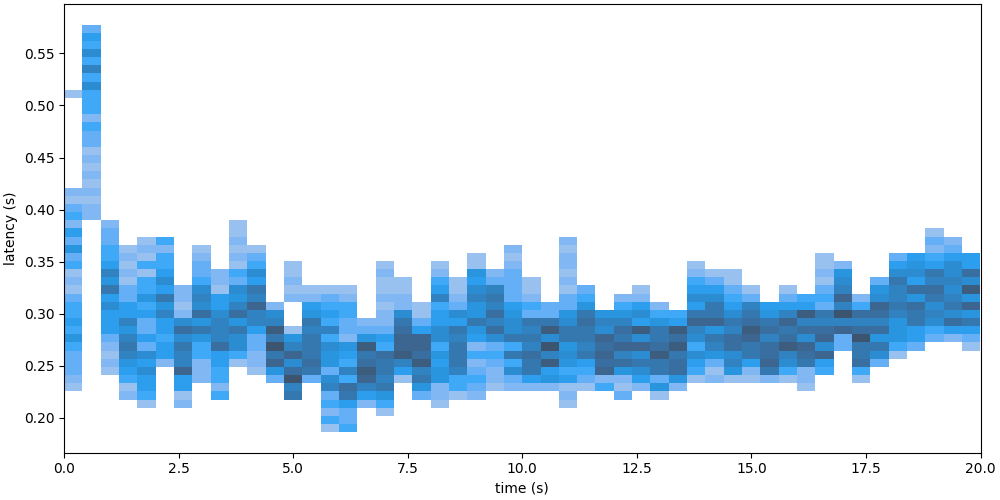
\includegraphics[scale=0.6]{heatmaps/batch_sizes_5_320_200_4_450_timelatencyheatmap.png}
\caption{Heatmap showing relatively stable latency throughout the course of the experiment. [add parameters!!]}
\label{stableheatmap}
\end{figure}

\begin{figure}[h!]
\centering
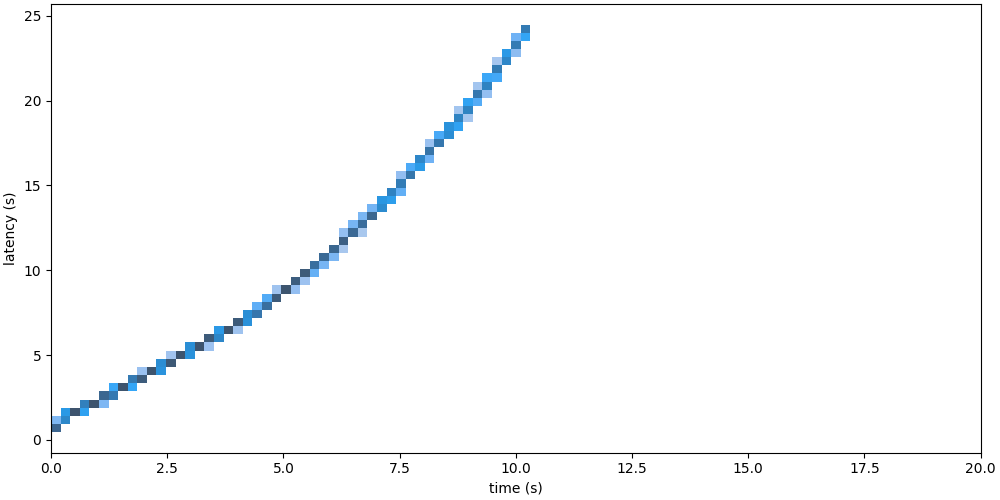
\includegraphics[scale=0.6]{heatmaps/batch_sizes_5_3_800_4_50_timelatencyheatmap.png}
\caption{Heatmap showing linear growth in latency as the experiment progresses. [add parameters]}
\label{linearheatmap}
\end{figure}

We now analyse the performance and behaviour of the system with different parameters, and under different conditions. We argue that the optimisations described in Section \ref{performance} were effective in improving system performance, but there are fundamental limitations caused by the latency costs of Cap'n Proto serialisation (Section \ref{capnpbenchmark}) and cryptography (Section \ref{tezosbenchmark}).

In most cases, the system exhibits stable latency throughout an experiment while goodput is equal to throughput, meaning that the system is not overloaded (Figure \ref{stableheatmap}). When the throughput exceeds the amount the system can keep up with, there is linear growth in latency as commands queue on the nodes (Figure \ref{linearheatmap}). Since HotStuff is a partially synchronous protocol (Section \ref{hotstufftheory}), an increase in latency means that view times increase, decreasing goodput. Once the system is overloaded, the goodput levels off at around its maximum value as throughput is increased.

In our comparison of batch sizes (Section \ref{batchsizeseval}) there is evidence that the implementation of batching (Section \ref{batching}) was effective, as the system is able to achieve much greater goodput with batch sizes greater than 1 (equivalent to no batching). This section also provides evidence that serialisation latency is a bottleneck, as view times begin to increase exponentially as batch sizes increase, due to messages being larger and taking longer to serialise.

Our study of node counts (Section \ref{nodecountseval}) gives further evidence that message serialisation is a bottleneck; higher node counts mean more internal messages being sent, causing a decline in performance due to serialisation costs. This also supports the conclusion that cryptography is a bottleneck, as more nodes means more messages must be signed and aggregated.

In our ablation study (Section \ref{ablation}) we compare the performance of the system with different optimisations enabled, demonstrating their effectiveness in increasing goodput, and lowering latency. We also demonstrate that cryptography is a bottleneck by demonstrating the superior performance of the system with cryptography disabled.

In our wide area network (WAN) simulation study (Section \ref{minineteval}), we compare the performance of our system running locally, to a simulated mininet network (Section \ref{testing}) with link latency similar to what one may observe in a wide area network. [we found...]

In our view-change study (Section \ref{viewchange}) we demonstrate that the view-change protocol (Section \ref{viewchange}) is effective in ensuring the system progresses once a node has died, albeit with a significant performance penalty.

\subsection{Batch sizes} \label{batchsizeseval}

\begin{figure}[h!]
\centering
%% Creator: Matplotlib, PGF backend
%%
%% To include the figure in your LaTeX document, write
%%   \input{<filename>.pgf}
%%
%% Make sure the required packages are loaded in your preamble
%%   \usepackage{pgf}
%%
%% Also ensure that all the required font packages are loaded; for instance,
%% the lmodern package is sometimes necessary when using math font.
%%   \usepackage{lmodern}
%%
%% Figures using additional raster images can only be included by \input if
%% they are in the same directory as the main LaTeX file. For loading figures
%% from other directories you can use the `import` package
%%   \usepackage{import}
%%
%% and then include the figures with
%%   \import{<path to file>}{<filename>.pgf}
%%
%% Matplotlib used the following preamble
%%   
%%   \usepackage{fontspec}
%%   \setmainfont{DejaVuSerif.ttf}[Path=\detokenize{/opt/homebrew/lib/python3.10/site-packages/matplotlib/mpl-data/fonts/ttf/}]
%%   \setsansfont{DejaVuSans.ttf}[Path=\detokenize{/opt/homebrew/lib/python3.10/site-packages/matplotlib/mpl-data/fonts/ttf/}]
%%   \setmonofont{DejaVuSansMono.ttf}[Path=\detokenize{/opt/homebrew/lib/python3.10/site-packages/matplotlib/mpl-data/fonts/ttf/}]
%%   \makeatletter\@ifpackageloaded{underscore}{}{\usepackage[strings]{underscore}}\makeatother
%%
\begingroup%
\makeatletter%
\begin{pgfpicture}%
\pgfpathrectangle{\pgfpointorigin}{\pgfqpoint{6.400000in}{4.800000in}}%
\pgfusepath{use as bounding box, clip}%
\begin{pgfscope}%
\pgfsetbuttcap%
\pgfsetmiterjoin%
\definecolor{currentfill}{rgb}{1.000000,1.000000,1.000000}%
\pgfsetfillcolor{currentfill}%
\pgfsetlinewidth{0.000000pt}%
\definecolor{currentstroke}{rgb}{1.000000,1.000000,1.000000}%
\pgfsetstrokecolor{currentstroke}%
\pgfsetdash{}{0pt}%
\pgfpathmoveto{\pgfqpoint{0.000000in}{0.000000in}}%
\pgfpathlineto{\pgfqpoint{6.400000in}{0.000000in}}%
\pgfpathlineto{\pgfqpoint{6.400000in}{4.800000in}}%
\pgfpathlineto{\pgfqpoint{0.000000in}{4.800000in}}%
\pgfpathlineto{\pgfqpoint{0.000000in}{0.000000in}}%
\pgfpathclose%
\pgfusepath{fill}%
\end{pgfscope}%
\begin{pgfscope}%
\pgfsetbuttcap%
\pgfsetmiterjoin%
\definecolor{currentfill}{rgb}{1.000000,1.000000,1.000000}%
\pgfsetfillcolor{currentfill}%
\pgfsetlinewidth{0.000000pt}%
\definecolor{currentstroke}{rgb}{0.000000,0.000000,0.000000}%
\pgfsetstrokecolor{currentstroke}%
\pgfsetstrokeopacity{0.000000}%
\pgfsetdash{}{0pt}%
\pgfpathmoveto{\pgfqpoint{0.800000in}{0.528000in}}%
\pgfpathlineto{\pgfqpoint{5.760000in}{0.528000in}}%
\pgfpathlineto{\pgfqpoint{5.760000in}{4.224000in}}%
\pgfpathlineto{\pgfqpoint{0.800000in}{4.224000in}}%
\pgfpathlineto{\pgfqpoint{0.800000in}{0.528000in}}%
\pgfpathclose%
\pgfusepath{fill}%
\end{pgfscope}%
\begin{pgfscope}%
\pgfpathrectangle{\pgfqpoint{0.800000in}{0.528000in}}{\pgfqpoint{4.960000in}{3.696000in}}%
\pgfusepath{clip}%
\pgfsetbuttcap%
\pgfsetroundjoin%
\definecolor{currentfill}{rgb}{0.003922,0.450980,0.698039}%
\pgfsetfillcolor{currentfill}%
\pgfsetfillopacity{0.200000}%
\pgfsetlinewidth{1.003750pt}%
\definecolor{currentstroke}{rgb}{0.003922,0.450980,0.698039}%
\pgfsetstrokecolor{currentstroke}%
\pgfsetstrokeopacity{0.200000}%
\pgfsetdash{}{0pt}%
\pgfpathmoveto{\pgfqpoint{0.802480in}{0.531696in}}%
\pgfpathlineto{\pgfqpoint{0.802480in}{0.531696in}}%
\pgfpathlineto{\pgfqpoint{0.862000in}{0.620383in}}%
\pgfpathlineto{\pgfqpoint{0.924000in}{0.712800in}}%
\pgfpathlineto{\pgfqpoint{1.048000in}{0.897304in}}%
\pgfpathlineto{\pgfqpoint{1.296000in}{1.265931in}}%
\pgfpathlineto{\pgfqpoint{1.792000in}{1.953887in}}%
\pgfpathlineto{\pgfqpoint{2.288000in}{2.263846in}}%
\pgfpathlineto{\pgfqpoint{2.784000in}{2.404237in}}%
\pgfpathlineto{\pgfqpoint{3.280000in}{2.570015in}}%
\pgfpathlineto{\pgfqpoint{3.776000in}{2.634051in}}%
\pgfpathlineto{\pgfqpoint{4.272000in}{2.685133in}}%
\pgfpathlineto{\pgfqpoint{4.768000in}{2.798333in}}%
\pgfpathlineto{\pgfqpoint{5.264000in}{2.827639in}}%
\pgfpathlineto{\pgfqpoint{5.760000in}{2.880518in}}%
\pgfpathlineto{\pgfqpoint{6.256000in}{2.754683in}}%
\pgfpathlineto{\pgfqpoint{6.752000in}{2.892815in}}%
\pgfpathlineto{\pgfqpoint{7.248000in}{2.866140in}}%
\pgfpathlineto{\pgfqpoint{7.744000in}{2.903008in}}%
\pgfpathlineto{\pgfqpoint{8.240000in}{2.858901in}}%
\pgfpathlineto{\pgfqpoint{8.736000in}{2.877058in}}%
\pgfpathlineto{\pgfqpoint{9.232000in}{2.940106in}}%
\pgfpathlineto{\pgfqpoint{9.728000in}{2.838385in}}%
\pgfpathlineto{\pgfqpoint{10.224000in}{2.879732in}}%
\pgfpathlineto{\pgfqpoint{10.720000in}{2.884800in}}%
\pgfpathlineto{\pgfqpoint{10.720000in}{7.261723in}}%
\pgfpathlineto{\pgfqpoint{10.720000in}{7.261723in}}%
\pgfpathlineto{\pgfqpoint{10.224000in}{7.175690in}}%
\pgfpathlineto{\pgfqpoint{9.728000in}{6.853113in}}%
\pgfpathlineto{\pgfqpoint{9.232000in}{6.726760in}}%
\pgfpathlineto{\pgfqpoint{8.736000in}{6.332100in}}%
\pgfpathlineto{\pgfqpoint{8.240000in}{6.135435in}}%
\pgfpathlineto{\pgfqpoint{7.744000in}{5.949950in}}%
\pgfpathlineto{\pgfqpoint{7.248000in}{5.856517in}}%
\pgfpathlineto{\pgfqpoint{6.752000in}{5.480693in}}%
\pgfpathlineto{\pgfqpoint{6.256000in}{5.374108in}}%
\pgfpathlineto{\pgfqpoint{5.760000in}{5.235068in}}%
\pgfpathlineto{\pgfqpoint{5.264000in}{4.975342in}}%
\pgfpathlineto{\pgfqpoint{4.768000in}{4.603880in}}%
\pgfpathlineto{\pgfqpoint{4.272000in}{4.314526in}}%
\pgfpathlineto{\pgfqpoint{3.776000in}{3.948612in}}%
\pgfpathlineto{\pgfqpoint{3.280000in}{3.554929in}}%
\pgfpathlineto{\pgfqpoint{2.784000in}{3.107268in}}%
\pgfpathlineto{\pgfqpoint{2.288000in}{2.614297in}}%
\pgfpathlineto{\pgfqpoint{1.792000in}{1.995632in}}%
\pgfpathlineto{\pgfqpoint{1.296000in}{1.267039in}}%
\pgfpathlineto{\pgfqpoint{1.048000in}{0.897592in}}%
\pgfpathlineto{\pgfqpoint{0.924000in}{0.712800in}}%
\pgfpathlineto{\pgfqpoint{0.862000in}{0.620400in}}%
\pgfpathlineto{\pgfqpoint{0.802480in}{0.531696in}}%
\pgfpathlineto{\pgfqpoint{0.802480in}{0.531696in}}%
\pgfpathclose%
\pgfusepath{stroke,fill}%
\end{pgfscope}%
\begin{pgfscope}%
\pgfsetbuttcap%
\pgfsetroundjoin%
\definecolor{currentfill}{rgb}{0.000000,0.000000,0.000000}%
\pgfsetfillcolor{currentfill}%
\pgfsetlinewidth{0.803000pt}%
\definecolor{currentstroke}{rgb}{0.000000,0.000000,0.000000}%
\pgfsetstrokecolor{currentstroke}%
\pgfsetdash{}{0pt}%
\pgfsys@defobject{currentmarker}{\pgfqpoint{0.000000in}{-0.048611in}}{\pgfqpoint{0.000000in}{0.000000in}}{%
\pgfpathmoveto{\pgfqpoint{0.000000in}{0.000000in}}%
\pgfpathlineto{\pgfqpoint{0.000000in}{-0.048611in}}%
\pgfusepath{stroke,fill}%
}%
\begin{pgfscope}%
\pgfsys@transformshift{0.800000in}{0.528000in}%
\pgfsys@useobject{currentmarker}{}%
\end{pgfscope}%
\end{pgfscope}%
\begin{pgfscope}%
\definecolor{textcolor}{rgb}{0.000000,0.000000,0.000000}%
\pgfsetstrokecolor{textcolor}%
\pgfsetfillcolor{textcolor}%
\pgftext[x=0.800000in,y=0.430778in,,top]{\color{textcolor}\sffamily\fontsize{10.000000}{12.000000}\selectfont 0}%
\end{pgfscope}%
\begin{pgfscope}%
\pgfsetbuttcap%
\pgfsetroundjoin%
\definecolor{currentfill}{rgb}{0.000000,0.000000,0.000000}%
\pgfsetfillcolor{currentfill}%
\pgfsetlinewidth{0.803000pt}%
\definecolor{currentstroke}{rgb}{0.000000,0.000000,0.000000}%
\pgfsetstrokecolor{currentstroke}%
\pgfsetdash{}{0pt}%
\pgfsys@defobject{currentmarker}{\pgfqpoint{0.000000in}{-0.048611in}}{\pgfqpoint{0.000000in}{0.000000in}}{%
\pgfpathmoveto{\pgfqpoint{0.000000in}{0.000000in}}%
\pgfpathlineto{\pgfqpoint{0.000000in}{-0.048611in}}%
\pgfusepath{stroke,fill}%
}%
\begin{pgfscope}%
\pgfsys@transformshift{1.420000in}{0.528000in}%
\pgfsys@useobject{currentmarker}{}%
\end{pgfscope}%
\end{pgfscope}%
\begin{pgfscope}%
\definecolor{textcolor}{rgb}{0.000000,0.000000,0.000000}%
\pgfsetstrokecolor{textcolor}%
\pgfsetfillcolor{textcolor}%
\pgftext[x=1.420000in,y=0.430778in,,top]{\color{textcolor}\sffamily\fontsize{10.000000}{12.000000}\selectfont 250}%
\end{pgfscope}%
\begin{pgfscope}%
\pgfsetbuttcap%
\pgfsetroundjoin%
\definecolor{currentfill}{rgb}{0.000000,0.000000,0.000000}%
\pgfsetfillcolor{currentfill}%
\pgfsetlinewidth{0.803000pt}%
\definecolor{currentstroke}{rgb}{0.000000,0.000000,0.000000}%
\pgfsetstrokecolor{currentstroke}%
\pgfsetdash{}{0pt}%
\pgfsys@defobject{currentmarker}{\pgfqpoint{0.000000in}{-0.048611in}}{\pgfqpoint{0.000000in}{0.000000in}}{%
\pgfpathmoveto{\pgfqpoint{0.000000in}{0.000000in}}%
\pgfpathlineto{\pgfqpoint{0.000000in}{-0.048611in}}%
\pgfusepath{stroke,fill}%
}%
\begin{pgfscope}%
\pgfsys@transformshift{2.040000in}{0.528000in}%
\pgfsys@useobject{currentmarker}{}%
\end{pgfscope}%
\end{pgfscope}%
\begin{pgfscope}%
\definecolor{textcolor}{rgb}{0.000000,0.000000,0.000000}%
\pgfsetstrokecolor{textcolor}%
\pgfsetfillcolor{textcolor}%
\pgftext[x=2.040000in,y=0.430778in,,top]{\color{textcolor}\sffamily\fontsize{10.000000}{12.000000}\selectfont 500}%
\end{pgfscope}%
\begin{pgfscope}%
\pgfsetbuttcap%
\pgfsetroundjoin%
\definecolor{currentfill}{rgb}{0.000000,0.000000,0.000000}%
\pgfsetfillcolor{currentfill}%
\pgfsetlinewidth{0.803000pt}%
\definecolor{currentstroke}{rgb}{0.000000,0.000000,0.000000}%
\pgfsetstrokecolor{currentstroke}%
\pgfsetdash{}{0pt}%
\pgfsys@defobject{currentmarker}{\pgfqpoint{0.000000in}{-0.048611in}}{\pgfqpoint{0.000000in}{0.000000in}}{%
\pgfpathmoveto{\pgfqpoint{0.000000in}{0.000000in}}%
\pgfpathlineto{\pgfqpoint{0.000000in}{-0.048611in}}%
\pgfusepath{stroke,fill}%
}%
\begin{pgfscope}%
\pgfsys@transformshift{2.660000in}{0.528000in}%
\pgfsys@useobject{currentmarker}{}%
\end{pgfscope}%
\end{pgfscope}%
\begin{pgfscope}%
\definecolor{textcolor}{rgb}{0.000000,0.000000,0.000000}%
\pgfsetstrokecolor{textcolor}%
\pgfsetfillcolor{textcolor}%
\pgftext[x=2.660000in,y=0.430778in,,top]{\color{textcolor}\sffamily\fontsize{10.000000}{12.000000}\selectfont 750}%
\end{pgfscope}%
\begin{pgfscope}%
\pgfsetbuttcap%
\pgfsetroundjoin%
\definecolor{currentfill}{rgb}{0.000000,0.000000,0.000000}%
\pgfsetfillcolor{currentfill}%
\pgfsetlinewidth{0.803000pt}%
\definecolor{currentstroke}{rgb}{0.000000,0.000000,0.000000}%
\pgfsetstrokecolor{currentstroke}%
\pgfsetdash{}{0pt}%
\pgfsys@defobject{currentmarker}{\pgfqpoint{0.000000in}{-0.048611in}}{\pgfqpoint{0.000000in}{0.000000in}}{%
\pgfpathmoveto{\pgfqpoint{0.000000in}{0.000000in}}%
\pgfpathlineto{\pgfqpoint{0.000000in}{-0.048611in}}%
\pgfusepath{stroke,fill}%
}%
\begin{pgfscope}%
\pgfsys@transformshift{3.280000in}{0.528000in}%
\pgfsys@useobject{currentmarker}{}%
\end{pgfscope}%
\end{pgfscope}%
\begin{pgfscope}%
\definecolor{textcolor}{rgb}{0.000000,0.000000,0.000000}%
\pgfsetstrokecolor{textcolor}%
\pgfsetfillcolor{textcolor}%
\pgftext[x=3.280000in,y=0.430778in,,top]{\color{textcolor}\sffamily\fontsize{10.000000}{12.000000}\selectfont 1000}%
\end{pgfscope}%
\begin{pgfscope}%
\pgfsetbuttcap%
\pgfsetroundjoin%
\definecolor{currentfill}{rgb}{0.000000,0.000000,0.000000}%
\pgfsetfillcolor{currentfill}%
\pgfsetlinewidth{0.803000pt}%
\definecolor{currentstroke}{rgb}{0.000000,0.000000,0.000000}%
\pgfsetstrokecolor{currentstroke}%
\pgfsetdash{}{0pt}%
\pgfsys@defobject{currentmarker}{\pgfqpoint{0.000000in}{-0.048611in}}{\pgfqpoint{0.000000in}{0.000000in}}{%
\pgfpathmoveto{\pgfqpoint{0.000000in}{0.000000in}}%
\pgfpathlineto{\pgfqpoint{0.000000in}{-0.048611in}}%
\pgfusepath{stroke,fill}%
}%
\begin{pgfscope}%
\pgfsys@transformshift{3.900000in}{0.528000in}%
\pgfsys@useobject{currentmarker}{}%
\end{pgfscope}%
\end{pgfscope}%
\begin{pgfscope}%
\definecolor{textcolor}{rgb}{0.000000,0.000000,0.000000}%
\pgfsetstrokecolor{textcolor}%
\pgfsetfillcolor{textcolor}%
\pgftext[x=3.900000in,y=0.430778in,,top]{\color{textcolor}\sffamily\fontsize{10.000000}{12.000000}\selectfont 1250}%
\end{pgfscope}%
\begin{pgfscope}%
\pgfsetbuttcap%
\pgfsetroundjoin%
\definecolor{currentfill}{rgb}{0.000000,0.000000,0.000000}%
\pgfsetfillcolor{currentfill}%
\pgfsetlinewidth{0.803000pt}%
\definecolor{currentstroke}{rgb}{0.000000,0.000000,0.000000}%
\pgfsetstrokecolor{currentstroke}%
\pgfsetdash{}{0pt}%
\pgfsys@defobject{currentmarker}{\pgfqpoint{0.000000in}{-0.048611in}}{\pgfqpoint{0.000000in}{0.000000in}}{%
\pgfpathmoveto{\pgfqpoint{0.000000in}{0.000000in}}%
\pgfpathlineto{\pgfqpoint{0.000000in}{-0.048611in}}%
\pgfusepath{stroke,fill}%
}%
\begin{pgfscope}%
\pgfsys@transformshift{4.520000in}{0.528000in}%
\pgfsys@useobject{currentmarker}{}%
\end{pgfscope}%
\end{pgfscope}%
\begin{pgfscope}%
\definecolor{textcolor}{rgb}{0.000000,0.000000,0.000000}%
\pgfsetstrokecolor{textcolor}%
\pgfsetfillcolor{textcolor}%
\pgftext[x=4.520000in,y=0.430778in,,top]{\color{textcolor}\sffamily\fontsize{10.000000}{12.000000}\selectfont 1500}%
\end{pgfscope}%
\begin{pgfscope}%
\pgfsetbuttcap%
\pgfsetroundjoin%
\definecolor{currentfill}{rgb}{0.000000,0.000000,0.000000}%
\pgfsetfillcolor{currentfill}%
\pgfsetlinewidth{0.803000pt}%
\definecolor{currentstroke}{rgb}{0.000000,0.000000,0.000000}%
\pgfsetstrokecolor{currentstroke}%
\pgfsetdash{}{0pt}%
\pgfsys@defobject{currentmarker}{\pgfqpoint{0.000000in}{-0.048611in}}{\pgfqpoint{0.000000in}{0.000000in}}{%
\pgfpathmoveto{\pgfqpoint{0.000000in}{0.000000in}}%
\pgfpathlineto{\pgfqpoint{0.000000in}{-0.048611in}}%
\pgfusepath{stroke,fill}%
}%
\begin{pgfscope}%
\pgfsys@transformshift{5.140000in}{0.528000in}%
\pgfsys@useobject{currentmarker}{}%
\end{pgfscope}%
\end{pgfscope}%
\begin{pgfscope}%
\definecolor{textcolor}{rgb}{0.000000,0.000000,0.000000}%
\pgfsetstrokecolor{textcolor}%
\pgfsetfillcolor{textcolor}%
\pgftext[x=5.140000in,y=0.430778in,,top]{\color{textcolor}\sffamily\fontsize{10.000000}{12.000000}\selectfont 1750}%
\end{pgfscope}%
\begin{pgfscope}%
\pgfsetbuttcap%
\pgfsetroundjoin%
\definecolor{currentfill}{rgb}{0.000000,0.000000,0.000000}%
\pgfsetfillcolor{currentfill}%
\pgfsetlinewidth{0.803000pt}%
\definecolor{currentstroke}{rgb}{0.000000,0.000000,0.000000}%
\pgfsetstrokecolor{currentstroke}%
\pgfsetdash{}{0pt}%
\pgfsys@defobject{currentmarker}{\pgfqpoint{0.000000in}{-0.048611in}}{\pgfqpoint{0.000000in}{0.000000in}}{%
\pgfpathmoveto{\pgfqpoint{0.000000in}{0.000000in}}%
\pgfpathlineto{\pgfqpoint{0.000000in}{-0.048611in}}%
\pgfusepath{stroke,fill}%
}%
\begin{pgfscope}%
\pgfsys@transformshift{5.760000in}{0.528000in}%
\pgfsys@useobject{currentmarker}{}%
\end{pgfscope}%
\end{pgfscope}%
\begin{pgfscope}%
\definecolor{textcolor}{rgb}{0.000000,0.000000,0.000000}%
\pgfsetstrokecolor{textcolor}%
\pgfsetfillcolor{textcolor}%
\pgftext[x=5.760000in,y=0.430778in,,top]{\color{textcolor}\sffamily\fontsize{10.000000}{12.000000}\selectfont 2000}%
\end{pgfscope}%
\begin{pgfscope}%
\definecolor{textcolor}{rgb}{0.000000,0.000000,0.000000}%
\pgfsetstrokecolor{textcolor}%
\pgfsetfillcolor{textcolor}%
\pgftext[x=3.280000in,y=0.240809in,,top]{\color{textcolor}\sffamily\fontsize{10.000000}{12.000000}\selectfont throughput (req/s)}%
\end{pgfscope}%
\begin{pgfscope}%
\pgfsetbuttcap%
\pgfsetroundjoin%
\definecolor{currentfill}{rgb}{0.000000,0.000000,0.000000}%
\pgfsetfillcolor{currentfill}%
\pgfsetlinewidth{0.803000pt}%
\definecolor{currentstroke}{rgb}{0.000000,0.000000,0.000000}%
\pgfsetstrokecolor{currentstroke}%
\pgfsetdash{}{0pt}%
\pgfsys@defobject{currentmarker}{\pgfqpoint{-0.048611in}{0.000000in}}{\pgfqpoint{-0.000000in}{0.000000in}}{%
\pgfpathmoveto{\pgfqpoint{-0.000000in}{0.000000in}}%
\pgfpathlineto{\pgfqpoint{-0.048611in}{0.000000in}}%
\pgfusepath{stroke,fill}%
}%
\begin{pgfscope}%
\pgfsys@transformshift{0.800000in}{0.528000in}%
\pgfsys@useobject{currentmarker}{}%
\end{pgfscope}%
\end{pgfscope}%
\begin{pgfscope}%
\definecolor{textcolor}{rgb}{0.000000,0.000000,0.000000}%
\pgfsetstrokecolor{textcolor}%
\pgfsetfillcolor{textcolor}%
\pgftext[x=0.614412in, y=0.475238in, left, base]{\color{textcolor}\sffamily\fontsize{10.000000}{12.000000}\selectfont 0}%
\end{pgfscope}%
\begin{pgfscope}%
\pgfsetbuttcap%
\pgfsetroundjoin%
\definecolor{currentfill}{rgb}{0.000000,0.000000,0.000000}%
\pgfsetfillcolor{currentfill}%
\pgfsetlinewidth{0.803000pt}%
\definecolor{currentstroke}{rgb}{0.000000,0.000000,0.000000}%
\pgfsetstrokecolor{currentstroke}%
\pgfsetdash{}{0pt}%
\pgfsys@defobject{currentmarker}{\pgfqpoint{-0.048611in}{0.000000in}}{\pgfqpoint{-0.000000in}{0.000000in}}{%
\pgfpathmoveto{\pgfqpoint{-0.000000in}{0.000000in}}%
\pgfpathlineto{\pgfqpoint{-0.048611in}{0.000000in}}%
\pgfusepath{stroke,fill}%
}%
\begin{pgfscope}%
\pgfsys@transformshift{0.800000in}{1.267200in}%
\pgfsys@useobject{currentmarker}{}%
\end{pgfscope}%
\end{pgfscope}%
\begin{pgfscope}%
\definecolor{textcolor}{rgb}{0.000000,0.000000,0.000000}%
\pgfsetstrokecolor{textcolor}%
\pgfsetfillcolor{textcolor}%
\pgftext[x=0.437682in, y=1.214438in, left, base]{\color{textcolor}\sffamily\fontsize{10.000000}{12.000000}\selectfont 200}%
\end{pgfscope}%
\begin{pgfscope}%
\pgfsetbuttcap%
\pgfsetroundjoin%
\definecolor{currentfill}{rgb}{0.000000,0.000000,0.000000}%
\pgfsetfillcolor{currentfill}%
\pgfsetlinewidth{0.803000pt}%
\definecolor{currentstroke}{rgb}{0.000000,0.000000,0.000000}%
\pgfsetstrokecolor{currentstroke}%
\pgfsetdash{}{0pt}%
\pgfsys@defobject{currentmarker}{\pgfqpoint{-0.048611in}{0.000000in}}{\pgfqpoint{-0.000000in}{0.000000in}}{%
\pgfpathmoveto{\pgfqpoint{-0.000000in}{0.000000in}}%
\pgfpathlineto{\pgfqpoint{-0.048611in}{0.000000in}}%
\pgfusepath{stroke,fill}%
}%
\begin{pgfscope}%
\pgfsys@transformshift{0.800000in}{2.006400in}%
\pgfsys@useobject{currentmarker}{}%
\end{pgfscope}%
\end{pgfscope}%
\begin{pgfscope}%
\definecolor{textcolor}{rgb}{0.000000,0.000000,0.000000}%
\pgfsetstrokecolor{textcolor}%
\pgfsetfillcolor{textcolor}%
\pgftext[x=0.437682in, y=1.953638in, left, base]{\color{textcolor}\sffamily\fontsize{10.000000}{12.000000}\selectfont 400}%
\end{pgfscope}%
\begin{pgfscope}%
\pgfsetbuttcap%
\pgfsetroundjoin%
\definecolor{currentfill}{rgb}{0.000000,0.000000,0.000000}%
\pgfsetfillcolor{currentfill}%
\pgfsetlinewidth{0.803000pt}%
\definecolor{currentstroke}{rgb}{0.000000,0.000000,0.000000}%
\pgfsetstrokecolor{currentstroke}%
\pgfsetdash{}{0pt}%
\pgfsys@defobject{currentmarker}{\pgfqpoint{-0.048611in}{0.000000in}}{\pgfqpoint{-0.000000in}{0.000000in}}{%
\pgfpathmoveto{\pgfqpoint{-0.000000in}{0.000000in}}%
\pgfpathlineto{\pgfqpoint{-0.048611in}{0.000000in}}%
\pgfusepath{stroke,fill}%
}%
\begin{pgfscope}%
\pgfsys@transformshift{0.800000in}{2.745600in}%
\pgfsys@useobject{currentmarker}{}%
\end{pgfscope}%
\end{pgfscope}%
\begin{pgfscope}%
\definecolor{textcolor}{rgb}{0.000000,0.000000,0.000000}%
\pgfsetstrokecolor{textcolor}%
\pgfsetfillcolor{textcolor}%
\pgftext[x=0.437682in, y=2.692838in, left, base]{\color{textcolor}\sffamily\fontsize{10.000000}{12.000000}\selectfont 600}%
\end{pgfscope}%
\begin{pgfscope}%
\pgfsetbuttcap%
\pgfsetroundjoin%
\definecolor{currentfill}{rgb}{0.000000,0.000000,0.000000}%
\pgfsetfillcolor{currentfill}%
\pgfsetlinewidth{0.803000pt}%
\definecolor{currentstroke}{rgb}{0.000000,0.000000,0.000000}%
\pgfsetstrokecolor{currentstroke}%
\pgfsetdash{}{0pt}%
\pgfsys@defobject{currentmarker}{\pgfqpoint{-0.048611in}{0.000000in}}{\pgfqpoint{-0.000000in}{0.000000in}}{%
\pgfpathmoveto{\pgfqpoint{-0.000000in}{0.000000in}}%
\pgfpathlineto{\pgfqpoint{-0.048611in}{0.000000in}}%
\pgfusepath{stroke,fill}%
}%
\begin{pgfscope}%
\pgfsys@transformshift{0.800000in}{3.484800in}%
\pgfsys@useobject{currentmarker}{}%
\end{pgfscope}%
\end{pgfscope}%
\begin{pgfscope}%
\definecolor{textcolor}{rgb}{0.000000,0.000000,0.000000}%
\pgfsetstrokecolor{textcolor}%
\pgfsetfillcolor{textcolor}%
\pgftext[x=0.437682in, y=3.432038in, left, base]{\color{textcolor}\sffamily\fontsize{10.000000}{12.000000}\selectfont 800}%
\end{pgfscope}%
\begin{pgfscope}%
\pgfsetbuttcap%
\pgfsetroundjoin%
\definecolor{currentfill}{rgb}{0.000000,0.000000,0.000000}%
\pgfsetfillcolor{currentfill}%
\pgfsetlinewidth{0.803000pt}%
\definecolor{currentstroke}{rgb}{0.000000,0.000000,0.000000}%
\pgfsetstrokecolor{currentstroke}%
\pgfsetdash{}{0pt}%
\pgfsys@defobject{currentmarker}{\pgfqpoint{-0.048611in}{0.000000in}}{\pgfqpoint{-0.000000in}{0.000000in}}{%
\pgfpathmoveto{\pgfqpoint{-0.000000in}{0.000000in}}%
\pgfpathlineto{\pgfqpoint{-0.048611in}{0.000000in}}%
\pgfusepath{stroke,fill}%
}%
\begin{pgfscope}%
\pgfsys@transformshift{0.800000in}{4.224000in}%
\pgfsys@useobject{currentmarker}{}%
\end{pgfscope}%
\end{pgfscope}%
\begin{pgfscope}%
\definecolor{textcolor}{rgb}{0.000000,0.000000,0.000000}%
\pgfsetstrokecolor{textcolor}%
\pgfsetfillcolor{textcolor}%
\pgftext[x=0.349316in, y=4.171238in, left, base]{\color{textcolor}\sffamily\fontsize{10.000000}{12.000000}\selectfont 1000}%
\end{pgfscope}%
\begin{pgfscope}%
\definecolor{textcolor}{rgb}{0.000000,0.000000,0.000000}%
\pgfsetstrokecolor{textcolor}%
\pgfsetfillcolor{textcolor}%
\pgftext[x=0.293761in,y=2.376000in,,bottom,rotate=90.000000]{\color{textcolor}\sffamily\fontsize{10.000000}{12.000000}\selectfont goodput (req/s)}%
\end{pgfscope}%
\begin{pgfscope}%
\pgfpathrectangle{\pgfqpoint{0.800000in}{0.528000in}}{\pgfqpoint{4.960000in}{3.696000in}}%
\pgfusepath{clip}%
\pgfsetbuttcap%
\pgfsetroundjoin%
\pgfsetlinewidth{1.505625pt}%
\definecolor{currentstroke}{rgb}{0.003922,0.450980,0.698039}%
\pgfsetstrokecolor{currentstroke}%
\pgfsetdash{{5.550000pt}{2.400000pt}}{0.000000pt}%
\pgfpathmoveto{\pgfqpoint{0.802480in}{0.531696in}}%
\pgfpathlineto{\pgfqpoint{0.862000in}{0.620394in}}%
\pgfpathlineto{\pgfqpoint{0.924000in}{0.712800in}}%
\pgfpathlineto{\pgfqpoint{1.048000in}{0.897482in}}%
\pgfpathlineto{\pgfqpoint{1.296000in}{1.266553in}}%
\pgfpathlineto{\pgfqpoint{1.792000in}{1.977061in}}%
\pgfpathlineto{\pgfqpoint{2.288000in}{2.444062in}}%
\pgfpathlineto{\pgfqpoint{2.784000in}{2.764210in}}%
\pgfpathlineto{\pgfqpoint{3.280000in}{3.041182in}}%
\pgfpathlineto{\pgfqpoint{3.776000in}{3.292672in}}%
\pgfpathlineto{\pgfqpoint{4.272000in}{3.469831in}}%
\pgfpathlineto{\pgfqpoint{4.768000in}{3.678780in}}%
\pgfpathlineto{\pgfqpoint{5.264000in}{3.853168in}}%
\pgfpathlineto{\pgfqpoint{5.760000in}{4.010204in}}%
\pgfpathlineto{\pgfqpoint{5.770000in}{4.011028in}}%
\pgfusepath{stroke}%
\end{pgfscope}%
\begin{pgfscope}%
\pgfsetrectcap%
\pgfsetmiterjoin%
\pgfsetlinewidth{0.803000pt}%
\definecolor{currentstroke}{rgb}{0.000000,0.000000,0.000000}%
\pgfsetstrokecolor{currentstroke}%
\pgfsetdash{}{0pt}%
\pgfpathmoveto{\pgfqpoint{0.800000in}{0.528000in}}%
\pgfpathlineto{\pgfqpoint{0.800000in}{4.224000in}}%
\pgfusepath{stroke}%
\end{pgfscope}%
\begin{pgfscope}%
\pgfsetrectcap%
\pgfsetmiterjoin%
\pgfsetlinewidth{0.803000pt}%
\definecolor{currentstroke}{rgb}{0.000000,0.000000,0.000000}%
\pgfsetstrokecolor{currentstroke}%
\pgfsetdash{}{0pt}%
\pgfpathmoveto{\pgfqpoint{5.760000in}{0.528000in}}%
\pgfpathlineto{\pgfqpoint{5.760000in}{4.224000in}}%
\pgfusepath{stroke}%
\end{pgfscope}%
\begin{pgfscope}%
\pgfsetrectcap%
\pgfsetmiterjoin%
\pgfsetlinewidth{0.803000pt}%
\definecolor{currentstroke}{rgb}{0.000000,0.000000,0.000000}%
\pgfsetstrokecolor{currentstroke}%
\pgfsetdash{}{0pt}%
\pgfpathmoveto{\pgfqpoint{0.800000in}{0.528000in}}%
\pgfpathlineto{\pgfqpoint{5.760000in}{0.528000in}}%
\pgfusepath{stroke}%
\end{pgfscope}%
\begin{pgfscope}%
\pgfsetrectcap%
\pgfsetmiterjoin%
\pgfsetlinewidth{0.803000pt}%
\definecolor{currentstroke}{rgb}{0.000000,0.000000,0.000000}%
\pgfsetstrokecolor{currentstroke}%
\pgfsetdash{}{0pt}%
\pgfpathmoveto{\pgfqpoint{0.800000in}{4.224000in}}%
\pgfpathlineto{\pgfqpoint{5.760000in}{4.224000in}}%
\pgfusepath{stroke}%
\end{pgfscope}%
\begin{pgfscope}%
\pgfsetbuttcap%
\pgfsetmiterjoin%
\definecolor{currentfill}{rgb}{1.000000,1.000000,1.000000}%
\pgfsetfillcolor{currentfill}%
\pgfsetfillopacity{0.800000}%
\pgfsetlinewidth{1.003750pt}%
\definecolor{currentstroke}{rgb}{0.800000,0.800000,0.800000}%
\pgfsetstrokecolor{currentstroke}%
\pgfsetstrokeopacity{0.800000}%
\pgfsetdash{}{0pt}%
\pgfpathmoveto{\pgfqpoint{0.897222in}{3.705174in}}%
\pgfpathlineto{\pgfqpoint{1.658344in}{3.705174in}}%
\pgfpathquadraticcurveto{\pgfqpoint{1.686122in}{3.705174in}}{\pgfqpoint{1.686122in}{3.732952in}}%
\pgfpathlineto{\pgfqpoint{1.686122in}{4.126778in}}%
\pgfpathquadraticcurveto{\pgfqpoint{1.686122in}{4.154556in}}{\pgfqpoint{1.658344in}{4.154556in}}%
\pgfpathlineto{\pgfqpoint{0.897222in}{4.154556in}}%
\pgfpathquadraticcurveto{\pgfqpoint{0.869444in}{4.154556in}}{\pgfqpoint{0.869444in}{4.126778in}}%
\pgfpathlineto{\pgfqpoint{0.869444in}{3.732952in}}%
\pgfpathquadraticcurveto{\pgfqpoint{0.869444in}{3.705174in}}{\pgfqpoint{0.897222in}{3.705174in}}%
\pgfpathlineto{\pgfqpoint{0.897222in}{3.705174in}}%
\pgfpathclose%
\pgfusepath{stroke,fill}%
\end{pgfscope}%
\begin{pgfscope}%
\definecolor{textcolor}{rgb}{0.000000,0.000000,0.000000}%
\pgfsetstrokecolor{textcolor}%
\pgfsetfillcolor{textcolor}%
\pgftext[x=0.925000in,y=3.993477in,left,base]{\color{textcolor}\sffamily\fontsize{10.000000}{12.000000}\selectfont batch size}%
\end{pgfscope}%
\begin{pgfscope}%
\pgfsetrectcap%
\pgfsetroundjoin%
\pgfsetlinewidth{1.505625pt}%
\definecolor{currentstroke}{rgb}{0.003922,0.450980,0.698039}%
\pgfsetstrokecolor{currentstroke}%
\pgfsetdash{}{0pt}%
\pgfpathmoveto{\pgfqpoint{0.950791in}{3.838231in}}%
\pgfpathlineto{\pgfqpoint{1.089680in}{3.838231in}}%
\pgfpathlineto{\pgfqpoint{1.228569in}{3.838231in}}%
\pgfusepath{stroke}%
\end{pgfscope}%
\begin{pgfscope}%
\definecolor{textcolor}{rgb}{0.000000,0.000000,0.000000}%
\pgfsetstrokecolor{textcolor}%
\pgfsetfillcolor{textcolor}%
\pgftext[x=1.339680in,y=3.789620in,left,base]{\color{textcolor}\sffamily\fontsize{10.000000}{12.000000}\selectfont 300}%
\end{pgfscope}%
\end{pgfpicture}%
\makeatother%
\endgroup%

\caption{Benchmarking of goodput for varying throughputs and batch sizes.}
\label{throughputgoodputbatch}
\end{figure}

\begin{figure}[h!]
\centering
%% Creator: Matplotlib, PGF backend
%%
%% To include the figure in your LaTeX document, write
%%   \input{<filename>.pgf}
%%
%% Make sure the required packages are loaded in your preamble
%%   \usepackage{pgf}
%%
%% Also ensure that all the required font packages are loaded; for instance,
%% the lmodern package is sometimes necessary when using math font.
%%   \usepackage{lmodern}
%%
%% Figures using additional raster images can only be included by \input if
%% they are in the same directory as the main LaTeX file. For loading figures
%% from other directories you can use the `import` package
%%   \usepackage{import}
%%
%% and then include the figures with
%%   \import{<path to file>}{<filename>.pgf}
%%
%% Matplotlib used the following preamble
%%   
%%   \usepackage{fontspec}
%%   \setmainfont{DejaVuSerif.ttf}[Path=\detokenize{/opt/homebrew/lib/python3.10/site-packages/matplotlib/mpl-data/fonts/ttf/}]
%%   \setsansfont{DejaVuSans.ttf}[Path=\detokenize{/opt/homebrew/lib/python3.10/site-packages/matplotlib/mpl-data/fonts/ttf/}]
%%   \setmonofont{DejaVuSansMono.ttf}[Path=\detokenize{/opt/homebrew/lib/python3.10/site-packages/matplotlib/mpl-data/fonts/ttf/}]
%%   \makeatletter\@ifpackageloaded{underscore}{}{\usepackage[strings]{underscore}}\makeatother
%%
\begingroup%
\makeatletter%
\begin{pgfpicture}%
\pgfpathrectangle{\pgfpointorigin}{\pgfqpoint{5.840000in}{5.000000in}}%
\pgfusepath{use as bounding box, clip}%
\begin{pgfscope}%
\pgfsetbuttcap%
\pgfsetmiterjoin%
\definecolor{currentfill}{rgb}{1.000000,1.000000,1.000000}%
\pgfsetfillcolor{currentfill}%
\pgfsetlinewidth{0.000000pt}%
\definecolor{currentstroke}{rgb}{1.000000,1.000000,1.000000}%
\pgfsetstrokecolor{currentstroke}%
\pgfsetdash{}{0pt}%
\pgfpathmoveto{\pgfqpoint{0.000000in}{0.000000in}}%
\pgfpathlineto{\pgfqpoint{5.840000in}{0.000000in}}%
\pgfpathlineto{\pgfqpoint{5.840000in}{5.000000in}}%
\pgfpathlineto{\pgfqpoint{0.000000in}{5.000000in}}%
\pgfpathlineto{\pgfqpoint{0.000000in}{0.000000in}}%
\pgfpathclose%
\pgfusepath{fill}%
\end{pgfscope}%
\begin{pgfscope}%
\pgfsetbuttcap%
\pgfsetmiterjoin%
\definecolor{currentfill}{rgb}{1.000000,1.000000,1.000000}%
\pgfsetfillcolor{currentfill}%
\pgfsetlinewidth{0.000000pt}%
\definecolor{currentstroke}{rgb}{0.000000,0.000000,0.000000}%
\pgfsetstrokecolor{currentstroke}%
\pgfsetstrokeopacity{0.000000}%
\pgfsetdash{}{0pt}%
\pgfpathmoveto{\pgfqpoint{0.775584in}{0.582778in}}%
\pgfpathlineto{\pgfqpoint{4.939579in}{0.582778in}}%
\pgfpathlineto{\pgfqpoint{4.939579in}{4.850000in}}%
\pgfpathlineto{\pgfqpoint{0.775584in}{4.850000in}}%
\pgfpathlineto{\pgfqpoint{0.775584in}{0.582778in}}%
\pgfpathclose%
\pgfusepath{fill}%
\end{pgfscope}%
\begin{pgfscope}%
\pgfpathrectangle{\pgfqpoint{0.775584in}{0.582778in}}{\pgfqpoint{4.163995in}{4.267222in}}%
\pgfusepath{clip}%
\pgfsetbuttcap%
\pgfsetroundjoin%
\definecolor{currentfill}{rgb}{0.003922,0.450980,0.698039}%
\pgfsetfillcolor{currentfill}%
\pgfsetfillopacity{0.800000}%
\pgfsetlinewidth{1.003750pt}%
\definecolor{currentstroke}{rgb}{0.003922,0.450980,0.698039}%
\pgfsetstrokecolor{currentstroke}%
\pgfsetstrokeopacity{0.800000}%
\pgfsetdash{}{0pt}%
\pgfsys@defobject{currentmarker}{\pgfqpoint{-0.041667in}{-0.041667in}}{\pgfqpoint{0.041667in}{0.041667in}}{%
\pgfpathmoveto{\pgfqpoint{0.000000in}{-0.041667in}}%
\pgfpathcurveto{\pgfqpoint{0.011050in}{-0.041667in}}{\pgfqpoint{0.021649in}{-0.037276in}}{\pgfqpoint{0.029463in}{-0.029463in}}%
\pgfpathcurveto{\pgfqpoint{0.037276in}{-0.021649in}}{\pgfqpoint{0.041667in}{-0.011050in}}{\pgfqpoint{0.041667in}{0.000000in}}%
\pgfpathcurveto{\pgfqpoint{0.041667in}{0.011050in}}{\pgfqpoint{0.037276in}{0.021649in}}{\pgfqpoint{0.029463in}{0.029463in}}%
\pgfpathcurveto{\pgfqpoint{0.021649in}{0.037276in}}{\pgfqpoint{0.011050in}{0.041667in}}{\pgfqpoint{0.000000in}{0.041667in}}%
\pgfpathcurveto{\pgfqpoint{-0.011050in}{0.041667in}}{\pgfqpoint{-0.021649in}{0.037276in}}{\pgfqpoint{-0.029463in}{0.029463in}}%
\pgfpathcurveto{\pgfqpoint{-0.037276in}{0.021649in}}{\pgfqpoint{-0.041667in}{0.011050in}}{\pgfqpoint{-0.041667in}{0.000000in}}%
\pgfpathcurveto{\pgfqpoint{-0.041667in}{-0.011050in}}{\pgfqpoint{-0.037276in}{-0.021649in}}{\pgfqpoint{-0.029463in}{-0.029463in}}%
\pgfpathcurveto{\pgfqpoint{-0.021649in}{-0.037276in}}{\pgfqpoint{-0.011050in}{-0.041667in}}{\pgfqpoint{0.000000in}{-0.041667in}}%
\pgfpathlineto{\pgfqpoint{0.000000in}{-0.041667in}}%
\pgfpathclose%
\pgfusepath{stroke,fill}%
}%
\begin{pgfscope}%
\pgfsys@transformshift{0.879684in}{1.366021in}%
\pgfsys@useobject{currentmarker}{}%
\end{pgfscope}%
\begin{pgfscope}%
\pgfsys@transformshift{2.441182in}{1.162599in}%
\pgfsys@useobject{currentmarker}{}%
\end{pgfscope}%
\begin{pgfscope}%
\pgfsys@transformshift{1.191942in}{1.101537in}%
\pgfsys@useobject{currentmarker}{}%
\end{pgfscope}%
\begin{pgfscope}%
\pgfsys@transformshift{0.779748in}{1.158632in}%
\pgfsys@useobject{currentmarker}{}%
\end{pgfscope}%
\begin{pgfscope}%
\pgfsys@transformshift{3.231688in}{1.475453in}%
\pgfsys@useobject{currentmarker}{}%
\end{pgfscope}%
\begin{pgfscope}%
\pgfsys@transformshift{15.690565in}{1.312705in}%
\pgfsys@useobject{currentmarker}{}%
\end{pgfscope}%
\begin{pgfscope}%
\pgfsys@transformshift{10.754005in}{1.360062in}%
\pgfsys@useobject{currentmarker}{}%
\end{pgfscope}%
\begin{pgfscope}%
\pgfsys@transformshift{13.226384in}{1.401302in}%
\pgfsys@useobject{currentmarker}{}%
\end{pgfscope}%
\begin{pgfscope}%
\pgfsys@transformshift{14.897918in}{1.409979in}%
\pgfsys@useobject{currentmarker}{}%
\end{pgfscope}%
\begin{pgfscope}%
\pgfsys@transformshift{1.191984in}{1.070776in}%
\pgfsys@useobject{currentmarker}{}%
\end{pgfscope}%
\begin{pgfscope}%
\pgfsys@transformshift{0.983784in}{1.042237in}%
\pgfsys@useobject{currentmarker}{}%
\end{pgfscope}%
\begin{pgfscope}%
\pgfsys@transformshift{3.273981in}{1.176756in}%
\pgfsys@useobject{currentmarker}{}%
\end{pgfscope}%
\begin{pgfscope}%
\pgfsys@transformshift{4.103452in}{1.235595in}%
\pgfsys@useobject{currentmarker}{}%
\end{pgfscope}%
\begin{pgfscope}%
\pgfsys@transformshift{0.879684in}{1.055277in}%
\pgfsys@useobject{currentmarker}{}%
\end{pgfscope}%
\begin{pgfscope}%
\pgfsys@transformshift{2.434722in}{1.109604in}%
\pgfsys@useobject{currentmarker}{}%
\end{pgfscope}%
\begin{pgfscope}%
\pgfsys@transformshift{16.525289in}{1.313998in}%
\pgfsys@useobject{currentmarker}{}%
\end{pgfscope}%
\begin{pgfscope}%
\pgfsys@transformshift{17.420965in}{1.591464in}%
\pgfsys@useobject{currentmarker}{}%
\end{pgfscope}%
\begin{pgfscope}%
\pgfsys@transformshift{2.428544in}{1.257699in}%
\pgfsys@useobject{currentmarker}{}%
\end{pgfscope}%
\begin{pgfscope}%
\pgfsys@transformshift{10.742975in}{1.345668in}%
\pgfsys@useobject{currentmarker}{}%
\end{pgfscope}%
\begin{pgfscope}%
\pgfsys@transformshift{0.983784in}{1.697861in}%
\pgfsys@useobject{currentmarker}{}%
\end{pgfscope}%
\begin{pgfscope}%
\pgfsys@transformshift{6.605177in}{1.467102in}%
\pgfsys@useobject{currentmarker}{}%
\end{pgfscope}%
\begin{pgfscope}%
\pgfsys@transformshift{12.416163in}{1.367798in}%
\pgfsys@useobject{currentmarker}{}%
\end{pgfscope}%
\begin{pgfscope}%
\pgfsys@transformshift{0.779748in}{1.270344in}%
\pgfsys@useobject{currentmarker}{}%
\end{pgfscope}%
\begin{pgfscope}%
\pgfsys@transformshift{2.420999in}{2.417717in}%
\pgfsys@useobject{currentmarker}{}%
\end{pgfscope}%
\begin{pgfscope}%
\pgfsys@transformshift{1.191984in}{1.787472in}%
\pgfsys@useobject{currentmarker}{}%
\end{pgfscope}%
\begin{pgfscope}%
\pgfsys@transformshift{1.608383in}{1.462079in}%
\pgfsys@useobject{currentmarker}{}%
\end{pgfscope}%
\begin{pgfscope}%
\pgfsys@transformshift{0.879684in}{1.068042in}%
\pgfsys@useobject{currentmarker}{}%
\end{pgfscope}%
\begin{pgfscope}%
\pgfsys@transformshift{0.779748in}{1.099846in}%
\pgfsys@useobject{currentmarker}{}%
\end{pgfscope}%
\begin{pgfscope}%
\pgfsys@transformshift{2.333753in}{4.200735in}%
\pgfsys@useobject{currentmarker}{}%
\end{pgfscope}%
\begin{pgfscope}%
\pgfsys@transformshift{9.071022in}{1.300310in}%
\pgfsys@useobject{currentmarker}{}%
\end{pgfscope}%
\begin{pgfscope}%
\pgfsys@transformshift{7.410856in}{1.214691in}%
\pgfsys@useobject{currentmarker}{}%
\end{pgfscope}%
\begin{pgfscope}%
\pgfsys@transformshift{0.779748in}{2.185355in}%
\pgfsys@useobject{currentmarker}{}%
\end{pgfscope}%
\begin{pgfscope}%
\pgfsys@transformshift{8.569133in}{2.288404in}%
\pgfsys@useobject{currentmarker}{}%
\end{pgfscope}%
\begin{pgfscope}%
\pgfsys@transformshift{0.779748in}{1.124510in}%
\pgfsys@useobject{currentmarker}{}%
\end{pgfscope}%
\begin{pgfscope}%
\pgfsys@transformshift{0.879684in}{1.056201in}%
\pgfsys@useobject{currentmarker}{}%
\end{pgfscope}%
\begin{pgfscope}%
\pgfsys@transformshift{8.168948in}{2.978111in}%
\pgfsys@useobject{currentmarker}{}%
\end{pgfscope}%
\begin{pgfscope}%
\pgfsys@transformshift{0.779748in}{1.115711in}%
\pgfsys@useobject{currentmarker}{}%
\end{pgfscope}%
\begin{pgfscope}%
\pgfsys@transformshift{1.191984in}{1.108546in}%
\pgfsys@useobject{currentmarker}{}%
\end{pgfscope}%
\begin{pgfscope}%
\pgfsys@transformshift{3.265137in}{1.133321in}%
\pgfsys@useobject{currentmarker}{}%
\end{pgfscope}%
\begin{pgfscope}%
\pgfsys@transformshift{8.692771in}{1.876031in}%
\pgfsys@useobject{currentmarker}{}%
\end{pgfscope}%
\begin{pgfscope}%
\pgfsys@transformshift{0.983784in}{1.014434in}%
\pgfsys@useobject{currentmarker}{}%
\end{pgfscope}%
\begin{pgfscope}%
\pgfsys@transformshift{0.879684in}{1.076455in}%
\pgfsys@useobject{currentmarker}{}%
\end{pgfscope}%
\begin{pgfscope}%
\pgfsys@transformshift{0.983784in}{1.326593in}%
\pgfsys@useobject{currentmarker}{}%
\end{pgfscope}%
\begin{pgfscope}%
\pgfsys@transformshift{12.364185in}{1.404617in}%
\pgfsys@useobject{currentmarker}{}%
\end{pgfscope}%
\begin{pgfscope}%
\pgfsys@transformshift{4.106780in}{1.158822in}%
\pgfsys@useobject{currentmarker}{}%
\end{pgfscope}%
\begin{pgfscope}%
\pgfsys@transformshift{14.072650in}{1.456127in}%
\pgfsys@useobject{currentmarker}{}%
\end{pgfscope}%
\begin{pgfscope}%
\pgfsys@transformshift{0.879684in}{1.809467in}%
\pgfsys@useobject{currentmarker}{}%
\end{pgfscope}%
\begin{pgfscope}%
\pgfsys@transformshift{0.879684in}{0.991475in}%
\pgfsys@useobject{currentmarker}{}%
\end{pgfscope}%
\begin{pgfscope}%
\pgfsys@transformshift{4.106450in}{1.169290in}%
\pgfsys@useobject{currentmarker}{}%
\end{pgfscope}%
\begin{pgfscope}%
\pgfsys@transformshift{11.601971in}{1.352966in}%
\pgfsys@useobject{currentmarker}{}%
\end{pgfscope}%
\begin{pgfscope}%
\pgfsys@transformshift{1.191984in}{1.797212in}%
\pgfsys@useobject{currentmarker}{}%
\end{pgfscope}%
\begin{pgfscope}%
\pgfsys@transformshift{9.103574in}{1.324336in}%
\pgfsys@useobject{currentmarker}{}%
\end{pgfscope}%
\begin{pgfscope}%
\pgfsys@transformshift{4.813271in}{2.120940in}%
\pgfsys@useobject{currentmarker}{}%
\end{pgfscope}%
\begin{pgfscope}%
\pgfsys@transformshift{1.191306in}{1.069740in}%
\pgfsys@useobject{currentmarker}{}%
\end{pgfscope}%
\begin{pgfscope}%
\pgfsys@transformshift{4.915566in}{1.279457in}%
\pgfsys@useobject{currentmarker}{}%
\end{pgfscope}%
\begin{pgfscope}%
\pgfsys@transformshift{7.437976in}{1.772813in}%
\pgfsys@useobject{currentmarker}{}%
\end{pgfscope}%
\begin{pgfscope}%
\pgfsys@transformshift{1.608383in}{2.121694in}%
\pgfsys@useobject{currentmarker}{}%
\end{pgfscope}%
\begin{pgfscope}%
\pgfsys@transformshift{1.191944in}{1.106718in}%
\pgfsys@useobject{currentmarker}{}%
\end{pgfscope}%
\begin{pgfscope}%
\pgfsys@transformshift{6.549546in}{1.499619in}%
\pgfsys@useobject{currentmarker}{}%
\end{pgfscope}%
\begin{pgfscope}%
\pgfsys@transformshift{4.931316in}{1.159794in}%
\pgfsys@useobject{currentmarker}{}%
\end{pgfscope}%
\begin{pgfscope}%
\pgfsys@transformshift{17.387853in}{1.507688in}%
\pgfsys@useobject{currentmarker}{}%
\end{pgfscope}%
\begin{pgfscope}%
\pgfsys@transformshift{8.191165in}{1.851038in}%
\pgfsys@useobject{currentmarker}{}%
\end{pgfscope}%
\begin{pgfscope}%
\pgfsys@transformshift{4.931977in}{1.170923in}%
\pgfsys@useobject{currentmarker}{}%
\end{pgfscope}%
\begin{pgfscope}%
\pgfsys@transformshift{5.720201in}{1.335012in}%
\pgfsys@useobject{currentmarker}{}%
\end{pgfscope}%
\begin{pgfscope}%
\pgfsys@transformshift{4.106780in}{1.210327in}%
\pgfsys@useobject{currentmarker}{}%
\end{pgfscope}%
\begin{pgfscope}%
\pgfsys@transformshift{3.273981in}{1.169248in}%
\pgfsys@useobject{currentmarker}{}%
\end{pgfscope}%
\begin{pgfscope}%
\pgfsys@transformshift{9.059671in}{1.303627in}%
\pgfsys@useobject{currentmarker}{}%
\end{pgfscope}%
\begin{pgfscope}%
\pgfsys@transformshift{15.754825in}{1.489018in}%
\pgfsys@useobject{currentmarker}{}%
\end{pgfscope}%
\begin{pgfscope}%
\pgfsys@transformshift{16.598765in}{1.312941in}%
\pgfsys@useobject{currentmarker}{}%
\end{pgfscope}%
\begin{pgfscope}%
\pgfsys@transformshift{1.606172in}{1.202261in}%
\pgfsys@useobject{currentmarker}{}%
\end{pgfscope}%
\begin{pgfscope}%
\pgfsys@transformshift{0.983784in}{1.075965in}%
\pgfsys@useobject{currentmarker}{}%
\end{pgfscope}%
\begin{pgfscope}%
\pgfsys@transformshift{8.258711in}{4.779619in}%
\pgfsys@useobject{currentmarker}{}%
\end{pgfscope}%
\begin{pgfscope}%
\pgfsys@transformshift{0.983784in}{1.342422in}%
\pgfsys@useobject{currentmarker}{}%
\end{pgfscope}%
\begin{pgfscope}%
\pgfsys@transformshift{4.106780in}{1.198715in}%
\pgfsys@useobject{currentmarker}{}%
\end{pgfscope}%
\begin{pgfscope}%
\pgfsys@transformshift{4.695248in}{3.841688in}%
\pgfsys@useobject{currentmarker}{}%
\end{pgfscope}%
\begin{pgfscope}%
\pgfsys@transformshift{3.273981in}{1.137878in}%
\pgfsys@useobject{currentmarker}{}%
\end{pgfscope}%
\begin{pgfscope}%
\pgfsys@transformshift{4.711823in}{2.006035in}%
\pgfsys@useobject{currentmarker}{}%
\end{pgfscope}%
\begin{pgfscope}%
\pgfsys@transformshift{0.983784in}{1.076366in}%
\pgfsys@useobject{currentmarker}{}%
\end{pgfscope}%
\begin{pgfscope}%
\pgfsys@transformshift{0.879684in}{1.065496in}%
\pgfsys@useobject{currentmarker}{}%
\end{pgfscope}%
\begin{pgfscope}%
\pgfsys@transformshift{3.244041in}{1.503025in}%
\pgfsys@useobject{currentmarker}{}%
\end{pgfscope}%
\begin{pgfscope}%
\pgfsys@transformshift{2.285949in}{4.049219in}%
\pgfsys@useobject{currentmarker}{}%
\end{pgfscope}%
\begin{pgfscope}%
\pgfsys@transformshift{2.441182in}{1.282782in}%
\pgfsys@useobject{currentmarker}{}%
\end{pgfscope}%
\begin{pgfscope}%
\pgfsys@transformshift{1.191984in}{1.078876in}%
\pgfsys@useobject{currentmarker}{}%
\end{pgfscope}%
\begin{pgfscope}%
\pgfsys@transformshift{0.983784in}{1.643542in}%
\pgfsys@useobject{currentmarker}{}%
\end{pgfscope}%
\begin{pgfscope}%
\pgfsys@transformshift{5.764089in}{1.192776in}%
\pgfsys@useobject{currentmarker}{}%
\end{pgfscope}%
\begin{pgfscope}%
\pgfsys@transformshift{0.879684in}{1.072218in}%
\pgfsys@useobject{currentmarker}{}%
\end{pgfscope}%
\begin{pgfscope}%
\pgfsys@transformshift{9.889487in}{1.341326in}%
\pgfsys@useobject{currentmarker}{}%
\end{pgfscope}%
\begin{pgfscope}%
\pgfsys@transformshift{8.144285in}{1.495168in}%
\pgfsys@useobject{currentmarker}{}%
\end{pgfscope}%
\begin{pgfscope}%
\pgfsys@transformshift{5.717258in}{1.319399in}%
\pgfsys@useobject{currentmarker}{}%
\end{pgfscope}%
\begin{pgfscope}%
\pgfsys@transformshift{0.779748in}{1.093924in}%
\pgfsys@useobject{currentmarker}{}%
\end{pgfscope}%
\begin{pgfscope}%
\pgfsys@transformshift{1.604670in}{1.191602in}%
\pgfsys@useobject{currentmarker}{}%
\end{pgfscope}%
\begin{pgfscope}%
\pgfsys@transformshift{4.591963in}{1.969706in}%
\pgfsys@useobject{currentmarker}{}%
\end{pgfscope}%
\begin{pgfscope}%
\pgfsys@transformshift{7.437976in}{1.715056in}%
\pgfsys@useobject{currentmarker}{}%
\end{pgfscope}%
\begin{pgfscope}%
\pgfsys@transformshift{2.402387in}{2.301215in}%
\pgfsys@useobject{currentmarker}{}%
\end{pgfscope}%
\begin{pgfscope}%
\pgfsys@transformshift{2.422994in}{1.255773in}%
\pgfsys@useobject{currentmarker}{}%
\end{pgfscope}%
\begin{pgfscope}%
\pgfsys@transformshift{1.606747in}{1.131844in}%
\pgfsys@useobject{currentmarker}{}%
\end{pgfscope}%
\begin{pgfscope}%
\pgfsys@transformshift{0.779748in}{1.133821in}%
\pgfsys@useobject{currentmarker}{}%
\end{pgfscope}%
\begin{pgfscope}%
\pgfsys@transformshift{0.779748in}{1.214152in}%
\pgfsys@useobject{currentmarker}{}%
\end{pgfscope}%
\begin{pgfscope}%
\pgfsys@transformshift{0.779748in}{1.094910in}%
\pgfsys@useobject{currentmarker}{}%
\end{pgfscope}%
\begin{pgfscope}%
\pgfsys@transformshift{0.779748in}{1.104423in}%
\pgfsys@useobject{currentmarker}{}%
\end{pgfscope}%
\begin{pgfscope}%
\pgfsys@transformshift{0.983784in}{1.108957in}%
\pgfsys@useobject{currentmarker}{}%
\end{pgfscope}%
\begin{pgfscope}%
\pgfsys@transformshift{16.417380in}{1.599253in}%
\pgfsys@useobject{currentmarker}{}%
\end{pgfscope}%
\begin{pgfscope}%
\pgfsys@transformshift{0.879684in}{1.359926in}%
\pgfsys@useobject{currentmarker}{}%
\end{pgfscope}%
\begin{pgfscope}%
\pgfsys@transformshift{4.015546in}{1.579875in}%
\pgfsys@useobject{currentmarker}{}%
\end{pgfscope}%
\begin{pgfscope}%
\pgfsys@transformshift{1.191984in}{1.053112in}%
\pgfsys@useobject{currentmarker}{}%
\end{pgfscope}%
\begin{pgfscope}%
\pgfsys@transformshift{0.983784in}{1.055286in}%
\pgfsys@useobject{currentmarker}{}%
\end{pgfscope}%
\begin{pgfscope}%
\pgfsys@transformshift{0.779748in}{1.661005in}%
\pgfsys@useobject{currentmarker}{}%
\end{pgfscope}%
\begin{pgfscope}%
\pgfsys@transformshift{0.879684in}{1.777641in}%
\pgfsys@useobject{currentmarker}{}%
\end{pgfscope}%
\begin{pgfscope}%
\pgfsys@transformshift{1.608383in}{1.469096in}%
\pgfsys@useobject{currentmarker}{}%
\end{pgfscope}%
\begin{pgfscope}%
\pgfsys@transformshift{10.769172in}{1.364858in}%
\pgfsys@useobject{currentmarker}{}%
\end{pgfscope}%
\begin{pgfscope}%
\pgfsys@transformshift{1.191779in}{1.102995in}%
\pgfsys@useobject{currentmarker}{}%
\end{pgfscope}%
\begin{pgfscope}%
\pgfsys@transformshift{2.439110in}{1.447311in}%
\pgfsys@useobject{currentmarker}{}%
\end{pgfscope}%
\begin{pgfscope}%
\pgfsys@transformshift{0.879570in}{1.116171in}%
\pgfsys@useobject{currentmarker}{}%
\end{pgfscope}%
\begin{pgfscope}%
\pgfsys@transformshift{0.779748in}{2.216596in}%
\pgfsys@useobject{currentmarker}{}%
\end{pgfscope}%
\begin{pgfscope}%
\pgfsys@transformshift{1.191984in}{1.343780in}%
\pgfsys@useobject{currentmarker}{}%
\end{pgfscope}%
\begin{pgfscope}%
\pgfsys@transformshift{2.392568in}{2.233622in}%
\pgfsys@useobject{currentmarker}{}%
\end{pgfscope}%
\begin{pgfscope}%
\pgfsys@transformshift{4.927423in}{1.249716in}%
\pgfsys@useobject{currentmarker}{}%
\end{pgfscope}%
\begin{pgfscope}%
\pgfsys@transformshift{3.986215in}{1.812245in}%
\pgfsys@useobject{currentmarker}{}%
\end{pgfscope}%
\begin{pgfscope}%
\pgfsys@transformshift{1.191984in}{1.330350in}%
\pgfsys@useobject{currentmarker}{}%
\end{pgfscope}%
\begin{pgfscope}%
\pgfsys@transformshift{1.607907in}{1.077085in}%
\pgfsys@useobject{currentmarker}{}%
\end{pgfscope}%
\begin{pgfscope}%
\pgfsys@transformshift{0.983784in}{1.041079in}%
\pgfsys@useobject{currentmarker}{}%
\end{pgfscope}%
\begin{pgfscope}%
\pgfsys@transformshift{11.601971in}{1.342452in}%
\pgfsys@useobject{currentmarker}{}%
\end{pgfscope}%
\begin{pgfscope}%
\pgfsys@transformshift{1.608383in}{1.208029in}%
\pgfsys@useobject{currentmarker}{}%
\end{pgfscope}%
\begin{pgfscope}%
\pgfsys@transformshift{1.608383in}{1.129400in}%
\pgfsys@useobject{currentmarker}{}%
\end{pgfscope}%
\begin{pgfscope}%
\pgfsys@transformshift{5.724948in}{1.342417in}%
\pgfsys@useobject{currentmarker}{}%
\end{pgfscope}%
\begin{pgfscope}%
\pgfsys@transformshift{6.605177in}{1.380483in}%
\pgfsys@useobject{currentmarker}{}%
\end{pgfscope}%
\begin{pgfscope}%
\pgfsys@transformshift{1.603944in}{1.121866in}%
\pgfsys@useobject{currentmarker}{}%
\end{pgfscope}%
\begin{pgfscope}%
\pgfsys@transformshift{6.605177in}{1.189456in}%
\pgfsys@useobject{currentmarker}{}%
\end{pgfscope}%
\begin{pgfscope}%
\pgfsys@transformshift{4.103037in}{1.144184in}%
\pgfsys@useobject{currentmarker}{}%
\end{pgfscope}%
\begin{pgfscope}%
\pgfsys@transformshift{1.608383in}{1.079455in}%
\pgfsys@useobject{currentmarker}{}%
\end{pgfscope}%
\begin{pgfscope}%
\pgfsys@transformshift{0.983784in}{1.081237in}%
\pgfsys@useobject{currentmarker}{}%
\end{pgfscope}%
\begin{pgfscope}%
\pgfsys@transformshift{1.608383in}{1.470042in}%
\pgfsys@useobject{currentmarker}{}%
\end{pgfscope}%
\begin{pgfscope}%
\pgfsys@transformshift{0.879684in}{1.001898in}%
\pgfsys@useobject{currentmarker}{}%
\end{pgfscope}%
\begin{pgfscope}%
\pgfsys@transformshift{8.081222in}{2.054577in}%
\pgfsys@useobject{currentmarker}{}%
\end{pgfscope}%
\begin{pgfscope}%
\pgfsys@transformshift{2.441182in}{1.170795in}%
\pgfsys@useobject{currentmarker}{}%
\end{pgfscope}%
\begin{pgfscope}%
\pgfsys@transformshift{14.893761in}{1.393745in}%
\pgfsys@useobject{currentmarker}{}%
\end{pgfscope}%
\begin{pgfscope}%
\pgfsys@transformshift{11.564106in}{1.341757in}%
\pgfsys@useobject{currentmarker}{}%
\end{pgfscope}%
\begin{pgfscope}%
\pgfsys@transformshift{13.954777in}{1.362334in}%
\pgfsys@useobject{currentmarker}{}%
\end{pgfscope}%
\begin{pgfscope}%
\pgfsys@transformshift{2.439943in}{1.094930in}%
\pgfsys@useobject{currentmarker}{}%
\end{pgfscope}%
\begin{pgfscope}%
\pgfsys@transformshift{6.588979in}{1.178470in}%
\pgfsys@useobject{currentmarker}{}%
\end{pgfscope}%
\begin{pgfscope}%
\pgfsys@transformshift{2.275712in}{4.462995in}%
\pgfsys@useobject{currentmarker}{}%
\end{pgfscope}%
\begin{pgfscope}%
\pgfsys@transformshift{0.983784in}{1.085326in}%
\pgfsys@useobject{currentmarker}{}%
\end{pgfscope}%
\begin{pgfscope}%
\pgfsys@transformshift{0.879684in}{1.398183in}%
\pgfsys@useobject{currentmarker}{}%
\end{pgfscope}%
\begin{pgfscope}%
\pgfsys@transformshift{0.983784in}{1.060596in}%
\pgfsys@useobject{currentmarker}{}%
\end{pgfscope}%
\begin{pgfscope}%
\pgfsys@transformshift{0.879684in}{1.836274in}%
\pgfsys@useobject{currentmarker}{}%
\end{pgfscope}%
\begin{pgfscope}%
\pgfsys@transformshift{13.156906in}{1.351267in}%
\pgfsys@useobject{currentmarker}{}%
\end{pgfscope}%
\begin{pgfscope}%
\pgfsys@transformshift{1.608383in}{1.147483in}%
\pgfsys@useobject{currentmarker}{}%
\end{pgfscope}%
\begin{pgfscope}%
\pgfsys@transformshift{0.983784in}{1.342461in}%
\pgfsys@useobject{currentmarker}{}%
\end{pgfscope}%
\begin{pgfscope}%
\pgfsys@transformshift{0.879684in}{1.066132in}%
\pgfsys@useobject{currentmarker}{}%
\end{pgfscope}%
\begin{pgfscope}%
\pgfsys@transformshift{0.983784in}{1.025610in}%
\pgfsys@useobject{currentmarker}{}%
\end{pgfscope}%
\begin{pgfscope}%
\pgfsys@transformshift{8.268532in}{1.305850in}%
\pgfsys@useobject{currentmarker}{}%
\end{pgfscope}%
\begin{pgfscope}%
\pgfsys@transformshift{1.608383in}{2.149923in}%
\pgfsys@useobject{currentmarker}{}%
\end{pgfscope}%
\begin{pgfscope}%
\pgfsys@transformshift{1.608383in}{2.167686in}%
\pgfsys@useobject{currentmarker}{}%
\end{pgfscope}%
\begin{pgfscope}%
\pgfsys@transformshift{13.984393in}{1.441342in}%
\pgfsys@useobject{currentmarker}{}%
\end{pgfscope}%
\begin{pgfscope}%
\pgfsys@transformshift{7.403800in}{1.274834in}%
\pgfsys@useobject{currentmarker}{}%
\end{pgfscope}%
\begin{pgfscope}%
\pgfsys@transformshift{9.936373in}{1.292082in}%
\pgfsys@useobject{currentmarker}{}%
\end{pgfscope}%
\begin{pgfscope}%
\pgfsys@transformshift{3.186469in}{2.139271in}%
\pgfsys@useobject{currentmarker}{}%
\end{pgfscope}%
\begin{pgfscope}%
\pgfsys@transformshift{2.441182in}{1.157986in}%
\pgfsys@useobject{currentmarker}{}%
\end{pgfscope}%
\begin{pgfscope}%
\pgfsys@transformshift{3.261524in}{1.439083in}%
\pgfsys@useobject{currentmarker}{}%
\end{pgfscope}%
\begin{pgfscope}%
\pgfsys@transformshift{2.437792in}{1.456123in}%
\pgfsys@useobject{currentmarker}{}%
\end{pgfscope}%
\begin{pgfscope}%
\pgfsys@transformshift{1.190555in}{1.056418in}%
\pgfsys@useobject{currentmarker}{}%
\end{pgfscope}%
\begin{pgfscope}%
\pgfsys@transformshift{8.270775in}{1.302672in}%
\pgfsys@useobject{currentmarker}{}%
\end{pgfscope}%
\begin{pgfscope}%
\pgfsys@transformshift{0.779748in}{2.089780in}%
\pgfsys@useobject{currentmarker}{}%
\end{pgfscope}%
\begin{pgfscope}%
\pgfsys@transformshift{0.779748in}{1.532984in}%
\pgfsys@useobject{currentmarker}{}%
\end{pgfscope}%
\begin{pgfscope}%
\pgfsys@transformshift{0.779748in}{1.678429in}%
\pgfsys@useobject{currentmarker}{}%
\end{pgfscope}%
\begin{pgfscope}%
\pgfsys@transformshift{0.983784in}{1.075355in}%
\pgfsys@useobject{currentmarker}{}%
\end{pgfscope}%
\begin{pgfscope}%
\pgfsys@transformshift{2.425932in}{1.464212in}%
\pgfsys@useobject{currentmarker}{}%
\end{pgfscope}%
\begin{pgfscope}%
\pgfsys@transformshift{4.935623in}{1.259090in}%
\pgfsys@useobject{currentmarker}{}%
\end{pgfscope}%
\begin{pgfscope}%
\pgfsys@transformshift{7.362969in}{1.644827in}%
\pgfsys@useobject{currentmarker}{}%
\end{pgfscope}%
\begin{pgfscope}%
\pgfsys@transformshift{0.983784in}{1.797732in}%
\pgfsys@useobject{currentmarker}{}%
\end{pgfscope}%
\begin{pgfscope}%
\pgfsys@transformshift{5.764468in}{1.159341in}%
\pgfsys@useobject{currentmarker}{}%
\end{pgfscope}%
\begin{pgfscope}%
\pgfsys@transformshift{8.270775in}{1.250136in}%
\pgfsys@useobject{currentmarker}{}%
\end{pgfscope}%
\begin{pgfscope}%
\pgfsys@transformshift{15.685790in}{1.321693in}%
\pgfsys@useobject{currentmarker}{}%
\end{pgfscope}%
\begin{pgfscope}%
\pgfsys@transformshift{8.832165in}{2.361818in}%
\pgfsys@useobject{currentmarker}{}%
\end{pgfscope}%
\begin{pgfscope}%
\pgfsys@transformshift{1.608383in}{1.081581in}%
\pgfsys@useobject{currentmarker}{}%
\end{pgfscope}%
\begin{pgfscope}%
\pgfsys@transformshift{13.227595in}{1.344104in}%
\pgfsys@useobject{currentmarker}{}%
\end{pgfscope}%
\begin{pgfscope}%
\pgfsys@transformshift{5.766924in}{1.152168in}%
\pgfsys@useobject{currentmarker}{}%
\end{pgfscope}%
\begin{pgfscope}%
\pgfsys@transformshift{4.035966in}{1.603885in}%
\pgfsys@useobject{currentmarker}{}%
\end{pgfscope}%
\begin{pgfscope}%
\pgfsys@transformshift{6.605177in}{1.217187in}%
\pgfsys@useobject{currentmarker}{}%
\end{pgfscope}%
\begin{pgfscope}%
\pgfsys@transformshift{1.191984in}{1.112391in}%
\pgfsys@useobject{currentmarker}{}%
\end{pgfscope}%
\begin{pgfscope}%
\pgfsys@transformshift{0.779748in}{1.233461in}%
\pgfsys@useobject{currentmarker}{}%
\end{pgfscope}%
\begin{pgfscope}%
\pgfsys@transformshift{1.191984in}{1.062224in}%
\pgfsys@useobject{currentmarker}{}%
\end{pgfscope}%
\begin{pgfscope}%
\pgfsys@transformshift{12.365368in}{1.371727in}%
\pgfsys@useobject{currentmarker}{}%
\end{pgfscope}%
\begin{pgfscope}%
\pgfsys@transformshift{3.152693in}{2.293489in}%
\pgfsys@useobject{currentmarker}{}%
\end{pgfscope}%
\begin{pgfscope}%
\pgfsys@transformshift{0.879684in}{0.994399in}%
\pgfsys@useobject{currentmarker}{}%
\end{pgfscope}%
\begin{pgfscope}%
\pgfsys@transformshift{1.607743in}{1.135707in}%
\pgfsys@useobject{currentmarker}{}%
\end{pgfscope}%
\begin{pgfscope}%
\pgfsys@transformshift{3.270281in}{1.177616in}%
\pgfsys@useobject{currentmarker}{}%
\end{pgfscope}%
\begin{pgfscope}%
\pgfsys@transformshift{14.879801in}{1.350424in}%
\pgfsys@useobject{currentmarker}{}%
\end{pgfscope}%
\begin{pgfscope}%
\pgfsys@transformshift{7.431008in}{1.210387in}%
\pgfsys@useobject{currentmarker}{}%
\end{pgfscope}%
\begin{pgfscope}%
\pgfsys@transformshift{3.273943in}{1.118019in}%
\pgfsys@useobject{currentmarker}{}%
\end{pgfscope}%
\begin{pgfscope}%
\pgfsys@transformshift{17.319627in}{1.515969in}%
\pgfsys@useobject{currentmarker}{}%
\end{pgfscope}%
\begin{pgfscope}%
\pgfsys@transformshift{4.943739in}{2.707497in}%
\pgfsys@useobject{currentmarker}{}%
\end{pgfscope}%
\begin{pgfscope}%
\pgfsys@transformshift{9.936373in}{1.307208in}%
\pgfsys@useobject{currentmarker}{}%
\end{pgfscope}%
\begin{pgfscope}%
\pgfsys@transformshift{0.879684in}{1.057447in}%
\pgfsys@useobject{currentmarker}{}%
\end{pgfscope}%
\begin{pgfscope}%
\pgfsys@transformshift{0.779748in}{1.068025in}%
\pgfsys@useobject{currentmarker}{}%
\end{pgfscope}%
\begin{pgfscope}%
\pgfsys@transformshift{4.927631in}{1.194306in}%
\pgfsys@useobject{currentmarker}{}%
\end{pgfscope}%
\begin{pgfscope}%
\pgfsys@transformshift{4.911521in}{2.883437in}%
\pgfsys@useobject{currentmarker}{}%
\end{pgfscope}%
\begin{pgfscope}%
\pgfsys@transformshift{1.191984in}{1.743290in}%
\pgfsys@useobject{currentmarker}{}%
\end{pgfscope}%
\begin{pgfscope}%
\pgfsys@transformshift{1.608383in}{1.073342in}%
\pgfsys@useobject{currentmarker}{}%
\end{pgfscope}%
\begin{pgfscope}%
\pgfsys@transformshift{3.146282in}{2.387726in}%
\pgfsys@useobject{currentmarker}{}%
\end{pgfscope}%
\begin{pgfscope}%
\pgfsys@transformshift{1.191984in}{1.035362in}%
\pgfsys@useobject{currentmarker}{}%
\end{pgfscope}%
\begin{pgfscope}%
\pgfsys@transformshift{1.191984in}{1.320985in}%
\pgfsys@useobject{currentmarker}{}%
\end{pgfscope}%
\begin{pgfscope}%
\pgfsys@transformshift{2.441182in}{1.109649in}%
\pgfsys@useobject{currentmarker}{}%
\end{pgfscope}%
\end{pgfscope}%
\begin{pgfscope}%
\pgfsetbuttcap%
\pgfsetroundjoin%
\definecolor{currentfill}{rgb}{0.000000,0.000000,0.000000}%
\pgfsetfillcolor{currentfill}%
\pgfsetlinewidth{0.803000pt}%
\definecolor{currentstroke}{rgb}{0.000000,0.000000,0.000000}%
\pgfsetstrokecolor{currentstroke}%
\pgfsetdash{}{0pt}%
\pgfsys@defobject{currentmarker}{\pgfqpoint{0.000000in}{-0.048611in}}{\pgfqpoint{0.000000in}{0.000000in}}{%
\pgfpathmoveto{\pgfqpoint{0.000000in}{0.000000in}}%
\pgfpathlineto{\pgfqpoint{0.000000in}{-0.048611in}}%
\pgfusepath{stroke,fill}%
}%
\begin{pgfscope}%
\pgfsys@transformshift{0.775584in}{0.582778in}%
\pgfsys@useobject{currentmarker}{}%
\end{pgfscope}%
\end{pgfscope}%
\begin{pgfscope}%
\definecolor{textcolor}{rgb}{0.000000,0.000000,0.000000}%
\pgfsetstrokecolor{textcolor}%
\pgfsetfillcolor{textcolor}%
\pgftext[x=0.775584in,y=0.485556in,,top]{\color{textcolor}\sffamily\fontsize{10.000000}{12.000000}\selectfont 0}%
\end{pgfscope}%
\begin{pgfscope}%
\pgfsetbuttcap%
\pgfsetroundjoin%
\definecolor{currentfill}{rgb}{0.000000,0.000000,0.000000}%
\pgfsetfillcolor{currentfill}%
\pgfsetlinewidth{0.803000pt}%
\definecolor{currentstroke}{rgb}{0.000000,0.000000,0.000000}%
\pgfsetstrokecolor{currentstroke}%
\pgfsetdash{}{0pt}%
\pgfsys@defobject{currentmarker}{\pgfqpoint{0.000000in}{-0.048611in}}{\pgfqpoint{0.000000in}{0.000000in}}{%
\pgfpathmoveto{\pgfqpoint{0.000000in}{0.000000in}}%
\pgfpathlineto{\pgfqpoint{0.000000in}{-0.048611in}}%
\pgfusepath{stroke,fill}%
}%
\begin{pgfscope}%
\pgfsys@transformshift{1.608383in}{0.582778in}%
\pgfsys@useobject{currentmarker}{}%
\end{pgfscope}%
\end{pgfscope}%
\begin{pgfscope}%
\definecolor{textcolor}{rgb}{0.000000,0.000000,0.000000}%
\pgfsetstrokecolor{textcolor}%
\pgfsetfillcolor{textcolor}%
\pgftext[x=1.608383in,y=0.485556in,,top]{\color{textcolor}\sffamily\fontsize{10.000000}{12.000000}\selectfont 200}%
\end{pgfscope}%
\begin{pgfscope}%
\pgfsetbuttcap%
\pgfsetroundjoin%
\definecolor{currentfill}{rgb}{0.000000,0.000000,0.000000}%
\pgfsetfillcolor{currentfill}%
\pgfsetlinewidth{0.803000pt}%
\definecolor{currentstroke}{rgb}{0.000000,0.000000,0.000000}%
\pgfsetstrokecolor{currentstroke}%
\pgfsetdash{}{0pt}%
\pgfsys@defobject{currentmarker}{\pgfqpoint{0.000000in}{-0.048611in}}{\pgfqpoint{0.000000in}{0.000000in}}{%
\pgfpathmoveto{\pgfqpoint{0.000000in}{0.000000in}}%
\pgfpathlineto{\pgfqpoint{0.000000in}{-0.048611in}}%
\pgfusepath{stroke,fill}%
}%
\begin{pgfscope}%
\pgfsys@transformshift{2.441182in}{0.582778in}%
\pgfsys@useobject{currentmarker}{}%
\end{pgfscope}%
\end{pgfscope}%
\begin{pgfscope}%
\definecolor{textcolor}{rgb}{0.000000,0.000000,0.000000}%
\pgfsetstrokecolor{textcolor}%
\pgfsetfillcolor{textcolor}%
\pgftext[x=2.441182in,y=0.485556in,,top]{\color{textcolor}\sffamily\fontsize{10.000000}{12.000000}\selectfont 400}%
\end{pgfscope}%
\begin{pgfscope}%
\pgfsetbuttcap%
\pgfsetroundjoin%
\definecolor{currentfill}{rgb}{0.000000,0.000000,0.000000}%
\pgfsetfillcolor{currentfill}%
\pgfsetlinewidth{0.803000pt}%
\definecolor{currentstroke}{rgb}{0.000000,0.000000,0.000000}%
\pgfsetstrokecolor{currentstroke}%
\pgfsetdash{}{0pt}%
\pgfsys@defobject{currentmarker}{\pgfqpoint{0.000000in}{-0.048611in}}{\pgfqpoint{0.000000in}{0.000000in}}{%
\pgfpathmoveto{\pgfqpoint{0.000000in}{0.000000in}}%
\pgfpathlineto{\pgfqpoint{0.000000in}{-0.048611in}}%
\pgfusepath{stroke,fill}%
}%
\begin{pgfscope}%
\pgfsys@transformshift{3.273981in}{0.582778in}%
\pgfsys@useobject{currentmarker}{}%
\end{pgfscope}%
\end{pgfscope}%
\begin{pgfscope}%
\definecolor{textcolor}{rgb}{0.000000,0.000000,0.000000}%
\pgfsetstrokecolor{textcolor}%
\pgfsetfillcolor{textcolor}%
\pgftext[x=3.273981in,y=0.485556in,,top]{\color{textcolor}\sffamily\fontsize{10.000000}{12.000000}\selectfont 600}%
\end{pgfscope}%
\begin{pgfscope}%
\pgfsetbuttcap%
\pgfsetroundjoin%
\definecolor{currentfill}{rgb}{0.000000,0.000000,0.000000}%
\pgfsetfillcolor{currentfill}%
\pgfsetlinewidth{0.803000pt}%
\definecolor{currentstroke}{rgb}{0.000000,0.000000,0.000000}%
\pgfsetstrokecolor{currentstroke}%
\pgfsetdash{}{0pt}%
\pgfsys@defobject{currentmarker}{\pgfqpoint{0.000000in}{-0.048611in}}{\pgfqpoint{0.000000in}{0.000000in}}{%
\pgfpathmoveto{\pgfqpoint{0.000000in}{0.000000in}}%
\pgfpathlineto{\pgfqpoint{0.000000in}{-0.048611in}}%
\pgfusepath{stroke,fill}%
}%
\begin{pgfscope}%
\pgfsys@transformshift{4.106780in}{0.582778in}%
\pgfsys@useobject{currentmarker}{}%
\end{pgfscope}%
\end{pgfscope}%
\begin{pgfscope}%
\definecolor{textcolor}{rgb}{0.000000,0.000000,0.000000}%
\pgfsetstrokecolor{textcolor}%
\pgfsetfillcolor{textcolor}%
\pgftext[x=4.106780in,y=0.485556in,,top]{\color{textcolor}\sffamily\fontsize{10.000000}{12.000000}\selectfont 800}%
\end{pgfscope}%
\begin{pgfscope}%
\pgfsetbuttcap%
\pgfsetroundjoin%
\definecolor{currentfill}{rgb}{0.000000,0.000000,0.000000}%
\pgfsetfillcolor{currentfill}%
\pgfsetlinewidth{0.803000pt}%
\definecolor{currentstroke}{rgb}{0.000000,0.000000,0.000000}%
\pgfsetstrokecolor{currentstroke}%
\pgfsetdash{}{0pt}%
\pgfsys@defobject{currentmarker}{\pgfqpoint{0.000000in}{-0.048611in}}{\pgfqpoint{0.000000in}{0.000000in}}{%
\pgfpathmoveto{\pgfqpoint{0.000000in}{0.000000in}}%
\pgfpathlineto{\pgfqpoint{0.000000in}{-0.048611in}}%
\pgfusepath{stroke,fill}%
}%
\begin{pgfscope}%
\pgfsys@transformshift{4.939579in}{0.582778in}%
\pgfsys@useobject{currentmarker}{}%
\end{pgfscope}%
\end{pgfscope}%
\begin{pgfscope}%
\definecolor{textcolor}{rgb}{0.000000,0.000000,0.000000}%
\pgfsetstrokecolor{textcolor}%
\pgfsetfillcolor{textcolor}%
\pgftext[x=4.939579in,y=0.485556in,,top]{\color{textcolor}\sffamily\fontsize{10.000000}{12.000000}\selectfont 1000}%
\end{pgfscope}%
\begin{pgfscope}%
\definecolor{textcolor}{rgb}{0.000000,0.000000,0.000000}%
\pgfsetstrokecolor{textcolor}%
\pgfsetfillcolor{textcolor}%
\pgftext[x=2.857582in,y=0.295587in,,top]{\color{textcolor}\sffamily\fontsize{10.000000}{12.000000}\selectfont goodput (req/s)}%
\end{pgfscope}%
\begin{pgfscope}%
\pgfsetbuttcap%
\pgfsetroundjoin%
\definecolor{currentfill}{rgb}{0.000000,0.000000,0.000000}%
\pgfsetfillcolor{currentfill}%
\pgfsetlinewidth{0.803000pt}%
\definecolor{currentstroke}{rgb}{0.000000,0.000000,0.000000}%
\pgfsetstrokecolor{currentstroke}%
\pgfsetdash{}{0pt}%
\pgfsys@defobject{currentmarker}{\pgfqpoint{-0.048611in}{0.000000in}}{\pgfqpoint{-0.000000in}{0.000000in}}{%
\pgfpathmoveto{\pgfqpoint{-0.000000in}{0.000000in}}%
\pgfpathlineto{\pgfqpoint{-0.048611in}{0.000000in}}%
\pgfusepath{stroke,fill}%
}%
\begin{pgfscope}%
\pgfsys@transformshift{0.775584in}{0.582778in}%
\pgfsys@useobject{currentmarker}{}%
\end{pgfscope}%
\end{pgfscope}%
\begin{pgfscope}%
\definecolor{textcolor}{rgb}{0.000000,0.000000,0.000000}%
\pgfsetstrokecolor{textcolor}%
\pgfsetfillcolor{textcolor}%
\pgftext[x=0.457483in, y=0.530016in, left, base]{\color{textcolor}\sffamily\fontsize{10.000000}{12.000000}\selectfont 0.0}%
\end{pgfscope}%
\begin{pgfscope}%
\pgfsetbuttcap%
\pgfsetroundjoin%
\definecolor{currentfill}{rgb}{0.000000,0.000000,0.000000}%
\pgfsetfillcolor{currentfill}%
\pgfsetlinewidth{0.803000pt}%
\definecolor{currentstroke}{rgb}{0.000000,0.000000,0.000000}%
\pgfsetstrokecolor{currentstroke}%
\pgfsetdash{}{0pt}%
\pgfsys@defobject{currentmarker}{\pgfqpoint{-0.048611in}{0.000000in}}{\pgfqpoint{-0.000000in}{0.000000in}}{%
\pgfpathmoveto{\pgfqpoint{-0.000000in}{0.000000in}}%
\pgfpathlineto{\pgfqpoint{-0.048611in}{0.000000in}}%
\pgfusepath{stroke,fill}%
}%
\begin{pgfscope}%
\pgfsys@transformshift{0.775584in}{1.436222in}%
\pgfsys@useobject{currentmarker}{}%
\end{pgfscope}%
\end{pgfscope}%
\begin{pgfscope}%
\definecolor{textcolor}{rgb}{0.000000,0.000000,0.000000}%
\pgfsetstrokecolor{textcolor}%
\pgfsetfillcolor{textcolor}%
\pgftext[x=0.457483in, y=1.383461in, left, base]{\color{textcolor}\sffamily\fontsize{10.000000}{12.000000}\selectfont 0.2}%
\end{pgfscope}%
\begin{pgfscope}%
\pgfsetbuttcap%
\pgfsetroundjoin%
\definecolor{currentfill}{rgb}{0.000000,0.000000,0.000000}%
\pgfsetfillcolor{currentfill}%
\pgfsetlinewidth{0.803000pt}%
\definecolor{currentstroke}{rgb}{0.000000,0.000000,0.000000}%
\pgfsetstrokecolor{currentstroke}%
\pgfsetdash{}{0pt}%
\pgfsys@defobject{currentmarker}{\pgfqpoint{-0.048611in}{0.000000in}}{\pgfqpoint{-0.000000in}{0.000000in}}{%
\pgfpathmoveto{\pgfqpoint{-0.000000in}{0.000000in}}%
\pgfpathlineto{\pgfqpoint{-0.048611in}{0.000000in}}%
\pgfusepath{stroke,fill}%
}%
\begin{pgfscope}%
\pgfsys@transformshift{0.775584in}{2.289667in}%
\pgfsys@useobject{currentmarker}{}%
\end{pgfscope}%
\end{pgfscope}%
\begin{pgfscope}%
\definecolor{textcolor}{rgb}{0.000000,0.000000,0.000000}%
\pgfsetstrokecolor{textcolor}%
\pgfsetfillcolor{textcolor}%
\pgftext[x=0.457483in, y=2.236905in, left, base]{\color{textcolor}\sffamily\fontsize{10.000000}{12.000000}\selectfont 0.4}%
\end{pgfscope}%
\begin{pgfscope}%
\pgfsetbuttcap%
\pgfsetroundjoin%
\definecolor{currentfill}{rgb}{0.000000,0.000000,0.000000}%
\pgfsetfillcolor{currentfill}%
\pgfsetlinewidth{0.803000pt}%
\definecolor{currentstroke}{rgb}{0.000000,0.000000,0.000000}%
\pgfsetstrokecolor{currentstroke}%
\pgfsetdash{}{0pt}%
\pgfsys@defobject{currentmarker}{\pgfqpoint{-0.048611in}{0.000000in}}{\pgfqpoint{-0.000000in}{0.000000in}}{%
\pgfpathmoveto{\pgfqpoint{-0.000000in}{0.000000in}}%
\pgfpathlineto{\pgfqpoint{-0.048611in}{0.000000in}}%
\pgfusepath{stroke,fill}%
}%
\begin{pgfscope}%
\pgfsys@transformshift{0.775584in}{3.143111in}%
\pgfsys@useobject{currentmarker}{}%
\end{pgfscope}%
\end{pgfscope}%
\begin{pgfscope}%
\definecolor{textcolor}{rgb}{0.000000,0.000000,0.000000}%
\pgfsetstrokecolor{textcolor}%
\pgfsetfillcolor{textcolor}%
\pgftext[x=0.457483in, y=3.090350in, left, base]{\color{textcolor}\sffamily\fontsize{10.000000}{12.000000}\selectfont 0.6}%
\end{pgfscope}%
\begin{pgfscope}%
\pgfsetbuttcap%
\pgfsetroundjoin%
\definecolor{currentfill}{rgb}{0.000000,0.000000,0.000000}%
\pgfsetfillcolor{currentfill}%
\pgfsetlinewidth{0.803000pt}%
\definecolor{currentstroke}{rgb}{0.000000,0.000000,0.000000}%
\pgfsetstrokecolor{currentstroke}%
\pgfsetdash{}{0pt}%
\pgfsys@defobject{currentmarker}{\pgfqpoint{-0.048611in}{0.000000in}}{\pgfqpoint{-0.000000in}{0.000000in}}{%
\pgfpathmoveto{\pgfqpoint{-0.000000in}{0.000000in}}%
\pgfpathlineto{\pgfqpoint{-0.048611in}{0.000000in}}%
\pgfusepath{stroke,fill}%
}%
\begin{pgfscope}%
\pgfsys@transformshift{0.775584in}{3.996556in}%
\pgfsys@useobject{currentmarker}{}%
\end{pgfscope}%
\end{pgfscope}%
\begin{pgfscope}%
\definecolor{textcolor}{rgb}{0.000000,0.000000,0.000000}%
\pgfsetstrokecolor{textcolor}%
\pgfsetfillcolor{textcolor}%
\pgftext[x=0.457483in, y=3.943794in, left, base]{\color{textcolor}\sffamily\fontsize{10.000000}{12.000000}\selectfont 0.8}%
\end{pgfscope}%
\begin{pgfscope}%
\pgfsetbuttcap%
\pgfsetroundjoin%
\definecolor{currentfill}{rgb}{0.000000,0.000000,0.000000}%
\pgfsetfillcolor{currentfill}%
\pgfsetlinewidth{0.803000pt}%
\definecolor{currentstroke}{rgb}{0.000000,0.000000,0.000000}%
\pgfsetstrokecolor{currentstroke}%
\pgfsetdash{}{0pt}%
\pgfsys@defobject{currentmarker}{\pgfqpoint{-0.048611in}{0.000000in}}{\pgfqpoint{-0.000000in}{0.000000in}}{%
\pgfpathmoveto{\pgfqpoint{-0.000000in}{0.000000in}}%
\pgfpathlineto{\pgfqpoint{-0.048611in}{0.000000in}}%
\pgfusepath{stroke,fill}%
}%
\begin{pgfscope}%
\pgfsys@transformshift{0.775584in}{4.850000in}%
\pgfsys@useobject{currentmarker}{}%
\end{pgfscope}%
\end{pgfscope}%
\begin{pgfscope}%
\definecolor{textcolor}{rgb}{0.000000,0.000000,0.000000}%
\pgfsetstrokecolor{textcolor}%
\pgfsetfillcolor{textcolor}%
\pgftext[x=0.457483in, y=4.797238in, left, base]{\color{textcolor}\sffamily\fontsize{10.000000}{12.000000}\selectfont 1.0}%
\end{pgfscope}%
\begin{pgfscope}%
\definecolor{textcolor}{rgb}{0.000000,0.000000,0.000000}%
\pgfsetstrokecolor{textcolor}%
\pgfsetfillcolor{textcolor}%
\pgftext[x=0.401927in,y=2.716389in,,bottom,rotate=90.000000]{\color{textcolor}\sffamily\fontsize{10.000000}{12.000000}\selectfont median latency (s)}%
\end{pgfscope}%
\begin{pgfscope}%
\pgfpathrectangle{\pgfqpoint{0.775584in}{0.582778in}}{\pgfqpoint{4.163995in}{4.267222in}}%
\pgfusepath{clip}%
\pgfsetrectcap%
\pgfsetroundjoin%
\pgfsetlinewidth{2.258437pt}%
\definecolor{currentstroke}{rgb}{0.003922,0.450980,0.698039}%
\pgfsetstrokecolor{currentstroke}%
\pgfsetdash{}{0pt}%
\pgfpathmoveto{\pgfqpoint{0.779748in}{1.276083in}}%
\pgfpathlineto{\pgfqpoint{0.947842in}{1.308062in}}%
\pgfpathlineto{\pgfqpoint{1.115935in}{1.338516in}}%
\pgfpathlineto{\pgfqpoint{1.284028in}{1.367472in}}%
\pgfpathlineto{\pgfqpoint{1.452121in}{1.394958in}}%
\pgfpathlineto{\pgfqpoint{1.620214in}{1.421005in}}%
\pgfpathlineto{\pgfqpoint{1.788307in}{1.445639in}}%
\pgfpathlineto{\pgfqpoint{1.956400in}{1.468890in}}%
\pgfpathlineto{\pgfqpoint{2.124493in}{1.490786in}}%
\pgfpathlineto{\pgfqpoint{2.292586in}{1.511357in}}%
\pgfpathlineto{\pgfqpoint{2.460679in}{1.530629in}}%
\pgfpathlineto{\pgfqpoint{2.628773in}{1.548633in}}%
\pgfpathlineto{\pgfqpoint{2.796866in}{1.565397in}}%
\pgfpathlineto{\pgfqpoint{2.964959in}{1.580949in}}%
\pgfpathlineto{\pgfqpoint{3.133052in}{1.595318in}}%
\pgfpathlineto{\pgfqpoint{3.301145in}{1.608533in}}%
\pgfpathlineto{\pgfqpoint{3.469238in}{1.620622in}}%
\pgfpathlineto{\pgfqpoint{3.637331in}{1.631613in}}%
\pgfpathlineto{\pgfqpoint{3.805424in}{1.641537in}}%
\pgfpathlineto{\pgfqpoint{3.973517in}{1.650420in}}%
\pgfpathlineto{\pgfqpoint{4.141610in}{1.658291in}}%
\pgfpathlineto{\pgfqpoint{4.309703in}{1.665180in}}%
\pgfpathlineto{\pgfqpoint{4.477797in}{1.671115in}}%
\pgfpathlineto{\pgfqpoint{4.645890in}{1.676124in}}%
\pgfpathlineto{\pgfqpoint{4.813983in}{1.680237in}}%
\pgfpathlineto{\pgfqpoint{4.949579in}{1.682853in}}%
\pgfusepath{stroke}%
\end{pgfscope}%
\begin{pgfscope}%
\pgfsetrectcap%
\pgfsetmiterjoin%
\pgfsetlinewidth{0.803000pt}%
\definecolor{currentstroke}{rgb}{0.000000,0.000000,0.000000}%
\pgfsetstrokecolor{currentstroke}%
\pgfsetdash{}{0pt}%
\pgfpathmoveto{\pgfqpoint{0.775584in}{0.582778in}}%
\pgfpathlineto{\pgfqpoint{0.775584in}{4.850000in}}%
\pgfusepath{stroke}%
\end{pgfscope}%
\begin{pgfscope}%
\pgfsetrectcap%
\pgfsetmiterjoin%
\pgfsetlinewidth{0.803000pt}%
\definecolor{currentstroke}{rgb}{0.000000,0.000000,0.000000}%
\pgfsetstrokecolor{currentstroke}%
\pgfsetdash{}{0pt}%
\pgfpathmoveto{\pgfqpoint{0.775584in}{0.582778in}}%
\pgfpathlineto{\pgfqpoint{4.939579in}{0.582778in}}%
\pgfusepath{stroke}%
\end{pgfscope}%
\begin{pgfscope}%
\pgfsetbuttcap%
\pgfsetmiterjoin%
\definecolor{currentfill}{rgb}{1.000000,1.000000,1.000000}%
\pgfsetfillcolor{currentfill}%
\pgfsetfillopacity{0.800000}%
\pgfsetlinewidth{1.003750pt}%
\definecolor{currentstroke}{rgb}{0.800000,0.800000,0.800000}%
\pgfsetstrokecolor{currentstroke}%
\pgfsetstrokeopacity{0.800000}%
\pgfsetdash{}{0pt}%
\pgfpathmoveto{\pgfqpoint{4.081235in}{4.331174in}}%
\pgfpathlineto{\pgfqpoint{4.842357in}{4.331174in}}%
\pgfpathquadraticcurveto{\pgfqpoint{4.870135in}{4.331174in}}{\pgfqpoint{4.870135in}{4.358952in}}%
\pgfpathlineto{\pgfqpoint{4.870135in}{4.752778in}}%
\pgfpathquadraticcurveto{\pgfqpoint{4.870135in}{4.780556in}}{\pgfqpoint{4.842357in}{4.780556in}}%
\pgfpathlineto{\pgfqpoint{4.081235in}{4.780556in}}%
\pgfpathquadraticcurveto{\pgfqpoint{4.053457in}{4.780556in}}{\pgfqpoint{4.053457in}{4.752778in}}%
\pgfpathlineto{\pgfqpoint{4.053457in}{4.358952in}}%
\pgfpathquadraticcurveto{\pgfqpoint{4.053457in}{4.331174in}}{\pgfqpoint{4.081235in}{4.331174in}}%
\pgfpathlineto{\pgfqpoint{4.081235in}{4.331174in}}%
\pgfpathclose%
\pgfusepath{stroke,fill}%
\end{pgfscope}%
\begin{pgfscope}%
\definecolor{textcolor}{rgb}{0.000000,0.000000,0.000000}%
\pgfsetstrokecolor{textcolor}%
\pgfsetfillcolor{textcolor}%
\pgftext[x=4.109013in,y=4.619477in,left,base]{\color{textcolor}\sffamily\fontsize{10.000000}{12.000000}\selectfont batch size}%
\end{pgfscope}%
\begin{pgfscope}%
\pgfsetbuttcap%
\pgfsetroundjoin%
\definecolor{currentfill}{rgb}{0.003922,0.450980,0.698039}%
\pgfsetfillcolor{currentfill}%
\pgfsetfillopacity{0.800000}%
\pgfsetlinewidth{1.003750pt}%
\definecolor{currentstroke}{rgb}{0.003922,0.450980,0.698039}%
\pgfsetstrokecolor{currentstroke}%
\pgfsetstrokeopacity{0.800000}%
\pgfsetdash{}{0pt}%
\pgfsys@defobject{currentmarker}{\pgfqpoint{-0.041667in}{-0.041667in}}{\pgfqpoint{0.041667in}{0.041667in}}{%
\pgfpathmoveto{\pgfqpoint{0.000000in}{-0.041667in}}%
\pgfpathcurveto{\pgfqpoint{0.011050in}{-0.041667in}}{\pgfqpoint{0.021649in}{-0.037276in}}{\pgfqpoint{0.029463in}{-0.029463in}}%
\pgfpathcurveto{\pgfqpoint{0.037276in}{-0.021649in}}{\pgfqpoint{0.041667in}{-0.011050in}}{\pgfqpoint{0.041667in}{0.000000in}}%
\pgfpathcurveto{\pgfqpoint{0.041667in}{0.011050in}}{\pgfqpoint{0.037276in}{0.021649in}}{\pgfqpoint{0.029463in}{0.029463in}}%
\pgfpathcurveto{\pgfqpoint{0.021649in}{0.037276in}}{\pgfqpoint{0.011050in}{0.041667in}}{\pgfqpoint{0.000000in}{0.041667in}}%
\pgfpathcurveto{\pgfqpoint{-0.011050in}{0.041667in}}{\pgfqpoint{-0.021649in}{0.037276in}}{\pgfqpoint{-0.029463in}{0.029463in}}%
\pgfpathcurveto{\pgfqpoint{-0.037276in}{0.021649in}}{\pgfqpoint{-0.041667in}{0.011050in}}{\pgfqpoint{-0.041667in}{0.000000in}}%
\pgfpathcurveto{\pgfqpoint{-0.041667in}{-0.011050in}}{\pgfqpoint{-0.037276in}{-0.021649in}}{\pgfqpoint{-0.029463in}{-0.029463in}}%
\pgfpathcurveto{\pgfqpoint{-0.021649in}{-0.037276in}}{\pgfqpoint{-0.011050in}{-0.041667in}}{\pgfqpoint{0.000000in}{-0.041667in}}%
\pgfpathlineto{\pgfqpoint{0.000000in}{-0.041667in}}%
\pgfpathclose%
\pgfusepath{stroke,fill}%
}%
\begin{pgfscope}%
\pgfsys@transformshift{4.273693in}{4.452078in}%
\pgfsys@useobject{currentmarker}{}%
\end{pgfscope}%
\end{pgfscope}%
\begin{pgfscope}%
\definecolor{textcolor}{rgb}{0.000000,0.000000,0.000000}%
\pgfsetstrokecolor{textcolor}%
\pgfsetfillcolor{textcolor}%
\pgftext[x=4.523693in,y=4.415620in,left,base]{\color{textcolor}\sffamily\fontsize{10.000000}{12.000000}\selectfont 300}%
\end{pgfscope}%
\end{pgfpicture}%
\makeatother%
\endgroup%

\caption{Benchmarking of goodput and median latency while varying throughputs and batch sizes.}
\label{goodputlatencybatch}
\end{figure}

% \begin{figure}[h!]
% \centering
% %% Creator: Matplotlib, PGF backend
%%
%% To include the figure in your LaTeX document, write
%%   \input{<filename>.pgf}
%%
%% Make sure the required packages are loaded in your preamble
%%   \usepackage{pgf}
%%
%% Also ensure that all the required font packages are loaded; for instance,
%% the lmodern package is sometimes necessary when using math font.
%%   \usepackage{lmodern}
%%
%% Figures using additional raster images can only be included by \input if
%% they are in the same directory as the main LaTeX file. For loading figures
%% from other directories you can use the `import` package
%%   \usepackage{import}
%%
%% and then include the figures with
%%   \import{<path to file>}{<filename>.pgf}
%%
%% Matplotlib used the following preamble
%%   
%%   \usepackage{fontspec}
%%   \setmainfont{DejaVuSerif.ttf}[Path=\detokenize{/opt/homebrew/lib/python3.10/site-packages/matplotlib/mpl-data/fonts/ttf/}]
%%   \setsansfont{DejaVuSans.ttf}[Path=\detokenize{/opt/homebrew/lib/python3.10/site-packages/matplotlib/mpl-data/fonts/ttf/}]
%%   \setmonofont{DejaVuSansMono.ttf}[Path=\detokenize{/opt/homebrew/lib/python3.10/site-packages/matplotlib/mpl-data/fonts/ttf/}]
%%   \makeatletter\@ifpackageloaded{underscore}{}{\usepackage[strings]{underscore}}\makeatother
%%
\begingroup%
\makeatletter%
\begin{pgfpicture}%
\pgfpathrectangle{\pgfpointorigin}{\pgfqpoint{5.840000in}{5.000000in}}%
\pgfusepath{use as bounding box, clip}%
\begin{pgfscope}%
\pgfsetbuttcap%
\pgfsetmiterjoin%
\definecolor{currentfill}{rgb}{1.000000,1.000000,1.000000}%
\pgfsetfillcolor{currentfill}%
\pgfsetlinewidth{0.000000pt}%
\definecolor{currentstroke}{rgb}{1.000000,1.000000,1.000000}%
\pgfsetstrokecolor{currentstroke}%
\pgfsetdash{}{0pt}%
\pgfpathmoveto{\pgfqpoint{0.000000in}{0.000000in}}%
\pgfpathlineto{\pgfqpoint{5.840000in}{0.000000in}}%
\pgfpathlineto{\pgfqpoint{5.840000in}{5.000000in}}%
\pgfpathlineto{\pgfqpoint{0.000000in}{5.000000in}}%
\pgfpathlineto{\pgfqpoint{0.000000in}{0.000000in}}%
\pgfpathclose%
\pgfusepath{fill}%
\end{pgfscope}%
\begin{pgfscope}%
\pgfsetbuttcap%
\pgfsetmiterjoin%
\definecolor{currentfill}{rgb}{1.000000,1.000000,1.000000}%
\pgfsetfillcolor{currentfill}%
\pgfsetlinewidth{0.000000pt}%
\definecolor{currentstroke}{rgb}{0.000000,0.000000,0.000000}%
\pgfsetstrokecolor{currentstroke}%
\pgfsetstrokeopacity{0.000000}%
\pgfsetdash{}{0pt}%
\pgfpathmoveto{\pgfqpoint{0.776314in}{0.582778in}}%
\pgfpathlineto{\pgfqpoint{4.939579in}{0.582778in}}%
\pgfpathlineto{\pgfqpoint{4.939579in}{4.807368in}}%
\pgfpathlineto{\pgfqpoint{0.776314in}{4.807368in}}%
\pgfpathlineto{\pgfqpoint{0.776314in}{0.582778in}}%
\pgfpathclose%
\pgfusepath{fill}%
\end{pgfscope}%
\begin{pgfscope}%
\pgfpathrectangle{\pgfqpoint{0.776314in}{0.582778in}}{\pgfqpoint{4.163265in}{4.224591in}}%
\pgfusepath{clip}%
\pgfsetbuttcap%
\pgfsetroundjoin%
\definecolor{currentfill}{rgb}{0.003922,0.450980,0.698039}%
\pgfsetfillcolor{currentfill}%
\pgfsetfillopacity{0.800000}%
\pgfsetlinewidth{1.003750pt}%
\definecolor{currentstroke}{rgb}{0.003922,0.450980,0.698039}%
\pgfsetstrokecolor{currentstroke}%
\pgfsetstrokeopacity{0.800000}%
\pgfsetdash{}{0pt}%
\pgfsys@defobject{currentmarker}{\pgfqpoint{-0.041667in}{-0.041667in}}{\pgfqpoint{0.041667in}{0.041667in}}{%
\pgfpathmoveto{\pgfqpoint{0.000000in}{-0.041667in}}%
\pgfpathcurveto{\pgfqpoint{0.011050in}{-0.041667in}}{\pgfqpoint{0.021649in}{-0.037276in}}{\pgfqpoint{0.029463in}{-0.029463in}}%
\pgfpathcurveto{\pgfqpoint{0.037276in}{-0.021649in}}{\pgfqpoint{0.041667in}{-0.011050in}}{\pgfqpoint{0.041667in}{0.000000in}}%
\pgfpathcurveto{\pgfqpoint{0.041667in}{0.011050in}}{\pgfqpoint{0.037276in}{0.021649in}}{\pgfqpoint{0.029463in}{0.029463in}}%
\pgfpathcurveto{\pgfqpoint{0.021649in}{0.037276in}}{\pgfqpoint{0.011050in}{0.041667in}}{\pgfqpoint{0.000000in}{0.041667in}}%
\pgfpathcurveto{\pgfqpoint{-0.011050in}{0.041667in}}{\pgfqpoint{-0.021649in}{0.037276in}}{\pgfqpoint{-0.029463in}{0.029463in}}%
\pgfpathcurveto{\pgfqpoint{-0.037276in}{0.021649in}}{\pgfqpoint{-0.041667in}{0.011050in}}{\pgfqpoint{-0.041667in}{0.000000in}}%
\pgfpathcurveto{\pgfqpoint{-0.041667in}{-0.011050in}}{\pgfqpoint{-0.037276in}{-0.021649in}}{\pgfqpoint{-0.029463in}{-0.029463in}}%
\pgfpathcurveto{\pgfqpoint{-0.021649in}{-0.037276in}}{\pgfqpoint{-0.011050in}{-0.041667in}}{\pgfqpoint{0.000000in}{-0.041667in}}%
\pgfpathlineto{\pgfqpoint{0.000000in}{-0.041667in}}%
\pgfpathclose%
\pgfusepath{stroke,fill}%
}%
\begin{pgfscope}%
\pgfsys@transformshift{0.880396in}{0.872937in}%
\pgfsys@useobject{currentmarker}{}%
\end{pgfscope}%
\begin{pgfscope}%
\pgfsys@transformshift{3.236067in}{1.283854in}%
\pgfsys@useobject{currentmarker}{}%
\end{pgfscope}%
\begin{pgfscope}%
\pgfsys@transformshift{1.192641in}{0.931673in}%
\pgfsys@useobject{currentmarker}{}%
\end{pgfscope}%
\begin{pgfscope}%
\pgfsys@transformshift{3.976950in}{1.548660in}%
\pgfsys@useobject{currentmarker}{}%
\end{pgfscope}%
\begin{pgfscope}%
\pgfsys@transformshift{0.780478in}{0.968845in}%
\pgfsys@useobject{currentmarker}{}%
\end{pgfscope}%
\begin{pgfscope}%
\pgfsys@transformshift{0.780478in}{0.969056in}%
\pgfsys@useobject{currentmarker}{}%
\end{pgfscope}%
\begin{pgfscope}%
\pgfsys@transformshift{4.047281in}{1.524875in}%
\pgfsys@useobject{currentmarker}{}%
\end{pgfscope}%
\begin{pgfscope}%
\pgfsys@transformshift{4.721076in}{2.087352in}%
\pgfsys@useobject{currentmarker}{}%
\end{pgfscope}%
\begin{pgfscope}%
\pgfsys@transformshift{1.192641in}{0.914182in}%
\pgfsys@useobject{currentmarker}{}%
\end{pgfscope}%
\begin{pgfscope}%
\pgfsys@transformshift{0.984478in}{0.884495in}%
\pgfsys@useobject{currentmarker}{}%
\end{pgfscope}%
\begin{pgfscope}%
\pgfsys@transformshift{0.984478in}{0.869605in}%
\pgfsys@useobject{currentmarker}{}%
\end{pgfscope}%
\begin{pgfscope}%
\pgfsys@transformshift{5.136443in}{2.558943in}%
\pgfsys@useobject{currentmarker}{}%
\end{pgfscope}%
\begin{pgfscope}%
\pgfsys@transformshift{0.780478in}{0.957102in}%
\pgfsys@useobject{currentmarker}{}%
\end{pgfscope}%
\begin{pgfscope}%
\pgfsys@transformshift{0.984478in}{0.866788in}%
\pgfsys@useobject{currentmarker}{}%
\end{pgfscope}%
\begin{pgfscope}%
\pgfsys@transformshift{4.743799in}{4.226134in}%
\pgfsys@useobject{currentmarker}{}%
\end{pgfscope}%
\begin{pgfscope}%
\pgfsys@transformshift{2.421004in}{1.165392in}%
\pgfsys@useobject{currentmarker}{}%
\end{pgfscope}%
\begin{pgfscope}%
\pgfsys@transformshift{3.237870in}{1.302509in}%
\pgfsys@useobject{currentmarker}{}%
\end{pgfscope}%
\begin{pgfscope}%
\pgfsys@transformshift{2.438371in}{1.152367in}%
\pgfsys@useobject{currentmarker}{}%
\end{pgfscope}%
\begin{pgfscope}%
\pgfsys@transformshift{1.604474in}{1.017822in}%
\pgfsys@useobject{currentmarker}{}%
\end{pgfscope}%
\begin{pgfscope}%
\pgfsys@transformshift{3.989850in}{1.643500in}%
\pgfsys@useobject{currentmarker}{}%
\end{pgfscope}%
\begin{pgfscope}%
\pgfsys@transformshift{1.604795in}{0.989808in}%
\pgfsys@useobject{currentmarker}{}%
\end{pgfscope}%
\begin{pgfscope}%
\pgfsys@transformshift{1.607422in}{1.007222in}%
\pgfsys@useobject{currentmarker}{}%
\end{pgfscope}%
\begin{pgfscope}%
\pgfsys@transformshift{2.421595in}{1.198909in}%
\pgfsys@useobject{currentmarker}{}%
\end{pgfscope}%
\begin{pgfscope}%
\pgfsys@transformshift{3.220785in}{1.246768in}%
\pgfsys@useobject{currentmarker}{}%
\end{pgfscope}%
\begin{pgfscope}%
\pgfsys@transformshift{4.732031in}{2.052555in}%
\pgfsys@useobject{currentmarker}{}%
\end{pgfscope}%
\begin{pgfscope}%
\pgfsys@transformshift{4.822551in}{1.766553in}%
\pgfsys@useobject{currentmarker}{}%
\end{pgfscope}%
\begin{pgfscope}%
\pgfsys@transformshift{0.880396in}{0.851146in}%
\pgfsys@useobject{currentmarker}{}%
\end{pgfscope}%
\begin{pgfscope}%
\pgfsys@transformshift{5.165740in}{2.296846in}%
\pgfsys@useobject{currentmarker}{}%
\end{pgfscope}%
\begin{pgfscope}%
\pgfsys@transformshift{1.192578in}{0.926436in}%
\pgfsys@useobject{currentmarker}{}%
\end{pgfscope}%
\begin{pgfscope}%
\pgfsys@transformshift{0.880254in}{0.831328in}%
\pgfsys@useobject{currentmarker}{}%
\end{pgfscope}%
\end{pgfscope}%
\begin{pgfscope}%
\pgfsetbuttcap%
\pgfsetroundjoin%
\definecolor{currentfill}{rgb}{0.000000,0.000000,0.000000}%
\pgfsetfillcolor{currentfill}%
\pgfsetlinewidth{0.803000pt}%
\definecolor{currentstroke}{rgb}{0.000000,0.000000,0.000000}%
\pgfsetstrokecolor{currentstroke}%
\pgfsetdash{}{0pt}%
\pgfsys@defobject{currentmarker}{\pgfqpoint{0.000000in}{-0.048611in}}{\pgfqpoint{0.000000in}{0.000000in}}{%
\pgfpathmoveto{\pgfqpoint{0.000000in}{0.000000in}}%
\pgfpathlineto{\pgfqpoint{0.000000in}{-0.048611in}}%
\pgfusepath{stroke,fill}%
}%
\begin{pgfscope}%
\pgfsys@transformshift{0.776314in}{0.582778in}%
\pgfsys@useobject{currentmarker}{}%
\end{pgfscope}%
\end{pgfscope}%
\begin{pgfscope}%
\definecolor{textcolor}{rgb}{0.000000,0.000000,0.000000}%
\pgfsetstrokecolor{textcolor}%
\pgfsetfillcolor{textcolor}%
\pgftext[x=0.776314in,y=0.485556in,,top]{\color{textcolor}\sffamily\fontsize{10.000000}{12.000000}\selectfont 0}%
\end{pgfscope}%
\begin{pgfscope}%
\pgfsetbuttcap%
\pgfsetroundjoin%
\definecolor{currentfill}{rgb}{0.000000,0.000000,0.000000}%
\pgfsetfillcolor{currentfill}%
\pgfsetlinewidth{0.803000pt}%
\definecolor{currentstroke}{rgb}{0.000000,0.000000,0.000000}%
\pgfsetstrokecolor{currentstroke}%
\pgfsetdash{}{0pt}%
\pgfsys@defobject{currentmarker}{\pgfqpoint{0.000000in}{-0.048611in}}{\pgfqpoint{0.000000in}{0.000000in}}{%
\pgfpathmoveto{\pgfqpoint{0.000000in}{0.000000in}}%
\pgfpathlineto{\pgfqpoint{0.000000in}{-0.048611in}}%
\pgfusepath{stroke,fill}%
}%
\begin{pgfscope}%
\pgfsys@transformshift{1.608967in}{0.582778in}%
\pgfsys@useobject{currentmarker}{}%
\end{pgfscope}%
\end{pgfscope}%
\begin{pgfscope}%
\definecolor{textcolor}{rgb}{0.000000,0.000000,0.000000}%
\pgfsetstrokecolor{textcolor}%
\pgfsetfillcolor{textcolor}%
\pgftext[x=1.608967in,y=0.485556in,,top]{\color{textcolor}\sffamily\fontsize{10.000000}{12.000000}\selectfont 200}%
\end{pgfscope}%
\begin{pgfscope}%
\pgfsetbuttcap%
\pgfsetroundjoin%
\definecolor{currentfill}{rgb}{0.000000,0.000000,0.000000}%
\pgfsetfillcolor{currentfill}%
\pgfsetlinewidth{0.803000pt}%
\definecolor{currentstroke}{rgb}{0.000000,0.000000,0.000000}%
\pgfsetstrokecolor{currentstroke}%
\pgfsetdash{}{0pt}%
\pgfsys@defobject{currentmarker}{\pgfqpoint{0.000000in}{-0.048611in}}{\pgfqpoint{0.000000in}{0.000000in}}{%
\pgfpathmoveto{\pgfqpoint{0.000000in}{0.000000in}}%
\pgfpathlineto{\pgfqpoint{0.000000in}{-0.048611in}}%
\pgfusepath{stroke,fill}%
}%
\begin{pgfscope}%
\pgfsys@transformshift{2.441620in}{0.582778in}%
\pgfsys@useobject{currentmarker}{}%
\end{pgfscope}%
\end{pgfscope}%
\begin{pgfscope}%
\definecolor{textcolor}{rgb}{0.000000,0.000000,0.000000}%
\pgfsetstrokecolor{textcolor}%
\pgfsetfillcolor{textcolor}%
\pgftext[x=2.441620in,y=0.485556in,,top]{\color{textcolor}\sffamily\fontsize{10.000000}{12.000000}\selectfont 400}%
\end{pgfscope}%
\begin{pgfscope}%
\pgfsetbuttcap%
\pgfsetroundjoin%
\definecolor{currentfill}{rgb}{0.000000,0.000000,0.000000}%
\pgfsetfillcolor{currentfill}%
\pgfsetlinewidth{0.803000pt}%
\definecolor{currentstroke}{rgb}{0.000000,0.000000,0.000000}%
\pgfsetstrokecolor{currentstroke}%
\pgfsetdash{}{0pt}%
\pgfsys@defobject{currentmarker}{\pgfqpoint{0.000000in}{-0.048611in}}{\pgfqpoint{0.000000in}{0.000000in}}{%
\pgfpathmoveto{\pgfqpoint{0.000000in}{0.000000in}}%
\pgfpathlineto{\pgfqpoint{0.000000in}{-0.048611in}}%
\pgfusepath{stroke,fill}%
}%
\begin{pgfscope}%
\pgfsys@transformshift{3.274273in}{0.582778in}%
\pgfsys@useobject{currentmarker}{}%
\end{pgfscope}%
\end{pgfscope}%
\begin{pgfscope}%
\definecolor{textcolor}{rgb}{0.000000,0.000000,0.000000}%
\pgfsetstrokecolor{textcolor}%
\pgfsetfillcolor{textcolor}%
\pgftext[x=3.274273in,y=0.485556in,,top]{\color{textcolor}\sffamily\fontsize{10.000000}{12.000000}\selectfont 600}%
\end{pgfscope}%
\begin{pgfscope}%
\pgfsetbuttcap%
\pgfsetroundjoin%
\definecolor{currentfill}{rgb}{0.000000,0.000000,0.000000}%
\pgfsetfillcolor{currentfill}%
\pgfsetlinewidth{0.803000pt}%
\definecolor{currentstroke}{rgb}{0.000000,0.000000,0.000000}%
\pgfsetstrokecolor{currentstroke}%
\pgfsetdash{}{0pt}%
\pgfsys@defobject{currentmarker}{\pgfqpoint{0.000000in}{-0.048611in}}{\pgfqpoint{0.000000in}{0.000000in}}{%
\pgfpathmoveto{\pgfqpoint{0.000000in}{0.000000in}}%
\pgfpathlineto{\pgfqpoint{0.000000in}{-0.048611in}}%
\pgfusepath{stroke,fill}%
}%
\begin{pgfscope}%
\pgfsys@transformshift{4.106926in}{0.582778in}%
\pgfsys@useobject{currentmarker}{}%
\end{pgfscope}%
\end{pgfscope}%
\begin{pgfscope}%
\definecolor{textcolor}{rgb}{0.000000,0.000000,0.000000}%
\pgfsetstrokecolor{textcolor}%
\pgfsetfillcolor{textcolor}%
\pgftext[x=4.106926in,y=0.485556in,,top]{\color{textcolor}\sffamily\fontsize{10.000000}{12.000000}\selectfont 800}%
\end{pgfscope}%
\begin{pgfscope}%
\pgfsetbuttcap%
\pgfsetroundjoin%
\definecolor{currentfill}{rgb}{0.000000,0.000000,0.000000}%
\pgfsetfillcolor{currentfill}%
\pgfsetlinewidth{0.803000pt}%
\definecolor{currentstroke}{rgb}{0.000000,0.000000,0.000000}%
\pgfsetstrokecolor{currentstroke}%
\pgfsetdash{}{0pt}%
\pgfsys@defobject{currentmarker}{\pgfqpoint{0.000000in}{-0.048611in}}{\pgfqpoint{0.000000in}{0.000000in}}{%
\pgfpathmoveto{\pgfqpoint{0.000000in}{0.000000in}}%
\pgfpathlineto{\pgfqpoint{0.000000in}{-0.048611in}}%
\pgfusepath{stroke,fill}%
}%
\begin{pgfscope}%
\pgfsys@transformshift{4.939579in}{0.582778in}%
\pgfsys@useobject{currentmarker}{}%
\end{pgfscope}%
\end{pgfscope}%
\begin{pgfscope}%
\definecolor{textcolor}{rgb}{0.000000,0.000000,0.000000}%
\pgfsetstrokecolor{textcolor}%
\pgfsetfillcolor{textcolor}%
\pgftext[x=4.939579in,y=0.485556in,,top]{\color{textcolor}\sffamily\fontsize{10.000000}{12.000000}\selectfont 1000}%
\end{pgfscope}%
\begin{pgfscope}%
\definecolor{textcolor}{rgb}{0.000000,0.000000,0.000000}%
\pgfsetstrokecolor{textcolor}%
\pgfsetfillcolor{textcolor}%
\pgftext[x=2.857947in,y=0.295587in,,top]{\color{textcolor}\sffamily\fontsize{10.000000}{12.000000}\selectfont goodput (req/s)}%
\end{pgfscope}%
\begin{pgfscope}%
\pgfsetbuttcap%
\pgfsetroundjoin%
\definecolor{currentfill}{rgb}{0.000000,0.000000,0.000000}%
\pgfsetfillcolor{currentfill}%
\pgfsetlinewidth{0.803000pt}%
\definecolor{currentstroke}{rgb}{0.000000,0.000000,0.000000}%
\pgfsetstrokecolor{currentstroke}%
\pgfsetdash{}{0pt}%
\pgfsys@defobject{currentmarker}{\pgfqpoint{-0.048611in}{0.000000in}}{\pgfqpoint{-0.000000in}{0.000000in}}{%
\pgfpathmoveto{\pgfqpoint{-0.000000in}{0.000000in}}%
\pgfpathlineto{\pgfqpoint{-0.048611in}{0.000000in}}%
\pgfusepath{stroke,fill}%
}%
\begin{pgfscope}%
\pgfsys@transformshift{0.776314in}{0.582778in}%
\pgfsys@useobject{currentmarker}{}%
\end{pgfscope}%
\end{pgfscope}%
\begin{pgfscope}%
\definecolor{textcolor}{rgb}{0.000000,0.000000,0.000000}%
\pgfsetstrokecolor{textcolor}%
\pgfsetfillcolor{textcolor}%
\pgftext[x=0.458213in, y=0.530016in, left, base]{\color{textcolor}\sffamily\fontsize{10.000000}{12.000000}\selectfont 0.0}%
\end{pgfscope}%
\begin{pgfscope}%
\pgfsetbuttcap%
\pgfsetroundjoin%
\definecolor{currentfill}{rgb}{0.000000,0.000000,0.000000}%
\pgfsetfillcolor{currentfill}%
\pgfsetlinewidth{0.803000pt}%
\definecolor{currentstroke}{rgb}{0.000000,0.000000,0.000000}%
\pgfsetstrokecolor{currentstroke}%
\pgfsetdash{}{0pt}%
\pgfsys@defobject{currentmarker}{\pgfqpoint{-0.048611in}{0.000000in}}{\pgfqpoint{-0.000000in}{0.000000in}}{%
\pgfpathmoveto{\pgfqpoint{-0.000000in}{0.000000in}}%
\pgfpathlineto{\pgfqpoint{-0.048611in}{0.000000in}}%
\pgfusepath{stroke,fill}%
}%
\begin{pgfscope}%
\pgfsys@transformshift{0.776314in}{1.427696in}%
\pgfsys@useobject{currentmarker}{}%
\end{pgfscope}%
\end{pgfscope}%
\begin{pgfscope}%
\definecolor{textcolor}{rgb}{0.000000,0.000000,0.000000}%
\pgfsetstrokecolor{textcolor}%
\pgfsetfillcolor{textcolor}%
\pgftext[x=0.458213in, y=1.374934in, left, base]{\color{textcolor}\sffamily\fontsize{10.000000}{12.000000}\selectfont 0.2}%
\end{pgfscope}%
\begin{pgfscope}%
\pgfsetbuttcap%
\pgfsetroundjoin%
\definecolor{currentfill}{rgb}{0.000000,0.000000,0.000000}%
\pgfsetfillcolor{currentfill}%
\pgfsetlinewidth{0.803000pt}%
\definecolor{currentstroke}{rgb}{0.000000,0.000000,0.000000}%
\pgfsetstrokecolor{currentstroke}%
\pgfsetdash{}{0pt}%
\pgfsys@defobject{currentmarker}{\pgfqpoint{-0.048611in}{0.000000in}}{\pgfqpoint{-0.000000in}{0.000000in}}{%
\pgfpathmoveto{\pgfqpoint{-0.000000in}{0.000000in}}%
\pgfpathlineto{\pgfqpoint{-0.048611in}{0.000000in}}%
\pgfusepath{stroke,fill}%
}%
\begin{pgfscope}%
\pgfsys@transformshift{0.776314in}{2.272614in}%
\pgfsys@useobject{currentmarker}{}%
\end{pgfscope}%
\end{pgfscope}%
\begin{pgfscope}%
\definecolor{textcolor}{rgb}{0.000000,0.000000,0.000000}%
\pgfsetstrokecolor{textcolor}%
\pgfsetfillcolor{textcolor}%
\pgftext[x=0.458213in, y=2.219852in, left, base]{\color{textcolor}\sffamily\fontsize{10.000000}{12.000000}\selectfont 0.4}%
\end{pgfscope}%
\begin{pgfscope}%
\pgfsetbuttcap%
\pgfsetroundjoin%
\definecolor{currentfill}{rgb}{0.000000,0.000000,0.000000}%
\pgfsetfillcolor{currentfill}%
\pgfsetlinewidth{0.803000pt}%
\definecolor{currentstroke}{rgb}{0.000000,0.000000,0.000000}%
\pgfsetstrokecolor{currentstroke}%
\pgfsetdash{}{0pt}%
\pgfsys@defobject{currentmarker}{\pgfqpoint{-0.048611in}{0.000000in}}{\pgfqpoint{-0.000000in}{0.000000in}}{%
\pgfpathmoveto{\pgfqpoint{-0.000000in}{0.000000in}}%
\pgfpathlineto{\pgfqpoint{-0.048611in}{0.000000in}}%
\pgfusepath{stroke,fill}%
}%
\begin{pgfscope}%
\pgfsys@transformshift{0.776314in}{3.117532in}%
\pgfsys@useobject{currentmarker}{}%
\end{pgfscope}%
\end{pgfscope}%
\begin{pgfscope}%
\definecolor{textcolor}{rgb}{0.000000,0.000000,0.000000}%
\pgfsetstrokecolor{textcolor}%
\pgfsetfillcolor{textcolor}%
\pgftext[x=0.458213in, y=3.064771in, left, base]{\color{textcolor}\sffamily\fontsize{10.000000}{12.000000}\selectfont 0.6}%
\end{pgfscope}%
\begin{pgfscope}%
\pgfsetbuttcap%
\pgfsetroundjoin%
\definecolor{currentfill}{rgb}{0.000000,0.000000,0.000000}%
\pgfsetfillcolor{currentfill}%
\pgfsetlinewidth{0.803000pt}%
\definecolor{currentstroke}{rgb}{0.000000,0.000000,0.000000}%
\pgfsetstrokecolor{currentstroke}%
\pgfsetdash{}{0pt}%
\pgfsys@defobject{currentmarker}{\pgfqpoint{-0.048611in}{0.000000in}}{\pgfqpoint{-0.000000in}{0.000000in}}{%
\pgfpathmoveto{\pgfqpoint{-0.000000in}{0.000000in}}%
\pgfpathlineto{\pgfqpoint{-0.048611in}{0.000000in}}%
\pgfusepath{stroke,fill}%
}%
\begin{pgfscope}%
\pgfsys@transformshift{0.776314in}{3.962450in}%
\pgfsys@useobject{currentmarker}{}%
\end{pgfscope}%
\end{pgfscope}%
\begin{pgfscope}%
\definecolor{textcolor}{rgb}{0.000000,0.000000,0.000000}%
\pgfsetstrokecolor{textcolor}%
\pgfsetfillcolor{textcolor}%
\pgftext[x=0.458213in, y=3.909689in, left, base]{\color{textcolor}\sffamily\fontsize{10.000000}{12.000000}\selectfont 0.8}%
\end{pgfscope}%
\begin{pgfscope}%
\pgfsetbuttcap%
\pgfsetroundjoin%
\definecolor{currentfill}{rgb}{0.000000,0.000000,0.000000}%
\pgfsetfillcolor{currentfill}%
\pgfsetlinewidth{0.803000pt}%
\definecolor{currentstroke}{rgb}{0.000000,0.000000,0.000000}%
\pgfsetstrokecolor{currentstroke}%
\pgfsetdash{}{0pt}%
\pgfsys@defobject{currentmarker}{\pgfqpoint{-0.048611in}{0.000000in}}{\pgfqpoint{-0.000000in}{0.000000in}}{%
\pgfpathmoveto{\pgfqpoint{-0.000000in}{0.000000in}}%
\pgfpathlineto{\pgfqpoint{-0.048611in}{0.000000in}}%
\pgfusepath{stroke,fill}%
}%
\begin{pgfscope}%
\pgfsys@transformshift{0.776314in}{4.807368in}%
\pgfsys@useobject{currentmarker}{}%
\end{pgfscope}%
\end{pgfscope}%
\begin{pgfscope}%
\definecolor{textcolor}{rgb}{0.000000,0.000000,0.000000}%
\pgfsetstrokecolor{textcolor}%
\pgfsetfillcolor{textcolor}%
\pgftext[x=0.458213in, y=4.754607in, left, base]{\color{textcolor}\sffamily\fontsize{10.000000}{12.000000}\selectfont 1.0}%
\end{pgfscope}%
\begin{pgfscope}%
\definecolor{textcolor}{rgb}{0.000000,0.000000,0.000000}%
\pgfsetstrokecolor{textcolor}%
\pgfsetfillcolor{textcolor}%
\pgftext[x=0.402657in,y=2.695073in,,bottom,rotate=90.000000]{\color{textcolor}\sffamily\fontsize{10.000000}{12.000000}\selectfont 95\%ile latency (s)}%
\end{pgfscope}%
\begin{pgfscope}%
\pgfpathrectangle{\pgfqpoint{0.776314in}{0.582778in}}{\pgfqpoint{4.163265in}{4.224591in}}%
\pgfusepath{clip}%
\pgfsetrectcap%
\pgfsetroundjoin%
\pgfsetlinewidth{2.258437pt}%
\definecolor{currentstroke}{rgb}{0.003922,0.450980,0.698039}%
\pgfsetstrokecolor{currentstroke}%
\pgfsetdash{}{0pt}%
\pgfpathmoveto{\pgfqpoint{0.780478in}{0.929445in}}%
\pgfpathlineto{\pgfqpoint{0.824773in}{0.925690in}}%
\pgfpathlineto{\pgfqpoint{0.869069in}{0.922363in}}%
\pgfpathlineto{\pgfqpoint{0.913364in}{0.919464in}}%
\pgfpathlineto{\pgfqpoint{0.957660in}{0.916994in}}%
\pgfpathlineto{\pgfqpoint{1.001956in}{0.914952in}}%
\pgfpathlineto{\pgfqpoint{1.046251in}{0.913339in}}%
\pgfpathlineto{\pgfqpoint{1.090547in}{0.912153in}}%
\pgfpathlineto{\pgfqpoint{1.134842in}{0.911396in}}%
\pgfpathlineto{\pgfqpoint{1.179138in}{0.911068in}}%
\pgfpathlineto{\pgfqpoint{1.223433in}{0.911167in}}%
\pgfpathlineto{\pgfqpoint{1.267729in}{0.911695in}}%
\pgfpathlineto{\pgfqpoint{1.312025in}{0.912651in}}%
\pgfpathlineto{\pgfqpoint{1.356320in}{0.914036in}}%
\pgfpathlineto{\pgfqpoint{1.400616in}{0.915849in}}%
\pgfpathlineto{\pgfqpoint{1.444911in}{0.918090in}}%
\pgfpathlineto{\pgfqpoint{1.489207in}{0.920759in}}%
\pgfpathlineto{\pgfqpoint{1.533502in}{0.923857in}}%
\pgfpathlineto{\pgfqpoint{1.577798in}{0.927382in}}%
\pgfpathlineto{\pgfqpoint{1.622094in}{0.931337in}}%
\pgfpathlineto{\pgfqpoint{1.666389in}{0.935719in}}%
\pgfpathlineto{\pgfqpoint{1.710685in}{0.940530in}}%
\pgfpathlineto{\pgfqpoint{1.754980in}{0.945769in}}%
\pgfpathlineto{\pgfqpoint{1.799276in}{0.951437in}}%
\pgfpathlineto{\pgfqpoint{1.843571in}{0.957532in}}%
\pgfpathlineto{\pgfqpoint{1.887867in}{0.964056in}}%
\pgfpathlineto{\pgfqpoint{1.932163in}{0.971009in}}%
\pgfpathlineto{\pgfqpoint{1.976458in}{0.978389in}}%
\pgfpathlineto{\pgfqpoint{2.020754in}{0.986198in}}%
\pgfpathlineto{\pgfqpoint{2.065049in}{0.994435in}}%
\pgfpathlineto{\pgfqpoint{2.109345in}{1.003101in}}%
\pgfpathlineto{\pgfqpoint{2.153641in}{1.012194in}}%
\pgfpathlineto{\pgfqpoint{2.197936in}{1.021716in}}%
\pgfpathlineto{\pgfqpoint{2.242232in}{1.031667in}}%
\pgfpathlineto{\pgfqpoint{2.286527in}{1.042045in}}%
\pgfpathlineto{\pgfqpoint{2.330823in}{1.052852in}}%
\pgfpathlineto{\pgfqpoint{2.375118in}{1.064088in}}%
\pgfpathlineto{\pgfqpoint{2.419414in}{1.075751in}}%
\pgfpathlineto{\pgfqpoint{2.463710in}{1.087843in}}%
\pgfpathlineto{\pgfqpoint{2.508005in}{1.100363in}}%
\pgfpathlineto{\pgfqpoint{2.552301in}{1.113311in}}%
\pgfpathlineto{\pgfqpoint{2.596596in}{1.126688in}}%
\pgfpathlineto{\pgfqpoint{2.640892in}{1.140493in}}%
\pgfpathlineto{\pgfqpoint{2.685187in}{1.154726in}}%
\pgfpathlineto{\pgfqpoint{2.729483in}{1.169388in}}%
\pgfpathlineto{\pgfqpoint{2.773779in}{1.184478in}}%
\pgfpathlineto{\pgfqpoint{2.818074in}{1.199996in}}%
\pgfpathlineto{\pgfqpoint{2.862370in}{1.215943in}}%
\pgfpathlineto{\pgfqpoint{2.906665in}{1.232317in}}%
\pgfpathlineto{\pgfqpoint{2.950961in}{1.249120in}}%
\pgfpathlineto{\pgfqpoint{2.995256in}{1.266352in}}%
\pgfpathlineto{\pgfqpoint{3.039552in}{1.284011in}}%
\pgfpathlineto{\pgfqpoint{3.083848in}{1.302099in}}%
\pgfpathlineto{\pgfqpoint{3.128143in}{1.320616in}}%
\pgfpathlineto{\pgfqpoint{3.172439in}{1.339560in}}%
\pgfpathlineto{\pgfqpoint{3.216734in}{1.358933in}}%
\pgfpathlineto{\pgfqpoint{3.261030in}{1.378734in}}%
\pgfpathlineto{\pgfqpoint{3.305325in}{1.398964in}}%
\pgfpathlineto{\pgfqpoint{3.349621in}{1.419621in}}%
\pgfpathlineto{\pgfqpoint{3.393917in}{1.440707in}}%
\pgfpathlineto{\pgfqpoint{3.438212in}{1.462222in}}%
\pgfpathlineto{\pgfqpoint{3.482508in}{1.484164in}}%
\pgfpathlineto{\pgfqpoint{3.526803in}{1.506535in}}%
\pgfpathlineto{\pgfqpoint{3.571099in}{1.529334in}}%
\pgfpathlineto{\pgfqpoint{3.615394in}{1.552562in}}%
\pgfpathlineto{\pgfqpoint{3.659690in}{1.576218in}}%
\pgfpathlineto{\pgfqpoint{3.703986in}{1.600302in}}%
\pgfpathlineto{\pgfqpoint{3.748281in}{1.624814in}}%
\pgfpathlineto{\pgfqpoint{3.792577in}{1.649755in}}%
\pgfpathlineto{\pgfqpoint{3.836872in}{1.675124in}}%
\pgfpathlineto{\pgfqpoint{3.881168in}{1.700921in}}%
\pgfpathlineto{\pgfqpoint{3.925463in}{1.727146in}}%
\pgfpathlineto{\pgfqpoint{3.969759in}{1.753800in}}%
\pgfpathlineto{\pgfqpoint{4.014055in}{1.780882in}}%
\pgfpathlineto{\pgfqpoint{4.058350in}{1.808393in}}%
\pgfpathlineto{\pgfqpoint{4.102646in}{1.836332in}}%
\pgfpathlineto{\pgfqpoint{4.146941in}{1.864699in}}%
\pgfpathlineto{\pgfqpoint{4.191237in}{1.893494in}}%
\pgfpathlineto{\pgfqpoint{4.235533in}{1.922718in}}%
\pgfpathlineto{\pgfqpoint{4.279828in}{1.952370in}}%
\pgfpathlineto{\pgfqpoint{4.324124in}{1.982450in}}%
\pgfpathlineto{\pgfqpoint{4.368419in}{2.012958in}}%
\pgfpathlineto{\pgfqpoint{4.412715in}{2.043895in}}%
\pgfpathlineto{\pgfqpoint{4.457010in}{2.075260in}}%
\pgfpathlineto{\pgfqpoint{4.501306in}{2.107053in}}%
\pgfpathlineto{\pgfqpoint{4.545602in}{2.139275in}}%
\pgfpathlineto{\pgfqpoint{4.589897in}{2.171925in}}%
\pgfpathlineto{\pgfqpoint{4.634193in}{2.205003in}}%
\pgfpathlineto{\pgfqpoint{4.678488in}{2.238510in}}%
\pgfpathlineto{\pgfqpoint{4.722784in}{2.272445in}}%
\pgfpathlineto{\pgfqpoint{4.767079in}{2.306808in}}%
\pgfpathlineto{\pgfqpoint{4.811375in}{2.341599in}}%
\pgfpathlineto{\pgfqpoint{4.855671in}{2.376819in}}%
\pgfpathlineto{\pgfqpoint{4.899966in}{2.412467in}}%
\pgfpathlineto{\pgfqpoint{4.944262in}{2.448543in}}%
\pgfpathlineto{\pgfqpoint{4.944579in}{2.448805in}}%
\pgfusepath{stroke}%
\end{pgfscope}%
\begin{pgfscope}%
\pgfsetrectcap%
\pgfsetmiterjoin%
\pgfsetlinewidth{0.803000pt}%
\definecolor{currentstroke}{rgb}{0.000000,0.000000,0.000000}%
\pgfsetstrokecolor{currentstroke}%
\pgfsetdash{}{0pt}%
\pgfpathmoveto{\pgfqpoint{0.776314in}{0.582778in}}%
\pgfpathlineto{\pgfqpoint{0.776314in}{4.807368in}}%
\pgfusepath{stroke}%
\end{pgfscope}%
\begin{pgfscope}%
\pgfsetrectcap%
\pgfsetmiterjoin%
\pgfsetlinewidth{0.803000pt}%
\definecolor{currentstroke}{rgb}{0.000000,0.000000,0.000000}%
\pgfsetstrokecolor{currentstroke}%
\pgfsetdash{}{0pt}%
\pgfpathmoveto{\pgfqpoint{0.776314in}{0.582778in}}%
\pgfpathlineto{\pgfqpoint{4.939579in}{0.582778in}}%
\pgfusepath{stroke}%
\end{pgfscope}%
\begin{pgfscope}%
\pgfsetbuttcap%
\pgfsetmiterjoin%
\definecolor{currentfill}{rgb}{1.000000,1.000000,1.000000}%
\pgfsetfillcolor{currentfill}%
\pgfsetfillopacity{0.800000}%
\pgfsetlinewidth{1.003750pt}%
\definecolor{currentstroke}{rgb}{0.800000,0.800000,0.800000}%
\pgfsetstrokecolor{currentstroke}%
\pgfsetstrokeopacity{0.800000}%
\pgfsetdash{}{0pt}%
\pgfpathmoveto{\pgfqpoint{4.081235in}{4.288543in}}%
\pgfpathlineto{\pgfqpoint{4.842357in}{4.288543in}}%
\pgfpathquadraticcurveto{\pgfqpoint{4.870135in}{4.288543in}}{\pgfqpoint{4.870135in}{4.316321in}}%
\pgfpathlineto{\pgfqpoint{4.870135in}{4.710146in}}%
\pgfpathquadraticcurveto{\pgfqpoint{4.870135in}{4.737924in}}{\pgfqpoint{4.842357in}{4.737924in}}%
\pgfpathlineto{\pgfqpoint{4.081235in}{4.737924in}}%
\pgfpathquadraticcurveto{\pgfqpoint{4.053457in}{4.737924in}}{\pgfqpoint{4.053457in}{4.710146in}}%
\pgfpathlineto{\pgfqpoint{4.053457in}{4.316321in}}%
\pgfpathquadraticcurveto{\pgfqpoint{4.053457in}{4.288543in}}{\pgfqpoint{4.081235in}{4.288543in}}%
\pgfpathlineto{\pgfqpoint{4.081235in}{4.288543in}}%
\pgfpathclose%
\pgfusepath{stroke,fill}%
\end{pgfscope}%
\begin{pgfscope}%
\definecolor{textcolor}{rgb}{0.000000,0.000000,0.000000}%
\pgfsetstrokecolor{textcolor}%
\pgfsetfillcolor{textcolor}%
\pgftext[x=4.109013in,y=4.576845in,left,base]{\color{textcolor}\sffamily\fontsize{10.000000}{12.000000}\selectfont batch size}%
\end{pgfscope}%
\begin{pgfscope}%
\pgfsetbuttcap%
\pgfsetroundjoin%
\definecolor{currentfill}{rgb}{0.003922,0.450980,0.698039}%
\pgfsetfillcolor{currentfill}%
\pgfsetfillopacity{0.800000}%
\pgfsetlinewidth{1.003750pt}%
\definecolor{currentstroke}{rgb}{0.003922,0.450980,0.698039}%
\pgfsetstrokecolor{currentstroke}%
\pgfsetstrokeopacity{0.800000}%
\pgfsetdash{}{0pt}%
\pgfsys@defobject{currentmarker}{\pgfqpoint{-0.041667in}{-0.041667in}}{\pgfqpoint{0.041667in}{0.041667in}}{%
\pgfpathmoveto{\pgfqpoint{0.000000in}{-0.041667in}}%
\pgfpathcurveto{\pgfqpoint{0.011050in}{-0.041667in}}{\pgfqpoint{0.021649in}{-0.037276in}}{\pgfqpoint{0.029463in}{-0.029463in}}%
\pgfpathcurveto{\pgfqpoint{0.037276in}{-0.021649in}}{\pgfqpoint{0.041667in}{-0.011050in}}{\pgfqpoint{0.041667in}{0.000000in}}%
\pgfpathcurveto{\pgfqpoint{0.041667in}{0.011050in}}{\pgfqpoint{0.037276in}{0.021649in}}{\pgfqpoint{0.029463in}{0.029463in}}%
\pgfpathcurveto{\pgfqpoint{0.021649in}{0.037276in}}{\pgfqpoint{0.011050in}{0.041667in}}{\pgfqpoint{0.000000in}{0.041667in}}%
\pgfpathcurveto{\pgfqpoint{-0.011050in}{0.041667in}}{\pgfqpoint{-0.021649in}{0.037276in}}{\pgfqpoint{-0.029463in}{0.029463in}}%
\pgfpathcurveto{\pgfqpoint{-0.037276in}{0.021649in}}{\pgfqpoint{-0.041667in}{0.011050in}}{\pgfqpoint{-0.041667in}{0.000000in}}%
\pgfpathcurveto{\pgfqpoint{-0.041667in}{-0.011050in}}{\pgfqpoint{-0.037276in}{-0.021649in}}{\pgfqpoint{-0.029463in}{-0.029463in}}%
\pgfpathcurveto{\pgfqpoint{-0.021649in}{-0.037276in}}{\pgfqpoint{-0.011050in}{-0.041667in}}{\pgfqpoint{0.000000in}{-0.041667in}}%
\pgfpathlineto{\pgfqpoint{0.000000in}{-0.041667in}}%
\pgfpathclose%
\pgfusepath{stroke,fill}%
}%
\begin{pgfscope}%
\pgfsys@transformshift{4.273693in}{4.409446in}%
\pgfsys@useobject{currentmarker}{}%
\end{pgfscope}%
\end{pgfscope}%
\begin{pgfscope}%
\definecolor{textcolor}{rgb}{0.000000,0.000000,0.000000}%
\pgfsetstrokecolor{textcolor}%
\pgfsetfillcolor{textcolor}%
\pgftext[x=4.523693in,y=4.372988in,left,base]{\color{textcolor}\sffamily\fontsize{10.000000}{12.000000}\selectfont 300}%
\end{pgfscope}%
\end{pgfpicture}%
\makeatother%
\endgroup%

% \caption{Benchmarking of goodput and 95\%ile latency while varying throughputs and batch sizes.}
% \label{goodput95latencybatch}
% \end{figure}

\begin{figure}[h!]
\centering
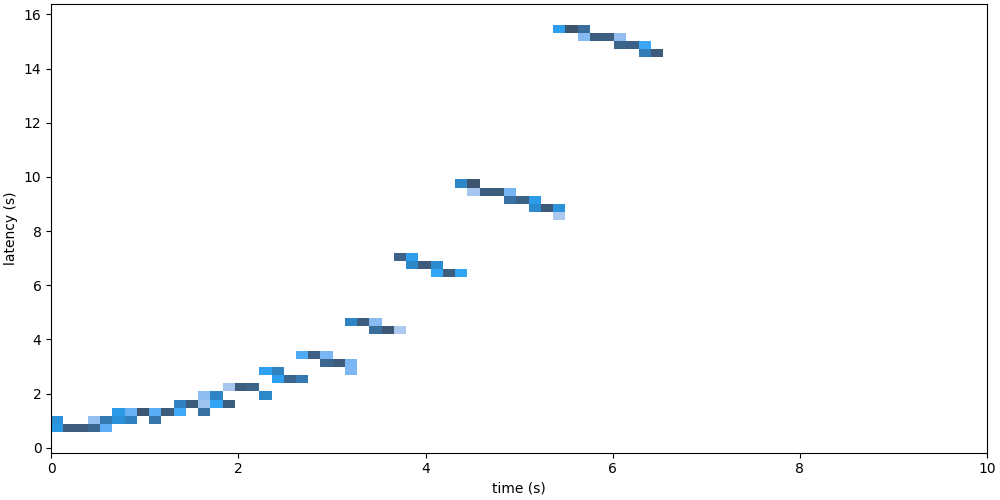
\includegraphics[scale=0.6]{heatmaps/batch_sizes_5_8_1800_4_99999999_timelatencyheatmap.png}
\caption{Heatmap showing exponential growth in latency as the experiment progresses. [add parameters]}
\label{expheatmap}
\end{figure}

This study compares the performance of the system for varying limits on batch sizes (Section \ref{batchsizes}). All experiments were run on a network of 4 nodes.

At lower throughputs where the system is not overloaded, throughput grows linearly with goodput (Figure \ref{throughputgoodputbatch}), as the system is able to respond to all incoming requests, with roughly constant latency throughout an experiment (Figure \ref{stableheatmap}). During this period batches are not filled, so larger throughputs result in larger messages and a linear increase in latency due to increasing serialisation latency (Figure \ref{goodputlatencybatch}). The system is able to reach a higher goodput before being overloaded if it has a larger batch size, as each view results in more commands being committed; this supports our conclusion that batching is an effective optimisation.

Once throughput is increased enough, batches begin to be filled up and the system is overloaded. This results in the goodput flattening out (Figure \ref{throughputgoodputbatch}), as the system cannot handle the volume of requests; commands begin to queue on the nodes and latency increases linearly (Figure \ref{linearheatmap}). For higher batch size limits (especially unlimited), goodput declines once the system is overloaded rather than flattening off. This is because the benefits of larger batches are offset by messages becoming larger, causing increased serialisation latency, which increase view times and lower goodput. For large batch sizes, view times increase exponentially, as shown by the growing vertical gaps between commands being committed in Figure \ref{expheatmap}.

There is a clear trade-off between larger batch sizes that result in more commands being committed, and batches becoming too large and incurring exponential serialisation latency. The optimum for our system appears to be a batch size of around 600 commands, with a maximum goodput of around 900req/s. (Figure \ref{throughputgoodputbatch}).

% There is a trade-off between having larger batches to process more commands, and messages becoming too large and increasing serialisation latency, which is apparent from Figure \ref{throughputgoodputbatch}. With small batch sizes each view only commits a small number of commands, leading to low goodputs; an extreme example of this is a batch size of 1 (equivalent to no batching). As batch sizes increase the goodput reached also increases, with goodput peaking at around 700req/s with a batch size of 300 commands. At this point increasing batch size further causes goodput to decrease due to the increased latency of serialising large messages; each view takes longer so less nodes are committed per second (even though each node contains more commands). When the batch size is unlimited messages grow very large as throughput increases, and increased serialisation latency causes goodput to decline.

% Figure \ref{throughputlatencybatch} shows that latency scales linearly with throughput while the system is not overloaded, that is, when the goodput is within 5\% of the target throughput. This is because larger throughputs result in larger message sizes, and increased latency due to serialisation time. 

\subsection{Node counts} \label{nodecountseval}

\begin{figure}[h!]
\centering
%% Creator: Matplotlib, PGF backend
%%
%% To include the figure in your LaTeX document, write
%%   \input{<filename>.pgf}
%%
%% Make sure the required packages are loaded in your preamble
%%   \usepackage{pgf}
%%
%% Also ensure that all the required font packages are loaded; for instance,
%% the lmodern package is sometimes necessary when using math font.
%%   \usepackage{lmodern}
%%
%% Figures using additional raster images can only be included by \input if
%% they are in the same directory as the main LaTeX file. For loading figures
%% from other directories you can use the `import` package
%%   \usepackage{import}
%%
%% and then include the figures with
%%   \import{<path to file>}{<filename>.pgf}
%%
%% Matplotlib used the following preamble
%%   
%%   \usepackage{fontspec}
%%   \setmainfont{DejaVuSerif.ttf}[Path=\detokenize{/opt/homebrew/lib/python3.10/site-packages/matplotlib/mpl-data/fonts/ttf/}]
%%   \setsansfont{DejaVuSans.ttf}[Path=\detokenize{/opt/homebrew/lib/python3.10/site-packages/matplotlib/mpl-data/fonts/ttf/}]
%%   \setmonofont{DejaVuSansMono.ttf}[Path=\detokenize{/opt/homebrew/lib/python3.10/site-packages/matplotlib/mpl-data/fonts/ttf/}]
%%   \makeatletter\@ifpackageloaded{underscore}{}{\usepackage[strings]{underscore}}\makeatother
%%
\begingroup%
\makeatletter%
\begin{pgfpicture}%
\pgfpathrectangle{\pgfpointorigin}{\pgfqpoint{5.840000in}{5.000000in}}%
\pgfusepath{use as bounding box, clip}%
\begin{pgfscope}%
\pgfsetbuttcap%
\pgfsetmiterjoin%
\definecolor{currentfill}{rgb}{1.000000,1.000000,1.000000}%
\pgfsetfillcolor{currentfill}%
\pgfsetlinewidth{0.000000pt}%
\definecolor{currentstroke}{rgb}{1.000000,1.000000,1.000000}%
\pgfsetstrokecolor{currentstroke}%
\pgfsetdash{}{0pt}%
\pgfpathmoveto{\pgfqpoint{0.000000in}{0.000000in}}%
\pgfpathlineto{\pgfqpoint{5.840000in}{0.000000in}}%
\pgfpathlineto{\pgfqpoint{5.840000in}{5.000000in}}%
\pgfpathlineto{\pgfqpoint{0.000000in}{5.000000in}}%
\pgfpathlineto{\pgfqpoint{0.000000in}{0.000000in}}%
\pgfpathclose%
\pgfusepath{fill}%
\end{pgfscope}%
\begin{pgfscope}%
\pgfsetbuttcap%
\pgfsetmiterjoin%
\definecolor{currentfill}{rgb}{1.000000,1.000000,1.000000}%
\pgfsetfillcolor{currentfill}%
\pgfsetlinewidth{0.000000pt}%
\definecolor{currentstroke}{rgb}{0.000000,0.000000,0.000000}%
\pgfsetstrokecolor{currentstroke}%
\pgfsetstrokeopacity{0.000000}%
\pgfsetdash{}{0pt}%
\pgfpathmoveto{\pgfqpoint{0.776314in}{0.582778in}}%
\pgfpathlineto{\pgfqpoint{4.939579in}{0.582778in}}%
\pgfpathlineto{\pgfqpoint{4.939579in}{4.850000in}}%
\pgfpathlineto{\pgfqpoint{0.776314in}{4.850000in}}%
\pgfpathlineto{\pgfqpoint{0.776314in}{0.582778in}}%
\pgfpathclose%
\pgfusepath{fill}%
\end{pgfscope}%
\begin{pgfscope}%
\pgfpathrectangle{\pgfqpoint{0.776314in}{0.582778in}}{\pgfqpoint{4.163265in}{4.267222in}}%
\pgfusepath{clip}%
\pgfsetbuttcap%
\pgfsetroundjoin%
\definecolor{currentfill}{rgb}{0.003922,0.450980,0.698039}%
\pgfsetfillcolor{currentfill}%
\pgfsetfillopacity{0.200000}%
\pgfsetlinewidth{1.003750pt}%
\definecolor{currentstroke}{rgb}{0.003922,0.450980,0.698039}%
\pgfsetstrokecolor{currentstroke}%
\pgfsetstrokeopacity{0.200000}%
\pgfsetdash{}{0pt}%
\pgfsys@defobject{currentmarker}{\pgfqpoint{0.777355in}{0.583845in}}{\pgfqpoint{4.939579in}{4.847285in}}{%
\pgfpathmoveto{\pgfqpoint{0.777355in}{0.583845in}}%
\pgfpathlineto{\pgfqpoint{0.777355in}{0.583845in}}%
\pgfpathlineto{\pgfqpoint{0.802335in}{0.609448in}}%
\pgfpathlineto{\pgfqpoint{0.828355in}{0.636118in}}%
\pgfpathlineto{\pgfqpoint{0.880396in}{0.689285in}}%
\pgfpathlineto{\pgfqpoint{0.984478in}{0.796017in}}%
\pgfpathlineto{\pgfqpoint{1.192641in}{1.007845in}}%
\pgfpathlineto{\pgfqpoint{1.400804in}{1.220595in}}%
\pgfpathlineto{\pgfqpoint{1.608967in}{1.435263in}}%
\pgfpathlineto{\pgfqpoint{1.817131in}{1.646522in}}%
\pgfpathlineto{\pgfqpoint{2.025294in}{1.860821in}}%
\pgfpathlineto{\pgfqpoint{2.233457in}{2.072155in}}%
\pgfpathlineto{\pgfqpoint{2.441620in}{2.280911in}}%
\pgfpathlineto{\pgfqpoint{2.649784in}{2.502453in}}%
\pgfpathlineto{\pgfqpoint{2.857947in}{2.705141in}}%
\pgfpathlineto{\pgfqpoint{3.066110in}{2.917738in}}%
\pgfpathlineto{\pgfqpoint{3.274273in}{3.136399in}}%
\pgfpathlineto{\pgfqpoint{3.482437in}{3.346771in}}%
\pgfpathlineto{\pgfqpoint{3.690600in}{3.551750in}}%
\pgfpathlineto{\pgfqpoint{3.898763in}{3.754843in}}%
\pgfpathlineto{\pgfqpoint{4.106926in}{3.959256in}}%
\pgfpathlineto{\pgfqpoint{4.315090in}{4.196244in}}%
\pgfpathlineto{\pgfqpoint{4.523253in}{4.402737in}}%
\pgfpathlineto{\pgfqpoint{4.731416in}{4.599384in}}%
\pgfpathlineto{\pgfqpoint{4.939579in}{4.821322in}}%
\pgfpathlineto{\pgfqpoint{4.939579in}{4.847285in}}%
\pgfpathlineto{\pgfqpoint{4.939579in}{4.847285in}}%
\pgfpathlineto{\pgfqpoint{4.731416in}{4.636639in}}%
\pgfpathlineto{\pgfqpoint{4.523253in}{4.420423in}}%
\pgfpathlineto{\pgfqpoint{4.315090in}{4.200886in}}%
\pgfpathlineto{\pgfqpoint{4.106926in}{3.989454in}}%
\pgfpathlineto{\pgfqpoint{3.898763in}{3.772953in}}%
\pgfpathlineto{\pgfqpoint{3.690600in}{3.565066in}}%
\pgfpathlineto{\pgfqpoint{3.482437in}{3.356472in}}%
\pgfpathlineto{\pgfqpoint{3.274273in}{3.143111in}}%
\pgfpathlineto{\pgfqpoint{3.066110in}{2.929750in}}%
\pgfpathlineto{\pgfqpoint{2.857947in}{2.716389in}}%
\pgfpathlineto{\pgfqpoint{2.649784in}{2.503028in}}%
\pgfpathlineto{\pgfqpoint{2.441620in}{2.287882in}}%
\pgfpathlineto{\pgfqpoint{2.233457in}{2.076306in}}%
\pgfpathlineto{\pgfqpoint{2.025294in}{1.861547in}}%
\pgfpathlineto{\pgfqpoint{1.817131in}{1.647636in}}%
\pgfpathlineto{\pgfqpoint{1.608967in}{1.436222in}}%
\pgfpathlineto{\pgfqpoint{1.400804in}{1.222861in}}%
\pgfpathlineto{\pgfqpoint{1.192641in}{1.009500in}}%
\pgfpathlineto{\pgfqpoint{0.984478in}{0.796139in}}%
\pgfpathlineto{\pgfqpoint{0.880396in}{0.689458in}}%
\pgfpathlineto{\pgfqpoint{0.828355in}{0.636118in}}%
\pgfpathlineto{\pgfqpoint{0.802335in}{0.609448in}}%
\pgfpathlineto{\pgfqpoint{0.777355in}{0.583845in}}%
\pgfpathlineto{\pgfqpoint{0.777355in}{0.583845in}}%
\pgfpathclose%
\pgfusepath{stroke,fill}%
}%
\begin{pgfscope}%
\pgfsys@transformshift{0.000000in}{0.000000in}%
\pgfsys@useobject{currentmarker}{}%
\end{pgfscope}%
\end{pgfscope}%
\begin{pgfscope}%
\pgfpathrectangle{\pgfqpoint{0.776314in}{0.582778in}}{\pgfqpoint{4.163265in}{4.267222in}}%
\pgfusepath{clip}%
\pgfsetbuttcap%
\pgfsetroundjoin%
\definecolor{currentfill}{rgb}{0.870588,0.560784,0.019608}%
\pgfsetfillcolor{currentfill}%
\pgfsetfillopacity{0.200000}%
\pgfsetlinewidth{1.003750pt}%
\definecolor{currentstroke}{rgb}{0.870588,0.560784,0.019608}%
\pgfsetstrokecolor{currentstroke}%
\pgfsetstrokeopacity{0.200000}%
\pgfsetdash{}{0pt}%
\pgfsys@defobject{currentmarker}{\pgfqpoint{0.777355in}{0.583845in}}{\pgfqpoint{4.939579in}{2.646855in}}{%
\pgfpathmoveto{\pgfqpoint{0.777355in}{0.583845in}}%
\pgfpathlineto{\pgfqpoint{0.777355in}{0.583845in}}%
\pgfpathlineto{\pgfqpoint{0.802335in}{0.609419in}}%
\pgfpathlineto{\pgfqpoint{0.828355in}{0.636118in}}%
\pgfpathlineto{\pgfqpoint{0.880396in}{0.689406in}}%
\pgfpathlineto{\pgfqpoint{0.984478in}{0.796139in}}%
\pgfpathlineto{\pgfqpoint{1.192641in}{1.009500in}}%
\pgfpathlineto{\pgfqpoint{1.400804in}{1.221913in}}%
\pgfpathlineto{\pgfqpoint{1.608967in}{1.435370in}}%
\pgfpathlineto{\pgfqpoint{1.817131in}{1.643431in}}%
\pgfpathlineto{\pgfqpoint{2.025294in}{1.848823in}}%
\pgfpathlineto{\pgfqpoint{2.233457in}{2.062053in}}%
\pgfpathlineto{\pgfqpoint{2.441620in}{2.270450in}}%
\pgfpathlineto{\pgfqpoint{2.649784in}{2.454465in}}%
\pgfpathlineto{\pgfqpoint{2.857947in}{2.476940in}}%
\pgfpathlineto{\pgfqpoint{3.066110in}{2.192647in}}%
\pgfpathlineto{\pgfqpoint{3.274273in}{2.344683in}}%
\pgfpathlineto{\pgfqpoint{3.482437in}{2.310442in}}%
\pgfpathlineto{\pgfqpoint{3.690600in}{2.315469in}}%
\pgfpathlineto{\pgfqpoint{3.898763in}{2.144824in}}%
\pgfpathlineto{\pgfqpoint{4.106926in}{2.197374in}}%
\pgfpathlineto{\pgfqpoint{4.315090in}{2.203637in}}%
\pgfpathlineto{\pgfqpoint{4.523253in}{2.096988in}}%
\pgfpathlineto{\pgfqpoint{4.731416in}{2.196261in}}%
\pgfpathlineto{\pgfqpoint{4.939579in}{2.088148in}}%
\pgfpathlineto{\pgfqpoint{4.939579in}{2.308405in}}%
\pgfpathlineto{\pgfqpoint{4.939579in}{2.308405in}}%
\pgfpathlineto{\pgfqpoint{4.731416in}{2.259190in}}%
\pgfpathlineto{\pgfqpoint{4.523253in}{2.253129in}}%
\pgfpathlineto{\pgfqpoint{4.315090in}{2.272140in}}%
\pgfpathlineto{\pgfqpoint{4.106926in}{2.347828in}}%
\pgfpathlineto{\pgfqpoint{3.898763in}{2.347474in}}%
\pgfpathlineto{\pgfqpoint{3.690600in}{2.425968in}}%
\pgfpathlineto{\pgfqpoint{3.482437in}{2.470849in}}%
\pgfpathlineto{\pgfqpoint{3.274273in}{2.461408in}}%
\pgfpathlineto{\pgfqpoint{3.066110in}{2.646855in}}%
\pgfpathlineto{\pgfqpoint{2.857947in}{2.611142in}}%
\pgfpathlineto{\pgfqpoint{2.649784in}{2.482632in}}%
\pgfpathlineto{\pgfqpoint{2.441620in}{2.289667in}}%
\pgfpathlineto{\pgfqpoint{2.233457in}{2.076306in}}%
\pgfpathlineto{\pgfqpoint{2.025294in}{1.850793in}}%
\pgfpathlineto{\pgfqpoint{1.817131in}{1.648570in}}%
\pgfpathlineto{\pgfqpoint{1.608967in}{1.436222in}}%
\pgfpathlineto{\pgfqpoint{1.400804in}{1.222861in}}%
\pgfpathlineto{\pgfqpoint{1.192641in}{1.009500in}}%
\pgfpathlineto{\pgfqpoint{0.984478in}{0.796139in}}%
\pgfpathlineto{\pgfqpoint{0.880396in}{0.689458in}}%
\pgfpathlineto{\pgfqpoint{0.828355in}{0.636118in}}%
\pgfpathlineto{\pgfqpoint{0.802335in}{0.609448in}}%
\pgfpathlineto{\pgfqpoint{0.777355in}{0.583845in}}%
\pgfpathlineto{\pgfqpoint{0.777355in}{0.583845in}}%
\pgfpathclose%
\pgfusepath{stroke,fill}%
}%
\begin{pgfscope}%
\pgfsys@transformshift{0.000000in}{0.000000in}%
\pgfsys@useobject{currentmarker}{}%
\end{pgfscope}%
\end{pgfscope}%
\begin{pgfscope}%
\pgfpathrectangle{\pgfqpoint{0.776314in}{0.582778in}}{\pgfqpoint{4.163265in}{4.267222in}}%
\pgfusepath{clip}%
\pgfsetbuttcap%
\pgfsetroundjoin%
\definecolor{currentfill}{rgb}{0.007843,0.619608,0.450980}%
\pgfsetfillcolor{currentfill}%
\pgfsetfillopacity{0.200000}%
\pgfsetlinewidth{1.003750pt}%
\definecolor{currentstroke}{rgb}{0.007843,0.619608,0.450980}%
\pgfsetstrokecolor{currentstroke}%
\pgfsetstrokeopacity{0.200000}%
\pgfsetdash{}{0pt}%
\pgfsys@defobject{currentmarker}{\pgfqpoint{0.777355in}{0.583845in}}{\pgfqpoint{4.939579in}{1.650649in}}{%
\pgfpathmoveto{\pgfqpoint{0.777355in}{0.583845in}}%
\pgfpathlineto{\pgfqpoint{0.777355in}{0.583845in}}%
\pgfpathlineto{\pgfqpoint{0.802335in}{0.609448in}}%
\pgfpathlineto{\pgfqpoint{0.828355in}{0.636118in}}%
\pgfpathlineto{\pgfqpoint{0.880396in}{0.689092in}}%
\pgfpathlineto{\pgfqpoint{0.984478in}{0.795001in}}%
\pgfpathlineto{\pgfqpoint{1.192641in}{1.004840in}}%
\pgfpathlineto{\pgfqpoint{1.400804in}{1.212026in}}%
\pgfpathlineto{\pgfqpoint{1.608967in}{1.405334in}}%
\pgfpathlineto{\pgfqpoint{1.817131in}{1.560525in}}%
\pgfpathlineto{\pgfqpoint{2.025294in}{1.586986in}}%
\pgfpathlineto{\pgfqpoint{2.233457in}{1.518539in}}%
\pgfpathlineto{\pgfqpoint{2.441620in}{1.446476in}}%
\pgfpathlineto{\pgfqpoint{2.649784in}{1.384611in}}%
\pgfpathlineto{\pgfqpoint{2.857947in}{1.359731in}}%
\pgfpathlineto{\pgfqpoint{3.066110in}{1.340767in}}%
\pgfpathlineto{\pgfqpoint{3.274273in}{1.352190in}}%
\pgfpathlineto{\pgfqpoint{3.482437in}{1.338596in}}%
\pgfpathlineto{\pgfqpoint{3.690600in}{1.350507in}}%
\pgfpathlineto{\pgfqpoint{3.898763in}{1.306662in}}%
\pgfpathlineto{\pgfqpoint{4.106926in}{1.316498in}}%
\pgfpathlineto{\pgfqpoint{4.315090in}{1.330574in}}%
\pgfpathlineto{\pgfqpoint{4.523253in}{1.314688in}}%
\pgfpathlineto{\pgfqpoint{4.731416in}{1.317627in}}%
\pgfpathlineto{\pgfqpoint{4.939579in}{1.292674in}}%
\pgfpathlineto{\pgfqpoint{4.939579in}{1.329192in}}%
\pgfpathlineto{\pgfqpoint{4.939579in}{1.329192in}}%
\pgfpathlineto{\pgfqpoint{4.731416in}{1.348511in}}%
\pgfpathlineto{\pgfqpoint{4.523253in}{1.343435in}}%
\pgfpathlineto{\pgfqpoint{4.315090in}{1.350032in}}%
\pgfpathlineto{\pgfqpoint{4.106926in}{1.331857in}}%
\pgfpathlineto{\pgfqpoint{3.898763in}{1.333252in}}%
\pgfpathlineto{\pgfqpoint{3.690600in}{1.355789in}}%
\pgfpathlineto{\pgfqpoint{3.482437in}{1.345611in}}%
\pgfpathlineto{\pgfqpoint{3.274273in}{1.363224in}}%
\pgfpathlineto{\pgfqpoint{3.066110in}{1.368426in}}%
\pgfpathlineto{\pgfqpoint{2.857947in}{1.390592in}}%
\pgfpathlineto{\pgfqpoint{2.649784in}{1.404295in}}%
\pgfpathlineto{\pgfqpoint{2.441620in}{1.509113in}}%
\pgfpathlineto{\pgfqpoint{2.233457in}{1.541141in}}%
\pgfpathlineto{\pgfqpoint{2.025294in}{1.650649in}}%
\pgfpathlineto{\pgfqpoint{1.817131in}{1.617223in}}%
\pgfpathlineto{\pgfqpoint{1.608967in}{1.418080in}}%
\pgfpathlineto{\pgfqpoint{1.400804in}{1.219670in}}%
\pgfpathlineto{\pgfqpoint{1.192641in}{1.009500in}}%
\pgfpathlineto{\pgfqpoint{0.984478in}{0.795975in}}%
\pgfpathlineto{\pgfqpoint{0.880396in}{0.689458in}}%
\pgfpathlineto{\pgfqpoint{0.828355in}{0.636118in}}%
\pgfpathlineto{\pgfqpoint{0.802335in}{0.609448in}}%
\pgfpathlineto{\pgfqpoint{0.777355in}{0.583845in}}%
\pgfpathlineto{\pgfqpoint{0.777355in}{0.583845in}}%
\pgfpathclose%
\pgfusepath{stroke,fill}%
}%
\begin{pgfscope}%
\pgfsys@transformshift{0.000000in}{0.000000in}%
\pgfsys@useobject{currentmarker}{}%
\end{pgfscope}%
\end{pgfscope}%
\begin{pgfscope}%
\pgfpathrectangle{\pgfqpoint{0.776314in}{0.582778in}}{\pgfqpoint{4.163265in}{4.267222in}}%
\pgfusepath{clip}%
\pgfsetbuttcap%
\pgfsetroundjoin%
\definecolor{currentfill}{rgb}{0.835294,0.368627,0.000000}%
\pgfsetfillcolor{currentfill}%
\pgfsetfillopacity{0.200000}%
\pgfsetlinewidth{1.003750pt}%
\definecolor{currentstroke}{rgb}{0.835294,0.368627,0.000000}%
\pgfsetstrokecolor{currentstroke}%
\pgfsetstrokeopacity{0.200000}%
\pgfsetdash{}{0pt}%
\pgfsys@defobject{currentmarker}{\pgfqpoint{0.777355in}{0.583845in}}{\pgfqpoint{4.939579in}{1.239424in}}{%
\pgfpathmoveto{\pgfqpoint{0.777355in}{0.583845in}}%
\pgfpathlineto{\pgfqpoint{0.777355in}{0.583845in}}%
\pgfpathlineto{\pgfqpoint{0.802335in}{0.609448in}}%
\pgfpathlineto{\pgfqpoint{0.828355in}{0.636118in}}%
\pgfpathlineto{\pgfqpoint{0.880396in}{0.689448in}}%
\pgfpathlineto{\pgfqpoint{0.984478in}{0.795187in}}%
\pgfpathlineto{\pgfqpoint{1.192641in}{1.005593in}}%
\pgfpathlineto{\pgfqpoint{1.400804in}{1.190145in}}%
\pgfpathlineto{\pgfqpoint{1.608967in}{1.188582in}}%
\pgfpathlineto{\pgfqpoint{1.817131in}{1.101217in}}%
\pgfpathlineto{\pgfqpoint{2.025294in}{1.081993in}}%
\pgfpathlineto{\pgfqpoint{2.233457in}{1.059514in}}%
\pgfpathlineto{\pgfqpoint{2.441620in}{1.048807in}}%
\pgfpathlineto{\pgfqpoint{2.649784in}{1.046861in}}%
\pgfpathlineto{\pgfqpoint{2.857947in}{1.054474in}}%
\pgfpathlineto{\pgfqpoint{3.066110in}{1.027462in}}%
\pgfpathlineto{\pgfqpoint{3.274273in}{1.055961in}}%
\pgfpathlineto{\pgfqpoint{3.482437in}{1.038027in}}%
\pgfpathlineto{\pgfqpoint{3.690600in}{1.023031in}}%
\pgfpathlineto{\pgfqpoint{3.898763in}{1.041517in}}%
\pgfpathlineto{\pgfqpoint{4.106926in}{1.016707in}}%
\pgfpathlineto{\pgfqpoint{4.315090in}{1.036980in}}%
\pgfpathlineto{\pgfqpoint{4.523253in}{1.020235in}}%
\pgfpathlineto{\pgfqpoint{4.731416in}{1.008330in}}%
\pgfpathlineto{\pgfqpoint{4.939579in}{1.028414in}}%
\pgfpathlineto{\pgfqpoint{4.939579in}{1.037330in}}%
\pgfpathlineto{\pgfqpoint{4.939579in}{1.037330in}}%
\pgfpathlineto{\pgfqpoint{4.731416in}{1.061607in}}%
\pgfpathlineto{\pgfqpoint{4.523253in}{1.051976in}}%
\pgfpathlineto{\pgfqpoint{4.315090in}{1.044672in}}%
\pgfpathlineto{\pgfqpoint{4.106926in}{1.071809in}}%
\pgfpathlineto{\pgfqpoint{3.898763in}{1.045533in}}%
\pgfpathlineto{\pgfqpoint{3.690600in}{1.044251in}}%
\pgfpathlineto{\pgfqpoint{3.482437in}{1.079413in}}%
\pgfpathlineto{\pgfqpoint{3.274273in}{1.082359in}}%
\pgfpathlineto{\pgfqpoint{3.066110in}{1.065800in}}%
\pgfpathlineto{\pgfqpoint{2.857947in}{1.075132in}}%
\pgfpathlineto{\pgfqpoint{2.649784in}{1.064514in}}%
\pgfpathlineto{\pgfqpoint{2.441620in}{1.084806in}}%
\pgfpathlineto{\pgfqpoint{2.233457in}{1.093603in}}%
\pgfpathlineto{\pgfqpoint{2.025294in}{1.096119in}}%
\pgfpathlineto{\pgfqpoint{1.817131in}{1.126273in}}%
\pgfpathlineto{\pgfqpoint{1.608967in}{1.239424in}}%
\pgfpathlineto{\pgfqpoint{1.400804in}{1.200441in}}%
\pgfpathlineto{\pgfqpoint{1.192641in}{1.008969in}}%
\pgfpathlineto{\pgfqpoint{0.984478in}{0.796139in}}%
\pgfpathlineto{\pgfqpoint{0.880396in}{0.689458in}}%
\pgfpathlineto{\pgfqpoint{0.828355in}{0.636118in}}%
\pgfpathlineto{\pgfqpoint{0.802335in}{0.609448in}}%
\pgfpathlineto{\pgfqpoint{0.777355in}{0.583845in}}%
\pgfpathlineto{\pgfqpoint{0.777355in}{0.583845in}}%
\pgfpathclose%
\pgfusepath{stroke,fill}%
}%
\begin{pgfscope}%
\pgfsys@transformshift{0.000000in}{0.000000in}%
\pgfsys@useobject{currentmarker}{}%
\end{pgfscope}%
\end{pgfscope}%
\begin{pgfscope}%
\pgfpathrectangle{\pgfqpoint{0.776314in}{0.582778in}}{\pgfqpoint{4.163265in}{4.267222in}}%
\pgfusepath{clip}%
\pgfsetbuttcap%
\pgfsetroundjoin%
\definecolor{currentfill}{rgb}{0.800000,0.470588,0.737255}%
\pgfsetfillcolor{currentfill}%
\pgfsetfillopacity{0.200000}%
\pgfsetlinewidth{1.003750pt}%
\definecolor{currentstroke}{rgb}{0.800000,0.470588,0.737255}%
\pgfsetstrokecolor{currentstroke}%
\pgfsetstrokeopacity{0.200000}%
\pgfsetdash{}{0pt}%
\pgfsys@defobject{currentmarker}{\pgfqpoint{0.777355in}{0.583845in}}{\pgfqpoint{4.939579in}{1.062390in}}{%
\pgfpathmoveto{\pgfqpoint{0.777355in}{0.583845in}}%
\pgfpathlineto{\pgfqpoint{0.777355in}{0.583845in}}%
\pgfpathlineto{\pgfqpoint{0.802335in}{0.609448in}}%
\pgfpathlineto{\pgfqpoint{0.828355in}{0.636118in}}%
\pgfpathlineto{\pgfqpoint{0.880396in}{0.689458in}}%
\pgfpathlineto{\pgfqpoint{0.984478in}{0.796139in}}%
\pgfpathlineto{\pgfqpoint{1.192641in}{0.997045in}}%
\pgfpathlineto{\pgfqpoint{1.400804in}{1.038514in}}%
\pgfpathlineto{\pgfqpoint{1.608967in}{0.981191in}}%
\pgfpathlineto{\pgfqpoint{1.817131in}{0.959308in}}%
\pgfpathlineto{\pgfqpoint{2.025294in}{0.969021in}}%
\pgfpathlineto{\pgfqpoint{2.233457in}{0.937423in}}%
\pgfpathlineto{\pgfqpoint{2.441620in}{0.956981in}}%
\pgfpathlineto{\pgfqpoint{2.649784in}{0.954590in}}%
\pgfpathlineto{\pgfqpoint{2.857947in}{0.922885in}}%
\pgfpathlineto{\pgfqpoint{3.066110in}{0.946566in}}%
\pgfpathlineto{\pgfqpoint{3.274273in}{0.940952in}}%
\pgfpathlineto{\pgfqpoint{3.482437in}{0.938011in}}%
\pgfpathlineto{\pgfqpoint{3.690600in}{0.917226in}}%
\pgfpathlineto{\pgfqpoint{3.898763in}{0.924350in}}%
\pgfpathlineto{\pgfqpoint{4.106926in}{0.930172in}}%
\pgfpathlineto{\pgfqpoint{4.315090in}{0.912600in}}%
\pgfpathlineto{\pgfqpoint{4.523253in}{0.926650in}}%
\pgfpathlineto{\pgfqpoint{4.731416in}{0.918982in}}%
\pgfpathlineto{\pgfqpoint{4.939579in}{0.926503in}}%
\pgfpathlineto{\pgfqpoint{4.939579in}{0.938031in}}%
\pgfpathlineto{\pgfqpoint{4.939579in}{0.938031in}}%
\pgfpathlineto{\pgfqpoint{4.731416in}{0.936190in}}%
\pgfpathlineto{\pgfqpoint{4.523253in}{0.932038in}}%
\pgfpathlineto{\pgfqpoint{4.315090in}{0.944383in}}%
\pgfpathlineto{\pgfqpoint{4.106926in}{0.942104in}}%
\pgfpathlineto{\pgfqpoint{3.898763in}{0.955241in}}%
\pgfpathlineto{\pgfqpoint{3.690600in}{0.942451in}}%
\pgfpathlineto{\pgfqpoint{3.482437in}{0.952655in}}%
\pgfpathlineto{\pgfqpoint{3.274273in}{0.953879in}}%
\pgfpathlineto{\pgfqpoint{3.066110in}{0.966292in}}%
\pgfpathlineto{\pgfqpoint{2.857947in}{0.969547in}}%
\pgfpathlineto{\pgfqpoint{2.649784in}{0.958659in}}%
\pgfpathlineto{\pgfqpoint{2.441620in}{0.969073in}}%
\pgfpathlineto{\pgfqpoint{2.233457in}{0.976483in}}%
\pgfpathlineto{\pgfqpoint{2.025294in}{0.975626in}}%
\pgfpathlineto{\pgfqpoint{1.817131in}{0.978438in}}%
\pgfpathlineto{\pgfqpoint{1.608967in}{1.005816in}}%
\pgfpathlineto{\pgfqpoint{1.400804in}{1.062390in}}%
\pgfpathlineto{\pgfqpoint{1.192641in}{1.004329in}}%
\pgfpathlineto{\pgfqpoint{0.984478in}{0.796139in}}%
\pgfpathlineto{\pgfqpoint{0.880396in}{0.689458in}}%
\pgfpathlineto{\pgfqpoint{0.828355in}{0.636118in}}%
\pgfpathlineto{\pgfqpoint{0.802335in}{0.609448in}}%
\pgfpathlineto{\pgfqpoint{0.777355in}{0.583845in}}%
\pgfpathlineto{\pgfqpoint{0.777355in}{0.583845in}}%
\pgfpathclose%
\pgfusepath{stroke,fill}%
}%
\begin{pgfscope}%
\pgfsys@transformshift{0.000000in}{0.000000in}%
\pgfsys@useobject{currentmarker}{}%
\end{pgfscope}%
\end{pgfscope}%
\begin{pgfscope}%
\pgfpathrectangle{\pgfqpoint{0.776314in}{0.582778in}}{\pgfqpoint{4.163265in}{4.267222in}}%
\pgfusepath{clip}%
\pgfsetbuttcap%
\pgfsetroundjoin%
\definecolor{currentfill}{rgb}{0.792157,0.568627,0.380392}%
\pgfsetfillcolor{currentfill}%
\pgfsetfillopacity{0.200000}%
\pgfsetlinewidth{1.003750pt}%
\definecolor{currentstroke}{rgb}{0.792157,0.568627,0.380392}%
\pgfsetstrokecolor{currentstroke}%
\pgfsetstrokeopacity{0.200000}%
\pgfsetdash{}{0pt}%
\pgfsys@defobject{currentmarker}{\pgfqpoint{0.777355in}{0.583845in}}{\pgfqpoint{4.939579in}{0.981977in}}{%
\pgfpathmoveto{\pgfqpoint{0.777355in}{0.583845in}}%
\pgfpathlineto{\pgfqpoint{0.777355in}{0.583845in}}%
\pgfpathlineto{\pgfqpoint{0.802335in}{0.609448in}}%
\pgfpathlineto{\pgfqpoint{0.828355in}{0.636118in}}%
\pgfpathlineto{\pgfqpoint{0.880396in}{0.689458in}}%
\pgfpathlineto{\pgfqpoint{0.984478in}{0.796139in}}%
\pgfpathlineto{\pgfqpoint{1.192641in}{0.967107in}}%
\pgfpathlineto{\pgfqpoint{1.400804in}{0.907165in}}%
\pgfpathlineto{\pgfqpoint{1.608967in}{0.865923in}}%
\pgfpathlineto{\pgfqpoint{1.817131in}{0.878169in}}%
\pgfpathlineto{\pgfqpoint{2.025294in}{0.873357in}}%
\pgfpathlineto{\pgfqpoint{2.233457in}{0.878627in}}%
\pgfpathlineto{\pgfqpoint{2.441620in}{0.869986in}}%
\pgfpathlineto{\pgfqpoint{2.649784in}{0.865009in}}%
\pgfpathlineto{\pgfqpoint{2.857947in}{0.860830in}}%
\pgfpathlineto{\pgfqpoint{3.066110in}{0.861438in}}%
\pgfpathlineto{\pgfqpoint{3.274273in}{0.857353in}}%
\pgfpathlineto{\pgfqpoint{3.482437in}{0.861800in}}%
\pgfpathlineto{\pgfqpoint{3.690600in}{0.861963in}}%
\pgfpathlineto{\pgfqpoint{3.898763in}{0.871036in}}%
\pgfpathlineto{\pgfqpoint{4.106926in}{0.859813in}}%
\pgfpathlineto{\pgfqpoint{4.315090in}{0.836024in}}%
\pgfpathlineto{\pgfqpoint{4.523253in}{0.868875in}}%
\pgfpathlineto{\pgfqpoint{4.731416in}{0.850404in}}%
\pgfpathlineto{\pgfqpoint{4.939579in}{0.847171in}}%
\pgfpathlineto{\pgfqpoint{4.939579in}{0.866197in}}%
\pgfpathlineto{\pgfqpoint{4.939579in}{0.866197in}}%
\pgfpathlineto{\pgfqpoint{4.731416in}{0.863733in}}%
\pgfpathlineto{\pgfqpoint{4.523253in}{0.870987in}}%
\pgfpathlineto{\pgfqpoint{4.315090in}{0.858624in}}%
\pgfpathlineto{\pgfqpoint{4.106926in}{0.873470in}}%
\pgfpathlineto{\pgfqpoint{3.898763in}{0.881068in}}%
\pgfpathlineto{\pgfqpoint{3.690600in}{0.866542in}}%
\pgfpathlineto{\pgfqpoint{3.482437in}{0.872361in}}%
\pgfpathlineto{\pgfqpoint{3.274273in}{0.876018in}}%
\pgfpathlineto{\pgfqpoint{3.066110in}{0.873015in}}%
\pgfpathlineto{\pgfqpoint{2.857947in}{0.881247in}}%
\pgfpathlineto{\pgfqpoint{2.649784in}{0.876564in}}%
\pgfpathlineto{\pgfqpoint{2.441620in}{0.882934in}}%
\pgfpathlineto{\pgfqpoint{2.233457in}{0.887404in}}%
\pgfpathlineto{\pgfqpoint{2.025294in}{0.891092in}}%
\pgfpathlineto{\pgfqpoint{1.817131in}{0.885017in}}%
\pgfpathlineto{\pgfqpoint{1.608967in}{0.899987in}}%
\pgfpathlineto{\pgfqpoint{1.400804in}{0.920507in}}%
\pgfpathlineto{\pgfqpoint{1.192641in}{0.981977in}}%
\pgfpathlineto{\pgfqpoint{0.984478in}{0.796139in}}%
\pgfpathlineto{\pgfqpoint{0.880396in}{0.689458in}}%
\pgfpathlineto{\pgfqpoint{0.828355in}{0.636118in}}%
\pgfpathlineto{\pgfqpoint{0.802335in}{0.609448in}}%
\pgfpathlineto{\pgfqpoint{0.777355in}{0.583845in}}%
\pgfpathlineto{\pgfqpoint{0.777355in}{0.583845in}}%
\pgfpathclose%
\pgfusepath{stroke,fill}%
}%
\begin{pgfscope}%
\pgfsys@transformshift{0.000000in}{0.000000in}%
\pgfsys@useobject{currentmarker}{}%
\end{pgfscope}%
\end{pgfscope}%
\begin{pgfscope}%
\pgfsetbuttcap%
\pgfsetroundjoin%
\definecolor{currentfill}{rgb}{0.000000,0.000000,0.000000}%
\pgfsetfillcolor{currentfill}%
\pgfsetlinewidth{0.803000pt}%
\definecolor{currentstroke}{rgb}{0.000000,0.000000,0.000000}%
\pgfsetstrokecolor{currentstroke}%
\pgfsetdash{}{0pt}%
\pgfsys@defobject{currentmarker}{\pgfqpoint{0.000000in}{-0.048611in}}{\pgfqpoint{0.000000in}{0.000000in}}{%
\pgfpathmoveto{\pgfqpoint{0.000000in}{0.000000in}}%
\pgfpathlineto{\pgfqpoint{0.000000in}{-0.048611in}}%
\pgfusepath{stroke,fill}%
}%
\begin{pgfscope}%
\pgfsys@transformshift{0.776314in}{0.582778in}%
\pgfsys@useobject{currentmarker}{}%
\end{pgfscope}%
\end{pgfscope}%
\begin{pgfscope}%
\definecolor{textcolor}{rgb}{0.000000,0.000000,0.000000}%
\pgfsetstrokecolor{textcolor}%
\pgfsetfillcolor{textcolor}%
\pgftext[x=0.776314in,y=0.485556in,,top]{\color{textcolor}\sffamily\fontsize{10.000000}{12.000000}\selectfont 0}%
\end{pgfscope}%
\begin{pgfscope}%
\pgfsetbuttcap%
\pgfsetroundjoin%
\definecolor{currentfill}{rgb}{0.000000,0.000000,0.000000}%
\pgfsetfillcolor{currentfill}%
\pgfsetlinewidth{0.803000pt}%
\definecolor{currentstroke}{rgb}{0.000000,0.000000,0.000000}%
\pgfsetstrokecolor{currentstroke}%
\pgfsetdash{}{0pt}%
\pgfsys@defobject{currentmarker}{\pgfqpoint{0.000000in}{-0.048611in}}{\pgfqpoint{0.000000in}{0.000000in}}{%
\pgfpathmoveto{\pgfqpoint{0.000000in}{0.000000in}}%
\pgfpathlineto{\pgfqpoint{0.000000in}{-0.048611in}}%
\pgfusepath{stroke,fill}%
}%
\begin{pgfscope}%
\pgfsys@transformshift{1.296723in}{0.582778in}%
\pgfsys@useobject{currentmarker}{}%
\end{pgfscope}%
\end{pgfscope}%
\begin{pgfscope}%
\definecolor{textcolor}{rgb}{0.000000,0.000000,0.000000}%
\pgfsetstrokecolor{textcolor}%
\pgfsetfillcolor{textcolor}%
\pgftext[x=1.296723in,y=0.485556in,,top]{\color{textcolor}\sffamily\fontsize{10.000000}{12.000000}\selectfont 500}%
\end{pgfscope}%
\begin{pgfscope}%
\pgfsetbuttcap%
\pgfsetroundjoin%
\definecolor{currentfill}{rgb}{0.000000,0.000000,0.000000}%
\pgfsetfillcolor{currentfill}%
\pgfsetlinewidth{0.803000pt}%
\definecolor{currentstroke}{rgb}{0.000000,0.000000,0.000000}%
\pgfsetstrokecolor{currentstroke}%
\pgfsetdash{}{0pt}%
\pgfsys@defobject{currentmarker}{\pgfqpoint{0.000000in}{-0.048611in}}{\pgfqpoint{0.000000in}{0.000000in}}{%
\pgfpathmoveto{\pgfqpoint{0.000000in}{0.000000in}}%
\pgfpathlineto{\pgfqpoint{0.000000in}{-0.048611in}}%
\pgfusepath{stroke,fill}%
}%
\begin{pgfscope}%
\pgfsys@transformshift{1.817131in}{0.582778in}%
\pgfsys@useobject{currentmarker}{}%
\end{pgfscope}%
\end{pgfscope}%
\begin{pgfscope}%
\definecolor{textcolor}{rgb}{0.000000,0.000000,0.000000}%
\pgfsetstrokecolor{textcolor}%
\pgfsetfillcolor{textcolor}%
\pgftext[x=1.817131in,y=0.485556in,,top]{\color{textcolor}\sffamily\fontsize{10.000000}{12.000000}\selectfont 1000}%
\end{pgfscope}%
\begin{pgfscope}%
\pgfsetbuttcap%
\pgfsetroundjoin%
\definecolor{currentfill}{rgb}{0.000000,0.000000,0.000000}%
\pgfsetfillcolor{currentfill}%
\pgfsetlinewidth{0.803000pt}%
\definecolor{currentstroke}{rgb}{0.000000,0.000000,0.000000}%
\pgfsetstrokecolor{currentstroke}%
\pgfsetdash{}{0pt}%
\pgfsys@defobject{currentmarker}{\pgfqpoint{0.000000in}{-0.048611in}}{\pgfqpoint{0.000000in}{0.000000in}}{%
\pgfpathmoveto{\pgfqpoint{0.000000in}{0.000000in}}%
\pgfpathlineto{\pgfqpoint{0.000000in}{-0.048611in}}%
\pgfusepath{stroke,fill}%
}%
\begin{pgfscope}%
\pgfsys@transformshift{2.337539in}{0.582778in}%
\pgfsys@useobject{currentmarker}{}%
\end{pgfscope}%
\end{pgfscope}%
\begin{pgfscope}%
\definecolor{textcolor}{rgb}{0.000000,0.000000,0.000000}%
\pgfsetstrokecolor{textcolor}%
\pgfsetfillcolor{textcolor}%
\pgftext[x=2.337539in,y=0.485556in,,top]{\color{textcolor}\sffamily\fontsize{10.000000}{12.000000}\selectfont 1500}%
\end{pgfscope}%
\begin{pgfscope}%
\pgfsetbuttcap%
\pgfsetroundjoin%
\definecolor{currentfill}{rgb}{0.000000,0.000000,0.000000}%
\pgfsetfillcolor{currentfill}%
\pgfsetlinewidth{0.803000pt}%
\definecolor{currentstroke}{rgb}{0.000000,0.000000,0.000000}%
\pgfsetstrokecolor{currentstroke}%
\pgfsetdash{}{0pt}%
\pgfsys@defobject{currentmarker}{\pgfqpoint{0.000000in}{-0.048611in}}{\pgfqpoint{0.000000in}{0.000000in}}{%
\pgfpathmoveto{\pgfqpoint{0.000000in}{0.000000in}}%
\pgfpathlineto{\pgfqpoint{0.000000in}{-0.048611in}}%
\pgfusepath{stroke,fill}%
}%
\begin{pgfscope}%
\pgfsys@transformshift{2.857947in}{0.582778in}%
\pgfsys@useobject{currentmarker}{}%
\end{pgfscope}%
\end{pgfscope}%
\begin{pgfscope}%
\definecolor{textcolor}{rgb}{0.000000,0.000000,0.000000}%
\pgfsetstrokecolor{textcolor}%
\pgfsetfillcolor{textcolor}%
\pgftext[x=2.857947in,y=0.485556in,,top]{\color{textcolor}\sffamily\fontsize{10.000000}{12.000000}\selectfont 2000}%
\end{pgfscope}%
\begin{pgfscope}%
\pgfsetbuttcap%
\pgfsetroundjoin%
\definecolor{currentfill}{rgb}{0.000000,0.000000,0.000000}%
\pgfsetfillcolor{currentfill}%
\pgfsetlinewidth{0.803000pt}%
\definecolor{currentstroke}{rgb}{0.000000,0.000000,0.000000}%
\pgfsetstrokecolor{currentstroke}%
\pgfsetdash{}{0pt}%
\pgfsys@defobject{currentmarker}{\pgfqpoint{0.000000in}{-0.048611in}}{\pgfqpoint{0.000000in}{0.000000in}}{%
\pgfpathmoveto{\pgfqpoint{0.000000in}{0.000000in}}%
\pgfpathlineto{\pgfqpoint{0.000000in}{-0.048611in}}%
\pgfusepath{stroke,fill}%
}%
\begin{pgfscope}%
\pgfsys@transformshift{3.378355in}{0.582778in}%
\pgfsys@useobject{currentmarker}{}%
\end{pgfscope}%
\end{pgfscope}%
\begin{pgfscope}%
\definecolor{textcolor}{rgb}{0.000000,0.000000,0.000000}%
\pgfsetstrokecolor{textcolor}%
\pgfsetfillcolor{textcolor}%
\pgftext[x=3.378355in,y=0.485556in,,top]{\color{textcolor}\sffamily\fontsize{10.000000}{12.000000}\selectfont 2500}%
\end{pgfscope}%
\begin{pgfscope}%
\pgfsetbuttcap%
\pgfsetroundjoin%
\definecolor{currentfill}{rgb}{0.000000,0.000000,0.000000}%
\pgfsetfillcolor{currentfill}%
\pgfsetlinewidth{0.803000pt}%
\definecolor{currentstroke}{rgb}{0.000000,0.000000,0.000000}%
\pgfsetstrokecolor{currentstroke}%
\pgfsetdash{}{0pt}%
\pgfsys@defobject{currentmarker}{\pgfqpoint{0.000000in}{-0.048611in}}{\pgfqpoint{0.000000in}{0.000000in}}{%
\pgfpathmoveto{\pgfqpoint{0.000000in}{0.000000in}}%
\pgfpathlineto{\pgfqpoint{0.000000in}{-0.048611in}}%
\pgfusepath{stroke,fill}%
}%
\begin{pgfscope}%
\pgfsys@transformshift{3.898763in}{0.582778in}%
\pgfsys@useobject{currentmarker}{}%
\end{pgfscope}%
\end{pgfscope}%
\begin{pgfscope}%
\definecolor{textcolor}{rgb}{0.000000,0.000000,0.000000}%
\pgfsetstrokecolor{textcolor}%
\pgfsetfillcolor{textcolor}%
\pgftext[x=3.898763in,y=0.485556in,,top]{\color{textcolor}\sffamily\fontsize{10.000000}{12.000000}\selectfont 3000}%
\end{pgfscope}%
\begin{pgfscope}%
\pgfsetbuttcap%
\pgfsetroundjoin%
\definecolor{currentfill}{rgb}{0.000000,0.000000,0.000000}%
\pgfsetfillcolor{currentfill}%
\pgfsetlinewidth{0.803000pt}%
\definecolor{currentstroke}{rgb}{0.000000,0.000000,0.000000}%
\pgfsetstrokecolor{currentstroke}%
\pgfsetdash{}{0pt}%
\pgfsys@defobject{currentmarker}{\pgfqpoint{0.000000in}{-0.048611in}}{\pgfqpoint{0.000000in}{0.000000in}}{%
\pgfpathmoveto{\pgfqpoint{0.000000in}{0.000000in}}%
\pgfpathlineto{\pgfqpoint{0.000000in}{-0.048611in}}%
\pgfusepath{stroke,fill}%
}%
\begin{pgfscope}%
\pgfsys@transformshift{4.419171in}{0.582778in}%
\pgfsys@useobject{currentmarker}{}%
\end{pgfscope}%
\end{pgfscope}%
\begin{pgfscope}%
\definecolor{textcolor}{rgb}{0.000000,0.000000,0.000000}%
\pgfsetstrokecolor{textcolor}%
\pgfsetfillcolor{textcolor}%
\pgftext[x=4.419171in,y=0.485556in,,top]{\color{textcolor}\sffamily\fontsize{10.000000}{12.000000}\selectfont 3500}%
\end{pgfscope}%
\begin{pgfscope}%
\pgfsetbuttcap%
\pgfsetroundjoin%
\definecolor{currentfill}{rgb}{0.000000,0.000000,0.000000}%
\pgfsetfillcolor{currentfill}%
\pgfsetlinewidth{0.803000pt}%
\definecolor{currentstroke}{rgb}{0.000000,0.000000,0.000000}%
\pgfsetstrokecolor{currentstroke}%
\pgfsetdash{}{0pt}%
\pgfsys@defobject{currentmarker}{\pgfqpoint{0.000000in}{-0.048611in}}{\pgfqpoint{0.000000in}{0.000000in}}{%
\pgfpathmoveto{\pgfqpoint{0.000000in}{0.000000in}}%
\pgfpathlineto{\pgfqpoint{0.000000in}{-0.048611in}}%
\pgfusepath{stroke,fill}%
}%
\begin{pgfscope}%
\pgfsys@transformshift{4.939579in}{0.582778in}%
\pgfsys@useobject{currentmarker}{}%
\end{pgfscope}%
\end{pgfscope}%
\begin{pgfscope}%
\definecolor{textcolor}{rgb}{0.000000,0.000000,0.000000}%
\pgfsetstrokecolor{textcolor}%
\pgfsetfillcolor{textcolor}%
\pgftext[x=4.939579in,y=0.485556in,,top]{\color{textcolor}\sffamily\fontsize{10.000000}{12.000000}\selectfont 4000}%
\end{pgfscope}%
\begin{pgfscope}%
\definecolor{textcolor}{rgb}{0.000000,0.000000,0.000000}%
\pgfsetstrokecolor{textcolor}%
\pgfsetfillcolor{textcolor}%
\pgftext[x=2.857947in,y=0.295587in,,top]{\color{textcolor}\sffamily\fontsize{10.000000}{12.000000}\selectfont throughput (req/s)}%
\end{pgfscope}%
\begin{pgfscope}%
\pgfsetbuttcap%
\pgfsetroundjoin%
\definecolor{currentfill}{rgb}{0.000000,0.000000,0.000000}%
\pgfsetfillcolor{currentfill}%
\pgfsetlinewidth{0.803000pt}%
\definecolor{currentstroke}{rgb}{0.000000,0.000000,0.000000}%
\pgfsetstrokecolor{currentstroke}%
\pgfsetdash{}{0pt}%
\pgfsys@defobject{currentmarker}{\pgfqpoint{-0.048611in}{0.000000in}}{\pgfqpoint{-0.000000in}{0.000000in}}{%
\pgfpathmoveto{\pgfqpoint{-0.000000in}{0.000000in}}%
\pgfpathlineto{\pgfqpoint{-0.048611in}{0.000000in}}%
\pgfusepath{stroke,fill}%
}%
\begin{pgfscope}%
\pgfsys@transformshift{0.776314in}{0.582778in}%
\pgfsys@useobject{currentmarker}{}%
\end{pgfscope}%
\end{pgfscope}%
\begin{pgfscope}%
\definecolor{textcolor}{rgb}{0.000000,0.000000,0.000000}%
\pgfsetstrokecolor{textcolor}%
\pgfsetfillcolor{textcolor}%
\pgftext[x=0.590727in, y=0.530016in, left, base]{\color{textcolor}\sffamily\fontsize{10.000000}{12.000000}\selectfont 0}%
\end{pgfscope}%
\begin{pgfscope}%
\pgfsetbuttcap%
\pgfsetroundjoin%
\definecolor{currentfill}{rgb}{0.000000,0.000000,0.000000}%
\pgfsetfillcolor{currentfill}%
\pgfsetlinewidth{0.803000pt}%
\definecolor{currentstroke}{rgb}{0.000000,0.000000,0.000000}%
\pgfsetstrokecolor{currentstroke}%
\pgfsetdash{}{0pt}%
\pgfsys@defobject{currentmarker}{\pgfqpoint{-0.048611in}{0.000000in}}{\pgfqpoint{-0.000000in}{0.000000in}}{%
\pgfpathmoveto{\pgfqpoint{-0.000000in}{0.000000in}}%
\pgfpathlineto{\pgfqpoint{-0.048611in}{0.000000in}}%
\pgfusepath{stroke,fill}%
}%
\begin{pgfscope}%
\pgfsys@transformshift{0.776314in}{1.116181in}%
\pgfsys@useobject{currentmarker}{}%
\end{pgfscope}%
\end{pgfscope}%
\begin{pgfscope}%
\definecolor{textcolor}{rgb}{0.000000,0.000000,0.000000}%
\pgfsetstrokecolor{textcolor}%
\pgfsetfillcolor{textcolor}%
\pgftext[x=0.413996in, y=1.063419in, left, base]{\color{textcolor}\sffamily\fontsize{10.000000}{12.000000}\selectfont 500}%
\end{pgfscope}%
\begin{pgfscope}%
\pgfsetbuttcap%
\pgfsetroundjoin%
\definecolor{currentfill}{rgb}{0.000000,0.000000,0.000000}%
\pgfsetfillcolor{currentfill}%
\pgfsetlinewidth{0.803000pt}%
\definecolor{currentstroke}{rgb}{0.000000,0.000000,0.000000}%
\pgfsetstrokecolor{currentstroke}%
\pgfsetdash{}{0pt}%
\pgfsys@defobject{currentmarker}{\pgfqpoint{-0.048611in}{0.000000in}}{\pgfqpoint{-0.000000in}{0.000000in}}{%
\pgfpathmoveto{\pgfqpoint{-0.000000in}{0.000000in}}%
\pgfpathlineto{\pgfqpoint{-0.048611in}{0.000000in}}%
\pgfusepath{stroke,fill}%
}%
\begin{pgfscope}%
\pgfsys@transformshift{0.776314in}{1.649583in}%
\pgfsys@useobject{currentmarker}{}%
\end{pgfscope}%
\end{pgfscope}%
\begin{pgfscope}%
\definecolor{textcolor}{rgb}{0.000000,0.000000,0.000000}%
\pgfsetstrokecolor{textcolor}%
\pgfsetfillcolor{textcolor}%
\pgftext[x=0.325631in, y=1.596822in, left, base]{\color{textcolor}\sffamily\fontsize{10.000000}{12.000000}\selectfont 1000}%
\end{pgfscope}%
\begin{pgfscope}%
\pgfsetbuttcap%
\pgfsetroundjoin%
\definecolor{currentfill}{rgb}{0.000000,0.000000,0.000000}%
\pgfsetfillcolor{currentfill}%
\pgfsetlinewidth{0.803000pt}%
\definecolor{currentstroke}{rgb}{0.000000,0.000000,0.000000}%
\pgfsetstrokecolor{currentstroke}%
\pgfsetdash{}{0pt}%
\pgfsys@defobject{currentmarker}{\pgfqpoint{-0.048611in}{0.000000in}}{\pgfqpoint{-0.000000in}{0.000000in}}{%
\pgfpathmoveto{\pgfqpoint{-0.000000in}{0.000000in}}%
\pgfpathlineto{\pgfqpoint{-0.048611in}{0.000000in}}%
\pgfusepath{stroke,fill}%
}%
\begin{pgfscope}%
\pgfsys@transformshift{0.776314in}{2.182986in}%
\pgfsys@useobject{currentmarker}{}%
\end{pgfscope}%
\end{pgfscope}%
\begin{pgfscope}%
\definecolor{textcolor}{rgb}{0.000000,0.000000,0.000000}%
\pgfsetstrokecolor{textcolor}%
\pgfsetfillcolor{textcolor}%
\pgftext[x=0.325631in, y=2.130225in, left, base]{\color{textcolor}\sffamily\fontsize{10.000000}{12.000000}\selectfont 1500}%
\end{pgfscope}%
\begin{pgfscope}%
\pgfsetbuttcap%
\pgfsetroundjoin%
\definecolor{currentfill}{rgb}{0.000000,0.000000,0.000000}%
\pgfsetfillcolor{currentfill}%
\pgfsetlinewidth{0.803000pt}%
\definecolor{currentstroke}{rgb}{0.000000,0.000000,0.000000}%
\pgfsetstrokecolor{currentstroke}%
\pgfsetdash{}{0pt}%
\pgfsys@defobject{currentmarker}{\pgfqpoint{-0.048611in}{0.000000in}}{\pgfqpoint{-0.000000in}{0.000000in}}{%
\pgfpathmoveto{\pgfqpoint{-0.000000in}{0.000000in}}%
\pgfpathlineto{\pgfqpoint{-0.048611in}{0.000000in}}%
\pgfusepath{stroke,fill}%
}%
\begin{pgfscope}%
\pgfsys@transformshift{0.776314in}{2.716389in}%
\pgfsys@useobject{currentmarker}{}%
\end{pgfscope}%
\end{pgfscope}%
\begin{pgfscope}%
\definecolor{textcolor}{rgb}{0.000000,0.000000,0.000000}%
\pgfsetstrokecolor{textcolor}%
\pgfsetfillcolor{textcolor}%
\pgftext[x=0.325631in, y=2.663627in, left, base]{\color{textcolor}\sffamily\fontsize{10.000000}{12.000000}\selectfont 2000}%
\end{pgfscope}%
\begin{pgfscope}%
\pgfsetbuttcap%
\pgfsetroundjoin%
\definecolor{currentfill}{rgb}{0.000000,0.000000,0.000000}%
\pgfsetfillcolor{currentfill}%
\pgfsetlinewidth{0.803000pt}%
\definecolor{currentstroke}{rgb}{0.000000,0.000000,0.000000}%
\pgfsetstrokecolor{currentstroke}%
\pgfsetdash{}{0pt}%
\pgfsys@defobject{currentmarker}{\pgfqpoint{-0.048611in}{0.000000in}}{\pgfqpoint{-0.000000in}{0.000000in}}{%
\pgfpathmoveto{\pgfqpoint{-0.000000in}{0.000000in}}%
\pgfpathlineto{\pgfqpoint{-0.048611in}{0.000000in}}%
\pgfusepath{stroke,fill}%
}%
\begin{pgfscope}%
\pgfsys@transformshift{0.776314in}{3.249792in}%
\pgfsys@useobject{currentmarker}{}%
\end{pgfscope}%
\end{pgfscope}%
\begin{pgfscope}%
\definecolor{textcolor}{rgb}{0.000000,0.000000,0.000000}%
\pgfsetstrokecolor{textcolor}%
\pgfsetfillcolor{textcolor}%
\pgftext[x=0.325631in, y=3.197030in, left, base]{\color{textcolor}\sffamily\fontsize{10.000000}{12.000000}\selectfont 2500}%
\end{pgfscope}%
\begin{pgfscope}%
\pgfsetbuttcap%
\pgfsetroundjoin%
\definecolor{currentfill}{rgb}{0.000000,0.000000,0.000000}%
\pgfsetfillcolor{currentfill}%
\pgfsetlinewidth{0.803000pt}%
\definecolor{currentstroke}{rgb}{0.000000,0.000000,0.000000}%
\pgfsetstrokecolor{currentstroke}%
\pgfsetdash{}{0pt}%
\pgfsys@defobject{currentmarker}{\pgfqpoint{-0.048611in}{0.000000in}}{\pgfqpoint{-0.000000in}{0.000000in}}{%
\pgfpathmoveto{\pgfqpoint{-0.000000in}{0.000000in}}%
\pgfpathlineto{\pgfqpoint{-0.048611in}{0.000000in}}%
\pgfusepath{stroke,fill}%
}%
\begin{pgfscope}%
\pgfsys@transformshift{0.776314in}{3.783194in}%
\pgfsys@useobject{currentmarker}{}%
\end{pgfscope}%
\end{pgfscope}%
\begin{pgfscope}%
\definecolor{textcolor}{rgb}{0.000000,0.000000,0.000000}%
\pgfsetstrokecolor{textcolor}%
\pgfsetfillcolor{textcolor}%
\pgftext[x=0.325631in, y=3.730433in, left, base]{\color{textcolor}\sffamily\fontsize{10.000000}{12.000000}\selectfont 3000}%
\end{pgfscope}%
\begin{pgfscope}%
\pgfsetbuttcap%
\pgfsetroundjoin%
\definecolor{currentfill}{rgb}{0.000000,0.000000,0.000000}%
\pgfsetfillcolor{currentfill}%
\pgfsetlinewidth{0.803000pt}%
\definecolor{currentstroke}{rgb}{0.000000,0.000000,0.000000}%
\pgfsetstrokecolor{currentstroke}%
\pgfsetdash{}{0pt}%
\pgfsys@defobject{currentmarker}{\pgfqpoint{-0.048611in}{0.000000in}}{\pgfqpoint{-0.000000in}{0.000000in}}{%
\pgfpathmoveto{\pgfqpoint{-0.000000in}{0.000000in}}%
\pgfpathlineto{\pgfqpoint{-0.048611in}{0.000000in}}%
\pgfusepath{stroke,fill}%
}%
\begin{pgfscope}%
\pgfsys@transformshift{0.776314in}{4.316597in}%
\pgfsys@useobject{currentmarker}{}%
\end{pgfscope}%
\end{pgfscope}%
\begin{pgfscope}%
\definecolor{textcolor}{rgb}{0.000000,0.000000,0.000000}%
\pgfsetstrokecolor{textcolor}%
\pgfsetfillcolor{textcolor}%
\pgftext[x=0.325631in, y=4.263836in, left, base]{\color{textcolor}\sffamily\fontsize{10.000000}{12.000000}\selectfont 3500}%
\end{pgfscope}%
\begin{pgfscope}%
\pgfsetbuttcap%
\pgfsetroundjoin%
\definecolor{currentfill}{rgb}{0.000000,0.000000,0.000000}%
\pgfsetfillcolor{currentfill}%
\pgfsetlinewidth{0.803000pt}%
\definecolor{currentstroke}{rgb}{0.000000,0.000000,0.000000}%
\pgfsetstrokecolor{currentstroke}%
\pgfsetdash{}{0pt}%
\pgfsys@defobject{currentmarker}{\pgfqpoint{-0.048611in}{0.000000in}}{\pgfqpoint{-0.000000in}{0.000000in}}{%
\pgfpathmoveto{\pgfqpoint{-0.000000in}{0.000000in}}%
\pgfpathlineto{\pgfqpoint{-0.048611in}{0.000000in}}%
\pgfusepath{stroke,fill}%
}%
\begin{pgfscope}%
\pgfsys@transformshift{0.776314in}{4.850000in}%
\pgfsys@useobject{currentmarker}{}%
\end{pgfscope}%
\end{pgfscope}%
\begin{pgfscope}%
\definecolor{textcolor}{rgb}{0.000000,0.000000,0.000000}%
\pgfsetstrokecolor{textcolor}%
\pgfsetfillcolor{textcolor}%
\pgftext[x=0.325631in, y=4.797238in, left, base]{\color{textcolor}\sffamily\fontsize{10.000000}{12.000000}\selectfont 4000}%
\end{pgfscope}%
\begin{pgfscope}%
\definecolor{textcolor}{rgb}{0.000000,0.000000,0.000000}%
\pgfsetstrokecolor{textcolor}%
\pgfsetfillcolor{textcolor}%
\pgftext[x=0.270075in,y=2.716389in,,bottom,rotate=90.000000]{\color{textcolor}\sffamily\fontsize{10.000000}{12.000000}\selectfont goodput (req/s)}%
\end{pgfscope}%
\begin{pgfscope}%
\pgfpathrectangle{\pgfqpoint{0.776314in}{0.582778in}}{\pgfqpoint{4.163265in}{4.267222in}}%
\pgfusepath{clip}%
\pgfsetbuttcap%
\pgfsetroundjoin%
\pgfsetlinewidth{1.505625pt}%
\definecolor{currentstroke}{rgb}{0.003922,0.450980,0.698039}%
\pgfsetstrokecolor{currentstroke}%
\pgfsetdash{{5.550000pt}{2.400000pt}}{0.000000pt}%
\pgfpathmoveto{\pgfqpoint{0.777355in}{0.583845in}}%
\pgfpathlineto{\pgfqpoint{0.802335in}{0.609448in}}%
\pgfpathlineto{\pgfqpoint{0.828355in}{0.636118in}}%
\pgfpathlineto{\pgfqpoint{0.880396in}{0.689400in}}%
\pgfpathlineto{\pgfqpoint{0.984478in}{0.796098in}}%
\pgfpathlineto{\pgfqpoint{1.192641in}{1.008842in}}%
\pgfpathlineto{\pgfqpoint{1.400804in}{1.222103in}}%
\pgfpathlineto{\pgfqpoint{1.608967in}{1.435874in}}%
\pgfpathlineto{\pgfqpoint{1.817131in}{1.647208in}}%
\pgfpathlineto{\pgfqpoint{2.025294in}{1.861095in}}%
\pgfpathlineto{\pgfqpoint{2.233457in}{2.074922in}}%
\pgfpathlineto{\pgfqpoint{2.441620in}{2.283837in}}%
\pgfpathlineto{\pgfqpoint{2.649784in}{2.502836in}}%
\pgfpathlineto{\pgfqpoint{2.857947in}{2.709860in}}%
\pgfpathlineto{\pgfqpoint{3.066110in}{2.925746in}}%
\pgfpathlineto{\pgfqpoint{3.274273in}{3.139579in}}%
\pgfpathlineto{\pgfqpoint{3.482437in}{3.353239in}}%
\pgfpathlineto{\pgfqpoint{3.690600in}{3.556290in}}%
\pgfpathlineto{\pgfqpoint{3.898763in}{3.766813in}}%
\pgfpathlineto{\pgfqpoint{4.106926in}{3.971851in}}%
\pgfpathlineto{\pgfqpoint{4.315090in}{4.198984in}}%
\pgfpathlineto{\pgfqpoint{4.523253in}{4.409040in}}%
\pgfpathlineto{\pgfqpoint{4.731416in}{4.614874in}}%
\pgfpathlineto{\pgfqpoint{4.939579in}{4.835803in}}%
\pgfusepath{stroke}%
\end{pgfscope}%
\begin{pgfscope}%
\pgfpathrectangle{\pgfqpoint{0.776314in}{0.582778in}}{\pgfqpoint{4.163265in}{4.267222in}}%
\pgfusepath{clip}%
\pgfsetbuttcap%
\pgfsetroundjoin%
\pgfsetlinewidth{1.505625pt}%
\definecolor{currentstroke}{rgb}{0.870588,0.560784,0.019608}%
\pgfsetstrokecolor{currentstroke}%
\pgfsetdash{{5.550000pt}{2.400000pt}}{0.000000pt}%
\pgfpathmoveto{\pgfqpoint{0.777355in}{0.583845in}}%
\pgfpathlineto{\pgfqpoint{0.802335in}{0.609438in}}%
\pgfpathlineto{\pgfqpoint{0.828355in}{0.636118in}}%
\pgfpathlineto{\pgfqpoint{0.880396in}{0.689441in}}%
\pgfpathlineto{\pgfqpoint{0.984478in}{0.796139in}}%
\pgfpathlineto{\pgfqpoint{1.192641in}{1.009500in}}%
\pgfpathlineto{\pgfqpoint{1.400804in}{1.222545in}}%
\pgfpathlineto{\pgfqpoint{1.608967in}{1.435938in}}%
\pgfpathlineto{\pgfqpoint{1.817131in}{1.646157in}}%
\pgfpathlineto{\pgfqpoint{2.025294in}{1.849731in}}%
\pgfpathlineto{\pgfqpoint{2.233457in}{2.071555in}}%
\pgfpathlineto{\pgfqpoint{2.441620in}{2.283261in}}%
\pgfpathlineto{\pgfqpoint{2.649784in}{2.469239in}}%
\pgfpathlineto{\pgfqpoint{2.857947in}{2.555850in}}%
\pgfpathlineto{\pgfqpoint{3.066110in}{2.446480in}}%
\pgfpathlineto{\pgfqpoint{3.274273in}{2.416742in}}%
\pgfpathlineto{\pgfqpoint{3.482437in}{2.415431in}}%
\pgfpathlineto{\pgfqpoint{3.690600in}{2.361188in}}%
\pgfpathlineto{\pgfqpoint{3.898763in}{2.252278in}}%
\pgfpathlineto{\pgfqpoint{4.106926in}{2.279349in}}%
\pgfpathlineto{\pgfqpoint{4.315090in}{2.244094in}}%
\pgfpathlineto{\pgfqpoint{4.523253in}{2.195316in}}%
\pgfpathlineto{\pgfqpoint{4.731416in}{2.225309in}}%
\pgfpathlineto{\pgfqpoint{4.939579in}{2.212133in}}%
\pgfusepath{stroke}%
\end{pgfscope}%
\begin{pgfscope}%
\pgfpathrectangle{\pgfqpoint{0.776314in}{0.582778in}}{\pgfqpoint{4.163265in}{4.267222in}}%
\pgfusepath{clip}%
\pgfsetbuttcap%
\pgfsetroundjoin%
\pgfsetlinewidth{1.505625pt}%
\definecolor{currentstroke}{rgb}{0.007843,0.619608,0.450980}%
\pgfsetstrokecolor{currentstroke}%
\pgfsetdash{{5.550000pt}{2.400000pt}}{0.000000pt}%
\pgfpathmoveto{\pgfqpoint{0.777355in}{0.583845in}}%
\pgfpathlineto{\pgfqpoint{0.802335in}{0.609448in}}%
\pgfpathlineto{\pgfqpoint{0.828355in}{0.636118in}}%
\pgfpathlineto{\pgfqpoint{0.880396in}{0.689336in}}%
\pgfpathlineto{\pgfqpoint{0.984478in}{0.795565in}}%
\pgfpathlineto{\pgfqpoint{1.192641in}{1.006867in}}%
\pgfpathlineto{\pgfqpoint{1.400804in}{1.215629in}}%
\pgfpathlineto{\pgfqpoint{1.608967in}{1.412087in}}%
\pgfpathlineto{\pgfqpoint{1.817131in}{1.589660in}}%
\pgfpathlineto{\pgfqpoint{2.025294in}{1.626677in}}%
\pgfpathlineto{\pgfqpoint{2.233457in}{1.531332in}}%
\pgfpathlineto{\pgfqpoint{2.441620in}{1.485732in}}%
\pgfpathlineto{\pgfqpoint{2.649784in}{1.397649in}}%
\pgfpathlineto{\pgfqpoint{2.857947in}{1.378783in}}%
\pgfpathlineto{\pgfqpoint{3.066110in}{1.354740in}}%
\pgfpathlineto{\pgfqpoint{3.274273in}{1.359355in}}%
\pgfpathlineto{\pgfqpoint{3.482437in}{1.342398in}}%
\pgfpathlineto{\pgfqpoint{3.690600in}{1.352589in}}%
\pgfpathlineto{\pgfqpoint{3.898763in}{1.323185in}}%
\pgfpathlineto{\pgfqpoint{4.106926in}{1.323277in}}%
\pgfpathlineto{\pgfqpoint{4.315090in}{1.337371in}}%
\pgfpathlineto{\pgfqpoint{4.523253in}{1.324961in}}%
\pgfpathlineto{\pgfqpoint{4.731416in}{1.332031in}}%
\pgfpathlineto{\pgfqpoint{4.939579in}{1.313740in}}%
\pgfusepath{stroke}%
\end{pgfscope}%
\begin{pgfscope}%
\pgfpathrectangle{\pgfqpoint{0.776314in}{0.582778in}}{\pgfqpoint{4.163265in}{4.267222in}}%
\pgfusepath{clip}%
\pgfsetbuttcap%
\pgfsetroundjoin%
\pgfsetlinewidth{1.505625pt}%
\definecolor{currentstroke}{rgb}{0.835294,0.368627,0.000000}%
\pgfsetstrokecolor{currentstroke}%
\pgfsetdash{{5.550000pt}{2.400000pt}}{0.000000pt}%
\pgfpathmoveto{\pgfqpoint{0.777355in}{0.583845in}}%
\pgfpathlineto{\pgfqpoint{0.802335in}{0.609448in}}%
\pgfpathlineto{\pgfqpoint{0.828355in}{0.636118in}}%
\pgfpathlineto{\pgfqpoint{0.880396in}{0.689451in}}%
\pgfpathlineto{\pgfqpoint{0.984478in}{0.795633in}}%
\pgfpathlineto{\pgfqpoint{1.192641in}{1.007731in}}%
\pgfpathlineto{\pgfqpoint{1.400804in}{1.194124in}}%
\pgfpathlineto{\pgfqpoint{1.608967in}{1.208427in}}%
\pgfpathlineto{\pgfqpoint{1.817131in}{1.113612in}}%
\pgfpathlineto{\pgfqpoint{2.025294in}{1.091274in}}%
\pgfpathlineto{\pgfqpoint{2.233457in}{1.073575in}}%
\pgfpathlineto{\pgfqpoint{2.441620in}{1.062446in}}%
\pgfpathlineto{\pgfqpoint{2.649784in}{1.056993in}}%
\pgfpathlineto{\pgfqpoint{2.857947in}{1.064027in}}%
\pgfpathlineto{\pgfqpoint{3.066110in}{1.048692in}}%
\pgfpathlineto{\pgfqpoint{3.274273in}{1.071000in}}%
\pgfpathlineto{\pgfqpoint{3.482437in}{1.064606in}}%
\pgfpathlineto{\pgfqpoint{3.690600in}{1.032307in}}%
\pgfpathlineto{\pgfqpoint{3.898763in}{1.043030in}}%
\pgfpathlineto{\pgfqpoint{4.106926in}{1.038748in}}%
\pgfpathlineto{\pgfqpoint{4.315090in}{1.041690in}}%
\pgfpathlineto{\pgfqpoint{4.523253in}{1.040577in}}%
\pgfpathlineto{\pgfqpoint{4.731416in}{1.030158in}}%
\pgfpathlineto{\pgfqpoint{4.939579in}{1.031785in}}%
\pgfusepath{stroke}%
\end{pgfscope}%
\begin{pgfscope}%
\pgfpathrectangle{\pgfqpoint{0.776314in}{0.582778in}}{\pgfqpoint{4.163265in}{4.267222in}}%
\pgfusepath{clip}%
\pgfsetbuttcap%
\pgfsetroundjoin%
\pgfsetlinewidth{1.505625pt}%
\definecolor{currentstroke}{rgb}{0.800000,0.470588,0.737255}%
\pgfsetstrokecolor{currentstroke}%
\pgfsetdash{{5.550000pt}{2.400000pt}}{0.000000pt}%
\pgfpathmoveto{\pgfqpoint{0.777355in}{0.583845in}}%
\pgfpathlineto{\pgfqpoint{0.802335in}{0.609448in}}%
\pgfpathlineto{\pgfqpoint{0.828355in}{0.636118in}}%
\pgfpathlineto{\pgfqpoint{0.880396in}{0.689458in}}%
\pgfpathlineto{\pgfqpoint{0.984478in}{0.796139in}}%
\pgfpathlineto{\pgfqpoint{1.192641in}{1.000312in}}%
\pgfpathlineto{\pgfqpoint{1.400804in}{1.047452in}}%
\pgfpathlineto{\pgfqpoint{1.608967in}{0.991495in}}%
\pgfpathlineto{\pgfqpoint{1.817131in}{0.971455in}}%
\pgfpathlineto{\pgfqpoint{2.025294in}{0.972879in}}%
\pgfpathlineto{\pgfqpoint{2.233457in}{0.956255in}}%
\pgfpathlineto{\pgfqpoint{2.441620in}{0.962537in}}%
\pgfpathlineto{\pgfqpoint{2.649784in}{0.956158in}}%
\pgfpathlineto{\pgfqpoint{2.857947in}{0.949440in}}%
\pgfpathlineto{\pgfqpoint{3.066110in}{0.953286in}}%
\pgfpathlineto{\pgfqpoint{3.274273in}{0.949445in}}%
\pgfpathlineto{\pgfqpoint{3.482437in}{0.944549in}}%
\pgfpathlineto{\pgfqpoint{3.690600in}{0.931889in}}%
\pgfpathlineto{\pgfqpoint{3.898763in}{0.939087in}}%
\pgfpathlineto{\pgfqpoint{4.106926in}{0.935954in}}%
\pgfpathlineto{\pgfqpoint{4.315090in}{0.929174in}}%
\pgfpathlineto{\pgfqpoint{4.523253in}{0.929605in}}%
\pgfpathlineto{\pgfqpoint{4.731416in}{0.928976in}}%
\pgfpathlineto{\pgfqpoint{4.939579in}{0.932662in}}%
\pgfusepath{stroke}%
\end{pgfscope}%
\begin{pgfscope}%
\pgfpathrectangle{\pgfqpoint{0.776314in}{0.582778in}}{\pgfqpoint{4.163265in}{4.267222in}}%
\pgfusepath{clip}%
\pgfsetbuttcap%
\pgfsetroundjoin%
\pgfsetlinewidth{1.505625pt}%
\definecolor{currentstroke}{rgb}{0.792157,0.568627,0.380392}%
\pgfsetstrokecolor{currentstroke}%
\pgfsetdash{{5.550000pt}{2.400000pt}}{0.000000pt}%
\pgfpathmoveto{\pgfqpoint{0.777355in}{0.583845in}}%
\pgfpathlineto{\pgfqpoint{0.802335in}{0.609448in}}%
\pgfpathlineto{\pgfqpoint{0.828355in}{0.636118in}}%
\pgfpathlineto{\pgfqpoint{0.880396in}{0.689458in}}%
\pgfpathlineto{\pgfqpoint{0.984478in}{0.796139in}}%
\pgfpathlineto{\pgfqpoint{1.192641in}{0.972938in}}%
\pgfpathlineto{\pgfqpoint{1.400804in}{0.913102in}}%
\pgfpathlineto{\pgfqpoint{1.608967in}{0.885575in}}%
\pgfpathlineto{\pgfqpoint{1.817131in}{0.880971in}}%
\pgfpathlineto{\pgfqpoint{2.025294in}{0.882946in}}%
\pgfpathlineto{\pgfqpoint{2.233457in}{0.883771in}}%
\pgfpathlineto{\pgfqpoint{2.441620in}{0.875462in}}%
\pgfpathlineto{\pgfqpoint{2.649784in}{0.872409in}}%
\pgfpathlineto{\pgfqpoint{2.857947in}{0.869284in}}%
\pgfpathlineto{\pgfqpoint{3.066110in}{0.869003in}}%
\pgfpathlineto{\pgfqpoint{3.274273in}{0.865002in}}%
\pgfpathlineto{\pgfqpoint{3.482437in}{0.868686in}}%
\pgfpathlineto{\pgfqpoint{3.690600in}{0.864592in}}%
\pgfpathlineto{\pgfqpoint{3.898763in}{0.875245in}}%
\pgfpathlineto{\pgfqpoint{4.106926in}{0.866623in}}%
\pgfpathlineto{\pgfqpoint{4.315090in}{0.850326in}}%
\pgfpathlineto{\pgfqpoint{4.523253in}{0.869836in}}%
\pgfpathlineto{\pgfqpoint{4.731416in}{0.858207in}}%
\pgfpathlineto{\pgfqpoint{4.939579in}{0.856297in}}%
\pgfusepath{stroke}%
\end{pgfscope}%
\begin{pgfscope}%
\pgfsetrectcap%
\pgfsetmiterjoin%
\pgfsetlinewidth{0.803000pt}%
\definecolor{currentstroke}{rgb}{0.000000,0.000000,0.000000}%
\pgfsetstrokecolor{currentstroke}%
\pgfsetdash{}{0pt}%
\pgfpathmoveto{\pgfqpoint{0.776314in}{0.582778in}}%
\pgfpathlineto{\pgfqpoint{0.776314in}{4.850000in}}%
\pgfusepath{stroke}%
\end{pgfscope}%
\begin{pgfscope}%
\pgfsetrectcap%
\pgfsetmiterjoin%
\pgfsetlinewidth{0.803000pt}%
\definecolor{currentstroke}{rgb}{0.000000,0.000000,0.000000}%
\pgfsetstrokecolor{currentstroke}%
\pgfsetdash{}{0pt}%
\pgfpathmoveto{\pgfqpoint{4.939579in}{0.582778in}}%
\pgfpathlineto{\pgfqpoint{4.939579in}{4.850000in}}%
\pgfusepath{stroke}%
\end{pgfscope}%
\begin{pgfscope}%
\pgfsetrectcap%
\pgfsetmiterjoin%
\pgfsetlinewidth{0.803000pt}%
\definecolor{currentstroke}{rgb}{0.000000,0.000000,0.000000}%
\pgfsetstrokecolor{currentstroke}%
\pgfsetdash{}{0pt}%
\pgfpathmoveto{\pgfqpoint{0.776314in}{0.582778in}}%
\pgfpathlineto{\pgfqpoint{4.939579in}{0.582778in}}%
\pgfusepath{stroke}%
\end{pgfscope}%
\begin{pgfscope}%
\pgfsetrectcap%
\pgfsetmiterjoin%
\pgfsetlinewidth{0.803000pt}%
\definecolor{currentstroke}{rgb}{0.000000,0.000000,0.000000}%
\pgfsetstrokecolor{currentstroke}%
\pgfsetdash{}{0pt}%
\pgfpathmoveto{\pgfqpoint{0.776314in}{4.850000in}}%
\pgfpathlineto{\pgfqpoint{4.939579in}{4.850000in}}%
\pgfusepath{stroke}%
\end{pgfscope}%
\begin{pgfscope}%
\pgfsetbuttcap%
\pgfsetmiterjoin%
\definecolor{currentfill}{rgb}{1.000000,1.000000,1.000000}%
\pgfsetfillcolor{currentfill}%
\pgfsetfillopacity{0.800000}%
\pgfsetlinewidth{1.003750pt}%
\definecolor{currentstroke}{rgb}{0.800000,0.800000,0.800000}%
\pgfsetstrokecolor{currentstroke}%
\pgfsetstrokeopacity{0.800000}%
\pgfsetdash{}{0pt}%
\pgfpathmoveto{\pgfqpoint{0.873537in}{3.311888in}}%
\pgfpathlineto{\pgfqpoint{1.711699in}{3.311888in}}%
\pgfpathquadraticcurveto{\pgfqpoint{1.739476in}{3.311888in}}{\pgfqpoint{1.739476in}{3.339666in}}%
\pgfpathlineto{\pgfqpoint{1.739476in}{4.752778in}}%
\pgfpathquadraticcurveto{\pgfqpoint{1.739476in}{4.780556in}}{\pgfqpoint{1.711699in}{4.780556in}}%
\pgfpathlineto{\pgfqpoint{0.873537in}{4.780556in}}%
\pgfpathquadraticcurveto{\pgfqpoint{0.845759in}{4.780556in}}{\pgfqpoint{0.845759in}{4.752778in}}%
\pgfpathlineto{\pgfqpoint{0.845759in}{3.339666in}}%
\pgfpathquadraticcurveto{\pgfqpoint{0.845759in}{3.311888in}}{\pgfqpoint{0.873537in}{3.311888in}}%
\pgfpathlineto{\pgfqpoint{0.873537in}{3.311888in}}%
\pgfpathclose%
\pgfusepath{stroke,fill}%
\end{pgfscope}%
\begin{pgfscope}%
\definecolor{textcolor}{rgb}{0.000000,0.000000,0.000000}%
\pgfsetstrokecolor{textcolor}%
\pgfsetfillcolor{textcolor}%
\pgftext[x=0.901314in,y=4.619477in,left,base]{\color{textcolor}\sffamily\fontsize{10.000000}{12.000000}\selectfont node count}%
\end{pgfscope}%
\begin{pgfscope}%
\pgfsetrectcap%
\pgfsetroundjoin%
\pgfsetlinewidth{1.505625pt}%
\definecolor{currentstroke}{rgb}{0.003922,0.450980,0.698039}%
\pgfsetstrokecolor{currentstroke}%
\pgfsetdash{}{0pt}%
\pgfpathmoveto{\pgfqpoint{1.009808in}{4.464231in}}%
\pgfpathlineto{\pgfqpoint{1.148697in}{4.464231in}}%
\pgfpathlineto{\pgfqpoint{1.287586in}{4.464231in}}%
\pgfusepath{stroke}%
\end{pgfscope}%
\begin{pgfscope}%
\definecolor{textcolor}{rgb}{0.000000,0.000000,0.000000}%
\pgfsetstrokecolor{textcolor}%
\pgfsetfillcolor{textcolor}%
\pgftext[x=1.398697in,y=4.415620in,left,base]{\color{textcolor}\sffamily\fontsize{10.000000}{12.000000}\selectfont 1}%
\end{pgfscope}%
\begin{pgfscope}%
\pgfsetrectcap%
\pgfsetroundjoin%
\pgfsetlinewidth{1.505625pt}%
\definecolor{currentstroke}{rgb}{0.870588,0.560784,0.019608}%
\pgfsetstrokecolor{currentstroke}%
\pgfsetdash{}{0pt}%
\pgfpathmoveto{\pgfqpoint{1.009808in}{4.260374in}}%
\pgfpathlineto{\pgfqpoint{1.148697in}{4.260374in}}%
\pgfpathlineto{\pgfqpoint{1.287586in}{4.260374in}}%
\pgfusepath{stroke}%
\end{pgfscope}%
\begin{pgfscope}%
\definecolor{textcolor}{rgb}{0.000000,0.000000,0.000000}%
\pgfsetstrokecolor{textcolor}%
\pgfsetfillcolor{textcolor}%
\pgftext[x=1.398697in,y=4.211762in,left,base]{\color{textcolor}\sffamily\fontsize{10.000000}{12.000000}\selectfont 2}%
\end{pgfscope}%
\begin{pgfscope}%
\pgfsetrectcap%
\pgfsetroundjoin%
\pgfsetlinewidth{1.505625pt}%
\definecolor{currentstroke}{rgb}{0.007843,0.619608,0.450980}%
\pgfsetstrokecolor{currentstroke}%
\pgfsetdash{}{0pt}%
\pgfpathmoveto{\pgfqpoint{1.009808in}{4.056516in}}%
\pgfpathlineto{\pgfqpoint{1.148697in}{4.056516in}}%
\pgfpathlineto{\pgfqpoint{1.287586in}{4.056516in}}%
\pgfusepath{stroke}%
\end{pgfscope}%
\begin{pgfscope}%
\definecolor{textcolor}{rgb}{0.000000,0.000000,0.000000}%
\pgfsetstrokecolor{textcolor}%
\pgfsetfillcolor{textcolor}%
\pgftext[x=1.398697in,y=4.007905in,left,base]{\color{textcolor}\sffamily\fontsize{10.000000}{12.000000}\selectfont 4}%
\end{pgfscope}%
\begin{pgfscope}%
\pgfsetrectcap%
\pgfsetroundjoin%
\pgfsetlinewidth{1.505625pt}%
\definecolor{currentstroke}{rgb}{0.835294,0.368627,0.000000}%
\pgfsetstrokecolor{currentstroke}%
\pgfsetdash{}{0pt}%
\pgfpathmoveto{\pgfqpoint{1.009808in}{3.852659in}}%
\pgfpathlineto{\pgfqpoint{1.148697in}{3.852659in}}%
\pgfpathlineto{\pgfqpoint{1.287586in}{3.852659in}}%
\pgfusepath{stroke}%
\end{pgfscope}%
\begin{pgfscope}%
\definecolor{textcolor}{rgb}{0.000000,0.000000,0.000000}%
\pgfsetstrokecolor{textcolor}%
\pgfsetfillcolor{textcolor}%
\pgftext[x=1.398697in,y=3.804048in,left,base]{\color{textcolor}\sffamily\fontsize{10.000000}{12.000000}\selectfont 7}%
\end{pgfscope}%
\begin{pgfscope}%
\pgfsetrectcap%
\pgfsetroundjoin%
\pgfsetlinewidth{1.505625pt}%
\definecolor{currentstroke}{rgb}{0.800000,0.470588,0.737255}%
\pgfsetstrokecolor{currentstroke}%
\pgfsetdash{}{0pt}%
\pgfpathmoveto{\pgfqpoint{1.009808in}{3.648802in}}%
\pgfpathlineto{\pgfqpoint{1.148697in}{3.648802in}}%
\pgfpathlineto{\pgfqpoint{1.287586in}{3.648802in}}%
\pgfusepath{stroke}%
\end{pgfscope}%
\begin{pgfscope}%
\definecolor{textcolor}{rgb}{0.000000,0.000000,0.000000}%
\pgfsetstrokecolor{textcolor}%
\pgfsetfillcolor{textcolor}%
\pgftext[x=1.398697in,y=3.600191in,left,base]{\color{textcolor}\sffamily\fontsize{10.000000}{12.000000}\selectfont 10}%
\end{pgfscope}%
\begin{pgfscope}%
\pgfsetrectcap%
\pgfsetroundjoin%
\pgfsetlinewidth{1.505625pt}%
\definecolor{currentstroke}{rgb}{0.792157,0.568627,0.380392}%
\pgfsetstrokecolor{currentstroke}%
\pgfsetdash{}{0pt}%
\pgfpathmoveto{\pgfqpoint{1.009808in}{3.444945in}}%
\pgfpathlineto{\pgfqpoint{1.148697in}{3.444945in}}%
\pgfpathlineto{\pgfqpoint{1.287586in}{3.444945in}}%
\pgfusepath{stroke}%
\end{pgfscope}%
\begin{pgfscope}%
\definecolor{textcolor}{rgb}{0.000000,0.000000,0.000000}%
\pgfsetstrokecolor{textcolor}%
\pgfsetfillcolor{textcolor}%
\pgftext[x=1.398697in,y=3.396334in,left,base]{\color{textcolor}\sffamily\fontsize{10.000000}{12.000000}\selectfont 13}%
\end{pgfscope}%
\end{pgfpicture}%
\makeatother%
\endgroup%

\caption{Benchmarking of goodput for varying throughputs and node counts.}
\label{throughputgoodputnodes}
\end{figure}

\begin{figure}[h!]
\centering
%% Creator: Matplotlib, PGF backend
%%
%% To include the figure in your LaTeX document, write
%%   \input{<filename>.pgf}
%%
%% Make sure the required packages are loaded in your preamble
%%   \usepackage{pgf}
%%
%% Also ensure that all the required font packages are loaded; for instance,
%% the lmodern package is sometimes necessary when using math font.
%%   \usepackage{lmodern}
%%
%% Figures using additional raster images can only be included by \input if
%% they are in the same directory as the main LaTeX file. For loading figures
%% from other directories you can use the `import` package
%%   \usepackage{import}
%%
%% and then include the figures with
%%   \import{<path to file>}{<filename>.pgf}
%%
%% Matplotlib used the following preamble
%%   
%%   \usepackage{fontspec}
%%   \setmainfont{DejaVuSerif.ttf}[Path=\detokenize{/opt/homebrew/lib/python3.10/site-packages/matplotlib/mpl-data/fonts/ttf/}]
%%   \setsansfont{DejaVuSans.ttf}[Path=\detokenize{/opt/homebrew/lib/python3.10/site-packages/matplotlib/mpl-data/fonts/ttf/}]
%%   \setmonofont{DejaVuSansMono.ttf}[Path=\detokenize{/opt/homebrew/lib/python3.10/site-packages/matplotlib/mpl-data/fonts/ttf/}]
%%   \makeatletter\@ifpackageloaded{underscore}{}{\usepackage[strings]{underscore}}\makeatother
%%
\begingroup%
\makeatletter%
\begin{pgfpicture}%
\pgfpathrectangle{\pgfpointorigin}{\pgfqpoint{5.580000in}{5.000000in}}%
\pgfusepath{use as bounding box, clip}%
\begin{pgfscope}%
\pgfsetbuttcap%
\pgfsetmiterjoin%
\definecolor{currentfill}{rgb}{1.000000,1.000000,1.000000}%
\pgfsetfillcolor{currentfill}%
\pgfsetlinewidth{0.000000pt}%
\definecolor{currentstroke}{rgb}{1.000000,1.000000,1.000000}%
\pgfsetstrokecolor{currentstroke}%
\pgfsetdash{}{0pt}%
\pgfpathmoveto{\pgfqpoint{0.000000in}{0.000000in}}%
\pgfpathlineto{\pgfqpoint{5.580000in}{0.000000in}}%
\pgfpathlineto{\pgfqpoint{5.580000in}{5.000000in}}%
\pgfpathlineto{\pgfqpoint{0.000000in}{5.000000in}}%
\pgfpathlineto{\pgfqpoint{0.000000in}{0.000000in}}%
\pgfpathclose%
\pgfusepath{fill}%
\end{pgfscope}%
\begin{pgfscope}%
\pgfsetbuttcap%
\pgfsetmiterjoin%
\definecolor{currentfill}{rgb}{1.000000,1.000000,1.000000}%
\pgfsetfillcolor{currentfill}%
\pgfsetlinewidth{0.000000pt}%
\definecolor{currentstroke}{rgb}{0.000000,0.000000,0.000000}%
\pgfsetstrokecolor{currentstroke}%
\pgfsetstrokeopacity{0.000000}%
\pgfsetdash{}{0pt}%
\pgfpathmoveto{\pgfqpoint{0.741055in}{0.582778in}}%
\pgfpathlineto{\pgfqpoint{4.936930in}{0.582778in}}%
\pgfpathlineto{\pgfqpoint{4.936930in}{4.850000in}}%
\pgfpathlineto{\pgfqpoint{0.741055in}{4.850000in}}%
\pgfpathlineto{\pgfqpoint{0.741055in}{0.582778in}}%
\pgfpathclose%
\pgfusepath{fill}%
\end{pgfscope}%
\begin{pgfscope}%
\pgfpathrectangle{\pgfqpoint{0.741055in}{0.582778in}}{\pgfqpoint{4.195875in}{4.267222in}}%
\pgfusepath{clip}%
\pgfsetbuttcap%
\pgfsetroundjoin%
\definecolor{currentfill}{rgb}{0.003922,0.450980,0.698039}%
\pgfsetfillcolor{currentfill}%
\pgfsetfillopacity{0.800000}%
\pgfsetlinewidth{1.003750pt}%
\definecolor{currentstroke}{rgb}{0.003922,0.450980,0.698039}%
\pgfsetstrokecolor{currentstroke}%
\pgfsetstrokeopacity{0.800000}%
\pgfsetdash{}{0pt}%
\pgfsys@defobject{currentmarker}{\pgfqpoint{-0.041667in}{-0.041667in}}{\pgfqpoint{0.041667in}{0.041667in}}{%
\pgfpathmoveto{\pgfqpoint{0.000000in}{-0.041667in}}%
\pgfpathcurveto{\pgfqpoint{0.011050in}{-0.041667in}}{\pgfqpoint{0.021649in}{-0.037276in}}{\pgfqpoint{0.029463in}{-0.029463in}}%
\pgfpathcurveto{\pgfqpoint{0.037276in}{-0.021649in}}{\pgfqpoint{0.041667in}{-0.011050in}}{\pgfqpoint{0.041667in}{0.000000in}}%
\pgfpathcurveto{\pgfqpoint{0.041667in}{0.011050in}}{\pgfqpoint{0.037276in}{0.021649in}}{\pgfqpoint{0.029463in}{0.029463in}}%
\pgfpathcurveto{\pgfqpoint{0.021649in}{0.037276in}}{\pgfqpoint{0.011050in}{0.041667in}}{\pgfqpoint{0.000000in}{0.041667in}}%
\pgfpathcurveto{\pgfqpoint{-0.011050in}{0.041667in}}{\pgfqpoint{-0.021649in}{0.037276in}}{\pgfqpoint{-0.029463in}{0.029463in}}%
\pgfpathcurveto{\pgfqpoint{-0.037276in}{0.021649in}}{\pgfqpoint{-0.041667in}{0.011050in}}{\pgfqpoint{-0.041667in}{0.000000in}}%
\pgfpathcurveto{\pgfqpoint{-0.041667in}{-0.011050in}}{\pgfqpoint{-0.037276in}{-0.021649in}}{\pgfqpoint{-0.029463in}{-0.029463in}}%
\pgfpathcurveto{\pgfqpoint{-0.021649in}{-0.037276in}}{\pgfqpoint{-0.011050in}{-0.041667in}}{\pgfqpoint{0.000000in}{-0.041667in}}%
\pgfpathlineto{\pgfqpoint{0.000000in}{-0.041667in}}%
\pgfpathclose%
\pgfusepath{stroke,fill}%
}%
\begin{pgfscope}%
\pgfsys@transformshift{3.560153in}{2.328415in}%
\pgfsys@useobject{currentmarker}{}%
\end{pgfscope}%
\begin{pgfscope}%
\pgfsys@transformshift{3.595760in}{2.198275in}%
\pgfsys@useobject{currentmarker}{}%
\end{pgfscope}%
\begin{pgfscope}%
\pgfsys@transformshift{1.376591in}{1.444694in}%
\pgfsys@useobject{currentmarker}{}%
\end{pgfscope}%
\begin{pgfscope}%
\pgfsys@transformshift{2.935179in}{1.554520in}%
\pgfsys@useobject{currentmarker}{}%
\end{pgfscope}%
\begin{pgfscope}%
\pgfsys@transformshift{3.257509in}{1.724029in}%
\pgfsys@useobject{currentmarker}{}%
\end{pgfscope}%
\begin{pgfscope}%
\pgfsys@transformshift{3.266033in}{1.687371in}%
\pgfsys@useobject{currentmarker}{}%
\end{pgfscope}%
\begin{pgfscope}%
\pgfsys@transformshift{3.629310in}{3.690711in}%
\pgfsys@useobject{currentmarker}{}%
\end{pgfscope}%
\begin{pgfscope}%
\pgfsys@transformshift{0.931777in}{1.492764in}%
\pgfsys@useobject{currentmarker}{}%
\end{pgfscope}%
\begin{pgfscope}%
\pgfsys@transformshift{1.376591in}{1.353257in}%
\pgfsys@useobject{currentmarker}{}%
\end{pgfscope}%
\begin{pgfscope}%
\pgfsys@transformshift{2.939197in}{1.520495in}%
\pgfsys@useobject{currentmarker}{}%
\end{pgfscope}%
\begin{pgfscope}%
\pgfsys@transformshift{3.578862in}{4.010160in}%
\pgfsys@useobject{currentmarker}{}%
\end{pgfscope}%
\begin{pgfscope}%
\pgfsys@transformshift{3.592988in}{2.168711in}%
\pgfsys@useobject{currentmarker}{}%
\end{pgfscope}%
\begin{pgfscope}%
\pgfsys@transformshift{3.259899in}{1.712451in}%
\pgfsys@useobject{currentmarker}{}%
\end{pgfscope}%
\begin{pgfscope}%
\pgfsys@transformshift{3.614807in}{3.727122in}%
\pgfsys@useobject{currentmarker}{}%
\end{pgfscope}%
\begin{pgfscope}%
\pgfsys@transformshift{2.924366in}{1.662792in}%
\pgfsys@useobject{currentmarker}{}%
\end{pgfscope}%
\begin{pgfscope}%
\pgfsys@transformshift{3.251687in}{2.098035in}%
\pgfsys@useobject{currentmarker}{}%
\end{pgfscope}%
\begin{pgfscope}%
\pgfsys@transformshift{2.930333in}{1.474366in}%
\pgfsys@useobject{currentmarker}{}%
\end{pgfscope}%
\begin{pgfscope}%
\pgfsys@transformshift{3.561820in}{2.933556in}%
\pgfsys@useobject{currentmarker}{}%
\end{pgfscope}%
\begin{pgfscope}%
\pgfsys@transformshift{3.830302in}{4.395757in}%
\pgfsys@useobject{currentmarker}{}%
\end{pgfscope}%
\begin{pgfscope}%
\pgfsys@transformshift{3.246156in}{1.765337in}%
\pgfsys@useobject{currentmarker}{}%
\end{pgfscope}%
\begin{pgfscope}%
\pgfsys@transformshift{3.573838in}{2.876416in}%
\pgfsys@useobject{currentmarker}{}%
\end{pgfscope}%
\begin{pgfscope}%
\pgfsys@transformshift{3.262017in}{1.847874in}%
\pgfsys@useobject{currentmarker}{}%
\end{pgfscope}%
\begin{pgfscope}%
\pgfsys@transformshift{1.376591in}{1.915993in}%
\pgfsys@useobject{currentmarker}{}%
\end{pgfscope}%
\begin{pgfscope}%
\pgfsys@transformshift{3.850351in}{4.291015in}%
\pgfsys@useobject{currentmarker}{}%
\end{pgfscope}%
\begin{pgfscope}%
\pgfsys@transformshift{1.376591in}{1.803431in}%
\pgfsys@useobject{currentmarker}{}%
\end{pgfscope}%
\begin{pgfscope}%
\pgfsys@transformshift{3.564519in}{2.711331in}%
\pgfsys@useobject{currentmarker}{}%
\end{pgfscope}%
\begin{pgfscope}%
\pgfsys@transformshift{2.939197in}{1.667073in}%
\pgfsys@useobject{currentmarker}{}%
\end{pgfscope}%
\begin{pgfscope}%
\pgfsys@transformshift{1.376591in}{1.487225in}%
\pgfsys@useobject{currentmarker}{}%
\end{pgfscope}%
\begin{pgfscope}%
\pgfsys@transformshift{3.842597in}{4.610884in}%
\pgfsys@useobject{currentmarker}{}%
\end{pgfscope}%
\begin{pgfscope}%
\pgfsys@transformshift{1.376591in}{1.826511in}%
\pgfsys@useobject{currentmarker}{}%
\end{pgfscope}%
\begin{pgfscope}%
\pgfsys@transformshift{3.263447in}{1.681454in}%
\pgfsys@useobject{currentmarker}{}%
\end{pgfscope}%
\begin{pgfscope}%
\pgfsys@transformshift{3.582457in}{2.086147in}%
\pgfsys@useobject{currentmarker}{}%
\end{pgfscope}%
\begin{pgfscope}%
\pgfsys@transformshift{3.890849in}{2.958194in}%
\pgfsys@useobject{currentmarker}{}%
\end{pgfscope}%
\begin{pgfscope}%
\pgfsys@transformshift{3.582385in}{2.235769in}%
\pgfsys@useobject{currentmarker}{}%
\end{pgfscope}%
\begin{pgfscope}%
\pgfsys@transformshift{3.905614in}{2.752897in}%
\pgfsys@useobject{currentmarker}{}%
\end{pgfscope}%
\begin{pgfscope}%
\pgfsys@transformshift{1.376591in}{1.668745in}%
\pgfsys@useobject{currentmarker}{}%
\end{pgfscope}%
\begin{pgfscope}%
\pgfsys@transformshift{3.263591in}{1.649884in}%
\pgfsys@useobject{currentmarker}{}%
\end{pgfscope}%
\begin{pgfscope}%
\pgfsys@transformshift{2.939197in}{1.606684in}%
\pgfsys@useobject{currentmarker}{}%
\end{pgfscope}%
\begin{pgfscope}%
\pgfsys@transformshift{4.174805in}{4.556089in}%
\pgfsys@useobject{currentmarker}{}%
\end{pgfscope}%
\begin{pgfscope}%
\pgfsys@transformshift{3.610209in}{2.384926in}%
\pgfsys@useobject{currentmarker}{}%
\end{pgfscope}%
\begin{pgfscope}%
\pgfsys@transformshift{3.888210in}{3.239910in}%
\pgfsys@useobject{currentmarker}{}%
\end{pgfscope}%
\begin{pgfscope}%
\pgfsys@transformshift{1.376591in}{1.618215in}%
\pgfsys@useobject{currentmarker}{}%
\end{pgfscope}%
\begin{pgfscope}%
\pgfsys@transformshift{2.929060in}{1.504304in}%
\pgfsys@useobject{currentmarker}{}%
\end{pgfscope}%
\begin{pgfscope}%
\pgfsys@transformshift{3.256990in}{1.654880in}%
\pgfsys@useobject{currentmarker}{}%
\end{pgfscope}%
\begin{pgfscope}%
\pgfsys@transformshift{2.931352in}{1.472700in}%
\pgfsys@useobject{currentmarker}{}%
\end{pgfscope}%
\begin{pgfscope}%
\pgfsys@transformshift{3.612175in}{1.130530in}%
\pgfsys@useobject{currentmarker}{}%
\end{pgfscope}%
\begin{pgfscope}%
\pgfsys@transformshift{3.610772in}{1.122087in}%
\pgfsys@useobject{currentmarker}{}%
\end{pgfscope}%
\begin{pgfscope}%
\pgfsys@transformshift{4.273688in}{1.580557in}%
\pgfsys@useobject{currentmarker}{}%
\end{pgfscope}%
\begin{pgfscope}%
\pgfsys@transformshift{4.420505in}{2.586079in}%
\pgfsys@useobject{currentmarker}{}%
\end{pgfscope}%
\begin{pgfscope}%
\pgfsys@transformshift{3.275304in}{1.056013in}%
\pgfsys@useobject{currentmarker}{}%
\end{pgfscope}%
\begin{pgfscope}%
\pgfsys@transformshift{3.945846in}{1.235651in}%
\pgfsys@useobject{currentmarker}{}%
\end{pgfscope}%
\begin{pgfscope}%
\pgfsys@transformshift{4.416610in}{2.578698in}%
\pgfsys@useobject{currentmarker}{}%
\end{pgfscope}%
\begin{pgfscope}%
\pgfsys@transformshift{2.939197in}{1.017465in}%
\pgfsys@useobject{currentmarker}{}%
\end{pgfscope}%
\begin{pgfscope}%
\pgfsys@transformshift{1.376591in}{1.082571in}%
\pgfsys@useobject{currentmarker}{}%
\end{pgfscope}%
\begin{pgfscope}%
\pgfsys@transformshift{3.610129in}{1.130999in}%
\pgfsys@useobject{currentmarker}{}%
\end{pgfscope}%
\begin{pgfscope}%
\pgfsys@transformshift{3.274965in}{1.048586in}%
\pgfsys@useobject{currentmarker}{}%
\end{pgfscope}%
\begin{pgfscope}%
\pgfsys@transformshift{2.939197in}{1.021243in}%
\pgfsys@useobject{currentmarker}{}%
\end{pgfscope}%
\begin{pgfscope}%
\pgfsys@transformshift{3.275686in}{1.052494in}%
\pgfsys@useobject{currentmarker}{}%
\end{pgfscope}%
\begin{pgfscope}%
\pgfsys@transformshift{4.272844in}{1.705030in}%
\pgfsys@useobject{currentmarker}{}%
\end{pgfscope}%
\begin{pgfscope}%
\pgfsys@transformshift{3.943818in}{1.256339in}%
\pgfsys@useobject{currentmarker}{}%
\end{pgfscope}%
\begin{pgfscope}%
\pgfsys@transformshift{4.265555in}{1.611226in}%
\pgfsys@useobject{currentmarker}{}%
\end{pgfscope}%
\begin{pgfscope}%
\pgfsys@transformshift{4.420302in}{2.422570in}%
\pgfsys@useobject{currentmarker}{}%
\end{pgfscope}%
\begin{pgfscope}%
\pgfsys@transformshift{1.376591in}{1.066231in}%
\pgfsys@useobject{currentmarker}{}%
\end{pgfscope}%
\begin{pgfscope}%
\pgfsys@transformshift{1.376591in}{1.131929in}%
\pgfsys@useobject{currentmarker}{}%
\end{pgfscope}%
\begin{pgfscope}%
\pgfsys@transformshift{3.941253in}{1.287928in}%
\pgfsys@useobject{currentmarker}{}%
\end{pgfscope}%
\begin{pgfscope}%
\pgfsys@transformshift{2.939197in}{1.016863in}%
\pgfsys@useobject{currentmarker}{}%
\end{pgfscope}%
\begin{pgfscope}%
\pgfsys@transformshift{4.708366in}{2.368314in}%
\pgfsys@useobject{currentmarker}{}%
\end{pgfscope}%
\begin{pgfscope}%
\pgfsys@transformshift{3.275152in}{1.032169in}%
\pgfsys@useobject{currentmarker}{}%
\end{pgfscope}%
\begin{pgfscope}%
\pgfsys@transformshift{4.607117in}{1.642004in}%
\pgfsys@useobject{currentmarker}{}%
\end{pgfscope}%
\begin{pgfscope}%
\pgfsys@transformshift{3.946036in}{1.108067in}%
\pgfsys@useobject{currentmarker}{}%
\end{pgfscope}%
\begin{pgfscope}%
\pgfsys@transformshift{2.939197in}{0.984527in}%
\pgfsys@useobject{currentmarker}{}%
\end{pgfscope}%
\begin{pgfscope}%
\pgfsys@transformshift{1.376591in}{1.110345in}%
\pgfsys@useobject{currentmarker}{}%
\end{pgfscope}%
\begin{pgfscope}%
\pgfsys@transformshift{3.608990in}{1.050171in}%
\pgfsys@useobject{currentmarker}{}%
\end{pgfscope}%
\begin{pgfscope}%
\pgfsys@transformshift{4.468764in}{1.485579in}%
\pgfsys@useobject{currentmarker}{}%
\end{pgfscope}%
\begin{pgfscope}%
\pgfsys@transformshift{2.939197in}{1.004110in}%
\pgfsys@useobject{currentmarker}{}%
\end{pgfscope}%
\begin{pgfscope}%
\pgfsys@transformshift{4.709062in}{3.546529in}%
\pgfsys@useobject{currentmarker}{}%
\end{pgfscope}%
\begin{pgfscope}%
\pgfsys@transformshift{4.703281in}{2.246796in}%
\pgfsys@useobject{currentmarker}{}%
\end{pgfscope}%
\begin{pgfscope}%
\pgfsys@transformshift{3.275686in}{1.014933in}%
\pgfsys@useobject{currentmarker}{}%
\end{pgfscope}%
\begin{pgfscope}%
\pgfsys@transformshift{4.712803in}{3.272199in}%
\pgfsys@useobject{currentmarker}{}%
\end{pgfscope}%
\begin{pgfscope}%
\pgfsys@transformshift{4.704308in}{3.563534in}%
\pgfsys@useobject{currentmarker}{}%
\end{pgfscope}%
\begin{pgfscope}%
\pgfsys@transformshift{4.608899in}{1.766523in}%
\pgfsys@useobject{currentmarker}{}%
\end{pgfscope}%
\begin{pgfscope}%
\pgfsys@transformshift{3.609172in}{1.060944in}%
\pgfsys@useobject{currentmarker}{}%
\end{pgfscope}%
\begin{pgfscope}%
\pgfsys@transformshift{4.708398in}{2.272344in}%
\pgfsys@useobject{currentmarker}{}%
\end{pgfscope}%
\begin{pgfscope}%
\pgfsys@transformshift{1.376591in}{1.128480in}%
\pgfsys@useobject{currentmarker}{}%
\end{pgfscope}%
\begin{pgfscope}%
\pgfsys@transformshift{4.280600in}{1.292696in}%
\pgfsys@useobject{currentmarker}{}%
\end{pgfscope}%
\begin{pgfscope}%
\pgfsys@transformshift{4.280712in}{1.294701in}%
\pgfsys@useobject{currentmarker}{}%
\end{pgfscope}%
\begin{pgfscope}%
\pgfsys@transformshift{3.275525in}{1.020657in}%
\pgfsys@useobject{currentmarker}{}%
\end{pgfscope}%
\begin{pgfscope}%
\pgfsys@transformshift{1.376591in}{1.057956in}%
\pgfsys@useobject{currentmarker}{}%
\end{pgfscope}%
\begin{pgfscope}%
\pgfsys@transformshift{4.472644in}{1.500057in}%
\pgfsys@useobject{currentmarker}{}%
\end{pgfscope}%
\begin{pgfscope}%
\pgfsys@transformshift{4.604403in}{1.891251in}%
\pgfsys@useobject{currentmarker}{}%
\end{pgfscope}%
\begin{pgfscope}%
\pgfsys@transformshift{4.277356in}{1.289091in}%
\pgfsys@useobject{currentmarker}{}%
\end{pgfscope}%
\begin{pgfscope}%
\pgfsys@transformshift{3.947250in}{1.116803in}%
\pgfsys@useobject{currentmarker}{}%
\end{pgfscope}%
\begin{pgfscope}%
\pgfsys@transformshift{3.944944in}{1.137212in}%
\pgfsys@useobject{currentmarker}{}%
\end{pgfscope}%
\begin{pgfscope}%
\pgfsys@transformshift{4.469358in}{1.505824in}%
\pgfsys@useobject{currentmarker}{}%
\end{pgfscope}%
\begin{pgfscope}%
\pgfsys@transformshift{3.612175in}{1.058100in}%
\pgfsys@useobject{currentmarker}{}%
\end{pgfscope}%
\begin{pgfscope}%
\pgfsys@transformshift{2.939197in}{1.006297in}%
\pgfsys@useobject{currentmarker}{}%
\end{pgfscope}%
\begin{pgfscope}%
\pgfsys@transformshift{2.939197in}{0.854557in}%
\pgfsys@useobject{currentmarker}{}%
\end{pgfscope}%
\begin{pgfscope}%
\pgfsys@transformshift{4.469443in}{1.413128in}%
\pgfsys@useobject{currentmarker}{}%
\end{pgfscope}%
\begin{pgfscope}%
\pgfsys@transformshift{4.276999in}{1.178991in}%
\pgfsys@useobject{currentmarker}{}%
\end{pgfscope}%
\begin{pgfscope}%
\pgfsys@transformshift{1.376591in}{0.967704in}%
\pgfsys@useobject{currentmarker}{}%
\end{pgfscope}%
\begin{pgfscope}%
\pgfsys@transformshift{4.740817in}{2.977762in}%
\pgfsys@useobject{currentmarker}{}%
\end{pgfscope}%
\begin{pgfscope}%
\pgfsys@transformshift{4.720404in}{1.767725in}%
\pgfsys@useobject{currentmarker}{}%
\end{pgfscope}%
\begin{pgfscope}%
\pgfsys@transformshift{3.946753in}{0.989206in}%
\pgfsys@useobject{currentmarker}{}%
\end{pgfscope}%
\begin{pgfscope}%
\pgfsys@transformshift{1.376591in}{0.902836in}%
\pgfsys@useobject{currentmarker}{}%
\end{pgfscope}%
\begin{pgfscope}%
\pgfsys@transformshift{3.612175in}{0.909008in}%
\pgfsys@useobject{currentmarker}{}%
\end{pgfscope}%
\begin{pgfscope}%
\pgfsys@transformshift{4.278908in}{1.146766in}%
\pgfsys@useobject{currentmarker}{}%
\end{pgfscope}%
\begin{pgfscope}%
\pgfsys@transformshift{4.473348in}{1.418824in}%
\pgfsys@useobject{currentmarker}{}%
\end{pgfscope}%
\begin{pgfscope}%
\pgfsys@transformshift{2.939197in}{0.869043in}%
\pgfsys@useobject{currentmarker}{}%
\end{pgfscope}%
\begin{pgfscope}%
\pgfsys@transformshift{4.746209in}{2.467162in}%
\pgfsys@useobject{currentmarker}{}%
\end{pgfscope}%
\begin{pgfscope}%
\pgfsys@transformshift{4.610908in}{1.666672in}%
\pgfsys@useobject{currentmarker}{}%
\end{pgfscope}%
\begin{pgfscope}%
\pgfsys@transformshift{3.274864in}{0.892089in}%
\pgfsys@useobject{currentmarker}{}%
\end{pgfscope}%
\begin{pgfscope}%
\pgfsys@transformshift{4.700925in}{2.722549in}%
\pgfsys@useobject{currentmarker}{}%
\end{pgfscope}%
\begin{pgfscope}%
\pgfsys@transformshift{3.275686in}{0.867862in}%
\pgfsys@useobject{currentmarker}{}%
\end{pgfscope}%
\begin{pgfscope}%
\pgfsys@transformshift{3.273330in}{0.902839in}%
\pgfsys@useobject{currentmarker}{}%
\end{pgfscope}%
\begin{pgfscope}%
\pgfsys@transformshift{3.948043in}{1.001493in}%
\pgfsys@useobject{currentmarker}{}%
\end{pgfscope}%
\begin{pgfscope}%
\pgfsys@transformshift{1.376591in}{1.037736in}%
\pgfsys@useobject{currentmarker}{}%
\end{pgfscope}%
\begin{pgfscope}%
\pgfsys@transformshift{4.741753in}{2.547478in}%
\pgfsys@useobject{currentmarker}{}%
\end{pgfscope}%
\begin{pgfscope}%
\pgfsys@transformshift{3.611776in}{0.913335in}%
\pgfsys@useobject{currentmarker}{}%
\end{pgfscope}%
\begin{pgfscope}%
\pgfsys@transformshift{3.612175in}{0.924878in}%
\pgfsys@useobject{currentmarker}{}%
\end{pgfscope}%
\begin{pgfscope}%
\pgfsys@transformshift{4.285153in}{1.139040in}%
\pgfsys@useobject{currentmarker}{}%
\end{pgfscope}%
\begin{pgfscope}%
\pgfsys@transformshift{3.947334in}{0.969392in}%
\pgfsys@useobject{currentmarker}{}%
\end{pgfscope}%
\begin{pgfscope}%
\pgfsys@transformshift{4.606262in}{1.653269in}%
\pgfsys@useobject{currentmarker}{}%
\end{pgfscope}%
\begin{pgfscope}%
\pgfsys@transformshift{4.474127in}{1.320092in}%
\pgfsys@useobject{currentmarker}{}%
\end{pgfscope}%
\begin{pgfscope}%
\pgfsys@transformshift{2.939197in}{0.841337in}%
\pgfsys@useobject{currentmarker}{}%
\end{pgfscope}%
\begin{pgfscope}%
\pgfsys@transformshift{4.605307in}{1.693418in}%
\pgfsys@useobject{currentmarker}{}%
\end{pgfscope}%
\begin{pgfscope}%
\pgfsys@transformshift{4.700507in}{1.970496in}%
\pgfsys@useobject{currentmarker}{}%
\end{pgfscope}%
\end{pgfscope}%
\begin{pgfscope}%
\pgfsetbuttcap%
\pgfsetroundjoin%
\definecolor{currentfill}{rgb}{0.000000,0.000000,0.000000}%
\pgfsetfillcolor{currentfill}%
\pgfsetlinewidth{0.803000pt}%
\definecolor{currentstroke}{rgb}{0.000000,0.000000,0.000000}%
\pgfsetstrokecolor{currentstroke}%
\pgfsetdash{}{0pt}%
\pgfsys@defobject{currentmarker}{\pgfqpoint{0.000000in}{-0.048611in}}{\pgfqpoint{0.000000in}{0.000000in}}{%
\pgfpathmoveto{\pgfqpoint{0.000000in}{0.000000in}}%
\pgfpathlineto{\pgfqpoint{0.000000in}{-0.048611in}}%
\pgfusepath{stroke,fill}%
}%
\begin{pgfscope}%
\pgfsys@transformshift{1.376591in}{0.582778in}%
\pgfsys@useobject{currentmarker}{}%
\end{pgfscope}%
\end{pgfscope}%
\begin{pgfscope}%
\definecolor{textcolor}{rgb}{0.000000,0.000000,0.000000}%
\pgfsetstrokecolor{textcolor}%
\pgfsetfillcolor{textcolor}%
\pgftext[x=1.376591in,y=0.485556in,,top]{\color{textcolor}\sffamily\fontsize{10.000000}{12.000000}\selectfont \(\displaystyle {10^{0}}\)}%
\end{pgfscope}%
\begin{pgfscope}%
\pgfsetbuttcap%
\pgfsetroundjoin%
\definecolor{currentfill}{rgb}{0.000000,0.000000,0.000000}%
\pgfsetfillcolor{currentfill}%
\pgfsetlinewidth{0.803000pt}%
\definecolor{currentstroke}{rgb}{0.000000,0.000000,0.000000}%
\pgfsetstrokecolor{currentstroke}%
\pgfsetdash{}{0pt}%
\pgfsys@defobject{currentmarker}{\pgfqpoint{0.000000in}{-0.048611in}}{\pgfqpoint{0.000000in}{0.000000in}}{%
\pgfpathmoveto{\pgfqpoint{0.000000in}{0.000000in}}%
\pgfpathlineto{\pgfqpoint{0.000000in}{-0.048611in}}%
\pgfusepath{stroke,fill}%
}%
\begin{pgfscope}%
\pgfsys@transformshift{2.494383in}{0.582778in}%
\pgfsys@useobject{currentmarker}{}%
\end{pgfscope}%
\end{pgfscope}%
\begin{pgfscope}%
\definecolor{textcolor}{rgb}{0.000000,0.000000,0.000000}%
\pgfsetstrokecolor{textcolor}%
\pgfsetfillcolor{textcolor}%
\pgftext[x=2.494383in,y=0.485556in,,top]{\color{textcolor}\sffamily\fontsize{10.000000}{12.000000}\selectfont \(\displaystyle {10^{1}}\)}%
\end{pgfscope}%
\begin{pgfscope}%
\pgfsetbuttcap%
\pgfsetroundjoin%
\definecolor{currentfill}{rgb}{0.000000,0.000000,0.000000}%
\pgfsetfillcolor{currentfill}%
\pgfsetlinewidth{0.803000pt}%
\definecolor{currentstroke}{rgb}{0.000000,0.000000,0.000000}%
\pgfsetstrokecolor{currentstroke}%
\pgfsetdash{}{0pt}%
\pgfsys@defobject{currentmarker}{\pgfqpoint{0.000000in}{-0.048611in}}{\pgfqpoint{0.000000in}{0.000000in}}{%
\pgfpathmoveto{\pgfqpoint{0.000000in}{0.000000in}}%
\pgfpathlineto{\pgfqpoint{0.000000in}{-0.048611in}}%
\pgfusepath{stroke,fill}%
}%
\begin{pgfscope}%
\pgfsys@transformshift{3.612175in}{0.582778in}%
\pgfsys@useobject{currentmarker}{}%
\end{pgfscope}%
\end{pgfscope}%
\begin{pgfscope}%
\definecolor{textcolor}{rgb}{0.000000,0.000000,0.000000}%
\pgfsetstrokecolor{textcolor}%
\pgfsetfillcolor{textcolor}%
\pgftext[x=3.612175in,y=0.485556in,,top]{\color{textcolor}\sffamily\fontsize{10.000000}{12.000000}\selectfont \(\displaystyle {10^{2}}\)}%
\end{pgfscope}%
\begin{pgfscope}%
\pgfsetbuttcap%
\pgfsetroundjoin%
\definecolor{currentfill}{rgb}{0.000000,0.000000,0.000000}%
\pgfsetfillcolor{currentfill}%
\pgfsetlinewidth{0.803000pt}%
\definecolor{currentstroke}{rgb}{0.000000,0.000000,0.000000}%
\pgfsetstrokecolor{currentstroke}%
\pgfsetdash{}{0pt}%
\pgfsys@defobject{currentmarker}{\pgfqpoint{0.000000in}{-0.048611in}}{\pgfqpoint{0.000000in}{0.000000in}}{%
\pgfpathmoveto{\pgfqpoint{0.000000in}{0.000000in}}%
\pgfpathlineto{\pgfqpoint{0.000000in}{-0.048611in}}%
\pgfusepath{stroke,fill}%
}%
\begin{pgfscope}%
\pgfsys@transformshift{4.729967in}{0.582778in}%
\pgfsys@useobject{currentmarker}{}%
\end{pgfscope}%
\end{pgfscope}%
\begin{pgfscope}%
\definecolor{textcolor}{rgb}{0.000000,0.000000,0.000000}%
\pgfsetstrokecolor{textcolor}%
\pgfsetfillcolor{textcolor}%
\pgftext[x=4.729967in,y=0.485556in,,top]{\color{textcolor}\sffamily\fontsize{10.000000}{12.000000}\selectfont \(\displaystyle {10^{3}}\)}%
\end{pgfscope}%
\begin{pgfscope}%
\pgfsetbuttcap%
\pgfsetroundjoin%
\definecolor{currentfill}{rgb}{0.000000,0.000000,0.000000}%
\pgfsetfillcolor{currentfill}%
\pgfsetlinewidth{0.602250pt}%
\definecolor{currentstroke}{rgb}{0.000000,0.000000,0.000000}%
\pgfsetstrokecolor{currentstroke}%
\pgfsetdash{}{0pt}%
\pgfsys@defobject{currentmarker}{\pgfqpoint{0.000000in}{-0.027778in}}{\pgfqpoint{0.000000in}{0.000000in}}{%
\pgfpathmoveto{\pgfqpoint{0.000000in}{0.000000in}}%
\pgfpathlineto{\pgfqpoint{0.000000in}{-0.027778in}}%
\pgfusepath{stroke,fill}%
}%
\begin{pgfscope}%
\pgfsys@transformshift{0.792121in}{0.582778in}%
\pgfsys@useobject{currentmarker}{}%
\end{pgfscope}%
\end{pgfscope}%
\begin{pgfscope}%
\pgfsetbuttcap%
\pgfsetroundjoin%
\definecolor{currentfill}{rgb}{0.000000,0.000000,0.000000}%
\pgfsetfillcolor{currentfill}%
\pgfsetlinewidth{0.602250pt}%
\definecolor{currentstroke}{rgb}{0.000000,0.000000,0.000000}%
\pgfsetstrokecolor{currentstroke}%
\pgfsetdash{}{0pt}%
\pgfsys@defobject{currentmarker}{\pgfqpoint{0.000000in}{-0.027778in}}{\pgfqpoint{0.000000in}{0.000000in}}{%
\pgfpathmoveto{\pgfqpoint{0.000000in}{0.000000in}}%
\pgfpathlineto{\pgfqpoint{0.000000in}{-0.027778in}}%
\pgfusepath{stroke,fill}%
}%
\begin{pgfscope}%
\pgfsys@transformshift{0.931777in}{0.582778in}%
\pgfsys@useobject{currentmarker}{}%
\end{pgfscope}%
\end{pgfscope}%
\begin{pgfscope}%
\pgfsetbuttcap%
\pgfsetroundjoin%
\definecolor{currentfill}{rgb}{0.000000,0.000000,0.000000}%
\pgfsetfillcolor{currentfill}%
\pgfsetlinewidth{0.602250pt}%
\definecolor{currentstroke}{rgb}{0.000000,0.000000,0.000000}%
\pgfsetstrokecolor{currentstroke}%
\pgfsetdash{}{0pt}%
\pgfsys@defobject{currentmarker}{\pgfqpoint{0.000000in}{-0.027778in}}{\pgfqpoint{0.000000in}{0.000000in}}{%
\pgfpathmoveto{\pgfqpoint{0.000000in}{0.000000in}}%
\pgfpathlineto{\pgfqpoint{0.000000in}{-0.027778in}}%
\pgfusepath{stroke,fill}%
}%
\begin{pgfscope}%
\pgfsys@transformshift{1.040102in}{0.582778in}%
\pgfsys@useobject{currentmarker}{}%
\end{pgfscope}%
\end{pgfscope}%
\begin{pgfscope}%
\pgfsetbuttcap%
\pgfsetroundjoin%
\definecolor{currentfill}{rgb}{0.000000,0.000000,0.000000}%
\pgfsetfillcolor{currentfill}%
\pgfsetlinewidth{0.602250pt}%
\definecolor{currentstroke}{rgb}{0.000000,0.000000,0.000000}%
\pgfsetstrokecolor{currentstroke}%
\pgfsetdash{}{0pt}%
\pgfsys@defobject{currentmarker}{\pgfqpoint{0.000000in}{-0.027778in}}{\pgfqpoint{0.000000in}{0.000000in}}{%
\pgfpathmoveto{\pgfqpoint{0.000000in}{0.000000in}}%
\pgfpathlineto{\pgfqpoint{0.000000in}{-0.027778in}}%
\pgfusepath{stroke,fill}%
}%
\begin{pgfscope}%
\pgfsys@transformshift{1.128610in}{0.582778in}%
\pgfsys@useobject{currentmarker}{}%
\end{pgfscope}%
\end{pgfscope}%
\begin{pgfscope}%
\pgfsetbuttcap%
\pgfsetroundjoin%
\definecolor{currentfill}{rgb}{0.000000,0.000000,0.000000}%
\pgfsetfillcolor{currentfill}%
\pgfsetlinewidth{0.602250pt}%
\definecolor{currentstroke}{rgb}{0.000000,0.000000,0.000000}%
\pgfsetstrokecolor{currentstroke}%
\pgfsetdash{}{0pt}%
\pgfsys@defobject{currentmarker}{\pgfqpoint{0.000000in}{-0.027778in}}{\pgfqpoint{0.000000in}{0.000000in}}{%
\pgfpathmoveto{\pgfqpoint{0.000000in}{0.000000in}}%
\pgfpathlineto{\pgfqpoint{0.000000in}{-0.027778in}}%
\pgfusepath{stroke,fill}%
}%
\begin{pgfscope}%
\pgfsys@transformshift{1.203443in}{0.582778in}%
\pgfsys@useobject{currentmarker}{}%
\end{pgfscope}%
\end{pgfscope}%
\begin{pgfscope}%
\pgfsetbuttcap%
\pgfsetroundjoin%
\definecolor{currentfill}{rgb}{0.000000,0.000000,0.000000}%
\pgfsetfillcolor{currentfill}%
\pgfsetlinewidth{0.602250pt}%
\definecolor{currentstroke}{rgb}{0.000000,0.000000,0.000000}%
\pgfsetstrokecolor{currentstroke}%
\pgfsetdash{}{0pt}%
\pgfsys@defobject{currentmarker}{\pgfqpoint{0.000000in}{-0.027778in}}{\pgfqpoint{0.000000in}{0.000000in}}{%
\pgfpathmoveto{\pgfqpoint{0.000000in}{0.000000in}}%
\pgfpathlineto{\pgfqpoint{0.000000in}{-0.027778in}}%
\pgfusepath{stroke,fill}%
}%
\begin{pgfscope}%
\pgfsys@transformshift{1.268266in}{0.582778in}%
\pgfsys@useobject{currentmarker}{}%
\end{pgfscope}%
\end{pgfscope}%
\begin{pgfscope}%
\pgfsetbuttcap%
\pgfsetroundjoin%
\definecolor{currentfill}{rgb}{0.000000,0.000000,0.000000}%
\pgfsetfillcolor{currentfill}%
\pgfsetlinewidth{0.602250pt}%
\definecolor{currentstroke}{rgb}{0.000000,0.000000,0.000000}%
\pgfsetstrokecolor{currentstroke}%
\pgfsetdash{}{0pt}%
\pgfsys@defobject{currentmarker}{\pgfqpoint{0.000000in}{-0.027778in}}{\pgfqpoint{0.000000in}{0.000000in}}{%
\pgfpathmoveto{\pgfqpoint{0.000000in}{0.000000in}}%
\pgfpathlineto{\pgfqpoint{0.000000in}{-0.027778in}}%
\pgfusepath{stroke,fill}%
}%
\begin{pgfscope}%
\pgfsys@transformshift{1.325443in}{0.582778in}%
\pgfsys@useobject{currentmarker}{}%
\end{pgfscope}%
\end{pgfscope}%
\begin{pgfscope}%
\pgfsetbuttcap%
\pgfsetroundjoin%
\definecolor{currentfill}{rgb}{0.000000,0.000000,0.000000}%
\pgfsetfillcolor{currentfill}%
\pgfsetlinewidth{0.602250pt}%
\definecolor{currentstroke}{rgb}{0.000000,0.000000,0.000000}%
\pgfsetstrokecolor{currentstroke}%
\pgfsetdash{}{0pt}%
\pgfsys@defobject{currentmarker}{\pgfqpoint{0.000000in}{-0.027778in}}{\pgfqpoint{0.000000in}{0.000000in}}{%
\pgfpathmoveto{\pgfqpoint{0.000000in}{0.000000in}}%
\pgfpathlineto{\pgfqpoint{0.000000in}{-0.027778in}}%
\pgfusepath{stroke,fill}%
}%
\begin{pgfscope}%
\pgfsys@transformshift{1.713080in}{0.582778in}%
\pgfsys@useobject{currentmarker}{}%
\end{pgfscope}%
\end{pgfscope}%
\begin{pgfscope}%
\pgfsetbuttcap%
\pgfsetroundjoin%
\definecolor{currentfill}{rgb}{0.000000,0.000000,0.000000}%
\pgfsetfillcolor{currentfill}%
\pgfsetlinewidth{0.602250pt}%
\definecolor{currentstroke}{rgb}{0.000000,0.000000,0.000000}%
\pgfsetstrokecolor{currentstroke}%
\pgfsetdash{}{0pt}%
\pgfsys@defobject{currentmarker}{\pgfqpoint{0.000000in}{-0.027778in}}{\pgfqpoint{0.000000in}{0.000000in}}{%
\pgfpathmoveto{\pgfqpoint{0.000000in}{0.000000in}}%
\pgfpathlineto{\pgfqpoint{0.000000in}{-0.027778in}}%
\pgfusepath{stroke,fill}%
}%
\begin{pgfscope}%
\pgfsys@transformshift{1.909913in}{0.582778in}%
\pgfsys@useobject{currentmarker}{}%
\end{pgfscope}%
\end{pgfscope}%
\begin{pgfscope}%
\pgfsetbuttcap%
\pgfsetroundjoin%
\definecolor{currentfill}{rgb}{0.000000,0.000000,0.000000}%
\pgfsetfillcolor{currentfill}%
\pgfsetlinewidth{0.602250pt}%
\definecolor{currentstroke}{rgb}{0.000000,0.000000,0.000000}%
\pgfsetstrokecolor{currentstroke}%
\pgfsetdash{}{0pt}%
\pgfsys@defobject{currentmarker}{\pgfqpoint{0.000000in}{-0.027778in}}{\pgfqpoint{0.000000in}{0.000000in}}{%
\pgfpathmoveto{\pgfqpoint{0.000000in}{0.000000in}}%
\pgfpathlineto{\pgfqpoint{0.000000in}{-0.027778in}}%
\pgfusepath{stroke,fill}%
}%
\begin{pgfscope}%
\pgfsys@transformshift{2.049569in}{0.582778in}%
\pgfsys@useobject{currentmarker}{}%
\end{pgfscope}%
\end{pgfscope}%
\begin{pgfscope}%
\pgfsetbuttcap%
\pgfsetroundjoin%
\definecolor{currentfill}{rgb}{0.000000,0.000000,0.000000}%
\pgfsetfillcolor{currentfill}%
\pgfsetlinewidth{0.602250pt}%
\definecolor{currentstroke}{rgb}{0.000000,0.000000,0.000000}%
\pgfsetstrokecolor{currentstroke}%
\pgfsetdash{}{0pt}%
\pgfsys@defobject{currentmarker}{\pgfqpoint{0.000000in}{-0.027778in}}{\pgfqpoint{0.000000in}{0.000000in}}{%
\pgfpathmoveto{\pgfqpoint{0.000000in}{0.000000in}}%
\pgfpathlineto{\pgfqpoint{0.000000in}{-0.027778in}}%
\pgfusepath{stroke,fill}%
}%
\begin{pgfscope}%
\pgfsys@transformshift{2.157894in}{0.582778in}%
\pgfsys@useobject{currentmarker}{}%
\end{pgfscope}%
\end{pgfscope}%
\begin{pgfscope}%
\pgfsetbuttcap%
\pgfsetroundjoin%
\definecolor{currentfill}{rgb}{0.000000,0.000000,0.000000}%
\pgfsetfillcolor{currentfill}%
\pgfsetlinewidth{0.602250pt}%
\definecolor{currentstroke}{rgb}{0.000000,0.000000,0.000000}%
\pgfsetstrokecolor{currentstroke}%
\pgfsetdash{}{0pt}%
\pgfsys@defobject{currentmarker}{\pgfqpoint{0.000000in}{-0.027778in}}{\pgfqpoint{0.000000in}{0.000000in}}{%
\pgfpathmoveto{\pgfqpoint{0.000000in}{0.000000in}}%
\pgfpathlineto{\pgfqpoint{0.000000in}{-0.027778in}}%
\pgfusepath{stroke,fill}%
}%
\begin{pgfscope}%
\pgfsys@transformshift{2.246402in}{0.582778in}%
\pgfsys@useobject{currentmarker}{}%
\end{pgfscope}%
\end{pgfscope}%
\begin{pgfscope}%
\pgfsetbuttcap%
\pgfsetroundjoin%
\definecolor{currentfill}{rgb}{0.000000,0.000000,0.000000}%
\pgfsetfillcolor{currentfill}%
\pgfsetlinewidth{0.602250pt}%
\definecolor{currentstroke}{rgb}{0.000000,0.000000,0.000000}%
\pgfsetstrokecolor{currentstroke}%
\pgfsetdash{}{0pt}%
\pgfsys@defobject{currentmarker}{\pgfqpoint{0.000000in}{-0.027778in}}{\pgfqpoint{0.000000in}{0.000000in}}{%
\pgfpathmoveto{\pgfqpoint{0.000000in}{0.000000in}}%
\pgfpathlineto{\pgfqpoint{0.000000in}{-0.027778in}}%
\pgfusepath{stroke,fill}%
}%
\begin{pgfscope}%
\pgfsys@transformshift{2.321235in}{0.582778in}%
\pgfsys@useobject{currentmarker}{}%
\end{pgfscope}%
\end{pgfscope}%
\begin{pgfscope}%
\pgfsetbuttcap%
\pgfsetroundjoin%
\definecolor{currentfill}{rgb}{0.000000,0.000000,0.000000}%
\pgfsetfillcolor{currentfill}%
\pgfsetlinewidth{0.602250pt}%
\definecolor{currentstroke}{rgb}{0.000000,0.000000,0.000000}%
\pgfsetstrokecolor{currentstroke}%
\pgfsetdash{}{0pt}%
\pgfsys@defobject{currentmarker}{\pgfqpoint{0.000000in}{-0.027778in}}{\pgfqpoint{0.000000in}{0.000000in}}{%
\pgfpathmoveto{\pgfqpoint{0.000000in}{0.000000in}}%
\pgfpathlineto{\pgfqpoint{0.000000in}{-0.027778in}}%
\pgfusepath{stroke,fill}%
}%
\begin{pgfscope}%
\pgfsys@transformshift{2.386058in}{0.582778in}%
\pgfsys@useobject{currentmarker}{}%
\end{pgfscope}%
\end{pgfscope}%
\begin{pgfscope}%
\pgfsetbuttcap%
\pgfsetroundjoin%
\definecolor{currentfill}{rgb}{0.000000,0.000000,0.000000}%
\pgfsetfillcolor{currentfill}%
\pgfsetlinewidth{0.602250pt}%
\definecolor{currentstroke}{rgb}{0.000000,0.000000,0.000000}%
\pgfsetstrokecolor{currentstroke}%
\pgfsetdash{}{0pt}%
\pgfsys@defobject{currentmarker}{\pgfqpoint{0.000000in}{-0.027778in}}{\pgfqpoint{0.000000in}{0.000000in}}{%
\pgfpathmoveto{\pgfqpoint{0.000000in}{0.000000in}}%
\pgfpathlineto{\pgfqpoint{0.000000in}{-0.027778in}}%
\pgfusepath{stroke,fill}%
}%
\begin{pgfscope}%
\pgfsys@transformshift{2.443236in}{0.582778in}%
\pgfsys@useobject{currentmarker}{}%
\end{pgfscope}%
\end{pgfscope}%
\begin{pgfscope}%
\pgfsetbuttcap%
\pgfsetroundjoin%
\definecolor{currentfill}{rgb}{0.000000,0.000000,0.000000}%
\pgfsetfillcolor{currentfill}%
\pgfsetlinewidth{0.602250pt}%
\definecolor{currentstroke}{rgb}{0.000000,0.000000,0.000000}%
\pgfsetstrokecolor{currentstroke}%
\pgfsetdash{}{0pt}%
\pgfsys@defobject{currentmarker}{\pgfqpoint{0.000000in}{-0.027778in}}{\pgfqpoint{0.000000in}{0.000000in}}{%
\pgfpathmoveto{\pgfqpoint{0.000000in}{0.000000in}}%
\pgfpathlineto{\pgfqpoint{0.000000in}{-0.027778in}}%
\pgfusepath{stroke,fill}%
}%
\begin{pgfscope}%
\pgfsys@transformshift{2.830872in}{0.582778in}%
\pgfsys@useobject{currentmarker}{}%
\end{pgfscope}%
\end{pgfscope}%
\begin{pgfscope}%
\pgfsetbuttcap%
\pgfsetroundjoin%
\definecolor{currentfill}{rgb}{0.000000,0.000000,0.000000}%
\pgfsetfillcolor{currentfill}%
\pgfsetlinewidth{0.602250pt}%
\definecolor{currentstroke}{rgb}{0.000000,0.000000,0.000000}%
\pgfsetstrokecolor{currentstroke}%
\pgfsetdash{}{0pt}%
\pgfsys@defobject{currentmarker}{\pgfqpoint{0.000000in}{-0.027778in}}{\pgfqpoint{0.000000in}{0.000000in}}{%
\pgfpathmoveto{\pgfqpoint{0.000000in}{0.000000in}}%
\pgfpathlineto{\pgfqpoint{0.000000in}{-0.027778in}}%
\pgfusepath{stroke,fill}%
}%
\begin{pgfscope}%
\pgfsys@transformshift{3.027705in}{0.582778in}%
\pgfsys@useobject{currentmarker}{}%
\end{pgfscope}%
\end{pgfscope}%
\begin{pgfscope}%
\pgfsetbuttcap%
\pgfsetroundjoin%
\definecolor{currentfill}{rgb}{0.000000,0.000000,0.000000}%
\pgfsetfillcolor{currentfill}%
\pgfsetlinewidth{0.602250pt}%
\definecolor{currentstroke}{rgb}{0.000000,0.000000,0.000000}%
\pgfsetstrokecolor{currentstroke}%
\pgfsetdash{}{0pt}%
\pgfsys@defobject{currentmarker}{\pgfqpoint{0.000000in}{-0.027778in}}{\pgfqpoint{0.000000in}{0.000000in}}{%
\pgfpathmoveto{\pgfqpoint{0.000000in}{0.000000in}}%
\pgfpathlineto{\pgfqpoint{0.000000in}{-0.027778in}}%
\pgfusepath{stroke,fill}%
}%
\begin{pgfscope}%
\pgfsys@transformshift{3.167361in}{0.582778in}%
\pgfsys@useobject{currentmarker}{}%
\end{pgfscope}%
\end{pgfscope}%
\begin{pgfscope}%
\pgfsetbuttcap%
\pgfsetroundjoin%
\definecolor{currentfill}{rgb}{0.000000,0.000000,0.000000}%
\pgfsetfillcolor{currentfill}%
\pgfsetlinewidth{0.602250pt}%
\definecolor{currentstroke}{rgb}{0.000000,0.000000,0.000000}%
\pgfsetstrokecolor{currentstroke}%
\pgfsetdash{}{0pt}%
\pgfsys@defobject{currentmarker}{\pgfqpoint{0.000000in}{-0.027778in}}{\pgfqpoint{0.000000in}{0.000000in}}{%
\pgfpathmoveto{\pgfqpoint{0.000000in}{0.000000in}}%
\pgfpathlineto{\pgfqpoint{0.000000in}{-0.027778in}}%
\pgfusepath{stroke,fill}%
}%
\begin{pgfscope}%
\pgfsys@transformshift{3.275686in}{0.582778in}%
\pgfsys@useobject{currentmarker}{}%
\end{pgfscope}%
\end{pgfscope}%
\begin{pgfscope}%
\pgfsetbuttcap%
\pgfsetroundjoin%
\definecolor{currentfill}{rgb}{0.000000,0.000000,0.000000}%
\pgfsetfillcolor{currentfill}%
\pgfsetlinewidth{0.602250pt}%
\definecolor{currentstroke}{rgb}{0.000000,0.000000,0.000000}%
\pgfsetstrokecolor{currentstroke}%
\pgfsetdash{}{0pt}%
\pgfsys@defobject{currentmarker}{\pgfqpoint{0.000000in}{-0.027778in}}{\pgfqpoint{0.000000in}{0.000000in}}{%
\pgfpathmoveto{\pgfqpoint{0.000000in}{0.000000in}}%
\pgfpathlineto{\pgfqpoint{0.000000in}{-0.027778in}}%
\pgfusepath{stroke,fill}%
}%
\begin{pgfscope}%
\pgfsys@transformshift{3.364194in}{0.582778in}%
\pgfsys@useobject{currentmarker}{}%
\end{pgfscope}%
\end{pgfscope}%
\begin{pgfscope}%
\pgfsetbuttcap%
\pgfsetroundjoin%
\definecolor{currentfill}{rgb}{0.000000,0.000000,0.000000}%
\pgfsetfillcolor{currentfill}%
\pgfsetlinewidth{0.602250pt}%
\definecolor{currentstroke}{rgb}{0.000000,0.000000,0.000000}%
\pgfsetstrokecolor{currentstroke}%
\pgfsetdash{}{0pt}%
\pgfsys@defobject{currentmarker}{\pgfqpoint{0.000000in}{-0.027778in}}{\pgfqpoint{0.000000in}{0.000000in}}{%
\pgfpathmoveto{\pgfqpoint{0.000000in}{0.000000in}}%
\pgfpathlineto{\pgfqpoint{0.000000in}{-0.027778in}}%
\pgfusepath{stroke,fill}%
}%
\begin{pgfscope}%
\pgfsys@transformshift{3.439027in}{0.582778in}%
\pgfsys@useobject{currentmarker}{}%
\end{pgfscope}%
\end{pgfscope}%
\begin{pgfscope}%
\pgfsetbuttcap%
\pgfsetroundjoin%
\definecolor{currentfill}{rgb}{0.000000,0.000000,0.000000}%
\pgfsetfillcolor{currentfill}%
\pgfsetlinewidth{0.602250pt}%
\definecolor{currentstroke}{rgb}{0.000000,0.000000,0.000000}%
\pgfsetstrokecolor{currentstroke}%
\pgfsetdash{}{0pt}%
\pgfsys@defobject{currentmarker}{\pgfqpoint{0.000000in}{-0.027778in}}{\pgfqpoint{0.000000in}{0.000000in}}{%
\pgfpathmoveto{\pgfqpoint{0.000000in}{0.000000in}}%
\pgfpathlineto{\pgfqpoint{0.000000in}{-0.027778in}}%
\pgfusepath{stroke,fill}%
}%
\begin{pgfscope}%
\pgfsys@transformshift{3.503850in}{0.582778in}%
\pgfsys@useobject{currentmarker}{}%
\end{pgfscope}%
\end{pgfscope}%
\begin{pgfscope}%
\pgfsetbuttcap%
\pgfsetroundjoin%
\definecolor{currentfill}{rgb}{0.000000,0.000000,0.000000}%
\pgfsetfillcolor{currentfill}%
\pgfsetlinewidth{0.602250pt}%
\definecolor{currentstroke}{rgb}{0.000000,0.000000,0.000000}%
\pgfsetstrokecolor{currentstroke}%
\pgfsetdash{}{0pt}%
\pgfsys@defobject{currentmarker}{\pgfqpoint{0.000000in}{-0.027778in}}{\pgfqpoint{0.000000in}{0.000000in}}{%
\pgfpathmoveto{\pgfqpoint{0.000000in}{0.000000in}}%
\pgfpathlineto{\pgfqpoint{0.000000in}{-0.027778in}}%
\pgfusepath{stroke,fill}%
}%
\begin{pgfscope}%
\pgfsys@transformshift{3.561028in}{0.582778in}%
\pgfsys@useobject{currentmarker}{}%
\end{pgfscope}%
\end{pgfscope}%
\begin{pgfscope}%
\pgfsetbuttcap%
\pgfsetroundjoin%
\definecolor{currentfill}{rgb}{0.000000,0.000000,0.000000}%
\pgfsetfillcolor{currentfill}%
\pgfsetlinewidth{0.602250pt}%
\definecolor{currentstroke}{rgb}{0.000000,0.000000,0.000000}%
\pgfsetstrokecolor{currentstroke}%
\pgfsetdash{}{0pt}%
\pgfsys@defobject{currentmarker}{\pgfqpoint{0.000000in}{-0.027778in}}{\pgfqpoint{0.000000in}{0.000000in}}{%
\pgfpathmoveto{\pgfqpoint{0.000000in}{0.000000in}}%
\pgfpathlineto{\pgfqpoint{0.000000in}{-0.027778in}}%
\pgfusepath{stroke,fill}%
}%
\begin{pgfscope}%
\pgfsys@transformshift{3.948664in}{0.582778in}%
\pgfsys@useobject{currentmarker}{}%
\end{pgfscope}%
\end{pgfscope}%
\begin{pgfscope}%
\pgfsetbuttcap%
\pgfsetroundjoin%
\definecolor{currentfill}{rgb}{0.000000,0.000000,0.000000}%
\pgfsetfillcolor{currentfill}%
\pgfsetlinewidth{0.602250pt}%
\definecolor{currentstroke}{rgb}{0.000000,0.000000,0.000000}%
\pgfsetstrokecolor{currentstroke}%
\pgfsetdash{}{0pt}%
\pgfsys@defobject{currentmarker}{\pgfqpoint{0.000000in}{-0.027778in}}{\pgfqpoint{0.000000in}{0.000000in}}{%
\pgfpathmoveto{\pgfqpoint{0.000000in}{0.000000in}}%
\pgfpathlineto{\pgfqpoint{0.000000in}{-0.027778in}}%
\pgfusepath{stroke,fill}%
}%
\begin{pgfscope}%
\pgfsys@transformshift{4.145498in}{0.582778in}%
\pgfsys@useobject{currentmarker}{}%
\end{pgfscope}%
\end{pgfscope}%
\begin{pgfscope}%
\pgfsetbuttcap%
\pgfsetroundjoin%
\definecolor{currentfill}{rgb}{0.000000,0.000000,0.000000}%
\pgfsetfillcolor{currentfill}%
\pgfsetlinewidth{0.602250pt}%
\definecolor{currentstroke}{rgb}{0.000000,0.000000,0.000000}%
\pgfsetstrokecolor{currentstroke}%
\pgfsetdash{}{0pt}%
\pgfsys@defobject{currentmarker}{\pgfqpoint{0.000000in}{-0.027778in}}{\pgfqpoint{0.000000in}{0.000000in}}{%
\pgfpathmoveto{\pgfqpoint{0.000000in}{0.000000in}}%
\pgfpathlineto{\pgfqpoint{0.000000in}{-0.027778in}}%
\pgfusepath{stroke,fill}%
}%
\begin{pgfscope}%
\pgfsys@transformshift{4.285153in}{0.582778in}%
\pgfsys@useobject{currentmarker}{}%
\end{pgfscope}%
\end{pgfscope}%
\begin{pgfscope}%
\pgfsetbuttcap%
\pgfsetroundjoin%
\definecolor{currentfill}{rgb}{0.000000,0.000000,0.000000}%
\pgfsetfillcolor{currentfill}%
\pgfsetlinewidth{0.602250pt}%
\definecolor{currentstroke}{rgb}{0.000000,0.000000,0.000000}%
\pgfsetstrokecolor{currentstroke}%
\pgfsetdash{}{0pt}%
\pgfsys@defobject{currentmarker}{\pgfqpoint{0.000000in}{-0.027778in}}{\pgfqpoint{0.000000in}{0.000000in}}{%
\pgfpathmoveto{\pgfqpoint{0.000000in}{0.000000in}}%
\pgfpathlineto{\pgfqpoint{0.000000in}{-0.027778in}}%
\pgfusepath{stroke,fill}%
}%
\begin{pgfscope}%
\pgfsys@transformshift{4.393478in}{0.582778in}%
\pgfsys@useobject{currentmarker}{}%
\end{pgfscope}%
\end{pgfscope}%
\begin{pgfscope}%
\pgfsetbuttcap%
\pgfsetroundjoin%
\definecolor{currentfill}{rgb}{0.000000,0.000000,0.000000}%
\pgfsetfillcolor{currentfill}%
\pgfsetlinewidth{0.602250pt}%
\definecolor{currentstroke}{rgb}{0.000000,0.000000,0.000000}%
\pgfsetstrokecolor{currentstroke}%
\pgfsetdash{}{0pt}%
\pgfsys@defobject{currentmarker}{\pgfqpoint{0.000000in}{-0.027778in}}{\pgfqpoint{0.000000in}{0.000000in}}{%
\pgfpathmoveto{\pgfqpoint{0.000000in}{0.000000in}}%
\pgfpathlineto{\pgfqpoint{0.000000in}{-0.027778in}}%
\pgfusepath{stroke,fill}%
}%
\begin{pgfscope}%
\pgfsys@transformshift{4.481987in}{0.582778in}%
\pgfsys@useobject{currentmarker}{}%
\end{pgfscope}%
\end{pgfscope}%
\begin{pgfscope}%
\pgfsetbuttcap%
\pgfsetroundjoin%
\definecolor{currentfill}{rgb}{0.000000,0.000000,0.000000}%
\pgfsetfillcolor{currentfill}%
\pgfsetlinewidth{0.602250pt}%
\definecolor{currentstroke}{rgb}{0.000000,0.000000,0.000000}%
\pgfsetstrokecolor{currentstroke}%
\pgfsetdash{}{0pt}%
\pgfsys@defobject{currentmarker}{\pgfqpoint{0.000000in}{-0.027778in}}{\pgfqpoint{0.000000in}{0.000000in}}{%
\pgfpathmoveto{\pgfqpoint{0.000000in}{0.000000in}}%
\pgfpathlineto{\pgfqpoint{0.000000in}{-0.027778in}}%
\pgfusepath{stroke,fill}%
}%
\begin{pgfscope}%
\pgfsys@transformshift{4.556819in}{0.582778in}%
\pgfsys@useobject{currentmarker}{}%
\end{pgfscope}%
\end{pgfscope}%
\begin{pgfscope}%
\pgfsetbuttcap%
\pgfsetroundjoin%
\definecolor{currentfill}{rgb}{0.000000,0.000000,0.000000}%
\pgfsetfillcolor{currentfill}%
\pgfsetlinewidth{0.602250pt}%
\definecolor{currentstroke}{rgb}{0.000000,0.000000,0.000000}%
\pgfsetstrokecolor{currentstroke}%
\pgfsetdash{}{0pt}%
\pgfsys@defobject{currentmarker}{\pgfqpoint{0.000000in}{-0.027778in}}{\pgfqpoint{0.000000in}{0.000000in}}{%
\pgfpathmoveto{\pgfqpoint{0.000000in}{0.000000in}}%
\pgfpathlineto{\pgfqpoint{0.000000in}{-0.027778in}}%
\pgfusepath{stroke,fill}%
}%
\begin{pgfscope}%
\pgfsys@transformshift{4.621642in}{0.582778in}%
\pgfsys@useobject{currentmarker}{}%
\end{pgfscope}%
\end{pgfscope}%
\begin{pgfscope}%
\pgfsetbuttcap%
\pgfsetroundjoin%
\definecolor{currentfill}{rgb}{0.000000,0.000000,0.000000}%
\pgfsetfillcolor{currentfill}%
\pgfsetlinewidth{0.602250pt}%
\definecolor{currentstroke}{rgb}{0.000000,0.000000,0.000000}%
\pgfsetstrokecolor{currentstroke}%
\pgfsetdash{}{0pt}%
\pgfsys@defobject{currentmarker}{\pgfqpoint{0.000000in}{-0.027778in}}{\pgfqpoint{0.000000in}{0.000000in}}{%
\pgfpathmoveto{\pgfqpoint{0.000000in}{0.000000in}}%
\pgfpathlineto{\pgfqpoint{0.000000in}{-0.027778in}}%
\pgfusepath{stroke,fill}%
}%
\begin{pgfscope}%
\pgfsys@transformshift{4.678820in}{0.582778in}%
\pgfsys@useobject{currentmarker}{}%
\end{pgfscope}%
\end{pgfscope}%
\begin{pgfscope}%
\definecolor{textcolor}{rgb}{0.000000,0.000000,0.000000}%
\pgfsetstrokecolor{textcolor}%
\pgfsetfillcolor{textcolor}%
\pgftext[x=2.838993in,y=0.295587in,,top]{\color{textcolor}\sffamily\fontsize{10.000000}{12.000000}\selectfont goodput (req/s)}%
\end{pgfscope}%
\begin{pgfscope}%
\pgfsetbuttcap%
\pgfsetroundjoin%
\definecolor{currentfill}{rgb}{0.000000,0.000000,0.000000}%
\pgfsetfillcolor{currentfill}%
\pgfsetlinewidth{0.803000pt}%
\definecolor{currentstroke}{rgb}{0.000000,0.000000,0.000000}%
\pgfsetstrokecolor{currentstroke}%
\pgfsetdash{}{0pt}%
\pgfsys@defobject{currentmarker}{\pgfqpoint{-0.048611in}{0.000000in}}{\pgfqpoint{-0.000000in}{0.000000in}}{%
\pgfpathmoveto{\pgfqpoint{-0.000000in}{0.000000in}}%
\pgfpathlineto{\pgfqpoint{-0.048611in}{0.000000in}}%
\pgfusepath{stroke,fill}%
}%
\begin{pgfscope}%
\pgfsys@transformshift{0.741055in}{0.582778in}%
\pgfsys@useobject{currentmarker}{}%
\end{pgfscope}%
\end{pgfscope}%
\begin{pgfscope}%
\definecolor{textcolor}{rgb}{0.000000,0.000000,0.000000}%
\pgfsetstrokecolor{textcolor}%
\pgfsetfillcolor{textcolor}%
\pgftext[x=0.422953in, y=0.530016in, left, base]{\color{textcolor}\sffamily\fontsize{10.000000}{12.000000}\selectfont 0.0}%
\end{pgfscope}%
\begin{pgfscope}%
\pgfsetbuttcap%
\pgfsetroundjoin%
\definecolor{currentfill}{rgb}{0.000000,0.000000,0.000000}%
\pgfsetfillcolor{currentfill}%
\pgfsetlinewidth{0.803000pt}%
\definecolor{currentstroke}{rgb}{0.000000,0.000000,0.000000}%
\pgfsetstrokecolor{currentstroke}%
\pgfsetdash{}{0pt}%
\pgfsys@defobject{currentmarker}{\pgfqpoint{-0.048611in}{0.000000in}}{\pgfqpoint{-0.000000in}{0.000000in}}{%
\pgfpathmoveto{\pgfqpoint{-0.000000in}{0.000000in}}%
\pgfpathlineto{\pgfqpoint{-0.048611in}{0.000000in}}%
\pgfusepath{stroke,fill}%
}%
\begin{pgfscope}%
\pgfsys@transformshift{0.741055in}{1.436222in}%
\pgfsys@useobject{currentmarker}{}%
\end{pgfscope}%
\end{pgfscope}%
\begin{pgfscope}%
\definecolor{textcolor}{rgb}{0.000000,0.000000,0.000000}%
\pgfsetstrokecolor{textcolor}%
\pgfsetfillcolor{textcolor}%
\pgftext[x=0.422953in, y=1.383461in, left, base]{\color{textcolor}\sffamily\fontsize{10.000000}{12.000000}\selectfont 0.2}%
\end{pgfscope}%
\begin{pgfscope}%
\pgfsetbuttcap%
\pgfsetroundjoin%
\definecolor{currentfill}{rgb}{0.000000,0.000000,0.000000}%
\pgfsetfillcolor{currentfill}%
\pgfsetlinewidth{0.803000pt}%
\definecolor{currentstroke}{rgb}{0.000000,0.000000,0.000000}%
\pgfsetstrokecolor{currentstroke}%
\pgfsetdash{}{0pt}%
\pgfsys@defobject{currentmarker}{\pgfqpoint{-0.048611in}{0.000000in}}{\pgfqpoint{-0.000000in}{0.000000in}}{%
\pgfpathmoveto{\pgfqpoint{-0.000000in}{0.000000in}}%
\pgfpathlineto{\pgfqpoint{-0.048611in}{0.000000in}}%
\pgfusepath{stroke,fill}%
}%
\begin{pgfscope}%
\pgfsys@transformshift{0.741055in}{2.289667in}%
\pgfsys@useobject{currentmarker}{}%
\end{pgfscope}%
\end{pgfscope}%
\begin{pgfscope}%
\definecolor{textcolor}{rgb}{0.000000,0.000000,0.000000}%
\pgfsetstrokecolor{textcolor}%
\pgfsetfillcolor{textcolor}%
\pgftext[x=0.422953in, y=2.236905in, left, base]{\color{textcolor}\sffamily\fontsize{10.000000}{12.000000}\selectfont 0.4}%
\end{pgfscope}%
\begin{pgfscope}%
\pgfsetbuttcap%
\pgfsetroundjoin%
\definecolor{currentfill}{rgb}{0.000000,0.000000,0.000000}%
\pgfsetfillcolor{currentfill}%
\pgfsetlinewidth{0.803000pt}%
\definecolor{currentstroke}{rgb}{0.000000,0.000000,0.000000}%
\pgfsetstrokecolor{currentstroke}%
\pgfsetdash{}{0pt}%
\pgfsys@defobject{currentmarker}{\pgfqpoint{-0.048611in}{0.000000in}}{\pgfqpoint{-0.000000in}{0.000000in}}{%
\pgfpathmoveto{\pgfqpoint{-0.000000in}{0.000000in}}%
\pgfpathlineto{\pgfqpoint{-0.048611in}{0.000000in}}%
\pgfusepath{stroke,fill}%
}%
\begin{pgfscope}%
\pgfsys@transformshift{0.741055in}{3.143111in}%
\pgfsys@useobject{currentmarker}{}%
\end{pgfscope}%
\end{pgfscope}%
\begin{pgfscope}%
\definecolor{textcolor}{rgb}{0.000000,0.000000,0.000000}%
\pgfsetstrokecolor{textcolor}%
\pgfsetfillcolor{textcolor}%
\pgftext[x=0.422953in, y=3.090350in, left, base]{\color{textcolor}\sffamily\fontsize{10.000000}{12.000000}\selectfont 0.6}%
\end{pgfscope}%
\begin{pgfscope}%
\pgfsetbuttcap%
\pgfsetroundjoin%
\definecolor{currentfill}{rgb}{0.000000,0.000000,0.000000}%
\pgfsetfillcolor{currentfill}%
\pgfsetlinewidth{0.803000pt}%
\definecolor{currentstroke}{rgb}{0.000000,0.000000,0.000000}%
\pgfsetstrokecolor{currentstroke}%
\pgfsetdash{}{0pt}%
\pgfsys@defobject{currentmarker}{\pgfqpoint{-0.048611in}{0.000000in}}{\pgfqpoint{-0.000000in}{0.000000in}}{%
\pgfpathmoveto{\pgfqpoint{-0.000000in}{0.000000in}}%
\pgfpathlineto{\pgfqpoint{-0.048611in}{0.000000in}}%
\pgfusepath{stroke,fill}%
}%
\begin{pgfscope}%
\pgfsys@transformshift{0.741055in}{3.996556in}%
\pgfsys@useobject{currentmarker}{}%
\end{pgfscope}%
\end{pgfscope}%
\begin{pgfscope}%
\definecolor{textcolor}{rgb}{0.000000,0.000000,0.000000}%
\pgfsetstrokecolor{textcolor}%
\pgfsetfillcolor{textcolor}%
\pgftext[x=0.422953in, y=3.943794in, left, base]{\color{textcolor}\sffamily\fontsize{10.000000}{12.000000}\selectfont 0.8}%
\end{pgfscope}%
\begin{pgfscope}%
\pgfsetbuttcap%
\pgfsetroundjoin%
\definecolor{currentfill}{rgb}{0.000000,0.000000,0.000000}%
\pgfsetfillcolor{currentfill}%
\pgfsetlinewidth{0.803000pt}%
\definecolor{currentstroke}{rgb}{0.000000,0.000000,0.000000}%
\pgfsetstrokecolor{currentstroke}%
\pgfsetdash{}{0pt}%
\pgfsys@defobject{currentmarker}{\pgfqpoint{-0.048611in}{0.000000in}}{\pgfqpoint{-0.000000in}{0.000000in}}{%
\pgfpathmoveto{\pgfqpoint{-0.000000in}{0.000000in}}%
\pgfpathlineto{\pgfqpoint{-0.048611in}{0.000000in}}%
\pgfusepath{stroke,fill}%
}%
\begin{pgfscope}%
\pgfsys@transformshift{0.741055in}{4.850000in}%
\pgfsys@useobject{currentmarker}{}%
\end{pgfscope}%
\end{pgfscope}%
\begin{pgfscope}%
\definecolor{textcolor}{rgb}{0.000000,0.000000,0.000000}%
\pgfsetstrokecolor{textcolor}%
\pgfsetfillcolor{textcolor}%
\pgftext[x=0.422953in, y=4.797238in, left, base]{\color{textcolor}\sffamily\fontsize{10.000000}{12.000000}\selectfont 1.0}%
\end{pgfscope}%
\begin{pgfscope}%
\definecolor{textcolor}{rgb}{0.000000,0.000000,0.000000}%
\pgfsetstrokecolor{textcolor}%
\pgfsetfillcolor{textcolor}%
\pgftext[x=0.367398in,y=2.716389in,,bottom,rotate=90.000000]{\color{textcolor}\sffamily\fontsize{10.000000}{12.000000}\selectfont median latency (s)}%
\end{pgfscope}%
\begin{pgfscope}%
\pgfpathrectangle{\pgfqpoint{0.741055in}{0.582778in}}{\pgfqpoint{4.195875in}{4.267222in}}%
\pgfusepath{clip}%
\pgfsetrectcap%
\pgfsetroundjoin%
\pgfsetlinewidth{2.258437pt}%
\definecolor{currentstroke}{rgb}{0.003922,0.450980,0.698039}%
\pgfsetstrokecolor{currentstroke}%
\pgfsetdash{}{0pt}%
\pgfpathmoveto{\pgfqpoint{0.931777in}{1.533301in}}%
\pgfpathlineto{\pgfqpoint{2.533566in}{1.541414in}}%
\pgfpathlineto{\pgfqpoint{2.861016in}{1.549554in}}%
\pgfpathlineto{\pgfqpoint{3.054798in}{1.557719in}}%
\pgfpathlineto{\pgfqpoint{3.192921in}{1.565909in}}%
\pgfpathlineto{\pgfqpoint{3.300324in}{1.574126in}}%
\pgfpathlineto{\pgfqpoint{3.388217in}{1.582368in}}%
\pgfpathlineto{\pgfqpoint{3.462609in}{1.590636in}}%
\pgfpathlineto{\pgfqpoint{3.527101in}{1.598930in}}%
\pgfpathlineto{\pgfqpoint{3.584022in}{1.607249in}}%
\pgfpathlineto{\pgfqpoint{3.634964in}{1.615594in}}%
\pgfpathlineto{\pgfqpoint{3.681064in}{1.623965in}}%
\pgfpathlineto{\pgfqpoint{3.723163in}{1.632362in}}%
\pgfpathlineto{\pgfqpoint{3.761901in}{1.640784in}}%
\pgfpathlineto{\pgfqpoint{3.797775in}{1.649232in}}%
\pgfpathlineto{\pgfqpoint{3.831179in}{1.657706in}}%
\pgfpathlineto{\pgfqpoint{3.862432in}{1.666206in}}%
\pgfpathlineto{\pgfqpoint{3.891794in}{1.674731in}}%
\pgfpathlineto{\pgfqpoint{3.919481in}{1.683282in}}%
\pgfpathlineto{\pgfqpoint{3.945674in}{1.691858in}}%
\pgfpathlineto{\pgfqpoint{3.970525in}{1.700461in}}%
\pgfpathlineto{\pgfqpoint{3.994166in}{1.709089in}}%
\pgfpathlineto{\pgfqpoint{4.016710in}{1.717743in}}%
\pgfpathlineto{\pgfqpoint{4.038252in}{1.726422in}}%
\pgfpathlineto{\pgfqpoint{4.058879in}{1.735128in}}%
\pgfpathlineto{\pgfqpoint{4.078665in}{1.743859in}}%
\pgfpathlineto{\pgfqpoint{4.097676in}{1.752616in}}%
\pgfpathlineto{\pgfqpoint{4.115971in}{1.761398in}}%
\pgfpathlineto{\pgfqpoint{4.133601in}{1.770206in}}%
\pgfpathlineto{\pgfqpoint{4.150613in}{1.779040in}}%
\pgfpathlineto{\pgfqpoint{4.167049in}{1.787900in}}%
\pgfpathlineto{\pgfqpoint{4.182947in}{1.796785in}}%
\pgfpathlineto{\pgfqpoint{4.198341in}{1.805697in}}%
\pgfpathlineto{\pgfqpoint{4.213262in}{1.814633in}}%
\pgfpathlineto{\pgfqpoint{4.227737in}{1.823596in}}%
\pgfpathlineto{\pgfqpoint{4.241794in}{1.832584in}}%
\pgfpathlineto{\pgfqpoint{4.255454in}{1.841598in}}%
\pgfpathlineto{\pgfqpoint{4.268741in}{1.850638in}}%
\pgfpathlineto{\pgfqpoint{4.281674in}{1.859704in}}%
\pgfpathlineto{\pgfqpoint{4.294272in}{1.868795in}}%
\pgfpathlineto{\pgfqpoint{4.306550in}{1.877912in}}%
\pgfpathlineto{\pgfqpoint{4.318526in}{1.887054in}}%
\pgfpathlineto{\pgfqpoint{4.330213in}{1.896223in}}%
\pgfpathlineto{\pgfqpoint{4.341626in}{1.905417in}}%
\pgfpathlineto{\pgfqpoint{4.352776in}{1.914637in}}%
\pgfpathlineto{\pgfqpoint{4.363676in}{1.923882in}}%
\pgfpathlineto{\pgfqpoint{4.374337in}{1.933154in}}%
\pgfpathlineto{\pgfqpoint{4.384769in}{1.942451in}}%
\pgfpathlineto{\pgfqpoint{4.394981in}{1.951773in}}%
\pgfpathlineto{\pgfqpoint{4.404983in}{1.961122in}}%
\pgfpathlineto{\pgfqpoint{4.414782in}{1.970496in}}%
\pgfpathlineto{\pgfqpoint{4.424388in}{1.979896in}}%
\pgfpathlineto{\pgfqpoint{4.433808in}{1.989322in}}%
\pgfpathlineto{\pgfqpoint{4.443048in}{1.998773in}}%
\pgfpathlineto{\pgfqpoint{4.452116in}{2.008250in}}%
\pgfpathlineto{\pgfqpoint{4.461017in}{2.017753in}}%
\pgfpathlineto{\pgfqpoint{4.469758in}{2.027282in}}%
\pgfpathlineto{\pgfqpoint{4.478345in}{2.036836in}}%
\pgfpathlineto{\pgfqpoint{4.486782in}{2.046416in}}%
\pgfpathlineto{\pgfqpoint{4.495075in}{2.056022in}}%
\pgfpathlineto{\pgfqpoint{4.503229in}{2.065653in}}%
\pgfpathlineto{\pgfqpoint{4.511248in}{2.075310in}}%
\pgfpathlineto{\pgfqpoint{4.519137in}{2.084993in}}%
\pgfpathlineto{\pgfqpoint{4.526899in}{2.094702in}}%
\pgfpathlineto{\pgfqpoint{4.534540in}{2.104436in}}%
\pgfpathlineto{\pgfqpoint{4.542062in}{2.114196in}}%
\pgfpathlineto{\pgfqpoint{4.549469in}{2.123982in}}%
\pgfpathlineto{\pgfqpoint{4.556765in}{2.133794in}}%
\pgfpathlineto{\pgfqpoint{4.563953in}{2.143631in}}%
\pgfpathlineto{\pgfqpoint{4.571036in}{2.153494in}}%
\pgfpathlineto{\pgfqpoint{4.578017in}{2.163383in}}%
\pgfpathlineto{\pgfqpoint{4.584899in}{2.173297in}}%
\pgfpathlineto{\pgfqpoint{4.591685in}{2.183238in}}%
\pgfpathlineto{\pgfqpoint{4.598378in}{2.193203in}}%
\pgfpathlineto{\pgfqpoint{4.604979in}{2.203195in}}%
\pgfpathlineto{\pgfqpoint{4.611492in}{2.213213in}}%
\pgfpathlineto{\pgfqpoint{4.617919in}{2.223256in}}%
\pgfpathlineto{\pgfqpoint{4.624261in}{2.233324in}}%
\pgfpathlineto{\pgfqpoint{4.630522in}{2.243419in}}%
\pgfpathlineto{\pgfqpoint{4.636703in}{2.253539in}}%
\pgfpathlineto{\pgfqpoint{4.642807in}{2.263685in}}%
\pgfpathlineto{\pgfqpoint{4.648834in}{2.273857in}}%
\pgfpathlineto{\pgfqpoint{4.654788in}{2.284054in}}%
\pgfpathlineto{\pgfqpoint{4.660670in}{2.294278in}}%
\pgfpathlineto{\pgfqpoint{4.666481in}{2.304527in}}%
\pgfpathlineto{\pgfqpoint{4.672223in}{2.314801in}}%
\pgfpathlineto{\pgfqpoint{4.677899in}{2.325102in}}%
\pgfpathlineto{\pgfqpoint{4.683508in}{2.335428in}}%
\pgfpathlineto{\pgfqpoint{4.689054in}{2.345779in}}%
\pgfpathlineto{\pgfqpoint{4.694537in}{2.356157in}}%
\pgfpathlineto{\pgfqpoint{4.699959in}{2.366560in}}%
\pgfpathlineto{\pgfqpoint{4.705321in}{2.376989in}}%
\pgfpathlineto{\pgfqpoint{4.710624in}{2.387444in}}%
\pgfpathlineto{\pgfqpoint{4.715870in}{2.397924in}}%
\pgfpathlineto{\pgfqpoint{4.721060in}{2.408431in}}%
\pgfpathlineto{\pgfqpoint{4.726195in}{2.418962in}}%
\pgfpathlineto{\pgfqpoint{4.731276in}{2.429520in}}%
\pgfpathlineto{\pgfqpoint{4.736305in}{2.440103in}}%
\pgfpathlineto{\pgfqpoint{4.741282in}{2.450713in}}%
\pgfpathlineto{\pgfqpoint{4.746209in}{2.461347in}}%
\pgfusepath{stroke}%
\end{pgfscope}%
\begin{pgfscope}%
\pgfsetrectcap%
\pgfsetmiterjoin%
\pgfsetlinewidth{0.803000pt}%
\definecolor{currentstroke}{rgb}{0.000000,0.000000,0.000000}%
\pgfsetstrokecolor{currentstroke}%
\pgfsetdash{}{0pt}%
\pgfpathmoveto{\pgfqpoint{0.741055in}{0.582778in}}%
\pgfpathlineto{\pgfqpoint{0.741055in}{4.850000in}}%
\pgfusepath{stroke}%
\end{pgfscope}%
\begin{pgfscope}%
\pgfsetrectcap%
\pgfsetmiterjoin%
\pgfsetlinewidth{0.803000pt}%
\definecolor{currentstroke}{rgb}{0.000000,0.000000,0.000000}%
\pgfsetstrokecolor{currentstroke}%
\pgfsetdash{}{0pt}%
\pgfpathmoveto{\pgfqpoint{0.741055in}{0.582778in}}%
\pgfpathlineto{\pgfqpoint{4.936930in}{0.582778in}}%
\pgfusepath{stroke}%
\end{pgfscope}%
\begin{pgfscope}%
\pgfsetbuttcap%
\pgfsetmiterjoin%
\definecolor{currentfill}{rgb}{1.000000,1.000000,1.000000}%
\pgfsetfillcolor{currentfill}%
\pgfsetfillopacity{0.800000}%
\pgfsetlinewidth{1.003750pt}%
\definecolor{currentstroke}{rgb}{0.800000,0.800000,0.800000}%
\pgfsetstrokecolor{currentstroke}%
\pgfsetstrokeopacity{0.800000}%
\pgfsetdash{}{0pt}%
\pgfpathmoveto{\pgfqpoint{0.838277in}{4.331174in}}%
\pgfpathlineto{\pgfqpoint{1.676439in}{4.331174in}}%
\pgfpathquadraticcurveto{\pgfqpoint{1.704217in}{4.331174in}}{\pgfqpoint{1.704217in}{4.358952in}}%
\pgfpathlineto{\pgfqpoint{1.704217in}{4.752778in}}%
\pgfpathquadraticcurveto{\pgfqpoint{1.704217in}{4.780556in}}{\pgfqpoint{1.676439in}{4.780556in}}%
\pgfpathlineto{\pgfqpoint{0.838277in}{4.780556in}}%
\pgfpathquadraticcurveto{\pgfqpoint{0.810499in}{4.780556in}}{\pgfqpoint{0.810499in}{4.752778in}}%
\pgfpathlineto{\pgfqpoint{0.810499in}{4.358952in}}%
\pgfpathquadraticcurveto{\pgfqpoint{0.810499in}{4.331174in}}{\pgfqpoint{0.838277in}{4.331174in}}%
\pgfpathlineto{\pgfqpoint{0.838277in}{4.331174in}}%
\pgfpathclose%
\pgfusepath{stroke,fill}%
\end{pgfscope}%
\begin{pgfscope}%
\definecolor{textcolor}{rgb}{0.000000,0.000000,0.000000}%
\pgfsetstrokecolor{textcolor}%
\pgfsetfillcolor{textcolor}%
\pgftext[x=0.866055in,y=4.619477in,left,base]{\color{textcolor}\sffamily\fontsize{10.000000}{12.000000}\selectfont node count}%
\end{pgfscope}%
\begin{pgfscope}%
\pgfsetbuttcap%
\pgfsetroundjoin%
\definecolor{currentfill}{rgb}{0.003922,0.450980,0.698039}%
\pgfsetfillcolor{currentfill}%
\pgfsetfillopacity{0.800000}%
\pgfsetlinewidth{1.003750pt}%
\definecolor{currentstroke}{rgb}{0.003922,0.450980,0.698039}%
\pgfsetstrokecolor{currentstroke}%
\pgfsetstrokeopacity{0.800000}%
\pgfsetdash{}{0pt}%
\pgfsys@defobject{currentmarker}{\pgfqpoint{-0.041667in}{-0.041667in}}{\pgfqpoint{0.041667in}{0.041667in}}{%
\pgfpathmoveto{\pgfqpoint{0.000000in}{-0.041667in}}%
\pgfpathcurveto{\pgfqpoint{0.011050in}{-0.041667in}}{\pgfqpoint{0.021649in}{-0.037276in}}{\pgfqpoint{0.029463in}{-0.029463in}}%
\pgfpathcurveto{\pgfqpoint{0.037276in}{-0.021649in}}{\pgfqpoint{0.041667in}{-0.011050in}}{\pgfqpoint{0.041667in}{0.000000in}}%
\pgfpathcurveto{\pgfqpoint{0.041667in}{0.011050in}}{\pgfqpoint{0.037276in}{0.021649in}}{\pgfqpoint{0.029463in}{0.029463in}}%
\pgfpathcurveto{\pgfqpoint{0.021649in}{0.037276in}}{\pgfqpoint{0.011050in}{0.041667in}}{\pgfqpoint{0.000000in}{0.041667in}}%
\pgfpathcurveto{\pgfqpoint{-0.011050in}{0.041667in}}{\pgfqpoint{-0.021649in}{0.037276in}}{\pgfqpoint{-0.029463in}{0.029463in}}%
\pgfpathcurveto{\pgfqpoint{-0.037276in}{0.021649in}}{\pgfqpoint{-0.041667in}{0.011050in}}{\pgfqpoint{-0.041667in}{0.000000in}}%
\pgfpathcurveto{\pgfqpoint{-0.041667in}{-0.011050in}}{\pgfqpoint{-0.037276in}{-0.021649in}}{\pgfqpoint{-0.029463in}{-0.029463in}}%
\pgfpathcurveto{\pgfqpoint{-0.021649in}{-0.037276in}}{\pgfqpoint{-0.011050in}{-0.041667in}}{\pgfqpoint{0.000000in}{-0.041667in}}%
\pgfpathlineto{\pgfqpoint{0.000000in}{-0.041667in}}%
\pgfpathclose%
\pgfusepath{stroke,fill}%
}%
\begin{pgfscope}%
\pgfsys@transformshift{1.157620in}{4.452078in}%
\pgfsys@useobject{currentmarker}{}%
\end{pgfscope}%
\end{pgfscope}%
\begin{pgfscope}%
\definecolor{textcolor}{rgb}{0.000000,0.000000,0.000000}%
\pgfsetstrokecolor{textcolor}%
\pgfsetfillcolor{textcolor}%
\pgftext[x=1.407620in,y=4.415620in,left,base]{\color{textcolor}\sffamily\fontsize{10.000000}{12.000000}\selectfont 4}%
\end{pgfscope}%
\end{pgfpicture}%
\makeatother%
\endgroup%

\caption{Benchmarking of goodput and median latency while varying throughputs and node counts.}
\label{goodputlatencynodes}
\end{figure}

% \begin{figure}[h!]
% \centering
% %% Creator: Matplotlib, PGF backend
%%
%% To include the figure in your LaTeX document, write
%%   \input{<filename>.pgf}
%%
%% Make sure the required packages are loaded in your preamble
%%   \usepackage{pgf}
%%
%% Also ensure that all the required font packages are loaded; for instance,
%% the lmodern package is sometimes necessary when using math font.
%%   \usepackage{lmodern}
%%
%% Figures using additional raster images can only be included by \input if
%% they are in the same directory as the main LaTeX file. For loading figures
%% from other directories you can use the `import` package
%%   \usepackage{import}
%%
%% and then include the figures with
%%   \import{<path to file>}{<filename>.pgf}
%%
%% Matplotlib used the following preamble
%%   
%%   \usepackage{fontspec}
%%   \setmainfont{DejaVuSerif.ttf}[Path=\detokenize{/opt/homebrew/lib/python3.10/site-packages/matplotlib/mpl-data/fonts/ttf/}]
%%   \setsansfont{DejaVuSans.ttf}[Path=\detokenize{/opt/homebrew/lib/python3.10/site-packages/matplotlib/mpl-data/fonts/ttf/}]
%%   \setmonofont{DejaVuSansMono.ttf}[Path=\detokenize{/opt/homebrew/lib/python3.10/site-packages/matplotlib/mpl-data/fonts/ttf/}]
%%   \makeatletter\@ifpackageloaded{underscore}{}{\usepackage[strings]{underscore}}\makeatother
%%
\begingroup%
\makeatletter%
\begin{pgfpicture}%
\pgfpathrectangle{\pgfpointorigin}{\pgfqpoint{5.580000in}{5.000000in}}%
\pgfusepath{use as bounding box, clip}%
\begin{pgfscope}%
\pgfsetbuttcap%
\pgfsetmiterjoin%
\definecolor{currentfill}{rgb}{1.000000,1.000000,1.000000}%
\pgfsetfillcolor{currentfill}%
\pgfsetlinewidth{0.000000pt}%
\definecolor{currentstroke}{rgb}{1.000000,1.000000,1.000000}%
\pgfsetstrokecolor{currentstroke}%
\pgfsetdash{}{0pt}%
\pgfpathmoveto{\pgfqpoint{0.000000in}{0.000000in}}%
\pgfpathlineto{\pgfqpoint{5.580000in}{0.000000in}}%
\pgfpathlineto{\pgfqpoint{5.580000in}{5.000000in}}%
\pgfpathlineto{\pgfqpoint{0.000000in}{5.000000in}}%
\pgfpathlineto{\pgfqpoint{0.000000in}{0.000000in}}%
\pgfpathclose%
\pgfusepath{fill}%
\end{pgfscope}%
\begin{pgfscope}%
\pgfsetbuttcap%
\pgfsetmiterjoin%
\definecolor{currentfill}{rgb}{1.000000,1.000000,1.000000}%
\pgfsetfillcolor{currentfill}%
\pgfsetlinewidth{0.000000pt}%
\definecolor{currentstroke}{rgb}{0.000000,0.000000,0.000000}%
\pgfsetstrokecolor{currentstroke}%
\pgfsetstrokeopacity{0.000000}%
\pgfsetdash{}{0pt}%
\pgfpathmoveto{\pgfqpoint{1.038190in}{0.582778in}}%
\pgfpathlineto{\pgfqpoint{4.936930in}{0.582778in}}%
\pgfpathlineto{\pgfqpoint{4.936930in}{4.850000in}}%
\pgfpathlineto{\pgfqpoint{1.038190in}{4.850000in}}%
\pgfpathlineto{\pgfqpoint{1.038190in}{0.582778in}}%
\pgfpathclose%
\pgfusepath{fill}%
\end{pgfscope}%
\begin{pgfscope}%
\pgfpathrectangle{\pgfqpoint{1.038190in}{0.582778in}}{\pgfqpoint{3.898740in}{4.267222in}}%
\pgfusepath{clip}%
\pgfsetbuttcap%
\pgfsetroundjoin%
\definecolor{currentfill}{rgb}{0.003922,0.450980,0.698039}%
\pgfsetfillcolor{currentfill}%
\pgfsetfillopacity{0.800000}%
\pgfsetlinewidth{1.003750pt}%
\definecolor{currentstroke}{rgb}{0.003922,0.450980,0.698039}%
\pgfsetstrokecolor{currentstroke}%
\pgfsetstrokeopacity{0.800000}%
\pgfsetdash{}{0pt}%
\pgfsys@defobject{currentmarker}{\pgfqpoint{-0.041667in}{-0.041667in}}{\pgfqpoint{0.041667in}{0.041667in}}{%
\pgfpathmoveto{\pgfqpoint{0.000000in}{-0.041667in}}%
\pgfpathcurveto{\pgfqpoint{0.011050in}{-0.041667in}}{\pgfqpoint{0.021649in}{-0.037276in}}{\pgfqpoint{0.029463in}{-0.029463in}}%
\pgfpathcurveto{\pgfqpoint{0.037276in}{-0.021649in}}{\pgfqpoint{0.041667in}{-0.011050in}}{\pgfqpoint{0.041667in}{0.000000in}}%
\pgfpathcurveto{\pgfqpoint{0.041667in}{0.011050in}}{\pgfqpoint{0.037276in}{0.021649in}}{\pgfqpoint{0.029463in}{0.029463in}}%
\pgfpathcurveto{\pgfqpoint{0.021649in}{0.037276in}}{\pgfqpoint{0.011050in}{0.041667in}}{\pgfqpoint{0.000000in}{0.041667in}}%
\pgfpathcurveto{\pgfqpoint{-0.011050in}{0.041667in}}{\pgfqpoint{-0.021649in}{0.037276in}}{\pgfqpoint{-0.029463in}{0.029463in}}%
\pgfpathcurveto{\pgfqpoint{-0.037276in}{0.021649in}}{\pgfqpoint{-0.041667in}{0.011050in}}{\pgfqpoint{-0.041667in}{0.000000in}}%
\pgfpathcurveto{\pgfqpoint{-0.041667in}{-0.011050in}}{\pgfqpoint{-0.037276in}{-0.021649in}}{\pgfqpoint{-0.029463in}{-0.029463in}}%
\pgfpathcurveto{\pgfqpoint{-0.021649in}{-0.037276in}}{\pgfqpoint{-0.011050in}{-0.041667in}}{\pgfqpoint{0.000000in}{-0.041667in}}%
\pgfpathlineto{\pgfqpoint{0.000000in}{-0.041667in}}%
\pgfpathclose%
\pgfusepath{stroke,fill}%
}%
\begin{pgfscope}%
\pgfsys@transformshift{1.215405in}{4.841279in}%
\pgfsys@useobject{currentmarker}{}%
\end{pgfscope}%
\begin{pgfscope}%
\pgfsys@transformshift{4.759715in}{4.832483in}%
\pgfsys@useobject{currentmarker}{}%
\end{pgfscope}%
\end{pgfscope}%
\begin{pgfscope}%
\pgfsetbuttcap%
\pgfsetroundjoin%
\definecolor{currentfill}{rgb}{0.000000,0.000000,0.000000}%
\pgfsetfillcolor{currentfill}%
\pgfsetlinewidth{0.602250pt}%
\definecolor{currentstroke}{rgb}{0.000000,0.000000,0.000000}%
\pgfsetstrokecolor{currentstroke}%
\pgfsetdash{}{0pt}%
\pgfsys@defobject{currentmarker}{\pgfqpoint{0.000000in}{-0.027778in}}{\pgfqpoint{0.000000in}{0.000000in}}{%
\pgfpathmoveto{\pgfqpoint{0.000000in}{0.000000in}}%
\pgfpathlineto{\pgfqpoint{0.000000in}{-0.027778in}}%
\pgfusepath{stroke,fill}%
}%
\begin{pgfscope}%
\pgfsys@transformshift{1.685645in}{0.582778in}%
\pgfsys@useobject{currentmarker}{}%
\end{pgfscope}%
\end{pgfscope}%
\begin{pgfscope}%
\definecolor{textcolor}{rgb}{0.000000,0.000000,0.000000}%
\pgfsetstrokecolor{textcolor}%
\pgfsetfillcolor{textcolor}%
\pgftext[x=1.685645in,y=0.507778in,,top]{\color{textcolor}\sffamily\fontsize{10.000000}{12.000000}\selectfont \(\displaystyle {4.58\times10^{1}}\)}%
\end{pgfscope}%
\begin{pgfscope}%
\pgfsetbuttcap%
\pgfsetroundjoin%
\definecolor{currentfill}{rgb}{0.000000,0.000000,0.000000}%
\pgfsetfillcolor{currentfill}%
\pgfsetlinewidth{0.602250pt}%
\definecolor{currentstroke}{rgb}{0.000000,0.000000,0.000000}%
\pgfsetstrokecolor{currentstroke}%
\pgfsetdash{}{0pt}%
\pgfsys@defobject{currentmarker}{\pgfqpoint{0.000000in}{-0.027778in}}{\pgfqpoint{0.000000in}{0.000000in}}{%
\pgfpathmoveto{\pgfqpoint{0.000000in}{0.000000in}}%
\pgfpathlineto{\pgfqpoint{0.000000in}{-0.027778in}}%
\pgfusepath{stroke,fill}%
}%
\begin{pgfscope}%
\pgfsys@transformshift{2.481308in}{0.582778in}%
\pgfsys@useobject{currentmarker}{}%
\end{pgfscope}%
\end{pgfscope}%
\begin{pgfscope}%
\definecolor{textcolor}{rgb}{0.000000,0.000000,0.000000}%
\pgfsetstrokecolor{textcolor}%
\pgfsetfillcolor{textcolor}%
\pgftext[x=2.481308in,y=0.507778in,,top]{\color{textcolor}\sffamily\fontsize{10.000000}{12.000000}\selectfont \(\displaystyle {4.59\times10^{1}}\)}%
\end{pgfscope}%
\begin{pgfscope}%
\pgfsetbuttcap%
\pgfsetroundjoin%
\definecolor{currentfill}{rgb}{0.000000,0.000000,0.000000}%
\pgfsetfillcolor{currentfill}%
\pgfsetlinewidth{0.602250pt}%
\definecolor{currentstroke}{rgb}{0.000000,0.000000,0.000000}%
\pgfsetstrokecolor{currentstroke}%
\pgfsetdash{}{0pt}%
\pgfsys@defobject{currentmarker}{\pgfqpoint{0.000000in}{-0.027778in}}{\pgfqpoint{0.000000in}{0.000000in}}{%
\pgfpathmoveto{\pgfqpoint{0.000000in}{0.000000in}}%
\pgfpathlineto{\pgfqpoint{0.000000in}{-0.027778in}}%
\pgfusepath{stroke,fill}%
}%
\begin{pgfscope}%
\pgfsys@transformshift{3.275238in}{0.582778in}%
\pgfsys@useobject{currentmarker}{}%
\end{pgfscope}%
\end{pgfscope}%
\begin{pgfscope}%
\definecolor{textcolor}{rgb}{0.000000,0.000000,0.000000}%
\pgfsetstrokecolor{textcolor}%
\pgfsetfillcolor{textcolor}%
\pgftext[x=3.275238in,y=0.507778in,,top]{\color{textcolor}\sffamily\fontsize{10.000000}{12.000000}\selectfont \(\displaystyle {4.6\times10^{1}}\)}%
\end{pgfscope}%
\begin{pgfscope}%
\pgfsetbuttcap%
\pgfsetroundjoin%
\definecolor{currentfill}{rgb}{0.000000,0.000000,0.000000}%
\pgfsetfillcolor{currentfill}%
\pgfsetlinewidth{0.602250pt}%
\definecolor{currentstroke}{rgb}{0.000000,0.000000,0.000000}%
\pgfsetstrokecolor{currentstroke}%
\pgfsetdash{}{0pt}%
\pgfsys@defobject{currentmarker}{\pgfqpoint{0.000000in}{-0.027778in}}{\pgfqpoint{0.000000in}{0.000000in}}{%
\pgfpathmoveto{\pgfqpoint{0.000000in}{0.000000in}}%
\pgfpathlineto{\pgfqpoint{0.000000in}{-0.027778in}}%
\pgfusepath{stroke,fill}%
}%
\begin{pgfscope}%
\pgfsys@transformshift{4.067445in}{0.582778in}%
\pgfsys@useobject{currentmarker}{}%
\end{pgfscope}%
\end{pgfscope}%
\begin{pgfscope}%
\definecolor{textcolor}{rgb}{0.000000,0.000000,0.000000}%
\pgfsetstrokecolor{textcolor}%
\pgfsetfillcolor{textcolor}%
\pgftext[x=4.067445in,y=0.507778in,,top]{\color{textcolor}\sffamily\fontsize{10.000000}{12.000000}\selectfont \(\displaystyle {4.61\times10^{1}}\)}%
\end{pgfscope}%
\begin{pgfscope}%
\pgfsetbuttcap%
\pgfsetroundjoin%
\definecolor{currentfill}{rgb}{0.000000,0.000000,0.000000}%
\pgfsetfillcolor{currentfill}%
\pgfsetlinewidth{0.602250pt}%
\definecolor{currentstroke}{rgb}{0.000000,0.000000,0.000000}%
\pgfsetstrokecolor{currentstroke}%
\pgfsetdash{}{0pt}%
\pgfsys@defobject{currentmarker}{\pgfqpoint{0.000000in}{-0.027778in}}{\pgfqpoint{0.000000in}{0.000000in}}{%
\pgfpathmoveto{\pgfqpoint{0.000000in}{0.000000in}}%
\pgfpathlineto{\pgfqpoint{0.000000in}{-0.027778in}}%
\pgfusepath{stroke,fill}%
}%
\begin{pgfscope}%
\pgfsys@transformshift{4.857935in}{0.582778in}%
\pgfsys@useobject{currentmarker}{}%
\end{pgfscope}%
\end{pgfscope}%
\begin{pgfscope}%
\definecolor{textcolor}{rgb}{0.000000,0.000000,0.000000}%
\pgfsetstrokecolor{textcolor}%
\pgfsetfillcolor{textcolor}%
\pgftext[x=4.857935in,y=0.507778in,,top]{\color{textcolor}\sffamily\fontsize{10.000000}{12.000000}\selectfont \(\displaystyle {4.62\times10^{1}}\)}%
\end{pgfscope}%
\begin{pgfscope}%
\definecolor{textcolor}{rgb}{0.000000,0.000000,0.000000}%
\pgfsetstrokecolor{textcolor}%
\pgfsetfillcolor{textcolor}%
\pgftext[x=2.987560in,y=0.317809in,,top]{\color{textcolor}\sffamily\fontsize{10.000000}{12.000000}\selectfont goodput (req/s)}%
\end{pgfscope}%
\begin{pgfscope}%
\pgfsetbuttcap%
\pgfsetroundjoin%
\definecolor{currentfill}{rgb}{0.000000,0.000000,0.000000}%
\pgfsetfillcolor{currentfill}%
\pgfsetlinewidth{0.803000pt}%
\definecolor{currentstroke}{rgb}{0.000000,0.000000,0.000000}%
\pgfsetstrokecolor{currentstroke}%
\pgfsetdash{}{0pt}%
\pgfsys@defobject{currentmarker}{\pgfqpoint{-0.048611in}{0.000000in}}{\pgfqpoint{-0.000000in}{0.000000in}}{%
\pgfpathmoveto{\pgfqpoint{-0.000000in}{0.000000in}}%
\pgfpathlineto{\pgfqpoint{-0.048611in}{0.000000in}}%
\pgfusepath{stroke,fill}%
}%
\begin{pgfscope}%
\pgfsys@transformshift{1.038190in}{0.582778in}%
\pgfsys@useobject{currentmarker}{}%
\end{pgfscope}%
\end{pgfscope}%
\begin{pgfscope}%
\definecolor{textcolor}{rgb}{0.000000,0.000000,0.000000}%
\pgfsetstrokecolor{textcolor}%
\pgfsetfillcolor{textcolor}%
\pgftext[x=0.720088in, y=0.530016in, left, base]{\color{textcolor}\sffamily\fontsize{10.000000}{12.000000}\selectfont 0.0}%
\end{pgfscope}%
\begin{pgfscope}%
\pgfsetbuttcap%
\pgfsetroundjoin%
\definecolor{currentfill}{rgb}{0.000000,0.000000,0.000000}%
\pgfsetfillcolor{currentfill}%
\pgfsetlinewidth{0.803000pt}%
\definecolor{currentstroke}{rgb}{0.000000,0.000000,0.000000}%
\pgfsetstrokecolor{currentstroke}%
\pgfsetdash{}{0pt}%
\pgfsys@defobject{currentmarker}{\pgfqpoint{-0.048611in}{0.000000in}}{\pgfqpoint{-0.000000in}{0.000000in}}{%
\pgfpathmoveto{\pgfqpoint{-0.000000in}{0.000000in}}%
\pgfpathlineto{\pgfqpoint{-0.048611in}{0.000000in}}%
\pgfusepath{stroke,fill}%
}%
\begin{pgfscope}%
\pgfsys@transformshift{1.038190in}{1.436222in}%
\pgfsys@useobject{currentmarker}{}%
\end{pgfscope}%
\end{pgfscope}%
\begin{pgfscope}%
\definecolor{textcolor}{rgb}{0.000000,0.000000,0.000000}%
\pgfsetstrokecolor{textcolor}%
\pgfsetfillcolor{textcolor}%
\pgftext[x=0.720088in, y=1.383461in, left, base]{\color{textcolor}\sffamily\fontsize{10.000000}{12.000000}\selectfont 0.2}%
\end{pgfscope}%
\begin{pgfscope}%
\pgfsetbuttcap%
\pgfsetroundjoin%
\definecolor{currentfill}{rgb}{0.000000,0.000000,0.000000}%
\pgfsetfillcolor{currentfill}%
\pgfsetlinewidth{0.803000pt}%
\definecolor{currentstroke}{rgb}{0.000000,0.000000,0.000000}%
\pgfsetstrokecolor{currentstroke}%
\pgfsetdash{}{0pt}%
\pgfsys@defobject{currentmarker}{\pgfqpoint{-0.048611in}{0.000000in}}{\pgfqpoint{-0.000000in}{0.000000in}}{%
\pgfpathmoveto{\pgfqpoint{-0.000000in}{0.000000in}}%
\pgfpathlineto{\pgfqpoint{-0.048611in}{0.000000in}}%
\pgfusepath{stroke,fill}%
}%
\begin{pgfscope}%
\pgfsys@transformshift{1.038190in}{2.289667in}%
\pgfsys@useobject{currentmarker}{}%
\end{pgfscope}%
\end{pgfscope}%
\begin{pgfscope}%
\definecolor{textcolor}{rgb}{0.000000,0.000000,0.000000}%
\pgfsetstrokecolor{textcolor}%
\pgfsetfillcolor{textcolor}%
\pgftext[x=0.720088in, y=2.236905in, left, base]{\color{textcolor}\sffamily\fontsize{10.000000}{12.000000}\selectfont 0.4}%
\end{pgfscope}%
\begin{pgfscope}%
\pgfsetbuttcap%
\pgfsetroundjoin%
\definecolor{currentfill}{rgb}{0.000000,0.000000,0.000000}%
\pgfsetfillcolor{currentfill}%
\pgfsetlinewidth{0.803000pt}%
\definecolor{currentstroke}{rgb}{0.000000,0.000000,0.000000}%
\pgfsetstrokecolor{currentstroke}%
\pgfsetdash{}{0pt}%
\pgfsys@defobject{currentmarker}{\pgfqpoint{-0.048611in}{0.000000in}}{\pgfqpoint{-0.000000in}{0.000000in}}{%
\pgfpathmoveto{\pgfqpoint{-0.000000in}{0.000000in}}%
\pgfpathlineto{\pgfqpoint{-0.048611in}{0.000000in}}%
\pgfusepath{stroke,fill}%
}%
\begin{pgfscope}%
\pgfsys@transformshift{1.038190in}{3.143111in}%
\pgfsys@useobject{currentmarker}{}%
\end{pgfscope}%
\end{pgfscope}%
\begin{pgfscope}%
\definecolor{textcolor}{rgb}{0.000000,0.000000,0.000000}%
\pgfsetstrokecolor{textcolor}%
\pgfsetfillcolor{textcolor}%
\pgftext[x=0.720088in, y=3.090350in, left, base]{\color{textcolor}\sffamily\fontsize{10.000000}{12.000000}\selectfont 0.6}%
\end{pgfscope}%
\begin{pgfscope}%
\pgfsetbuttcap%
\pgfsetroundjoin%
\definecolor{currentfill}{rgb}{0.000000,0.000000,0.000000}%
\pgfsetfillcolor{currentfill}%
\pgfsetlinewidth{0.803000pt}%
\definecolor{currentstroke}{rgb}{0.000000,0.000000,0.000000}%
\pgfsetstrokecolor{currentstroke}%
\pgfsetdash{}{0pt}%
\pgfsys@defobject{currentmarker}{\pgfqpoint{-0.048611in}{0.000000in}}{\pgfqpoint{-0.000000in}{0.000000in}}{%
\pgfpathmoveto{\pgfqpoint{-0.000000in}{0.000000in}}%
\pgfpathlineto{\pgfqpoint{-0.048611in}{0.000000in}}%
\pgfusepath{stroke,fill}%
}%
\begin{pgfscope}%
\pgfsys@transformshift{1.038190in}{3.996556in}%
\pgfsys@useobject{currentmarker}{}%
\end{pgfscope}%
\end{pgfscope}%
\begin{pgfscope}%
\definecolor{textcolor}{rgb}{0.000000,0.000000,0.000000}%
\pgfsetstrokecolor{textcolor}%
\pgfsetfillcolor{textcolor}%
\pgftext[x=0.720088in, y=3.943794in, left, base]{\color{textcolor}\sffamily\fontsize{10.000000}{12.000000}\selectfont 0.8}%
\end{pgfscope}%
\begin{pgfscope}%
\pgfsetbuttcap%
\pgfsetroundjoin%
\definecolor{currentfill}{rgb}{0.000000,0.000000,0.000000}%
\pgfsetfillcolor{currentfill}%
\pgfsetlinewidth{0.803000pt}%
\definecolor{currentstroke}{rgb}{0.000000,0.000000,0.000000}%
\pgfsetstrokecolor{currentstroke}%
\pgfsetdash{}{0pt}%
\pgfsys@defobject{currentmarker}{\pgfqpoint{-0.048611in}{0.000000in}}{\pgfqpoint{-0.000000in}{0.000000in}}{%
\pgfpathmoveto{\pgfqpoint{-0.000000in}{0.000000in}}%
\pgfpathlineto{\pgfqpoint{-0.048611in}{0.000000in}}%
\pgfusepath{stroke,fill}%
}%
\begin{pgfscope}%
\pgfsys@transformshift{1.038190in}{4.850000in}%
\pgfsys@useobject{currentmarker}{}%
\end{pgfscope}%
\end{pgfscope}%
\begin{pgfscope}%
\definecolor{textcolor}{rgb}{0.000000,0.000000,0.000000}%
\pgfsetstrokecolor{textcolor}%
\pgfsetfillcolor{textcolor}%
\pgftext[x=0.720088in, y=4.797238in, left, base]{\color{textcolor}\sffamily\fontsize{10.000000}{12.000000}\selectfont 1.0}%
\end{pgfscope}%
\begin{pgfscope}%
\definecolor{textcolor}{rgb}{0.000000,0.000000,0.000000}%
\pgfsetstrokecolor{textcolor}%
\pgfsetfillcolor{textcolor}%
\pgftext[x=0.664533in,y=2.716389in,,bottom,rotate=90.000000]{\color{textcolor}\sffamily\fontsize{10.000000}{12.000000}\selectfont 95\%ile latency (s)}%
\end{pgfscope}%
\begin{pgfscope}%
\pgfpathrectangle{\pgfqpoint{1.038190in}{0.582778in}}{\pgfqpoint{3.898740in}{4.267222in}}%
\pgfusepath{clip}%
\pgfsetrectcap%
\pgfsetroundjoin%
\pgfsetlinewidth{2.258437pt}%
\definecolor{currentstroke}{rgb}{0.003922,0.450980,0.698039}%
\pgfsetstrokecolor{currentstroke}%
\pgfsetdash{}{0pt}%
\pgfpathmoveto{\pgfqpoint{1.215405in}{4.841279in}}%
\pgfpathlineto{\pgfqpoint{1.251379in}{4.841192in}}%
\pgfpathlineto{\pgfqpoint{1.287350in}{4.841104in}}%
\pgfpathlineto{\pgfqpoint{1.323316in}{4.841016in}}%
\pgfpathlineto{\pgfqpoint{1.359279in}{4.840928in}}%
\pgfpathlineto{\pgfqpoint{1.395239in}{4.840840in}}%
\pgfpathlineto{\pgfqpoint{1.431195in}{4.840752in}}%
\pgfpathlineto{\pgfqpoint{1.467148in}{4.840665in}}%
\pgfpathlineto{\pgfqpoint{1.503097in}{4.840577in}}%
\pgfpathlineto{\pgfqpoint{1.539042in}{4.840489in}}%
\pgfpathlineto{\pgfqpoint{1.574984in}{4.840401in}}%
\pgfpathlineto{\pgfqpoint{1.610922in}{4.840313in}}%
\pgfpathlineto{\pgfqpoint{1.646857in}{4.840225in}}%
\pgfpathlineto{\pgfqpoint{1.682788in}{4.840137in}}%
\pgfpathlineto{\pgfqpoint{1.718716in}{4.840049in}}%
\pgfpathlineto{\pgfqpoint{1.754640in}{4.839961in}}%
\pgfpathlineto{\pgfqpoint{1.790561in}{4.839872in}}%
\pgfpathlineto{\pgfqpoint{1.826478in}{4.839784in}}%
\pgfpathlineto{\pgfqpoint{1.862392in}{4.839696in}}%
\pgfpathlineto{\pgfqpoint{1.898302in}{4.839608in}}%
\pgfpathlineto{\pgfqpoint{1.934208in}{4.839520in}}%
\pgfpathlineto{\pgfqpoint{1.970111in}{4.839432in}}%
\pgfpathlineto{\pgfqpoint{2.006011in}{4.839343in}}%
\pgfpathlineto{\pgfqpoint{2.041907in}{4.839255in}}%
\pgfpathlineto{\pgfqpoint{2.077799in}{4.839167in}}%
\pgfpathlineto{\pgfqpoint{2.113688in}{4.839079in}}%
\pgfpathlineto{\pgfqpoint{2.149573in}{4.838990in}}%
\pgfpathlineto{\pgfqpoint{2.185455in}{4.838902in}}%
\pgfpathlineto{\pgfqpoint{2.221334in}{4.838814in}}%
\pgfpathlineto{\pgfqpoint{2.257208in}{4.838725in}}%
\pgfpathlineto{\pgfqpoint{2.293080in}{4.838637in}}%
\pgfpathlineto{\pgfqpoint{2.328947in}{4.838548in}}%
\pgfpathlineto{\pgfqpoint{2.364811in}{4.838460in}}%
\pgfpathlineto{\pgfqpoint{2.400672in}{4.838371in}}%
\pgfpathlineto{\pgfqpoint{2.436529in}{4.838283in}}%
\pgfpathlineto{\pgfqpoint{2.472383in}{4.838194in}}%
\pgfpathlineto{\pgfqpoint{2.508233in}{4.838106in}}%
\pgfpathlineto{\pgfqpoint{2.544079in}{4.838017in}}%
\pgfpathlineto{\pgfqpoint{2.579922in}{4.837929in}}%
\pgfpathlineto{\pgfqpoint{2.615762in}{4.837840in}}%
\pgfpathlineto{\pgfqpoint{2.651598in}{4.837752in}}%
\pgfpathlineto{\pgfqpoint{2.687430in}{4.837663in}}%
\pgfpathlineto{\pgfqpoint{2.723259in}{4.837574in}}%
\pgfpathlineto{\pgfqpoint{2.759085in}{4.837486in}}%
\pgfpathlineto{\pgfqpoint{2.794907in}{4.837397in}}%
\pgfpathlineto{\pgfqpoint{2.830725in}{4.837308in}}%
\pgfpathlineto{\pgfqpoint{2.866540in}{4.837219in}}%
\pgfpathlineto{\pgfqpoint{2.902351in}{4.837131in}}%
\pgfpathlineto{\pgfqpoint{2.938159in}{4.837042in}}%
\pgfpathlineto{\pgfqpoint{2.973964in}{4.836953in}}%
\pgfpathlineto{\pgfqpoint{3.009764in}{4.836864in}}%
\pgfpathlineto{\pgfqpoint{3.045562in}{4.836775in}}%
\pgfpathlineto{\pgfqpoint{3.081355in}{4.836686in}}%
\pgfpathlineto{\pgfqpoint{3.117146in}{4.836597in}}%
\pgfpathlineto{\pgfqpoint{3.152933in}{4.836508in}}%
\pgfpathlineto{\pgfqpoint{3.188716in}{4.836419in}}%
\pgfpathlineto{\pgfqpoint{3.224496in}{4.836330in}}%
\pgfpathlineto{\pgfqpoint{3.260272in}{4.836241in}}%
\pgfpathlineto{\pgfqpoint{3.296045in}{4.836152in}}%
\pgfpathlineto{\pgfqpoint{3.331814in}{4.836063in}}%
\pgfpathlineto{\pgfqpoint{3.367579in}{4.835974in}}%
\pgfpathlineto{\pgfqpoint{3.403342in}{4.835885in}}%
\pgfpathlineto{\pgfqpoint{3.439100in}{4.835796in}}%
\pgfpathlineto{\pgfqpoint{3.474856in}{4.835707in}}%
\pgfpathlineto{\pgfqpoint{3.510607in}{4.835618in}}%
\pgfpathlineto{\pgfqpoint{3.546355in}{4.835529in}}%
\pgfpathlineto{\pgfqpoint{3.582100in}{4.835439in}}%
\pgfpathlineto{\pgfqpoint{3.617841in}{4.835350in}}%
\pgfpathlineto{\pgfqpoint{3.653579in}{4.835261in}}%
\pgfpathlineto{\pgfqpoint{3.689313in}{4.835172in}}%
\pgfpathlineto{\pgfqpoint{3.725044in}{4.835082in}}%
\pgfpathlineto{\pgfqpoint{3.760771in}{4.834993in}}%
\pgfpathlineto{\pgfqpoint{3.796495in}{4.834904in}}%
\pgfpathlineto{\pgfqpoint{3.832215in}{4.834814in}}%
\pgfpathlineto{\pgfqpoint{3.867932in}{4.834725in}}%
\pgfpathlineto{\pgfqpoint{3.903645in}{4.834635in}}%
\pgfpathlineto{\pgfqpoint{3.939355in}{4.834546in}}%
\pgfpathlineto{\pgfqpoint{3.975061in}{4.834457in}}%
\pgfpathlineto{\pgfqpoint{4.010764in}{4.834367in}}%
\pgfpathlineto{\pgfqpoint{4.046463in}{4.834278in}}%
\pgfpathlineto{\pgfqpoint{4.082159in}{4.834188in}}%
\pgfpathlineto{\pgfqpoint{4.117851in}{4.834098in}}%
\pgfpathlineto{\pgfqpoint{4.153540in}{4.834009in}}%
\pgfpathlineto{\pgfqpoint{4.189225in}{4.833919in}}%
\pgfpathlineto{\pgfqpoint{4.224907in}{4.833830in}}%
\pgfpathlineto{\pgfqpoint{4.260585in}{4.833740in}}%
\pgfpathlineto{\pgfqpoint{4.296260in}{4.833650in}}%
\pgfpathlineto{\pgfqpoint{4.331931in}{4.833561in}}%
\pgfpathlineto{\pgfqpoint{4.367599in}{4.833471in}}%
\pgfpathlineto{\pgfqpoint{4.403263in}{4.833381in}}%
\pgfpathlineto{\pgfqpoint{4.438924in}{4.833292in}}%
\pgfpathlineto{\pgfqpoint{4.474581in}{4.833202in}}%
\pgfpathlineto{\pgfqpoint{4.510235in}{4.833112in}}%
\pgfpathlineto{\pgfqpoint{4.545885in}{4.833022in}}%
\pgfpathlineto{\pgfqpoint{4.581532in}{4.832932in}}%
\pgfpathlineto{\pgfqpoint{4.617176in}{4.832842in}}%
\pgfpathlineto{\pgfqpoint{4.652816in}{4.832753in}}%
\pgfpathlineto{\pgfqpoint{4.688452in}{4.832663in}}%
\pgfpathlineto{\pgfqpoint{4.724085in}{4.832573in}}%
\pgfpathlineto{\pgfqpoint{4.759715in}{4.832483in}}%
\pgfusepath{stroke}%
\end{pgfscope}%
\begin{pgfscope}%
\pgfsetrectcap%
\pgfsetmiterjoin%
\pgfsetlinewidth{0.803000pt}%
\definecolor{currentstroke}{rgb}{0.000000,0.000000,0.000000}%
\pgfsetstrokecolor{currentstroke}%
\pgfsetdash{}{0pt}%
\pgfpathmoveto{\pgfqpoint{1.038190in}{0.582778in}}%
\pgfpathlineto{\pgfqpoint{1.038190in}{4.850000in}}%
\pgfusepath{stroke}%
\end{pgfscope}%
\begin{pgfscope}%
\pgfsetrectcap%
\pgfsetmiterjoin%
\pgfsetlinewidth{0.803000pt}%
\definecolor{currentstroke}{rgb}{0.000000,0.000000,0.000000}%
\pgfsetstrokecolor{currentstroke}%
\pgfsetdash{}{0pt}%
\pgfpathmoveto{\pgfqpoint{1.038190in}{0.582778in}}%
\pgfpathlineto{\pgfqpoint{4.936930in}{0.582778in}}%
\pgfusepath{stroke}%
\end{pgfscope}%
\begin{pgfscope}%
\pgfsetbuttcap%
\pgfsetmiterjoin%
\definecolor{currentfill}{rgb}{1.000000,1.000000,1.000000}%
\pgfsetfillcolor{currentfill}%
\pgfsetfillopacity{0.800000}%
\pgfsetlinewidth{1.003750pt}%
\definecolor{currentstroke}{rgb}{0.800000,0.800000,0.800000}%
\pgfsetstrokecolor{currentstroke}%
\pgfsetstrokeopacity{0.800000}%
\pgfsetdash{}{0pt}%
\pgfpathmoveto{\pgfqpoint{4.001546in}{4.331174in}}%
\pgfpathlineto{\pgfqpoint{4.839708in}{4.331174in}}%
\pgfpathquadraticcurveto{\pgfqpoint{4.867486in}{4.331174in}}{\pgfqpoint{4.867486in}{4.358952in}}%
\pgfpathlineto{\pgfqpoint{4.867486in}{4.752778in}}%
\pgfpathquadraticcurveto{\pgfqpoint{4.867486in}{4.780556in}}{\pgfqpoint{4.839708in}{4.780556in}}%
\pgfpathlineto{\pgfqpoint{4.001546in}{4.780556in}}%
\pgfpathquadraticcurveto{\pgfqpoint{3.973768in}{4.780556in}}{\pgfqpoint{3.973768in}{4.752778in}}%
\pgfpathlineto{\pgfqpoint{3.973768in}{4.358952in}}%
\pgfpathquadraticcurveto{\pgfqpoint{3.973768in}{4.331174in}}{\pgfqpoint{4.001546in}{4.331174in}}%
\pgfpathlineto{\pgfqpoint{4.001546in}{4.331174in}}%
\pgfpathclose%
\pgfusepath{stroke,fill}%
\end{pgfscope}%
\begin{pgfscope}%
\definecolor{textcolor}{rgb}{0.000000,0.000000,0.000000}%
\pgfsetstrokecolor{textcolor}%
\pgfsetfillcolor{textcolor}%
\pgftext[x=4.029324in,y=4.619477in,left,base]{\color{textcolor}\sffamily\fontsize{10.000000}{12.000000}\selectfont node count}%
\end{pgfscope}%
\begin{pgfscope}%
\pgfsetbuttcap%
\pgfsetroundjoin%
\definecolor{currentfill}{rgb}{0.003922,0.450980,0.698039}%
\pgfsetfillcolor{currentfill}%
\pgfsetfillopacity{0.800000}%
\pgfsetlinewidth{1.003750pt}%
\definecolor{currentstroke}{rgb}{0.003922,0.450980,0.698039}%
\pgfsetstrokecolor{currentstroke}%
\pgfsetstrokeopacity{0.800000}%
\pgfsetdash{}{0pt}%
\pgfsys@defobject{currentmarker}{\pgfqpoint{-0.041667in}{-0.041667in}}{\pgfqpoint{0.041667in}{0.041667in}}{%
\pgfpathmoveto{\pgfqpoint{0.000000in}{-0.041667in}}%
\pgfpathcurveto{\pgfqpoint{0.011050in}{-0.041667in}}{\pgfqpoint{0.021649in}{-0.037276in}}{\pgfqpoint{0.029463in}{-0.029463in}}%
\pgfpathcurveto{\pgfqpoint{0.037276in}{-0.021649in}}{\pgfqpoint{0.041667in}{-0.011050in}}{\pgfqpoint{0.041667in}{0.000000in}}%
\pgfpathcurveto{\pgfqpoint{0.041667in}{0.011050in}}{\pgfqpoint{0.037276in}{0.021649in}}{\pgfqpoint{0.029463in}{0.029463in}}%
\pgfpathcurveto{\pgfqpoint{0.021649in}{0.037276in}}{\pgfqpoint{0.011050in}{0.041667in}}{\pgfqpoint{0.000000in}{0.041667in}}%
\pgfpathcurveto{\pgfqpoint{-0.011050in}{0.041667in}}{\pgfqpoint{-0.021649in}{0.037276in}}{\pgfqpoint{-0.029463in}{0.029463in}}%
\pgfpathcurveto{\pgfqpoint{-0.037276in}{0.021649in}}{\pgfqpoint{-0.041667in}{0.011050in}}{\pgfqpoint{-0.041667in}{0.000000in}}%
\pgfpathcurveto{\pgfqpoint{-0.041667in}{-0.011050in}}{\pgfqpoint{-0.037276in}{-0.021649in}}{\pgfqpoint{-0.029463in}{-0.029463in}}%
\pgfpathcurveto{\pgfqpoint{-0.021649in}{-0.037276in}}{\pgfqpoint{-0.011050in}{-0.041667in}}{\pgfqpoint{0.000000in}{-0.041667in}}%
\pgfpathlineto{\pgfqpoint{0.000000in}{-0.041667in}}%
\pgfpathclose%
\pgfusepath{stroke,fill}%
}%
\begin{pgfscope}%
\pgfsys@transformshift{4.320889in}{4.452078in}%
\pgfsys@useobject{currentmarker}{}%
\end{pgfscope}%
\end{pgfscope}%
\begin{pgfscope}%
\definecolor{textcolor}{rgb}{0.000000,0.000000,0.000000}%
\pgfsetstrokecolor{textcolor}%
\pgfsetfillcolor{textcolor}%
\pgftext[x=4.570889in,y=4.415620in,left,base]{\color{textcolor}\sffamily\fontsize{10.000000}{12.000000}\selectfont 7}%
\end{pgfscope}%
\end{pgfpicture}%
\makeatother%
\endgroup%

% \caption{Benchmarking of goodput and 95\%ile latency while varying throughputs and node counts.}
% \label{goodput95latencynodes}
% \end{figure}

This study compares the performance of the system for varying node counts. Node counts were chosen such that $n = 3f + 1$ for some $f$, as choosing another value would decrease performance without any benefit of increased fault-tolerance\footnote{A node count of 2 was also tested as it is the smallest node count where internal messages are exchanged.}. All experiments were run with a batch size of 300.

Figure \ref{goodputlatencynodes} shows that as node count increases, latency increases. This is because larger node counts mean that each view requires more internal messages to be sent to progress. Sending internal messages is expensive due to the latency of serialisation and cryptography, so this results in increased overall latency. Additionally, increasing the node count increases the number of messages that must be signed, and makes aggregating signatures slower (Section \ref{tezosbenchmark}). As in our study of batch sizes (Section \ref{batchsizeseval}), latency also increases linearly with throughput while the system is not overloaded. Notably the latency for a system of 1 node increases slowly, as there are no internal messages, just client requests and responses.

Figure \ref{throughputgoodputnodes} shows that the larger the node count, the lower the maximum goodput. This is again due to larger node counts resulting in more internal messages, causing more latency since this is a bottleneck. Increased latency causes each view to take longer, reducing the number of requests that can be responded to each second.

\subsection{Ablation study} \label{ablation}

\begin{table}[h]
\centering
\begin{tabular}{|c|c|c|c|c|}
\hline
Version & Chaining & Truncation & Filtering & Crypto \\ \hline
BASIC & \xmark & \xmark & \xmark & \cmark \\ \hline
CHAIN & \cmark & \xmark & \xmark & \cmark \\ \hline
FILT & \cmark & \xmark & \cmark & \cmark \\ \hline
TRUNC & \cmark & \cmark & \xmark & \cmark \\ \hline
ALL & \cmark & \cmark & \cmark & \cmark \\ \hline
NOCRY & \cmark & \cmark & \cmark & \xmark \\ \hline
\end{tabular}
\caption{Features enabled in different versions.}
\label{versiontable}
\end{table}

\begin{figure}[h!]
\centering
%% Creator: Matplotlib, PGF backend
%%
%% To include the figure in your LaTeX document, write
%%   \input{<filename>.pgf}
%%
%% Make sure the required packages are loaded in your preamble
%%   \usepackage{pgf}
%%
%% Also ensure that all the required font packages are loaded; for instance,
%% the lmodern package is sometimes necessary when using math font.
%%   \usepackage{lmodern}
%%
%% Figures using additional raster images can only be included by \input if
%% they are in the same directory as the main LaTeX file. For loading figures
%% from other directories you can use the `import` package
%%   \usepackage{import}
%%
%% and then include the figures with
%%   \import{<path to file>}{<filename>.pgf}
%%
%% Matplotlib used the following preamble
%%   
%%   \usepackage{fontspec}
%%   \setmainfont{DejaVuSerif.ttf}[Path=\detokenize{/opt/homebrew/lib/python3.10/site-packages/matplotlib/mpl-data/fonts/ttf/}]
%%   \setsansfont{DejaVuSans.ttf}[Path=\detokenize{/opt/homebrew/lib/python3.10/site-packages/matplotlib/mpl-data/fonts/ttf/}]
%%   \setmonofont{DejaVuSansMono.ttf}[Path=\detokenize{/opt/homebrew/lib/python3.10/site-packages/matplotlib/mpl-data/fonts/ttf/}]
%%   \makeatletter\@ifpackageloaded{underscore}{}{\usepackage[strings]{underscore}}\makeatother
%%
\begingroup%
\makeatletter%
\begin{pgfpicture}%
\pgfpathrectangle{\pgfpointorigin}{\pgfqpoint{6.400000in}{4.800000in}}%
\pgfusepath{use as bounding box, clip}%
\begin{pgfscope}%
\pgfsetbuttcap%
\pgfsetmiterjoin%
\definecolor{currentfill}{rgb}{1.000000,1.000000,1.000000}%
\pgfsetfillcolor{currentfill}%
\pgfsetlinewidth{0.000000pt}%
\definecolor{currentstroke}{rgb}{1.000000,1.000000,1.000000}%
\pgfsetstrokecolor{currentstroke}%
\pgfsetdash{}{0pt}%
\pgfpathmoveto{\pgfqpoint{0.000000in}{0.000000in}}%
\pgfpathlineto{\pgfqpoint{6.400000in}{0.000000in}}%
\pgfpathlineto{\pgfqpoint{6.400000in}{4.800000in}}%
\pgfpathlineto{\pgfqpoint{0.000000in}{4.800000in}}%
\pgfpathlineto{\pgfqpoint{0.000000in}{0.000000in}}%
\pgfpathclose%
\pgfusepath{fill}%
\end{pgfscope}%
\begin{pgfscope}%
\pgfsetbuttcap%
\pgfsetmiterjoin%
\definecolor{currentfill}{rgb}{1.000000,1.000000,1.000000}%
\pgfsetfillcolor{currentfill}%
\pgfsetlinewidth{0.000000pt}%
\definecolor{currentstroke}{rgb}{0.000000,0.000000,0.000000}%
\pgfsetstrokecolor{currentstroke}%
\pgfsetstrokeopacity{0.000000}%
\pgfsetdash{}{0pt}%
\pgfpathmoveto{\pgfqpoint{0.800000in}{0.528000in}}%
\pgfpathlineto{\pgfqpoint{5.760000in}{0.528000in}}%
\pgfpathlineto{\pgfqpoint{5.760000in}{4.224000in}}%
\pgfpathlineto{\pgfqpoint{0.800000in}{4.224000in}}%
\pgfpathlineto{\pgfqpoint{0.800000in}{0.528000in}}%
\pgfpathclose%
\pgfusepath{fill}%
\end{pgfscope}%
\begin{pgfscope}%
\pgfpathrectangle{\pgfqpoint{0.800000in}{0.528000in}}{\pgfqpoint{4.960000in}{3.696000in}}%
\pgfusepath{clip}%
\pgfsetbuttcap%
\pgfsetroundjoin%
\definecolor{currentfill}{rgb}{0.003922,0.450980,0.698039}%
\pgfsetfillcolor{currentfill}%
\pgfsetfillopacity{0.200000}%
\pgfsetlinewidth{1.003750pt}%
\definecolor{currentstroke}{rgb}{0.003922,0.450980,0.698039}%
\pgfsetstrokecolor{currentstroke}%
\pgfsetstrokeopacity{0.200000}%
\pgfsetdash{}{0pt}%
\pgfpathmoveto{\pgfqpoint{0.802480in}{0.532620in}}%
\pgfpathlineto{\pgfqpoint{0.802480in}{0.532620in}}%
\pgfpathlineto{\pgfqpoint{0.862000in}{0.643479in}}%
\pgfpathlineto{\pgfqpoint{0.924000in}{0.759000in}}%
\pgfpathlineto{\pgfqpoint{1.048000in}{0.989635in}}%
\pgfpathlineto{\pgfqpoint{1.296000in}{1.450467in}}%
\pgfpathlineto{\pgfqpoint{1.792000in}{2.312143in}}%
\pgfpathlineto{\pgfqpoint{2.288000in}{2.687817in}}%
\pgfpathlineto{\pgfqpoint{2.784000in}{2.863113in}}%
\pgfpathlineto{\pgfqpoint{3.280000in}{2.992811in}}%
\pgfpathlineto{\pgfqpoint{3.776000in}{3.204785in}}%
\pgfpathlineto{\pgfqpoint{4.272000in}{3.281259in}}%
\pgfpathlineto{\pgfqpoint{4.768000in}{3.261633in}}%
\pgfpathlineto{\pgfqpoint{5.264000in}{3.415920in}}%
\pgfpathlineto{\pgfqpoint{5.760000in}{3.370991in}}%
\pgfpathlineto{\pgfqpoint{6.256000in}{3.453592in}}%
\pgfpathlineto{\pgfqpoint{6.752000in}{3.437845in}}%
\pgfpathlineto{\pgfqpoint{7.248000in}{3.560410in}}%
\pgfpathlineto{\pgfqpoint{7.744000in}{3.609055in}}%
\pgfpathlineto{\pgfqpoint{8.240000in}{3.404028in}}%
\pgfpathlineto{\pgfqpoint{8.736000in}{3.554864in}}%
\pgfpathlineto{\pgfqpoint{9.232000in}{3.560972in}}%
\pgfpathlineto{\pgfqpoint{9.728000in}{3.415431in}}%
\pgfpathlineto{\pgfqpoint{10.224000in}{3.425071in}}%
\pgfpathlineto{\pgfqpoint{10.720000in}{3.518612in}}%
\pgfpathlineto{\pgfqpoint{10.720000in}{8.999004in}}%
\pgfpathlineto{\pgfqpoint{10.720000in}{8.999004in}}%
\pgfpathlineto{\pgfqpoint{10.224000in}{8.692190in}}%
\pgfpathlineto{\pgfqpoint{9.728000in}{8.542813in}}%
\pgfpathlineto{\pgfqpoint{9.232000in}{8.176902in}}%
\pgfpathlineto{\pgfqpoint{8.736000in}{7.888196in}}%
\pgfpathlineto{\pgfqpoint{8.240000in}{7.373015in}}%
\pgfpathlineto{\pgfqpoint{7.744000in}{7.389232in}}%
\pgfpathlineto{\pgfqpoint{7.248000in}{7.257582in}}%
\pgfpathlineto{\pgfqpoint{6.752000in}{6.730127in}}%
\pgfpathlineto{\pgfqpoint{6.256000in}{6.376806in}}%
\pgfpathlineto{\pgfqpoint{5.760000in}{6.442465in}}%
\pgfpathlineto{\pgfqpoint{5.264000in}{6.160533in}}%
\pgfpathlineto{\pgfqpoint{4.768000in}{5.661752in}}%
\pgfpathlineto{\pgfqpoint{4.272000in}{5.204204in}}%
\pgfpathlineto{\pgfqpoint{3.776000in}{4.848196in}}%
\pgfpathlineto{\pgfqpoint{3.280000in}{4.313938in}}%
\pgfpathlineto{\pgfqpoint{2.784000in}{3.758322in}}%
\pgfpathlineto{\pgfqpoint{2.288000in}{3.141141in}}%
\pgfpathlineto{\pgfqpoint{1.792000in}{2.363859in}}%
\pgfpathlineto{\pgfqpoint{1.296000in}{1.451801in}}%
\pgfpathlineto{\pgfqpoint{1.048000in}{0.989990in}}%
\pgfpathlineto{\pgfqpoint{0.924000in}{0.759000in}}%
\pgfpathlineto{\pgfqpoint{0.862000in}{0.643500in}}%
\pgfpathlineto{\pgfqpoint{0.802480in}{0.532620in}}%
\pgfpathlineto{\pgfqpoint{0.802480in}{0.532620in}}%
\pgfpathclose%
\pgfusepath{stroke,fill}%
\end{pgfscope}%
\begin{pgfscope}%
\pgfsetbuttcap%
\pgfsetroundjoin%
\definecolor{currentfill}{rgb}{0.000000,0.000000,0.000000}%
\pgfsetfillcolor{currentfill}%
\pgfsetlinewidth{0.803000pt}%
\definecolor{currentstroke}{rgb}{0.000000,0.000000,0.000000}%
\pgfsetstrokecolor{currentstroke}%
\pgfsetdash{}{0pt}%
\pgfsys@defobject{currentmarker}{\pgfqpoint{0.000000in}{-0.048611in}}{\pgfqpoint{0.000000in}{0.000000in}}{%
\pgfpathmoveto{\pgfqpoint{0.000000in}{0.000000in}}%
\pgfpathlineto{\pgfqpoint{0.000000in}{-0.048611in}}%
\pgfusepath{stroke,fill}%
}%
\begin{pgfscope}%
\pgfsys@transformshift{0.800000in}{0.528000in}%
\pgfsys@useobject{currentmarker}{}%
\end{pgfscope}%
\end{pgfscope}%
\begin{pgfscope}%
\definecolor{textcolor}{rgb}{0.000000,0.000000,0.000000}%
\pgfsetstrokecolor{textcolor}%
\pgfsetfillcolor{textcolor}%
\pgftext[x=0.800000in,y=0.430778in,,top]{\color{textcolor}\sffamily\fontsize{10.000000}{12.000000}\selectfont 0}%
\end{pgfscope}%
\begin{pgfscope}%
\pgfsetbuttcap%
\pgfsetroundjoin%
\definecolor{currentfill}{rgb}{0.000000,0.000000,0.000000}%
\pgfsetfillcolor{currentfill}%
\pgfsetlinewidth{0.803000pt}%
\definecolor{currentstroke}{rgb}{0.000000,0.000000,0.000000}%
\pgfsetstrokecolor{currentstroke}%
\pgfsetdash{}{0pt}%
\pgfsys@defobject{currentmarker}{\pgfqpoint{0.000000in}{-0.048611in}}{\pgfqpoint{0.000000in}{0.000000in}}{%
\pgfpathmoveto{\pgfqpoint{0.000000in}{0.000000in}}%
\pgfpathlineto{\pgfqpoint{0.000000in}{-0.048611in}}%
\pgfusepath{stroke,fill}%
}%
\begin{pgfscope}%
\pgfsys@transformshift{1.420000in}{0.528000in}%
\pgfsys@useobject{currentmarker}{}%
\end{pgfscope}%
\end{pgfscope}%
\begin{pgfscope}%
\definecolor{textcolor}{rgb}{0.000000,0.000000,0.000000}%
\pgfsetstrokecolor{textcolor}%
\pgfsetfillcolor{textcolor}%
\pgftext[x=1.420000in,y=0.430778in,,top]{\color{textcolor}\sffamily\fontsize{10.000000}{12.000000}\selectfont 250}%
\end{pgfscope}%
\begin{pgfscope}%
\pgfsetbuttcap%
\pgfsetroundjoin%
\definecolor{currentfill}{rgb}{0.000000,0.000000,0.000000}%
\pgfsetfillcolor{currentfill}%
\pgfsetlinewidth{0.803000pt}%
\definecolor{currentstroke}{rgb}{0.000000,0.000000,0.000000}%
\pgfsetstrokecolor{currentstroke}%
\pgfsetdash{}{0pt}%
\pgfsys@defobject{currentmarker}{\pgfqpoint{0.000000in}{-0.048611in}}{\pgfqpoint{0.000000in}{0.000000in}}{%
\pgfpathmoveto{\pgfqpoint{0.000000in}{0.000000in}}%
\pgfpathlineto{\pgfqpoint{0.000000in}{-0.048611in}}%
\pgfusepath{stroke,fill}%
}%
\begin{pgfscope}%
\pgfsys@transformshift{2.040000in}{0.528000in}%
\pgfsys@useobject{currentmarker}{}%
\end{pgfscope}%
\end{pgfscope}%
\begin{pgfscope}%
\definecolor{textcolor}{rgb}{0.000000,0.000000,0.000000}%
\pgfsetstrokecolor{textcolor}%
\pgfsetfillcolor{textcolor}%
\pgftext[x=2.040000in,y=0.430778in,,top]{\color{textcolor}\sffamily\fontsize{10.000000}{12.000000}\selectfont 500}%
\end{pgfscope}%
\begin{pgfscope}%
\pgfsetbuttcap%
\pgfsetroundjoin%
\definecolor{currentfill}{rgb}{0.000000,0.000000,0.000000}%
\pgfsetfillcolor{currentfill}%
\pgfsetlinewidth{0.803000pt}%
\definecolor{currentstroke}{rgb}{0.000000,0.000000,0.000000}%
\pgfsetstrokecolor{currentstroke}%
\pgfsetdash{}{0pt}%
\pgfsys@defobject{currentmarker}{\pgfqpoint{0.000000in}{-0.048611in}}{\pgfqpoint{0.000000in}{0.000000in}}{%
\pgfpathmoveto{\pgfqpoint{0.000000in}{0.000000in}}%
\pgfpathlineto{\pgfqpoint{0.000000in}{-0.048611in}}%
\pgfusepath{stroke,fill}%
}%
\begin{pgfscope}%
\pgfsys@transformshift{2.660000in}{0.528000in}%
\pgfsys@useobject{currentmarker}{}%
\end{pgfscope}%
\end{pgfscope}%
\begin{pgfscope}%
\definecolor{textcolor}{rgb}{0.000000,0.000000,0.000000}%
\pgfsetstrokecolor{textcolor}%
\pgfsetfillcolor{textcolor}%
\pgftext[x=2.660000in,y=0.430778in,,top]{\color{textcolor}\sffamily\fontsize{10.000000}{12.000000}\selectfont 750}%
\end{pgfscope}%
\begin{pgfscope}%
\pgfsetbuttcap%
\pgfsetroundjoin%
\definecolor{currentfill}{rgb}{0.000000,0.000000,0.000000}%
\pgfsetfillcolor{currentfill}%
\pgfsetlinewidth{0.803000pt}%
\definecolor{currentstroke}{rgb}{0.000000,0.000000,0.000000}%
\pgfsetstrokecolor{currentstroke}%
\pgfsetdash{}{0pt}%
\pgfsys@defobject{currentmarker}{\pgfqpoint{0.000000in}{-0.048611in}}{\pgfqpoint{0.000000in}{0.000000in}}{%
\pgfpathmoveto{\pgfqpoint{0.000000in}{0.000000in}}%
\pgfpathlineto{\pgfqpoint{0.000000in}{-0.048611in}}%
\pgfusepath{stroke,fill}%
}%
\begin{pgfscope}%
\pgfsys@transformshift{3.280000in}{0.528000in}%
\pgfsys@useobject{currentmarker}{}%
\end{pgfscope}%
\end{pgfscope}%
\begin{pgfscope}%
\definecolor{textcolor}{rgb}{0.000000,0.000000,0.000000}%
\pgfsetstrokecolor{textcolor}%
\pgfsetfillcolor{textcolor}%
\pgftext[x=3.280000in,y=0.430778in,,top]{\color{textcolor}\sffamily\fontsize{10.000000}{12.000000}\selectfont 1000}%
\end{pgfscope}%
\begin{pgfscope}%
\pgfsetbuttcap%
\pgfsetroundjoin%
\definecolor{currentfill}{rgb}{0.000000,0.000000,0.000000}%
\pgfsetfillcolor{currentfill}%
\pgfsetlinewidth{0.803000pt}%
\definecolor{currentstroke}{rgb}{0.000000,0.000000,0.000000}%
\pgfsetstrokecolor{currentstroke}%
\pgfsetdash{}{0pt}%
\pgfsys@defobject{currentmarker}{\pgfqpoint{0.000000in}{-0.048611in}}{\pgfqpoint{0.000000in}{0.000000in}}{%
\pgfpathmoveto{\pgfqpoint{0.000000in}{0.000000in}}%
\pgfpathlineto{\pgfqpoint{0.000000in}{-0.048611in}}%
\pgfusepath{stroke,fill}%
}%
\begin{pgfscope}%
\pgfsys@transformshift{3.900000in}{0.528000in}%
\pgfsys@useobject{currentmarker}{}%
\end{pgfscope}%
\end{pgfscope}%
\begin{pgfscope}%
\definecolor{textcolor}{rgb}{0.000000,0.000000,0.000000}%
\pgfsetstrokecolor{textcolor}%
\pgfsetfillcolor{textcolor}%
\pgftext[x=3.900000in,y=0.430778in,,top]{\color{textcolor}\sffamily\fontsize{10.000000}{12.000000}\selectfont 1250}%
\end{pgfscope}%
\begin{pgfscope}%
\pgfsetbuttcap%
\pgfsetroundjoin%
\definecolor{currentfill}{rgb}{0.000000,0.000000,0.000000}%
\pgfsetfillcolor{currentfill}%
\pgfsetlinewidth{0.803000pt}%
\definecolor{currentstroke}{rgb}{0.000000,0.000000,0.000000}%
\pgfsetstrokecolor{currentstroke}%
\pgfsetdash{}{0pt}%
\pgfsys@defobject{currentmarker}{\pgfqpoint{0.000000in}{-0.048611in}}{\pgfqpoint{0.000000in}{0.000000in}}{%
\pgfpathmoveto{\pgfqpoint{0.000000in}{0.000000in}}%
\pgfpathlineto{\pgfqpoint{0.000000in}{-0.048611in}}%
\pgfusepath{stroke,fill}%
}%
\begin{pgfscope}%
\pgfsys@transformshift{4.520000in}{0.528000in}%
\pgfsys@useobject{currentmarker}{}%
\end{pgfscope}%
\end{pgfscope}%
\begin{pgfscope}%
\definecolor{textcolor}{rgb}{0.000000,0.000000,0.000000}%
\pgfsetstrokecolor{textcolor}%
\pgfsetfillcolor{textcolor}%
\pgftext[x=4.520000in,y=0.430778in,,top]{\color{textcolor}\sffamily\fontsize{10.000000}{12.000000}\selectfont 1500}%
\end{pgfscope}%
\begin{pgfscope}%
\pgfsetbuttcap%
\pgfsetroundjoin%
\definecolor{currentfill}{rgb}{0.000000,0.000000,0.000000}%
\pgfsetfillcolor{currentfill}%
\pgfsetlinewidth{0.803000pt}%
\definecolor{currentstroke}{rgb}{0.000000,0.000000,0.000000}%
\pgfsetstrokecolor{currentstroke}%
\pgfsetdash{}{0pt}%
\pgfsys@defobject{currentmarker}{\pgfqpoint{0.000000in}{-0.048611in}}{\pgfqpoint{0.000000in}{0.000000in}}{%
\pgfpathmoveto{\pgfqpoint{0.000000in}{0.000000in}}%
\pgfpathlineto{\pgfqpoint{0.000000in}{-0.048611in}}%
\pgfusepath{stroke,fill}%
}%
\begin{pgfscope}%
\pgfsys@transformshift{5.140000in}{0.528000in}%
\pgfsys@useobject{currentmarker}{}%
\end{pgfscope}%
\end{pgfscope}%
\begin{pgfscope}%
\definecolor{textcolor}{rgb}{0.000000,0.000000,0.000000}%
\pgfsetstrokecolor{textcolor}%
\pgfsetfillcolor{textcolor}%
\pgftext[x=5.140000in,y=0.430778in,,top]{\color{textcolor}\sffamily\fontsize{10.000000}{12.000000}\selectfont 1750}%
\end{pgfscope}%
\begin{pgfscope}%
\pgfsetbuttcap%
\pgfsetroundjoin%
\definecolor{currentfill}{rgb}{0.000000,0.000000,0.000000}%
\pgfsetfillcolor{currentfill}%
\pgfsetlinewidth{0.803000pt}%
\definecolor{currentstroke}{rgb}{0.000000,0.000000,0.000000}%
\pgfsetstrokecolor{currentstroke}%
\pgfsetdash{}{0pt}%
\pgfsys@defobject{currentmarker}{\pgfqpoint{0.000000in}{-0.048611in}}{\pgfqpoint{0.000000in}{0.000000in}}{%
\pgfpathmoveto{\pgfqpoint{0.000000in}{0.000000in}}%
\pgfpathlineto{\pgfqpoint{0.000000in}{-0.048611in}}%
\pgfusepath{stroke,fill}%
}%
\begin{pgfscope}%
\pgfsys@transformshift{5.760000in}{0.528000in}%
\pgfsys@useobject{currentmarker}{}%
\end{pgfscope}%
\end{pgfscope}%
\begin{pgfscope}%
\definecolor{textcolor}{rgb}{0.000000,0.000000,0.000000}%
\pgfsetstrokecolor{textcolor}%
\pgfsetfillcolor{textcolor}%
\pgftext[x=5.760000in,y=0.430778in,,top]{\color{textcolor}\sffamily\fontsize{10.000000}{12.000000}\selectfont 2000}%
\end{pgfscope}%
\begin{pgfscope}%
\definecolor{textcolor}{rgb}{0.000000,0.000000,0.000000}%
\pgfsetstrokecolor{textcolor}%
\pgfsetfillcolor{textcolor}%
\pgftext[x=3.280000in,y=0.240809in,,top]{\color{textcolor}\sffamily\fontsize{10.000000}{12.000000}\selectfont throughput (req/s)}%
\end{pgfscope}%
\begin{pgfscope}%
\pgfsetbuttcap%
\pgfsetroundjoin%
\definecolor{currentfill}{rgb}{0.000000,0.000000,0.000000}%
\pgfsetfillcolor{currentfill}%
\pgfsetlinewidth{0.803000pt}%
\definecolor{currentstroke}{rgb}{0.000000,0.000000,0.000000}%
\pgfsetstrokecolor{currentstroke}%
\pgfsetdash{}{0pt}%
\pgfsys@defobject{currentmarker}{\pgfqpoint{-0.048611in}{0.000000in}}{\pgfqpoint{-0.000000in}{0.000000in}}{%
\pgfpathmoveto{\pgfqpoint{-0.000000in}{0.000000in}}%
\pgfpathlineto{\pgfqpoint{-0.048611in}{0.000000in}}%
\pgfusepath{stroke,fill}%
}%
\begin{pgfscope}%
\pgfsys@transformshift{0.800000in}{0.528000in}%
\pgfsys@useobject{currentmarker}{}%
\end{pgfscope}%
\end{pgfscope}%
\begin{pgfscope}%
\definecolor{textcolor}{rgb}{0.000000,0.000000,0.000000}%
\pgfsetstrokecolor{textcolor}%
\pgfsetfillcolor{textcolor}%
\pgftext[x=0.614412in, y=0.475238in, left, base]{\color{textcolor}\sffamily\fontsize{10.000000}{12.000000}\selectfont 0}%
\end{pgfscope}%
\begin{pgfscope}%
\pgfsetbuttcap%
\pgfsetroundjoin%
\definecolor{currentfill}{rgb}{0.000000,0.000000,0.000000}%
\pgfsetfillcolor{currentfill}%
\pgfsetlinewidth{0.803000pt}%
\definecolor{currentstroke}{rgb}{0.000000,0.000000,0.000000}%
\pgfsetstrokecolor{currentstroke}%
\pgfsetdash{}{0pt}%
\pgfsys@defobject{currentmarker}{\pgfqpoint{-0.048611in}{0.000000in}}{\pgfqpoint{-0.000000in}{0.000000in}}{%
\pgfpathmoveto{\pgfqpoint{-0.000000in}{0.000000in}}%
\pgfpathlineto{\pgfqpoint{-0.048611in}{0.000000in}}%
\pgfusepath{stroke,fill}%
}%
\begin{pgfscope}%
\pgfsys@transformshift{0.800000in}{0.990000in}%
\pgfsys@useobject{currentmarker}{}%
\end{pgfscope}%
\end{pgfscope}%
\begin{pgfscope}%
\definecolor{textcolor}{rgb}{0.000000,0.000000,0.000000}%
\pgfsetstrokecolor{textcolor}%
\pgfsetfillcolor{textcolor}%
\pgftext[x=0.437682in, y=0.937238in, left, base]{\color{textcolor}\sffamily\fontsize{10.000000}{12.000000}\selectfont 100}%
\end{pgfscope}%
\begin{pgfscope}%
\pgfsetbuttcap%
\pgfsetroundjoin%
\definecolor{currentfill}{rgb}{0.000000,0.000000,0.000000}%
\pgfsetfillcolor{currentfill}%
\pgfsetlinewidth{0.803000pt}%
\definecolor{currentstroke}{rgb}{0.000000,0.000000,0.000000}%
\pgfsetstrokecolor{currentstroke}%
\pgfsetdash{}{0pt}%
\pgfsys@defobject{currentmarker}{\pgfqpoint{-0.048611in}{0.000000in}}{\pgfqpoint{-0.000000in}{0.000000in}}{%
\pgfpathmoveto{\pgfqpoint{-0.000000in}{0.000000in}}%
\pgfpathlineto{\pgfqpoint{-0.048611in}{0.000000in}}%
\pgfusepath{stroke,fill}%
}%
\begin{pgfscope}%
\pgfsys@transformshift{0.800000in}{1.452000in}%
\pgfsys@useobject{currentmarker}{}%
\end{pgfscope}%
\end{pgfscope}%
\begin{pgfscope}%
\definecolor{textcolor}{rgb}{0.000000,0.000000,0.000000}%
\pgfsetstrokecolor{textcolor}%
\pgfsetfillcolor{textcolor}%
\pgftext[x=0.437682in, y=1.399238in, left, base]{\color{textcolor}\sffamily\fontsize{10.000000}{12.000000}\selectfont 200}%
\end{pgfscope}%
\begin{pgfscope}%
\pgfsetbuttcap%
\pgfsetroundjoin%
\definecolor{currentfill}{rgb}{0.000000,0.000000,0.000000}%
\pgfsetfillcolor{currentfill}%
\pgfsetlinewidth{0.803000pt}%
\definecolor{currentstroke}{rgb}{0.000000,0.000000,0.000000}%
\pgfsetstrokecolor{currentstroke}%
\pgfsetdash{}{0pt}%
\pgfsys@defobject{currentmarker}{\pgfqpoint{-0.048611in}{0.000000in}}{\pgfqpoint{-0.000000in}{0.000000in}}{%
\pgfpathmoveto{\pgfqpoint{-0.000000in}{0.000000in}}%
\pgfpathlineto{\pgfqpoint{-0.048611in}{0.000000in}}%
\pgfusepath{stroke,fill}%
}%
\begin{pgfscope}%
\pgfsys@transformshift{0.800000in}{1.914000in}%
\pgfsys@useobject{currentmarker}{}%
\end{pgfscope}%
\end{pgfscope}%
\begin{pgfscope}%
\definecolor{textcolor}{rgb}{0.000000,0.000000,0.000000}%
\pgfsetstrokecolor{textcolor}%
\pgfsetfillcolor{textcolor}%
\pgftext[x=0.437682in, y=1.861238in, left, base]{\color{textcolor}\sffamily\fontsize{10.000000}{12.000000}\selectfont 300}%
\end{pgfscope}%
\begin{pgfscope}%
\pgfsetbuttcap%
\pgfsetroundjoin%
\definecolor{currentfill}{rgb}{0.000000,0.000000,0.000000}%
\pgfsetfillcolor{currentfill}%
\pgfsetlinewidth{0.803000pt}%
\definecolor{currentstroke}{rgb}{0.000000,0.000000,0.000000}%
\pgfsetstrokecolor{currentstroke}%
\pgfsetdash{}{0pt}%
\pgfsys@defobject{currentmarker}{\pgfqpoint{-0.048611in}{0.000000in}}{\pgfqpoint{-0.000000in}{0.000000in}}{%
\pgfpathmoveto{\pgfqpoint{-0.000000in}{0.000000in}}%
\pgfpathlineto{\pgfqpoint{-0.048611in}{0.000000in}}%
\pgfusepath{stroke,fill}%
}%
\begin{pgfscope}%
\pgfsys@transformshift{0.800000in}{2.376000in}%
\pgfsys@useobject{currentmarker}{}%
\end{pgfscope}%
\end{pgfscope}%
\begin{pgfscope}%
\definecolor{textcolor}{rgb}{0.000000,0.000000,0.000000}%
\pgfsetstrokecolor{textcolor}%
\pgfsetfillcolor{textcolor}%
\pgftext[x=0.437682in, y=2.323238in, left, base]{\color{textcolor}\sffamily\fontsize{10.000000}{12.000000}\selectfont 400}%
\end{pgfscope}%
\begin{pgfscope}%
\pgfsetbuttcap%
\pgfsetroundjoin%
\definecolor{currentfill}{rgb}{0.000000,0.000000,0.000000}%
\pgfsetfillcolor{currentfill}%
\pgfsetlinewidth{0.803000pt}%
\definecolor{currentstroke}{rgb}{0.000000,0.000000,0.000000}%
\pgfsetstrokecolor{currentstroke}%
\pgfsetdash{}{0pt}%
\pgfsys@defobject{currentmarker}{\pgfqpoint{-0.048611in}{0.000000in}}{\pgfqpoint{-0.000000in}{0.000000in}}{%
\pgfpathmoveto{\pgfqpoint{-0.000000in}{0.000000in}}%
\pgfpathlineto{\pgfqpoint{-0.048611in}{0.000000in}}%
\pgfusepath{stroke,fill}%
}%
\begin{pgfscope}%
\pgfsys@transformshift{0.800000in}{2.838000in}%
\pgfsys@useobject{currentmarker}{}%
\end{pgfscope}%
\end{pgfscope}%
\begin{pgfscope}%
\definecolor{textcolor}{rgb}{0.000000,0.000000,0.000000}%
\pgfsetstrokecolor{textcolor}%
\pgfsetfillcolor{textcolor}%
\pgftext[x=0.437682in, y=2.785238in, left, base]{\color{textcolor}\sffamily\fontsize{10.000000}{12.000000}\selectfont 500}%
\end{pgfscope}%
\begin{pgfscope}%
\pgfsetbuttcap%
\pgfsetroundjoin%
\definecolor{currentfill}{rgb}{0.000000,0.000000,0.000000}%
\pgfsetfillcolor{currentfill}%
\pgfsetlinewidth{0.803000pt}%
\definecolor{currentstroke}{rgb}{0.000000,0.000000,0.000000}%
\pgfsetstrokecolor{currentstroke}%
\pgfsetdash{}{0pt}%
\pgfsys@defobject{currentmarker}{\pgfqpoint{-0.048611in}{0.000000in}}{\pgfqpoint{-0.000000in}{0.000000in}}{%
\pgfpathmoveto{\pgfqpoint{-0.000000in}{0.000000in}}%
\pgfpathlineto{\pgfqpoint{-0.048611in}{0.000000in}}%
\pgfusepath{stroke,fill}%
}%
\begin{pgfscope}%
\pgfsys@transformshift{0.800000in}{3.300000in}%
\pgfsys@useobject{currentmarker}{}%
\end{pgfscope}%
\end{pgfscope}%
\begin{pgfscope}%
\definecolor{textcolor}{rgb}{0.000000,0.000000,0.000000}%
\pgfsetstrokecolor{textcolor}%
\pgfsetfillcolor{textcolor}%
\pgftext[x=0.437682in, y=3.247238in, left, base]{\color{textcolor}\sffamily\fontsize{10.000000}{12.000000}\selectfont 600}%
\end{pgfscope}%
\begin{pgfscope}%
\pgfsetbuttcap%
\pgfsetroundjoin%
\definecolor{currentfill}{rgb}{0.000000,0.000000,0.000000}%
\pgfsetfillcolor{currentfill}%
\pgfsetlinewidth{0.803000pt}%
\definecolor{currentstroke}{rgb}{0.000000,0.000000,0.000000}%
\pgfsetstrokecolor{currentstroke}%
\pgfsetdash{}{0pt}%
\pgfsys@defobject{currentmarker}{\pgfqpoint{-0.048611in}{0.000000in}}{\pgfqpoint{-0.000000in}{0.000000in}}{%
\pgfpathmoveto{\pgfqpoint{-0.000000in}{0.000000in}}%
\pgfpathlineto{\pgfqpoint{-0.048611in}{0.000000in}}%
\pgfusepath{stroke,fill}%
}%
\begin{pgfscope}%
\pgfsys@transformshift{0.800000in}{3.762000in}%
\pgfsys@useobject{currentmarker}{}%
\end{pgfscope}%
\end{pgfscope}%
\begin{pgfscope}%
\definecolor{textcolor}{rgb}{0.000000,0.000000,0.000000}%
\pgfsetstrokecolor{textcolor}%
\pgfsetfillcolor{textcolor}%
\pgftext[x=0.437682in, y=3.709238in, left, base]{\color{textcolor}\sffamily\fontsize{10.000000}{12.000000}\selectfont 700}%
\end{pgfscope}%
\begin{pgfscope}%
\pgfsetbuttcap%
\pgfsetroundjoin%
\definecolor{currentfill}{rgb}{0.000000,0.000000,0.000000}%
\pgfsetfillcolor{currentfill}%
\pgfsetlinewidth{0.803000pt}%
\definecolor{currentstroke}{rgb}{0.000000,0.000000,0.000000}%
\pgfsetstrokecolor{currentstroke}%
\pgfsetdash{}{0pt}%
\pgfsys@defobject{currentmarker}{\pgfqpoint{-0.048611in}{0.000000in}}{\pgfqpoint{-0.000000in}{0.000000in}}{%
\pgfpathmoveto{\pgfqpoint{-0.000000in}{0.000000in}}%
\pgfpathlineto{\pgfqpoint{-0.048611in}{0.000000in}}%
\pgfusepath{stroke,fill}%
}%
\begin{pgfscope}%
\pgfsys@transformshift{0.800000in}{4.224000in}%
\pgfsys@useobject{currentmarker}{}%
\end{pgfscope}%
\end{pgfscope}%
\begin{pgfscope}%
\definecolor{textcolor}{rgb}{0.000000,0.000000,0.000000}%
\pgfsetstrokecolor{textcolor}%
\pgfsetfillcolor{textcolor}%
\pgftext[x=0.437682in, y=4.171238in, left, base]{\color{textcolor}\sffamily\fontsize{10.000000}{12.000000}\selectfont 800}%
\end{pgfscope}%
\begin{pgfscope}%
\definecolor{textcolor}{rgb}{0.000000,0.000000,0.000000}%
\pgfsetstrokecolor{textcolor}%
\pgfsetfillcolor{textcolor}%
\pgftext[x=0.382126in,y=2.376000in,,bottom,rotate=90.000000]{\color{textcolor}\sffamily\fontsize{10.000000}{12.000000}\selectfont goodput (req/s)}%
\end{pgfscope}%
\begin{pgfscope}%
\pgfpathrectangle{\pgfqpoint{0.800000in}{0.528000in}}{\pgfqpoint{4.960000in}{3.696000in}}%
\pgfusepath{clip}%
\pgfsetbuttcap%
\pgfsetroundjoin%
\pgfsetlinewidth{1.505625pt}%
\definecolor{currentstroke}{rgb}{0.003922,0.450980,0.698039}%
\pgfsetstrokecolor{currentstroke}%
\pgfsetdash{{5.550000pt}{2.400000pt}}{0.000000pt}%
\pgfpathmoveto{\pgfqpoint{0.802480in}{0.532620in}}%
\pgfpathlineto{\pgfqpoint{0.862000in}{0.643493in}}%
\pgfpathlineto{\pgfqpoint{0.924000in}{0.759000in}}%
\pgfpathlineto{\pgfqpoint{1.048000in}{0.989852in}}%
\pgfpathlineto{\pgfqpoint{1.296000in}{1.451191in}}%
\pgfpathlineto{\pgfqpoint{1.792000in}{2.339327in}}%
\pgfpathlineto{\pgfqpoint{2.288000in}{2.923077in}}%
\pgfpathlineto{\pgfqpoint{2.784000in}{3.323262in}}%
\pgfpathlineto{\pgfqpoint{3.280000in}{3.669477in}}%
\pgfpathlineto{\pgfqpoint{3.776000in}{3.983840in}}%
\pgfpathlineto{\pgfqpoint{4.272000in}{4.205289in}}%
\pgfpathlineto{\pgfqpoint{4.326523in}{4.234000in}}%
\pgfusepath{stroke}%
\end{pgfscope}%
\begin{pgfscope}%
\pgfsetrectcap%
\pgfsetmiterjoin%
\pgfsetlinewidth{0.803000pt}%
\definecolor{currentstroke}{rgb}{0.000000,0.000000,0.000000}%
\pgfsetstrokecolor{currentstroke}%
\pgfsetdash{}{0pt}%
\pgfpathmoveto{\pgfqpoint{0.800000in}{0.528000in}}%
\pgfpathlineto{\pgfqpoint{0.800000in}{4.224000in}}%
\pgfusepath{stroke}%
\end{pgfscope}%
\begin{pgfscope}%
\pgfsetrectcap%
\pgfsetmiterjoin%
\pgfsetlinewidth{0.803000pt}%
\definecolor{currentstroke}{rgb}{0.000000,0.000000,0.000000}%
\pgfsetstrokecolor{currentstroke}%
\pgfsetdash{}{0pt}%
\pgfpathmoveto{\pgfqpoint{5.760000in}{0.528000in}}%
\pgfpathlineto{\pgfqpoint{5.760000in}{4.224000in}}%
\pgfusepath{stroke}%
\end{pgfscope}%
\begin{pgfscope}%
\pgfsetrectcap%
\pgfsetmiterjoin%
\pgfsetlinewidth{0.803000pt}%
\definecolor{currentstroke}{rgb}{0.000000,0.000000,0.000000}%
\pgfsetstrokecolor{currentstroke}%
\pgfsetdash{}{0pt}%
\pgfpathmoveto{\pgfqpoint{0.800000in}{0.528000in}}%
\pgfpathlineto{\pgfqpoint{5.760000in}{0.528000in}}%
\pgfusepath{stroke}%
\end{pgfscope}%
\begin{pgfscope}%
\pgfsetrectcap%
\pgfsetmiterjoin%
\pgfsetlinewidth{0.803000pt}%
\definecolor{currentstroke}{rgb}{0.000000,0.000000,0.000000}%
\pgfsetstrokecolor{currentstroke}%
\pgfsetdash{}{0pt}%
\pgfpathmoveto{\pgfqpoint{0.800000in}{4.224000in}}%
\pgfpathlineto{\pgfqpoint{5.760000in}{4.224000in}}%
\pgfusepath{stroke}%
\end{pgfscope}%
\begin{pgfscope}%
\pgfsetbuttcap%
\pgfsetmiterjoin%
\definecolor{currentfill}{rgb}{1.000000,1.000000,1.000000}%
\pgfsetfillcolor{currentfill}%
\pgfsetfillopacity{0.800000}%
\pgfsetlinewidth{1.003750pt}%
\definecolor{currentstroke}{rgb}{0.800000,0.800000,0.800000}%
\pgfsetstrokecolor{currentstroke}%
\pgfsetstrokeopacity{0.800000}%
\pgfsetdash{}{0pt}%
\pgfpathmoveto{\pgfqpoint{5.098528in}{3.705174in}}%
\pgfpathlineto{\pgfqpoint{5.662778in}{3.705174in}}%
\pgfpathquadraticcurveto{\pgfqpoint{5.690556in}{3.705174in}}{\pgfqpoint{5.690556in}{3.732952in}}%
\pgfpathlineto{\pgfqpoint{5.690556in}{4.126778in}}%
\pgfpathquadraticcurveto{\pgfqpoint{5.690556in}{4.154556in}}{\pgfqpoint{5.662778in}{4.154556in}}%
\pgfpathlineto{\pgfqpoint{5.098528in}{4.154556in}}%
\pgfpathquadraticcurveto{\pgfqpoint{5.070750in}{4.154556in}}{\pgfqpoint{5.070750in}{4.126778in}}%
\pgfpathlineto{\pgfqpoint{5.070750in}{3.732952in}}%
\pgfpathquadraticcurveto{\pgfqpoint{5.070750in}{3.705174in}}{\pgfqpoint{5.098528in}{3.705174in}}%
\pgfpathlineto{\pgfqpoint{5.098528in}{3.705174in}}%
\pgfpathclose%
\pgfusepath{stroke,fill}%
\end{pgfscope}%
\begin{pgfscope}%
\definecolor{textcolor}{rgb}{0.000000,0.000000,0.000000}%
\pgfsetstrokecolor{textcolor}%
\pgfsetfillcolor{textcolor}%
\pgftext[x=5.126306in,y=3.993477in,left,base]{\color{textcolor}\sffamily\fontsize{10.000000}{12.000000}\selectfont version}%
\end{pgfscope}%
\begin{pgfscope}%
\pgfsetrectcap%
\pgfsetroundjoin%
\pgfsetlinewidth{1.505625pt}%
\definecolor{currentstroke}{rgb}{0.003922,0.450980,0.698039}%
\pgfsetstrokecolor{currentstroke}%
\pgfsetdash{}{0pt}%
\pgfpathmoveto{\pgfqpoint{5.142026in}{3.838231in}}%
\pgfpathlineto{\pgfqpoint{5.280915in}{3.838231in}}%
\pgfpathlineto{\pgfqpoint{5.419804in}{3.838231in}}%
\pgfusepath{stroke}%
\end{pgfscope}%
\begin{pgfscope}%
\definecolor{textcolor}{rgb}{0.000000,0.000000,0.000000}%
\pgfsetstrokecolor{textcolor}%
\pgfsetfillcolor{textcolor}%
\pgftext[x=5.530915in,y=3.789620in,left,base]{\color{textcolor}\sffamily\fontsize{10.000000}{12.000000}\selectfont 1}%
\end{pgfscope}%
\end{pgfpicture}%
\makeatother%
\endgroup%

\caption{Benchmarking of goodput for varying throughputs and implementation versions.}
\label{throughputgoodputablation}
\end{figure}

\begin{figure}[h!]
\centering
%% Creator: Matplotlib, PGF backend
%%
%% To include the figure in your LaTeX document, write
%%   \input{<filename>.pgf}
%%
%% Make sure the required packages are loaded in your preamble
%%   \usepackage{pgf}
%%
%% Also ensure that all the required font packages are loaded; for instance,
%% the lmodern package is sometimes necessary when using math font.
%%   \usepackage{lmodern}
%%
%% Figures using additional raster images can only be included by \input if
%% they are in the same directory as the main LaTeX file. For loading figures
%% from other directories you can use the `import` package
%%   \usepackage{import}
%%
%% and then include the figures with
%%   \import{<path to file>}{<filename>.pgf}
%%
%% Matplotlib used the following preamble
%%   
%%   \usepackage{fontspec}
%%   \setmainfont{DejaVuSerif.ttf}[Path=\detokenize{/opt/homebrew/lib/python3.10/site-packages/matplotlib/mpl-data/fonts/ttf/}]
%%   \setsansfont{DejaVuSans.ttf}[Path=\detokenize{/opt/homebrew/lib/python3.10/site-packages/matplotlib/mpl-data/fonts/ttf/}]
%%   \setmonofont{DejaVuSansMono.ttf}[Path=\detokenize{/opt/homebrew/lib/python3.10/site-packages/matplotlib/mpl-data/fonts/ttf/}]
%%   \makeatletter\@ifpackageloaded{underscore}{}{\usepackage[strings]{underscore}}\makeatother
%%
\begingroup%
\makeatletter%
\begin{pgfpicture}%
\pgfpathrectangle{\pgfpointorigin}{\pgfqpoint{5.610000in}{5.000000in}}%
\pgfusepath{use as bounding box, clip}%
\begin{pgfscope}%
\pgfsetbuttcap%
\pgfsetmiterjoin%
\definecolor{currentfill}{rgb}{1.000000,1.000000,1.000000}%
\pgfsetfillcolor{currentfill}%
\pgfsetlinewidth{0.000000pt}%
\definecolor{currentstroke}{rgb}{1.000000,1.000000,1.000000}%
\pgfsetstrokecolor{currentstroke}%
\pgfsetdash{}{0pt}%
\pgfpathmoveto{\pgfqpoint{0.000000in}{0.000000in}}%
\pgfpathlineto{\pgfqpoint{5.610000in}{0.000000in}}%
\pgfpathlineto{\pgfqpoint{5.610000in}{5.000000in}}%
\pgfpathlineto{\pgfqpoint{0.000000in}{5.000000in}}%
\pgfpathlineto{\pgfqpoint{0.000000in}{0.000000in}}%
\pgfpathclose%
\pgfusepath{fill}%
\end{pgfscope}%
\begin{pgfscope}%
\pgfsetbuttcap%
\pgfsetmiterjoin%
\definecolor{currentfill}{rgb}{1.000000,1.000000,1.000000}%
\pgfsetfillcolor{currentfill}%
\pgfsetlinewidth{0.000000pt}%
\definecolor{currentstroke}{rgb}{0.000000,0.000000,0.000000}%
\pgfsetstrokecolor{currentstroke}%
\pgfsetstrokeopacity{0.000000}%
\pgfsetdash{}{0pt}%
\pgfpathmoveto{\pgfqpoint{0.745740in}{0.582778in}}%
\pgfpathlineto{\pgfqpoint{4.935682in}{0.582778in}}%
\pgfpathlineto{\pgfqpoint{4.935682in}{4.850000in}}%
\pgfpathlineto{\pgfqpoint{0.745740in}{4.850000in}}%
\pgfpathlineto{\pgfqpoint{0.745740in}{0.582778in}}%
\pgfpathclose%
\pgfusepath{fill}%
\end{pgfscope}%
\begin{pgfscope}%
\pgfpathrectangle{\pgfqpoint{0.745740in}{0.582778in}}{\pgfqpoint{4.189941in}{4.267222in}}%
\pgfusepath{clip}%
\pgfsetbuttcap%
\pgfsetroundjoin%
\definecolor{currentfill}{rgb}{0.003922,0.450980,0.698039}%
\pgfsetfillcolor{currentfill}%
\pgfsetfillopacity{0.800000}%
\pgfsetlinewidth{1.003750pt}%
\definecolor{currentstroke}{rgb}{0.003922,0.450980,0.698039}%
\pgfsetstrokecolor{currentstroke}%
\pgfsetstrokeopacity{0.800000}%
\pgfsetdash{}{0pt}%
\pgfsys@defobject{currentmarker}{\pgfqpoint{-0.041667in}{-0.041667in}}{\pgfqpoint{0.041667in}{0.041667in}}{%
\pgfpathmoveto{\pgfqpoint{0.000000in}{-0.041667in}}%
\pgfpathcurveto{\pgfqpoint{0.011050in}{-0.041667in}}{\pgfqpoint{0.021649in}{-0.037276in}}{\pgfqpoint{0.029463in}{-0.029463in}}%
\pgfpathcurveto{\pgfqpoint{0.037276in}{-0.021649in}}{\pgfqpoint{0.041667in}{-0.011050in}}{\pgfqpoint{0.041667in}{0.000000in}}%
\pgfpathcurveto{\pgfqpoint{0.041667in}{0.011050in}}{\pgfqpoint{0.037276in}{0.021649in}}{\pgfqpoint{0.029463in}{0.029463in}}%
\pgfpathcurveto{\pgfqpoint{0.021649in}{0.037276in}}{\pgfqpoint{0.011050in}{0.041667in}}{\pgfqpoint{0.000000in}{0.041667in}}%
\pgfpathcurveto{\pgfqpoint{-0.011050in}{0.041667in}}{\pgfqpoint{-0.021649in}{0.037276in}}{\pgfqpoint{-0.029463in}{0.029463in}}%
\pgfpathcurveto{\pgfqpoint{-0.037276in}{0.021649in}}{\pgfqpoint{-0.041667in}{0.011050in}}{\pgfqpoint{-0.041667in}{0.000000in}}%
\pgfpathcurveto{\pgfqpoint{-0.041667in}{-0.011050in}}{\pgfqpoint{-0.037276in}{-0.021649in}}{\pgfqpoint{-0.029463in}{-0.029463in}}%
\pgfpathcurveto{\pgfqpoint{-0.021649in}{-0.037276in}}{\pgfqpoint{-0.011050in}{-0.041667in}}{\pgfqpoint{0.000000in}{-0.041667in}}%
\pgfpathlineto{\pgfqpoint{0.000000in}{-0.041667in}}%
\pgfpathclose%
\pgfusepath{stroke,fill}%
}%
\begin{pgfscope}%
\pgfsys@transformshift{2.700546in}{1.444340in}%
\pgfsys@useobject{currentmarker}{}%
\end{pgfscope}%
\begin{pgfscope}%
\pgfsys@transformshift{0.980981in}{1.806548in}%
\pgfsys@useobject{currentmarker}{}%
\end{pgfscope}%
\begin{pgfscope}%
\pgfsys@transformshift{2.663156in}{1.435060in}%
\pgfsys@useobject{currentmarker}{}%
\end{pgfscope}%
\begin{pgfscope}%
\pgfsys@transformshift{0.936192in}{1.742477in}%
\pgfsys@useobject{currentmarker}{}%
\end{pgfscope}%
\begin{pgfscope}%
\pgfsys@transformshift{4.300646in}{1.842437in}%
\pgfsys@useobject{currentmarker}{}%
\end{pgfscope}%
\begin{pgfscope}%
\pgfsys@transformshift{0.959604in}{1.524820in}%
\pgfsys@useobject{currentmarker}{}%
\end{pgfscope}%
\begin{pgfscope}%
\pgfsys@transformshift{3.993386in}{1.515220in}%
\pgfsys@useobject{currentmarker}{}%
\end{pgfscope}%
\begin{pgfscope}%
\pgfsys@transformshift{4.301573in}{2.136516in}%
\pgfsys@useobject{currentmarker}{}%
\end{pgfscope}%
\begin{pgfscope}%
\pgfsys@transformshift{2.738793in}{1.462927in}%
\pgfsys@useobject{currentmarker}{}%
\end{pgfscope}%
\begin{pgfscope}%
\pgfsys@transformshift{4.745230in}{3.942592in}%
\pgfsys@useobject{currentmarker}{}%
\end{pgfscope}%
\begin{pgfscope}%
\pgfsys@transformshift{4.414488in}{2.620191in}%
\pgfsys@useobject{currentmarker}{}%
\end{pgfscope}%
\begin{pgfscope}%
\pgfsys@transformshift{4.052925in}{3.190900in}%
\pgfsys@useobject{currentmarker}{}%
\end{pgfscope}%
\end{pgfscope}%
\begin{pgfscope}%
\pgfsetbuttcap%
\pgfsetroundjoin%
\definecolor{currentfill}{rgb}{0.000000,0.000000,0.000000}%
\pgfsetfillcolor{currentfill}%
\pgfsetlinewidth{0.803000pt}%
\definecolor{currentstroke}{rgb}{0.000000,0.000000,0.000000}%
\pgfsetstrokecolor{currentstroke}%
\pgfsetdash{}{0pt}%
\pgfsys@defobject{currentmarker}{\pgfqpoint{0.000000in}{-0.048611in}}{\pgfqpoint{0.000000in}{0.000000in}}{%
\pgfpathmoveto{\pgfqpoint{0.000000in}{0.000000in}}%
\pgfpathlineto{\pgfqpoint{0.000000in}{-0.048611in}}%
\pgfusepath{stroke,fill}%
}%
\begin{pgfscope}%
\pgfsys@transformshift{2.821067in}{0.582778in}%
\pgfsys@useobject{currentmarker}{}%
\end{pgfscope}%
\end{pgfscope}%
\begin{pgfscope}%
\definecolor{textcolor}{rgb}{0.000000,0.000000,0.000000}%
\pgfsetstrokecolor{textcolor}%
\pgfsetfillcolor{textcolor}%
\pgftext[x=2.821067in,y=0.485556in,,top]{\color{textcolor}\sffamily\fontsize{10.000000}{12.000000}\selectfont \(\displaystyle {10^{2}}\)}%
\end{pgfscope}%
\begin{pgfscope}%
\pgfsetbuttcap%
\pgfsetroundjoin%
\definecolor{currentfill}{rgb}{0.000000,0.000000,0.000000}%
\pgfsetfillcolor{currentfill}%
\pgfsetlinewidth{0.602250pt}%
\definecolor{currentstroke}{rgb}{0.000000,0.000000,0.000000}%
\pgfsetstrokecolor{currentstroke}%
\pgfsetdash{}{0pt}%
\pgfsys@defobject{currentmarker}{\pgfqpoint{0.000000in}{-0.027778in}}{\pgfqpoint{0.000000in}{0.000000in}}{%
\pgfpathmoveto{\pgfqpoint{0.000000in}{0.000000in}}%
\pgfpathlineto{\pgfqpoint{0.000000in}{-0.027778in}}%
\pgfusepath{stroke,fill}%
}%
\begin{pgfscope}%
\pgfsys@transformshift{1.150731in}{0.582778in}%
\pgfsys@useobject{currentmarker}{}%
\end{pgfscope}%
\end{pgfscope}%
\begin{pgfscope}%
\pgfsetbuttcap%
\pgfsetroundjoin%
\definecolor{currentfill}{rgb}{0.000000,0.000000,0.000000}%
\pgfsetfillcolor{currentfill}%
\pgfsetlinewidth{0.602250pt}%
\definecolor{currentstroke}{rgb}{0.000000,0.000000,0.000000}%
\pgfsetstrokecolor{currentstroke}%
\pgfsetdash{}{0pt}%
\pgfsys@defobject{currentmarker}{\pgfqpoint{0.000000in}{-0.027778in}}{\pgfqpoint{0.000000in}{0.000000in}}{%
\pgfpathmoveto{\pgfqpoint{0.000000in}{0.000000in}}%
\pgfpathlineto{\pgfqpoint{0.000000in}{-0.027778in}}%
\pgfusepath{stroke,fill}%
}%
\begin{pgfscope}%
\pgfsys@transformshift{1.590087in}{0.582778in}%
\pgfsys@useobject{currentmarker}{}%
\end{pgfscope}%
\end{pgfscope}%
\begin{pgfscope}%
\definecolor{textcolor}{rgb}{0.000000,0.000000,0.000000}%
\pgfsetstrokecolor{textcolor}%
\pgfsetfillcolor{textcolor}%
\pgftext[x=1.590087in,y=0.507778in,,top]{\color{textcolor}\sffamily\fontsize{10.000000}{12.000000}\selectfont \(\displaystyle {6\times10^{1}}\)}%
\end{pgfscope}%
\begin{pgfscope}%
\pgfsetbuttcap%
\pgfsetroundjoin%
\definecolor{currentfill}{rgb}{0.000000,0.000000,0.000000}%
\pgfsetfillcolor{currentfill}%
\pgfsetlinewidth{0.602250pt}%
\definecolor{currentstroke}{rgb}{0.000000,0.000000,0.000000}%
\pgfsetstrokecolor{currentstroke}%
\pgfsetdash{}{0pt}%
\pgfsys@defobject{currentmarker}{\pgfqpoint{0.000000in}{-0.027778in}}{\pgfqpoint{0.000000in}{0.000000in}}{%
\pgfpathmoveto{\pgfqpoint{0.000000in}{0.000000in}}%
\pgfpathlineto{\pgfqpoint{0.000000in}{-0.027778in}}%
\pgfusepath{stroke,fill}%
}%
\begin{pgfscope}%
\pgfsys@transformshift{1.961557in}{0.582778in}%
\pgfsys@useobject{currentmarker}{}%
\end{pgfscope}%
\end{pgfscope}%
\begin{pgfscope}%
\pgfsetbuttcap%
\pgfsetroundjoin%
\definecolor{currentfill}{rgb}{0.000000,0.000000,0.000000}%
\pgfsetfillcolor{currentfill}%
\pgfsetlinewidth{0.602250pt}%
\definecolor{currentstroke}{rgb}{0.000000,0.000000,0.000000}%
\pgfsetstrokecolor{currentstroke}%
\pgfsetdash{}{0pt}%
\pgfsys@defobject{currentmarker}{\pgfqpoint{0.000000in}{-0.027778in}}{\pgfqpoint{0.000000in}{0.000000in}}{%
\pgfpathmoveto{\pgfqpoint{0.000000in}{0.000000in}}%
\pgfpathlineto{\pgfqpoint{0.000000in}{-0.027778in}}%
\pgfusepath{stroke,fill}%
}%
\begin{pgfscope}%
\pgfsys@transformshift{2.283339in}{0.582778in}%
\pgfsys@useobject{currentmarker}{}%
\end{pgfscope}%
\end{pgfscope}%
\begin{pgfscope}%
\pgfsetbuttcap%
\pgfsetroundjoin%
\definecolor{currentfill}{rgb}{0.000000,0.000000,0.000000}%
\pgfsetfillcolor{currentfill}%
\pgfsetlinewidth{0.602250pt}%
\definecolor{currentstroke}{rgb}{0.000000,0.000000,0.000000}%
\pgfsetstrokecolor{currentstroke}%
\pgfsetdash{}{0pt}%
\pgfsys@defobject{currentmarker}{\pgfqpoint{0.000000in}{-0.027778in}}{\pgfqpoint{0.000000in}{0.000000in}}{%
\pgfpathmoveto{\pgfqpoint{0.000000in}{0.000000in}}%
\pgfpathlineto{\pgfqpoint{0.000000in}{-0.027778in}}%
\pgfusepath{stroke,fill}%
}%
\begin{pgfscope}%
\pgfsys@transformshift{2.567171in}{0.582778in}%
\pgfsys@useobject{currentmarker}{}%
\end{pgfscope}%
\end{pgfscope}%
\begin{pgfscope}%
\pgfsetbuttcap%
\pgfsetroundjoin%
\definecolor{currentfill}{rgb}{0.000000,0.000000,0.000000}%
\pgfsetfillcolor{currentfill}%
\pgfsetlinewidth{0.602250pt}%
\definecolor{currentstroke}{rgb}{0.000000,0.000000,0.000000}%
\pgfsetstrokecolor{currentstroke}%
\pgfsetdash{}{0pt}%
\pgfsys@defobject{currentmarker}{\pgfqpoint{0.000000in}{-0.027778in}}{\pgfqpoint{0.000000in}{0.000000in}}{%
\pgfpathmoveto{\pgfqpoint{0.000000in}{0.000000in}}%
\pgfpathlineto{\pgfqpoint{0.000000in}{-0.027778in}}%
\pgfusepath{stroke,fill}%
}%
\begin{pgfscope}%
\pgfsys@transformshift{4.491404in}{0.582778in}%
\pgfsys@useobject{currentmarker}{}%
\end{pgfscope}%
\end{pgfscope}%
\begin{pgfscope}%
\definecolor{textcolor}{rgb}{0.000000,0.000000,0.000000}%
\pgfsetstrokecolor{textcolor}%
\pgfsetfillcolor{textcolor}%
\pgftext[x=4.491404in,y=0.507778in,,top]{\color{textcolor}\sffamily\fontsize{10.000000}{12.000000}\selectfont \(\displaystyle {2\times10^{2}}\)}%
\end{pgfscope}%
\begin{pgfscope}%
\definecolor{textcolor}{rgb}{0.000000,0.000000,0.000000}%
\pgfsetstrokecolor{textcolor}%
\pgfsetfillcolor{textcolor}%
\pgftext[x=2.840711in,y=0.295587in,,top]{\color{textcolor}\sffamily\fontsize{10.000000}{12.000000}\selectfont goodput (req/s)}%
\end{pgfscope}%
\begin{pgfscope}%
\pgfsetbuttcap%
\pgfsetroundjoin%
\definecolor{currentfill}{rgb}{0.000000,0.000000,0.000000}%
\pgfsetfillcolor{currentfill}%
\pgfsetlinewidth{0.803000pt}%
\definecolor{currentstroke}{rgb}{0.000000,0.000000,0.000000}%
\pgfsetstrokecolor{currentstroke}%
\pgfsetdash{}{0pt}%
\pgfsys@defobject{currentmarker}{\pgfqpoint{-0.048611in}{0.000000in}}{\pgfqpoint{-0.000000in}{0.000000in}}{%
\pgfpathmoveto{\pgfqpoint{-0.000000in}{0.000000in}}%
\pgfpathlineto{\pgfqpoint{-0.048611in}{0.000000in}}%
\pgfusepath{stroke,fill}%
}%
\begin{pgfscope}%
\pgfsys@transformshift{0.745740in}{0.582778in}%
\pgfsys@useobject{currentmarker}{}%
\end{pgfscope}%
\end{pgfscope}%
\begin{pgfscope}%
\definecolor{textcolor}{rgb}{0.000000,0.000000,0.000000}%
\pgfsetstrokecolor{textcolor}%
\pgfsetfillcolor{textcolor}%
\pgftext[x=0.427639in, y=0.530016in, left, base]{\color{textcolor}\sffamily\fontsize{10.000000}{12.000000}\selectfont 0.0}%
\end{pgfscope}%
\begin{pgfscope}%
\pgfsetbuttcap%
\pgfsetroundjoin%
\definecolor{currentfill}{rgb}{0.000000,0.000000,0.000000}%
\pgfsetfillcolor{currentfill}%
\pgfsetlinewidth{0.803000pt}%
\definecolor{currentstroke}{rgb}{0.000000,0.000000,0.000000}%
\pgfsetstrokecolor{currentstroke}%
\pgfsetdash{}{0pt}%
\pgfsys@defobject{currentmarker}{\pgfqpoint{-0.048611in}{0.000000in}}{\pgfqpoint{-0.000000in}{0.000000in}}{%
\pgfpathmoveto{\pgfqpoint{-0.000000in}{0.000000in}}%
\pgfpathlineto{\pgfqpoint{-0.048611in}{0.000000in}}%
\pgfusepath{stroke,fill}%
}%
\begin{pgfscope}%
\pgfsys@transformshift{0.745740in}{1.436222in}%
\pgfsys@useobject{currentmarker}{}%
\end{pgfscope}%
\end{pgfscope}%
\begin{pgfscope}%
\definecolor{textcolor}{rgb}{0.000000,0.000000,0.000000}%
\pgfsetstrokecolor{textcolor}%
\pgfsetfillcolor{textcolor}%
\pgftext[x=0.427639in, y=1.383461in, left, base]{\color{textcolor}\sffamily\fontsize{10.000000}{12.000000}\selectfont 0.2}%
\end{pgfscope}%
\begin{pgfscope}%
\pgfsetbuttcap%
\pgfsetroundjoin%
\definecolor{currentfill}{rgb}{0.000000,0.000000,0.000000}%
\pgfsetfillcolor{currentfill}%
\pgfsetlinewidth{0.803000pt}%
\definecolor{currentstroke}{rgb}{0.000000,0.000000,0.000000}%
\pgfsetstrokecolor{currentstroke}%
\pgfsetdash{}{0pt}%
\pgfsys@defobject{currentmarker}{\pgfqpoint{-0.048611in}{0.000000in}}{\pgfqpoint{-0.000000in}{0.000000in}}{%
\pgfpathmoveto{\pgfqpoint{-0.000000in}{0.000000in}}%
\pgfpathlineto{\pgfqpoint{-0.048611in}{0.000000in}}%
\pgfusepath{stroke,fill}%
}%
\begin{pgfscope}%
\pgfsys@transformshift{0.745740in}{2.289667in}%
\pgfsys@useobject{currentmarker}{}%
\end{pgfscope}%
\end{pgfscope}%
\begin{pgfscope}%
\definecolor{textcolor}{rgb}{0.000000,0.000000,0.000000}%
\pgfsetstrokecolor{textcolor}%
\pgfsetfillcolor{textcolor}%
\pgftext[x=0.427639in, y=2.236905in, left, base]{\color{textcolor}\sffamily\fontsize{10.000000}{12.000000}\selectfont 0.4}%
\end{pgfscope}%
\begin{pgfscope}%
\pgfsetbuttcap%
\pgfsetroundjoin%
\definecolor{currentfill}{rgb}{0.000000,0.000000,0.000000}%
\pgfsetfillcolor{currentfill}%
\pgfsetlinewidth{0.803000pt}%
\definecolor{currentstroke}{rgb}{0.000000,0.000000,0.000000}%
\pgfsetstrokecolor{currentstroke}%
\pgfsetdash{}{0pt}%
\pgfsys@defobject{currentmarker}{\pgfqpoint{-0.048611in}{0.000000in}}{\pgfqpoint{-0.000000in}{0.000000in}}{%
\pgfpathmoveto{\pgfqpoint{-0.000000in}{0.000000in}}%
\pgfpathlineto{\pgfqpoint{-0.048611in}{0.000000in}}%
\pgfusepath{stroke,fill}%
}%
\begin{pgfscope}%
\pgfsys@transformshift{0.745740in}{3.143111in}%
\pgfsys@useobject{currentmarker}{}%
\end{pgfscope}%
\end{pgfscope}%
\begin{pgfscope}%
\definecolor{textcolor}{rgb}{0.000000,0.000000,0.000000}%
\pgfsetstrokecolor{textcolor}%
\pgfsetfillcolor{textcolor}%
\pgftext[x=0.427639in, y=3.090350in, left, base]{\color{textcolor}\sffamily\fontsize{10.000000}{12.000000}\selectfont 0.6}%
\end{pgfscope}%
\begin{pgfscope}%
\pgfsetbuttcap%
\pgfsetroundjoin%
\definecolor{currentfill}{rgb}{0.000000,0.000000,0.000000}%
\pgfsetfillcolor{currentfill}%
\pgfsetlinewidth{0.803000pt}%
\definecolor{currentstroke}{rgb}{0.000000,0.000000,0.000000}%
\pgfsetstrokecolor{currentstroke}%
\pgfsetdash{}{0pt}%
\pgfsys@defobject{currentmarker}{\pgfqpoint{-0.048611in}{0.000000in}}{\pgfqpoint{-0.000000in}{0.000000in}}{%
\pgfpathmoveto{\pgfqpoint{-0.000000in}{0.000000in}}%
\pgfpathlineto{\pgfqpoint{-0.048611in}{0.000000in}}%
\pgfusepath{stroke,fill}%
}%
\begin{pgfscope}%
\pgfsys@transformshift{0.745740in}{3.996556in}%
\pgfsys@useobject{currentmarker}{}%
\end{pgfscope}%
\end{pgfscope}%
\begin{pgfscope}%
\definecolor{textcolor}{rgb}{0.000000,0.000000,0.000000}%
\pgfsetstrokecolor{textcolor}%
\pgfsetfillcolor{textcolor}%
\pgftext[x=0.427639in, y=3.943794in, left, base]{\color{textcolor}\sffamily\fontsize{10.000000}{12.000000}\selectfont 0.8}%
\end{pgfscope}%
\begin{pgfscope}%
\pgfsetbuttcap%
\pgfsetroundjoin%
\definecolor{currentfill}{rgb}{0.000000,0.000000,0.000000}%
\pgfsetfillcolor{currentfill}%
\pgfsetlinewidth{0.803000pt}%
\definecolor{currentstroke}{rgb}{0.000000,0.000000,0.000000}%
\pgfsetstrokecolor{currentstroke}%
\pgfsetdash{}{0pt}%
\pgfsys@defobject{currentmarker}{\pgfqpoint{-0.048611in}{0.000000in}}{\pgfqpoint{-0.000000in}{0.000000in}}{%
\pgfpathmoveto{\pgfqpoint{-0.000000in}{0.000000in}}%
\pgfpathlineto{\pgfqpoint{-0.048611in}{0.000000in}}%
\pgfusepath{stroke,fill}%
}%
\begin{pgfscope}%
\pgfsys@transformshift{0.745740in}{4.850000in}%
\pgfsys@useobject{currentmarker}{}%
\end{pgfscope}%
\end{pgfscope}%
\begin{pgfscope}%
\definecolor{textcolor}{rgb}{0.000000,0.000000,0.000000}%
\pgfsetstrokecolor{textcolor}%
\pgfsetfillcolor{textcolor}%
\pgftext[x=0.427639in, y=4.797238in, left, base]{\color{textcolor}\sffamily\fontsize{10.000000}{12.000000}\selectfont 1.0}%
\end{pgfscope}%
\begin{pgfscope}%
\definecolor{textcolor}{rgb}{0.000000,0.000000,0.000000}%
\pgfsetstrokecolor{textcolor}%
\pgfsetfillcolor{textcolor}%
\pgftext[x=0.372083in,y=2.716389in,,bottom,rotate=90.000000]{\color{textcolor}\sffamily\fontsize{10.000000}{12.000000}\selectfont median latency (s)}%
\end{pgfscope}%
\begin{pgfscope}%
\pgfpathrectangle{\pgfqpoint{0.745740in}{0.582778in}}{\pgfqpoint{4.189941in}{4.267222in}}%
\pgfusepath{clip}%
\pgfsetrectcap%
\pgfsetroundjoin%
\pgfsetlinewidth{2.258437pt}%
\definecolor{currentstroke}{rgb}{0.003922,0.450980,0.698039}%
\pgfsetstrokecolor{currentstroke}%
\pgfsetdash{}{0pt}%
\pgfpathmoveto{\pgfqpoint{0.936192in}{1.736533in}}%
\pgfpathlineto{\pgfqpoint{1.028320in}{1.711671in}}%
\pgfpathlineto{\pgfqpoint{1.117056in}{1.687701in}}%
\pgfpathlineto{\pgfqpoint{1.202639in}{1.664623in}}%
\pgfpathlineto{\pgfqpoint{1.285287in}{1.642437in}}%
\pgfpathlineto{\pgfqpoint{1.365194in}{1.621144in}}%
\pgfpathlineto{\pgfqpoint{1.442537in}{1.600743in}}%
\pgfpathlineto{\pgfqpoint{1.517473in}{1.581234in}}%
\pgfpathlineto{\pgfqpoint{1.590150in}{1.562618in}}%
\pgfpathlineto{\pgfqpoint{1.660699in}{1.544894in}}%
\pgfpathlineto{\pgfqpoint{1.729241in}{1.528062in}}%
\pgfpathlineto{\pgfqpoint{1.795888in}{1.512122in}}%
\pgfpathlineto{\pgfqpoint{1.860740in}{1.497075in}}%
\pgfpathlineto{\pgfqpoint{1.923893in}{1.482920in}}%
\pgfpathlineto{\pgfqpoint{1.985434in}{1.469657in}}%
\pgfpathlineto{\pgfqpoint{2.045441in}{1.457287in}}%
\pgfpathlineto{\pgfqpoint{2.103991in}{1.445809in}}%
\pgfpathlineto{\pgfqpoint{2.161151in}{1.435223in}}%
\pgfpathlineto{\pgfqpoint{2.216987in}{1.425530in}}%
\pgfpathlineto{\pgfqpoint{2.271559in}{1.416729in}}%
\pgfpathlineto{\pgfqpoint{2.324922in}{1.408820in}}%
\pgfpathlineto{\pgfqpoint{2.377129in}{1.401803in}}%
\pgfpathlineto{\pgfqpoint{2.428229in}{1.395679in}}%
\pgfpathlineto{\pgfqpoint{2.478268in}{1.390447in}}%
\pgfpathlineto{\pgfqpoint{2.527289in}{1.386107in}}%
\pgfpathlineto{\pgfqpoint{2.575332in}{1.382660in}}%
\pgfpathlineto{\pgfqpoint{2.622437in}{1.380104in}}%
\pgfpathlineto{\pgfqpoint{2.668638in}{1.378442in}}%
\pgfpathlineto{\pgfqpoint{2.713970in}{1.377671in}}%
\pgfpathlineto{\pgfqpoint{2.758465in}{1.377793in}}%
\pgfpathlineto{\pgfqpoint{2.802153in}{1.378807in}}%
\pgfpathlineto{\pgfqpoint{2.845064in}{1.380713in}}%
\pgfpathlineto{\pgfqpoint{2.887223in}{1.383512in}}%
\pgfpathlineto{\pgfqpoint{2.928658in}{1.387203in}}%
\pgfpathlineto{\pgfqpoint{2.969392in}{1.391786in}}%
\pgfpathlineto{\pgfqpoint{3.009449in}{1.397261in}}%
\pgfpathlineto{\pgfqpoint{3.048852in}{1.403629in}}%
\pgfpathlineto{\pgfqpoint{3.087620in}{1.410889in}}%
\pgfpathlineto{\pgfqpoint{3.125774in}{1.419041in}}%
\pgfpathlineto{\pgfqpoint{3.163334in}{1.428086in}}%
\pgfpathlineto{\pgfqpoint{3.200317in}{1.438023in}}%
\pgfpathlineto{\pgfqpoint{3.236741in}{1.448852in}}%
\pgfpathlineto{\pgfqpoint{3.272623in}{1.460574in}}%
\pgfpathlineto{\pgfqpoint{3.307979in}{1.473188in}}%
\pgfpathlineto{\pgfqpoint{3.342823in}{1.486694in}}%
\pgfpathlineto{\pgfqpoint{3.377171in}{1.501092in}}%
\pgfpathlineto{\pgfqpoint{3.411035in}{1.516383in}}%
\pgfpathlineto{\pgfqpoint{3.444431in}{1.532566in}}%
\pgfpathlineto{\pgfqpoint{3.477370in}{1.549641in}}%
\pgfpathlineto{\pgfqpoint{3.509865in}{1.567609in}}%
\pgfpathlineto{\pgfqpoint{3.541927in}{1.586469in}}%
\pgfpathlineto{\pgfqpoint{3.573569in}{1.606221in}}%
\pgfpathlineto{\pgfqpoint{3.604800in}{1.626865in}}%
\pgfpathlineto{\pgfqpoint{3.635632in}{1.648402in}}%
\pgfpathlineto{\pgfqpoint{3.666074in}{1.670831in}}%
\pgfpathlineto{\pgfqpoint{3.696137in}{1.694152in}}%
\pgfpathlineto{\pgfqpoint{3.725829in}{1.718366in}}%
\pgfpathlineto{\pgfqpoint{3.755160in}{1.743472in}}%
\pgfpathlineto{\pgfqpoint{3.784138in}{1.769470in}}%
\pgfpathlineto{\pgfqpoint{3.812772in}{1.796361in}}%
\pgfpathlineto{\pgfqpoint{3.841069in}{1.824143in}}%
\pgfpathlineto{\pgfqpoint{3.869038in}{1.852818in}}%
\pgfpathlineto{\pgfqpoint{3.896686in}{1.882386in}}%
\pgfpathlineto{\pgfqpoint{3.924021in}{1.912845in}}%
\pgfpathlineto{\pgfqpoint{3.951049in}{1.944197in}}%
\pgfpathlineto{\pgfqpoint{3.977777in}{1.976442in}}%
\pgfpathlineto{\pgfqpoint{4.004212in}{2.009578in}}%
\pgfpathlineto{\pgfqpoint{4.030360in}{2.043607in}}%
\pgfpathlineto{\pgfqpoint{4.056227in}{2.078528in}}%
\pgfpathlineto{\pgfqpoint{4.081820in}{2.114342in}}%
\pgfpathlineto{\pgfqpoint{4.107144in}{2.151047in}}%
\pgfpathlineto{\pgfqpoint{4.132204in}{2.188645in}}%
\pgfpathlineto{\pgfqpoint{4.157006in}{2.227136in}}%
\pgfpathlineto{\pgfqpoint{4.181556in}{2.266518in}}%
\pgfpathlineto{\pgfqpoint{4.205858in}{2.306793in}}%
\pgfpathlineto{\pgfqpoint{4.229918in}{2.347960in}}%
\pgfpathlineto{\pgfqpoint{4.253740in}{2.390020in}}%
\pgfpathlineto{\pgfqpoint{4.277328in}{2.432971in}}%
\pgfpathlineto{\pgfqpoint{4.300688in}{2.476815in}}%
\pgfpathlineto{\pgfqpoint{4.323824in}{2.521552in}}%
\pgfpathlineto{\pgfqpoint{4.346739in}{2.567180in}}%
\pgfpathlineto{\pgfqpoint{4.369439in}{2.613701in}}%
\pgfpathlineto{\pgfqpoint{4.391927in}{2.661115in}}%
\pgfpathlineto{\pgfqpoint{4.414207in}{2.709420in}}%
\pgfpathlineto{\pgfqpoint{4.436283in}{2.758618in}}%
\pgfpathlineto{\pgfqpoint{4.458158in}{2.808708in}}%
\pgfpathlineto{\pgfqpoint{4.479837in}{2.859690in}}%
\pgfpathlineto{\pgfqpoint{4.501322in}{2.911565in}}%
\pgfpathlineto{\pgfqpoint{4.522618in}{2.964332in}}%
\pgfpathlineto{\pgfqpoint{4.543727in}{3.017991in}}%
\pgfpathlineto{\pgfqpoint{4.564652in}{3.072543in}}%
\pgfpathlineto{\pgfqpoint{4.585398in}{3.127987in}}%
\pgfpathlineto{\pgfqpoint{4.605966in}{3.184323in}}%
\pgfpathlineto{\pgfqpoint{4.626361in}{3.241551in}}%
\pgfpathlineto{\pgfqpoint{4.646584in}{3.299672in}}%
\pgfpathlineto{\pgfqpoint{4.666639in}{3.358685in}}%
\pgfpathlineto{\pgfqpoint{4.686528in}{3.418590in}}%
\pgfpathlineto{\pgfqpoint{4.706255in}{3.479388in}}%
\pgfpathlineto{\pgfqpoint{4.725821in}{3.541078in}}%
\pgfpathlineto{\pgfqpoint{4.745230in}{3.603660in}}%
\pgfusepath{stroke}%
\end{pgfscope}%
\begin{pgfscope}%
\pgfsetrectcap%
\pgfsetmiterjoin%
\pgfsetlinewidth{0.803000pt}%
\definecolor{currentstroke}{rgb}{0.000000,0.000000,0.000000}%
\pgfsetstrokecolor{currentstroke}%
\pgfsetdash{}{0pt}%
\pgfpathmoveto{\pgfqpoint{0.745740in}{0.582778in}}%
\pgfpathlineto{\pgfqpoint{0.745740in}{4.850000in}}%
\pgfusepath{stroke}%
\end{pgfscope}%
\begin{pgfscope}%
\pgfsetrectcap%
\pgfsetmiterjoin%
\pgfsetlinewidth{0.803000pt}%
\definecolor{currentstroke}{rgb}{0.000000,0.000000,0.000000}%
\pgfsetstrokecolor{currentstroke}%
\pgfsetdash{}{0pt}%
\pgfpathmoveto{\pgfqpoint{0.745740in}{0.582778in}}%
\pgfpathlineto{\pgfqpoint{4.935682in}{0.582778in}}%
\pgfusepath{stroke}%
\end{pgfscope}%
\begin{pgfscope}%
\pgfsetbuttcap%
\pgfsetmiterjoin%
\definecolor{currentfill}{rgb}{1.000000,1.000000,1.000000}%
\pgfsetfillcolor{currentfill}%
\pgfsetfillopacity{0.800000}%
\pgfsetlinewidth{1.003750pt}%
\definecolor{currentstroke}{rgb}{0.800000,0.800000,0.800000}%
\pgfsetstrokecolor{currentstroke}%
\pgfsetstrokeopacity{0.800000}%
\pgfsetdash{}{0pt}%
\pgfpathmoveto{\pgfqpoint{4.274210in}{4.331174in}}%
\pgfpathlineto{\pgfqpoint{4.838459in}{4.331174in}}%
\pgfpathquadraticcurveto{\pgfqpoint{4.866237in}{4.331174in}}{\pgfqpoint{4.866237in}{4.358952in}}%
\pgfpathlineto{\pgfqpoint{4.866237in}{4.752778in}}%
\pgfpathquadraticcurveto{\pgfqpoint{4.866237in}{4.780556in}}{\pgfqpoint{4.838459in}{4.780556in}}%
\pgfpathlineto{\pgfqpoint{4.274210in}{4.780556in}}%
\pgfpathquadraticcurveto{\pgfqpoint{4.246432in}{4.780556in}}{\pgfqpoint{4.246432in}{4.752778in}}%
\pgfpathlineto{\pgfqpoint{4.246432in}{4.358952in}}%
\pgfpathquadraticcurveto{\pgfqpoint{4.246432in}{4.331174in}}{\pgfqpoint{4.274210in}{4.331174in}}%
\pgfpathlineto{\pgfqpoint{4.274210in}{4.331174in}}%
\pgfpathclose%
\pgfusepath{stroke,fill}%
\end{pgfscope}%
\begin{pgfscope}%
\definecolor{textcolor}{rgb}{0.000000,0.000000,0.000000}%
\pgfsetstrokecolor{textcolor}%
\pgfsetfillcolor{textcolor}%
\pgftext[x=4.301988in,y=4.619477in,left,base]{\color{textcolor}\sffamily\fontsize{10.000000}{12.000000}\selectfont version}%
\end{pgfscope}%
\begin{pgfscope}%
\pgfsetbuttcap%
\pgfsetroundjoin%
\definecolor{currentfill}{rgb}{0.003922,0.450980,0.698039}%
\pgfsetfillcolor{currentfill}%
\pgfsetfillopacity{0.800000}%
\pgfsetlinewidth{1.003750pt}%
\definecolor{currentstroke}{rgb}{0.003922,0.450980,0.698039}%
\pgfsetstrokecolor{currentstroke}%
\pgfsetstrokeopacity{0.800000}%
\pgfsetdash{}{0pt}%
\pgfsys@defobject{currentmarker}{\pgfqpoint{-0.041667in}{-0.041667in}}{\pgfqpoint{0.041667in}{0.041667in}}{%
\pgfpathmoveto{\pgfqpoint{0.000000in}{-0.041667in}}%
\pgfpathcurveto{\pgfqpoint{0.011050in}{-0.041667in}}{\pgfqpoint{0.021649in}{-0.037276in}}{\pgfqpoint{0.029463in}{-0.029463in}}%
\pgfpathcurveto{\pgfqpoint{0.037276in}{-0.021649in}}{\pgfqpoint{0.041667in}{-0.011050in}}{\pgfqpoint{0.041667in}{0.000000in}}%
\pgfpathcurveto{\pgfqpoint{0.041667in}{0.011050in}}{\pgfqpoint{0.037276in}{0.021649in}}{\pgfqpoint{0.029463in}{0.029463in}}%
\pgfpathcurveto{\pgfqpoint{0.021649in}{0.037276in}}{\pgfqpoint{0.011050in}{0.041667in}}{\pgfqpoint{0.000000in}{0.041667in}}%
\pgfpathcurveto{\pgfqpoint{-0.011050in}{0.041667in}}{\pgfqpoint{-0.021649in}{0.037276in}}{\pgfqpoint{-0.029463in}{0.029463in}}%
\pgfpathcurveto{\pgfqpoint{-0.037276in}{0.021649in}}{\pgfqpoint{-0.041667in}{0.011050in}}{\pgfqpoint{-0.041667in}{0.000000in}}%
\pgfpathcurveto{\pgfqpoint{-0.041667in}{-0.011050in}}{\pgfqpoint{-0.037276in}{-0.021649in}}{\pgfqpoint{-0.029463in}{-0.029463in}}%
\pgfpathcurveto{\pgfqpoint{-0.021649in}{-0.037276in}}{\pgfqpoint{-0.011050in}{-0.041667in}}{\pgfqpoint{0.000000in}{-0.041667in}}%
\pgfpathlineto{\pgfqpoint{0.000000in}{-0.041667in}}%
\pgfpathclose%
\pgfusepath{stroke,fill}%
}%
\begin{pgfscope}%
\pgfsys@transformshift{4.456596in}{4.452078in}%
\pgfsys@useobject{currentmarker}{}%
\end{pgfscope}%
\end{pgfscope}%
\begin{pgfscope}%
\definecolor{textcolor}{rgb}{0.000000,0.000000,0.000000}%
\pgfsetstrokecolor{textcolor}%
\pgfsetfillcolor{textcolor}%
\pgftext[x=4.706596in,y=4.415620in,left,base]{\color{textcolor}\sffamily\fontsize{10.000000}{12.000000}\selectfont 6}%
\end{pgfscope}%
\end{pgfpicture}%
\makeatother%
\endgroup%

\caption{Benchmarking of goodput and median latency while varying throughputs and implementation versions.}
\label{goodputlatencablation}
\end{figure}

This study compares the performance of different versions of the system with different optimisations enabled. The optimisations explored are chaining (Section \ref{chaining}), node truncation (Section \ref{truncation}), and command filtering (Section \ref{filtering}). We also compare performance with, and without cryptography enabled. The mapping from version numbers to which features are enabled is given in table \ref{versiontable}. All experiments were run with a network of 4 nodes, and unlimited batch sizes.

\subsection{Wide area network simulation} \label{minineteval}

blah blah mininet \cite{mininet,lantzNetworkLaptopRapid2010}
\begin{figure}[h!]
\centering
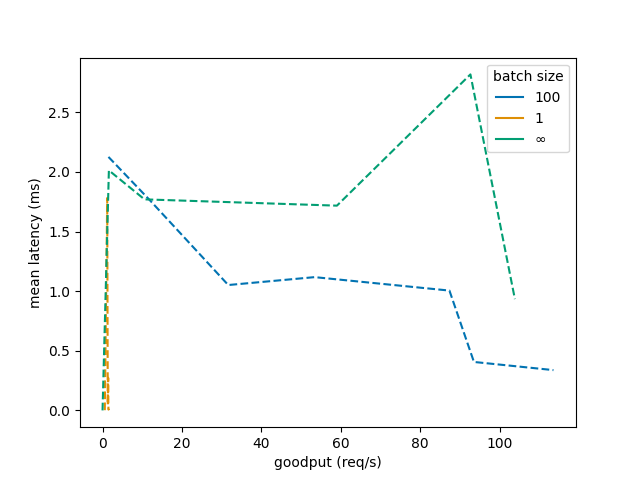
\includegraphics[scale=0.75]{mininet/throughputlatency.png}
\caption{Benchmarking of mean latency while varying throughputs and batch sizes, run for 10s with 100ms network delay.}
\end{figure}

\begin{figure}[h!]
\centering
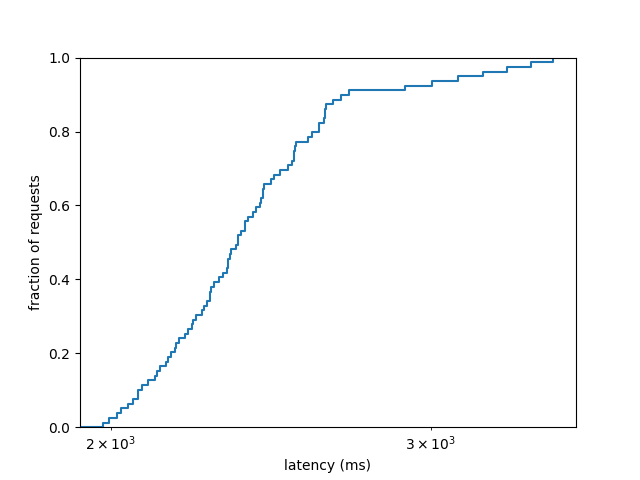
\includegraphics[scale=0.75]{mininet/10tpub_cumlatency.png}
\caption{Cumulative latency plot for experiment with a throughput of 10req/s and unlimited batch size, run for 10s with 100ms network delay.}
\end{figure}

[Give ablation graphs comparing the performance with 100ms delay, and without.]

\subsection{View-changes} \label{viewchangeeval}

\begin{figure}[h!]
\centering
\resizebox{\textwidth}{!}{%% Creator: Matplotlib, PGF backend
%%
%% To include the figure in your LaTeX document, write
%%   \input{<filename>.pgf}
%%
%% Make sure the required packages are loaded in your preamble
%%   \usepackage{pgf}
%%
%% Also ensure that all the required font packages are loaded; for instance,
%% the lmodern package is sometimes necessary when using math font.
%%   \usepackage{lmodern}
%%
%% Figures using additional raster images can only be included by \input if
%% they are in the same directory as the main LaTeX file. For loading figures
%% from other directories you can use the `import` package
%%   \usepackage{import}
%%
%% and then include the figures with
%%   \import{<path to file>}{<filename>.pgf}
%%
%% Matplotlib used the following preamble
%%   
%%   \usepackage{fontspec}
%%   \setmainfont{DejaVuSerif.ttf}[Path=\detokenize{/opt/homebrew/lib/python3.10/site-packages/matplotlib/mpl-data/fonts/ttf/}]
%%   \setsansfont{DejaVuSans.ttf}[Path=\detokenize{/opt/homebrew/lib/python3.10/site-packages/matplotlib/mpl-data/fonts/ttf/}]
%%   \setmonofont{DejaVuSansMono.ttf}[Path=\detokenize{/opt/homebrew/lib/python3.10/site-packages/matplotlib/mpl-data/fonts/ttf/}]
%%   \makeatletter\@ifpackageloaded{underscore}{}{\usepackage[strings]{underscore}}\makeatother
%%
\begingroup%
\makeatletter%
\begin{pgfpicture}%
\pgfpathrectangle{\pgfpointorigin}{\pgfqpoint{10.000000in}{5.000000in}}%
\pgfusepath{use as bounding box, clip}%
\begin{pgfscope}%
\pgfsetbuttcap%
\pgfsetmiterjoin%
\definecolor{currentfill}{rgb}{1.000000,1.000000,1.000000}%
\pgfsetfillcolor{currentfill}%
\pgfsetlinewidth{0.000000pt}%
\definecolor{currentstroke}{rgb}{1.000000,1.000000,1.000000}%
\pgfsetstrokecolor{currentstroke}%
\pgfsetdash{}{0pt}%
\pgfpathmoveto{\pgfqpoint{0.000000in}{0.000000in}}%
\pgfpathlineto{\pgfqpoint{10.000000in}{0.000000in}}%
\pgfpathlineto{\pgfqpoint{10.000000in}{5.000000in}}%
\pgfpathlineto{\pgfqpoint{0.000000in}{5.000000in}}%
\pgfpathlineto{\pgfqpoint{0.000000in}{0.000000in}}%
\pgfpathclose%
\pgfusepath{fill}%
\end{pgfscope}%
\begin{pgfscope}%
\pgfsetbuttcap%
\pgfsetmiterjoin%
\definecolor{currentfill}{rgb}{1.000000,1.000000,1.000000}%
\pgfsetfillcolor{currentfill}%
\pgfsetlinewidth{0.000000pt}%
\definecolor{currentstroke}{rgb}{0.000000,0.000000,0.000000}%
\pgfsetstrokecolor{currentstroke}%
\pgfsetstrokeopacity{0.000000}%
\pgfsetdash{}{0pt}%
\pgfpathmoveto{\pgfqpoint{0.549740in}{0.463273in}}%
\pgfpathlineto{\pgfqpoint{9.869965in}{0.463273in}}%
\pgfpathlineto{\pgfqpoint{9.869965in}{4.958330in}}%
\pgfpathlineto{\pgfqpoint{0.549740in}{4.958330in}}%
\pgfpathlineto{\pgfqpoint{0.549740in}{0.463273in}}%
\pgfpathclose%
\pgfusepath{fill}%
\end{pgfscope}%
\begin{pgfscope}%
\pgfpathrectangle{\pgfqpoint{0.549740in}{0.463273in}}{\pgfqpoint{9.320225in}{4.495057in}}%
\pgfusepath{clip}%
\pgfsetbuttcap%
\pgfsetroundjoin%
\pgfsetlinewidth{0.000000pt}%
\definecolor{currentstroke}{rgb}{0.000000,0.000000,0.000000}%
\pgfsetstrokecolor{currentstroke}%
\pgfsetdash{}{0pt}%
\pgfpathmoveto{\pgfqpoint{0.549761in}{0.667594in}}%
\pgfpathlineto{\pgfqpoint{0.735988in}{0.667594in}}%
\pgfpathlineto{\pgfqpoint{0.735988in}{0.749322in}}%
\pgfpathlineto{\pgfqpoint{0.549761in}{0.749322in}}%
\pgfpathlineto{\pgfqpoint{0.549761in}{0.667594in}}%
\pgfusepath{}%
\end{pgfscope}%
\begin{pgfscope}%
\pgfpathrectangle{\pgfqpoint{0.549740in}{0.463273in}}{\pgfqpoint{9.320225in}{4.495057in}}%
\pgfusepath{clip}%
\pgfsetbuttcap%
\pgfsetroundjoin%
\pgfsetlinewidth{0.000000pt}%
\definecolor{currentstroke}{rgb}{0.000000,0.000000,0.000000}%
\pgfsetstrokecolor{currentstroke}%
\pgfsetdash{}{0pt}%
\pgfpathmoveto{\pgfqpoint{0.735988in}{0.667594in}}%
\pgfpathlineto{\pgfqpoint{0.922214in}{0.667594in}}%
\pgfpathlineto{\pgfqpoint{0.922214in}{0.749322in}}%
\pgfpathlineto{\pgfqpoint{0.735988in}{0.749322in}}%
\pgfpathlineto{\pgfqpoint{0.735988in}{0.667594in}}%
\pgfusepath{}%
\end{pgfscope}%
\begin{pgfscope}%
\pgfpathrectangle{\pgfqpoint{0.549740in}{0.463273in}}{\pgfqpoint{9.320225in}{4.495057in}}%
\pgfusepath{clip}%
\pgfsetbuttcap%
\pgfsetroundjoin%
\pgfsetlinewidth{0.000000pt}%
\definecolor{currentstroke}{rgb}{0.000000,0.000000,0.000000}%
\pgfsetstrokecolor{currentstroke}%
\pgfsetdash{}{0pt}%
\pgfpathmoveto{\pgfqpoint{0.922214in}{0.667594in}}%
\pgfpathlineto{\pgfqpoint{1.108441in}{0.667594in}}%
\pgfpathlineto{\pgfqpoint{1.108441in}{0.749322in}}%
\pgfpathlineto{\pgfqpoint{0.922214in}{0.749322in}}%
\pgfpathlineto{\pgfqpoint{0.922214in}{0.667594in}}%
\pgfusepath{}%
\end{pgfscope}%
\begin{pgfscope}%
\pgfpathrectangle{\pgfqpoint{0.549740in}{0.463273in}}{\pgfqpoint{9.320225in}{4.495057in}}%
\pgfusepath{clip}%
\pgfsetbuttcap%
\pgfsetroundjoin%
\pgfsetlinewidth{0.000000pt}%
\definecolor{currentstroke}{rgb}{0.000000,0.000000,0.000000}%
\pgfsetstrokecolor{currentstroke}%
\pgfsetdash{}{0pt}%
\pgfpathmoveto{\pgfqpoint{1.108441in}{0.667594in}}%
\pgfpathlineto{\pgfqpoint{1.294667in}{0.667594in}}%
\pgfpathlineto{\pgfqpoint{1.294667in}{0.749322in}}%
\pgfpathlineto{\pgfqpoint{1.108441in}{0.749322in}}%
\pgfpathlineto{\pgfqpoint{1.108441in}{0.667594in}}%
\pgfusepath{}%
\end{pgfscope}%
\begin{pgfscope}%
\pgfpathrectangle{\pgfqpoint{0.549740in}{0.463273in}}{\pgfqpoint{9.320225in}{4.495057in}}%
\pgfusepath{clip}%
\pgfsetbuttcap%
\pgfsetroundjoin%
\pgfsetlinewidth{0.000000pt}%
\definecolor{currentstroke}{rgb}{0.000000,0.000000,0.000000}%
\pgfsetstrokecolor{currentstroke}%
\pgfsetdash{}{0pt}%
\pgfpathmoveto{\pgfqpoint{1.294667in}{0.667594in}}%
\pgfpathlineto{\pgfqpoint{1.480894in}{0.667594in}}%
\pgfpathlineto{\pgfqpoint{1.480894in}{0.749322in}}%
\pgfpathlineto{\pgfqpoint{1.294667in}{0.749322in}}%
\pgfpathlineto{\pgfqpoint{1.294667in}{0.667594in}}%
\pgfusepath{}%
\end{pgfscope}%
\begin{pgfscope}%
\pgfpathrectangle{\pgfqpoint{0.549740in}{0.463273in}}{\pgfqpoint{9.320225in}{4.495057in}}%
\pgfusepath{clip}%
\pgfsetbuttcap%
\pgfsetroundjoin%
\pgfsetlinewidth{0.000000pt}%
\definecolor{currentstroke}{rgb}{0.000000,0.000000,0.000000}%
\pgfsetstrokecolor{currentstroke}%
\pgfsetdash{}{0pt}%
\pgfpathmoveto{\pgfqpoint{1.480894in}{0.667594in}}%
\pgfpathlineto{\pgfqpoint{1.667120in}{0.667594in}}%
\pgfpathlineto{\pgfqpoint{1.667120in}{0.749322in}}%
\pgfpathlineto{\pgfqpoint{1.480894in}{0.749322in}}%
\pgfpathlineto{\pgfqpoint{1.480894in}{0.667594in}}%
\pgfusepath{}%
\end{pgfscope}%
\begin{pgfscope}%
\pgfpathrectangle{\pgfqpoint{0.549740in}{0.463273in}}{\pgfqpoint{9.320225in}{4.495057in}}%
\pgfusepath{clip}%
\pgfsetbuttcap%
\pgfsetroundjoin%
\pgfsetlinewidth{0.000000pt}%
\definecolor{currentstroke}{rgb}{0.000000,0.000000,0.000000}%
\pgfsetstrokecolor{currentstroke}%
\pgfsetdash{}{0pt}%
\pgfpathmoveto{\pgfqpoint{1.667120in}{0.667594in}}%
\pgfpathlineto{\pgfqpoint{1.853347in}{0.667594in}}%
\pgfpathlineto{\pgfqpoint{1.853347in}{0.749322in}}%
\pgfpathlineto{\pgfqpoint{1.667120in}{0.749322in}}%
\pgfpathlineto{\pgfqpoint{1.667120in}{0.667594in}}%
\pgfusepath{}%
\end{pgfscope}%
\begin{pgfscope}%
\pgfpathrectangle{\pgfqpoint{0.549740in}{0.463273in}}{\pgfqpoint{9.320225in}{4.495057in}}%
\pgfusepath{clip}%
\pgfsetbuttcap%
\pgfsetroundjoin%
\pgfsetlinewidth{0.000000pt}%
\definecolor{currentstroke}{rgb}{0.000000,0.000000,0.000000}%
\pgfsetstrokecolor{currentstroke}%
\pgfsetdash{}{0pt}%
\pgfpathmoveto{\pgfqpoint{1.853347in}{0.667594in}}%
\pgfpathlineto{\pgfqpoint{2.039573in}{0.667594in}}%
\pgfpathlineto{\pgfqpoint{2.039573in}{0.749322in}}%
\pgfpathlineto{\pgfqpoint{1.853347in}{0.749322in}}%
\pgfpathlineto{\pgfqpoint{1.853347in}{0.667594in}}%
\pgfusepath{}%
\end{pgfscope}%
\begin{pgfscope}%
\pgfpathrectangle{\pgfqpoint{0.549740in}{0.463273in}}{\pgfqpoint{9.320225in}{4.495057in}}%
\pgfusepath{clip}%
\pgfsetbuttcap%
\pgfsetroundjoin%
\pgfsetlinewidth{0.000000pt}%
\definecolor{currentstroke}{rgb}{0.000000,0.000000,0.000000}%
\pgfsetstrokecolor{currentstroke}%
\pgfsetdash{}{0pt}%
\pgfpathmoveto{\pgfqpoint{2.039573in}{0.667594in}}%
\pgfpathlineto{\pgfqpoint{2.225800in}{0.667594in}}%
\pgfpathlineto{\pgfqpoint{2.225800in}{0.749322in}}%
\pgfpathlineto{\pgfqpoint{2.039573in}{0.749322in}}%
\pgfpathlineto{\pgfqpoint{2.039573in}{0.667594in}}%
\pgfusepath{}%
\end{pgfscope}%
\begin{pgfscope}%
\pgfpathrectangle{\pgfqpoint{0.549740in}{0.463273in}}{\pgfqpoint{9.320225in}{4.495057in}}%
\pgfusepath{clip}%
\pgfsetbuttcap%
\pgfsetroundjoin%
\definecolor{currentfill}{rgb}{0.472869,0.711325,0.955316}%
\pgfsetfillcolor{currentfill}%
\pgfsetlinewidth{0.000000pt}%
\definecolor{currentstroke}{rgb}{0.000000,0.000000,0.000000}%
\pgfsetstrokecolor{currentstroke}%
\pgfsetdash{}{0pt}%
\pgfpathmoveto{\pgfqpoint{2.225800in}{0.667594in}}%
\pgfpathlineto{\pgfqpoint{2.412027in}{0.667594in}}%
\pgfpathlineto{\pgfqpoint{2.412027in}{0.749322in}}%
\pgfpathlineto{\pgfqpoint{2.225800in}{0.749322in}}%
\pgfpathlineto{\pgfqpoint{2.225800in}{0.667594in}}%
\pgfusepath{fill}%
\end{pgfscope}%
\begin{pgfscope}%
\pgfpathrectangle{\pgfqpoint{0.549740in}{0.463273in}}{\pgfqpoint{9.320225in}{4.495057in}}%
\pgfusepath{clip}%
\pgfsetbuttcap%
\pgfsetroundjoin%
\definecolor{currentfill}{rgb}{0.547810,0.736432,0.947518}%
\pgfsetfillcolor{currentfill}%
\pgfsetlinewidth{0.000000pt}%
\definecolor{currentstroke}{rgb}{0.000000,0.000000,0.000000}%
\pgfsetstrokecolor{currentstroke}%
\pgfsetdash{}{0pt}%
\pgfpathmoveto{\pgfqpoint{2.412027in}{0.667594in}}%
\pgfpathlineto{\pgfqpoint{2.598253in}{0.667594in}}%
\pgfpathlineto{\pgfqpoint{2.598253in}{0.749322in}}%
\pgfpathlineto{\pgfqpoint{2.412027in}{0.749322in}}%
\pgfpathlineto{\pgfqpoint{2.412027in}{0.667594in}}%
\pgfusepath{fill}%
\end{pgfscope}%
\begin{pgfscope}%
\pgfpathrectangle{\pgfqpoint{0.549740in}{0.463273in}}{\pgfqpoint{9.320225in}{4.495057in}}%
\pgfusepath{clip}%
\pgfsetbuttcap%
\pgfsetroundjoin%
\definecolor{currentfill}{rgb}{0.547810,0.736432,0.947518}%
\pgfsetfillcolor{currentfill}%
\pgfsetlinewidth{0.000000pt}%
\definecolor{currentstroke}{rgb}{0.000000,0.000000,0.000000}%
\pgfsetstrokecolor{currentstroke}%
\pgfsetdash{}{0pt}%
\pgfpathmoveto{\pgfqpoint{2.598253in}{0.667594in}}%
\pgfpathlineto{\pgfqpoint{2.784480in}{0.667594in}}%
\pgfpathlineto{\pgfqpoint{2.784480in}{0.749322in}}%
\pgfpathlineto{\pgfqpoint{2.598253in}{0.749322in}}%
\pgfpathlineto{\pgfqpoint{2.598253in}{0.667594in}}%
\pgfusepath{fill}%
\end{pgfscope}%
\begin{pgfscope}%
\pgfpathrectangle{\pgfqpoint{0.549740in}{0.463273in}}{\pgfqpoint{9.320225in}{4.495057in}}%
\pgfusepath{clip}%
\pgfsetbuttcap%
\pgfsetroundjoin%
\definecolor{currentfill}{rgb}{0.547810,0.736432,0.947518}%
\pgfsetfillcolor{currentfill}%
\pgfsetlinewidth{0.000000pt}%
\definecolor{currentstroke}{rgb}{0.000000,0.000000,0.000000}%
\pgfsetstrokecolor{currentstroke}%
\pgfsetdash{}{0pt}%
\pgfpathmoveto{\pgfqpoint{2.784480in}{0.667594in}}%
\pgfpathlineto{\pgfqpoint{2.970706in}{0.667594in}}%
\pgfpathlineto{\pgfqpoint{2.970706in}{0.749322in}}%
\pgfpathlineto{\pgfqpoint{2.784480in}{0.749322in}}%
\pgfpathlineto{\pgfqpoint{2.784480in}{0.667594in}}%
\pgfusepath{fill}%
\end{pgfscope}%
\begin{pgfscope}%
\pgfpathrectangle{\pgfqpoint{0.549740in}{0.463273in}}{\pgfqpoint{9.320225in}{4.495057in}}%
\pgfusepath{clip}%
\pgfsetbuttcap%
\pgfsetroundjoin%
\definecolor{currentfill}{rgb}{0.472869,0.711325,0.955316}%
\pgfsetfillcolor{currentfill}%
\pgfsetlinewidth{0.000000pt}%
\definecolor{currentstroke}{rgb}{0.000000,0.000000,0.000000}%
\pgfsetstrokecolor{currentstroke}%
\pgfsetdash{}{0pt}%
\pgfpathmoveto{\pgfqpoint{2.970706in}{0.667594in}}%
\pgfpathlineto{\pgfqpoint{3.156933in}{0.667594in}}%
\pgfpathlineto{\pgfqpoint{3.156933in}{0.749322in}}%
\pgfpathlineto{\pgfqpoint{2.970706in}{0.749322in}}%
\pgfpathlineto{\pgfqpoint{2.970706in}{0.667594in}}%
\pgfusepath{fill}%
\end{pgfscope}%
\begin{pgfscope}%
\pgfpathrectangle{\pgfqpoint{0.549740in}{0.463273in}}{\pgfqpoint{9.320225in}{4.495057in}}%
\pgfusepath{clip}%
\pgfsetbuttcap%
\pgfsetroundjoin%
\definecolor{currentfill}{rgb}{0.273225,0.662144,0.968515}%
\pgfsetfillcolor{currentfill}%
\pgfsetlinewidth{0.000000pt}%
\definecolor{currentstroke}{rgb}{0.000000,0.000000,0.000000}%
\pgfsetstrokecolor{currentstroke}%
\pgfsetdash{}{0pt}%
\pgfpathmoveto{\pgfqpoint{3.156933in}{0.667594in}}%
\pgfpathlineto{\pgfqpoint{3.343159in}{0.667594in}}%
\pgfpathlineto{\pgfqpoint{3.343159in}{0.749322in}}%
\pgfpathlineto{\pgfqpoint{3.156933in}{0.749322in}}%
\pgfpathlineto{\pgfqpoint{3.156933in}{0.667594in}}%
\pgfusepath{fill}%
\end{pgfscope}%
\begin{pgfscope}%
\pgfpathrectangle{\pgfqpoint{0.549740in}{0.463273in}}{\pgfqpoint{9.320225in}{4.495057in}}%
\pgfusepath{clip}%
\pgfsetbuttcap%
\pgfsetroundjoin%
\definecolor{currentfill}{rgb}{0.547810,0.736432,0.947518}%
\pgfsetfillcolor{currentfill}%
\pgfsetlinewidth{0.000000pt}%
\definecolor{currentstroke}{rgb}{0.000000,0.000000,0.000000}%
\pgfsetstrokecolor{currentstroke}%
\pgfsetdash{}{0pt}%
\pgfpathmoveto{\pgfqpoint{3.343159in}{0.667594in}}%
\pgfpathlineto{\pgfqpoint{3.529386in}{0.667594in}}%
\pgfpathlineto{\pgfqpoint{3.529386in}{0.749322in}}%
\pgfpathlineto{\pgfqpoint{3.343159in}{0.749322in}}%
\pgfpathlineto{\pgfqpoint{3.343159in}{0.667594in}}%
\pgfusepath{fill}%
\end{pgfscope}%
\begin{pgfscope}%
\pgfpathrectangle{\pgfqpoint{0.549740in}{0.463273in}}{\pgfqpoint{9.320225in}{4.495057in}}%
\pgfusepath{clip}%
\pgfsetbuttcap%
\pgfsetroundjoin%
\definecolor{currentfill}{rgb}{0.385185,0.686583,0.962589}%
\pgfsetfillcolor{currentfill}%
\pgfsetlinewidth{0.000000pt}%
\definecolor{currentstroke}{rgb}{0.000000,0.000000,0.000000}%
\pgfsetstrokecolor{currentstroke}%
\pgfsetdash{}{0pt}%
\pgfpathmoveto{\pgfqpoint{3.529386in}{0.667594in}}%
\pgfpathlineto{\pgfqpoint{3.715612in}{0.667594in}}%
\pgfpathlineto{\pgfqpoint{3.715612in}{0.749322in}}%
\pgfpathlineto{\pgfqpoint{3.529386in}{0.749322in}}%
\pgfpathlineto{\pgfqpoint{3.529386in}{0.667594in}}%
\pgfusepath{fill}%
\end{pgfscope}%
\begin{pgfscope}%
\pgfpathrectangle{\pgfqpoint{0.549740in}{0.463273in}}{\pgfqpoint{9.320225in}{4.495057in}}%
\pgfusepath{clip}%
\pgfsetbuttcap%
\pgfsetroundjoin%
\definecolor{currentfill}{rgb}{0.189527,0.635753,0.950228}%
\pgfsetfillcolor{currentfill}%
\pgfsetlinewidth{0.000000pt}%
\definecolor{currentstroke}{rgb}{0.000000,0.000000,0.000000}%
\pgfsetstrokecolor{currentstroke}%
\pgfsetdash{}{0pt}%
\pgfpathmoveto{\pgfqpoint{3.715612in}{0.667594in}}%
\pgfpathlineto{\pgfqpoint{3.901839in}{0.667594in}}%
\pgfpathlineto{\pgfqpoint{3.901839in}{0.749322in}}%
\pgfpathlineto{\pgfqpoint{3.715612in}{0.749322in}}%
\pgfpathlineto{\pgfqpoint{3.715612in}{0.667594in}}%
\pgfusepath{fill}%
\end{pgfscope}%
\begin{pgfscope}%
\pgfpathrectangle{\pgfqpoint{0.549740in}{0.463273in}}{\pgfqpoint{9.320225in}{4.495057in}}%
\pgfusepath{clip}%
\pgfsetbuttcap%
\pgfsetroundjoin%
\definecolor{currentfill}{rgb}{0.169712,0.607583,0.911334}%
\pgfsetfillcolor{currentfill}%
\pgfsetlinewidth{0.000000pt}%
\definecolor{currentstroke}{rgb}{0.000000,0.000000,0.000000}%
\pgfsetstrokecolor{currentstroke}%
\pgfsetdash{}{0pt}%
\pgfpathmoveto{\pgfqpoint{3.901839in}{0.667594in}}%
\pgfpathlineto{\pgfqpoint{4.088065in}{0.667594in}}%
\pgfpathlineto{\pgfqpoint{4.088065in}{0.749322in}}%
\pgfpathlineto{\pgfqpoint{3.901839in}{0.749322in}}%
\pgfpathlineto{\pgfqpoint{3.901839in}{0.667594in}}%
\pgfusepath{fill}%
\end{pgfscope}%
\begin{pgfscope}%
\pgfpathrectangle{\pgfqpoint{0.549740in}{0.463273in}}{\pgfqpoint{9.320225in}{4.495057in}}%
\pgfusepath{clip}%
\pgfsetbuttcap%
\pgfsetroundjoin%
\definecolor{currentfill}{rgb}{0.385185,0.686583,0.962589}%
\pgfsetfillcolor{currentfill}%
\pgfsetlinewidth{0.000000pt}%
\definecolor{currentstroke}{rgb}{0.000000,0.000000,0.000000}%
\pgfsetstrokecolor{currentstroke}%
\pgfsetdash{}{0pt}%
\pgfpathmoveto{\pgfqpoint{4.088065in}{0.667594in}}%
\pgfpathlineto{\pgfqpoint{4.274292in}{0.667594in}}%
\pgfpathlineto{\pgfqpoint{4.274292in}{0.749322in}}%
\pgfpathlineto{\pgfqpoint{4.088065in}{0.749322in}}%
\pgfpathlineto{\pgfqpoint{4.088065in}{0.667594in}}%
\pgfusepath{fill}%
\end{pgfscope}%
\begin{pgfscope}%
\pgfpathrectangle{\pgfqpoint{0.549740in}{0.463273in}}{\pgfqpoint{9.320225in}{4.495057in}}%
\pgfusepath{clip}%
\pgfsetbuttcap%
\pgfsetroundjoin%
\definecolor{currentfill}{rgb}{0.169712,0.607583,0.911334}%
\pgfsetfillcolor{currentfill}%
\pgfsetlinewidth{0.000000pt}%
\definecolor{currentstroke}{rgb}{0.000000,0.000000,0.000000}%
\pgfsetstrokecolor{currentstroke}%
\pgfsetdash{}{0pt}%
\pgfpathmoveto{\pgfqpoint{4.274292in}{0.667594in}}%
\pgfpathlineto{\pgfqpoint{4.460519in}{0.667594in}}%
\pgfpathlineto{\pgfqpoint{4.460519in}{0.749322in}}%
\pgfpathlineto{\pgfqpoint{4.274292in}{0.749322in}}%
\pgfpathlineto{\pgfqpoint{4.274292in}{0.667594in}}%
\pgfusepath{fill}%
\end{pgfscope}%
\begin{pgfscope}%
\pgfpathrectangle{\pgfqpoint{0.549740in}{0.463273in}}{\pgfqpoint{9.320225in}{4.495057in}}%
\pgfusepath{clip}%
\pgfsetbuttcap%
\pgfsetroundjoin%
\definecolor{currentfill}{rgb}{0.163625,0.579322,0.869386}%
\pgfsetfillcolor{currentfill}%
\pgfsetlinewidth{0.000000pt}%
\definecolor{currentstroke}{rgb}{0.000000,0.000000,0.000000}%
\pgfsetstrokecolor{currentstroke}%
\pgfsetdash{}{0pt}%
\pgfpathmoveto{\pgfqpoint{4.460519in}{0.667594in}}%
\pgfpathlineto{\pgfqpoint{4.646745in}{0.667594in}}%
\pgfpathlineto{\pgfqpoint{4.646745in}{0.749322in}}%
\pgfpathlineto{\pgfqpoint{4.460519in}{0.749322in}}%
\pgfpathlineto{\pgfqpoint{4.460519in}{0.667594in}}%
\pgfusepath{fill}%
\end{pgfscope}%
\begin{pgfscope}%
\pgfpathrectangle{\pgfqpoint{0.549740in}{0.463273in}}{\pgfqpoint{9.320225in}{4.495057in}}%
\pgfusepath{clip}%
\pgfsetbuttcap%
\pgfsetroundjoin%
\definecolor{currentfill}{rgb}{0.273225,0.662144,0.968515}%
\pgfsetfillcolor{currentfill}%
\pgfsetlinewidth{0.000000pt}%
\definecolor{currentstroke}{rgb}{0.000000,0.000000,0.000000}%
\pgfsetstrokecolor{currentstroke}%
\pgfsetdash{}{0pt}%
\pgfpathmoveto{\pgfqpoint{4.646745in}{0.667594in}}%
\pgfpathlineto{\pgfqpoint{4.832972in}{0.667594in}}%
\pgfpathlineto{\pgfqpoint{4.832972in}{0.749322in}}%
\pgfpathlineto{\pgfqpoint{4.646745in}{0.749322in}}%
\pgfpathlineto{\pgfqpoint{4.646745in}{0.667594in}}%
\pgfusepath{fill}%
\end{pgfscope}%
\begin{pgfscope}%
\pgfpathrectangle{\pgfqpoint{0.549740in}{0.463273in}}{\pgfqpoint{9.320225in}{4.495057in}}%
\pgfusepath{clip}%
\pgfsetbuttcap%
\pgfsetroundjoin%
\definecolor{currentfill}{rgb}{0.189527,0.635753,0.950228}%
\pgfsetfillcolor{currentfill}%
\pgfsetlinewidth{0.000000pt}%
\definecolor{currentstroke}{rgb}{0.000000,0.000000,0.000000}%
\pgfsetstrokecolor{currentstroke}%
\pgfsetdash{}{0pt}%
\pgfpathmoveto{\pgfqpoint{4.832972in}{0.667594in}}%
\pgfpathlineto{\pgfqpoint{5.019198in}{0.667594in}}%
\pgfpathlineto{\pgfqpoint{5.019198in}{0.749322in}}%
\pgfpathlineto{\pgfqpoint{4.832972in}{0.749322in}}%
\pgfpathlineto{\pgfqpoint{4.832972in}{0.667594in}}%
\pgfusepath{fill}%
\end{pgfscope}%
\begin{pgfscope}%
\pgfpathrectangle{\pgfqpoint{0.549740in}{0.463273in}}{\pgfqpoint{9.320225in}{4.495057in}}%
\pgfusepath{clip}%
\pgfsetbuttcap%
\pgfsetroundjoin%
\pgfsetlinewidth{0.000000pt}%
\definecolor{currentstroke}{rgb}{0.000000,0.000000,0.000000}%
\pgfsetstrokecolor{currentstroke}%
\pgfsetdash{}{0pt}%
\pgfpathmoveto{\pgfqpoint{5.019198in}{0.667594in}}%
\pgfpathlineto{\pgfqpoint{5.205425in}{0.667594in}}%
\pgfpathlineto{\pgfqpoint{5.205425in}{0.749322in}}%
\pgfpathlineto{\pgfqpoint{5.019198in}{0.749322in}}%
\pgfpathlineto{\pgfqpoint{5.019198in}{0.667594in}}%
\pgfusepath{}%
\end{pgfscope}%
\begin{pgfscope}%
\pgfpathrectangle{\pgfqpoint{0.549740in}{0.463273in}}{\pgfqpoint{9.320225in}{4.495057in}}%
\pgfusepath{clip}%
\pgfsetbuttcap%
\pgfsetroundjoin%
\pgfsetlinewidth{0.000000pt}%
\definecolor{currentstroke}{rgb}{0.000000,0.000000,0.000000}%
\pgfsetstrokecolor{currentstroke}%
\pgfsetdash{}{0pt}%
\pgfpathmoveto{\pgfqpoint{5.205425in}{0.667594in}}%
\pgfpathlineto{\pgfqpoint{5.391651in}{0.667594in}}%
\pgfpathlineto{\pgfqpoint{5.391651in}{0.749322in}}%
\pgfpathlineto{\pgfqpoint{5.205425in}{0.749322in}}%
\pgfpathlineto{\pgfqpoint{5.205425in}{0.667594in}}%
\pgfusepath{}%
\end{pgfscope}%
\begin{pgfscope}%
\pgfpathrectangle{\pgfqpoint{0.549740in}{0.463273in}}{\pgfqpoint{9.320225in}{4.495057in}}%
\pgfusepath{clip}%
\pgfsetbuttcap%
\pgfsetroundjoin%
\pgfsetlinewidth{0.000000pt}%
\definecolor{currentstroke}{rgb}{0.000000,0.000000,0.000000}%
\pgfsetstrokecolor{currentstroke}%
\pgfsetdash{}{0pt}%
\pgfpathmoveto{\pgfqpoint{5.391651in}{0.667594in}}%
\pgfpathlineto{\pgfqpoint{5.577878in}{0.667594in}}%
\pgfpathlineto{\pgfqpoint{5.577878in}{0.749322in}}%
\pgfpathlineto{\pgfqpoint{5.391651in}{0.749322in}}%
\pgfpathlineto{\pgfqpoint{5.391651in}{0.667594in}}%
\pgfusepath{}%
\end{pgfscope}%
\begin{pgfscope}%
\pgfpathrectangle{\pgfqpoint{0.549740in}{0.463273in}}{\pgfqpoint{9.320225in}{4.495057in}}%
\pgfusepath{clip}%
\pgfsetbuttcap%
\pgfsetroundjoin%
\pgfsetlinewidth{0.000000pt}%
\definecolor{currentstroke}{rgb}{0.000000,0.000000,0.000000}%
\pgfsetstrokecolor{currentstroke}%
\pgfsetdash{}{0pt}%
\pgfpathmoveto{\pgfqpoint{5.577878in}{0.667594in}}%
\pgfpathlineto{\pgfqpoint{5.764104in}{0.667594in}}%
\pgfpathlineto{\pgfqpoint{5.764104in}{0.749322in}}%
\pgfpathlineto{\pgfqpoint{5.577878in}{0.749322in}}%
\pgfpathlineto{\pgfqpoint{5.577878in}{0.667594in}}%
\pgfusepath{}%
\end{pgfscope}%
\begin{pgfscope}%
\pgfpathrectangle{\pgfqpoint{0.549740in}{0.463273in}}{\pgfqpoint{9.320225in}{4.495057in}}%
\pgfusepath{clip}%
\pgfsetbuttcap%
\pgfsetroundjoin%
\pgfsetlinewidth{0.000000pt}%
\definecolor{currentstroke}{rgb}{0.000000,0.000000,0.000000}%
\pgfsetstrokecolor{currentstroke}%
\pgfsetdash{}{0pt}%
\pgfpathmoveto{\pgfqpoint{5.764104in}{0.667594in}}%
\pgfpathlineto{\pgfqpoint{5.950331in}{0.667594in}}%
\pgfpathlineto{\pgfqpoint{5.950331in}{0.749322in}}%
\pgfpathlineto{\pgfqpoint{5.764104in}{0.749322in}}%
\pgfpathlineto{\pgfqpoint{5.764104in}{0.667594in}}%
\pgfusepath{}%
\end{pgfscope}%
\begin{pgfscope}%
\pgfpathrectangle{\pgfqpoint{0.549740in}{0.463273in}}{\pgfqpoint{9.320225in}{4.495057in}}%
\pgfusepath{clip}%
\pgfsetbuttcap%
\pgfsetroundjoin%
\pgfsetlinewidth{0.000000pt}%
\definecolor{currentstroke}{rgb}{0.000000,0.000000,0.000000}%
\pgfsetstrokecolor{currentstroke}%
\pgfsetdash{}{0pt}%
\pgfpathmoveto{\pgfqpoint{5.950331in}{0.667594in}}%
\pgfpathlineto{\pgfqpoint{6.136557in}{0.667594in}}%
\pgfpathlineto{\pgfqpoint{6.136557in}{0.749322in}}%
\pgfpathlineto{\pgfqpoint{5.950331in}{0.749322in}}%
\pgfpathlineto{\pgfqpoint{5.950331in}{0.667594in}}%
\pgfusepath{}%
\end{pgfscope}%
\begin{pgfscope}%
\pgfpathrectangle{\pgfqpoint{0.549740in}{0.463273in}}{\pgfqpoint{9.320225in}{4.495057in}}%
\pgfusepath{clip}%
\pgfsetbuttcap%
\pgfsetroundjoin%
\pgfsetlinewidth{0.000000pt}%
\definecolor{currentstroke}{rgb}{0.000000,0.000000,0.000000}%
\pgfsetstrokecolor{currentstroke}%
\pgfsetdash{}{0pt}%
\pgfpathmoveto{\pgfqpoint{6.136557in}{0.667594in}}%
\pgfpathlineto{\pgfqpoint{6.322784in}{0.667594in}}%
\pgfpathlineto{\pgfqpoint{6.322784in}{0.749322in}}%
\pgfpathlineto{\pgfqpoint{6.136557in}{0.749322in}}%
\pgfpathlineto{\pgfqpoint{6.136557in}{0.667594in}}%
\pgfusepath{}%
\end{pgfscope}%
\begin{pgfscope}%
\pgfpathrectangle{\pgfqpoint{0.549740in}{0.463273in}}{\pgfqpoint{9.320225in}{4.495057in}}%
\pgfusepath{clip}%
\pgfsetbuttcap%
\pgfsetroundjoin%
\pgfsetlinewidth{0.000000pt}%
\definecolor{currentstroke}{rgb}{0.000000,0.000000,0.000000}%
\pgfsetstrokecolor{currentstroke}%
\pgfsetdash{}{0pt}%
\pgfpathmoveto{\pgfqpoint{6.322784in}{0.667594in}}%
\pgfpathlineto{\pgfqpoint{6.509011in}{0.667594in}}%
\pgfpathlineto{\pgfqpoint{6.509011in}{0.749322in}}%
\pgfpathlineto{\pgfqpoint{6.322784in}{0.749322in}}%
\pgfpathlineto{\pgfqpoint{6.322784in}{0.667594in}}%
\pgfusepath{}%
\end{pgfscope}%
\begin{pgfscope}%
\pgfpathrectangle{\pgfqpoint{0.549740in}{0.463273in}}{\pgfqpoint{9.320225in}{4.495057in}}%
\pgfusepath{clip}%
\pgfsetbuttcap%
\pgfsetroundjoin%
\pgfsetlinewidth{0.000000pt}%
\definecolor{currentstroke}{rgb}{0.000000,0.000000,0.000000}%
\pgfsetstrokecolor{currentstroke}%
\pgfsetdash{}{0pt}%
\pgfpathmoveto{\pgfqpoint{6.509011in}{0.667594in}}%
\pgfpathlineto{\pgfqpoint{6.695237in}{0.667594in}}%
\pgfpathlineto{\pgfqpoint{6.695237in}{0.749322in}}%
\pgfpathlineto{\pgfqpoint{6.509011in}{0.749322in}}%
\pgfpathlineto{\pgfqpoint{6.509011in}{0.667594in}}%
\pgfusepath{}%
\end{pgfscope}%
\begin{pgfscope}%
\pgfpathrectangle{\pgfqpoint{0.549740in}{0.463273in}}{\pgfqpoint{9.320225in}{4.495057in}}%
\pgfusepath{clip}%
\pgfsetbuttcap%
\pgfsetroundjoin%
\pgfsetlinewidth{0.000000pt}%
\definecolor{currentstroke}{rgb}{0.000000,0.000000,0.000000}%
\pgfsetstrokecolor{currentstroke}%
\pgfsetdash{}{0pt}%
\pgfpathmoveto{\pgfqpoint{6.695237in}{0.667594in}}%
\pgfpathlineto{\pgfqpoint{6.881464in}{0.667594in}}%
\pgfpathlineto{\pgfqpoint{6.881464in}{0.749322in}}%
\pgfpathlineto{\pgfqpoint{6.695237in}{0.749322in}}%
\pgfpathlineto{\pgfqpoint{6.695237in}{0.667594in}}%
\pgfusepath{}%
\end{pgfscope}%
\begin{pgfscope}%
\pgfpathrectangle{\pgfqpoint{0.549740in}{0.463273in}}{\pgfqpoint{9.320225in}{4.495057in}}%
\pgfusepath{clip}%
\pgfsetbuttcap%
\pgfsetroundjoin%
\pgfsetlinewidth{0.000000pt}%
\definecolor{currentstroke}{rgb}{0.000000,0.000000,0.000000}%
\pgfsetstrokecolor{currentstroke}%
\pgfsetdash{}{0pt}%
\pgfpathmoveto{\pgfqpoint{6.881464in}{0.667594in}}%
\pgfpathlineto{\pgfqpoint{7.067690in}{0.667594in}}%
\pgfpathlineto{\pgfqpoint{7.067690in}{0.749322in}}%
\pgfpathlineto{\pgfqpoint{6.881464in}{0.749322in}}%
\pgfpathlineto{\pgfqpoint{6.881464in}{0.667594in}}%
\pgfusepath{}%
\end{pgfscope}%
\begin{pgfscope}%
\pgfpathrectangle{\pgfqpoint{0.549740in}{0.463273in}}{\pgfqpoint{9.320225in}{4.495057in}}%
\pgfusepath{clip}%
\pgfsetbuttcap%
\pgfsetroundjoin%
\pgfsetlinewidth{0.000000pt}%
\definecolor{currentstroke}{rgb}{0.000000,0.000000,0.000000}%
\pgfsetstrokecolor{currentstroke}%
\pgfsetdash{}{0pt}%
\pgfpathmoveto{\pgfqpoint{7.067690in}{0.667594in}}%
\pgfpathlineto{\pgfqpoint{7.253917in}{0.667594in}}%
\pgfpathlineto{\pgfqpoint{7.253917in}{0.749322in}}%
\pgfpathlineto{\pgfqpoint{7.067690in}{0.749322in}}%
\pgfpathlineto{\pgfqpoint{7.067690in}{0.667594in}}%
\pgfusepath{}%
\end{pgfscope}%
\begin{pgfscope}%
\pgfpathrectangle{\pgfqpoint{0.549740in}{0.463273in}}{\pgfqpoint{9.320225in}{4.495057in}}%
\pgfusepath{clip}%
\pgfsetbuttcap%
\pgfsetroundjoin%
\pgfsetlinewidth{0.000000pt}%
\definecolor{currentstroke}{rgb}{0.000000,0.000000,0.000000}%
\pgfsetstrokecolor{currentstroke}%
\pgfsetdash{}{0pt}%
\pgfpathmoveto{\pgfqpoint{7.253917in}{0.667594in}}%
\pgfpathlineto{\pgfqpoint{7.440143in}{0.667594in}}%
\pgfpathlineto{\pgfqpoint{7.440143in}{0.749322in}}%
\pgfpathlineto{\pgfqpoint{7.253917in}{0.749322in}}%
\pgfpathlineto{\pgfqpoint{7.253917in}{0.667594in}}%
\pgfusepath{}%
\end{pgfscope}%
\begin{pgfscope}%
\pgfpathrectangle{\pgfqpoint{0.549740in}{0.463273in}}{\pgfqpoint{9.320225in}{4.495057in}}%
\pgfusepath{clip}%
\pgfsetbuttcap%
\pgfsetroundjoin%
\pgfsetlinewidth{0.000000pt}%
\definecolor{currentstroke}{rgb}{0.000000,0.000000,0.000000}%
\pgfsetstrokecolor{currentstroke}%
\pgfsetdash{}{0pt}%
\pgfpathmoveto{\pgfqpoint{7.440143in}{0.667594in}}%
\pgfpathlineto{\pgfqpoint{7.626370in}{0.667594in}}%
\pgfpathlineto{\pgfqpoint{7.626370in}{0.749322in}}%
\pgfpathlineto{\pgfqpoint{7.440143in}{0.749322in}}%
\pgfpathlineto{\pgfqpoint{7.440143in}{0.667594in}}%
\pgfusepath{}%
\end{pgfscope}%
\begin{pgfscope}%
\pgfpathrectangle{\pgfqpoint{0.549740in}{0.463273in}}{\pgfqpoint{9.320225in}{4.495057in}}%
\pgfusepath{clip}%
\pgfsetbuttcap%
\pgfsetroundjoin%
\pgfsetlinewidth{0.000000pt}%
\definecolor{currentstroke}{rgb}{0.000000,0.000000,0.000000}%
\pgfsetstrokecolor{currentstroke}%
\pgfsetdash{}{0pt}%
\pgfpathmoveto{\pgfqpoint{7.626370in}{0.667594in}}%
\pgfpathlineto{\pgfqpoint{7.812596in}{0.667594in}}%
\pgfpathlineto{\pgfqpoint{7.812596in}{0.749322in}}%
\pgfpathlineto{\pgfqpoint{7.626370in}{0.749322in}}%
\pgfpathlineto{\pgfqpoint{7.626370in}{0.667594in}}%
\pgfusepath{}%
\end{pgfscope}%
\begin{pgfscope}%
\pgfpathrectangle{\pgfqpoint{0.549740in}{0.463273in}}{\pgfqpoint{9.320225in}{4.495057in}}%
\pgfusepath{clip}%
\pgfsetbuttcap%
\pgfsetroundjoin%
\pgfsetlinewidth{0.000000pt}%
\definecolor{currentstroke}{rgb}{0.000000,0.000000,0.000000}%
\pgfsetstrokecolor{currentstroke}%
\pgfsetdash{}{0pt}%
\pgfpathmoveto{\pgfqpoint{7.812596in}{0.667594in}}%
\pgfpathlineto{\pgfqpoint{7.998823in}{0.667594in}}%
\pgfpathlineto{\pgfqpoint{7.998823in}{0.749322in}}%
\pgfpathlineto{\pgfqpoint{7.812596in}{0.749322in}}%
\pgfpathlineto{\pgfqpoint{7.812596in}{0.667594in}}%
\pgfusepath{}%
\end{pgfscope}%
\begin{pgfscope}%
\pgfpathrectangle{\pgfqpoint{0.549740in}{0.463273in}}{\pgfqpoint{9.320225in}{4.495057in}}%
\pgfusepath{clip}%
\pgfsetbuttcap%
\pgfsetroundjoin%
\pgfsetlinewidth{0.000000pt}%
\definecolor{currentstroke}{rgb}{0.000000,0.000000,0.000000}%
\pgfsetstrokecolor{currentstroke}%
\pgfsetdash{}{0pt}%
\pgfpathmoveto{\pgfqpoint{7.998823in}{0.667594in}}%
\pgfpathlineto{\pgfqpoint{8.185049in}{0.667594in}}%
\pgfpathlineto{\pgfqpoint{8.185049in}{0.749322in}}%
\pgfpathlineto{\pgfqpoint{7.998823in}{0.749322in}}%
\pgfpathlineto{\pgfqpoint{7.998823in}{0.667594in}}%
\pgfusepath{}%
\end{pgfscope}%
\begin{pgfscope}%
\pgfpathrectangle{\pgfqpoint{0.549740in}{0.463273in}}{\pgfqpoint{9.320225in}{4.495057in}}%
\pgfusepath{clip}%
\pgfsetbuttcap%
\pgfsetroundjoin%
\pgfsetlinewidth{0.000000pt}%
\definecolor{currentstroke}{rgb}{0.000000,0.000000,0.000000}%
\pgfsetstrokecolor{currentstroke}%
\pgfsetdash{}{0pt}%
\pgfpathmoveto{\pgfqpoint{8.185049in}{0.667594in}}%
\pgfpathlineto{\pgfqpoint{8.371276in}{0.667594in}}%
\pgfpathlineto{\pgfqpoint{8.371276in}{0.749322in}}%
\pgfpathlineto{\pgfqpoint{8.185049in}{0.749322in}}%
\pgfpathlineto{\pgfqpoint{8.185049in}{0.667594in}}%
\pgfusepath{}%
\end{pgfscope}%
\begin{pgfscope}%
\pgfpathrectangle{\pgfqpoint{0.549740in}{0.463273in}}{\pgfqpoint{9.320225in}{4.495057in}}%
\pgfusepath{clip}%
\pgfsetbuttcap%
\pgfsetroundjoin%
\pgfsetlinewidth{0.000000pt}%
\definecolor{currentstroke}{rgb}{0.000000,0.000000,0.000000}%
\pgfsetstrokecolor{currentstroke}%
\pgfsetdash{}{0pt}%
\pgfpathmoveto{\pgfqpoint{8.371276in}{0.667594in}}%
\pgfpathlineto{\pgfqpoint{8.557503in}{0.667594in}}%
\pgfpathlineto{\pgfqpoint{8.557503in}{0.749322in}}%
\pgfpathlineto{\pgfqpoint{8.371276in}{0.749322in}}%
\pgfpathlineto{\pgfqpoint{8.371276in}{0.667594in}}%
\pgfusepath{}%
\end{pgfscope}%
\begin{pgfscope}%
\pgfpathrectangle{\pgfqpoint{0.549740in}{0.463273in}}{\pgfqpoint{9.320225in}{4.495057in}}%
\pgfusepath{clip}%
\pgfsetbuttcap%
\pgfsetroundjoin%
\pgfsetlinewidth{0.000000pt}%
\definecolor{currentstroke}{rgb}{0.000000,0.000000,0.000000}%
\pgfsetstrokecolor{currentstroke}%
\pgfsetdash{}{0pt}%
\pgfpathmoveto{\pgfqpoint{8.557503in}{0.667594in}}%
\pgfpathlineto{\pgfqpoint{8.743729in}{0.667594in}}%
\pgfpathlineto{\pgfqpoint{8.743729in}{0.749322in}}%
\pgfpathlineto{\pgfqpoint{8.557503in}{0.749322in}}%
\pgfpathlineto{\pgfqpoint{8.557503in}{0.667594in}}%
\pgfusepath{}%
\end{pgfscope}%
\begin{pgfscope}%
\pgfpathrectangle{\pgfqpoint{0.549740in}{0.463273in}}{\pgfqpoint{9.320225in}{4.495057in}}%
\pgfusepath{clip}%
\pgfsetbuttcap%
\pgfsetroundjoin%
\pgfsetlinewidth{0.000000pt}%
\definecolor{currentstroke}{rgb}{0.000000,0.000000,0.000000}%
\pgfsetstrokecolor{currentstroke}%
\pgfsetdash{}{0pt}%
\pgfpathmoveto{\pgfqpoint{8.743729in}{0.667594in}}%
\pgfpathlineto{\pgfqpoint{8.929956in}{0.667594in}}%
\pgfpathlineto{\pgfqpoint{8.929956in}{0.749322in}}%
\pgfpathlineto{\pgfqpoint{8.743729in}{0.749322in}}%
\pgfpathlineto{\pgfqpoint{8.743729in}{0.667594in}}%
\pgfusepath{}%
\end{pgfscope}%
\begin{pgfscope}%
\pgfpathrectangle{\pgfqpoint{0.549740in}{0.463273in}}{\pgfqpoint{9.320225in}{4.495057in}}%
\pgfusepath{clip}%
\pgfsetbuttcap%
\pgfsetroundjoin%
\pgfsetlinewidth{0.000000pt}%
\definecolor{currentstroke}{rgb}{0.000000,0.000000,0.000000}%
\pgfsetstrokecolor{currentstroke}%
\pgfsetdash{}{0pt}%
\pgfpathmoveto{\pgfqpoint{8.929956in}{0.667594in}}%
\pgfpathlineto{\pgfqpoint{9.116182in}{0.667594in}}%
\pgfpathlineto{\pgfqpoint{9.116182in}{0.749322in}}%
\pgfpathlineto{\pgfqpoint{8.929956in}{0.749322in}}%
\pgfpathlineto{\pgfqpoint{8.929956in}{0.667594in}}%
\pgfusepath{}%
\end{pgfscope}%
\begin{pgfscope}%
\pgfpathrectangle{\pgfqpoint{0.549740in}{0.463273in}}{\pgfqpoint{9.320225in}{4.495057in}}%
\pgfusepath{clip}%
\pgfsetbuttcap%
\pgfsetroundjoin%
\pgfsetlinewidth{0.000000pt}%
\definecolor{currentstroke}{rgb}{0.000000,0.000000,0.000000}%
\pgfsetstrokecolor{currentstroke}%
\pgfsetdash{}{0pt}%
\pgfpathmoveto{\pgfqpoint{9.116182in}{0.667594in}}%
\pgfpathlineto{\pgfqpoint{9.302409in}{0.667594in}}%
\pgfpathlineto{\pgfqpoint{9.302409in}{0.749322in}}%
\pgfpathlineto{\pgfqpoint{9.116182in}{0.749322in}}%
\pgfpathlineto{\pgfqpoint{9.116182in}{0.667594in}}%
\pgfusepath{}%
\end{pgfscope}%
\begin{pgfscope}%
\pgfpathrectangle{\pgfqpoint{0.549740in}{0.463273in}}{\pgfqpoint{9.320225in}{4.495057in}}%
\pgfusepath{clip}%
\pgfsetbuttcap%
\pgfsetroundjoin%
\pgfsetlinewidth{0.000000pt}%
\definecolor{currentstroke}{rgb}{0.000000,0.000000,0.000000}%
\pgfsetstrokecolor{currentstroke}%
\pgfsetdash{}{0pt}%
\pgfpathmoveto{\pgfqpoint{9.302409in}{0.667594in}}%
\pgfpathlineto{\pgfqpoint{9.488635in}{0.667594in}}%
\pgfpathlineto{\pgfqpoint{9.488635in}{0.749322in}}%
\pgfpathlineto{\pgfqpoint{9.302409in}{0.749322in}}%
\pgfpathlineto{\pgfqpoint{9.302409in}{0.667594in}}%
\pgfusepath{}%
\end{pgfscope}%
\begin{pgfscope}%
\pgfpathrectangle{\pgfqpoint{0.549740in}{0.463273in}}{\pgfqpoint{9.320225in}{4.495057in}}%
\pgfusepath{clip}%
\pgfsetbuttcap%
\pgfsetroundjoin%
\pgfsetlinewidth{0.000000pt}%
\definecolor{currentstroke}{rgb}{0.000000,0.000000,0.000000}%
\pgfsetstrokecolor{currentstroke}%
\pgfsetdash{}{0pt}%
\pgfpathmoveto{\pgfqpoint{9.488635in}{0.667594in}}%
\pgfpathlineto{\pgfqpoint{9.674862in}{0.667594in}}%
\pgfpathlineto{\pgfqpoint{9.674862in}{0.749322in}}%
\pgfpathlineto{\pgfqpoint{9.488635in}{0.749322in}}%
\pgfpathlineto{\pgfqpoint{9.488635in}{0.667594in}}%
\pgfusepath{}%
\end{pgfscope}%
\begin{pgfscope}%
\pgfpathrectangle{\pgfqpoint{0.549740in}{0.463273in}}{\pgfqpoint{9.320225in}{4.495057in}}%
\pgfusepath{clip}%
\pgfsetbuttcap%
\pgfsetroundjoin%
\pgfsetlinewidth{0.000000pt}%
\definecolor{currentstroke}{rgb}{0.000000,0.000000,0.000000}%
\pgfsetstrokecolor{currentstroke}%
\pgfsetdash{}{0pt}%
\pgfpathmoveto{\pgfqpoint{9.674862in}{0.667594in}}%
\pgfpathlineto{\pgfqpoint{9.861088in}{0.667594in}}%
\pgfpathlineto{\pgfqpoint{9.861088in}{0.749322in}}%
\pgfpathlineto{\pgfqpoint{9.674862in}{0.749322in}}%
\pgfpathlineto{\pgfqpoint{9.674862in}{0.667594in}}%
\pgfusepath{}%
\end{pgfscope}%
\begin{pgfscope}%
\pgfpathrectangle{\pgfqpoint{0.549740in}{0.463273in}}{\pgfqpoint{9.320225in}{4.495057in}}%
\pgfusepath{clip}%
\pgfsetbuttcap%
\pgfsetroundjoin%
\definecolor{currentfill}{rgb}{0.385185,0.686583,0.962589}%
\pgfsetfillcolor{currentfill}%
\pgfsetlinewidth{0.000000pt}%
\definecolor{currentstroke}{rgb}{0.000000,0.000000,0.000000}%
\pgfsetstrokecolor{currentstroke}%
\pgfsetdash{}{0pt}%
\pgfpathmoveto{\pgfqpoint{0.549761in}{0.749322in}}%
\pgfpathlineto{\pgfqpoint{0.735988in}{0.749322in}}%
\pgfpathlineto{\pgfqpoint{0.735988in}{0.831051in}}%
\pgfpathlineto{\pgfqpoint{0.549761in}{0.831051in}}%
\pgfpathlineto{\pgfqpoint{0.549761in}{0.749322in}}%
\pgfusepath{fill}%
\end{pgfscope}%
\begin{pgfscope}%
\pgfpathrectangle{\pgfqpoint{0.549740in}{0.463273in}}{\pgfqpoint{9.320225in}{4.495057in}}%
\pgfusepath{clip}%
\pgfsetbuttcap%
\pgfsetroundjoin%
\definecolor{currentfill}{rgb}{0.614330,0.761948,0.940009}%
\pgfsetfillcolor{currentfill}%
\pgfsetlinewidth{0.000000pt}%
\definecolor{currentstroke}{rgb}{0.000000,0.000000,0.000000}%
\pgfsetstrokecolor{currentstroke}%
\pgfsetdash{}{0pt}%
\pgfpathmoveto{\pgfqpoint{0.735988in}{0.749322in}}%
\pgfpathlineto{\pgfqpoint{0.922214in}{0.749322in}}%
\pgfpathlineto{\pgfqpoint{0.922214in}{0.831051in}}%
\pgfpathlineto{\pgfqpoint{0.735988in}{0.831051in}}%
\pgfpathlineto{\pgfqpoint{0.735988in}{0.749322in}}%
\pgfusepath{fill}%
\end{pgfscope}%
\begin{pgfscope}%
\pgfpathrectangle{\pgfqpoint{0.549740in}{0.463273in}}{\pgfqpoint{9.320225in}{4.495057in}}%
\pgfusepath{clip}%
\pgfsetbuttcap%
\pgfsetroundjoin%
\pgfsetlinewidth{0.000000pt}%
\definecolor{currentstroke}{rgb}{0.000000,0.000000,0.000000}%
\pgfsetstrokecolor{currentstroke}%
\pgfsetdash{}{0pt}%
\pgfpathmoveto{\pgfqpoint{0.922214in}{0.749322in}}%
\pgfpathlineto{\pgfqpoint{1.108441in}{0.749322in}}%
\pgfpathlineto{\pgfqpoint{1.108441in}{0.831051in}}%
\pgfpathlineto{\pgfqpoint{0.922214in}{0.831051in}}%
\pgfpathlineto{\pgfqpoint{0.922214in}{0.749322in}}%
\pgfusepath{}%
\end{pgfscope}%
\begin{pgfscope}%
\pgfpathrectangle{\pgfqpoint{0.549740in}{0.463273in}}{\pgfqpoint{9.320225in}{4.495057in}}%
\pgfusepath{clip}%
\pgfsetbuttcap%
\pgfsetroundjoin%
\definecolor{currentfill}{rgb}{0.547810,0.736432,0.947518}%
\pgfsetfillcolor{currentfill}%
\pgfsetlinewidth{0.000000pt}%
\definecolor{currentstroke}{rgb}{0.000000,0.000000,0.000000}%
\pgfsetstrokecolor{currentstroke}%
\pgfsetdash{}{0pt}%
\pgfpathmoveto{\pgfqpoint{1.108441in}{0.749322in}}%
\pgfpathlineto{\pgfqpoint{1.294667in}{0.749322in}}%
\pgfpathlineto{\pgfqpoint{1.294667in}{0.831051in}}%
\pgfpathlineto{\pgfqpoint{1.108441in}{0.831051in}}%
\pgfpathlineto{\pgfqpoint{1.108441in}{0.749322in}}%
\pgfusepath{fill}%
\end{pgfscope}%
\begin{pgfscope}%
\pgfpathrectangle{\pgfqpoint{0.549740in}{0.463273in}}{\pgfqpoint{9.320225in}{4.495057in}}%
\pgfusepath{clip}%
\pgfsetbuttcap%
\pgfsetroundjoin%
\definecolor{currentfill}{rgb}{0.169712,0.607583,0.911334}%
\pgfsetfillcolor{currentfill}%
\pgfsetlinewidth{0.000000pt}%
\definecolor{currentstroke}{rgb}{0.000000,0.000000,0.000000}%
\pgfsetstrokecolor{currentstroke}%
\pgfsetdash{}{0pt}%
\pgfpathmoveto{\pgfqpoint{1.294667in}{0.749322in}}%
\pgfpathlineto{\pgfqpoint{1.480894in}{0.749322in}}%
\pgfpathlineto{\pgfqpoint{1.480894in}{0.831051in}}%
\pgfpathlineto{\pgfqpoint{1.294667in}{0.831051in}}%
\pgfpathlineto{\pgfqpoint{1.294667in}{0.749322in}}%
\pgfusepath{fill}%
\end{pgfscope}%
\begin{pgfscope}%
\pgfpathrectangle{\pgfqpoint{0.549740in}{0.463273in}}{\pgfqpoint{9.320225in}{4.495057in}}%
\pgfusepath{clip}%
\pgfsetbuttcap%
\pgfsetroundjoin%
\definecolor{currentfill}{rgb}{0.194981,0.494518,0.729769}%
\pgfsetfillcolor{currentfill}%
\pgfsetlinewidth{0.000000pt}%
\definecolor{currentstroke}{rgb}{0.000000,0.000000,0.000000}%
\pgfsetstrokecolor{currentstroke}%
\pgfsetdash{}{0pt}%
\pgfpathmoveto{\pgfqpoint{1.480894in}{0.749322in}}%
\pgfpathlineto{\pgfqpoint{1.667120in}{0.749322in}}%
\pgfpathlineto{\pgfqpoint{1.667120in}{0.831051in}}%
\pgfpathlineto{\pgfqpoint{1.480894in}{0.831051in}}%
\pgfpathlineto{\pgfqpoint{1.480894in}{0.749322in}}%
\pgfusepath{fill}%
\end{pgfscope}%
\begin{pgfscope}%
\pgfpathrectangle{\pgfqpoint{0.549740in}{0.463273in}}{\pgfqpoint{9.320225in}{4.495057in}}%
\pgfusepath{clip}%
\pgfsetbuttcap%
\pgfsetroundjoin%
\definecolor{currentfill}{rgb}{0.614330,0.761948,0.940009}%
\pgfsetfillcolor{currentfill}%
\pgfsetlinewidth{0.000000pt}%
\definecolor{currentstroke}{rgb}{0.000000,0.000000,0.000000}%
\pgfsetstrokecolor{currentstroke}%
\pgfsetdash{}{0pt}%
\pgfpathmoveto{\pgfqpoint{1.667120in}{0.749322in}}%
\pgfpathlineto{\pgfqpoint{1.853347in}{0.749322in}}%
\pgfpathlineto{\pgfqpoint{1.853347in}{0.831051in}}%
\pgfpathlineto{\pgfqpoint{1.667120in}{0.831051in}}%
\pgfpathlineto{\pgfqpoint{1.667120in}{0.749322in}}%
\pgfusepath{fill}%
\end{pgfscope}%
\begin{pgfscope}%
\pgfpathrectangle{\pgfqpoint{0.549740in}{0.463273in}}{\pgfqpoint{9.320225in}{4.495057in}}%
\pgfusepath{clip}%
\pgfsetbuttcap%
\pgfsetroundjoin%
\definecolor{currentfill}{rgb}{0.273225,0.662144,0.968515}%
\pgfsetfillcolor{currentfill}%
\pgfsetlinewidth{0.000000pt}%
\definecolor{currentstroke}{rgb}{0.000000,0.000000,0.000000}%
\pgfsetstrokecolor{currentstroke}%
\pgfsetdash{}{0pt}%
\pgfpathmoveto{\pgfqpoint{1.853347in}{0.749322in}}%
\pgfpathlineto{\pgfqpoint{2.039573in}{0.749322in}}%
\pgfpathlineto{\pgfqpoint{2.039573in}{0.831051in}}%
\pgfpathlineto{\pgfqpoint{1.853347in}{0.831051in}}%
\pgfpathlineto{\pgfqpoint{1.853347in}{0.749322in}}%
\pgfusepath{fill}%
\end{pgfscope}%
\begin{pgfscope}%
\pgfpathrectangle{\pgfqpoint{0.549740in}{0.463273in}}{\pgfqpoint{9.320225in}{4.495057in}}%
\pgfusepath{clip}%
\pgfsetbuttcap%
\pgfsetroundjoin%
\definecolor{currentfill}{rgb}{0.273225,0.662144,0.968515}%
\pgfsetfillcolor{currentfill}%
\pgfsetlinewidth{0.000000pt}%
\definecolor{currentstroke}{rgb}{0.000000,0.000000,0.000000}%
\pgfsetstrokecolor{currentstroke}%
\pgfsetdash{}{0pt}%
\pgfpathmoveto{\pgfqpoint{2.039573in}{0.749322in}}%
\pgfpathlineto{\pgfqpoint{2.225800in}{0.749322in}}%
\pgfpathlineto{\pgfqpoint{2.225800in}{0.831051in}}%
\pgfpathlineto{\pgfqpoint{2.039573in}{0.831051in}}%
\pgfpathlineto{\pgfqpoint{2.039573in}{0.749322in}}%
\pgfusepath{fill}%
\end{pgfscope}%
\begin{pgfscope}%
\pgfpathrectangle{\pgfqpoint{0.549740in}{0.463273in}}{\pgfqpoint{9.320225in}{4.495057in}}%
\pgfusepath{clip}%
\pgfsetbuttcap%
\pgfsetroundjoin%
\definecolor{currentfill}{rgb}{0.189527,0.635753,0.950228}%
\pgfsetfillcolor{currentfill}%
\pgfsetlinewidth{0.000000pt}%
\definecolor{currentstroke}{rgb}{0.000000,0.000000,0.000000}%
\pgfsetstrokecolor{currentstroke}%
\pgfsetdash{}{0pt}%
\pgfpathmoveto{\pgfqpoint{2.225800in}{0.749322in}}%
\pgfpathlineto{\pgfqpoint{2.412027in}{0.749322in}}%
\pgfpathlineto{\pgfqpoint{2.412027in}{0.831051in}}%
\pgfpathlineto{\pgfqpoint{2.225800in}{0.831051in}}%
\pgfpathlineto{\pgfqpoint{2.225800in}{0.749322in}}%
\pgfusepath{fill}%
\end{pgfscope}%
\begin{pgfscope}%
\pgfpathrectangle{\pgfqpoint{0.549740in}{0.463273in}}{\pgfqpoint{9.320225in}{4.495057in}}%
\pgfusepath{clip}%
\pgfsetbuttcap%
\pgfsetroundjoin%
\definecolor{currentfill}{rgb}{0.221438,0.438563,0.630024}%
\pgfsetfillcolor{currentfill}%
\pgfsetlinewidth{0.000000pt}%
\definecolor{currentstroke}{rgb}{0.000000,0.000000,0.000000}%
\pgfsetstrokecolor{currentstroke}%
\pgfsetdash{}{0pt}%
\pgfpathmoveto{\pgfqpoint{2.412027in}{0.749322in}}%
\pgfpathlineto{\pgfqpoint{2.598253in}{0.749322in}}%
\pgfpathlineto{\pgfqpoint{2.598253in}{0.831051in}}%
\pgfpathlineto{\pgfqpoint{2.412027in}{0.831051in}}%
\pgfpathlineto{\pgfqpoint{2.412027in}{0.749322in}}%
\pgfusepath{fill}%
\end{pgfscope}%
\begin{pgfscope}%
\pgfpathrectangle{\pgfqpoint{0.549740in}{0.463273in}}{\pgfqpoint{9.320225in}{4.495057in}}%
\pgfusepath{clip}%
\pgfsetbuttcap%
\pgfsetroundjoin%
\definecolor{currentfill}{rgb}{0.221438,0.438563,0.630024}%
\pgfsetfillcolor{currentfill}%
\pgfsetlinewidth{0.000000pt}%
\definecolor{currentstroke}{rgb}{0.000000,0.000000,0.000000}%
\pgfsetstrokecolor{currentstroke}%
\pgfsetdash{}{0pt}%
\pgfpathmoveto{\pgfqpoint{2.598253in}{0.749322in}}%
\pgfpathlineto{\pgfqpoint{2.784480in}{0.749322in}}%
\pgfpathlineto{\pgfqpoint{2.784480in}{0.831051in}}%
\pgfpathlineto{\pgfqpoint{2.598253in}{0.831051in}}%
\pgfpathlineto{\pgfqpoint{2.598253in}{0.749322in}}%
\pgfusepath{fill}%
\end{pgfscope}%
\begin{pgfscope}%
\pgfpathrectangle{\pgfqpoint{0.549740in}{0.463273in}}{\pgfqpoint{9.320225in}{4.495057in}}%
\pgfusepath{clip}%
\pgfsetbuttcap%
\pgfsetroundjoin%
\definecolor{currentfill}{rgb}{0.240633,0.330170,0.431120}%
\pgfsetfillcolor{currentfill}%
\pgfsetlinewidth{0.000000pt}%
\definecolor{currentstroke}{rgb}{0.000000,0.000000,0.000000}%
\pgfsetstrokecolor{currentstroke}%
\pgfsetdash{}{0pt}%
\pgfpathmoveto{\pgfqpoint{2.784480in}{0.749322in}}%
\pgfpathlineto{\pgfqpoint{2.970706in}{0.749322in}}%
\pgfpathlineto{\pgfqpoint{2.970706in}{0.831051in}}%
\pgfpathlineto{\pgfqpoint{2.784480in}{0.831051in}}%
\pgfpathlineto{\pgfqpoint{2.784480in}{0.749322in}}%
\pgfusepath{fill}%
\end{pgfscope}%
\begin{pgfscope}%
\pgfpathrectangle{\pgfqpoint{0.549740in}{0.463273in}}{\pgfqpoint{9.320225in}{4.495057in}}%
\pgfusepath{clip}%
\pgfsetbuttcap%
\pgfsetroundjoin%
\definecolor{currentfill}{rgb}{0.240633,0.330170,0.431120}%
\pgfsetfillcolor{currentfill}%
\pgfsetlinewidth{0.000000pt}%
\definecolor{currentstroke}{rgb}{0.000000,0.000000,0.000000}%
\pgfsetstrokecolor{currentstroke}%
\pgfsetdash{}{0pt}%
\pgfpathmoveto{\pgfqpoint{2.970706in}{0.749322in}}%
\pgfpathlineto{\pgfqpoint{3.156933in}{0.749322in}}%
\pgfpathlineto{\pgfqpoint{3.156933in}{0.831051in}}%
\pgfpathlineto{\pgfqpoint{2.970706in}{0.831051in}}%
\pgfpathlineto{\pgfqpoint{2.970706in}{0.749322in}}%
\pgfusepath{fill}%
\end{pgfscope}%
\begin{pgfscope}%
\pgfpathrectangle{\pgfqpoint{0.549740in}{0.463273in}}{\pgfqpoint{9.320225in}{4.495057in}}%
\pgfusepath{clip}%
\pgfsetbuttcap%
\pgfsetroundjoin%
\definecolor{currentfill}{rgb}{0.221438,0.438563,0.630024}%
\pgfsetfillcolor{currentfill}%
\pgfsetlinewidth{0.000000pt}%
\definecolor{currentstroke}{rgb}{0.000000,0.000000,0.000000}%
\pgfsetstrokecolor{currentstroke}%
\pgfsetdash{}{0pt}%
\pgfpathmoveto{\pgfqpoint{3.156933in}{0.749322in}}%
\pgfpathlineto{\pgfqpoint{3.343159in}{0.749322in}}%
\pgfpathlineto{\pgfqpoint{3.343159in}{0.831051in}}%
\pgfpathlineto{\pgfqpoint{3.156933in}{0.831051in}}%
\pgfpathlineto{\pgfqpoint{3.156933in}{0.749322in}}%
\pgfusepath{fill}%
\end{pgfscope}%
\begin{pgfscope}%
\pgfpathrectangle{\pgfqpoint{0.549740in}{0.463273in}}{\pgfqpoint{9.320225in}{4.495057in}}%
\pgfusepath{clip}%
\pgfsetbuttcap%
\pgfsetroundjoin%
\definecolor{currentfill}{rgb}{0.237426,0.383637,0.529350}%
\pgfsetfillcolor{currentfill}%
\pgfsetlinewidth{0.000000pt}%
\definecolor{currentstroke}{rgb}{0.000000,0.000000,0.000000}%
\pgfsetstrokecolor{currentstroke}%
\pgfsetdash{}{0pt}%
\pgfpathmoveto{\pgfqpoint{3.343159in}{0.749322in}}%
\pgfpathlineto{\pgfqpoint{3.529386in}{0.749322in}}%
\pgfpathlineto{\pgfqpoint{3.529386in}{0.831051in}}%
\pgfpathlineto{\pgfqpoint{3.343159in}{0.831051in}}%
\pgfpathlineto{\pgfqpoint{3.343159in}{0.749322in}}%
\pgfusepath{fill}%
\end{pgfscope}%
\begin{pgfscope}%
\pgfpathrectangle{\pgfqpoint{0.549740in}{0.463273in}}{\pgfqpoint{9.320225in}{4.495057in}}%
\pgfusepath{clip}%
\pgfsetbuttcap%
\pgfsetroundjoin%
\definecolor{currentfill}{rgb}{0.168741,0.551020,0.824827}%
\pgfsetfillcolor{currentfill}%
\pgfsetlinewidth{0.000000pt}%
\definecolor{currentstroke}{rgb}{0.000000,0.000000,0.000000}%
\pgfsetstrokecolor{currentstroke}%
\pgfsetdash{}{0pt}%
\pgfpathmoveto{\pgfqpoint{3.529386in}{0.749322in}}%
\pgfpathlineto{\pgfqpoint{3.715612in}{0.749322in}}%
\pgfpathlineto{\pgfqpoint{3.715612in}{0.831051in}}%
\pgfpathlineto{\pgfqpoint{3.529386in}{0.831051in}}%
\pgfpathlineto{\pgfqpoint{3.529386in}{0.749322in}}%
\pgfusepath{fill}%
\end{pgfscope}%
\begin{pgfscope}%
\pgfpathrectangle{\pgfqpoint{0.549740in}{0.463273in}}{\pgfqpoint{9.320225in}{4.495057in}}%
\pgfusepath{clip}%
\pgfsetbuttcap%
\pgfsetroundjoin%
\definecolor{currentfill}{rgb}{0.168741,0.551020,0.824827}%
\pgfsetfillcolor{currentfill}%
\pgfsetlinewidth{0.000000pt}%
\definecolor{currentstroke}{rgb}{0.000000,0.000000,0.000000}%
\pgfsetstrokecolor{currentstroke}%
\pgfsetdash{}{0pt}%
\pgfpathmoveto{\pgfqpoint{3.715612in}{0.749322in}}%
\pgfpathlineto{\pgfqpoint{3.901839in}{0.749322in}}%
\pgfpathlineto{\pgfqpoint{3.901839in}{0.831051in}}%
\pgfpathlineto{\pgfqpoint{3.715612in}{0.831051in}}%
\pgfpathlineto{\pgfqpoint{3.715612in}{0.749322in}}%
\pgfusepath{fill}%
\end{pgfscope}%
\begin{pgfscope}%
\pgfpathrectangle{\pgfqpoint{0.549740in}{0.463273in}}{\pgfqpoint{9.320225in}{4.495057in}}%
\pgfusepath{clip}%
\pgfsetbuttcap%
\pgfsetroundjoin%
\definecolor{currentfill}{rgb}{0.221438,0.438563,0.630024}%
\pgfsetfillcolor{currentfill}%
\pgfsetlinewidth{0.000000pt}%
\definecolor{currentstroke}{rgb}{0.000000,0.000000,0.000000}%
\pgfsetstrokecolor{currentstroke}%
\pgfsetdash{}{0pt}%
\pgfpathmoveto{\pgfqpoint{3.901839in}{0.749322in}}%
\pgfpathlineto{\pgfqpoint{4.088065in}{0.749322in}}%
\pgfpathlineto{\pgfqpoint{4.088065in}{0.831051in}}%
\pgfpathlineto{\pgfqpoint{3.901839in}{0.831051in}}%
\pgfpathlineto{\pgfqpoint{3.901839in}{0.749322in}}%
\pgfusepath{fill}%
\end{pgfscope}%
\begin{pgfscope}%
\pgfpathrectangle{\pgfqpoint{0.549740in}{0.463273in}}{\pgfqpoint{9.320225in}{4.495057in}}%
\pgfusepath{clip}%
\pgfsetbuttcap%
\pgfsetroundjoin%
\definecolor{currentfill}{rgb}{0.194981,0.494518,0.729769}%
\pgfsetfillcolor{currentfill}%
\pgfsetlinewidth{0.000000pt}%
\definecolor{currentstroke}{rgb}{0.000000,0.000000,0.000000}%
\pgfsetstrokecolor{currentstroke}%
\pgfsetdash{}{0pt}%
\pgfpathmoveto{\pgfqpoint{4.088065in}{0.749322in}}%
\pgfpathlineto{\pgfqpoint{4.274292in}{0.749322in}}%
\pgfpathlineto{\pgfqpoint{4.274292in}{0.831051in}}%
\pgfpathlineto{\pgfqpoint{4.088065in}{0.831051in}}%
\pgfpathlineto{\pgfqpoint{4.088065in}{0.749322in}}%
\pgfusepath{fill}%
\end{pgfscope}%
\begin{pgfscope}%
\pgfpathrectangle{\pgfqpoint{0.549740in}{0.463273in}}{\pgfqpoint{9.320225in}{4.495057in}}%
\pgfusepath{clip}%
\pgfsetbuttcap%
\pgfsetroundjoin%
\definecolor{currentfill}{rgb}{0.221438,0.438563,0.630024}%
\pgfsetfillcolor{currentfill}%
\pgfsetlinewidth{0.000000pt}%
\definecolor{currentstroke}{rgb}{0.000000,0.000000,0.000000}%
\pgfsetstrokecolor{currentstroke}%
\pgfsetdash{}{0pt}%
\pgfpathmoveto{\pgfqpoint{4.274292in}{0.749322in}}%
\pgfpathlineto{\pgfqpoint{4.460519in}{0.749322in}}%
\pgfpathlineto{\pgfqpoint{4.460519in}{0.831051in}}%
\pgfpathlineto{\pgfqpoint{4.274292in}{0.831051in}}%
\pgfpathlineto{\pgfqpoint{4.274292in}{0.749322in}}%
\pgfusepath{fill}%
\end{pgfscope}%
\begin{pgfscope}%
\pgfpathrectangle{\pgfqpoint{0.549740in}{0.463273in}}{\pgfqpoint{9.320225in}{4.495057in}}%
\pgfusepath{clip}%
\pgfsetbuttcap%
\pgfsetroundjoin%
\definecolor{currentfill}{rgb}{0.209148,0.466441,0.680241}%
\pgfsetfillcolor{currentfill}%
\pgfsetlinewidth{0.000000pt}%
\definecolor{currentstroke}{rgb}{0.000000,0.000000,0.000000}%
\pgfsetstrokecolor{currentstroke}%
\pgfsetdash{}{0pt}%
\pgfpathmoveto{\pgfqpoint{4.460519in}{0.749322in}}%
\pgfpathlineto{\pgfqpoint{4.646745in}{0.749322in}}%
\pgfpathlineto{\pgfqpoint{4.646745in}{0.831051in}}%
\pgfpathlineto{\pgfqpoint{4.460519in}{0.831051in}}%
\pgfpathlineto{\pgfqpoint{4.460519in}{0.749322in}}%
\pgfusepath{fill}%
\end{pgfscope}%
\begin{pgfscope}%
\pgfpathrectangle{\pgfqpoint{0.549740in}{0.463273in}}{\pgfqpoint{9.320225in}{4.495057in}}%
\pgfusepath{clip}%
\pgfsetbuttcap%
\pgfsetroundjoin%
\definecolor{currentfill}{rgb}{0.221438,0.438563,0.630024}%
\pgfsetfillcolor{currentfill}%
\pgfsetlinewidth{0.000000pt}%
\definecolor{currentstroke}{rgb}{0.000000,0.000000,0.000000}%
\pgfsetstrokecolor{currentstroke}%
\pgfsetdash{}{0pt}%
\pgfpathmoveto{\pgfqpoint{4.646745in}{0.749322in}}%
\pgfpathlineto{\pgfqpoint{4.832972in}{0.749322in}}%
\pgfpathlineto{\pgfqpoint{4.832972in}{0.831051in}}%
\pgfpathlineto{\pgfqpoint{4.646745in}{0.831051in}}%
\pgfpathlineto{\pgfqpoint{4.646745in}{0.749322in}}%
\pgfusepath{fill}%
\end{pgfscope}%
\begin{pgfscope}%
\pgfpathrectangle{\pgfqpoint{0.549740in}{0.463273in}}{\pgfqpoint{9.320225in}{4.495057in}}%
\pgfusepath{clip}%
\pgfsetbuttcap%
\pgfsetroundjoin%
\definecolor{currentfill}{rgb}{0.230994,0.410942,0.579580}%
\pgfsetfillcolor{currentfill}%
\pgfsetlinewidth{0.000000pt}%
\definecolor{currentstroke}{rgb}{0.000000,0.000000,0.000000}%
\pgfsetstrokecolor{currentstroke}%
\pgfsetdash{}{0pt}%
\pgfpathmoveto{\pgfqpoint{4.832972in}{0.749322in}}%
\pgfpathlineto{\pgfqpoint{5.019198in}{0.749322in}}%
\pgfpathlineto{\pgfqpoint{5.019198in}{0.831051in}}%
\pgfpathlineto{\pgfqpoint{4.832972in}{0.831051in}}%
\pgfpathlineto{\pgfqpoint{4.832972in}{0.749322in}}%
\pgfusepath{fill}%
\end{pgfscope}%
\begin{pgfscope}%
\pgfpathrectangle{\pgfqpoint{0.549740in}{0.463273in}}{\pgfqpoint{9.320225in}{4.495057in}}%
\pgfusepath{clip}%
\pgfsetbuttcap%
\pgfsetroundjoin%
\definecolor{currentfill}{rgb}{0.237426,0.383637,0.529350}%
\pgfsetfillcolor{currentfill}%
\pgfsetlinewidth{0.000000pt}%
\definecolor{currentstroke}{rgb}{0.000000,0.000000,0.000000}%
\pgfsetstrokecolor{currentstroke}%
\pgfsetdash{}{0pt}%
\pgfpathmoveto{\pgfqpoint{5.019198in}{0.749322in}}%
\pgfpathlineto{\pgfqpoint{5.205425in}{0.749322in}}%
\pgfpathlineto{\pgfqpoint{5.205425in}{0.831051in}}%
\pgfpathlineto{\pgfqpoint{5.019198in}{0.831051in}}%
\pgfpathlineto{\pgfqpoint{5.019198in}{0.749322in}}%
\pgfusepath{fill}%
\end{pgfscope}%
\begin{pgfscope}%
\pgfpathrectangle{\pgfqpoint{0.549740in}{0.463273in}}{\pgfqpoint{9.320225in}{4.495057in}}%
\pgfusepath{clip}%
\pgfsetbuttcap%
\pgfsetroundjoin%
\pgfsetlinewidth{0.000000pt}%
\definecolor{currentstroke}{rgb}{0.000000,0.000000,0.000000}%
\pgfsetstrokecolor{currentstroke}%
\pgfsetdash{}{0pt}%
\pgfpathmoveto{\pgfqpoint{5.205425in}{0.749322in}}%
\pgfpathlineto{\pgfqpoint{5.391651in}{0.749322in}}%
\pgfpathlineto{\pgfqpoint{5.391651in}{0.831051in}}%
\pgfpathlineto{\pgfqpoint{5.205425in}{0.831051in}}%
\pgfpathlineto{\pgfqpoint{5.205425in}{0.749322in}}%
\pgfusepath{}%
\end{pgfscope}%
\begin{pgfscope}%
\pgfpathrectangle{\pgfqpoint{0.549740in}{0.463273in}}{\pgfqpoint{9.320225in}{4.495057in}}%
\pgfusepath{clip}%
\pgfsetbuttcap%
\pgfsetroundjoin%
\pgfsetlinewidth{0.000000pt}%
\definecolor{currentstroke}{rgb}{0.000000,0.000000,0.000000}%
\pgfsetstrokecolor{currentstroke}%
\pgfsetdash{}{0pt}%
\pgfpathmoveto{\pgfqpoint{5.391651in}{0.749322in}}%
\pgfpathlineto{\pgfqpoint{5.577878in}{0.749322in}}%
\pgfpathlineto{\pgfqpoint{5.577878in}{0.831051in}}%
\pgfpathlineto{\pgfqpoint{5.391651in}{0.831051in}}%
\pgfpathlineto{\pgfqpoint{5.391651in}{0.749322in}}%
\pgfusepath{}%
\end{pgfscope}%
\begin{pgfscope}%
\pgfpathrectangle{\pgfqpoint{0.549740in}{0.463273in}}{\pgfqpoint{9.320225in}{4.495057in}}%
\pgfusepath{clip}%
\pgfsetbuttcap%
\pgfsetroundjoin%
\pgfsetlinewidth{0.000000pt}%
\definecolor{currentstroke}{rgb}{0.000000,0.000000,0.000000}%
\pgfsetstrokecolor{currentstroke}%
\pgfsetdash{}{0pt}%
\pgfpathmoveto{\pgfqpoint{5.577878in}{0.749322in}}%
\pgfpathlineto{\pgfqpoint{5.764104in}{0.749322in}}%
\pgfpathlineto{\pgfqpoint{5.764104in}{0.831051in}}%
\pgfpathlineto{\pgfqpoint{5.577878in}{0.831051in}}%
\pgfpathlineto{\pgfqpoint{5.577878in}{0.749322in}}%
\pgfusepath{}%
\end{pgfscope}%
\begin{pgfscope}%
\pgfpathrectangle{\pgfqpoint{0.549740in}{0.463273in}}{\pgfqpoint{9.320225in}{4.495057in}}%
\pgfusepath{clip}%
\pgfsetbuttcap%
\pgfsetroundjoin%
\pgfsetlinewidth{0.000000pt}%
\definecolor{currentstroke}{rgb}{0.000000,0.000000,0.000000}%
\pgfsetstrokecolor{currentstroke}%
\pgfsetdash{}{0pt}%
\pgfpathmoveto{\pgfqpoint{5.764104in}{0.749322in}}%
\pgfpathlineto{\pgfqpoint{5.950331in}{0.749322in}}%
\pgfpathlineto{\pgfqpoint{5.950331in}{0.831051in}}%
\pgfpathlineto{\pgfqpoint{5.764104in}{0.831051in}}%
\pgfpathlineto{\pgfqpoint{5.764104in}{0.749322in}}%
\pgfusepath{}%
\end{pgfscope}%
\begin{pgfscope}%
\pgfpathrectangle{\pgfqpoint{0.549740in}{0.463273in}}{\pgfqpoint{9.320225in}{4.495057in}}%
\pgfusepath{clip}%
\pgfsetbuttcap%
\pgfsetroundjoin%
\pgfsetlinewidth{0.000000pt}%
\definecolor{currentstroke}{rgb}{0.000000,0.000000,0.000000}%
\pgfsetstrokecolor{currentstroke}%
\pgfsetdash{}{0pt}%
\pgfpathmoveto{\pgfqpoint{5.950331in}{0.749322in}}%
\pgfpathlineto{\pgfqpoint{6.136557in}{0.749322in}}%
\pgfpathlineto{\pgfqpoint{6.136557in}{0.831051in}}%
\pgfpathlineto{\pgfqpoint{5.950331in}{0.831051in}}%
\pgfpathlineto{\pgfqpoint{5.950331in}{0.749322in}}%
\pgfusepath{}%
\end{pgfscope}%
\begin{pgfscope}%
\pgfpathrectangle{\pgfqpoint{0.549740in}{0.463273in}}{\pgfqpoint{9.320225in}{4.495057in}}%
\pgfusepath{clip}%
\pgfsetbuttcap%
\pgfsetroundjoin%
\pgfsetlinewidth{0.000000pt}%
\definecolor{currentstroke}{rgb}{0.000000,0.000000,0.000000}%
\pgfsetstrokecolor{currentstroke}%
\pgfsetdash{}{0pt}%
\pgfpathmoveto{\pgfqpoint{6.136557in}{0.749322in}}%
\pgfpathlineto{\pgfqpoint{6.322784in}{0.749322in}}%
\pgfpathlineto{\pgfqpoint{6.322784in}{0.831051in}}%
\pgfpathlineto{\pgfqpoint{6.136557in}{0.831051in}}%
\pgfpathlineto{\pgfqpoint{6.136557in}{0.749322in}}%
\pgfusepath{}%
\end{pgfscope}%
\begin{pgfscope}%
\pgfpathrectangle{\pgfqpoint{0.549740in}{0.463273in}}{\pgfqpoint{9.320225in}{4.495057in}}%
\pgfusepath{clip}%
\pgfsetbuttcap%
\pgfsetroundjoin%
\pgfsetlinewidth{0.000000pt}%
\definecolor{currentstroke}{rgb}{0.000000,0.000000,0.000000}%
\pgfsetstrokecolor{currentstroke}%
\pgfsetdash{}{0pt}%
\pgfpathmoveto{\pgfqpoint{6.322784in}{0.749322in}}%
\pgfpathlineto{\pgfqpoint{6.509011in}{0.749322in}}%
\pgfpathlineto{\pgfqpoint{6.509011in}{0.831051in}}%
\pgfpathlineto{\pgfqpoint{6.322784in}{0.831051in}}%
\pgfpathlineto{\pgfqpoint{6.322784in}{0.749322in}}%
\pgfusepath{}%
\end{pgfscope}%
\begin{pgfscope}%
\pgfpathrectangle{\pgfqpoint{0.549740in}{0.463273in}}{\pgfqpoint{9.320225in}{4.495057in}}%
\pgfusepath{clip}%
\pgfsetbuttcap%
\pgfsetroundjoin%
\pgfsetlinewidth{0.000000pt}%
\definecolor{currentstroke}{rgb}{0.000000,0.000000,0.000000}%
\pgfsetstrokecolor{currentstroke}%
\pgfsetdash{}{0pt}%
\pgfpathmoveto{\pgfqpoint{6.509011in}{0.749322in}}%
\pgfpathlineto{\pgfqpoint{6.695237in}{0.749322in}}%
\pgfpathlineto{\pgfqpoint{6.695237in}{0.831051in}}%
\pgfpathlineto{\pgfqpoint{6.509011in}{0.831051in}}%
\pgfpathlineto{\pgfqpoint{6.509011in}{0.749322in}}%
\pgfusepath{}%
\end{pgfscope}%
\begin{pgfscope}%
\pgfpathrectangle{\pgfqpoint{0.549740in}{0.463273in}}{\pgfqpoint{9.320225in}{4.495057in}}%
\pgfusepath{clip}%
\pgfsetbuttcap%
\pgfsetroundjoin%
\pgfsetlinewidth{0.000000pt}%
\definecolor{currentstroke}{rgb}{0.000000,0.000000,0.000000}%
\pgfsetstrokecolor{currentstroke}%
\pgfsetdash{}{0pt}%
\pgfpathmoveto{\pgfqpoint{6.695237in}{0.749322in}}%
\pgfpathlineto{\pgfqpoint{6.881464in}{0.749322in}}%
\pgfpathlineto{\pgfqpoint{6.881464in}{0.831051in}}%
\pgfpathlineto{\pgfqpoint{6.695237in}{0.831051in}}%
\pgfpathlineto{\pgfqpoint{6.695237in}{0.749322in}}%
\pgfusepath{}%
\end{pgfscope}%
\begin{pgfscope}%
\pgfpathrectangle{\pgfqpoint{0.549740in}{0.463273in}}{\pgfqpoint{9.320225in}{4.495057in}}%
\pgfusepath{clip}%
\pgfsetbuttcap%
\pgfsetroundjoin%
\pgfsetlinewidth{0.000000pt}%
\definecolor{currentstroke}{rgb}{0.000000,0.000000,0.000000}%
\pgfsetstrokecolor{currentstroke}%
\pgfsetdash{}{0pt}%
\pgfpathmoveto{\pgfqpoint{6.881464in}{0.749322in}}%
\pgfpathlineto{\pgfqpoint{7.067690in}{0.749322in}}%
\pgfpathlineto{\pgfqpoint{7.067690in}{0.831051in}}%
\pgfpathlineto{\pgfqpoint{6.881464in}{0.831051in}}%
\pgfpathlineto{\pgfqpoint{6.881464in}{0.749322in}}%
\pgfusepath{}%
\end{pgfscope}%
\begin{pgfscope}%
\pgfpathrectangle{\pgfqpoint{0.549740in}{0.463273in}}{\pgfqpoint{9.320225in}{4.495057in}}%
\pgfusepath{clip}%
\pgfsetbuttcap%
\pgfsetroundjoin%
\pgfsetlinewidth{0.000000pt}%
\definecolor{currentstroke}{rgb}{0.000000,0.000000,0.000000}%
\pgfsetstrokecolor{currentstroke}%
\pgfsetdash{}{0pt}%
\pgfpathmoveto{\pgfqpoint{7.067690in}{0.749322in}}%
\pgfpathlineto{\pgfqpoint{7.253917in}{0.749322in}}%
\pgfpathlineto{\pgfqpoint{7.253917in}{0.831051in}}%
\pgfpathlineto{\pgfqpoint{7.067690in}{0.831051in}}%
\pgfpathlineto{\pgfqpoint{7.067690in}{0.749322in}}%
\pgfusepath{}%
\end{pgfscope}%
\begin{pgfscope}%
\pgfpathrectangle{\pgfqpoint{0.549740in}{0.463273in}}{\pgfqpoint{9.320225in}{4.495057in}}%
\pgfusepath{clip}%
\pgfsetbuttcap%
\pgfsetroundjoin%
\pgfsetlinewidth{0.000000pt}%
\definecolor{currentstroke}{rgb}{0.000000,0.000000,0.000000}%
\pgfsetstrokecolor{currentstroke}%
\pgfsetdash{}{0pt}%
\pgfpathmoveto{\pgfqpoint{7.253917in}{0.749322in}}%
\pgfpathlineto{\pgfqpoint{7.440143in}{0.749322in}}%
\pgfpathlineto{\pgfqpoint{7.440143in}{0.831051in}}%
\pgfpathlineto{\pgfqpoint{7.253917in}{0.831051in}}%
\pgfpathlineto{\pgfqpoint{7.253917in}{0.749322in}}%
\pgfusepath{}%
\end{pgfscope}%
\begin{pgfscope}%
\pgfpathrectangle{\pgfqpoint{0.549740in}{0.463273in}}{\pgfqpoint{9.320225in}{4.495057in}}%
\pgfusepath{clip}%
\pgfsetbuttcap%
\pgfsetroundjoin%
\pgfsetlinewidth{0.000000pt}%
\definecolor{currentstroke}{rgb}{0.000000,0.000000,0.000000}%
\pgfsetstrokecolor{currentstroke}%
\pgfsetdash{}{0pt}%
\pgfpathmoveto{\pgfqpoint{7.440143in}{0.749322in}}%
\pgfpathlineto{\pgfqpoint{7.626370in}{0.749322in}}%
\pgfpathlineto{\pgfqpoint{7.626370in}{0.831051in}}%
\pgfpathlineto{\pgfqpoint{7.440143in}{0.831051in}}%
\pgfpathlineto{\pgfqpoint{7.440143in}{0.749322in}}%
\pgfusepath{}%
\end{pgfscope}%
\begin{pgfscope}%
\pgfpathrectangle{\pgfqpoint{0.549740in}{0.463273in}}{\pgfqpoint{9.320225in}{4.495057in}}%
\pgfusepath{clip}%
\pgfsetbuttcap%
\pgfsetroundjoin%
\pgfsetlinewidth{0.000000pt}%
\definecolor{currentstroke}{rgb}{0.000000,0.000000,0.000000}%
\pgfsetstrokecolor{currentstroke}%
\pgfsetdash{}{0pt}%
\pgfpathmoveto{\pgfqpoint{7.626370in}{0.749322in}}%
\pgfpathlineto{\pgfqpoint{7.812596in}{0.749322in}}%
\pgfpathlineto{\pgfqpoint{7.812596in}{0.831051in}}%
\pgfpathlineto{\pgfqpoint{7.626370in}{0.831051in}}%
\pgfpathlineto{\pgfqpoint{7.626370in}{0.749322in}}%
\pgfusepath{}%
\end{pgfscope}%
\begin{pgfscope}%
\pgfpathrectangle{\pgfqpoint{0.549740in}{0.463273in}}{\pgfqpoint{9.320225in}{4.495057in}}%
\pgfusepath{clip}%
\pgfsetbuttcap%
\pgfsetroundjoin%
\pgfsetlinewidth{0.000000pt}%
\definecolor{currentstroke}{rgb}{0.000000,0.000000,0.000000}%
\pgfsetstrokecolor{currentstroke}%
\pgfsetdash{}{0pt}%
\pgfpathmoveto{\pgfqpoint{7.812596in}{0.749322in}}%
\pgfpathlineto{\pgfqpoint{7.998823in}{0.749322in}}%
\pgfpathlineto{\pgfqpoint{7.998823in}{0.831051in}}%
\pgfpathlineto{\pgfqpoint{7.812596in}{0.831051in}}%
\pgfpathlineto{\pgfqpoint{7.812596in}{0.749322in}}%
\pgfusepath{}%
\end{pgfscope}%
\begin{pgfscope}%
\pgfpathrectangle{\pgfqpoint{0.549740in}{0.463273in}}{\pgfqpoint{9.320225in}{4.495057in}}%
\pgfusepath{clip}%
\pgfsetbuttcap%
\pgfsetroundjoin%
\pgfsetlinewidth{0.000000pt}%
\definecolor{currentstroke}{rgb}{0.000000,0.000000,0.000000}%
\pgfsetstrokecolor{currentstroke}%
\pgfsetdash{}{0pt}%
\pgfpathmoveto{\pgfqpoint{7.998823in}{0.749322in}}%
\pgfpathlineto{\pgfqpoint{8.185049in}{0.749322in}}%
\pgfpathlineto{\pgfqpoint{8.185049in}{0.831051in}}%
\pgfpathlineto{\pgfqpoint{7.998823in}{0.831051in}}%
\pgfpathlineto{\pgfqpoint{7.998823in}{0.749322in}}%
\pgfusepath{}%
\end{pgfscope}%
\begin{pgfscope}%
\pgfpathrectangle{\pgfqpoint{0.549740in}{0.463273in}}{\pgfqpoint{9.320225in}{4.495057in}}%
\pgfusepath{clip}%
\pgfsetbuttcap%
\pgfsetroundjoin%
\pgfsetlinewidth{0.000000pt}%
\definecolor{currentstroke}{rgb}{0.000000,0.000000,0.000000}%
\pgfsetstrokecolor{currentstroke}%
\pgfsetdash{}{0pt}%
\pgfpathmoveto{\pgfqpoint{8.185049in}{0.749322in}}%
\pgfpathlineto{\pgfqpoint{8.371276in}{0.749322in}}%
\pgfpathlineto{\pgfqpoint{8.371276in}{0.831051in}}%
\pgfpathlineto{\pgfqpoint{8.185049in}{0.831051in}}%
\pgfpathlineto{\pgfqpoint{8.185049in}{0.749322in}}%
\pgfusepath{}%
\end{pgfscope}%
\begin{pgfscope}%
\pgfpathrectangle{\pgfqpoint{0.549740in}{0.463273in}}{\pgfqpoint{9.320225in}{4.495057in}}%
\pgfusepath{clip}%
\pgfsetbuttcap%
\pgfsetroundjoin%
\pgfsetlinewidth{0.000000pt}%
\definecolor{currentstroke}{rgb}{0.000000,0.000000,0.000000}%
\pgfsetstrokecolor{currentstroke}%
\pgfsetdash{}{0pt}%
\pgfpathmoveto{\pgfqpoint{8.371276in}{0.749322in}}%
\pgfpathlineto{\pgfqpoint{8.557503in}{0.749322in}}%
\pgfpathlineto{\pgfqpoint{8.557503in}{0.831051in}}%
\pgfpathlineto{\pgfqpoint{8.371276in}{0.831051in}}%
\pgfpathlineto{\pgfqpoint{8.371276in}{0.749322in}}%
\pgfusepath{}%
\end{pgfscope}%
\begin{pgfscope}%
\pgfpathrectangle{\pgfqpoint{0.549740in}{0.463273in}}{\pgfqpoint{9.320225in}{4.495057in}}%
\pgfusepath{clip}%
\pgfsetbuttcap%
\pgfsetroundjoin%
\pgfsetlinewidth{0.000000pt}%
\definecolor{currentstroke}{rgb}{0.000000,0.000000,0.000000}%
\pgfsetstrokecolor{currentstroke}%
\pgfsetdash{}{0pt}%
\pgfpathmoveto{\pgfqpoint{8.557503in}{0.749322in}}%
\pgfpathlineto{\pgfqpoint{8.743729in}{0.749322in}}%
\pgfpathlineto{\pgfqpoint{8.743729in}{0.831051in}}%
\pgfpathlineto{\pgfqpoint{8.557503in}{0.831051in}}%
\pgfpathlineto{\pgfqpoint{8.557503in}{0.749322in}}%
\pgfusepath{}%
\end{pgfscope}%
\begin{pgfscope}%
\pgfpathrectangle{\pgfqpoint{0.549740in}{0.463273in}}{\pgfqpoint{9.320225in}{4.495057in}}%
\pgfusepath{clip}%
\pgfsetbuttcap%
\pgfsetroundjoin%
\pgfsetlinewidth{0.000000pt}%
\definecolor{currentstroke}{rgb}{0.000000,0.000000,0.000000}%
\pgfsetstrokecolor{currentstroke}%
\pgfsetdash{}{0pt}%
\pgfpathmoveto{\pgfqpoint{8.743729in}{0.749322in}}%
\pgfpathlineto{\pgfqpoint{8.929956in}{0.749322in}}%
\pgfpathlineto{\pgfqpoint{8.929956in}{0.831051in}}%
\pgfpathlineto{\pgfqpoint{8.743729in}{0.831051in}}%
\pgfpathlineto{\pgfqpoint{8.743729in}{0.749322in}}%
\pgfusepath{}%
\end{pgfscope}%
\begin{pgfscope}%
\pgfpathrectangle{\pgfqpoint{0.549740in}{0.463273in}}{\pgfqpoint{9.320225in}{4.495057in}}%
\pgfusepath{clip}%
\pgfsetbuttcap%
\pgfsetroundjoin%
\pgfsetlinewidth{0.000000pt}%
\definecolor{currentstroke}{rgb}{0.000000,0.000000,0.000000}%
\pgfsetstrokecolor{currentstroke}%
\pgfsetdash{}{0pt}%
\pgfpathmoveto{\pgfqpoint{8.929956in}{0.749322in}}%
\pgfpathlineto{\pgfqpoint{9.116182in}{0.749322in}}%
\pgfpathlineto{\pgfqpoint{9.116182in}{0.831051in}}%
\pgfpathlineto{\pgfqpoint{8.929956in}{0.831051in}}%
\pgfpathlineto{\pgfqpoint{8.929956in}{0.749322in}}%
\pgfusepath{}%
\end{pgfscope}%
\begin{pgfscope}%
\pgfpathrectangle{\pgfqpoint{0.549740in}{0.463273in}}{\pgfqpoint{9.320225in}{4.495057in}}%
\pgfusepath{clip}%
\pgfsetbuttcap%
\pgfsetroundjoin%
\pgfsetlinewidth{0.000000pt}%
\definecolor{currentstroke}{rgb}{0.000000,0.000000,0.000000}%
\pgfsetstrokecolor{currentstroke}%
\pgfsetdash{}{0pt}%
\pgfpathmoveto{\pgfqpoint{9.116182in}{0.749322in}}%
\pgfpathlineto{\pgfqpoint{9.302409in}{0.749322in}}%
\pgfpathlineto{\pgfqpoint{9.302409in}{0.831051in}}%
\pgfpathlineto{\pgfqpoint{9.116182in}{0.831051in}}%
\pgfpathlineto{\pgfqpoint{9.116182in}{0.749322in}}%
\pgfusepath{}%
\end{pgfscope}%
\begin{pgfscope}%
\pgfpathrectangle{\pgfqpoint{0.549740in}{0.463273in}}{\pgfqpoint{9.320225in}{4.495057in}}%
\pgfusepath{clip}%
\pgfsetbuttcap%
\pgfsetroundjoin%
\pgfsetlinewidth{0.000000pt}%
\definecolor{currentstroke}{rgb}{0.000000,0.000000,0.000000}%
\pgfsetstrokecolor{currentstroke}%
\pgfsetdash{}{0pt}%
\pgfpathmoveto{\pgfqpoint{9.302409in}{0.749322in}}%
\pgfpathlineto{\pgfqpoint{9.488635in}{0.749322in}}%
\pgfpathlineto{\pgfqpoint{9.488635in}{0.831051in}}%
\pgfpathlineto{\pgfqpoint{9.302409in}{0.831051in}}%
\pgfpathlineto{\pgfqpoint{9.302409in}{0.749322in}}%
\pgfusepath{}%
\end{pgfscope}%
\begin{pgfscope}%
\pgfpathrectangle{\pgfqpoint{0.549740in}{0.463273in}}{\pgfqpoint{9.320225in}{4.495057in}}%
\pgfusepath{clip}%
\pgfsetbuttcap%
\pgfsetroundjoin%
\pgfsetlinewidth{0.000000pt}%
\definecolor{currentstroke}{rgb}{0.000000,0.000000,0.000000}%
\pgfsetstrokecolor{currentstroke}%
\pgfsetdash{}{0pt}%
\pgfpathmoveto{\pgfqpoint{9.488635in}{0.749322in}}%
\pgfpathlineto{\pgfqpoint{9.674862in}{0.749322in}}%
\pgfpathlineto{\pgfqpoint{9.674862in}{0.831051in}}%
\pgfpathlineto{\pgfqpoint{9.488635in}{0.831051in}}%
\pgfpathlineto{\pgfqpoint{9.488635in}{0.749322in}}%
\pgfusepath{}%
\end{pgfscope}%
\begin{pgfscope}%
\pgfpathrectangle{\pgfqpoint{0.549740in}{0.463273in}}{\pgfqpoint{9.320225in}{4.495057in}}%
\pgfusepath{clip}%
\pgfsetbuttcap%
\pgfsetroundjoin%
\pgfsetlinewidth{0.000000pt}%
\definecolor{currentstroke}{rgb}{0.000000,0.000000,0.000000}%
\pgfsetstrokecolor{currentstroke}%
\pgfsetdash{}{0pt}%
\pgfpathmoveto{\pgfqpoint{9.674862in}{0.749322in}}%
\pgfpathlineto{\pgfqpoint{9.861088in}{0.749322in}}%
\pgfpathlineto{\pgfqpoint{9.861088in}{0.831051in}}%
\pgfpathlineto{\pgfqpoint{9.674862in}{0.831051in}}%
\pgfpathlineto{\pgfqpoint{9.674862in}{0.749322in}}%
\pgfusepath{}%
\end{pgfscope}%
\begin{pgfscope}%
\pgfpathrectangle{\pgfqpoint{0.549740in}{0.463273in}}{\pgfqpoint{9.320225in}{4.495057in}}%
\pgfusepath{clip}%
\pgfsetbuttcap%
\pgfsetroundjoin%
\definecolor{currentfill}{rgb}{0.273225,0.662144,0.968515}%
\pgfsetfillcolor{currentfill}%
\pgfsetlinewidth{0.000000pt}%
\definecolor{currentstroke}{rgb}{0.000000,0.000000,0.000000}%
\pgfsetstrokecolor{currentstroke}%
\pgfsetdash{}{0pt}%
\pgfpathmoveto{\pgfqpoint{0.549761in}{0.831051in}}%
\pgfpathlineto{\pgfqpoint{0.735988in}{0.831051in}}%
\pgfpathlineto{\pgfqpoint{0.735988in}{0.912779in}}%
\pgfpathlineto{\pgfqpoint{0.549761in}{0.912779in}}%
\pgfpathlineto{\pgfqpoint{0.549761in}{0.831051in}}%
\pgfusepath{fill}%
\end{pgfscope}%
\begin{pgfscope}%
\pgfpathrectangle{\pgfqpoint{0.549740in}{0.463273in}}{\pgfqpoint{9.320225in}{4.495057in}}%
\pgfusepath{clip}%
\pgfsetbuttcap%
\pgfsetroundjoin%
\definecolor{currentfill}{rgb}{0.273225,0.662144,0.968515}%
\pgfsetfillcolor{currentfill}%
\pgfsetlinewidth{0.000000pt}%
\definecolor{currentstroke}{rgb}{0.000000,0.000000,0.000000}%
\pgfsetstrokecolor{currentstroke}%
\pgfsetdash{}{0pt}%
\pgfpathmoveto{\pgfqpoint{0.735988in}{0.831051in}}%
\pgfpathlineto{\pgfqpoint{0.922214in}{0.831051in}}%
\pgfpathlineto{\pgfqpoint{0.922214in}{0.912779in}}%
\pgfpathlineto{\pgfqpoint{0.735988in}{0.912779in}}%
\pgfpathlineto{\pgfqpoint{0.735988in}{0.831051in}}%
\pgfusepath{fill}%
\end{pgfscope}%
\begin{pgfscope}%
\pgfpathrectangle{\pgfqpoint{0.549740in}{0.463273in}}{\pgfqpoint{9.320225in}{4.495057in}}%
\pgfusepath{clip}%
\pgfsetbuttcap%
\pgfsetroundjoin%
\definecolor{currentfill}{rgb}{0.163625,0.579322,0.869386}%
\pgfsetfillcolor{currentfill}%
\pgfsetlinewidth{0.000000pt}%
\definecolor{currentstroke}{rgb}{0.000000,0.000000,0.000000}%
\pgfsetstrokecolor{currentstroke}%
\pgfsetdash{}{0pt}%
\pgfpathmoveto{\pgfqpoint{0.922214in}{0.831051in}}%
\pgfpathlineto{\pgfqpoint{1.108441in}{0.831051in}}%
\pgfpathlineto{\pgfqpoint{1.108441in}{0.912779in}}%
\pgfpathlineto{\pgfqpoint{0.922214in}{0.912779in}}%
\pgfpathlineto{\pgfqpoint{0.922214in}{0.831051in}}%
\pgfusepath{fill}%
\end{pgfscope}%
\begin{pgfscope}%
\pgfpathrectangle{\pgfqpoint{0.549740in}{0.463273in}}{\pgfqpoint{9.320225in}{4.495057in}}%
\pgfusepath{clip}%
\pgfsetbuttcap%
\pgfsetroundjoin%
\definecolor{currentfill}{rgb}{0.163625,0.579322,0.869386}%
\pgfsetfillcolor{currentfill}%
\pgfsetlinewidth{0.000000pt}%
\definecolor{currentstroke}{rgb}{0.000000,0.000000,0.000000}%
\pgfsetstrokecolor{currentstroke}%
\pgfsetdash{}{0pt}%
\pgfpathmoveto{\pgfqpoint{1.108441in}{0.831051in}}%
\pgfpathlineto{\pgfqpoint{1.294667in}{0.831051in}}%
\pgfpathlineto{\pgfqpoint{1.294667in}{0.912779in}}%
\pgfpathlineto{\pgfqpoint{1.108441in}{0.912779in}}%
\pgfpathlineto{\pgfqpoint{1.108441in}{0.831051in}}%
\pgfusepath{fill}%
\end{pgfscope}%
\begin{pgfscope}%
\pgfpathrectangle{\pgfqpoint{0.549740in}{0.463273in}}{\pgfqpoint{9.320225in}{4.495057in}}%
\pgfusepath{clip}%
\pgfsetbuttcap%
\pgfsetroundjoin%
\definecolor{currentfill}{rgb}{0.194981,0.494518,0.729769}%
\pgfsetfillcolor{currentfill}%
\pgfsetlinewidth{0.000000pt}%
\definecolor{currentstroke}{rgb}{0.000000,0.000000,0.000000}%
\pgfsetstrokecolor{currentstroke}%
\pgfsetdash{}{0pt}%
\pgfpathmoveto{\pgfqpoint{1.294667in}{0.831051in}}%
\pgfpathlineto{\pgfqpoint{1.480894in}{0.831051in}}%
\pgfpathlineto{\pgfqpoint{1.480894in}{0.912779in}}%
\pgfpathlineto{\pgfqpoint{1.294667in}{0.912779in}}%
\pgfpathlineto{\pgfqpoint{1.294667in}{0.831051in}}%
\pgfusepath{fill}%
\end{pgfscope}%
\begin{pgfscope}%
\pgfpathrectangle{\pgfqpoint{0.549740in}{0.463273in}}{\pgfqpoint{9.320225in}{4.495057in}}%
\pgfusepath{clip}%
\pgfsetbuttcap%
\pgfsetroundjoin%
\definecolor{currentfill}{rgb}{0.168741,0.551020,0.824827}%
\pgfsetfillcolor{currentfill}%
\pgfsetlinewidth{0.000000pt}%
\definecolor{currentstroke}{rgb}{0.000000,0.000000,0.000000}%
\pgfsetstrokecolor{currentstroke}%
\pgfsetdash{}{0pt}%
\pgfpathmoveto{\pgfqpoint{1.480894in}{0.831051in}}%
\pgfpathlineto{\pgfqpoint{1.667120in}{0.831051in}}%
\pgfpathlineto{\pgfqpoint{1.667120in}{0.912779in}}%
\pgfpathlineto{\pgfqpoint{1.480894in}{0.912779in}}%
\pgfpathlineto{\pgfqpoint{1.480894in}{0.831051in}}%
\pgfusepath{fill}%
\end{pgfscope}%
\begin{pgfscope}%
\pgfpathrectangle{\pgfqpoint{0.549740in}{0.463273in}}{\pgfqpoint{9.320225in}{4.495057in}}%
\pgfusepath{clip}%
\pgfsetbuttcap%
\pgfsetroundjoin%
\definecolor{currentfill}{rgb}{0.168741,0.551020,0.824827}%
\pgfsetfillcolor{currentfill}%
\pgfsetlinewidth{0.000000pt}%
\definecolor{currentstroke}{rgb}{0.000000,0.000000,0.000000}%
\pgfsetstrokecolor{currentstroke}%
\pgfsetdash{}{0pt}%
\pgfpathmoveto{\pgfqpoint{1.667120in}{0.831051in}}%
\pgfpathlineto{\pgfqpoint{1.853347in}{0.831051in}}%
\pgfpathlineto{\pgfqpoint{1.853347in}{0.912779in}}%
\pgfpathlineto{\pgfqpoint{1.667120in}{0.912779in}}%
\pgfpathlineto{\pgfqpoint{1.667120in}{0.831051in}}%
\pgfusepath{fill}%
\end{pgfscope}%
\begin{pgfscope}%
\pgfpathrectangle{\pgfqpoint{0.549740in}{0.463273in}}{\pgfqpoint{9.320225in}{4.495057in}}%
\pgfusepath{clip}%
\pgfsetbuttcap%
\pgfsetroundjoin%
\definecolor{currentfill}{rgb}{0.194981,0.494518,0.729769}%
\pgfsetfillcolor{currentfill}%
\pgfsetlinewidth{0.000000pt}%
\definecolor{currentstroke}{rgb}{0.000000,0.000000,0.000000}%
\pgfsetstrokecolor{currentstroke}%
\pgfsetdash{}{0pt}%
\pgfpathmoveto{\pgfqpoint{1.853347in}{0.831051in}}%
\pgfpathlineto{\pgfqpoint{2.039573in}{0.831051in}}%
\pgfpathlineto{\pgfqpoint{2.039573in}{0.912779in}}%
\pgfpathlineto{\pgfqpoint{1.853347in}{0.912779in}}%
\pgfpathlineto{\pgfqpoint{1.853347in}{0.831051in}}%
\pgfusepath{fill}%
\end{pgfscope}%
\begin{pgfscope}%
\pgfpathrectangle{\pgfqpoint{0.549740in}{0.463273in}}{\pgfqpoint{9.320225in}{4.495057in}}%
\pgfusepath{clip}%
\pgfsetbuttcap%
\pgfsetroundjoin%
\definecolor{currentfill}{rgb}{0.180573,0.522732,0.778127}%
\pgfsetfillcolor{currentfill}%
\pgfsetlinewidth{0.000000pt}%
\definecolor{currentstroke}{rgb}{0.000000,0.000000,0.000000}%
\pgfsetstrokecolor{currentstroke}%
\pgfsetdash{}{0pt}%
\pgfpathmoveto{\pgfqpoint{2.039573in}{0.831051in}}%
\pgfpathlineto{\pgfqpoint{2.225800in}{0.831051in}}%
\pgfpathlineto{\pgfqpoint{2.225800in}{0.912779in}}%
\pgfpathlineto{\pgfqpoint{2.039573in}{0.912779in}}%
\pgfpathlineto{\pgfqpoint{2.039573in}{0.831051in}}%
\pgfusepath{fill}%
\end{pgfscope}%
\begin{pgfscope}%
\pgfpathrectangle{\pgfqpoint{0.549740in}{0.463273in}}{\pgfqpoint{9.320225in}{4.495057in}}%
\pgfusepath{clip}%
\pgfsetbuttcap%
\pgfsetroundjoin%
\definecolor{currentfill}{rgb}{0.273225,0.662144,0.968515}%
\pgfsetfillcolor{currentfill}%
\pgfsetlinewidth{0.000000pt}%
\definecolor{currentstroke}{rgb}{0.000000,0.000000,0.000000}%
\pgfsetstrokecolor{currentstroke}%
\pgfsetdash{}{0pt}%
\pgfpathmoveto{\pgfqpoint{2.225800in}{0.831051in}}%
\pgfpathlineto{\pgfqpoint{2.412027in}{0.831051in}}%
\pgfpathlineto{\pgfqpoint{2.412027in}{0.912779in}}%
\pgfpathlineto{\pgfqpoint{2.225800in}{0.912779in}}%
\pgfpathlineto{\pgfqpoint{2.225800in}{0.831051in}}%
\pgfusepath{fill}%
\end{pgfscope}%
\begin{pgfscope}%
\pgfpathrectangle{\pgfqpoint{0.549740in}{0.463273in}}{\pgfqpoint{9.320225in}{4.495057in}}%
\pgfusepath{clip}%
\pgfsetbuttcap%
\pgfsetroundjoin%
\definecolor{currentfill}{rgb}{0.273225,0.662144,0.968515}%
\pgfsetfillcolor{currentfill}%
\pgfsetlinewidth{0.000000pt}%
\definecolor{currentstroke}{rgb}{0.000000,0.000000,0.000000}%
\pgfsetstrokecolor{currentstroke}%
\pgfsetdash{}{0pt}%
\pgfpathmoveto{\pgfqpoint{2.412027in}{0.831051in}}%
\pgfpathlineto{\pgfqpoint{2.598253in}{0.831051in}}%
\pgfpathlineto{\pgfqpoint{2.598253in}{0.912779in}}%
\pgfpathlineto{\pgfqpoint{2.412027in}{0.912779in}}%
\pgfpathlineto{\pgfqpoint{2.412027in}{0.831051in}}%
\pgfusepath{fill}%
\end{pgfscope}%
\begin{pgfscope}%
\pgfpathrectangle{\pgfqpoint{0.549740in}{0.463273in}}{\pgfqpoint{9.320225in}{4.495057in}}%
\pgfusepath{clip}%
\pgfsetbuttcap%
\pgfsetroundjoin%
\definecolor{currentfill}{rgb}{0.273225,0.662144,0.968515}%
\pgfsetfillcolor{currentfill}%
\pgfsetlinewidth{0.000000pt}%
\definecolor{currentstroke}{rgb}{0.000000,0.000000,0.000000}%
\pgfsetstrokecolor{currentstroke}%
\pgfsetdash{}{0pt}%
\pgfpathmoveto{\pgfqpoint{2.598253in}{0.831051in}}%
\pgfpathlineto{\pgfqpoint{2.784480in}{0.831051in}}%
\pgfpathlineto{\pgfqpoint{2.784480in}{0.912779in}}%
\pgfpathlineto{\pgfqpoint{2.598253in}{0.912779in}}%
\pgfpathlineto{\pgfqpoint{2.598253in}{0.831051in}}%
\pgfusepath{fill}%
\end{pgfscope}%
\begin{pgfscope}%
\pgfpathrectangle{\pgfqpoint{0.549740in}{0.463273in}}{\pgfqpoint{9.320225in}{4.495057in}}%
\pgfusepath{clip}%
\pgfsetbuttcap%
\pgfsetroundjoin%
\definecolor{currentfill}{rgb}{0.614330,0.761948,0.940009}%
\pgfsetfillcolor{currentfill}%
\pgfsetlinewidth{0.000000pt}%
\definecolor{currentstroke}{rgb}{0.000000,0.000000,0.000000}%
\pgfsetstrokecolor{currentstroke}%
\pgfsetdash{}{0pt}%
\pgfpathmoveto{\pgfqpoint{2.784480in}{0.831051in}}%
\pgfpathlineto{\pgfqpoint{2.970706in}{0.831051in}}%
\pgfpathlineto{\pgfqpoint{2.970706in}{0.912779in}}%
\pgfpathlineto{\pgfqpoint{2.784480in}{0.912779in}}%
\pgfpathlineto{\pgfqpoint{2.784480in}{0.831051in}}%
\pgfusepath{fill}%
\end{pgfscope}%
\begin{pgfscope}%
\pgfpathrectangle{\pgfqpoint{0.549740in}{0.463273in}}{\pgfqpoint{9.320225in}{4.495057in}}%
\pgfusepath{clip}%
\pgfsetbuttcap%
\pgfsetroundjoin%
\pgfsetlinewidth{0.000000pt}%
\definecolor{currentstroke}{rgb}{0.000000,0.000000,0.000000}%
\pgfsetstrokecolor{currentstroke}%
\pgfsetdash{}{0pt}%
\pgfpathmoveto{\pgfqpoint{2.970706in}{0.831051in}}%
\pgfpathlineto{\pgfqpoint{3.156933in}{0.831051in}}%
\pgfpathlineto{\pgfqpoint{3.156933in}{0.912779in}}%
\pgfpathlineto{\pgfqpoint{2.970706in}{0.912779in}}%
\pgfpathlineto{\pgfqpoint{2.970706in}{0.831051in}}%
\pgfusepath{}%
\end{pgfscope}%
\begin{pgfscope}%
\pgfpathrectangle{\pgfqpoint{0.549740in}{0.463273in}}{\pgfqpoint{9.320225in}{4.495057in}}%
\pgfusepath{clip}%
\pgfsetbuttcap%
\pgfsetroundjoin%
\definecolor{currentfill}{rgb}{0.547810,0.736432,0.947518}%
\pgfsetfillcolor{currentfill}%
\pgfsetlinewidth{0.000000pt}%
\definecolor{currentstroke}{rgb}{0.000000,0.000000,0.000000}%
\pgfsetstrokecolor{currentstroke}%
\pgfsetdash{}{0pt}%
\pgfpathmoveto{\pgfqpoint{3.156933in}{0.831051in}}%
\pgfpathlineto{\pgfqpoint{3.343159in}{0.831051in}}%
\pgfpathlineto{\pgfqpoint{3.343159in}{0.912779in}}%
\pgfpathlineto{\pgfqpoint{3.156933in}{0.912779in}}%
\pgfpathlineto{\pgfqpoint{3.156933in}{0.831051in}}%
\pgfusepath{fill}%
\end{pgfscope}%
\begin{pgfscope}%
\pgfpathrectangle{\pgfqpoint{0.549740in}{0.463273in}}{\pgfqpoint{9.320225in}{4.495057in}}%
\pgfusepath{clip}%
\pgfsetbuttcap%
\pgfsetroundjoin%
\definecolor{currentfill}{rgb}{0.472869,0.711325,0.955316}%
\pgfsetfillcolor{currentfill}%
\pgfsetlinewidth{0.000000pt}%
\definecolor{currentstroke}{rgb}{0.000000,0.000000,0.000000}%
\pgfsetstrokecolor{currentstroke}%
\pgfsetdash{}{0pt}%
\pgfpathmoveto{\pgfqpoint{3.343159in}{0.831051in}}%
\pgfpathlineto{\pgfqpoint{3.529386in}{0.831051in}}%
\pgfpathlineto{\pgfqpoint{3.529386in}{0.912779in}}%
\pgfpathlineto{\pgfqpoint{3.343159in}{0.912779in}}%
\pgfpathlineto{\pgfqpoint{3.343159in}{0.831051in}}%
\pgfusepath{fill}%
\end{pgfscope}%
\begin{pgfscope}%
\pgfpathrectangle{\pgfqpoint{0.549740in}{0.463273in}}{\pgfqpoint{9.320225in}{4.495057in}}%
\pgfusepath{clip}%
\pgfsetbuttcap%
\pgfsetroundjoin%
\definecolor{currentfill}{rgb}{0.189527,0.635753,0.950228}%
\pgfsetfillcolor{currentfill}%
\pgfsetlinewidth{0.000000pt}%
\definecolor{currentstroke}{rgb}{0.000000,0.000000,0.000000}%
\pgfsetstrokecolor{currentstroke}%
\pgfsetdash{}{0pt}%
\pgfpathmoveto{\pgfqpoint{3.529386in}{0.831051in}}%
\pgfpathlineto{\pgfqpoint{3.715612in}{0.831051in}}%
\pgfpathlineto{\pgfqpoint{3.715612in}{0.912779in}}%
\pgfpathlineto{\pgfqpoint{3.529386in}{0.912779in}}%
\pgfpathlineto{\pgfqpoint{3.529386in}{0.831051in}}%
\pgfusepath{fill}%
\end{pgfscope}%
\begin{pgfscope}%
\pgfpathrectangle{\pgfqpoint{0.549740in}{0.463273in}}{\pgfqpoint{9.320225in}{4.495057in}}%
\pgfusepath{clip}%
\pgfsetbuttcap%
\pgfsetroundjoin%
\definecolor{currentfill}{rgb}{0.273225,0.662144,0.968515}%
\pgfsetfillcolor{currentfill}%
\pgfsetlinewidth{0.000000pt}%
\definecolor{currentstroke}{rgb}{0.000000,0.000000,0.000000}%
\pgfsetstrokecolor{currentstroke}%
\pgfsetdash{}{0pt}%
\pgfpathmoveto{\pgfqpoint{3.715612in}{0.831051in}}%
\pgfpathlineto{\pgfqpoint{3.901839in}{0.831051in}}%
\pgfpathlineto{\pgfqpoint{3.901839in}{0.912779in}}%
\pgfpathlineto{\pgfqpoint{3.715612in}{0.912779in}}%
\pgfpathlineto{\pgfqpoint{3.715612in}{0.831051in}}%
\pgfusepath{fill}%
\end{pgfscope}%
\begin{pgfscope}%
\pgfpathrectangle{\pgfqpoint{0.549740in}{0.463273in}}{\pgfqpoint{9.320225in}{4.495057in}}%
\pgfusepath{clip}%
\pgfsetbuttcap%
\pgfsetroundjoin%
\pgfsetlinewidth{0.000000pt}%
\definecolor{currentstroke}{rgb}{0.000000,0.000000,0.000000}%
\pgfsetstrokecolor{currentstroke}%
\pgfsetdash{}{0pt}%
\pgfpathmoveto{\pgfqpoint{3.901839in}{0.831051in}}%
\pgfpathlineto{\pgfqpoint{4.088065in}{0.831051in}}%
\pgfpathlineto{\pgfqpoint{4.088065in}{0.912779in}}%
\pgfpathlineto{\pgfqpoint{3.901839in}{0.912779in}}%
\pgfpathlineto{\pgfqpoint{3.901839in}{0.831051in}}%
\pgfusepath{}%
\end{pgfscope}%
\begin{pgfscope}%
\pgfpathrectangle{\pgfqpoint{0.549740in}{0.463273in}}{\pgfqpoint{9.320225in}{4.495057in}}%
\pgfusepath{clip}%
\pgfsetbuttcap%
\pgfsetroundjoin%
\definecolor{currentfill}{rgb}{0.273225,0.662144,0.968515}%
\pgfsetfillcolor{currentfill}%
\pgfsetlinewidth{0.000000pt}%
\definecolor{currentstroke}{rgb}{0.000000,0.000000,0.000000}%
\pgfsetstrokecolor{currentstroke}%
\pgfsetdash{}{0pt}%
\pgfpathmoveto{\pgfqpoint{4.088065in}{0.831051in}}%
\pgfpathlineto{\pgfqpoint{4.274292in}{0.831051in}}%
\pgfpathlineto{\pgfqpoint{4.274292in}{0.912779in}}%
\pgfpathlineto{\pgfqpoint{4.088065in}{0.912779in}}%
\pgfpathlineto{\pgfqpoint{4.088065in}{0.831051in}}%
\pgfusepath{fill}%
\end{pgfscope}%
\begin{pgfscope}%
\pgfpathrectangle{\pgfqpoint{0.549740in}{0.463273in}}{\pgfqpoint{9.320225in}{4.495057in}}%
\pgfusepath{clip}%
\pgfsetbuttcap%
\pgfsetroundjoin%
\pgfsetlinewidth{0.000000pt}%
\definecolor{currentstroke}{rgb}{0.000000,0.000000,0.000000}%
\pgfsetstrokecolor{currentstroke}%
\pgfsetdash{}{0pt}%
\pgfpathmoveto{\pgfqpoint{4.274292in}{0.831051in}}%
\pgfpathlineto{\pgfqpoint{4.460519in}{0.831051in}}%
\pgfpathlineto{\pgfqpoint{4.460519in}{0.912779in}}%
\pgfpathlineto{\pgfqpoint{4.274292in}{0.912779in}}%
\pgfpathlineto{\pgfqpoint{4.274292in}{0.831051in}}%
\pgfusepath{}%
\end{pgfscope}%
\begin{pgfscope}%
\pgfpathrectangle{\pgfqpoint{0.549740in}{0.463273in}}{\pgfqpoint{9.320225in}{4.495057in}}%
\pgfusepath{clip}%
\pgfsetbuttcap%
\pgfsetroundjoin%
\pgfsetlinewidth{0.000000pt}%
\definecolor{currentstroke}{rgb}{0.000000,0.000000,0.000000}%
\pgfsetstrokecolor{currentstroke}%
\pgfsetdash{}{0pt}%
\pgfpathmoveto{\pgfqpoint{4.460519in}{0.831051in}}%
\pgfpathlineto{\pgfqpoint{4.646745in}{0.831051in}}%
\pgfpathlineto{\pgfqpoint{4.646745in}{0.912779in}}%
\pgfpathlineto{\pgfqpoint{4.460519in}{0.912779in}}%
\pgfpathlineto{\pgfqpoint{4.460519in}{0.831051in}}%
\pgfusepath{}%
\end{pgfscope}%
\begin{pgfscope}%
\pgfpathrectangle{\pgfqpoint{0.549740in}{0.463273in}}{\pgfqpoint{9.320225in}{4.495057in}}%
\pgfusepath{clip}%
\pgfsetbuttcap%
\pgfsetroundjoin%
\definecolor{currentfill}{rgb}{0.547810,0.736432,0.947518}%
\pgfsetfillcolor{currentfill}%
\pgfsetlinewidth{0.000000pt}%
\definecolor{currentstroke}{rgb}{0.000000,0.000000,0.000000}%
\pgfsetstrokecolor{currentstroke}%
\pgfsetdash{}{0pt}%
\pgfpathmoveto{\pgfqpoint{4.646745in}{0.831051in}}%
\pgfpathlineto{\pgfqpoint{4.832972in}{0.831051in}}%
\pgfpathlineto{\pgfqpoint{4.832972in}{0.912779in}}%
\pgfpathlineto{\pgfqpoint{4.646745in}{0.912779in}}%
\pgfpathlineto{\pgfqpoint{4.646745in}{0.831051in}}%
\pgfusepath{fill}%
\end{pgfscope}%
\begin{pgfscope}%
\pgfpathrectangle{\pgfqpoint{0.549740in}{0.463273in}}{\pgfqpoint{9.320225in}{4.495057in}}%
\pgfusepath{clip}%
\pgfsetbuttcap%
\pgfsetroundjoin%
\pgfsetlinewidth{0.000000pt}%
\definecolor{currentstroke}{rgb}{0.000000,0.000000,0.000000}%
\pgfsetstrokecolor{currentstroke}%
\pgfsetdash{}{0pt}%
\pgfpathmoveto{\pgfqpoint{4.832972in}{0.831051in}}%
\pgfpathlineto{\pgfqpoint{5.019198in}{0.831051in}}%
\pgfpathlineto{\pgfqpoint{5.019198in}{0.912779in}}%
\pgfpathlineto{\pgfqpoint{4.832972in}{0.912779in}}%
\pgfpathlineto{\pgfqpoint{4.832972in}{0.831051in}}%
\pgfusepath{}%
\end{pgfscope}%
\begin{pgfscope}%
\pgfpathrectangle{\pgfqpoint{0.549740in}{0.463273in}}{\pgfqpoint{9.320225in}{4.495057in}}%
\pgfusepath{clip}%
\pgfsetbuttcap%
\pgfsetroundjoin%
\definecolor{currentfill}{rgb}{0.547810,0.736432,0.947518}%
\pgfsetfillcolor{currentfill}%
\pgfsetlinewidth{0.000000pt}%
\definecolor{currentstroke}{rgb}{0.000000,0.000000,0.000000}%
\pgfsetstrokecolor{currentstroke}%
\pgfsetdash{}{0pt}%
\pgfpathmoveto{\pgfqpoint{5.019198in}{0.831051in}}%
\pgfpathlineto{\pgfqpoint{5.205425in}{0.831051in}}%
\pgfpathlineto{\pgfqpoint{5.205425in}{0.912779in}}%
\pgfpathlineto{\pgfqpoint{5.019198in}{0.912779in}}%
\pgfpathlineto{\pgfqpoint{5.019198in}{0.831051in}}%
\pgfusepath{fill}%
\end{pgfscope}%
\begin{pgfscope}%
\pgfpathrectangle{\pgfqpoint{0.549740in}{0.463273in}}{\pgfqpoint{9.320225in}{4.495057in}}%
\pgfusepath{clip}%
\pgfsetbuttcap%
\pgfsetroundjoin%
\pgfsetlinewidth{0.000000pt}%
\definecolor{currentstroke}{rgb}{0.000000,0.000000,0.000000}%
\pgfsetstrokecolor{currentstroke}%
\pgfsetdash{}{0pt}%
\pgfpathmoveto{\pgfqpoint{5.205425in}{0.831051in}}%
\pgfpathlineto{\pgfqpoint{5.391651in}{0.831051in}}%
\pgfpathlineto{\pgfqpoint{5.391651in}{0.912779in}}%
\pgfpathlineto{\pgfqpoint{5.205425in}{0.912779in}}%
\pgfpathlineto{\pgfqpoint{5.205425in}{0.831051in}}%
\pgfusepath{}%
\end{pgfscope}%
\begin{pgfscope}%
\pgfpathrectangle{\pgfqpoint{0.549740in}{0.463273in}}{\pgfqpoint{9.320225in}{4.495057in}}%
\pgfusepath{clip}%
\pgfsetbuttcap%
\pgfsetroundjoin%
\pgfsetlinewidth{0.000000pt}%
\definecolor{currentstroke}{rgb}{0.000000,0.000000,0.000000}%
\pgfsetstrokecolor{currentstroke}%
\pgfsetdash{}{0pt}%
\pgfpathmoveto{\pgfqpoint{5.391651in}{0.831051in}}%
\pgfpathlineto{\pgfqpoint{5.577878in}{0.831051in}}%
\pgfpathlineto{\pgfqpoint{5.577878in}{0.912779in}}%
\pgfpathlineto{\pgfqpoint{5.391651in}{0.912779in}}%
\pgfpathlineto{\pgfqpoint{5.391651in}{0.831051in}}%
\pgfusepath{}%
\end{pgfscope}%
\begin{pgfscope}%
\pgfpathrectangle{\pgfqpoint{0.549740in}{0.463273in}}{\pgfqpoint{9.320225in}{4.495057in}}%
\pgfusepath{clip}%
\pgfsetbuttcap%
\pgfsetroundjoin%
\pgfsetlinewidth{0.000000pt}%
\definecolor{currentstroke}{rgb}{0.000000,0.000000,0.000000}%
\pgfsetstrokecolor{currentstroke}%
\pgfsetdash{}{0pt}%
\pgfpathmoveto{\pgfqpoint{5.577878in}{0.831051in}}%
\pgfpathlineto{\pgfqpoint{5.764104in}{0.831051in}}%
\pgfpathlineto{\pgfqpoint{5.764104in}{0.912779in}}%
\pgfpathlineto{\pgfqpoint{5.577878in}{0.912779in}}%
\pgfpathlineto{\pgfqpoint{5.577878in}{0.831051in}}%
\pgfusepath{}%
\end{pgfscope}%
\begin{pgfscope}%
\pgfpathrectangle{\pgfqpoint{0.549740in}{0.463273in}}{\pgfqpoint{9.320225in}{4.495057in}}%
\pgfusepath{clip}%
\pgfsetbuttcap%
\pgfsetroundjoin%
\pgfsetlinewidth{0.000000pt}%
\definecolor{currentstroke}{rgb}{0.000000,0.000000,0.000000}%
\pgfsetstrokecolor{currentstroke}%
\pgfsetdash{}{0pt}%
\pgfpathmoveto{\pgfqpoint{5.764104in}{0.831051in}}%
\pgfpathlineto{\pgfqpoint{5.950331in}{0.831051in}}%
\pgfpathlineto{\pgfqpoint{5.950331in}{0.912779in}}%
\pgfpathlineto{\pgfqpoint{5.764104in}{0.912779in}}%
\pgfpathlineto{\pgfqpoint{5.764104in}{0.831051in}}%
\pgfusepath{}%
\end{pgfscope}%
\begin{pgfscope}%
\pgfpathrectangle{\pgfqpoint{0.549740in}{0.463273in}}{\pgfqpoint{9.320225in}{4.495057in}}%
\pgfusepath{clip}%
\pgfsetbuttcap%
\pgfsetroundjoin%
\definecolor{currentfill}{rgb}{0.614330,0.761948,0.940009}%
\pgfsetfillcolor{currentfill}%
\pgfsetlinewidth{0.000000pt}%
\definecolor{currentstroke}{rgb}{0.000000,0.000000,0.000000}%
\pgfsetstrokecolor{currentstroke}%
\pgfsetdash{}{0pt}%
\pgfpathmoveto{\pgfqpoint{5.950331in}{0.831051in}}%
\pgfpathlineto{\pgfqpoint{6.136557in}{0.831051in}}%
\pgfpathlineto{\pgfqpoint{6.136557in}{0.912779in}}%
\pgfpathlineto{\pgfqpoint{5.950331in}{0.912779in}}%
\pgfpathlineto{\pgfqpoint{5.950331in}{0.831051in}}%
\pgfusepath{fill}%
\end{pgfscope}%
\begin{pgfscope}%
\pgfpathrectangle{\pgfqpoint{0.549740in}{0.463273in}}{\pgfqpoint{9.320225in}{4.495057in}}%
\pgfusepath{clip}%
\pgfsetbuttcap%
\pgfsetroundjoin%
\pgfsetlinewidth{0.000000pt}%
\definecolor{currentstroke}{rgb}{0.000000,0.000000,0.000000}%
\pgfsetstrokecolor{currentstroke}%
\pgfsetdash{}{0pt}%
\pgfpathmoveto{\pgfqpoint{6.136557in}{0.831051in}}%
\pgfpathlineto{\pgfqpoint{6.322784in}{0.831051in}}%
\pgfpathlineto{\pgfqpoint{6.322784in}{0.912779in}}%
\pgfpathlineto{\pgfqpoint{6.136557in}{0.912779in}}%
\pgfpathlineto{\pgfqpoint{6.136557in}{0.831051in}}%
\pgfusepath{}%
\end{pgfscope}%
\begin{pgfscope}%
\pgfpathrectangle{\pgfqpoint{0.549740in}{0.463273in}}{\pgfqpoint{9.320225in}{4.495057in}}%
\pgfusepath{clip}%
\pgfsetbuttcap%
\pgfsetroundjoin%
\pgfsetlinewidth{0.000000pt}%
\definecolor{currentstroke}{rgb}{0.000000,0.000000,0.000000}%
\pgfsetstrokecolor{currentstroke}%
\pgfsetdash{}{0pt}%
\pgfpathmoveto{\pgfqpoint{6.322784in}{0.831051in}}%
\pgfpathlineto{\pgfqpoint{6.509011in}{0.831051in}}%
\pgfpathlineto{\pgfqpoint{6.509011in}{0.912779in}}%
\pgfpathlineto{\pgfqpoint{6.322784in}{0.912779in}}%
\pgfpathlineto{\pgfqpoint{6.322784in}{0.831051in}}%
\pgfusepath{}%
\end{pgfscope}%
\begin{pgfscope}%
\pgfpathrectangle{\pgfqpoint{0.549740in}{0.463273in}}{\pgfqpoint{9.320225in}{4.495057in}}%
\pgfusepath{clip}%
\pgfsetbuttcap%
\pgfsetroundjoin%
\pgfsetlinewidth{0.000000pt}%
\definecolor{currentstroke}{rgb}{0.000000,0.000000,0.000000}%
\pgfsetstrokecolor{currentstroke}%
\pgfsetdash{}{0pt}%
\pgfpathmoveto{\pgfqpoint{6.509011in}{0.831051in}}%
\pgfpathlineto{\pgfqpoint{6.695237in}{0.831051in}}%
\pgfpathlineto{\pgfqpoint{6.695237in}{0.912779in}}%
\pgfpathlineto{\pgfqpoint{6.509011in}{0.912779in}}%
\pgfpathlineto{\pgfqpoint{6.509011in}{0.831051in}}%
\pgfusepath{}%
\end{pgfscope}%
\begin{pgfscope}%
\pgfpathrectangle{\pgfqpoint{0.549740in}{0.463273in}}{\pgfqpoint{9.320225in}{4.495057in}}%
\pgfusepath{clip}%
\pgfsetbuttcap%
\pgfsetroundjoin%
\pgfsetlinewidth{0.000000pt}%
\definecolor{currentstroke}{rgb}{0.000000,0.000000,0.000000}%
\pgfsetstrokecolor{currentstroke}%
\pgfsetdash{}{0pt}%
\pgfpathmoveto{\pgfqpoint{6.695237in}{0.831051in}}%
\pgfpathlineto{\pgfqpoint{6.881464in}{0.831051in}}%
\pgfpathlineto{\pgfqpoint{6.881464in}{0.912779in}}%
\pgfpathlineto{\pgfqpoint{6.695237in}{0.912779in}}%
\pgfpathlineto{\pgfqpoint{6.695237in}{0.831051in}}%
\pgfusepath{}%
\end{pgfscope}%
\begin{pgfscope}%
\pgfpathrectangle{\pgfqpoint{0.549740in}{0.463273in}}{\pgfqpoint{9.320225in}{4.495057in}}%
\pgfusepath{clip}%
\pgfsetbuttcap%
\pgfsetroundjoin%
\pgfsetlinewidth{0.000000pt}%
\definecolor{currentstroke}{rgb}{0.000000,0.000000,0.000000}%
\pgfsetstrokecolor{currentstroke}%
\pgfsetdash{}{0pt}%
\pgfpathmoveto{\pgfqpoint{6.881464in}{0.831051in}}%
\pgfpathlineto{\pgfqpoint{7.067690in}{0.831051in}}%
\pgfpathlineto{\pgfqpoint{7.067690in}{0.912779in}}%
\pgfpathlineto{\pgfqpoint{6.881464in}{0.912779in}}%
\pgfpathlineto{\pgfqpoint{6.881464in}{0.831051in}}%
\pgfusepath{}%
\end{pgfscope}%
\begin{pgfscope}%
\pgfpathrectangle{\pgfqpoint{0.549740in}{0.463273in}}{\pgfqpoint{9.320225in}{4.495057in}}%
\pgfusepath{clip}%
\pgfsetbuttcap%
\pgfsetroundjoin%
\pgfsetlinewidth{0.000000pt}%
\definecolor{currentstroke}{rgb}{0.000000,0.000000,0.000000}%
\pgfsetstrokecolor{currentstroke}%
\pgfsetdash{}{0pt}%
\pgfpathmoveto{\pgfqpoint{7.067690in}{0.831051in}}%
\pgfpathlineto{\pgfqpoint{7.253917in}{0.831051in}}%
\pgfpathlineto{\pgfqpoint{7.253917in}{0.912779in}}%
\pgfpathlineto{\pgfqpoint{7.067690in}{0.912779in}}%
\pgfpathlineto{\pgfqpoint{7.067690in}{0.831051in}}%
\pgfusepath{}%
\end{pgfscope}%
\begin{pgfscope}%
\pgfpathrectangle{\pgfqpoint{0.549740in}{0.463273in}}{\pgfqpoint{9.320225in}{4.495057in}}%
\pgfusepath{clip}%
\pgfsetbuttcap%
\pgfsetroundjoin%
\pgfsetlinewidth{0.000000pt}%
\definecolor{currentstroke}{rgb}{0.000000,0.000000,0.000000}%
\pgfsetstrokecolor{currentstroke}%
\pgfsetdash{}{0pt}%
\pgfpathmoveto{\pgfqpoint{7.253917in}{0.831051in}}%
\pgfpathlineto{\pgfqpoint{7.440143in}{0.831051in}}%
\pgfpathlineto{\pgfqpoint{7.440143in}{0.912779in}}%
\pgfpathlineto{\pgfqpoint{7.253917in}{0.912779in}}%
\pgfpathlineto{\pgfqpoint{7.253917in}{0.831051in}}%
\pgfusepath{}%
\end{pgfscope}%
\begin{pgfscope}%
\pgfpathrectangle{\pgfqpoint{0.549740in}{0.463273in}}{\pgfqpoint{9.320225in}{4.495057in}}%
\pgfusepath{clip}%
\pgfsetbuttcap%
\pgfsetroundjoin%
\pgfsetlinewidth{0.000000pt}%
\definecolor{currentstroke}{rgb}{0.000000,0.000000,0.000000}%
\pgfsetstrokecolor{currentstroke}%
\pgfsetdash{}{0pt}%
\pgfpathmoveto{\pgfqpoint{7.440143in}{0.831051in}}%
\pgfpathlineto{\pgfqpoint{7.626370in}{0.831051in}}%
\pgfpathlineto{\pgfqpoint{7.626370in}{0.912779in}}%
\pgfpathlineto{\pgfqpoint{7.440143in}{0.912779in}}%
\pgfpathlineto{\pgfqpoint{7.440143in}{0.831051in}}%
\pgfusepath{}%
\end{pgfscope}%
\begin{pgfscope}%
\pgfpathrectangle{\pgfqpoint{0.549740in}{0.463273in}}{\pgfqpoint{9.320225in}{4.495057in}}%
\pgfusepath{clip}%
\pgfsetbuttcap%
\pgfsetroundjoin%
\pgfsetlinewidth{0.000000pt}%
\definecolor{currentstroke}{rgb}{0.000000,0.000000,0.000000}%
\pgfsetstrokecolor{currentstroke}%
\pgfsetdash{}{0pt}%
\pgfpathmoveto{\pgfqpoint{7.626370in}{0.831051in}}%
\pgfpathlineto{\pgfqpoint{7.812596in}{0.831051in}}%
\pgfpathlineto{\pgfqpoint{7.812596in}{0.912779in}}%
\pgfpathlineto{\pgfqpoint{7.626370in}{0.912779in}}%
\pgfpathlineto{\pgfqpoint{7.626370in}{0.831051in}}%
\pgfusepath{}%
\end{pgfscope}%
\begin{pgfscope}%
\pgfpathrectangle{\pgfqpoint{0.549740in}{0.463273in}}{\pgfqpoint{9.320225in}{4.495057in}}%
\pgfusepath{clip}%
\pgfsetbuttcap%
\pgfsetroundjoin%
\pgfsetlinewidth{0.000000pt}%
\definecolor{currentstroke}{rgb}{0.000000,0.000000,0.000000}%
\pgfsetstrokecolor{currentstroke}%
\pgfsetdash{}{0pt}%
\pgfpathmoveto{\pgfqpoint{7.812596in}{0.831051in}}%
\pgfpathlineto{\pgfqpoint{7.998823in}{0.831051in}}%
\pgfpathlineto{\pgfqpoint{7.998823in}{0.912779in}}%
\pgfpathlineto{\pgfqpoint{7.812596in}{0.912779in}}%
\pgfpathlineto{\pgfqpoint{7.812596in}{0.831051in}}%
\pgfusepath{}%
\end{pgfscope}%
\begin{pgfscope}%
\pgfpathrectangle{\pgfqpoint{0.549740in}{0.463273in}}{\pgfqpoint{9.320225in}{4.495057in}}%
\pgfusepath{clip}%
\pgfsetbuttcap%
\pgfsetroundjoin%
\pgfsetlinewidth{0.000000pt}%
\definecolor{currentstroke}{rgb}{0.000000,0.000000,0.000000}%
\pgfsetstrokecolor{currentstroke}%
\pgfsetdash{}{0pt}%
\pgfpathmoveto{\pgfqpoint{7.998823in}{0.831051in}}%
\pgfpathlineto{\pgfqpoint{8.185049in}{0.831051in}}%
\pgfpathlineto{\pgfqpoint{8.185049in}{0.912779in}}%
\pgfpathlineto{\pgfqpoint{7.998823in}{0.912779in}}%
\pgfpathlineto{\pgfqpoint{7.998823in}{0.831051in}}%
\pgfusepath{}%
\end{pgfscope}%
\begin{pgfscope}%
\pgfpathrectangle{\pgfqpoint{0.549740in}{0.463273in}}{\pgfqpoint{9.320225in}{4.495057in}}%
\pgfusepath{clip}%
\pgfsetbuttcap%
\pgfsetroundjoin%
\pgfsetlinewidth{0.000000pt}%
\definecolor{currentstroke}{rgb}{0.000000,0.000000,0.000000}%
\pgfsetstrokecolor{currentstroke}%
\pgfsetdash{}{0pt}%
\pgfpathmoveto{\pgfqpoint{8.185049in}{0.831051in}}%
\pgfpathlineto{\pgfqpoint{8.371276in}{0.831051in}}%
\pgfpathlineto{\pgfqpoint{8.371276in}{0.912779in}}%
\pgfpathlineto{\pgfqpoint{8.185049in}{0.912779in}}%
\pgfpathlineto{\pgfqpoint{8.185049in}{0.831051in}}%
\pgfusepath{}%
\end{pgfscope}%
\begin{pgfscope}%
\pgfpathrectangle{\pgfqpoint{0.549740in}{0.463273in}}{\pgfqpoint{9.320225in}{4.495057in}}%
\pgfusepath{clip}%
\pgfsetbuttcap%
\pgfsetroundjoin%
\pgfsetlinewidth{0.000000pt}%
\definecolor{currentstroke}{rgb}{0.000000,0.000000,0.000000}%
\pgfsetstrokecolor{currentstroke}%
\pgfsetdash{}{0pt}%
\pgfpathmoveto{\pgfqpoint{8.371276in}{0.831051in}}%
\pgfpathlineto{\pgfqpoint{8.557503in}{0.831051in}}%
\pgfpathlineto{\pgfqpoint{8.557503in}{0.912779in}}%
\pgfpathlineto{\pgfqpoint{8.371276in}{0.912779in}}%
\pgfpathlineto{\pgfqpoint{8.371276in}{0.831051in}}%
\pgfusepath{}%
\end{pgfscope}%
\begin{pgfscope}%
\pgfpathrectangle{\pgfqpoint{0.549740in}{0.463273in}}{\pgfqpoint{9.320225in}{4.495057in}}%
\pgfusepath{clip}%
\pgfsetbuttcap%
\pgfsetroundjoin%
\pgfsetlinewidth{0.000000pt}%
\definecolor{currentstroke}{rgb}{0.000000,0.000000,0.000000}%
\pgfsetstrokecolor{currentstroke}%
\pgfsetdash{}{0pt}%
\pgfpathmoveto{\pgfqpoint{8.557503in}{0.831051in}}%
\pgfpathlineto{\pgfqpoint{8.743729in}{0.831051in}}%
\pgfpathlineto{\pgfqpoint{8.743729in}{0.912779in}}%
\pgfpathlineto{\pgfqpoint{8.557503in}{0.912779in}}%
\pgfpathlineto{\pgfqpoint{8.557503in}{0.831051in}}%
\pgfusepath{}%
\end{pgfscope}%
\begin{pgfscope}%
\pgfpathrectangle{\pgfqpoint{0.549740in}{0.463273in}}{\pgfqpoint{9.320225in}{4.495057in}}%
\pgfusepath{clip}%
\pgfsetbuttcap%
\pgfsetroundjoin%
\pgfsetlinewidth{0.000000pt}%
\definecolor{currentstroke}{rgb}{0.000000,0.000000,0.000000}%
\pgfsetstrokecolor{currentstroke}%
\pgfsetdash{}{0pt}%
\pgfpathmoveto{\pgfqpoint{8.743729in}{0.831051in}}%
\pgfpathlineto{\pgfqpoint{8.929956in}{0.831051in}}%
\pgfpathlineto{\pgfqpoint{8.929956in}{0.912779in}}%
\pgfpathlineto{\pgfqpoint{8.743729in}{0.912779in}}%
\pgfpathlineto{\pgfqpoint{8.743729in}{0.831051in}}%
\pgfusepath{}%
\end{pgfscope}%
\begin{pgfscope}%
\pgfpathrectangle{\pgfqpoint{0.549740in}{0.463273in}}{\pgfqpoint{9.320225in}{4.495057in}}%
\pgfusepath{clip}%
\pgfsetbuttcap%
\pgfsetroundjoin%
\pgfsetlinewidth{0.000000pt}%
\definecolor{currentstroke}{rgb}{0.000000,0.000000,0.000000}%
\pgfsetstrokecolor{currentstroke}%
\pgfsetdash{}{0pt}%
\pgfpathmoveto{\pgfqpoint{8.929956in}{0.831051in}}%
\pgfpathlineto{\pgfqpoint{9.116182in}{0.831051in}}%
\pgfpathlineto{\pgfqpoint{9.116182in}{0.912779in}}%
\pgfpathlineto{\pgfqpoint{8.929956in}{0.912779in}}%
\pgfpathlineto{\pgfqpoint{8.929956in}{0.831051in}}%
\pgfusepath{}%
\end{pgfscope}%
\begin{pgfscope}%
\pgfpathrectangle{\pgfqpoint{0.549740in}{0.463273in}}{\pgfqpoint{9.320225in}{4.495057in}}%
\pgfusepath{clip}%
\pgfsetbuttcap%
\pgfsetroundjoin%
\pgfsetlinewidth{0.000000pt}%
\definecolor{currentstroke}{rgb}{0.000000,0.000000,0.000000}%
\pgfsetstrokecolor{currentstroke}%
\pgfsetdash{}{0pt}%
\pgfpathmoveto{\pgfqpoint{9.116182in}{0.831051in}}%
\pgfpathlineto{\pgfqpoint{9.302409in}{0.831051in}}%
\pgfpathlineto{\pgfqpoint{9.302409in}{0.912779in}}%
\pgfpathlineto{\pgfqpoint{9.116182in}{0.912779in}}%
\pgfpathlineto{\pgfqpoint{9.116182in}{0.831051in}}%
\pgfusepath{}%
\end{pgfscope}%
\begin{pgfscope}%
\pgfpathrectangle{\pgfqpoint{0.549740in}{0.463273in}}{\pgfqpoint{9.320225in}{4.495057in}}%
\pgfusepath{clip}%
\pgfsetbuttcap%
\pgfsetroundjoin%
\pgfsetlinewidth{0.000000pt}%
\definecolor{currentstroke}{rgb}{0.000000,0.000000,0.000000}%
\pgfsetstrokecolor{currentstroke}%
\pgfsetdash{}{0pt}%
\pgfpathmoveto{\pgfqpoint{9.302409in}{0.831051in}}%
\pgfpathlineto{\pgfqpoint{9.488635in}{0.831051in}}%
\pgfpathlineto{\pgfqpoint{9.488635in}{0.912779in}}%
\pgfpathlineto{\pgfqpoint{9.302409in}{0.912779in}}%
\pgfpathlineto{\pgfqpoint{9.302409in}{0.831051in}}%
\pgfusepath{}%
\end{pgfscope}%
\begin{pgfscope}%
\pgfpathrectangle{\pgfqpoint{0.549740in}{0.463273in}}{\pgfqpoint{9.320225in}{4.495057in}}%
\pgfusepath{clip}%
\pgfsetbuttcap%
\pgfsetroundjoin%
\pgfsetlinewidth{0.000000pt}%
\definecolor{currentstroke}{rgb}{0.000000,0.000000,0.000000}%
\pgfsetstrokecolor{currentstroke}%
\pgfsetdash{}{0pt}%
\pgfpathmoveto{\pgfqpoint{9.488635in}{0.831051in}}%
\pgfpathlineto{\pgfqpoint{9.674862in}{0.831051in}}%
\pgfpathlineto{\pgfqpoint{9.674862in}{0.912779in}}%
\pgfpathlineto{\pgfqpoint{9.488635in}{0.912779in}}%
\pgfpathlineto{\pgfqpoint{9.488635in}{0.831051in}}%
\pgfusepath{}%
\end{pgfscope}%
\begin{pgfscope}%
\pgfpathrectangle{\pgfqpoint{0.549740in}{0.463273in}}{\pgfqpoint{9.320225in}{4.495057in}}%
\pgfusepath{clip}%
\pgfsetbuttcap%
\pgfsetroundjoin%
\pgfsetlinewidth{0.000000pt}%
\definecolor{currentstroke}{rgb}{0.000000,0.000000,0.000000}%
\pgfsetstrokecolor{currentstroke}%
\pgfsetdash{}{0pt}%
\pgfpathmoveto{\pgfqpoint{9.674862in}{0.831051in}}%
\pgfpathlineto{\pgfqpoint{9.861088in}{0.831051in}}%
\pgfpathlineto{\pgfqpoint{9.861088in}{0.912779in}}%
\pgfpathlineto{\pgfqpoint{9.674862in}{0.912779in}}%
\pgfpathlineto{\pgfqpoint{9.674862in}{0.831051in}}%
\pgfusepath{}%
\end{pgfscope}%
\begin{pgfscope}%
\pgfpathrectangle{\pgfqpoint{0.549740in}{0.463273in}}{\pgfqpoint{9.320225in}{4.495057in}}%
\pgfusepath{clip}%
\pgfsetbuttcap%
\pgfsetroundjoin%
\definecolor{currentfill}{rgb}{0.180573,0.522732,0.778127}%
\pgfsetfillcolor{currentfill}%
\pgfsetlinewidth{0.000000pt}%
\definecolor{currentstroke}{rgb}{0.000000,0.000000,0.000000}%
\pgfsetstrokecolor{currentstroke}%
\pgfsetdash{}{0pt}%
\pgfpathmoveto{\pgfqpoint{0.549761in}{0.912779in}}%
\pgfpathlineto{\pgfqpoint{0.735988in}{0.912779in}}%
\pgfpathlineto{\pgfqpoint{0.735988in}{0.994507in}}%
\pgfpathlineto{\pgfqpoint{0.549761in}{0.994507in}}%
\pgfpathlineto{\pgfqpoint{0.549761in}{0.912779in}}%
\pgfusepath{fill}%
\end{pgfscope}%
\begin{pgfscope}%
\pgfpathrectangle{\pgfqpoint{0.549740in}{0.463273in}}{\pgfqpoint{9.320225in}{4.495057in}}%
\pgfusepath{clip}%
\pgfsetbuttcap%
\pgfsetroundjoin%
\definecolor{currentfill}{rgb}{0.168741,0.551020,0.824827}%
\pgfsetfillcolor{currentfill}%
\pgfsetlinewidth{0.000000pt}%
\definecolor{currentstroke}{rgb}{0.000000,0.000000,0.000000}%
\pgfsetstrokecolor{currentstroke}%
\pgfsetdash{}{0pt}%
\pgfpathmoveto{\pgfqpoint{0.735988in}{0.912779in}}%
\pgfpathlineto{\pgfqpoint{0.922214in}{0.912779in}}%
\pgfpathlineto{\pgfqpoint{0.922214in}{0.994507in}}%
\pgfpathlineto{\pgfqpoint{0.735988in}{0.994507in}}%
\pgfpathlineto{\pgfqpoint{0.735988in}{0.912779in}}%
\pgfusepath{fill}%
\end{pgfscope}%
\begin{pgfscope}%
\pgfpathrectangle{\pgfqpoint{0.549740in}{0.463273in}}{\pgfqpoint{9.320225in}{4.495057in}}%
\pgfusepath{clip}%
\pgfsetbuttcap%
\pgfsetroundjoin%
\definecolor{currentfill}{rgb}{0.194981,0.494518,0.729769}%
\pgfsetfillcolor{currentfill}%
\pgfsetlinewidth{0.000000pt}%
\definecolor{currentstroke}{rgb}{0.000000,0.000000,0.000000}%
\pgfsetstrokecolor{currentstroke}%
\pgfsetdash{}{0pt}%
\pgfpathmoveto{\pgfqpoint{0.922214in}{0.912779in}}%
\pgfpathlineto{\pgfqpoint{1.108441in}{0.912779in}}%
\pgfpathlineto{\pgfqpoint{1.108441in}{0.994507in}}%
\pgfpathlineto{\pgfqpoint{0.922214in}{0.994507in}}%
\pgfpathlineto{\pgfqpoint{0.922214in}{0.912779in}}%
\pgfusepath{fill}%
\end{pgfscope}%
\begin{pgfscope}%
\pgfpathrectangle{\pgfqpoint{0.549740in}{0.463273in}}{\pgfqpoint{9.320225in}{4.495057in}}%
\pgfusepath{clip}%
\pgfsetbuttcap%
\pgfsetroundjoin%
\definecolor{currentfill}{rgb}{0.180573,0.522732,0.778127}%
\pgfsetfillcolor{currentfill}%
\pgfsetlinewidth{0.000000pt}%
\definecolor{currentstroke}{rgb}{0.000000,0.000000,0.000000}%
\pgfsetstrokecolor{currentstroke}%
\pgfsetdash{}{0pt}%
\pgfpathmoveto{\pgfqpoint{1.108441in}{0.912779in}}%
\pgfpathlineto{\pgfqpoint{1.294667in}{0.912779in}}%
\pgfpathlineto{\pgfqpoint{1.294667in}{0.994507in}}%
\pgfpathlineto{\pgfqpoint{1.108441in}{0.994507in}}%
\pgfpathlineto{\pgfqpoint{1.108441in}{0.912779in}}%
\pgfusepath{fill}%
\end{pgfscope}%
\begin{pgfscope}%
\pgfpathrectangle{\pgfqpoint{0.549740in}{0.463273in}}{\pgfqpoint{9.320225in}{4.495057in}}%
\pgfusepath{clip}%
\pgfsetbuttcap%
\pgfsetroundjoin%
\definecolor{currentfill}{rgb}{0.547810,0.736432,0.947518}%
\pgfsetfillcolor{currentfill}%
\pgfsetlinewidth{0.000000pt}%
\definecolor{currentstroke}{rgb}{0.000000,0.000000,0.000000}%
\pgfsetstrokecolor{currentstroke}%
\pgfsetdash{}{0pt}%
\pgfpathmoveto{\pgfqpoint{1.294667in}{0.912779in}}%
\pgfpathlineto{\pgfqpoint{1.480894in}{0.912779in}}%
\pgfpathlineto{\pgfqpoint{1.480894in}{0.994507in}}%
\pgfpathlineto{\pgfqpoint{1.294667in}{0.994507in}}%
\pgfpathlineto{\pgfqpoint{1.294667in}{0.912779in}}%
\pgfusepath{fill}%
\end{pgfscope}%
\begin{pgfscope}%
\pgfpathrectangle{\pgfqpoint{0.549740in}{0.463273in}}{\pgfqpoint{9.320225in}{4.495057in}}%
\pgfusepath{clip}%
\pgfsetbuttcap%
\pgfsetroundjoin%
\pgfsetlinewidth{0.000000pt}%
\definecolor{currentstroke}{rgb}{0.000000,0.000000,0.000000}%
\pgfsetstrokecolor{currentstroke}%
\pgfsetdash{}{0pt}%
\pgfpathmoveto{\pgfqpoint{1.480894in}{0.912779in}}%
\pgfpathlineto{\pgfqpoint{1.667120in}{0.912779in}}%
\pgfpathlineto{\pgfqpoint{1.667120in}{0.994507in}}%
\pgfpathlineto{\pgfqpoint{1.480894in}{0.994507in}}%
\pgfpathlineto{\pgfqpoint{1.480894in}{0.912779in}}%
\pgfusepath{}%
\end{pgfscope}%
\begin{pgfscope}%
\pgfpathrectangle{\pgfqpoint{0.549740in}{0.463273in}}{\pgfqpoint{9.320225in}{4.495057in}}%
\pgfusepath{clip}%
\pgfsetbuttcap%
\pgfsetroundjoin%
\definecolor{currentfill}{rgb}{0.180573,0.522732,0.778127}%
\pgfsetfillcolor{currentfill}%
\pgfsetlinewidth{0.000000pt}%
\definecolor{currentstroke}{rgb}{0.000000,0.000000,0.000000}%
\pgfsetstrokecolor{currentstroke}%
\pgfsetdash{}{0pt}%
\pgfpathmoveto{\pgfqpoint{1.667120in}{0.912779in}}%
\pgfpathlineto{\pgfqpoint{1.853347in}{0.912779in}}%
\pgfpathlineto{\pgfqpoint{1.853347in}{0.994507in}}%
\pgfpathlineto{\pgfqpoint{1.667120in}{0.994507in}}%
\pgfpathlineto{\pgfqpoint{1.667120in}{0.912779in}}%
\pgfusepath{fill}%
\end{pgfscope}%
\begin{pgfscope}%
\pgfpathrectangle{\pgfqpoint{0.549740in}{0.463273in}}{\pgfqpoint{9.320225in}{4.495057in}}%
\pgfusepath{clip}%
\pgfsetbuttcap%
\pgfsetroundjoin%
\definecolor{currentfill}{rgb}{0.385185,0.686583,0.962589}%
\pgfsetfillcolor{currentfill}%
\pgfsetlinewidth{0.000000pt}%
\definecolor{currentstroke}{rgb}{0.000000,0.000000,0.000000}%
\pgfsetstrokecolor{currentstroke}%
\pgfsetdash{}{0pt}%
\pgfpathmoveto{\pgfqpoint{1.853347in}{0.912779in}}%
\pgfpathlineto{\pgfqpoint{2.039573in}{0.912779in}}%
\pgfpathlineto{\pgfqpoint{2.039573in}{0.994507in}}%
\pgfpathlineto{\pgfqpoint{1.853347in}{0.994507in}}%
\pgfpathlineto{\pgfqpoint{1.853347in}{0.912779in}}%
\pgfusepath{fill}%
\end{pgfscope}%
\begin{pgfscope}%
\pgfpathrectangle{\pgfqpoint{0.549740in}{0.463273in}}{\pgfqpoint{9.320225in}{4.495057in}}%
\pgfusepath{clip}%
\pgfsetbuttcap%
\pgfsetroundjoin%
\definecolor{currentfill}{rgb}{0.273225,0.662144,0.968515}%
\pgfsetfillcolor{currentfill}%
\pgfsetlinewidth{0.000000pt}%
\definecolor{currentstroke}{rgb}{0.000000,0.000000,0.000000}%
\pgfsetstrokecolor{currentstroke}%
\pgfsetdash{}{0pt}%
\pgfpathmoveto{\pgfqpoint{2.039573in}{0.912779in}}%
\pgfpathlineto{\pgfqpoint{2.225800in}{0.912779in}}%
\pgfpathlineto{\pgfqpoint{2.225800in}{0.994507in}}%
\pgfpathlineto{\pgfqpoint{2.039573in}{0.994507in}}%
\pgfpathlineto{\pgfqpoint{2.039573in}{0.912779in}}%
\pgfusepath{fill}%
\end{pgfscope}%
\begin{pgfscope}%
\pgfpathrectangle{\pgfqpoint{0.549740in}{0.463273in}}{\pgfqpoint{9.320225in}{4.495057in}}%
\pgfusepath{clip}%
\pgfsetbuttcap%
\pgfsetroundjoin%
\definecolor{currentfill}{rgb}{0.273225,0.662144,0.968515}%
\pgfsetfillcolor{currentfill}%
\pgfsetlinewidth{0.000000pt}%
\definecolor{currentstroke}{rgb}{0.000000,0.000000,0.000000}%
\pgfsetstrokecolor{currentstroke}%
\pgfsetdash{}{0pt}%
\pgfpathmoveto{\pgfqpoint{2.225800in}{0.912779in}}%
\pgfpathlineto{\pgfqpoint{2.412027in}{0.912779in}}%
\pgfpathlineto{\pgfqpoint{2.412027in}{0.994507in}}%
\pgfpathlineto{\pgfqpoint{2.225800in}{0.994507in}}%
\pgfpathlineto{\pgfqpoint{2.225800in}{0.912779in}}%
\pgfusepath{fill}%
\end{pgfscope}%
\begin{pgfscope}%
\pgfpathrectangle{\pgfqpoint{0.549740in}{0.463273in}}{\pgfqpoint{9.320225in}{4.495057in}}%
\pgfusepath{clip}%
\pgfsetbuttcap%
\pgfsetroundjoin%
\pgfsetlinewidth{0.000000pt}%
\definecolor{currentstroke}{rgb}{0.000000,0.000000,0.000000}%
\pgfsetstrokecolor{currentstroke}%
\pgfsetdash{}{0pt}%
\pgfpathmoveto{\pgfqpoint{2.412027in}{0.912779in}}%
\pgfpathlineto{\pgfqpoint{2.598253in}{0.912779in}}%
\pgfpathlineto{\pgfqpoint{2.598253in}{0.994507in}}%
\pgfpathlineto{\pgfqpoint{2.412027in}{0.994507in}}%
\pgfpathlineto{\pgfqpoint{2.412027in}{0.912779in}}%
\pgfusepath{}%
\end{pgfscope}%
\begin{pgfscope}%
\pgfpathrectangle{\pgfqpoint{0.549740in}{0.463273in}}{\pgfqpoint{9.320225in}{4.495057in}}%
\pgfusepath{clip}%
\pgfsetbuttcap%
\pgfsetroundjoin%
\pgfsetlinewidth{0.000000pt}%
\definecolor{currentstroke}{rgb}{0.000000,0.000000,0.000000}%
\pgfsetstrokecolor{currentstroke}%
\pgfsetdash{}{0pt}%
\pgfpathmoveto{\pgfqpoint{2.598253in}{0.912779in}}%
\pgfpathlineto{\pgfqpoint{2.784480in}{0.912779in}}%
\pgfpathlineto{\pgfqpoint{2.784480in}{0.994507in}}%
\pgfpathlineto{\pgfqpoint{2.598253in}{0.994507in}}%
\pgfpathlineto{\pgfqpoint{2.598253in}{0.912779in}}%
\pgfusepath{}%
\end{pgfscope}%
\begin{pgfscope}%
\pgfpathrectangle{\pgfqpoint{0.549740in}{0.463273in}}{\pgfqpoint{9.320225in}{4.495057in}}%
\pgfusepath{clip}%
\pgfsetbuttcap%
\pgfsetroundjoin%
\pgfsetlinewidth{0.000000pt}%
\definecolor{currentstroke}{rgb}{0.000000,0.000000,0.000000}%
\pgfsetstrokecolor{currentstroke}%
\pgfsetdash{}{0pt}%
\pgfpathmoveto{\pgfqpoint{2.784480in}{0.912779in}}%
\pgfpathlineto{\pgfqpoint{2.970706in}{0.912779in}}%
\pgfpathlineto{\pgfqpoint{2.970706in}{0.994507in}}%
\pgfpathlineto{\pgfqpoint{2.784480in}{0.994507in}}%
\pgfpathlineto{\pgfqpoint{2.784480in}{0.912779in}}%
\pgfusepath{}%
\end{pgfscope}%
\begin{pgfscope}%
\pgfpathrectangle{\pgfqpoint{0.549740in}{0.463273in}}{\pgfqpoint{9.320225in}{4.495057in}}%
\pgfusepath{clip}%
\pgfsetbuttcap%
\pgfsetroundjoin%
\pgfsetlinewidth{0.000000pt}%
\definecolor{currentstroke}{rgb}{0.000000,0.000000,0.000000}%
\pgfsetstrokecolor{currentstroke}%
\pgfsetdash{}{0pt}%
\pgfpathmoveto{\pgfqpoint{2.970706in}{0.912779in}}%
\pgfpathlineto{\pgfqpoint{3.156933in}{0.912779in}}%
\pgfpathlineto{\pgfqpoint{3.156933in}{0.994507in}}%
\pgfpathlineto{\pgfqpoint{2.970706in}{0.994507in}}%
\pgfpathlineto{\pgfqpoint{2.970706in}{0.912779in}}%
\pgfusepath{}%
\end{pgfscope}%
\begin{pgfscope}%
\pgfpathrectangle{\pgfqpoint{0.549740in}{0.463273in}}{\pgfqpoint{9.320225in}{4.495057in}}%
\pgfusepath{clip}%
\pgfsetbuttcap%
\pgfsetroundjoin%
\pgfsetlinewidth{0.000000pt}%
\definecolor{currentstroke}{rgb}{0.000000,0.000000,0.000000}%
\pgfsetstrokecolor{currentstroke}%
\pgfsetdash{}{0pt}%
\pgfpathmoveto{\pgfqpoint{3.156933in}{0.912779in}}%
\pgfpathlineto{\pgfqpoint{3.343159in}{0.912779in}}%
\pgfpathlineto{\pgfqpoint{3.343159in}{0.994507in}}%
\pgfpathlineto{\pgfqpoint{3.156933in}{0.994507in}}%
\pgfpathlineto{\pgfqpoint{3.156933in}{0.912779in}}%
\pgfusepath{}%
\end{pgfscope}%
\begin{pgfscope}%
\pgfpathrectangle{\pgfqpoint{0.549740in}{0.463273in}}{\pgfqpoint{9.320225in}{4.495057in}}%
\pgfusepath{clip}%
\pgfsetbuttcap%
\pgfsetroundjoin%
\pgfsetlinewidth{0.000000pt}%
\definecolor{currentstroke}{rgb}{0.000000,0.000000,0.000000}%
\pgfsetstrokecolor{currentstroke}%
\pgfsetdash{}{0pt}%
\pgfpathmoveto{\pgfqpoint{3.343159in}{0.912779in}}%
\pgfpathlineto{\pgfqpoint{3.529386in}{0.912779in}}%
\pgfpathlineto{\pgfqpoint{3.529386in}{0.994507in}}%
\pgfpathlineto{\pgfqpoint{3.343159in}{0.994507in}}%
\pgfpathlineto{\pgfqpoint{3.343159in}{0.912779in}}%
\pgfusepath{}%
\end{pgfscope}%
\begin{pgfscope}%
\pgfpathrectangle{\pgfqpoint{0.549740in}{0.463273in}}{\pgfqpoint{9.320225in}{4.495057in}}%
\pgfusepath{clip}%
\pgfsetbuttcap%
\pgfsetroundjoin%
\definecolor{currentfill}{rgb}{0.614330,0.761948,0.940009}%
\pgfsetfillcolor{currentfill}%
\pgfsetlinewidth{0.000000pt}%
\definecolor{currentstroke}{rgb}{0.000000,0.000000,0.000000}%
\pgfsetstrokecolor{currentstroke}%
\pgfsetdash{}{0pt}%
\pgfpathmoveto{\pgfqpoint{3.529386in}{0.912779in}}%
\pgfpathlineto{\pgfqpoint{3.715612in}{0.912779in}}%
\pgfpathlineto{\pgfqpoint{3.715612in}{0.994507in}}%
\pgfpathlineto{\pgfqpoint{3.529386in}{0.994507in}}%
\pgfpathlineto{\pgfqpoint{3.529386in}{0.912779in}}%
\pgfusepath{fill}%
\end{pgfscope}%
\begin{pgfscope}%
\pgfpathrectangle{\pgfqpoint{0.549740in}{0.463273in}}{\pgfqpoint{9.320225in}{4.495057in}}%
\pgfusepath{clip}%
\pgfsetbuttcap%
\pgfsetroundjoin%
\pgfsetlinewidth{0.000000pt}%
\definecolor{currentstroke}{rgb}{0.000000,0.000000,0.000000}%
\pgfsetstrokecolor{currentstroke}%
\pgfsetdash{}{0pt}%
\pgfpathmoveto{\pgfqpoint{3.715612in}{0.912779in}}%
\pgfpathlineto{\pgfqpoint{3.901839in}{0.912779in}}%
\pgfpathlineto{\pgfqpoint{3.901839in}{0.994507in}}%
\pgfpathlineto{\pgfqpoint{3.715612in}{0.994507in}}%
\pgfpathlineto{\pgfqpoint{3.715612in}{0.912779in}}%
\pgfusepath{}%
\end{pgfscope}%
\begin{pgfscope}%
\pgfpathrectangle{\pgfqpoint{0.549740in}{0.463273in}}{\pgfqpoint{9.320225in}{4.495057in}}%
\pgfusepath{clip}%
\pgfsetbuttcap%
\pgfsetroundjoin%
\pgfsetlinewidth{0.000000pt}%
\definecolor{currentstroke}{rgb}{0.000000,0.000000,0.000000}%
\pgfsetstrokecolor{currentstroke}%
\pgfsetdash{}{0pt}%
\pgfpathmoveto{\pgfqpoint{3.901839in}{0.912779in}}%
\pgfpathlineto{\pgfqpoint{4.088065in}{0.912779in}}%
\pgfpathlineto{\pgfqpoint{4.088065in}{0.994507in}}%
\pgfpathlineto{\pgfqpoint{3.901839in}{0.994507in}}%
\pgfpathlineto{\pgfqpoint{3.901839in}{0.912779in}}%
\pgfusepath{}%
\end{pgfscope}%
\begin{pgfscope}%
\pgfpathrectangle{\pgfqpoint{0.549740in}{0.463273in}}{\pgfqpoint{9.320225in}{4.495057in}}%
\pgfusepath{clip}%
\pgfsetbuttcap%
\pgfsetroundjoin%
\pgfsetlinewidth{0.000000pt}%
\definecolor{currentstroke}{rgb}{0.000000,0.000000,0.000000}%
\pgfsetstrokecolor{currentstroke}%
\pgfsetdash{}{0pt}%
\pgfpathmoveto{\pgfqpoint{4.088065in}{0.912779in}}%
\pgfpathlineto{\pgfqpoint{4.274292in}{0.912779in}}%
\pgfpathlineto{\pgfqpoint{4.274292in}{0.994507in}}%
\pgfpathlineto{\pgfqpoint{4.088065in}{0.994507in}}%
\pgfpathlineto{\pgfqpoint{4.088065in}{0.912779in}}%
\pgfusepath{}%
\end{pgfscope}%
\begin{pgfscope}%
\pgfpathrectangle{\pgfqpoint{0.549740in}{0.463273in}}{\pgfqpoint{9.320225in}{4.495057in}}%
\pgfusepath{clip}%
\pgfsetbuttcap%
\pgfsetroundjoin%
\pgfsetlinewidth{0.000000pt}%
\definecolor{currentstroke}{rgb}{0.000000,0.000000,0.000000}%
\pgfsetstrokecolor{currentstroke}%
\pgfsetdash{}{0pt}%
\pgfpathmoveto{\pgfqpoint{4.274292in}{0.912779in}}%
\pgfpathlineto{\pgfqpoint{4.460519in}{0.912779in}}%
\pgfpathlineto{\pgfqpoint{4.460519in}{0.994507in}}%
\pgfpathlineto{\pgfqpoint{4.274292in}{0.994507in}}%
\pgfpathlineto{\pgfqpoint{4.274292in}{0.912779in}}%
\pgfusepath{}%
\end{pgfscope}%
\begin{pgfscope}%
\pgfpathrectangle{\pgfqpoint{0.549740in}{0.463273in}}{\pgfqpoint{9.320225in}{4.495057in}}%
\pgfusepath{clip}%
\pgfsetbuttcap%
\pgfsetroundjoin%
\pgfsetlinewidth{0.000000pt}%
\definecolor{currentstroke}{rgb}{0.000000,0.000000,0.000000}%
\pgfsetstrokecolor{currentstroke}%
\pgfsetdash{}{0pt}%
\pgfpathmoveto{\pgfqpoint{4.460519in}{0.912779in}}%
\pgfpathlineto{\pgfqpoint{4.646745in}{0.912779in}}%
\pgfpathlineto{\pgfqpoint{4.646745in}{0.994507in}}%
\pgfpathlineto{\pgfqpoint{4.460519in}{0.994507in}}%
\pgfpathlineto{\pgfqpoint{4.460519in}{0.912779in}}%
\pgfusepath{}%
\end{pgfscope}%
\begin{pgfscope}%
\pgfpathrectangle{\pgfqpoint{0.549740in}{0.463273in}}{\pgfqpoint{9.320225in}{4.495057in}}%
\pgfusepath{clip}%
\pgfsetbuttcap%
\pgfsetroundjoin%
\pgfsetlinewidth{0.000000pt}%
\definecolor{currentstroke}{rgb}{0.000000,0.000000,0.000000}%
\pgfsetstrokecolor{currentstroke}%
\pgfsetdash{}{0pt}%
\pgfpathmoveto{\pgfqpoint{4.646745in}{0.912779in}}%
\pgfpathlineto{\pgfqpoint{4.832972in}{0.912779in}}%
\pgfpathlineto{\pgfqpoint{4.832972in}{0.994507in}}%
\pgfpathlineto{\pgfqpoint{4.646745in}{0.994507in}}%
\pgfpathlineto{\pgfqpoint{4.646745in}{0.912779in}}%
\pgfusepath{}%
\end{pgfscope}%
\begin{pgfscope}%
\pgfpathrectangle{\pgfqpoint{0.549740in}{0.463273in}}{\pgfqpoint{9.320225in}{4.495057in}}%
\pgfusepath{clip}%
\pgfsetbuttcap%
\pgfsetroundjoin%
\pgfsetlinewidth{0.000000pt}%
\definecolor{currentstroke}{rgb}{0.000000,0.000000,0.000000}%
\pgfsetstrokecolor{currentstroke}%
\pgfsetdash{}{0pt}%
\pgfpathmoveto{\pgfqpoint{4.832972in}{0.912779in}}%
\pgfpathlineto{\pgfqpoint{5.019198in}{0.912779in}}%
\pgfpathlineto{\pgfqpoint{5.019198in}{0.994507in}}%
\pgfpathlineto{\pgfqpoint{4.832972in}{0.994507in}}%
\pgfpathlineto{\pgfqpoint{4.832972in}{0.912779in}}%
\pgfusepath{}%
\end{pgfscope}%
\begin{pgfscope}%
\pgfpathrectangle{\pgfqpoint{0.549740in}{0.463273in}}{\pgfqpoint{9.320225in}{4.495057in}}%
\pgfusepath{clip}%
\pgfsetbuttcap%
\pgfsetroundjoin%
\pgfsetlinewidth{0.000000pt}%
\definecolor{currentstroke}{rgb}{0.000000,0.000000,0.000000}%
\pgfsetstrokecolor{currentstroke}%
\pgfsetdash{}{0pt}%
\pgfpathmoveto{\pgfqpoint{5.019198in}{0.912779in}}%
\pgfpathlineto{\pgfqpoint{5.205425in}{0.912779in}}%
\pgfpathlineto{\pgfqpoint{5.205425in}{0.994507in}}%
\pgfpathlineto{\pgfqpoint{5.019198in}{0.994507in}}%
\pgfpathlineto{\pgfqpoint{5.019198in}{0.912779in}}%
\pgfusepath{}%
\end{pgfscope}%
\begin{pgfscope}%
\pgfpathrectangle{\pgfqpoint{0.549740in}{0.463273in}}{\pgfqpoint{9.320225in}{4.495057in}}%
\pgfusepath{clip}%
\pgfsetbuttcap%
\pgfsetroundjoin%
\pgfsetlinewidth{0.000000pt}%
\definecolor{currentstroke}{rgb}{0.000000,0.000000,0.000000}%
\pgfsetstrokecolor{currentstroke}%
\pgfsetdash{}{0pt}%
\pgfpathmoveto{\pgfqpoint{5.205425in}{0.912779in}}%
\pgfpathlineto{\pgfqpoint{5.391651in}{0.912779in}}%
\pgfpathlineto{\pgfqpoint{5.391651in}{0.994507in}}%
\pgfpathlineto{\pgfqpoint{5.205425in}{0.994507in}}%
\pgfpathlineto{\pgfqpoint{5.205425in}{0.912779in}}%
\pgfusepath{}%
\end{pgfscope}%
\begin{pgfscope}%
\pgfpathrectangle{\pgfqpoint{0.549740in}{0.463273in}}{\pgfqpoint{9.320225in}{4.495057in}}%
\pgfusepath{clip}%
\pgfsetbuttcap%
\pgfsetroundjoin%
\pgfsetlinewidth{0.000000pt}%
\definecolor{currentstroke}{rgb}{0.000000,0.000000,0.000000}%
\pgfsetstrokecolor{currentstroke}%
\pgfsetdash{}{0pt}%
\pgfpathmoveto{\pgfqpoint{5.391651in}{0.912779in}}%
\pgfpathlineto{\pgfqpoint{5.577878in}{0.912779in}}%
\pgfpathlineto{\pgfqpoint{5.577878in}{0.994507in}}%
\pgfpathlineto{\pgfqpoint{5.391651in}{0.994507in}}%
\pgfpathlineto{\pgfqpoint{5.391651in}{0.912779in}}%
\pgfusepath{}%
\end{pgfscope}%
\begin{pgfscope}%
\pgfpathrectangle{\pgfqpoint{0.549740in}{0.463273in}}{\pgfqpoint{9.320225in}{4.495057in}}%
\pgfusepath{clip}%
\pgfsetbuttcap%
\pgfsetroundjoin%
\pgfsetlinewidth{0.000000pt}%
\definecolor{currentstroke}{rgb}{0.000000,0.000000,0.000000}%
\pgfsetstrokecolor{currentstroke}%
\pgfsetdash{}{0pt}%
\pgfpathmoveto{\pgfqpoint{5.577878in}{0.912779in}}%
\pgfpathlineto{\pgfqpoint{5.764104in}{0.912779in}}%
\pgfpathlineto{\pgfqpoint{5.764104in}{0.994507in}}%
\pgfpathlineto{\pgfqpoint{5.577878in}{0.994507in}}%
\pgfpathlineto{\pgfqpoint{5.577878in}{0.912779in}}%
\pgfusepath{}%
\end{pgfscope}%
\begin{pgfscope}%
\pgfpathrectangle{\pgfqpoint{0.549740in}{0.463273in}}{\pgfqpoint{9.320225in}{4.495057in}}%
\pgfusepath{clip}%
\pgfsetbuttcap%
\pgfsetroundjoin%
\pgfsetlinewidth{0.000000pt}%
\definecolor{currentstroke}{rgb}{0.000000,0.000000,0.000000}%
\pgfsetstrokecolor{currentstroke}%
\pgfsetdash{}{0pt}%
\pgfpathmoveto{\pgfqpoint{5.764104in}{0.912779in}}%
\pgfpathlineto{\pgfqpoint{5.950331in}{0.912779in}}%
\pgfpathlineto{\pgfqpoint{5.950331in}{0.994507in}}%
\pgfpathlineto{\pgfqpoint{5.764104in}{0.994507in}}%
\pgfpathlineto{\pgfqpoint{5.764104in}{0.912779in}}%
\pgfusepath{}%
\end{pgfscope}%
\begin{pgfscope}%
\pgfpathrectangle{\pgfqpoint{0.549740in}{0.463273in}}{\pgfqpoint{9.320225in}{4.495057in}}%
\pgfusepath{clip}%
\pgfsetbuttcap%
\pgfsetroundjoin%
\definecolor{currentfill}{rgb}{0.472869,0.711325,0.955316}%
\pgfsetfillcolor{currentfill}%
\pgfsetlinewidth{0.000000pt}%
\definecolor{currentstroke}{rgb}{0.000000,0.000000,0.000000}%
\pgfsetstrokecolor{currentstroke}%
\pgfsetdash{}{0pt}%
\pgfpathmoveto{\pgfqpoint{5.950331in}{0.912779in}}%
\pgfpathlineto{\pgfqpoint{6.136557in}{0.912779in}}%
\pgfpathlineto{\pgfqpoint{6.136557in}{0.994507in}}%
\pgfpathlineto{\pgfqpoint{5.950331in}{0.994507in}}%
\pgfpathlineto{\pgfqpoint{5.950331in}{0.912779in}}%
\pgfusepath{fill}%
\end{pgfscope}%
\begin{pgfscope}%
\pgfpathrectangle{\pgfqpoint{0.549740in}{0.463273in}}{\pgfqpoint{9.320225in}{4.495057in}}%
\pgfusepath{clip}%
\pgfsetbuttcap%
\pgfsetroundjoin%
\pgfsetlinewidth{0.000000pt}%
\definecolor{currentstroke}{rgb}{0.000000,0.000000,0.000000}%
\pgfsetstrokecolor{currentstroke}%
\pgfsetdash{}{0pt}%
\pgfpathmoveto{\pgfqpoint{6.136557in}{0.912779in}}%
\pgfpathlineto{\pgfqpoint{6.322784in}{0.912779in}}%
\pgfpathlineto{\pgfqpoint{6.322784in}{0.994507in}}%
\pgfpathlineto{\pgfqpoint{6.136557in}{0.994507in}}%
\pgfpathlineto{\pgfqpoint{6.136557in}{0.912779in}}%
\pgfusepath{}%
\end{pgfscope}%
\begin{pgfscope}%
\pgfpathrectangle{\pgfqpoint{0.549740in}{0.463273in}}{\pgfqpoint{9.320225in}{4.495057in}}%
\pgfusepath{clip}%
\pgfsetbuttcap%
\pgfsetroundjoin%
\pgfsetlinewidth{0.000000pt}%
\definecolor{currentstroke}{rgb}{0.000000,0.000000,0.000000}%
\pgfsetstrokecolor{currentstroke}%
\pgfsetdash{}{0pt}%
\pgfpathmoveto{\pgfqpoint{6.322784in}{0.912779in}}%
\pgfpathlineto{\pgfqpoint{6.509011in}{0.912779in}}%
\pgfpathlineto{\pgfqpoint{6.509011in}{0.994507in}}%
\pgfpathlineto{\pgfqpoint{6.322784in}{0.994507in}}%
\pgfpathlineto{\pgfqpoint{6.322784in}{0.912779in}}%
\pgfusepath{}%
\end{pgfscope}%
\begin{pgfscope}%
\pgfpathrectangle{\pgfqpoint{0.549740in}{0.463273in}}{\pgfqpoint{9.320225in}{4.495057in}}%
\pgfusepath{clip}%
\pgfsetbuttcap%
\pgfsetroundjoin%
\pgfsetlinewidth{0.000000pt}%
\definecolor{currentstroke}{rgb}{0.000000,0.000000,0.000000}%
\pgfsetstrokecolor{currentstroke}%
\pgfsetdash{}{0pt}%
\pgfpathmoveto{\pgfqpoint{6.509011in}{0.912779in}}%
\pgfpathlineto{\pgfqpoint{6.695237in}{0.912779in}}%
\pgfpathlineto{\pgfqpoint{6.695237in}{0.994507in}}%
\pgfpathlineto{\pgfqpoint{6.509011in}{0.994507in}}%
\pgfpathlineto{\pgfqpoint{6.509011in}{0.912779in}}%
\pgfusepath{}%
\end{pgfscope}%
\begin{pgfscope}%
\pgfpathrectangle{\pgfqpoint{0.549740in}{0.463273in}}{\pgfqpoint{9.320225in}{4.495057in}}%
\pgfusepath{clip}%
\pgfsetbuttcap%
\pgfsetroundjoin%
\pgfsetlinewidth{0.000000pt}%
\definecolor{currentstroke}{rgb}{0.000000,0.000000,0.000000}%
\pgfsetstrokecolor{currentstroke}%
\pgfsetdash{}{0pt}%
\pgfpathmoveto{\pgfqpoint{6.695237in}{0.912779in}}%
\pgfpathlineto{\pgfqpoint{6.881464in}{0.912779in}}%
\pgfpathlineto{\pgfqpoint{6.881464in}{0.994507in}}%
\pgfpathlineto{\pgfqpoint{6.695237in}{0.994507in}}%
\pgfpathlineto{\pgfqpoint{6.695237in}{0.912779in}}%
\pgfusepath{}%
\end{pgfscope}%
\begin{pgfscope}%
\pgfpathrectangle{\pgfqpoint{0.549740in}{0.463273in}}{\pgfqpoint{9.320225in}{4.495057in}}%
\pgfusepath{clip}%
\pgfsetbuttcap%
\pgfsetroundjoin%
\pgfsetlinewidth{0.000000pt}%
\definecolor{currentstroke}{rgb}{0.000000,0.000000,0.000000}%
\pgfsetstrokecolor{currentstroke}%
\pgfsetdash{}{0pt}%
\pgfpathmoveto{\pgfqpoint{6.881464in}{0.912779in}}%
\pgfpathlineto{\pgfqpoint{7.067690in}{0.912779in}}%
\pgfpathlineto{\pgfqpoint{7.067690in}{0.994507in}}%
\pgfpathlineto{\pgfqpoint{6.881464in}{0.994507in}}%
\pgfpathlineto{\pgfqpoint{6.881464in}{0.912779in}}%
\pgfusepath{}%
\end{pgfscope}%
\begin{pgfscope}%
\pgfpathrectangle{\pgfqpoint{0.549740in}{0.463273in}}{\pgfqpoint{9.320225in}{4.495057in}}%
\pgfusepath{clip}%
\pgfsetbuttcap%
\pgfsetroundjoin%
\pgfsetlinewidth{0.000000pt}%
\definecolor{currentstroke}{rgb}{0.000000,0.000000,0.000000}%
\pgfsetstrokecolor{currentstroke}%
\pgfsetdash{}{0pt}%
\pgfpathmoveto{\pgfqpoint{7.067690in}{0.912779in}}%
\pgfpathlineto{\pgfqpoint{7.253917in}{0.912779in}}%
\pgfpathlineto{\pgfqpoint{7.253917in}{0.994507in}}%
\pgfpathlineto{\pgfqpoint{7.067690in}{0.994507in}}%
\pgfpathlineto{\pgfqpoint{7.067690in}{0.912779in}}%
\pgfusepath{}%
\end{pgfscope}%
\begin{pgfscope}%
\pgfpathrectangle{\pgfqpoint{0.549740in}{0.463273in}}{\pgfqpoint{9.320225in}{4.495057in}}%
\pgfusepath{clip}%
\pgfsetbuttcap%
\pgfsetroundjoin%
\pgfsetlinewidth{0.000000pt}%
\definecolor{currentstroke}{rgb}{0.000000,0.000000,0.000000}%
\pgfsetstrokecolor{currentstroke}%
\pgfsetdash{}{0pt}%
\pgfpathmoveto{\pgfqpoint{7.253917in}{0.912779in}}%
\pgfpathlineto{\pgfqpoint{7.440143in}{0.912779in}}%
\pgfpathlineto{\pgfqpoint{7.440143in}{0.994507in}}%
\pgfpathlineto{\pgfqpoint{7.253917in}{0.994507in}}%
\pgfpathlineto{\pgfqpoint{7.253917in}{0.912779in}}%
\pgfusepath{}%
\end{pgfscope}%
\begin{pgfscope}%
\pgfpathrectangle{\pgfqpoint{0.549740in}{0.463273in}}{\pgfqpoint{9.320225in}{4.495057in}}%
\pgfusepath{clip}%
\pgfsetbuttcap%
\pgfsetroundjoin%
\pgfsetlinewidth{0.000000pt}%
\definecolor{currentstroke}{rgb}{0.000000,0.000000,0.000000}%
\pgfsetstrokecolor{currentstroke}%
\pgfsetdash{}{0pt}%
\pgfpathmoveto{\pgfqpoint{7.440143in}{0.912779in}}%
\pgfpathlineto{\pgfqpoint{7.626370in}{0.912779in}}%
\pgfpathlineto{\pgfqpoint{7.626370in}{0.994507in}}%
\pgfpathlineto{\pgfqpoint{7.440143in}{0.994507in}}%
\pgfpathlineto{\pgfqpoint{7.440143in}{0.912779in}}%
\pgfusepath{}%
\end{pgfscope}%
\begin{pgfscope}%
\pgfpathrectangle{\pgfqpoint{0.549740in}{0.463273in}}{\pgfqpoint{9.320225in}{4.495057in}}%
\pgfusepath{clip}%
\pgfsetbuttcap%
\pgfsetroundjoin%
\pgfsetlinewidth{0.000000pt}%
\definecolor{currentstroke}{rgb}{0.000000,0.000000,0.000000}%
\pgfsetstrokecolor{currentstroke}%
\pgfsetdash{}{0pt}%
\pgfpathmoveto{\pgfqpoint{7.626370in}{0.912779in}}%
\pgfpathlineto{\pgfqpoint{7.812596in}{0.912779in}}%
\pgfpathlineto{\pgfqpoint{7.812596in}{0.994507in}}%
\pgfpathlineto{\pgfqpoint{7.626370in}{0.994507in}}%
\pgfpathlineto{\pgfqpoint{7.626370in}{0.912779in}}%
\pgfusepath{}%
\end{pgfscope}%
\begin{pgfscope}%
\pgfpathrectangle{\pgfqpoint{0.549740in}{0.463273in}}{\pgfqpoint{9.320225in}{4.495057in}}%
\pgfusepath{clip}%
\pgfsetbuttcap%
\pgfsetroundjoin%
\pgfsetlinewidth{0.000000pt}%
\definecolor{currentstroke}{rgb}{0.000000,0.000000,0.000000}%
\pgfsetstrokecolor{currentstroke}%
\pgfsetdash{}{0pt}%
\pgfpathmoveto{\pgfqpoint{7.812596in}{0.912779in}}%
\pgfpathlineto{\pgfqpoint{7.998823in}{0.912779in}}%
\pgfpathlineto{\pgfqpoint{7.998823in}{0.994507in}}%
\pgfpathlineto{\pgfqpoint{7.812596in}{0.994507in}}%
\pgfpathlineto{\pgfqpoint{7.812596in}{0.912779in}}%
\pgfusepath{}%
\end{pgfscope}%
\begin{pgfscope}%
\pgfpathrectangle{\pgfqpoint{0.549740in}{0.463273in}}{\pgfqpoint{9.320225in}{4.495057in}}%
\pgfusepath{clip}%
\pgfsetbuttcap%
\pgfsetroundjoin%
\pgfsetlinewidth{0.000000pt}%
\definecolor{currentstroke}{rgb}{0.000000,0.000000,0.000000}%
\pgfsetstrokecolor{currentstroke}%
\pgfsetdash{}{0pt}%
\pgfpathmoveto{\pgfqpoint{7.998823in}{0.912779in}}%
\pgfpathlineto{\pgfqpoint{8.185049in}{0.912779in}}%
\pgfpathlineto{\pgfqpoint{8.185049in}{0.994507in}}%
\pgfpathlineto{\pgfqpoint{7.998823in}{0.994507in}}%
\pgfpathlineto{\pgfqpoint{7.998823in}{0.912779in}}%
\pgfusepath{}%
\end{pgfscope}%
\begin{pgfscope}%
\pgfpathrectangle{\pgfqpoint{0.549740in}{0.463273in}}{\pgfqpoint{9.320225in}{4.495057in}}%
\pgfusepath{clip}%
\pgfsetbuttcap%
\pgfsetroundjoin%
\pgfsetlinewidth{0.000000pt}%
\definecolor{currentstroke}{rgb}{0.000000,0.000000,0.000000}%
\pgfsetstrokecolor{currentstroke}%
\pgfsetdash{}{0pt}%
\pgfpathmoveto{\pgfqpoint{8.185049in}{0.912779in}}%
\pgfpathlineto{\pgfqpoint{8.371276in}{0.912779in}}%
\pgfpathlineto{\pgfqpoint{8.371276in}{0.994507in}}%
\pgfpathlineto{\pgfqpoint{8.185049in}{0.994507in}}%
\pgfpathlineto{\pgfqpoint{8.185049in}{0.912779in}}%
\pgfusepath{}%
\end{pgfscope}%
\begin{pgfscope}%
\pgfpathrectangle{\pgfqpoint{0.549740in}{0.463273in}}{\pgfqpoint{9.320225in}{4.495057in}}%
\pgfusepath{clip}%
\pgfsetbuttcap%
\pgfsetroundjoin%
\pgfsetlinewidth{0.000000pt}%
\definecolor{currentstroke}{rgb}{0.000000,0.000000,0.000000}%
\pgfsetstrokecolor{currentstroke}%
\pgfsetdash{}{0pt}%
\pgfpathmoveto{\pgfqpoint{8.371276in}{0.912779in}}%
\pgfpathlineto{\pgfqpoint{8.557503in}{0.912779in}}%
\pgfpathlineto{\pgfqpoint{8.557503in}{0.994507in}}%
\pgfpathlineto{\pgfqpoint{8.371276in}{0.994507in}}%
\pgfpathlineto{\pgfqpoint{8.371276in}{0.912779in}}%
\pgfusepath{}%
\end{pgfscope}%
\begin{pgfscope}%
\pgfpathrectangle{\pgfqpoint{0.549740in}{0.463273in}}{\pgfqpoint{9.320225in}{4.495057in}}%
\pgfusepath{clip}%
\pgfsetbuttcap%
\pgfsetroundjoin%
\pgfsetlinewidth{0.000000pt}%
\definecolor{currentstroke}{rgb}{0.000000,0.000000,0.000000}%
\pgfsetstrokecolor{currentstroke}%
\pgfsetdash{}{0pt}%
\pgfpathmoveto{\pgfqpoint{8.557503in}{0.912779in}}%
\pgfpathlineto{\pgfqpoint{8.743729in}{0.912779in}}%
\pgfpathlineto{\pgfqpoint{8.743729in}{0.994507in}}%
\pgfpathlineto{\pgfqpoint{8.557503in}{0.994507in}}%
\pgfpathlineto{\pgfqpoint{8.557503in}{0.912779in}}%
\pgfusepath{}%
\end{pgfscope}%
\begin{pgfscope}%
\pgfpathrectangle{\pgfqpoint{0.549740in}{0.463273in}}{\pgfqpoint{9.320225in}{4.495057in}}%
\pgfusepath{clip}%
\pgfsetbuttcap%
\pgfsetroundjoin%
\pgfsetlinewidth{0.000000pt}%
\definecolor{currentstroke}{rgb}{0.000000,0.000000,0.000000}%
\pgfsetstrokecolor{currentstroke}%
\pgfsetdash{}{0pt}%
\pgfpathmoveto{\pgfqpoint{8.743729in}{0.912779in}}%
\pgfpathlineto{\pgfqpoint{8.929956in}{0.912779in}}%
\pgfpathlineto{\pgfqpoint{8.929956in}{0.994507in}}%
\pgfpathlineto{\pgfqpoint{8.743729in}{0.994507in}}%
\pgfpathlineto{\pgfqpoint{8.743729in}{0.912779in}}%
\pgfusepath{}%
\end{pgfscope}%
\begin{pgfscope}%
\pgfpathrectangle{\pgfqpoint{0.549740in}{0.463273in}}{\pgfqpoint{9.320225in}{4.495057in}}%
\pgfusepath{clip}%
\pgfsetbuttcap%
\pgfsetroundjoin%
\pgfsetlinewidth{0.000000pt}%
\definecolor{currentstroke}{rgb}{0.000000,0.000000,0.000000}%
\pgfsetstrokecolor{currentstroke}%
\pgfsetdash{}{0pt}%
\pgfpathmoveto{\pgfqpoint{8.929956in}{0.912779in}}%
\pgfpathlineto{\pgfqpoint{9.116182in}{0.912779in}}%
\pgfpathlineto{\pgfqpoint{9.116182in}{0.994507in}}%
\pgfpathlineto{\pgfqpoint{8.929956in}{0.994507in}}%
\pgfpathlineto{\pgfqpoint{8.929956in}{0.912779in}}%
\pgfusepath{}%
\end{pgfscope}%
\begin{pgfscope}%
\pgfpathrectangle{\pgfqpoint{0.549740in}{0.463273in}}{\pgfqpoint{9.320225in}{4.495057in}}%
\pgfusepath{clip}%
\pgfsetbuttcap%
\pgfsetroundjoin%
\pgfsetlinewidth{0.000000pt}%
\definecolor{currentstroke}{rgb}{0.000000,0.000000,0.000000}%
\pgfsetstrokecolor{currentstroke}%
\pgfsetdash{}{0pt}%
\pgfpathmoveto{\pgfqpoint{9.116182in}{0.912779in}}%
\pgfpathlineto{\pgfqpoint{9.302409in}{0.912779in}}%
\pgfpathlineto{\pgfqpoint{9.302409in}{0.994507in}}%
\pgfpathlineto{\pgfqpoint{9.116182in}{0.994507in}}%
\pgfpathlineto{\pgfqpoint{9.116182in}{0.912779in}}%
\pgfusepath{}%
\end{pgfscope}%
\begin{pgfscope}%
\pgfpathrectangle{\pgfqpoint{0.549740in}{0.463273in}}{\pgfqpoint{9.320225in}{4.495057in}}%
\pgfusepath{clip}%
\pgfsetbuttcap%
\pgfsetroundjoin%
\pgfsetlinewidth{0.000000pt}%
\definecolor{currentstroke}{rgb}{0.000000,0.000000,0.000000}%
\pgfsetstrokecolor{currentstroke}%
\pgfsetdash{}{0pt}%
\pgfpathmoveto{\pgfqpoint{9.302409in}{0.912779in}}%
\pgfpathlineto{\pgfqpoint{9.488635in}{0.912779in}}%
\pgfpathlineto{\pgfqpoint{9.488635in}{0.994507in}}%
\pgfpathlineto{\pgfqpoint{9.302409in}{0.994507in}}%
\pgfpathlineto{\pgfqpoint{9.302409in}{0.912779in}}%
\pgfusepath{}%
\end{pgfscope}%
\begin{pgfscope}%
\pgfpathrectangle{\pgfqpoint{0.549740in}{0.463273in}}{\pgfqpoint{9.320225in}{4.495057in}}%
\pgfusepath{clip}%
\pgfsetbuttcap%
\pgfsetroundjoin%
\pgfsetlinewidth{0.000000pt}%
\definecolor{currentstroke}{rgb}{0.000000,0.000000,0.000000}%
\pgfsetstrokecolor{currentstroke}%
\pgfsetdash{}{0pt}%
\pgfpathmoveto{\pgfqpoint{9.488635in}{0.912779in}}%
\pgfpathlineto{\pgfqpoint{9.674862in}{0.912779in}}%
\pgfpathlineto{\pgfqpoint{9.674862in}{0.994507in}}%
\pgfpathlineto{\pgfqpoint{9.488635in}{0.994507in}}%
\pgfpathlineto{\pgfqpoint{9.488635in}{0.912779in}}%
\pgfusepath{}%
\end{pgfscope}%
\begin{pgfscope}%
\pgfpathrectangle{\pgfqpoint{0.549740in}{0.463273in}}{\pgfqpoint{9.320225in}{4.495057in}}%
\pgfusepath{clip}%
\pgfsetbuttcap%
\pgfsetroundjoin%
\pgfsetlinewidth{0.000000pt}%
\definecolor{currentstroke}{rgb}{0.000000,0.000000,0.000000}%
\pgfsetstrokecolor{currentstroke}%
\pgfsetdash{}{0pt}%
\pgfpathmoveto{\pgfqpoint{9.674862in}{0.912779in}}%
\pgfpathlineto{\pgfqpoint{9.861088in}{0.912779in}}%
\pgfpathlineto{\pgfqpoint{9.861088in}{0.994507in}}%
\pgfpathlineto{\pgfqpoint{9.674862in}{0.994507in}}%
\pgfpathlineto{\pgfqpoint{9.674862in}{0.912779in}}%
\pgfusepath{}%
\end{pgfscope}%
\begin{pgfscope}%
\pgfpathrectangle{\pgfqpoint{0.549740in}{0.463273in}}{\pgfqpoint{9.320225in}{4.495057in}}%
\pgfusepath{clip}%
\pgfsetbuttcap%
\pgfsetroundjoin%
\definecolor{currentfill}{rgb}{0.614330,0.761948,0.940009}%
\pgfsetfillcolor{currentfill}%
\pgfsetlinewidth{0.000000pt}%
\definecolor{currentstroke}{rgb}{0.000000,0.000000,0.000000}%
\pgfsetstrokecolor{currentstroke}%
\pgfsetdash{}{0pt}%
\pgfpathmoveto{\pgfqpoint{0.549761in}{0.994507in}}%
\pgfpathlineto{\pgfqpoint{0.735988in}{0.994507in}}%
\pgfpathlineto{\pgfqpoint{0.735988in}{1.076236in}}%
\pgfpathlineto{\pgfqpoint{0.549761in}{1.076236in}}%
\pgfpathlineto{\pgfqpoint{0.549761in}{0.994507in}}%
\pgfusepath{fill}%
\end{pgfscope}%
\begin{pgfscope}%
\pgfpathrectangle{\pgfqpoint{0.549740in}{0.463273in}}{\pgfqpoint{9.320225in}{4.495057in}}%
\pgfusepath{clip}%
\pgfsetbuttcap%
\pgfsetroundjoin%
\definecolor{currentfill}{rgb}{0.472869,0.711325,0.955316}%
\pgfsetfillcolor{currentfill}%
\pgfsetlinewidth{0.000000pt}%
\definecolor{currentstroke}{rgb}{0.000000,0.000000,0.000000}%
\pgfsetstrokecolor{currentstroke}%
\pgfsetdash{}{0pt}%
\pgfpathmoveto{\pgfqpoint{0.735988in}{0.994507in}}%
\pgfpathlineto{\pgfqpoint{0.922214in}{0.994507in}}%
\pgfpathlineto{\pgfqpoint{0.922214in}{1.076236in}}%
\pgfpathlineto{\pgfqpoint{0.735988in}{1.076236in}}%
\pgfpathlineto{\pgfqpoint{0.735988in}{0.994507in}}%
\pgfusepath{fill}%
\end{pgfscope}%
\begin{pgfscope}%
\pgfpathrectangle{\pgfqpoint{0.549740in}{0.463273in}}{\pgfqpoint{9.320225in}{4.495057in}}%
\pgfusepath{clip}%
\pgfsetbuttcap%
\pgfsetroundjoin%
\definecolor{currentfill}{rgb}{0.614330,0.761948,0.940009}%
\pgfsetfillcolor{currentfill}%
\pgfsetlinewidth{0.000000pt}%
\definecolor{currentstroke}{rgb}{0.000000,0.000000,0.000000}%
\pgfsetstrokecolor{currentstroke}%
\pgfsetdash{}{0pt}%
\pgfpathmoveto{\pgfqpoint{0.922214in}{0.994507in}}%
\pgfpathlineto{\pgfqpoint{1.108441in}{0.994507in}}%
\pgfpathlineto{\pgfqpoint{1.108441in}{1.076236in}}%
\pgfpathlineto{\pgfqpoint{0.922214in}{1.076236in}}%
\pgfpathlineto{\pgfqpoint{0.922214in}{0.994507in}}%
\pgfusepath{fill}%
\end{pgfscope}%
\begin{pgfscope}%
\pgfpathrectangle{\pgfqpoint{0.549740in}{0.463273in}}{\pgfqpoint{9.320225in}{4.495057in}}%
\pgfusepath{clip}%
\pgfsetbuttcap%
\pgfsetroundjoin%
\pgfsetlinewidth{0.000000pt}%
\definecolor{currentstroke}{rgb}{0.000000,0.000000,0.000000}%
\pgfsetstrokecolor{currentstroke}%
\pgfsetdash{}{0pt}%
\pgfpathmoveto{\pgfqpoint{1.108441in}{0.994507in}}%
\pgfpathlineto{\pgfqpoint{1.294667in}{0.994507in}}%
\pgfpathlineto{\pgfqpoint{1.294667in}{1.076236in}}%
\pgfpathlineto{\pgfqpoint{1.108441in}{1.076236in}}%
\pgfpathlineto{\pgfqpoint{1.108441in}{0.994507in}}%
\pgfusepath{}%
\end{pgfscope}%
\begin{pgfscope}%
\pgfpathrectangle{\pgfqpoint{0.549740in}{0.463273in}}{\pgfqpoint{9.320225in}{4.495057in}}%
\pgfusepath{clip}%
\pgfsetbuttcap%
\pgfsetroundjoin%
\pgfsetlinewidth{0.000000pt}%
\definecolor{currentstroke}{rgb}{0.000000,0.000000,0.000000}%
\pgfsetstrokecolor{currentstroke}%
\pgfsetdash{}{0pt}%
\pgfpathmoveto{\pgfqpoint{1.294667in}{0.994507in}}%
\pgfpathlineto{\pgfqpoint{1.480894in}{0.994507in}}%
\pgfpathlineto{\pgfqpoint{1.480894in}{1.076236in}}%
\pgfpathlineto{\pgfqpoint{1.294667in}{1.076236in}}%
\pgfpathlineto{\pgfqpoint{1.294667in}{0.994507in}}%
\pgfusepath{}%
\end{pgfscope}%
\begin{pgfscope}%
\pgfpathrectangle{\pgfqpoint{0.549740in}{0.463273in}}{\pgfqpoint{9.320225in}{4.495057in}}%
\pgfusepath{clip}%
\pgfsetbuttcap%
\pgfsetroundjoin%
\pgfsetlinewidth{0.000000pt}%
\definecolor{currentstroke}{rgb}{0.000000,0.000000,0.000000}%
\pgfsetstrokecolor{currentstroke}%
\pgfsetdash{}{0pt}%
\pgfpathmoveto{\pgfqpoint{1.480894in}{0.994507in}}%
\pgfpathlineto{\pgfqpoint{1.667120in}{0.994507in}}%
\pgfpathlineto{\pgfqpoint{1.667120in}{1.076236in}}%
\pgfpathlineto{\pgfqpoint{1.480894in}{1.076236in}}%
\pgfpathlineto{\pgfqpoint{1.480894in}{0.994507in}}%
\pgfusepath{}%
\end{pgfscope}%
\begin{pgfscope}%
\pgfpathrectangle{\pgfqpoint{0.549740in}{0.463273in}}{\pgfqpoint{9.320225in}{4.495057in}}%
\pgfusepath{clip}%
\pgfsetbuttcap%
\pgfsetroundjoin%
\pgfsetlinewidth{0.000000pt}%
\definecolor{currentstroke}{rgb}{0.000000,0.000000,0.000000}%
\pgfsetstrokecolor{currentstroke}%
\pgfsetdash{}{0pt}%
\pgfpathmoveto{\pgfqpoint{1.667120in}{0.994507in}}%
\pgfpathlineto{\pgfqpoint{1.853347in}{0.994507in}}%
\pgfpathlineto{\pgfqpoint{1.853347in}{1.076236in}}%
\pgfpathlineto{\pgfqpoint{1.667120in}{1.076236in}}%
\pgfpathlineto{\pgfqpoint{1.667120in}{0.994507in}}%
\pgfusepath{}%
\end{pgfscope}%
\begin{pgfscope}%
\pgfpathrectangle{\pgfqpoint{0.549740in}{0.463273in}}{\pgfqpoint{9.320225in}{4.495057in}}%
\pgfusepath{clip}%
\pgfsetbuttcap%
\pgfsetroundjoin%
\pgfsetlinewidth{0.000000pt}%
\definecolor{currentstroke}{rgb}{0.000000,0.000000,0.000000}%
\pgfsetstrokecolor{currentstroke}%
\pgfsetdash{}{0pt}%
\pgfpathmoveto{\pgfqpoint{1.853347in}{0.994507in}}%
\pgfpathlineto{\pgfqpoint{2.039573in}{0.994507in}}%
\pgfpathlineto{\pgfqpoint{2.039573in}{1.076236in}}%
\pgfpathlineto{\pgfqpoint{1.853347in}{1.076236in}}%
\pgfpathlineto{\pgfqpoint{1.853347in}{0.994507in}}%
\pgfusepath{}%
\end{pgfscope}%
\begin{pgfscope}%
\pgfpathrectangle{\pgfqpoint{0.549740in}{0.463273in}}{\pgfqpoint{9.320225in}{4.495057in}}%
\pgfusepath{clip}%
\pgfsetbuttcap%
\pgfsetroundjoin%
\pgfsetlinewidth{0.000000pt}%
\definecolor{currentstroke}{rgb}{0.000000,0.000000,0.000000}%
\pgfsetstrokecolor{currentstroke}%
\pgfsetdash{}{0pt}%
\pgfpathmoveto{\pgfqpoint{2.039573in}{0.994507in}}%
\pgfpathlineto{\pgfqpoint{2.225800in}{0.994507in}}%
\pgfpathlineto{\pgfqpoint{2.225800in}{1.076236in}}%
\pgfpathlineto{\pgfqpoint{2.039573in}{1.076236in}}%
\pgfpathlineto{\pgfqpoint{2.039573in}{0.994507in}}%
\pgfusepath{}%
\end{pgfscope}%
\begin{pgfscope}%
\pgfpathrectangle{\pgfqpoint{0.549740in}{0.463273in}}{\pgfqpoint{9.320225in}{4.495057in}}%
\pgfusepath{clip}%
\pgfsetbuttcap%
\pgfsetroundjoin%
\definecolor{currentfill}{rgb}{0.614330,0.761948,0.940009}%
\pgfsetfillcolor{currentfill}%
\pgfsetlinewidth{0.000000pt}%
\definecolor{currentstroke}{rgb}{0.000000,0.000000,0.000000}%
\pgfsetstrokecolor{currentstroke}%
\pgfsetdash{}{0pt}%
\pgfpathmoveto{\pgfqpoint{2.225800in}{0.994507in}}%
\pgfpathlineto{\pgfqpoint{2.412027in}{0.994507in}}%
\pgfpathlineto{\pgfqpoint{2.412027in}{1.076236in}}%
\pgfpathlineto{\pgfqpoint{2.225800in}{1.076236in}}%
\pgfpathlineto{\pgfqpoint{2.225800in}{0.994507in}}%
\pgfusepath{fill}%
\end{pgfscope}%
\begin{pgfscope}%
\pgfpathrectangle{\pgfqpoint{0.549740in}{0.463273in}}{\pgfqpoint{9.320225in}{4.495057in}}%
\pgfusepath{clip}%
\pgfsetbuttcap%
\pgfsetroundjoin%
\pgfsetlinewidth{0.000000pt}%
\definecolor{currentstroke}{rgb}{0.000000,0.000000,0.000000}%
\pgfsetstrokecolor{currentstroke}%
\pgfsetdash{}{0pt}%
\pgfpathmoveto{\pgfqpoint{2.412027in}{0.994507in}}%
\pgfpathlineto{\pgfqpoint{2.598253in}{0.994507in}}%
\pgfpathlineto{\pgfqpoint{2.598253in}{1.076236in}}%
\pgfpathlineto{\pgfqpoint{2.412027in}{1.076236in}}%
\pgfpathlineto{\pgfqpoint{2.412027in}{0.994507in}}%
\pgfusepath{}%
\end{pgfscope}%
\begin{pgfscope}%
\pgfpathrectangle{\pgfqpoint{0.549740in}{0.463273in}}{\pgfqpoint{9.320225in}{4.495057in}}%
\pgfusepath{clip}%
\pgfsetbuttcap%
\pgfsetroundjoin%
\pgfsetlinewidth{0.000000pt}%
\definecolor{currentstroke}{rgb}{0.000000,0.000000,0.000000}%
\pgfsetstrokecolor{currentstroke}%
\pgfsetdash{}{0pt}%
\pgfpathmoveto{\pgfqpoint{2.598253in}{0.994507in}}%
\pgfpathlineto{\pgfqpoint{2.784480in}{0.994507in}}%
\pgfpathlineto{\pgfqpoint{2.784480in}{1.076236in}}%
\pgfpathlineto{\pgfqpoint{2.598253in}{1.076236in}}%
\pgfpathlineto{\pgfqpoint{2.598253in}{0.994507in}}%
\pgfusepath{}%
\end{pgfscope}%
\begin{pgfscope}%
\pgfpathrectangle{\pgfqpoint{0.549740in}{0.463273in}}{\pgfqpoint{9.320225in}{4.495057in}}%
\pgfusepath{clip}%
\pgfsetbuttcap%
\pgfsetroundjoin%
\pgfsetlinewidth{0.000000pt}%
\definecolor{currentstroke}{rgb}{0.000000,0.000000,0.000000}%
\pgfsetstrokecolor{currentstroke}%
\pgfsetdash{}{0pt}%
\pgfpathmoveto{\pgfqpoint{2.784480in}{0.994507in}}%
\pgfpathlineto{\pgfqpoint{2.970706in}{0.994507in}}%
\pgfpathlineto{\pgfqpoint{2.970706in}{1.076236in}}%
\pgfpathlineto{\pgfqpoint{2.784480in}{1.076236in}}%
\pgfpathlineto{\pgfqpoint{2.784480in}{0.994507in}}%
\pgfusepath{}%
\end{pgfscope}%
\begin{pgfscope}%
\pgfpathrectangle{\pgfqpoint{0.549740in}{0.463273in}}{\pgfqpoint{9.320225in}{4.495057in}}%
\pgfusepath{clip}%
\pgfsetbuttcap%
\pgfsetroundjoin%
\pgfsetlinewidth{0.000000pt}%
\definecolor{currentstroke}{rgb}{0.000000,0.000000,0.000000}%
\pgfsetstrokecolor{currentstroke}%
\pgfsetdash{}{0pt}%
\pgfpathmoveto{\pgfqpoint{2.970706in}{0.994507in}}%
\pgfpathlineto{\pgfqpoint{3.156933in}{0.994507in}}%
\pgfpathlineto{\pgfqpoint{3.156933in}{1.076236in}}%
\pgfpathlineto{\pgfqpoint{2.970706in}{1.076236in}}%
\pgfpathlineto{\pgfqpoint{2.970706in}{0.994507in}}%
\pgfusepath{}%
\end{pgfscope}%
\begin{pgfscope}%
\pgfpathrectangle{\pgfqpoint{0.549740in}{0.463273in}}{\pgfqpoint{9.320225in}{4.495057in}}%
\pgfusepath{clip}%
\pgfsetbuttcap%
\pgfsetroundjoin%
\pgfsetlinewidth{0.000000pt}%
\definecolor{currentstroke}{rgb}{0.000000,0.000000,0.000000}%
\pgfsetstrokecolor{currentstroke}%
\pgfsetdash{}{0pt}%
\pgfpathmoveto{\pgfqpoint{3.156933in}{0.994507in}}%
\pgfpathlineto{\pgfqpoint{3.343159in}{0.994507in}}%
\pgfpathlineto{\pgfqpoint{3.343159in}{1.076236in}}%
\pgfpathlineto{\pgfqpoint{3.156933in}{1.076236in}}%
\pgfpathlineto{\pgfqpoint{3.156933in}{0.994507in}}%
\pgfusepath{}%
\end{pgfscope}%
\begin{pgfscope}%
\pgfpathrectangle{\pgfqpoint{0.549740in}{0.463273in}}{\pgfqpoint{9.320225in}{4.495057in}}%
\pgfusepath{clip}%
\pgfsetbuttcap%
\pgfsetroundjoin%
\pgfsetlinewidth{0.000000pt}%
\definecolor{currentstroke}{rgb}{0.000000,0.000000,0.000000}%
\pgfsetstrokecolor{currentstroke}%
\pgfsetdash{}{0pt}%
\pgfpathmoveto{\pgfqpoint{3.343159in}{0.994507in}}%
\pgfpathlineto{\pgfqpoint{3.529386in}{0.994507in}}%
\pgfpathlineto{\pgfqpoint{3.529386in}{1.076236in}}%
\pgfpathlineto{\pgfqpoint{3.343159in}{1.076236in}}%
\pgfpathlineto{\pgfqpoint{3.343159in}{0.994507in}}%
\pgfusepath{}%
\end{pgfscope}%
\begin{pgfscope}%
\pgfpathrectangle{\pgfqpoint{0.549740in}{0.463273in}}{\pgfqpoint{9.320225in}{4.495057in}}%
\pgfusepath{clip}%
\pgfsetbuttcap%
\pgfsetroundjoin%
\pgfsetlinewidth{0.000000pt}%
\definecolor{currentstroke}{rgb}{0.000000,0.000000,0.000000}%
\pgfsetstrokecolor{currentstroke}%
\pgfsetdash{}{0pt}%
\pgfpathmoveto{\pgfqpoint{3.529386in}{0.994507in}}%
\pgfpathlineto{\pgfqpoint{3.715612in}{0.994507in}}%
\pgfpathlineto{\pgfqpoint{3.715612in}{1.076236in}}%
\pgfpathlineto{\pgfqpoint{3.529386in}{1.076236in}}%
\pgfpathlineto{\pgfqpoint{3.529386in}{0.994507in}}%
\pgfusepath{}%
\end{pgfscope}%
\begin{pgfscope}%
\pgfpathrectangle{\pgfqpoint{0.549740in}{0.463273in}}{\pgfqpoint{9.320225in}{4.495057in}}%
\pgfusepath{clip}%
\pgfsetbuttcap%
\pgfsetroundjoin%
\pgfsetlinewidth{0.000000pt}%
\definecolor{currentstroke}{rgb}{0.000000,0.000000,0.000000}%
\pgfsetstrokecolor{currentstroke}%
\pgfsetdash{}{0pt}%
\pgfpathmoveto{\pgfqpoint{3.715612in}{0.994507in}}%
\pgfpathlineto{\pgfqpoint{3.901839in}{0.994507in}}%
\pgfpathlineto{\pgfqpoint{3.901839in}{1.076236in}}%
\pgfpathlineto{\pgfqpoint{3.715612in}{1.076236in}}%
\pgfpathlineto{\pgfqpoint{3.715612in}{0.994507in}}%
\pgfusepath{}%
\end{pgfscope}%
\begin{pgfscope}%
\pgfpathrectangle{\pgfqpoint{0.549740in}{0.463273in}}{\pgfqpoint{9.320225in}{4.495057in}}%
\pgfusepath{clip}%
\pgfsetbuttcap%
\pgfsetroundjoin%
\pgfsetlinewidth{0.000000pt}%
\definecolor{currentstroke}{rgb}{0.000000,0.000000,0.000000}%
\pgfsetstrokecolor{currentstroke}%
\pgfsetdash{}{0pt}%
\pgfpathmoveto{\pgfqpoint{3.901839in}{0.994507in}}%
\pgfpathlineto{\pgfqpoint{4.088065in}{0.994507in}}%
\pgfpathlineto{\pgfqpoint{4.088065in}{1.076236in}}%
\pgfpathlineto{\pgfqpoint{3.901839in}{1.076236in}}%
\pgfpathlineto{\pgfqpoint{3.901839in}{0.994507in}}%
\pgfusepath{}%
\end{pgfscope}%
\begin{pgfscope}%
\pgfpathrectangle{\pgfqpoint{0.549740in}{0.463273in}}{\pgfqpoint{9.320225in}{4.495057in}}%
\pgfusepath{clip}%
\pgfsetbuttcap%
\pgfsetroundjoin%
\pgfsetlinewidth{0.000000pt}%
\definecolor{currentstroke}{rgb}{0.000000,0.000000,0.000000}%
\pgfsetstrokecolor{currentstroke}%
\pgfsetdash{}{0pt}%
\pgfpathmoveto{\pgfqpoint{4.088065in}{0.994507in}}%
\pgfpathlineto{\pgfqpoint{4.274292in}{0.994507in}}%
\pgfpathlineto{\pgfqpoint{4.274292in}{1.076236in}}%
\pgfpathlineto{\pgfqpoint{4.088065in}{1.076236in}}%
\pgfpathlineto{\pgfqpoint{4.088065in}{0.994507in}}%
\pgfusepath{}%
\end{pgfscope}%
\begin{pgfscope}%
\pgfpathrectangle{\pgfqpoint{0.549740in}{0.463273in}}{\pgfqpoint{9.320225in}{4.495057in}}%
\pgfusepath{clip}%
\pgfsetbuttcap%
\pgfsetroundjoin%
\pgfsetlinewidth{0.000000pt}%
\definecolor{currentstroke}{rgb}{0.000000,0.000000,0.000000}%
\pgfsetstrokecolor{currentstroke}%
\pgfsetdash{}{0pt}%
\pgfpathmoveto{\pgfqpoint{4.274292in}{0.994507in}}%
\pgfpathlineto{\pgfqpoint{4.460519in}{0.994507in}}%
\pgfpathlineto{\pgfqpoint{4.460519in}{1.076236in}}%
\pgfpathlineto{\pgfqpoint{4.274292in}{1.076236in}}%
\pgfpathlineto{\pgfqpoint{4.274292in}{0.994507in}}%
\pgfusepath{}%
\end{pgfscope}%
\begin{pgfscope}%
\pgfpathrectangle{\pgfqpoint{0.549740in}{0.463273in}}{\pgfqpoint{9.320225in}{4.495057in}}%
\pgfusepath{clip}%
\pgfsetbuttcap%
\pgfsetroundjoin%
\pgfsetlinewidth{0.000000pt}%
\definecolor{currentstroke}{rgb}{0.000000,0.000000,0.000000}%
\pgfsetstrokecolor{currentstroke}%
\pgfsetdash{}{0pt}%
\pgfpathmoveto{\pgfqpoint{4.460519in}{0.994507in}}%
\pgfpathlineto{\pgfqpoint{4.646745in}{0.994507in}}%
\pgfpathlineto{\pgfqpoint{4.646745in}{1.076236in}}%
\pgfpathlineto{\pgfqpoint{4.460519in}{1.076236in}}%
\pgfpathlineto{\pgfqpoint{4.460519in}{0.994507in}}%
\pgfusepath{}%
\end{pgfscope}%
\begin{pgfscope}%
\pgfpathrectangle{\pgfqpoint{0.549740in}{0.463273in}}{\pgfqpoint{9.320225in}{4.495057in}}%
\pgfusepath{clip}%
\pgfsetbuttcap%
\pgfsetroundjoin%
\pgfsetlinewidth{0.000000pt}%
\definecolor{currentstroke}{rgb}{0.000000,0.000000,0.000000}%
\pgfsetstrokecolor{currentstroke}%
\pgfsetdash{}{0pt}%
\pgfpathmoveto{\pgfqpoint{4.646745in}{0.994507in}}%
\pgfpathlineto{\pgfqpoint{4.832972in}{0.994507in}}%
\pgfpathlineto{\pgfqpoint{4.832972in}{1.076236in}}%
\pgfpathlineto{\pgfqpoint{4.646745in}{1.076236in}}%
\pgfpathlineto{\pgfqpoint{4.646745in}{0.994507in}}%
\pgfusepath{}%
\end{pgfscope}%
\begin{pgfscope}%
\pgfpathrectangle{\pgfqpoint{0.549740in}{0.463273in}}{\pgfqpoint{9.320225in}{4.495057in}}%
\pgfusepath{clip}%
\pgfsetbuttcap%
\pgfsetroundjoin%
\pgfsetlinewidth{0.000000pt}%
\definecolor{currentstroke}{rgb}{0.000000,0.000000,0.000000}%
\pgfsetstrokecolor{currentstroke}%
\pgfsetdash{}{0pt}%
\pgfpathmoveto{\pgfqpoint{4.832972in}{0.994507in}}%
\pgfpathlineto{\pgfqpoint{5.019198in}{0.994507in}}%
\pgfpathlineto{\pgfqpoint{5.019198in}{1.076236in}}%
\pgfpathlineto{\pgfqpoint{4.832972in}{1.076236in}}%
\pgfpathlineto{\pgfqpoint{4.832972in}{0.994507in}}%
\pgfusepath{}%
\end{pgfscope}%
\begin{pgfscope}%
\pgfpathrectangle{\pgfqpoint{0.549740in}{0.463273in}}{\pgfqpoint{9.320225in}{4.495057in}}%
\pgfusepath{clip}%
\pgfsetbuttcap%
\pgfsetroundjoin%
\pgfsetlinewidth{0.000000pt}%
\definecolor{currentstroke}{rgb}{0.000000,0.000000,0.000000}%
\pgfsetstrokecolor{currentstroke}%
\pgfsetdash{}{0pt}%
\pgfpathmoveto{\pgfqpoint{5.019198in}{0.994507in}}%
\pgfpathlineto{\pgfqpoint{5.205425in}{0.994507in}}%
\pgfpathlineto{\pgfqpoint{5.205425in}{1.076236in}}%
\pgfpathlineto{\pgfqpoint{5.019198in}{1.076236in}}%
\pgfpathlineto{\pgfqpoint{5.019198in}{0.994507in}}%
\pgfusepath{}%
\end{pgfscope}%
\begin{pgfscope}%
\pgfpathrectangle{\pgfqpoint{0.549740in}{0.463273in}}{\pgfqpoint{9.320225in}{4.495057in}}%
\pgfusepath{clip}%
\pgfsetbuttcap%
\pgfsetroundjoin%
\pgfsetlinewidth{0.000000pt}%
\definecolor{currentstroke}{rgb}{0.000000,0.000000,0.000000}%
\pgfsetstrokecolor{currentstroke}%
\pgfsetdash{}{0pt}%
\pgfpathmoveto{\pgfqpoint{5.205425in}{0.994507in}}%
\pgfpathlineto{\pgfqpoint{5.391651in}{0.994507in}}%
\pgfpathlineto{\pgfqpoint{5.391651in}{1.076236in}}%
\pgfpathlineto{\pgfqpoint{5.205425in}{1.076236in}}%
\pgfpathlineto{\pgfqpoint{5.205425in}{0.994507in}}%
\pgfusepath{}%
\end{pgfscope}%
\begin{pgfscope}%
\pgfpathrectangle{\pgfqpoint{0.549740in}{0.463273in}}{\pgfqpoint{9.320225in}{4.495057in}}%
\pgfusepath{clip}%
\pgfsetbuttcap%
\pgfsetroundjoin%
\pgfsetlinewidth{0.000000pt}%
\definecolor{currentstroke}{rgb}{0.000000,0.000000,0.000000}%
\pgfsetstrokecolor{currentstroke}%
\pgfsetdash{}{0pt}%
\pgfpathmoveto{\pgfqpoint{5.391651in}{0.994507in}}%
\pgfpathlineto{\pgfqpoint{5.577878in}{0.994507in}}%
\pgfpathlineto{\pgfqpoint{5.577878in}{1.076236in}}%
\pgfpathlineto{\pgfqpoint{5.391651in}{1.076236in}}%
\pgfpathlineto{\pgfqpoint{5.391651in}{0.994507in}}%
\pgfusepath{}%
\end{pgfscope}%
\begin{pgfscope}%
\pgfpathrectangle{\pgfqpoint{0.549740in}{0.463273in}}{\pgfqpoint{9.320225in}{4.495057in}}%
\pgfusepath{clip}%
\pgfsetbuttcap%
\pgfsetroundjoin%
\pgfsetlinewidth{0.000000pt}%
\definecolor{currentstroke}{rgb}{0.000000,0.000000,0.000000}%
\pgfsetstrokecolor{currentstroke}%
\pgfsetdash{}{0pt}%
\pgfpathmoveto{\pgfqpoint{5.577878in}{0.994507in}}%
\pgfpathlineto{\pgfqpoint{5.764104in}{0.994507in}}%
\pgfpathlineto{\pgfqpoint{5.764104in}{1.076236in}}%
\pgfpathlineto{\pgfqpoint{5.577878in}{1.076236in}}%
\pgfpathlineto{\pgfqpoint{5.577878in}{0.994507in}}%
\pgfusepath{}%
\end{pgfscope}%
\begin{pgfscope}%
\pgfpathrectangle{\pgfqpoint{0.549740in}{0.463273in}}{\pgfqpoint{9.320225in}{4.495057in}}%
\pgfusepath{clip}%
\pgfsetbuttcap%
\pgfsetroundjoin%
\definecolor{currentfill}{rgb}{0.614330,0.761948,0.940009}%
\pgfsetfillcolor{currentfill}%
\pgfsetlinewidth{0.000000pt}%
\definecolor{currentstroke}{rgb}{0.000000,0.000000,0.000000}%
\pgfsetstrokecolor{currentstroke}%
\pgfsetdash{}{0pt}%
\pgfpathmoveto{\pgfqpoint{5.764104in}{0.994507in}}%
\pgfpathlineto{\pgfqpoint{5.950331in}{0.994507in}}%
\pgfpathlineto{\pgfqpoint{5.950331in}{1.076236in}}%
\pgfpathlineto{\pgfqpoint{5.764104in}{1.076236in}}%
\pgfpathlineto{\pgfqpoint{5.764104in}{0.994507in}}%
\pgfusepath{fill}%
\end{pgfscope}%
\begin{pgfscope}%
\pgfpathrectangle{\pgfqpoint{0.549740in}{0.463273in}}{\pgfqpoint{9.320225in}{4.495057in}}%
\pgfusepath{clip}%
\pgfsetbuttcap%
\pgfsetroundjoin%
\definecolor{currentfill}{rgb}{0.472869,0.711325,0.955316}%
\pgfsetfillcolor{currentfill}%
\pgfsetlinewidth{0.000000pt}%
\definecolor{currentstroke}{rgb}{0.000000,0.000000,0.000000}%
\pgfsetstrokecolor{currentstroke}%
\pgfsetdash{}{0pt}%
\pgfpathmoveto{\pgfqpoint{5.950331in}{0.994507in}}%
\pgfpathlineto{\pgfqpoint{6.136557in}{0.994507in}}%
\pgfpathlineto{\pgfqpoint{6.136557in}{1.076236in}}%
\pgfpathlineto{\pgfqpoint{5.950331in}{1.076236in}}%
\pgfpathlineto{\pgfqpoint{5.950331in}{0.994507in}}%
\pgfusepath{fill}%
\end{pgfscope}%
\begin{pgfscope}%
\pgfpathrectangle{\pgfqpoint{0.549740in}{0.463273in}}{\pgfqpoint{9.320225in}{4.495057in}}%
\pgfusepath{clip}%
\pgfsetbuttcap%
\pgfsetroundjoin%
\pgfsetlinewidth{0.000000pt}%
\definecolor{currentstroke}{rgb}{0.000000,0.000000,0.000000}%
\pgfsetstrokecolor{currentstroke}%
\pgfsetdash{}{0pt}%
\pgfpathmoveto{\pgfqpoint{6.136557in}{0.994507in}}%
\pgfpathlineto{\pgfqpoint{6.322784in}{0.994507in}}%
\pgfpathlineto{\pgfqpoint{6.322784in}{1.076236in}}%
\pgfpathlineto{\pgfqpoint{6.136557in}{1.076236in}}%
\pgfpathlineto{\pgfqpoint{6.136557in}{0.994507in}}%
\pgfusepath{}%
\end{pgfscope}%
\begin{pgfscope}%
\pgfpathrectangle{\pgfqpoint{0.549740in}{0.463273in}}{\pgfqpoint{9.320225in}{4.495057in}}%
\pgfusepath{clip}%
\pgfsetbuttcap%
\pgfsetroundjoin%
\pgfsetlinewidth{0.000000pt}%
\definecolor{currentstroke}{rgb}{0.000000,0.000000,0.000000}%
\pgfsetstrokecolor{currentstroke}%
\pgfsetdash{}{0pt}%
\pgfpathmoveto{\pgfqpoint{6.322784in}{0.994507in}}%
\pgfpathlineto{\pgfqpoint{6.509011in}{0.994507in}}%
\pgfpathlineto{\pgfqpoint{6.509011in}{1.076236in}}%
\pgfpathlineto{\pgfqpoint{6.322784in}{1.076236in}}%
\pgfpathlineto{\pgfqpoint{6.322784in}{0.994507in}}%
\pgfusepath{}%
\end{pgfscope}%
\begin{pgfscope}%
\pgfpathrectangle{\pgfqpoint{0.549740in}{0.463273in}}{\pgfqpoint{9.320225in}{4.495057in}}%
\pgfusepath{clip}%
\pgfsetbuttcap%
\pgfsetroundjoin%
\pgfsetlinewidth{0.000000pt}%
\definecolor{currentstroke}{rgb}{0.000000,0.000000,0.000000}%
\pgfsetstrokecolor{currentstroke}%
\pgfsetdash{}{0pt}%
\pgfpathmoveto{\pgfqpoint{6.509011in}{0.994507in}}%
\pgfpathlineto{\pgfqpoint{6.695237in}{0.994507in}}%
\pgfpathlineto{\pgfqpoint{6.695237in}{1.076236in}}%
\pgfpathlineto{\pgfqpoint{6.509011in}{1.076236in}}%
\pgfpathlineto{\pgfqpoint{6.509011in}{0.994507in}}%
\pgfusepath{}%
\end{pgfscope}%
\begin{pgfscope}%
\pgfpathrectangle{\pgfqpoint{0.549740in}{0.463273in}}{\pgfqpoint{9.320225in}{4.495057in}}%
\pgfusepath{clip}%
\pgfsetbuttcap%
\pgfsetroundjoin%
\definecolor{currentfill}{rgb}{0.547810,0.736432,0.947518}%
\pgfsetfillcolor{currentfill}%
\pgfsetlinewidth{0.000000pt}%
\definecolor{currentstroke}{rgb}{0.000000,0.000000,0.000000}%
\pgfsetstrokecolor{currentstroke}%
\pgfsetdash{}{0pt}%
\pgfpathmoveto{\pgfqpoint{6.695237in}{0.994507in}}%
\pgfpathlineto{\pgfqpoint{6.881464in}{0.994507in}}%
\pgfpathlineto{\pgfqpoint{6.881464in}{1.076236in}}%
\pgfpathlineto{\pgfqpoint{6.695237in}{1.076236in}}%
\pgfpathlineto{\pgfqpoint{6.695237in}{0.994507in}}%
\pgfusepath{fill}%
\end{pgfscope}%
\begin{pgfscope}%
\pgfpathrectangle{\pgfqpoint{0.549740in}{0.463273in}}{\pgfqpoint{9.320225in}{4.495057in}}%
\pgfusepath{clip}%
\pgfsetbuttcap%
\pgfsetroundjoin%
\definecolor{currentfill}{rgb}{0.547810,0.736432,0.947518}%
\pgfsetfillcolor{currentfill}%
\pgfsetlinewidth{0.000000pt}%
\definecolor{currentstroke}{rgb}{0.000000,0.000000,0.000000}%
\pgfsetstrokecolor{currentstroke}%
\pgfsetdash{}{0pt}%
\pgfpathmoveto{\pgfqpoint{6.881464in}{0.994507in}}%
\pgfpathlineto{\pgfqpoint{7.067690in}{0.994507in}}%
\pgfpathlineto{\pgfqpoint{7.067690in}{1.076236in}}%
\pgfpathlineto{\pgfqpoint{6.881464in}{1.076236in}}%
\pgfpathlineto{\pgfqpoint{6.881464in}{0.994507in}}%
\pgfusepath{fill}%
\end{pgfscope}%
\begin{pgfscope}%
\pgfpathrectangle{\pgfqpoint{0.549740in}{0.463273in}}{\pgfqpoint{9.320225in}{4.495057in}}%
\pgfusepath{clip}%
\pgfsetbuttcap%
\pgfsetroundjoin%
\pgfsetlinewidth{0.000000pt}%
\definecolor{currentstroke}{rgb}{0.000000,0.000000,0.000000}%
\pgfsetstrokecolor{currentstroke}%
\pgfsetdash{}{0pt}%
\pgfpathmoveto{\pgfqpoint{7.067690in}{0.994507in}}%
\pgfpathlineto{\pgfqpoint{7.253917in}{0.994507in}}%
\pgfpathlineto{\pgfqpoint{7.253917in}{1.076236in}}%
\pgfpathlineto{\pgfqpoint{7.067690in}{1.076236in}}%
\pgfpathlineto{\pgfqpoint{7.067690in}{0.994507in}}%
\pgfusepath{}%
\end{pgfscope}%
\begin{pgfscope}%
\pgfpathrectangle{\pgfqpoint{0.549740in}{0.463273in}}{\pgfqpoint{9.320225in}{4.495057in}}%
\pgfusepath{clip}%
\pgfsetbuttcap%
\pgfsetroundjoin%
\pgfsetlinewidth{0.000000pt}%
\definecolor{currentstroke}{rgb}{0.000000,0.000000,0.000000}%
\pgfsetstrokecolor{currentstroke}%
\pgfsetdash{}{0pt}%
\pgfpathmoveto{\pgfqpoint{7.253917in}{0.994507in}}%
\pgfpathlineto{\pgfqpoint{7.440143in}{0.994507in}}%
\pgfpathlineto{\pgfqpoint{7.440143in}{1.076236in}}%
\pgfpathlineto{\pgfqpoint{7.253917in}{1.076236in}}%
\pgfpathlineto{\pgfqpoint{7.253917in}{0.994507in}}%
\pgfusepath{}%
\end{pgfscope}%
\begin{pgfscope}%
\pgfpathrectangle{\pgfqpoint{0.549740in}{0.463273in}}{\pgfqpoint{9.320225in}{4.495057in}}%
\pgfusepath{clip}%
\pgfsetbuttcap%
\pgfsetroundjoin%
\pgfsetlinewidth{0.000000pt}%
\definecolor{currentstroke}{rgb}{0.000000,0.000000,0.000000}%
\pgfsetstrokecolor{currentstroke}%
\pgfsetdash{}{0pt}%
\pgfpathmoveto{\pgfqpoint{7.440143in}{0.994507in}}%
\pgfpathlineto{\pgfqpoint{7.626370in}{0.994507in}}%
\pgfpathlineto{\pgfqpoint{7.626370in}{1.076236in}}%
\pgfpathlineto{\pgfqpoint{7.440143in}{1.076236in}}%
\pgfpathlineto{\pgfqpoint{7.440143in}{0.994507in}}%
\pgfusepath{}%
\end{pgfscope}%
\begin{pgfscope}%
\pgfpathrectangle{\pgfqpoint{0.549740in}{0.463273in}}{\pgfqpoint{9.320225in}{4.495057in}}%
\pgfusepath{clip}%
\pgfsetbuttcap%
\pgfsetroundjoin%
\pgfsetlinewidth{0.000000pt}%
\definecolor{currentstroke}{rgb}{0.000000,0.000000,0.000000}%
\pgfsetstrokecolor{currentstroke}%
\pgfsetdash{}{0pt}%
\pgfpathmoveto{\pgfqpoint{7.626370in}{0.994507in}}%
\pgfpathlineto{\pgfqpoint{7.812596in}{0.994507in}}%
\pgfpathlineto{\pgfqpoint{7.812596in}{1.076236in}}%
\pgfpathlineto{\pgfqpoint{7.626370in}{1.076236in}}%
\pgfpathlineto{\pgfqpoint{7.626370in}{0.994507in}}%
\pgfusepath{}%
\end{pgfscope}%
\begin{pgfscope}%
\pgfpathrectangle{\pgfqpoint{0.549740in}{0.463273in}}{\pgfqpoint{9.320225in}{4.495057in}}%
\pgfusepath{clip}%
\pgfsetbuttcap%
\pgfsetroundjoin%
\pgfsetlinewidth{0.000000pt}%
\definecolor{currentstroke}{rgb}{0.000000,0.000000,0.000000}%
\pgfsetstrokecolor{currentstroke}%
\pgfsetdash{}{0pt}%
\pgfpathmoveto{\pgfqpoint{7.812596in}{0.994507in}}%
\pgfpathlineto{\pgfqpoint{7.998823in}{0.994507in}}%
\pgfpathlineto{\pgfqpoint{7.998823in}{1.076236in}}%
\pgfpathlineto{\pgfqpoint{7.812596in}{1.076236in}}%
\pgfpathlineto{\pgfqpoint{7.812596in}{0.994507in}}%
\pgfusepath{}%
\end{pgfscope}%
\begin{pgfscope}%
\pgfpathrectangle{\pgfqpoint{0.549740in}{0.463273in}}{\pgfqpoint{9.320225in}{4.495057in}}%
\pgfusepath{clip}%
\pgfsetbuttcap%
\pgfsetroundjoin%
\pgfsetlinewidth{0.000000pt}%
\definecolor{currentstroke}{rgb}{0.000000,0.000000,0.000000}%
\pgfsetstrokecolor{currentstroke}%
\pgfsetdash{}{0pt}%
\pgfpathmoveto{\pgfqpoint{7.998823in}{0.994507in}}%
\pgfpathlineto{\pgfqpoint{8.185049in}{0.994507in}}%
\pgfpathlineto{\pgfqpoint{8.185049in}{1.076236in}}%
\pgfpathlineto{\pgfqpoint{7.998823in}{1.076236in}}%
\pgfpathlineto{\pgfqpoint{7.998823in}{0.994507in}}%
\pgfusepath{}%
\end{pgfscope}%
\begin{pgfscope}%
\pgfpathrectangle{\pgfqpoint{0.549740in}{0.463273in}}{\pgfqpoint{9.320225in}{4.495057in}}%
\pgfusepath{clip}%
\pgfsetbuttcap%
\pgfsetroundjoin%
\pgfsetlinewidth{0.000000pt}%
\definecolor{currentstroke}{rgb}{0.000000,0.000000,0.000000}%
\pgfsetstrokecolor{currentstroke}%
\pgfsetdash{}{0pt}%
\pgfpathmoveto{\pgfqpoint{8.185049in}{0.994507in}}%
\pgfpathlineto{\pgfqpoint{8.371276in}{0.994507in}}%
\pgfpathlineto{\pgfqpoint{8.371276in}{1.076236in}}%
\pgfpathlineto{\pgfqpoint{8.185049in}{1.076236in}}%
\pgfpathlineto{\pgfqpoint{8.185049in}{0.994507in}}%
\pgfusepath{}%
\end{pgfscope}%
\begin{pgfscope}%
\pgfpathrectangle{\pgfqpoint{0.549740in}{0.463273in}}{\pgfqpoint{9.320225in}{4.495057in}}%
\pgfusepath{clip}%
\pgfsetbuttcap%
\pgfsetroundjoin%
\pgfsetlinewidth{0.000000pt}%
\definecolor{currentstroke}{rgb}{0.000000,0.000000,0.000000}%
\pgfsetstrokecolor{currentstroke}%
\pgfsetdash{}{0pt}%
\pgfpathmoveto{\pgfqpoint{8.371276in}{0.994507in}}%
\pgfpathlineto{\pgfqpoint{8.557503in}{0.994507in}}%
\pgfpathlineto{\pgfqpoint{8.557503in}{1.076236in}}%
\pgfpathlineto{\pgfqpoint{8.371276in}{1.076236in}}%
\pgfpathlineto{\pgfqpoint{8.371276in}{0.994507in}}%
\pgfusepath{}%
\end{pgfscope}%
\begin{pgfscope}%
\pgfpathrectangle{\pgfqpoint{0.549740in}{0.463273in}}{\pgfqpoint{9.320225in}{4.495057in}}%
\pgfusepath{clip}%
\pgfsetbuttcap%
\pgfsetroundjoin%
\pgfsetlinewidth{0.000000pt}%
\definecolor{currentstroke}{rgb}{0.000000,0.000000,0.000000}%
\pgfsetstrokecolor{currentstroke}%
\pgfsetdash{}{0pt}%
\pgfpathmoveto{\pgfqpoint{8.557503in}{0.994507in}}%
\pgfpathlineto{\pgfqpoint{8.743729in}{0.994507in}}%
\pgfpathlineto{\pgfqpoint{8.743729in}{1.076236in}}%
\pgfpathlineto{\pgfqpoint{8.557503in}{1.076236in}}%
\pgfpathlineto{\pgfqpoint{8.557503in}{0.994507in}}%
\pgfusepath{}%
\end{pgfscope}%
\begin{pgfscope}%
\pgfpathrectangle{\pgfqpoint{0.549740in}{0.463273in}}{\pgfqpoint{9.320225in}{4.495057in}}%
\pgfusepath{clip}%
\pgfsetbuttcap%
\pgfsetroundjoin%
\pgfsetlinewidth{0.000000pt}%
\definecolor{currentstroke}{rgb}{0.000000,0.000000,0.000000}%
\pgfsetstrokecolor{currentstroke}%
\pgfsetdash{}{0pt}%
\pgfpathmoveto{\pgfqpoint{8.743729in}{0.994507in}}%
\pgfpathlineto{\pgfqpoint{8.929956in}{0.994507in}}%
\pgfpathlineto{\pgfqpoint{8.929956in}{1.076236in}}%
\pgfpathlineto{\pgfqpoint{8.743729in}{1.076236in}}%
\pgfpathlineto{\pgfqpoint{8.743729in}{0.994507in}}%
\pgfusepath{}%
\end{pgfscope}%
\begin{pgfscope}%
\pgfpathrectangle{\pgfqpoint{0.549740in}{0.463273in}}{\pgfqpoint{9.320225in}{4.495057in}}%
\pgfusepath{clip}%
\pgfsetbuttcap%
\pgfsetroundjoin%
\pgfsetlinewidth{0.000000pt}%
\definecolor{currentstroke}{rgb}{0.000000,0.000000,0.000000}%
\pgfsetstrokecolor{currentstroke}%
\pgfsetdash{}{0pt}%
\pgfpathmoveto{\pgfqpoint{8.929956in}{0.994507in}}%
\pgfpathlineto{\pgfqpoint{9.116182in}{0.994507in}}%
\pgfpathlineto{\pgfqpoint{9.116182in}{1.076236in}}%
\pgfpathlineto{\pgfqpoint{8.929956in}{1.076236in}}%
\pgfpathlineto{\pgfqpoint{8.929956in}{0.994507in}}%
\pgfusepath{}%
\end{pgfscope}%
\begin{pgfscope}%
\pgfpathrectangle{\pgfqpoint{0.549740in}{0.463273in}}{\pgfqpoint{9.320225in}{4.495057in}}%
\pgfusepath{clip}%
\pgfsetbuttcap%
\pgfsetroundjoin%
\pgfsetlinewidth{0.000000pt}%
\definecolor{currentstroke}{rgb}{0.000000,0.000000,0.000000}%
\pgfsetstrokecolor{currentstroke}%
\pgfsetdash{}{0pt}%
\pgfpathmoveto{\pgfqpoint{9.116182in}{0.994507in}}%
\pgfpathlineto{\pgfqpoint{9.302409in}{0.994507in}}%
\pgfpathlineto{\pgfqpoint{9.302409in}{1.076236in}}%
\pgfpathlineto{\pgfqpoint{9.116182in}{1.076236in}}%
\pgfpathlineto{\pgfqpoint{9.116182in}{0.994507in}}%
\pgfusepath{}%
\end{pgfscope}%
\begin{pgfscope}%
\pgfpathrectangle{\pgfqpoint{0.549740in}{0.463273in}}{\pgfqpoint{9.320225in}{4.495057in}}%
\pgfusepath{clip}%
\pgfsetbuttcap%
\pgfsetroundjoin%
\pgfsetlinewidth{0.000000pt}%
\definecolor{currentstroke}{rgb}{0.000000,0.000000,0.000000}%
\pgfsetstrokecolor{currentstroke}%
\pgfsetdash{}{0pt}%
\pgfpathmoveto{\pgfqpoint{9.302409in}{0.994507in}}%
\pgfpathlineto{\pgfqpoint{9.488635in}{0.994507in}}%
\pgfpathlineto{\pgfqpoint{9.488635in}{1.076236in}}%
\pgfpathlineto{\pgfqpoint{9.302409in}{1.076236in}}%
\pgfpathlineto{\pgfqpoint{9.302409in}{0.994507in}}%
\pgfusepath{}%
\end{pgfscope}%
\begin{pgfscope}%
\pgfpathrectangle{\pgfqpoint{0.549740in}{0.463273in}}{\pgfqpoint{9.320225in}{4.495057in}}%
\pgfusepath{clip}%
\pgfsetbuttcap%
\pgfsetroundjoin%
\pgfsetlinewidth{0.000000pt}%
\definecolor{currentstroke}{rgb}{0.000000,0.000000,0.000000}%
\pgfsetstrokecolor{currentstroke}%
\pgfsetdash{}{0pt}%
\pgfpathmoveto{\pgfqpoint{9.488635in}{0.994507in}}%
\pgfpathlineto{\pgfqpoint{9.674862in}{0.994507in}}%
\pgfpathlineto{\pgfqpoint{9.674862in}{1.076236in}}%
\pgfpathlineto{\pgfqpoint{9.488635in}{1.076236in}}%
\pgfpathlineto{\pgfqpoint{9.488635in}{0.994507in}}%
\pgfusepath{}%
\end{pgfscope}%
\begin{pgfscope}%
\pgfpathrectangle{\pgfqpoint{0.549740in}{0.463273in}}{\pgfqpoint{9.320225in}{4.495057in}}%
\pgfusepath{clip}%
\pgfsetbuttcap%
\pgfsetroundjoin%
\pgfsetlinewidth{0.000000pt}%
\definecolor{currentstroke}{rgb}{0.000000,0.000000,0.000000}%
\pgfsetstrokecolor{currentstroke}%
\pgfsetdash{}{0pt}%
\pgfpathmoveto{\pgfqpoint{9.674862in}{0.994507in}}%
\pgfpathlineto{\pgfqpoint{9.861088in}{0.994507in}}%
\pgfpathlineto{\pgfqpoint{9.861088in}{1.076236in}}%
\pgfpathlineto{\pgfqpoint{9.674862in}{1.076236in}}%
\pgfpathlineto{\pgfqpoint{9.674862in}{0.994507in}}%
\pgfusepath{}%
\end{pgfscope}%
\begin{pgfscope}%
\pgfpathrectangle{\pgfqpoint{0.549740in}{0.463273in}}{\pgfqpoint{9.320225in}{4.495057in}}%
\pgfusepath{clip}%
\pgfsetbuttcap%
\pgfsetroundjoin%
\pgfsetlinewidth{0.000000pt}%
\definecolor{currentstroke}{rgb}{0.000000,0.000000,0.000000}%
\pgfsetstrokecolor{currentstroke}%
\pgfsetdash{}{0pt}%
\pgfpathmoveto{\pgfqpoint{0.549761in}{1.076236in}}%
\pgfpathlineto{\pgfqpoint{0.735988in}{1.076236in}}%
\pgfpathlineto{\pgfqpoint{0.735988in}{1.157964in}}%
\pgfpathlineto{\pgfqpoint{0.549761in}{1.157964in}}%
\pgfpathlineto{\pgfqpoint{0.549761in}{1.076236in}}%
\pgfusepath{}%
\end{pgfscope}%
\begin{pgfscope}%
\pgfpathrectangle{\pgfqpoint{0.549740in}{0.463273in}}{\pgfqpoint{9.320225in}{4.495057in}}%
\pgfusepath{clip}%
\pgfsetbuttcap%
\pgfsetroundjoin%
\definecolor{currentfill}{rgb}{0.547810,0.736432,0.947518}%
\pgfsetfillcolor{currentfill}%
\pgfsetlinewidth{0.000000pt}%
\definecolor{currentstroke}{rgb}{0.000000,0.000000,0.000000}%
\pgfsetstrokecolor{currentstroke}%
\pgfsetdash{}{0pt}%
\pgfpathmoveto{\pgfqpoint{0.735988in}{1.076236in}}%
\pgfpathlineto{\pgfqpoint{0.922214in}{1.076236in}}%
\pgfpathlineto{\pgfqpoint{0.922214in}{1.157964in}}%
\pgfpathlineto{\pgfqpoint{0.735988in}{1.157964in}}%
\pgfpathlineto{\pgfqpoint{0.735988in}{1.076236in}}%
\pgfusepath{fill}%
\end{pgfscope}%
\begin{pgfscope}%
\pgfpathrectangle{\pgfqpoint{0.549740in}{0.463273in}}{\pgfqpoint{9.320225in}{4.495057in}}%
\pgfusepath{clip}%
\pgfsetbuttcap%
\pgfsetroundjoin%
\pgfsetlinewidth{0.000000pt}%
\definecolor{currentstroke}{rgb}{0.000000,0.000000,0.000000}%
\pgfsetstrokecolor{currentstroke}%
\pgfsetdash{}{0pt}%
\pgfpathmoveto{\pgfqpoint{0.922214in}{1.076236in}}%
\pgfpathlineto{\pgfqpoint{1.108441in}{1.076236in}}%
\pgfpathlineto{\pgfqpoint{1.108441in}{1.157964in}}%
\pgfpathlineto{\pgfqpoint{0.922214in}{1.157964in}}%
\pgfpathlineto{\pgfqpoint{0.922214in}{1.076236in}}%
\pgfusepath{}%
\end{pgfscope}%
\begin{pgfscope}%
\pgfpathrectangle{\pgfqpoint{0.549740in}{0.463273in}}{\pgfqpoint{9.320225in}{4.495057in}}%
\pgfusepath{clip}%
\pgfsetbuttcap%
\pgfsetroundjoin%
\pgfsetlinewidth{0.000000pt}%
\definecolor{currentstroke}{rgb}{0.000000,0.000000,0.000000}%
\pgfsetstrokecolor{currentstroke}%
\pgfsetdash{}{0pt}%
\pgfpathmoveto{\pgfqpoint{1.108441in}{1.076236in}}%
\pgfpathlineto{\pgfqpoint{1.294667in}{1.076236in}}%
\pgfpathlineto{\pgfqpoint{1.294667in}{1.157964in}}%
\pgfpathlineto{\pgfqpoint{1.108441in}{1.157964in}}%
\pgfpathlineto{\pgfqpoint{1.108441in}{1.076236in}}%
\pgfusepath{}%
\end{pgfscope}%
\begin{pgfscope}%
\pgfpathrectangle{\pgfqpoint{0.549740in}{0.463273in}}{\pgfqpoint{9.320225in}{4.495057in}}%
\pgfusepath{clip}%
\pgfsetbuttcap%
\pgfsetroundjoin%
\pgfsetlinewidth{0.000000pt}%
\definecolor{currentstroke}{rgb}{0.000000,0.000000,0.000000}%
\pgfsetstrokecolor{currentstroke}%
\pgfsetdash{}{0pt}%
\pgfpathmoveto{\pgfqpoint{1.294667in}{1.076236in}}%
\pgfpathlineto{\pgfqpoint{1.480894in}{1.076236in}}%
\pgfpathlineto{\pgfqpoint{1.480894in}{1.157964in}}%
\pgfpathlineto{\pgfqpoint{1.294667in}{1.157964in}}%
\pgfpathlineto{\pgfqpoint{1.294667in}{1.076236in}}%
\pgfusepath{}%
\end{pgfscope}%
\begin{pgfscope}%
\pgfpathrectangle{\pgfqpoint{0.549740in}{0.463273in}}{\pgfqpoint{9.320225in}{4.495057in}}%
\pgfusepath{clip}%
\pgfsetbuttcap%
\pgfsetroundjoin%
\pgfsetlinewidth{0.000000pt}%
\definecolor{currentstroke}{rgb}{0.000000,0.000000,0.000000}%
\pgfsetstrokecolor{currentstroke}%
\pgfsetdash{}{0pt}%
\pgfpathmoveto{\pgfqpoint{1.480894in}{1.076236in}}%
\pgfpathlineto{\pgfqpoint{1.667120in}{1.076236in}}%
\pgfpathlineto{\pgfqpoint{1.667120in}{1.157964in}}%
\pgfpathlineto{\pgfqpoint{1.480894in}{1.157964in}}%
\pgfpathlineto{\pgfqpoint{1.480894in}{1.076236in}}%
\pgfusepath{}%
\end{pgfscope}%
\begin{pgfscope}%
\pgfpathrectangle{\pgfqpoint{0.549740in}{0.463273in}}{\pgfqpoint{9.320225in}{4.495057in}}%
\pgfusepath{clip}%
\pgfsetbuttcap%
\pgfsetroundjoin%
\pgfsetlinewidth{0.000000pt}%
\definecolor{currentstroke}{rgb}{0.000000,0.000000,0.000000}%
\pgfsetstrokecolor{currentstroke}%
\pgfsetdash{}{0pt}%
\pgfpathmoveto{\pgfqpoint{1.667120in}{1.076236in}}%
\pgfpathlineto{\pgfqpoint{1.853347in}{1.076236in}}%
\pgfpathlineto{\pgfqpoint{1.853347in}{1.157964in}}%
\pgfpathlineto{\pgfqpoint{1.667120in}{1.157964in}}%
\pgfpathlineto{\pgfqpoint{1.667120in}{1.076236in}}%
\pgfusepath{}%
\end{pgfscope}%
\begin{pgfscope}%
\pgfpathrectangle{\pgfqpoint{0.549740in}{0.463273in}}{\pgfqpoint{9.320225in}{4.495057in}}%
\pgfusepath{clip}%
\pgfsetbuttcap%
\pgfsetroundjoin%
\pgfsetlinewidth{0.000000pt}%
\definecolor{currentstroke}{rgb}{0.000000,0.000000,0.000000}%
\pgfsetstrokecolor{currentstroke}%
\pgfsetdash{}{0pt}%
\pgfpathmoveto{\pgfqpoint{1.853347in}{1.076236in}}%
\pgfpathlineto{\pgfqpoint{2.039573in}{1.076236in}}%
\pgfpathlineto{\pgfqpoint{2.039573in}{1.157964in}}%
\pgfpathlineto{\pgfqpoint{1.853347in}{1.157964in}}%
\pgfpathlineto{\pgfqpoint{1.853347in}{1.076236in}}%
\pgfusepath{}%
\end{pgfscope}%
\begin{pgfscope}%
\pgfpathrectangle{\pgfqpoint{0.549740in}{0.463273in}}{\pgfqpoint{9.320225in}{4.495057in}}%
\pgfusepath{clip}%
\pgfsetbuttcap%
\pgfsetroundjoin%
\pgfsetlinewidth{0.000000pt}%
\definecolor{currentstroke}{rgb}{0.000000,0.000000,0.000000}%
\pgfsetstrokecolor{currentstroke}%
\pgfsetdash{}{0pt}%
\pgfpathmoveto{\pgfqpoint{2.039573in}{1.076236in}}%
\pgfpathlineto{\pgfqpoint{2.225800in}{1.076236in}}%
\pgfpathlineto{\pgfqpoint{2.225800in}{1.157964in}}%
\pgfpathlineto{\pgfqpoint{2.039573in}{1.157964in}}%
\pgfpathlineto{\pgfqpoint{2.039573in}{1.076236in}}%
\pgfusepath{}%
\end{pgfscope}%
\begin{pgfscope}%
\pgfpathrectangle{\pgfqpoint{0.549740in}{0.463273in}}{\pgfqpoint{9.320225in}{4.495057in}}%
\pgfusepath{clip}%
\pgfsetbuttcap%
\pgfsetroundjoin%
\pgfsetlinewidth{0.000000pt}%
\definecolor{currentstroke}{rgb}{0.000000,0.000000,0.000000}%
\pgfsetstrokecolor{currentstroke}%
\pgfsetdash{}{0pt}%
\pgfpathmoveto{\pgfqpoint{2.225800in}{1.076236in}}%
\pgfpathlineto{\pgfqpoint{2.412027in}{1.076236in}}%
\pgfpathlineto{\pgfqpoint{2.412027in}{1.157964in}}%
\pgfpathlineto{\pgfqpoint{2.225800in}{1.157964in}}%
\pgfpathlineto{\pgfqpoint{2.225800in}{1.076236in}}%
\pgfusepath{}%
\end{pgfscope}%
\begin{pgfscope}%
\pgfpathrectangle{\pgfqpoint{0.549740in}{0.463273in}}{\pgfqpoint{9.320225in}{4.495057in}}%
\pgfusepath{clip}%
\pgfsetbuttcap%
\pgfsetroundjoin%
\pgfsetlinewidth{0.000000pt}%
\definecolor{currentstroke}{rgb}{0.000000,0.000000,0.000000}%
\pgfsetstrokecolor{currentstroke}%
\pgfsetdash{}{0pt}%
\pgfpathmoveto{\pgfqpoint{2.412027in}{1.076236in}}%
\pgfpathlineto{\pgfqpoint{2.598253in}{1.076236in}}%
\pgfpathlineto{\pgfqpoint{2.598253in}{1.157964in}}%
\pgfpathlineto{\pgfqpoint{2.412027in}{1.157964in}}%
\pgfpathlineto{\pgfqpoint{2.412027in}{1.076236in}}%
\pgfusepath{}%
\end{pgfscope}%
\begin{pgfscope}%
\pgfpathrectangle{\pgfqpoint{0.549740in}{0.463273in}}{\pgfqpoint{9.320225in}{4.495057in}}%
\pgfusepath{clip}%
\pgfsetbuttcap%
\pgfsetroundjoin%
\pgfsetlinewidth{0.000000pt}%
\definecolor{currentstroke}{rgb}{0.000000,0.000000,0.000000}%
\pgfsetstrokecolor{currentstroke}%
\pgfsetdash{}{0pt}%
\pgfpathmoveto{\pgfqpoint{2.598253in}{1.076236in}}%
\pgfpathlineto{\pgfqpoint{2.784480in}{1.076236in}}%
\pgfpathlineto{\pgfqpoint{2.784480in}{1.157964in}}%
\pgfpathlineto{\pgfqpoint{2.598253in}{1.157964in}}%
\pgfpathlineto{\pgfqpoint{2.598253in}{1.076236in}}%
\pgfusepath{}%
\end{pgfscope}%
\begin{pgfscope}%
\pgfpathrectangle{\pgfqpoint{0.549740in}{0.463273in}}{\pgfqpoint{9.320225in}{4.495057in}}%
\pgfusepath{clip}%
\pgfsetbuttcap%
\pgfsetroundjoin%
\pgfsetlinewidth{0.000000pt}%
\definecolor{currentstroke}{rgb}{0.000000,0.000000,0.000000}%
\pgfsetstrokecolor{currentstroke}%
\pgfsetdash{}{0pt}%
\pgfpathmoveto{\pgfqpoint{2.784480in}{1.076236in}}%
\pgfpathlineto{\pgfqpoint{2.970706in}{1.076236in}}%
\pgfpathlineto{\pgfqpoint{2.970706in}{1.157964in}}%
\pgfpathlineto{\pgfqpoint{2.784480in}{1.157964in}}%
\pgfpathlineto{\pgfqpoint{2.784480in}{1.076236in}}%
\pgfusepath{}%
\end{pgfscope}%
\begin{pgfscope}%
\pgfpathrectangle{\pgfqpoint{0.549740in}{0.463273in}}{\pgfqpoint{9.320225in}{4.495057in}}%
\pgfusepath{clip}%
\pgfsetbuttcap%
\pgfsetroundjoin%
\pgfsetlinewidth{0.000000pt}%
\definecolor{currentstroke}{rgb}{0.000000,0.000000,0.000000}%
\pgfsetstrokecolor{currentstroke}%
\pgfsetdash{}{0pt}%
\pgfpathmoveto{\pgfqpoint{2.970706in}{1.076236in}}%
\pgfpathlineto{\pgfqpoint{3.156933in}{1.076236in}}%
\pgfpathlineto{\pgfqpoint{3.156933in}{1.157964in}}%
\pgfpathlineto{\pgfqpoint{2.970706in}{1.157964in}}%
\pgfpathlineto{\pgfqpoint{2.970706in}{1.076236in}}%
\pgfusepath{}%
\end{pgfscope}%
\begin{pgfscope}%
\pgfpathrectangle{\pgfqpoint{0.549740in}{0.463273in}}{\pgfqpoint{9.320225in}{4.495057in}}%
\pgfusepath{clip}%
\pgfsetbuttcap%
\pgfsetroundjoin%
\pgfsetlinewidth{0.000000pt}%
\definecolor{currentstroke}{rgb}{0.000000,0.000000,0.000000}%
\pgfsetstrokecolor{currentstroke}%
\pgfsetdash{}{0pt}%
\pgfpathmoveto{\pgfqpoint{3.156933in}{1.076236in}}%
\pgfpathlineto{\pgfqpoint{3.343159in}{1.076236in}}%
\pgfpathlineto{\pgfqpoint{3.343159in}{1.157964in}}%
\pgfpathlineto{\pgfqpoint{3.156933in}{1.157964in}}%
\pgfpathlineto{\pgfqpoint{3.156933in}{1.076236in}}%
\pgfusepath{}%
\end{pgfscope}%
\begin{pgfscope}%
\pgfpathrectangle{\pgfqpoint{0.549740in}{0.463273in}}{\pgfqpoint{9.320225in}{4.495057in}}%
\pgfusepath{clip}%
\pgfsetbuttcap%
\pgfsetroundjoin%
\pgfsetlinewidth{0.000000pt}%
\definecolor{currentstroke}{rgb}{0.000000,0.000000,0.000000}%
\pgfsetstrokecolor{currentstroke}%
\pgfsetdash{}{0pt}%
\pgfpathmoveto{\pgfqpoint{3.343159in}{1.076236in}}%
\pgfpathlineto{\pgfqpoint{3.529386in}{1.076236in}}%
\pgfpathlineto{\pgfqpoint{3.529386in}{1.157964in}}%
\pgfpathlineto{\pgfqpoint{3.343159in}{1.157964in}}%
\pgfpathlineto{\pgfqpoint{3.343159in}{1.076236in}}%
\pgfusepath{}%
\end{pgfscope}%
\begin{pgfscope}%
\pgfpathrectangle{\pgfqpoint{0.549740in}{0.463273in}}{\pgfqpoint{9.320225in}{4.495057in}}%
\pgfusepath{clip}%
\pgfsetbuttcap%
\pgfsetroundjoin%
\pgfsetlinewidth{0.000000pt}%
\definecolor{currentstroke}{rgb}{0.000000,0.000000,0.000000}%
\pgfsetstrokecolor{currentstroke}%
\pgfsetdash{}{0pt}%
\pgfpathmoveto{\pgfqpoint{3.529386in}{1.076236in}}%
\pgfpathlineto{\pgfqpoint{3.715612in}{1.076236in}}%
\pgfpathlineto{\pgfqpoint{3.715612in}{1.157964in}}%
\pgfpathlineto{\pgfqpoint{3.529386in}{1.157964in}}%
\pgfpathlineto{\pgfqpoint{3.529386in}{1.076236in}}%
\pgfusepath{}%
\end{pgfscope}%
\begin{pgfscope}%
\pgfpathrectangle{\pgfqpoint{0.549740in}{0.463273in}}{\pgfqpoint{9.320225in}{4.495057in}}%
\pgfusepath{clip}%
\pgfsetbuttcap%
\pgfsetroundjoin%
\pgfsetlinewidth{0.000000pt}%
\definecolor{currentstroke}{rgb}{0.000000,0.000000,0.000000}%
\pgfsetstrokecolor{currentstroke}%
\pgfsetdash{}{0pt}%
\pgfpathmoveto{\pgfqpoint{3.715612in}{1.076236in}}%
\pgfpathlineto{\pgfqpoint{3.901839in}{1.076236in}}%
\pgfpathlineto{\pgfqpoint{3.901839in}{1.157964in}}%
\pgfpathlineto{\pgfqpoint{3.715612in}{1.157964in}}%
\pgfpathlineto{\pgfqpoint{3.715612in}{1.076236in}}%
\pgfusepath{}%
\end{pgfscope}%
\begin{pgfscope}%
\pgfpathrectangle{\pgfqpoint{0.549740in}{0.463273in}}{\pgfqpoint{9.320225in}{4.495057in}}%
\pgfusepath{clip}%
\pgfsetbuttcap%
\pgfsetroundjoin%
\pgfsetlinewidth{0.000000pt}%
\definecolor{currentstroke}{rgb}{0.000000,0.000000,0.000000}%
\pgfsetstrokecolor{currentstroke}%
\pgfsetdash{}{0pt}%
\pgfpathmoveto{\pgfqpoint{3.901839in}{1.076236in}}%
\pgfpathlineto{\pgfqpoint{4.088065in}{1.076236in}}%
\pgfpathlineto{\pgfqpoint{4.088065in}{1.157964in}}%
\pgfpathlineto{\pgfqpoint{3.901839in}{1.157964in}}%
\pgfpathlineto{\pgfqpoint{3.901839in}{1.076236in}}%
\pgfusepath{}%
\end{pgfscope}%
\begin{pgfscope}%
\pgfpathrectangle{\pgfqpoint{0.549740in}{0.463273in}}{\pgfqpoint{9.320225in}{4.495057in}}%
\pgfusepath{clip}%
\pgfsetbuttcap%
\pgfsetroundjoin%
\pgfsetlinewidth{0.000000pt}%
\definecolor{currentstroke}{rgb}{0.000000,0.000000,0.000000}%
\pgfsetstrokecolor{currentstroke}%
\pgfsetdash{}{0pt}%
\pgfpathmoveto{\pgfqpoint{4.088065in}{1.076236in}}%
\pgfpathlineto{\pgfqpoint{4.274292in}{1.076236in}}%
\pgfpathlineto{\pgfqpoint{4.274292in}{1.157964in}}%
\pgfpathlineto{\pgfqpoint{4.088065in}{1.157964in}}%
\pgfpathlineto{\pgfqpoint{4.088065in}{1.076236in}}%
\pgfusepath{}%
\end{pgfscope}%
\begin{pgfscope}%
\pgfpathrectangle{\pgfqpoint{0.549740in}{0.463273in}}{\pgfqpoint{9.320225in}{4.495057in}}%
\pgfusepath{clip}%
\pgfsetbuttcap%
\pgfsetroundjoin%
\pgfsetlinewidth{0.000000pt}%
\definecolor{currentstroke}{rgb}{0.000000,0.000000,0.000000}%
\pgfsetstrokecolor{currentstroke}%
\pgfsetdash{}{0pt}%
\pgfpathmoveto{\pgfqpoint{4.274292in}{1.076236in}}%
\pgfpathlineto{\pgfqpoint{4.460519in}{1.076236in}}%
\pgfpathlineto{\pgfqpoint{4.460519in}{1.157964in}}%
\pgfpathlineto{\pgfqpoint{4.274292in}{1.157964in}}%
\pgfpathlineto{\pgfqpoint{4.274292in}{1.076236in}}%
\pgfusepath{}%
\end{pgfscope}%
\begin{pgfscope}%
\pgfpathrectangle{\pgfqpoint{0.549740in}{0.463273in}}{\pgfqpoint{9.320225in}{4.495057in}}%
\pgfusepath{clip}%
\pgfsetbuttcap%
\pgfsetroundjoin%
\pgfsetlinewidth{0.000000pt}%
\definecolor{currentstroke}{rgb}{0.000000,0.000000,0.000000}%
\pgfsetstrokecolor{currentstroke}%
\pgfsetdash{}{0pt}%
\pgfpathmoveto{\pgfqpoint{4.460519in}{1.076236in}}%
\pgfpathlineto{\pgfqpoint{4.646745in}{1.076236in}}%
\pgfpathlineto{\pgfqpoint{4.646745in}{1.157964in}}%
\pgfpathlineto{\pgfqpoint{4.460519in}{1.157964in}}%
\pgfpathlineto{\pgfqpoint{4.460519in}{1.076236in}}%
\pgfusepath{}%
\end{pgfscope}%
\begin{pgfscope}%
\pgfpathrectangle{\pgfqpoint{0.549740in}{0.463273in}}{\pgfqpoint{9.320225in}{4.495057in}}%
\pgfusepath{clip}%
\pgfsetbuttcap%
\pgfsetroundjoin%
\pgfsetlinewidth{0.000000pt}%
\definecolor{currentstroke}{rgb}{0.000000,0.000000,0.000000}%
\pgfsetstrokecolor{currentstroke}%
\pgfsetdash{}{0pt}%
\pgfpathmoveto{\pgfqpoint{4.646745in}{1.076236in}}%
\pgfpathlineto{\pgfqpoint{4.832972in}{1.076236in}}%
\pgfpathlineto{\pgfqpoint{4.832972in}{1.157964in}}%
\pgfpathlineto{\pgfqpoint{4.646745in}{1.157964in}}%
\pgfpathlineto{\pgfqpoint{4.646745in}{1.076236in}}%
\pgfusepath{}%
\end{pgfscope}%
\begin{pgfscope}%
\pgfpathrectangle{\pgfqpoint{0.549740in}{0.463273in}}{\pgfqpoint{9.320225in}{4.495057in}}%
\pgfusepath{clip}%
\pgfsetbuttcap%
\pgfsetroundjoin%
\pgfsetlinewidth{0.000000pt}%
\definecolor{currentstroke}{rgb}{0.000000,0.000000,0.000000}%
\pgfsetstrokecolor{currentstroke}%
\pgfsetdash{}{0pt}%
\pgfpathmoveto{\pgfqpoint{4.832972in}{1.076236in}}%
\pgfpathlineto{\pgfqpoint{5.019198in}{1.076236in}}%
\pgfpathlineto{\pgfqpoint{5.019198in}{1.157964in}}%
\pgfpathlineto{\pgfqpoint{4.832972in}{1.157964in}}%
\pgfpathlineto{\pgfqpoint{4.832972in}{1.076236in}}%
\pgfusepath{}%
\end{pgfscope}%
\begin{pgfscope}%
\pgfpathrectangle{\pgfqpoint{0.549740in}{0.463273in}}{\pgfqpoint{9.320225in}{4.495057in}}%
\pgfusepath{clip}%
\pgfsetbuttcap%
\pgfsetroundjoin%
\pgfsetlinewidth{0.000000pt}%
\definecolor{currentstroke}{rgb}{0.000000,0.000000,0.000000}%
\pgfsetstrokecolor{currentstroke}%
\pgfsetdash{}{0pt}%
\pgfpathmoveto{\pgfqpoint{5.019198in}{1.076236in}}%
\pgfpathlineto{\pgfqpoint{5.205425in}{1.076236in}}%
\pgfpathlineto{\pgfqpoint{5.205425in}{1.157964in}}%
\pgfpathlineto{\pgfqpoint{5.019198in}{1.157964in}}%
\pgfpathlineto{\pgfqpoint{5.019198in}{1.076236in}}%
\pgfusepath{}%
\end{pgfscope}%
\begin{pgfscope}%
\pgfpathrectangle{\pgfqpoint{0.549740in}{0.463273in}}{\pgfqpoint{9.320225in}{4.495057in}}%
\pgfusepath{clip}%
\pgfsetbuttcap%
\pgfsetroundjoin%
\pgfsetlinewidth{0.000000pt}%
\definecolor{currentstroke}{rgb}{0.000000,0.000000,0.000000}%
\pgfsetstrokecolor{currentstroke}%
\pgfsetdash{}{0pt}%
\pgfpathmoveto{\pgfqpoint{5.205425in}{1.076236in}}%
\pgfpathlineto{\pgfqpoint{5.391651in}{1.076236in}}%
\pgfpathlineto{\pgfqpoint{5.391651in}{1.157964in}}%
\pgfpathlineto{\pgfqpoint{5.205425in}{1.157964in}}%
\pgfpathlineto{\pgfqpoint{5.205425in}{1.076236in}}%
\pgfusepath{}%
\end{pgfscope}%
\begin{pgfscope}%
\pgfpathrectangle{\pgfqpoint{0.549740in}{0.463273in}}{\pgfqpoint{9.320225in}{4.495057in}}%
\pgfusepath{clip}%
\pgfsetbuttcap%
\pgfsetroundjoin%
\pgfsetlinewidth{0.000000pt}%
\definecolor{currentstroke}{rgb}{0.000000,0.000000,0.000000}%
\pgfsetstrokecolor{currentstroke}%
\pgfsetdash{}{0pt}%
\pgfpathmoveto{\pgfqpoint{5.391651in}{1.076236in}}%
\pgfpathlineto{\pgfqpoint{5.577878in}{1.076236in}}%
\pgfpathlineto{\pgfqpoint{5.577878in}{1.157964in}}%
\pgfpathlineto{\pgfqpoint{5.391651in}{1.157964in}}%
\pgfpathlineto{\pgfqpoint{5.391651in}{1.076236in}}%
\pgfusepath{}%
\end{pgfscope}%
\begin{pgfscope}%
\pgfpathrectangle{\pgfqpoint{0.549740in}{0.463273in}}{\pgfqpoint{9.320225in}{4.495057in}}%
\pgfusepath{clip}%
\pgfsetbuttcap%
\pgfsetroundjoin%
\pgfsetlinewidth{0.000000pt}%
\definecolor{currentstroke}{rgb}{0.000000,0.000000,0.000000}%
\pgfsetstrokecolor{currentstroke}%
\pgfsetdash{}{0pt}%
\pgfpathmoveto{\pgfqpoint{5.577878in}{1.076236in}}%
\pgfpathlineto{\pgfqpoint{5.764104in}{1.076236in}}%
\pgfpathlineto{\pgfqpoint{5.764104in}{1.157964in}}%
\pgfpathlineto{\pgfqpoint{5.577878in}{1.157964in}}%
\pgfpathlineto{\pgfqpoint{5.577878in}{1.076236in}}%
\pgfusepath{}%
\end{pgfscope}%
\begin{pgfscope}%
\pgfpathrectangle{\pgfqpoint{0.549740in}{0.463273in}}{\pgfqpoint{9.320225in}{4.495057in}}%
\pgfusepath{clip}%
\pgfsetbuttcap%
\pgfsetroundjoin%
\definecolor{currentfill}{rgb}{0.472869,0.711325,0.955316}%
\pgfsetfillcolor{currentfill}%
\pgfsetlinewidth{0.000000pt}%
\definecolor{currentstroke}{rgb}{0.000000,0.000000,0.000000}%
\pgfsetstrokecolor{currentstroke}%
\pgfsetdash{}{0pt}%
\pgfpathmoveto{\pgfqpoint{5.764104in}{1.076236in}}%
\pgfpathlineto{\pgfqpoint{5.950331in}{1.076236in}}%
\pgfpathlineto{\pgfqpoint{5.950331in}{1.157964in}}%
\pgfpathlineto{\pgfqpoint{5.764104in}{1.157964in}}%
\pgfpathlineto{\pgfqpoint{5.764104in}{1.076236in}}%
\pgfusepath{fill}%
\end{pgfscope}%
\begin{pgfscope}%
\pgfpathrectangle{\pgfqpoint{0.549740in}{0.463273in}}{\pgfqpoint{9.320225in}{4.495057in}}%
\pgfusepath{clip}%
\pgfsetbuttcap%
\pgfsetroundjoin%
\pgfsetlinewidth{0.000000pt}%
\definecolor{currentstroke}{rgb}{0.000000,0.000000,0.000000}%
\pgfsetstrokecolor{currentstroke}%
\pgfsetdash{}{0pt}%
\pgfpathmoveto{\pgfqpoint{5.950331in}{1.076236in}}%
\pgfpathlineto{\pgfqpoint{6.136557in}{1.076236in}}%
\pgfpathlineto{\pgfqpoint{6.136557in}{1.157964in}}%
\pgfpathlineto{\pgfqpoint{5.950331in}{1.157964in}}%
\pgfpathlineto{\pgfqpoint{5.950331in}{1.076236in}}%
\pgfusepath{}%
\end{pgfscope}%
\begin{pgfscope}%
\pgfpathrectangle{\pgfqpoint{0.549740in}{0.463273in}}{\pgfqpoint{9.320225in}{4.495057in}}%
\pgfusepath{clip}%
\pgfsetbuttcap%
\pgfsetroundjoin%
\pgfsetlinewidth{0.000000pt}%
\definecolor{currentstroke}{rgb}{0.000000,0.000000,0.000000}%
\pgfsetstrokecolor{currentstroke}%
\pgfsetdash{}{0pt}%
\pgfpathmoveto{\pgfqpoint{6.136557in}{1.076236in}}%
\pgfpathlineto{\pgfqpoint{6.322784in}{1.076236in}}%
\pgfpathlineto{\pgfqpoint{6.322784in}{1.157964in}}%
\pgfpathlineto{\pgfqpoint{6.136557in}{1.157964in}}%
\pgfpathlineto{\pgfqpoint{6.136557in}{1.076236in}}%
\pgfusepath{}%
\end{pgfscope}%
\begin{pgfscope}%
\pgfpathrectangle{\pgfqpoint{0.549740in}{0.463273in}}{\pgfqpoint{9.320225in}{4.495057in}}%
\pgfusepath{clip}%
\pgfsetbuttcap%
\pgfsetroundjoin%
\pgfsetlinewidth{0.000000pt}%
\definecolor{currentstroke}{rgb}{0.000000,0.000000,0.000000}%
\pgfsetstrokecolor{currentstroke}%
\pgfsetdash{}{0pt}%
\pgfpathmoveto{\pgfqpoint{6.322784in}{1.076236in}}%
\pgfpathlineto{\pgfqpoint{6.509011in}{1.076236in}}%
\pgfpathlineto{\pgfqpoint{6.509011in}{1.157964in}}%
\pgfpathlineto{\pgfqpoint{6.322784in}{1.157964in}}%
\pgfpathlineto{\pgfqpoint{6.322784in}{1.076236in}}%
\pgfusepath{}%
\end{pgfscope}%
\begin{pgfscope}%
\pgfpathrectangle{\pgfqpoint{0.549740in}{0.463273in}}{\pgfqpoint{9.320225in}{4.495057in}}%
\pgfusepath{clip}%
\pgfsetbuttcap%
\pgfsetroundjoin%
\pgfsetlinewidth{0.000000pt}%
\definecolor{currentstroke}{rgb}{0.000000,0.000000,0.000000}%
\pgfsetstrokecolor{currentstroke}%
\pgfsetdash{}{0pt}%
\pgfpathmoveto{\pgfqpoint{6.509011in}{1.076236in}}%
\pgfpathlineto{\pgfqpoint{6.695237in}{1.076236in}}%
\pgfpathlineto{\pgfqpoint{6.695237in}{1.157964in}}%
\pgfpathlineto{\pgfqpoint{6.509011in}{1.157964in}}%
\pgfpathlineto{\pgfqpoint{6.509011in}{1.076236in}}%
\pgfusepath{}%
\end{pgfscope}%
\begin{pgfscope}%
\pgfpathrectangle{\pgfqpoint{0.549740in}{0.463273in}}{\pgfqpoint{9.320225in}{4.495057in}}%
\pgfusepath{clip}%
\pgfsetbuttcap%
\pgfsetroundjoin%
\definecolor{currentfill}{rgb}{0.189527,0.635753,0.950228}%
\pgfsetfillcolor{currentfill}%
\pgfsetlinewidth{0.000000pt}%
\definecolor{currentstroke}{rgb}{0.000000,0.000000,0.000000}%
\pgfsetstrokecolor{currentstroke}%
\pgfsetdash{}{0pt}%
\pgfpathmoveto{\pgfqpoint{6.695237in}{1.076236in}}%
\pgfpathlineto{\pgfqpoint{6.881464in}{1.076236in}}%
\pgfpathlineto{\pgfqpoint{6.881464in}{1.157964in}}%
\pgfpathlineto{\pgfqpoint{6.695237in}{1.157964in}}%
\pgfpathlineto{\pgfqpoint{6.695237in}{1.076236in}}%
\pgfusepath{fill}%
\end{pgfscope}%
\begin{pgfscope}%
\pgfpathrectangle{\pgfqpoint{0.549740in}{0.463273in}}{\pgfqpoint{9.320225in}{4.495057in}}%
\pgfusepath{clip}%
\pgfsetbuttcap%
\pgfsetroundjoin%
\pgfsetlinewidth{0.000000pt}%
\definecolor{currentstroke}{rgb}{0.000000,0.000000,0.000000}%
\pgfsetstrokecolor{currentstroke}%
\pgfsetdash{}{0pt}%
\pgfpathmoveto{\pgfqpoint{6.881464in}{1.076236in}}%
\pgfpathlineto{\pgfqpoint{7.067690in}{1.076236in}}%
\pgfpathlineto{\pgfqpoint{7.067690in}{1.157964in}}%
\pgfpathlineto{\pgfqpoint{6.881464in}{1.157964in}}%
\pgfpathlineto{\pgfqpoint{6.881464in}{1.076236in}}%
\pgfusepath{}%
\end{pgfscope}%
\begin{pgfscope}%
\pgfpathrectangle{\pgfqpoint{0.549740in}{0.463273in}}{\pgfqpoint{9.320225in}{4.495057in}}%
\pgfusepath{clip}%
\pgfsetbuttcap%
\pgfsetroundjoin%
\pgfsetlinewidth{0.000000pt}%
\definecolor{currentstroke}{rgb}{0.000000,0.000000,0.000000}%
\pgfsetstrokecolor{currentstroke}%
\pgfsetdash{}{0pt}%
\pgfpathmoveto{\pgfqpoint{7.067690in}{1.076236in}}%
\pgfpathlineto{\pgfqpoint{7.253917in}{1.076236in}}%
\pgfpathlineto{\pgfqpoint{7.253917in}{1.157964in}}%
\pgfpathlineto{\pgfqpoint{7.067690in}{1.157964in}}%
\pgfpathlineto{\pgfqpoint{7.067690in}{1.076236in}}%
\pgfusepath{}%
\end{pgfscope}%
\begin{pgfscope}%
\pgfpathrectangle{\pgfqpoint{0.549740in}{0.463273in}}{\pgfqpoint{9.320225in}{4.495057in}}%
\pgfusepath{clip}%
\pgfsetbuttcap%
\pgfsetroundjoin%
\pgfsetlinewidth{0.000000pt}%
\definecolor{currentstroke}{rgb}{0.000000,0.000000,0.000000}%
\pgfsetstrokecolor{currentstroke}%
\pgfsetdash{}{0pt}%
\pgfpathmoveto{\pgfqpoint{7.253917in}{1.076236in}}%
\pgfpathlineto{\pgfqpoint{7.440143in}{1.076236in}}%
\pgfpathlineto{\pgfqpoint{7.440143in}{1.157964in}}%
\pgfpathlineto{\pgfqpoint{7.253917in}{1.157964in}}%
\pgfpathlineto{\pgfqpoint{7.253917in}{1.076236in}}%
\pgfusepath{}%
\end{pgfscope}%
\begin{pgfscope}%
\pgfpathrectangle{\pgfqpoint{0.549740in}{0.463273in}}{\pgfqpoint{9.320225in}{4.495057in}}%
\pgfusepath{clip}%
\pgfsetbuttcap%
\pgfsetroundjoin%
\pgfsetlinewidth{0.000000pt}%
\definecolor{currentstroke}{rgb}{0.000000,0.000000,0.000000}%
\pgfsetstrokecolor{currentstroke}%
\pgfsetdash{}{0pt}%
\pgfpathmoveto{\pgfqpoint{7.440143in}{1.076236in}}%
\pgfpathlineto{\pgfqpoint{7.626370in}{1.076236in}}%
\pgfpathlineto{\pgfqpoint{7.626370in}{1.157964in}}%
\pgfpathlineto{\pgfqpoint{7.440143in}{1.157964in}}%
\pgfpathlineto{\pgfqpoint{7.440143in}{1.076236in}}%
\pgfusepath{}%
\end{pgfscope}%
\begin{pgfscope}%
\pgfpathrectangle{\pgfqpoint{0.549740in}{0.463273in}}{\pgfqpoint{9.320225in}{4.495057in}}%
\pgfusepath{clip}%
\pgfsetbuttcap%
\pgfsetroundjoin%
\pgfsetlinewidth{0.000000pt}%
\definecolor{currentstroke}{rgb}{0.000000,0.000000,0.000000}%
\pgfsetstrokecolor{currentstroke}%
\pgfsetdash{}{0pt}%
\pgfpathmoveto{\pgfqpoint{7.626370in}{1.076236in}}%
\pgfpathlineto{\pgfqpoint{7.812596in}{1.076236in}}%
\pgfpathlineto{\pgfqpoint{7.812596in}{1.157964in}}%
\pgfpathlineto{\pgfqpoint{7.626370in}{1.157964in}}%
\pgfpathlineto{\pgfqpoint{7.626370in}{1.076236in}}%
\pgfusepath{}%
\end{pgfscope}%
\begin{pgfscope}%
\pgfpathrectangle{\pgfqpoint{0.549740in}{0.463273in}}{\pgfqpoint{9.320225in}{4.495057in}}%
\pgfusepath{clip}%
\pgfsetbuttcap%
\pgfsetroundjoin%
\pgfsetlinewidth{0.000000pt}%
\definecolor{currentstroke}{rgb}{0.000000,0.000000,0.000000}%
\pgfsetstrokecolor{currentstroke}%
\pgfsetdash{}{0pt}%
\pgfpathmoveto{\pgfqpoint{7.812596in}{1.076236in}}%
\pgfpathlineto{\pgfqpoint{7.998823in}{1.076236in}}%
\pgfpathlineto{\pgfqpoint{7.998823in}{1.157964in}}%
\pgfpathlineto{\pgfqpoint{7.812596in}{1.157964in}}%
\pgfpathlineto{\pgfqpoint{7.812596in}{1.076236in}}%
\pgfusepath{}%
\end{pgfscope}%
\begin{pgfscope}%
\pgfpathrectangle{\pgfqpoint{0.549740in}{0.463273in}}{\pgfqpoint{9.320225in}{4.495057in}}%
\pgfusepath{clip}%
\pgfsetbuttcap%
\pgfsetroundjoin%
\pgfsetlinewidth{0.000000pt}%
\definecolor{currentstroke}{rgb}{0.000000,0.000000,0.000000}%
\pgfsetstrokecolor{currentstroke}%
\pgfsetdash{}{0pt}%
\pgfpathmoveto{\pgfqpoint{7.998823in}{1.076236in}}%
\pgfpathlineto{\pgfqpoint{8.185049in}{1.076236in}}%
\pgfpathlineto{\pgfqpoint{8.185049in}{1.157964in}}%
\pgfpathlineto{\pgfqpoint{7.998823in}{1.157964in}}%
\pgfpathlineto{\pgfqpoint{7.998823in}{1.076236in}}%
\pgfusepath{}%
\end{pgfscope}%
\begin{pgfscope}%
\pgfpathrectangle{\pgfqpoint{0.549740in}{0.463273in}}{\pgfqpoint{9.320225in}{4.495057in}}%
\pgfusepath{clip}%
\pgfsetbuttcap%
\pgfsetroundjoin%
\pgfsetlinewidth{0.000000pt}%
\definecolor{currentstroke}{rgb}{0.000000,0.000000,0.000000}%
\pgfsetstrokecolor{currentstroke}%
\pgfsetdash{}{0pt}%
\pgfpathmoveto{\pgfqpoint{8.185049in}{1.076236in}}%
\pgfpathlineto{\pgfqpoint{8.371276in}{1.076236in}}%
\pgfpathlineto{\pgfqpoint{8.371276in}{1.157964in}}%
\pgfpathlineto{\pgfqpoint{8.185049in}{1.157964in}}%
\pgfpathlineto{\pgfqpoint{8.185049in}{1.076236in}}%
\pgfusepath{}%
\end{pgfscope}%
\begin{pgfscope}%
\pgfpathrectangle{\pgfqpoint{0.549740in}{0.463273in}}{\pgfqpoint{9.320225in}{4.495057in}}%
\pgfusepath{clip}%
\pgfsetbuttcap%
\pgfsetroundjoin%
\pgfsetlinewidth{0.000000pt}%
\definecolor{currentstroke}{rgb}{0.000000,0.000000,0.000000}%
\pgfsetstrokecolor{currentstroke}%
\pgfsetdash{}{0pt}%
\pgfpathmoveto{\pgfqpoint{8.371276in}{1.076236in}}%
\pgfpathlineto{\pgfqpoint{8.557503in}{1.076236in}}%
\pgfpathlineto{\pgfqpoint{8.557503in}{1.157964in}}%
\pgfpathlineto{\pgfqpoint{8.371276in}{1.157964in}}%
\pgfpathlineto{\pgfqpoint{8.371276in}{1.076236in}}%
\pgfusepath{}%
\end{pgfscope}%
\begin{pgfscope}%
\pgfpathrectangle{\pgfqpoint{0.549740in}{0.463273in}}{\pgfqpoint{9.320225in}{4.495057in}}%
\pgfusepath{clip}%
\pgfsetbuttcap%
\pgfsetroundjoin%
\pgfsetlinewidth{0.000000pt}%
\definecolor{currentstroke}{rgb}{0.000000,0.000000,0.000000}%
\pgfsetstrokecolor{currentstroke}%
\pgfsetdash{}{0pt}%
\pgfpathmoveto{\pgfqpoint{8.557503in}{1.076236in}}%
\pgfpathlineto{\pgfqpoint{8.743729in}{1.076236in}}%
\pgfpathlineto{\pgfqpoint{8.743729in}{1.157964in}}%
\pgfpathlineto{\pgfqpoint{8.557503in}{1.157964in}}%
\pgfpathlineto{\pgfqpoint{8.557503in}{1.076236in}}%
\pgfusepath{}%
\end{pgfscope}%
\begin{pgfscope}%
\pgfpathrectangle{\pgfqpoint{0.549740in}{0.463273in}}{\pgfqpoint{9.320225in}{4.495057in}}%
\pgfusepath{clip}%
\pgfsetbuttcap%
\pgfsetroundjoin%
\pgfsetlinewidth{0.000000pt}%
\definecolor{currentstroke}{rgb}{0.000000,0.000000,0.000000}%
\pgfsetstrokecolor{currentstroke}%
\pgfsetdash{}{0pt}%
\pgfpathmoveto{\pgfqpoint{8.743729in}{1.076236in}}%
\pgfpathlineto{\pgfqpoint{8.929956in}{1.076236in}}%
\pgfpathlineto{\pgfqpoint{8.929956in}{1.157964in}}%
\pgfpathlineto{\pgfqpoint{8.743729in}{1.157964in}}%
\pgfpathlineto{\pgfqpoint{8.743729in}{1.076236in}}%
\pgfusepath{}%
\end{pgfscope}%
\begin{pgfscope}%
\pgfpathrectangle{\pgfqpoint{0.549740in}{0.463273in}}{\pgfqpoint{9.320225in}{4.495057in}}%
\pgfusepath{clip}%
\pgfsetbuttcap%
\pgfsetroundjoin%
\pgfsetlinewidth{0.000000pt}%
\definecolor{currentstroke}{rgb}{0.000000,0.000000,0.000000}%
\pgfsetstrokecolor{currentstroke}%
\pgfsetdash{}{0pt}%
\pgfpathmoveto{\pgfqpoint{8.929956in}{1.076236in}}%
\pgfpathlineto{\pgfqpoint{9.116182in}{1.076236in}}%
\pgfpathlineto{\pgfqpoint{9.116182in}{1.157964in}}%
\pgfpathlineto{\pgfqpoint{8.929956in}{1.157964in}}%
\pgfpathlineto{\pgfqpoint{8.929956in}{1.076236in}}%
\pgfusepath{}%
\end{pgfscope}%
\begin{pgfscope}%
\pgfpathrectangle{\pgfqpoint{0.549740in}{0.463273in}}{\pgfqpoint{9.320225in}{4.495057in}}%
\pgfusepath{clip}%
\pgfsetbuttcap%
\pgfsetroundjoin%
\pgfsetlinewidth{0.000000pt}%
\definecolor{currentstroke}{rgb}{0.000000,0.000000,0.000000}%
\pgfsetstrokecolor{currentstroke}%
\pgfsetdash{}{0pt}%
\pgfpathmoveto{\pgfqpoint{9.116182in}{1.076236in}}%
\pgfpathlineto{\pgfqpoint{9.302409in}{1.076236in}}%
\pgfpathlineto{\pgfqpoint{9.302409in}{1.157964in}}%
\pgfpathlineto{\pgfqpoint{9.116182in}{1.157964in}}%
\pgfpathlineto{\pgfqpoint{9.116182in}{1.076236in}}%
\pgfusepath{}%
\end{pgfscope}%
\begin{pgfscope}%
\pgfpathrectangle{\pgfqpoint{0.549740in}{0.463273in}}{\pgfqpoint{9.320225in}{4.495057in}}%
\pgfusepath{clip}%
\pgfsetbuttcap%
\pgfsetroundjoin%
\pgfsetlinewidth{0.000000pt}%
\definecolor{currentstroke}{rgb}{0.000000,0.000000,0.000000}%
\pgfsetstrokecolor{currentstroke}%
\pgfsetdash{}{0pt}%
\pgfpathmoveto{\pgfqpoint{9.302409in}{1.076236in}}%
\pgfpathlineto{\pgfqpoint{9.488635in}{1.076236in}}%
\pgfpathlineto{\pgfqpoint{9.488635in}{1.157964in}}%
\pgfpathlineto{\pgfqpoint{9.302409in}{1.157964in}}%
\pgfpathlineto{\pgfqpoint{9.302409in}{1.076236in}}%
\pgfusepath{}%
\end{pgfscope}%
\begin{pgfscope}%
\pgfpathrectangle{\pgfqpoint{0.549740in}{0.463273in}}{\pgfqpoint{9.320225in}{4.495057in}}%
\pgfusepath{clip}%
\pgfsetbuttcap%
\pgfsetroundjoin%
\pgfsetlinewidth{0.000000pt}%
\definecolor{currentstroke}{rgb}{0.000000,0.000000,0.000000}%
\pgfsetstrokecolor{currentstroke}%
\pgfsetdash{}{0pt}%
\pgfpathmoveto{\pgfqpoint{9.488635in}{1.076236in}}%
\pgfpathlineto{\pgfqpoint{9.674862in}{1.076236in}}%
\pgfpathlineto{\pgfqpoint{9.674862in}{1.157964in}}%
\pgfpathlineto{\pgfqpoint{9.488635in}{1.157964in}}%
\pgfpathlineto{\pgfqpoint{9.488635in}{1.076236in}}%
\pgfusepath{}%
\end{pgfscope}%
\begin{pgfscope}%
\pgfpathrectangle{\pgfqpoint{0.549740in}{0.463273in}}{\pgfqpoint{9.320225in}{4.495057in}}%
\pgfusepath{clip}%
\pgfsetbuttcap%
\pgfsetroundjoin%
\pgfsetlinewidth{0.000000pt}%
\definecolor{currentstroke}{rgb}{0.000000,0.000000,0.000000}%
\pgfsetstrokecolor{currentstroke}%
\pgfsetdash{}{0pt}%
\pgfpathmoveto{\pgfqpoint{9.674862in}{1.076236in}}%
\pgfpathlineto{\pgfqpoint{9.861088in}{1.076236in}}%
\pgfpathlineto{\pgfqpoint{9.861088in}{1.157964in}}%
\pgfpathlineto{\pgfqpoint{9.674862in}{1.157964in}}%
\pgfpathlineto{\pgfqpoint{9.674862in}{1.076236in}}%
\pgfusepath{}%
\end{pgfscope}%
\begin{pgfscope}%
\pgfpathrectangle{\pgfqpoint{0.549740in}{0.463273in}}{\pgfqpoint{9.320225in}{4.495057in}}%
\pgfusepath{clip}%
\pgfsetbuttcap%
\pgfsetroundjoin%
\pgfsetlinewidth{0.000000pt}%
\definecolor{currentstroke}{rgb}{0.000000,0.000000,0.000000}%
\pgfsetstrokecolor{currentstroke}%
\pgfsetdash{}{0pt}%
\pgfpathmoveto{\pgfqpoint{0.549761in}{1.157964in}}%
\pgfpathlineto{\pgfqpoint{0.735988in}{1.157964in}}%
\pgfpathlineto{\pgfqpoint{0.735988in}{1.239692in}}%
\pgfpathlineto{\pgfqpoint{0.549761in}{1.239692in}}%
\pgfpathlineto{\pgfqpoint{0.549761in}{1.157964in}}%
\pgfusepath{}%
\end{pgfscope}%
\begin{pgfscope}%
\pgfpathrectangle{\pgfqpoint{0.549740in}{0.463273in}}{\pgfqpoint{9.320225in}{4.495057in}}%
\pgfusepath{clip}%
\pgfsetbuttcap%
\pgfsetroundjoin%
\pgfsetlinewidth{0.000000pt}%
\definecolor{currentstroke}{rgb}{0.000000,0.000000,0.000000}%
\pgfsetstrokecolor{currentstroke}%
\pgfsetdash{}{0pt}%
\pgfpathmoveto{\pgfqpoint{0.735988in}{1.157964in}}%
\pgfpathlineto{\pgfqpoint{0.922214in}{1.157964in}}%
\pgfpathlineto{\pgfqpoint{0.922214in}{1.239692in}}%
\pgfpathlineto{\pgfqpoint{0.735988in}{1.239692in}}%
\pgfpathlineto{\pgfqpoint{0.735988in}{1.157964in}}%
\pgfusepath{}%
\end{pgfscope}%
\begin{pgfscope}%
\pgfpathrectangle{\pgfqpoint{0.549740in}{0.463273in}}{\pgfqpoint{9.320225in}{4.495057in}}%
\pgfusepath{clip}%
\pgfsetbuttcap%
\pgfsetroundjoin%
\pgfsetlinewidth{0.000000pt}%
\definecolor{currentstroke}{rgb}{0.000000,0.000000,0.000000}%
\pgfsetstrokecolor{currentstroke}%
\pgfsetdash{}{0pt}%
\pgfpathmoveto{\pgfqpoint{0.922214in}{1.157964in}}%
\pgfpathlineto{\pgfqpoint{1.108441in}{1.157964in}}%
\pgfpathlineto{\pgfqpoint{1.108441in}{1.239692in}}%
\pgfpathlineto{\pgfqpoint{0.922214in}{1.239692in}}%
\pgfpathlineto{\pgfqpoint{0.922214in}{1.157964in}}%
\pgfusepath{}%
\end{pgfscope}%
\begin{pgfscope}%
\pgfpathrectangle{\pgfqpoint{0.549740in}{0.463273in}}{\pgfqpoint{9.320225in}{4.495057in}}%
\pgfusepath{clip}%
\pgfsetbuttcap%
\pgfsetroundjoin%
\pgfsetlinewidth{0.000000pt}%
\definecolor{currentstroke}{rgb}{0.000000,0.000000,0.000000}%
\pgfsetstrokecolor{currentstroke}%
\pgfsetdash{}{0pt}%
\pgfpathmoveto{\pgfqpoint{1.108441in}{1.157964in}}%
\pgfpathlineto{\pgfqpoint{1.294667in}{1.157964in}}%
\pgfpathlineto{\pgfqpoint{1.294667in}{1.239692in}}%
\pgfpathlineto{\pgfqpoint{1.108441in}{1.239692in}}%
\pgfpathlineto{\pgfqpoint{1.108441in}{1.157964in}}%
\pgfusepath{}%
\end{pgfscope}%
\begin{pgfscope}%
\pgfpathrectangle{\pgfqpoint{0.549740in}{0.463273in}}{\pgfqpoint{9.320225in}{4.495057in}}%
\pgfusepath{clip}%
\pgfsetbuttcap%
\pgfsetroundjoin%
\pgfsetlinewidth{0.000000pt}%
\definecolor{currentstroke}{rgb}{0.000000,0.000000,0.000000}%
\pgfsetstrokecolor{currentstroke}%
\pgfsetdash{}{0pt}%
\pgfpathmoveto{\pgfqpoint{1.294667in}{1.157964in}}%
\pgfpathlineto{\pgfqpoint{1.480894in}{1.157964in}}%
\pgfpathlineto{\pgfqpoint{1.480894in}{1.239692in}}%
\pgfpathlineto{\pgfqpoint{1.294667in}{1.239692in}}%
\pgfpathlineto{\pgfqpoint{1.294667in}{1.157964in}}%
\pgfusepath{}%
\end{pgfscope}%
\begin{pgfscope}%
\pgfpathrectangle{\pgfqpoint{0.549740in}{0.463273in}}{\pgfqpoint{9.320225in}{4.495057in}}%
\pgfusepath{clip}%
\pgfsetbuttcap%
\pgfsetroundjoin%
\pgfsetlinewidth{0.000000pt}%
\definecolor{currentstroke}{rgb}{0.000000,0.000000,0.000000}%
\pgfsetstrokecolor{currentstroke}%
\pgfsetdash{}{0pt}%
\pgfpathmoveto{\pgfqpoint{1.480894in}{1.157964in}}%
\pgfpathlineto{\pgfqpoint{1.667120in}{1.157964in}}%
\pgfpathlineto{\pgfqpoint{1.667120in}{1.239692in}}%
\pgfpathlineto{\pgfqpoint{1.480894in}{1.239692in}}%
\pgfpathlineto{\pgfqpoint{1.480894in}{1.157964in}}%
\pgfusepath{}%
\end{pgfscope}%
\begin{pgfscope}%
\pgfpathrectangle{\pgfqpoint{0.549740in}{0.463273in}}{\pgfqpoint{9.320225in}{4.495057in}}%
\pgfusepath{clip}%
\pgfsetbuttcap%
\pgfsetroundjoin%
\pgfsetlinewidth{0.000000pt}%
\definecolor{currentstroke}{rgb}{0.000000,0.000000,0.000000}%
\pgfsetstrokecolor{currentstroke}%
\pgfsetdash{}{0pt}%
\pgfpathmoveto{\pgfqpoint{1.667120in}{1.157964in}}%
\pgfpathlineto{\pgfqpoint{1.853347in}{1.157964in}}%
\pgfpathlineto{\pgfqpoint{1.853347in}{1.239692in}}%
\pgfpathlineto{\pgfqpoint{1.667120in}{1.239692in}}%
\pgfpathlineto{\pgfqpoint{1.667120in}{1.157964in}}%
\pgfusepath{}%
\end{pgfscope}%
\begin{pgfscope}%
\pgfpathrectangle{\pgfqpoint{0.549740in}{0.463273in}}{\pgfqpoint{9.320225in}{4.495057in}}%
\pgfusepath{clip}%
\pgfsetbuttcap%
\pgfsetroundjoin%
\pgfsetlinewidth{0.000000pt}%
\definecolor{currentstroke}{rgb}{0.000000,0.000000,0.000000}%
\pgfsetstrokecolor{currentstroke}%
\pgfsetdash{}{0pt}%
\pgfpathmoveto{\pgfqpoint{1.853347in}{1.157964in}}%
\pgfpathlineto{\pgfqpoint{2.039573in}{1.157964in}}%
\pgfpathlineto{\pgfqpoint{2.039573in}{1.239692in}}%
\pgfpathlineto{\pgfqpoint{1.853347in}{1.239692in}}%
\pgfpathlineto{\pgfqpoint{1.853347in}{1.157964in}}%
\pgfusepath{}%
\end{pgfscope}%
\begin{pgfscope}%
\pgfpathrectangle{\pgfqpoint{0.549740in}{0.463273in}}{\pgfqpoint{9.320225in}{4.495057in}}%
\pgfusepath{clip}%
\pgfsetbuttcap%
\pgfsetroundjoin%
\pgfsetlinewidth{0.000000pt}%
\definecolor{currentstroke}{rgb}{0.000000,0.000000,0.000000}%
\pgfsetstrokecolor{currentstroke}%
\pgfsetdash{}{0pt}%
\pgfpathmoveto{\pgfqpoint{2.039573in}{1.157964in}}%
\pgfpathlineto{\pgfqpoint{2.225800in}{1.157964in}}%
\pgfpathlineto{\pgfqpoint{2.225800in}{1.239692in}}%
\pgfpathlineto{\pgfqpoint{2.039573in}{1.239692in}}%
\pgfpathlineto{\pgfqpoint{2.039573in}{1.157964in}}%
\pgfusepath{}%
\end{pgfscope}%
\begin{pgfscope}%
\pgfpathrectangle{\pgfqpoint{0.549740in}{0.463273in}}{\pgfqpoint{9.320225in}{4.495057in}}%
\pgfusepath{clip}%
\pgfsetbuttcap%
\pgfsetroundjoin%
\pgfsetlinewidth{0.000000pt}%
\definecolor{currentstroke}{rgb}{0.000000,0.000000,0.000000}%
\pgfsetstrokecolor{currentstroke}%
\pgfsetdash{}{0pt}%
\pgfpathmoveto{\pgfqpoint{2.225800in}{1.157964in}}%
\pgfpathlineto{\pgfqpoint{2.412027in}{1.157964in}}%
\pgfpathlineto{\pgfqpoint{2.412027in}{1.239692in}}%
\pgfpathlineto{\pgfqpoint{2.225800in}{1.239692in}}%
\pgfpathlineto{\pgfqpoint{2.225800in}{1.157964in}}%
\pgfusepath{}%
\end{pgfscope}%
\begin{pgfscope}%
\pgfpathrectangle{\pgfqpoint{0.549740in}{0.463273in}}{\pgfqpoint{9.320225in}{4.495057in}}%
\pgfusepath{clip}%
\pgfsetbuttcap%
\pgfsetroundjoin%
\pgfsetlinewidth{0.000000pt}%
\definecolor{currentstroke}{rgb}{0.000000,0.000000,0.000000}%
\pgfsetstrokecolor{currentstroke}%
\pgfsetdash{}{0pt}%
\pgfpathmoveto{\pgfqpoint{2.412027in}{1.157964in}}%
\pgfpathlineto{\pgfqpoint{2.598253in}{1.157964in}}%
\pgfpathlineto{\pgfqpoint{2.598253in}{1.239692in}}%
\pgfpathlineto{\pgfqpoint{2.412027in}{1.239692in}}%
\pgfpathlineto{\pgfqpoint{2.412027in}{1.157964in}}%
\pgfusepath{}%
\end{pgfscope}%
\begin{pgfscope}%
\pgfpathrectangle{\pgfqpoint{0.549740in}{0.463273in}}{\pgfqpoint{9.320225in}{4.495057in}}%
\pgfusepath{clip}%
\pgfsetbuttcap%
\pgfsetroundjoin%
\pgfsetlinewidth{0.000000pt}%
\definecolor{currentstroke}{rgb}{0.000000,0.000000,0.000000}%
\pgfsetstrokecolor{currentstroke}%
\pgfsetdash{}{0pt}%
\pgfpathmoveto{\pgfqpoint{2.598253in}{1.157964in}}%
\pgfpathlineto{\pgfqpoint{2.784480in}{1.157964in}}%
\pgfpathlineto{\pgfqpoint{2.784480in}{1.239692in}}%
\pgfpathlineto{\pgfqpoint{2.598253in}{1.239692in}}%
\pgfpathlineto{\pgfqpoint{2.598253in}{1.157964in}}%
\pgfusepath{}%
\end{pgfscope}%
\begin{pgfscope}%
\pgfpathrectangle{\pgfqpoint{0.549740in}{0.463273in}}{\pgfqpoint{9.320225in}{4.495057in}}%
\pgfusepath{clip}%
\pgfsetbuttcap%
\pgfsetroundjoin%
\pgfsetlinewidth{0.000000pt}%
\definecolor{currentstroke}{rgb}{0.000000,0.000000,0.000000}%
\pgfsetstrokecolor{currentstroke}%
\pgfsetdash{}{0pt}%
\pgfpathmoveto{\pgfqpoint{2.784480in}{1.157964in}}%
\pgfpathlineto{\pgfqpoint{2.970706in}{1.157964in}}%
\pgfpathlineto{\pgfqpoint{2.970706in}{1.239692in}}%
\pgfpathlineto{\pgfqpoint{2.784480in}{1.239692in}}%
\pgfpathlineto{\pgfqpoint{2.784480in}{1.157964in}}%
\pgfusepath{}%
\end{pgfscope}%
\begin{pgfscope}%
\pgfpathrectangle{\pgfqpoint{0.549740in}{0.463273in}}{\pgfqpoint{9.320225in}{4.495057in}}%
\pgfusepath{clip}%
\pgfsetbuttcap%
\pgfsetroundjoin%
\pgfsetlinewidth{0.000000pt}%
\definecolor{currentstroke}{rgb}{0.000000,0.000000,0.000000}%
\pgfsetstrokecolor{currentstroke}%
\pgfsetdash{}{0pt}%
\pgfpathmoveto{\pgfqpoint{2.970706in}{1.157964in}}%
\pgfpathlineto{\pgfqpoint{3.156933in}{1.157964in}}%
\pgfpathlineto{\pgfqpoint{3.156933in}{1.239692in}}%
\pgfpathlineto{\pgfqpoint{2.970706in}{1.239692in}}%
\pgfpathlineto{\pgfqpoint{2.970706in}{1.157964in}}%
\pgfusepath{}%
\end{pgfscope}%
\begin{pgfscope}%
\pgfpathrectangle{\pgfqpoint{0.549740in}{0.463273in}}{\pgfqpoint{9.320225in}{4.495057in}}%
\pgfusepath{clip}%
\pgfsetbuttcap%
\pgfsetroundjoin%
\pgfsetlinewidth{0.000000pt}%
\definecolor{currentstroke}{rgb}{0.000000,0.000000,0.000000}%
\pgfsetstrokecolor{currentstroke}%
\pgfsetdash{}{0pt}%
\pgfpathmoveto{\pgfqpoint{3.156933in}{1.157964in}}%
\pgfpathlineto{\pgfqpoint{3.343159in}{1.157964in}}%
\pgfpathlineto{\pgfqpoint{3.343159in}{1.239692in}}%
\pgfpathlineto{\pgfqpoint{3.156933in}{1.239692in}}%
\pgfpathlineto{\pgfqpoint{3.156933in}{1.157964in}}%
\pgfusepath{}%
\end{pgfscope}%
\begin{pgfscope}%
\pgfpathrectangle{\pgfqpoint{0.549740in}{0.463273in}}{\pgfqpoint{9.320225in}{4.495057in}}%
\pgfusepath{clip}%
\pgfsetbuttcap%
\pgfsetroundjoin%
\pgfsetlinewidth{0.000000pt}%
\definecolor{currentstroke}{rgb}{0.000000,0.000000,0.000000}%
\pgfsetstrokecolor{currentstroke}%
\pgfsetdash{}{0pt}%
\pgfpathmoveto{\pgfqpoint{3.343159in}{1.157964in}}%
\pgfpathlineto{\pgfqpoint{3.529386in}{1.157964in}}%
\pgfpathlineto{\pgfqpoint{3.529386in}{1.239692in}}%
\pgfpathlineto{\pgfqpoint{3.343159in}{1.239692in}}%
\pgfpathlineto{\pgfqpoint{3.343159in}{1.157964in}}%
\pgfusepath{}%
\end{pgfscope}%
\begin{pgfscope}%
\pgfpathrectangle{\pgfqpoint{0.549740in}{0.463273in}}{\pgfqpoint{9.320225in}{4.495057in}}%
\pgfusepath{clip}%
\pgfsetbuttcap%
\pgfsetroundjoin%
\pgfsetlinewidth{0.000000pt}%
\definecolor{currentstroke}{rgb}{0.000000,0.000000,0.000000}%
\pgfsetstrokecolor{currentstroke}%
\pgfsetdash{}{0pt}%
\pgfpathmoveto{\pgfqpoint{3.529386in}{1.157964in}}%
\pgfpathlineto{\pgfqpoint{3.715612in}{1.157964in}}%
\pgfpathlineto{\pgfqpoint{3.715612in}{1.239692in}}%
\pgfpathlineto{\pgfqpoint{3.529386in}{1.239692in}}%
\pgfpathlineto{\pgfqpoint{3.529386in}{1.157964in}}%
\pgfusepath{}%
\end{pgfscope}%
\begin{pgfscope}%
\pgfpathrectangle{\pgfqpoint{0.549740in}{0.463273in}}{\pgfqpoint{9.320225in}{4.495057in}}%
\pgfusepath{clip}%
\pgfsetbuttcap%
\pgfsetroundjoin%
\pgfsetlinewidth{0.000000pt}%
\definecolor{currentstroke}{rgb}{0.000000,0.000000,0.000000}%
\pgfsetstrokecolor{currentstroke}%
\pgfsetdash{}{0pt}%
\pgfpathmoveto{\pgfqpoint{3.715612in}{1.157964in}}%
\pgfpathlineto{\pgfqpoint{3.901839in}{1.157964in}}%
\pgfpathlineto{\pgfqpoint{3.901839in}{1.239692in}}%
\pgfpathlineto{\pgfqpoint{3.715612in}{1.239692in}}%
\pgfpathlineto{\pgfqpoint{3.715612in}{1.157964in}}%
\pgfusepath{}%
\end{pgfscope}%
\begin{pgfscope}%
\pgfpathrectangle{\pgfqpoint{0.549740in}{0.463273in}}{\pgfqpoint{9.320225in}{4.495057in}}%
\pgfusepath{clip}%
\pgfsetbuttcap%
\pgfsetroundjoin%
\pgfsetlinewidth{0.000000pt}%
\definecolor{currentstroke}{rgb}{0.000000,0.000000,0.000000}%
\pgfsetstrokecolor{currentstroke}%
\pgfsetdash{}{0pt}%
\pgfpathmoveto{\pgfqpoint{3.901839in}{1.157964in}}%
\pgfpathlineto{\pgfqpoint{4.088065in}{1.157964in}}%
\pgfpathlineto{\pgfqpoint{4.088065in}{1.239692in}}%
\pgfpathlineto{\pgfqpoint{3.901839in}{1.239692in}}%
\pgfpathlineto{\pgfqpoint{3.901839in}{1.157964in}}%
\pgfusepath{}%
\end{pgfscope}%
\begin{pgfscope}%
\pgfpathrectangle{\pgfqpoint{0.549740in}{0.463273in}}{\pgfqpoint{9.320225in}{4.495057in}}%
\pgfusepath{clip}%
\pgfsetbuttcap%
\pgfsetroundjoin%
\pgfsetlinewidth{0.000000pt}%
\definecolor{currentstroke}{rgb}{0.000000,0.000000,0.000000}%
\pgfsetstrokecolor{currentstroke}%
\pgfsetdash{}{0pt}%
\pgfpathmoveto{\pgfqpoint{4.088065in}{1.157964in}}%
\pgfpathlineto{\pgfqpoint{4.274292in}{1.157964in}}%
\pgfpathlineto{\pgfqpoint{4.274292in}{1.239692in}}%
\pgfpathlineto{\pgfqpoint{4.088065in}{1.239692in}}%
\pgfpathlineto{\pgfqpoint{4.088065in}{1.157964in}}%
\pgfusepath{}%
\end{pgfscope}%
\begin{pgfscope}%
\pgfpathrectangle{\pgfqpoint{0.549740in}{0.463273in}}{\pgfqpoint{9.320225in}{4.495057in}}%
\pgfusepath{clip}%
\pgfsetbuttcap%
\pgfsetroundjoin%
\pgfsetlinewidth{0.000000pt}%
\definecolor{currentstroke}{rgb}{0.000000,0.000000,0.000000}%
\pgfsetstrokecolor{currentstroke}%
\pgfsetdash{}{0pt}%
\pgfpathmoveto{\pgfqpoint{4.274292in}{1.157964in}}%
\pgfpathlineto{\pgfqpoint{4.460519in}{1.157964in}}%
\pgfpathlineto{\pgfqpoint{4.460519in}{1.239692in}}%
\pgfpathlineto{\pgfqpoint{4.274292in}{1.239692in}}%
\pgfpathlineto{\pgfqpoint{4.274292in}{1.157964in}}%
\pgfusepath{}%
\end{pgfscope}%
\begin{pgfscope}%
\pgfpathrectangle{\pgfqpoint{0.549740in}{0.463273in}}{\pgfqpoint{9.320225in}{4.495057in}}%
\pgfusepath{clip}%
\pgfsetbuttcap%
\pgfsetroundjoin%
\pgfsetlinewidth{0.000000pt}%
\definecolor{currentstroke}{rgb}{0.000000,0.000000,0.000000}%
\pgfsetstrokecolor{currentstroke}%
\pgfsetdash{}{0pt}%
\pgfpathmoveto{\pgfqpoint{4.460519in}{1.157964in}}%
\pgfpathlineto{\pgfqpoint{4.646745in}{1.157964in}}%
\pgfpathlineto{\pgfqpoint{4.646745in}{1.239692in}}%
\pgfpathlineto{\pgfqpoint{4.460519in}{1.239692in}}%
\pgfpathlineto{\pgfqpoint{4.460519in}{1.157964in}}%
\pgfusepath{}%
\end{pgfscope}%
\begin{pgfscope}%
\pgfpathrectangle{\pgfqpoint{0.549740in}{0.463273in}}{\pgfqpoint{9.320225in}{4.495057in}}%
\pgfusepath{clip}%
\pgfsetbuttcap%
\pgfsetroundjoin%
\pgfsetlinewidth{0.000000pt}%
\definecolor{currentstroke}{rgb}{0.000000,0.000000,0.000000}%
\pgfsetstrokecolor{currentstroke}%
\pgfsetdash{}{0pt}%
\pgfpathmoveto{\pgfqpoint{4.646745in}{1.157964in}}%
\pgfpathlineto{\pgfqpoint{4.832972in}{1.157964in}}%
\pgfpathlineto{\pgfqpoint{4.832972in}{1.239692in}}%
\pgfpathlineto{\pgfqpoint{4.646745in}{1.239692in}}%
\pgfpathlineto{\pgfqpoint{4.646745in}{1.157964in}}%
\pgfusepath{}%
\end{pgfscope}%
\begin{pgfscope}%
\pgfpathrectangle{\pgfqpoint{0.549740in}{0.463273in}}{\pgfqpoint{9.320225in}{4.495057in}}%
\pgfusepath{clip}%
\pgfsetbuttcap%
\pgfsetroundjoin%
\pgfsetlinewidth{0.000000pt}%
\definecolor{currentstroke}{rgb}{0.000000,0.000000,0.000000}%
\pgfsetstrokecolor{currentstroke}%
\pgfsetdash{}{0pt}%
\pgfpathmoveto{\pgfqpoint{4.832972in}{1.157964in}}%
\pgfpathlineto{\pgfqpoint{5.019198in}{1.157964in}}%
\pgfpathlineto{\pgfqpoint{5.019198in}{1.239692in}}%
\pgfpathlineto{\pgfqpoint{4.832972in}{1.239692in}}%
\pgfpathlineto{\pgfqpoint{4.832972in}{1.157964in}}%
\pgfusepath{}%
\end{pgfscope}%
\begin{pgfscope}%
\pgfpathrectangle{\pgfqpoint{0.549740in}{0.463273in}}{\pgfqpoint{9.320225in}{4.495057in}}%
\pgfusepath{clip}%
\pgfsetbuttcap%
\pgfsetroundjoin%
\pgfsetlinewidth{0.000000pt}%
\definecolor{currentstroke}{rgb}{0.000000,0.000000,0.000000}%
\pgfsetstrokecolor{currentstroke}%
\pgfsetdash{}{0pt}%
\pgfpathmoveto{\pgfqpoint{5.019198in}{1.157964in}}%
\pgfpathlineto{\pgfqpoint{5.205425in}{1.157964in}}%
\pgfpathlineto{\pgfqpoint{5.205425in}{1.239692in}}%
\pgfpathlineto{\pgfqpoint{5.019198in}{1.239692in}}%
\pgfpathlineto{\pgfqpoint{5.019198in}{1.157964in}}%
\pgfusepath{}%
\end{pgfscope}%
\begin{pgfscope}%
\pgfpathrectangle{\pgfqpoint{0.549740in}{0.463273in}}{\pgfqpoint{9.320225in}{4.495057in}}%
\pgfusepath{clip}%
\pgfsetbuttcap%
\pgfsetroundjoin%
\pgfsetlinewidth{0.000000pt}%
\definecolor{currentstroke}{rgb}{0.000000,0.000000,0.000000}%
\pgfsetstrokecolor{currentstroke}%
\pgfsetdash{}{0pt}%
\pgfpathmoveto{\pgfqpoint{5.205425in}{1.157964in}}%
\pgfpathlineto{\pgfqpoint{5.391651in}{1.157964in}}%
\pgfpathlineto{\pgfqpoint{5.391651in}{1.239692in}}%
\pgfpathlineto{\pgfqpoint{5.205425in}{1.239692in}}%
\pgfpathlineto{\pgfqpoint{5.205425in}{1.157964in}}%
\pgfusepath{}%
\end{pgfscope}%
\begin{pgfscope}%
\pgfpathrectangle{\pgfqpoint{0.549740in}{0.463273in}}{\pgfqpoint{9.320225in}{4.495057in}}%
\pgfusepath{clip}%
\pgfsetbuttcap%
\pgfsetroundjoin%
\pgfsetlinewidth{0.000000pt}%
\definecolor{currentstroke}{rgb}{0.000000,0.000000,0.000000}%
\pgfsetstrokecolor{currentstroke}%
\pgfsetdash{}{0pt}%
\pgfpathmoveto{\pgfqpoint{5.391651in}{1.157964in}}%
\pgfpathlineto{\pgfqpoint{5.577878in}{1.157964in}}%
\pgfpathlineto{\pgfqpoint{5.577878in}{1.239692in}}%
\pgfpathlineto{\pgfqpoint{5.391651in}{1.239692in}}%
\pgfpathlineto{\pgfqpoint{5.391651in}{1.157964in}}%
\pgfusepath{}%
\end{pgfscope}%
\begin{pgfscope}%
\pgfpathrectangle{\pgfqpoint{0.549740in}{0.463273in}}{\pgfqpoint{9.320225in}{4.495057in}}%
\pgfusepath{clip}%
\pgfsetbuttcap%
\pgfsetroundjoin%
\pgfsetlinewidth{0.000000pt}%
\definecolor{currentstroke}{rgb}{0.000000,0.000000,0.000000}%
\pgfsetstrokecolor{currentstroke}%
\pgfsetdash{}{0pt}%
\pgfpathmoveto{\pgfqpoint{5.577878in}{1.157964in}}%
\pgfpathlineto{\pgfqpoint{5.764104in}{1.157964in}}%
\pgfpathlineto{\pgfqpoint{5.764104in}{1.239692in}}%
\pgfpathlineto{\pgfqpoint{5.577878in}{1.239692in}}%
\pgfpathlineto{\pgfqpoint{5.577878in}{1.157964in}}%
\pgfusepath{}%
\end{pgfscope}%
\begin{pgfscope}%
\pgfpathrectangle{\pgfqpoint{0.549740in}{0.463273in}}{\pgfqpoint{9.320225in}{4.495057in}}%
\pgfusepath{clip}%
\pgfsetbuttcap%
\pgfsetroundjoin%
\definecolor{currentfill}{rgb}{0.472869,0.711325,0.955316}%
\pgfsetfillcolor{currentfill}%
\pgfsetlinewidth{0.000000pt}%
\definecolor{currentstroke}{rgb}{0.000000,0.000000,0.000000}%
\pgfsetstrokecolor{currentstroke}%
\pgfsetdash{}{0pt}%
\pgfpathmoveto{\pgfqpoint{5.764104in}{1.157964in}}%
\pgfpathlineto{\pgfqpoint{5.950331in}{1.157964in}}%
\pgfpathlineto{\pgfqpoint{5.950331in}{1.239692in}}%
\pgfpathlineto{\pgfqpoint{5.764104in}{1.239692in}}%
\pgfpathlineto{\pgfqpoint{5.764104in}{1.157964in}}%
\pgfusepath{fill}%
\end{pgfscope}%
\begin{pgfscope}%
\pgfpathrectangle{\pgfqpoint{0.549740in}{0.463273in}}{\pgfqpoint{9.320225in}{4.495057in}}%
\pgfusepath{clip}%
\pgfsetbuttcap%
\pgfsetroundjoin%
\pgfsetlinewidth{0.000000pt}%
\definecolor{currentstroke}{rgb}{0.000000,0.000000,0.000000}%
\pgfsetstrokecolor{currentstroke}%
\pgfsetdash{}{0pt}%
\pgfpathmoveto{\pgfqpoint{5.950331in}{1.157964in}}%
\pgfpathlineto{\pgfqpoint{6.136557in}{1.157964in}}%
\pgfpathlineto{\pgfqpoint{6.136557in}{1.239692in}}%
\pgfpathlineto{\pgfqpoint{5.950331in}{1.239692in}}%
\pgfpathlineto{\pgfqpoint{5.950331in}{1.157964in}}%
\pgfusepath{}%
\end{pgfscope}%
\begin{pgfscope}%
\pgfpathrectangle{\pgfqpoint{0.549740in}{0.463273in}}{\pgfqpoint{9.320225in}{4.495057in}}%
\pgfusepath{clip}%
\pgfsetbuttcap%
\pgfsetroundjoin%
\pgfsetlinewidth{0.000000pt}%
\definecolor{currentstroke}{rgb}{0.000000,0.000000,0.000000}%
\pgfsetstrokecolor{currentstroke}%
\pgfsetdash{}{0pt}%
\pgfpathmoveto{\pgfqpoint{6.136557in}{1.157964in}}%
\pgfpathlineto{\pgfqpoint{6.322784in}{1.157964in}}%
\pgfpathlineto{\pgfqpoint{6.322784in}{1.239692in}}%
\pgfpathlineto{\pgfqpoint{6.136557in}{1.239692in}}%
\pgfpathlineto{\pgfqpoint{6.136557in}{1.157964in}}%
\pgfusepath{}%
\end{pgfscope}%
\begin{pgfscope}%
\pgfpathrectangle{\pgfqpoint{0.549740in}{0.463273in}}{\pgfqpoint{9.320225in}{4.495057in}}%
\pgfusepath{clip}%
\pgfsetbuttcap%
\pgfsetroundjoin%
\pgfsetlinewidth{0.000000pt}%
\definecolor{currentstroke}{rgb}{0.000000,0.000000,0.000000}%
\pgfsetstrokecolor{currentstroke}%
\pgfsetdash{}{0pt}%
\pgfpathmoveto{\pgfqpoint{6.322784in}{1.157964in}}%
\pgfpathlineto{\pgfqpoint{6.509011in}{1.157964in}}%
\pgfpathlineto{\pgfqpoint{6.509011in}{1.239692in}}%
\pgfpathlineto{\pgfqpoint{6.322784in}{1.239692in}}%
\pgfpathlineto{\pgfqpoint{6.322784in}{1.157964in}}%
\pgfusepath{}%
\end{pgfscope}%
\begin{pgfscope}%
\pgfpathrectangle{\pgfqpoint{0.549740in}{0.463273in}}{\pgfqpoint{9.320225in}{4.495057in}}%
\pgfusepath{clip}%
\pgfsetbuttcap%
\pgfsetroundjoin%
\pgfsetlinewidth{0.000000pt}%
\definecolor{currentstroke}{rgb}{0.000000,0.000000,0.000000}%
\pgfsetstrokecolor{currentstroke}%
\pgfsetdash{}{0pt}%
\pgfpathmoveto{\pgfqpoint{6.509011in}{1.157964in}}%
\pgfpathlineto{\pgfqpoint{6.695237in}{1.157964in}}%
\pgfpathlineto{\pgfqpoint{6.695237in}{1.239692in}}%
\pgfpathlineto{\pgfqpoint{6.509011in}{1.239692in}}%
\pgfpathlineto{\pgfqpoint{6.509011in}{1.157964in}}%
\pgfusepath{}%
\end{pgfscope}%
\begin{pgfscope}%
\pgfpathrectangle{\pgfqpoint{0.549740in}{0.463273in}}{\pgfqpoint{9.320225in}{4.495057in}}%
\pgfusepath{clip}%
\pgfsetbuttcap%
\pgfsetroundjoin%
\definecolor{currentfill}{rgb}{0.472869,0.711325,0.955316}%
\pgfsetfillcolor{currentfill}%
\pgfsetlinewidth{0.000000pt}%
\definecolor{currentstroke}{rgb}{0.000000,0.000000,0.000000}%
\pgfsetstrokecolor{currentstroke}%
\pgfsetdash{}{0pt}%
\pgfpathmoveto{\pgfqpoint{6.695237in}{1.157964in}}%
\pgfpathlineto{\pgfqpoint{6.881464in}{1.157964in}}%
\pgfpathlineto{\pgfqpoint{6.881464in}{1.239692in}}%
\pgfpathlineto{\pgfqpoint{6.695237in}{1.239692in}}%
\pgfpathlineto{\pgfqpoint{6.695237in}{1.157964in}}%
\pgfusepath{fill}%
\end{pgfscope}%
\begin{pgfscope}%
\pgfpathrectangle{\pgfqpoint{0.549740in}{0.463273in}}{\pgfqpoint{9.320225in}{4.495057in}}%
\pgfusepath{clip}%
\pgfsetbuttcap%
\pgfsetroundjoin%
\pgfsetlinewidth{0.000000pt}%
\definecolor{currentstroke}{rgb}{0.000000,0.000000,0.000000}%
\pgfsetstrokecolor{currentstroke}%
\pgfsetdash{}{0pt}%
\pgfpathmoveto{\pgfqpoint{6.881464in}{1.157964in}}%
\pgfpathlineto{\pgfqpoint{7.067690in}{1.157964in}}%
\pgfpathlineto{\pgfqpoint{7.067690in}{1.239692in}}%
\pgfpathlineto{\pgfqpoint{6.881464in}{1.239692in}}%
\pgfpathlineto{\pgfqpoint{6.881464in}{1.157964in}}%
\pgfusepath{}%
\end{pgfscope}%
\begin{pgfscope}%
\pgfpathrectangle{\pgfqpoint{0.549740in}{0.463273in}}{\pgfqpoint{9.320225in}{4.495057in}}%
\pgfusepath{clip}%
\pgfsetbuttcap%
\pgfsetroundjoin%
\pgfsetlinewidth{0.000000pt}%
\definecolor{currentstroke}{rgb}{0.000000,0.000000,0.000000}%
\pgfsetstrokecolor{currentstroke}%
\pgfsetdash{}{0pt}%
\pgfpathmoveto{\pgfqpoint{7.067690in}{1.157964in}}%
\pgfpathlineto{\pgfqpoint{7.253917in}{1.157964in}}%
\pgfpathlineto{\pgfqpoint{7.253917in}{1.239692in}}%
\pgfpathlineto{\pgfqpoint{7.067690in}{1.239692in}}%
\pgfpathlineto{\pgfqpoint{7.067690in}{1.157964in}}%
\pgfusepath{}%
\end{pgfscope}%
\begin{pgfscope}%
\pgfpathrectangle{\pgfqpoint{0.549740in}{0.463273in}}{\pgfqpoint{9.320225in}{4.495057in}}%
\pgfusepath{clip}%
\pgfsetbuttcap%
\pgfsetroundjoin%
\pgfsetlinewidth{0.000000pt}%
\definecolor{currentstroke}{rgb}{0.000000,0.000000,0.000000}%
\pgfsetstrokecolor{currentstroke}%
\pgfsetdash{}{0pt}%
\pgfpathmoveto{\pgfqpoint{7.253917in}{1.157964in}}%
\pgfpathlineto{\pgfqpoint{7.440143in}{1.157964in}}%
\pgfpathlineto{\pgfqpoint{7.440143in}{1.239692in}}%
\pgfpathlineto{\pgfqpoint{7.253917in}{1.239692in}}%
\pgfpathlineto{\pgfqpoint{7.253917in}{1.157964in}}%
\pgfusepath{}%
\end{pgfscope}%
\begin{pgfscope}%
\pgfpathrectangle{\pgfqpoint{0.549740in}{0.463273in}}{\pgfqpoint{9.320225in}{4.495057in}}%
\pgfusepath{clip}%
\pgfsetbuttcap%
\pgfsetroundjoin%
\pgfsetlinewidth{0.000000pt}%
\definecolor{currentstroke}{rgb}{0.000000,0.000000,0.000000}%
\pgfsetstrokecolor{currentstroke}%
\pgfsetdash{}{0pt}%
\pgfpathmoveto{\pgfqpoint{7.440143in}{1.157964in}}%
\pgfpathlineto{\pgfqpoint{7.626370in}{1.157964in}}%
\pgfpathlineto{\pgfqpoint{7.626370in}{1.239692in}}%
\pgfpathlineto{\pgfqpoint{7.440143in}{1.239692in}}%
\pgfpathlineto{\pgfqpoint{7.440143in}{1.157964in}}%
\pgfusepath{}%
\end{pgfscope}%
\begin{pgfscope}%
\pgfpathrectangle{\pgfqpoint{0.549740in}{0.463273in}}{\pgfqpoint{9.320225in}{4.495057in}}%
\pgfusepath{clip}%
\pgfsetbuttcap%
\pgfsetroundjoin%
\pgfsetlinewidth{0.000000pt}%
\definecolor{currentstroke}{rgb}{0.000000,0.000000,0.000000}%
\pgfsetstrokecolor{currentstroke}%
\pgfsetdash{}{0pt}%
\pgfpathmoveto{\pgfqpoint{7.626370in}{1.157964in}}%
\pgfpathlineto{\pgfqpoint{7.812596in}{1.157964in}}%
\pgfpathlineto{\pgfqpoint{7.812596in}{1.239692in}}%
\pgfpathlineto{\pgfqpoint{7.626370in}{1.239692in}}%
\pgfpathlineto{\pgfqpoint{7.626370in}{1.157964in}}%
\pgfusepath{}%
\end{pgfscope}%
\begin{pgfscope}%
\pgfpathrectangle{\pgfqpoint{0.549740in}{0.463273in}}{\pgfqpoint{9.320225in}{4.495057in}}%
\pgfusepath{clip}%
\pgfsetbuttcap%
\pgfsetroundjoin%
\pgfsetlinewidth{0.000000pt}%
\definecolor{currentstroke}{rgb}{0.000000,0.000000,0.000000}%
\pgfsetstrokecolor{currentstroke}%
\pgfsetdash{}{0pt}%
\pgfpathmoveto{\pgfqpoint{7.812596in}{1.157964in}}%
\pgfpathlineto{\pgfqpoint{7.998823in}{1.157964in}}%
\pgfpathlineto{\pgfqpoint{7.998823in}{1.239692in}}%
\pgfpathlineto{\pgfqpoint{7.812596in}{1.239692in}}%
\pgfpathlineto{\pgfqpoint{7.812596in}{1.157964in}}%
\pgfusepath{}%
\end{pgfscope}%
\begin{pgfscope}%
\pgfpathrectangle{\pgfqpoint{0.549740in}{0.463273in}}{\pgfqpoint{9.320225in}{4.495057in}}%
\pgfusepath{clip}%
\pgfsetbuttcap%
\pgfsetroundjoin%
\pgfsetlinewidth{0.000000pt}%
\definecolor{currentstroke}{rgb}{0.000000,0.000000,0.000000}%
\pgfsetstrokecolor{currentstroke}%
\pgfsetdash{}{0pt}%
\pgfpathmoveto{\pgfqpoint{7.998823in}{1.157964in}}%
\pgfpathlineto{\pgfqpoint{8.185049in}{1.157964in}}%
\pgfpathlineto{\pgfqpoint{8.185049in}{1.239692in}}%
\pgfpathlineto{\pgfqpoint{7.998823in}{1.239692in}}%
\pgfpathlineto{\pgfqpoint{7.998823in}{1.157964in}}%
\pgfusepath{}%
\end{pgfscope}%
\begin{pgfscope}%
\pgfpathrectangle{\pgfqpoint{0.549740in}{0.463273in}}{\pgfqpoint{9.320225in}{4.495057in}}%
\pgfusepath{clip}%
\pgfsetbuttcap%
\pgfsetroundjoin%
\pgfsetlinewidth{0.000000pt}%
\definecolor{currentstroke}{rgb}{0.000000,0.000000,0.000000}%
\pgfsetstrokecolor{currentstroke}%
\pgfsetdash{}{0pt}%
\pgfpathmoveto{\pgfqpoint{8.185049in}{1.157964in}}%
\pgfpathlineto{\pgfqpoint{8.371276in}{1.157964in}}%
\pgfpathlineto{\pgfqpoint{8.371276in}{1.239692in}}%
\pgfpathlineto{\pgfqpoint{8.185049in}{1.239692in}}%
\pgfpathlineto{\pgfqpoint{8.185049in}{1.157964in}}%
\pgfusepath{}%
\end{pgfscope}%
\begin{pgfscope}%
\pgfpathrectangle{\pgfqpoint{0.549740in}{0.463273in}}{\pgfqpoint{9.320225in}{4.495057in}}%
\pgfusepath{clip}%
\pgfsetbuttcap%
\pgfsetroundjoin%
\pgfsetlinewidth{0.000000pt}%
\definecolor{currentstroke}{rgb}{0.000000,0.000000,0.000000}%
\pgfsetstrokecolor{currentstroke}%
\pgfsetdash{}{0pt}%
\pgfpathmoveto{\pgfqpoint{8.371276in}{1.157964in}}%
\pgfpathlineto{\pgfqpoint{8.557503in}{1.157964in}}%
\pgfpathlineto{\pgfqpoint{8.557503in}{1.239692in}}%
\pgfpathlineto{\pgfqpoint{8.371276in}{1.239692in}}%
\pgfpathlineto{\pgfqpoint{8.371276in}{1.157964in}}%
\pgfusepath{}%
\end{pgfscope}%
\begin{pgfscope}%
\pgfpathrectangle{\pgfqpoint{0.549740in}{0.463273in}}{\pgfqpoint{9.320225in}{4.495057in}}%
\pgfusepath{clip}%
\pgfsetbuttcap%
\pgfsetroundjoin%
\pgfsetlinewidth{0.000000pt}%
\definecolor{currentstroke}{rgb}{0.000000,0.000000,0.000000}%
\pgfsetstrokecolor{currentstroke}%
\pgfsetdash{}{0pt}%
\pgfpathmoveto{\pgfqpoint{8.557503in}{1.157964in}}%
\pgfpathlineto{\pgfqpoint{8.743729in}{1.157964in}}%
\pgfpathlineto{\pgfqpoint{8.743729in}{1.239692in}}%
\pgfpathlineto{\pgfqpoint{8.557503in}{1.239692in}}%
\pgfpathlineto{\pgfqpoint{8.557503in}{1.157964in}}%
\pgfusepath{}%
\end{pgfscope}%
\begin{pgfscope}%
\pgfpathrectangle{\pgfqpoint{0.549740in}{0.463273in}}{\pgfqpoint{9.320225in}{4.495057in}}%
\pgfusepath{clip}%
\pgfsetbuttcap%
\pgfsetroundjoin%
\pgfsetlinewidth{0.000000pt}%
\definecolor{currentstroke}{rgb}{0.000000,0.000000,0.000000}%
\pgfsetstrokecolor{currentstroke}%
\pgfsetdash{}{0pt}%
\pgfpathmoveto{\pgfqpoint{8.743729in}{1.157964in}}%
\pgfpathlineto{\pgfqpoint{8.929956in}{1.157964in}}%
\pgfpathlineto{\pgfqpoint{8.929956in}{1.239692in}}%
\pgfpathlineto{\pgfqpoint{8.743729in}{1.239692in}}%
\pgfpathlineto{\pgfqpoint{8.743729in}{1.157964in}}%
\pgfusepath{}%
\end{pgfscope}%
\begin{pgfscope}%
\pgfpathrectangle{\pgfqpoint{0.549740in}{0.463273in}}{\pgfqpoint{9.320225in}{4.495057in}}%
\pgfusepath{clip}%
\pgfsetbuttcap%
\pgfsetroundjoin%
\pgfsetlinewidth{0.000000pt}%
\definecolor{currentstroke}{rgb}{0.000000,0.000000,0.000000}%
\pgfsetstrokecolor{currentstroke}%
\pgfsetdash{}{0pt}%
\pgfpathmoveto{\pgfqpoint{8.929956in}{1.157964in}}%
\pgfpathlineto{\pgfqpoint{9.116182in}{1.157964in}}%
\pgfpathlineto{\pgfqpoint{9.116182in}{1.239692in}}%
\pgfpathlineto{\pgfqpoint{8.929956in}{1.239692in}}%
\pgfpathlineto{\pgfqpoint{8.929956in}{1.157964in}}%
\pgfusepath{}%
\end{pgfscope}%
\begin{pgfscope}%
\pgfpathrectangle{\pgfqpoint{0.549740in}{0.463273in}}{\pgfqpoint{9.320225in}{4.495057in}}%
\pgfusepath{clip}%
\pgfsetbuttcap%
\pgfsetroundjoin%
\pgfsetlinewidth{0.000000pt}%
\definecolor{currentstroke}{rgb}{0.000000,0.000000,0.000000}%
\pgfsetstrokecolor{currentstroke}%
\pgfsetdash{}{0pt}%
\pgfpathmoveto{\pgfqpoint{9.116182in}{1.157964in}}%
\pgfpathlineto{\pgfqpoint{9.302409in}{1.157964in}}%
\pgfpathlineto{\pgfqpoint{9.302409in}{1.239692in}}%
\pgfpathlineto{\pgfqpoint{9.116182in}{1.239692in}}%
\pgfpathlineto{\pgfqpoint{9.116182in}{1.157964in}}%
\pgfusepath{}%
\end{pgfscope}%
\begin{pgfscope}%
\pgfpathrectangle{\pgfqpoint{0.549740in}{0.463273in}}{\pgfqpoint{9.320225in}{4.495057in}}%
\pgfusepath{clip}%
\pgfsetbuttcap%
\pgfsetroundjoin%
\pgfsetlinewidth{0.000000pt}%
\definecolor{currentstroke}{rgb}{0.000000,0.000000,0.000000}%
\pgfsetstrokecolor{currentstroke}%
\pgfsetdash{}{0pt}%
\pgfpathmoveto{\pgfqpoint{9.302409in}{1.157964in}}%
\pgfpathlineto{\pgfqpoint{9.488635in}{1.157964in}}%
\pgfpathlineto{\pgfqpoint{9.488635in}{1.239692in}}%
\pgfpathlineto{\pgfqpoint{9.302409in}{1.239692in}}%
\pgfpathlineto{\pgfqpoint{9.302409in}{1.157964in}}%
\pgfusepath{}%
\end{pgfscope}%
\begin{pgfscope}%
\pgfpathrectangle{\pgfqpoint{0.549740in}{0.463273in}}{\pgfqpoint{9.320225in}{4.495057in}}%
\pgfusepath{clip}%
\pgfsetbuttcap%
\pgfsetroundjoin%
\pgfsetlinewidth{0.000000pt}%
\definecolor{currentstroke}{rgb}{0.000000,0.000000,0.000000}%
\pgfsetstrokecolor{currentstroke}%
\pgfsetdash{}{0pt}%
\pgfpathmoveto{\pgfqpoint{9.488635in}{1.157964in}}%
\pgfpathlineto{\pgfqpoint{9.674862in}{1.157964in}}%
\pgfpathlineto{\pgfqpoint{9.674862in}{1.239692in}}%
\pgfpathlineto{\pgfqpoint{9.488635in}{1.239692in}}%
\pgfpathlineto{\pgfqpoint{9.488635in}{1.157964in}}%
\pgfusepath{}%
\end{pgfscope}%
\begin{pgfscope}%
\pgfpathrectangle{\pgfqpoint{0.549740in}{0.463273in}}{\pgfqpoint{9.320225in}{4.495057in}}%
\pgfusepath{clip}%
\pgfsetbuttcap%
\pgfsetroundjoin%
\pgfsetlinewidth{0.000000pt}%
\definecolor{currentstroke}{rgb}{0.000000,0.000000,0.000000}%
\pgfsetstrokecolor{currentstroke}%
\pgfsetdash{}{0pt}%
\pgfpathmoveto{\pgfqpoint{9.674862in}{1.157964in}}%
\pgfpathlineto{\pgfqpoint{9.861088in}{1.157964in}}%
\pgfpathlineto{\pgfqpoint{9.861088in}{1.239692in}}%
\pgfpathlineto{\pgfqpoint{9.674862in}{1.239692in}}%
\pgfpathlineto{\pgfqpoint{9.674862in}{1.157964in}}%
\pgfusepath{}%
\end{pgfscope}%
\begin{pgfscope}%
\pgfpathrectangle{\pgfqpoint{0.549740in}{0.463273in}}{\pgfqpoint{9.320225in}{4.495057in}}%
\pgfusepath{clip}%
\pgfsetbuttcap%
\pgfsetroundjoin%
\pgfsetlinewidth{0.000000pt}%
\definecolor{currentstroke}{rgb}{0.000000,0.000000,0.000000}%
\pgfsetstrokecolor{currentstroke}%
\pgfsetdash{}{0pt}%
\pgfpathmoveto{\pgfqpoint{0.549761in}{1.239692in}}%
\pgfpathlineto{\pgfqpoint{0.735988in}{1.239692in}}%
\pgfpathlineto{\pgfqpoint{0.735988in}{1.321421in}}%
\pgfpathlineto{\pgfqpoint{0.549761in}{1.321421in}}%
\pgfpathlineto{\pgfqpoint{0.549761in}{1.239692in}}%
\pgfusepath{}%
\end{pgfscope}%
\begin{pgfscope}%
\pgfpathrectangle{\pgfqpoint{0.549740in}{0.463273in}}{\pgfqpoint{9.320225in}{4.495057in}}%
\pgfusepath{clip}%
\pgfsetbuttcap%
\pgfsetroundjoin%
\pgfsetlinewidth{0.000000pt}%
\definecolor{currentstroke}{rgb}{0.000000,0.000000,0.000000}%
\pgfsetstrokecolor{currentstroke}%
\pgfsetdash{}{0pt}%
\pgfpathmoveto{\pgfqpoint{0.735988in}{1.239692in}}%
\pgfpathlineto{\pgfqpoint{0.922214in}{1.239692in}}%
\pgfpathlineto{\pgfqpoint{0.922214in}{1.321421in}}%
\pgfpathlineto{\pgfqpoint{0.735988in}{1.321421in}}%
\pgfpathlineto{\pgfqpoint{0.735988in}{1.239692in}}%
\pgfusepath{}%
\end{pgfscope}%
\begin{pgfscope}%
\pgfpathrectangle{\pgfqpoint{0.549740in}{0.463273in}}{\pgfqpoint{9.320225in}{4.495057in}}%
\pgfusepath{clip}%
\pgfsetbuttcap%
\pgfsetroundjoin%
\pgfsetlinewidth{0.000000pt}%
\definecolor{currentstroke}{rgb}{0.000000,0.000000,0.000000}%
\pgfsetstrokecolor{currentstroke}%
\pgfsetdash{}{0pt}%
\pgfpathmoveto{\pgfqpoint{0.922214in}{1.239692in}}%
\pgfpathlineto{\pgfqpoint{1.108441in}{1.239692in}}%
\pgfpathlineto{\pgfqpoint{1.108441in}{1.321421in}}%
\pgfpathlineto{\pgfqpoint{0.922214in}{1.321421in}}%
\pgfpathlineto{\pgfqpoint{0.922214in}{1.239692in}}%
\pgfusepath{}%
\end{pgfscope}%
\begin{pgfscope}%
\pgfpathrectangle{\pgfqpoint{0.549740in}{0.463273in}}{\pgfqpoint{9.320225in}{4.495057in}}%
\pgfusepath{clip}%
\pgfsetbuttcap%
\pgfsetroundjoin%
\pgfsetlinewidth{0.000000pt}%
\definecolor{currentstroke}{rgb}{0.000000,0.000000,0.000000}%
\pgfsetstrokecolor{currentstroke}%
\pgfsetdash{}{0pt}%
\pgfpathmoveto{\pgfqpoint{1.108441in}{1.239692in}}%
\pgfpathlineto{\pgfqpoint{1.294667in}{1.239692in}}%
\pgfpathlineto{\pgfqpoint{1.294667in}{1.321421in}}%
\pgfpathlineto{\pgfqpoint{1.108441in}{1.321421in}}%
\pgfpathlineto{\pgfqpoint{1.108441in}{1.239692in}}%
\pgfusepath{}%
\end{pgfscope}%
\begin{pgfscope}%
\pgfpathrectangle{\pgfqpoint{0.549740in}{0.463273in}}{\pgfqpoint{9.320225in}{4.495057in}}%
\pgfusepath{clip}%
\pgfsetbuttcap%
\pgfsetroundjoin%
\pgfsetlinewidth{0.000000pt}%
\definecolor{currentstroke}{rgb}{0.000000,0.000000,0.000000}%
\pgfsetstrokecolor{currentstroke}%
\pgfsetdash{}{0pt}%
\pgfpathmoveto{\pgfqpoint{1.294667in}{1.239692in}}%
\pgfpathlineto{\pgfqpoint{1.480894in}{1.239692in}}%
\pgfpathlineto{\pgfqpoint{1.480894in}{1.321421in}}%
\pgfpathlineto{\pgfqpoint{1.294667in}{1.321421in}}%
\pgfpathlineto{\pgfqpoint{1.294667in}{1.239692in}}%
\pgfusepath{}%
\end{pgfscope}%
\begin{pgfscope}%
\pgfpathrectangle{\pgfqpoint{0.549740in}{0.463273in}}{\pgfqpoint{9.320225in}{4.495057in}}%
\pgfusepath{clip}%
\pgfsetbuttcap%
\pgfsetroundjoin%
\pgfsetlinewidth{0.000000pt}%
\definecolor{currentstroke}{rgb}{0.000000,0.000000,0.000000}%
\pgfsetstrokecolor{currentstroke}%
\pgfsetdash{}{0pt}%
\pgfpathmoveto{\pgfqpoint{1.480894in}{1.239692in}}%
\pgfpathlineto{\pgfqpoint{1.667120in}{1.239692in}}%
\pgfpathlineto{\pgfqpoint{1.667120in}{1.321421in}}%
\pgfpathlineto{\pgfqpoint{1.480894in}{1.321421in}}%
\pgfpathlineto{\pgfqpoint{1.480894in}{1.239692in}}%
\pgfusepath{}%
\end{pgfscope}%
\begin{pgfscope}%
\pgfpathrectangle{\pgfqpoint{0.549740in}{0.463273in}}{\pgfqpoint{9.320225in}{4.495057in}}%
\pgfusepath{clip}%
\pgfsetbuttcap%
\pgfsetroundjoin%
\pgfsetlinewidth{0.000000pt}%
\definecolor{currentstroke}{rgb}{0.000000,0.000000,0.000000}%
\pgfsetstrokecolor{currentstroke}%
\pgfsetdash{}{0pt}%
\pgfpathmoveto{\pgfqpoint{1.667120in}{1.239692in}}%
\pgfpathlineto{\pgfqpoint{1.853347in}{1.239692in}}%
\pgfpathlineto{\pgfqpoint{1.853347in}{1.321421in}}%
\pgfpathlineto{\pgfqpoint{1.667120in}{1.321421in}}%
\pgfpathlineto{\pgfqpoint{1.667120in}{1.239692in}}%
\pgfusepath{}%
\end{pgfscope}%
\begin{pgfscope}%
\pgfpathrectangle{\pgfqpoint{0.549740in}{0.463273in}}{\pgfqpoint{9.320225in}{4.495057in}}%
\pgfusepath{clip}%
\pgfsetbuttcap%
\pgfsetroundjoin%
\pgfsetlinewidth{0.000000pt}%
\definecolor{currentstroke}{rgb}{0.000000,0.000000,0.000000}%
\pgfsetstrokecolor{currentstroke}%
\pgfsetdash{}{0pt}%
\pgfpathmoveto{\pgfqpoint{1.853347in}{1.239692in}}%
\pgfpathlineto{\pgfqpoint{2.039573in}{1.239692in}}%
\pgfpathlineto{\pgfqpoint{2.039573in}{1.321421in}}%
\pgfpathlineto{\pgfqpoint{1.853347in}{1.321421in}}%
\pgfpathlineto{\pgfqpoint{1.853347in}{1.239692in}}%
\pgfusepath{}%
\end{pgfscope}%
\begin{pgfscope}%
\pgfpathrectangle{\pgfqpoint{0.549740in}{0.463273in}}{\pgfqpoint{9.320225in}{4.495057in}}%
\pgfusepath{clip}%
\pgfsetbuttcap%
\pgfsetroundjoin%
\pgfsetlinewidth{0.000000pt}%
\definecolor{currentstroke}{rgb}{0.000000,0.000000,0.000000}%
\pgfsetstrokecolor{currentstroke}%
\pgfsetdash{}{0pt}%
\pgfpathmoveto{\pgfqpoint{2.039573in}{1.239692in}}%
\pgfpathlineto{\pgfqpoint{2.225800in}{1.239692in}}%
\pgfpathlineto{\pgfqpoint{2.225800in}{1.321421in}}%
\pgfpathlineto{\pgfqpoint{2.039573in}{1.321421in}}%
\pgfpathlineto{\pgfqpoint{2.039573in}{1.239692in}}%
\pgfusepath{}%
\end{pgfscope}%
\begin{pgfscope}%
\pgfpathrectangle{\pgfqpoint{0.549740in}{0.463273in}}{\pgfqpoint{9.320225in}{4.495057in}}%
\pgfusepath{clip}%
\pgfsetbuttcap%
\pgfsetroundjoin%
\pgfsetlinewidth{0.000000pt}%
\definecolor{currentstroke}{rgb}{0.000000,0.000000,0.000000}%
\pgfsetstrokecolor{currentstroke}%
\pgfsetdash{}{0pt}%
\pgfpathmoveto{\pgfqpoint{2.225800in}{1.239692in}}%
\pgfpathlineto{\pgfqpoint{2.412027in}{1.239692in}}%
\pgfpathlineto{\pgfqpoint{2.412027in}{1.321421in}}%
\pgfpathlineto{\pgfqpoint{2.225800in}{1.321421in}}%
\pgfpathlineto{\pgfqpoint{2.225800in}{1.239692in}}%
\pgfusepath{}%
\end{pgfscope}%
\begin{pgfscope}%
\pgfpathrectangle{\pgfqpoint{0.549740in}{0.463273in}}{\pgfqpoint{9.320225in}{4.495057in}}%
\pgfusepath{clip}%
\pgfsetbuttcap%
\pgfsetroundjoin%
\pgfsetlinewidth{0.000000pt}%
\definecolor{currentstroke}{rgb}{0.000000,0.000000,0.000000}%
\pgfsetstrokecolor{currentstroke}%
\pgfsetdash{}{0pt}%
\pgfpathmoveto{\pgfqpoint{2.412027in}{1.239692in}}%
\pgfpathlineto{\pgfqpoint{2.598253in}{1.239692in}}%
\pgfpathlineto{\pgfqpoint{2.598253in}{1.321421in}}%
\pgfpathlineto{\pgfqpoint{2.412027in}{1.321421in}}%
\pgfpathlineto{\pgfqpoint{2.412027in}{1.239692in}}%
\pgfusepath{}%
\end{pgfscope}%
\begin{pgfscope}%
\pgfpathrectangle{\pgfqpoint{0.549740in}{0.463273in}}{\pgfqpoint{9.320225in}{4.495057in}}%
\pgfusepath{clip}%
\pgfsetbuttcap%
\pgfsetroundjoin%
\pgfsetlinewidth{0.000000pt}%
\definecolor{currentstroke}{rgb}{0.000000,0.000000,0.000000}%
\pgfsetstrokecolor{currentstroke}%
\pgfsetdash{}{0pt}%
\pgfpathmoveto{\pgfqpoint{2.598253in}{1.239692in}}%
\pgfpathlineto{\pgfqpoint{2.784480in}{1.239692in}}%
\pgfpathlineto{\pgfqpoint{2.784480in}{1.321421in}}%
\pgfpathlineto{\pgfqpoint{2.598253in}{1.321421in}}%
\pgfpathlineto{\pgfqpoint{2.598253in}{1.239692in}}%
\pgfusepath{}%
\end{pgfscope}%
\begin{pgfscope}%
\pgfpathrectangle{\pgfqpoint{0.549740in}{0.463273in}}{\pgfqpoint{9.320225in}{4.495057in}}%
\pgfusepath{clip}%
\pgfsetbuttcap%
\pgfsetroundjoin%
\pgfsetlinewidth{0.000000pt}%
\definecolor{currentstroke}{rgb}{0.000000,0.000000,0.000000}%
\pgfsetstrokecolor{currentstroke}%
\pgfsetdash{}{0pt}%
\pgfpathmoveto{\pgfqpoint{2.784480in}{1.239692in}}%
\pgfpathlineto{\pgfqpoint{2.970706in}{1.239692in}}%
\pgfpathlineto{\pgfqpoint{2.970706in}{1.321421in}}%
\pgfpathlineto{\pgfqpoint{2.784480in}{1.321421in}}%
\pgfpathlineto{\pgfqpoint{2.784480in}{1.239692in}}%
\pgfusepath{}%
\end{pgfscope}%
\begin{pgfscope}%
\pgfpathrectangle{\pgfqpoint{0.549740in}{0.463273in}}{\pgfqpoint{9.320225in}{4.495057in}}%
\pgfusepath{clip}%
\pgfsetbuttcap%
\pgfsetroundjoin%
\pgfsetlinewidth{0.000000pt}%
\definecolor{currentstroke}{rgb}{0.000000,0.000000,0.000000}%
\pgfsetstrokecolor{currentstroke}%
\pgfsetdash{}{0pt}%
\pgfpathmoveto{\pgfqpoint{2.970706in}{1.239692in}}%
\pgfpathlineto{\pgfqpoint{3.156933in}{1.239692in}}%
\pgfpathlineto{\pgfqpoint{3.156933in}{1.321421in}}%
\pgfpathlineto{\pgfqpoint{2.970706in}{1.321421in}}%
\pgfpathlineto{\pgfqpoint{2.970706in}{1.239692in}}%
\pgfusepath{}%
\end{pgfscope}%
\begin{pgfscope}%
\pgfpathrectangle{\pgfqpoint{0.549740in}{0.463273in}}{\pgfqpoint{9.320225in}{4.495057in}}%
\pgfusepath{clip}%
\pgfsetbuttcap%
\pgfsetroundjoin%
\pgfsetlinewidth{0.000000pt}%
\definecolor{currentstroke}{rgb}{0.000000,0.000000,0.000000}%
\pgfsetstrokecolor{currentstroke}%
\pgfsetdash{}{0pt}%
\pgfpathmoveto{\pgfqpoint{3.156933in}{1.239692in}}%
\pgfpathlineto{\pgfqpoint{3.343159in}{1.239692in}}%
\pgfpathlineto{\pgfqpoint{3.343159in}{1.321421in}}%
\pgfpathlineto{\pgfqpoint{3.156933in}{1.321421in}}%
\pgfpathlineto{\pgfqpoint{3.156933in}{1.239692in}}%
\pgfusepath{}%
\end{pgfscope}%
\begin{pgfscope}%
\pgfpathrectangle{\pgfqpoint{0.549740in}{0.463273in}}{\pgfqpoint{9.320225in}{4.495057in}}%
\pgfusepath{clip}%
\pgfsetbuttcap%
\pgfsetroundjoin%
\pgfsetlinewidth{0.000000pt}%
\definecolor{currentstroke}{rgb}{0.000000,0.000000,0.000000}%
\pgfsetstrokecolor{currentstroke}%
\pgfsetdash{}{0pt}%
\pgfpathmoveto{\pgfqpoint{3.343159in}{1.239692in}}%
\pgfpathlineto{\pgfqpoint{3.529386in}{1.239692in}}%
\pgfpathlineto{\pgfqpoint{3.529386in}{1.321421in}}%
\pgfpathlineto{\pgfqpoint{3.343159in}{1.321421in}}%
\pgfpathlineto{\pgfqpoint{3.343159in}{1.239692in}}%
\pgfusepath{}%
\end{pgfscope}%
\begin{pgfscope}%
\pgfpathrectangle{\pgfqpoint{0.549740in}{0.463273in}}{\pgfqpoint{9.320225in}{4.495057in}}%
\pgfusepath{clip}%
\pgfsetbuttcap%
\pgfsetroundjoin%
\pgfsetlinewidth{0.000000pt}%
\definecolor{currentstroke}{rgb}{0.000000,0.000000,0.000000}%
\pgfsetstrokecolor{currentstroke}%
\pgfsetdash{}{0pt}%
\pgfpathmoveto{\pgfqpoint{3.529386in}{1.239692in}}%
\pgfpathlineto{\pgfqpoint{3.715612in}{1.239692in}}%
\pgfpathlineto{\pgfqpoint{3.715612in}{1.321421in}}%
\pgfpathlineto{\pgfqpoint{3.529386in}{1.321421in}}%
\pgfpathlineto{\pgfqpoint{3.529386in}{1.239692in}}%
\pgfusepath{}%
\end{pgfscope}%
\begin{pgfscope}%
\pgfpathrectangle{\pgfqpoint{0.549740in}{0.463273in}}{\pgfqpoint{9.320225in}{4.495057in}}%
\pgfusepath{clip}%
\pgfsetbuttcap%
\pgfsetroundjoin%
\pgfsetlinewidth{0.000000pt}%
\definecolor{currentstroke}{rgb}{0.000000,0.000000,0.000000}%
\pgfsetstrokecolor{currentstroke}%
\pgfsetdash{}{0pt}%
\pgfpathmoveto{\pgfqpoint{3.715612in}{1.239692in}}%
\pgfpathlineto{\pgfqpoint{3.901839in}{1.239692in}}%
\pgfpathlineto{\pgfqpoint{3.901839in}{1.321421in}}%
\pgfpathlineto{\pgfqpoint{3.715612in}{1.321421in}}%
\pgfpathlineto{\pgfqpoint{3.715612in}{1.239692in}}%
\pgfusepath{}%
\end{pgfscope}%
\begin{pgfscope}%
\pgfpathrectangle{\pgfqpoint{0.549740in}{0.463273in}}{\pgfqpoint{9.320225in}{4.495057in}}%
\pgfusepath{clip}%
\pgfsetbuttcap%
\pgfsetroundjoin%
\pgfsetlinewidth{0.000000pt}%
\definecolor{currentstroke}{rgb}{0.000000,0.000000,0.000000}%
\pgfsetstrokecolor{currentstroke}%
\pgfsetdash{}{0pt}%
\pgfpathmoveto{\pgfqpoint{3.901839in}{1.239692in}}%
\pgfpathlineto{\pgfqpoint{4.088065in}{1.239692in}}%
\pgfpathlineto{\pgfqpoint{4.088065in}{1.321421in}}%
\pgfpathlineto{\pgfqpoint{3.901839in}{1.321421in}}%
\pgfpathlineto{\pgfqpoint{3.901839in}{1.239692in}}%
\pgfusepath{}%
\end{pgfscope}%
\begin{pgfscope}%
\pgfpathrectangle{\pgfqpoint{0.549740in}{0.463273in}}{\pgfqpoint{9.320225in}{4.495057in}}%
\pgfusepath{clip}%
\pgfsetbuttcap%
\pgfsetroundjoin%
\pgfsetlinewidth{0.000000pt}%
\definecolor{currentstroke}{rgb}{0.000000,0.000000,0.000000}%
\pgfsetstrokecolor{currentstroke}%
\pgfsetdash{}{0pt}%
\pgfpathmoveto{\pgfqpoint{4.088065in}{1.239692in}}%
\pgfpathlineto{\pgfqpoint{4.274292in}{1.239692in}}%
\pgfpathlineto{\pgfqpoint{4.274292in}{1.321421in}}%
\pgfpathlineto{\pgfqpoint{4.088065in}{1.321421in}}%
\pgfpathlineto{\pgfqpoint{4.088065in}{1.239692in}}%
\pgfusepath{}%
\end{pgfscope}%
\begin{pgfscope}%
\pgfpathrectangle{\pgfqpoint{0.549740in}{0.463273in}}{\pgfqpoint{9.320225in}{4.495057in}}%
\pgfusepath{clip}%
\pgfsetbuttcap%
\pgfsetroundjoin%
\pgfsetlinewidth{0.000000pt}%
\definecolor{currentstroke}{rgb}{0.000000,0.000000,0.000000}%
\pgfsetstrokecolor{currentstroke}%
\pgfsetdash{}{0pt}%
\pgfpathmoveto{\pgfqpoint{4.274292in}{1.239692in}}%
\pgfpathlineto{\pgfqpoint{4.460519in}{1.239692in}}%
\pgfpathlineto{\pgfqpoint{4.460519in}{1.321421in}}%
\pgfpathlineto{\pgfqpoint{4.274292in}{1.321421in}}%
\pgfpathlineto{\pgfqpoint{4.274292in}{1.239692in}}%
\pgfusepath{}%
\end{pgfscope}%
\begin{pgfscope}%
\pgfpathrectangle{\pgfqpoint{0.549740in}{0.463273in}}{\pgfqpoint{9.320225in}{4.495057in}}%
\pgfusepath{clip}%
\pgfsetbuttcap%
\pgfsetroundjoin%
\pgfsetlinewidth{0.000000pt}%
\definecolor{currentstroke}{rgb}{0.000000,0.000000,0.000000}%
\pgfsetstrokecolor{currentstroke}%
\pgfsetdash{}{0pt}%
\pgfpathmoveto{\pgfqpoint{4.460519in}{1.239692in}}%
\pgfpathlineto{\pgfqpoint{4.646745in}{1.239692in}}%
\pgfpathlineto{\pgfqpoint{4.646745in}{1.321421in}}%
\pgfpathlineto{\pgfqpoint{4.460519in}{1.321421in}}%
\pgfpathlineto{\pgfqpoint{4.460519in}{1.239692in}}%
\pgfusepath{}%
\end{pgfscope}%
\begin{pgfscope}%
\pgfpathrectangle{\pgfqpoint{0.549740in}{0.463273in}}{\pgfqpoint{9.320225in}{4.495057in}}%
\pgfusepath{clip}%
\pgfsetbuttcap%
\pgfsetroundjoin%
\pgfsetlinewidth{0.000000pt}%
\definecolor{currentstroke}{rgb}{0.000000,0.000000,0.000000}%
\pgfsetstrokecolor{currentstroke}%
\pgfsetdash{}{0pt}%
\pgfpathmoveto{\pgfqpoint{4.646745in}{1.239692in}}%
\pgfpathlineto{\pgfqpoint{4.832972in}{1.239692in}}%
\pgfpathlineto{\pgfqpoint{4.832972in}{1.321421in}}%
\pgfpathlineto{\pgfqpoint{4.646745in}{1.321421in}}%
\pgfpathlineto{\pgfqpoint{4.646745in}{1.239692in}}%
\pgfusepath{}%
\end{pgfscope}%
\begin{pgfscope}%
\pgfpathrectangle{\pgfqpoint{0.549740in}{0.463273in}}{\pgfqpoint{9.320225in}{4.495057in}}%
\pgfusepath{clip}%
\pgfsetbuttcap%
\pgfsetroundjoin%
\pgfsetlinewidth{0.000000pt}%
\definecolor{currentstroke}{rgb}{0.000000,0.000000,0.000000}%
\pgfsetstrokecolor{currentstroke}%
\pgfsetdash{}{0pt}%
\pgfpathmoveto{\pgfqpoint{4.832972in}{1.239692in}}%
\pgfpathlineto{\pgfqpoint{5.019198in}{1.239692in}}%
\pgfpathlineto{\pgfqpoint{5.019198in}{1.321421in}}%
\pgfpathlineto{\pgfqpoint{4.832972in}{1.321421in}}%
\pgfpathlineto{\pgfqpoint{4.832972in}{1.239692in}}%
\pgfusepath{}%
\end{pgfscope}%
\begin{pgfscope}%
\pgfpathrectangle{\pgfqpoint{0.549740in}{0.463273in}}{\pgfqpoint{9.320225in}{4.495057in}}%
\pgfusepath{clip}%
\pgfsetbuttcap%
\pgfsetroundjoin%
\pgfsetlinewidth{0.000000pt}%
\definecolor{currentstroke}{rgb}{0.000000,0.000000,0.000000}%
\pgfsetstrokecolor{currentstroke}%
\pgfsetdash{}{0pt}%
\pgfpathmoveto{\pgfqpoint{5.019198in}{1.239692in}}%
\pgfpathlineto{\pgfqpoint{5.205425in}{1.239692in}}%
\pgfpathlineto{\pgfqpoint{5.205425in}{1.321421in}}%
\pgfpathlineto{\pgfqpoint{5.019198in}{1.321421in}}%
\pgfpathlineto{\pgfqpoint{5.019198in}{1.239692in}}%
\pgfusepath{}%
\end{pgfscope}%
\begin{pgfscope}%
\pgfpathrectangle{\pgfqpoint{0.549740in}{0.463273in}}{\pgfqpoint{9.320225in}{4.495057in}}%
\pgfusepath{clip}%
\pgfsetbuttcap%
\pgfsetroundjoin%
\pgfsetlinewidth{0.000000pt}%
\definecolor{currentstroke}{rgb}{0.000000,0.000000,0.000000}%
\pgfsetstrokecolor{currentstroke}%
\pgfsetdash{}{0pt}%
\pgfpathmoveto{\pgfqpoint{5.205425in}{1.239692in}}%
\pgfpathlineto{\pgfqpoint{5.391651in}{1.239692in}}%
\pgfpathlineto{\pgfqpoint{5.391651in}{1.321421in}}%
\pgfpathlineto{\pgfqpoint{5.205425in}{1.321421in}}%
\pgfpathlineto{\pgfqpoint{5.205425in}{1.239692in}}%
\pgfusepath{}%
\end{pgfscope}%
\begin{pgfscope}%
\pgfpathrectangle{\pgfqpoint{0.549740in}{0.463273in}}{\pgfqpoint{9.320225in}{4.495057in}}%
\pgfusepath{clip}%
\pgfsetbuttcap%
\pgfsetroundjoin%
\pgfsetlinewidth{0.000000pt}%
\definecolor{currentstroke}{rgb}{0.000000,0.000000,0.000000}%
\pgfsetstrokecolor{currentstroke}%
\pgfsetdash{}{0pt}%
\pgfpathmoveto{\pgfqpoint{5.391651in}{1.239692in}}%
\pgfpathlineto{\pgfqpoint{5.577878in}{1.239692in}}%
\pgfpathlineto{\pgfqpoint{5.577878in}{1.321421in}}%
\pgfpathlineto{\pgfqpoint{5.391651in}{1.321421in}}%
\pgfpathlineto{\pgfqpoint{5.391651in}{1.239692in}}%
\pgfusepath{}%
\end{pgfscope}%
\begin{pgfscope}%
\pgfpathrectangle{\pgfqpoint{0.549740in}{0.463273in}}{\pgfqpoint{9.320225in}{4.495057in}}%
\pgfusepath{clip}%
\pgfsetbuttcap%
\pgfsetroundjoin%
\pgfsetlinewidth{0.000000pt}%
\definecolor{currentstroke}{rgb}{0.000000,0.000000,0.000000}%
\pgfsetstrokecolor{currentstroke}%
\pgfsetdash{}{0pt}%
\pgfpathmoveto{\pgfqpoint{5.577878in}{1.239692in}}%
\pgfpathlineto{\pgfqpoint{5.764104in}{1.239692in}}%
\pgfpathlineto{\pgfqpoint{5.764104in}{1.321421in}}%
\pgfpathlineto{\pgfqpoint{5.577878in}{1.321421in}}%
\pgfpathlineto{\pgfqpoint{5.577878in}{1.239692in}}%
\pgfusepath{}%
\end{pgfscope}%
\begin{pgfscope}%
\pgfpathrectangle{\pgfqpoint{0.549740in}{0.463273in}}{\pgfqpoint{9.320225in}{4.495057in}}%
\pgfusepath{clip}%
\pgfsetbuttcap%
\pgfsetroundjoin%
\definecolor{currentfill}{rgb}{0.472869,0.711325,0.955316}%
\pgfsetfillcolor{currentfill}%
\pgfsetlinewidth{0.000000pt}%
\definecolor{currentstroke}{rgb}{0.000000,0.000000,0.000000}%
\pgfsetstrokecolor{currentstroke}%
\pgfsetdash{}{0pt}%
\pgfpathmoveto{\pgfqpoint{5.764104in}{1.239692in}}%
\pgfpathlineto{\pgfqpoint{5.950331in}{1.239692in}}%
\pgfpathlineto{\pgfqpoint{5.950331in}{1.321421in}}%
\pgfpathlineto{\pgfqpoint{5.764104in}{1.321421in}}%
\pgfpathlineto{\pgfqpoint{5.764104in}{1.239692in}}%
\pgfusepath{fill}%
\end{pgfscope}%
\begin{pgfscope}%
\pgfpathrectangle{\pgfqpoint{0.549740in}{0.463273in}}{\pgfqpoint{9.320225in}{4.495057in}}%
\pgfusepath{clip}%
\pgfsetbuttcap%
\pgfsetroundjoin%
\pgfsetlinewidth{0.000000pt}%
\definecolor{currentstroke}{rgb}{0.000000,0.000000,0.000000}%
\pgfsetstrokecolor{currentstroke}%
\pgfsetdash{}{0pt}%
\pgfpathmoveto{\pgfqpoint{5.950331in}{1.239692in}}%
\pgfpathlineto{\pgfqpoint{6.136557in}{1.239692in}}%
\pgfpathlineto{\pgfqpoint{6.136557in}{1.321421in}}%
\pgfpathlineto{\pgfqpoint{5.950331in}{1.321421in}}%
\pgfpathlineto{\pgfqpoint{5.950331in}{1.239692in}}%
\pgfusepath{}%
\end{pgfscope}%
\begin{pgfscope}%
\pgfpathrectangle{\pgfqpoint{0.549740in}{0.463273in}}{\pgfqpoint{9.320225in}{4.495057in}}%
\pgfusepath{clip}%
\pgfsetbuttcap%
\pgfsetroundjoin%
\pgfsetlinewidth{0.000000pt}%
\definecolor{currentstroke}{rgb}{0.000000,0.000000,0.000000}%
\pgfsetstrokecolor{currentstroke}%
\pgfsetdash{}{0pt}%
\pgfpathmoveto{\pgfqpoint{6.136557in}{1.239692in}}%
\pgfpathlineto{\pgfqpoint{6.322784in}{1.239692in}}%
\pgfpathlineto{\pgfqpoint{6.322784in}{1.321421in}}%
\pgfpathlineto{\pgfqpoint{6.136557in}{1.321421in}}%
\pgfpathlineto{\pgfqpoint{6.136557in}{1.239692in}}%
\pgfusepath{}%
\end{pgfscope}%
\begin{pgfscope}%
\pgfpathrectangle{\pgfqpoint{0.549740in}{0.463273in}}{\pgfqpoint{9.320225in}{4.495057in}}%
\pgfusepath{clip}%
\pgfsetbuttcap%
\pgfsetroundjoin%
\pgfsetlinewidth{0.000000pt}%
\definecolor{currentstroke}{rgb}{0.000000,0.000000,0.000000}%
\pgfsetstrokecolor{currentstroke}%
\pgfsetdash{}{0pt}%
\pgfpathmoveto{\pgfqpoint{6.322784in}{1.239692in}}%
\pgfpathlineto{\pgfqpoint{6.509011in}{1.239692in}}%
\pgfpathlineto{\pgfqpoint{6.509011in}{1.321421in}}%
\pgfpathlineto{\pgfqpoint{6.322784in}{1.321421in}}%
\pgfpathlineto{\pgfqpoint{6.322784in}{1.239692in}}%
\pgfusepath{}%
\end{pgfscope}%
\begin{pgfscope}%
\pgfpathrectangle{\pgfqpoint{0.549740in}{0.463273in}}{\pgfqpoint{9.320225in}{4.495057in}}%
\pgfusepath{clip}%
\pgfsetbuttcap%
\pgfsetroundjoin%
\pgfsetlinewidth{0.000000pt}%
\definecolor{currentstroke}{rgb}{0.000000,0.000000,0.000000}%
\pgfsetstrokecolor{currentstroke}%
\pgfsetdash{}{0pt}%
\pgfpathmoveto{\pgfqpoint{6.509011in}{1.239692in}}%
\pgfpathlineto{\pgfqpoint{6.695237in}{1.239692in}}%
\pgfpathlineto{\pgfqpoint{6.695237in}{1.321421in}}%
\pgfpathlineto{\pgfqpoint{6.509011in}{1.321421in}}%
\pgfpathlineto{\pgfqpoint{6.509011in}{1.239692in}}%
\pgfusepath{}%
\end{pgfscope}%
\begin{pgfscope}%
\pgfpathrectangle{\pgfqpoint{0.549740in}{0.463273in}}{\pgfqpoint{9.320225in}{4.495057in}}%
\pgfusepath{clip}%
\pgfsetbuttcap%
\pgfsetroundjoin%
\definecolor{currentfill}{rgb}{0.385185,0.686583,0.962589}%
\pgfsetfillcolor{currentfill}%
\pgfsetlinewidth{0.000000pt}%
\definecolor{currentstroke}{rgb}{0.000000,0.000000,0.000000}%
\pgfsetstrokecolor{currentstroke}%
\pgfsetdash{}{0pt}%
\pgfpathmoveto{\pgfqpoint{6.695237in}{1.239692in}}%
\pgfpathlineto{\pgfqpoint{6.881464in}{1.239692in}}%
\pgfpathlineto{\pgfqpoint{6.881464in}{1.321421in}}%
\pgfpathlineto{\pgfqpoint{6.695237in}{1.321421in}}%
\pgfpathlineto{\pgfqpoint{6.695237in}{1.239692in}}%
\pgfusepath{fill}%
\end{pgfscope}%
\begin{pgfscope}%
\pgfpathrectangle{\pgfqpoint{0.549740in}{0.463273in}}{\pgfqpoint{9.320225in}{4.495057in}}%
\pgfusepath{clip}%
\pgfsetbuttcap%
\pgfsetroundjoin%
\pgfsetlinewidth{0.000000pt}%
\definecolor{currentstroke}{rgb}{0.000000,0.000000,0.000000}%
\pgfsetstrokecolor{currentstroke}%
\pgfsetdash{}{0pt}%
\pgfpathmoveto{\pgfqpoint{6.881464in}{1.239692in}}%
\pgfpathlineto{\pgfqpoint{7.067690in}{1.239692in}}%
\pgfpathlineto{\pgfqpoint{7.067690in}{1.321421in}}%
\pgfpathlineto{\pgfqpoint{6.881464in}{1.321421in}}%
\pgfpathlineto{\pgfqpoint{6.881464in}{1.239692in}}%
\pgfusepath{}%
\end{pgfscope}%
\begin{pgfscope}%
\pgfpathrectangle{\pgfqpoint{0.549740in}{0.463273in}}{\pgfqpoint{9.320225in}{4.495057in}}%
\pgfusepath{clip}%
\pgfsetbuttcap%
\pgfsetroundjoin%
\pgfsetlinewidth{0.000000pt}%
\definecolor{currentstroke}{rgb}{0.000000,0.000000,0.000000}%
\pgfsetstrokecolor{currentstroke}%
\pgfsetdash{}{0pt}%
\pgfpathmoveto{\pgfqpoint{7.067690in}{1.239692in}}%
\pgfpathlineto{\pgfqpoint{7.253917in}{1.239692in}}%
\pgfpathlineto{\pgfqpoint{7.253917in}{1.321421in}}%
\pgfpathlineto{\pgfqpoint{7.067690in}{1.321421in}}%
\pgfpathlineto{\pgfqpoint{7.067690in}{1.239692in}}%
\pgfusepath{}%
\end{pgfscope}%
\begin{pgfscope}%
\pgfpathrectangle{\pgfqpoint{0.549740in}{0.463273in}}{\pgfqpoint{9.320225in}{4.495057in}}%
\pgfusepath{clip}%
\pgfsetbuttcap%
\pgfsetroundjoin%
\pgfsetlinewidth{0.000000pt}%
\definecolor{currentstroke}{rgb}{0.000000,0.000000,0.000000}%
\pgfsetstrokecolor{currentstroke}%
\pgfsetdash{}{0pt}%
\pgfpathmoveto{\pgfqpoint{7.253917in}{1.239692in}}%
\pgfpathlineto{\pgfqpoint{7.440143in}{1.239692in}}%
\pgfpathlineto{\pgfqpoint{7.440143in}{1.321421in}}%
\pgfpathlineto{\pgfqpoint{7.253917in}{1.321421in}}%
\pgfpathlineto{\pgfqpoint{7.253917in}{1.239692in}}%
\pgfusepath{}%
\end{pgfscope}%
\begin{pgfscope}%
\pgfpathrectangle{\pgfqpoint{0.549740in}{0.463273in}}{\pgfqpoint{9.320225in}{4.495057in}}%
\pgfusepath{clip}%
\pgfsetbuttcap%
\pgfsetroundjoin%
\pgfsetlinewidth{0.000000pt}%
\definecolor{currentstroke}{rgb}{0.000000,0.000000,0.000000}%
\pgfsetstrokecolor{currentstroke}%
\pgfsetdash{}{0pt}%
\pgfpathmoveto{\pgfqpoint{7.440143in}{1.239692in}}%
\pgfpathlineto{\pgfqpoint{7.626370in}{1.239692in}}%
\pgfpathlineto{\pgfqpoint{7.626370in}{1.321421in}}%
\pgfpathlineto{\pgfqpoint{7.440143in}{1.321421in}}%
\pgfpathlineto{\pgfqpoint{7.440143in}{1.239692in}}%
\pgfusepath{}%
\end{pgfscope}%
\begin{pgfscope}%
\pgfpathrectangle{\pgfqpoint{0.549740in}{0.463273in}}{\pgfqpoint{9.320225in}{4.495057in}}%
\pgfusepath{clip}%
\pgfsetbuttcap%
\pgfsetroundjoin%
\pgfsetlinewidth{0.000000pt}%
\definecolor{currentstroke}{rgb}{0.000000,0.000000,0.000000}%
\pgfsetstrokecolor{currentstroke}%
\pgfsetdash{}{0pt}%
\pgfpathmoveto{\pgfqpoint{7.626370in}{1.239692in}}%
\pgfpathlineto{\pgfqpoint{7.812596in}{1.239692in}}%
\pgfpathlineto{\pgfqpoint{7.812596in}{1.321421in}}%
\pgfpathlineto{\pgfqpoint{7.626370in}{1.321421in}}%
\pgfpathlineto{\pgfqpoint{7.626370in}{1.239692in}}%
\pgfusepath{}%
\end{pgfscope}%
\begin{pgfscope}%
\pgfpathrectangle{\pgfqpoint{0.549740in}{0.463273in}}{\pgfqpoint{9.320225in}{4.495057in}}%
\pgfusepath{clip}%
\pgfsetbuttcap%
\pgfsetroundjoin%
\definecolor{currentfill}{rgb}{0.614330,0.761948,0.940009}%
\pgfsetfillcolor{currentfill}%
\pgfsetlinewidth{0.000000pt}%
\definecolor{currentstroke}{rgb}{0.000000,0.000000,0.000000}%
\pgfsetstrokecolor{currentstroke}%
\pgfsetdash{}{0pt}%
\pgfpathmoveto{\pgfqpoint{7.812596in}{1.239692in}}%
\pgfpathlineto{\pgfqpoint{7.998823in}{1.239692in}}%
\pgfpathlineto{\pgfqpoint{7.998823in}{1.321421in}}%
\pgfpathlineto{\pgfqpoint{7.812596in}{1.321421in}}%
\pgfpathlineto{\pgfqpoint{7.812596in}{1.239692in}}%
\pgfusepath{fill}%
\end{pgfscope}%
\begin{pgfscope}%
\pgfpathrectangle{\pgfqpoint{0.549740in}{0.463273in}}{\pgfqpoint{9.320225in}{4.495057in}}%
\pgfusepath{clip}%
\pgfsetbuttcap%
\pgfsetroundjoin%
\pgfsetlinewidth{0.000000pt}%
\definecolor{currentstroke}{rgb}{0.000000,0.000000,0.000000}%
\pgfsetstrokecolor{currentstroke}%
\pgfsetdash{}{0pt}%
\pgfpathmoveto{\pgfqpoint{7.998823in}{1.239692in}}%
\pgfpathlineto{\pgfqpoint{8.185049in}{1.239692in}}%
\pgfpathlineto{\pgfqpoint{8.185049in}{1.321421in}}%
\pgfpathlineto{\pgfqpoint{7.998823in}{1.321421in}}%
\pgfpathlineto{\pgfqpoint{7.998823in}{1.239692in}}%
\pgfusepath{}%
\end{pgfscope}%
\begin{pgfscope}%
\pgfpathrectangle{\pgfqpoint{0.549740in}{0.463273in}}{\pgfqpoint{9.320225in}{4.495057in}}%
\pgfusepath{clip}%
\pgfsetbuttcap%
\pgfsetroundjoin%
\pgfsetlinewidth{0.000000pt}%
\definecolor{currentstroke}{rgb}{0.000000,0.000000,0.000000}%
\pgfsetstrokecolor{currentstroke}%
\pgfsetdash{}{0pt}%
\pgfpathmoveto{\pgfqpoint{8.185049in}{1.239692in}}%
\pgfpathlineto{\pgfqpoint{8.371276in}{1.239692in}}%
\pgfpathlineto{\pgfqpoint{8.371276in}{1.321421in}}%
\pgfpathlineto{\pgfqpoint{8.185049in}{1.321421in}}%
\pgfpathlineto{\pgfqpoint{8.185049in}{1.239692in}}%
\pgfusepath{}%
\end{pgfscope}%
\begin{pgfscope}%
\pgfpathrectangle{\pgfqpoint{0.549740in}{0.463273in}}{\pgfqpoint{9.320225in}{4.495057in}}%
\pgfusepath{clip}%
\pgfsetbuttcap%
\pgfsetroundjoin%
\pgfsetlinewidth{0.000000pt}%
\definecolor{currentstroke}{rgb}{0.000000,0.000000,0.000000}%
\pgfsetstrokecolor{currentstroke}%
\pgfsetdash{}{0pt}%
\pgfpathmoveto{\pgfqpoint{8.371276in}{1.239692in}}%
\pgfpathlineto{\pgfqpoint{8.557503in}{1.239692in}}%
\pgfpathlineto{\pgfqpoint{8.557503in}{1.321421in}}%
\pgfpathlineto{\pgfqpoint{8.371276in}{1.321421in}}%
\pgfpathlineto{\pgfqpoint{8.371276in}{1.239692in}}%
\pgfusepath{}%
\end{pgfscope}%
\begin{pgfscope}%
\pgfpathrectangle{\pgfqpoint{0.549740in}{0.463273in}}{\pgfqpoint{9.320225in}{4.495057in}}%
\pgfusepath{clip}%
\pgfsetbuttcap%
\pgfsetroundjoin%
\pgfsetlinewidth{0.000000pt}%
\definecolor{currentstroke}{rgb}{0.000000,0.000000,0.000000}%
\pgfsetstrokecolor{currentstroke}%
\pgfsetdash{}{0pt}%
\pgfpathmoveto{\pgfqpoint{8.557503in}{1.239692in}}%
\pgfpathlineto{\pgfqpoint{8.743729in}{1.239692in}}%
\pgfpathlineto{\pgfqpoint{8.743729in}{1.321421in}}%
\pgfpathlineto{\pgfqpoint{8.557503in}{1.321421in}}%
\pgfpathlineto{\pgfqpoint{8.557503in}{1.239692in}}%
\pgfusepath{}%
\end{pgfscope}%
\begin{pgfscope}%
\pgfpathrectangle{\pgfqpoint{0.549740in}{0.463273in}}{\pgfqpoint{9.320225in}{4.495057in}}%
\pgfusepath{clip}%
\pgfsetbuttcap%
\pgfsetroundjoin%
\definecolor{currentfill}{rgb}{0.614330,0.761948,0.940009}%
\pgfsetfillcolor{currentfill}%
\pgfsetlinewidth{0.000000pt}%
\definecolor{currentstroke}{rgb}{0.000000,0.000000,0.000000}%
\pgfsetstrokecolor{currentstroke}%
\pgfsetdash{}{0pt}%
\pgfpathmoveto{\pgfqpoint{8.743729in}{1.239692in}}%
\pgfpathlineto{\pgfqpoint{8.929956in}{1.239692in}}%
\pgfpathlineto{\pgfqpoint{8.929956in}{1.321421in}}%
\pgfpathlineto{\pgfqpoint{8.743729in}{1.321421in}}%
\pgfpathlineto{\pgfqpoint{8.743729in}{1.239692in}}%
\pgfusepath{fill}%
\end{pgfscope}%
\begin{pgfscope}%
\pgfpathrectangle{\pgfqpoint{0.549740in}{0.463273in}}{\pgfqpoint{9.320225in}{4.495057in}}%
\pgfusepath{clip}%
\pgfsetbuttcap%
\pgfsetroundjoin%
\pgfsetlinewidth{0.000000pt}%
\definecolor{currentstroke}{rgb}{0.000000,0.000000,0.000000}%
\pgfsetstrokecolor{currentstroke}%
\pgfsetdash{}{0pt}%
\pgfpathmoveto{\pgfqpoint{8.929956in}{1.239692in}}%
\pgfpathlineto{\pgfqpoint{9.116182in}{1.239692in}}%
\pgfpathlineto{\pgfqpoint{9.116182in}{1.321421in}}%
\pgfpathlineto{\pgfqpoint{8.929956in}{1.321421in}}%
\pgfpathlineto{\pgfqpoint{8.929956in}{1.239692in}}%
\pgfusepath{}%
\end{pgfscope}%
\begin{pgfscope}%
\pgfpathrectangle{\pgfqpoint{0.549740in}{0.463273in}}{\pgfqpoint{9.320225in}{4.495057in}}%
\pgfusepath{clip}%
\pgfsetbuttcap%
\pgfsetroundjoin%
\pgfsetlinewidth{0.000000pt}%
\definecolor{currentstroke}{rgb}{0.000000,0.000000,0.000000}%
\pgfsetstrokecolor{currentstroke}%
\pgfsetdash{}{0pt}%
\pgfpathmoveto{\pgfqpoint{9.116182in}{1.239692in}}%
\pgfpathlineto{\pgfqpoint{9.302409in}{1.239692in}}%
\pgfpathlineto{\pgfqpoint{9.302409in}{1.321421in}}%
\pgfpathlineto{\pgfqpoint{9.116182in}{1.321421in}}%
\pgfpathlineto{\pgfqpoint{9.116182in}{1.239692in}}%
\pgfusepath{}%
\end{pgfscope}%
\begin{pgfscope}%
\pgfpathrectangle{\pgfqpoint{0.549740in}{0.463273in}}{\pgfqpoint{9.320225in}{4.495057in}}%
\pgfusepath{clip}%
\pgfsetbuttcap%
\pgfsetroundjoin%
\pgfsetlinewidth{0.000000pt}%
\definecolor{currentstroke}{rgb}{0.000000,0.000000,0.000000}%
\pgfsetstrokecolor{currentstroke}%
\pgfsetdash{}{0pt}%
\pgfpathmoveto{\pgfqpoint{9.302409in}{1.239692in}}%
\pgfpathlineto{\pgfqpoint{9.488635in}{1.239692in}}%
\pgfpathlineto{\pgfqpoint{9.488635in}{1.321421in}}%
\pgfpathlineto{\pgfqpoint{9.302409in}{1.321421in}}%
\pgfpathlineto{\pgfqpoint{9.302409in}{1.239692in}}%
\pgfusepath{}%
\end{pgfscope}%
\begin{pgfscope}%
\pgfpathrectangle{\pgfqpoint{0.549740in}{0.463273in}}{\pgfqpoint{9.320225in}{4.495057in}}%
\pgfusepath{clip}%
\pgfsetbuttcap%
\pgfsetroundjoin%
\pgfsetlinewidth{0.000000pt}%
\definecolor{currentstroke}{rgb}{0.000000,0.000000,0.000000}%
\pgfsetstrokecolor{currentstroke}%
\pgfsetdash{}{0pt}%
\pgfpathmoveto{\pgfqpoint{9.488635in}{1.239692in}}%
\pgfpathlineto{\pgfqpoint{9.674862in}{1.239692in}}%
\pgfpathlineto{\pgfqpoint{9.674862in}{1.321421in}}%
\pgfpathlineto{\pgfqpoint{9.488635in}{1.321421in}}%
\pgfpathlineto{\pgfqpoint{9.488635in}{1.239692in}}%
\pgfusepath{}%
\end{pgfscope}%
\begin{pgfscope}%
\pgfpathrectangle{\pgfqpoint{0.549740in}{0.463273in}}{\pgfqpoint{9.320225in}{4.495057in}}%
\pgfusepath{clip}%
\pgfsetbuttcap%
\pgfsetroundjoin%
\pgfsetlinewidth{0.000000pt}%
\definecolor{currentstroke}{rgb}{0.000000,0.000000,0.000000}%
\pgfsetstrokecolor{currentstroke}%
\pgfsetdash{}{0pt}%
\pgfpathmoveto{\pgfqpoint{9.674862in}{1.239692in}}%
\pgfpathlineto{\pgfqpoint{9.861088in}{1.239692in}}%
\pgfpathlineto{\pgfqpoint{9.861088in}{1.321421in}}%
\pgfpathlineto{\pgfqpoint{9.674862in}{1.321421in}}%
\pgfpathlineto{\pgfqpoint{9.674862in}{1.239692in}}%
\pgfusepath{}%
\end{pgfscope}%
\begin{pgfscope}%
\pgfpathrectangle{\pgfqpoint{0.549740in}{0.463273in}}{\pgfqpoint{9.320225in}{4.495057in}}%
\pgfusepath{clip}%
\pgfsetbuttcap%
\pgfsetroundjoin%
\pgfsetlinewidth{0.000000pt}%
\definecolor{currentstroke}{rgb}{0.000000,0.000000,0.000000}%
\pgfsetstrokecolor{currentstroke}%
\pgfsetdash{}{0pt}%
\pgfpathmoveto{\pgfqpoint{0.549761in}{1.321421in}}%
\pgfpathlineto{\pgfqpoint{0.735988in}{1.321421in}}%
\pgfpathlineto{\pgfqpoint{0.735988in}{1.403149in}}%
\pgfpathlineto{\pgfqpoint{0.549761in}{1.403149in}}%
\pgfpathlineto{\pgfqpoint{0.549761in}{1.321421in}}%
\pgfusepath{}%
\end{pgfscope}%
\begin{pgfscope}%
\pgfpathrectangle{\pgfqpoint{0.549740in}{0.463273in}}{\pgfqpoint{9.320225in}{4.495057in}}%
\pgfusepath{clip}%
\pgfsetbuttcap%
\pgfsetroundjoin%
\pgfsetlinewidth{0.000000pt}%
\definecolor{currentstroke}{rgb}{0.000000,0.000000,0.000000}%
\pgfsetstrokecolor{currentstroke}%
\pgfsetdash{}{0pt}%
\pgfpathmoveto{\pgfqpoint{0.735988in}{1.321421in}}%
\pgfpathlineto{\pgfqpoint{0.922214in}{1.321421in}}%
\pgfpathlineto{\pgfqpoint{0.922214in}{1.403149in}}%
\pgfpathlineto{\pgfqpoint{0.735988in}{1.403149in}}%
\pgfpathlineto{\pgfqpoint{0.735988in}{1.321421in}}%
\pgfusepath{}%
\end{pgfscope}%
\begin{pgfscope}%
\pgfpathrectangle{\pgfqpoint{0.549740in}{0.463273in}}{\pgfqpoint{9.320225in}{4.495057in}}%
\pgfusepath{clip}%
\pgfsetbuttcap%
\pgfsetroundjoin%
\pgfsetlinewidth{0.000000pt}%
\definecolor{currentstroke}{rgb}{0.000000,0.000000,0.000000}%
\pgfsetstrokecolor{currentstroke}%
\pgfsetdash{}{0pt}%
\pgfpathmoveto{\pgfqpoint{0.922214in}{1.321421in}}%
\pgfpathlineto{\pgfqpoint{1.108441in}{1.321421in}}%
\pgfpathlineto{\pgfqpoint{1.108441in}{1.403149in}}%
\pgfpathlineto{\pgfqpoint{0.922214in}{1.403149in}}%
\pgfpathlineto{\pgfqpoint{0.922214in}{1.321421in}}%
\pgfusepath{}%
\end{pgfscope}%
\begin{pgfscope}%
\pgfpathrectangle{\pgfqpoint{0.549740in}{0.463273in}}{\pgfqpoint{9.320225in}{4.495057in}}%
\pgfusepath{clip}%
\pgfsetbuttcap%
\pgfsetroundjoin%
\pgfsetlinewidth{0.000000pt}%
\definecolor{currentstroke}{rgb}{0.000000,0.000000,0.000000}%
\pgfsetstrokecolor{currentstroke}%
\pgfsetdash{}{0pt}%
\pgfpathmoveto{\pgfqpoint{1.108441in}{1.321421in}}%
\pgfpathlineto{\pgfqpoint{1.294667in}{1.321421in}}%
\pgfpathlineto{\pgfqpoint{1.294667in}{1.403149in}}%
\pgfpathlineto{\pgfqpoint{1.108441in}{1.403149in}}%
\pgfpathlineto{\pgfqpoint{1.108441in}{1.321421in}}%
\pgfusepath{}%
\end{pgfscope}%
\begin{pgfscope}%
\pgfpathrectangle{\pgfqpoint{0.549740in}{0.463273in}}{\pgfqpoint{9.320225in}{4.495057in}}%
\pgfusepath{clip}%
\pgfsetbuttcap%
\pgfsetroundjoin%
\pgfsetlinewidth{0.000000pt}%
\definecolor{currentstroke}{rgb}{0.000000,0.000000,0.000000}%
\pgfsetstrokecolor{currentstroke}%
\pgfsetdash{}{0pt}%
\pgfpathmoveto{\pgfqpoint{1.294667in}{1.321421in}}%
\pgfpathlineto{\pgfqpoint{1.480894in}{1.321421in}}%
\pgfpathlineto{\pgfqpoint{1.480894in}{1.403149in}}%
\pgfpathlineto{\pgfqpoint{1.294667in}{1.403149in}}%
\pgfpathlineto{\pgfqpoint{1.294667in}{1.321421in}}%
\pgfusepath{}%
\end{pgfscope}%
\begin{pgfscope}%
\pgfpathrectangle{\pgfqpoint{0.549740in}{0.463273in}}{\pgfqpoint{9.320225in}{4.495057in}}%
\pgfusepath{clip}%
\pgfsetbuttcap%
\pgfsetroundjoin%
\pgfsetlinewidth{0.000000pt}%
\definecolor{currentstroke}{rgb}{0.000000,0.000000,0.000000}%
\pgfsetstrokecolor{currentstroke}%
\pgfsetdash{}{0pt}%
\pgfpathmoveto{\pgfqpoint{1.480894in}{1.321421in}}%
\pgfpathlineto{\pgfqpoint{1.667120in}{1.321421in}}%
\pgfpathlineto{\pgfqpoint{1.667120in}{1.403149in}}%
\pgfpathlineto{\pgfqpoint{1.480894in}{1.403149in}}%
\pgfpathlineto{\pgfqpoint{1.480894in}{1.321421in}}%
\pgfusepath{}%
\end{pgfscope}%
\begin{pgfscope}%
\pgfpathrectangle{\pgfqpoint{0.549740in}{0.463273in}}{\pgfqpoint{9.320225in}{4.495057in}}%
\pgfusepath{clip}%
\pgfsetbuttcap%
\pgfsetroundjoin%
\pgfsetlinewidth{0.000000pt}%
\definecolor{currentstroke}{rgb}{0.000000,0.000000,0.000000}%
\pgfsetstrokecolor{currentstroke}%
\pgfsetdash{}{0pt}%
\pgfpathmoveto{\pgfqpoint{1.667120in}{1.321421in}}%
\pgfpathlineto{\pgfqpoint{1.853347in}{1.321421in}}%
\pgfpathlineto{\pgfqpoint{1.853347in}{1.403149in}}%
\pgfpathlineto{\pgfqpoint{1.667120in}{1.403149in}}%
\pgfpathlineto{\pgfqpoint{1.667120in}{1.321421in}}%
\pgfusepath{}%
\end{pgfscope}%
\begin{pgfscope}%
\pgfpathrectangle{\pgfqpoint{0.549740in}{0.463273in}}{\pgfqpoint{9.320225in}{4.495057in}}%
\pgfusepath{clip}%
\pgfsetbuttcap%
\pgfsetroundjoin%
\pgfsetlinewidth{0.000000pt}%
\definecolor{currentstroke}{rgb}{0.000000,0.000000,0.000000}%
\pgfsetstrokecolor{currentstroke}%
\pgfsetdash{}{0pt}%
\pgfpathmoveto{\pgfqpoint{1.853347in}{1.321421in}}%
\pgfpathlineto{\pgfqpoint{2.039573in}{1.321421in}}%
\pgfpathlineto{\pgfqpoint{2.039573in}{1.403149in}}%
\pgfpathlineto{\pgfqpoint{1.853347in}{1.403149in}}%
\pgfpathlineto{\pgfqpoint{1.853347in}{1.321421in}}%
\pgfusepath{}%
\end{pgfscope}%
\begin{pgfscope}%
\pgfpathrectangle{\pgfqpoint{0.549740in}{0.463273in}}{\pgfqpoint{9.320225in}{4.495057in}}%
\pgfusepath{clip}%
\pgfsetbuttcap%
\pgfsetroundjoin%
\pgfsetlinewidth{0.000000pt}%
\definecolor{currentstroke}{rgb}{0.000000,0.000000,0.000000}%
\pgfsetstrokecolor{currentstroke}%
\pgfsetdash{}{0pt}%
\pgfpathmoveto{\pgfqpoint{2.039573in}{1.321421in}}%
\pgfpathlineto{\pgfqpoint{2.225800in}{1.321421in}}%
\pgfpathlineto{\pgfqpoint{2.225800in}{1.403149in}}%
\pgfpathlineto{\pgfqpoint{2.039573in}{1.403149in}}%
\pgfpathlineto{\pgfqpoint{2.039573in}{1.321421in}}%
\pgfusepath{}%
\end{pgfscope}%
\begin{pgfscope}%
\pgfpathrectangle{\pgfqpoint{0.549740in}{0.463273in}}{\pgfqpoint{9.320225in}{4.495057in}}%
\pgfusepath{clip}%
\pgfsetbuttcap%
\pgfsetroundjoin%
\pgfsetlinewidth{0.000000pt}%
\definecolor{currentstroke}{rgb}{0.000000,0.000000,0.000000}%
\pgfsetstrokecolor{currentstroke}%
\pgfsetdash{}{0pt}%
\pgfpathmoveto{\pgfqpoint{2.225800in}{1.321421in}}%
\pgfpathlineto{\pgfqpoint{2.412027in}{1.321421in}}%
\pgfpathlineto{\pgfqpoint{2.412027in}{1.403149in}}%
\pgfpathlineto{\pgfqpoint{2.225800in}{1.403149in}}%
\pgfpathlineto{\pgfqpoint{2.225800in}{1.321421in}}%
\pgfusepath{}%
\end{pgfscope}%
\begin{pgfscope}%
\pgfpathrectangle{\pgfqpoint{0.549740in}{0.463273in}}{\pgfqpoint{9.320225in}{4.495057in}}%
\pgfusepath{clip}%
\pgfsetbuttcap%
\pgfsetroundjoin%
\pgfsetlinewidth{0.000000pt}%
\definecolor{currentstroke}{rgb}{0.000000,0.000000,0.000000}%
\pgfsetstrokecolor{currentstroke}%
\pgfsetdash{}{0pt}%
\pgfpathmoveto{\pgfqpoint{2.412027in}{1.321421in}}%
\pgfpathlineto{\pgfqpoint{2.598253in}{1.321421in}}%
\pgfpathlineto{\pgfqpoint{2.598253in}{1.403149in}}%
\pgfpathlineto{\pgfqpoint{2.412027in}{1.403149in}}%
\pgfpathlineto{\pgfqpoint{2.412027in}{1.321421in}}%
\pgfusepath{}%
\end{pgfscope}%
\begin{pgfscope}%
\pgfpathrectangle{\pgfqpoint{0.549740in}{0.463273in}}{\pgfqpoint{9.320225in}{4.495057in}}%
\pgfusepath{clip}%
\pgfsetbuttcap%
\pgfsetroundjoin%
\pgfsetlinewidth{0.000000pt}%
\definecolor{currentstroke}{rgb}{0.000000,0.000000,0.000000}%
\pgfsetstrokecolor{currentstroke}%
\pgfsetdash{}{0pt}%
\pgfpathmoveto{\pgfqpoint{2.598253in}{1.321421in}}%
\pgfpathlineto{\pgfqpoint{2.784480in}{1.321421in}}%
\pgfpathlineto{\pgfqpoint{2.784480in}{1.403149in}}%
\pgfpathlineto{\pgfqpoint{2.598253in}{1.403149in}}%
\pgfpathlineto{\pgfqpoint{2.598253in}{1.321421in}}%
\pgfusepath{}%
\end{pgfscope}%
\begin{pgfscope}%
\pgfpathrectangle{\pgfqpoint{0.549740in}{0.463273in}}{\pgfqpoint{9.320225in}{4.495057in}}%
\pgfusepath{clip}%
\pgfsetbuttcap%
\pgfsetroundjoin%
\pgfsetlinewidth{0.000000pt}%
\definecolor{currentstroke}{rgb}{0.000000,0.000000,0.000000}%
\pgfsetstrokecolor{currentstroke}%
\pgfsetdash{}{0pt}%
\pgfpathmoveto{\pgfqpoint{2.784480in}{1.321421in}}%
\pgfpathlineto{\pgfqpoint{2.970706in}{1.321421in}}%
\pgfpathlineto{\pgfqpoint{2.970706in}{1.403149in}}%
\pgfpathlineto{\pgfqpoint{2.784480in}{1.403149in}}%
\pgfpathlineto{\pgfqpoint{2.784480in}{1.321421in}}%
\pgfusepath{}%
\end{pgfscope}%
\begin{pgfscope}%
\pgfpathrectangle{\pgfqpoint{0.549740in}{0.463273in}}{\pgfqpoint{9.320225in}{4.495057in}}%
\pgfusepath{clip}%
\pgfsetbuttcap%
\pgfsetroundjoin%
\pgfsetlinewidth{0.000000pt}%
\definecolor{currentstroke}{rgb}{0.000000,0.000000,0.000000}%
\pgfsetstrokecolor{currentstroke}%
\pgfsetdash{}{0pt}%
\pgfpathmoveto{\pgfqpoint{2.970706in}{1.321421in}}%
\pgfpathlineto{\pgfqpoint{3.156933in}{1.321421in}}%
\pgfpathlineto{\pgfqpoint{3.156933in}{1.403149in}}%
\pgfpathlineto{\pgfqpoint{2.970706in}{1.403149in}}%
\pgfpathlineto{\pgfqpoint{2.970706in}{1.321421in}}%
\pgfusepath{}%
\end{pgfscope}%
\begin{pgfscope}%
\pgfpathrectangle{\pgfqpoint{0.549740in}{0.463273in}}{\pgfqpoint{9.320225in}{4.495057in}}%
\pgfusepath{clip}%
\pgfsetbuttcap%
\pgfsetroundjoin%
\pgfsetlinewidth{0.000000pt}%
\definecolor{currentstroke}{rgb}{0.000000,0.000000,0.000000}%
\pgfsetstrokecolor{currentstroke}%
\pgfsetdash{}{0pt}%
\pgfpathmoveto{\pgfqpoint{3.156933in}{1.321421in}}%
\pgfpathlineto{\pgfqpoint{3.343159in}{1.321421in}}%
\pgfpathlineto{\pgfqpoint{3.343159in}{1.403149in}}%
\pgfpathlineto{\pgfqpoint{3.156933in}{1.403149in}}%
\pgfpathlineto{\pgfqpoint{3.156933in}{1.321421in}}%
\pgfusepath{}%
\end{pgfscope}%
\begin{pgfscope}%
\pgfpathrectangle{\pgfqpoint{0.549740in}{0.463273in}}{\pgfqpoint{9.320225in}{4.495057in}}%
\pgfusepath{clip}%
\pgfsetbuttcap%
\pgfsetroundjoin%
\pgfsetlinewidth{0.000000pt}%
\definecolor{currentstroke}{rgb}{0.000000,0.000000,0.000000}%
\pgfsetstrokecolor{currentstroke}%
\pgfsetdash{}{0pt}%
\pgfpathmoveto{\pgfqpoint{3.343159in}{1.321421in}}%
\pgfpathlineto{\pgfqpoint{3.529386in}{1.321421in}}%
\pgfpathlineto{\pgfqpoint{3.529386in}{1.403149in}}%
\pgfpathlineto{\pgfqpoint{3.343159in}{1.403149in}}%
\pgfpathlineto{\pgfqpoint{3.343159in}{1.321421in}}%
\pgfusepath{}%
\end{pgfscope}%
\begin{pgfscope}%
\pgfpathrectangle{\pgfqpoint{0.549740in}{0.463273in}}{\pgfqpoint{9.320225in}{4.495057in}}%
\pgfusepath{clip}%
\pgfsetbuttcap%
\pgfsetroundjoin%
\pgfsetlinewidth{0.000000pt}%
\definecolor{currentstroke}{rgb}{0.000000,0.000000,0.000000}%
\pgfsetstrokecolor{currentstroke}%
\pgfsetdash{}{0pt}%
\pgfpathmoveto{\pgfqpoint{3.529386in}{1.321421in}}%
\pgfpathlineto{\pgfqpoint{3.715612in}{1.321421in}}%
\pgfpathlineto{\pgfqpoint{3.715612in}{1.403149in}}%
\pgfpathlineto{\pgfqpoint{3.529386in}{1.403149in}}%
\pgfpathlineto{\pgfqpoint{3.529386in}{1.321421in}}%
\pgfusepath{}%
\end{pgfscope}%
\begin{pgfscope}%
\pgfpathrectangle{\pgfqpoint{0.549740in}{0.463273in}}{\pgfqpoint{9.320225in}{4.495057in}}%
\pgfusepath{clip}%
\pgfsetbuttcap%
\pgfsetroundjoin%
\pgfsetlinewidth{0.000000pt}%
\definecolor{currentstroke}{rgb}{0.000000,0.000000,0.000000}%
\pgfsetstrokecolor{currentstroke}%
\pgfsetdash{}{0pt}%
\pgfpathmoveto{\pgfqpoint{3.715612in}{1.321421in}}%
\pgfpathlineto{\pgfqpoint{3.901839in}{1.321421in}}%
\pgfpathlineto{\pgfqpoint{3.901839in}{1.403149in}}%
\pgfpathlineto{\pgfqpoint{3.715612in}{1.403149in}}%
\pgfpathlineto{\pgfqpoint{3.715612in}{1.321421in}}%
\pgfusepath{}%
\end{pgfscope}%
\begin{pgfscope}%
\pgfpathrectangle{\pgfqpoint{0.549740in}{0.463273in}}{\pgfqpoint{9.320225in}{4.495057in}}%
\pgfusepath{clip}%
\pgfsetbuttcap%
\pgfsetroundjoin%
\pgfsetlinewidth{0.000000pt}%
\definecolor{currentstroke}{rgb}{0.000000,0.000000,0.000000}%
\pgfsetstrokecolor{currentstroke}%
\pgfsetdash{}{0pt}%
\pgfpathmoveto{\pgfqpoint{3.901839in}{1.321421in}}%
\pgfpathlineto{\pgfqpoint{4.088065in}{1.321421in}}%
\pgfpathlineto{\pgfqpoint{4.088065in}{1.403149in}}%
\pgfpathlineto{\pgfqpoint{3.901839in}{1.403149in}}%
\pgfpathlineto{\pgfqpoint{3.901839in}{1.321421in}}%
\pgfusepath{}%
\end{pgfscope}%
\begin{pgfscope}%
\pgfpathrectangle{\pgfqpoint{0.549740in}{0.463273in}}{\pgfqpoint{9.320225in}{4.495057in}}%
\pgfusepath{clip}%
\pgfsetbuttcap%
\pgfsetroundjoin%
\pgfsetlinewidth{0.000000pt}%
\definecolor{currentstroke}{rgb}{0.000000,0.000000,0.000000}%
\pgfsetstrokecolor{currentstroke}%
\pgfsetdash{}{0pt}%
\pgfpathmoveto{\pgfqpoint{4.088065in}{1.321421in}}%
\pgfpathlineto{\pgfqpoint{4.274292in}{1.321421in}}%
\pgfpathlineto{\pgfqpoint{4.274292in}{1.403149in}}%
\pgfpathlineto{\pgfqpoint{4.088065in}{1.403149in}}%
\pgfpathlineto{\pgfqpoint{4.088065in}{1.321421in}}%
\pgfusepath{}%
\end{pgfscope}%
\begin{pgfscope}%
\pgfpathrectangle{\pgfqpoint{0.549740in}{0.463273in}}{\pgfqpoint{9.320225in}{4.495057in}}%
\pgfusepath{clip}%
\pgfsetbuttcap%
\pgfsetroundjoin%
\pgfsetlinewidth{0.000000pt}%
\definecolor{currentstroke}{rgb}{0.000000,0.000000,0.000000}%
\pgfsetstrokecolor{currentstroke}%
\pgfsetdash{}{0pt}%
\pgfpathmoveto{\pgfqpoint{4.274292in}{1.321421in}}%
\pgfpathlineto{\pgfqpoint{4.460519in}{1.321421in}}%
\pgfpathlineto{\pgfqpoint{4.460519in}{1.403149in}}%
\pgfpathlineto{\pgfqpoint{4.274292in}{1.403149in}}%
\pgfpathlineto{\pgfqpoint{4.274292in}{1.321421in}}%
\pgfusepath{}%
\end{pgfscope}%
\begin{pgfscope}%
\pgfpathrectangle{\pgfqpoint{0.549740in}{0.463273in}}{\pgfqpoint{9.320225in}{4.495057in}}%
\pgfusepath{clip}%
\pgfsetbuttcap%
\pgfsetroundjoin%
\pgfsetlinewidth{0.000000pt}%
\definecolor{currentstroke}{rgb}{0.000000,0.000000,0.000000}%
\pgfsetstrokecolor{currentstroke}%
\pgfsetdash{}{0pt}%
\pgfpathmoveto{\pgfqpoint{4.460519in}{1.321421in}}%
\pgfpathlineto{\pgfqpoint{4.646745in}{1.321421in}}%
\pgfpathlineto{\pgfqpoint{4.646745in}{1.403149in}}%
\pgfpathlineto{\pgfqpoint{4.460519in}{1.403149in}}%
\pgfpathlineto{\pgfqpoint{4.460519in}{1.321421in}}%
\pgfusepath{}%
\end{pgfscope}%
\begin{pgfscope}%
\pgfpathrectangle{\pgfqpoint{0.549740in}{0.463273in}}{\pgfqpoint{9.320225in}{4.495057in}}%
\pgfusepath{clip}%
\pgfsetbuttcap%
\pgfsetroundjoin%
\pgfsetlinewidth{0.000000pt}%
\definecolor{currentstroke}{rgb}{0.000000,0.000000,0.000000}%
\pgfsetstrokecolor{currentstroke}%
\pgfsetdash{}{0pt}%
\pgfpathmoveto{\pgfqpoint{4.646745in}{1.321421in}}%
\pgfpathlineto{\pgfqpoint{4.832972in}{1.321421in}}%
\pgfpathlineto{\pgfqpoint{4.832972in}{1.403149in}}%
\pgfpathlineto{\pgfqpoint{4.646745in}{1.403149in}}%
\pgfpathlineto{\pgfqpoint{4.646745in}{1.321421in}}%
\pgfusepath{}%
\end{pgfscope}%
\begin{pgfscope}%
\pgfpathrectangle{\pgfqpoint{0.549740in}{0.463273in}}{\pgfqpoint{9.320225in}{4.495057in}}%
\pgfusepath{clip}%
\pgfsetbuttcap%
\pgfsetroundjoin%
\pgfsetlinewidth{0.000000pt}%
\definecolor{currentstroke}{rgb}{0.000000,0.000000,0.000000}%
\pgfsetstrokecolor{currentstroke}%
\pgfsetdash{}{0pt}%
\pgfpathmoveto{\pgfqpoint{4.832972in}{1.321421in}}%
\pgfpathlineto{\pgfqpoint{5.019198in}{1.321421in}}%
\pgfpathlineto{\pgfqpoint{5.019198in}{1.403149in}}%
\pgfpathlineto{\pgfqpoint{4.832972in}{1.403149in}}%
\pgfpathlineto{\pgfqpoint{4.832972in}{1.321421in}}%
\pgfusepath{}%
\end{pgfscope}%
\begin{pgfscope}%
\pgfpathrectangle{\pgfqpoint{0.549740in}{0.463273in}}{\pgfqpoint{9.320225in}{4.495057in}}%
\pgfusepath{clip}%
\pgfsetbuttcap%
\pgfsetroundjoin%
\pgfsetlinewidth{0.000000pt}%
\definecolor{currentstroke}{rgb}{0.000000,0.000000,0.000000}%
\pgfsetstrokecolor{currentstroke}%
\pgfsetdash{}{0pt}%
\pgfpathmoveto{\pgfqpoint{5.019198in}{1.321421in}}%
\pgfpathlineto{\pgfqpoint{5.205425in}{1.321421in}}%
\pgfpathlineto{\pgfqpoint{5.205425in}{1.403149in}}%
\pgfpathlineto{\pgfqpoint{5.019198in}{1.403149in}}%
\pgfpathlineto{\pgfqpoint{5.019198in}{1.321421in}}%
\pgfusepath{}%
\end{pgfscope}%
\begin{pgfscope}%
\pgfpathrectangle{\pgfqpoint{0.549740in}{0.463273in}}{\pgfqpoint{9.320225in}{4.495057in}}%
\pgfusepath{clip}%
\pgfsetbuttcap%
\pgfsetroundjoin%
\pgfsetlinewidth{0.000000pt}%
\definecolor{currentstroke}{rgb}{0.000000,0.000000,0.000000}%
\pgfsetstrokecolor{currentstroke}%
\pgfsetdash{}{0pt}%
\pgfpathmoveto{\pgfqpoint{5.205425in}{1.321421in}}%
\pgfpathlineto{\pgfqpoint{5.391651in}{1.321421in}}%
\pgfpathlineto{\pgfqpoint{5.391651in}{1.403149in}}%
\pgfpathlineto{\pgfqpoint{5.205425in}{1.403149in}}%
\pgfpathlineto{\pgfqpoint{5.205425in}{1.321421in}}%
\pgfusepath{}%
\end{pgfscope}%
\begin{pgfscope}%
\pgfpathrectangle{\pgfqpoint{0.549740in}{0.463273in}}{\pgfqpoint{9.320225in}{4.495057in}}%
\pgfusepath{clip}%
\pgfsetbuttcap%
\pgfsetroundjoin%
\pgfsetlinewidth{0.000000pt}%
\definecolor{currentstroke}{rgb}{0.000000,0.000000,0.000000}%
\pgfsetstrokecolor{currentstroke}%
\pgfsetdash{}{0pt}%
\pgfpathmoveto{\pgfqpoint{5.391651in}{1.321421in}}%
\pgfpathlineto{\pgfqpoint{5.577878in}{1.321421in}}%
\pgfpathlineto{\pgfqpoint{5.577878in}{1.403149in}}%
\pgfpathlineto{\pgfqpoint{5.391651in}{1.403149in}}%
\pgfpathlineto{\pgfqpoint{5.391651in}{1.321421in}}%
\pgfusepath{}%
\end{pgfscope}%
\begin{pgfscope}%
\pgfpathrectangle{\pgfqpoint{0.549740in}{0.463273in}}{\pgfqpoint{9.320225in}{4.495057in}}%
\pgfusepath{clip}%
\pgfsetbuttcap%
\pgfsetroundjoin%
\pgfsetlinewidth{0.000000pt}%
\definecolor{currentstroke}{rgb}{0.000000,0.000000,0.000000}%
\pgfsetstrokecolor{currentstroke}%
\pgfsetdash{}{0pt}%
\pgfpathmoveto{\pgfqpoint{5.577878in}{1.321421in}}%
\pgfpathlineto{\pgfqpoint{5.764104in}{1.321421in}}%
\pgfpathlineto{\pgfqpoint{5.764104in}{1.403149in}}%
\pgfpathlineto{\pgfqpoint{5.577878in}{1.403149in}}%
\pgfpathlineto{\pgfqpoint{5.577878in}{1.321421in}}%
\pgfusepath{}%
\end{pgfscope}%
\begin{pgfscope}%
\pgfpathrectangle{\pgfqpoint{0.549740in}{0.463273in}}{\pgfqpoint{9.320225in}{4.495057in}}%
\pgfusepath{clip}%
\pgfsetbuttcap%
\pgfsetroundjoin%
\definecolor{currentfill}{rgb}{0.273225,0.662144,0.968515}%
\pgfsetfillcolor{currentfill}%
\pgfsetlinewidth{0.000000pt}%
\definecolor{currentstroke}{rgb}{0.000000,0.000000,0.000000}%
\pgfsetstrokecolor{currentstroke}%
\pgfsetdash{}{0pt}%
\pgfpathmoveto{\pgfqpoint{5.764104in}{1.321421in}}%
\pgfpathlineto{\pgfqpoint{5.950331in}{1.321421in}}%
\pgfpathlineto{\pgfqpoint{5.950331in}{1.403149in}}%
\pgfpathlineto{\pgfqpoint{5.764104in}{1.403149in}}%
\pgfpathlineto{\pgfqpoint{5.764104in}{1.321421in}}%
\pgfusepath{fill}%
\end{pgfscope}%
\begin{pgfscope}%
\pgfpathrectangle{\pgfqpoint{0.549740in}{0.463273in}}{\pgfqpoint{9.320225in}{4.495057in}}%
\pgfusepath{clip}%
\pgfsetbuttcap%
\pgfsetroundjoin%
\pgfsetlinewidth{0.000000pt}%
\definecolor{currentstroke}{rgb}{0.000000,0.000000,0.000000}%
\pgfsetstrokecolor{currentstroke}%
\pgfsetdash{}{0pt}%
\pgfpathmoveto{\pgfqpoint{5.950331in}{1.321421in}}%
\pgfpathlineto{\pgfqpoint{6.136557in}{1.321421in}}%
\pgfpathlineto{\pgfqpoint{6.136557in}{1.403149in}}%
\pgfpathlineto{\pgfqpoint{5.950331in}{1.403149in}}%
\pgfpathlineto{\pgfqpoint{5.950331in}{1.321421in}}%
\pgfusepath{}%
\end{pgfscope}%
\begin{pgfscope}%
\pgfpathrectangle{\pgfqpoint{0.549740in}{0.463273in}}{\pgfqpoint{9.320225in}{4.495057in}}%
\pgfusepath{clip}%
\pgfsetbuttcap%
\pgfsetroundjoin%
\pgfsetlinewidth{0.000000pt}%
\definecolor{currentstroke}{rgb}{0.000000,0.000000,0.000000}%
\pgfsetstrokecolor{currentstroke}%
\pgfsetdash{}{0pt}%
\pgfpathmoveto{\pgfqpoint{6.136557in}{1.321421in}}%
\pgfpathlineto{\pgfqpoint{6.322784in}{1.321421in}}%
\pgfpathlineto{\pgfqpoint{6.322784in}{1.403149in}}%
\pgfpathlineto{\pgfqpoint{6.136557in}{1.403149in}}%
\pgfpathlineto{\pgfqpoint{6.136557in}{1.321421in}}%
\pgfusepath{}%
\end{pgfscope}%
\begin{pgfscope}%
\pgfpathrectangle{\pgfqpoint{0.549740in}{0.463273in}}{\pgfqpoint{9.320225in}{4.495057in}}%
\pgfusepath{clip}%
\pgfsetbuttcap%
\pgfsetroundjoin%
\pgfsetlinewidth{0.000000pt}%
\definecolor{currentstroke}{rgb}{0.000000,0.000000,0.000000}%
\pgfsetstrokecolor{currentstroke}%
\pgfsetdash{}{0pt}%
\pgfpathmoveto{\pgfqpoint{6.322784in}{1.321421in}}%
\pgfpathlineto{\pgfqpoint{6.509011in}{1.321421in}}%
\pgfpathlineto{\pgfqpoint{6.509011in}{1.403149in}}%
\pgfpathlineto{\pgfqpoint{6.322784in}{1.403149in}}%
\pgfpathlineto{\pgfqpoint{6.322784in}{1.321421in}}%
\pgfusepath{}%
\end{pgfscope}%
\begin{pgfscope}%
\pgfpathrectangle{\pgfqpoint{0.549740in}{0.463273in}}{\pgfqpoint{9.320225in}{4.495057in}}%
\pgfusepath{clip}%
\pgfsetbuttcap%
\pgfsetroundjoin%
\definecolor{currentfill}{rgb}{0.472869,0.711325,0.955316}%
\pgfsetfillcolor{currentfill}%
\pgfsetlinewidth{0.000000pt}%
\definecolor{currentstroke}{rgb}{0.000000,0.000000,0.000000}%
\pgfsetstrokecolor{currentstroke}%
\pgfsetdash{}{0pt}%
\pgfpathmoveto{\pgfqpoint{6.509011in}{1.321421in}}%
\pgfpathlineto{\pgfqpoint{6.695237in}{1.321421in}}%
\pgfpathlineto{\pgfqpoint{6.695237in}{1.403149in}}%
\pgfpathlineto{\pgfqpoint{6.509011in}{1.403149in}}%
\pgfpathlineto{\pgfqpoint{6.509011in}{1.321421in}}%
\pgfusepath{fill}%
\end{pgfscope}%
\begin{pgfscope}%
\pgfpathrectangle{\pgfqpoint{0.549740in}{0.463273in}}{\pgfqpoint{9.320225in}{4.495057in}}%
\pgfusepath{clip}%
\pgfsetbuttcap%
\pgfsetroundjoin%
\definecolor{currentfill}{rgb}{0.472869,0.711325,0.955316}%
\pgfsetfillcolor{currentfill}%
\pgfsetlinewidth{0.000000pt}%
\definecolor{currentstroke}{rgb}{0.000000,0.000000,0.000000}%
\pgfsetstrokecolor{currentstroke}%
\pgfsetdash{}{0pt}%
\pgfpathmoveto{\pgfqpoint{6.695237in}{1.321421in}}%
\pgfpathlineto{\pgfqpoint{6.881464in}{1.321421in}}%
\pgfpathlineto{\pgfqpoint{6.881464in}{1.403149in}}%
\pgfpathlineto{\pgfqpoint{6.695237in}{1.403149in}}%
\pgfpathlineto{\pgfqpoint{6.695237in}{1.321421in}}%
\pgfusepath{fill}%
\end{pgfscope}%
\begin{pgfscope}%
\pgfpathrectangle{\pgfqpoint{0.549740in}{0.463273in}}{\pgfqpoint{9.320225in}{4.495057in}}%
\pgfusepath{clip}%
\pgfsetbuttcap%
\pgfsetroundjoin%
\pgfsetlinewidth{0.000000pt}%
\definecolor{currentstroke}{rgb}{0.000000,0.000000,0.000000}%
\pgfsetstrokecolor{currentstroke}%
\pgfsetdash{}{0pt}%
\pgfpathmoveto{\pgfqpoint{6.881464in}{1.321421in}}%
\pgfpathlineto{\pgfqpoint{7.067690in}{1.321421in}}%
\pgfpathlineto{\pgfqpoint{7.067690in}{1.403149in}}%
\pgfpathlineto{\pgfqpoint{6.881464in}{1.403149in}}%
\pgfpathlineto{\pgfqpoint{6.881464in}{1.321421in}}%
\pgfusepath{}%
\end{pgfscope}%
\begin{pgfscope}%
\pgfpathrectangle{\pgfqpoint{0.549740in}{0.463273in}}{\pgfqpoint{9.320225in}{4.495057in}}%
\pgfusepath{clip}%
\pgfsetbuttcap%
\pgfsetroundjoin%
\pgfsetlinewidth{0.000000pt}%
\definecolor{currentstroke}{rgb}{0.000000,0.000000,0.000000}%
\pgfsetstrokecolor{currentstroke}%
\pgfsetdash{}{0pt}%
\pgfpathmoveto{\pgfqpoint{7.067690in}{1.321421in}}%
\pgfpathlineto{\pgfqpoint{7.253917in}{1.321421in}}%
\pgfpathlineto{\pgfqpoint{7.253917in}{1.403149in}}%
\pgfpathlineto{\pgfqpoint{7.067690in}{1.403149in}}%
\pgfpathlineto{\pgfqpoint{7.067690in}{1.321421in}}%
\pgfusepath{}%
\end{pgfscope}%
\begin{pgfscope}%
\pgfpathrectangle{\pgfqpoint{0.549740in}{0.463273in}}{\pgfqpoint{9.320225in}{4.495057in}}%
\pgfusepath{clip}%
\pgfsetbuttcap%
\pgfsetroundjoin%
\pgfsetlinewidth{0.000000pt}%
\definecolor{currentstroke}{rgb}{0.000000,0.000000,0.000000}%
\pgfsetstrokecolor{currentstroke}%
\pgfsetdash{}{0pt}%
\pgfpathmoveto{\pgfqpoint{7.253917in}{1.321421in}}%
\pgfpathlineto{\pgfqpoint{7.440143in}{1.321421in}}%
\pgfpathlineto{\pgfqpoint{7.440143in}{1.403149in}}%
\pgfpathlineto{\pgfqpoint{7.253917in}{1.403149in}}%
\pgfpathlineto{\pgfqpoint{7.253917in}{1.321421in}}%
\pgfusepath{}%
\end{pgfscope}%
\begin{pgfscope}%
\pgfpathrectangle{\pgfqpoint{0.549740in}{0.463273in}}{\pgfqpoint{9.320225in}{4.495057in}}%
\pgfusepath{clip}%
\pgfsetbuttcap%
\pgfsetroundjoin%
\pgfsetlinewidth{0.000000pt}%
\definecolor{currentstroke}{rgb}{0.000000,0.000000,0.000000}%
\pgfsetstrokecolor{currentstroke}%
\pgfsetdash{}{0pt}%
\pgfpathmoveto{\pgfqpoint{7.440143in}{1.321421in}}%
\pgfpathlineto{\pgfqpoint{7.626370in}{1.321421in}}%
\pgfpathlineto{\pgfqpoint{7.626370in}{1.403149in}}%
\pgfpathlineto{\pgfqpoint{7.440143in}{1.403149in}}%
\pgfpathlineto{\pgfqpoint{7.440143in}{1.321421in}}%
\pgfusepath{}%
\end{pgfscope}%
\begin{pgfscope}%
\pgfpathrectangle{\pgfqpoint{0.549740in}{0.463273in}}{\pgfqpoint{9.320225in}{4.495057in}}%
\pgfusepath{clip}%
\pgfsetbuttcap%
\pgfsetroundjoin%
\pgfsetlinewidth{0.000000pt}%
\definecolor{currentstroke}{rgb}{0.000000,0.000000,0.000000}%
\pgfsetstrokecolor{currentstroke}%
\pgfsetdash{}{0pt}%
\pgfpathmoveto{\pgfqpoint{7.626370in}{1.321421in}}%
\pgfpathlineto{\pgfqpoint{7.812596in}{1.321421in}}%
\pgfpathlineto{\pgfqpoint{7.812596in}{1.403149in}}%
\pgfpathlineto{\pgfqpoint{7.626370in}{1.403149in}}%
\pgfpathlineto{\pgfqpoint{7.626370in}{1.321421in}}%
\pgfusepath{}%
\end{pgfscope}%
\begin{pgfscope}%
\pgfpathrectangle{\pgfqpoint{0.549740in}{0.463273in}}{\pgfqpoint{9.320225in}{4.495057in}}%
\pgfusepath{clip}%
\pgfsetbuttcap%
\pgfsetroundjoin%
\definecolor{currentfill}{rgb}{0.472869,0.711325,0.955316}%
\pgfsetfillcolor{currentfill}%
\pgfsetlinewidth{0.000000pt}%
\definecolor{currentstroke}{rgb}{0.000000,0.000000,0.000000}%
\pgfsetstrokecolor{currentstroke}%
\pgfsetdash{}{0pt}%
\pgfpathmoveto{\pgfqpoint{7.812596in}{1.321421in}}%
\pgfpathlineto{\pgfqpoint{7.998823in}{1.321421in}}%
\pgfpathlineto{\pgfqpoint{7.998823in}{1.403149in}}%
\pgfpathlineto{\pgfqpoint{7.812596in}{1.403149in}}%
\pgfpathlineto{\pgfqpoint{7.812596in}{1.321421in}}%
\pgfusepath{fill}%
\end{pgfscope}%
\begin{pgfscope}%
\pgfpathrectangle{\pgfqpoint{0.549740in}{0.463273in}}{\pgfqpoint{9.320225in}{4.495057in}}%
\pgfusepath{clip}%
\pgfsetbuttcap%
\pgfsetroundjoin%
\pgfsetlinewidth{0.000000pt}%
\definecolor{currentstroke}{rgb}{0.000000,0.000000,0.000000}%
\pgfsetstrokecolor{currentstroke}%
\pgfsetdash{}{0pt}%
\pgfpathmoveto{\pgfqpoint{7.998823in}{1.321421in}}%
\pgfpathlineto{\pgfqpoint{8.185049in}{1.321421in}}%
\pgfpathlineto{\pgfqpoint{8.185049in}{1.403149in}}%
\pgfpathlineto{\pgfqpoint{7.998823in}{1.403149in}}%
\pgfpathlineto{\pgfqpoint{7.998823in}{1.321421in}}%
\pgfusepath{}%
\end{pgfscope}%
\begin{pgfscope}%
\pgfpathrectangle{\pgfqpoint{0.549740in}{0.463273in}}{\pgfqpoint{9.320225in}{4.495057in}}%
\pgfusepath{clip}%
\pgfsetbuttcap%
\pgfsetroundjoin%
\pgfsetlinewidth{0.000000pt}%
\definecolor{currentstroke}{rgb}{0.000000,0.000000,0.000000}%
\pgfsetstrokecolor{currentstroke}%
\pgfsetdash{}{0pt}%
\pgfpathmoveto{\pgfqpoint{8.185049in}{1.321421in}}%
\pgfpathlineto{\pgfqpoint{8.371276in}{1.321421in}}%
\pgfpathlineto{\pgfqpoint{8.371276in}{1.403149in}}%
\pgfpathlineto{\pgfqpoint{8.185049in}{1.403149in}}%
\pgfpathlineto{\pgfqpoint{8.185049in}{1.321421in}}%
\pgfusepath{}%
\end{pgfscope}%
\begin{pgfscope}%
\pgfpathrectangle{\pgfqpoint{0.549740in}{0.463273in}}{\pgfqpoint{9.320225in}{4.495057in}}%
\pgfusepath{clip}%
\pgfsetbuttcap%
\pgfsetroundjoin%
\pgfsetlinewidth{0.000000pt}%
\definecolor{currentstroke}{rgb}{0.000000,0.000000,0.000000}%
\pgfsetstrokecolor{currentstroke}%
\pgfsetdash{}{0pt}%
\pgfpathmoveto{\pgfqpoint{8.371276in}{1.321421in}}%
\pgfpathlineto{\pgfqpoint{8.557503in}{1.321421in}}%
\pgfpathlineto{\pgfqpoint{8.557503in}{1.403149in}}%
\pgfpathlineto{\pgfqpoint{8.371276in}{1.403149in}}%
\pgfpathlineto{\pgfqpoint{8.371276in}{1.321421in}}%
\pgfusepath{}%
\end{pgfscope}%
\begin{pgfscope}%
\pgfpathrectangle{\pgfqpoint{0.549740in}{0.463273in}}{\pgfqpoint{9.320225in}{4.495057in}}%
\pgfusepath{clip}%
\pgfsetbuttcap%
\pgfsetroundjoin%
\pgfsetlinewidth{0.000000pt}%
\definecolor{currentstroke}{rgb}{0.000000,0.000000,0.000000}%
\pgfsetstrokecolor{currentstroke}%
\pgfsetdash{}{0pt}%
\pgfpathmoveto{\pgfqpoint{8.557503in}{1.321421in}}%
\pgfpathlineto{\pgfqpoint{8.743729in}{1.321421in}}%
\pgfpathlineto{\pgfqpoint{8.743729in}{1.403149in}}%
\pgfpathlineto{\pgfqpoint{8.557503in}{1.403149in}}%
\pgfpathlineto{\pgfqpoint{8.557503in}{1.321421in}}%
\pgfusepath{}%
\end{pgfscope}%
\begin{pgfscope}%
\pgfpathrectangle{\pgfqpoint{0.549740in}{0.463273in}}{\pgfqpoint{9.320225in}{4.495057in}}%
\pgfusepath{clip}%
\pgfsetbuttcap%
\pgfsetroundjoin%
\definecolor{currentfill}{rgb}{0.472869,0.711325,0.955316}%
\pgfsetfillcolor{currentfill}%
\pgfsetlinewidth{0.000000pt}%
\definecolor{currentstroke}{rgb}{0.000000,0.000000,0.000000}%
\pgfsetstrokecolor{currentstroke}%
\pgfsetdash{}{0pt}%
\pgfpathmoveto{\pgfqpoint{8.743729in}{1.321421in}}%
\pgfpathlineto{\pgfqpoint{8.929956in}{1.321421in}}%
\pgfpathlineto{\pgfqpoint{8.929956in}{1.403149in}}%
\pgfpathlineto{\pgfqpoint{8.743729in}{1.403149in}}%
\pgfpathlineto{\pgfqpoint{8.743729in}{1.321421in}}%
\pgfusepath{fill}%
\end{pgfscope}%
\begin{pgfscope}%
\pgfpathrectangle{\pgfqpoint{0.549740in}{0.463273in}}{\pgfqpoint{9.320225in}{4.495057in}}%
\pgfusepath{clip}%
\pgfsetbuttcap%
\pgfsetroundjoin%
\pgfsetlinewidth{0.000000pt}%
\definecolor{currentstroke}{rgb}{0.000000,0.000000,0.000000}%
\pgfsetstrokecolor{currentstroke}%
\pgfsetdash{}{0pt}%
\pgfpathmoveto{\pgfqpoint{8.929956in}{1.321421in}}%
\pgfpathlineto{\pgfqpoint{9.116182in}{1.321421in}}%
\pgfpathlineto{\pgfqpoint{9.116182in}{1.403149in}}%
\pgfpathlineto{\pgfqpoint{8.929956in}{1.403149in}}%
\pgfpathlineto{\pgfqpoint{8.929956in}{1.321421in}}%
\pgfusepath{}%
\end{pgfscope}%
\begin{pgfscope}%
\pgfpathrectangle{\pgfqpoint{0.549740in}{0.463273in}}{\pgfqpoint{9.320225in}{4.495057in}}%
\pgfusepath{clip}%
\pgfsetbuttcap%
\pgfsetroundjoin%
\pgfsetlinewidth{0.000000pt}%
\definecolor{currentstroke}{rgb}{0.000000,0.000000,0.000000}%
\pgfsetstrokecolor{currentstroke}%
\pgfsetdash{}{0pt}%
\pgfpathmoveto{\pgfqpoint{9.116182in}{1.321421in}}%
\pgfpathlineto{\pgfqpoint{9.302409in}{1.321421in}}%
\pgfpathlineto{\pgfqpoint{9.302409in}{1.403149in}}%
\pgfpathlineto{\pgfqpoint{9.116182in}{1.403149in}}%
\pgfpathlineto{\pgfqpoint{9.116182in}{1.321421in}}%
\pgfusepath{}%
\end{pgfscope}%
\begin{pgfscope}%
\pgfpathrectangle{\pgfqpoint{0.549740in}{0.463273in}}{\pgfqpoint{9.320225in}{4.495057in}}%
\pgfusepath{clip}%
\pgfsetbuttcap%
\pgfsetroundjoin%
\pgfsetlinewidth{0.000000pt}%
\definecolor{currentstroke}{rgb}{0.000000,0.000000,0.000000}%
\pgfsetstrokecolor{currentstroke}%
\pgfsetdash{}{0pt}%
\pgfpathmoveto{\pgfqpoint{9.302409in}{1.321421in}}%
\pgfpathlineto{\pgfqpoint{9.488635in}{1.321421in}}%
\pgfpathlineto{\pgfqpoint{9.488635in}{1.403149in}}%
\pgfpathlineto{\pgfqpoint{9.302409in}{1.403149in}}%
\pgfpathlineto{\pgfqpoint{9.302409in}{1.321421in}}%
\pgfusepath{}%
\end{pgfscope}%
\begin{pgfscope}%
\pgfpathrectangle{\pgfqpoint{0.549740in}{0.463273in}}{\pgfqpoint{9.320225in}{4.495057in}}%
\pgfusepath{clip}%
\pgfsetbuttcap%
\pgfsetroundjoin%
\pgfsetlinewidth{0.000000pt}%
\definecolor{currentstroke}{rgb}{0.000000,0.000000,0.000000}%
\pgfsetstrokecolor{currentstroke}%
\pgfsetdash{}{0pt}%
\pgfpathmoveto{\pgfqpoint{9.488635in}{1.321421in}}%
\pgfpathlineto{\pgfqpoint{9.674862in}{1.321421in}}%
\pgfpathlineto{\pgfqpoint{9.674862in}{1.403149in}}%
\pgfpathlineto{\pgfqpoint{9.488635in}{1.403149in}}%
\pgfpathlineto{\pgfqpoint{9.488635in}{1.321421in}}%
\pgfusepath{}%
\end{pgfscope}%
\begin{pgfscope}%
\pgfpathrectangle{\pgfqpoint{0.549740in}{0.463273in}}{\pgfqpoint{9.320225in}{4.495057in}}%
\pgfusepath{clip}%
\pgfsetbuttcap%
\pgfsetroundjoin%
\pgfsetlinewidth{0.000000pt}%
\definecolor{currentstroke}{rgb}{0.000000,0.000000,0.000000}%
\pgfsetstrokecolor{currentstroke}%
\pgfsetdash{}{0pt}%
\pgfpathmoveto{\pgfqpoint{9.674862in}{1.321421in}}%
\pgfpathlineto{\pgfqpoint{9.861088in}{1.321421in}}%
\pgfpathlineto{\pgfqpoint{9.861088in}{1.403149in}}%
\pgfpathlineto{\pgfqpoint{9.674862in}{1.403149in}}%
\pgfpathlineto{\pgfqpoint{9.674862in}{1.321421in}}%
\pgfusepath{}%
\end{pgfscope}%
\begin{pgfscope}%
\pgfpathrectangle{\pgfqpoint{0.549740in}{0.463273in}}{\pgfqpoint{9.320225in}{4.495057in}}%
\pgfusepath{clip}%
\pgfsetbuttcap%
\pgfsetroundjoin%
\pgfsetlinewidth{0.000000pt}%
\definecolor{currentstroke}{rgb}{0.000000,0.000000,0.000000}%
\pgfsetstrokecolor{currentstroke}%
\pgfsetdash{}{0pt}%
\pgfpathmoveto{\pgfqpoint{0.549761in}{1.403149in}}%
\pgfpathlineto{\pgfqpoint{0.735988in}{1.403149in}}%
\pgfpathlineto{\pgfqpoint{0.735988in}{1.484877in}}%
\pgfpathlineto{\pgfqpoint{0.549761in}{1.484877in}}%
\pgfpathlineto{\pgfqpoint{0.549761in}{1.403149in}}%
\pgfusepath{}%
\end{pgfscope}%
\begin{pgfscope}%
\pgfpathrectangle{\pgfqpoint{0.549740in}{0.463273in}}{\pgfqpoint{9.320225in}{4.495057in}}%
\pgfusepath{clip}%
\pgfsetbuttcap%
\pgfsetroundjoin%
\pgfsetlinewidth{0.000000pt}%
\definecolor{currentstroke}{rgb}{0.000000,0.000000,0.000000}%
\pgfsetstrokecolor{currentstroke}%
\pgfsetdash{}{0pt}%
\pgfpathmoveto{\pgfqpoint{0.735988in}{1.403149in}}%
\pgfpathlineto{\pgfqpoint{0.922214in}{1.403149in}}%
\pgfpathlineto{\pgfqpoint{0.922214in}{1.484877in}}%
\pgfpathlineto{\pgfqpoint{0.735988in}{1.484877in}}%
\pgfpathlineto{\pgfqpoint{0.735988in}{1.403149in}}%
\pgfusepath{}%
\end{pgfscope}%
\begin{pgfscope}%
\pgfpathrectangle{\pgfqpoint{0.549740in}{0.463273in}}{\pgfqpoint{9.320225in}{4.495057in}}%
\pgfusepath{clip}%
\pgfsetbuttcap%
\pgfsetroundjoin%
\pgfsetlinewidth{0.000000pt}%
\definecolor{currentstroke}{rgb}{0.000000,0.000000,0.000000}%
\pgfsetstrokecolor{currentstroke}%
\pgfsetdash{}{0pt}%
\pgfpathmoveto{\pgfqpoint{0.922214in}{1.403149in}}%
\pgfpathlineto{\pgfqpoint{1.108441in}{1.403149in}}%
\pgfpathlineto{\pgfqpoint{1.108441in}{1.484877in}}%
\pgfpathlineto{\pgfqpoint{0.922214in}{1.484877in}}%
\pgfpathlineto{\pgfqpoint{0.922214in}{1.403149in}}%
\pgfusepath{}%
\end{pgfscope}%
\begin{pgfscope}%
\pgfpathrectangle{\pgfqpoint{0.549740in}{0.463273in}}{\pgfqpoint{9.320225in}{4.495057in}}%
\pgfusepath{clip}%
\pgfsetbuttcap%
\pgfsetroundjoin%
\pgfsetlinewidth{0.000000pt}%
\definecolor{currentstroke}{rgb}{0.000000,0.000000,0.000000}%
\pgfsetstrokecolor{currentstroke}%
\pgfsetdash{}{0pt}%
\pgfpathmoveto{\pgfqpoint{1.108441in}{1.403149in}}%
\pgfpathlineto{\pgfqpoint{1.294667in}{1.403149in}}%
\pgfpathlineto{\pgfqpoint{1.294667in}{1.484877in}}%
\pgfpathlineto{\pgfqpoint{1.108441in}{1.484877in}}%
\pgfpathlineto{\pgfqpoint{1.108441in}{1.403149in}}%
\pgfusepath{}%
\end{pgfscope}%
\begin{pgfscope}%
\pgfpathrectangle{\pgfqpoint{0.549740in}{0.463273in}}{\pgfqpoint{9.320225in}{4.495057in}}%
\pgfusepath{clip}%
\pgfsetbuttcap%
\pgfsetroundjoin%
\pgfsetlinewidth{0.000000pt}%
\definecolor{currentstroke}{rgb}{0.000000,0.000000,0.000000}%
\pgfsetstrokecolor{currentstroke}%
\pgfsetdash{}{0pt}%
\pgfpathmoveto{\pgfqpoint{1.294667in}{1.403149in}}%
\pgfpathlineto{\pgfqpoint{1.480894in}{1.403149in}}%
\pgfpathlineto{\pgfqpoint{1.480894in}{1.484877in}}%
\pgfpathlineto{\pgfqpoint{1.294667in}{1.484877in}}%
\pgfpathlineto{\pgfqpoint{1.294667in}{1.403149in}}%
\pgfusepath{}%
\end{pgfscope}%
\begin{pgfscope}%
\pgfpathrectangle{\pgfqpoint{0.549740in}{0.463273in}}{\pgfqpoint{9.320225in}{4.495057in}}%
\pgfusepath{clip}%
\pgfsetbuttcap%
\pgfsetroundjoin%
\pgfsetlinewidth{0.000000pt}%
\definecolor{currentstroke}{rgb}{0.000000,0.000000,0.000000}%
\pgfsetstrokecolor{currentstroke}%
\pgfsetdash{}{0pt}%
\pgfpathmoveto{\pgfqpoint{1.480894in}{1.403149in}}%
\pgfpathlineto{\pgfqpoint{1.667120in}{1.403149in}}%
\pgfpathlineto{\pgfqpoint{1.667120in}{1.484877in}}%
\pgfpathlineto{\pgfqpoint{1.480894in}{1.484877in}}%
\pgfpathlineto{\pgfqpoint{1.480894in}{1.403149in}}%
\pgfusepath{}%
\end{pgfscope}%
\begin{pgfscope}%
\pgfpathrectangle{\pgfqpoint{0.549740in}{0.463273in}}{\pgfqpoint{9.320225in}{4.495057in}}%
\pgfusepath{clip}%
\pgfsetbuttcap%
\pgfsetroundjoin%
\pgfsetlinewidth{0.000000pt}%
\definecolor{currentstroke}{rgb}{0.000000,0.000000,0.000000}%
\pgfsetstrokecolor{currentstroke}%
\pgfsetdash{}{0pt}%
\pgfpathmoveto{\pgfqpoint{1.667120in}{1.403149in}}%
\pgfpathlineto{\pgfqpoint{1.853347in}{1.403149in}}%
\pgfpathlineto{\pgfqpoint{1.853347in}{1.484877in}}%
\pgfpathlineto{\pgfqpoint{1.667120in}{1.484877in}}%
\pgfpathlineto{\pgfqpoint{1.667120in}{1.403149in}}%
\pgfusepath{}%
\end{pgfscope}%
\begin{pgfscope}%
\pgfpathrectangle{\pgfqpoint{0.549740in}{0.463273in}}{\pgfqpoint{9.320225in}{4.495057in}}%
\pgfusepath{clip}%
\pgfsetbuttcap%
\pgfsetroundjoin%
\pgfsetlinewidth{0.000000pt}%
\definecolor{currentstroke}{rgb}{0.000000,0.000000,0.000000}%
\pgfsetstrokecolor{currentstroke}%
\pgfsetdash{}{0pt}%
\pgfpathmoveto{\pgfqpoint{1.853347in}{1.403149in}}%
\pgfpathlineto{\pgfqpoint{2.039573in}{1.403149in}}%
\pgfpathlineto{\pgfqpoint{2.039573in}{1.484877in}}%
\pgfpathlineto{\pgfqpoint{1.853347in}{1.484877in}}%
\pgfpathlineto{\pgfqpoint{1.853347in}{1.403149in}}%
\pgfusepath{}%
\end{pgfscope}%
\begin{pgfscope}%
\pgfpathrectangle{\pgfqpoint{0.549740in}{0.463273in}}{\pgfqpoint{9.320225in}{4.495057in}}%
\pgfusepath{clip}%
\pgfsetbuttcap%
\pgfsetroundjoin%
\pgfsetlinewidth{0.000000pt}%
\definecolor{currentstroke}{rgb}{0.000000,0.000000,0.000000}%
\pgfsetstrokecolor{currentstroke}%
\pgfsetdash{}{0pt}%
\pgfpathmoveto{\pgfqpoint{2.039573in}{1.403149in}}%
\pgfpathlineto{\pgfqpoint{2.225800in}{1.403149in}}%
\pgfpathlineto{\pgfqpoint{2.225800in}{1.484877in}}%
\pgfpathlineto{\pgfqpoint{2.039573in}{1.484877in}}%
\pgfpathlineto{\pgfqpoint{2.039573in}{1.403149in}}%
\pgfusepath{}%
\end{pgfscope}%
\begin{pgfscope}%
\pgfpathrectangle{\pgfqpoint{0.549740in}{0.463273in}}{\pgfqpoint{9.320225in}{4.495057in}}%
\pgfusepath{clip}%
\pgfsetbuttcap%
\pgfsetroundjoin%
\pgfsetlinewidth{0.000000pt}%
\definecolor{currentstroke}{rgb}{0.000000,0.000000,0.000000}%
\pgfsetstrokecolor{currentstroke}%
\pgfsetdash{}{0pt}%
\pgfpathmoveto{\pgfqpoint{2.225800in}{1.403149in}}%
\pgfpathlineto{\pgfqpoint{2.412027in}{1.403149in}}%
\pgfpathlineto{\pgfqpoint{2.412027in}{1.484877in}}%
\pgfpathlineto{\pgfqpoint{2.225800in}{1.484877in}}%
\pgfpathlineto{\pgfqpoint{2.225800in}{1.403149in}}%
\pgfusepath{}%
\end{pgfscope}%
\begin{pgfscope}%
\pgfpathrectangle{\pgfqpoint{0.549740in}{0.463273in}}{\pgfqpoint{9.320225in}{4.495057in}}%
\pgfusepath{clip}%
\pgfsetbuttcap%
\pgfsetroundjoin%
\pgfsetlinewidth{0.000000pt}%
\definecolor{currentstroke}{rgb}{0.000000,0.000000,0.000000}%
\pgfsetstrokecolor{currentstroke}%
\pgfsetdash{}{0pt}%
\pgfpathmoveto{\pgfqpoint{2.412027in}{1.403149in}}%
\pgfpathlineto{\pgfqpoint{2.598253in}{1.403149in}}%
\pgfpathlineto{\pgfqpoint{2.598253in}{1.484877in}}%
\pgfpathlineto{\pgfqpoint{2.412027in}{1.484877in}}%
\pgfpathlineto{\pgfqpoint{2.412027in}{1.403149in}}%
\pgfusepath{}%
\end{pgfscope}%
\begin{pgfscope}%
\pgfpathrectangle{\pgfqpoint{0.549740in}{0.463273in}}{\pgfqpoint{9.320225in}{4.495057in}}%
\pgfusepath{clip}%
\pgfsetbuttcap%
\pgfsetroundjoin%
\pgfsetlinewidth{0.000000pt}%
\definecolor{currentstroke}{rgb}{0.000000,0.000000,0.000000}%
\pgfsetstrokecolor{currentstroke}%
\pgfsetdash{}{0pt}%
\pgfpathmoveto{\pgfqpoint{2.598253in}{1.403149in}}%
\pgfpathlineto{\pgfqpoint{2.784480in}{1.403149in}}%
\pgfpathlineto{\pgfqpoint{2.784480in}{1.484877in}}%
\pgfpathlineto{\pgfqpoint{2.598253in}{1.484877in}}%
\pgfpathlineto{\pgfqpoint{2.598253in}{1.403149in}}%
\pgfusepath{}%
\end{pgfscope}%
\begin{pgfscope}%
\pgfpathrectangle{\pgfqpoint{0.549740in}{0.463273in}}{\pgfqpoint{9.320225in}{4.495057in}}%
\pgfusepath{clip}%
\pgfsetbuttcap%
\pgfsetroundjoin%
\pgfsetlinewidth{0.000000pt}%
\definecolor{currentstroke}{rgb}{0.000000,0.000000,0.000000}%
\pgfsetstrokecolor{currentstroke}%
\pgfsetdash{}{0pt}%
\pgfpathmoveto{\pgfqpoint{2.784480in}{1.403149in}}%
\pgfpathlineto{\pgfqpoint{2.970706in}{1.403149in}}%
\pgfpathlineto{\pgfqpoint{2.970706in}{1.484877in}}%
\pgfpathlineto{\pgfqpoint{2.784480in}{1.484877in}}%
\pgfpathlineto{\pgfqpoint{2.784480in}{1.403149in}}%
\pgfusepath{}%
\end{pgfscope}%
\begin{pgfscope}%
\pgfpathrectangle{\pgfqpoint{0.549740in}{0.463273in}}{\pgfqpoint{9.320225in}{4.495057in}}%
\pgfusepath{clip}%
\pgfsetbuttcap%
\pgfsetroundjoin%
\pgfsetlinewidth{0.000000pt}%
\definecolor{currentstroke}{rgb}{0.000000,0.000000,0.000000}%
\pgfsetstrokecolor{currentstroke}%
\pgfsetdash{}{0pt}%
\pgfpathmoveto{\pgfqpoint{2.970706in}{1.403149in}}%
\pgfpathlineto{\pgfqpoint{3.156933in}{1.403149in}}%
\pgfpathlineto{\pgfqpoint{3.156933in}{1.484877in}}%
\pgfpathlineto{\pgfqpoint{2.970706in}{1.484877in}}%
\pgfpathlineto{\pgfqpoint{2.970706in}{1.403149in}}%
\pgfusepath{}%
\end{pgfscope}%
\begin{pgfscope}%
\pgfpathrectangle{\pgfqpoint{0.549740in}{0.463273in}}{\pgfqpoint{9.320225in}{4.495057in}}%
\pgfusepath{clip}%
\pgfsetbuttcap%
\pgfsetroundjoin%
\pgfsetlinewidth{0.000000pt}%
\definecolor{currentstroke}{rgb}{0.000000,0.000000,0.000000}%
\pgfsetstrokecolor{currentstroke}%
\pgfsetdash{}{0pt}%
\pgfpathmoveto{\pgfqpoint{3.156933in}{1.403149in}}%
\pgfpathlineto{\pgfqpoint{3.343159in}{1.403149in}}%
\pgfpathlineto{\pgfqpoint{3.343159in}{1.484877in}}%
\pgfpathlineto{\pgfqpoint{3.156933in}{1.484877in}}%
\pgfpathlineto{\pgfqpoint{3.156933in}{1.403149in}}%
\pgfusepath{}%
\end{pgfscope}%
\begin{pgfscope}%
\pgfpathrectangle{\pgfqpoint{0.549740in}{0.463273in}}{\pgfqpoint{9.320225in}{4.495057in}}%
\pgfusepath{clip}%
\pgfsetbuttcap%
\pgfsetroundjoin%
\pgfsetlinewidth{0.000000pt}%
\definecolor{currentstroke}{rgb}{0.000000,0.000000,0.000000}%
\pgfsetstrokecolor{currentstroke}%
\pgfsetdash{}{0pt}%
\pgfpathmoveto{\pgfqpoint{3.343159in}{1.403149in}}%
\pgfpathlineto{\pgfqpoint{3.529386in}{1.403149in}}%
\pgfpathlineto{\pgfqpoint{3.529386in}{1.484877in}}%
\pgfpathlineto{\pgfqpoint{3.343159in}{1.484877in}}%
\pgfpathlineto{\pgfqpoint{3.343159in}{1.403149in}}%
\pgfusepath{}%
\end{pgfscope}%
\begin{pgfscope}%
\pgfpathrectangle{\pgfqpoint{0.549740in}{0.463273in}}{\pgfqpoint{9.320225in}{4.495057in}}%
\pgfusepath{clip}%
\pgfsetbuttcap%
\pgfsetroundjoin%
\pgfsetlinewidth{0.000000pt}%
\definecolor{currentstroke}{rgb}{0.000000,0.000000,0.000000}%
\pgfsetstrokecolor{currentstroke}%
\pgfsetdash{}{0pt}%
\pgfpathmoveto{\pgfqpoint{3.529386in}{1.403149in}}%
\pgfpathlineto{\pgfqpoint{3.715612in}{1.403149in}}%
\pgfpathlineto{\pgfqpoint{3.715612in}{1.484877in}}%
\pgfpathlineto{\pgfqpoint{3.529386in}{1.484877in}}%
\pgfpathlineto{\pgfqpoint{3.529386in}{1.403149in}}%
\pgfusepath{}%
\end{pgfscope}%
\begin{pgfscope}%
\pgfpathrectangle{\pgfqpoint{0.549740in}{0.463273in}}{\pgfqpoint{9.320225in}{4.495057in}}%
\pgfusepath{clip}%
\pgfsetbuttcap%
\pgfsetroundjoin%
\pgfsetlinewidth{0.000000pt}%
\definecolor{currentstroke}{rgb}{0.000000,0.000000,0.000000}%
\pgfsetstrokecolor{currentstroke}%
\pgfsetdash{}{0pt}%
\pgfpathmoveto{\pgfqpoint{3.715612in}{1.403149in}}%
\pgfpathlineto{\pgfqpoint{3.901839in}{1.403149in}}%
\pgfpathlineto{\pgfqpoint{3.901839in}{1.484877in}}%
\pgfpathlineto{\pgfqpoint{3.715612in}{1.484877in}}%
\pgfpathlineto{\pgfqpoint{3.715612in}{1.403149in}}%
\pgfusepath{}%
\end{pgfscope}%
\begin{pgfscope}%
\pgfpathrectangle{\pgfqpoint{0.549740in}{0.463273in}}{\pgfqpoint{9.320225in}{4.495057in}}%
\pgfusepath{clip}%
\pgfsetbuttcap%
\pgfsetroundjoin%
\pgfsetlinewidth{0.000000pt}%
\definecolor{currentstroke}{rgb}{0.000000,0.000000,0.000000}%
\pgfsetstrokecolor{currentstroke}%
\pgfsetdash{}{0pt}%
\pgfpathmoveto{\pgfqpoint{3.901839in}{1.403149in}}%
\pgfpathlineto{\pgfqpoint{4.088065in}{1.403149in}}%
\pgfpathlineto{\pgfqpoint{4.088065in}{1.484877in}}%
\pgfpathlineto{\pgfqpoint{3.901839in}{1.484877in}}%
\pgfpathlineto{\pgfqpoint{3.901839in}{1.403149in}}%
\pgfusepath{}%
\end{pgfscope}%
\begin{pgfscope}%
\pgfpathrectangle{\pgfqpoint{0.549740in}{0.463273in}}{\pgfqpoint{9.320225in}{4.495057in}}%
\pgfusepath{clip}%
\pgfsetbuttcap%
\pgfsetroundjoin%
\pgfsetlinewidth{0.000000pt}%
\definecolor{currentstroke}{rgb}{0.000000,0.000000,0.000000}%
\pgfsetstrokecolor{currentstroke}%
\pgfsetdash{}{0pt}%
\pgfpathmoveto{\pgfqpoint{4.088065in}{1.403149in}}%
\pgfpathlineto{\pgfqpoint{4.274292in}{1.403149in}}%
\pgfpathlineto{\pgfqpoint{4.274292in}{1.484877in}}%
\pgfpathlineto{\pgfqpoint{4.088065in}{1.484877in}}%
\pgfpathlineto{\pgfqpoint{4.088065in}{1.403149in}}%
\pgfusepath{}%
\end{pgfscope}%
\begin{pgfscope}%
\pgfpathrectangle{\pgfqpoint{0.549740in}{0.463273in}}{\pgfqpoint{9.320225in}{4.495057in}}%
\pgfusepath{clip}%
\pgfsetbuttcap%
\pgfsetroundjoin%
\pgfsetlinewidth{0.000000pt}%
\definecolor{currentstroke}{rgb}{0.000000,0.000000,0.000000}%
\pgfsetstrokecolor{currentstroke}%
\pgfsetdash{}{0pt}%
\pgfpathmoveto{\pgfqpoint{4.274292in}{1.403149in}}%
\pgfpathlineto{\pgfqpoint{4.460519in}{1.403149in}}%
\pgfpathlineto{\pgfqpoint{4.460519in}{1.484877in}}%
\pgfpathlineto{\pgfqpoint{4.274292in}{1.484877in}}%
\pgfpathlineto{\pgfqpoint{4.274292in}{1.403149in}}%
\pgfusepath{}%
\end{pgfscope}%
\begin{pgfscope}%
\pgfpathrectangle{\pgfqpoint{0.549740in}{0.463273in}}{\pgfqpoint{9.320225in}{4.495057in}}%
\pgfusepath{clip}%
\pgfsetbuttcap%
\pgfsetroundjoin%
\pgfsetlinewidth{0.000000pt}%
\definecolor{currentstroke}{rgb}{0.000000,0.000000,0.000000}%
\pgfsetstrokecolor{currentstroke}%
\pgfsetdash{}{0pt}%
\pgfpathmoveto{\pgfqpoint{4.460519in}{1.403149in}}%
\pgfpathlineto{\pgfqpoint{4.646745in}{1.403149in}}%
\pgfpathlineto{\pgfqpoint{4.646745in}{1.484877in}}%
\pgfpathlineto{\pgfqpoint{4.460519in}{1.484877in}}%
\pgfpathlineto{\pgfqpoint{4.460519in}{1.403149in}}%
\pgfusepath{}%
\end{pgfscope}%
\begin{pgfscope}%
\pgfpathrectangle{\pgfqpoint{0.549740in}{0.463273in}}{\pgfqpoint{9.320225in}{4.495057in}}%
\pgfusepath{clip}%
\pgfsetbuttcap%
\pgfsetroundjoin%
\pgfsetlinewidth{0.000000pt}%
\definecolor{currentstroke}{rgb}{0.000000,0.000000,0.000000}%
\pgfsetstrokecolor{currentstroke}%
\pgfsetdash{}{0pt}%
\pgfpathmoveto{\pgfqpoint{4.646745in}{1.403149in}}%
\pgfpathlineto{\pgfqpoint{4.832972in}{1.403149in}}%
\pgfpathlineto{\pgfqpoint{4.832972in}{1.484877in}}%
\pgfpathlineto{\pgfqpoint{4.646745in}{1.484877in}}%
\pgfpathlineto{\pgfqpoint{4.646745in}{1.403149in}}%
\pgfusepath{}%
\end{pgfscope}%
\begin{pgfscope}%
\pgfpathrectangle{\pgfqpoint{0.549740in}{0.463273in}}{\pgfqpoint{9.320225in}{4.495057in}}%
\pgfusepath{clip}%
\pgfsetbuttcap%
\pgfsetroundjoin%
\pgfsetlinewidth{0.000000pt}%
\definecolor{currentstroke}{rgb}{0.000000,0.000000,0.000000}%
\pgfsetstrokecolor{currentstroke}%
\pgfsetdash{}{0pt}%
\pgfpathmoveto{\pgfqpoint{4.832972in}{1.403149in}}%
\pgfpathlineto{\pgfqpoint{5.019198in}{1.403149in}}%
\pgfpathlineto{\pgfqpoint{5.019198in}{1.484877in}}%
\pgfpathlineto{\pgfqpoint{4.832972in}{1.484877in}}%
\pgfpathlineto{\pgfqpoint{4.832972in}{1.403149in}}%
\pgfusepath{}%
\end{pgfscope}%
\begin{pgfscope}%
\pgfpathrectangle{\pgfqpoint{0.549740in}{0.463273in}}{\pgfqpoint{9.320225in}{4.495057in}}%
\pgfusepath{clip}%
\pgfsetbuttcap%
\pgfsetroundjoin%
\pgfsetlinewidth{0.000000pt}%
\definecolor{currentstroke}{rgb}{0.000000,0.000000,0.000000}%
\pgfsetstrokecolor{currentstroke}%
\pgfsetdash{}{0pt}%
\pgfpathmoveto{\pgfqpoint{5.019198in}{1.403149in}}%
\pgfpathlineto{\pgfqpoint{5.205425in}{1.403149in}}%
\pgfpathlineto{\pgfqpoint{5.205425in}{1.484877in}}%
\pgfpathlineto{\pgfqpoint{5.019198in}{1.484877in}}%
\pgfpathlineto{\pgfqpoint{5.019198in}{1.403149in}}%
\pgfusepath{}%
\end{pgfscope}%
\begin{pgfscope}%
\pgfpathrectangle{\pgfqpoint{0.549740in}{0.463273in}}{\pgfqpoint{9.320225in}{4.495057in}}%
\pgfusepath{clip}%
\pgfsetbuttcap%
\pgfsetroundjoin%
\pgfsetlinewidth{0.000000pt}%
\definecolor{currentstroke}{rgb}{0.000000,0.000000,0.000000}%
\pgfsetstrokecolor{currentstroke}%
\pgfsetdash{}{0pt}%
\pgfpathmoveto{\pgfqpoint{5.205425in}{1.403149in}}%
\pgfpathlineto{\pgfqpoint{5.391651in}{1.403149in}}%
\pgfpathlineto{\pgfqpoint{5.391651in}{1.484877in}}%
\pgfpathlineto{\pgfqpoint{5.205425in}{1.484877in}}%
\pgfpathlineto{\pgfqpoint{5.205425in}{1.403149in}}%
\pgfusepath{}%
\end{pgfscope}%
\begin{pgfscope}%
\pgfpathrectangle{\pgfqpoint{0.549740in}{0.463273in}}{\pgfqpoint{9.320225in}{4.495057in}}%
\pgfusepath{clip}%
\pgfsetbuttcap%
\pgfsetroundjoin%
\pgfsetlinewidth{0.000000pt}%
\definecolor{currentstroke}{rgb}{0.000000,0.000000,0.000000}%
\pgfsetstrokecolor{currentstroke}%
\pgfsetdash{}{0pt}%
\pgfpathmoveto{\pgfqpoint{5.391651in}{1.403149in}}%
\pgfpathlineto{\pgfqpoint{5.577878in}{1.403149in}}%
\pgfpathlineto{\pgfqpoint{5.577878in}{1.484877in}}%
\pgfpathlineto{\pgfqpoint{5.391651in}{1.484877in}}%
\pgfpathlineto{\pgfqpoint{5.391651in}{1.403149in}}%
\pgfusepath{}%
\end{pgfscope}%
\begin{pgfscope}%
\pgfpathrectangle{\pgfqpoint{0.549740in}{0.463273in}}{\pgfqpoint{9.320225in}{4.495057in}}%
\pgfusepath{clip}%
\pgfsetbuttcap%
\pgfsetroundjoin%
\pgfsetlinewidth{0.000000pt}%
\definecolor{currentstroke}{rgb}{0.000000,0.000000,0.000000}%
\pgfsetstrokecolor{currentstroke}%
\pgfsetdash{}{0pt}%
\pgfpathmoveto{\pgfqpoint{5.577878in}{1.403149in}}%
\pgfpathlineto{\pgfqpoint{5.764104in}{1.403149in}}%
\pgfpathlineto{\pgfqpoint{5.764104in}{1.484877in}}%
\pgfpathlineto{\pgfqpoint{5.577878in}{1.484877in}}%
\pgfpathlineto{\pgfqpoint{5.577878in}{1.403149in}}%
\pgfusepath{}%
\end{pgfscope}%
\begin{pgfscope}%
\pgfpathrectangle{\pgfqpoint{0.549740in}{0.463273in}}{\pgfqpoint{9.320225in}{4.495057in}}%
\pgfusepath{clip}%
\pgfsetbuttcap%
\pgfsetroundjoin%
\definecolor{currentfill}{rgb}{0.273225,0.662144,0.968515}%
\pgfsetfillcolor{currentfill}%
\pgfsetlinewidth{0.000000pt}%
\definecolor{currentstroke}{rgb}{0.000000,0.000000,0.000000}%
\pgfsetstrokecolor{currentstroke}%
\pgfsetdash{}{0pt}%
\pgfpathmoveto{\pgfqpoint{5.764104in}{1.403149in}}%
\pgfpathlineto{\pgfqpoint{5.950331in}{1.403149in}}%
\pgfpathlineto{\pgfqpoint{5.950331in}{1.484877in}}%
\pgfpathlineto{\pgfqpoint{5.764104in}{1.484877in}}%
\pgfpathlineto{\pgfqpoint{5.764104in}{1.403149in}}%
\pgfusepath{fill}%
\end{pgfscope}%
\begin{pgfscope}%
\pgfpathrectangle{\pgfqpoint{0.549740in}{0.463273in}}{\pgfqpoint{9.320225in}{4.495057in}}%
\pgfusepath{clip}%
\pgfsetbuttcap%
\pgfsetroundjoin%
\pgfsetlinewidth{0.000000pt}%
\definecolor{currentstroke}{rgb}{0.000000,0.000000,0.000000}%
\pgfsetstrokecolor{currentstroke}%
\pgfsetdash{}{0pt}%
\pgfpathmoveto{\pgfqpoint{5.950331in}{1.403149in}}%
\pgfpathlineto{\pgfqpoint{6.136557in}{1.403149in}}%
\pgfpathlineto{\pgfqpoint{6.136557in}{1.484877in}}%
\pgfpathlineto{\pgfqpoint{5.950331in}{1.484877in}}%
\pgfpathlineto{\pgfqpoint{5.950331in}{1.403149in}}%
\pgfusepath{}%
\end{pgfscope}%
\begin{pgfscope}%
\pgfpathrectangle{\pgfqpoint{0.549740in}{0.463273in}}{\pgfqpoint{9.320225in}{4.495057in}}%
\pgfusepath{clip}%
\pgfsetbuttcap%
\pgfsetroundjoin%
\pgfsetlinewidth{0.000000pt}%
\definecolor{currentstroke}{rgb}{0.000000,0.000000,0.000000}%
\pgfsetstrokecolor{currentstroke}%
\pgfsetdash{}{0pt}%
\pgfpathmoveto{\pgfqpoint{6.136557in}{1.403149in}}%
\pgfpathlineto{\pgfqpoint{6.322784in}{1.403149in}}%
\pgfpathlineto{\pgfqpoint{6.322784in}{1.484877in}}%
\pgfpathlineto{\pgfqpoint{6.136557in}{1.484877in}}%
\pgfpathlineto{\pgfqpoint{6.136557in}{1.403149in}}%
\pgfusepath{}%
\end{pgfscope}%
\begin{pgfscope}%
\pgfpathrectangle{\pgfqpoint{0.549740in}{0.463273in}}{\pgfqpoint{9.320225in}{4.495057in}}%
\pgfusepath{clip}%
\pgfsetbuttcap%
\pgfsetroundjoin%
\pgfsetlinewidth{0.000000pt}%
\definecolor{currentstroke}{rgb}{0.000000,0.000000,0.000000}%
\pgfsetstrokecolor{currentstroke}%
\pgfsetdash{}{0pt}%
\pgfpathmoveto{\pgfqpoint{6.322784in}{1.403149in}}%
\pgfpathlineto{\pgfqpoint{6.509011in}{1.403149in}}%
\pgfpathlineto{\pgfqpoint{6.509011in}{1.484877in}}%
\pgfpathlineto{\pgfqpoint{6.322784in}{1.484877in}}%
\pgfpathlineto{\pgfqpoint{6.322784in}{1.403149in}}%
\pgfusepath{}%
\end{pgfscope}%
\begin{pgfscope}%
\pgfpathrectangle{\pgfqpoint{0.549740in}{0.463273in}}{\pgfqpoint{9.320225in}{4.495057in}}%
\pgfusepath{clip}%
\pgfsetbuttcap%
\pgfsetroundjoin%
\definecolor{currentfill}{rgb}{0.547810,0.736432,0.947518}%
\pgfsetfillcolor{currentfill}%
\pgfsetlinewidth{0.000000pt}%
\definecolor{currentstroke}{rgb}{0.000000,0.000000,0.000000}%
\pgfsetstrokecolor{currentstroke}%
\pgfsetdash{}{0pt}%
\pgfpathmoveto{\pgfqpoint{6.509011in}{1.403149in}}%
\pgfpathlineto{\pgfqpoint{6.695237in}{1.403149in}}%
\pgfpathlineto{\pgfqpoint{6.695237in}{1.484877in}}%
\pgfpathlineto{\pgfqpoint{6.509011in}{1.484877in}}%
\pgfpathlineto{\pgfqpoint{6.509011in}{1.403149in}}%
\pgfusepath{fill}%
\end{pgfscope}%
\begin{pgfscope}%
\pgfpathrectangle{\pgfqpoint{0.549740in}{0.463273in}}{\pgfqpoint{9.320225in}{4.495057in}}%
\pgfusepath{clip}%
\pgfsetbuttcap%
\pgfsetroundjoin%
\definecolor{currentfill}{rgb}{0.547810,0.736432,0.947518}%
\pgfsetfillcolor{currentfill}%
\pgfsetlinewidth{0.000000pt}%
\definecolor{currentstroke}{rgb}{0.000000,0.000000,0.000000}%
\pgfsetstrokecolor{currentstroke}%
\pgfsetdash{}{0pt}%
\pgfpathmoveto{\pgfqpoint{6.695237in}{1.403149in}}%
\pgfpathlineto{\pgfqpoint{6.881464in}{1.403149in}}%
\pgfpathlineto{\pgfqpoint{6.881464in}{1.484877in}}%
\pgfpathlineto{\pgfqpoint{6.695237in}{1.484877in}}%
\pgfpathlineto{\pgfqpoint{6.695237in}{1.403149in}}%
\pgfusepath{fill}%
\end{pgfscope}%
\begin{pgfscope}%
\pgfpathrectangle{\pgfqpoint{0.549740in}{0.463273in}}{\pgfqpoint{9.320225in}{4.495057in}}%
\pgfusepath{clip}%
\pgfsetbuttcap%
\pgfsetroundjoin%
\pgfsetlinewidth{0.000000pt}%
\definecolor{currentstroke}{rgb}{0.000000,0.000000,0.000000}%
\pgfsetstrokecolor{currentstroke}%
\pgfsetdash{}{0pt}%
\pgfpathmoveto{\pgfqpoint{6.881464in}{1.403149in}}%
\pgfpathlineto{\pgfqpoint{7.067690in}{1.403149in}}%
\pgfpathlineto{\pgfqpoint{7.067690in}{1.484877in}}%
\pgfpathlineto{\pgfqpoint{6.881464in}{1.484877in}}%
\pgfpathlineto{\pgfqpoint{6.881464in}{1.403149in}}%
\pgfusepath{}%
\end{pgfscope}%
\begin{pgfscope}%
\pgfpathrectangle{\pgfqpoint{0.549740in}{0.463273in}}{\pgfqpoint{9.320225in}{4.495057in}}%
\pgfusepath{clip}%
\pgfsetbuttcap%
\pgfsetroundjoin%
\pgfsetlinewidth{0.000000pt}%
\definecolor{currentstroke}{rgb}{0.000000,0.000000,0.000000}%
\pgfsetstrokecolor{currentstroke}%
\pgfsetdash{}{0pt}%
\pgfpathmoveto{\pgfqpoint{7.067690in}{1.403149in}}%
\pgfpathlineto{\pgfqpoint{7.253917in}{1.403149in}}%
\pgfpathlineto{\pgfqpoint{7.253917in}{1.484877in}}%
\pgfpathlineto{\pgfqpoint{7.067690in}{1.484877in}}%
\pgfpathlineto{\pgfqpoint{7.067690in}{1.403149in}}%
\pgfusepath{}%
\end{pgfscope}%
\begin{pgfscope}%
\pgfpathrectangle{\pgfqpoint{0.549740in}{0.463273in}}{\pgfqpoint{9.320225in}{4.495057in}}%
\pgfusepath{clip}%
\pgfsetbuttcap%
\pgfsetroundjoin%
\pgfsetlinewidth{0.000000pt}%
\definecolor{currentstroke}{rgb}{0.000000,0.000000,0.000000}%
\pgfsetstrokecolor{currentstroke}%
\pgfsetdash{}{0pt}%
\pgfpathmoveto{\pgfqpoint{7.253917in}{1.403149in}}%
\pgfpathlineto{\pgfqpoint{7.440143in}{1.403149in}}%
\pgfpathlineto{\pgfqpoint{7.440143in}{1.484877in}}%
\pgfpathlineto{\pgfqpoint{7.253917in}{1.484877in}}%
\pgfpathlineto{\pgfqpoint{7.253917in}{1.403149in}}%
\pgfusepath{}%
\end{pgfscope}%
\begin{pgfscope}%
\pgfpathrectangle{\pgfqpoint{0.549740in}{0.463273in}}{\pgfqpoint{9.320225in}{4.495057in}}%
\pgfusepath{clip}%
\pgfsetbuttcap%
\pgfsetroundjoin%
\pgfsetlinewidth{0.000000pt}%
\definecolor{currentstroke}{rgb}{0.000000,0.000000,0.000000}%
\pgfsetstrokecolor{currentstroke}%
\pgfsetdash{}{0pt}%
\pgfpathmoveto{\pgfqpoint{7.440143in}{1.403149in}}%
\pgfpathlineto{\pgfqpoint{7.626370in}{1.403149in}}%
\pgfpathlineto{\pgfqpoint{7.626370in}{1.484877in}}%
\pgfpathlineto{\pgfqpoint{7.440143in}{1.484877in}}%
\pgfpathlineto{\pgfqpoint{7.440143in}{1.403149in}}%
\pgfusepath{}%
\end{pgfscope}%
\begin{pgfscope}%
\pgfpathrectangle{\pgfqpoint{0.549740in}{0.463273in}}{\pgfqpoint{9.320225in}{4.495057in}}%
\pgfusepath{clip}%
\pgfsetbuttcap%
\pgfsetroundjoin%
\pgfsetlinewidth{0.000000pt}%
\definecolor{currentstroke}{rgb}{0.000000,0.000000,0.000000}%
\pgfsetstrokecolor{currentstroke}%
\pgfsetdash{}{0pt}%
\pgfpathmoveto{\pgfqpoint{7.626370in}{1.403149in}}%
\pgfpathlineto{\pgfqpoint{7.812596in}{1.403149in}}%
\pgfpathlineto{\pgfqpoint{7.812596in}{1.484877in}}%
\pgfpathlineto{\pgfqpoint{7.626370in}{1.484877in}}%
\pgfpathlineto{\pgfqpoint{7.626370in}{1.403149in}}%
\pgfusepath{}%
\end{pgfscope}%
\begin{pgfscope}%
\pgfpathrectangle{\pgfqpoint{0.549740in}{0.463273in}}{\pgfqpoint{9.320225in}{4.495057in}}%
\pgfusepath{clip}%
\pgfsetbuttcap%
\pgfsetroundjoin%
\definecolor{currentfill}{rgb}{0.472869,0.711325,0.955316}%
\pgfsetfillcolor{currentfill}%
\pgfsetlinewidth{0.000000pt}%
\definecolor{currentstroke}{rgb}{0.000000,0.000000,0.000000}%
\pgfsetstrokecolor{currentstroke}%
\pgfsetdash{}{0pt}%
\pgfpathmoveto{\pgfqpoint{7.812596in}{1.403149in}}%
\pgfpathlineto{\pgfqpoint{7.998823in}{1.403149in}}%
\pgfpathlineto{\pgfqpoint{7.998823in}{1.484877in}}%
\pgfpathlineto{\pgfqpoint{7.812596in}{1.484877in}}%
\pgfpathlineto{\pgfqpoint{7.812596in}{1.403149in}}%
\pgfusepath{fill}%
\end{pgfscope}%
\begin{pgfscope}%
\pgfpathrectangle{\pgfqpoint{0.549740in}{0.463273in}}{\pgfqpoint{9.320225in}{4.495057in}}%
\pgfusepath{clip}%
\pgfsetbuttcap%
\pgfsetroundjoin%
\pgfsetlinewidth{0.000000pt}%
\definecolor{currentstroke}{rgb}{0.000000,0.000000,0.000000}%
\pgfsetstrokecolor{currentstroke}%
\pgfsetdash{}{0pt}%
\pgfpathmoveto{\pgfqpoint{7.998823in}{1.403149in}}%
\pgfpathlineto{\pgfqpoint{8.185049in}{1.403149in}}%
\pgfpathlineto{\pgfqpoint{8.185049in}{1.484877in}}%
\pgfpathlineto{\pgfqpoint{7.998823in}{1.484877in}}%
\pgfpathlineto{\pgfqpoint{7.998823in}{1.403149in}}%
\pgfusepath{}%
\end{pgfscope}%
\begin{pgfscope}%
\pgfpathrectangle{\pgfqpoint{0.549740in}{0.463273in}}{\pgfqpoint{9.320225in}{4.495057in}}%
\pgfusepath{clip}%
\pgfsetbuttcap%
\pgfsetroundjoin%
\pgfsetlinewidth{0.000000pt}%
\definecolor{currentstroke}{rgb}{0.000000,0.000000,0.000000}%
\pgfsetstrokecolor{currentstroke}%
\pgfsetdash{}{0pt}%
\pgfpathmoveto{\pgfqpoint{8.185049in}{1.403149in}}%
\pgfpathlineto{\pgfqpoint{8.371276in}{1.403149in}}%
\pgfpathlineto{\pgfqpoint{8.371276in}{1.484877in}}%
\pgfpathlineto{\pgfqpoint{8.185049in}{1.484877in}}%
\pgfpathlineto{\pgfqpoint{8.185049in}{1.403149in}}%
\pgfusepath{}%
\end{pgfscope}%
\begin{pgfscope}%
\pgfpathrectangle{\pgfqpoint{0.549740in}{0.463273in}}{\pgfqpoint{9.320225in}{4.495057in}}%
\pgfusepath{clip}%
\pgfsetbuttcap%
\pgfsetroundjoin%
\pgfsetlinewidth{0.000000pt}%
\definecolor{currentstroke}{rgb}{0.000000,0.000000,0.000000}%
\pgfsetstrokecolor{currentstroke}%
\pgfsetdash{}{0pt}%
\pgfpathmoveto{\pgfqpoint{8.371276in}{1.403149in}}%
\pgfpathlineto{\pgfqpoint{8.557503in}{1.403149in}}%
\pgfpathlineto{\pgfqpoint{8.557503in}{1.484877in}}%
\pgfpathlineto{\pgfqpoint{8.371276in}{1.484877in}}%
\pgfpathlineto{\pgfqpoint{8.371276in}{1.403149in}}%
\pgfusepath{}%
\end{pgfscope}%
\begin{pgfscope}%
\pgfpathrectangle{\pgfqpoint{0.549740in}{0.463273in}}{\pgfqpoint{9.320225in}{4.495057in}}%
\pgfusepath{clip}%
\pgfsetbuttcap%
\pgfsetroundjoin%
\pgfsetlinewidth{0.000000pt}%
\definecolor{currentstroke}{rgb}{0.000000,0.000000,0.000000}%
\pgfsetstrokecolor{currentstroke}%
\pgfsetdash{}{0pt}%
\pgfpathmoveto{\pgfqpoint{8.557503in}{1.403149in}}%
\pgfpathlineto{\pgfqpoint{8.743729in}{1.403149in}}%
\pgfpathlineto{\pgfqpoint{8.743729in}{1.484877in}}%
\pgfpathlineto{\pgfqpoint{8.557503in}{1.484877in}}%
\pgfpathlineto{\pgfqpoint{8.557503in}{1.403149in}}%
\pgfusepath{}%
\end{pgfscope}%
\begin{pgfscope}%
\pgfpathrectangle{\pgfqpoint{0.549740in}{0.463273in}}{\pgfqpoint{9.320225in}{4.495057in}}%
\pgfusepath{clip}%
\pgfsetbuttcap%
\pgfsetroundjoin%
\definecolor{currentfill}{rgb}{0.273225,0.662144,0.968515}%
\pgfsetfillcolor{currentfill}%
\pgfsetlinewidth{0.000000pt}%
\definecolor{currentstroke}{rgb}{0.000000,0.000000,0.000000}%
\pgfsetstrokecolor{currentstroke}%
\pgfsetdash{}{0pt}%
\pgfpathmoveto{\pgfqpoint{8.743729in}{1.403149in}}%
\pgfpathlineto{\pgfqpoint{8.929956in}{1.403149in}}%
\pgfpathlineto{\pgfqpoint{8.929956in}{1.484877in}}%
\pgfpathlineto{\pgfqpoint{8.743729in}{1.484877in}}%
\pgfpathlineto{\pgfqpoint{8.743729in}{1.403149in}}%
\pgfusepath{fill}%
\end{pgfscope}%
\begin{pgfscope}%
\pgfpathrectangle{\pgfqpoint{0.549740in}{0.463273in}}{\pgfqpoint{9.320225in}{4.495057in}}%
\pgfusepath{clip}%
\pgfsetbuttcap%
\pgfsetroundjoin%
\definecolor{currentfill}{rgb}{0.614330,0.761948,0.940009}%
\pgfsetfillcolor{currentfill}%
\pgfsetlinewidth{0.000000pt}%
\definecolor{currentstroke}{rgb}{0.000000,0.000000,0.000000}%
\pgfsetstrokecolor{currentstroke}%
\pgfsetdash{}{0pt}%
\pgfpathmoveto{\pgfqpoint{8.929956in}{1.403149in}}%
\pgfpathlineto{\pgfqpoint{9.116182in}{1.403149in}}%
\pgfpathlineto{\pgfqpoint{9.116182in}{1.484877in}}%
\pgfpathlineto{\pgfqpoint{8.929956in}{1.484877in}}%
\pgfpathlineto{\pgfqpoint{8.929956in}{1.403149in}}%
\pgfusepath{fill}%
\end{pgfscope}%
\begin{pgfscope}%
\pgfpathrectangle{\pgfqpoint{0.549740in}{0.463273in}}{\pgfqpoint{9.320225in}{4.495057in}}%
\pgfusepath{clip}%
\pgfsetbuttcap%
\pgfsetroundjoin%
\pgfsetlinewidth{0.000000pt}%
\definecolor{currentstroke}{rgb}{0.000000,0.000000,0.000000}%
\pgfsetstrokecolor{currentstroke}%
\pgfsetdash{}{0pt}%
\pgfpathmoveto{\pgfqpoint{9.116182in}{1.403149in}}%
\pgfpathlineto{\pgfqpoint{9.302409in}{1.403149in}}%
\pgfpathlineto{\pgfqpoint{9.302409in}{1.484877in}}%
\pgfpathlineto{\pgfqpoint{9.116182in}{1.484877in}}%
\pgfpathlineto{\pgfqpoint{9.116182in}{1.403149in}}%
\pgfusepath{}%
\end{pgfscope}%
\begin{pgfscope}%
\pgfpathrectangle{\pgfqpoint{0.549740in}{0.463273in}}{\pgfqpoint{9.320225in}{4.495057in}}%
\pgfusepath{clip}%
\pgfsetbuttcap%
\pgfsetroundjoin%
\pgfsetlinewidth{0.000000pt}%
\definecolor{currentstroke}{rgb}{0.000000,0.000000,0.000000}%
\pgfsetstrokecolor{currentstroke}%
\pgfsetdash{}{0pt}%
\pgfpathmoveto{\pgfqpoint{9.302409in}{1.403149in}}%
\pgfpathlineto{\pgfqpoint{9.488635in}{1.403149in}}%
\pgfpathlineto{\pgfqpoint{9.488635in}{1.484877in}}%
\pgfpathlineto{\pgfqpoint{9.302409in}{1.484877in}}%
\pgfpathlineto{\pgfqpoint{9.302409in}{1.403149in}}%
\pgfusepath{}%
\end{pgfscope}%
\begin{pgfscope}%
\pgfpathrectangle{\pgfqpoint{0.549740in}{0.463273in}}{\pgfqpoint{9.320225in}{4.495057in}}%
\pgfusepath{clip}%
\pgfsetbuttcap%
\pgfsetroundjoin%
\pgfsetlinewidth{0.000000pt}%
\definecolor{currentstroke}{rgb}{0.000000,0.000000,0.000000}%
\pgfsetstrokecolor{currentstroke}%
\pgfsetdash{}{0pt}%
\pgfpathmoveto{\pgfqpoint{9.488635in}{1.403149in}}%
\pgfpathlineto{\pgfqpoint{9.674862in}{1.403149in}}%
\pgfpathlineto{\pgfqpoint{9.674862in}{1.484877in}}%
\pgfpathlineto{\pgfqpoint{9.488635in}{1.484877in}}%
\pgfpathlineto{\pgfqpoint{9.488635in}{1.403149in}}%
\pgfusepath{}%
\end{pgfscope}%
\begin{pgfscope}%
\pgfpathrectangle{\pgfqpoint{0.549740in}{0.463273in}}{\pgfqpoint{9.320225in}{4.495057in}}%
\pgfusepath{clip}%
\pgfsetbuttcap%
\pgfsetroundjoin%
\pgfsetlinewidth{0.000000pt}%
\definecolor{currentstroke}{rgb}{0.000000,0.000000,0.000000}%
\pgfsetstrokecolor{currentstroke}%
\pgfsetdash{}{0pt}%
\pgfpathmoveto{\pgfqpoint{9.674862in}{1.403149in}}%
\pgfpathlineto{\pgfqpoint{9.861088in}{1.403149in}}%
\pgfpathlineto{\pgfqpoint{9.861088in}{1.484877in}}%
\pgfpathlineto{\pgfqpoint{9.674862in}{1.484877in}}%
\pgfpathlineto{\pgfqpoint{9.674862in}{1.403149in}}%
\pgfusepath{}%
\end{pgfscope}%
\begin{pgfscope}%
\pgfpathrectangle{\pgfqpoint{0.549740in}{0.463273in}}{\pgfqpoint{9.320225in}{4.495057in}}%
\pgfusepath{clip}%
\pgfsetbuttcap%
\pgfsetroundjoin%
\pgfsetlinewidth{0.000000pt}%
\definecolor{currentstroke}{rgb}{0.000000,0.000000,0.000000}%
\pgfsetstrokecolor{currentstroke}%
\pgfsetdash{}{0pt}%
\pgfpathmoveto{\pgfqpoint{0.549761in}{1.484877in}}%
\pgfpathlineto{\pgfqpoint{0.735988in}{1.484877in}}%
\pgfpathlineto{\pgfqpoint{0.735988in}{1.566605in}}%
\pgfpathlineto{\pgfqpoint{0.549761in}{1.566605in}}%
\pgfpathlineto{\pgfqpoint{0.549761in}{1.484877in}}%
\pgfusepath{}%
\end{pgfscope}%
\begin{pgfscope}%
\pgfpathrectangle{\pgfqpoint{0.549740in}{0.463273in}}{\pgfqpoint{9.320225in}{4.495057in}}%
\pgfusepath{clip}%
\pgfsetbuttcap%
\pgfsetroundjoin%
\pgfsetlinewidth{0.000000pt}%
\definecolor{currentstroke}{rgb}{0.000000,0.000000,0.000000}%
\pgfsetstrokecolor{currentstroke}%
\pgfsetdash{}{0pt}%
\pgfpathmoveto{\pgfqpoint{0.735988in}{1.484877in}}%
\pgfpathlineto{\pgfqpoint{0.922214in}{1.484877in}}%
\pgfpathlineto{\pgfqpoint{0.922214in}{1.566605in}}%
\pgfpathlineto{\pgfqpoint{0.735988in}{1.566605in}}%
\pgfpathlineto{\pgfqpoint{0.735988in}{1.484877in}}%
\pgfusepath{}%
\end{pgfscope}%
\begin{pgfscope}%
\pgfpathrectangle{\pgfqpoint{0.549740in}{0.463273in}}{\pgfqpoint{9.320225in}{4.495057in}}%
\pgfusepath{clip}%
\pgfsetbuttcap%
\pgfsetroundjoin%
\pgfsetlinewidth{0.000000pt}%
\definecolor{currentstroke}{rgb}{0.000000,0.000000,0.000000}%
\pgfsetstrokecolor{currentstroke}%
\pgfsetdash{}{0pt}%
\pgfpathmoveto{\pgfqpoint{0.922214in}{1.484877in}}%
\pgfpathlineto{\pgfqpoint{1.108441in}{1.484877in}}%
\pgfpathlineto{\pgfqpoint{1.108441in}{1.566605in}}%
\pgfpathlineto{\pgfqpoint{0.922214in}{1.566605in}}%
\pgfpathlineto{\pgfqpoint{0.922214in}{1.484877in}}%
\pgfusepath{}%
\end{pgfscope}%
\begin{pgfscope}%
\pgfpathrectangle{\pgfqpoint{0.549740in}{0.463273in}}{\pgfqpoint{9.320225in}{4.495057in}}%
\pgfusepath{clip}%
\pgfsetbuttcap%
\pgfsetroundjoin%
\pgfsetlinewidth{0.000000pt}%
\definecolor{currentstroke}{rgb}{0.000000,0.000000,0.000000}%
\pgfsetstrokecolor{currentstroke}%
\pgfsetdash{}{0pt}%
\pgfpathmoveto{\pgfqpoint{1.108441in}{1.484877in}}%
\pgfpathlineto{\pgfqpoint{1.294667in}{1.484877in}}%
\pgfpathlineto{\pgfqpoint{1.294667in}{1.566605in}}%
\pgfpathlineto{\pgfqpoint{1.108441in}{1.566605in}}%
\pgfpathlineto{\pgfqpoint{1.108441in}{1.484877in}}%
\pgfusepath{}%
\end{pgfscope}%
\begin{pgfscope}%
\pgfpathrectangle{\pgfqpoint{0.549740in}{0.463273in}}{\pgfqpoint{9.320225in}{4.495057in}}%
\pgfusepath{clip}%
\pgfsetbuttcap%
\pgfsetroundjoin%
\pgfsetlinewidth{0.000000pt}%
\definecolor{currentstroke}{rgb}{0.000000,0.000000,0.000000}%
\pgfsetstrokecolor{currentstroke}%
\pgfsetdash{}{0pt}%
\pgfpathmoveto{\pgfqpoint{1.294667in}{1.484877in}}%
\pgfpathlineto{\pgfqpoint{1.480894in}{1.484877in}}%
\pgfpathlineto{\pgfqpoint{1.480894in}{1.566605in}}%
\pgfpathlineto{\pgfqpoint{1.294667in}{1.566605in}}%
\pgfpathlineto{\pgfqpoint{1.294667in}{1.484877in}}%
\pgfusepath{}%
\end{pgfscope}%
\begin{pgfscope}%
\pgfpathrectangle{\pgfqpoint{0.549740in}{0.463273in}}{\pgfqpoint{9.320225in}{4.495057in}}%
\pgfusepath{clip}%
\pgfsetbuttcap%
\pgfsetroundjoin%
\pgfsetlinewidth{0.000000pt}%
\definecolor{currentstroke}{rgb}{0.000000,0.000000,0.000000}%
\pgfsetstrokecolor{currentstroke}%
\pgfsetdash{}{0pt}%
\pgfpathmoveto{\pgfqpoint{1.480894in}{1.484877in}}%
\pgfpathlineto{\pgfqpoint{1.667120in}{1.484877in}}%
\pgfpathlineto{\pgfqpoint{1.667120in}{1.566605in}}%
\pgfpathlineto{\pgfqpoint{1.480894in}{1.566605in}}%
\pgfpathlineto{\pgfqpoint{1.480894in}{1.484877in}}%
\pgfusepath{}%
\end{pgfscope}%
\begin{pgfscope}%
\pgfpathrectangle{\pgfqpoint{0.549740in}{0.463273in}}{\pgfqpoint{9.320225in}{4.495057in}}%
\pgfusepath{clip}%
\pgfsetbuttcap%
\pgfsetroundjoin%
\pgfsetlinewidth{0.000000pt}%
\definecolor{currentstroke}{rgb}{0.000000,0.000000,0.000000}%
\pgfsetstrokecolor{currentstroke}%
\pgfsetdash{}{0pt}%
\pgfpathmoveto{\pgfqpoint{1.667120in}{1.484877in}}%
\pgfpathlineto{\pgfqpoint{1.853347in}{1.484877in}}%
\pgfpathlineto{\pgfqpoint{1.853347in}{1.566605in}}%
\pgfpathlineto{\pgfqpoint{1.667120in}{1.566605in}}%
\pgfpathlineto{\pgfqpoint{1.667120in}{1.484877in}}%
\pgfusepath{}%
\end{pgfscope}%
\begin{pgfscope}%
\pgfpathrectangle{\pgfqpoint{0.549740in}{0.463273in}}{\pgfqpoint{9.320225in}{4.495057in}}%
\pgfusepath{clip}%
\pgfsetbuttcap%
\pgfsetroundjoin%
\pgfsetlinewidth{0.000000pt}%
\definecolor{currentstroke}{rgb}{0.000000,0.000000,0.000000}%
\pgfsetstrokecolor{currentstroke}%
\pgfsetdash{}{0pt}%
\pgfpathmoveto{\pgfqpoint{1.853347in}{1.484877in}}%
\pgfpathlineto{\pgfqpoint{2.039573in}{1.484877in}}%
\pgfpathlineto{\pgfqpoint{2.039573in}{1.566605in}}%
\pgfpathlineto{\pgfqpoint{1.853347in}{1.566605in}}%
\pgfpathlineto{\pgfqpoint{1.853347in}{1.484877in}}%
\pgfusepath{}%
\end{pgfscope}%
\begin{pgfscope}%
\pgfpathrectangle{\pgfqpoint{0.549740in}{0.463273in}}{\pgfqpoint{9.320225in}{4.495057in}}%
\pgfusepath{clip}%
\pgfsetbuttcap%
\pgfsetroundjoin%
\pgfsetlinewidth{0.000000pt}%
\definecolor{currentstroke}{rgb}{0.000000,0.000000,0.000000}%
\pgfsetstrokecolor{currentstroke}%
\pgfsetdash{}{0pt}%
\pgfpathmoveto{\pgfqpoint{2.039573in}{1.484877in}}%
\pgfpathlineto{\pgfqpoint{2.225800in}{1.484877in}}%
\pgfpathlineto{\pgfqpoint{2.225800in}{1.566605in}}%
\pgfpathlineto{\pgfqpoint{2.039573in}{1.566605in}}%
\pgfpathlineto{\pgfqpoint{2.039573in}{1.484877in}}%
\pgfusepath{}%
\end{pgfscope}%
\begin{pgfscope}%
\pgfpathrectangle{\pgfqpoint{0.549740in}{0.463273in}}{\pgfqpoint{9.320225in}{4.495057in}}%
\pgfusepath{clip}%
\pgfsetbuttcap%
\pgfsetroundjoin%
\pgfsetlinewidth{0.000000pt}%
\definecolor{currentstroke}{rgb}{0.000000,0.000000,0.000000}%
\pgfsetstrokecolor{currentstroke}%
\pgfsetdash{}{0pt}%
\pgfpathmoveto{\pgfqpoint{2.225800in}{1.484877in}}%
\pgfpathlineto{\pgfqpoint{2.412027in}{1.484877in}}%
\pgfpathlineto{\pgfqpoint{2.412027in}{1.566605in}}%
\pgfpathlineto{\pgfqpoint{2.225800in}{1.566605in}}%
\pgfpathlineto{\pgfqpoint{2.225800in}{1.484877in}}%
\pgfusepath{}%
\end{pgfscope}%
\begin{pgfscope}%
\pgfpathrectangle{\pgfqpoint{0.549740in}{0.463273in}}{\pgfqpoint{9.320225in}{4.495057in}}%
\pgfusepath{clip}%
\pgfsetbuttcap%
\pgfsetroundjoin%
\pgfsetlinewidth{0.000000pt}%
\definecolor{currentstroke}{rgb}{0.000000,0.000000,0.000000}%
\pgfsetstrokecolor{currentstroke}%
\pgfsetdash{}{0pt}%
\pgfpathmoveto{\pgfqpoint{2.412027in}{1.484877in}}%
\pgfpathlineto{\pgfqpoint{2.598253in}{1.484877in}}%
\pgfpathlineto{\pgfqpoint{2.598253in}{1.566605in}}%
\pgfpathlineto{\pgfqpoint{2.412027in}{1.566605in}}%
\pgfpathlineto{\pgfqpoint{2.412027in}{1.484877in}}%
\pgfusepath{}%
\end{pgfscope}%
\begin{pgfscope}%
\pgfpathrectangle{\pgfqpoint{0.549740in}{0.463273in}}{\pgfqpoint{9.320225in}{4.495057in}}%
\pgfusepath{clip}%
\pgfsetbuttcap%
\pgfsetroundjoin%
\pgfsetlinewidth{0.000000pt}%
\definecolor{currentstroke}{rgb}{0.000000,0.000000,0.000000}%
\pgfsetstrokecolor{currentstroke}%
\pgfsetdash{}{0pt}%
\pgfpathmoveto{\pgfqpoint{2.598253in}{1.484877in}}%
\pgfpathlineto{\pgfqpoint{2.784480in}{1.484877in}}%
\pgfpathlineto{\pgfqpoint{2.784480in}{1.566605in}}%
\pgfpathlineto{\pgfqpoint{2.598253in}{1.566605in}}%
\pgfpathlineto{\pgfqpoint{2.598253in}{1.484877in}}%
\pgfusepath{}%
\end{pgfscope}%
\begin{pgfscope}%
\pgfpathrectangle{\pgfqpoint{0.549740in}{0.463273in}}{\pgfqpoint{9.320225in}{4.495057in}}%
\pgfusepath{clip}%
\pgfsetbuttcap%
\pgfsetroundjoin%
\pgfsetlinewidth{0.000000pt}%
\definecolor{currentstroke}{rgb}{0.000000,0.000000,0.000000}%
\pgfsetstrokecolor{currentstroke}%
\pgfsetdash{}{0pt}%
\pgfpathmoveto{\pgfqpoint{2.784480in}{1.484877in}}%
\pgfpathlineto{\pgfqpoint{2.970706in}{1.484877in}}%
\pgfpathlineto{\pgfqpoint{2.970706in}{1.566605in}}%
\pgfpathlineto{\pgfqpoint{2.784480in}{1.566605in}}%
\pgfpathlineto{\pgfqpoint{2.784480in}{1.484877in}}%
\pgfusepath{}%
\end{pgfscope}%
\begin{pgfscope}%
\pgfpathrectangle{\pgfqpoint{0.549740in}{0.463273in}}{\pgfqpoint{9.320225in}{4.495057in}}%
\pgfusepath{clip}%
\pgfsetbuttcap%
\pgfsetroundjoin%
\pgfsetlinewidth{0.000000pt}%
\definecolor{currentstroke}{rgb}{0.000000,0.000000,0.000000}%
\pgfsetstrokecolor{currentstroke}%
\pgfsetdash{}{0pt}%
\pgfpathmoveto{\pgfqpoint{2.970706in}{1.484877in}}%
\pgfpathlineto{\pgfqpoint{3.156933in}{1.484877in}}%
\pgfpathlineto{\pgfqpoint{3.156933in}{1.566605in}}%
\pgfpathlineto{\pgfqpoint{2.970706in}{1.566605in}}%
\pgfpathlineto{\pgfqpoint{2.970706in}{1.484877in}}%
\pgfusepath{}%
\end{pgfscope}%
\begin{pgfscope}%
\pgfpathrectangle{\pgfqpoint{0.549740in}{0.463273in}}{\pgfqpoint{9.320225in}{4.495057in}}%
\pgfusepath{clip}%
\pgfsetbuttcap%
\pgfsetroundjoin%
\pgfsetlinewidth{0.000000pt}%
\definecolor{currentstroke}{rgb}{0.000000,0.000000,0.000000}%
\pgfsetstrokecolor{currentstroke}%
\pgfsetdash{}{0pt}%
\pgfpathmoveto{\pgfqpoint{3.156933in}{1.484877in}}%
\pgfpathlineto{\pgfqpoint{3.343159in}{1.484877in}}%
\pgfpathlineto{\pgfqpoint{3.343159in}{1.566605in}}%
\pgfpathlineto{\pgfqpoint{3.156933in}{1.566605in}}%
\pgfpathlineto{\pgfqpoint{3.156933in}{1.484877in}}%
\pgfusepath{}%
\end{pgfscope}%
\begin{pgfscope}%
\pgfpathrectangle{\pgfqpoint{0.549740in}{0.463273in}}{\pgfqpoint{9.320225in}{4.495057in}}%
\pgfusepath{clip}%
\pgfsetbuttcap%
\pgfsetroundjoin%
\pgfsetlinewidth{0.000000pt}%
\definecolor{currentstroke}{rgb}{0.000000,0.000000,0.000000}%
\pgfsetstrokecolor{currentstroke}%
\pgfsetdash{}{0pt}%
\pgfpathmoveto{\pgfqpoint{3.343159in}{1.484877in}}%
\pgfpathlineto{\pgfqpoint{3.529386in}{1.484877in}}%
\pgfpathlineto{\pgfqpoint{3.529386in}{1.566605in}}%
\pgfpathlineto{\pgfqpoint{3.343159in}{1.566605in}}%
\pgfpathlineto{\pgfqpoint{3.343159in}{1.484877in}}%
\pgfusepath{}%
\end{pgfscope}%
\begin{pgfscope}%
\pgfpathrectangle{\pgfqpoint{0.549740in}{0.463273in}}{\pgfqpoint{9.320225in}{4.495057in}}%
\pgfusepath{clip}%
\pgfsetbuttcap%
\pgfsetroundjoin%
\pgfsetlinewidth{0.000000pt}%
\definecolor{currentstroke}{rgb}{0.000000,0.000000,0.000000}%
\pgfsetstrokecolor{currentstroke}%
\pgfsetdash{}{0pt}%
\pgfpathmoveto{\pgfqpoint{3.529386in}{1.484877in}}%
\pgfpathlineto{\pgfqpoint{3.715612in}{1.484877in}}%
\pgfpathlineto{\pgfqpoint{3.715612in}{1.566605in}}%
\pgfpathlineto{\pgfqpoint{3.529386in}{1.566605in}}%
\pgfpathlineto{\pgfqpoint{3.529386in}{1.484877in}}%
\pgfusepath{}%
\end{pgfscope}%
\begin{pgfscope}%
\pgfpathrectangle{\pgfqpoint{0.549740in}{0.463273in}}{\pgfqpoint{9.320225in}{4.495057in}}%
\pgfusepath{clip}%
\pgfsetbuttcap%
\pgfsetroundjoin%
\pgfsetlinewidth{0.000000pt}%
\definecolor{currentstroke}{rgb}{0.000000,0.000000,0.000000}%
\pgfsetstrokecolor{currentstroke}%
\pgfsetdash{}{0pt}%
\pgfpathmoveto{\pgfqpoint{3.715612in}{1.484877in}}%
\pgfpathlineto{\pgfqpoint{3.901839in}{1.484877in}}%
\pgfpathlineto{\pgfqpoint{3.901839in}{1.566605in}}%
\pgfpathlineto{\pgfqpoint{3.715612in}{1.566605in}}%
\pgfpathlineto{\pgfqpoint{3.715612in}{1.484877in}}%
\pgfusepath{}%
\end{pgfscope}%
\begin{pgfscope}%
\pgfpathrectangle{\pgfqpoint{0.549740in}{0.463273in}}{\pgfqpoint{9.320225in}{4.495057in}}%
\pgfusepath{clip}%
\pgfsetbuttcap%
\pgfsetroundjoin%
\pgfsetlinewidth{0.000000pt}%
\definecolor{currentstroke}{rgb}{0.000000,0.000000,0.000000}%
\pgfsetstrokecolor{currentstroke}%
\pgfsetdash{}{0pt}%
\pgfpathmoveto{\pgfqpoint{3.901839in}{1.484877in}}%
\pgfpathlineto{\pgfqpoint{4.088065in}{1.484877in}}%
\pgfpathlineto{\pgfqpoint{4.088065in}{1.566605in}}%
\pgfpathlineto{\pgfqpoint{3.901839in}{1.566605in}}%
\pgfpathlineto{\pgfqpoint{3.901839in}{1.484877in}}%
\pgfusepath{}%
\end{pgfscope}%
\begin{pgfscope}%
\pgfpathrectangle{\pgfqpoint{0.549740in}{0.463273in}}{\pgfqpoint{9.320225in}{4.495057in}}%
\pgfusepath{clip}%
\pgfsetbuttcap%
\pgfsetroundjoin%
\pgfsetlinewidth{0.000000pt}%
\definecolor{currentstroke}{rgb}{0.000000,0.000000,0.000000}%
\pgfsetstrokecolor{currentstroke}%
\pgfsetdash{}{0pt}%
\pgfpathmoveto{\pgfqpoint{4.088065in}{1.484877in}}%
\pgfpathlineto{\pgfqpoint{4.274292in}{1.484877in}}%
\pgfpathlineto{\pgfqpoint{4.274292in}{1.566605in}}%
\pgfpathlineto{\pgfqpoint{4.088065in}{1.566605in}}%
\pgfpathlineto{\pgfqpoint{4.088065in}{1.484877in}}%
\pgfusepath{}%
\end{pgfscope}%
\begin{pgfscope}%
\pgfpathrectangle{\pgfqpoint{0.549740in}{0.463273in}}{\pgfqpoint{9.320225in}{4.495057in}}%
\pgfusepath{clip}%
\pgfsetbuttcap%
\pgfsetroundjoin%
\pgfsetlinewidth{0.000000pt}%
\definecolor{currentstroke}{rgb}{0.000000,0.000000,0.000000}%
\pgfsetstrokecolor{currentstroke}%
\pgfsetdash{}{0pt}%
\pgfpathmoveto{\pgfqpoint{4.274292in}{1.484877in}}%
\pgfpathlineto{\pgfqpoint{4.460519in}{1.484877in}}%
\pgfpathlineto{\pgfqpoint{4.460519in}{1.566605in}}%
\pgfpathlineto{\pgfqpoint{4.274292in}{1.566605in}}%
\pgfpathlineto{\pgfqpoint{4.274292in}{1.484877in}}%
\pgfusepath{}%
\end{pgfscope}%
\begin{pgfscope}%
\pgfpathrectangle{\pgfqpoint{0.549740in}{0.463273in}}{\pgfqpoint{9.320225in}{4.495057in}}%
\pgfusepath{clip}%
\pgfsetbuttcap%
\pgfsetroundjoin%
\pgfsetlinewidth{0.000000pt}%
\definecolor{currentstroke}{rgb}{0.000000,0.000000,0.000000}%
\pgfsetstrokecolor{currentstroke}%
\pgfsetdash{}{0pt}%
\pgfpathmoveto{\pgfqpoint{4.460519in}{1.484877in}}%
\pgfpathlineto{\pgfqpoint{4.646745in}{1.484877in}}%
\pgfpathlineto{\pgfqpoint{4.646745in}{1.566605in}}%
\pgfpathlineto{\pgfqpoint{4.460519in}{1.566605in}}%
\pgfpathlineto{\pgfqpoint{4.460519in}{1.484877in}}%
\pgfusepath{}%
\end{pgfscope}%
\begin{pgfscope}%
\pgfpathrectangle{\pgfqpoint{0.549740in}{0.463273in}}{\pgfqpoint{9.320225in}{4.495057in}}%
\pgfusepath{clip}%
\pgfsetbuttcap%
\pgfsetroundjoin%
\pgfsetlinewidth{0.000000pt}%
\definecolor{currentstroke}{rgb}{0.000000,0.000000,0.000000}%
\pgfsetstrokecolor{currentstroke}%
\pgfsetdash{}{0pt}%
\pgfpathmoveto{\pgfqpoint{4.646745in}{1.484877in}}%
\pgfpathlineto{\pgfqpoint{4.832972in}{1.484877in}}%
\pgfpathlineto{\pgfqpoint{4.832972in}{1.566605in}}%
\pgfpathlineto{\pgfqpoint{4.646745in}{1.566605in}}%
\pgfpathlineto{\pgfqpoint{4.646745in}{1.484877in}}%
\pgfusepath{}%
\end{pgfscope}%
\begin{pgfscope}%
\pgfpathrectangle{\pgfqpoint{0.549740in}{0.463273in}}{\pgfqpoint{9.320225in}{4.495057in}}%
\pgfusepath{clip}%
\pgfsetbuttcap%
\pgfsetroundjoin%
\pgfsetlinewidth{0.000000pt}%
\definecolor{currentstroke}{rgb}{0.000000,0.000000,0.000000}%
\pgfsetstrokecolor{currentstroke}%
\pgfsetdash{}{0pt}%
\pgfpathmoveto{\pgfqpoint{4.832972in}{1.484877in}}%
\pgfpathlineto{\pgfqpoint{5.019198in}{1.484877in}}%
\pgfpathlineto{\pgfqpoint{5.019198in}{1.566605in}}%
\pgfpathlineto{\pgfqpoint{4.832972in}{1.566605in}}%
\pgfpathlineto{\pgfqpoint{4.832972in}{1.484877in}}%
\pgfusepath{}%
\end{pgfscope}%
\begin{pgfscope}%
\pgfpathrectangle{\pgfqpoint{0.549740in}{0.463273in}}{\pgfqpoint{9.320225in}{4.495057in}}%
\pgfusepath{clip}%
\pgfsetbuttcap%
\pgfsetroundjoin%
\pgfsetlinewidth{0.000000pt}%
\definecolor{currentstroke}{rgb}{0.000000,0.000000,0.000000}%
\pgfsetstrokecolor{currentstroke}%
\pgfsetdash{}{0pt}%
\pgfpathmoveto{\pgfqpoint{5.019198in}{1.484877in}}%
\pgfpathlineto{\pgfqpoint{5.205425in}{1.484877in}}%
\pgfpathlineto{\pgfqpoint{5.205425in}{1.566605in}}%
\pgfpathlineto{\pgfqpoint{5.019198in}{1.566605in}}%
\pgfpathlineto{\pgfqpoint{5.019198in}{1.484877in}}%
\pgfusepath{}%
\end{pgfscope}%
\begin{pgfscope}%
\pgfpathrectangle{\pgfqpoint{0.549740in}{0.463273in}}{\pgfqpoint{9.320225in}{4.495057in}}%
\pgfusepath{clip}%
\pgfsetbuttcap%
\pgfsetroundjoin%
\pgfsetlinewidth{0.000000pt}%
\definecolor{currentstroke}{rgb}{0.000000,0.000000,0.000000}%
\pgfsetstrokecolor{currentstroke}%
\pgfsetdash{}{0pt}%
\pgfpathmoveto{\pgfqpoint{5.205425in}{1.484877in}}%
\pgfpathlineto{\pgfqpoint{5.391651in}{1.484877in}}%
\pgfpathlineto{\pgfqpoint{5.391651in}{1.566605in}}%
\pgfpathlineto{\pgfqpoint{5.205425in}{1.566605in}}%
\pgfpathlineto{\pgfqpoint{5.205425in}{1.484877in}}%
\pgfusepath{}%
\end{pgfscope}%
\begin{pgfscope}%
\pgfpathrectangle{\pgfqpoint{0.549740in}{0.463273in}}{\pgfqpoint{9.320225in}{4.495057in}}%
\pgfusepath{clip}%
\pgfsetbuttcap%
\pgfsetroundjoin%
\pgfsetlinewidth{0.000000pt}%
\definecolor{currentstroke}{rgb}{0.000000,0.000000,0.000000}%
\pgfsetstrokecolor{currentstroke}%
\pgfsetdash{}{0pt}%
\pgfpathmoveto{\pgfqpoint{5.391651in}{1.484877in}}%
\pgfpathlineto{\pgfqpoint{5.577878in}{1.484877in}}%
\pgfpathlineto{\pgfqpoint{5.577878in}{1.566605in}}%
\pgfpathlineto{\pgfqpoint{5.391651in}{1.566605in}}%
\pgfpathlineto{\pgfqpoint{5.391651in}{1.484877in}}%
\pgfusepath{}%
\end{pgfscope}%
\begin{pgfscope}%
\pgfpathrectangle{\pgfqpoint{0.549740in}{0.463273in}}{\pgfqpoint{9.320225in}{4.495057in}}%
\pgfusepath{clip}%
\pgfsetbuttcap%
\pgfsetroundjoin%
\definecolor{currentfill}{rgb}{0.472869,0.711325,0.955316}%
\pgfsetfillcolor{currentfill}%
\pgfsetlinewidth{0.000000pt}%
\definecolor{currentstroke}{rgb}{0.000000,0.000000,0.000000}%
\pgfsetstrokecolor{currentstroke}%
\pgfsetdash{}{0pt}%
\pgfpathmoveto{\pgfqpoint{5.577878in}{1.484877in}}%
\pgfpathlineto{\pgfqpoint{5.764104in}{1.484877in}}%
\pgfpathlineto{\pgfqpoint{5.764104in}{1.566605in}}%
\pgfpathlineto{\pgfqpoint{5.577878in}{1.566605in}}%
\pgfpathlineto{\pgfqpoint{5.577878in}{1.484877in}}%
\pgfusepath{fill}%
\end{pgfscope}%
\begin{pgfscope}%
\pgfpathrectangle{\pgfqpoint{0.549740in}{0.463273in}}{\pgfqpoint{9.320225in}{4.495057in}}%
\pgfusepath{clip}%
\pgfsetbuttcap%
\pgfsetroundjoin%
\pgfsetlinewidth{0.000000pt}%
\definecolor{currentstroke}{rgb}{0.000000,0.000000,0.000000}%
\pgfsetstrokecolor{currentstroke}%
\pgfsetdash{}{0pt}%
\pgfpathmoveto{\pgfqpoint{5.764104in}{1.484877in}}%
\pgfpathlineto{\pgfqpoint{5.950331in}{1.484877in}}%
\pgfpathlineto{\pgfqpoint{5.950331in}{1.566605in}}%
\pgfpathlineto{\pgfqpoint{5.764104in}{1.566605in}}%
\pgfpathlineto{\pgfqpoint{5.764104in}{1.484877in}}%
\pgfusepath{}%
\end{pgfscope}%
\begin{pgfscope}%
\pgfpathrectangle{\pgfqpoint{0.549740in}{0.463273in}}{\pgfqpoint{9.320225in}{4.495057in}}%
\pgfusepath{clip}%
\pgfsetbuttcap%
\pgfsetroundjoin%
\pgfsetlinewidth{0.000000pt}%
\definecolor{currentstroke}{rgb}{0.000000,0.000000,0.000000}%
\pgfsetstrokecolor{currentstroke}%
\pgfsetdash{}{0pt}%
\pgfpathmoveto{\pgfqpoint{5.950331in}{1.484877in}}%
\pgfpathlineto{\pgfqpoint{6.136557in}{1.484877in}}%
\pgfpathlineto{\pgfqpoint{6.136557in}{1.566605in}}%
\pgfpathlineto{\pgfqpoint{5.950331in}{1.566605in}}%
\pgfpathlineto{\pgfqpoint{5.950331in}{1.484877in}}%
\pgfusepath{}%
\end{pgfscope}%
\begin{pgfscope}%
\pgfpathrectangle{\pgfqpoint{0.549740in}{0.463273in}}{\pgfqpoint{9.320225in}{4.495057in}}%
\pgfusepath{clip}%
\pgfsetbuttcap%
\pgfsetroundjoin%
\pgfsetlinewidth{0.000000pt}%
\definecolor{currentstroke}{rgb}{0.000000,0.000000,0.000000}%
\pgfsetstrokecolor{currentstroke}%
\pgfsetdash{}{0pt}%
\pgfpathmoveto{\pgfqpoint{6.136557in}{1.484877in}}%
\pgfpathlineto{\pgfqpoint{6.322784in}{1.484877in}}%
\pgfpathlineto{\pgfqpoint{6.322784in}{1.566605in}}%
\pgfpathlineto{\pgfqpoint{6.136557in}{1.566605in}}%
\pgfpathlineto{\pgfqpoint{6.136557in}{1.484877in}}%
\pgfusepath{}%
\end{pgfscope}%
\begin{pgfscope}%
\pgfpathrectangle{\pgfqpoint{0.549740in}{0.463273in}}{\pgfqpoint{9.320225in}{4.495057in}}%
\pgfusepath{clip}%
\pgfsetbuttcap%
\pgfsetroundjoin%
\pgfsetlinewidth{0.000000pt}%
\definecolor{currentstroke}{rgb}{0.000000,0.000000,0.000000}%
\pgfsetstrokecolor{currentstroke}%
\pgfsetdash{}{0pt}%
\pgfpathmoveto{\pgfqpoint{6.322784in}{1.484877in}}%
\pgfpathlineto{\pgfqpoint{6.509011in}{1.484877in}}%
\pgfpathlineto{\pgfqpoint{6.509011in}{1.566605in}}%
\pgfpathlineto{\pgfqpoint{6.322784in}{1.566605in}}%
\pgfpathlineto{\pgfqpoint{6.322784in}{1.484877in}}%
\pgfusepath{}%
\end{pgfscope}%
\begin{pgfscope}%
\pgfpathrectangle{\pgfqpoint{0.549740in}{0.463273in}}{\pgfqpoint{9.320225in}{4.495057in}}%
\pgfusepath{clip}%
\pgfsetbuttcap%
\pgfsetroundjoin%
\definecolor{currentfill}{rgb}{0.472869,0.711325,0.955316}%
\pgfsetfillcolor{currentfill}%
\pgfsetlinewidth{0.000000pt}%
\definecolor{currentstroke}{rgb}{0.000000,0.000000,0.000000}%
\pgfsetstrokecolor{currentstroke}%
\pgfsetdash{}{0pt}%
\pgfpathmoveto{\pgfqpoint{6.509011in}{1.484877in}}%
\pgfpathlineto{\pgfqpoint{6.695237in}{1.484877in}}%
\pgfpathlineto{\pgfqpoint{6.695237in}{1.566605in}}%
\pgfpathlineto{\pgfqpoint{6.509011in}{1.566605in}}%
\pgfpathlineto{\pgfqpoint{6.509011in}{1.484877in}}%
\pgfusepath{fill}%
\end{pgfscope}%
\begin{pgfscope}%
\pgfpathrectangle{\pgfqpoint{0.549740in}{0.463273in}}{\pgfqpoint{9.320225in}{4.495057in}}%
\pgfusepath{clip}%
\pgfsetbuttcap%
\pgfsetroundjoin%
\pgfsetlinewidth{0.000000pt}%
\definecolor{currentstroke}{rgb}{0.000000,0.000000,0.000000}%
\pgfsetstrokecolor{currentstroke}%
\pgfsetdash{}{0pt}%
\pgfpathmoveto{\pgfqpoint{6.695237in}{1.484877in}}%
\pgfpathlineto{\pgfqpoint{6.881464in}{1.484877in}}%
\pgfpathlineto{\pgfqpoint{6.881464in}{1.566605in}}%
\pgfpathlineto{\pgfqpoint{6.695237in}{1.566605in}}%
\pgfpathlineto{\pgfqpoint{6.695237in}{1.484877in}}%
\pgfusepath{}%
\end{pgfscope}%
\begin{pgfscope}%
\pgfpathrectangle{\pgfqpoint{0.549740in}{0.463273in}}{\pgfqpoint{9.320225in}{4.495057in}}%
\pgfusepath{clip}%
\pgfsetbuttcap%
\pgfsetroundjoin%
\pgfsetlinewidth{0.000000pt}%
\definecolor{currentstroke}{rgb}{0.000000,0.000000,0.000000}%
\pgfsetstrokecolor{currentstroke}%
\pgfsetdash{}{0pt}%
\pgfpathmoveto{\pgfqpoint{6.881464in}{1.484877in}}%
\pgfpathlineto{\pgfqpoint{7.067690in}{1.484877in}}%
\pgfpathlineto{\pgfqpoint{7.067690in}{1.566605in}}%
\pgfpathlineto{\pgfqpoint{6.881464in}{1.566605in}}%
\pgfpathlineto{\pgfqpoint{6.881464in}{1.484877in}}%
\pgfusepath{}%
\end{pgfscope}%
\begin{pgfscope}%
\pgfpathrectangle{\pgfqpoint{0.549740in}{0.463273in}}{\pgfqpoint{9.320225in}{4.495057in}}%
\pgfusepath{clip}%
\pgfsetbuttcap%
\pgfsetroundjoin%
\pgfsetlinewidth{0.000000pt}%
\definecolor{currentstroke}{rgb}{0.000000,0.000000,0.000000}%
\pgfsetstrokecolor{currentstroke}%
\pgfsetdash{}{0pt}%
\pgfpathmoveto{\pgfqpoint{7.067690in}{1.484877in}}%
\pgfpathlineto{\pgfqpoint{7.253917in}{1.484877in}}%
\pgfpathlineto{\pgfqpoint{7.253917in}{1.566605in}}%
\pgfpathlineto{\pgfqpoint{7.067690in}{1.566605in}}%
\pgfpathlineto{\pgfqpoint{7.067690in}{1.484877in}}%
\pgfusepath{}%
\end{pgfscope}%
\begin{pgfscope}%
\pgfpathrectangle{\pgfqpoint{0.549740in}{0.463273in}}{\pgfqpoint{9.320225in}{4.495057in}}%
\pgfusepath{clip}%
\pgfsetbuttcap%
\pgfsetroundjoin%
\pgfsetlinewidth{0.000000pt}%
\definecolor{currentstroke}{rgb}{0.000000,0.000000,0.000000}%
\pgfsetstrokecolor{currentstroke}%
\pgfsetdash{}{0pt}%
\pgfpathmoveto{\pgfqpoint{7.253917in}{1.484877in}}%
\pgfpathlineto{\pgfqpoint{7.440143in}{1.484877in}}%
\pgfpathlineto{\pgfqpoint{7.440143in}{1.566605in}}%
\pgfpathlineto{\pgfqpoint{7.253917in}{1.566605in}}%
\pgfpathlineto{\pgfqpoint{7.253917in}{1.484877in}}%
\pgfusepath{}%
\end{pgfscope}%
\begin{pgfscope}%
\pgfpathrectangle{\pgfqpoint{0.549740in}{0.463273in}}{\pgfqpoint{9.320225in}{4.495057in}}%
\pgfusepath{clip}%
\pgfsetbuttcap%
\pgfsetroundjoin%
\pgfsetlinewidth{0.000000pt}%
\definecolor{currentstroke}{rgb}{0.000000,0.000000,0.000000}%
\pgfsetstrokecolor{currentstroke}%
\pgfsetdash{}{0pt}%
\pgfpathmoveto{\pgfqpoint{7.440143in}{1.484877in}}%
\pgfpathlineto{\pgfqpoint{7.626370in}{1.484877in}}%
\pgfpathlineto{\pgfqpoint{7.626370in}{1.566605in}}%
\pgfpathlineto{\pgfqpoint{7.440143in}{1.566605in}}%
\pgfpathlineto{\pgfqpoint{7.440143in}{1.484877in}}%
\pgfusepath{}%
\end{pgfscope}%
\begin{pgfscope}%
\pgfpathrectangle{\pgfqpoint{0.549740in}{0.463273in}}{\pgfqpoint{9.320225in}{4.495057in}}%
\pgfusepath{clip}%
\pgfsetbuttcap%
\pgfsetroundjoin%
\definecolor{currentfill}{rgb}{0.385185,0.686583,0.962589}%
\pgfsetfillcolor{currentfill}%
\pgfsetlinewidth{0.000000pt}%
\definecolor{currentstroke}{rgb}{0.000000,0.000000,0.000000}%
\pgfsetstrokecolor{currentstroke}%
\pgfsetdash{}{0pt}%
\pgfpathmoveto{\pgfqpoint{7.626370in}{1.484877in}}%
\pgfpathlineto{\pgfqpoint{7.812596in}{1.484877in}}%
\pgfpathlineto{\pgfqpoint{7.812596in}{1.566605in}}%
\pgfpathlineto{\pgfqpoint{7.626370in}{1.566605in}}%
\pgfpathlineto{\pgfqpoint{7.626370in}{1.484877in}}%
\pgfusepath{fill}%
\end{pgfscope}%
\begin{pgfscope}%
\pgfpathrectangle{\pgfqpoint{0.549740in}{0.463273in}}{\pgfqpoint{9.320225in}{4.495057in}}%
\pgfusepath{clip}%
\pgfsetbuttcap%
\pgfsetroundjoin%
\definecolor{currentfill}{rgb}{0.614330,0.761948,0.940009}%
\pgfsetfillcolor{currentfill}%
\pgfsetlinewidth{0.000000pt}%
\definecolor{currentstroke}{rgb}{0.000000,0.000000,0.000000}%
\pgfsetstrokecolor{currentstroke}%
\pgfsetdash{}{0pt}%
\pgfpathmoveto{\pgfqpoint{7.812596in}{1.484877in}}%
\pgfpathlineto{\pgfqpoint{7.998823in}{1.484877in}}%
\pgfpathlineto{\pgfqpoint{7.998823in}{1.566605in}}%
\pgfpathlineto{\pgfqpoint{7.812596in}{1.566605in}}%
\pgfpathlineto{\pgfqpoint{7.812596in}{1.484877in}}%
\pgfusepath{fill}%
\end{pgfscope}%
\begin{pgfscope}%
\pgfpathrectangle{\pgfqpoint{0.549740in}{0.463273in}}{\pgfqpoint{9.320225in}{4.495057in}}%
\pgfusepath{clip}%
\pgfsetbuttcap%
\pgfsetroundjoin%
\pgfsetlinewidth{0.000000pt}%
\definecolor{currentstroke}{rgb}{0.000000,0.000000,0.000000}%
\pgfsetstrokecolor{currentstroke}%
\pgfsetdash{}{0pt}%
\pgfpathmoveto{\pgfqpoint{7.998823in}{1.484877in}}%
\pgfpathlineto{\pgfqpoint{8.185049in}{1.484877in}}%
\pgfpathlineto{\pgfqpoint{8.185049in}{1.566605in}}%
\pgfpathlineto{\pgfqpoint{7.998823in}{1.566605in}}%
\pgfpathlineto{\pgfqpoint{7.998823in}{1.484877in}}%
\pgfusepath{}%
\end{pgfscope}%
\begin{pgfscope}%
\pgfpathrectangle{\pgfqpoint{0.549740in}{0.463273in}}{\pgfqpoint{9.320225in}{4.495057in}}%
\pgfusepath{clip}%
\pgfsetbuttcap%
\pgfsetroundjoin%
\pgfsetlinewidth{0.000000pt}%
\definecolor{currentstroke}{rgb}{0.000000,0.000000,0.000000}%
\pgfsetstrokecolor{currentstroke}%
\pgfsetdash{}{0pt}%
\pgfpathmoveto{\pgfqpoint{8.185049in}{1.484877in}}%
\pgfpathlineto{\pgfqpoint{8.371276in}{1.484877in}}%
\pgfpathlineto{\pgfqpoint{8.371276in}{1.566605in}}%
\pgfpathlineto{\pgfqpoint{8.185049in}{1.566605in}}%
\pgfpathlineto{\pgfqpoint{8.185049in}{1.484877in}}%
\pgfusepath{}%
\end{pgfscope}%
\begin{pgfscope}%
\pgfpathrectangle{\pgfqpoint{0.549740in}{0.463273in}}{\pgfqpoint{9.320225in}{4.495057in}}%
\pgfusepath{clip}%
\pgfsetbuttcap%
\pgfsetroundjoin%
\pgfsetlinewidth{0.000000pt}%
\definecolor{currentstroke}{rgb}{0.000000,0.000000,0.000000}%
\pgfsetstrokecolor{currentstroke}%
\pgfsetdash{}{0pt}%
\pgfpathmoveto{\pgfqpoint{8.371276in}{1.484877in}}%
\pgfpathlineto{\pgfqpoint{8.557503in}{1.484877in}}%
\pgfpathlineto{\pgfqpoint{8.557503in}{1.566605in}}%
\pgfpathlineto{\pgfqpoint{8.371276in}{1.566605in}}%
\pgfpathlineto{\pgfqpoint{8.371276in}{1.484877in}}%
\pgfusepath{}%
\end{pgfscope}%
\begin{pgfscope}%
\pgfpathrectangle{\pgfqpoint{0.549740in}{0.463273in}}{\pgfqpoint{9.320225in}{4.495057in}}%
\pgfusepath{clip}%
\pgfsetbuttcap%
\pgfsetroundjoin%
\pgfsetlinewidth{0.000000pt}%
\definecolor{currentstroke}{rgb}{0.000000,0.000000,0.000000}%
\pgfsetstrokecolor{currentstroke}%
\pgfsetdash{}{0pt}%
\pgfpathmoveto{\pgfqpoint{8.557503in}{1.484877in}}%
\pgfpathlineto{\pgfqpoint{8.743729in}{1.484877in}}%
\pgfpathlineto{\pgfqpoint{8.743729in}{1.566605in}}%
\pgfpathlineto{\pgfqpoint{8.557503in}{1.566605in}}%
\pgfpathlineto{\pgfqpoint{8.557503in}{1.484877in}}%
\pgfusepath{}%
\end{pgfscope}%
\begin{pgfscope}%
\pgfpathrectangle{\pgfqpoint{0.549740in}{0.463273in}}{\pgfqpoint{9.320225in}{4.495057in}}%
\pgfusepath{clip}%
\pgfsetbuttcap%
\pgfsetroundjoin%
\definecolor{currentfill}{rgb}{0.385185,0.686583,0.962589}%
\pgfsetfillcolor{currentfill}%
\pgfsetlinewidth{0.000000pt}%
\definecolor{currentstroke}{rgb}{0.000000,0.000000,0.000000}%
\pgfsetstrokecolor{currentstroke}%
\pgfsetdash{}{0pt}%
\pgfpathmoveto{\pgfqpoint{8.743729in}{1.484877in}}%
\pgfpathlineto{\pgfqpoint{8.929956in}{1.484877in}}%
\pgfpathlineto{\pgfqpoint{8.929956in}{1.566605in}}%
\pgfpathlineto{\pgfqpoint{8.743729in}{1.566605in}}%
\pgfpathlineto{\pgfqpoint{8.743729in}{1.484877in}}%
\pgfusepath{fill}%
\end{pgfscope}%
\begin{pgfscope}%
\pgfpathrectangle{\pgfqpoint{0.549740in}{0.463273in}}{\pgfqpoint{9.320225in}{4.495057in}}%
\pgfusepath{clip}%
\pgfsetbuttcap%
\pgfsetroundjoin%
\pgfsetlinewidth{0.000000pt}%
\definecolor{currentstroke}{rgb}{0.000000,0.000000,0.000000}%
\pgfsetstrokecolor{currentstroke}%
\pgfsetdash{}{0pt}%
\pgfpathmoveto{\pgfqpoint{8.929956in}{1.484877in}}%
\pgfpathlineto{\pgfqpoint{9.116182in}{1.484877in}}%
\pgfpathlineto{\pgfqpoint{9.116182in}{1.566605in}}%
\pgfpathlineto{\pgfqpoint{8.929956in}{1.566605in}}%
\pgfpathlineto{\pgfqpoint{8.929956in}{1.484877in}}%
\pgfusepath{}%
\end{pgfscope}%
\begin{pgfscope}%
\pgfpathrectangle{\pgfqpoint{0.549740in}{0.463273in}}{\pgfqpoint{9.320225in}{4.495057in}}%
\pgfusepath{clip}%
\pgfsetbuttcap%
\pgfsetroundjoin%
\pgfsetlinewidth{0.000000pt}%
\definecolor{currentstroke}{rgb}{0.000000,0.000000,0.000000}%
\pgfsetstrokecolor{currentstroke}%
\pgfsetdash{}{0pt}%
\pgfpathmoveto{\pgfqpoint{9.116182in}{1.484877in}}%
\pgfpathlineto{\pgfqpoint{9.302409in}{1.484877in}}%
\pgfpathlineto{\pgfqpoint{9.302409in}{1.566605in}}%
\pgfpathlineto{\pgfqpoint{9.116182in}{1.566605in}}%
\pgfpathlineto{\pgfqpoint{9.116182in}{1.484877in}}%
\pgfusepath{}%
\end{pgfscope}%
\begin{pgfscope}%
\pgfpathrectangle{\pgfqpoint{0.549740in}{0.463273in}}{\pgfqpoint{9.320225in}{4.495057in}}%
\pgfusepath{clip}%
\pgfsetbuttcap%
\pgfsetroundjoin%
\pgfsetlinewidth{0.000000pt}%
\definecolor{currentstroke}{rgb}{0.000000,0.000000,0.000000}%
\pgfsetstrokecolor{currentstroke}%
\pgfsetdash{}{0pt}%
\pgfpathmoveto{\pgfqpoint{9.302409in}{1.484877in}}%
\pgfpathlineto{\pgfqpoint{9.488635in}{1.484877in}}%
\pgfpathlineto{\pgfqpoint{9.488635in}{1.566605in}}%
\pgfpathlineto{\pgfqpoint{9.302409in}{1.566605in}}%
\pgfpathlineto{\pgfqpoint{9.302409in}{1.484877in}}%
\pgfusepath{}%
\end{pgfscope}%
\begin{pgfscope}%
\pgfpathrectangle{\pgfqpoint{0.549740in}{0.463273in}}{\pgfqpoint{9.320225in}{4.495057in}}%
\pgfusepath{clip}%
\pgfsetbuttcap%
\pgfsetroundjoin%
\pgfsetlinewidth{0.000000pt}%
\definecolor{currentstroke}{rgb}{0.000000,0.000000,0.000000}%
\pgfsetstrokecolor{currentstroke}%
\pgfsetdash{}{0pt}%
\pgfpathmoveto{\pgfqpoint{9.488635in}{1.484877in}}%
\pgfpathlineto{\pgfqpoint{9.674862in}{1.484877in}}%
\pgfpathlineto{\pgfqpoint{9.674862in}{1.566605in}}%
\pgfpathlineto{\pgfqpoint{9.488635in}{1.566605in}}%
\pgfpathlineto{\pgfqpoint{9.488635in}{1.484877in}}%
\pgfusepath{}%
\end{pgfscope}%
\begin{pgfscope}%
\pgfpathrectangle{\pgfqpoint{0.549740in}{0.463273in}}{\pgfqpoint{9.320225in}{4.495057in}}%
\pgfusepath{clip}%
\pgfsetbuttcap%
\pgfsetroundjoin%
\pgfsetlinewidth{0.000000pt}%
\definecolor{currentstroke}{rgb}{0.000000,0.000000,0.000000}%
\pgfsetstrokecolor{currentstroke}%
\pgfsetdash{}{0pt}%
\pgfpathmoveto{\pgfqpoint{9.674862in}{1.484877in}}%
\pgfpathlineto{\pgfqpoint{9.861088in}{1.484877in}}%
\pgfpathlineto{\pgfqpoint{9.861088in}{1.566605in}}%
\pgfpathlineto{\pgfqpoint{9.674862in}{1.566605in}}%
\pgfpathlineto{\pgfqpoint{9.674862in}{1.484877in}}%
\pgfusepath{}%
\end{pgfscope}%
\begin{pgfscope}%
\pgfpathrectangle{\pgfqpoint{0.549740in}{0.463273in}}{\pgfqpoint{9.320225in}{4.495057in}}%
\pgfusepath{clip}%
\pgfsetbuttcap%
\pgfsetroundjoin%
\pgfsetlinewidth{0.000000pt}%
\definecolor{currentstroke}{rgb}{0.000000,0.000000,0.000000}%
\pgfsetstrokecolor{currentstroke}%
\pgfsetdash{}{0pt}%
\pgfpathmoveto{\pgfqpoint{0.549761in}{1.566605in}}%
\pgfpathlineto{\pgfqpoint{0.735988in}{1.566605in}}%
\pgfpathlineto{\pgfqpoint{0.735988in}{1.648334in}}%
\pgfpathlineto{\pgfqpoint{0.549761in}{1.648334in}}%
\pgfpathlineto{\pgfqpoint{0.549761in}{1.566605in}}%
\pgfusepath{}%
\end{pgfscope}%
\begin{pgfscope}%
\pgfpathrectangle{\pgfqpoint{0.549740in}{0.463273in}}{\pgfqpoint{9.320225in}{4.495057in}}%
\pgfusepath{clip}%
\pgfsetbuttcap%
\pgfsetroundjoin%
\pgfsetlinewidth{0.000000pt}%
\definecolor{currentstroke}{rgb}{0.000000,0.000000,0.000000}%
\pgfsetstrokecolor{currentstroke}%
\pgfsetdash{}{0pt}%
\pgfpathmoveto{\pgfqpoint{0.735988in}{1.566605in}}%
\pgfpathlineto{\pgfqpoint{0.922214in}{1.566605in}}%
\pgfpathlineto{\pgfqpoint{0.922214in}{1.648334in}}%
\pgfpathlineto{\pgfqpoint{0.735988in}{1.648334in}}%
\pgfpathlineto{\pgfqpoint{0.735988in}{1.566605in}}%
\pgfusepath{}%
\end{pgfscope}%
\begin{pgfscope}%
\pgfpathrectangle{\pgfqpoint{0.549740in}{0.463273in}}{\pgfqpoint{9.320225in}{4.495057in}}%
\pgfusepath{clip}%
\pgfsetbuttcap%
\pgfsetroundjoin%
\pgfsetlinewidth{0.000000pt}%
\definecolor{currentstroke}{rgb}{0.000000,0.000000,0.000000}%
\pgfsetstrokecolor{currentstroke}%
\pgfsetdash{}{0pt}%
\pgfpathmoveto{\pgfqpoint{0.922214in}{1.566605in}}%
\pgfpathlineto{\pgfqpoint{1.108441in}{1.566605in}}%
\pgfpathlineto{\pgfqpoint{1.108441in}{1.648334in}}%
\pgfpathlineto{\pgfqpoint{0.922214in}{1.648334in}}%
\pgfpathlineto{\pgfqpoint{0.922214in}{1.566605in}}%
\pgfusepath{}%
\end{pgfscope}%
\begin{pgfscope}%
\pgfpathrectangle{\pgfqpoint{0.549740in}{0.463273in}}{\pgfqpoint{9.320225in}{4.495057in}}%
\pgfusepath{clip}%
\pgfsetbuttcap%
\pgfsetroundjoin%
\pgfsetlinewidth{0.000000pt}%
\definecolor{currentstroke}{rgb}{0.000000,0.000000,0.000000}%
\pgfsetstrokecolor{currentstroke}%
\pgfsetdash{}{0pt}%
\pgfpathmoveto{\pgfqpoint{1.108441in}{1.566605in}}%
\pgfpathlineto{\pgfqpoint{1.294667in}{1.566605in}}%
\pgfpathlineto{\pgfqpoint{1.294667in}{1.648334in}}%
\pgfpathlineto{\pgfqpoint{1.108441in}{1.648334in}}%
\pgfpathlineto{\pgfqpoint{1.108441in}{1.566605in}}%
\pgfusepath{}%
\end{pgfscope}%
\begin{pgfscope}%
\pgfpathrectangle{\pgfqpoint{0.549740in}{0.463273in}}{\pgfqpoint{9.320225in}{4.495057in}}%
\pgfusepath{clip}%
\pgfsetbuttcap%
\pgfsetroundjoin%
\pgfsetlinewidth{0.000000pt}%
\definecolor{currentstroke}{rgb}{0.000000,0.000000,0.000000}%
\pgfsetstrokecolor{currentstroke}%
\pgfsetdash{}{0pt}%
\pgfpathmoveto{\pgfqpoint{1.294667in}{1.566605in}}%
\pgfpathlineto{\pgfqpoint{1.480894in}{1.566605in}}%
\pgfpathlineto{\pgfqpoint{1.480894in}{1.648334in}}%
\pgfpathlineto{\pgfqpoint{1.294667in}{1.648334in}}%
\pgfpathlineto{\pgfqpoint{1.294667in}{1.566605in}}%
\pgfusepath{}%
\end{pgfscope}%
\begin{pgfscope}%
\pgfpathrectangle{\pgfqpoint{0.549740in}{0.463273in}}{\pgfqpoint{9.320225in}{4.495057in}}%
\pgfusepath{clip}%
\pgfsetbuttcap%
\pgfsetroundjoin%
\pgfsetlinewidth{0.000000pt}%
\definecolor{currentstroke}{rgb}{0.000000,0.000000,0.000000}%
\pgfsetstrokecolor{currentstroke}%
\pgfsetdash{}{0pt}%
\pgfpathmoveto{\pgfqpoint{1.480894in}{1.566605in}}%
\pgfpathlineto{\pgfqpoint{1.667120in}{1.566605in}}%
\pgfpathlineto{\pgfqpoint{1.667120in}{1.648334in}}%
\pgfpathlineto{\pgfqpoint{1.480894in}{1.648334in}}%
\pgfpathlineto{\pgfqpoint{1.480894in}{1.566605in}}%
\pgfusepath{}%
\end{pgfscope}%
\begin{pgfscope}%
\pgfpathrectangle{\pgfqpoint{0.549740in}{0.463273in}}{\pgfqpoint{9.320225in}{4.495057in}}%
\pgfusepath{clip}%
\pgfsetbuttcap%
\pgfsetroundjoin%
\pgfsetlinewidth{0.000000pt}%
\definecolor{currentstroke}{rgb}{0.000000,0.000000,0.000000}%
\pgfsetstrokecolor{currentstroke}%
\pgfsetdash{}{0pt}%
\pgfpathmoveto{\pgfqpoint{1.667120in}{1.566605in}}%
\pgfpathlineto{\pgfqpoint{1.853347in}{1.566605in}}%
\pgfpathlineto{\pgfqpoint{1.853347in}{1.648334in}}%
\pgfpathlineto{\pgfqpoint{1.667120in}{1.648334in}}%
\pgfpathlineto{\pgfqpoint{1.667120in}{1.566605in}}%
\pgfusepath{}%
\end{pgfscope}%
\begin{pgfscope}%
\pgfpathrectangle{\pgfqpoint{0.549740in}{0.463273in}}{\pgfqpoint{9.320225in}{4.495057in}}%
\pgfusepath{clip}%
\pgfsetbuttcap%
\pgfsetroundjoin%
\pgfsetlinewidth{0.000000pt}%
\definecolor{currentstroke}{rgb}{0.000000,0.000000,0.000000}%
\pgfsetstrokecolor{currentstroke}%
\pgfsetdash{}{0pt}%
\pgfpathmoveto{\pgfqpoint{1.853347in}{1.566605in}}%
\pgfpathlineto{\pgfqpoint{2.039573in}{1.566605in}}%
\pgfpathlineto{\pgfqpoint{2.039573in}{1.648334in}}%
\pgfpathlineto{\pgfqpoint{1.853347in}{1.648334in}}%
\pgfpathlineto{\pgfqpoint{1.853347in}{1.566605in}}%
\pgfusepath{}%
\end{pgfscope}%
\begin{pgfscope}%
\pgfpathrectangle{\pgfqpoint{0.549740in}{0.463273in}}{\pgfqpoint{9.320225in}{4.495057in}}%
\pgfusepath{clip}%
\pgfsetbuttcap%
\pgfsetroundjoin%
\pgfsetlinewidth{0.000000pt}%
\definecolor{currentstroke}{rgb}{0.000000,0.000000,0.000000}%
\pgfsetstrokecolor{currentstroke}%
\pgfsetdash{}{0pt}%
\pgfpathmoveto{\pgfqpoint{2.039573in}{1.566605in}}%
\pgfpathlineto{\pgfqpoint{2.225800in}{1.566605in}}%
\pgfpathlineto{\pgfqpoint{2.225800in}{1.648334in}}%
\pgfpathlineto{\pgfqpoint{2.039573in}{1.648334in}}%
\pgfpathlineto{\pgfqpoint{2.039573in}{1.566605in}}%
\pgfusepath{}%
\end{pgfscope}%
\begin{pgfscope}%
\pgfpathrectangle{\pgfqpoint{0.549740in}{0.463273in}}{\pgfqpoint{9.320225in}{4.495057in}}%
\pgfusepath{clip}%
\pgfsetbuttcap%
\pgfsetroundjoin%
\pgfsetlinewidth{0.000000pt}%
\definecolor{currentstroke}{rgb}{0.000000,0.000000,0.000000}%
\pgfsetstrokecolor{currentstroke}%
\pgfsetdash{}{0pt}%
\pgfpathmoveto{\pgfqpoint{2.225800in}{1.566605in}}%
\pgfpathlineto{\pgfqpoint{2.412027in}{1.566605in}}%
\pgfpathlineto{\pgfqpoint{2.412027in}{1.648334in}}%
\pgfpathlineto{\pgfqpoint{2.225800in}{1.648334in}}%
\pgfpathlineto{\pgfqpoint{2.225800in}{1.566605in}}%
\pgfusepath{}%
\end{pgfscope}%
\begin{pgfscope}%
\pgfpathrectangle{\pgfqpoint{0.549740in}{0.463273in}}{\pgfqpoint{9.320225in}{4.495057in}}%
\pgfusepath{clip}%
\pgfsetbuttcap%
\pgfsetroundjoin%
\pgfsetlinewidth{0.000000pt}%
\definecolor{currentstroke}{rgb}{0.000000,0.000000,0.000000}%
\pgfsetstrokecolor{currentstroke}%
\pgfsetdash{}{0pt}%
\pgfpathmoveto{\pgfqpoint{2.412027in}{1.566605in}}%
\pgfpathlineto{\pgfqpoint{2.598253in}{1.566605in}}%
\pgfpathlineto{\pgfqpoint{2.598253in}{1.648334in}}%
\pgfpathlineto{\pgfqpoint{2.412027in}{1.648334in}}%
\pgfpathlineto{\pgfqpoint{2.412027in}{1.566605in}}%
\pgfusepath{}%
\end{pgfscope}%
\begin{pgfscope}%
\pgfpathrectangle{\pgfqpoint{0.549740in}{0.463273in}}{\pgfqpoint{9.320225in}{4.495057in}}%
\pgfusepath{clip}%
\pgfsetbuttcap%
\pgfsetroundjoin%
\pgfsetlinewidth{0.000000pt}%
\definecolor{currentstroke}{rgb}{0.000000,0.000000,0.000000}%
\pgfsetstrokecolor{currentstroke}%
\pgfsetdash{}{0pt}%
\pgfpathmoveto{\pgfqpoint{2.598253in}{1.566605in}}%
\pgfpathlineto{\pgfqpoint{2.784480in}{1.566605in}}%
\pgfpathlineto{\pgfqpoint{2.784480in}{1.648334in}}%
\pgfpathlineto{\pgfqpoint{2.598253in}{1.648334in}}%
\pgfpathlineto{\pgfqpoint{2.598253in}{1.566605in}}%
\pgfusepath{}%
\end{pgfscope}%
\begin{pgfscope}%
\pgfpathrectangle{\pgfqpoint{0.549740in}{0.463273in}}{\pgfqpoint{9.320225in}{4.495057in}}%
\pgfusepath{clip}%
\pgfsetbuttcap%
\pgfsetroundjoin%
\pgfsetlinewidth{0.000000pt}%
\definecolor{currentstroke}{rgb}{0.000000,0.000000,0.000000}%
\pgfsetstrokecolor{currentstroke}%
\pgfsetdash{}{0pt}%
\pgfpathmoveto{\pgfqpoint{2.784480in}{1.566605in}}%
\pgfpathlineto{\pgfqpoint{2.970706in}{1.566605in}}%
\pgfpathlineto{\pgfqpoint{2.970706in}{1.648334in}}%
\pgfpathlineto{\pgfqpoint{2.784480in}{1.648334in}}%
\pgfpathlineto{\pgfqpoint{2.784480in}{1.566605in}}%
\pgfusepath{}%
\end{pgfscope}%
\begin{pgfscope}%
\pgfpathrectangle{\pgfqpoint{0.549740in}{0.463273in}}{\pgfqpoint{9.320225in}{4.495057in}}%
\pgfusepath{clip}%
\pgfsetbuttcap%
\pgfsetroundjoin%
\pgfsetlinewidth{0.000000pt}%
\definecolor{currentstroke}{rgb}{0.000000,0.000000,0.000000}%
\pgfsetstrokecolor{currentstroke}%
\pgfsetdash{}{0pt}%
\pgfpathmoveto{\pgfqpoint{2.970706in}{1.566605in}}%
\pgfpathlineto{\pgfqpoint{3.156933in}{1.566605in}}%
\pgfpathlineto{\pgfqpoint{3.156933in}{1.648334in}}%
\pgfpathlineto{\pgfqpoint{2.970706in}{1.648334in}}%
\pgfpathlineto{\pgfqpoint{2.970706in}{1.566605in}}%
\pgfusepath{}%
\end{pgfscope}%
\begin{pgfscope}%
\pgfpathrectangle{\pgfqpoint{0.549740in}{0.463273in}}{\pgfqpoint{9.320225in}{4.495057in}}%
\pgfusepath{clip}%
\pgfsetbuttcap%
\pgfsetroundjoin%
\pgfsetlinewidth{0.000000pt}%
\definecolor{currentstroke}{rgb}{0.000000,0.000000,0.000000}%
\pgfsetstrokecolor{currentstroke}%
\pgfsetdash{}{0pt}%
\pgfpathmoveto{\pgfqpoint{3.156933in}{1.566605in}}%
\pgfpathlineto{\pgfqpoint{3.343159in}{1.566605in}}%
\pgfpathlineto{\pgfqpoint{3.343159in}{1.648334in}}%
\pgfpathlineto{\pgfqpoint{3.156933in}{1.648334in}}%
\pgfpathlineto{\pgfqpoint{3.156933in}{1.566605in}}%
\pgfusepath{}%
\end{pgfscope}%
\begin{pgfscope}%
\pgfpathrectangle{\pgfqpoint{0.549740in}{0.463273in}}{\pgfqpoint{9.320225in}{4.495057in}}%
\pgfusepath{clip}%
\pgfsetbuttcap%
\pgfsetroundjoin%
\pgfsetlinewidth{0.000000pt}%
\definecolor{currentstroke}{rgb}{0.000000,0.000000,0.000000}%
\pgfsetstrokecolor{currentstroke}%
\pgfsetdash{}{0pt}%
\pgfpathmoveto{\pgfqpoint{3.343159in}{1.566605in}}%
\pgfpathlineto{\pgfqpoint{3.529386in}{1.566605in}}%
\pgfpathlineto{\pgfqpoint{3.529386in}{1.648334in}}%
\pgfpathlineto{\pgfqpoint{3.343159in}{1.648334in}}%
\pgfpathlineto{\pgfqpoint{3.343159in}{1.566605in}}%
\pgfusepath{}%
\end{pgfscope}%
\begin{pgfscope}%
\pgfpathrectangle{\pgfqpoint{0.549740in}{0.463273in}}{\pgfqpoint{9.320225in}{4.495057in}}%
\pgfusepath{clip}%
\pgfsetbuttcap%
\pgfsetroundjoin%
\pgfsetlinewidth{0.000000pt}%
\definecolor{currentstroke}{rgb}{0.000000,0.000000,0.000000}%
\pgfsetstrokecolor{currentstroke}%
\pgfsetdash{}{0pt}%
\pgfpathmoveto{\pgfqpoint{3.529386in}{1.566605in}}%
\pgfpathlineto{\pgfqpoint{3.715612in}{1.566605in}}%
\pgfpathlineto{\pgfqpoint{3.715612in}{1.648334in}}%
\pgfpathlineto{\pgfqpoint{3.529386in}{1.648334in}}%
\pgfpathlineto{\pgfqpoint{3.529386in}{1.566605in}}%
\pgfusepath{}%
\end{pgfscope}%
\begin{pgfscope}%
\pgfpathrectangle{\pgfqpoint{0.549740in}{0.463273in}}{\pgfqpoint{9.320225in}{4.495057in}}%
\pgfusepath{clip}%
\pgfsetbuttcap%
\pgfsetroundjoin%
\pgfsetlinewidth{0.000000pt}%
\definecolor{currentstroke}{rgb}{0.000000,0.000000,0.000000}%
\pgfsetstrokecolor{currentstroke}%
\pgfsetdash{}{0pt}%
\pgfpathmoveto{\pgfqpoint{3.715612in}{1.566605in}}%
\pgfpathlineto{\pgfqpoint{3.901839in}{1.566605in}}%
\pgfpathlineto{\pgfqpoint{3.901839in}{1.648334in}}%
\pgfpathlineto{\pgfqpoint{3.715612in}{1.648334in}}%
\pgfpathlineto{\pgfqpoint{3.715612in}{1.566605in}}%
\pgfusepath{}%
\end{pgfscope}%
\begin{pgfscope}%
\pgfpathrectangle{\pgfqpoint{0.549740in}{0.463273in}}{\pgfqpoint{9.320225in}{4.495057in}}%
\pgfusepath{clip}%
\pgfsetbuttcap%
\pgfsetroundjoin%
\pgfsetlinewidth{0.000000pt}%
\definecolor{currentstroke}{rgb}{0.000000,0.000000,0.000000}%
\pgfsetstrokecolor{currentstroke}%
\pgfsetdash{}{0pt}%
\pgfpathmoveto{\pgfqpoint{3.901839in}{1.566605in}}%
\pgfpathlineto{\pgfqpoint{4.088065in}{1.566605in}}%
\pgfpathlineto{\pgfqpoint{4.088065in}{1.648334in}}%
\pgfpathlineto{\pgfqpoint{3.901839in}{1.648334in}}%
\pgfpathlineto{\pgfqpoint{3.901839in}{1.566605in}}%
\pgfusepath{}%
\end{pgfscope}%
\begin{pgfscope}%
\pgfpathrectangle{\pgfqpoint{0.549740in}{0.463273in}}{\pgfqpoint{9.320225in}{4.495057in}}%
\pgfusepath{clip}%
\pgfsetbuttcap%
\pgfsetroundjoin%
\pgfsetlinewidth{0.000000pt}%
\definecolor{currentstroke}{rgb}{0.000000,0.000000,0.000000}%
\pgfsetstrokecolor{currentstroke}%
\pgfsetdash{}{0pt}%
\pgfpathmoveto{\pgfqpoint{4.088065in}{1.566605in}}%
\pgfpathlineto{\pgfqpoint{4.274292in}{1.566605in}}%
\pgfpathlineto{\pgfqpoint{4.274292in}{1.648334in}}%
\pgfpathlineto{\pgfqpoint{4.088065in}{1.648334in}}%
\pgfpathlineto{\pgfqpoint{4.088065in}{1.566605in}}%
\pgfusepath{}%
\end{pgfscope}%
\begin{pgfscope}%
\pgfpathrectangle{\pgfqpoint{0.549740in}{0.463273in}}{\pgfqpoint{9.320225in}{4.495057in}}%
\pgfusepath{clip}%
\pgfsetbuttcap%
\pgfsetroundjoin%
\pgfsetlinewidth{0.000000pt}%
\definecolor{currentstroke}{rgb}{0.000000,0.000000,0.000000}%
\pgfsetstrokecolor{currentstroke}%
\pgfsetdash{}{0pt}%
\pgfpathmoveto{\pgfqpoint{4.274292in}{1.566605in}}%
\pgfpathlineto{\pgfqpoint{4.460519in}{1.566605in}}%
\pgfpathlineto{\pgfqpoint{4.460519in}{1.648334in}}%
\pgfpathlineto{\pgfqpoint{4.274292in}{1.648334in}}%
\pgfpathlineto{\pgfqpoint{4.274292in}{1.566605in}}%
\pgfusepath{}%
\end{pgfscope}%
\begin{pgfscope}%
\pgfpathrectangle{\pgfqpoint{0.549740in}{0.463273in}}{\pgfqpoint{9.320225in}{4.495057in}}%
\pgfusepath{clip}%
\pgfsetbuttcap%
\pgfsetroundjoin%
\pgfsetlinewidth{0.000000pt}%
\definecolor{currentstroke}{rgb}{0.000000,0.000000,0.000000}%
\pgfsetstrokecolor{currentstroke}%
\pgfsetdash{}{0pt}%
\pgfpathmoveto{\pgfqpoint{4.460519in}{1.566605in}}%
\pgfpathlineto{\pgfqpoint{4.646745in}{1.566605in}}%
\pgfpathlineto{\pgfqpoint{4.646745in}{1.648334in}}%
\pgfpathlineto{\pgfqpoint{4.460519in}{1.648334in}}%
\pgfpathlineto{\pgfqpoint{4.460519in}{1.566605in}}%
\pgfusepath{}%
\end{pgfscope}%
\begin{pgfscope}%
\pgfpathrectangle{\pgfqpoint{0.549740in}{0.463273in}}{\pgfqpoint{9.320225in}{4.495057in}}%
\pgfusepath{clip}%
\pgfsetbuttcap%
\pgfsetroundjoin%
\pgfsetlinewidth{0.000000pt}%
\definecolor{currentstroke}{rgb}{0.000000,0.000000,0.000000}%
\pgfsetstrokecolor{currentstroke}%
\pgfsetdash{}{0pt}%
\pgfpathmoveto{\pgfqpoint{4.646745in}{1.566605in}}%
\pgfpathlineto{\pgfqpoint{4.832972in}{1.566605in}}%
\pgfpathlineto{\pgfqpoint{4.832972in}{1.648334in}}%
\pgfpathlineto{\pgfqpoint{4.646745in}{1.648334in}}%
\pgfpathlineto{\pgfqpoint{4.646745in}{1.566605in}}%
\pgfusepath{}%
\end{pgfscope}%
\begin{pgfscope}%
\pgfpathrectangle{\pgfqpoint{0.549740in}{0.463273in}}{\pgfqpoint{9.320225in}{4.495057in}}%
\pgfusepath{clip}%
\pgfsetbuttcap%
\pgfsetroundjoin%
\pgfsetlinewidth{0.000000pt}%
\definecolor{currentstroke}{rgb}{0.000000,0.000000,0.000000}%
\pgfsetstrokecolor{currentstroke}%
\pgfsetdash{}{0pt}%
\pgfpathmoveto{\pgfqpoint{4.832972in}{1.566605in}}%
\pgfpathlineto{\pgfqpoint{5.019198in}{1.566605in}}%
\pgfpathlineto{\pgfqpoint{5.019198in}{1.648334in}}%
\pgfpathlineto{\pgfqpoint{4.832972in}{1.648334in}}%
\pgfpathlineto{\pgfqpoint{4.832972in}{1.566605in}}%
\pgfusepath{}%
\end{pgfscope}%
\begin{pgfscope}%
\pgfpathrectangle{\pgfqpoint{0.549740in}{0.463273in}}{\pgfqpoint{9.320225in}{4.495057in}}%
\pgfusepath{clip}%
\pgfsetbuttcap%
\pgfsetroundjoin%
\pgfsetlinewidth{0.000000pt}%
\definecolor{currentstroke}{rgb}{0.000000,0.000000,0.000000}%
\pgfsetstrokecolor{currentstroke}%
\pgfsetdash{}{0pt}%
\pgfpathmoveto{\pgfqpoint{5.019198in}{1.566605in}}%
\pgfpathlineto{\pgfqpoint{5.205425in}{1.566605in}}%
\pgfpathlineto{\pgfqpoint{5.205425in}{1.648334in}}%
\pgfpathlineto{\pgfqpoint{5.019198in}{1.648334in}}%
\pgfpathlineto{\pgfqpoint{5.019198in}{1.566605in}}%
\pgfusepath{}%
\end{pgfscope}%
\begin{pgfscope}%
\pgfpathrectangle{\pgfqpoint{0.549740in}{0.463273in}}{\pgfqpoint{9.320225in}{4.495057in}}%
\pgfusepath{clip}%
\pgfsetbuttcap%
\pgfsetroundjoin%
\pgfsetlinewidth{0.000000pt}%
\definecolor{currentstroke}{rgb}{0.000000,0.000000,0.000000}%
\pgfsetstrokecolor{currentstroke}%
\pgfsetdash{}{0pt}%
\pgfpathmoveto{\pgfqpoint{5.205425in}{1.566605in}}%
\pgfpathlineto{\pgfqpoint{5.391651in}{1.566605in}}%
\pgfpathlineto{\pgfqpoint{5.391651in}{1.648334in}}%
\pgfpathlineto{\pgfqpoint{5.205425in}{1.648334in}}%
\pgfpathlineto{\pgfqpoint{5.205425in}{1.566605in}}%
\pgfusepath{}%
\end{pgfscope}%
\begin{pgfscope}%
\pgfpathrectangle{\pgfqpoint{0.549740in}{0.463273in}}{\pgfqpoint{9.320225in}{4.495057in}}%
\pgfusepath{clip}%
\pgfsetbuttcap%
\pgfsetroundjoin%
\pgfsetlinewidth{0.000000pt}%
\definecolor{currentstroke}{rgb}{0.000000,0.000000,0.000000}%
\pgfsetstrokecolor{currentstroke}%
\pgfsetdash{}{0pt}%
\pgfpathmoveto{\pgfqpoint{5.391651in}{1.566605in}}%
\pgfpathlineto{\pgfqpoint{5.577878in}{1.566605in}}%
\pgfpathlineto{\pgfqpoint{5.577878in}{1.648334in}}%
\pgfpathlineto{\pgfqpoint{5.391651in}{1.648334in}}%
\pgfpathlineto{\pgfqpoint{5.391651in}{1.566605in}}%
\pgfusepath{}%
\end{pgfscope}%
\begin{pgfscope}%
\pgfpathrectangle{\pgfqpoint{0.549740in}{0.463273in}}{\pgfqpoint{9.320225in}{4.495057in}}%
\pgfusepath{clip}%
\pgfsetbuttcap%
\pgfsetroundjoin%
\definecolor{currentfill}{rgb}{0.472869,0.711325,0.955316}%
\pgfsetfillcolor{currentfill}%
\pgfsetlinewidth{0.000000pt}%
\definecolor{currentstroke}{rgb}{0.000000,0.000000,0.000000}%
\pgfsetstrokecolor{currentstroke}%
\pgfsetdash{}{0pt}%
\pgfpathmoveto{\pgfqpoint{5.577878in}{1.566605in}}%
\pgfpathlineto{\pgfqpoint{5.764104in}{1.566605in}}%
\pgfpathlineto{\pgfqpoint{5.764104in}{1.648334in}}%
\pgfpathlineto{\pgfqpoint{5.577878in}{1.648334in}}%
\pgfpathlineto{\pgfqpoint{5.577878in}{1.566605in}}%
\pgfusepath{fill}%
\end{pgfscope}%
\begin{pgfscope}%
\pgfpathrectangle{\pgfqpoint{0.549740in}{0.463273in}}{\pgfqpoint{9.320225in}{4.495057in}}%
\pgfusepath{clip}%
\pgfsetbuttcap%
\pgfsetroundjoin%
\pgfsetlinewidth{0.000000pt}%
\definecolor{currentstroke}{rgb}{0.000000,0.000000,0.000000}%
\pgfsetstrokecolor{currentstroke}%
\pgfsetdash{}{0pt}%
\pgfpathmoveto{\pgfqpoint{5.764104in}{1.566605in}}%
\pgfpathlineto{\pgfqpoint{5.950331in}{1.566605in}}%
\pgfpathlineto{\pgfqpoint{5.950331in}{1.648334in}}%
\pgfpathlineto{\pgfqpoint{5.764104in}{1.648334in}}%
\pgfpathlineto{\pgfqpoint{5.764104in}{1.566605in}}%
\pgfusepath{}%
\end{pgfscope}%
\begin{pgfscope}%
\pgfpathrectangle{\pgfqpoint{0.549740in}{0.463273in}}{\pgfqpoint{9.320225in}{4.495057in}}%
\pgfusepath{clip}%
\pgfsetbuttcap%
\pgfsetroundjoin%
\pgfsetlinewidth{0.000000pt}%
\definecolor{currentstroke}{rgb}{0.000000,0.000000,0.000000}%
\pgfsetstrokecolor{currentstroke}%
\pgfsetdash{}{0pt}%
\pgfpathmoveto{\pgfqpoint{5.950331in}{1.566605in}}%
\pgfpathlineto{\pgfqpoint{6.136557in}{1.566605in}}%
\pgfpathlineto{\pgfqpoint{6.136557in}{1.648334in}}%
\pgfpathlineto{\pgfqpoint{5.950331in}{1.648334in}}%
\pgfpathlineto{\pgfqpoint{5.950331in}{1.566605in}}%
\pgfusepath{}%
\end{pgfscope}%
\begin{pgfscope}%
\pgfpathrectangle{\pgfqpoint{0.549740in}{0.463273in}}{\pgfqpoint{9.320225in}{4.495057in}}%
\pgfusepath{clip}%
\pgfsetbuttcap%
\pgfsetroundjoin%
\pgfsetlinewidth{0.000000pt}%
\definecolor{currentstroke}{rgb}{0.000000,0.000000,0.000000}%
\pgfsetstrokecolor{currentstroke}%
\pgfsetdash{}{0pt}%
\pgfpathmoveto{\pgfqpoint{6.136557in}{1.566605in}}%
\pgfpathlineto{\pgfqpoint{6.322784in}{1.566605in}}%
\pgfpathlineto{\pgfqpoint{6.322784in}{1.648334in}}%
\pgfpathlineto{\pgfqpoint{6.136557in}{1.648334in}}%
\pgfpathlineto{\pgfqpoint{6.136557in}{1.566605in}}%
\pgfusepath{}%
\end{pgfscope}%
\begin{pgfscope}%
\pgfpathrectangle{\pgfqpoint{0.549740in}{0.463273in}}{\pgfqpoint{9.320225in}{4.495057in}}%
\pgfusepath{clip}%
\pgfsetbuttcap%
\pgfsetroundjoin%
\pgfsetlinewidth{0.000000pt}%
\definecolor{currentstroke}{rgb}{0.000000,0.000000,0.000000}%
\pgfsetstrokecolor{currentstroke}%
\pgfsetdash{}{0pt}%
\pgfpathmoveto{\pgfqpoint{6.322784in}{1.566605in}}%
\pgfpathlineto{\pgfqpoint{6.509011in}{1.566605in}}%
\pgfpathlineto{\pgfqpoint{6.509011in}{1.648334in}}%
\pgfpathlineto{\pgfqpoint{6.322784in}{1.648334in}}%
\pgfpathlineto{\pgfqpoint{6.322784in}{1.566605in}}%
\pgfusepath{}%
\end{pgfscope}%
\begin{pgfscope}%
\pgfpathrectangle{\pgfqpoint{0.549740in}{0.463273in}}{\pgfqpoint{9.320225in}{4.495057in}}%
\pgfusepath{clip}%
\pgfsetbuttcap%
\pgfsetroundjoin%
\definecolor{currentfill}{rgb}{0.472869,0.711325,0.955316}%
\pgfsetfillcolor{currentfill}%
\pgfsetlinewidth{0.000000pt}%
\definecolor{currentstroke}{rgb}{0.000000,0.000000,0.000000}%
\pgfsetstrokecolor{currentstroke}%
\pgfsetdash{}{0pt}%
\pgfpathmoveto{\pgfqpoint{6.509011in}{1.566605in}}%
\pgfpathlineto{\pgfqpoint{6.695237in}{1.566605in}}%
\pgfpathlineto{\pgfqpoint{6.695237in}{1.648334in}}%
\pgfpathlineto{\pgfqpoint{6.509011in}{1.648334in}}%
\pgfpathlineto{\pgfqpoint{6.509011in}{1.566605in}}%
\pgfusepath{fill}%
\end{pgfscope}%
\begin{pgfscope}%
\pgfpathrectangle{\pgfqpoint{0.549740in}{0.463273in}}{\pgfqpoint{9.320225in}{4.495057in}}%
\pgfusepath{clip}%
\pgfsetbuttcap%
\pgfsetroundjoin%
\pgfsetlinewidth{0.000000pt}%
\definecolor{currentstroke}{rgb}{0.000000,0.000000,0.000000}%
\pgfsetstrokecolor{currentstroke}%
\pgfsetdash{}{0pt}%
\pgfpathmoveto{\pgfqpoint{6.695237in}{1.566605in}}%
\pgfpathlineto{\pgfqpoint{6.881464in}{1.566605in}}%
\pgfpathlineto{\pgfqpoint{6.881464in}{1.648334in}}%
\pgfpathlineto{\pgfqpoint{6.695237in}{1.648334in}}%
\pgfpathlineto{\pgfqpoint{6.695237in}{1.566605in}}%
\pgfusepath{}%
\end{pgfscope}%
\begin{pgfscope}%
\pgfpathrectangle{\pgfqpoint{0.549740in}{0.463273in}}{\pgfqpoint{9.320225in}{4.495057in}}%
\pgfusepath{clip}%
\pgfsetbuttcap%
\pgfsetroundjoin%
\pgfsetlinewidth{0.000000pt}%
\definecolor{currentstroke}{rgb}{0.000000,0.000000,0.000000}%
\pgfsetstrokecolor{currentstroke}%
\pgfsetdash{}{0pt}%
\pgfpathmoveto{\pgfqpoint{6.881464in}{1.566605in}}%
\pgfpathlineto{\pgfqpoint{7.067690in}{1.566605in}}%
\pgfpathlineto{\pgfqpoint{7.067690in}{1.648334in}}%
\pgfpathlineto{\pgfqpoint{6.881464in}{1.648334in}}%
\pgfpathlineto{\pgfqpoint{6.881464in}{1.566605in}}%
\pgfusepath{}%
\end{pgfscope}%
\begin{pgfscope}%
\pgfpathrectangle{\pgfqpoint{0.549740in}{0.463273in}}{\pgfqpoint{9.320225in}{4.495057in}}%
\pgfusepath{clip}%
\pgfsetbuttcap%
\pgfsetroundjoin%
\pgfsetlinewidth{0.000000pt}%
\definecolor{currentstroke}{rgb}{0.000000,0.000000,0.000000}%
\pgfsetstrokecolor{currentstroke}%
\pgfsetdash{}{0pt}%
\pgfpathmoveto{\pgfqpoint{7.067690in}{1.566605in}}%
\pgfpathlineto{\pgfqpoint{7.253917in}{1.566605in}}%
\pgfpathlineto{\pgfqpoint{7.253917in}{1.648334in}}%
\pgfpathlineto{\pgfqpoint{7.067690in}{1.648334in}}%
\pgfpathlineto{\pgfqpoint{7.067690in}{1.566605in}}%
\pgfusepath{}%
\end{pgfscope}%
\begin{pgfscope}%
\pgfpathrectangle{\pgfqpoint{0.549740in}{0.463273in}}{\pgfqpoint{9.320225in}{4.495057in}}%
\pgfusepath{clip}%
\pgfsetbuttcap%
\pgfsetroundjoin%
\pgfsetlinewidth{0.000000pt}%
\definecolor{currentstroke}{rgb}{0.000000,0.000000,0.000000}%
\pgfsetstrokecolor{currentstroke}%
\pgfsetdash{}{0pt}%
\pgfpathmoveto{\pgfqpoint{7.253917in}{1.566605in}}%
\pgfpathlineto{\pgfqpoint{7.440143in}{1.566605in}}%
\pgfpathlineto{\pgfqpoint{7.440143in}{1.648334in}}%
\pgfpathlineto{\pgfqpoint{7.253917in}{1.648334in}}%
\pgfpathlineto{\pgfqpoint{7.253917in}{1.566605in}}%
\pgfusepath{}%
\end{pgfscope}%
\begin{pgfscope}%
\pgfpathrectangle{\pgfqpoint{0.549740in}{0.463273in}}{\pgfqpoint{9.320225in}{4.495057in}}%
\pgfusepath{clip}%
\pgfsetbuttcap%
\pgfsetroundjoin%
\pgfsetlinewidth{0.000000pt}%
\definecolor{currentstroke}{rgb}{0.000000,0.000000,0.000000}%
\pgfsetstrokecolor{currentstroke}%
\pgfsetdash{}{0pt}%
\pgfpathmoveto{\pgfqpoint{7.440143in}{1.566605in}}%
\pgfpathlineto{\pgfqpoint{7.626370in}{1.566605in}}%
\pgfpathlineto{\pgfqpoint{7.626370in}{1.648334in}}%
\pgfpathlineto{\pgfqpoint{7.440143in}{1.648334in}}%
\pgfpathlineto{\pgfqpoint{7.440143in}{1.566605in}}%
\pgfusepath{}%
\end{pgfscope}%
\begin{pgfscope}%
\pgfpathrectangle{\pgfqpoint{0.549740in}{0.463273in}}{\pgfqpoint{9.320225in}{4.495057in}}%
\pgfusepath{clip}%
\pgfsetbuttcap%
\pgfsetroundjoin%
\definecolor{currentfill}{rgb}{0.189527,0.635753,0.950228}%
\pgfsetfillcolor{currentfill}%
\pgfsetlinewidth{0.000000pt}%
\definecolor{currentstroke}{rgb}{0.000000,0.000000,0.000000}%
\pgfsetstrokecolor{currentstroke}%
\pgfsetdash{}{0pt}%
\pgfpathmoveto{\pgfqpoint{7.626370in}{1.566605in}}%
\pgfpathlineto{\pgfqpoint{7.812596in}{1.566605in}}%
\pgfpathlineto{\pgfqpoint{7.812596in}{1.648334in}}%
\pgfpathlineto{\pgfqpoint{7.626370in}{1.648334in}}%
\pgfpathlineto{\pgfqpoint{7.626370in}{1.566605in}}%
\pgfusepath{fill}%
\end{pgfscope}%
\begin{pgfscope}%
\pgfpathrectangle{\pgfqpoint{0.549740in}{0.463273in}}{\pgfqpoint{9.320225in}{4.495057in}}%
\pgfusepath{clip}%
\pgfsetbuttcap%
\pgfsetroundjoin%
\pgfsetlinewidth{0.000000pt}%
\definecolor{currentstroke}{rgb}{0.000000,0.000000,0.000000}%
\pgfsetstrokecolor{currentstroke}%
\pgfsetdash{}{0pt}%
\pgfpathmoveto{\pgfqpoint{7.812596in}{1.566605in}}%
\pgfpathlineto{\pgfqpoint{7.998823in}{1.566605in}}%
\pgfpathlineto{\pgfqpoint{7.998823in}{1.648334in}}%
\pgfpathlineto{\pgfqpoint{7.812596in}{1.648334in}}%
\pgfpathlineto{\pgfqpoint{7.812596in}{1.566605in}}%
\pgfusepath{}%
\end{pgfscope}%
\begin{pgfscope}%
\pgfpathrectangle{\pgfqpoint{0.549740in}{0.463273in}}{\pgfqpoint{9.320225in}{4.495057in}}%
\pgfusepath{clip}%
\pgfsetbuttcap%
\pgfsetroundjoin%
\pgfsetlinewidth{0.000000pt}%
\definecolor{currentstroke}{rgb}{0.000000,0.000000,0.000000}%
\pgfsetstrokecolor{currentstroke}%
\pgfsetdash{}{0pt}%
\pgfpathmoveto{\pgfqpoint{7.998823in}{1.566605in}}%
\pgfpathlineto{\pgfqpoint{8.185049in}{1.566605in}}%
\pgfpathlineto{\pgfqpoint{8.185049in}{1.648334in}}%
\pgfpathlineto{\pgfqpoint{7.998823in}{1.648334in}}%
\pgfpathlineto{\pgfqpoint{7.998823in}{1.566605in}}%
\pgfusepath{}%
\end{pgfscope}%
\begin{pgfscope}%
\pgfpathrectangle{\pgfqpoint{0.549740in}{0.463273in}}{\pgfqpoint{9.320225in}{4.495057in}}%
\pgfusepath{clip}%
\pgfsetbuttcap%
\pgfsetroundjoin%
\pgfsetlinewidth{0.000000pt}%
\definecolor{currentstroke}{rgb}{0.000000,0.000000,0.000000}%
\pgfsetstrokecolor{currentstroke}%
\pgfsetdash{}{0pt}%
\pgfpathmoveto{\pgfqpoint{8.185049in}{1.566605in}}%
\pgfpathlineto{\pgfqpoint{8.371276in}{1.566605in}}%
\pgfpathlineto{\pgfqpoint{8.371276in}{1.648334in}}%
\pgfpathlineto{\pgfqpoint{8.185049in}{1.648334in}}%
\pgfpathlineto{\pgfqpoint{8.185049in}{1.566605in}}%
\pgfusepath{}%
\end{pgfscope}%
\begin{pgfscope}%
\pgfpathrectangle{\pgfqpoint{0.549740in}{0.463273in}}{\pgfqpoint{9.320225in}{4.495057in}}%
\pgfusepath{clip}%
\pgfsetbuttcap%
\pgfsetroundjoin%
\pgfsetlinewidth{0.000000pt}%
\definecolor{currentstroke}{rgb}{0.000000,0.000000,0.000000}%
\pgfsetstrokecolor{currentstroke}%
\pgfsetdash{}{0pt}%
\pgfpathmoveto{\pgfqpoint{8.371276in}{1.566605in}}%
\pgfpathlineto{\pgfqpoint{8.557503in}{1.566605in}}%
\pgfpathlineto{\pgfqpoint{8.557503in}{1.648334in}}%
\pgfpathlineto{\pgfqpoint{8.371276in}{1.648334in}}%
\pgfpathlineto{\pgfqpoint{8.371276in}{1.566605in}}%
\pgfusepath{}%
\end{pgfscope}%
\begin{pgfscope}%
\pgfpathrectangle{\pgfqpoint{0.549740in}{0.463273in}}{\pgfqpoint{9.320225in}{4.495057in}}%
\pgfusepath{clip}%
\pgfsetbuttcap%
\pgfsetroundjoin%
\definecolor{currentfill}{rgb}{0.614330,0.761948,0.940009}%
\pgfsetfillcolor{currentfill}%
\pgfsetlinewidth{0.000000pt}%
\definecolor{currentstroke}{rgb}{0.000000,0.000000,0.000000}%
\pgfsetstrokecolor{currentstroke}%
\pgfsetdash{}{0pt}%
\pgfpathmoveto{\pgfqpoint{8.557503in}{1.566605in}}%
\pgfpathlineto{\pgfqpoint{8.743729in}{1.566605in}}%
\pgfpathlineto{\pgfqpoint{8.743729in}{1.648334in}}%
\pgfpathlineto{\pgfqpoint{8.557503in}{1.648334in}}%
\pgfpathlineto{\pgfqpoint{8.557503in}{1.566605in}}%
\pgfusepath{fill}%
\end{pgfscope}%
\begin{pgfscope}%
\pgfpathrectangle{\pgfqpoint{0.549740in}{0.463273in}}{\pgfqpoint{9.320225in}{4.495057in}}%
\pgfusepath{clip}%
\pgfsetbuttcap%
\pgfsetroundjoin%
\definecolor{currentfill}{rgb}{0.472869,0.711325,0.955316}%
\pgfsetfillcolor{currentfill}%
\pgfsetlinewidth{0.000000pt}%
\definecolor{currentstroke}{rgb}{0.000000,0.000000,0.000000}%
\pgfsetstrokecolor{currentstroke}%
\pgfsetdash{}{0pt}%
\pgfpathmoveto{\pgfqpoint{8.743729in}{1.566605in}}%
\pgfpathlineto{\pgfqpoint{8.929956in}{1.566605in}}%
\pgfpathlineto{\pgfqpoint{8.929956in}{1.648334in}}%
\pgfpathlineto{\pgfqpoint{8.743729in}{1.648334in}}%
\pgfpathlineto{\pgfqpoint{8.743729in}{1.566605in}}%
\pgfusepath{fill}%
\end{pgfscope}%
\begin{pgfscope}%
\pgfpathrectangle{\pgfqpoint{0.549740in}{0.463273in}}{\pgfqpoint{9.320225in}{4.495057in}}%
\pgfusepath{clip}%
\pgfsetbuttcap%
\pgfsetroundjoin%
\pgfsetlinewidth{0.000000pt}%
\definecolor{currentstroke}{rgb}{0.000000,0.000000,0.000000}%
\pgfsetstrokecolor{currentstroke}%
\pgfsetdash{}{0pt}%
\pgfpathmoveto{\pgfqpoint{8.929956in}{1.566605in}}%
\pgfpathlineto{\pgfqpoint{9.116182in}{1.566605in}}%
\pgfpathlineto{\pgfqpoint{9.116182in}{1.648334in}}%
\pgfpathlineto{\pgfqpoint{8.929956in}{1.648334in}}%
\pgfpathlineto{\pgfqpoint{8.929956in}{1.566605in}}%
\pgfusepath{}%
\end{pgfscope}%
\begin{pgfscope}%
\pgfpathrectangle{\pgfqpoint{0.549740in}{0.463273in}}{\pgfqpoint{9.320225in}{4.495057in}}%
\pgfusepath{clip}%
\pgfsetbuttcap%
\pgfsetroundjoin%
\pgfsetlinewidth{0.000000pt}%
\definecolor{currentstroke}{rgb}{0.000000,0.000000,0.000000}%
\pgfsetstrokecolor{currentstroke}%
\pgfsetdash{}{0pt}%
\pgfpathmoveto{\pgfqpoint{9.116182in}{1.566605in}}%
\pgfpathlineto{\pgfqpoint{9.302409in}{1.566605in}}%
\pgfpathlineto{\pgfqpoint{9.302409in}{1.648334in}}%
\pgfpathlineto{\pgfqpoint{9.116182in}{1.648334in}}%
\pgfpathlineto{\pgfqpoint{9.116182in}{1.566605in}}%
\pgfusepath{}%
\end{pgfscope}%
\begin{pgfscope}%
\pgfpathrectangle{\pgfqpoint{0.549740in}{0.463273in}}{\pgfqpoint{9.320225in}{4.495057in}}%
\pgfusepath{clip}%
\pgfsetbuttcap%
\pgfsetroundjoin%
\pgfsetlinewidth{0.000000pt}%
\definecolor{currentstroke}{rgb}{0.000000,0.000000,0.000000}%
\pgfsetstrokecolor{currentstroke}%
\pgfsetdash{}{0pt}%
\pgfpathmoveto{\pgfqpoint{9.302409in}{1.566605in}}%
\pgfpathlineto{\pgfqpoint{9.488635in}{1.566605in}}%
\pgfpathlineto{\pgfqpoint{9.488635in}{1.648334in}}%
\pgfpathlineto{\pgfqpoint{9.302409in}{1.648334in}}%
\pgfpathlineto{\pgfqpoint{9.302409in}{1.566605in}}%
\pgfusepath{}%
\end{pgfscope}%
\begin{pgfscope}%
\pgfpathrectangle{\pgfqpoint{0.549740in}{0.463273in}}{\pgfqpoint{9.320225in}{4.495057in}}%
\pgfusepath{clip}%
\pgfsetbuttcap%
\pgfsetroundjoin%
\pgfsetlinewidth{0.000000pt}%
\definecolor{currentstroke}{rgb}{0.000000,0.000000,0.000000}%
\pgfsetstrokecolor{currentstroke}%
\pgfsetdash{}{0pt}%
\pgfpathmoveto{\pgfqpoint{9.488635in}{1.566605in}}%
\pgfpathlineto{\pgfqpoint{9.674862in}{1.566605in}}%
\pgfpathlineto{\pgfqpoint{9.674862in}{1.648334in}}%
\pgfpathlineto{\pgfqpoint{9.488635in}{1.648334in}}%
\pgfpathlineto{\pgfqpoint{9.488635in}{1.566605in}}%
\pgfusepath{}%
\end{pgfscope}%
\begin{pgfscope}%
\pgfpathrectangle{\pgfqpoint{0.549740in}{0.463273in}}{\pgfqpoint{9.320225in}{4.495057in}}%
\pgfusepath{clip}%
\pgfsetbuttcap%
\pgfsetroundjoin%
\pgfsetlinewidth{0.000000pt}%
\definecolor{currentstroke}{rgb}{0.000000,0.000000,0.000000}%
\pgfsetstrokecolor{currentstroke}%
\pgfsetdash{}{0pt}%
\pgfpathmoveto{\pgfqpoint{9.674862in}{1.566605in}}%
\pgfpathlineto{\pgfqpoint{9.861088in}{1.566605in}}%
\pgfpathlineto{\pgfqpoint{9.861088in}{1.648334in}}%
\pgfpathlineto{\pgfqpoint{9.674862in}{1.648334in}}%
\pgfpathlineto{\pgfqpoint{9.674862in}{1.566605in}}%
\pgfusepath{}%
\end{pgfscope}%
\begin{pgfscope}%
\pgfpathrectangle{\pgfqpoint{0.549740in}{0.463273in}}{\pgfqpoint{9.320225in}{4.495057in}}%
\pgfusepath{clip}%
\pgfsetbuttcap%
\pgfsetroundjoin%
\pgfsetlinewidth{0.000000pt}%
\definecolor{currentstroke}{rgb}{0.000000,0.000000,0.000000}%
\pgfsetstrokecolor{currentstroke}%
\pgfsetdash{}{0pt}%
\pgfpathmoveto{\pgfqpoint{0.549761in}{1.648334in}}%
\pgfpathlineto{\pgfqpoint{0.735988in}{1.648334in}}%
\pgfpathlineto{\pgfqpoint{0.735988in}{1.730062in}}%
\pgfpathlineto{\pgfqpoint{0.549761in}{1.730062in}}%
\pgfpathlineto{\pgfqpoint{0.549761in}{1.648334in}}%
\pgfusepath{}%
\end{pgfscope}%
\begin{pgfscope}%
\pgfpathrectangle{\pgfqpoint{0.549740in}{0.463273in}}{\pgfqpoint{9.320225in}{4.495057in}}%
\pgfusepath{clip}%
\pgfsetbuttcap%
\pgfsetroundjoin%
\pgfsetlinewidth{0.000000pt}%
\definecolor{currentstroke}{rgb}{0.000000,0.000000,0.000000}%
\pgfsetstrokecolor{currentstroke}%
\pgfsetdash{}{0pt}%
\pgfpathmoveto{\pgfqpoint{0.735988in}{1.648334in}}%
\pgfpathlineto{\pgfqpoint{0.922214in}{1.648334in}}%
\pgfpathlineto{\pgfqpoint{0.922214in}{1.730062in}}%
\pgfpathlineto{\pgfqpoint{0.735988in}{1.730062in}}%
\pgfpathlineto{\pgfqpoint{0.735988in}{1.648334in}}%
\pgfusepath{}%
\end{pgfscope}%
\begin{pgfscope}%
\pgfpathrectangle{\pgfqpoint{0.549740in}{0.463273in}}{\pgfqpoint{9.320225in}{4.495057in}}%
\pgfusepath{clip}%
\pgfsetbuttcap%
\pgfsetroundjoin%
\pgfsetlinewidth{0.000000pt}%
\definecolor{currentstroke}{rgb}{0.000000,0.000000,0.000000}%
\pgfsetstrokecolor{currentstroke}%
\pgfsetdash{}{0pt}%
\pgfpathmoveto{\pgfqpoint{0.922214in}{1.648334in}}%
\pgfpathlineto{\pgfqpoint{1.108441in}{1.648334in}}%
\pgfpathlineto{\pgfqpoint{1.108441in}{1.730062in}}%
\pgfpathlineto{\pgfqpoint{0.922214in}{1.730062in}}%
\pgfpathlineto{\pgfqpoint{0.922214in}{1.648334in}}%
\pgfusepath{}%
\end{pgfscope}%
\begin{pgfscope}%
\pgfpathrectangle{\pgfqpoint{0.549740in}{0.463273in}}{\pgfqpoint{9.320225in}{4.495057in}}%
\pgfusepath{clip}%
\pgfsetbuttcap%
\pgfsetroundjoin%
\pgfsetlinewidth{0.000000pt}%
\definecolor{currentstroke}{rgb}{0.000000,0.000000,0.000000}%
\pgfsetstrokecolor{currentstroke}%
\pgfsetdash{}{0pt}%
\pgfpathmoveto{\pgfqpoint{1.108441in}{1.648334in}}%
\pgfpathlineto{\pgfqpoint{1.294667in}{1.648334in}}%
\pgfpathlineto{\pgfqpoint{1.294667in}{1.730062in}}%
\pgfpathlineto{\pgfqpoint{1.108441in}{1.730062in}}%
\pgfpathlineto{\pgfqpoint{1.108441in}{1.648334in}}%
\pgfusepath{}%
\end{pgfscope}%
\begin{pgfscope}%
\pgfpathrectangle{\pgfqpoint{0.549740in}{0.463273in}}{\pgfqpoint{9.320225in}{4.495057in}}%
\pgfusepath{clip}%
\pgfsetbuttcap%
\pgfsetroundjoin%
\pgfsetlinewidth{0.000000pt}%
\definecolor{currentstroke}{rgb}{0.000000,0.000000,0.000000}%
\pgfsetstrokecolor{currentstroke}%
\pgfsetdash{}{0pt}%
\pgfpathmoveto{\pgfqpoint{1.294667in}{1.648334in}}%
\pgfpathlineto{\pgfqpoint{1.480894in}{1.648334in}}%
\pgfpathlineto{\pgfqpoint{1.480894in}{1.730062in}}%
\pgfpathlineto{\pgfqpoint{1.294667in}{1.730062in}}%
\pgfpathlineto{\pgfqpoint{1.294667in}{1.648334in}}%
\pgfusepath{}%
\end{pgfscope}%
\begin{pgfscope}%
\pgfpathrectangle{\pgfqpoint{0.549740in}{0.463273in}}{\pgfqpoint{9.320225in}{4.495057in}}%
\pgfusepath{clip}%
\pgfsetbuttcap%
\pgfsetroundjoin%
\pgfsetlinewidth{0.000000pt}%
\definecolor{currentstroke}{rgb}{0.000000,0.000000,0.000000}%
\pgfsetstrokecolor{currentstroke}%
\pgfsetdash{}{0pt}%
\pgfpathmoveto{\pgfqpoint{1.480894in}{1.648334in}}%
\pgfpathlineto{\pgfqpoint{1.667120in}{1.648334in}}%
\pgfpathlineto{\pgfqpoint{1.667120in}{1.730062in}}%
\pgfpathlineto{\pgfqpoint{1.480894in}{1.730062in}}%
\pgfpathlineto{\pgfqpoint{1.480894in}{1.648334in}}%
\pgfusepath{}%
\end{pgfscope}%
\begin{pgfscope}%
\pgfpathrectangle{\pgfqpoint{0.549740in}{0.463273in}}{\pgfqpoint{9.320225in}{4.495057in}}%
\pgfusepath{clip}%
\pgfsetbuttcap%
\pgfsetroundjoin%
\pgfsetlinewidth{0.000000pt}%
\definecolor{currentstroke}{rgb}{0.000000,0.000000,0.000000}%
\pgfsetstrokecolor{currentstroke}%
\pgfsetdash{}{0pt}%
\pgfpathmoveto{\pgfqpoint{1.667120in}{1.648334in}}%
\pgfpathlineto{\pgfqpoint{1.853347in}{1.648334in}}%
\pgfpathlineto{\pgfqpoint{1.853347in}{1.730062in}}%
\pgfpathlineto{\pgfqpoint{1.667120in}{1.730062in}}%
\pgfpathlineto{\pgfqpoint{1.667120in}{1.648334in}}%
\pgfusepath{}%
\end{pgfscope}%
\begin{pgfscope}%
\pgfpathrectangle{\pgfqpoint{0.549740in}{0.463273in}}{\pgfqpoint{9.320225in}{4.495057in}}%
\pgfusepath{clip}%
\pgfsetbuttcap%
\pgfsetroundjoin%
\pgfsetlinewidth{0.000000pt}%
\definecolor{currentstroke}{rgb}{0.000000,0.000000,0.000000}%
\pgfsetstrokecolor{currentstroke}%
\pgfsetdash{}{0pt}%
\pgfpathmoveto{\pgfqpoint{1.853347in}{1.648334in}}%
\pgfpathlineto{\pgfqpoint{2.039573in}{1.648334in}}%
\pgfpathlineto{\pgfqpoint{2.039573in}{1.730062in}}%
\pgfpathlineto{\pgfqpoint{1.853347in}{1.730062in}}%
\pgfpathlineto{\pgfqpoint{1.853347in}{1.648334in}}%
\pgfusepath{}%
\end{pgfscope}%
\begin{pgfscope}%
\pgfpathrectangle{\pgfqpoint{0.549740in}{0.463273in}}{\pgfqpoint{9.320225in}{4.495057in}}%
\pgfusepath{clip}%
\pgfsetbuttcap%
\pgfsetroundjoin%
\pgfsetlinewidth{0.000000pt}%
\definecolor{currentstroke}{rgb}{0.000000,0.000000,0.000000}%
\pgfsetstrokecolor{currentstroke}%
\pgfsetdash{}{0pt}%
\pgfpathmoveto{\pgfqpoint{2.039573in}{1.648334in}}%
\pgfpathlineto{\pgfqpoint{2.225800in}{1.648334in}}%
\pgfpathlineto{\pgfqpoint{2.225800in}{1.730062in}}%
\pgfpathlineto{\pgfqpoint{2.039573in}{1.730062in}}%
\pgfpathlineto{\pgfqpoint{2.039573in}{1.648334in}}%
\pgfusepath{}%
\end{pgfscope}%
\begin{pgfscope}%
\pgfpathrectangle{\pgfqpoint{0.549740in}{0.463273in}}{\pgfqpoint{9.320225in}{4.495057in}}%
\pgfusepath{clip}%
\pgfsetbuttcap%
\pgfsetroundjoin%
\pgfsetlinewidth{0.000000pt}%
\definecolor{currentstroke}{rgb}{0.000000,0.000000,0.000000}%
\pgfsetstrokecolor{currentstroke}%
\pgfsetdash{}{0pt}%
\pgfpathmoveto{\pgfqpoint{2.225800in}{1.648334in}}%
\pgfpathlineto{\pgfqpoint{2.412027in}{1.648334in}}%
\pgfpathlineto{\pgfqpoint{2.412027in}{1.730062in}}%
\pgfpathlineto{\pgfqpoint{2.225800in}{1.730062in}}%
\pgfpathlineto{\pgfqpoint{2.225800in}{1.648334in}}%
\pgfusepath{}%
\end{pgfscope}%
\begin{pgfscope}%
\pgfpathrectangle{\pgfqpoint{0.549740in}{0.463273in}}{\pgfqpoint{9.320225in}{4.495057in}}%
\pgfusepath{clip}%
\pgfsetbuttcap%
\pgfsetroundjoin%
\pgfsetlinewidth{0.000000pt}%
\definecolor{currentstroke}{rgb}{0.000000,0.000000,0.000000}%
\pgfsetstrokecolor{currentstroke}%
\pgfsetdash{}{0pt}%
\pgfpathmoveto{\pgfqpoint{2.412027in}{1.648334in}}%
\pgfpathlineto{\pgfqpoint{2.598253in}{1.648334in}}%
\pgfpathlineto{\pgfqpoint{2.598253in}{1.730062in}}%
\pgfpathlineto{\pgfqpoint{2.412027in}{1.730062in}}%
\pgfpathlineto{\pgfqpoint{2.412027in}{1.648334in}}%
\pgfusepath{}%
\end{pgfscope}%
\begin{pgfscope}%
\pgfpathrectangle{\pgfqpoint{0.549740in}{0.463273in}}{\pgfqpoint{9.320225in}{4.495057in}}%
\pgfusepath{clip}%
\pgfsetbuttcap%
\pgfsetroundjoin%
\pgfsetlinewidth{0.000000pt}%
\definecolor{currentstroke}{rgb}{0.000000,0.000000,0.000000}%
\pgfsetstrokecolor{currentstroke}%
\pgfsetdash{}{0pt}%
\pgfpathmoveto{\pgfqpoint{2.598253in}{1.648334in}}%
\pgfpathlineto{\pgfqpoint{2.784480in}{1.648334in}}%
\pgfpathlineto{\pgfqpoint{2.784480in}{1.730062in}}%
\pgfpathlineto{\pgfqpoint{2.598253in}{1.730062in}}%
\pgfpathlineto{\pgfqpoint{2.598253in}{1.648334in}}%
\pgfusepath{}%
\end{pgfscope}%
\begin{pgfscope}%
\pgfpathrectangle{\pgfqpoint{0.549740in}{0.463273in}}{\pgfqpoint{9.320225in}{4.495057in}}%
\pgfusepath{clip}%
\pgfsetbuttcap%
\pgfsetroundjoin%
\pgfsetlinewidth{0.000000pt}%
\definecolor{currentstroke}{rgb}{0.000000,0.000000,0.000000}%
\pgfsetstrokecolor{currentstroke}%
\pgfsetdash{}{0pt}%
\pgfpathmoveto{\pgfqpoint{2.784480in}{1.648334in}}%
\pgfpathlineto{\pgfqpoint{2.970706in}{1.648334in}}%
\pgfpathlineto{\pgfqpoint{2.970706in}{1.730062in}}%
\pgfpathlineto{\pgfqpoint{2.784480in}{1.730062in}}%
\pgfpathlineto{\pgfqpoint{2.784480in}{1.648334in}}%
\pgfusepath{}%
\end{pgfscope}%
\begin{pgfscope}%
\pgfpathrectangle{\pgfqpoint{0.549740in}{0.463273in}}{\pgfqpoint{9.320225in}{4.495057in}}%
\pgfusepath{clip}%
\pgfsetbuttcap%
\pgfsetroundjoin%
\pgfsetlinewidth{0.000000pt}%
\definecolor{currentstroke}{rgb}{0.000000,0.000000,0.000000}%
\pgfsetstrokecolor{currentstroke}%
\pgfsetdash{}{0pt}%
\pgfpathmoveto{\pgfqpoint{2.970706in}{1.648334in}}%
\pgfpathlineto{\pgfqpoint{3.156933in}{1.648334in}}%
\pgfpathlineto{\pgfqpoint{3.156933in}{1.730062in}}%
\pgfpathlineto{\pgfqpoint{2.970706in}{1.730062in}}%
\pgfpathlineto{\pgfqpoint{2.970706in}{1.648334in}}%
\pgfusepath{}%
\end{pgfscope}%
\begin{pgfscope}%
\pgfpathrectangle{\pgfqpoint{0.549740in}{0.463273in}}{\pgfqpoint{9.320225in}{4.495057in}}%
\pgfusepath{clip}%
\pgfsetbuttcap%
\pgfsetroundjoin%
\pgfsetlinewidth{0.000000pt}%
\definecolor{currentstroke}{rgb}{0.000000,0.000000,0.000000}%
\pgfsetstrokecolor{currentstroke}%
\pgfsetdash{}{0pt}%
\pgfpathmoveto{\pgfqpoint{3.156933in}{1.648334in}}%
\pgfpathlineto{\pgfqpoint{3.343159in}{1.648334in}}%
\pgfpathlineto{\pgfqpoint{3.343159in}{1.730062in}}%
\pgfpathlineto{\pgfqpoint{3.156933in}{1.730062in}}%
\pgfpathlineto{\pgfqpoint{3.156933in}{1.648334in}}%
\pgfusepath{}%
\end{pgfscope}%
\begin{pgfscope}%
\pgfpathrectangle{\pgfqpoint{0.549740in}{0.463273in}}{\pgfqpoint{9.320225in}{4.495057in}}%
\pgfusepath{clip}%
\pgfsetbuttcap%
\pgfsetroundjoin%
\pgfsetlinewidth{0.000000pt}%
\definecolor{currentstroke}{rgb}{0.000000,0.000000,0.000000}%
\pgfsetstrokecolor{currentstroke}%
\pgfsetdash{}{0pt}%
\pgfpathmoveto{\pgfqpoint{3.343159in}{1.648334in}}%
\pgfpathlineto{\pgfqpoint{3.529386in}{1.648334in}}%
\pgfpathlineto{\pgfqpoint{3.529386in}{1.730062in}}%
\pgfpathlineto{\pgfqpoint{3.343159in}{1.730062in}}%
\pgfpathlineto{\pgfqpoint{3.343159in}{1.648334in}}%
\pgfusepath{}%
\end{pgfscope}%
\begin{pgfscope}%
\pgfpathrectangle{\pgfqpoint{0.549740in}{0.463273in}}{\pgfqpoint{9.320225in}{4.495057in}}%
\pgfusepath{clip}%
\pgfsetbuttcap%
\pgfsetroundjoin%
\pgfsetlinewidth{0.000000pt}%
\definecolor{currentstroke}{rgb}{0.000000,0.000000,0.000000}%
\pgfsetstrokecolor{currentstroke}%
\pgfsetdash{}{0pt}%
\pgfpathmoveto{\pgfqpoint{3.529386in}{1.648334in}}%
\pgfpathlineto{\pgfqpoint{3.715612in}{1.648334in}}%
\pgfpathlineto{\pgfqpoint{3.715612in}{1.730062in}}%
\pgfpathlineto{\pgfqpoint{3.529386in}{1.730062in}}%
\pgfpathlineto{\pgfqpoint{3.529386in}{1.648334in}}%
\pgfusepath{}%
\end{pgfscope}%
\begin{pgfscope}%
\pgfpathrectangle{\pgfqpoint{0.549740in}{0.463273in}}{\pgfqpoint{9.320225in}{4.495057in}}%
\pgfusepath{clip}%
\pgfsetbuttcap%
\pgfsetroundjoin%
\pgfsetlinewidth{0.000000pt}%
\definecolor{currentstroke}{rgb}{0.000000,0.000000,0.000000}%
\pgfsetstrokecolor{currentstroke}%
\pgfsetdash{}{0pt}%
\pgfpathmoveto{\pgfqpoint{3.715612in}{1.648334in}}%
\pgfpathlineto{\pgfqpoint{3.901839in}{1.648334in}}%
\pgfpathlineto{\pgfqpoint{3.901839in}{1.730062in}}%
\pgfpathlineto{\pgfqpoint{3.715612in}{1.730062in}}%
\pgfpathlineto{\pgfqpoint{3.715612in}{1.648334in}}%
\pgfusepath{}%
\end{pgfscope}%
\begin{pgfscope}%
\pgfpathrectangle{\pgfqpoint{0.549740in}{0.463273in}}{\pgfqpoint{9.320225in}{4.495057in}}%
\pgfusepath{clip}%
\pgfsetbuttcap%
\pgfsetroundjoin%
\pgfsetlinewidth{0.000000pt}%
\definecolor{currentstroke}{rgb}{0.000000,0.000000,0.000000}%
\pgfsetstrokecolor{currentstroke}%
\pgfsetdash{}{0pt}%
\pgfpathmoveto{\pgfqpoint{3.901839in}{1.648334in}}%
\pgfpathlineto{\pgfqpoint{4.088065in}{1.648334in}}%
\pgfpathlineto{\pgfqpoint{4.088065in}{1.730062in}}%
\pgfpathlineto{\pgfqpoint{3.901839in}{1.730062in}}%
\pgfpathlineto{\pgfqpoint{3.901839in}{1.648334in}}%
\pgfusepath{}%
\end{pgfscope}%
\begin{pgfscope}%
\pgfpathrectangle{\pgfqpoint{0.549740in}{0.463273in}}{\pgfqpoint{9.320225in}{4.495057in}}%
\pgfusepath{clip}%
\pgfsetbuttcap%
\pgfsetroundjoin%
\pgfsetlinewidth{0.000000pt}%
\definecolor{currentstroke}{rgb}{0.000000,0.000000,0.000000}%
\pgfsetstrokecolor{currentstroke}%
\pgfsetdash{}{0pt}%
\pgfpathmoveto{\pgfqpoint{4.088065in}{1.648334in}}%
\pgfpathlineto{\pgfqpoint{4.274292in}{1.648334in}}%
\pgfpathlineto{\pgfqpoint{4.274292in}{1.730062in}}%
\pgfpathlineto{\pgfqpoint{4.088065in}{1.730062in}}%
\pgfpathlineto{\pgfqpoint{4.088065in}{1.648334in}}%
\pgfusepath{}%
\end{pgfscope}%
\begin{pgfscope}%
\pgfpathrectangle{\pgfqpoint{0.549740in}{0.463273in}}{\pgfqpoint{9.320225in}{4.495057in}}%
\pgfusepath{clip}%
\pgfsetbuttcap%
\pgfsetroundjoin%
\pgfsetlinewidth{0.000000pt}%
\definecolor{currentstroke}{rgb}{0.000000,0.000000,0.000000}%
\pgfsetstrokecolor{currentstroke}%
\pgfsetdash{}{0pt}%
\pgfpathmoveto{\pgfqpoint{4.274292in}{1.648334in}}%
\pgfpathlineto{\pgfqpoint{4.460519in}{1.648334in}}%
\pgfpathlineto{\pgfqpoint{4.460519in}{1.730062in}}%
\pgfpathlineto{\pgfqpoint{4.274292in}{1.730062in}}%
\pgfpathlineto{\pgfqpoint{4.274292in}{1.648334in}}%
\pgfusepath{}%
\end{pgfscope}%
\begin{pgfscope}%
\pgfpathrectangle{\pgfqpoint{0.549740in}{0.463273in}}{\pgfqpoint{9.320225in}{4.495057in}}%
\pgfusepath{clip}%
\pgfsetbuttcap%
\pgfsetroundjoin%
\pgfsetlinewidth{0.000000pt}%
\definecolor{currentstroke}{rgb}{0.000000,0.000000,0.000000}%
\pgfsetstrokecolor{currentstroke}%
\pgfsetdash{}{0pt}%
\pgfpathmoveto{\pgfqpoint{4.460519in}{1.648334in}}%
\pgfpathlineto{\pgfqpoint{4.646745in}{1.648334in}}%
\pgfpathlineto{\pgfqpoint{4.646745in}{1.730062in}}%
\pgfpathlineto{\pgfqpoint{4.460519in}{1.730062in}}%
\pgfpathlineto{\pgfqpoint{4.460519in}{1.648334in}}%
\pgfusepath{}%
\end{pgfscope}%
\begin{pgfscope}%
\pgfpathrectangle{\pgfqpoint{0.549740in}{0.463273in}}{\pgfqpoint{9.320225in}{4.495057in}}%
\pgfusepath{clip}%
\pgfsetbuttcap%
\pgfsetroundjoin%
\pgfsetlinewidth{0.000000pt}%
\definecolor{currentstroke}{rgb}{0.000000,0.000000,0.000000}%
\pgfsetstrokecolor{currentstroke}%
\pgfsetdash{}{0pt}%
\pgfpathmoveto{\pgfqpoint{4.646745in}{1.648334in}}%
\pgfpathlineto{\pgfqpoint{4.832972in}{1.648334in}}%
\pgfpathlineto{\pgfqpoint{4.832972in}{1.730062in}}%
\pgfpathlineto{\pgfqpoint{4.646745in}{1.730062in}}%
\pgfpathlineto{\pgfqpoint{4.646745in}{1.648334in}}%
\pgfusepath{}%
\end{pgfscope}%
\begin{pgfscope}%
\pgfpathrectangle{\pgfqpoint{0.549740in}{0.463273in}}{\pgfqpoint{9.320225in}{4.495057in}}%
\pgfusepath{clip}%
\pgfsetbuttcap%
\pgfsetroundjoin%
\pgfsetlinewidth{0.000000pt}%
\definecolor{currentstroke}{rgb}{0.000000,0.000000,0.000000}%
\pgfsetstrokecolor{currentstroke}%
\pgfsetdash{}{0pt}%
\pgfpathmoveto{\pgfqpoint{4.832972in}{1.648334in}}%
\pgfpathlineto{\pgfqpoint{5.019198in}{1.648334in}}%
\pgfpathlineto{\pgfqpoint{5.019198in}{1.730062in}}%
\pgfpathlineto{\pgfqpoint{4.832972in}{1.730062in}}%
\pgfpathlineto{\pgfqpoint{4.832972in}{1.648334in}}%
\pgfusepath{}%
\end{pgfscope}%
\begin{pgfscope}%
\pgfpathrectangle{\pgfqpoint{0.549740in}{0.463273in}}{\pgfqpoint{9.320225in}{4.495057in}}%
\pgfusepath{clip}%
\pgfsetbuttcap%
\pgfsetroundjoin%
\pgfsetlinewidth{0.000000pt}%
\definecolor{currentstroke}{rgb}{0.000000,0.000000,0.000000}%
\pgfsetstrokecolor{currentstroke}%
\pgfsetdash{}{0pt}%
\pgfpathmoveto{\pgfqpoint{5.019198in}{1.648334in}}%
\pgfpathlineto{\pgfqpoint{5.205425in}{1.648334in}}%
\pgfpathlineto{\pgfqpoint{5.205425in}{1.730062in}}%
\pgfpathlineto{\pgfqpoint{5.019198in}{1.730062in}}%
\pgfpathlineto{\pgfqpoint{5.019198in}{1.648334in}}%
\pgfusepath{}%
\end{pgfscope}%
\begin{pgfscope}%
\pgfpathrectangle{\pgfqpoint{0.549740in}{0.463273in}}{\pgfqpoint{9.320225in}{4.495057in}}%
\pgfusepath{clip}%
\pgfsetbuttcap%
\pgfsetroundjoin%
\pgfsetlinewidth{0.000000pt}%
\definecolor{currentstroke}{rgb}{0.000000,0.000000,0.000000}%
\pgfsetstrokecolor{currentstroke}%
\pgfsetdash{}{0pt}%
\pgfpathmoveto{\pgfqpoint{5.205425in}{1.648334in}}%
\pgfpathlineto{\pgfqpoint{5.391651in}{1.648334in}}%
\pgfpathlineto{\pgfqpoint{5.391651in}{1.730062in}}%
\pgfpathlineto{\pgfqpoint{5.205425in}{1.730062in}}%
\pgfpathlineto{\pgfqpoint{5.205425in}{1.648334in}}%
\pgfusepath{}%
\end{pgfscope}%
\begin{pgfscope}%
\pgfpathrectangle{\pgfqpoint{0.549740in}{0.463273in}}{\pgfqpoint{9.320225in}{4.495057in}}%
\pgfusepath{clip}%
\pgfsetbuttcap%
\pgfsetroundjoin%
\pgfsetlinewidth{0.000000pt}%
\definecolor{currentstroke}{rgb}{0.000000,0.000000,0.000000}%
\pgfsetstrokecolor{currentstroke}%
\pgfsetdash{}{0pt}%
\pgfpathmoveto{\pgfqpoint{5.391651in}{1.648334in}}%
\pgfpathlineto{\pgfqpoint{5.577878in}{1.648334in}}%
\pgfpathlineto{\pgfqpoint{5.577878in}{1.730062in}}%
\pgfpathlineto{\pgfqpoint{5.391651in}{1.730062in}}%
\pgfpathlineto{\pgfqpoint{5.391651in}{1.648334in}}%
\pgfusepath{}%
\end{pgfscope}%
\begin{pgfscope}%
\pgfpathrectangle{\pgfqpoint{0.549740in}{0.463273in}}{\pgfqpoint{9.320225in}{4.495057in}}%
\pgfusepath{clip}%
\pgfsetbuttcap%
\pgfsetroundjoin%
\definecolor{currentfill}{rgb}{0.547810,0.736432,0.947518}%
\pgfsetfillcolor{currentfill}%
\pgfsetlinewidth{0.000000pt}%
\definecolor{currentstroke}{rgb}{0.000000,0.000000,0.000000}%
\pgfsetstrokecolor{currentstroke}%
\pgfsetdash{}{0pt}%
\pgfpathmoveto{\pgfqpoint{5.577878in}{1.648334in}}%
\pgfpathlineto{\pgfqpoint{5.764104in}{1.648334in}}%
\pgfpathlineto{\pgfqpoint{5.764104in}{1.730062in}}%
\pgfpathlineto{\pgfqpoint{5.577878in}{1.730062in}}%
\pgfpathlineto{\pgfqpoint{5.577878in}{1.648334in}}%
\pgfusepath{fill}%
\end{pgfscope}%
\begin{pgfscope}%
\pgfpathrectangle{\pgfqpoint{0.549740in}{0.463273in}}{\pgfqpoint{9.320225in}{4.495057in}}%
\pgfusepath{clip}%
\pgfsetbuttcap%
\pgfsetroundjoin%
\pgfsetlinewidth{0.000000pt}%
\definecolor{currentstroke}{rgb}{0.000000,0.000000,0.000000}%
\pgfsetstrokecolor{currentstroke}%
\pgfsetdash{}{0pt}%
\pgfpathmoveto{\pgfqpoint{5.764104in}{1.648334in}}%
\pgfpathlineto{\pgfqpoint{5.950331in}{1.648334in}}%
\pgfpathlineto{\pgfqpoint{5.950331in}{1.730062in}}%
\pgfpathlineto{\pgfqpoint{5.764104in}{1.730062in}}%
\pgfpathlineto{\pgfqpoint{5.764104in}{1.648334in}}%
\pgfusepath{}%
\end{pgfscope}%
\begin{pgfscope}%
\pgfpathrectangle{\pgfqpoint{0.549740in}{0.463273in}}{\pgfqpoint{9.320225in}{4.495057in}}%
\pgfusepath{clip}%
\pgfsetbuttcap%
\pgfsetroundjoin%
\pgfsetlinewidth{0.000000pt}%
\definecolor{currentstroke}{rgb}{0.000000,0.000000,0.000000}%
\pgfsetstrokecolor{currentstroke}%
\pgfsetdash{}{0pt}%
\pgfpathmoveto{\pgfqpoint{5.950331in}{1.648334in}}%
\pgfpathlineto{\pgfqpoint{6.136557in}{1.648334in}}%
\pgfpathlineto{\pgfqpoint{6.136557in}{1.730062in}}%
\pgfpathlineto{\pgfqpoint{5.950331in}{1.730062in}}%
\pgfpathlineto{\pgfqpoint{5.950331in}{1.648334in}}%
\pgfusepath{}%
\end{pgfscope}%
\begin{pgfscope}%
\pgfpathrectangle{\pgfqpoint{0.549740in}{0.463273in}}{\pgfqpoint{9.320225in}{4.495057in}}%
\pgfusepath{clip}%
\pgfsetbuttcap%
\pgfsetroundjoin%
\pgfsetlinewidth{0.000000pt}%
\definecolor{currentstroke}{rgb}{0.000000,0.000000,0.000000}%
\pgfsetstrokecolor{currentstroke}%
\pgfsetdash{}{0pt}%
\pgfpathmoveto{\pgfqpoint{6.136557in}{1.648334in}}%
\pgfpathlineto{\pgfqpoint{6.322784in}{1.648334in}}%
\pgfpathlineto{\pgfqpoint{6.322784in}{1.730062in}}%
\pgfpathlineto{\pgfqpoint{6.136557in}{1.730062in}}%
\pgfpathlineto{\pgfqpoint{6.136557in}{1.648334in}}%
\pgfusepath{}%
\end{pgfscope}%
\begin{pgfscope}%
\pgfpathrectangle{\pgfqpoint{0.549740in}{0.463273in}}{\pgfqpoint{9.320225in}{4.495057in}}%
\pgfusepath{clip}%
\pgfsetbuttcap%
\pgfsetroundjoin%
\pgfsetlinewidth{0.000000pt}%
\definecolor{currentstroke}{rgb}{0.000000,0.000000,0.000000}%
\pgfsetstrokecolor{currentstroke}%
\pgfsetdash{}{0pt}%
\pgfpathmoveto{\pgfqpoint{6.322784in}{1.648334in}}%
\pgfpathlineto{\pgfqpoint{6.509011in}{1.648334in}}%
\pgfpathlineto{\pgfqpoint{6.509011in}{1.730062in}}%
\pgfpathlineto{\pgfqpoint{6.322784in}{1.730062in}}%
\pgfpathlineto{\pgfqpoint{6.322784in}{1.648334in}}%
\pgfusepath{}%
\end{pgfscope}%
\begin{pgfscope}%
\pgfpathrectangle{\pgfqpoint{0.549740in}{0.463273in}}{\pgfqpoint{9.320225in}{4.495057in}}%
\pgfusepath{clip}%
\pgfsetbuttcap%
\pgfsetroundjoin%
\definecolor{currentfill}{rgb}{0.472869,0.711325,0.955316}%
\pgfsetfillcolor{currentfill}%
\pgfsetlinewidth{0.000000pt}%
\definecolor{currentstroke}{rgb}{0.000000,0.000000,0.000000}%
\pgfsetstrokecolor{currentstroke}%
\pgfsetdash{}{0pt}%
\pgfpathmoveto{\pgfqpoint{6.509011in}{1.648334in}}%
\pgfpathlineto{\pgfqpoint{6.695237in}{1.648334in}}%
\pgfpathlineto{\pgfqpoint{6.695237in}{1.730062in}}%
\pgfpathlineto{\pgfqpoint{6.509011in}{1.730062in}}%
\pgfpathlineto{\pgfqpoint{6.509011in}{1.648334in}}%
\pgfusepath{fill}%
\end{pgfscope}%
\begin{pgfscope}%
\pgfpathrectangle{\pgfqpoint{0.549740in}{0.463273in}}{\pgfqpoint{9.320225in}{4.495057in}}%
\pgfusepath{clip}%
\pgfsetbuttcap%
\pgfsetroundjoin%
\pgfsetlinewidth{0.000000pt}%
\definecolor{currentstroke}{rgb}{0.000000,0.000000,0.000000}%
\pgfsetstrokecolor{currentstroke}%
\pgfsetdash{}{0pt}%
\pgfpathmoveto{\pgfqpoint{6.695237in}{1.648334in}}%
\pgfpathlineto{\pgfqpoint{6.881464in}{1.648334in}}%
\pgfpathlineto{\pgfqpoint{6.881464in}{1.730062in}}%
\pgfpathlineto{\pgfqpoint{6.695237in}{1.730062in}}%
\pgfpathlineto{\pgfqpoint{6.695237in}{1.648334in}}%
\pgfusepath{}%
\end{pgfscope}%
\begin{pgfscope}%
\pgfpathrectangle{\pgfqpoint{0.549740in}{0.463273in}}{\pgfqpoint{9.320225in}{4.495057in}}%
\pgfusepath{clip}%
\pgfsetbuttcap%
\pgfsetroundjoin%
\pgfsetlinewidth{0.000000pt}%
\definecolor{currentstroke}{rgb}{0.000000,0.000000,0.000000}%
\pgfsetstrokecolor{currentstroke}%
\pgfsetdash{}{0pt}%
\pgfpathmoveto{\pgfqpoint{6.881464in}{1.648334in}}%
\pgfpathlineto{\pgfqpoint{7.067690in}{1.648334in}}%
\pgfpathlineto{\pgfqpoint{7.067690in}{1.730062in}}%
\pgfpathlineto{\pgfqpoint{6.881464in}{1.730062in}}%
\pgfpathlineto{\pgfqpoint{6.881464in}{1.648334in}}%
\pgfusepath{}%
\end{pgfscope}%
\begin{pgfscope}%
\pgfpathrectangle{\pgfqpoint{0.549740in}{0.463273in}}{\pgfqpoint{9.320225in}{4.495057in}}%
\pgfusepath{clip}%
\pgfsetbuttcap%
\pgfsetroundjoin%
\pgfsetlinewidth{0.000000pt}%
\definecolor{currentstroke}{rgb}{0.000000,0.000000,0.000000}%
\pgfsetstrokecolor{currentstroke}%
\pgfsetdash{}{0pt}%
\pgfpathmoveto{\pgfqpoint{7.067690in}{1.648334in}}%
\pgfpathlineto{\pgfqpoint{7.253917in}{1.648334in}}%
\pgfpathlineto{\pgfqpoint{7.253917in}{1.730062in}}%
\pgfpathlineto{\pgfqpoint{7.067690in}{1.730062in}}%
\pgfpathlineto{\pgfqpoint{7.067690in}{1.648334in}}%
\pgfusepath{}%
\end{pgfscope}%
\begin{pgfscope}%
\pgfpathrectangle{\pgfqpoint{0.549740in}{0.463273in}}{\pgfqpoint{9.320225in}{4.495057in}}%
\pgfusepath{clip}%
\pgfsetbuttcap%
\pgfsetroundjoin%
\pgfsetlinewidth{0.000000pt}%
\definecolor{currentstroke}{rgb}{0.000000,0.000000,0.000000}%
\pgfsetstrokecolor{currentstroke}%
\pgfsetdash{}{0pt}%
\pgfpathmoveto{\pgfqpoint{7.253917in}{1.648334in}}%
\pgfpathlineto{\pgfqpoint{7.440143in}{1.648334in}}%
\pgfpathlineto{\pgfqpoint{7.440143in}{1.730062in}}%
\pgfpathlineto{\pgfqpoint{7.253917in}{1.730062in}}%
\pgfpathlineto{\pgfqpoint{7.253917in}{1.648334in}}%
\pgfusepath{}%
\end{pgfscope}%
\begin{pgfscope}%
\pgfpathrectangle{\pgfqpoint{0.549740in}{0.463273in}}{\pgfqpoint{9.320225in}{4.495057in}}%
\pgfusepath{clip}%
\pgfsetbuttcap%
\pgfsetroundjoin%
\pgfsetlinewidth{0.000000pt}%
\definecolor{currentstroke}{rgb}{0.000000,0.000000,0.000000}%
\pgfsetstrokecolor{currentstroke}%
\pgfsetdash{}{0pt}%
\pgfpathmoveto{\pgfqpoint{7.440143in}{1.648334in}}%
\pgfpathlineto{\pgfqpoint{7.626370in}{1.648334in}}%
\pgfpathlineto{\pgfqpoint{7.626370in}{1.730062in}}%
\pgfpathlineto{\pgfqpoint{7.440143in}{1.730062in}}%
\pgfpathlineto{\pgfqpoint{7.440143in}{1.648334in}}%
\pgfusepath{}%
\end{pgfscope}%
\begin{pgfscope}%
\pgfpathrectangle{\pgfqpoint{0.549740in}{0.463273in}}{\pgfqpoint{9.320225in}{4.495057in}}%
\pgfusepath{clip}%
\pgfsetbuttcap%
\pgfsetroundjoin%
\definecolor{currentfill}{rgb}{0.273225,0.662144,0.968515}%
\pgfsetfillcolor{currentfill}%
\pgfsetlinewidth{0.000000pt}%
\definecolor{currentstroke}{rgb}{0.000000,0.000000,0.000000}%
\pgfsetstrokecolor{currentstroke}%
\pgfsetdash{}{0pt}%
\pgfpathmoveto{\pgfqpoint{7.626370in}{1.648334in}}%
\pgfpathlineto{\pgfqpoint{7.812596in}{1.648334in}}%
\pgfpathlineto{\pgfqpoint{7.812596in}{1.730062in}}%
\pgfpathlineto{\pgfqpoint{7.626370in}{1.730062in}}%
\pgfpathlineto{\pgfqpoint{7.626370in}{1.648334in}}%
\pgfusepath{fill}%
\end{pgfscope}%
\begin{pgfscope}%
\pgfpathrectangle{\pgfqpoint{0.549740in}{0.463273in}}{\pgfqpoint{9.320225in}{4.495057in}}%
\pgfusepath{clip}%
\pgfsetbuttcap%
\pgfsetroundjoin%
\pgfsetlinewidth{0.000000pt}%
\definecolor{currentstroke}{rgb}{0.000000,0.000000,0.000000}%
\pgfsetstrokecolor{currentstroke}%
\pgfsetdash{}{0pt}%
\pgfpathmoveto{\pgfqpoint{7.812596in}{1.648334in}}%
\pgfpathlineto{\pgfqpoint{7.998823in}{1.648334in}}%
\pgfpathlineto{\pgfqpoint{7.998823in}{1.730062in}}%
\pgfpathlineto{\pgfqpoint{7.812596in}{1.730062in}}%
\pgfpathlineto{\pgfqpoint{7.812596in}{1.648334in}}%
\pgfusepath{}%
\end{pgfscope}%
\begin{pgfscope}%
\pgfpathrectangle{\pgfqpoint{0.549740in}{0.463273in}}{\pgfqpoint{9.320225in}{4.495057in}}%
\pgfusepath{clip}%
\pgfsetbuttcap%
\pgfsetroundjoin%
\pgfsetlinewidth{0.000000pt}%
\definecolor{currentstroke}{rgb}{0.000000,0.000000,0.000000}%
\pgfsetstrokecolor{currentstroke}%
\pgfsetdash{}{0pt}%
\pgfpathmoveto{\pgfqpoint{7.998823in}{1.648334in}}%
\pgfpathlineto{\pgfqpoint{8.185049in}{1.648334in}}%
\pgfpathlineto{\pgfqpoint{8.185049in}{1.730062in}}%
\pgfpathlineto{\pgfqpoint{7.998823in}{1.730062in}}%
\pgfpathlineto{\pgfqpoint{7.998823in}{1.648334in}}%
\pgfusepath{}%
\end{pgfscope}%
\begin{pgfscope}%
\pgfpathrectangle{\pgfqpoint{0.549740in}{0.463273in}}{\pgfqpoint{9.320225in}{4.495057in}}%
\pgfusepath{clip}%
\pgfsetbuttcap%
\pgfsetroundjoin%
\pgfsetlinewidth{0.000000pt}%
\definecolor{currentstroke}{rgb}{0.000000,0.000000,0.000000}%
\pgfsetstrokecolor{currentstroke}%
\pgfsetdash{}{0pt}%
\pgfpathmoveto{\pgfqpoint{8.185049in}{1.648334in}}%
\pgfpathlineto{\pgfqpoint{8.371276in}{1.648334in}}%
\pgfpathlineto{\pgfqpoint{8.371276in}{1.730062in}}%
\pgfpathlineto{\pgfqpoint{8.185049in}{1.730062in}}%
\pgfpathlineto{\pgfqpoint{8.185049in}{1.648334in}}%
\pgfusepath{}%
\end{pgfscope}%
\begin{pgfscope}%
\pgfpathrectangle{\pgfqpoint{0.549740in}{0.463273in}}{\pgfqpoint{9.320225in}{4.495057in}}%
\pgfusepath{clip}%
\pgfsetbuttcap%
\pgfsetroundjoin%
\pgfsetlinewidth{0.000000pt}%
\definecolor{currentstroke}{rgb}{0.000000,0.000000,0.000000}%
\pgfsetstrokecolor{currentstroke}%
\pgfsetdash{}{0pt}%
\pgfpathmoveto{\pgfqpoint{8.371276in}{1.648334in}}%
\pgfpathlineto{\pgfqpoint{8.557503in}{1.648334in}}%
\pgfpathlineto{\pgfqpoint{8.557503in}{1.730062in}}%
\pgfpathlineto{\pgfqpoint{8.371276in}{1.730062in}}%
\pgfpathlineto{\pgfqpoint{8.371276in}{1.648334in}}%
\pgfusepath{}%
\end{pgfscope}%
\begin{pgfscope}%
\pgfpathrectangle{\pgfqpoint{0.549740in}{0.463273in}}{\pgfqpoint{9.320225in}{4.495057in}}%
\pgfusepath{clip}%
\pgfsetbuttcap%
\pgfsetroundjoin%
\definecolor{currentfill}{rgb}{0.472869,0.711325,0.955316}%
\pgfsetfillcolor{currentfill}%
\pgfsetlinewidth{0.000000pt}%
\definecolor{currentstroke}{rgb}{0.000000,0.000000,0.000000}%
\pgfsetstrokecolor{currentstroke}%
\pgfsetdash{}{0pt}%
\pgfpathmoveto{\pgfqpoint{8.557503in}{1.648334in}}%
\pgfpathlineto{\pgfqpoint{8.743729in}{1.648334in}}%
\pgfpathlineto{\pgfqpoint{8.743729in}{1.730062in}}%
\pgfpathlineto{\pgfqpoint{8.557503in}{1.730062in}}%
\pgfpathlineto{\pgfqpoint{8.557503in}{1.648334in}}%
\pgfusepath{fill}%
\end{pgfscope}%
\begin{pgfscope}%
\pgfpathrectangle{\pgfqpoint{0.549740in}{0.463273in}}{\pgfqpoint{9.320225in}{4.495057in}}%
\pgfusepath{clip}%
\pgfsetbuttcap%
\pgfsetroundjoin%
\definecolor{currentfill}{rgb}{0.472869,0.711325,0.955316}%
\pgfsetfillcolor{currentfill}%
\pgfsetlinewidth{0.000000pt}%
\definecolor{currentstroke}{rgb}{0.000000,0.000000,0.000000}%
\pgfsetstrokecolor{currentstroke}%
\pgfsetdash{}{0pt}%
\pgfpathmoveto{\pgfqpoint{8.743729in}{1.648334in}}%
\pgfpathlineto{\pgfqpoint{8.929956in}{1.648334in}}%
\pgfpathlineto{\pgfqpoint{8.929956in}{1.730062in}}%
\pgfpathlineto{\pgfqpoint{8.743729in}{1.730062in}}%
\pgfpathlineto{\pgfqpoint{8.743729in}{1.648334in}}%
\pgfusepath{fill}%
\end{pgfscope}%
\begin{pgfscope}%
\pgfpathrectangle{\pgfqpoint{0.549740in}{0.463273in}}{\pgfqpoint{9.320225in}{4.495057in}}%
\pgfusepath{clip}%
\pgfsetbuttcap%
\pgfsetroundjoin%
\pgfsetlinewidth{0.000000pt}%
\definecolor{currentstroke}{rgb}{0.000000,0.000000,0.000000}%
\pgfsetstrokecolor{currentstroke}%
\pgfsetdash{}{0pt}%
\pgfpathmoveto{\pgfqpoint{8.929956in}{1.648334in}}%
\pgfpathlineto{\pgfqpoint{9.116182in}{1.648334in}}%
\pgfpathlineto{\pgfqpoint{9.116182in}{1.730062in}}%
\pgfpathlineto{\pgfqpoint{8.929956in}{1.730062in}}%
\pgfpathlineto{\pgfqpoint{8.929956in}{1.648334in}}%
\pgfusepath{}%
\end{pgfscope}%
\begin{pgfscope}%
\pgfpathrectangle{\pgfqpoint{0.549740in}{0.463273in}}{\pgfqpoint{9.320225in}{4.495057in}}%
\pgfusepath{clip}%
\pgfsetbuttcap%
\pgfsetroundjoin%
\pgfsetlinewidth{0.000000pt}%
\definecolor{currentstroke}{rgb}{0.000000,0.000000,0.000000}%
\pgfsetstrokecolor{currentstroke}%
\pgfsetdash{}{0pt}%
\pgfpathmoveto{\pgfqpoint{9.116182in}{1.648334in}}%
\pgfpathlineto{\pgfqpoint{9.302409in}{1.648334in}}%
\pgfpathlineto{\pgfqpoint{9.302409in}{1.730062in}}%
\pgfpathlineto{\pgfqpoint{9.116182in}{1.730062in}}%
\pgfpathlineto{\pgfqpoint{9.116182in}{1.648334in}}%
\pgfusepath{}%
\end{pgfscope}%
\begin{pgfscope}%
\pgfpathrectangle{\pgfqpoint{0.549740in}{0.463273in}}{\pgfqpoint{9.320225in}{4.495057in}}%
\pgfusepath{clip}%
\pgfsetbuttcap%
\pgfsetroundjoin%
\pgfsetlinewidth{0.000000pt}%
\definecolor{currentstroke}{rgb}{0.000000,0.000000,0.000000}%
\pgfsetstrokecolor{currentstroke}%
\pgfsetdash{}{0pt}%
\pgfpathmoveto{\pgfqpoint{9.302409in}{1.648334in}}%
\pgfpathlineto{\pgfqpoint{9.488635in}{1.648334in}}%
\pgfpathlineto{\pgfqpoint{9.488635in}{1.730062in}}%
\pgfpathlineto{\pgfqpoint{9.302409in}{1.730062in}}%
\pgfpathlineto{\pgfqpoint{9.302409in}{1.648334in}}%
\pgfusepath{}%
\end{pgfscope}%
\begin{pgfscope}%
\pgfpathrectangle{\pgfqpoint{0.549740in}{0.463273in}}{\pgfqpoint{9.320225in}{4.495057in}}%
\pgfusepath{clip}%
\pgfsetbuttcap%
\pgfsetroundjoin%
\pgfsetlinewidth{0.000000pt}%
\definecolor{currentstroke}{rgb}{0.000000,0.000000,0.000000}%
\pgfsetstrokecolor{currentstroke}%
\pgfsetdash{}{0pt}%
\pgfpathmoveto{\pgfqpoint{9.488635in}{1.648334in}}%
\pgfpathlineto{\pgfqpoint{9.674862in}{1.648334in}}%
\pgfpathlineto{\pgfqpoint{9.674862in}{1.730062in}}%
\pgfpathlineto{\pgfqpoint{9.488635in}{1.730062in}}%
\pgfpathlineto{\pgfqpoint{9.488635in}{1.648334in}}%
\pgfusepath{}%
\end{pgfscope}%
\begin{pgfscope}%
\pgfpathrectangle{\pgfqpoint{0.549740in}{0.463273in}}{\pgfqpoint{9.320225in}{4.495057in}}%
\pgfusepath{clip}%
\pgfsetbuttcap%
\pgfsetroundjoin%
\pgfsetlinewidth{0.000000pt}%
\definecolor{currentstroke}{rgb}{0.000000,0.000000,0.000000}%
\pgfsetstrokecolor{currentstroke}%
\pgfsetdash{}{0pt}%
\pgfpathmoveto{\pgfqpoint{9.674862in}{1.648334in}}%
\pgfpathlineto{\pgfqpoint{9.861088in}{1.648334in}}%
\pgfpathlineto{\pgfqpoint{9.861088in}{1.730062in}}%
\pgfpathlineto{\pgfqpoint{9.674862in}{1.730062in}}%
\pgfpathlineto{\pgfqpoint{9.674862in}{1.648334in}}%
\pgfusepath{}%
\end{pgfscope}%
\begin{pgfscope}%
\pgfpathrectangle{\pgfqpoint{0.549740in}{0.463273in}}{\pgfqpoint{9.320225in}{4.495057in}}%
\pgfusepath{clip}%
\pgfsetbuttcap%
\pgfsetroundjoin%
\pgfsetlinewidth{0.000000pt}%
\definecolor{currentstroke}{rgb}{0.000000,0.000000,0.000000}%
\pgfsetstrokecolor{currentstroke}%
\pgfsetdash{}{0pt}%
\pgfpathmoveto{\pgfqpoint{0.549761in}{1.730062in}}%
\pgfpathlineto{\pgfqpoint{0.735988in}{1.730062in}}%
\pgfpathlineto{\pgfqpoint{0.735988in}{1.811790in}}%
\pgfpathlineto{\pgfqpoint{0.549761in}{1.811790in}}%
\pgfpathlineto{\pgfqpoint{0.549761in}{1.730062in}}%
\pgfusepath{}%
\end{pgfscope}%
\begin{pgfscope}%
\pgfpathrectangle{\pgfqpoint{0.549740in}{0.463273in}}{\pgfqpoint{9.320225in}{4.495057in}}%
\pgfusepath{clip}%
\pgfsetbuttcap%
\pgfsetroundjoin%
\pgfsetlinewidth{0.000000pt}%
\definecolor{currentstroke}{rgb}{0.000000,0.000000,0.000000}%
\pgfsetstrokecolor{currentstroke}%
\pgfsetdash{}{0pt}%
\pgfpathmoveto{\pgfqpoint{0.735988in}{1.730062in}}%
\pgfpathlineto{\pgfqpoint{0.922214in}{1.730062in}}%
\pgfpathlineto{\pgfqpoint{0.922214in}{1.811790in}}%
\pgfpathlineto{\pgfqpoint{0.735988in}{1.811790in}}%
\pgfpathlineto{\pgfqpoint{0.735988in}{1.730062in}}%
\pgfusepath{}%
\end{pgfscope}%
\begin{pgfscope}%
\pgfpathrectangle{\pgfqpoint{0.549740in}{0.463273in}}{\pgfqpoint{9.320225in}{4.495057in}}%
\pgfusepath{clip}%
\pgfsetbuttcap%
\pgfsetroundjoin%
\pgfsetlinewidth{0.000000pt}%
\definecolor{currentstroke}{rgb}{0.000000,0.000000,0.000000}%
\pgfsetstrokecolor{currentstroke}%
\pgfsetdash{}{0pt}%
\pgfpathmoveto{\pgfqpoint{0.922214in}{1.730062in}}%
\pgfpathlineto{\pgfqpoint{1.108441in}{1.730062in}}%
\pgfpathlineto{\pgfqpoint{1.108441in}{1.811790in}}%
\pgfpathlineto{\pgfqpoint{0.922214in}{1.811790in}}%
\pgfpathlineto{\pgfqpoint{0.922214in}{1.730062in}}%
\pgfusepath{}%
\end{pgfscope}%
\begin{pgfscope}%
\pgfpathrectangle{\pgfqpoint{0.549740in}{0.463273in}}{\pgfqpoint{9.320225in}{4.495057in}}%
\pgfusepath{clip}%
\pgfsetbuttcap%
\pgfsetroundjoin%
\pgfsetlinewidth{0.000000pt}%
\definecolor{currentstroke}{rgb}{0.000000,0.000000,0.000000}%
\pgfsetstrokecolor{currentstroke}%
\pgfsetdash{}{0pt}%
\pgfpathmoveto{\pgfqpoint{1.108441in}{1.730062in}}%
\pgfpathlineto{\pgfqpoint{1.294667in}{1.730062in}}%
\pgfpathlineto{\pgfqpoint{1.294667in}{1.811790in}}%
\pgfpathlineto{\pgfqpoint{1.108441in}{1.811790in}}%
\pgfpathlineto{\pgfqpoint{1.108441in}{1.730062in}}%
\pgfusepath{}%
\end{pgfscope}%
\begin{pgfscope}%
\pgfpathrectangle{\pgfqpoint{0.549740in}{0.463273in}}{\pgfqpoint{9.320225in}{4.495057in}}%
\pgfusepath{clip}%
\pgfsetbuttcap%
\pgfsetroundjoin%
\pgfsetlinewidth{0.000000pt}%
\definecolor{currentstroke}{rgb}{0.000000,0.000000,0.000000}%
\pgfsetstrokecolor{currentstroke}%
\pgfsetdash{}{0pt}%
\pgfpathmoveto{\pgfqpoint{1.294667in}{1.730062in}}%
\pgfpathlineto{\pgfqpoint{1.480894in}{1.730062in}}%
\pgfpathlineto{\pgfqpoint{1.480894in}{1.811790in}}%
\pgfpathlineto{\pgfqpoint{1.294667in}{1.811790in}}%
\pgfpathlineto{\pgfqpoint{1.294667in}{1.730062in}}%
\pgfusepath{}%
\end{pgfscope}%
\begin{pgfscope}%
\pgfpathrectangle{\pgfqpoint{0.549740in}{0.463273in}}{\pgfqpoint{9.320225in}{4.495057in}}%
\pgfusepath{clip}%
\pgfsetbuttcap%
\pgfsetroundjoin%
\pgfsetlinewidth{0.000000pt}%
\definecolor{currentstroke}{rgb}{0.000000,0.000000,0.000000}%
\pgfsetstrokecolor{currentstroke}%
\pgfsetdash{}{0pt}%
\pgfpathmoveto{\pgfqpoint{1.480894in}{1.730062in}}%
\pgfpathlineto{\pgfqpoint{1.667120in}{1.730062in}}%
\pgfpathlineto{\pgfqpoint{1.667120in}{1.811790in}}%
\pgfpathlineto{\pgfqpoint{1.480894in}{1.811790in}}%
\pgfpathlineto{\pgfqpoint{1.480894in}{1.730062in}}%
\pgfusepath{}%
\end{pgfscope}%
\begin{pgfscope}%
\pgfpathrectangle{\pgfqpoint{0.549740in}{0.463273in}}{\pgfqpoint{9.320225in}{4.495057in}}%
\pgfusepath{clip}%
\pgfsetbuttcap%
\pgfsetroundjoin%
\pgfsetlinewidth{0.000000pt}%
\definecolor{currentstroke}{rgb}{0.000000,0.000000,0.000000}%
\pgfsetstrokecolor{currentstroke}%
\pgfsetdash{}{0pt}%
\pgfpathmoveto{\pgfqpoint{1.667120in}{1.730062in}}%
\pgfpathlineto{\pgfqpoint{1.853347in}{1.730062in}}%
\pgfpathlineto{\pgfqpoint{1.853347in}{1.811790in}}%
\pgfpathlineto{\pgfqpoint{1.667120in}{1.811790in}}%
\pgfpathlineto{\pgfqpoint{1.667120in}{1.730062in}}%
\pgfusepath{}%
\end{pgfscope}%
\begin{pgfscope}%
\pgfpathrectangle{\pgfqpoint{0.549740in}{0.463273in}}{\pgfqpoint{9.320225in}{4.495057in}}%
\pgfusepath{clip}%
\pgfsetbuttcap%
\pgfsetroundjoin%
\pgfsetlinewidth{0.000000pt}%
\definecolor{currentstroke}{rgb}{0.000000,0.000000,0.000000}%
\pgfsetstrokecolor{currentstroke}%
\pgfsetdash{}{0pt}%
\pgfpathmoveto{\pgfqpoint{1.853347in}{1.730062in}}%
\pgfpathlineto{\pgfqpoint{2.039573in}{1.730062in}}%
\pgfpathlineto{\pgfqpoint{2.039573in}{1.811790in}}%
\pgfpathlineto{\pgfqpoint{1.853347in}{1.811790in}}%
\pgfpathlineto{\pgfqpoint{1.853347in}{1.730062in}}%
\pgfusepath{}%
\end{pgfscope}%
\begin{pgfscope}%
\pgfpathrectangle{\pgfqpoint{0.549740in}{0.463273in}}{\pgfqpoint{9.320225in}{4.495057in}}%
\pgfusepath{clip}%
\pgfsetbuttcap%
\pgfsetroundjoin%
\pgfsetlinewidth{0.000000pt}%
\definecolor{currentstroke}{rgb}{0.000000,0.000000,0.000000}%
\pgfsetstrokecolor{currentstroke}%
\pgfsetdash{}{0pt}%
\pgfpathmoveto{\pgfqpoint{2.039573in}{1.730062in}}%
\pgfpathlineto{\pgfqpoint{2.225800in}{1.730062in}}%
\pgfpathlineto{\pgfqpoint{2.225800in}{1.811790in}}%
\pgfpathlineto{\pgfqpoint{2.039573in}{1.811790in}}%
\pgfpathlineto{\pgfqpoint{2.039573in}{1.730062in}}%
\pgfusepath{}%
\end{pgfscope}%
\begin{pgfscope}%
\pgfpathrectangle{\pgfqpoint{0.549740in}{0.463273in}}{\pgfqpoint{9.320225in}{4.495057in}}%
\pgfusepath{clip}%
\pgfsetbuttcap%
\pgfsetroundjoin%
\pgfsetlinewidth{0.000000pt}%
\definecolor{currentstroke}{rgb}{0.000000,0.000000,0.000000}%
\pgfsetstrokecolor{currentstroke}%
\pgfsetdash{}{0pt}%
\pgfpathmoveto{\pgfqpoint{2.225800in}{1.730062in}}%
\pgfpathlineto{\pgfqpoint{2.412027in}{1.730062in}}%
\pgfpathlineto{\pgfqpoint{2.412027in}{1.811790in}}%
\pgfpathlineto{\pgfqpoint{2.225800in}{1.811790in}}%
\pgfpathlineto{\pgfqpoint{2.225800in}{1.730062in}}%
\pgfusepath{}%
\end{pgfscope}%
\begin{pgfscope}%
\pgfpathrectangle{\pgfqpoint{0.549740in}{0.463273in}}{\pgfqpoint{9.320225in}{4.495057in}}%
\pgfusepath{clip}%
\pgfsetbuttcap%
\pgfsetroundjoin%
\pgfsetlinewidth{0.000000pt}%
\definecolor{currentstroke}{rgb}{0.000000,0.000000,0.000000}%
\pgfsetstrokecolor{currentstroke}%
\pgfsetdash{}{0pt}%
\pgfpathmoveto{\pgfqpoint{2.412027in}{1.730062in}}%
\pgfpathlineto{\pgfqpoint{2.598253in}{1.730062in}}%
\pgfpathlineto{\pgfqpoint{2.598253in}{1.811790in}}%
\pgfpathlineto{\pgfqpoint{2.412027in}{1.811790in}}%
\pgfpathlineto{\pgfqpoint{2.412027in}{1.730062in}}%
\pgfusepath{}%
\end{pgfscope}%
\begin{pgfscope}%
\pgfpathrectangle{\pgfqpoint{0.549740in}{0.463273in}}{\pgfqpoint{9.320225in}{4.495057in}}%
\pgfusepath{clip}%
\pgfsetbuttcap%
\pgfsetroundjoin%
\pgfsetlinewidth{0.000000pt}%
\definecolor{currentstroke}{rgb}{0.000000,0.000000,0.000000}%
\pgfsetstrokecolor{currentstroke}%
\pgfsetdash{}{0pt}%
\pgfpathmoveto{\pgfqpoint{2.598253in}{1.730062in}}%
\pgfpathlineto{\pgfqpoint{2.784480in}{1.730062in}}%
\pgfpathlineto{\pgfqpoint{2.784480in}{1.811790in}}%
\pgfpathlineto{\pgfqpoint{2.598253in}{1.811790in}}%
\pgfpathlineto{\pgfqpoint{2.598253in}{1.730062in}}%
\pgfusepath{}%
\end{pgfscope}%
\begin{pgfscope}%
\pgfpathrectangle{\pgfqpoint{0.549740in}{0.463273in}}{\pgfqpoint{9.320225in}{4.495057in}}%
\pgfusepath{clip}%
\pgfsetbuttcap%
\pgfsetroundjoin%
\pgfsetlinewidth{0.000000pt}%
\definecolor{currentstroke}{rgb}{0.000000,0.000000,0.000000}%
\pgfsetstrokecolor{currentstroke}%
\pgfsetdash{}{0pt}%
\pgfpathmoveto{\pgfqpoint{2.784480in}{1.730062in}}%
\pgfpathlineto{\pgfqpoint{2.970706in}{1.730062in}}%
\pgfpathlineto{\pgfqpoint{2.970706in}{1.811790in}}%
\pgfpathlineto{\pgfqpoint{2.784480in}{1.811790in}}%
\pgfpathlineto{\pgfqpoint{2.784480in}{1.730062in}}%
\pgfusepath{}%
\end{pgfscope}%
\begin{pgfscope}%
\pgfpathrectangle{\pgfqpoint{0.549740in}{0.463273in}}{\pgfqpoint{9.320225in}{4.495057in}}%
\pgfusepath{clip}%
\pgfsetbuttcap%
\pgfsetroundjoin%
\pgfsetlinewidth{0.000000pt}%
\definecolor{currentstroke}{rgb}{0.000000,0.000000,0.000000}%
\pgfsetstrokecolor{currentstroke}%
\pgfsetdash{}{0pt}%
\pgfpathmoveto{\pgfqpoint{2.970706in}{1.730062in}}%
\pgfpathlineto{\pgfqpoint{3.156933in}{1.730062in}}%
\pgfpathlineto{\pgfqpoint{3.156933in}{1.811790in}}%
\pgfpathlineto{\pgfqpoint{2.970706in}{1.811790in}}%
\pgfpathlineto{\pgfqpoint{2.970706in}{1.730062in}}%
\pgfusepath{}%
\end{pgfscope}%
\begin{pgfscope}%
\pgfpathrectangle{\pgfqpoint{0.549740in}{0.463273in}}{\pgfqpoint{9.320225in}{4.495057in}}%
\pgfusepath{clip}%
\pgfsetbuttcap%
\pgfsetroundjoin%
\pgfsetlinewidth{0.000000pt}%
\definecolor{currentstroke}{rgb}{0.000000,0.000000,0.000000}%
\pgfsetstrokecolor{currentstroke}%
\pgfsetdash{}{0pt}%
\pgfpathmoveto{\pgfqpoint{3.156933in}{1.730062in}}%
\pgfpathlineto{\pgfqpoint{3.343159in}{1.730062in}}%
\pgfpathlineto{\pgfqpoint{3.343159in}{1.811790in}}%
\pgfpathlineto{\pgfqpoint{3.156933in}{1.811790in}}%
\pgfpathlineto{\pgfqpoint{3.156933in}{1.730062in}}%
\pgfusepath{}%
\end{pgfscope}%
\begin{pgfscope}%
\pgfpathrectangle{\pgfqpoint{0.549740in}{0.463273in}}{\pgfqpoint{9.320225in}{4.495057in}}%
\pgfusepath{clip}%
\pgfsetbuttcap%
\pgfsetroundjoin%
\pgfsetlinewidth{0.000000pt}%
\definecolor{currentstroke}{rgb}{0.000000,0.000000,0.000000}%
\pgfsetstrokecolor{currentstroke}%
\pgfsetdash{}{0pt}%
\pgfpathmoveto{\pgfqpoint{3.343159in}{1.730062in}}%
\pgfpathlineto{\pgfqpoint{3.529386in}{1.730062in}}%
\pgfpathlineto{\pgfqpoint{3.529386in}{1.811790in}}%
\pgfpathlineto{\pgfqpoint{3.343159in}{1.811790in}}%
\pgfpathlineto{\pgfqpoint{3.343159in}{1.730062in}}%
\pgfusepath{}%
\end{pgfscope}%
\begin{pgfscope}%
\pgfpathrectangle{\pgfqpoint{0.549740in}{0.463273in}}{\pgfqpoint{9.320225in}{4.495057in}}%
\pgfusepath{clip}%
\pgfsetbuttcap%
\pgfsetroundjoin%
\pgfsetlinewidth{0.000000pt}%
\definecolor{currentstroke}{rgb}{0.000000,0.000000,0.000000}%
\pgfsetstrokecolor{currentstroke}%
\pgfsetdash{}{0pt}%
\pgfpathmoveto{\pgfqpoint{3.529386in}{1.730062in}}%
\pgfpathlineto{\pgfqpoint{3.715612in}{1.730062in}}%
\pgfpathlineto{\pgfqpoint{3.715612in}{1.811790in}}%
\pgfpathlineto{\pgfqpoint{3.529386in}{1.811790in}}%
\pgfpathlineto{\pgfqpoint{3.529386in}{1.730062in}}%
\pgfusepath{}%
\end{pgfscope}%
\begin{pgfscope}%
\pgfpathrectangle{\pgfqpoint{0.549740in}{0.463273in}}{\pgfqpoint{9.320225in}{4.495057in}}%
\pgfusepath{clip}%
\pgfsetbuttcap%
\pgfsetroundjoin%
\pgfsetlinewidth{0.000000pt}%
\definecolor{currentstroke}{rgb}{0.000000,0.000000,0.000000}%
\pgfsetstrokecolor{currentstroke}%
\pgfsetdash{}{0pt}%
\pgfpathmoveto{\pgfqpoint{3.715612in}{1.730062in}}%
\pgfpathlineto{\pgfqpoint{3.901839in}{1.730062in}}%
\pgfpathlineto{\pgfqpoint{3.901839in}{1.811790in}}%
\pgfpathlineto{\pgfqpoint{3.715612in}{1.811790in}}%
\pgfpathlineto{\pgfqpoint{3.715612in}{1.730062in}}%
\pgfusepath{}%
\end{pgfscope}%
\begin{pgfscope}%
\pgfpathrectangle{\pgfqpoint{0.549740in}{0.463273in}}{\pgfqpoint{9.320225in}{4.495057in}}%
\pgfusepath{clip}%
\pgfsetbuttcap%
\pgfsetroundjoin%
\pgfsetlinewidth{0.000000pt}%
\definecolor{currentstroke}{rgb}{0.000000,0.000000,0.000000}%
\pgfsetstrokecolor{currentstroke}%
\pgfsetdash{}{0pt}%
\pgfpathmoveto{\pgfqpoint{3.901839in}{1.730062in}}%
\pgfpathlineto{\pgfqpoint{4.088065in}{1.730062in}}%
\pgfpathlineto{\pgfqpoint{4.088065in}{1.811790in}}%
\pgfpathlineto{\pgfqpoint{3.901839in}{1.811790in}}%
\pgfpathlineto{\pgfqpoint{3.901839in}{1.730062in}}%
\pgfusepath{}%
\end{pgfscope}%
\begin{pgfscope}%
\pgfpathrectangle{\pgfqpoint{0.549740in}{0.463273in}}{\pgfqpoint{9.320225in}{4.495057in}}%
\pgfusepath{clip}%
\pgfsetbuttcap%
\pgfsetroundjoin%
\pgfsetlinewidth{0.000000pt}%
\definecolor{currentstroke}{rgb}{0.000000,0.000000,0.000000}%
\pgfsetstrokecolor{currentstroke}%
\pgfsetdash{}{0pt}%
\pgfpathmoveto{\pgfqpoint{4.088065in}{1.730062in}}%
\pgfpathlineto{\pgfqpoint{4.274292in}{1.730062in}}%
\pgfpathlineto{\pgfqpoint{4.274292in}{1.811790in}}%
\pgfpathlineto{\pgfqpoint{4.088065in}{1.811790in}}%
\pgfpathlineto{\pgfqpoint{4.088065in}{1.730062in}}%
\pgfusepath{}%
\end{pgfscope}%
\begin{pgfscope}%
\pgfpathrectangle{\pgfqpoint{0.549740in}{0.463273in}}{\pgfqpoint{9.320225in}{4.495057in}}%
\pgfusepath{clip}%
\pgfsetbuttcap%
\pgfsetroundjoin%
\pgfsetlinewidth{0.000000pt}%
\definecolor{currentstroke}{rgb}{0.000000,0.000000,0.000000}%
\pgfsetstrokecolor{currentstroke}%
\pgfsetdash{}{0pt}%
\pgfpathmoveto{\pgfqpoint{4.274292in}{1.730062in}}%
\pgfpathlineto{\pgfqpoint{4.460519in}{1.730062in}}%
\pgfpathlineto{\pgfqpoint{4.460519in}{1.811790in}}%
\pgfpathlineto{\pgfqpoint{4.274292in}{1.811790in}}%
\pgfpathlineto{\pgfqpoint{4.274292in}{1.730062in}}%
\pgfusepath{}%
\end{pgfscope}%
\begin{pgfscope}%
\pgfpathrectangle{\pgfqpoint{0.549740in}{0.463273in}}{\pgfqpoint{9.320225in}{4.495057in}}%
\pgfusepath{clip}%
\pgfsetbuttcap%
\pgfsetroundjoin%
\pgfsetlinewidth{0.000000pt}%
\definecolor{currentstroke}{rgb}{0.000000,0.000000,0.000000}%
\pgfsetstrokecolor{currentstroke}%
\pgfsetdash{}{0pt}%
\pgfpathmoveto{\pgfqpoint{4.460519in}{1.730062in}}%
\pgfpathlineto{\pgfqpoint{4.646745in}{1.730062in}}%
\pgfpathlineto{\pgfqpoint{4.646745in}{1.811790in}}%
\pgfpathlineto{\pgfqpoint{4.460519in}{1.811790in}}%
\pgfpathlineto{\pgfqpoint{4.460519in}{1.730062in}}%
\pgfusepath{}%
\end{pgfscope}%
\begin{pgfscope}%
\pgfpathrectangle{\pgfqpoint{0.549740in}{0.463273in}}{\pgfqpoint{9.320225in}{4.495057in}}%
\pgfusepath{clip}%
\pgfsetbuttcap%
\pgfsetroundjoin%
\pgfsetlinewidth{0.000000pt}%
\definecolor{currentstroke}{rgb}{0.000000,0.000000,0.000000}%
\pgfsetstrokecolor{currentstroke}%
\pgfsetdash{}{0pt}%
\pgfpathmoveto{\pgfqpoint{4.646745in}{1.730062in}}%
\pgfpathlineto{\pgfqpoint{4.832972in}{1.730062in}}%
\pgfpathlineto{\pgfqpoint{4.832972in}{1.811790in}}%
\pgfpathlineto{\pgfqpoint{4.646745in}{1.811790in}}%
\pgfpathlineto{\pgfqpoint{4.646745in}{1.730062in}}%
\pgfusepath{}%
\end{pgfscope}%
\begin{pgfscope}%
\pgfpathrectangle{\pgfqpoint{0.549740in}{0.463273in}}{\pgfqpoint{9.320225in}{4.495057in}}%
\pgfusepath{clip}%
\pgfsetbuttcap%
\pgfsetroundjoin%
\pgfsetlinewidth{0.000000pt}%
\definecolor{currentstroke}{rgb}{0.000000,0.000000,0.000000}%
\pgfsetstrokecolor{currentstroke}%
\pgfsetdash{}{0pt}%
\pgfpathmoveto{\pgfqpoint{4.832972in}{1.730062in}}%
\pgfpathlineto{\pgfqpoint{5.019198in}{1.730062in}}%
\pgfpathlineto{\pgfqpoint{5.019198in}{1.811790in}}%
\pgfpathlineto{\pgfqpoint{4.832972in}{1.811790in}}%
\pgfpathlineto{\pgfqpoint{4.832972in}{1.730062in}}%
\pgfusepath{}%
\end{pgfscope}%
\begin{pgfscope}%
\pgfpathrectangle{\pgfqpoint{0.549740in}{0.463273in}}{\pgfqpoint{9.320225in}{4.495057in}}%
\pgfusepath{clip}%
\pgfsetbuttcap%
\pgfsetroundjoin%
\pgfsetlinewidth{0.000000pt}%
\definecolor{currentstroke}{rgb}{0.000000,0.000000,0.000000}%
\pgfsetstrokecolor{currentstroke}%
\pgfsetdash{}{0pt}%
\pgfpathmoveto{\pgfqpoint{5.019198in}{1.730062in}}%
\pgfpathlineto{\pgfqpoint{5.205425in}{1.730062in}}%
\pgfpathlineto{\pgfqpoint{5.205425in}{1.811790in}}%
\pgfpathlineto{\pgfqpoint{5.019198in}{1.811790in}}%
\pgfpathlineto{\pgfqpoint{5.019198in}{1.730062in}}%
\pgfusepath{}%
\end{pgfscope}%
\begin{pgfscope}%
\pgfpathrectangle{\pgfqpoint{0.549740in}{0.463273in}}{\pgfqpoint{9.320225in}{4.495057in}}%
\pgfusepath{clip}%
\pgfsetbuttcap%
\pgfsetroundjoin%
\pgfsetlinewidth{0.000000pt}%
\definecolor{currentstroke}{rgb}{0.000000,0.000000,0.000000}%
\pgfsetstrokecolor{currentstroke}%
\pgfsetdash{}{0pt}%
\pgfpathmoveto{\pgfqpoint{5.205425in}{1.730062in}}%
\pgfpathlineto{\pgfqpoint{5.391651in}{1.730062in}}%
\pgfpathlineto{\pgfqpoint{5.391651in}{1.811790in}}%
\pgfpathlineto{\pgfqpoint{5.205425in}{1.811790in}}%
\pgfpathlineto{\pgfqpoint{5.205425in}{1.730062in}}%
\pgfusepath{}%
\end{pgfscope}%
\begin{pgfscope}%
\pgfpathrectangle{\pgfqpoint{0.549740in}{0.463273in}}{\pgfqpoint{9.320225in}{4.495057in}}%
\pgfusepath{clip}%
\pgfsetbuttcap%
\pgfsetroundjoin%
\pgfsetlinewidth{0.000000pt}%
\definecolor{currentstroke}{rgb}{0.000000,0.000000,0.000000}%
\pgfsetstrokecolor{currentstroke}%
\pgfsetdash{}{0pt}%
\pgfpathmoveto{\pgfqpoint{5.391651in}{1.730062in}}%
\pgfpathlineto{\pgfqpoint{5.577878in}{1.730062in}}%
\pgfpathlineto{\pgfqpoint{5.577878in}{1.811790in}}%
\pgfpathlineto{\pgfqpoint{5.391651in}{1.811790in}}%
\pgfpathlineto{\pgfqpoint{5.391651in}{1.730062in}}%
\pgfusepath{}%
\end{pgfscope}%
\begin{pgfscope}%
\pgfpathrectangle{\pgfqpoint{0.549740in}{0.463273in}}{\pgfqpoint{9.320225in}{4.495057in}}%
\pgfusepath{clip}%
\pgfsetbuttcap%
\pgfsetroundjoin%
\definecolor{currentfill}{rgb}{0.472869,0.711325,0.955316}%
\pgfsetfillcolor{currentfill}%
\pgfsetlinewidth{0.000000pt}%
\definecolor{currentstroke}{rgb}{0.000000,0.000000,0.000000}%
\pgfsetstrokecolor{currentstroke}%
\pgfsetdash{}{0pt}%
\pgfpathmoveto{\pgfqpoint{5.577878in}{1.730062in}}%
\pgfpathlineto{\pgfqpoint{5.764104in}{1.730062in}}%
\pgfpathlineto{\pgfqpoint{5.764104in}{1.811790in}}%
\pgfpathlineto{\pgfqpoint{5.577878in}{1.811790in}}%
\pgfpathlineto{\pgfqpoint{5.577878in}{1.730062in}}%
\pgfusepath{fill}%
\end{pgfscope}%
\begin{pgfscope}%
\pgfpathrectangle{\pgfqpoint{0.549740in}{0.463273in}}{\pgfqpoint{9.320225in}{4.495057in}}%
\pgfusepath{clip}%
\pgfsetbuttcap%
\pgfsetroundjoin%
\pgfsetlinewidth{0.000000pt}%
\definecolor{currentstroke}{rgb}{0.000000,0.000000,0.000000}%
\pgfsetstrokecolor{currentstroke}%
\pgfsetdash{}{0pt}%
\pgfpathmoveto{\pgfqpoint{5.764104in}{1.730062in}}%
\pgfpathlineto{\pgfqpoint{5.950331in}{1.730062in}}%
\pgfpathlineto{\pgfqpoint{5.950331in}{1.811790in}}%
\pgfpathlineto{\pgfqpoint{5.764104in}{1.811790in}}%
\pgfpathlineto{\pgfqpoint{5.764104in}{1.730062in}}%
\pgfusepath{}%
\end{pgfscope}%
\begin{pgfscope}%
\pgfpathrectangle{\pgfqpoint{0.549740in}{0.463273in}}{\pgfqpoint{9.320225in}{4.495057in}}%
\pgfusepath{clip}%
\pgfsetbuttcap%
\pgfsetroundjoin%
\pgfsetlinewidth{0.000000pt}%
\definecolor{currentstroke}{rgb}{0.000000,0.000000,0.000000}%
\pgfsetstrokecolor{currentstroke}%
\pgfsetdash{}{0pt}%
\pgfpathmoveto{\pgfqpoint{5.950331in}{1.730062in}}%
\pgfpathlineto{\pgfqpoint{6.136557in}{1.730062in}}%
\pgfpathlineto{\pgfqpoint{6.136557in}{1.811790in}}%
\pgfpathlineto{\pgfqpoint{5.950331in}{1.811790in}}%
\pgfpathlineto{\pgfqpoint{5.950331in}{1.730062in}}%
\pgfusepath{}%
\end{pgfscope}%
\begin{pgfscope}%
\pgfpathrectangle{\pgfqpoint{0.549740in}{0.463273in}}{\pgfqpoint{9.320225in}{4.495057in}}%
\pgfusepath{clip}%
\pgfsetbuttcap%
\pgfsetroundjoin%
\pgfsetlinewidth{0.000000pt}%
\definecolor{currentstroke}{rgb}{0.000000,0.000000,0.000000}%
\pgfsetstrokecolor{currentstroke}%
\pgfsetdash{}{0pt}%
\pgfpathmoveto{\pgfqpoint{6.136557in}{1.730062in}}%
\pgfpathlineto{\pgfqpoint{6.322784in}{1.730062in}}%
\pgfpathlineto{\pgfqpoint{6.322784in}{1.811790in}}%
\pgfpathlineto{\pgfqpoint{6.136557in}{1.811790in}}%
\pgfpathlineto{\pgfqpoint{6.136557in}{1.730062in}}%
\pgfusepath{}%
\end{pgfscope}%
\begin{pgfscope}%
\pgfpathrectangle{\pgfqpoint{0.549740in}{0.463273in}}{\pgfqpoint{9.320225in}{4.495057in}}%
\pgfusepath{clip}%
\pgfsetbuttcap%
\pgfsetroundjoin%
\pgfsetlinewidth{0.000000pt}%
\definecolor{currentstroke}{rgb}{0.000000,0.000000,0.000000}%
\pgfsetstrokecolor{currentstroke}%
\pgfsetdash{}{0pt}%
\pgfpathmoveto{\pgfqpoint{6.322784in}{1.730062in}}%
\pgfpathlineto{\pgfqpoint{6.509011in}{1.730062in}}%
\pgfpathlineto{\pgfqpoint{6.509011in}{1.811790in}}%
\pgfpathlineto{\pgfqpoint{6.322784in}{1.811790in}}%
\pgfpathlineto{\pgfqpoint{6.322784in}{1.730062in}}%
\pgfusepath{}%
\end{pgfscope}%
\begin{pgfscope}%
\pgfpathrectangle{\pgfqpoint{0.549740in}{0.463273in}}{\pgfqpoint{9.320225in}{4.495057in}}%
\pgfusepath{clip}%
\pgfsetbuttcap%
\pgfsetroundjoin%
\definecolor{currentfill}{rgb}{0.472869,0.711325,0.955316}%
\pgfsetfillcolor{currentfill}%
\pgfsetlinewidth{0.000000pt}%
\definecolor{currentstroke}{rgb}{0.000000,0.000000,0.000000}%
\pgfsetstrokecolor{currentstroke}%
\pgfsetdash{}{0pt}%
\pgfpathmoveto{\pgfqpoint{6.509011in}{1.730062in}}%
\pgfpathlineto{\pgfqpoint{6.695237in}{1.730062in}}%
\pgfpathlineto{\pgfqpoint{6.695237in}{1.811790in}}%
\pgfpathlineto{\pgfqpoint{6.509011in}{1.811790in}}%
\pgfpathlineto{\pgfqpoint{6.509011in}{1.730062in}}%
\pgfusepath{fill}%
\end{pgfscope}%
\begin{pgfscope}%
\pgfpathrectangle{\pgfqpoint{0.549740in}{0.463273in}}{\pgfqpoint{9.320225in}{4.495057in}}%
\pgfusepath{clip}%
\pgfsetbuttcap%
\pgfsetroundjoin%
\pgfsetlinewidth{0.000000pt}%
\definecolor{currentstroke}{rgb}{0.000000,0.000000,0.000000}%
\pgfsetstrokecolor{currentstroke}%
\pgfsetdash{}{0pt}%
\pgfpathmoveto{\pgfqpoint{6.695237in}{1.730062in}}%
\pgfpathlineto{\pgfqpoint{6.881464in}{1.730062in}}%
\pgfpathlineto{\pgfqpoint{6.881464in}{1.811790in}}%
\pgfpathlineto{\pgfqpoint{6.695237in}{1.811790in}}%
\pgfpathlineto{\pgfqpoint{6.695237in}{1.730062in}}%
\pgfusepath{}%
\end{pgfscope}%
\begin{pgfscope}%
\pgfpathrectangle{\pgfqpoint{0.549740in}{0.463273in}}{\pgfqpoint{9.320225in}{4.495057in}}%
\pgfusepath{clip}%
\pgfsetbuttcap%
\pgfsetroundjoin%
\pgfsetlinewidth{0.000000pt}%
\definecolor{currentstroke}{rgb}{0.000000,0.000000,0.000000}%
\pgfsetstrokecolor{currentstroke}%
\pgfsetdash{}{0pt}%
\pgfpathmoveto{\pgfqpoint{6.881464in}{1.730062in}}%
\pgfpathlineto{\pgfqpoint{7.067690in}{1.730062in}}%
\pgfpathlineto{\pgfqpoint{7.067690in}{1.811790in}}%
\pgfpathlineto{\pgfqpoint{6.881464in}{1.811790in}}%
\pgfpathlineto{\pgfqpoint{6.881464in}{1.730062in}}%
\pgfusepath{}%
\end{pgfscope}%
\begin{pgfscope}%
\pgfpathrectangle{\pgfqpoint{0.549740in}{0.463273in}}{\pgfqpoint{9.320225in}{4.495057in}}%
\pgfusepath{clip}%
\pgfsetbuttcap%
\pgfsetroundjoin%
\pgfsetlinewidth{0.000000pt}%
\definecolor{currentstroke}{rgb}{0.000000,0.000000,0.000000}%
\pgfsetstrokecolor{currentstroke}%
\pgfsetdash{}{0pt}%
\pgfpathmoveto{\pgfqpoint{7.067690in}{1.730062in}}%
\pgfpathlineto{\pgfqpoint{7.253917in}{1.730062in}}%
\pgfpathlineto{\pgfqpoint{7.253917in}{1.811790in}}%
\pgfpathlineto{\pgfqpoint{7.067690in}{1.811790in}}%
\pgfpathlineto{\pgfqpoint{7.067690in}{1.730062in}}%
\pgfusepath{}%
\end{pgfscope}%
\begin{pgfscope}%
\pgfpathrectangle{\pgfqpoint{0.549740in}{0.463273in}}{\pgfqpoint{9.320225in}{4.495057in}}%
\pgfusepath{clip}%
\pgfsetbuttcap%
\pgfsetroundjoin%
\pgfsetlinewidth{0.000000pt}%
\definecolor{currentstroke}{rgb}{0.000000,0.000000,0.000000}%
\pgfsetstrokecolor{currentstroke}%
\pgfsetdash{}{0pt}%
\pgfpathmoveto{\pgfqpoint{7.253917in}{1.730062in}}%
\pgfpathlineto{\pgfqpoint{7.440143in}{1.730062in}}%
\pgfpathlineto{\pgfqpoint{7.440143in}{1.811790in}}%
\pgfpathlineto{\pgfqpoint{7.253917in}{1.811790in}}%
\pgfpathlineto{\pgfqpoint{7.253917in}{1.730062in}}%
\pgfusepath{}%
\end{pgfscope}%
\begin{pgfscope}%
\pgfpathrectangle{\pgfqpoint{0.549740in}{0.463273in}}{\pgfqpoint{9.320225in}{4.495057in}}%
\pgfusepath{clip}%
\pgfsetbuttcap%
\pgfsetroundjoin%
\definecolor{currentfill}{rgb}{0.472869,0.711325,0.955316}%
\pgfsetfillcolor{currentfill}%
\pgfsetlinewidth{0.000000pt}%
\definecolor{currentstroke}{rgb}{0.000000,0.000000,0.000000}%
\pgfsetstrokecolor{currentstroke}%
\pgfsetdash{}{0pt}%
\pgfpathmoveto{\pgfqpoint{7.440143in}{1.730062in}}%
\pgfpathlineto{\pgfqpoint{7.626370in}{1.730062in}}%
\pgfpathlineto{\pgfqpoint{7.626370in}{1.811790in}}%
\pgfpathlineto{\pgfqpoint{7.440143in}{1.811790in}}%
\pgfpathlineto{\pgfqpoint{7.440143in}{1.730062in}}%
\pgfusepath{fill}%
\end{pgfscope}%
\begin{pgfscope}%
\pgfpathrectangle{\pgfqpoint{0.549740in}{0.463273in}}{\pgfqpoint{9.320225in}{4.495057in}}%
\pgfusepath{clip}%
\pgfsetbuttcap%
\pgfsetroundjoin%
\definecolor{currentfill}{rgb}{0.472869,0.711325,0.955316}%
\pgfsetfillcolor{currentfill}%
\pgfsetlinewidth{0.000000pt}%
\definecolor{currentstroke}{rgb}{0.000000,0.000000,0.000000}%
\pgfsetstrokecolor{currentstroke}%
\pgfsetdash{}{0pt}%
\pgfpathmoveto{\pgfqpoint{7.626370in}{1.730062in}}%
\pgfpathlineto{\pgfqpoint{7.812596in}{1.730062in}}%
\pgfpathlineto{\pgfqpoint{7.812596in}{1.811790in}}%
\pgfpathlineto{\pgfqpoint{7.626370in}{1.811790in}}%
\pgfpathlineto{\pgfqpoint{7.626370in}{1.730062in}}%
\pgfusepath{fill}%
\end{pgfscope}%
\begin{pgfscope}%
\pgfpathrectangle{\pgfqpoint{0.549740in}{0.463273in}}{\pgfqpoint{9.320225in}{4.495057in}}%
\pgfusepath{clip}%
\pgfsetbuttcap%
\pgfsetroundjoin%
\pgfsetlinewidth{0.000000pt}%
\definecolor{currentstroke}{rgb}{0.000000,0.000000,0.000000}%
\pgfsetstrokecolor{currentstroke}%
\pgfsetdash{}{0pt}%
\pgfpathmoveto{\pgfqpoint{7.812596in}{1.730062in}}%
\pgfpathlineto{\pgfqpoint{7.998823in}{1.730062in}}%
\pgfpathlineto{\pgfqpoint{7.998823in}{1.811790in}}%
\pgfpathlineto{\pgfqpoint{7.812596in}{1.811790in}}%
\pgfpathlineto{\pgfqpoint{7.812596in}{1.730062in}}%
\pgfusepath{}%
\end{pgfscope}%
\begin{pgfscope}%
\pgfpathrectangle{\pgfqpoint{0.549740in}{0.463273in}}{\pgfqpoint{9.320225in}{4.495057in}}%
\pgfusepath{clip}%
\pgfsetbuttcap%
\pgfsetroundjoin%
\pgfsetlinewidth{0.000000pt}%
\definecolor{currentstroke}{rgb}{0.000000,0.000000,0.000000}%
\pgfsetstrokecolor{currentstroke}%
\pgfsetdash{}{0pt}%
\pgfpathmoveto{\pgfqpoint{7.998823in}{1.730062in}}%
\pgfpathlineto{\pgfqpoint{8.185049in}{1.730062in}}%
\pgfpathlineto{\pgfqpoint{8.185049in}{1.811790in}}%
\pgfpathlineto{\pgfqpoint{7.998823in}{1.811790in}}%
\pgfpathlineto{\pgfqpoint{7.998823in}{1.730062in}}%
\pgfusepath{}%
\end{pgfscope}%
\begin{pgfscope}%
\pgfpathrectangle{\pgfqpoint{0.549740in}{0.463273in}}{\pgfqpoint{9.320225in}{4.495057in}}%
\pgfusepath{clip}%
\pgfsetbuttcap%
\pgfsetroundjoin%
\pgfsetlinewidth{0.000000pt}%
\definecolor{currentstroke}{rgb}{0.000000,0.000000,0.000000}%
\pgfsetstrokecolor{currentstroke}%
\pgfsetdash{}{0pt}%
\pgfpathmoveto{\pgfqpoint{8.185049in}{1.730062in}}%
\pgfpathlineto{\pgfqpoint{8.371276in}{1.730062in}}%
\pgfpathlineto{\pgfqpoint{8.371276in}{1.811790in}}%
\pgfpathlineto{\pgfqpoint{8.185049in}{1.811790in}}%
\pgfpathlineto{\pgfqpoint{8.185049in}{1.730062in}}%
\pgfusepath{}%
\end{pgfscope}%
\begin{pgfscope}%
\pgfpathrectangle{\pgfqpoint{0.549740in}{0.463273in}}{\pgfqpoint{9.320225in}{4.495057in}}%
\pgfusepath{clip}%
\pgfsetbuttcap%
\pgfsetroundjoin%
\pgfsetlinewidth{0.000000pt}%
\definecolor{currentstroke}{rgb}{0.000000,0.000000,0.000000}%
\pgfsetstrokecolor{currentstroke}%
\pgfsetdash{}{0pt}%
\pgfpathmoveto{\pgfqpoint{8.371276in}{1.730062in}}%
\pgfpathlineto{\pgfqpoint{8.557503in}{1.730062in}}%
\pgfpathlineto{\pgfqpoint{8.557503in}{1.811790in}}%
\pgfpathlineto{\pgfqpoint{8.371276in}{1.811790in}}%
\pgfpathlineto{\pgfqpoint{8.371276in}{1.730062in}}%
\pgfusepath{}%
\end{pgfscope}%
\begin{pgfscope}%
\pgfpathrectangle{\pgfqpoint{0.549740in}{0.463273in}}{\pgfqpoint{9.320225in}{4.495057in}}%
\pgfusepath{clip}%
\pgfsetbuttcap%
\pgfsetroundjoin%
\definecolor{currentfill}{rgb}{0.273225,0.662144,0.968515}%
\pgfsetfillcolor{currentfill}%
\pgfsetlinewidth{0.000000pt}%
\definecolor{currentstroke}{rgb}{0.000000,0.000000,0.000000}%
\pgfsetstrokecolor{currentstroke}%
\pgfsetdash{}{0pt}%
\pgfpathmoveto{\pgfqpoint{8.557503in}{1.730062in}}%
\pgfpathlineto{\pgfqpoint{8.743729in}{1.730062in}}%
\pgfpathlineto{\pgfqpoint{8.743729in}{1.811790in}}%
\pgfpathlineto{\pgfqpoint{8.557503in}{1.811790in}}%
\pgfpathlineto{\pgfqpoint{8.557503in}{1.730062in}}%
\pgfusepath{fill}%
\end{pgfscope}%
\begin{pgfscope}%
\pgfpathrectangle{\pgfqpoint{0.549740in}{0.463273in}}{\pgfqpoint{9.320225in}{4.495057in}}%
\pgfusepath{clip}%
\pgfsetbuttcap%
\pgfsetroundjoin%
\definecolor{currentfill}{rgb}{0.614330,0.761948,0.940009}%
\pgfsetfillcolor{currentfill}%
\pgfsetlinewidth{0.000000pt}%
\definecolor{currentstroke}{rgb}{0.000000,0.000000,0.000000}%
\pgfsetstrokecolor{currentstroke}%
\pgfsetdash{}{0pt}%
\pgfpathmoveto{\pgfqpoint{8.743729in}{1.730062in}}%
\pgfpathlineto{\pgfqpoint{8.929956in}{1.730062in}}%
\pgfpathlineto{\pgfqpoint{8.929956in}{1.811790in}}%
\pgfpathlineto{\pgfqpoint{8.743729in}{1.811790in}}%
\pgfpathlineto{\pgfqpoint{8.743729in}{1.730062in}}%
\pgfusepath{fill}%
\end{pgfscope}%
\begin{pgfscope}%
\pgfpathrectangle{\pgfqpoint{0.549740in}{0.463273in}}{\pgfqpoint{9.320225in}{4.495057in}}%
\pgfusepath{clip}%
\pgfsetbuttcap%
\pgfsetroundjoin%
\pgfsetlinewidth{0.000000pt}%
\definecolor{currentstroke}{rgb}{0.000000,0.000000,0.000000}%
\pgfsetstrokecolor{currentstroke}%
\pgfsetdash{}{0pt}%
\pgfpathmoveto{\pgfqpoint{8.929956in}{1.730062in}}%
\pgfpathlineto{\pgfqpoint{9.116182in}{1.730062in}}%
\pgfpathlineto{\pgfqpoint{9.116182in}{1.811790in}}%
\pgfpathlineto{\pgfqpoint{8.929956in}{1.811790in}}%
\pgfpathlineto{\pgfqpoint{8.929956in}{1.730062in}}%
\pgfusepath{}%
\end{pgfscope}%
\begin{pgfscope}%
\pgfpathrectangle{\pgfqpoint{0.549740in}{0.463273in}}{\pgfqpoint{9.320225in}{4.495057in}}%
\pgfusepath{clip}%
\pgfsetbuttcap%
\pgfsetroundjoin%
\pgfsetlinewidth{0.000000pt}%
\definecolor{currentstroke}{rgb}{0.000000,0.000000,0.000000}%
\pgfsetstrokecolor{currentstroke}%
\pgfsetdash{}{0pt}%
\pgfpathmoveto{\pgfqpoint{9.116182in}{1.730062in}}%
\pgfpathlineto{\pgfqpoint{9.302409in}{1.730062in}}%
\pgfpathlineto{\pgfqpoint{9.302409in}{1.811790in}}%
\pgfpathlineto{\pgfqpoint{9.116182in}{1.811790in}}%
\pgfpathlineto{\pgfqpoint{9.116182in}{1.730062in}}%
\pgfusepath{}%
\end{pgfscope}%
\begin{pgfscope}%
\pgfpathrectangle{\pgfqpoint{0.549740in}{0.463273in}}{\pgfqpoint{9.320225in}{4.495057in}}%
\pgfusepath{clip}%
\pgfsetbuttcap%
\pgfsetroundjoin%
\pgfsetlinewidth{0.000000pt}%
\definecolor{currentstroke}{rgb}{0.000000,0.000000,0.000000}%
\pgfsetstrokecolor{currentstroke}%
\pgfsetdash{}{0pt}%
\pgfpathmoveto{\pgfqpoint{9.302409in}{1.730062in}}%
\pgfpathlineto{\pgfqpoint{9.488635in}{1.730062in}}%
\pgfpathlineto{\pgfqpoint{9.488635in}{1.811790in}}%
\pgfpathlineto{\pgfqpoint{9.302409in}{1.811790in}}%
\pgfpathlineto{\pgfqpoint{9.302409in}{1.730062in}}%
\pgfusepath{}%
\end{pgfscope}%
\begin{pgfscope}%
\pgfpathrectangle{\pgfqpoint{0.549740in}{0.463273in}}{\pgfqpoint{9.320225in}{4.495057in}}%
\pgfusepath{clip}%
\pgfsetbuttcap%
\pgfsetroundjoin%
\pgfsetlinewidth{0.000000pt}%
\definecolor{currentstroke}{rgb}{0.000000,0.000000,0.000000}%
\pgfsetstrokecolor{currentstroke}%
\pgfsetdash{}{0pt}%
\pgfpathmoveto{\pgfqpoint{9.488635in}{1.730062in}}%
\pgfpathlineto{\pgfqpoint{9.674862in}{1.730062in}}%
\pgfpathlineto{\pgfqpoint{9.674862in}{1.811790in}}%
\pgfpathlineto{\pgfqpoint{9.488635in}{1.811790in}}%
\pgfpathlineto{\pgfqpoint{9.488635in}{1.730062in}}%
\pgfusepath{}%
\end{pgfscope}%
\begin{pgfscope}%
\pgfpathrectangle{\pgfqpoint{0.549740in}{0.463273in}}{\pgfqpoint{9.320225in}{4.495057in}}%
\pgfusepath{clip}%
\pgfsetbuttcap%
\pgfsetroundjoin%
\pgfsetlinewidth{0.000000pt}%
\definecolor{currentstroke}{rgb}{0.000000,0.000000,0.000000}%
\pgfsetstrokecolor{currentstroke}%
\pgfsetdash{}{0pt}%
\pgfpathmoveto{\pgfqpoint{9.674862in}{1.730062in}}%
\pgfpathlineto{\pgfqpoint{9.861088in}{1.730062in}}%
\pgfpathlineto{\pgfqpoint{9.861088in}{1.811790in}}%
\pgfpathlineto{\pgfqpoint{9.674862in}{1.811790in}}%
\pgfpathlineto{\pgfqpoint{9.674862in}{1.730062in}}%
\pgfusepath{}%
\end{pgfscope}%
\begin{pgfscope}%
\pgfpathrectangle{\pgfqpoint{0.549740in}{0.463273in}}{\pgfqpoint{9.320225in}{4.495057in}}%
\pgfusepath{clip}%
\pgfsetbuttcap%
\pgfsetroundjoin%
\pgfsetlinewidth{0.000000pt}%
\definecolor{currentstroke}{rgb}{0.000000,0.000000,0.000000}%
\pgfsetstrokecolor{currentstroke}%
\pgfsetdash{}{0pt}%
\pgfpathmoveto{\pgfqpoint{0.549761in}{1.811790in}}%
\pgfpathlineto{\pgfqpoint{0.735988in}{1.811790in}}%
\pgfpathlineto{\pgfqpoint{0.735988in}{1.893519in}}%
\pgfpathlineto{\pgfqpoint{0.549761in}{1.893519in}}%
\pgfpathlineto{\pgfqpoint{0.549761in}{1.811790in}}%
\pgfusepath{}%
\end{pgfscope}%
\begin{pgfscope}%
\pgfpathrectangle{\pgfqpoint{0.549740in}{0.463273in}}{\pgfqpoint{9.320225in}{4.495057in}}%
\pgfusepath{clip}%
\pgfsetbuttcap%
\pgfsetroundjoin%
\pgfsetlinewidth{0.000000pt}%
\definecolor{currentstroke}{rgb}{0.000000,0.000000,0.000000}%
\pgfsetstrokecolor{currentstroke}%
\pgfsetdash{}{0pt}%
\pgfpathmoveto{\pgfqpoint{0.735988in}{1.811790in}}%
\pgfpathlineto{\pgfqpoint{0.922214in}{1.811790in}}%
\pgfpathlineto{\pgfqpoint{0.922214in}{1.893519in}}%
\pgfpathlineto{\pgfqpoint{0.735988in}{1.893519in}}%
\pgfpathlineto{\pgfqpoint{0.735988in}{1.811790in}}%
\pgfusepath{}%
\end{pgfscope}%
\begin{pgfscope}%
\pgfpathrectangle{\pgfqpoint{0.549740in}{0.463273in}}{\pgfqpoint{9.320225in}{4.495057in}}%
\pgfusepath{clip}%
\pgfsetbuttcap%
\pgfsetroundjoin%
\pgfsetlinewidth{0.000000pt}%
\definecolor{currentstroke}{rgb}{0.000000,0.000000,0.000000}%
\pgfsetstrokecolor{currentstroke}%
\pgfsetdash{}{0pt}%
\pgfpathmoveto{\pgfqpoint{0.922214in}{1.811790in}}%
\pgfpathlineto{\pgfqpoint{1.108441in}{1.811790in}}%
\pgfpathlineto{\pgfqpoint{1.108441in}{1.893519in}}%
\pgfpathlineto{\pgfqpoint{0.922214in}{1.893519in}}%
\pgfpathlineto{\pgfqpoint{0.922214in}{1.811790in}}%
\pgfusepath{}%
\end{pgfscope}%
\begin{pgfscope}%
\pgfpathrectangle{\pgfqpoint{0.549740in}{0.463273in}}{\pgfqpoint{9.320225in}{4.495057in}}%
\pgfusepath{clip}%
\pgfsetbuttcap%
\pgfsetroundjoin%
\pgfsetlinewidth{0.000000pt}%
\definecolor{currentstroke}{rgb}{0.000000,0.000000,0.000000}%
\pgfsetstrokecolor{currentstroke}%
\pgfsetdash{}{0pt}%
\pgfpathmoveto{\pgfqpoint{1.108441in}{1.811790in}}%
\pgfpathlineto{\pgfqpoint{1.294667in}{1.811790in}}%
\pgfpathlineto{\pgfqpoint{1.294667in}{1.893519in}}%
\pgfpathlineto{\pgfqpoint{1.108441in}{1.893519in}}%
\pgfpathlineto{\pgfqpoint{1.108441in}{1.811790in}}%
\pgfusepath{}%
\end{pgfscope}%
\begin{pgfscope}%
\pgfpathrectangle{\pgfqpoint{0.549740in}{0.463273in}}{\pgfqpoint{9.320225in}{4.495057in}}%
\pgfusepath{clip}%
\pgfsetbuttcap%
\pgfsetroundjoin%
\pgfsetlinewidth{0.000000pt}%
\definecolor{currentstroke}{rgb}{0.000000,0.000000,0.000000}%
\pgfsetstrokecolor{currentstroke}%
\pgfsetdash{}{0pt}%
\pgfpathmoveto{\pgfqpoint{1.294667in}{1.811790in}}%
\pgfpathlineto{\pgfqpoint{1.480894in}{1.811790in}}%
\pgfpathlineto{\pgfqpoint{1.480894in}{1.893519in}}%
\pgfpathlineto{\pgfqpoint{1.294667in}{1.893519in}}%
\pgfpathlineto{\pgfqpoint{1.294667in}{1.811790in}}%
\pgfusepath{}%
\end{pgfscope}%
\begin{pgfscope}%
\pgfpathrectangle{\pgfqpoint{0.549740in}{0.463273in}}{\pgfqpoint{9.320225in}{4.495057in}}%
\pgfusepath{clip}%
\pgfsetbuttcap%
\pgfsetroundjoin%
\pgfsetlinewidth{0.000000pt}%
\definecolor{currentstroke}{rgb}{0.000000,0.000000,0.000000}%
\pgfsetstrokecolor{currentstroke}%
\pgfsetdash{}{0pt}%
\pgfpathmoveto{\pgfqpoint{1.480894in}{1.811790in}}%
\pgfpathlineto{\pgfqpoint{1.667120in}{1.811790in}}%
\pgfpathlineto{\pgfqpoint{1.667120in}{1.893519in}}%
\pgfpathlineto{\pgfqpoint{1.480894in}{1.893519in}}%
\pgfpathlineto{\pgfqpoint{1.480894in}{1.811790in}}%
\pgfusepath{}%
\end{pgfscope}%
\begin{pgfscope}%
\pgfpathrectangle{\pgfqpoint{0.549740in}{0.463273in}}{\pgfqpoint{9.320225in}{4.495057in}}%
\pgfusepath{clip}%
\pgfsetbuttcap%
\pgfsetroundjoin%
\pgfsetlinewidth{0.000000pt}%
\definecolor{currentstroke}{rgb}{0.000000,0.000000,0.000000}%
\pgfsetstrokecolor{currentstroke}%
\pgfsetdash{}{0pt}%
\pgfpathmoveto{\pgfqpoint{1.667120in}{1.811790in}}%
\pgfpathlineto{\pgfqpoint{1.853347in}{1.811790in}}%
\pgfpathlineto{\pgfqpoint{1.853347in}{1.893519in}}%
\pgfpathlineto{\pgfqpoint{1.667120in}{1.893519in}}%
\pgfpathlineto{\pgfqpoint{1.667120in}{1.811790in}}%
\pgfusepath{}%
\end{pgfscope}%
\begin{pgfscope}%
\pgfpathrectangle{\pgfqpoint{0.549740in}{0.463273in}}{\pgfqpoint{9.320225in}{4.495057in}}%
\pgfusepath{clip}%
\pgfsetbuttcap%
\pgfsetroundjoin%
\pgfsetlinewidth{0.000000pt}%
\definecolor{currentstroke}{rgb}{0.000000,0.000000,0.000000}%
\pgfsetstrokecolor{currentstroke}%
\pgfsetdash{}{0pt}%
\pgfpathmoveto{\pgfqpoint{1.853347in}{1.811790in}}%
\pgfpathlineto{\pgfqpoint{2.039573in}{1.811790in}}%
\pgfpathlineto{\pgfqpoint{2.039573in}{1.893519in}}%
\pgfpathlineto{\pgfqpoint{1.853347in}{1.893519in}}%
\pgfpathlineto{\pgfqpoint{1.853347in}{1.811790in}}%
\pgfusepath{}%
\end{pgfscope}%
\begin{pgfscope}%
\pgfpathrectangle{\pgfqpoint{0.549740in}{0.463273in}}{\pgfqpoint{9.320225in}{4.495057in}}%
\pgfusepath{clip}%
\pgfsetbuttcap%
\pgfsetroundjoin%
\pgfsetlinewidth{0.000000pt}%
\definecolor{currentstroke}{rgb}{0.000000,0.000000,0.000000}%
\pgfsetstrokecolor{currentstroke}%
\pgfsetdash{}{0pt}%
\pgfpathmoveto{\pgfqpoint{2.039573in}{1.811790in}}%
\pgfpathlineto{\pgfqpoint{2.225800in}{1.811790in}}%
\pgfpathlineto{\pgfqpoint{2.225800in}{1.893519in}}%
\pgfpathlineto{\pgfqpoint{2.039573in}{1.893519in}}%
\pgfpathlineto{\pgfqpoint{2.039573in}{1.811790in}}%
\pgfusepath{}%
\end{pgfscope}%
\begin{pgfscope}%
\pgfpathrectangle{\pgfqpoint{0.549740in}{0.463273in}}{\pgfqpoint{9.320225in}{4.495057in}}%
\pgfusepath{clip}%
\pgfsetbuttcap%
\pgfsetroundjoin%
\pgfsetlinewidth{0.000000pt}%
\definecolor{currentstroke}{rgb}{0.000000,0.000000,0.000000}%
\pgfsetstrokecolor{currentstroke}%
\pgfsetdash{}{0pt}%
\pgfpathmoveto{\pgfqpoint{2.225800in}{1.811790in}}%
\pgfpathlineto{\pgfqpoint{2.412027in}{1.811790in}}%
\pgfpathlineto{\pgfqpoint{2.412027in}{1.893519in}}%
\pgfpathlineto{\pgfqpoint{2.225800in}{1.893519in}}%
\pgfpathlineto{\pgfqpoint{2.225800in}{1.811790in}}%
\pgfusepath{}%
\end{pgfscope}%
\begin{pgfscope}%
\pgfpathrectangle{\pgfqpoint{0.549740in}{0.463273in}}{\pgfqpoint{9.320225in}{4.495057in}}%
\pgfusepath{clip}%
\pgfsetbuttcap%
\pgfsetroundjoin%
\pgfsetlinewidth{0.000000pt}%
\definecolor{currentstroke}{rgb}{0.000000,0.000000,0.000000}%
\pgfsetstrokecolor{currentstroke}%
\pgfsetdash{}{0pt}%
\pgfpathmoveto{\pgfqpoint{2.412027in}{1.811790in}}%
\pgfpathlineto{\pgfqpoint{2.598253in}{1.811790in}}%
\pgfpathlineto{\pgfqpoint{2.598253in}{1.893519in}}%
\pgfpathlineto{\pgfqpoint{2.412027in}{1.893519in}}%
\pgfpathlineto{\pgfqpoint{2.412027in}{1.811790in}}%
\pgfusepath{}%
\end{pgfscope}%
\begin{pgfscope}%
\pgfpathrectangle{\pgfqpoint{0.549740in}{0.463273in}}{\pgfqpoint{9.320225in}{4.495057in}}%
\pgfusepath{clip}%
\pgfsetbuttcap%
\pgfsetroundjoin%
\pgfsetlinewidth{0.000000pt}%
\definecolor{currentstroke}{rgb}{0.000000,0.000000,0.000000}%
\pgfsetstrokecolor{currentstroke}%
\pgfsetdash{}{0pt}%
\pgfpathmoveto{\pgfqpoint{2.598253in}{1.811790in}}%
\pgfpathlineto{\pgfqpoint{2.784480in}{1.811790in}}%
\pgfpathlineto{\pgfqpoint{2.784480in}{1.893519in}}%
\pgfpathlineto{\pgfqpoint{2.598253in}{1.893519in}}%
\pgfpathlineto{\pgfqpoint{2.598253in}{1.811790in}}%
\pgfusepath{}%
\end{pgfscope}%
\begin{pgfscope}%
\pgfpathrectangle{\pgfqpoint{0.549740in}{0.463273in}}{\pgfqpoint{9.320225in}{4.495057in}}%
\pgfusepath{clip}%
\pgfsetbuttcap%
\pgfsetroundjoin%
\pgfsetlinewidth{0.000000pt}%
\definecolor{currentstroke}{rgb}{0.000000,0.000000,0.000000}%
\pgfsetstrokecolor{currentstroke}%
\pgfsetdash{}{0pt}%
\pgfpathmoveto{\pgfqpoint{2.784480in}{1.811790in}}%
\pgfpathlineto{\pgfqpoint{2.970706in}{1.811790in}}%
\pgfpathlineto{\pgfqpoint{2.970706in}{1.893519in}}%
\pgfpathlineto{\pgfqpoint{2.784480in}{1.893519in}}%
\pgfpathlineto{\pgfqpoint{2.784480in}{1.811790in}}%
\pgfusepath{}%
\end{pgfscope}%
\begin{pgfscope}%
\pgfpathrectangle{\pgfqpoint{0.549740in}{0.463273in}}{\pgfqpoint{9.320225in}{4.495057in}}%
\pgfusepath{clip}%
\pgfsetbuttcap%
\pgfsetroundjoin%
\pgfsetlinewidth{0.000000pt}%
\definecolor{currentstroke}{rgb}{0.000000,0.000000,0.000000}%
\pgfsetstrokecolor{currentstroke}%
\pgfsetdash{}{0pt}%
\pgfpathmoveto{\pgfqpoint{2.970706in}{1.811790in}}%
\pgfpathlineto{\pgfqpoint{3.156933in}{1.811790in}}%
\pgfpathlineto{\pgfqpoint{3.156933in}{1.893519in}}%
\pgfpathlineto{\pgfqpoint{2.970706in}{1.893519in}}%
\pgfpathlineto{\pgfqpoint{2.970706in}{1.811790in}}%
\pgfusepath{}%
\end{pgfscope}%
\begin{pgfscope}%
\pgfpathrectangle{\pgfqpoint{0.549740in}{0.463273in}}{\pgfqpoint{9.320225in}{4.495057in}}%
\pgfusepath{clip}%
\pgfsetbuttcap%
\pgfsetroundjoin%
\pgfsetlinewidth{0.000000pt}%
\definecolor{currentstroke}{rgb}{0.000000,0.000000,0.000000}%
\pgfsetstrokecolor{currentstroke}%
\pgfsetdash{}{0pt}%
\pgfpathmoveto{\pgfqpoint{3.156933in}{1.811790in}}%
\pgfpathlineto{\pgfqpoint{3.343159in}{1.811790in}}%
\pgfpathlineto{\pgfqpoint{3.343159in}{1.893519in}}%
\pgfpathlineto{\pgfqpoint{3.156933in}{1.893519in}}%
\pgfpathlineto{\pgfqpoint{3.156933in}{1.811790in}}%
\pgfusepath{}%
\end{pgfscope}%
\begin{pgfscope}%
\pgfpathrectangle{\pgfqpoint{0.549740in}{0.463273in}}{\pgfqpoint{9.320225in}{4.495057in}}%
\pgfusepath{clip}%
\pgfsetbuttcap%
\pgfsetroundjoin%
\pgfsetlinewidth{0.000000pt}%
\definecolor{currentstroke}{rgb}{0.000000,0.000000,0.000000}%
\pgfsetstrokecolor{currentstroke}%
\pgfsetdash{}{0pt}%
\pgfpathmoveto{\pgfqpoint{3.343159in}{1.811790in}}%
\pgfpathlineto{\pgfqpoint{3.529386in}{1.811790in}}%
\pgfpathlineto{\pgfqpoint{3.529386in}{1.893519in}}%
\pgfpathlineto{\pgfqpoint{3.343159in}{1.893519in}}%
\pgfpathlineto{\pgfqpoint{3.343159in}{1.811790in}}%
\pgfusepath{}%
\end{pgfscope}%
\begin{pgfscope}%
\pgfpathrectangle{\pgfqpoint{0.549740in}{0.463273in}}{\pgfqpoint{9.320225in}{4.495057in}}%
\pgfusepath{clip}%
\pgfsetbuttcap%
\pgfsetroundjoin%
\pgfsetlinewidth{0.000000pt}%
\definecolor{currentstroke}{rgb}{0.000000,0.000000,0.000000}%
\pgfsetstrokecolor{currentstroke}%
\pgfsetdash{}{0pt}%
\pgfpathmoveto{\pgfqpoint{3.529386in}{1.811790in}}%
\pgfpathlineto{\pgfqpoint{3.715612in}{1.811790in}}%
\pgfpathlineto{\pgfqpoint{3.715612in}{1.893519in}}%
\pgfpathlineto{\pgfqpoint{3.529386in}{1.893519in}}%
\pgfpathlineto{\pgfqpoint{3.529386in}{1.811790in}}%
\pgfusepath{}%
\end{pgfscope}%
\begin{pgfscope}%
\pgfpathrectangle{\pgfqpoint{0.549740in}{0.463273in}}{\pgfqpoint{9.320225in}{4.495057in}}%
\pgfusepath{clip}%
\pgfsetbuttcap%
\pgfsetroundjoin%
\pgfsetlinewidth{0.000000pt}%
\definecolor{currentstroke}{rgb}{0.000000,0.000000,0.000000}%
\pgfsetstrokecolor{currentstroke}%
\pgfsetdash{}{0pt}%
\pgfpathmoveto{\pgfqpoint{3.715612in}{1.811790in}}%
\pgfpathlineto{\pgfqpoint{3.901839in}{1.811790in}}%
\pgfpathlineto{\pgfqpoint{3.901839in}{1.893519in}}%
\pgfpathlineto{\pgfqpoint{3.715612in}{1.893519in}}%
\pgfpathlineto{\pgfqpoint{3.715612in}{1.811790in}}%
\pgfusepath{}%
\end{pgfscope}%
\begin{pgfscope}%
\pgfpathrectangle{\pgfqpoint{0.549740in}{0.463273in}}{\pgfqpoint{9.320225in}{4.495057in}}%
\pgfusepath{clip}%
\pgfsetbuttcap%
\pgfsetroundjoin%
\pgfsetlinewidth{0.000000pt}%
\definecolor{currentstroke}{rgb}{0.000000,0.000000,0.000000}%
\pgfsetstrokecolor{currentstroke}%
\pgfsetdash{}{0pt}%
\pgfpathmoveto{\pgfqpoint{3.901839in}{1.811790in}}%
\pgfpathlineto{\pgfqpoint{4.088065in}{1.811790in}}%
\pgfpathlineto{\pgfqpoint{4.088065in}{1.893519in}}%
\pgfpathlineto{\pgfqpoint{3.901839in}{1.893519in}}%
\pgfpathlineto{\pgfqpoint{3.901839in}{1.811790in}}%
\pgfusepath{}%
\end{pgfscope}%
\begin{pgfscope}%
\pgfpathrectangle{\pgfqpoint{0.549740in}{0.463273in}}{\pgfqpoint{9.320225in}{4.495057in}}%
\pgfusepath{clip}%
\pgfsetbuttcap%
\pgfsetroundjoin%
\pgfsetlinewidth{0.000000pt}%
\definecolor{currentstroke}{rgb}{0.000000,0.000000,0.000000}%
\pgfsetstrokecolor{currentstroke}%
\pgfsetdash{}{0pt}%
\pgfpathmoveto{\pgfqpoint{4.088065in}{1.811790in}}%
\pgfpathlineto{\pgfqpoint{4.274292in}{1.811790in}}%
\pgfpathlineto{\pgfqpoint{4.274292in}{1.893519in}}%
\pgfpathlineto{\pgfqpoint{4.088065in}{1.893519in}}%
\pgfpathlineto{\pgfqpoint{4.088065in}{1.811790in}}%
\pgfusepath{}%
\end{pgfscope}%
\begin{pgfscope}%
\pgfpathrectangle{\pgfqpoint{0.549740in}{0.463273in}}{\pgfqpoint{9.320225in}{4.495057in}}%
\pgfusepath{clip}%
\pgfsetbuttcap%
\pgfsetroundjoin%
\pgfsetlinewidth{0.000000pt}%
\definecolor{currentstroke}{rgb}{0.000000,0.000000,0.000000}%
\pgfsetstrokecolor{currentstroke}%
\pgfsetdash{}{0pt}%
\pgfpathmoveto{\pgfqpoint{4.274292in}{1.811790in}}%
\pgfpathlineto{\pgfqpoint{4.460519in}{1.811790in}}%
\pgfpathlineto{\pgfqpoint{4.460519in}{1.893519in}}%
\pgfpathlineto{\pgfqpoint{4.274292in}{1.893519in}}%
\pgfpathlineto{\pgfqpoint{4.274292in}{1.811790in}}%
\pgfusepath{}%
\end{pgfscope}%
\begin{pgfscope}%
\pgfpathrectangle{\pgfqpoint{0.549740in}{0.463273in}}{\pgfqpoint{9.320225in}{4.495057in}}%
\pgfusepath{clip}%
\pgfsetbuttcap%
\pgfsetroundjoin%
\pgfsetlinewidth{0.000000pt}%
\definecolor{currentstroke}{rgb}{0.000000,0.000000,0.000000}%
\pgfsetstrokecolor{currentstroke}%
\pgfsetdash{}{0pt}%
\pgfpathmoveto{\pgfqpoint{4.460519in}{1.811790in}}%
\pgfpathlineto{\pgfqpoint{4.646745in}{1.811790in}}%
\pgfpathlineto{\pgfqpoint{4.646745in}{1.893519in}}%
\pgfpathlineto{\pgfqpoint{4.460519in}{1.893519in}}%
\pgfpathlineto{\pgfqpoint{4.460519in}{1.811790in}}%
\pgfusepath{}%
\end{pgfscope}%
\begin{pgfscope}%
\pgfpathrectangle{\pgfqpoint{0.549740in}{0.463273in}}{\pgfqpoint{9.320225in}{4.495057in}}%
\pgfusepath{clip}%
\pgfsetbuttcap%
\pgfsetroundjoin%
\pgfsetlinewidth{0.000000pt}%
\definecolor{currentstroke}{rgb}{0.000000,0.000000,0.000000}%
\pgfsetstrokecolor{currentstroke}%
\pgfsetdash{}{0pt}%
\pgfpathmoveto{\pgfqpoint{4.646745in}{1.811790in}}%
\pgfpathlineto{\pgfqpoint{4.832972in}{1.811790in}}%
\pgfpathlineto{\pgfqpoint{4.832972in}{1.893519in}}%
\pgfpathlineto{\pgfqpoint{4.646745in}{1.893519in}}%
\pgfpathlineto{\pgfqpoint{4.646745in}{1.811790in}}%
\pgfusepath{}%
\end{pgfscope}%
\begin{pgfscope}%
\pgfpathrectangle{\pgfqpoint{0.549740in}{0.463273in}}{\pgfqpoint{9.320225in}{4.495057in}}%
\pgfusepath{clip}%
\pgfsetbuttcap%
\pgfsetroundjoin%
\pgfsetlinewidth{0.000000pt}%
\definecolor{currentstroke}{rgb}{0.000000,0.000000,0.000000}%
\pgfsetstrokecolor{currentstroke}%
\pgfsetdash{}{0pt}%
\pgfpathmoveto{\pgfqpoint{4.832972in}{1.811790in}}%
\pgfpathlineto{\pgfqpoint{5.019198in}{1.811790in}}%
\pgfpathlineto{\pgfqpoint{5.019198in}{1.893519in}}%
\pgfpathlineto{\pgfqpoint{4.832972in}{1.893519in}}%
\pgfpathlineto{\pgfqpoint{4.832972in}{1.811790in}}%
\pgfusepath{}%
\end{pgfscope}%
\begin{pgfscope}%
\pgfpathrectangle{\pgfqpoint{0.549740in}{0.463273in}}{\pgfqpoint{9.320225in}{4.495057in}}%
\pgfusepath{clip}%
\pgfsetbuttcap%
\pgfsetroundjoin%
\pgfsetlinewidth{0.000000pt}%
\definecolor{currentstroke}{rgb}{0.000000,0.000000,0.000000}%
\pgfsetstrokecolor{currentstroke}%
\pgfsetdash{}{0pt}%
\pgfpathmoveto{\pgfqpoint{5.019198in}{1.811790in}}%
\pgfpathlineto{\pgfqpoint{5.205425in}{1.811790in}}%
\pgfpathlineto{\pgfqpoint{5.205425in}{1.893519in}}%
\pgfpathlineto{\pgfqpoint{5.019198in}{1.893519in}}%
\pgfpathlineto{\pgfqpoint{5.019198in}{1.811790in}}%
\pgfusepath{}%
\end{pgfscope}%
\begin{pgfscope}%
\pgfpathrectangle{\pgfqpoint{0.549740in}{0.463273in}}{\pgfqpoint{9.320225in}{4.495057in}}%
\pgfusepath{clip}%
\pgfsetbuttcap%
\pgfsetroundjoin%
\pgfsetlinewidth{0.000000pt}%
\definecolor{currentstroke}{rgb}{0.000000,0.000000,0.000000}%
\pgfsetstrokecolor{currentstroke}%
\pgfsetdash{}{0pt}%
\pgfpathmoveto{\pgfqpoint{5.205425in}{1.811790in}}%
\pgfpathlineto{\pgfqpoint{5.391651in}{1.811790in}}%
\pgfpathlineto{\pgfqpoint{5.391651in}{1.893519in}}%
\pgfpathlineto{\pgfqpoint{5.205425in}{1.893519in}}%
\pgfpathlineto{\pgfqpoint{5.205425in}{1.811790in}}%
\pgfusepath{}%
\end{pgfscope}%
\begin{pgfscope}%
\pgfpathrectangle{\pgfqpoint{0.549740in}{0.463273in}}{\pgfqpoint{9.320225in}{4.495057in}}%
\pgfusepath{clip}%
\pgfsetbuttcap%
\pgfsetroundjoin%
\pgfsetlinewidth{0.000000pt}%
\definecolor{currentstroke}{rgb}{0.000000,0.000000,0.000000}%
\pgfsetstrokecolor{currentstroke}%
\pgfsetdash{}{0pt}%
\pgfpathmoveto{\pgfqpoint{5.391651in}{1.811790in}}%
\pgfpathlineto{\pgfqpoint{5.577878in}{1.811790in}}%
\pgfpathlineto{\pgfqpoint{5.577878in}{1.893519in}}%
\pgfpathlineto{\pgfqpoint{5.391651in}{1.893519in}}%
\pgfpathlineto{\pgfqpoint{5.391651in}{1.811790in}}%
\pgfusepath{}%
\end{pgfscope}%
\begin{pgfscope}%
\pgfpathrectangle{\pgfqpoint{0.549740in}{0.463273in}}{\pgfqpoint{9.320225in}{4.495057in}}%
\pgfusepath{clip}%
\pgfsetbuttcap%
\pgfsetroundjoin%
\definecolor{currentfill}{rgb}{0.472869,0.711325,0.955316}%
\pgfsetfillcolor{currentfill}%
\pgfsetlinewidth{0.000000pt}%
\definecolor{currentstroke}{rgb}{0.000000,0.000000,0.000000}%
\pgfsetstrokecolor{currentstroke}%
\pgfsetdash{}{0pt}%
\pgfpathmoveto{\pgfqpoint{5.577878in}{1.811790in}}%
\pgfpathlineto{\pgfqpoint{5.764104in}{1.811790in}}%
\pgfpathlineto{\pgfqpoint{5.764104in}{1.893519in}}%
\pgfpathlineto{\pgfqpoint{5.577878in}{1.893519in}}%
\pgfpathlineto{\pgfqpoint{5.577878in}{1.811790in}}%
\pgfusepath{fill}%
\end{pgfscope}%
\begin{pgfscope}%
\pgfpathrectangle{\pgfqpoint{0.549740in}{0.463273in}}{\pgfqpoint{9.320225in}{4.495057in}}%
\pgfusepath{clip}%
\pgfsetbuttcap%
\pgfsetroundjoin%
\pgfsetlinewidth{0.000000pt}%
\definecolor{currentstroke}{rgb}{0.000000,0.000000,0.000000}%
\pgfsetstrokecolor{currentstroke}%
\pgfsetdash{}{0pt}%
\pgfpathmoveto{\pgfqpoint{5.764104in}{1.811790in}}%
\pgfpathlineto{\pgfqpoint{5.950331in}{1.811790in}}%
\pgfpathlineto{\pgfqpoint{5.950331in}{1.893519in}}%
\pgfpathlineto{\pgfqpoint{5.764104in}{1.893519in}}%
\pgfpathlineto{\pgfqpoint{5.764104in}{1.811790in}}%
\pgfusepath{}%
\end{pgfscope}%
\begin{pgfscope}%
\pgfpathrectangle{\pgfqpoint{0.549740in}{0.463273in}}{\pgfqpoint{9.320225in}{4.495057in}}%
\pgfusepath{clip}%
\pgfsetbuttcap%
\pgfsetroundjoin%
\pgfsetlinewidth{0.000000pt}%
\definecolor{currentstroke}{rgb}{0.000000,0.000000,0.000000}%
\pgfsetstrokecolor{currentstroke}%
\pgfsetdash{}{0pt}%
\pgfpathmoveto{\pgfqpoint{5.950331in}{1.811790in}}%
\pgfpathlineto{\pgfqpoint{6.136557in}{1.811790in}}%
\pgfpathlineto{\pgfqpoint{6.136557in}{1.893519in}}%
\pgfpathlineto{\pgfqpoint{5.950331in}{1.893519in}}%
\pgfpathlineto{\pgfqpoint{5.950331in}{1.811790in}}%
\pgfusepath{}%
\end{pgfscope}%
\begin{pgfscope}%
\pgfpathrectangle{\pgfqpoint{0.549740in}{0.463273in}}{\pgfqpoint{9.320225in}{4.495057in}}%
\pgfusepath{clip}%
\pgfsetbuttcap%
\pgfsetroundjoin%
\pgfsetlinewidth{0.000000pt}%
\definecolor{currentstroke}{rgb}{0.000000,0.000000,0.000000}%
\pgfsetstrokecolor{currentstroke}%
\pgfsetdash{}{0pt}%
\pgfpathmoveto{\pgfqpoint{6.136557in}{1.811790in}}%
\pgfpathlineto{\pgfqpoint{6.322784in}{1.811790in}}%
\pgfpathlineto{\pgfqpoint{6.322784in}{1.893519in}}%
\pgfpathlineto{\pgfqpoint{6.136557in}{1.893519in}}%
\pgfpathlineto{\pgfqpoint{6.136557in}{1.811790in}}%
\pgfusepath{}%
\end{pgfscope}%
\begin{pgfscope}%
\pgfpathrectangle{\pgfqpoint{0.549740in}{0.463273in}}{\pgfqpoint{9.320225in}{4.495057in}}%
\pgfusepath{clip}%
\pgfsetbuttcap%
\pgfsetroundjoin%
\pgfsetlinewidth{0.000000pt}%
\definecolor{currentstroke}{rgb}{0.000000,0.000000,0.000000}%
\pgfsetstrokecolor{currentstroke}%
\pgfsetdash{}{0pt}%
\pgfpathmoveto{\pgfqpoint{6.322784in}{1.811790in}}%
\pgfpathlineto{\pgfqpoint{6.509011in}{1.811790in}}%
\pgfpathlineto{\pgfqpoint{6.509011in}{1.893519in}}%
\pgfpathlineto{\pgfqpoint{6.322784in}{1.893519in}}%
\pgfpathlineto{\pgfqpoint{6.322784in}{1.811790in}}%
\pgfusepath{}%
\end{pgfscope}%
\begin{pgfscope}%
\pgfpathrectangle{\pgfqpoint{0.549740in}{0.463273in}}{\pgfqpoint{9.320225in}{4.495057in}}%
\pgfusepath{clip}%
\pgfsetbuttcap%
\pgfsetroundjoin%
\definecolor{currentfill}{rgb}{0.472869,0.711325,0.955316}%
\pgfsetfillcolor{currentfill}%
\pgfsetlinewidth{0.000000pt}%
\definecolor{currentstroke}{rgb}{0.000000,0.000000,0.000000}%
\pgfsetstrokecolor{currentstroke}%
\pgfsetdash{}{0pt}%
\pgfpathmoveto{\pgfqpoint{6.509011in}{1.811790in}}%
\pgfpathlineto{\pgfqpoint{6.695237in}{1.811790in}}%
\pgfpathlineto{\pgfqpoint{6.695237in}{1.893519in}}%
\pgfpathlineto{\pgfqpoint{6.509011in}{1.893519in}}%
\pgfpathlineto{\pgfqpoint{6.509011in}{1.811790in}}%
\pgfusepath{fill}%
\end{pgfscope}%
\begin{pgfscope}%
\pgfpathrectangle{\pgfqpoint{0.549740in}{0.463273in}}{\pgfqpoint{9.320225in}{4.495057in}}%
\pgfusepath{clip}%
\pgfsetbuttcap%
\pgfsetroundjoin%
\pgfsetlinewidth{0.000000pt}%
\definecolor{currentstroke}{rgb}{0.000000,0.000000,0.000000}%
\pgfsetstrokecolor{currentstroke}%
\pgfsetdash{}{0pt}%
\pgfpathmoveto{\pgfqpoint{6.695237in}{1.811790in}}%
\pgfpathlineto{\pgfqpoint{6.881464in}{1.811790in}}%
\pgfpathlineto{\pgfqpoint{6.881464in}{1.893519in}}%
\pgfpathlineto{\pgfqpoint{6.695237in}{1.893519in}}%
\pgfpathlineto{\pgfqpoint{6.695237in}{1.811790in}}%
\pgfusepath{}%
\end{pgfscope}%
\begin{pgfscope}%
\pgfpathrectangle{\pgfqpoint{0.549740in}{0.463273in}}{\pgfqpoint{9.320225in}{4.495057in}}%
\pgfusepath{clip}%
\pgfsetbuttcap%
\pgfsetroundjoin%
\pgfsetlinewidth{0.000000pt}%
\definecolor{currentstroke}{rgb}{0.000000,0.000000,0.000000}%
\pgfsetstrokecolor{currentstroke}%
\pgfsetdash{}{0pt}%
\pgfpathmoveto{\pgfqpoint{6.881464in}{1.811790in}}%
\pgfpathlineto{\pgfqpoint{7.067690in}{1.811790in}}%
\pgfpathlineto{\pgfqpoint{7.067690in}{1.893519in}}%
\pgfpathlineto{\pgfqpoint{6.881464in}{1.893519in}}%
\pgfpathlineto{\pgfqpoint{6.881464in}{1.811790in}}%
\pgfusepath{}%
\end{pgfscope}%
\begin{pgfscope}%
\pgfpathrectangle{\pgfqpoint{0.549740in}{0.463273in}}{\pgfqpoint{9.320225in}{4.495057in}}%
\pgfusepath{clip}%
\pgfsetbuttcap%
\pgfsetroundjoin%
\pgfsetlinewidth{0.000000pt}%
\definecolor{currentstroke}{rgb}{0.000000,0.000000,0.000000}%
\pgfsetstrokecolor{currentstroke}%
\pgfsetdash{}{0pt}%
\pgfpathmoveto{\pgfqpoint{7.067690in}{1.811790in}}%
\pgfpathlineto{\pgfqpoint{7.253917in}{1.811790in}}%
\pgfpathlineto{\pgfqpoint{7.253917in}{1.893519in}}%
\pgfpathlineto{\pgfqpoint{7.067690in}{1.893519in}}%
\pgfpathlineto{\pgfqpoint{7.067690in}{1.811790in}}%
\pgfusepath{}%
\end{pgfscope}%
\begin{pgfscope}%
\pgfpathrectangle{\pgfqpoint{0.549740in}{0.463273in}}{\pgfqpoint{9.320225in}{4.495057in}}%
\pgfusepath{clip}%
\pgfsetbuttcap%
\pgfsetroundjoin%
\pgfsetlinewidth{0.000000pt}%
\definecolor{currentstroke}{rgb}{0.000000,0.000000,0.000000}%
\pgfsetstrokecolor{currentstroke}%
\pgfsetdash{}{0pt}%
\pgfpathmoveto{\pgfqpoint{7.253917in}{1.811790in}}%
\pgfpathlineto{\pgfqpoint{7.440143in}{1.811790in}}%
\pgfpathlineto{\pgfqpoint{7.440143in}{1.893519in}}%
\pgfpathlineto{\pgfqpoint{7.253917in}{1.893519in}}%
\pgfpathlineto{\pgfqpoint{7.253917in}{1.811790in}}%
\pgfusepath{}%
\end{pgfscope}%
\begin{pgfscope}%
\pgfpathrectangle{\pgfqpoint{0.549740in}{0.463273in}}{\pgfqpoint{9.320225in}{4.495057in}}%
\pgfusepath{clip}%
\pgfsetbuttcap%
\pgfsetroundjoin%
\definecolor{currentfill}{rgb}{0.472869,0.711325,0.955316}%
\pgfsetfillcolor{currentfill}%
\pgfsetlinewidth{0.000000pt}%
\definecolor{currentstroke}{rgb}{0.000000,0.000000,0.000000}%
\pgfsetstrokecolor{currentstroke}%
\pgfsetdash{}{0pt}%
\pgfpathmoveto{\pgfqpoint{7.440143in}{1.811790in}}%
\pgfpathlineto{\pgfqpoint{7.626370in}{1.811790in}}%
\pgfpathlineto{\pgfqpoint{7.626370in}{1.893519in}}%
\pgfpathlineto{\pgfqpoint{7.440143in}{1.893519in}}%
\pgfpathlineto{\pgfqpoint{7.440143in}{1.811790in}}%
\pgfusepath{fill}%
\end{pgfscope}%
\begin{pgfscope}%
\pgfpathrectangle{\pgfqpoint{0.549740in}{0.463273in}}{\pgfqpoint{9.320225in}{4.495057in}}%
\pgfusepath{clip}%
\pgfsetbuttcap%
\pgfsetroundjoin%
\definecolor{currentfill}{rgb}{0.547810,0.736432,0.947518}%
\pgfsetfillcolor{currentfill}%
\pgfsetlinewidth{0.000000pt}%
\definecolor{currentstroke}{rgb}{0.000000,0.000000,0.000000}%
\pgfsetstrokecolor{currentstroke}%
\pgfsetdash{}{0pt}%
\pgfpathmoveto{\pgfqpoint{7.626370in}{1.811790in}}%
\pgfpathlineto{\pgfqpoint{7.812596in}{1.811790in}}%
\pgfpathlineto{\pgfqpoint{7.812596in}{1.893519in}}%
\pgfpathlineto{\pgfqpoint{7.626370in}{1.893519in}}%
\pgfpathlineto{\pgfqpoint{7.626370in}{1.811790in}}%
\pgfusepath{fill}%
\end{pgfscope}%
\begin{pgfscope}%
\pgfpathrectangle{\pgfqpoint{0.549740in}{0.463273in}}{\pgfqpoint{9.320225in}{4.495057in}}%
\pgfusepath{clip}%
\pgfsetbuttcap%
\pgfsetroundjoin%
\pgfsetlinewidth{0.000000pt}%
\definecolor{currentstroke}{rgb}{0.000000,0.000000,0.000000}%
\pgfsetstrokecolor{currentstroke}%
\pgfsetdash{}{0pt}%
\pgfpathmoveto{\pgfqpoint{7.812596in}{1.811790in}}%
\pgfpathlineto{\pgfqpoint{7.998823in}{1.811790in}}%
\pgfpathlineto{\pgfqpoint{7.998823in}{1.893519in}}%
\pgfpathlineto{\pgfqpoint{7.812596in}{1.893519in}}%
\pgfpathlineto{\pgfqpoint{7.812596in}{1.811790in}}%
\pgfusepath{}%
\end{pgfscope}%
\begin{pgfscope}%
\pgfpathrectangle{\pgfqpoint{0.549740in}{0.463273in}}{\pgfqpoint{9.320225in}{4.495057in}}%
\pgfusepath{clip}%
\pgfsetbuttcap%
\pgfsetroundjoin%
\pgfsetlinewidth{0.000000pt}%
\definecolor{currentstroke}{rgb}{0.000000,0.000000,0.000000}%
\pgfsetstrokecolor{currentstroke}%
\pgfsetdash{}{0pt}%
\pgfpathmoveto{\pgfqpoint{7.998823in}{1.811790in}}%
\pgfpathlineto{\pgfqpoint{8.185049in}{1.811790in}}%
\pgfpathlineto{\pgfqpoint{8.185049in}{1.893519in}}%
\pgfpathlineto{\pgfqpoint{7.998823in}{1.893519in}}%
\pgfpathlineto{\pgfqpoint{7.998823in}{1.811790in}}%
\pgfusepath{}%
\end{pgfscope}%
\begin{pgfscope}%
\pgfpathrectangle{\pgfqpoint{0.549740in}{0.463273in}}{\pgfqpoint{9.320225in}{4.495057in}}%
\pgfusepath{clip}%
\pgfsetbuttcap%
\pgfsetroundjoin%
\pgfsetlinewidth{0.000000pt}%
\definecolor{currentstroke}{rgb}{0.000000,0.000000,0.000000}%
\pgfsetstrokecolor{currentstroke}%
\pgfsetdash{}{0pt}%
\pgfpathmoveto{\pgfqpoint{8.185049in}{1.811790in}}%
\pgfpathlineto{\pgfqpoint{8.371276in}{1.811790in}}%
\pgfpathlineto{\pgfqpoint{8.371276in}{1.893519in}}%
\pgfpathlineto{\pgfqpoint{8.185049in}{1.893519in}}%
\pgfpathlineto{\pgfqpoint{8.185049in}{1.811790in}}%
\pgfusepath{}%
\end{pgfscope}%
\begin{pgfscope}%
\pgfpathrectangle{\pgfqpoint{0.549740in}{0.463273in}}{\pgfqpoint{9.320225in}{4.495057in}}%
\pgfusepath{clip}%
\pgfsetbuttcap%
\pgfsetroundjoin%
\pgfsetlinewidth{0.000000pt}%
\definecolor{currentstroke}{rgb}{0.000000,0.000000,0.000000}%
\pgfsetstrokecolor{currentstroke}%
\pgfsetdash{}{0pt}%
\pgfpathmoveto{\pgfqpoint{8.371276in}{1.811790in}}%
\pgfpathlineto{\pgfqpoint{8.557503in}{1.811790in}}%
\pgfpathlineto{\pgfqpoint{8.557503in}{1.893519in}}%
\pgfpathlineto{\pgfqpoint{8.371276in}{1.893519in}}%
\pgfpathlineto{\pgfqpoint{8.371276in}{1.811790in}}%
\pgfusepath{}%
\end{pgfscope}%
\begin{pgfscope}%
\pgfpathrectangle{\pgfqpoint{0.549740in}{0.463273in}}{\pgfqpoint{9.320225in}{4.495057in}}%
\pgfusepath{clip}%
\pgfsetbuttcap%
\pgfsetroundjoin%
\definecolor{currentfill}{rgb}{0.472869,0.711325,0.955316}%
\pgfsetfillcolor{currentfill}%
\pgfsetlinewidth{0.000000pt}%
\definecolor{currentstroke}{rgb}{0.000000,0.000000,0.000000}%
\pgfsetstrokecolor{currentstroke}%
\pgfsetdash{}{0pt}%
\pgfpathmoveto{\pgfqpoint{8.557503in}{1.811790in}}%
\pgfpathlineto{\pgfqpoint{8.743729in}{1.811790in}}%
\pgfpathlineto{\pgfqpoint{8.743729in}{1.893519in}}%
\pgfpathlineto{\pgfqpoint{8.557503in}{1.893519in}}%
\pgfpathlineto{\pgfqpoint{8.557503in}{1.811790in}}%
\pgfusepath{fill}%
\end{pgfscope}%
\begin{pgfscope}%
\pgfpathrectangle{\pgfqpoint{0.549740in}{0.463273in}}{\pgfqpoint{9.320225in}{4.495057in}}%
\pgfusepath{clip}%
\pgfsetbuttcap%
\pgfsetroundjoin%
\pgfsetlinewidth{0.000000pt}%
\definecolor{currentstroke}{rgb}{0.000000,0.000000,0.000000}%
\pgfsetstrokecolor{currentstroke}%
\pgfsetdash{}{0pt}%
\pgfpathmoveto{\pgfqpoint{8.743729in}{1.811790in}}%
\pgfpathlineto{\pgfqpoint{8.929956in}{1.811790in}}%
\pgfpathlineto{\pgfqpoint{8.929956in}{1.893519in}}%
\pgfpathlineto{\pgfqpoint{8.743729in}{1.893519in}}%
\pgfpathlineto{\pgfqpoint{8.743729in}{1.811790in}}%
\pgfusepath{}%
\end{pgfscope}%
\begin{pgfscope}%
\pgfpathrectangle{\pgfqpoint{0.549740in}{0.463273in}}{\pgfqpoint{9.320225in}{4.495057in}}%
\pgfusepath{clip}%
\pgfsetbuttcap%
\pgfsetroundjoin%
\pgfsetlinewidth{0.000000pt}%
\definecolor{currentstroke}{rgb}{0.000000,0.000000,0.000000}%
\pgfsetstrokecolor{currentstroke}%
\pgfsetdash{}{0pt}%
\pgfpathmoveto{\pgfqpoint{8.929956in}{1.811790in}}%
\pgfpathlineto{\pgfqpoint{9.116182in}{1.811790in}}%
\pgfpathlineto{\pgfqpoint{9.116182in}{1.893519in}}%
\pgfpathlineto{\pgfqpoint{8.929956in}{1.893519in}}%
\pgfpathlineto{\pgfqpoint{8.929956in}{1.811790in}}%
\pgfusepath{}%
\end{pgfscope}%
\begin{pgfscope}%
\pgfpathrectangle{\pgfqpoint{0.549740in}{0.463273in}}{\pgfqpoint{9.320225in}{4.495057in}}%
\pgfusepath{clip}%
\pgfsetbuttcap%
\pgfsetroundjoin%
\pgfsetlinewidth{0.000000pt}%
\definecolor{currentstroke}{rgb}{0.000000,0.000000,0.000000}%
\pgfsetstrokecolor{currentstroke}%
\pgfsetdash{}{0pt}%
\pgfpathmoveto{\pgfqpoint{9.116182in}{1.811790in}}%
\pgfpathlineto{\pgfqpoint{9.302409in}{1.811790in}}%
\pgfpathlineto{\pgfqpoint{9.302409in}{1.893519in}}%
\pgfpathlineto{\pgfqpoint{9.116182in}{1.893519in}}%
\pgfpathlineto{\pgfqpoint{9.116182in}{1.811790in}}%
\pgfusepath{}%
\end{pgfscope}%
\begin{pgfscope}%
\pgfpathrectangle{\pgfqpoint{0.549740in}{0.463273in}}{\pgfqpoint{9.320225in}{4.495057in}}%
\pgfusepath{clip}%
\pgfsetbuttcap%
\pgfsetroundjoin%
\pgfsetlinewidth{0.000000pt}%
\definecolor{currentstroke}{rgb}{0.000000,0.000000,0.000000}%
\pgfsetstrokecolor{currentstroke}%
\pgfsetdash{}{0pt}%
\pgfpathmoveto{\pgfqpoint{9.302409in}{1.811790in}}%
\pgfpathlineto{\pgfqpoint{9.488635in}{1.811790in}}%
\pgfpathlineto{\pgfqpoint{9.488635in}{1.893519in}}%
\pgfpathlineto{\pgfqpoint{9.302409in}{1.893519in}}%
\pgfpathlineto{\pgfqpoint{9.302409in}{1.811790in}}%
\pgfusepath{}%
\end{pgfscope}%
\begin{pgfscope}%
\pgfpathrectangle{\pgfqpoint{0.549740in}{0.463273in}}{\pgfqpoint{9.320225in}{4.495057in}}%
\pgfusepath{clip}%
\pgfsetbuttcap%
\pgfsetroundjoin%
\pgfsetlinewidth{0.000000pt}%
\definecolor{currentstroke}{rgb}{0.000000,0.000000,0.000000}%
\pgfsetstrokecolor{currentstroke}%
\pgfsetdash{}{0pt}%
\pgfpathmoveto{\pgfqpoint{9.488635in}{1.811790in}}%
\pgfpathlineto{\pgfqpoint{9.674862in}{1.811790in}}%
\pgfpathlineto{\pgfqpoint{9.674862in}{1.893519in}}%
\pgfpathlineto{\pgfqpoint{9.488635in}{1.893519in}}%
\pgfpathlineto{\pgfqpoint{9.488635in}{1.811790in}}%
\pgfusepath{}%
\end{pgfscope}%
\begin{pgfscope}%
\pgfpathrectangle{\pgfqpoint{0.549740in}{0.463273in}}{\pgfqpoint{9.320225in}{4.495057in}}%
\pgfusepath{clip}%
\pgfsetbuttcap%
\pgfsetroundjoin%
\pgfsetlinewidth{0.000000pt}%
\definecolor{currentstroke}{rgb}{0.000000,0.000000,0.000000}%
\pgfsetstrokecolor{currentstroke}%
\pgfsetdash{}{0pt}%
\pgfpathmoveto{\pgfqpoint{9.674862in}{1.811790in}}%
\pgfpathlineto{\pgfqpoint{9.861088in}{1.811790in}}%
\pgfpathlineto{\pgfqpoint{9.861088in}{1.893519in}}%
\pgfpathlineto{\pgfqpoint{9.674862in}{1.893519in}}%
\pgfpathlineto{\pgfqpoint{9.674862in}{1.811790in}}%
\pgfusepath{}%
\end{pgfscope}%
\begin{pgfscope}%
\pgfpathrectangle{\pgfqpoint{0.549740in}{0.463273in}}{\pgfqpoint{9.320225in}{4.495057in}}%
\pgfusepath{clip}%
\pgfsetbuttcap%
\pgfsetroundjoin%
\pgfsetlinewidth{0.000000pt}%
\definecolor{currentstroke}{rgb}{0.000000,0.000000,0.000000}%
\pgfsetstrokecolor{currentstroke}%
\pgfsetdash{}{0pt}%
\pgfpathmoveto{\pgfqpoint{0.549761in}{1.893519in}}%
\pgfpathlineto{\pgfqpoint{0.735988in}{1.893519in}}%
\pgfpathlineto{\pgfqpoint{0.735988in}{1.975247in}}%
\pgfpathlineto{\pgfqpoint{0.549761in}{1.975247in}}%
\pgfpathlineto{\pgfqpoint{0.549761in}{1.893519in}}%
\pgfusepath{}%
\end{pgfscope}%
\begin{pgfscope}%
\pgfpathrectangle{\pgfqpoint{0.549740in}{0.463273in}}{\pgfqpoint{9.320225in}{4.495057in}}%
\pgfusepath{clip}%
\pgfsetbuttcap%
\pgfsetroundjoin%
\pgfsetlinewidth{0.000000pt}%
\definecolor{currentstroke}{rgb}{0.000000,0.000000,0.000000}%
\pgfsetstrokecolor{currentstroke}%
\pgfsetdash{}{0pt}%
\pgfpathmoveto{\pgfqpoint{0.735988in}{1.893519in}}%
\pgfpathlineto{\pgfqpoint{0.922214in}{1.893519in}}%
\pgfpathlineto{\pgfqpoint{0.922214in}{1.975247in}}%
\pgfpathlineto{\pgfqpoint{0.735988in}{1.975247in}}%
\pgfpathlineto{\pgfqpoint{0.735988in}{1.893519in}}%
\pgfusepath{}%
\end{pgfscope}%
\begin{pgfscope}%
\pgfpathrectangle{\pgfqpoint{0.549740in}{0.463273in}}{\pgfqpoint{9.320225in}{4.495057in}}%
\pgfusepath{clip}%
\pgfsetbuttcap%
\pgfsetroundjoin%
\pgfsetlinewidth{0.000000pt}%
\definecolor{currentstroke}{rgb}{0.000000,0.000000,0.000000}%
\pgfsetstrokecolor{currentstroke}%
\pgfsetdash{}{0pt}%
\pgfpathmoveto{\pgfqpoint{0.922214in}{1.893519in}}%
\pgfpathlineto{\pgfqpoint{1.108441in}{1.893519in}}%
\pgfpathlineto{\pgfqpoint{1.108441in}{1.975247in}}%
\pgfpathlineto{\pgfqpoint{0.922214in}{1.975247in}}%
\pgfpathlineto{\pgfqpoint{0.922214in}{1.893519in}}%
\pgfusepath{}%
\end{pgfscope}%
\begin{pgfscope}%
\pgfpathrectangle{\pgfqpoint{0.549740in}{0.463273in}}{\pgfqpoint{9.320225in}{4.495057in}}%
\pgfusepath{clip}%
\pgfsetbuttcap%
\pgfsetroundjoin%
\pgfsetlinewidth{0.000000pt}%
\definecolor{currentstroke}{rgb}{0.000000,0.000000,0.000000}%
\pgfsetstrokecolor{currentstroke}%
\pgfsetdash{}{0pt}%
\pgfpathmoveto{\pgfqpoint{1.108441in}{1.893519in}}%
\pgfpathlineto{\pgfqpoint{1.294667in}{1.893519in}}%
\pgfpathlineto{\pgfqpoint{1.294667in}{1.975247in}}%
\pgfpathlineto{\pgfqpoint{1.108441in}{1.975247in}}%
\pgfpathlineto{\pgfqpoint{1.108441in}{1.893519in}}%
\pgfusepath{}%
\end{pgfscope}%
\begin{pgfscope}%
\pgfpathrectangle{\pgfqpoint{0.549740in}{0.463273in}}{\pgfqpoint{9.320225in}{4.495057in}}%
\pgfusepath{clip}%
\pgfsetbuttcap%
\pgfsetroundjoin%
\pgfsetlinewidth{0.000000pt}%
\definecolor{currentstroke}{rgb}{0.000000,0.000000,0.000000}%
\pgfsetstrokecolor{currentstroke}%
\pgfsetdash{}{0pt}%
\pgfpathmoveto{\pgfqpoint{1.294667in}{1.893519in}}%
\pgfpathlineto{\pgfqpoint{1.480894in}{1.893519in}}%
\pgfpathlineto{\pgfqpoint{1.480894in}{1.975247in}}%
\pgfpathlineto{\pgfqpoint{1.294667in}{1.975247in}}%
\pgfpathlineto{\pgfqpoint{1.294667in}{1.893519in}}%
\pgfusepath{}%
\end{pgfscope}%
\begin{pgfscope}%
\pgfpathrectangle{\pgfqpoint{0.549740in}{0.463273in}}{\pgfqpoint{9.320225in}{4.495057in}}%
\pgfusepath{clip}%
\pgfsetbuttcap%
\pgfsetroundjoin%
\pgfsetlinewidth{0.000000pt}%
\definecolor{currentstroke}{rgb}{0.000000,0.000000,0.000000}%
\pgfsetstrokecolor{currentstroke}%
\pgfsetdash{}{0pt}%
\pgfpathmoveto{\pgfqpoint{1.480894in}{1.893519in}}%
\pgfpathlineto{\pgfqpoint{1.667120in}{1.893519in}}%
\pgfpathlineto{\pgfqpoint{1.667120in}{1.975247in}}%
\pgfpathlineto{\pgfqpoint{1.480894in}{1.975247in}}%
\pgfpathlineto{\pgfqpoint{1.480894in}{1.893519in}}%
\pgfusepath{}%
\end{pgfscope}%
\begin{pgfscope}%
\pgfpathrectangle{\pgfqpoint{0.549740in}{0.463273in}}{\pgfqpoint{9.320225in}{4.495057in}}%
\pgfusepath{clip}%
\pgfsetbuttcap%
\pgfsetroundjoin%
\pgfsetlinewidth{0.000000pt}%
\definecolor{currentstroke}{rgb}{0.000000,0.000000,0.000000}%
\pgfsetstrokecolor{currentstroke}%
\pgfsetdash{}{0pt}%
\pgfpathmoveto{\pgfqpoint{1.667120in}{1.893519in}}%
\pgfpathlineto{\pgfqpoint{1.853347in}{1.893519in}}%
\pgfpathlineto{\pgfqpoint{1.853347in}{1.975247in}}%
\pgfpathlineto{\pgfqpoint{1.667120in}{1.975247in}}%
\pgfpathlineto{\pgfqpoint{1.667120in}{1.893519in}}%
\pgfusepath{}%
\end{pgfscope}%
\begin{pgfscope}%
\pgfpathrectangle{\pgfqpoint{0.549740in}{0.463273in}}{\pgfqpoint{9.320225in}{4.495057in}}%
\pgfusepath{clip}%
\pgfsetbuttcap%
\pgfsetroundjoin%
\pgfsetlinewidth{0.000000pt}%
\definecolor{currentstroke}{rgb}{0.000000,0.000000,0.000000}%
\pgfsetstrokecolor{currentstroke}%
\pgfsetdash{}{0pt}%
\pgfpathmoveto{\pgfqpoint{1.853347in}{1.893519in}}%
\pgfpathlineto{\pgfqpoint{2.039573in}{1.893519in}}%
\pgfpathlineto{\pgfqpoint{2.039573in}{1.975247in}}%
\pgfpathlineto{\pgfqpoint{1.853347in}{1.975247in}}%
\pgfpathlineto{\pgfqpoint{1.853347in}{1.893519in}}%
\pgfusepath{}%
\end{pgfscope}%
\begin{pgfscope}%
\pgfpathrectangle{\pgfqpoint{0.549740in}{0.463273in}}{\pgfqpoint{9.320225in}{4.495057in}}%
\pgfusepath{clip}%
\pgfsetbuttcap%
\pgfsetroundjoin%
\pgfsetlinewidth{0.000000pt}%
\definecolor{currentstroke}{rgb}{0.000000,0.000000,0.000000}%
\pgfsetstrokecolor{currentstroke}%
\pgfsetdash{}{0pt}%
\pgfpathmoveto{\pgfqpoint{2.039573in}{1.893519in}}%
\pgfpathlineto{\pgfqpoint{2.225800in}{1.893519in}}%
\pgfpathlineto{\pgfqpoint{2.225800in}{1.975247in}}%
\pgfpathlineto{\pgfqpoint{2.039573in}{1.975247in}}%
\pgfpathlineto{\pgfqpoint{2.039573in}{1.893519in}}%
\pgfusepath{}%
\end{pgfscope}%
\begin{pgfscope}%
\pgfpathrectangle{\pgfqpoint{0.549740in}{0.463273in}}{\pgfqpoint{9.320225in}{4.495057in}}%
\pgfusepath{clip}%
\pgfsetbuttcap%
\pgfsetroundjoin%
\pgfsetlinewidth{0.000000pt}%
\definecolor{currentstroke}{rgb}{0.000000,0.000000,0.000000}%
\pgfsetstrokecolor{currentstroke}%
\pgfsetdash{}{0pt}%
\pgfpathmoveto{\pgfqpoint{2.225800in}{1.893519in}}%
\pgfpathlineto{\pgfqpoint{2.412027in}{1.893519in}}%
\pgfpathlineto{\pgfqpoint{2.412027in}{1.975247in}}%
\pgfpathlineto{\pgfqpoint{2.225800in}{1.975247in}}%
\pgfpathlineto{\pgfqpoint{2.225800in}{1.893519in}}%
\pgfusepath{}%
\end{pgfscope}%
\begin{pgfscope}%
\pgfpathrectangle{\pgfqpoint{0.549740in}{0.463273in}}{\pgfqpoint{9.320225in}{4.495057in}}%
\pgfusepath{clip}%
\pgfsetbuttcap%
\pgfsetroundjoin%
\pgfsetlinewidth{0.000000pt}%
\definecolor{currentstroke}{rgb}{0.000000,0.000000,0.000000}%
\pgfsetstrokecolor{currentstroke}%
\pgfsetdash{}{0pt}%
\pgfpathmoveto{\pgfqpoint{2.412027in}{1.893519in}}%
\pgfpathlineto{\pgfqpoint{2.598253in}{1.893519in}}%
\pgfpathlineto{\pgfqpoint{2.598253in}{1.975247in}}%
\pgfpathlineto{\pgfqpoint{2.412027in}{1.975247in}}%
\pgfpathlineto{\pgfqpoint{2.412027in}{1.893519in}}%
\pgfusepath{}%
\end{pgfscope}%
\begin{pgfscope}%
\pgfpathrectangle{\pgfqpoint{0.549740in}{0.463273in}}{\pgfqpoint{9.320225in}{4.495057in}}%
\pgfusepath{clip}%
\pgfsetbuttcap%
\pgfsetroundjoin%
\pgfsetlinewidth{0.000000pt}%
\definecolor{currentstroke}{rgb}{0.000000,0.000000,0.000000}%
\pgfsetstrokecolor{currentstroke}%
\pgfsetdash{}{0pt}%
\pgfpathmoveto{\pgfqpoint{2.598253in}{1.893519in}}%
\pgfpathlineto{\pgfqpoint{2.784480in}{1.893519in}}%
\pgfpathlineto{\pgfqpoint{2.784480in}{1.975247in}}%
\pgfpathlineto{\pgfqpoint{2.598253in}{1.975247in}}%
\pgfpathlineto{\pgfqpoint{2.598253in}{1.893519in}}%
\pgfusepath{}%
\end{pgfscope}%
\begin{pgfscope}%
\pgfpathrectangle{\pgfqpoint{0.549740in}{0.463273in}}{\pgfqpoint{9.320225in}{4.495057in}}%
\pgfusepath{clip}%
\pgfsetbuttcap%
\pgfsetroundjoin%
\pgfsetlinewidth{0.000000pt}%
\definecolor{currentstroke}{rgb}{0.000000,0.000000,0.000000}%
\pgfsetstrokecolor{currentstroke}%
\pgfsetdash{}{0pt}%
\pgfpathmoveto{\pgfqpoint{2.784480in}{1.893519in}}%
\pgfpathlineto{\pgfqpoint{2.970706in}{1.893519in}}%
\pgfpathlineto{\pgfqpoint{2.970706in}{1.975247in}}%
\pgfpathlineto{\pgfqpoint{2.784480in}{1.975247in}}%
\pgfpathlineto{\pgfqpoint{2.784480in}{1.893519in}}%
\pgfusepath{}%
\end{pgfscope}%
\begin{pgfscope}%
\pgfpathrectangle{\pgfqpoint{0.549740in}{0.463273in}}{\pgfqpoint{9.320225in}{4.495057in}}%
\pgfusepath{clip}%
\pgfsetbuttcap%
\pgfsetroundjoin%
\pgfsetlinewidth{0.000000pt}%
\definecolor{currentstroke}{rgb}{0.000000,0.000000,0.000000}%
\pgfsetstrokecolor{currentstroke}%
\pgfsetdash{}{0pt}%
\pgfpathmoveto{\pgfqpoint{2.970706in}{1.893519in}}%
\pgfpathlineto{\pgfqpoint{3.156933in}{1.893519in}}%
\pgfpathlineto{\pgfqpoint{3.156933in}{1.975247in}}%
\pgfpathlineto{\pgfqpoint{2.970706in}{1.975247in}}%
\pgfpathlineto{\pgfqpoint{2.970706in}{1.893519in}}%
\pgfusepath{}%
\end{pgfscope}%
\begin{pgfscope}%
\pgfpathrectangle{\pgfqpoint{0.549740in}{0.463273in}}{\pgfqpoint{9.320225in}{4.495057in}}%
\pgfusepath{clip}%
\pgfsetbuttcap%
\pgfsetroundjoin%
\pgfsetlinewidth{0.000000pt}%
\definecolor{currentstroke}{rgb}{0.000000,0.000000,0.000000}%
\pgfsetstrokecolor{currentstroke}%
\pgfsetdash{}{0pt}%
\pgfpathmoveto{\pgfqpoint{3.156933in}{1.893519in}}%
\pgfpathlineto{\pgfqpoint{3.343159in}{1.893519in}}%
\pgfpathlineto{\pgfqpoint{3.343159in}{1.975247in}}%
\pgfpathlineto{\pgfqpoint{3.156933in}{1.975247in}}%
\pgfpathlineto{\pgfqpoint{3.156933in}{1.893519in}}%
\pgfusepath{}%
\end{pgfscope}%
\begin{pgfscope}%
\pgfpathrectangle{\pgfqpoint{0.549740in}{0.463273in}}{\pgfqpoint{9.320225in}{4.495057in}}%
\pgfusepath{clip}%
\pgfsetbuttcap%
\pgfsetroundjoin%
\pgfsetlinewidth{0.000000pt}%
\definecolor{currentstroke}{rgb}{0.000000,0.000000,0.000000}%
\pgfsetstrokecolor{currentstroke}%
\pgfsetdash{}{0pt}%
\pgfpathmoveto{\pgfqpoint{3.343159in}{1.893519in}}%
\pgfpathlineto{\pgfqpoint{3.529386in}{1.893519in}}%
\pgfpathlineto{\pgfqpoint{3.529386in}{1.975247in}}%
\pgfpathlineto{\pgfqpoint{3.343159in}{1.975247in}}%
\pgfpathlineto{\pgfqpoint{3.343159in}{1.893519in}}%
\pgfusepath{}%
\end{pgfscope}%
\begin{pgfscope}%
\pgfpathrectangle{\pgfqpoint{0.549740in}{0.463273in}}{\pgfqpoint{9.320225in}{4.495057in}}%
\pgfusepath{clip}%
\pgfsetbuttcap%
\pgfsetroundjoin%
\pgfsetlinewidth{0.000000pt}%
\definecolor{currentstroke}{rgb}{0.000000,0.000000,0.000000}%
\pgfsetstrokecolor{currentstroke}%
\pgfsetdash{}{0pt}%
\pgfpathmoveto{\pgfqpoint{3.529386in}{1.893519in}}%
\pgfpathlineto{\pgfqpoint{3.715612in}{1.893519in}}%
\pgfpathlineto{\pgfqpoint{3.715612in}{1.975247in}}%
\pgfpathlineto{\pgfqpoint{3.529386in}{1.975247in}}%
\pgfpathlineto{\pgfqpoint{3.529386in}{1.893519in}}%
\pgfusepath{}%
\end{pgfscope}%
\begin{pgfscope}%
\pgfpathrectangle{\pgfqpoint{0.549740in}{0.463273in}}{\pgfqpoint{9.320225in}{4.495057in}}%
\pgfusepath{clip}%
\pgfsetbuttcap%
\pgfsetroundjoin%
\pgfsetlinewidth{0.000000pt}%
\definecolor{currentstroke}{rgb}{0.000000,0.000000,0.000000}%
\pgfsetstrokecolor{currentstroke}%
\pgfsetdash{}{0pt}%
\pgfpathmoveto{\pgfqpoint{3.715612in}{1.893519in}}%
\pgfpathlineto{\pgfqpoint{3.901839in}{1.893519in}}%
\pgfpathlineto{\pgfqpoint{3.901839in}{1.975247in}}%
\pgfpathlineto{\pgfqpoint{3.715612in}{1.975247in}}%
\pgfpathlineto{\pgfqpoint{3.715612in}{1.893519in}}%
\pgfusepath{}%
\end{pgfscope}%
\begin{pgfscope}%
\pgfpathrectangle{\pgfqpoint{0.549740in}{0.463273in}}{\pgfqpoint{9.320225in}{4.495057in}}%
\pgfusepath{clip}%
\pgfsetbuttcap%
\pgfsetroundjoin%
\pgfsetlinewidth{0.000000pt}%
\definecolor{currentstroke}{rgb}{0.000000,0.000000,0.000000}%
\pgfsetstrokecolor{currentstroke}%
\pgfsetdash{}{0pt}%
\pgfpathmoveto{\pgfqpoint{3.901839in}{1.893519in}}%
\pgfpathlineto{\pgfqpoint{4.088065in}{1.893519in}}%
\pgfpathlineto{\pgfqpoint{4.088065in}{1.975247in}}%
\pgfpathlineto{\pgfqpoint{3.901839in}{1.975247in}}%
\pgfpathlineto{\pgfqpoint{3.901839in}{1.893519in}}%
\pgfusepath{}%
\end{pgfscope}%
\begin{pgfscope}%
\pgfpathrectangle{\pgfqpoint{0.549740in}{0.463273in}}{\pgfqpoint{9.320225in}{4.495057in}}%
\pgfusepath{clip}%
\pgfsetbuttcap%
\pgfsetroundjoin%
\pgfsetlinewidth{0.000000pt}%
\definecolor{currentstroke}{rgb}{0.000000,0.000000,0.000000}%
\pgfsetstrokecolor{currentstroke}%
\pgfsetdash{}{0pt}%
\pgfpathmoveto{\pgfqpoint{4.088065in}{1.893519in}}%
\pgfpathlineto{\pgfqpoint{4.274292in}{1.893519in}}%
\pgfpathlineto{\pgfqpoint{4.274292in}{1.975247in}}%
\pgfpathlineto{\pgfqpoint{4.088065in}{1.975247in}}%
\pgfpathlineto{\pgfqpoint{4.088065in}{1.893519in}}%
\pgfusepath{}%
\end{pgfscope}%
\begin{pgfscope}%
\pgfpathrectangle{\pgfqpoint{0.549740in}{0.463273in}}{\pgfqpoint{9.320225in}{4.495057in}}%
\pgfusepath{clip}%
\pgfsetbuttcap%
\pgfsetroundjoin%
\pgfsetlinewidth{0.000000pt}%
\definecolor{currentstroke}{rgb}{0.000000,0.000000,0.000000}%
\pgfsetstrokecolor{currentstroke}%
\pgfsetdash{}{0pt}%
\pgfpathmoveto{\pgfqpoint{4.274292in}{1.893519in}}%
\pgfpathlineto{\pgfqpoint{4.460519in}{1.893519in}}%
\pgfpathlineto{\pgfqpoint{4.460519in}{1.975247in}}%
\pgfpathlineto{\pgfqpoint{4.274292in}{1.975247in}}%
\pgfpathlineto{\pgfqpoint{4.274292in}{1.893519in}}%
\pgfusepath{}%
\end{pgfscope}%
\begin{pgfscope}%
\pgfpathrectangle{\pgfqpoint{0.549740in}{0.463273in}}{\pgfqpoint{9.320225in}{4.495057in}}%
\pgfusepath{clip}%
\pgfsetbuttcap%
\pgfsetroundjoin%
\pgfsetlinewidth{0.000000pt}%
\definecolor{currentstroke}{rgb}{0.000000,0.000000,0.000000}%
\pgfsetstrokecolor{currentstroke}%
\pgfsetdash{}{0pt}%
\pgfpathmoveto{\pgfqpoint{4.460519in}{1.893519in}}%
\pgfpathlineto{\pgfqpoint{4.646745in}{1.893519in}}%
\pgfpathlineto{\pgfqpoint{4.646745in}{1.975247in}}%
\pgfpathlineto{\pgfqpoint{4.460519in}{1.975247in}}%
\pgfpathlineto{\pgfqpoint{4.460519in}{1.893519in}}%
\pgfusepath{}%
\end{pgfscope}%
\begin{pgfscope}%
\pgfpathrectangle{\pgfqpoint{0.549740in}{0.463273in}}{\pgfqpoint{9.320225in}{4.495057in}}%
\pgfusepath{clip}%
\pgfsetbuttcap%
\pgfsetroundjoin%
\pgfsetlinewidth{0.000000pt}%
\definecolor{currentstroke}{rgb}{0.000000,0.000000,0.000000}%
\pgfsetstrokecolor{currentstroke}%
\pgfsetdash{}{0pt}%
\pgfpathmoveto{\pgfqpoint{4.646745in}{1.893519in}}%
\pgfpathlineto{\pgfqpoint{4.832972in}{1.893519in}}%
\pgfpathlineto{\pgfqpoint{4.832972in}{1.975247in}}%
\pgfpathlineto{\pgfqpoint{4.646745in}{1.975247in}}%
\pgfpathlineto{\pgfqpoint{4.646745in}{1.893519in}}%
\pgfusepath{}%
\end{pgfscope}%
\begin{pgfscope}%
\pgfpathrectangle{\pgfqpoint{0.549740in}{0.463273in}}{\pgfqpoint{9.320225in}{4.495057in}}%
\pgfusepath{clip}%
\pgfsetbuttcap%
\pgfsetroundjoin%
\pgfsetlinewidth{0.000000pt}%
\definecolor{currentstroke}{rgb}{0.000000,0.000000,0.000000}%
\pgfsetstrokecolor{currentstroke}%
\pgfsetdash{}{0pt}%
\pgfpathmoveto{\pgfqpoint{4.832972in}{1.893519in}}%
\pgfpathlineto{\pgfqpoint{5.019198in}{1.893519in}}%
\pgfpathlineto{\pgfqpoint{5.019198in}{1.975247in}}%
\pgfpathlineto{\pgfqpoint{4.832972in}{1.975247in}}%
\pgfpathlineto{\pgfqpoint{4.832972in}{1.893519in}}%
\pgfusepath{}%
\end{pgfscope}%
\begin{pgfscope}%
\pgfpathrectangle{\pgfqpoint{0.549740in}{0.463273in}}{\pgfqpoint{9.320225in}{4.495057in}}%
\pgfusepath{clip}%
\pgfsetbuttcap%
\pgfsetroundjoin%
\pgfsetlinewidth{0.000000pt}%
\definecolor{currentstroke}{rgb}{0.000000,0.000000,0.000000}%
\pgfsetstrokecolor{currentstroke}%
\pgfsetdash{}{0pt}%
\pgfpathmoveto{\pgfqpoint{5.019198in}{1.893519in}}%
\pgfpathlineto{\pgfqpoint{5.205425in}{1.893519in}}%
\pgfpathlineto{\pgfqpoint{5.205425in}{1.975247in}}%
\pgfpathlineto{\pgfqpoint{5.019198in}{1.975247in}}%
\pgfpathlineto{\pgfqpoint{5.019198in}{1.893519in}}%
\pgfusepath{}%
\end{pgfscope}%
\begin{pgfscope}%
\pgfpathrectangle{\pgfqpoint{0.549740in}{0.463273in}}{\pgfqpoint{9.320225in}{4.495057in}}%
\pgfusepath{clip}%
\pgfsetbuttcap%
\pgfsetroundjoin%
\pgfsetlinewidth{0.000000pt}%
\definecolor{currentstroke}{rgb}{0.000000,0.000000,0.000000}%
\pgfsetstrokecolor{currentstroke}%
\pgfsetdash{}{0pt}%
\pgfpathmoveto{\pgfqpoint{5.205425in}{1.893519in}}%
\pgfpathlineto{\pgfqpoint{5.391651in}{1.893519in}}%
\pgfpathlineto{\pgfqpoint{5.391651in}{1.975247in}}%
\pgfpathlineto{\pgfqpoint{5.205425in}{1.975247in}}%
\pgfpathlineto{\pgfqpoint{5.205425in}{1.893519in}}%
\pgfusepath{}%
\end{pgfscope}%
\begin{pgfscope}%
\pgfpathrectangle{\pgfqpoint{0.549740in}{0.463273in}}{\pgfqpoint{9.320225in}{4.495057in}}%
\pgfusepath{clip}%
\pgfsetbuttcap%
\pgfsetroundjoin%
\pgfsetlinewidth{0.000000pt}%
\definecolor{currentstroke}{rgb}{0.000000,0.000000,0.000000}%
\pgfsetstrokecolor{currentstroke}%
\pgfsetdash{}{0pt}%
\pgfpathmoveto{\pgfqpoint{5.391651in}{1.893519in}}%
\pgfpathlineto{\pgfqpoint{5.577878in}{1.893519in}}%
\pgfpathlineto{\pgfqpoint{5.577878in}{1.975247in}}%
\pgfpathlineto{\pgfqpoint{5.391651in}{1.975247in}}%
\pgfpathlineto{\pgfqpoint{5.391651in}{1.893519in}}%
\pgfusepath{}%
\end{pgfscope}%
\begin{pgfscope}%
\pgfpathrectangle{\pgfqpoint{0.549740in}{0.463273in}}{\pgfqpoint{9.320225in}{4.495057in}}%
\pgfusepath{clip}%
\pgfsetbuttcap%
\pgfsetroundjoin%
\definecolor{currentfill}{rgb}{0.472869,0.711325,0.955316}%
\pgfsetfillcolor{currentfill}%
\pgfsetlinewidth{0.000000pt}%
\definecolor{currentstroke}{rgb}{0.000000,0.000000,0.000000}%
\pgfsetstrokecolor{currentstroke}%
\pgfsetdash{}{0pt}%
\pgfpathmoveto{\pgfqpoint{5.577878in}{1.893519in}}%
\pgfpathlineto{\pgfqpoint{5.764104in}{1.893519in}}%
\pgfpathlineto{\pgfqpoint{5.764104in}{1.975247in}}%
\pgfpathlineto{\pgfqpoint{5.577878in}{1.975247in}}%
\pgfpathlineto{\pgfqpoint{5.577878in}{1.893519in}}%
\pgfusepath{fill}%
\end{pgfscope}%
\begin{pgfscope}%
\pgfpathrectangle{\pgfqpoint{0.549740in}{0.463273in}}{\pgfqpoint{9.320225in}{4.495057in}}%
\pgfusepath{clip}%
\pgfsetbuttcap%
\pgfsetroundjoin%
\pgfsetlinewidth{0.000000pt}%
\definecolor{currentstroke}{rgb}{0.000000,0.000000,0.000000}%
\pgfsetstrokecolor{currentstroke}%
\pgfsetdash{}{0pt}%
\pgfpathmoveto{\pgfqpoint{5.764104in}{1.893519in}}%
\pgfpathlineto{\pgfqpoint{5.950331in}{1.893519in}}%
\pgfpathlineto{\pgfqpoint{5.950331in}{1.975247in}}%
\pgfpathlineto{\pgfqpoint{5.764104in}{1.975247in}}%
\pgfpathlineto{\pgfqpoint{5.764104in}{1.893519in}}%
\pgfusepath{}%
\end{pgfscope}%
\begin{pgfscope}%
\pgfpathrectangle{\pgfqpoint{0.549740in}{0.463273in}}{\pgfqpoint{9.320225in}{4.495057in}}%
\pgfusepath{clip}%
\pgfsetbuttcap%
\pgfsetroundjoin%
\pgfsetlinewidth{0.000000pt}%
\definecolor{currentstroke}{rgb}{0.000000,0.000000,0.000000}%
\pgfsetstrokecolor{currentstroke}%
\pgfsetdash{}{0pt}%
\pgfpathmoveto{\pgfqpoint{5.950331in}{1.893519in}}%
\pgfpathlineto{\pgfqpoint{6.136557in}{1.893519in}}%
\pgfpathlineto{\pgfqpoint{6.136557in}{1.975247in}}%
\pgfpathlineto{\pgfqpoint{5.950331in}{1.975247in}}%
\pgfpathlineto{\pgfqpoint{5.950331in}{1.893519in}}%
\pgfusepath{}%
\end{pgfscope}%
\begin{pgfscope}%
\pgfpathrectangle{\pgfqpoint{0.549740in}{0.463273in}}{\pgfqpoint{9.320225in}{4.495057in}}%
\pgfusepath{clip}%
\pgfsetbuttcap%
\pgfsetroundjoin%
\pgfsetlinewidth{0.000000pt}%
\definecolor{currentstroke}{rgb}{0.000000,0.000000,0.000000}%
\pgfsetstrokecolor{currentstroke}%
\pgfsetdash{}{0pt}%
\pgfpathmoveto{\pgfqpoint{6.136557in}{1.893519in}}%
\pgfpathlineto{\pgfqpoint{6.322784in}{1.893519in}}%
\pgfpathlineto{\pgfqpoint{6.322784in}{1.975247in}}%
\pgfpathlineto{\pgfqpoint{6.136557in}{1.975247in}}%
\pgfpathlineto{\pgfqpoint{6.136557in}{1.893519in}}%
\pgfusepath{}%
\end{pgfscope}%
\begin{pgfscope}%
\pgfpathrectangle{\pgfqpoint{0.549740in}{0.463273in}}{\pgfqpoint{9.320225in}{4.495057in}}%
\pgfusepath{clip}%
\pgfsetbuttcap%
\pgfsetroundjoin%
\definecolor{currentfill}{rgb}{0.472869,0.711325,0.955316}%
\pgfsetfillcolor{currentfill}%
\pgfsetlinewidth{0.000000pt}%
\definecolor{currentstroke}{rgb}{0.000000,0.000000,0.000000}%
\pgfsetstrokecolor{currentstroke}%
\pgfsetdash{}{0pt}%
\pgfpathmoveto{\pgfqpoint{6.322784in}{1.893519in}}%
\pgfpathlineto{\pgfqpoint{6.509011in}{1.893519in}}%
\pgfpathlineto{\pgfqpoint{6.509011in}{1.975247in}}%
\pgfpathlineto{\pgfqpoint{6.322784in}{1.975247in}}%
\pgfpathlineto{\pgfqpoint{6.322784in}{1.893519in}}%
\pgfusepath{fill}%
\end{pgfscope}%
\begin{pgfscope}%
\pgfpathrectangle{\pgfqpoint{0.549740in}{0.463273in}}{\pgfqpoint{9.320225in}{4.495057in}}%
\pgfusepath{clip}%
\pgfsetbuttcap%
\pgfsetroundjoin%
\pgfsetlinewidth{0.000000pt}%
\definecolor{currentstroke}{rgb}{0.000000,0.000000,0.000000}%
\pgfsetstrokecolor{currentstroke}%
\pgfsetdash{}{0pt}%
\pgfpathmoveto{\pgfqpoint{6.509011in}{1.893519in}}%
\pgfpathlineto{\pgfqpoint{6.695237in}{1.893519in}}%
\pgfpathlineto{\pgfqpoint{6.695237in}{1.975247in}}%
\pgfpathlineto{\pgfqpoint{6.509011in}{1.975247in}}%
\pgfpathlineto{\pgfqpoint{6.509011in}{1.893519in}}%
\pgfusepath{}%
\end{pgfscope}%
\begin{pgfscope}%
\pgfpathrectangle{\pgfqpoint{0.549740in}{0.463273in}}{\pgfqpoint{9.320225in}{4.495057in}}%
\pgfusepath{clip}%
\pgfsetbuttcap%
\pgfsetroundjoin%
\pgfsetlinewidth{0.000000pt}%
\definecolor{currentstroke}{rgb}{0.000000,0.000000,0.000000}%
\pgfsetstrokecolor{currentstroke}%
\pgfsetdash{}{0pt}%
\pgfpathmoveto{\pgfqpoint{6.695237in}{1.893519in}}%
\pgfpathlineto{\pgfqpoint{6.881464in}{1.893519in}}%
\pgfpathlineto{\pgfqpoint{6.881464in}{1.975247in}}%
\pgfpathlineto{\pgfqpoint{6.695237in}{1.975247in}}%
\pgfpathlineto{\pgfqpoint{6.695237in}{1.893519in}}%
\pgfusepath{}%
\end{pgfscope}%
\begin{pgfscope}%
\pgfpathrectangle{\pgfqpoint{0.549740in}{0.463273in}}{\pgfqpoint{9.320225in}{4.495057in}}%
\pgfusepath{clip}%
\pgfsetbuttcap%
\pgfsetroundjoin%
\pgfsetlinewidth{0.000000pt}%
\definecolor{currentstroke}{rgb}{0.000000,0.000000,0.000000}%
\pgfsetstrokecolor{currentstroke}%
\pgfsetdash{}{0pt}%
\pgfpathmoveto{\pgfqpoint{6.881464in}{1.893519in}}%
\pgfpathlineto{\pgfqpoint{7.067690in}{1.893519in}}%
\pgfpathlineto{\pgfqpoint{7.067690in}{1.975247in}}%
\pgfpathlineto{\pgfqpoint{6.881464in}{1.975247in}}%
\pgfpathlineto{\pgfqpoint{6.881464in}{1.893519in}}%
\pgfusepath{}%
\end{pgfscope}%
\begin{pgfscope}%
\pgfpathrectangle{\pgfqpoint{0.549740in}{0.463273in}}{\pgfqpoint{9.320225in}{4.495057in}}%
\pgfusepath{clip}%
\pgfsetbuttcap%
\pgfsetroundjoin%
\pgfsetlinewidth{0.000000pt}%
\definecolor{currentstroke}{rgb}{0.000000,0.000000,0.000000}%
\pgfsetstrokecolor{currentstroke}%
\pgfsetdash{}{0pt}%
\pgfpathmoveto{\pgfqpoint{7.067690in}{1.893519in}}%
\pgfpathlineto{\pgfqpoint{7.253917in}{1.893519in}}%
\pgfpathlineto{\pgfqpoint{7.253917in}{1.975247in}}%
\pgfpathlineto{\pgfqpoint{7.067690in}{1.975247in}}%
\pgfpathlineto{\pgfqpoint{7.067690in}{1.893519in}}%
\pgfusepath{}%
\end{pgfscope}%
\begin{pgfscope}%
\pgfpathrectangle{\pgfqpoint{0.549740in}{0.463273in}}{\pgfqpoint{9.320225in}{4.495057in}}%
\pgfusepath{clip}%
\pgfsetbuttcap%
\pgfsetroundjoin%
\pgfsetlinewidth{0.000000pt}%
\definecolor{currentstroke}{rgb}{0.000000,0.000000,0.000000}%
\pgfsetstrokecolor{currentstroke}%
\pgfsetdash{}{0pt}%
\pgfpathmoveto{\pgfqpoint{7.253917in}{1.893519in}}%
\pgfpathlineto{\pgfqpoint{7.440143in}{1.893519in}}%
\pgfpathlineto{\pgfqpoint{7.440143in}{1.975247in}}%
\pgfpathlineto{\pgfqpoint{7.253917in}{1.975247in}}%
\pgfpathlineto{\pgfqpoint{7.253917in}{1.893519in}}%
\pgfusepath{}%
\end{pgfscope}%
\begin{pgfscope}%
\pgfpathrectangle{\pgfqpoint{0.549740in}{0.463273in}}{\pgfqpoint{9.320225in}{4.495057in}}%
\pgfusepath{clip}%
\pgfsetbuttcap%
\pgfsetroundjoin%
\definecolor{currentfill}{rgb}{0.472869,0.711325,0.955316}%
\pgfsetfillcolor{currentfill}%
\pgfsetlinewidth{0.000000pt}%
\definecolor{currentstroke}{rgb}{0.000000,0.000000,0.000000}%
\pgfsetstrokecolor{currentstroke}%
\pgfsetdash{}{0pt}%
\pgfpathmoveto{\pgfqpoint{7.440143in}{1.893519in}}%
\pgfpathlineto{\pgfqpoint{7.626370in}{1.893519in}}%
\pgfpathlineto{\pgfqpoint{7.626370in}{1.975247in}}%
\pgfpathlineto{\pgfqpoint{7.440143in}{1.975247in}}%
\pgfpathlineto{\pgfqpoint{7.440143in}{1.893519in}}%
\pgfusepath{fill}%
\end{pgfscope}%
\begin{pgfscope}%
\pgfpathrectangle{\pgfqpoint{0.549740in}{0.463273in}}{\pgfqpoint{9.320225in}{4.495057in}}%
\pgfusepath{clip}%
\pgfsetbuttcap%
\pgfsetroundjoin%
\pgfsetlinewidth{0.000000pt}%
\definecolor{currentstroke}{rgb}{0.000000,0.000000,0.000000}%
\pgfsetstrokecolor{currentstroke}%
\pgfsetdash{}{0pt}%
\pgfpathmoveto{\pgfqpoint{7.626370in}{1.893519in}}%
\pgfpathlineto{\pgfqpoint{7.812596in}{1.893519in}}%
\pgfpathlineto{\pgfqpoint{7.812596in}{1.975247in}}%
\pgfpathlineto{\pgfqpoint{7.626370in}{1.975247in}}%
\pgfpathlineto{\pgfqpoint{7.626370in}{1.893519in}}%
\pgfusepath{}%
\end{pgfscope}%
\begin{pgfscope}%
\pgfpathrectangle{\pgfqpoint{0.549740in}{0.463273in}}{\pgfqpoint{9.320225in}{4.495057in}}%
\pgfusepath{clip}%
\pgfsetbuttcap%
\pgfsetroundjoin%
\pgfsetlinewidth{0.000000pt}%
\definecolor{currentstroke}{rgb}{0.000000,0.000000,0.000000}%
\pgfsetstrokecolor{currentstroke}%
\pgfsetdash{}{0pt}%
\pgfpathmoveto{\pgfqpoint{7.812596in}{1.893519in}}%
\pgfpathlineto{\pgfqpoint{7.998823in}{1.893519in}}%
\pgfpathlineto{\pgfqpoint{7.998823in}{1.975247in}}%
\pgfpathlineto{\pgfqpoint{7.812596in}{1.975247in}}%
\pgfpathlineto{\pgfqpoint{7.812596in}{1.893519in}}%
\pgfusepath{}%
\end{pgfscope}%
\begin{pgfscope}%
\pgfpathrectangle{\pgfqpoint{0.549740in}{0.463273in}}{\pgfqpoint{9.320225in}{4.495057in}}%
\pgfusepath{clip}%
\pgfsetbuttcap%
\pgfsetroundjoin%
\pgfsetlinewidth{0.000000pt}%
\definecolor{currentstroke}{rgb}{0.000000,0.000000,0.000000}%
\pgfsetstrokecolor{currentstroke}%
\pgfsetdash{}{0pt}%
\pgfpathmoveto{\pgfqpoint{7.998823in}{1.893519in}}%
\pgfpathlineto{\pgfqpoint{8.185049in}{1.893519in}}%
\pgfpathlineto{\pgfqpoint{8.185049in}{1.975247in}}%
\pgfpathlineto{\pgfqpoint{7.998823in}{1.975247in}}%
\pgfpathlineto{\pgfqpoint{7.998823in}{1.893519in}}%
\pgfusepath{}%
\end{pgfscope}%
\begin{pgfscope}%
\pgfpathrectangle{\pgfqpoint{0.549740in}{0.463273in}}{\pgfqpoint{9.320225in}{4.495057in}}%
\pgfusepath{clip}%
\pgfsetbuttcap%
\pgfsetroundjoin%
\pgfsetlinewidth{0.000000pt}%
\definecolor{currentstroke}{rgb}{0.000000,0.000000,0.000000}%
\pgfsetstrokecolor{currentstroke}%
\pgfsetdash{}{0pt}%
\pgfpathmoveto{\pgfqpoint{8.185049in}{1.893519in}}%
\pgfpathlineto{\pgfqpoint{8.371276in}{1.893519in}}%
\pgfpathlineto{\pgfqpoint{8.371276in}{1.975247in}}%
\pgfpathlineto{\pgfqpoint{8.185049in}{1.975247in}}%
\pgfpathlineto{\pgfqpoint{8.185049in}{1.893519in}}%
\pgfusepath{}%
\end{pgfscope}%
\begin{pgfscope}%
\pgfpathrectangle{\pgfqpoint{0.549740in}{0.463273in}}{\pgfqpoint{9.320225in}{4.495057in}}%
\pgfusepath{clip}%
\pgfsetbuttcap%
\pgfsetroundjoin%
\pgfsetlinewidth{0.000000pt}%
\definecolor{currentstroke}{rgb}{0.000000,0.000000,0.000000}%
\pgfsetstrokecolor{currentstroke}%
\pgfsetdash{}{0pt}%
\pgfpathmoveto{\pgfqpoint{8.371276in}{1.893519in}}%
\pgfpathlineto{\pgfqpoint{8.557503in}{1.893519in}}%
\pgfpathlineto{\pgfqpoint{8.557503in}{1.975247in}}%
\pgfpathlineto{\pgfqpoint{8.371276in}{1.975247in}}%
\pgfpathlineto{\pgfqpoint{8.371276in}{1.893519in}}%
\pgfusepath{}%
\end{pgfscope}%
\begin{pgfscope}%
\pgfpathrectangle{\pgfqpoint{0.549740in}{0.463273in}}{\pgfqpoint{9.320225in}{4.495057in}}%
\pgfusepath{clip}%
\pgfsetbuttcap%
\pgfsetroundjoin%
\definecolor{currentfill}{rgb}{0.472869,0.711325,0.955316}%
\pgfsetfillcolor{currentfill}%
\pgfsetlinewidth{0.000000pt}%
\definecolor{currentstroke}{rgb}{0.000000,0.000000,0.000000}%
\pgfsetstrokecolor{currentstroke}%
\pgfsetdash{}{0pt}%
\pgfpathmoveto{\pgfqpoint{8.557503in}{1.893519in}}%
\pgfpathlineto{\pgfqpoint{8.743729in}{1.893519in}}%
\pgfpathlineto{\pgfqpoint{8.743729in}{1.975247in}}%
\pgfpathlineto{\pgfqpoint{8.557503in}{1.975247in}}%
\pgfpathlineto{\pgfqpoint{8.557503in}{1.893519in}}%
\pgfusepath{fill}%
\end{pgfscope}%
\begin{pgfscope}%
\pgfpathrectangle{\pgfqpoint{0.549740in}{0.463273in}}{\pgfqpoint{9.320225in}{4.495057in}}%
\pgfusepath{clip}%
\pgfsetbuttcap%
\pgfsetroundjoin%
\pgfsetlinewidth{0.000000pt}%
\definecolor{currentstroke}{rgb}{0.000000,0.000000,0.000000}%
\pgfsetstrokecolor{currentstroke}%
\pgfsetdash{}{0pt}%
\pgfpathmoveto{\pgfqpoint{8.743729in}{1.893519in}}%
\pgfpathlineto{\pgfqpoint{8.929956in}{1.893519in}}%
\pgfpathlineto{\pgfqpoint{8.929956in}{1.975247in}}%
\pgfpathlineto{\pgfqpoint{8.743729in}{1.975247in}}%
\pgfpathlineto{\pgfqpoint{8.743729in}{1.893519in}}%
\pgfusepath{}%
\end{pgfscope}%
\begin{pgfscope}%
\pgfpathrectangle{\pgfqpoint{0.549740in}{0.463273in}}{\pgfqpoint{9.320225in}{4.495057in}}%
\pgfusepath{clip}%
\pgfsetbuttcap%
\pgfsetroundjoin%
\pgfsetlinewidth{0.000000pt}%
\definecolor{currentstroke}{rgb}{0.000000,0.000000,0.000000}%
\pgfsetstrokecolor{currentstroke}%
\pgfsetdash{}{0pt}%
\pgfpathmoveto{\pgfqpoint{8.929956in}{1.893519in}}%
\pgfpathlineto{\pgfqpoint{9.116182in}{1.893519in}}%
\pgfpathlineto{\pgfqpoint{9.116182in}{1.975247in}}%
\pgfpathlineto{\pgfqpoint{8.929956in}{1.975247in}}%
\pgfpathlineto{\pgfqpoint{8.929956in}{1.893519in}}%
\pgfusepath{}%
\end{pgfscope}%
\begin{pgfscope}%
\pgfpathrectangle{\pgfqpoint{0.549740in}{0.463273in}}{\pgfqpoint{9.320225in}{4.495057in}}%
\pgfusepath{clip}%
\pgfsetbuttcap%
\pgfsetroundjoin%
\pgfsetlinewidth{0.000000pt}%
\definecolor{currentstroke}{rgb}{0.000000,0.000000,0.000000}%
\pgfsetstrokecolor{currentstroke}%
\pgfsetdash{}{0pt}%
\pgfpathmoveto{\pgfqpoint{9.116182in}{1.893519in}}%
\pgfpathlineto{\pgfqpoint{9.302409in}{1.893519in}}%
\pgfpathlineto{\pgfqpoint{9.302409in}{1.975247in}}%
\pgfpathlineto{\pgfqpoint{9.116182in}{1.975247in}}%
\pgfpathlineto{\pgfqpoint{9.116182in}{1.893519in}}%
\pgfusepath{}%
\end{pgfscope}%
\begin{pgfscope}%
\pgfpathrectangle{\pgfqpoint{0.549740in}{0.463273in}}{\pgfqpoint{9.320225in}{4.495057in}}%
\pgfusepath{clip}%
\pgfsetbuttcap%
\pgfsetroundjoin%
\pgfsetlinewidth{0.000000pt}%
\definecolor{currentstroke}{rgb}{0.000000,0.000000,0.000000}%
\pgfsetstrokecolor{currentstroke}%
\pgfsetdash{}{0pt}%
\pgfpathmoveto{\pgfqpoint{9.302409in}{1.893519in}}%
\pgfpathlineto{\pgfqpoint{9.488635in}{1.893519in}}%
\pgfpathlineto{\pgfqpoint{9.488635in}{1.975247in}}%
\pgfpathlineto{\pgfqpoint{9.302409in}{1.975247in}}%
\pgfpathlineto{\pgfqpoint{9.302409in}{1.893519in}}%
\pgfusepath{}%
\end{pgfscope}%
\begin{pgfscope}%
\pgfpathrectangle{\pgfqpoint{0.549740in}{0.463273in}}{\pgfqpoint{9.320225in}{4.495057in}}%
\pgfusepath{clip}%
\pgfsetbuttcap%
\pgfsetroundjoin%
\pgfsetlinewidth{0.000000pt}%
\definecolor{currentstroke}{rgb}{0.000000,0.000000,0.000000}%
\pgfsetstrokecolor{currentstroke}%
\pgfsetdash{}{0pt}%
\pgfpathmoveto{\pgfqpoint{9.488635in}{1.893519in}}%
\pgfpathlineto{\pgfqpoint{9.674862in}{1.893519in}}%
\pgfpathlineto{\pgfqpoint{9.674862in}{1.975247in}}%
\pgfpathlineto{\pgfqpoint{9.488635in}{1.975247in}}%
\pgfpathlineto{\pgfqpoint{9.488635in}{1.893519in}}%
\pgfusepath{}%
\end{pgfscope}%
\begin{pgfscope}%
\pgfpathrectangle{\pgfqpoint{0.549740in}{0.463273in}}{\pgfqpoint{9.320225in}{4.495057in}}%
\pgfusepath{clip}%
\pgfsetbuttcap%
\pgfsetroundjoin%
\pgfsetlinewidth{0.000000pt}%
\definecolor{currentstroke}{rgb}{0.000000,0.000000,0.000000}%
\pgfsetstrokecolor{currentstroke}%
\pgfsetdash{}{0pt}%
\pgfpathmoveto{\pgfqpoint{9.674862in}{1.893519in}}%
\pgfpathlineto{\pgfqpoint{9.861088in}{1.893519in}}%
\pgfpathlineto{\pgfqpoint{9.861088in}{1.975247in}}%
\pgfpathlineto{\pgfqpoint{9.674862in}{1.975247in}}%
\pgfpathlineto{\pgfqpoint{9.674862in}{1.893519in}}%
\pgfusepath{}%
\end{pgfscope}%
\begin{pgfscope}%
\pgfpathrectangle{\pgfqpoint{0.549740in}{0.463273in}}{\pgfqpoint{9.320225in}{4.495057in}}%
\pgfusepath{clip}%
\pgfsetbuttcap%
\pgfsetroundjoin%
\pgfsetlinewidth{0.000000pt}%
\definecolor{currentstroke}{rgb}{0.000000,0.000000,0.000000}%
\pgfsetstrokecolor{currentstroke}%
\pgfsetdash{}{0pt}%
\pgfpathmoveto{\pgfqpoint{0.549761in}{1.975247in}}%
\pgfpathlineto{\pgfqpoint{0.735988in}{1.975247in}}%
\pgfpathlineto{\pgfqpoint{0.735988in}{2.056975in}}%
\pgfpathlineto{\pgfqpoint{0.549761in}{2.056975in}}%
\pgfpathlineto{\pgfqpoint{0.549761in}{1.975247in}}%
\pgfusepath{}%
\end{pgfscope}%
\begin{pgfscope}%
\pgfpathrectangle{\pgfqpoint{0.549740in}{0.463273in}}{\pgfqpoint{9.320225in}{4.495057in}}%
\pgfusepath{clip}%
\pgfsetbuttcap%
\pgfsetroundjoin%
\pgfsetlinewidth{0.000000pt}%
\definecolor{currentstroke}{rgb}{0.000000,0.000000,0.000000}%
\pgfsetstrokecolor{currentstroke}%
\pgfsetdash{}{0pt}%
\pgfpathmoveto{\pgfqpoint{0.735988in}{1.975247in}}%
\pgfpathlineto{\pgfqpoint{0.922214in}{1.975247in}}%
\pgfpathlineto{\pgfqpoint{0.922214in}{2.056975in}}%
\pgfpathlineto{\pgfqpoint{0.735988in}{2.056975in}}%
\pgfpathlineto{\pgfqpoint{0.735988in}{1.975247in}}%
\pgfusepath{}%
\end{pgfscope}%
\begin{pgfscope}%
\pgfpathrectangle{\pgfqpoint{0.549740in}{0.463273in}}{\pgfqpoint{9.320225in}{4.495057in}}%
\pgfusepath{clip}%
\pgfsetbuttcap%
\pgfsetroundjoin%
\pgfsetlinewidth{0.000000pt}%
\definecolor{currentstroke}{rgb}{0.000000,0.000000,0.000000}%
\pgfsetstrokecolor{currentstroke}%
\pgfsetdash{}{0pt}%
\pgfpathmoveto{\pgfqpoint{0.922214in}{1.975247in}}%
\pgfpathlineto{\pgfqpoint{1.108441in}{1.975247in}}%
\pgfpathlineto{\pgfqpoint{1.108441in}{2.056975in}}%
\pgfpathlineto{\pgfqpoint{0.922214in}{2.056975in}}%
\pgfpathlineto{\pgfqpoint{0.922214in}{1.975247in}}%
\pgfusepath{}%
\end{pgfscope}%
\begin{pgfscope}%
\pgfpathrectangle{\pgfqpoint{0.549740in}{0.463273in}}{\pgfqpoint{9.320225in}{4.495057in}}%
\pgfusepath{clip}%
\pgfsetbuttcap%
\pgfsetroundjoin%
\pgfsetlinewidth{0.000000pt}%
\definecolor{currentstroke}{rgb}{0.000000,0.000000,0.000000}%
\pgfsetstrokecolor{currentstroke}%
\pgfsetdash{}{0pt}%
\pgfpathmoveto{\pgfqpoint{1.108441in}{1.975247in}}%
\pgfpathlineto{\pgfqpoint{1.294667in}{1.975247in}}%
\pgfpathlineto{\pgfqpoint{1.294667in}{2.056975in}}%
\pgfpathlineto{\pgfqpoint{1.108441in}{2.056975in}}%
\pgfpathlineto{\pgfqpoint{1.108441in}{1.975247in}}%
\pgfusepath{}%
\end{pgfscope}%
\begin{pgfscope}%
\pgfpathrectangle{\pgfqpoint{0.549740in}{0.463273in}}{\pgfqpoint{9.320225in}{4.495057in}}%
\pgfusepath{clip}%
\pgfsetbuttcap%
\pgfsetroundjoin%
\pgfsetlinewidth{0.000000pt}%
\definecolor{currentstroke}{rgb}{0.000000,0.000000,0.000000}%
\pgfsetstrokecolor{currentstroke}%
\pgfsetdash{}{0pt}%
\pgfpathmoveto{\pgfqpoint{1.294667in}{1.975247in}}%
\pgfpathlineto{\pgfqpoint{1.480894in}{1.975247in}}%
\pgfpathlineto{\pgfqpoint{1.480894in}{2.056975in}}%
\pgfpathlineto{\pgfqpoint{1.294667in}{2.056975in}}%
\pgfpathlineto{\pgfqpoint{1.294667in}{1.975247in}}%
\pgfusepath{}%
\end{pgfscope}%
\begin{pgfscope}%
\pgfpathrectangle{\pgfqpoint{0.549740in}{0.463273in}}{\pgfqpoint{9.320225in}{4.495057in}}%
\pgfusepath{clip}%
\pgfsetbuttcap%
\pgfsetroundjoin%
\pgfsetlinewidth{0.000000pt}%
\definecolor{currentstroke}{rgb}{0.000000,0.000000,0.000000}%
\pgfsetstrokecolor{currentstroke}%
\pgfsetdash{}{0pt}%
\pgfpathmoveto{\pgfqpoint{1.480894in}{1.975247in}}%
\pgfpathlineto{\pgfqpoint{1.667120in}{1.975247in}}%
\pgfpathlineto{\pgfqpoint{1.667120in}{2.056975in}}%
\pgfpathlineto{\pgfqpoint{1.480894in}{2.056975in}}%
\pgfpathlineto{\pgfqpoint{1.480894in}{1.975247in}}%
\pgfusepath{}%
\end{pgfscope}%
\begin{pgfscope}%
\pgfpathrectangle{\pgfqpoint{0.549740in}{0.463273in}}{\pgfqpoint{9.320225in}{4.495057in}}%
\pgfusepath{clip}%
\pgfsetbuttcap%
\pgfsetroundjoin%
\pgfsetlinewidth{0.000000pt}%
\definecolor{currentstroke}{rgb}{0.000000,0.000000,0.000000}%
\pgfsetstrokecolor{currentstroke}%
\pgfsetdash{}{0pt}%
\pgfpathmoveto{\pgfqpoint{1.667120in}{1.975247in}}%
\pgfpathlineto{\pgfqpoint{1.853347in}{1.975247in}}%
\pgfpathlineto{\pgfqpoint{1.853347in}{2.056975in}}%
\pgfpathlineto{\pgfqpoint{1.667120in}{2.056975in}}%
\pgfpathlineto{\pgfqpoint{1.667120in}{1.975247in}}%
\pgfusepath{}%
\end{pgfscope}%
\begin{pgfscope}%
\pgfpathrectangle{\pgfqpoint{0.549740in}{0.463273in}}{\pgfqpoint{9.320225in}{4.495057in}}%
\pgfusepath{clip}%
\pgfsetbuttcap%
\pgfsetroundjoin%
\pgfsetlinewidth{0.000000pt}%
\definecolor{currentstroke}{rgb}{0.000000,0.000000,0.000000}%
\pgfsetstrokecolor{currentstroke}%
\pgfsetdash{}{0pt}%
\pgfpathmoveto{\pgfqpoint{1.853347in}{1.975247in}}%
\pgfpathlineto{\pgfqpoint{2.039573in}{1.975247in}}%
\pgfpathlineto{\pgfqpoint{2.039573in}{2.056975in}}%
\pgfpathlineto{\pgfqpoint{1.853347in}{2.056975in}}%
\pgfpathlineto{\pgfqpoint{1.853347in}{1.975247in}}%
\pgfusepath{}%
\end{pgfscope}%
\begin{pgfscope}%
\pgfpathrectangle{\pgfqpoint{0.549740in}{0.463273in}}{\pgfqpoint{9.320225in}{4.495057in}}%
\pgfusepath{clip}%
\pgfsetbuttcap%
\pgfsetroundjoin%
\pgfsetlinewidth{0.000000pt}%
\definecolor{currentstroke}{rgb}{0.000000,0.000000,0.000000}%
\pgfsetstrokecolor{currentstroke}%
\pgfsetdash{}{0pt}%
\pgfpathmoveto{\pgfqpoint{2.039573in}{1.975247in}}%
\pgfpathlineto{\pgfqpoint{2.225800in}{1.975247in}}%
\pgfpathlineto{\pgfqpoint{2.225800in}{2.056975in}}%
\pgfpathlineto{\pgfqpoint{2.039573in}{2.056975in}}%
\pgfpathlineto{\pgfqpoint{2.039573in}{1.975247in}}%
\pgfusepath{}%
\end{pgfscope}%
\begin{pgfscope}%
\pgfpathrectangle{\pgfqpoint{0.549740in}{0.463273in}}{\pgfqpoint{9.320225in}{4.495057in}}%
\pgfusepath{clip}%
\pgfsetbuttcap%
\pgfsetroundjoin%
\pgfsetlinewidth{0.000000pt}%
\definecolor{currentstroke}{rgb}{0.000000,0.000000,0.000000}%
\pgfsetstrokecolor{currentstroke}%
\pgfsetdash{}{0pt}%
\pgfpathmoveto{\pgfqpoint{2.225800in}{1.975247in}}%
\pgfpathlineto{\pgfqpoint{2.412027in}{1.975247in}}%
\pgfpathlineto{\pgfqpoint{2.412027in}{2.056975in}}%
\pgfpathlineto{\pgfqpoint{2.225800in}{2.056975in}}%
\pgfpathlineto{\pgfqpoint{2.225800in}{1.975247in}}%
\pgfusepath{}%
\end{pgfscope}%
\begin{pgfscope}%
\pgfpathrectangle{\pgfqpoint{0.549740in}{0.463273in}}{\pgfqpoint{9.320225in}{4.495057in}}%
\pgfusepath{clip}%
\pgfsetbuttcap%
\pgfsetroundjoin%
\pgfsetlinewidth{0.000000pt}%
\definecolor{currentstroke}{rgb}{0.000000,0.000000,0.000000}%
\pgfsetstrokecolor{currentstroke}%
\pgfsetdash{}{0pt}%
\pgfpathmoveto{\pgfqpoint{2.412027in}{1.975247in}}%
\pgfpathlineto{\pgfqpoint{2.598253in}{1.975247in}}%
\pgfpathlineto{\pgfqpoint{2.598253in}{2.056975in}}%
\pgfpathlineto{\pgfqpoint{2.412027in}{2.056975in}}%
\pgfpathlineto{\pgfqpoint{2.412027in}{1.975247in}}%
\pgfusepath{}%
\end{pgfscope}%
\begin{pgfscope}%
\pgfpathrectangle{\pgfqpoint{0.549740in}{0.463273in}}{\pgfqpoint{9.320225in}{4.495057in}}%
\pgfusepath{clip}%
\pgfsetbuttcap%
\pgfsetroundjoin%
\pgfsetlinewidth{0.000000pt}%
\definecolor{currentstroke}{rgb}{0.000000,0.000000,0.000000}%
\pgfsetstrokecolor{currentstroke}%
\pgfsetdash{}{0pt}%
\pgfpathmoveto{\pgfqpoint{2.598253in}{1.975247in}}%
\pgfpathlineto{\pgfqpoint{2.784480in}{1.975247in}}%
\pgfpathlineto{\pgfqpoint{2.784480in}{2.056975in}}%
\pgfpathlineto{\pgfqpoint{2.598253in}{2.056975in}}%
\pgfpathlineto{\pgfqpoint{2.598253in}{1.975247in}}%
\pgfusepath{}%
\end{pgfscope}%
\begin{pgfscope}%
\pgfpathrectangle{\pgfqpoint{0.549740in}{0.463273in}}{\pgfqpoint{9.320225in}{4.495057in}}%
\pgfusepath{clip}%
\pgfsetbuttcap%
\pgfsetroundjoin%
\pgfsetlinewidth{0.000000pt}%
\definecolor{currentstroke}{rgb}{0.000000,0.000000,0.000000}%
\pgfsetstrokecolor{currentstroke}%
\pgfsetdash{}{0pt}%
\pgfpathmoveto{\pgfqpoint{2.784480in}{1.975247in}}%
\pgfpathlineto{\pgfqpoint{2.970706in}{1.975247in}}%
\pgfpathlineto{\pgfqpoint{2.970706in}{2.056975in}}%
\pgfpathlineto{\pgfqpoint{2.784480in}{2.056975in}}%
\pgfpathlineto{\pgfqpoint{2.784480in}{1.975247in}}%
\pgfusepath{}%
\end{pgfscope}%
\begin{pgfscope}%
\pgfpathrectangle{\pgfqpoint{0.549740in}{0.463273in}}{\pgfqpoint{9.320225in}{4.495057in}}%
\pgfusepath{clip}%
\pgfsetbuttcap%
\pgfsetroundjoin%
\pgfsetlinewidth{0.000000pt}%
\definecolor{currentstroke}{rgb}{0.000000,0.000000,0.000000}%
\pgfsetstrokecolor{currentstroke}%
\pgfsetdash{}{0pt}%
\pgfpathmoveto{\pgfqpoint{2.970706in}{1.975247in}}%
\pgfpathlineto{\pgfqpoint{3.156933in}{1.975247in}}%
\pgfpathlineto{\pgfqpoint{3.156933in}{2.056975in}}%
\pgfpathlineto{\pgfqpoint{2.970706in}{2.056975in}}%
\pgfpathlineto{\pgfqpoint{2.970706in}{1.975247in}}%
\pgfusepath{}%
\end{pgfscope}%
\begin{pgfscope}%
\pgfpathrectangle{\pgfqpoint{0.549740in}{0.463273in}}{\pgfqpoint{9.320225in}{4.495057in}}%
\pgfusepath{clip}%
\pgfsetbuttcap%
\pgfsetroundjoin%
\pgfsetlinewidth{0.000000pt}%
\definecolor{currentstroke}{rgb}{0.000000,0.000000,0.000000}%
\pgfsetstrokecolor{currentstroke}%
\pgfsetdash{}{0pt}%
\pgfpathmoveto{\pgfqpoint{3.156933in}{1.975247in}}%
\pgfpathlineto{\pgfqpoint{3.343159in}{1.975247in}}%
\pgfpathlineto{\pgfqpoint{3.343159in}{2.056975in}}%
\pgfpathlineto{\pgfqpoint{3.156933in}{2.056975in}}%
\pgfpathlineto{\pgfqpoint{3.156933in}{1.975247in}}%
\pgfusepath{}%
\end{pgfscope}%
\begin{pgfscope}%
\pgfpathrectangle{\pgfqpoint{0.549740in}{0.463273in}}{\pgfqpoint{9.320225in}{4.495057in}}%
\pgfusepath{clip}%
\pgfsetbuttcap%
\pgfsetroundjoin%
\pgfsetlinewidth{0.000000pt}%
\definecolor{currentstroke}{rgb}{0.000000,0.000000,0.000000}%
\pgfsetstrokecolor{currentstroke}%
\pgfsetdash{}{0pt}%
\pgfpathmoveto{\pgfqpoint{3.343159in}{1.975247in}}%
\pgfpathlineto{\pgfqpoint{3.529386in}{1.975247in}}%
\pgfpathlineto{\pgfqpoint{3.529386in}{2.056975in}}%
\pgfpathlineto{\pgfqpoint{3.343159in}{2.056975in}}%
\pgfpathlineto{\pgfqpoint{3.343159in}{1.975247in}}%
\pgfusepath{}%
\end{pgfscope}%
\begin{pgfscope}%
\pgfpathrectangle{\pgfqpoint{0.549740in}{0.463273in}}{\pgfqpoint{9.320225in}{4.495057in}}%
\pgfusepath{clip}%
\pgfsetbuttcap%
\pgfsetroundjoin%
\pgfsetlinewidth{0.000000pt}%
\definecolor{currentstroke}{rgb}{0.000000,0.000000,0.000000}%
\pgfsetstrokecolor{currentstroke}%
\pgfsetdash{}{0pt}%
\pgfpathmoveto{\pgfqpoint{3.529386in}{1.975247in}}%
\pgfpathlineto{\pgfqpoint{3.715612in}{1.975247in}}%
\pgfpathlineto{\pgfqpoint{3.715612in}{2.056975in}}%
\pgfpathlineto{\pgfqpoint{3.529386in}{2.056975in}}%
\pgfpathlineto{\pgfqpoint{3.529386in}{1.975247in}}%
\pgfusepath{}%
\end{pgfscope}%
\begin{pgfscope}%
\pgfpathrectangle{\pgfqpoint{0.549740in}{0.463273in}}{\pgfqpoint{9.320225in}{4.495057in}}%
\pgfusepath{clip}%
\pgfsetbuttcap%
\pgfsetroundjoin%
\pgfsetlinewidth{0.000000pt}%
\definecolor{currentstroke}{rgb}{0.000000,0.000000,0.000000}%
\pgfsetstrokecolor{currentstroke}%
\pgfsetdash{}{0pt}%
\pgfpathmoveto{\pgfqpoint{3.715612in}{1.975247in}}%
\pgfpathlineto{\pgfqpoint{3.901839in}{1.975247in}}%
\pgfpathlineto{\pgfqpoint{3.901839in}{2.056975in}}%
\pgfpathlineto{\pgfqpoint{3.715612in}{2.056975in}}%
\pgfpathlineto{\pgfqpoint{3.715612in}{1.975247in}}%
\pgfusepath{}%
\end{pgfscope}%
\begin{pgfscope}%
\pgfpathrectangle{\pgfqpoint{0.549740in}{0.463273in}}{\pgfqpoint{9.320225in}{4.495057in}}%
\pgfusepath{clip}%
\pgfsetbuttcap%
\pgfsetroundjoin%
\pgfsetlinewidth{0.000000pt}%
\definecolor{currentstroke}{rgb}{0.000000,0.000000,0.000000}%
\pgfsetstrokecolor{currentstroke}%
\pgfsetdash{}{0pt}%
\pgfpathmoveto{\pgfqpoint{3.901839in}{1.975247in}}%
\pgfpathlineto{\pgfqpoint{4.088065in}{1.975247in}}%
\pgfpathlineto{\pgfqpoint{4.088065in}{2.056975in}}%
\pgfpathlineto{\pgfqpoint{3.901839in}{2.056975in}}%
\pgfpathlineto{\pgfqpoint{3.901839in}{1.975247in}}%
\pgfusepath{}%
\end{pgfscope}%
\begin{pgfscope}%
\pgfpathrectangle{\pgfqpoint{0.549740in}{0.463273in}}{\pgfqpoint{9.320225in}{4.495057in}}%
\pgfusepath{clip}%
\pgfsetbuttcap%
\pgfsetroundjoin%
\pgfsetlinewidth{0.000000pt}%
\definecolor{currentstroke}{rgb}{0.000000,0.000000,0.000000}%
\pgfsetstrokecolor{currentstroke}%
\pgfsetdash{}{0pt}%
\pgfpathmoveto{\pgfqpoint{4.088065in}{1.975247in}}%
\pgfpathlineto{\pgfqpoint{4.274292in}{1.975247in}}%
\pgfpathlineto{\pgfqpoint{4.274292in}{2.056975in}}%
\pgfpathlineto{\pgfqpoint{4.088065in}{2.056975in}}%
\pgfpathlineto{\pgfqpoint{4.088065in}{1.975247in}}%
\pgfusepath{}%
\end{pgfscope}%
\begin{pgfscope}%
\pgfpathrectangle{\pgfqpoint{0.549740in}{0.463273in}}{\pgfqpoint{9.320225in}{4.495057in}}%
\pgfusepath{clip}%
\pgfsetbuttcap%
\pgfsetroundjoin%
\pgfsetlinewidth{0.000000pt}%
\definecolor{currentstroke}{rgb}{0.000000,0.000000,0.000000}%
\pgfsetstrokecolor{currentstroke}%
\pgfsetdash{}{0pt}%
\pgfpathmoveto{\pgfqpoint{4.274292in}{1.975247in}}%
\pgfpathlineto{\pgfqpoint{4.460519in}{1.975247in}}%
\pgfpathlineto{\pgfqpoint{4.460519in}{2.056975in}}%
\pgfpathlineto{\pgfqpoint{4.274292in}{2.056975in}}%
\pgfpathlineto{\pgfqpoint{4.274292in}{1.975247in}}%
\pgfusepath{}%
\end{pgfscope}%
\begin{pgfscope}%
\pgfpathrectangle{\pgfqpoint{0.549740in}{0.463273in}}{\pgfqpoint{9.320225in}{4.495057in}}%
\pgfusepath{clip}%
\pgfsetbuttcap%
\pgfsetroundjoin%
\pgfsetlinewidth{0.000000pt}%
\definecolor{currentstroke}{rgb}{0.000000,0.000000,0.000000}%
\pgfsetstrokecolor{currentstroke}%
\pgfsetdash{}{0pt}%
\pgfpathmoveto{\pgfqpoint{4.460519in}{1.975247in}}%
\pgfpathlineto{\pgfqpoint{4.646745in}{1.975247in}}%
\pgfpathlineto{\pgfqpoint{4.646745in}{2.056975in}}%
\pgfpathlineto{\pgfqpoint{4.460519in}{2.056975in}}%
\pgfpathlineto{\pgfqpoint{4.460519in}{1.975247in}}%
\pgfusepath{}%
\end{pgfscope}%
\begin{pgfscope}%
\pgfpathrectangle{\pgfqpoint{0.549740in}{0.463273in}}{\pgfqpoint{9.320225in}{4.495057in}}%
\pgfusepath{clip}%
\pgfsetbuttcap%
\pgfsetroundjoin%
\pgfsetlinewidth{0.000000pt}%
\definecolor{currentstroke}{rgb}{0.000000,0.000000,0.000000}%
\pgfsetstrokecolor{currentstroke}%
\pgfsetdash{}{0pt}%
\pgfpathmoveto{\pgfqpoint{4.646745in}{1.975247in}}%
\pgfpathlineto{\pgfqpoint{4.832972in}{1.975247in}}%
\pgfpathlineto{\pgfqpoint{4.832972in}{2.056975in}}%
\pgfpathlineto{\pgfqpoint{4.646745in}{2.056975in}}%
\pgfpathlineto{\pgfqpoint{4.646745in}{1.975247in}}%
\pgfusepath{}%
\end{pgfscope}%
\begin{pgfscope}%
\pgfpathrectangle{\pgfqpoint{0.549740in}{0.463273in}}{\pgfqpoint{9.320225in}{4.495057in}}%
\pgfusepath{clip}%
\pgfsetbuttcap%
\pgfsetroundjoin%
\pgfsetlinewidth{0.000000pt}%
\definecolor{currentstroke}{rgb}{0.000000,0.000000,0.000000}%
\pgfsetstrokecolor{currentstroke}%
\pgfsetdash{}{0pt}%
\pgfpathmoveto{\pgfqpoint{4.832972in}{1.975247in}}%
\pgfpathlineto{\pgfqpoint{5.019198in}{1.975247in}}%
\pgfpathlineto{\pgfqpoint{5.019198in}{2.056975in}}%
\pgfpathlineto{\pgfqpoint{4.832972in}{2.056975in}}%
\pgfpathlineto{\pgfqpoint{4.832972in}{1.975247in}}%
\pgfusepath{}%
\end{pgfscope}%
\begin{pgfscope}%
\pgfpathrectangle{\pgfqpoint{0.549740in}{0.463273in}}{\pgfqpoint{9.320225in}{4.495057in}}%
\pgfusepath{clip}%
\pgfsetbuttcap%
\pgfsetroundjoin%
\pgfsetlinewidth{0.000000pt}%
\definecolor{currentstroke}{rgb}{0.000000,0.000000,0.000000}%
\pgfsetstrokecolor{currentstroke}%
\pgfsetdash{}{0pt}%
\pgfpathmoveto{\pgfqpoint{5.019198in}{1.975247in}}%
\pgfpathlineto{\pgfqpoint{5.205425in}{1.975247in}}%
\pgfpathlineto{\pgfqpoint{5.205425in}{2.056975in}}%
\pgfpathlineto{\pgfqpoint{5.019198in}{2.056975in}}%
\pgfpathlineto{\pgfqpoint{5.019198in}{1.975247in}}%
\pgfusepath{}%
\end{pgfscope}%
\begin{pgfscope}%
\pgfpathrectangle{\pgfqpoint{0.549740in}{0.463273in}}{\pgfqpoint{9.320225in}{4.495057in}}%
\pgfusepath{clip}%
\pgfsetbuttcap%
\pgfsetroundjoin%
\pgfsetlinewidth{0.000000pt}%
\definecolor{currentstroke}{rgb}{0.000000,0.000000,0.000000}%
\pgfsetstrokecolor{currentstroke}%
\pgfsetdash{}{0pt}%
\pgfpathmoveto{\pgfqpoint{5.205425in}{1.975247in}}%
\pgfpathlineto{\pgfqpoint{5.391651in}{1.975247in}}%
\pgfpathlineto{\pgfqpoint{5.391651in}{2.056975in}}%
\pgfpathlineto{\pgfqpoint{5.205425in}{2.056975in}}%
\pgfpathlineto{\pgfqpoint{5.205425in}{1.975247in}}%
\pgfusepath{}%
\end{pgfscope}%
\begin{pgfscope}%
\pgfpathrectangle{\pgfqpoint{0.549740in}{0.463273in}}{\pgfqpoint{9.320225in}{4.495057in}}%
\pgfusepath{clip}%
\pgfsetbuttcap%
\pgfsetroundjoin%
\pgfsetlinewidth{0.000000pt}%
\definecolor{currentstroke}{rgb}{0.000000,0.000000,0.000000}%
\pgfsetstrokecolor{currentstroke}%
\pgfsetdash{}{0pt}%
\pgfpathmoveto{\pgfqpoint{5.391651in}{1.975247in}}%
\pgfpathlineto{\pgfqpoint{5.577878in}{1.975247in}}%
\pgfpathlineto{\pgfqpoint{5.577878in}{2.056975in}}%
\pgfpathlineto{\pgfqpoint{5.391651in}{2.056975in}}%
\pgfpathlineto{\pgfqpoint{5.391651in}{1.975247in}}%
\pgfusepath{}%
\end{pgfscope}%
\begin{pgfscope}%
\pgfpathrectangle{\pgfqpoint{0.549740in}{0.463273in}}{\pgfqpoint{9.320225in}{4.495057in}}%
\pgfusepath{clip}%
\pgfsetbuttcap%
\pgfsetroundjoin%
\definecolor{currentfill}{rgb}{0.472869,0.711325,0.955316}%
\pgfsetfillcolor{currentfill}%
\pgfsetlinewidth{0.000000pt}%
\definecolor{currentstroke}{rgb}{0.000000,0.000000,0.000000}%
\pgfsetstrokecolor{currentstroke}%
\pgfsetdash{}{0pt}%
\pgfpathmoveto{\pgfqpoint{5.577878in}{1.975247in}}%
\pgfpathlineto{\pgfqpoint{5.764104in}{1.975247in}}%
\pgfpathlineto{\pgfqpoint{5.764104in}{2.056975in}}%
\pgfpathlineto{\pgfqpoint{5.577878in}{2.056975in}}%
\pgfpathlineto{\pgfqpoint{5.577878in}{1.975247in}}%
\pgfusepath{fill}%
\end{pgfscope}%
\begin{pgfscope}%
\pgfpathrectangle{\pgfqpoint{0.549740in}{0.463273in}}{\pgfqpoint{9.320225in}{4.495057in}}%
\pgfusepath{clip}%
\pgfsetbuttcap%
\pgfsetroundjoin%
\pgfsetlinewidth{0.000000pt}%
\definecolor{currentstroke}{rgb}{0.000000,0.000000,0.000000}%
\pgfsetstrokecolor{currentstroke}%
\pgfsetdash{}{0pt}%
\pgfpathmoveto{\pgfqpoint{5.764104in}{1.975247in}}%
\pgfpathlineto{\pgfqpoint{5.950331in}{1.975247in}}%
\pgfpathlineto{\pgfqpoint{5.950331in}{2.056975in}}%
\pgfpathlineto{\pgfqpoint{5.764104in}{2.056975in}}%
\pgfpathlineto{\pgfqpoint{5.764104in}{1.975247in}}%
\pgfusepath{}%
\end{pgfscope}%
\begin{pgfscope}%
\pgfpathrectangle{\pgfqpoint{0.549740in}{0.463273in}}{\pgfqpoint{9.320225in}{4.495057in}}%
\pgfusepath{clip}%
\pgfsetbuttcap%
\pgfsetroundjoin%
\pgfsetlinewidth{0.000000pt}%
\definecolor{currentstroke}{rgb}{0.000000,0.000000,0.000000}%
\pgfsetstrokecolor{currentstroke}%
\pgfsetdash{}{0pt}%
\pgfpathmoveto{\pgfqpoint{5.950331in}{1.975247in}}%
\pgfpathlineto{\pgfqpoint{6.136557in}{1.975247in}}%
\pgfpathlineto{\pgfqpoint{6.136557in}{2.056975in}}%
\pgfpathlineto{\pgfqpoint{5.950331in}{2.056975in}}%
\pgfpathlineto{\pgfqpoint{5.950331in}{1.975247in}}%
\pgfusepath{}%
\end{pgfscope}%
\begin{pgfscope}%
\pgfpathrectangle{\pgfqpoint{0.549740in}{0.463273in}}{\pgfqpoint{9.320225in}{4.495057in}}%
\pgfusepath{clip}%
\pgfsetbuttcap%
\pgfsetroundjoin%
\pgfsetlinewidth{0.000000pt}%
\definecolor{currentstroke}{rgb}{0.000000,0.000000,0.000000}%
\pgfsetstrokecolor{currentstroke}%
\pgfsetdash{}{0pt}%
\pgfpathmoveto{\pgfqpoint{6.136557in}{1.975247in}}%
\pgfpathlineto{\pgfqpoint{6.322784in}{1.975247in}}%
\pgfpathlineto{\pgfqpoint{6.322784in}{2.056975in}}%
\pgfpathlineto{\pgfqpoint{6.136557in}{2.056975in}}%
\pgfpathlineto{\pgfqpoint{6.136557in}{1.975247in}}%
\pgfusepath{}%
\end{pgfscope}%
\begin{pgfscope}%
\pgfpathrectangle{\pgfqpoint{0.549740in}{0.463273in}}{\pgfqpoint{9.320225in}{4.495057in}}%
\pgfusepath{clip}%
\pgfsetbuttcap%
\pgfsetroundjoin%
\definecolor{currentfill}{rgb}{0.472869,0.711325,0.955316}%
\pgfsetfillcolor{currentfill}%
\pgfsetlinewidth{0.000000pt}%
\definecolor{currentstroke}{rgb}{0.000000,0.000000,0.000000}%
\pgfsetstrokecolor{currentstroke}%
\pgfsetdash{}{0pt}%
\pgfpathmoveto{\pgfqpoint{6.322784in}{1.975247in}}%
\pgfpathlineto{\pgfqpoint{6.509011in}{1.975247in}}%
\pgfpathlineto{\pgfqpoint{6.509011in}{2.056975in}}%
\pgfpathlineto{\pgfqpoint{6.322784in}{2.056975in}}%
\pgfpathlineto{\pgfqpoint{6.322784in}{1.975247in}}%
\pgfusepath{fill}%
\end{pgfscope}%
\begin{pgfscope}%
\pgfpathrectangle{\pgfqpoint{0.549740in}{0.463273in}}{\pgfqpoint{9.320225in}{4.495057in}}%
\pgfusepath{clip}%
\pgfsetbuttcap%
\pgfsetroundjoin%
\pgfsetlinewidth{0.000000pt}%
\definecolor{currentstroke}{rgb}{0.000000,0.000000,0.000000}%
\pgfsetstrokecolor{currentstroke}%
\pgfsetdash{}{0pt}%
\pgfpathmoveto{\pgfqpoint{6.509011in}{1.975247in}}%
\pgfpathlineto{\pgfqpoint{6.695237in}{1.975247in}}%
\pgfpathlineto{\pgfqpoint{6.695237in}{2.056975in}}%
\pgfpathlineto{\pgfqpoint{6.509011in}{2.056975in}}%
\pgfpathlineto{\pgfqpoint{6.509011in}{1.975247in}}%
\pgfusepath{}%
\end{pgfscope}%
\begin{pgfscope}%
\pgfpathrectangle{\pgfqpoint{0.549740in}{0.463273in}}{\pgfqpoint{9.320225in}{4.495057in}}%
\pgfusepath{clip}%
\pgfsetbuttcap%
\pgfsetroundjoin%
\pgfsetlinewidth{0.000000pt}%
\definecolor{currentstroke}{rgb}{0.000000,0.000000,0.000000}%
\pgfsetstrokecolor{currentstroke}%
\pgfsetdash{}{0pt}%
\pgfpathmoveto{\pgfqpoint{6.695237in}{1.975247in}}%
\pgfpathlineto{\pgfqpoint{6.881464in}{1.975247in}}%
\pgfpathlineto{\pgfqpoint{6.881464in}{2.056975in}}%
\pgfpathlineto{\pgfqpoint{6.695237in}{2.056975in}}%
\pgfpathlineto{\pgfqpoint{6.695237in}{1.975247in}}%
\pgfusepath{}%
\end{pgfscope}%
\begin{pgfscope}%
\pgfpathrectangle{\pgfqpoint{0.549740in}{0.463273in}}{\pgfqpoint{9.320225in}{4.495057in}}%
\pgfusepath{clip}%
\pgfsetbuttcap%
\pgfsetroundjoin%
\pgfsetlinewidth{0.000000pt}%
\definecolor{currentstroke}{rgb}{0.000000,0.000000,0.000000}%
\pgfsetstrokecolor{currentstroke}%
\pgfsetdash{}{0pt}%
\pgfpathmoveto{\pgfqpoint{6.881464in}{1.975247in}}%
\pgfpathlineto{\pgfqpoint{7.067690in}{1.975247in}}%
\pgfpathlineto{\pgfqpoint{7.067690in}{2.056975in}}%
\pgfpathlineto{\pgfqpoint{6.881464in}{2.056975in}}%
\pgfpathlineto{\pgfqpoint{6.881464in}{1.975247in}}%
\pgfusepath{}%
\end{pgfscope}%
\begin{pgfscope}%
\pgfpathrectangle{\pgfqpoint{0.549740in}{0.463273in}}{\pgfqpoint{9.320225in}{4.495057in}}%
\pgfusepath{clip}%
\pgfsetbuttcap%
\pgfsetroundjoin%
\pgfsetlinewidth{0.000000pt}%
\definecolor{currentstroke}{rgb}{0.000000,0.000000,0.000000}%
\pgfsetstrokecolor{currentstroke}%
\pgfsetdash{}{0pt}%
\pgfpathmoveto{\pgfqpoint{7.067690in}{1.975247in}}%
\pgfpathlineto{\pgfqpoint{7.253917in}{1.975247in}}%
\pgfpathlineto{\pgfqpoint{7.253917in}{2.056975in}}%
\pgfpathlineto{\pgfqpoint{7.067690in}{2.056975in}}%
\pgfpathlineto{\pgfqpoint{7.067690in}{1.975247in}}%
\pgfusepath{}%
\end{pgfscope}%
\begin{pgfscope}%
\pgfpathrectangle{\pgfqpoint{0.549740in}{0.463273in}}{\pgfqpoint{9.320225in}{4.495057in}}%
\pgfusepath{clip}%
\pgfsetbuttcap%
\pgfsetroundjoin%
\pgfsetlinewidth{0.000000pt}%
\definecolor{currentstroke}{rgb}{0.000000,0.000000,0.000000}%
\pgfsetstrokecolor{currentstroke}%
\pgfsetdash{}{0pt}%
\pgfpathmoveto{\pgfqpoint{7.253917in}{1.975247in}}%
\pgfpathlineto{\pgfqpoint{7.440143in}{1.975247in}}%
\pgfpathlineto{\pgfqpoint{7.440143in}{2.056975in}}%
\pgfpathlineto{\pgfqpoint{7.253917in}{2.056975in}}%
\pgfpathlineto{\pgfqpoint{7.253917in}{1.975247in}}%
\pgfusepath{}%
\end{pgfscope}%
\begin{pgfscope}%
\pgfpathrectangle{\pgfqpoint{0.549740in}{0.463273in}}{\pgfqpoint{9.320225in}{4.495057in}}%
\pgfusepath{clip}%
\pgfsetbuttcap%
\pgfsetroundjoin%
\definecolor{currentfill}{rgb}{0.472869,0.711325,0.955316}%
\pgfsetfillcolor{currentfill}%
\pgfsetlinewidth{0.000000pt}%
\definecolor{currentstroke}{rgb}{0.000000,0.000000,0.000000}%
\pgfsetstrokecolor{currentstroke}%
\pgfsetdash{}{0pt}%
\pgfpathmoveto{\pgfqpoint{7.440143in}{1.975247in}}%
\pgfpathlineto{\pgfqpoint{7.626370in}{1.975247in}}%
\pgfpathlineto{\pgfqpoint{7.626370in}{2.056975in}}%
\pgfpathlineto{\pgfqpoint{7.440143in}{2.056975in}}%
\pgfpathlineto{\pgfqpoint{7.440143in}{1.975247in}}%
\pgfusepath{fill}%
\end{pgfscope}%
\begin{pgfscope}%
\pgfpathrectangle{\pgfqpoint{0.549740in}{0.463273in}}{\pgfqpoint{9.320225in}{4.495057in}}%
\pgfusepath{clip}%
\pgfsetbuttcap%
\pgfsetroundjoin%
\pgfsetlinewidth{0.000000pt}%
\definecolor{currentstroke}{rgb}{0.000000,0.000000,0.000000}%
\pgfsetstrokecolor{currentstroke}%
\pgfsetdash{}{0pt}%
\pgfpathmoveto{\pgfqpoint{7.626370in}{1.975247in}}%
\pgfpathlineto{\pgfqpoint{7.812596in}{1.975247in}}%
\pgfpathlineto{\pgfqpoint{7.812596in}{2.056975in}}%
\pgfpathlineto{\pgfqpoint{7.626370in}{2.056975in}}%
\pgfpathlineto{\pgfqpoint{7.626370in}{1.975247in}}%
\pgfusepath{}%
\end{pgfscope}%
\begin{pgfscope}%
\pgfpathrectangle{\pgfqpoint{0.549740in}{0.463273in}}{\pgfqpoint{9.320225in}{4.495057in}}%
\pgfusepath{clip}%
\pgfsetbuttcap%
\pgfsetroundjoin%
\pgfsetlinewidth{0.000000pt}%
\definecolor{currentstroke}{rgb}{0.000000,0.000000,0.000000}%
\pgfsetstrokecolor{currentstroke}%
\pgfsetdash{}{0pt}%
\pgfpathmoveto{\pgfqpoint{7.812596in}{1.975247in}}%
\pgfpathlineto{\pgfqpoint{7.998823in}{1.975247in}}%
\pgfpathlineto{\pgfqpoint{7.998823in}{2.056975in}}%
\pgfpathlineto{\pgfqpoint{7.812596in}{2.056975in}}%
\pgfpathlineto{\pgfqpoint{7.812596in}{1.975247in}}%
\pgfusepath{}%
\end{pgfscope}%
\begin{pgfscope}%
\pgfpathrectangle{\pgfqpoint{0.549740in}{0.463273in}}{\pgfqpoint{9.320225in}{4.495057in}}%
\pgfusepath{clip}%
\pgfsetbuttcap%
\pgfsetroundjoin%
\pgfsetlinewidth{0.000000pt}%
\definecolor{currentstroke}{rgb}{0.000000,0.000000,0.000000}%
\pgfsetstrokecolor{currentstroke}%
\pgfsetdash{}{0pt}%
\pgfpathmoveto{\pgfqpoint{7.998823in}{1.975247in}}%
\pgfpathlineto{\pgfqpoint{8.185049in}{1.975247in}}%
\pgfpathlineto{\pgfqpoint{8.185049in}{2.056975in}}%
\pgfpathlineto{\pgfqpoint{7.998823in}{2.056975in}}%
\pgfpathlineto{\pgfqpoint{7.998823in}{1.975247in}}%
\pgfusepath{}%
\end{pgfscope}%
\begin{pgfscope}%
\pgfpathrectangle{\pgfqpoint{0.549740in}{0.463273in}}{\pgfqpoint{9.320225in}{4.495057in}}%
\pgfusepath{clip}%
\pgfsetbuttcap%
\pgfsetroundjoin%
\pgfsetlinewidth{0.000000pt}%
\definecolor{currentstroke}{rgb}{0.000000,0.000000,0.000000}%
\pgfsetstrokecolor{currentstroke}%
\pgfsetdash{}{0pt}%
\pgfpathmoveto{\pgfqpoint{8.185049in}{1.975247in}}%
\pgfpathlineto{\pgfqpoint{8.371276in}{1.975247in}}%
\pgfpathlineto{\pgfqpoint{8.371276in}{2.056975in}}%
\pgfpathlineto{\pgfqpoint{8.185049in}{2.056975in}}%
\pgfpathlineto{\pgfqpoint{8.185049in}{1.975247in}}%
\pgfusepath{}%
\end{pgfscope}%
\begin{pgfscope}%
\pgfpathrectangle{\pgfqpoint{0.549740in}{0.463273in}}{\pgfqpoint{9.320225in}{4.495057in}}%
\pgfusepath{clip}%
\pgfsetbuttcap%
\pgfsetroundjoin%
\pgfsetlinewidth{0.000000pt}%
\definecolor{currentstroke}{rgb}{0.000000,0.000000,0.000000}%
\pgfsetstrokecolor{currentstroke}%
\pgfsetdash{}{0pt}%
\pgfpathmoveto{\pgfqpoint{8.371276in}{1.975247in}}%
\pgfpathlineto{\pgfqpoint{8.557503in}{1.975247in}}%
\pgfpathlineto{\pgfqpoint{8.557503in}{2.056975in}}%
\pgfpathlineto{\pgfqpoint{8.371276in}{2.056975in}}%
\pgfpathlineto{\pgfqpoint{8.371276in}{1.975247in}}%
\pgfusepath{}%
\end{pgfscope}%
\begin{pgfscope}%
\pgfpathrectangle{\pgfqpoint{0.549740in}{0.463273in}}{\pgfqpoint{9.320225in}{4.495057in}}%
\pgfusepath{clip}%
\pgfsetbuttcap%
\pgfsetroundjoin%
\definecolor{currentfill}{rgb}{0.472869,0.711325,0.955316}%
\pgfsetfillcolor{currentfill}%
\pgfsetlinewidth{0.000000pt}%
\definecolor{currentstroke}{rgb}{0.000000,0.000000,0.000000}%
\pgfsetstrokecolor{currentstroke}%
\pgfsetdash{}{0pt}%
\pgfpathmoveto{\pgfqpoint{8.557503in}{1.975247in}}%
\pgfpathlineto{\pgfqpoint{8.743729in}{1.975247in}}%
\pgfpathlineto{\pgfqpoint{8.743729in}{2.056975in}}%
\pgfpathlineto{\pgfqpoint{8.557503in}{2.056975in}}%
\pgfpathlineto{\pgfqpoint{8.557503in}{1.975247in}}%
\pgfusepath{fill}%
\end{pgfscope}%
\begin{pgfscope}%
\pgfpathrectangle{\pgfqpoint{0.549740in}{0.463273in}}{\pgfqpoint{9.320225in}{4.495057in}}%
\pgfusepath{clip}%
\pgfsetbuttcap%
\pgfsetroundjoin%
\pgfsetlinewidth{0.000000pt}%
\definecolor{currentstroke}{rgb}{0.000000,0.000000,0.000000}%
\pgfsetstrokecolor{currentstroke}%
\pgfsetdash{}{0pt}%
\pgfpathmoveto{\pgfqpoint{8.743729in}{1.975247in}}%
\pgfpathlineto{\pgfqpoint{8.929956in}{1.975247in}}%
\pgfpathlineto{\pgfqpoint{8.929956in}{2.056975in}}%
\pgfpathlineto{\pgfqpoint{8.743729in}{2.056975in}}%
\pgfpathlineto{\pgfqpoint{8.743729in}{1.975247in}}%
\pgfusepath{}%
\end{pgfscope}%
\begin{pgfscope}%
\pgfpathrectangle{\pgfqpoint{0.549740in}{0.463273in}}{\pgfqpoint{9.320225in}{4.495057in}}%
\pgfusepath{clip}%
\pgfsetbuttcap%
\pgfsetroundjoin%
\pgfsetlinewidth{0.000000pt}%
\definecolor{currentstroke}{rgb}{0.000000,0.000000,0.000000}%
\pgfsetstrokecolor{currentstroke}%
\pgfsetdash{}{0pt}%
\pgfpathmoveto{\pgfqpoint{8.929956in}{1.975247in}}%
\pgfpathlineto{\pgfqpoint{9.116182in}{1.975247in}}%
\pgfpathlineto{\pgfqpoint{9.116182in}{2.056975in}}%
\pgfpathlineto{\pgfqpoint{8.929956in}{2.056975in}}%
\pgfpathlineto{\pgfqpoint{8.929956in}{1.975247in}}%
\pgfusepath{}%
\end{pgfscope}%
\begin{pgfscope}%
\pgfpathrectangle{\pgfqpoint{0.549740in}{0.463273in}}{\pgfqpoint{9.320225in}{4.495057in}}%
\pgfusepath{clip}%
\pgfsetbuttcap%
\pgfsetroundjoin%
\pgfsetlinewidth{0.000000pt}%
\definecolor{currentstroke}{rgb}{0.000000,0.000000,0.000000}%
\pgfsetstrokecolor{currentstroke}%
\pgfsetdash{}{0pt}%
\pgfpathmoveto{\pgfqpoint{9.116182in}{1.975247in}}%
\pgfpathlineto{\pgfqpoint{9.302409in}{1.975247in}}%
\pgfpathlineto{\pgfqpoint{9.302409in}{2.056975in}}%
\pgfpathlineto{\pgfqpoint{9.116182in}{2.056975in}}%
\pgfpathlineto{\pgfqpoint{9.116182in}{1.975247in}}%
\pgfusepath{}%
\end{pgfscope}%
\begin{pgfscope}%
\pgfpathrectangle{\pgfqpoint{0.549740in}{0.463273in}}{\pgfqpoint{9.320225in}{4.495057in}}%
\pgfusepath{clip}%
\pgfsetbuttcap%
\pgfsetroundjoin%
\pgfsetlinewidth{0.000000pt}%
\definecolor{currentstroke}{rgb}{0.000000,0.000000,0.000000}%
\pgfsetstrokecolor{currentstroke}%
\pgfsetdash{}{0pt}%
\pgfpathmoveto{\pgfqpoint{9.302409in}{1.975247in}}%
\pgfpathlineto{\pgfqpoint{9.488635in}{1.975247in}}%
\pgfpathlineto{\pgfqpoint{9.488635in}{2.056975in}}%
\pgfpathlineto{\pgfqpoint{9.302409in}{2.056975in}}%
\pgfpathlineto{\pgfqpoint{9.302409in}{1.975247in}}%
\pgfusepath{}%
\end{pgfscope}%
\begin{pgfscope}%
\pgfpathrectangle{\pgfqpoint{0.549740in}{0.463273in}}{\pgfqpoint{9.320225in}{4.495057in}}%
\pgfusepath{clip}%
\pgfsetbuttcap%
\pgfsetroundjoin%
\pgfsetlinewidth{0.000000pt}%
\definecolor{currentstroke}{rgb}{0.000000,0.000000,0.000000}%
\pgfsetstrokecolor{currentstroke}%
\pgfsetdash{}{0pt}%
\pgfpathmoveto{\pgfqpoint{9.488635in}{1.975247in}}%
\pgfpathlineto{\pgfqpoint{9.674862in}{1.975247in}}%
\pgfpathlineto{\pgfqpoint{9.674862in}{2.056975in}}%
\pgfpathlineto{\pgfqpoint{9.488635in}{2.056975in}}%
\pgfpathlineto{\pgfqpoint{9.488635in}{1.975247in}}%
\pgfusepath{}%
\end{pgfscope}%
\begin{pgfscope}%
\pgfpathrectangle{\pgfqpoint{0.549740in}{0.463273in}}{\pgfqpoint{9.320225in}{4.495057in}}%
\pgfusepath{clip}%
\pgfsetbuttcap%
\pgfsetroundjoin%
\pgfsetlinewidth{0.000000pt}%
\definecolor{currentstroke}{rgb}{0.000000,0.000000,0.000000}%
\pgfsetstrokecolor{currentstroke}%
\pgfsetdash{}{0pt}%
\pgfpathmoveto{\pgfqpoint{9.674862in}{1.975247in}}%
\pgfpathlineto{\pgfqpoint{9.861088in}{1.975247in}}%
\pgfpathlineto{\pgfqpoint{9.861088in}{2.056975in}}%
\pgfpathlineto{\pgfqpoint{9.674862in}{2.056975in}}%
\pgfpathlineto{\pgfqpoint{9.674862in}{1.975247in}}%
\pgfusepath{}%
\end{pgfscope}%
\begin{pgfscope}%
\pgfpathrectangle{\pgfqpoint{0.549740in}{0.463273in}}{\pgfqpoint{9.320225in}{4.495057in}}%
\pgfusepath{clip}%
\pgfsetbuttcap%
\pgfsetroundjoin%
\pgfsetlinewidth{0.000000pt}%
\definecolor{currentstroke}{rgb}{0.000000,0.000000,0.000000}%
\pgfsetstrokecolor{currentstroke}%
\pgfsetdash{}{0pt}%
\pgfpathmoveto{\pgfqpoint{0.549761in}{2.056975in}}%
\pgfpathlineto{\pgfqpoint{0.735988in}{2.056975in}}%
\pgfpathlineto{\pgfqpoint{0.735988in}{2.138704in}}%
\pgfpathlineto{\pgfqpoint{0.549761in}{2.138704in}}%
\pgfpathlineto{\pgfqpoint{0.549761in}{2.056975in}}%
\pgfusepath{}%
\end{pgfscope}%
\begin{pgfscope}%
\pgfpathrectangle{\pgfqpoint{0.549740in}{0.463273in}}{\pgfqpoint{9.320225in}{4.495057in}}%
\pgfusepath{clip}%
\pgfsetbuttcap%
\pgfsetroundjoin%
\pgfsetlinewidth{0.000000pt}%
\definecolor{currentstroke}{rgb}{0.000000,0.000000,0.000000}%
\pgfsetstrokecolor{currentstroke}%
\pgfsetdash{}{0pt}%
\pgfpathmoveto{\pgfqpoint{0.735988in}{2.056975in}}%
\pgfpathlineto{\pgfqpoint{0.922214in}{2.056975in}}%
\pgfpathlineto{\pgfqpoint{0.922214in}{2.138704in}}%
\pgfpathlineto{\pgfqpoint{0.735988in}{2.138704in}}%
\pgfpathlineto{\pgfqpoint{0.735988in}{2.056975in}}%
\pgfusepath{}%
\end{pgfscope}%
\begin{pgfscope}%
\pgfpathrectangle{\pgfqpoint{0.549740in}{0.463273in}}{\pgfqpoint{9.320225in}{4.495057in}}%
\pgfusepath{clip}%
\pgfsetbuttcap%
\pgfsetroundjoin%
\pgfsetlinewidth{0.000000pt}%
\definecolor{currentstroke}{rgb}{0.000000,0.000000,0.000000}%
\pgfsetstrokecolor{currentstroke}%
\pgfsetdash{}{0pt}%
\pgfpathmoveto{\pgfqpoint{0.922214in}{2.056975in}}%
\pgfpathlineto{\pgfqpoint{1.108441in}{2.056975in}}%
\pgfpathlineto{\pgfqpoint{1.108441in}{2.138704in}}%
\pgfpathlineto{\pgfqpoint{0.922214in}{2.138704in}}%
\pgfpathlineto{\pgfqpoint{0.922214in}{2.056975in}}%
\pgfusepath{}%
\end{pgfscope}%
\begin{pgfscope}%
\pgfpathrectangle{\pgfqpoint{0.549740in}{0.463273in}}{\pgfqpoint{9.320225in}{4.495057in}}%
\pgfusepath{clip}%
\pgfsetbuttcap%
\pgfsetroundjoin%
\pgfsetlinewidth{0.000000pt}%
\definecolor{currentstroke}{rgb}{0.000000,0.000000,0.000000}%
\pgfsetstrokecolor{currentstroke}%
\pgfsetdash{}{0pt}%
\pgfpathmoveto{\pgfqpoint{1.108441in}{2.056975in}}%
\pgfpathlineto{\pgfqpoint{1.294667in}{2.056975in}}%
\pgfpathlineto{\pgfqpoint{1.294667in}{2.138704in}}%
\pgfpathlineto{\pgfqpoint{1.108441in}{2.138704in}}%
\pgfpathlineto{\pgfqpoint{1.108441in}{2.056975in}}%
\pgfusepath{}%
\end{pgfscope}%
\begin{pgfscope}%
\pgfpathrectangle{\pgfqpoint{0.549740in}{0.463273in}}{\pgfqpoint{9.320225in}{4.495057in}}%
\pgfusepath{clip}%
\pgfsetbuttcap%
\pgfsetroundjoin%
\pgfsetlinewidth{0.000000pt}%
\definecolor{currentstroke}{rgb}{0.000000,0.000000,0.000000}%
\pgfsetstrokecolor{currentstroke}%
\pgfsetdash{}{0pt}%
\pgfpathmoveto{\pgfqpoint{1.294667in}{2.056975in}}%
\pgfpathlineto{\pgfqpoint{1.480894in}{2.056975in}}%
\pgfpathlineto{\pgfqpoint{1.480894in}{2.138704in}}%
\pgfpathlineto{\pgfqpoint{1.294667in}{2.138704in}}%
\pgfpathlineto{\pgfqpoint{1.294667in}{2.056975in}}%
\pgfusepath{}%
\end{pgfscope}%
\begin{pgfscope}%
\pgfpathrectangle{\pgfqpoint{0.549740in}{0.463273in}}{\pgfqpoint{9.320225in}{4.495057in}}%
\pgfusepath{clip}%
\pgfsetbuttcap%
\pgfsetroundjoin%
\pgfsetlinewidth{0.000000pt}%
\definecolor{currentstroke}{rgb}{0.000000,0.000000,0.000000}%
\pgfsetstrokecolor{currentstroke}%
\pgfsetdash{}{0pt}%
\pgfpathmoveto{\pgfqpoint{1.480894in}{2.056975in}}%
\pgfpathlineto{\pgfqpoint{1.667120in}{2.056975in}}%
\pgfpathlineto{\pgfqpoint{1.667120in}{2.138704in}}%
\pgfpathlineto{\pgfqpoint{1.480894in}{2.138704in}}%
\pgfpathlineto{\pgfqpoint{1.480894in}{2.056975in}}%
\pgfusepath{}%
\end{pgfscope}%
\begin{pgfscope}%
\pgfpathrectangle{\pgfqpoint{0.549740in}{0.463273in}}{\pgfqpoint{9.320225in}{4.495057in}}%
\pgfusepath{clip}%
\pgfsetbuttcap%
\pgfsetroundjoin%
\pgfsetlinewidth{0.000000pt}%
\definecolor{currentstroke}{rgb}{0.000000,0.000000,0.000000}%
\pgfsetstrokecolor{currentstroke}%
\pgfsetdash{}{0pt}%
\pgfpathmoveto{\pgfqpoint{1.667120in}{2.056975in}}%
\pgfpathlineto{\pgfqpoint{1.853347in}{2.056975in}}%
\pgfpathlineto{\pgfqpoint{1.853347in}{2.138704in}}%
\pgfpathlineto{\pgfqpoint{1.667120in}{2.138704in}}%
\pgfpathlineto{\pgfqpoint{1.667120in}{2.056975in}}%
\pgfusepath{}%
\end{pgfscope}%
\begin{pgfscope}%
\pgfpathrectangle{\pgfqpoint{0.549740in}{0.463273in}}{\pgfqpoint{9.320225in}{4.495057in}}%
\pgfusepath{clip}%
\pgfsetbuttcap%
\pgfsetroundjoin%
\pgfsetlinewidth{0.000000pt}%
\definecolor{currentstroke}{rgb}{0.000000,0.000000,0.000000}%
\pgfsetstrokecolor{currentstroke}%
\pgfsetdash{}{0pt}%
\pgfpathmoveto{\pgfqpoint{1.853347in}{2.056975in}}%
\pgfpathlineto{\pgfqpoint{2.039573in}{2.056975in}}%
\pgfpathlineto{\pgfqpoint{2.039573in}{2.138704in}}%
\pgfpathlineto{\pgfqpoint{1.853347in}{2.138704in}}%
\pgfpathlineto{\pgfqpoint{1.853347in}{2.056975in}}%
\pgfusepath{}%
\end{pgfscope}%
\begin{pgfscope}%
\pgfpathrectangle{\pgfqpoint{0.549740in}{0.463273in}}{\pgfqpoint{9.320225in}{4.495057in}}%
\pgfusepath{clip}%
\pgfsetbuttcap%
\pgfsetroundjoin%
\pgfsetlinewidth{0.000000pt}%
\definecolor{currentstroke}{rgb}{0.000000,0.000000,0.000000}%
\pgfsetstrokecolor{currentstroke}%
\pgfsetdash{}{0pt}%
\pgfpathmoveto{\pgfqpoint{2.039573in}{2.056975in}}%
\pgfpathlineto{\pgfqpoint{2.225800in}{2.056975in}}%
\pgfpathlineto{\pgfqpoint{2.225800in}{2.138704in}}%
\pgfpathlineto{\pgfqpoint{2.039573in}{2.138704in}}%
\pgfpathlineto{\pgfqpoint{2.039573in}{2.056975in}}%
\pgfusepath{}%
\end{pgfscope}%
\begin{pgfscope}%
\pgfpathrectangle{\pgfqpoint{0.549740in}{0.463273in}}{\pgfqpoint{9.320225in}{4.495057in}}%
\pgfusepath{clip}%
\pgfsetbuttcap%
\pgfsetroundjoin%
\pgfsetlinewidth{0.000000pt}%
\definecolor{currentstroke}{rgb}{0.000000,0.000000,0.000000}%
\pgfsetstrokecolor{currentstroke}%
\pgfsetdash{}{0pt}%
\pgfpathmoveto{\pgfqpoint{2.225800in}{2.056975in}}%
\pgfpathlineto{\pgfqpoint{2.412027in}{2.056975in}}%
\pgfpathlineto{\pgfqpoint{2.412027in}{2.138704in}}%
\pgfpathlineto{\pgfqpoint{2.225800in}{2.138704in}}%
\pgfpathlineto{\pgfqpoint{2.225800in}{2.056975in}}%
\pgfusepath{}%
\end{pgfscope}%
\begin{pgfscope}%
\pgfpathrectangle{\pgfqpoint{0.549740in}{0.463273in}}{\pgfqpoint{9.320225in}{4.495057in}}%
\pgfusepath{clip}%
\pgfsetbuttcap%
\pgfsetroundjoin%
\pgfsetlinewidth{0.000000pt}%
\definecolor{currentstroke}{rgb}{0.000000,0.000000,0.000000}%
\pgfsetstrokecolor{currentstroke}%
\pgfsetdash{}{0pt}%
\pgfpathmoveto{\pgfqpoint{2.412027in}{2.056975in}}%
\pgfpathlineto{\pgfqpoint{2.598253in}{2.056975in}}%
\pgfpathlineto{\pgfqpoint{2.598253in}{2.138704in}}%
\pgfpathlineto{\pgfqpoint{2.412027in}{2.138704in}}%
\pgfpathlineto{\pgfqpoint{2.412027in}{2.056975in}}%
\pgfusepath{}%
\end{pgfscope}%
\begin{pgfscope}%
\pgfpathrectangle{\pgfqpoint{0.549740in}{0.463273in}}{\pgfqpoint{9.320225in}{4.495057in}}%
\pgfusepath{clip}%
\pgfsetbuttcap%
\pgfsetroundjoin%
\pgfsetlinewidth{0.000000pt}%
\definecolor{currentstroke}{rgb}{0.000000,0.000000,0.000000}%
\pgfsetstrokecolor{currentstroke}%
\pgfsetdash{}{0pt}%
\pgfpathmoveto{\pgfqpoint{2.598253in}{2.056975in}}%
\pgfpathlineto{\pgfqpoint{2.784480in}{2.056975in}}%
\pgfpathlineto{\pgfqpoint{2.784480in}{2.138704in}}%
\pgfpathlineto{\pgfqpoint{2.598253in}{2.138704in}}%
\pgfpathlineto{\pgfqpoint{2.598253in}{2.056975in}}%
\pgfusepath{}%
\end{pgfscope}%
\begin{pgfscope}%
\pgfpathrectangle{\pgfqpoint{0.549740in}{0.463273in}}{\pgfqpoint{9.320225in}{4.495057in}}%
\pgfusepath{clip}%
\pgfsetbuttcap%
\pgfsetroundjoin%
\pgfsetlinewidth{0.000000pt}%
\definecolor{currentstroke}{rgb}{0.000000,0.000000,0.000000}%
\pgfsetstrokecolor{currentstroke}%
\pgfsetdash{}{0pt}%
\pgfpathmoveto{\pgfqpoint{2.784480in}{2.056975in}}%
\pgfpathlineto{\pgfqpoint{2.970706in}{2.056975in}}%
\pgfpathlineto{\pgfqpoint{2.970706in}{2.138704in}}%
\pgfpathlineto{\pgfqpoint{2.784480in}{2.138704in}}%
\pgfpathlineto{\pgfqpoint{2.784480in}{2.056975in}}%
\pgfusepath{}%
\end{pgfscope}%
\begin{pgfscope}%
\pgfpathrectangle{\pgfqpoint{0.549740in}{0.463273in}}{\pgfqpoint{9.320225in}{4.495057in}}%
\pgfusepath{clip}%
\pgfsetbuttcap%
\pgfsetroundjoin%
\pgfsetlinewidth{0.000000pt}%
\definecolor{currentstroke}{rgb}{0.000000,0.000000,0.000000}%
\pgfsetstrokecolor{currentstroke}%
\pgfsetdash{}{0pt}%
\pgfpathmoveto{\pgfqpoint{2.970706in}{2.056975in}}%
\pgfpathlineto{\pgfqpoint{3.156933in}{2.056975in}}%
\pgfpathlineto{\pgfqpoint{3.156933in}{2.138704in}}%
\pgfpathlineto{\pgfqpoint{2.970706in}{2.138704in}}%
\pgfpathlineto{\pgfqpoint{2.970706in}{2.056975in}}%
\pgfusepath{}%
\end{pgfscope}%
\begin{pgfscope}%
\pgfpathrectangle{\pgfqpoint{0.549740in}{0.463273in}}{\pgfqpoint{9.320225in}{4.495057in}}%
\pgfusepath{clip}%
\pgfsetbuttcap%
\pgfsetroundjoin%
\pgfsetlinewidth{0.000000pt}%
\definecolor{currentstroke}{rgb}{0.000000,0.000000,0.000000}%
\pgfsetstrokecolor{currentstroke}%
\pgfsetdash{}{0pt}%
\pgfpathmoveto{\pgfqpoint{3.156933in}{2.056975in}}%
\pgfpathlineto{\pgfqpoint{3.343159in}{2.056975in}}%
\pgfpathlineto{\pgfqpoint{3.343159in}{2.138704in}}%
\pgfpathlineto{\pgfqpoint{3.156933in}{2.138704in}}%
\pgfpathlineto{\pgfqpoint{3.156933in}{2.056975in}}%
\pgfusepath{}%
\end{pgfscope}%
\begin{pgfscope}%
\pgfpathrectangle{\pgfqpoint{0.549740in}{0.463273in}}{\pgfqpoint{9.320225in}{4.495057in}}%
\pgfusepath{clip}%
\pgfsetbuttcap%
\pgfsetroundjoin%
\pgfsetlinewidth{0.000000pt}%
\definecolor{currentstroke}{rgb}{0.000000,0.000000,0.000000}%
\pgfsetstrokecolor{currentstroke}%
\pgfsetdash{}{0pt}%
\pgfpathmoveto{\pgfqpoint{3.343159in}{2.056975in}}%
\pgfpathlineto{\pgfqpoint{3.529386in}{2.056975in}}%
\pgfpathlineto{\pgfqpoint{3.529386in}{2.138704in}}%
\pgfpathlineto{\pgfqpoint{3.343159in}{2.138704in}}%
\pgfpathlineto{\pgfqpoint{3.343159in}{2.056975in}}%
\pgfusepath{}%
\end{pgfscope}%
\begin{pgfscope}%
\pgfpathrectangle{\pgfqpoint{0.549740in}{0.463273in}}{\pgfqpoint{9.320225in}{4.495057in}}%
\pgfusepath{clip}%
\pgfsetbuttcap%
\pgfsetroundjoin%
\pgfsetlinewidth{0.000000pt}%
\definecolor{currentstroke}{rgb}{0.000000,0.000000,0.000000}%
\pgfsetstrokecolor{currentstroke}%
\pgfsetdash{}{0pt}%
\pgfpathmoveto{\pgfqpoint{3.529386in}{2.056975in}}%
\pgfpathlineto{\pgfqpoint{3.715612in}{2.056975in}}%
\pgfpathlineto{\pgfqpoint{3.715612in}{2.138704in}}%
\pgfpathlineto{\pgfqpoint{3.529386in}{2.138704in}}%
\pgfpathlineto{\pgfqpoint{3.529386in}{2.056975in}}%
\pgfusepath{}%
\end{pgfscope}%
\begin{pgfscope}%
\pgfpathrectangle{\pgfqpoint{0.549740in}{0.463273in}}{\pgfqpoint{9.320225in}{4.495057in}}%
\pgfusepath{clip}%
\pgfsetbuttcap%
\pgfsetroundjoin%
\pgfsetlinewidth{0.000000pt}%
\definecolor{currentstroke}{rgb}{0.000000,0.000000,0.000000}%
\pgfsetstrokecolor{currentstroke}%
\pgfsetdash{}{0pt}%
\pgfpathmoveto{\pgfqpoint{3.715612in}{2.056975in}}%
\pgfpathlineto{\pgfqpoint{3.901839in}{2.056975in}}%
\pgfpathlineto{\pgfqpoint{3.901839in}{2.138704in}}%
\pgfpathlineto{\pgfqpoint{3.715612in}{2.138704in}}%
\pgfpathlineto{\pgfqpoint{3.715612in}{2.056975in}}%
\pgfusepath{}%
\end{pgfscope}%
\begin{pgfscope}%
\pgfpathrectangle{\pgfqpoint{0.549740in}{0.463273in}}{\pgfqpoint{9.320225in}{4.495057in}}%
\pgfusepath{clip}%
\pgfsetbuttcap%
\pgfsetroundjoin%
\pgfsetlinewidth{0.000000pt}%
\definecolor{currentstroke}{rgb}{0.000000,0.000000,0.000000}%
\pgfsetstrokecolor{currentstroke}%
\pgfsetdash{}{0pt}%
\pgfpathmoveto{\pgfqpoint{3.901839in}{2.056975in}}%
\pgfpathlineto{\pgfqpoint{4.088065in}{2.056975in}}%
\pgfpathlineto{\pgfqpoint{4.088065in}{2.138704in}}%
\pgfpathlineto{\pgfqpoint{3.901839in}{2.138704in}}%
\pgfpathlineto{\pgfqpoint{3.901839in}{2.056975in}}%
\pgfusepath{}%
\end{pgfscope}%
\begin{pgfscope}%
\pgfpathrectangle{\pgfqpoint{0.549740in}{0.463273in}}{\pgfqpoint{9.320225in}{4.495057in}}%
\pgfusepath{clip}%
\pgfsetbuttcap%
\pgfsetroundjoin%
\pgfsetlinewidth{0.000000pt}%
\definecolor{currentstroke}{rgb}{0.000000,0.000000,0.000000}%
\pgfsetstrokecolor{currentstroke}%
\pgfsetdash{}{0pt}%
\pgfpathmoveto{\pgfqpoint{4.088065in}{2.056975in}}%
\pgfpathlineto{\pgfqpoint{4.274292in}{2.056975in}}%
\pgfpathlineto{\pgfqpoint{4.274292in}{2.138704in}}%
\pgfpathlineto{\pgfqpoint{4.088065in}{2.138704in}}%
\pgfpathlineto{\pgfqpoint{4.088065in}{2.056975in}}%
\pgfusepath{}%
\end{pgfscope}%
\begin{pgfscope}%
\pgfpathrectangle{\pgfqpoint{0.549740in}{0.463273in}}{\pgfqpoint{9.320225in}{4.495057in}}%
\pgfusepath{clip}%
\pgfsetbuttcap%
\pgfsetroundjoin%
\pgfsetlinewidth{0.000000pt}%
\definecolor{currentstroke}{rgb}{0.000000,0.000000,0.000000}%
\pgfsetstrokecolor{currentstroke}%
\pgfsetdash{}{0pt}%
\pgfpathmoveto{\pgfqpoint{4.274292in}{2.056975in}}%
\pgfpathlineto{\pgfqpoint{4.460519in}{2.056975in}}%
\pgfpathlineto{\pgfqpoint{4.460519in}{2.138704in}}%
\pgfpathlineto{\pgfqpoint{4.274292in}{2.138704in}}%
\pgfpathlineto{\pgfqpoint{4.274292in}{2.056975in}}%
\pgfusepath{}%
\end{pgfscope}%
\begin{pgfscope}%
\pgfpathrectangle{\pgfqpoint{0.549740in}{0.463273in}}{\pgfqpoint{9.320225in}{4.495057in}}%
\pgfusepath{clip}%
\pgfsetbuttcap%
\pgfsetroundjoin%
\pgfsetlinewidth{0.000000pt}%
\definecolor{currentstroke}{rgb}{0.000000,0.000000,0.000000}%
\pgfsetstrokecolor{currentstroke}%
\pgfsetdash{}{0pt}%
\pgfpathmoveto{\pgfqpoint{4.460519in}{2.056975in}}%
\pgfpathlineto{\pgfqpoint{4.646745in}{2.056975in}}%
\pgfpathlineto{\pgfqpoint{4.646745in}{2.138704in}}%
\pgfpathlineto{\pgfqpoint{4.460519in}{2.138704in}}%
\pgfpathlineto{\pgfqpoint{4.460519in}{2.056975in}}%
\pgfusepath{}%
\end{pgfscope}%
\begin{pgfscope}%
\pgfpathrectangle{\pgfqpoint{0.549740in}{0.463273in}}{\pgfqpoint{9.320225in}{4.495057in}}%
\pgfusepath{clip}%
\pgfsetbuttcap%
\pgfsetroundjoin%
\pgfsetlinewidth{0.000000pt}%
\definecolor{currentstroke}{rgb}{0.000000,0.000000,0.000000}%
\pgfsetstrokecolor{currentstroke}%
\pgfsetdash{}{0pt}%
\pgfpathmoveto{\pgfqpoint{4.646745in}{2.056975in}}%
\pgfpathlineto{\pgfqpoint{4.832972in}{2.056975in}}%
\pgfpathlineto{\pgfqpoint{4.832972in}{2.138704in}}%
\pgfpathlineto{\pgfqpoint{4.646745in}{2.138704in}}%
\pgfpathlineto{\pgfqpoint{4.646745in}{2.056975in}}%
\pgfusepath{}%
\end{pgfscope}%
\begin{pgfscope}%
\pgfpathrectangle{\pgfqpoint{0.549740in}{0.463273in}}{\pgfqpoint{9.320225in}{4.495057in}}%
\pgfusepath{clip}%
\pgfsetbuttcap%
\pgfsetroundjoin%
\pgfsetlinewidth{0.000000pt}%
\definecolor{currentstroke}{rgb}{0.000000,0.000000,0.000000}%
\pgfsetstrokecolor{currentstroke}%
\pgfsetdash{}{0pt}%
\pgfpathmoveto{\pgfqpoint{4.832972in}{2.056975in}}%
\pgfpathlineto{\pgfqpoint{5.019198in}{2.056975in}}%
\pgfpathlineto{\pgfqpoint{5.019198in}{2.138704in}}%
\pgfpathlineto{\pgfqpoint{4.832972in}{2.138704in}}%
\pgfpathlineto{\pgfqpoint{4.832972in}{2.056975in}}%
\pgfusepath{}%
\end{pgfscope}%
\begin{pgfscope}%
\pgfpathrectangle{\pgfqpoint{0.549740in}{0.463273in}}{\pgfqpoint{9.320225in}{4.495057in}}%
\pgfusepath{clip}%
\pgfsetbuttcap%
\pgfsetroundjoin%
\pgfsetlinewidth{0.000000pt}%
\definecolor{currentstroke}{rgb}{0.000000,0.000000,0.000000}%
\pgfsetstrokecolor{currentstroke}%
\pgfsetdash{}{0pt}%
\pgfpathmoveto{\pgfqpoint{5.019198in}{2.056975in}}%
\pgfpathlineto{\pgfqpoint{5.205425in}{2.056975in}}%
\pgfpathlineto{\pgfqpoint{5.205425in}{2.138704in}}%
\pgfpathlineto{\pgfqpoint{5.019198in}{2.138704in}}%
\pgfpathlineto{\pgfqpoint{5.019198in}{2.056975in}}%
\pgfusepath{}%
\end{pgfscope}%
\begin{pgfscope}%
\pgfpathrectangle{\pgfqpoint{0.549740in}{0.463273in}}{\pgfqpoint{9.320225in}{4.495057in}}%
\pgfusepath{clip}%
\pgfsetbuttcap%
\pgfsetroundjoin%
\pgfsetlinewidth{0.000000pt}%
\definecolor{currentstroke}{rgb}{0.000000,0.000000,0.000000}%
\pgfsetstrokecolor{currentstroke}%
\pgfsetdash{}{0pt}%
\pgfpathmoveto{\pgfqpoint{5.205425in}{2.056975in}}%
\pgfpathlineto{\pgfqpoint{5.391651in}{2.056975in}}%
\pgfpathlineto{\pgfqpoint{5.391651in}{2.138704in}}%
\pgfpathlineto{\pgfqpoint{5.205425in}{2.138704in}}%
\pgfpathlineto{\pgfqpoint{5.205425in}{2.056975in}}%
\pgfusepath{}%
\end{pgfscope}%
\begin{pgfscope}%
\pgfpathrectangle{\pgfqpoint{0.549740in}{0.463273in}}{\pgfqpoint{9.320225in}{4.495057in}}%
\pgfusepath{clip}%
\pgfsetbuttcap%
\pgfsetroundjoin%
\definecolor{currentfill}{rgb}{0.472869,0.711325,0.955316}%
\pgfsetfillcolor{currentfill}%
\pgfsetlinewidth{0.000000pt}%
\definecolor{currentstroke}{rgb}{0.000000,0.000000,0.000000}%
\pgfsetstrokecolor{currentstroke}%
\pgfsetdash{}{0pt}%
\pgfpathmoveto{\pgfqpoint{5.391651in}{2.056975in}}%
\pgfpathlineto{\pgfqpoint{5.577878in}{2.056975in}}%
\pgfpathlineto{\pgfqpoint{5.577878in}{2.138704in}}%
\pgfpathlineto{\pgfqpoint{5.391651in}{2.138704in}}%
\pgfpathlineto{\pgfqpoint{5.391651in}{2.056975in}}%
\pgfusepath{fill}%
\end{pgfscope}%
\begin{pgfscope}%
\pgfpathrectangle{\pgfqpoint{0.549740in}{0.463273in}}{\pgfqpoint{9.320225in}{4.495057in}}%
\pgfusepath{clip}%
\pgfsetbuttcap%
\pgfsetroundjoin%
\pgfsetlinewidth{0.000000pt}%
\definecolor{currentstroke}{rgb}{0.000000,0.000000,0.000000}%
\pgfsetstrokecolor{currentstroke}%
\pgfsetdash{}{0pt}%
\pgfpathmoveto{\pgfqpoint{5.577878in}{2.056975in}}%
\pgfpathlineto{\pgfqpoint{5.764104in}{2.056975in}}%
\pgfpathlineto{\pgfqpoint{5.764104in}{2.138704in}}%
\pgfpathlineto{\pgfqpoint{5.577878in}{2.138704in}}%
\pgfpathlineto{\pgfqpoint{5.577878in}{2.056975in}}%
\pgfusepath{}%
\end{pgfscope}%
\begin{pgfscope}%
\pgfpathrectangle{\pgfqpoint{0.549740in}{0.463273in}}{\pgfqpoint{9.320225in}{4.495057in}}%
\pgfusepath{clip}%
\pgfsetbuttcap%
\pgfsetroundjoin%
\pgfsetlinewidth{0.000000pt}%
\definecolor{currentstroke}{rgb}{0.000000,0.000000,0.000000}%
\pgfsetstrokecolor{currentstroke}%
\pgfsetdash{}{0pt}%
\pgfpathmoveto{\pgfqpoint{5.764104in}{2.056975in}}%
\pgfpathlineto{\pgfqpoint{5.950331in}{2.056975in}}%
\pgfpathlineto{\pgfqpoint{5.950331in}{2.138704in}}%
\pgfpathlineto{\pgfqpoint{5.764104in}{2.138704in}}%
\pgfpathlineto{\pgfqpoint{5.764104in}{2.056975in}}%
\pgfusepath{}%
\end{pgfscope}%
\begin{pgfscope}%
\pgfpathrectangle{\pgfqpoint{0.549740in}{0.463273in}}{\pgfqpoint{9.320225in}{4.495057in}}%
\pgfusepath{clip}%
\pgfsetbuttcap%
\pgfsetroundjoin%
\pgfsetlinewidth{0.000000pt}%
\definecolor{currentstroke}{rgb}{0.000000,0.000000,0.000000}%
\pgfsetstrokecolor{currentstroke}%
\pgfsetdash{}{0pt}%
\pgfpathmoveto{\pgfqpoint{5.950331in}{2.056975in}}%
\pgfpathlineto{\pgfqpoint{6.136557in}{2.056975in}}%
\pgfpathlineto{\pgfqpoint{6.136557in}{2.138704in}}%
\pgfpathlineto{\pgfqpoint{5.950331in}{2.138704in}}%
\pgfpathlineto{\pgfqpoint{5.950331in}{2.056975in}}%
\pgfusepath{}%
\end{pgfscope}%
\begin{pgfscope}%
\pgfpathrectangle{\pgfqpoint{0.549740in}{0.463273in}}{\pgfqpoint{9.320225in}{4.495057in}}%
\pgfusepath{clip}%
\pgfsetbuttcap%
\pgfsetroundjoin%
\pgfsetlinewidth{0.000000pt}%
\definecolor{currentstroke}{rgb}{0.000000,0.000000,0.000000}%
\pgfsetstrokecolor{currentstroke}%
\pgfsetdash{}{0pt}%
\pgfpathmoveto{\pgfqpoint{6.136557in}{2.056975in}}%
\pgfpathlineto{\pgfqpoint{6.322784in}{2.056975in}}%
\pgfpathlineto{\pgfqpoint{6.322784in}{2.138704in}}%
\pgfpathlineto{\pgfqpoint{6.136557in}{2.138704in}}%
\pgfpathlineto{\pgfqpoint{6.136557in}{2.056975in}}%
\pgfusepath{}%
\end{pgfscope}%
\begin{pgfscope}%
\pgfpathrectangle{\pgfqpoint{0.549740in}{0.463273in}}{\pgfqpoint{9.320225in}{4.495057in}}%
\pgfusepath{clip}%
\pgfsetbuttcap%
\pgfsetroundjoin%
\definecolor{currentfill}{rgb}{0.472869,0.711325,0.955316}%
\pgfsetfillcolor{currentfill}%
\pgfsetlinewidth{0.000000pt}%
\definecolor{currentstroke}{rgb}{0.000000,0.000000,0.000000}%
\pgfsetstrokecolor{currentstroke}%
\pgfsetdash{}{0pt}%
\pgfpathmoveto{\pgfqpoint{6.322784in}{2.056975in}}%
\pgfpathlineto{\pgfqpoint{6.509011in}{2.056975in}}%
\pgfpathlineto{\pgfqpoint{6.509011in}{2.138704in}}%
\pgfpathlineto{\pgfqpoint{6.322784in}{2.138704in}}%
\pgfpathlineto{\pgfqpoint{6.322784in}{2.056975in}}%
\pgfusepath{fill}%
\end{pgfscope}%
\begin{pgfscope}%
\pgfpathrectangle{\pgfqpoint{0.549740in}{0.463273in}}{\pgfqpoint{9.320225in}{4.495057in}}%
\pgfusepath{clip}%
\pgfsetbuttcap%
\pgfsetroundjoin%
\pgfsetlinewidth{0.000000pt}%
\definecolor{currentstroke}{rgb}{0.000000,0.000000,0.000000}%
\pgfsetstrokecolor{currentstroke}%
\pgfsetdash{}{0pt}%
\pgfpathmoveto{\pgfqpoint{6.509011in}{2.056975in}}%
\pgfpathlineto{\pgfqpoint{6.695237in}{2.056975in}}%
\pgfpathlineto{\pgfqpoint{6.695237in}{2.138704in}}%
\pgfpathlineto{\pgfqpoint{6.509011in}{2.138704in}}%
\pgfpathlineto{\pgfqpoint{6.509011in}{2.056975in}}%
\pgfusepath{}%
\end{pgfscope}%
\begin{pgfscope}%
\pgfpathrectangle{\pgfqpoint{0.549740in}{0.463273in}}{\pgfqpoint{9.320225in}{4.495057in}}%
\pgfusepath{clip}%
\pgfsetbuttcap%
\pgfsetroundjoin%
\pgfsetlinewidth{0.000000pt}%
\definecolor{currentstroke}{rgb}{0.000000,0.000000,0.000000}%
\pgfsetstrokecolor{currentstroke}%
\pgfsetdash{}{0pt}%
\pgfpathmoveto{\pgfqpoint{6.695237in}{2.056975in}}%
\pgfpathlineto{\pgfqpoint{6.881464in}{2.056975in}}%
\pgfpathlineto{\pgfqpoint{6.881464in}{2.138704in}}%
\pgfpathlineto{\pgfqpoint{6.695237in}{2.138704in}}%
\pgfpathlineto{\pgfqpoint{6.695237in}{2.056975in}}%
\pgfusepath{}%
\end{pgfscope}%
\begin{pgfscope}%
\pgfpathrectangle{\pgfqpoint{0.549740in}{0.463273in}}{\pgfqpoint{9.320225in}{4.495057in}}%
\pgfusepath{clip}%
\pgfsetbuttcap%
\pgfsetroundjoin%
\pgfsetlinewidth{0.000000pt}%
\definecolor{currentstroke}{rgb}{0.000000,0.000000,0.000000}%
\pgfsetstrokecolor{currentstroke}%
\pgfsetdash{}{0pt}%
\pgfpathmoveto{\pgfqpoint{6.881464in}{2.056975in}}%
\pgfpathlineto{\pgfqpoint{7.067690in}{2.056975in}}%
\pgfpathlineto{\pgfqpoint{7.067690in}{2.138704in}}%
\pgfpathlineto{\pgfqpoint{6.881464in}{2.138704in}}%
\pgfpathlineto{\pgfqpoint{6.881464in}{2.056975in}}%
\pgfusepath{}%
\end{pgfscope}%
\begin{pgfscope}%
\pgfpathrectangle{\pgfqpoint{0.549740in}{0.463273in}}{\pgfqpoint{9.320225in}{4.495057in}}%
\pgfusepath{clip}%
\pgfsetbuttcap%
\pgfsetroundjoin%
\pgfsetlinewidth{0.000000pt}%
\definecolor{currentstroke}{rgb}{0.000000,0.000000,0.000000}%
\pgfsetstrokecolor{currentstroke}%
\pgfsetdash{}{0pt}%
\pgfpathmoveto{\pgfqpoint{7.067690in}{2.056975in}}%
\pgfpathlineto{\pgfqpoint{7.253917in}{2.056975in}}%
\pgfpathlineto{\pgfqpoint{7.253917in}{2.138704in}}%
\pgfpathlineto{\pgfqpoint{7.067690in}{2.138704in}}%
\pgfpathlineto{\pgfqpoint{7.067690in}{2.056975in}}%
\pgfusepath{}%
\end{pgfscope}%
\begin{pgfscope}%
\pgfpathrectangle{\pgfqpoint{0.549740in}{0.463273in}}{\pgfqpoint{9.320225in}{4.495057in}}%
\pgfusepath{clip}%
\pgfsetbuttcap%
\pgfsetroundjoin%
\pgfsetlinewidth{0.000000pt}%
\definecolor{currentstroke}{rgb}{0.000000,0.000000,0.000000}%
\pgfsetstrokecolor{currentstroke}%
\pgfsetdash{}{0pt}%
\pgfpathmoveto{\pgfqpoint{7.253917in}{2.056975in}}%
\pgfpathlineto{\pgfqpoint{7.440143in}{2.056975in}}%
\pgfpathlineto{\pgfqpoint{7.440143in}{2.138704in}}%
\pgfpathlineto{\pgfqpoint{7.253917in}{2.138704in}}%
\pgfpathlineto{\pgfqpoint{7.253917in}{2.056975in}}%
\pgfusepath{}%
\end{pgfscope}%
\begin{pgfscope}%
\pgfpathrectangle{\pgfqpoint{0.549740in}{0.463273in}}{\pgfqpoint{9.320225in}{4.495057in}}%
\pgfusepath{clip}%
\pgfsetbuttcap%
\pgfsetroundjoin%
\definecolor{currentfill}{rgb}{0.472869,0.711325,0.955316}%
\pgfsetfillcolor{currentfill}%
\pgfsetlinewidth{0.000000pt}%
\definecolor{currentstroke}{rgb}{0.000000,0.000000,0.000000}%
\pgfsetstrokecolor{currentstroke}%
\pgfsetdash{}{0pt}%
\pgfpathmoveto{\pgfqpoint{7.440143in}{2.056975in}}%
\pgfpathlineto{\pgfqpoint{7.626370in}{2.056975in}}%
\pgfpathlineto{\pgfqpoint{7.626370in}{2.138704in}}%
\pgfpathlineto{\pgfqpoint{7.440143in}{2.138704in}}%
\pgfpathlineto{\pgfqpoint{7.440143in}{2.056975in}}%
\pgfusepath{fill}%
\end{pgfscope}%
\begin{pgfscope}%
\pgfpathrectangle{\pgfqpoint{0.549740in}{0.463273in}}{\pgfqpoint{9.320225in}{4.495057in}}%
\pgfusepath{clip}%
\pgfsetbuttcap%
\pgfsetroundjoin%
\pgfsetlinewidth{0.000000pt}%
\definecolor{currentstroke}{rgb}{0.000000,0.000000,0.000000}%
\pgfsetstrokecolor{currentstroke}%
\pgfsetdash{}{0pt}%
\pgfpathmoveto{\pgfqpoint{7.626370in}{2.056975in}}%
\pgfpathlineto{\pgfqpoint{7.812596in}{2.056975in}}%
\pgfpathlineto{\pgfqpoint{7.812596in}{2.138704in}}%
\pgfpathlineto{\pgfqpoint{7.626370in}{2.138704in}}%
\pgfpathlineto{\pgfqpoint{7.626370in}{2.056975in}}%
\pgfusepath{}%
\end{pgfscope}%
\begin{pgfscope}%
\pgfpathrectangle{\pgfqpoint{0.549740in}{0.463273in}}{\pgfqpoint{9.320225in}{4.495057in}}%
\pgfusepath{clip}%
\pgfsetbuttcap%
\pgfsetroundjoin%
\pgfsetlinewidth{0.000000pt}%
\definecolor{currentstroke}{rgb}{0.000000,0.000000,0.000000}%
\pgfsetstrokecolor{currentstroke}%
\pgfsetdash{}{0pt}%
\pgfpathmoveto{\pgfqpoint{7.812596in}{2.056975in}}%
\pgfpathlineto{\pgfqpoint{7.998823in}{2.056975in}}%
\pgfpathlineto{\pgfqpoint{7.998823in}{2.138704in}}%
\pgfpathlineto{\pgfqpoint{7.812596in}{2.138704in}}%
\pgfpathlineto{\pgfqpoint{7.812596in}{2.056975in}}%
\pgfusepath{}%
\end{pgfscope}%
\begin{pgfscope}%
\pgfpathrectangle{\pgfqpoint{0.549740in}{0.463273in}}{\pgfqpoint{9.320225in}{4.495057in}}%
\pgfusepath{clip}%
\pgfsetbuttcap%
\pgfsetroundjoin%
\pgfsetlinewidth{0.000000pt}%
\definecolor{currentstroke}{rgb}{0.000000,0.000000,0.000000}%
\pgfsetstrokecolor{currentstroke}%
\pgfsetdash{}{0pt}%
\pgfpathmoveto{\pgfqpoint{7.998823in}{2.056975in}}%
\pgfpathlineto{\pgfqpoint{8.185049in}{2.056975in}}%
\pgfpathlineto{\pgfqpoint{8.185049in}{2.138704in}}%
\pgfpathlineto{\pgfqpoint{7.998823in}{2.138704in}}%
\pgfpathlineto{\pgfqpoint{7.998823in}{2.056975in}}%
\pgfusepath{}%
\end{pgfscope}%
\begin{pgfscope}%
\pgfpathrectangle{\pgfqpoint{0.549740in}{0.463273in}}{\pgfqpoint{9.320225in}{4.495057in}}%
\pgfusepath{clip}%
\pgfsetbuttcap%
\pgfsetroundjoin%
\pgfsetlinewidth{0.000000pt}%
\definecolor{currentstroke}{rgb}{0.000000,0.000000,0.000000}%
\pgfsetstrokecolor{currentstroke}%
\pgfsetdash{}{0pt}%
\pgfpathmoveto{\pgfqpoint{8.185049in}{2.056975in}}%
\pgfpathlineto{\pgfqpoint{8.371276in}{2.056975in}}%
\pgfpathlineto{\pgfqpoint{8.371276in}{2.138704in}}%
\pgfpathlineto{\pgfqpoint{8.185049in}{2.138704in}}%
\pgfpathlineto{\pgfqpoint{8.185049in}{2.056975in}}%
\pgfusepath{}%
\end{pgfscope}%
\begin{pgfscope}%
\pgfpathrectangle{\pgfqpoint{0.549740in}{0.463273in}}{\pgfqpoint{9.320225in}{4.495057in}}%
\pgfusepath{clip}%
\pgfsetbuttcap%
\pgfsetroundjoin%
\definecolor{currentfill}{rgb}{0.614330,0.761948,0.940009}%
\pgfsetfillcolor{currentfill}%
\pgfsetlinewidth{0.000000pt}%
\definecolor{currentstroke}{rgb}{0.000000,0.000000,0.000000}%
\pgfsetstrokecolor{currentstroke}%
\pgfsetdash{}{0pt}%
\pgfpathmoveto{\pgfqpoint{8.371276in}{2.056975in}}%
\pgfpathlineto{\pgfqpoint{8.557503in}{2.056975in}}%
\pgfpathlineto{\pgfqpoint{8.557503in}{2.138704in}}%
\pgfpathlineto{\pgfqpoint{8.371276in}{2.138704in}}%
\pgfpathlineto{\pgfqpoint{8.371276in}{2.056975in}}%
\pgfusepath{fill}%
\end{pgfscope}%
\begin{pgfscope}%
\pgfpathrectangle{\pgfqpoint{0.549740in}{0.463273in}}{\pgfqpoint{9.320225in}{4.495057in}}%
\pgfusepath{clip}%
\pgfsetbuttcap%
\pgfsetroundjoin%
\definecolor{currentfill}{rgb}{0.547810,0.736432,0.947518}%
\pgfsetfillcolor{currentfill}%
\pgfsetlinewidth{0.000000pt}%
\definecolor{currentstroke}{rgb}{0.000000,0.000000,0.000000}%
\pgfsetstrokecolor{currentstroke}%
\pgfsetdash{}{0pt}%
\pgfpathmoveto{\pgfqpoint{8.557503in}{2.056975in}}%
\pgfpathlineto{\pgfqpoint{8.743729in}{2.056975in}}%
\pgfpathlineto{\pgfqpoint{8.743729in}{2.138704in}}%
\pgfpathlineto{\pgfqpoint{8.557503in}{2.138704in}}%
\pgfpathlineto{\pgfqpoint{8.557503in}{2.056975in}}%
\pgfusepath{fill}%
\end{pgfscope}%
\begin{pgfscope}%
\pgfpathrectangle{\pgfqpoint{0.549740in}{0.463273in}}{\pgfqpoint{9.320225in}{4.495057in}}%
\pgfusepath{clip}%
\pgfsetbuttcap%
\pgfsetroundjoin%
\pgfsetlinewidth{0.000000pt}%
\definecolor{currentstroke}{rgb}{0.000000,0.000000,0.000000}%
\pgfsetstrokecolor{currentstroke}%
\pgfsetdash{}{0pt}%
\pgfpathmoveto{\pgfqpoint{8.743729in}{2.056975in}}%
\pgfpathlineto{\pgfqpoint{8.929956in}{2.056975in}}%
\pgfpathlineto{\pgfqpoint{8.929956in}{2.138704in}}%
\pgfpathlineto{\pgfqpoint{8.743729in}{2.138704in}}%
\pgfpathlineto{\pgfqpoint{8.743729in}{2.056975in}}%
\pgfusepath{}%
\end{pgfscope}%
\begin{pgfscope}%
\pgfpathrectangle{\pgfqpoint{0.549740in}{0.463273in}}{\pgfqpoint{9.320225in}{4.495057in}}%
\pgfusepath{clip}%
\pgfsetbuttcap%
\pgfsetroundjoin%
\pgfsetlinewidth{0.000000pt}%
\definecolor{currentstroke}{rgb}{0.000000,0.000000,0.000000}%
\pgfsetstrokecolor{currentstroke}%
\pgfsetdash{}{0pt}%
\pgfpathmoveto{\pgfqpoint{8.929956in}{2.056975in}}%
\pgfpathlineto{\pgfqpoint{9.116182in}{2.056975in}}%
\pgfpathlineto{\pgfqpoint{9.116182in}{2.138704in}}%
\pgfpathlineto{\pgfqpoint{8.929956in}{2.138704in}}%
\pgfpathlineto{\pgfqpoint{8.929956in}{2.056975in}}%
\pgfusepath{}%
\end{pgfscope}%
\begin{pgfscope}%
\pgfpathrectangle{\pgfqpoint{0.549740in}{0.463273in}}{\pgfqpoint{9.320225in}{4.495057in}}%
\pgfusepath{clip}%
\pgfsetbuttcap%
\pgfsetroundjoin%
\pgfsetlinewidth{0.000000pt}%
\definecolor{currentstroke}{rgb}{0.000000,0.000000,0.000000}%
\pgfsetstrokecolor{currentstroke}%
\pgfsetdash{}{0pt}%
\pgfpathmoveto{\pgfqpoint{9.116182in}{2.056975in}}%
\pgfpathlineto{\pgfqpoint{9.302409in}{2.056975in}}%
\pgfpathlineto{\pgfqpoint{9.302409in}{2.138704in}}%
\pgfpathlineto{\pgfqpoint{9.116182in}{2.138704in}}%
\pgfpathlineto{\pgfqpoint{9.116182in}{2.056975in}}%
\pgfusepath{}%
\end{pgfscope}%
\begin{pgfscope}%
\pgfpathrectangle{\pgfqpoint{0.549740in}{0.463273in}}{\pgfqpoint{9.320225in}{4.495057in}}%
\pgfusepath{clip}%
\pgfsetbuttcap%
\pgfsetroundjoin%
\pgfsetlinewidth{0.000000pt}%
\definecolor{currentstroke}{rgb}{0.000000,0.000000,0.000000}%
\pgfsetstrokecolor{currentstroke}%
\pgfsetdash{}{0pt}%
\pgfpathmoveto{\pgfqpoint{9.302409in}{2.056975in}}%
\pgfpathlineto{\pgfqpoint{9.488635in}{2.056975in}}%
\pgfpathlineto{\pgfqpoint{9.488635in}{2.138704in}}%
\pgfpathlineto{\pgfqpoint{9.302409in}{2.138704in}}%
\pgfpathlineto{\pgfqpoint{9.302409in}{2.056975in}}%
\pgfusepath{}%
\end{pgfscope}%
\begin{pgfscope}%
\pgfpathrectangle{\pgfqpoint{0.549740in}{0.463273in}}{\pgfqpoint{9.320225in}{4.495057in}}%
\pgfusepath{clip}%
\pgfsetbuttcap%
\pgfsetroundjoin%
\pgfsetlinewidth{0.000000pt}%
\definecolor{currentstroke}{rgb}{0.000000,0.000000,0.000000}%
\pgfsetstrokecolor{currentstroke}%
\pgfsetdash{}{0pt}%
\pgfpathmoveto{\pgfqpoint{9.488635in}{2.056975in}}%
\pgfpathlineto{\pgfqpoint{9.674862in}{2.056975in}}%
\pgfpathlineto{\pgfqpoint{9.674862in}{2.138704in}}%
\pgfpathlineto{\pgfqpoint{9.488635in}{2.138704in}}%
\pgfpathlineto{\pgfqpoint{9.488635in}{2.056975in}}%
\pgfusepath{}%
\end{pgfscope}%
\begin{pgfscope}%
\pgfpathrectangle{\pgfqpoint{0.549740in}{0.463273in}}{\pgfqpoint{9.320225in}{4.495057in}}%
\pgfusepath{clip}%
\pgfsetbuttcap%
\pgfsetroundjoin%
\pgfsetlinewidth{0.000000pt}%
\definecolor{currentstroke}{rgb}{0.000000,0.000000,0.000000}%
\pgfsetstrokecolor{currentstroke}%
\pgfsetdash{}{0pt}%
\pgfpathmoveto{\pgfqpoint{9.674862in}{2.056975in}}%
\pgfpathlineto{\pgfqpoint{9.861088in}{2.056975in}}%
\pgfpathlineto{\pgfqpoint{9.861088in}{2.138704in}}%
\pgfpathlineto{\pgfqpoint{9.674862in}{2.138704in}}%
\pgfpathlineto{\pgfqpoint{9.674862in}{2.056975in}}%
\pgfusepath{}%
\end{pgfscope}%
\begin{pgfscope}%
\pgfpathrectangle{\pgfqpoint{0.549740in}{0.463273in}}{\pgfqpoint{9.320225in}{4.495057in}}%
\pgfusepath{clip}%
\pgfsetbuttcap%
\pgfsetroundjoin%
\pgfsetlinewidth{0.000000pt}%
\definecolor{currentstroke}{rgb}{0.000000,0.000000,0.000000}%
\pgfsetstrokecolor{currentstroke}%
\pgfsetdash{}{0pt}%
\pgfpathmoveto{\pgfqpoint{0.549761in}{2.138704in}}%
\pgfpathlineto{\pgfqpoint{0.735988in}{2.138704in}}%
\pgfpathlineto{\pgfqpoint{0.735988in}{2.220432in}}%
\pgfpathlineto{\pgfqpoint{0.549761in}{2.220432in}}%
\pgfpathlineto{\pgfqpoint{0.549761in}{2.138704in}}%
\pgfusepath{}%
\end{pgfscope}%
\begin{pgfscope}%
\pgfpathrectangle{\pgfqpoint{0.549740in}{0.463273in}}{\pgfqpoint{9.320225in}{4.495057in}}%
\pgfusepath{clip}%
\pgfsetbuttcap%
\pgfsetroundjoin%
\pgfsetlinewidth{0.000000pt}%
\definecolor{currentstroke}{rgb}{0.000000,0.000000,0.000000}%
\pgfsetstrokecolor{currentstroke}%
\pgfsetdash{}{0pt}%
\pgfpathmoveto{\pgfqpoint{0.735988in}{2.138704in}}%
\pgfpathlineto{\pgfqpoint{0.922214in}{2.138704in}}%
\pgfpathlineto{\pgfqpoint{0.922214in}{2.220432in}}%
\pgfpathlineto{\pgfqpoint{0.735988in}{2.220432in}}%
\pgfpathlineto{\pgfqpoint{0.735988in}{2.138704in}}%
\pgfusepath{}%
\end{pgfscope}%
\begin{pgfscope}%
\pgfpathrectangle{\pgfqpoint{0.549740in}{0.463273in}}{\pgfqpoint{9.320225in}{4.495057in}}%
\pgfusepath{clip}%
\pgfsetbuttcap%
\pgfsetroundjoin%
\pgfsetlinewidth{0.000000pt}%
\definecolor{currentstroke}{rgb}{0.000000,0.000000,0.000000}%
\pgfsetstrokecolor{currentstroke}%
\pgfsetdash{}{0pt}%
\pgfpathmoveto{\pgfqpoint{0.922214in}{2.138704in}}%
\pgfpathlineto{\pgfqpoint{1.108441in}{2.138704in}}%
\pgfpathlineto{\pgfqpoint{1.108441in}{2.220432in}}%
\pgfpathlineto{\pgfqpoint{0.922214in}{2.220432in}}%
\pgfpathlineto{\pgfqpoint{0.922214in}{2.138704in}}%
\pgfusepath{}%
\end{pgfscope}%
\begin{pgfscope}%
\pgfpathrectangle{\pgfqpoint{0.549740in}{0.463273in}}{\pgfqpoint{9.320225in}{4.495057in}}%
\pgfusepath{clip}%
\pgfsetbuttcap%
\pgfsetroundjoin%
\pgfsetlinewidth{0.000000pt}%
\definecolor{currentstroke}{rgb}{0.000000,0.000000,0.000000}%
\pgfsetstrokecolor{currentstroke}%
\pgfsetdash{}{0pt}%
\pgfpathmoveto{\pgfqpoint{1.108441in}{2.138704in}}%
\pgfpathlineto{\pgfqpoint{1.294667in}{2.138704in}}%
\pgfpathlineto{\pgfqpoint{1.294667in}{2.220432in}}%
\pgfpathlineto{\pgfqpoint{1.108441in}{2.220432in}}%
\pgfpathlineto{\pgfqpoint{1.108441in}{2.138704in}}%
\pgfusepath{}%
\end{pgfscope}%
\begin{pgfscope}%
\pgfpathrectangle{\pgfqpoint{0.549740in}{0.463273in}}{\pgfqpoint{9.320225in}{4.495057in}}%
\pgfusepath{clip}%
\pgfsetbuttcap%
\pgfsetroundjoin%
\pgfsetlinewidth{0.000000pt}%
\definecolor{currentstroke}{rgb}{0.000000,0.000000,0.000000}%
\pgfsetstrokecolor{currentstroke}%
\pgfsetdash{}{0pt}%
\pgfpathmoveto{\pgfqpoint{1.294667in}{2.138704in}}%
\pgfpathlineto{\pgfqpoint{1.480894in}{2.138704in}}%
\pgfpathlineto{\pgfqpoint{1.480894in}{2.220432in}}%
\pgfpathlineto{\pgfqpoint{1.294667in}{2.220432in}}%
\pgfpathlineto{\pgfqpoint{1.294667in}{2.138704in}}%
\pgfusepath{}%
\end{pgfscope}%
\begin{pgfscope}%
\pgfpathrectangle{\pgfqpoint{0.549740in}{0.463273in}}{\pgfqpoint{9.320225in}{4.495057in}}%
\pgfusepath{clip}%
\pgfsetbuttcap%
\pgfsetroundjoin%
\pgfsetlinewidth{0.000000pt}%
\definecolor{currentstroke}{rgb}{0.000000,0.000000,0.000000}%
\pgfsetstrokecolor{currentstroke}%
\pgfsetdash{}{0pt}%
\pgfpathmoveto{\pgfqpoint{1.480894in}{2.138704in}}%
\pgfpathlineto{\pgfqpoint{1.667120in}{2.138704in}}%
\pgfpathlineto{\pgfqpoint{1.667120in}{2.220432in}}%
\pgfpathlineto{\pgfqpoint{1.480894in}{2.220432in}}%
\pgfpathlineto{\pgfqpoint{1.480894in}{2.138704in}}%
\pgfusepath{}%
\end{pgfscope}%
\begin{pgfscope}%
\pgfpathrectangle{\pgfqpoint{0.549740in}{0.463273in}}{\pgfqpoint{9.320225in}{4.495057in}}%
\pgfusepath{clip}%
\pgfsetbuttcap%
\pgfsetroundjoin%
\pgfsetlinewidth{0.000000pt}%
\definecolor{currentstroke}{rgb}{0.000000,0.000000,0.000000}%
\pgfsetstrokecolor{currentstroke}%
\pgfsetdash{}{0pt}%
\pgfpathmoveto{\pgfqpoint{1.667120in}{2.138704in}}%
\pgfpathlineto{\pgfqpoint{1.853347in}{2.138704in}}%
\pgfpathlineto{\pgfqpoint{1.853347in}{2.220432in}}%
\pgfpathlineto{\pgfqpoint{1.667120in}{2.220432in}}%
\pgfpathlineto{\pgfqpoint{1.667120in}{2.138704in}}%
\pgfusepath{}%
\end{pgfscope}%
\begin{pgfscope}%
\pgfpathrectangle{\pgfqpoint{0.549740in}{0.463273in}}{\pgfqpoint{9.320225in}{4.495057in}}%
\pgfusepath{clip}%
\pgfsetbuttcap%
\pgfsetroundjoin%
\pgfsetlinewidth{0.000000pt}%
\definecolor{currentstroke}{rgb}{0.000000,0.000000,0.000000}%
\pgfsetstrokecolor{currentstroke}%
\pgfsetdash{}{0pt}%
\pgfpathmoveto{\pgfqpoint{1.853347in}{2.138704in}}%
\pgfpathlineto{\pgfqpoint{2.039573in}{2.138704in}}%
\pgfpathlineto{\pgfqpoint{2.039573in}{2.220432in}}%
\pgfpathlineto{\pgfqpoint{1.853347in}{2.220432in}}%
\pgfpathlineto{\pgfqpoint{1.853347in}{2.138704in}}%
\pgfusepath{}%
\end{pgfscope}%
\begin{pgfscope}%
\pgfpathrectangle{\pgfqpoint{0.549740in}{0.463273in}}{\pgfqpoint{9.320225in}{4.495057in}}%
\pgfusepath{clip}%
\pgfsetbuttcap%
\pgfsetroundjoin%
\pgfsetlinewidth{0.000000pt}%
\definecolor{currentstroke}{rgb}{0.000000,0.000000,0.000000}%
\pgfsetstrokecolor{currentstroke}%
\pgfsetdash{}{0pt}%
\pgfpathmoveto{\pgfqpoint{2.039573in}{2.138704in}}%
\pgfpathlineto{\pgfqpoint{2.225800in}{2.138704in}}%
\pgfpathlineto{\pgfqpoint{2.225800in}{2.220432in}}%
\pgfpathlineto{\pgfqpoint{2.039573in}{2.220432in}}%
\pgfpathlineto{\pgfqpoint{2.039573in}{2.138704in}}%
\pgfusepath{}%
\end{pgfscope}%
\begin{pgfscope}%
\pgfpathrectangle{\pgfqpoint{0.549740in}{0.463273in}}{\pgfqpoint{9.320225in}{4.495057in}}%
\pgfusepath{clip}%
\pgfsetbuttcap%
\pgfsetroundjoin%
\pgfsetlinewidth{0.000000pt}%
\definecolor{currentstroke}{rgb}{0.000000,0.000000,0.000000}%
\pgfsetstrokecolor{currentstroke}%
\pgfsetdash{}{0pt}%
\pgfpathmoveto{\pgfqpoint{2.225800in}{2.138704in}}%
\pgfpathlineto{\pgfqpoint{2.412027in}{2.138704in}}%
\pgfpathlineto{\pgfqpoint{2.412027in}{2.220432in}}%
\pgfpathlineto{\pgfqpoint{2.225800in}{2.220432in}}%
\pgfpathlineto{\pgfqpoint{2.225800in}{2.138704in}}%
\pgfusepath{}%
\end{pgfscope}%
\begin{pgfscope}%
\pgfpathrectangle{\pgfqpoint{0.549740in}{0.463273in}}{\pgfqpoint{9.320225in}{4.495057in}}%
\pgfusepath{clip}%
\pgfsetbuttcap%
\pgfsetroundjoin%
\pgfsetlinewidth{0.000000pt}%
\definecolor{currentstroke}{rgb}{0.000000,0.000000,0.000000}%
\pgfsetstrokecolor{currentstroke}%
\pgfsetdash{}{0pt}%
\pgfpathmoveto{\pgfqpoint{2.412027in}{2.138704in}}%
\pgfpathlineto{\pgfqpoint{2.598253in}{2.138704in}}%
\pgfpathlineto{\pgfqpoint{2.598253in}{2.220432in}}%
\pgfpathlineto{\pgfqpoint{2.412027in}{2.220432in}}%
\pgfpathlineto{\pgfqpoint{2.412027in}{2.138704in}}%
\pgfusepath{}%
\end{pgfscope}%
\begin{pgfscope}%
\pgfpathrectangle{\pgfqpoint{0.549740in}{0.463273in}}{\pgfqpoint{9.320225in}{4.495057in}}%
\pgfusepath{clip}%
\pgfsetbuttcap%
\pgfsetroundjoin%
\pgfsetlinewidth{0.000000pt}%
\definecolor{currentstroke}{rgb}{0.000000,0.000000,0.000000}%
\pgfsetstrokecolor{currentstroke}%
\pgfsetdash{}{0pt}%
\pgfpathmoveto{\pgfqpoint{2.598253in}{2.138704in}}%
\pgfpathlineto{\pgfqpoint{2.784480in}{2.138704in}}%
\pgfpathlineto{\pgfqpoint{2.784480in}{2.220432in}}%
\pgfpathlineto{\pgfqpoint{2.598253in}{2.220432in}}%
\pgfpathlineto{\pgfqpoint{2.598253in}{2.138704in}}%
\pgfusepath{}%
\end{pgfscope}%
\begin{pgfscope}%
\pgfpathrectangle{\pgfqpoint{0.549740in}{0.463273in}}{\pgfqpoint{9.320225in}{4.495057in}}%
\pgfusepath{clip}%
\pgfsetbuttcap%
\pgfsetroundjoin%
\pgfsetlinewidth{0.000000pt}%
\definecolor{currentstroke}{rgb}{0.000000,0.000000,0.000000}%
\pgfsetstrokecolor{currentstroke}%
\pgfsetdash{}{0pt}%
\pgfpathmoveto{\pgfqpoint{2.784480in}{2.138704in}}%
\pgfpathlineto{\pgfqpoint{2.970706in}{2.138704in}}%
\pgfpathlineto{\pgfqpoint{2.970706in}{2.220432in}}%
\pgfpathlineto{\pgfqpoint{2.784480in}{2.220432in}}%
\pgfpathlineto{\pgfqpoint{2.784480in}{2.138704in}}%
\pgfusepath{}%
\end{pgfscope}%
\begin{pgfscope}%
\pgfpathrectangle{\pgfqpoint{0.549740in}{0.463273in}}{\pgfqpoint{9.320225in}{4.495057in}}%
\pgfusepath{clip}%
\pgfsetbuttcap%
\pgfsetroundjoin%
\pgfsetlinewidth{0.000000pt}%
\definecolor{currentstroke}{rgb}{0.000000,0.000000,0.000000}%
\pgfsetstrokecolor{currentstroke}%
\pgfsetdash{}{0pt}%
\pgfpathmoveto{\pgfqpoint{2.970706in}{2.138704in}}%
\pgfpathlineto{\pgfqpoint{3.156933in}{2.138704in}}%
\pgfpathlineto{\pgfqpoint{3.156933in}{2.220432in}}%
\pgfpathlineto{\pgfqpoint{2.970706in}{2.220432in}}%
\pgfpathlineto{\pgfqpoint{2.970706in}{2.138704in}}%
\pgfusepath{}%
\end{pgfscope}%
\begin{pgfscope}%
\pgfpathrectangle{\pgfqpoint{0.549740in}{0.463273in}}{\pgfqpoint{9.320225in}{4.495057in}}%
\pgfusepath{clip}%
\pgfsetbuttcap%
\pgfsetroundjoin%
\pgfsetlinewidth{0.000000pt}%
\definecolor{currentstroke}{rgb}{0.000000,0.000000,0.000000}%
\pgfsetstrokecolor{currentstroke}%
\pgfsetdash{}{0pt}%
\pgfpathmoveto{\pgfqpoint{3.156933in}{2.138704in}}%
\pgfpathlineto{\pgfqpoint{3.343159in}{2.138704in}}%
\pgfpathlineto{\pgfqpoint{3.343159in}{2.220432in}}%
\pgfpathlineto{\pgfqpoint{3.156933in}{2.220432in}}%
\pgfpathlineto{\pgfqpoint{3.156933in}{2.138704in}}%
\pgfusepath{}%
\end{pgfscope}%
\begin{pgfscope}%
\pgfpathrectangle{\pgfqpoint{0.549740in}{0.463273in}}{\pgfqpoint{9.320225in}{4.495057in}}%
\pgfusepath{clip}%
\pgfsetbuttcap%
\pgfsetroundjoin%
\pgfsetlinewidth{0.000000pt}%
\definecolor{currentstroke}{rgb}{0.000000,0.000000,0.000000}%
\pgfsetstrokecolor{currentstroke}%
\pgfsetdash{}{0pt}%
\pgfpathmoveto{\pgfqpoint{3.343159in}{2.138704in}}%
\pgfpathlineto{\pgfqpoint{3.529386in}{2.138704in}}%
\pgfpathlineto{\pgfqpoint{3.529386in}{2.220432in}}%
\pgfpathlineto{\pgfqpoint{3.343159in}{2.220432in}}%
\pgfpathlineto{\pgfqpoint{3.343159in}{2.138704in}}%
\pgfusepath{}%
\end{pgfscope}%
\begin{pgfscope}%
\pgfpathrectangle{\pgfqpoint{0.549740in}{0.463273in}}{\pgfqpoint{9.320225in}{4.495057in}}%
\pgfusepath{clip}%
\pgfsetbuttcap%
\pgfsetroundjoin%
\pgfsetlinewidth{0.000000pt}%
\definecolor{currentstroke}{rgb}{0.000000,0.000000,0.000000}%
\pgfsetstrokecolor{currentstroke}%
\pgfsetdash{}{0pt}%
\pgfpathmoveto{\pgfqpoint{3.529386in}{2.138704in}}%
\pgfpathlineto{\pgfqpoint{3.715612in}{2.138704in}}%
\pgfpathlineto{\pgfqpoint{3.715612in}{2.220432in}}%
\pgfpathlineto{\pgfqpoint{3.529386in}{2.220432in}}%
\pgfpathlineto{\pgfqpoint{3.529386in}{2.138704in}}%
\pgfusepath{}%
\end{pgfscope}%
\begin{pgfscope}%
\pgfpathrectangle{\pgfqpoint{0.549740in}{0.463273in}}{\pgfqpoint{9.320225in}{4.495057in}}%
\pgfusepath{clip}%
\pgfsetbuttcap%
\pgfsetroundjoin%
\pgfsetlinewidth{0.000000pt}%
\definecolor{currentstroke}{rgb}{0.000000,0.000000,0.000000}%
\pgfsetstrokecolor{currentstroke}%
\pgfsetdash{}{0pt}%
\pgfpathmoveto{\pgfqpoint{3.715612in}{2.138704in}}%
\pgfpathlineto{\pgfqpoint{3.901839in}{2.138704in}}%
\pgfpathlineto{\pgfqpoint{3.901839in}{2.220432in}}%
\pgfpathlineto{\pgfqpoint{3.715612in}{2.220432in}}%
\pgfpathlineto{\pgfqpoint{3.715612in}{2.138704in}}%
\pgfusepath{}%
\end{pgfscope}%
\begin{pgfscope}%
\pgfpathrectangle{\pgfqpoint{0.549740in}{0.463273in}}{\pgfqpoint{9.320225in}{4.495057in}}%
\pgfusepath{clip}%
\pgfsetbuttcap%
\pgfsetroundjoin%
\pgfsetlinewidth{0.000000pt}%
\definecolor{currentstroke}{rgb}{0.000000,0.000000,0.000000}%
\pgfsetstrokecolor{currentstroke}%
\pgfsetdash{}{0pt}%
\pgfpathmoveto{\pgfqpoint{3.901839in}{2.138704in}}%
\pgfpathlineto{\pgfqpoint{4.088065in}{2.138704in}}%
\pgfpathlineto{\pgfqpoint{4.088065in}{2.220432in}}%
\pgfpathlineto{\pgfqpoint{3.901839in}{2.220432in}}%
\pgfpathlineto{\pgfqpoint{3.901839in}{2.138704in}}%
\pgfusepath{}%
\end{pgfscope}%
\begin{pgfscope}%
\pgfpathrectangle{\pgfqpoint{0.549740in}{0.463273in}}{\pgfqpoint{9.320225in}{4.495057in}}%
\pgfusepath{clip}%
\pgfsetbuttcap%
\pgfsetroundjoin%
\pgfsetlinewidth{0.000000pt}%
\definecolor{currentstroke}{rgb}{0.000000,0.000000,0.000000}%
\pgfsetstrokecolor{currentstroke}%
\pgfsetdash{}{0pt}%
\pgfpathmoveto{\pgfqpoint{4.088065in}{2.138704in}}%
\pgfpathlineto{\pgfqpoint{4.274292in}{2.138704in}}%
\pgfpathlineto{\pgfqpoint{4.274292in}{2.220432in}}%
\pgfpathlineto{\pgfqpoint{4.088065in}{2.220432in}}%
\pgfpathlineto{\pgfqpoint{4.088065in}{2.138704in}}%
\pgfusepath{}%
\end{pgfscope}%
\begin{pgfscope}%
\pgfpathrectangle{\pgfqpoint{0.549740in}{0.463273in}}{\pgfqpoint{9.320225in}{4.495057in}}%
\pgfusepath{clip}%
\pgfsetbuttcap%
\pgfsetroundjoin%
\pgfsetlinewidth{0.000000pt}%
\definecolor{currentstroke}{rgb}{0.000000,0.000000,0.000000}%
\pgfsetstrokecolor{currentstroke}%
\pgfsetdash{}{0pt}%
\pgfpathmoveto{\pgfqpoint{4.274292in}{2.138704in}}%
\pgfpathlineto{\pgfqpoint{4.460519in}{2.138704in}}%
\pgfpathlineto{\pgfqpoint{4.460519in}{2.220432in}}%
\pgfpathlineto{\pgfqpoint{4.274292in}{2.220432in}}%
\pgfpathlineto{\pgfqpoint{4.274292in}{2.138704in}}%
\pgfusepath{}%
\end{pgfscope}%
\begin{pgfscope}%
\pgfpathrectangle{\pgfqpoint{0.549740in}{0.463273in}}{\pgfqpoint{9.320225in}{4.495057in}}%
\pgfusepath{clip}%
\pgfsetbuttcap%
\pgfsetroundjoin%
\pgfsetlinewidth{0.000000pt}%
\definecolor{currentstroke}{rgb}{0.000000,0.000000,0.000000}%
\pgfsetstrokecolor{currentstroke}%
\pgfsetdash{}{0pt}%
\pgfpathmoveto{\pgfqpoint{4.460519in}{2.138704in}}%
\pgfpathlineto{\pgfqpoint{4.646745in}{2.138704in}}%
\pgfpathlineto{\pgfqpoint{4.646745in}{2.220432in}}%
\pgfpathlineto{\pgfqpoint{4.460519in}{2.220432in}}%
\pgfpathlineto{\pgfqpoint{4.460519in}{2.138704in}}%
\pgfusepath{}%
\end{pgfscope}%
\begin{pgfscope}%
\pgfpathrectangle{\pgfqpoint{0.549740in}{0.463273in}}{\pgfqpoint{9.320225in}{4.495057in}}%
\pgfusepath{clip}%
\pgfsetbuttcap%
\pgfsetroundjoin%
\pgfsetlinewidth{0.000000pt}%
\definecolor{currentstroke}{rgb}{0.000000,0.000000,0.000000}%
\pgfsetstrokecolor{currentstroke}%
\pgfsetdash{}{0pt}%
\pgfpathmoveto{\pgfqpoint{4.646745in}{2.138704in}}%
\pgfpathlineto{\pgfqpoint{4.832972in}{2.138704in}}%
\pgfpathlineto{\pgfqpoint{4.832972in}{2.220432in}}%
\pgfpathlineto{\pgfqpoint{4.646745in}{2.220432in}}%
\pgfpathlineto{\pgfqpoint{4.646745in}{2.138704in}}%
\pgfusepath{}%
\end{pgfscope}%
\begin{pgfscope}%
\pgfpathrectangle{\pgfqpoint{0.549740in}{0.463273in}}{\pgfqpoint{9.320225in}{4.495057in}}%
\pgfusepath{clip}%
\pgfsetbuttcap%
\pgfsetroundjoin%
\pgfsetlinewidth{0.000000pt}%
\definecolor{currentstroke}{rgb}{0.000000,0.000000,0.000000}%
\pgfsetstrokecolor{currentstroke}%
\pgfsetdash{}{0pt}%
\pgfpathmoveto{\pgfqpoint{4.832972in}{2.138704in}}%
\pgfpathlineto{\pgfqpoint{5.019198in}{2.138704in}}%
\pgfpathlineto{\pgfqpoint{5.019198in}{2.220432in}}%
\pgfpathlineto{\pgfqpoint{4.832972in}{2.220432in}}%
\pgfpathlineto{\pgfqpoint{4.832972in}{2.138704in}}%
\pgfusepath{}%
\end{pgfscope}%
\begin{pgfscope}%
\pgfpathrectangle{\pgfqpoint{0.549740in}{0.463273in}}{\pgfqpoint{9.320225in}{4.495057in}}%
\pgfusepath{clip}%
\pgfsetbuttcap%
\pgfsetroundjoin%
\pgfsetlinewidth{0.000000pt}%
\definecolor{currentstroke}{rgb}{0.000000,0.000000,0.000000}%
\pgfsetstrokecolor{currentstroke}%
\pgfsetdash{}{0pt}%
\pgfpathmoveto{\pgfqpoint{5.019198in}{2.138704in}}%
\pgfpathlineto{\pgfqpoint{5.205425in}{2.138704in}}%
\pgfpathlineto{\pgfqpoint{5.205425in}{2.220432in}}%
\pgfpathlineto{\pgfqpoint{5.019198in}{2.220432in}}%
\pgfpathlineto{\pgfqpoint{5.019198in}{2.138704in}}%
\pgfusepath{}%
\end{pgfscope}%
\begin{pgfscope}%
\pgfpathrectangle{\pgfqpoint{0.549740in}{0.463273in}}{\pgfqpoint{9.320225in}{4.495057in}}%
\pgfusepath{clip}%
\pgfsetbuttcap%
\pgfsetroundjoin%
\pgfsetlinewidth{0.000000pt}%
\definecolor{currentstroke}{rgb}{0.000000,0.000000,0.000000}%
\pgfsetstrokecolor{currentstroke}%
\pgfsetdash{}{0pt}%
\pgfpathmoveto{\pgfqpoint{5.205425in}{2.138704in}}%
\pgfpathlineto{\pgfqpoint{5.391651in}{2.138704in}}%
\pgfpathlineto{\pgfqpoint{5.391651in}{2.220432in}}%
\pgfpathlineto{\pgfqpoint{5.205425in}{2.220432in}}%
\pgfpathlineto{\pgfqpoint{5.205425in}{2.138704in}}%
\pgfusepath{}%
\end{pgfscope}%
\begin{pgfscope}%
\pgfpathrectangle{\pgfqpoint{0.549740in}{0.463273in}}{\pgfqpoint{9.320225in}{4.495057in}}%
\pgfusepath{clip}%
\pgfsetbuttcap%
\pgfsetroundjoin%
\definecolor{currentfill}{rgb}{0.472869,0.711325,0.955316}%
\pgfsetfillcolor{currentfill}%
\pgfsetlinewidth{0.000000pt}%
\definecolor{currentstroke}{rgb}{0.000000,0.000000,0.000000}%
\pgfsetstrokecolor{currentstroke}%
\pgfsetdash{}{0pt}%
\pgfpathmoveto{\pgfqpoint{5.391651in}{2.138704in}}%
\pgfpathlineto{\pgfqpoint{5.577878in}{2.138704in}}%
\pgfpathlineto{\pgfqpoint{5.577878in}{2.220432in}}%
\pgfpathlineto{\pgfqpoint{5.391651in}{2.220432in}}%
\pgfpathlineto{\pgfqpoint{5.391651in}{2.138704in}}%
\pgfusepath{fill}%
\end{pgfscope}%
\begin{pgfscope}%
\pgfpathrectangle{\pgfqpoint{0.549740in}{0.463273in}}{\pgfqpoint{9.320225in}{4.495057in}}%
\pgfusepath{clip}%
\pgfsetbuttcap%
\pgfsetroundjoin%
\pgfsetlinewidth{0.000000pt}%
\definecolor{currentstroke}{rgb}{0.000000,0.000000,0.000000}%
\pgfsetstrokecolor{currentstroke}%
\pgfsetdash{}{0pt}%
\pgfpathmoveto{\pgfqpoint{5.577878in}{2.138704in}}%
\pgfpathlineto{\pgfqpoint{5.764104in}{2.138704in}}%
\pgfpathlineto{\pgfqpoint{5.764104in}{2.220432in}}%
\pgfpathlineto{\pgfqpoint{5.577878in}{2.220432in}}%
\pgfpathlineto{\pgfqpoint{5.577878in}{2.138704in}}%
\pgfusepath{}%
\end{pgfscope}%
\begin{pgfscope}%
\pgfpathrectangle{\pgfqpoint{0.549740in}{0.463273in}}{\pgfqpoint{9.320225in}{4.495057in}}%
\pgfusepath{clip}%
\pgfsetbuttcap%
\pgfsetroundjoin%
\pgfsetlinewidth{0.000000pt}%
\definecolor{currentstroke}{rgb}{0.000000,0.000000,0.000000}%
\pgfsetstrokecolor{currentstroke}%
\pgfsetdash{}{0pt}%
\pgfpathmoveto{\pgfqpoint{5.764104in}{2.138704in}}%
\pgfpathlineto{\pgfqpoint{5.950331in}{2.138704in}}%
\pgfpathlineto{\pgfqpoint{5.950331in}{2.220432in}}%
\pgfpathlineto{\pgfqpoint{5.764104in}{2.220432in}}%
\pgfpathlineto{\pgfqpoint{5.764104in}{2.138704in}}%
\pgfusepath{}%
\end{pgfscope}%
\begin{pgfscope}%
\pgfpathrectangle{\pgfqpoint{0.549740in}{0.463273in}}{\pgfqpoint{9.320225in}{4.495057in}}%
\pgfusepath{clip}%
\pgfsetbuttcap%
\pgfsetroundjoin%
\pgfsetlinewidth{0.000000pt}%
\definecolor{currentstroke}{rgb}{0.000000,0.000000,0.000000}%
\pgfsetstrokecolor{currentstroke}%
\pgfsetdash{}{0pt}%
\pgfpathmoveto{\pgfqpoint{5.950331in}{2.138704in}}%
\pgfpathlineto{\pgfqpoint{6.136557in}{2.138704in}}%
\pgfpathlineto{\pgfqpoint{6.136557in}{2.220432in}}%
\pgfpathlineto{\pgfqpoint{5.950331in}{2.220432in}}%
\pgfpathlineto{\pgfqpoint{5.950331in}{2.138704in}}%
\pgfusepath{}%
\end{pgfscope}%
\begin{pgfscope}%
\pgfpathrectangle{\pgfqpoint{0.549740in}{0.463273in}}{\pgfqpoint{9.320225in}{4.495057in}}%
\pgfusepath{clip}%
\pgfsetbuttcap%
\pgfsetroundjoin%
\pgfsetlinewidth{0.000000pt}%
\definecolor{currentstroke}{rgb}{0.000000,0.000000,0.000000}%
\pgfsetstrokecolor{currentstroke}%
\pgfsetdash{}{0pt}%
\pgfpathmoveto{\pgfqpoint{6.136557in}{2.138704in}}%
\pgfpathlineto{\pgfqpoint{6.322784in}{2.138704in}}%
\pgfpathlineto{\pgfqpoint{6.322784in}{2.220432in}}%
\pgfpathlineto{\pgfqpoint{6.136557in}{2.220432in}}%
\pgfpathlineto{\pgfqpoint{6.136557in}{2.138704in}}%
\pgfusepath{}%
\end{pgfscope}%
\begin{pgfscope}%
\pgfpathrectangle{\pgfqpoint{0.549740in}{0.463273in}}{\pgfqpoint{9.320225in}{4.495057in}}%
\pgfusepath{clip}%
\pgfsetbuttcap%
\pgfsetroundjoin%
\definecolor{currentfill}{rgb}{0.472869,0.711325,0.955316}%
\pgfsetfillcolor{currentfill}%
\pgfsetlinewidth{0.000000pt}%
\definecolor{currentstroke}{rgb}{0.000000,0.000000,0.000000}%
\pgfsetstrokecolor{currentstroke}%
\pgfsetdash{}{0pt}%
\pgfpathmoveto{\pgfqpoint{6.322784in}{2.138704in}}%
\pgfpathlineto{\pgfqpoint{6.509011in}{2.138704in}}%
\pgfpathlineto{\pgfqpoint{6.509011in}{2.220432in}}%
\pgfpathlineto{\pgfqpoint{6.322784in}{2.220432in}}%
\pgfpathlineto{\pgfqpoint{6.322784in}{2.138704in}}%
\pgfusepath{fill}%
\end{pgfscope}%
\begin{pgfscope}%
\pgfpathrectangle{\pgfqpoint{0.549740in}{0.463273in}}{\pgfqpoint{9.320225in}{4.495057in}}%
\pgfusepath{clip}%
\pgfsetbuttcap%
\pgfsetroundjoin%
\pgfsetlinewidth{0.000000pt}%
\definecolor{currentstroke}{rgb}{0.000000,0.000000,0.000000}%
\pgfsetstrokecolor{currentstroke}%
\pgfsetdash{}{0pt}%
\pgfpathmoveto{\pgfqpoint{6.509011in}{2.138704in}}%
\pgfpathlineto{\pgfqpoint{6.695237in}{2.138704in}}%
\pgfpathlineto{\pgfqpoint{6.695237in}{2.220432in}}%
\pgfpathlineto{\pgfqpoint{6.509011in}{2.220432in}}%
\pgfpathlineto{\pgfqpoint{6.509011in}{2.138704in}}%
\pgfusepath{}%
\end{pgfscope}%
\begin{pgfscope}%
\pgfpathrectangle{\pgfqpoint{0.549740in}{0.463273in}}{\pgfqpoint{9.320225in}{4.495057in}}%
\pgfusepath{clip}%
\pgfsetbuttcap%
\pgfsetroundjoin%
\pgfsetlinewidth{0.000000pt}%
\definecolor{currentstroke}{rgb}{0.000000,0.000000,0.000000}%
\pgfsetstrokecolor{currentstroke}%
\pgfsetdash{}{0pt}%
\pgfpathmoveto{\pgfqpoint{6.695237in}{2.138704in}}%
\pgfpathlineto{\pgfqpoint{6.881464in}{2.138704in}}%
\pgfpathlineto{\pgfqpoint{6.881464in}{2.220432in}}%
\pgfpathlineto{\pgfqpoint{6.695237in}{2.220432in}}%
\pgfpathlineto{\pgfqpoint{6.695237in}{2.138704in}}%
\pgfusepath{}%
\end{pgfscope}%
\begin{pgfscope}%
\pgfpathrectangle{\pgfqpoint{0.549740in}{0.463273in}}{\pgfqpoint{9.320225in}{4.495057in}}%
\pgfusepath{clip}%
\pgfsetbuttcap%
\pgfsetroundjoin%
\pgfsetlinewidth{0.000000pt}%
\definecolor{currentstroke}{rgb}{0.000000,0.000000,0.000000}%
\pgfsetstrokecolor{currentstroke}%
\pgfsetdash{}{0pt}%
\pgfpathmoveto{\pgfqpoint{6.881464in}{2.138704in}}%
\pgfpathlineto{\pgfqpoint{7.067690in}{2.138704in}}%
\pgfpathlineto{\pgfqpoint{7.067690in}{2.220432in}}%
\pgfpathlineto{\pgfqpoint{6.881464in}{2.220432in}}%
\pgfpathlineto{\pgfqpoint{6.881464in}{2.138704in}}%
\pgfusepath{}%
\end{pgfscope}%
\begin{pgfscope}%
\pgfpathrectangle{\pgfqpoint{0.549740in}{0.463273in}}{\pgfqpoint{9.320225in}{4.495057in}}%
\pgfusepath{clip}%
\pgfsetbuttcap%
\pgfsetroundjoin%
\pgfsetlinewidth{0.000000pt}%
\definecolor{currentstroke}{rgb}{0.000000,0.000000,0.000000}%
\pgfsetstrokecolor{currentstroke}%
\pgfsetdash{}{0pt}%
\pgfpathmoveto{\pgfqpoint{7.067690in}{2.138704in}}%
\pgfpathlineto{\pgfqpoint{7.253917in}{2.138704in}}%
\pgfpathlineto{\pgfqpoint{7.253917in}{2.220432in}}%
\pgfpathlineto{\pgfqpoint{7.067690in}{2.220432in}}%
\pgfpathlineto{\pgfqpoint{7.067690in}{2.138704in}}%
\pgfusepath{}%
\end{pgfscope}%
\begin{pgfscope}%
\pgfpathrectangle{\pgfqpoint{0.549740in}{0.463273in}}{\pgfqpoint{9.320225in}{4.495057in}}%
\pgfusepath{clip}%
\pgfsetbuttcap%
\pgfsetroundjoin%
\pgfsetlinewidth{0.000000pt}%
\definecolor{currentstroke}{rgb}{0.000000,0.000000,0.000000}%
\pgfsetstrokecolor{currentstroke}%
\pgfsetdash{}{0pt}%
\pgfpathmoveto{\pgfqpoint{7.253917in}{2.138704in}}%
\pgfpathlineto{\pgfqpoint{7.440143in}{2.138704in}}%
\pgfpathlineto{\pgfqpoint{7.440143in}{2.220432in}}%
\pgfpathlineto{\pgfqpoint{7.253917in}{2.220432in}}%
\pgfpathlineto{\pgfqpoint{7.253917in}{2.138704in}}%
\pgfusepath{}%
\end{pgfscope}%
\begin{pgfscope}%
\pgfpathrectangle{\pgfqpoint{0.549740in}{0.463273in}}{\pgfqpoint{9.320225in}{4.495057in}}%
\pgfusepath{clip}%
\pgfsetbuttcap%
\pgfsetroundjoin%
\definecolor{currentfill}{rgb}{0.472869,0.711325,0.955316}%
\pgfsetfillcolor{currentfill}%
\pgfsetlinewidth{0.000000pt}%
\definecolor{currentstroke}{rgb}{0.000000,0.000000,0.000000}%
\pgfsetstrokecolor{currentstroke}%
\pgfsetdash{}{0pt}%
\pgfpathmoveto{\pgfqpoint{7.440143in}{2.138704in}}%
\pgfpathlineto{\pgfqpoint{7.626370in}{2.138704in}}%
\pgfpathlineto{\pgfqpoint{7.626370in}{2.220432in}}%
\pgfpathlineto{\pgfqpoint{7.440143in}{2.220432in}}%
\pgfpathlineto{\pgfqpoint{7.440143in}{2.138704in}}%
\pgfusepath{fill}%
\end{pgfscope}%
\begin{pgfscope}%
\pgfpathrectangle{\pgfqpoint{0.549740in}{0.463273in}}{\pgfqpoint{9.320225in}{4.495057in}}%
\pgfusepath{clip}%
\pgfsetbuttcap%
\pgfsetroundjoin%
\pgfsetlinewidth{0.000000pt}%
\definecolor{currentstroke}{rgb}{0.000000,0.000000,0.000000}%
\pgfsetstrokecolor{currentstroke}%
\pgfsetdash{}{0pt}%
\pgfpathmoveto{\pgfqpoint{7.626370in}{2.138704in}}%
\pgfpathlineto{\pgfqpoint{7.812596in}{2.138704in}}%
\pgfpathlineto{\pgfqpoint{7.812596in}{2.220432in}}%
\pgfpathlineto{\pgfqpoint{7.626370in}{2.220432in}}%
\pgfpathlineto{\pgfqpoint{7.626370in}{2.138704in}}%
\pgfusepath{}%
\end{pgfscope}%
\begin{pgfscope}%
\pgfpathrectangle{\pgfqpoint{0.549740in}{0.463273in}}{\pgfqpoint{9.320225in}{4.495057in}}%
\pgfusepath{clip}%
\pgfsetbuttcap%
\pgfsetroundjoin%
\pgfsetlinewidth{0.000000pt}%
\definecolor{currentstroke}{rgb}{0.000000,0.000000,0.000000}%
\pgfsetstrokecolor{currentstroke}%
\pgfsetdash{}{0pt}%
\pgfpathmoveto{\pgfqpoint{7.812596in}{2.138704in}}%
\pgfpathlineto{\pgfqpoint{7.998823in}{2.138704in}}%
\pgfpathlineto{\pgfqpoint{7.998823in}{2.220432in}}%
\pgfpathlineto{\pgfqpoint{7.812596in}{2.220432in}}%
\pgfpathlineto{\pgfqpoint{7.812596in}{2.138704in}}%
\pgfusepath{}%
\end{pgfscope}%
\begin{pgfscope}%
\pgfpathrectangle{\pgfqpoint{0.549740in}{0.463273in}}{\pgfqpoint{9.320225in}{4.495057in}}%
\pgfusepath{clip}%
\pgfsetbuttcap%
\pgfsetroundjoin%
\pgfsetlinewidth{0.000000pt}%
\definecolor{currentstroke}{rgb}{0.000000,0.000000,0.000000}%
\pgfsetstrokecolor{currentstroke}%
\pgfsetdash{}{0pt}%
\pgfpathmoveto{\pgfqpoint{7.998823in}{2.138704in}}%
\pgfpathlineto{\pgfqpoint{8.185049in}{2.138704in}}%
\pgfpathlineto{\pgfqpoint{8.185049in}{2.220432in}}%
\pgfpathlineto{\pgfqpoint{7.998823in}{2.220432in}}%
\pgfpathlineto{\pgfqpoint{7.998823in}{2.138704in}}%
\pgfusepath{}%
\end{pgfscope}%
\begin{pgfscope}%
\pgfpathrectangle{\pgfqpoint{0.549740in}{0.463273in}}{\pgfqpoint{9.320225in}{4.495057in}}%
\pgfusepath{clip}%
\pgfsetbuttcap%
\pgfsetroundjoin%
\pgfsetlinewidth{0.000000pt}%
\definecolor{currentstroke}{rgb}{0.000000,0.000000,0.000000}%
\pgfsetstrokecolor{currentstroke}%
\pgfsetdash{}{0pt}%
\pgfpathmoveto{\pgfqpoint{8.185049in}{2.138704in}}%
\pgfpathlineto{\pgfqpoint{8.371276in}{2.138704in}}%
\pgfpathlineto{\pgfqpoint{8.371276in}{2.220432in}}%
\pgfpathlineto{\pgfqpoint{8.185049in}{2.220432in}}%
\pgfpathlineto{\pgfqpoint{8.185049in}{2.138704in}}%
\pgfusepath{}%
\end{pgfscope}%
\begin{pgfscope}%
\pgfpathrectangle{\pgfqpoint{0.549740in}{0.463273in}}{\pgfqpoint{9.320225in}{4.495057in}}%
\pgfusepath{clip}%
\pgfsetbuttcap%
\pgfsetroundjoin%
\definecolor{currentfill}{rgb}{0.547810,0.736432,0.947518}%
\pgfsetfillcolor{currentfill}%
\pgfsetlinewidth{0.000000pt}%
\definecolor{currentstroke}{rgb}{0.000000,0.000000,0.000000}%
\pgfsetstrokecolor{currentstroke}%
\pgfsetdash{}{0pt}%
\pgfpathmoveto{\pgfqpoint{8.371276in}{2.138704in}}%
\pgfpathlineto{\pgfqpoint{8.557503in}{2.138704in}}%
\pgfpathlineto{\pgfqpoint{8.557503in}{2.220432in}}%
\pgfpathlineto{\pgfqpoint{8.371276in}{2.220432in}}%
\pgfpathlineto{\pgfqpoint{8.371276in}{2.138704in}}%
\pgfusepath{fill}%
\end{pgfscope}%
\begin{pgfscope}%
\pgfpathrectangle{\pgfqpoint{0.549740in}{0.463273in}}{\pgfqpoint{9.320225in}{4.495057in}}%
\pgfusepath{clip}%
\pgfsetbuttcap%
\pgfsetroundjoin%
\pgfsetlinewidth{0.000000pt}%
\definecolor{currentstroke}{rgb}{0.000000,0.000000,0.000000}%
\pgfsetstrokecolor{currentstroke}%
\pgfsetdash{}{0pt}%
\pgfpathmoveto{\pgfqpoint{8.557503in}{2.138704in}}%
\pgfpathlineto{\pgfqpoint{8.743729in}{2.138704in}}%
\pgfpathlineto{\pgfqpoint{8.743729in}{2.220432in}}%
\pgfpathlineto{\pgfqpoint{8.557503in}{2.220432in}}%
\pgfpathlineto{\pgfqpoint{8.557503in}{2.138704in}}%
\pgfusepath{}%
\end{pgfscope}%
\begin{pgfscope}%
\pgfpathrectangle{\pgfqpoint{0.549740in}{0.463273in}}{\pgfqpoint{9.320225in}{4.495057in}}%
\pgfusepath{clip}%
\pgfsetbuttcap%
\pgfsetroundjoin%
\pgfsetlinewidth{0.000000pt}%
\definecolor{currentstroke}{rgb}{0.000000,0.000000,0.000000}%
\pgfsetstrokecolor{currentstroke}%
\pgfsetdash{}{0pt}%
\pgfpathmoveto{\pgfqpoint{8.743729in}{2.138704in}}%
\pgfpathlineto{\pgfqpoint{8.929956in}{2.138704in}}%
\pgfpathlineto{\pgfqpoint{8.929956in}{2.220432in}}%
\pgfpathlineto{\pgfqpoint{8.743729in}{2.220432in}}%
\pgfpathlineto{\pgfqpoint{8.743729in}{2.138704in}}%
\pgfusepath{}%
\end{pgfscope}%
\begin{pgfscope}%
\pgfpathrectangle{\pgfqpoint{0.549740in}{0.463273in}}{\pgfqpoint{9.320225in}{4.495057in}}%
\pgfusepath{clip}%
\pgfsetbuttcap%
\pgfsetroundjoin%
\pgfsetlinewidth{0.000000pt}%
\definecolor{currentstroke}{rgb}{0.000000,0.000000,0.000000}%
\pgfsetstrokecolor{currentstroke}%
\pgfsetdash{}{0pt}%
\pgfpathmoveto{\pgfqpoint{8.929956in}{2.138704in}}%
\pgfpathlineto{\pgfqpoint{9.116182in}{2.138704in}}%
\pgfpathlineto{\pgfqpoint{9.116182in}{2.220432in}}%
\pgfpathlineto{\pgfqpoint{8.929956in}{2.220432in}}%
\pgfpathlineto{\pgfqpoint{8.929956in}{2.138704in}}%
\pgfusepath{}%
\end{pgfscope}%
\begin{pgfscope}%
\pgfpathrectangle{\pgfqpoint{0.549740in}{0.463273in}}{\pgfqpoint{9.320225in}{4.495057in}}%
\pgfusepath{clip}%
\pgfsetbuttcap%
\pgfsetroundjoin%
\pgfsetlinewidth{0.000000pt}%
\definecolor{currentstroke}{rgb}{0.000000,0.000000,0.000000}%
\pgfsetstrokecolor{currentstroke}%
\pgfsetdash{}{0pt}%
\pgfpathmoveto{\pgfqpoint{9.116182in}{2.138704in}}%
\pgfpathlineto{\pgfqpoint{9.302409in}{2.138704in}}%
\pgfpathlineto{\pgfqpoint{9.302409in}{2.220432in}}%
\pgfpathlineto{\pgfqpoint{9.116182in}{2.220432in}}%
\pgfpathlineto{\pgfqpoint{9.116182in}{2.138704in}}%
\pgfusepath{}%
\end{pgfscope}%
\begin{pgfscope}%
\pgfpathrectangle{\pgfqpoint{0.549740in}{0.463273in}}{\pgfqpoint{9.320225in}{4.495057in}}%
\pgfusepath{clip}%
\pgfsetbuttcap%
\pgfsetroundjoin%
\pgfsetlinewidth{0.000000pt}%
\definecolor{currentstroke}{rgb}{0.000000,0.000000,0.000000}%
\pgfsetstrokecolor{currentstroke}%
\pgfsetdash{}{0pt}%
\pgfpathmoveto{\pgfqpoint{9.302409in}{2.138704in}}%
\pgfpathlineto{\pgfqpoint{9.488635in}{2.138704in}}%
\pgfpathlineto{\pgfqpoint{9.488635in}{2.220432in}}%
\pgfpathlineto{\pgfqpoint{9.302409in}{2.220432in}}%
\pgfpathlineto{\pgfqpoint{9.302409in}{2.138704in}}%
\pgfusepath{}%
\end{pgfscope}%
\begin{pgfscope}%
\pgfpathrectangle{\pgfqpoint{0.549740in}{0.463273in}}{\pgfqpoint{9.320225in}{4.495057in}}%
\pgfusepath{clip}%
\pgfsetbuttcap%
\pgfsetroundjoin%
\pgfsetlinewidth{0.000000pt}%
\definecolor{currentstroke}{rgb}{0.000000,0.000000,0.000000}%
\pgfsetstrokecolor{currentstroke}%
\pgfsetdash{}{0pt}%
\pgfpathmoveto{\pgfqpoint{9.488635in}{2.138704in}}%
\pgfpathlineto{\pgfqpoint{9.674862in}{2.138704in}}%
\pgfpathlineto{\pgfqpoint{9.674862in}{2.220432in}}%
\pgfpathlineto{\pgfqpoint{9.488635in}{2.220432in}}%
\pgfpathlineto{\pgfqpoint{9.488635in}{2.138704in}}%
\pgfusepath{}%
\end{pgfscope}%
\begin{pgfscope}%
\pgfpathrectangle{\pgfqpoint{0.549740in}{0.463273in}}{\pgfqpoint{9.320225in}{4.495057in}}%
\pgfusepath{clip}%
\pgfsetbuttcap%
\pgfsetroundjoin%
\definecolor{currentfill}{rgb}{0.614330,0.761948,0.940009}%
\pgfsetfillcolor{currentfill}%
\pgfsetlinewidth{0.000000pt}%
\definecolor{currentstroke}{rgb}{0.000000,0.000000,0.000000}%
\pgfsetstrokecolor{currentstroke}%
\pgfsetdash{}{0pt}%
\pgfpathmoveto{\pgfqpoint{9.674862in}{2.138704in}}%
\pgfpathlineto{\pgfqpoint{9.861088in}{2.138704in}}%
\pgfpathlineto{\pgfqpoint{9.861088in}{2.220432in}}%
\pgfpathlineto{\pgfqpoint{9.674862in}{2.220432in}}%
\pgfpathlineto{\pgfqpoint{9.674862in}{2.138704in}}%
\pgfusepath{fill}%
\end{pgfscope}%
\begin{pgfscope}%
\pgfpathrectangle{\pgfqpoint{0.549740in}{0.463273in}}{\pgfqpoint{9.320225in}{4.495057in}}%
\pgfusepath{clip}%
\pgfsetbuttcap%
\pgfsetroundjoin%
\pgfsetlinewidth{0.000000pt}%
\definecolor{currentstroke}{rgb}{0.000000,0.000000,0.000000}%
\pgfsetstrokecolor{currentstroke}%
\pgfsetdash{}{0pt}%
\pgfpathmoveto{\pgfqpoint{0.549761in}{2.220432in}}%
\pgfpathlineto{\pgfqpoint{0.735988in}{2.220432in}}%
\pgfpathlineto{\pgfqpoint{0.735988in}{2.302160in}}%
\pgfpathlineto{\pgfqpoint{0.549761in}{2.302160in}}%
\pgfpathlineto{\pgfqpoint{0.549761in}{2.220432in}}%
\pgfusepath{}%
\end{pgfscope}%
\begin{pgfscope}%
\pgfpathrectangle{\pgfqpoint{0.549740in}{0.463273in}}{\pgfqpoint{9.320225in}{4.495057in}}%
\pgfusepath{clip}%
\pgfsetbuttcap%
\pgfsetroundjoin%
\pgfsetlinewidth{0.000000pt}%
\definecolor{currentstroke}{rgb}{0.000000,0.000000,0.000000}%
\pgfsetstrokecolor{currentstroke}%
\pgfsetdash{}{0pt}%
\pgfpathmoveto{\pgfqpoint{0.735988in}{2.220432in}}%
\pgfpathlineto{\pgfqpoint{0.922214in}{2.220432in}}%
\pgfpathlineto{\pgfqpoint{0.922214in}{2.302160in}}%
\pgfpathlineto{\pgfqpoint{0.735988in}{2.302160in}}%
\pgfpathlineto{\pgfqpoint{0.735988in}{2.220432in}}%
\pgfusepath{}%
\end{pgfscope}%
\begin{pgfscope}%
\pgfpathrectangle{\pgfqpoint{0.549740in}{0.463273in}}{\pgfqpoint{9.320225in}{4.495057in}}%
\pgfusepath{clip}%
\pgfsetbuttcap%
\pgfsetroundjoin%
\pgfsetlinewidth{0.000000pt}%
\definecolor{currentstroke}{rgb}{0.000000,0.000000,0.000000}%
\pgfsetstrokecolor{currentstroke}%
\pgfsetdash{}{0pt}%
\pgfpathmoveto{\pgfqpoint{0.922214in}{2.220432in}}%
\pgfpathlineto{\pgfqpoint{1.108441in}{2.220432in}}%
\pgfpathlineto{\pgfqpoint{1.108441in}{2.302160in}}%
\pgfpathlineto{\pgfqpoint{0.922214in}{2.302160in}}%
\pgfpathlineto{\pgfqpoint{0.922214in}{2.220432in}}%
\pgfusepath{}%
\end{pgfscope}%
\begin{pgfscope}%
\pgfpathrectangle{\pgfqpoint{0.549740in}{0.463273in}}{\pgfqpoint{9.320225in}{4.495057in}}%
\pgfusepath{clip}%
\pgfsetbuttcap%
\pgfsetroundjoin%
\pgfsetlinewidth{0.000000pt}%
\definecolor{currentstroke}{rgb}{0.000000,0.000000,0.000000}%
\pgfsetstrokecolor{currentstroke}%
\pgfsetdash{}{0pt}%
\pgfpathmoveto{\pgfqpoint{1.108441in}{2.220432in}}%
\pgfpathlineto{\pgfqpoint{1.294667in}{2.220432in}}%
\pgfpathlineto{\pgfqpoint{1.294667in}{2.302160in}}%
\pgfpathlineto{\pgfqpoint{1.108441in}{2.302160in}}%
\pgfpathlineto{\pgfqpoint{1.108441in}{2.220432in}}%
\pgfusepath{}%
\end{pgfscope}%
\begin{pgfscope}%
\pgfpathrectangle{\pgfqpoint{0.549740in}{0.463273in}}{\pgfqpoint{9.320225in}{4.495057in}}%
\pgfusepath{clip}%
\pgfsetbuttcap%
\pgfsetroundjoin%
\pgfsetlinewidth{0.000000pt}%
\definecolor{currentstroke}{rgb}{0.000000,0.000000,0.000000}%
\pgfsetstrokecolor{currentstroke}%
\pgfsetdash{}{0pt}%
\pgfpathmoveto{\pgfqpoint{1.294667in}{2.220432in}}%
\pgfpathlineto{\pgfqpoint{1.480894in}{2.220432in}}%
\pgfpathlineto{\pgfqpoint{1.480894in}{2.302160in}}%
\pgfpathlineto{\pgfqpoint{1.294667in}{2.302160in}}%
\pgfpathlineto{\pgfqpoint{1.294667in}{2.220432in}}%
\pgfusepath{}%
\end{pgfscope}%
\begin{pgfscope}%
\pgfpathrectangle{\pgfqpoint{0.549740in}{0.463273in}}{\pgfqpoint{9.320225in}{4.495057in}}%
\pgfusepath{clip}%
\pgfsetbuttcap%
\pgfsetroundjoin%
\pgfsetlinewidth{0.000000pt}%
\definecolor{currentstroke}{rgb}{0.000000,0.000000,0.000000}%
\pgfsetstrokecolor{currentstroke}%
\pgfsetdash{}{0pt}%
\pgfpathmoveto{\pgfqpoint{1.480894in}{2.220432in}}%
\pgfpathlineto{\pgfqpoint{1.667120in}{2.220432in}}%
\pgfpathlineto{\pgfqpoint{1.667120in}{2.302160in}}%
\pgfpathlineto{\pgfqpoint{1.480894in}{2.302160in}}%
\pgfpathlineto{\pgfqpoint{1.480894in}{2.220432in}}%
\pgfusepath{}%
\end{pgfscope}%
\begin{pgfscope}%
\pgfpathrectangle{\pgfqpoint{0.549740in}{0.463273in}}{\pgfqpoint{9.320225in}{4.495057in}}%
\pgfusepath{clip}%
\pgfsetbuttcap%
\pgfsetroundjoin%
\pgfsetlinewidth{0.000000pt}%
\definecolor{currentstroke}{rgb}{0.000000,0.000000,0.000000}%
\pgfsetstrokecolor{currentstroke}%
\pgfsetdash{}{0pt}%
\pgfpathmoveto{\pgfqpoint{1.667120in}{2.220432in}}%
\pgfpathlineto{\pgfqpoint{1.853347in}{2.220432in}}%
\pgfpathlineto{\pgfqpoint{1.853347in}{2.302160in}}%
\pgfpathlineto{\pgfqpoint{1.667120in}{2.302160in}}%
\pgfpathlineto{\pgfqpoint{1.667120in}{2.220432in}}%
\pgfusepath{}%
\end{pgfscope}%
\begin{pgfscope}%
\pgfpathrectangle{\pgfqpoint{0.549740in}{0.463273in}}{\pgfqpoint{9.320225in}{4.495057in}}%
\pgfusepath{clip}%
\pgfsetbuttcap%
\pgfsetroundjoin%
\pgfsetlinewidth{0.000000pt}%
\definecolor{currentstroke}{rgb}{0.000000,0.000000,0.000000}%
\pgfsetstrokecolor{currentstroke}%
\pgfsetdash{}{0pt}%
\pgfpathmoveto{\pgfqpoint{1.853347in}{2.220432in}}%
\pgfpathlineto{\pgfqpoint{2.039573in}{2.220432in}}%
\pgfpathlineto{\pgfqpoint{2.039573in}{2.302160in}}%
\pgfpathlineto{\pgfqpoint{1.853347in}{2.302160in}}%
\pgfpathlineto{\pgfqpoint{1.853347in}{2.220432in}}%
\pgfusepath{}%
\end{pgfscope}%
\begin{pgfscope}%
\pgfpathrectangle{\pgfqpoint{0.549740in}{0.463273in}}{\pgfqpoint{9.320225in}{4.495057in}}%
\pgfusepath{clip}%
\pgfsetbuttcap%
\pgfsetroundjoin%
\pgfsetlinewidth{0.000000pt}%
\definecolor{currentstroke}{rgb}{0.000000,0.000000,0.000000}%
\pgfsetstrokecolor{currentstroke}%
\pgfsetdash{}{0pt}%
\pgfpathmoveto{\pgfqpoint{2.039573in}{2.220432in}}%
\pgfpathlineto{\pgfqpoint{2.225800in}{2.220432in}}%
\pgfpathlineto{\pgfqpoint{2.225800in}{2.302160in}}%
\pgfpathlineto{\pgfqpoint{2.039573in}{2.302160in}}%
\pgfpathlineto{\pgfqpoint{2.039573in}{2.220432in}}%
\pgfusepath{}%
\end{pgfscope}%
\begin{pgfscope}%
\pgfpathrectangle{\pgfqpoint{0.549740in}{0.463273in}}{\pgfqpoint{9.320225in}{4.495057in}}%
\pgfusepath{clip}%
\pgfsetbuttcap%
\pgfsetroundjoin%
\pgfsetlinewidth{0.000000pt}%
\definecolor{currentstroke}{rgb}{0.000000,0.000000,0.000000}%
\pgfsetstrokecolor{currentstroke}%
\pgfsetdash{}{0pt}%
\pgfpathmoveto{\pgfqpoint{2.225800in}{2.220432in}}%
\pgfpathlineto{\pgfqpoint{2.412027in}{2.220432in}}%
\pgfpathlineto{\pgfqpoint{2.412027in}{2.302160in}}%
\pgfpathlineto{\pgfqpoint{2.225800in}{2.302160in}}%
\pgfpathlineto{\pgfqpoint{2.225800in}{2.220432in}}%
\pgfusepath{}%
\end{pgfscope}%
\begin{pgfscope}%
\pgfpathrectangle{\pgfqpoint{0.549740in}{0.463273in}}{\pgfqpoint{9.320225in}{4.495057in}}%
\pgfusepath{clip}%
\pgfsetbuttcap%
\pgfsetroundjoin%
\pgfsetlinewidth{0.000000pt}%
\definecolor{currentstroke}{rgb}{0.000000,0.000000,0.000000}%
\pgfsetstrokecolor{currentstroke}%
\pgfsetdash{}{0pt}%
\pgfpathmoveto{\pgfqpoint{2.412027in}{2.220432in}}%
\pgfpathlineto{\pgfqpoint{2.598253in}{2.220432in}}%
\pgfpathlineto{\pgfqpoint{2.598253in}{2.302160in}}%
\pgfpathlineto{\pgfqpoint{2.412027in}{2.302160in}}%
\pgfpathlineto{\pgfqpoint{2.412027in}{2.220432in}}%
\pgfusepath{}%
\end{pgfscope}%
\begin{pgfscope}%
\pgfpathrectangle{\pgfqpoint{0.549740in}{0.463273in}}{\pgfqpoint{9.320225in}{4.495057in}}%
\pgfusepath{clip}%
\pgfsetbuttcap%
\pgfsetroundjoin%
\pgfsetlinewidth{0.000000pt}%
\definecolor{currentstroke}{rgb}{0.000000,0.000000,0.000000}%
\pgfsetstrokecolor{currentstroke}%
\pgfsetdash{}{0pt}%
\pgfpathmoveto{\pgfqpoint{2.598253in}{2.220432in}}%
\pgfpathlineto{\pgfqpoint{2.784480in}{2.220432in}}%
\pgfpathlineto{\pgfqpoint{2.784480in}{2.302160in}}%
\pgfpathlineto{\pgfqpoint{2.598253in}{2.302160in}}%
\pgfpathlineto{\pgfqpoint{2.598253in}{2.220432in}}%
\pgfusepath{}%
\end{pgfscope}%
\begin{pgfscope}%
\pgfpathrectangle{\pgfqpoint{0.549740in}{0.463273in}}{\pgfqpoint{9.320225in}{4.495057in}}%
\pgfusepath{clip}%
\pgfsetbuttcap%
\pgfsetroundjoin%
\pgfsetlinewidth{0.000000pt}%
\definecolor{currentstroke}{rgb}{0.000000,0.000000,0.000000}%
\pgfsetstrokecolor{currentstroke}%
\pgfsetdash{}{0pt}%
\pgfpathmoveto{\pgfqpoint{2.784480in}{2.220432in}}%
\pgfpathlineto{\pgfqpoint{2.970706in}{2.220432in}}%
\pgfpathlineto{\pgfqpoint{2.970706in}{2.302160in}}%
\pgfpathlineto{\pgfqpoint{2.784480in}{2.302160in}}%
\pgfpathlineto{\pgfqpoint{2.784480in}{2.220432in}}%
\pgfusepath{}%
\end{pgfscope}%
\begin{pgfscope}%
\pgfpathrectangle{\pgfqpoint{0.549740in}{0.463273in}}{\pgfqpoint{9.320225in}{4.495057in}}%
\pgfusepath{clip}%
\pgfsetbuttcap%
\pgfsetroundjoin%
\pgfsetlinewidth{0.000000pt}%
\definecolor{currentstroke}{rgb}{0.000000,0.000000,0.000000}%
\pgfsetstrokecolor{currentstroke}%
\pgfsetdash{}{0pt}%
\pgfpathmoveto{\pgfqpoint{2.970706in}{2.220432in}}%
\pgfpathlineto{\pgfqpoint{3.156933in}{2.220432in}}%
\pgfpathlineto{\pgfqpoint{3.156933in}{2.302160in}}%
\pgfpathlineto{\pgfqpoint{2.970706in}{2.302160in}}%
\pgfpathlineto{\pgfqpoint{2.970706in}{2.220432in}}%
\pgfusepath{}%
\end{pgfscope}%
\begin{pgfscope}%
\pgfpathrectangle{\pgfqpoint{0.549740in}{0.463273in}}{\pgfqpoint{9.320225in}{4.495057in}}%
\pgfusepath{clip}%
\pgfsetbuttcap%
\pgfsetroundjoin%
\pgfsetlinewidth{0.000000pt}%
\definecolor{currentstroke}{rgb}{0.000000,0.000000,0.000000}%
\pgfsetstrokecolor{currentstroke}%
\pgfsetdash{}{0pt}%
\pgfpathmoveto{\pgfqpoint{3.156933in}{2.220432in}}%
\pgfpathlineto{\pgfqpoint{3.343159in}{2.220432in}}%
\pgfpathlineto{\pgfqpoint{3.343159in}{2.302160in}}%
\pgfpathlineto{\pgfqpoint{3.156933in}{2.302160in}}%
\pgfpathlineto{\pgfqpoint{3.156933in}{2.220432in}}%
\pgfusepath{}%
\end{pgfscope}%
\begin{pgfscope}%
\pgfpathrectangle{\pgfqpoint{0.549740in}{0.463273in}}{\pgfqpoint{9.320225in}{4.495057in}}%
\pgfusepath{clip}%
\pgfsetbuttcap%
\pgfsetroundjoin%
\pgfsetlinewidth{0.000000pt}%
\definecolor{currentstroke}{rgb}{0.000000,0.000000,0.000000}%
\pgfsetstrokecolor{currentstroke}%
\pgfsetdash{}{0pt}%
\pgfpathmoveto{\pgfqpoint{3.343159in}{2.220432in}}%
\pgfpathlineto{\pgfqpoint{3.529386in}{2.220432in}}%
\pgfpathlineto{\pgfqpoint{3.529386in}{2.302160in}}%
\pgfpathlineto{\pgfqpoint{3.343159in}{2.302160in}}%
\pgfpathlineto{\pgfqpoint{3.343159in}{2.220432in}}%
\pgfusepath{}%
\end{pgfscope}%
\begin{pgfscope}%
\pgfpathrectangle{\pgfqpoint{0.549740in}{0.463273in}}{\pgfqpoint{9.320225in}{4.495057in}}%
\pgfusepath{clip}%
\pgfsetbuttcap%
\pgfsetroundjoin%
\pgfsetlinewidth{0.000000pt}%
\definecolor{currentstroke}{rgb}{0.000000,0.000000,0.000000}%
\pgfsetstrokecolor{currentstroke}%
\pgfsetdash{}{0pt}%
\pgfpathmoveto{\pgfqpoint{3.529386in}{2.220432in}}%
\pgfpathlineto{\pgfqpoint{3.715612in}{2.220432in}}%
\pgfpathlineto{\pgfqpoint{3.715612in}{2.302160in}}%
\pgfpathlineto{\pgfqpoint{3.529386in}{2.302160in}}%
\pgfpathlineto{\pgfqpoint{3.529386in}{2.220432in}}%
\pgfusepath{}%
\end{pgfscope}%
\begin{pgfscope}%
\pgfpathrectangle{\pgfqpoint{0.549740in}{0.463273in}}{\pgfqpoint{9.320225in}{4.495057in}}%
\pgfusepath{clip}%
\pgfsetbuttcap%
\pgfsetroundjoin%
\pgfsetlinewidth{0.000000pt}%
\definecolor{currentstroke}{rgb}{0.000000,0.000000,0.000000}%
\pgfsetstrokecolor{currentstroke}%
\pgfsetdash{}{0pt}%
\pgfpathmoveto{\pgfqpoint{3.715612in}{2.220432in}}%
\pgfpathlineto{\pgfqpoint{3.901839in}{2.220432in}}%
\pgfpathlineto{\pgfqpoint{3.901839in}{2.302160in}}%
\pgfpathlineto{\pgfqpoint{3.715612in}{2.302160in}}%
\pgfpathlineto{\pgfqpoint{3.715612in}{2.220432in}}%
\pgfusepath{}%
\end{pgfscope}%
\begin{pgfscope}%
\pgfpathrectangle{\pgfqpoint{0.549740in}{0.463273in}}{\pgfqpoint{9.320225in}{4.495057in}}%
\pgfusepath{clip}%
\pgfsetbuttcap%
\pgfsetroundjoin%
\pgfsetlinewidth{0.000000pt}%
\definecolor{currentstroke}{rgb}{0.000000,0.000000,0.000000}%
\pgfsetstrokecolor{currentstroke}%
\pgfsetdash{}{0pt}%
\pgfpathmoveto{\pgfqpoint{3.901839in}{2.220432in}}%
\pgfpathlineto{\pgfqpoint{4.088065in}{2.220432in}}%
\pgfpathlineto{\pgfqpoint{4.088065in}{2.302160in}}%
\pgfpathlineto{\pgfqpoint{3.901839in}{2.302160in}}%
\pgfpathlineto{\pgfqpoint{3.901839in}{2.220432in}}%
\pgfusepath{}%
\end{pgfscope}%
\begin{pgfscope}%
\pgfpathrectangle{\pgfqpoint{0.549740in}{0.463273in}}{\pgfqpoint{9.320225in}{4.495057in}}%
\pgfusepath{clip}%
\pgfsetbuttcap%
\pgfsetroundjoin%
\pgfsetlinewidth{0.000000pt}%
\definecolor{currentstroke}{rgb}{0.000000,0.000000,0.000000}%
\pgfsetstrokecolor{currentstroke}%
\pgfsetdash{}{0pt}%
\pgfpathmoveto{\pgfqpoint{4.088065in}{2.220432in}}%
\pgfpathlineto{\pgfqpoint{4.274292in}{2.220432in}}%
\pgfpathlineto{\pgfqpoint{4.274292in}{2.302160in}}%
\pgfpathlineto{\pgfqpoint{4.088065in}{2.302160in}}%
\pgfpathlineto{\pgfqpoint{4.088065in}{2.220432in}}%
\pgfusepath{}%
\end{pgfscope}%
\begin{pgfscope}%
\pgfpathrectangle{\pgfqpoint{0.549740in}{0.463273in}}{\pgfqpoint{9.320225in}{4.495057in}}%
\pgfusepath{clip}%
\pgfsetbuttcap%
\pgfsetroundjoin%
\pgfsetlinewidth{0.000000pt}%
\definecolor{currentstroke}{rgb}{0.000000,0.000000,0.000000}%
\pgfsetstrokecolor{currentstroke}%
\pgfsetdash{}{0pt}%
\pgfpathmoveto{\pgfqpoint{4.274292in}{2.220432in}}%
\pgfpathlineto{\pgfqpoint{4.460519in}{2.220432in}}%
\pgfpathlineto{\pgfqpoint{4.460519in}{2.302160in}}%
\pgfpathlineto{\pgfqpoint{4.274292in}{2.302160in}}%
\pgfpathlineto{\pgfqpoint{4.274292in}{2.220432in}}%
\pgfusepath{}%
\end{pgfscope}%
\begin{pgfscope}%
\pgfpathrectangle{\pgfqpoint{0.549740in}{0.463273in}}{\pgfqpoint{9.320225in}{4.495057in}}%
\pgfusepath{clip}%
\pgfsetbuttcap%
\pgfsetroundjoin%
\pgfsetlinewidth{0.000000pt}%
\definecolor{currentstroke}{rgb}{0.000000,0.000000,0.000000}%
\pgfsetstrokecolor{currentstroke}%
\pgfsetdash{}{0pt}%
\pgfpathmoveto{\pgfqpoint{4.460519in}{2.220432in}}%
\pgfpathlineto{\pgfqpoint{4.646745in}{2.220432in}}%
\pgfpathlineto{\pgfqpoint{4.646745in}{2.302160in}}%
\pgfpathlineto{\pgfqpoint{4.460519in}{2.302160in}}%
\pgfpathlineto{\pgfqpoint{4.460519in}{2.220432in}}%
\pgfusepath{}%
\end{pgfscope}%
\begin{pgfscope}%
\pgfpathrectangle{\pgfqpoint{0.549740in}{0.463273in}}{\pgfqpoint{9.320225in}{4.495057in}}%
\pgfusepath{clip}%
\pgfsetbuttcap%
\pgfsetroundjoin%
\pgfsetlinewidth{0.000000pt}%
\definecolor{currentstroke}{rgb}{0.000000,0.000000,0.000000}%
\pgfsetstrokecolor{currentstroke}%
\pgfsetdash{}{0pt}%
\pgfpathmoveto{\pgfqpoint{4.646745in}{2.220432in}}%
\pgfpathlineto{\pgfqpoint{4.832972in}{2.220432in}}%
\pgfpathlineto{\pgfqpoint{4.832972in}{2.302160in}}%
\pgfpathlineto{\pgfqpoint{4.646745in}{2.302160in}}%
\pgfpathlineto{\pgfqpoint{4.646745in}{2.220432in}}%
\pgfusepath{}%
\end{pgfscope}%
\begin{pgfscope}%
\pgfpathrectangle{\pgfqpoint{0.549740in}{0.463273in}}{\pgfqpoint{9.320225in}{4.495057in}}%
\pgfusepath{clip}%
\pgfsetbuttcap%
\pgfsetroundjoin%
\pgfsetlinewidth{0.000000pt}%
\definecolor{currentstroke}{rgb}{0.000000,0.000000,0.000000}%
\pgfsetstrokecolor{currentstroke}%
\pgfsetdash{}{0pt}%
\pgfpathmoveto{\pgfqpoint{4.832972in}{2.220432in}}%
\pgfpathlineto{\pgfqpoint{5.019198in}{2.220432in}}%
\pgfpathlineto{\pgfqpoint{5.019198in}{2.302160in}}%
\pgfpathlineto{\pgfqpoint{4.832972in}{2.302160in}}%
\pgfpathlineto{\pgfqpoint{4.832972in}{2.220432in}}%
\pgfusepath{}%
\end{pgfscope}%
\begin{pgfscope}%
\pgfpathrectangle{\pgfqpoint{0.549740in}{0.463273in}}{\pgfqpoint{9.320225in}{4.495057in}}%
\pgfusepath{clip}%
\pgfsetbuttcap%
\pgfsetroundjoin%
\pgfsetlinewidth{0.000000pt}%
\definecolor{currentstroke}{rgb}{0.000000,0.000000,0.000000}%
\pgfsetstrokecolor{currentstroke}%
\pgfsetdash{}{0pt}%
\pgfpathmoveto{\pgfqpoint{5.019198in}{2.220432in}}%
\pgfpathlineto{\pgfqpoint{5.205425in}{2.220432in}}%
\pgfpathlineto{\pgfqpoint{5.205425in}{2.302160in}}%
\pgfpathlineto{\pgfqpoint{5.019198in}{2.302160in}}%
\pgfpathlineto{\pgfqpoint{5.019198in}{2.220432in}}%
\pgfusepath{}%
\end{pgfscope}%
\begin{pgfscope}%
\pgfpathrectangle{\pgfqpoint{0.549740in}{0.463273in}}{\pgfqpoint{9.320225in}{4.495057in}}%
\pgfusepath{clip}%
\pgfsetbuttcap%
\pgfsetroundjoin%
\pgfsetlinewidth{0.000000pt}%
\definecolor{currentstroke}{rgb}{0.000000,0.000000,0.000000}%
\pgfsetstrokecolor{currentstroke}%
\pgfsetdash{}{0pt}%
\pgfpathmoveto{\pgfqpoint{5.205425in}{2.220432in}}%
\pgfpathlineto{\pgfqpoint{5.391651in}{2.220432in}}%
\pgfpathlineto{\pgfqpoint{5.391651in}{2.302160in}}%
\pgfpathlineto{\pgfqpoint{5.205425in}{2.302160in}}%
\pgfpathlineto{\pgfqpoint{5.205425in}{2.220432in}}%
\pgfusepath{}%
\end{pgfscope}%
\begin{pgfscope}%
\pgfpathrectangle{\pgfqpoint{0.549740in}{0.463273in}}{\pgfqpoint{9.320225in}{4.495057in}}%
\pgfusepath{clip}%
\pgfsetbuttcap%
\pgfsetroundjoin%
\definecolor{currentfill}{rgb}{0.472869,0.711325,0.955316}%
\pgfsetfillcolor{currentfill}%
\pgfsetlinewidth{0.000000pt}%
\definecolor{currentstroke}{rgb}{0.000000,0.000000,0.000000}%
\pgfsetstrokecolor{currentstroke}%
\pgfsetdash{}{0pt}%
\pgfpathmoveto{\pgfqpoint{5.391651in}{2.220432in}}%
\pgfpathlineto{\pgfqpoint{5.577878in}{2.220432in}}%
\pgfpathlineto{\pgfqpoint{5.577878in}{2.302160in}}%
\pgfpathlineto{\pgfqpoint{5.391651in}{2.302160in}}%
\pgfpathlineto{\pgfqpoint{5.391651in}{2.220432in}}%
\pgfusepath{fill}%
\end{pgfscope}%
\begin{pgfscope}%
\pgfpathrectangle{\pgfqpoint{0.549740in}{0.463273in}}{\pgfqpoint{9.320225in}{4.495057in}}%
\pgfusepath{clip}%
\pgfsetbuttcap%
\pgfsetroundjoin%
\pgfsetlinewidth{0.000000pt}%
\definecolor{currentstroke}{rgb}{0.000000,0.000000,0.000000}%
\pgfsetstrokecolor{currentstroke}%
\pgfsetdash{}{0pt}%
\pgfpathmoveto{\pgfqpoint{5.577878in}{2.220432in}}%
\pgfpathlineto{\pgfqpoint{5.764104in}{2.220432in}}%
\pgfpathlineto{\pgfqpoint{5.764104in}{2.302160in}}%
\pgfpathlineto{\pgfqpoint{5.577878in}{2.302160in}}%
\pgfpathlineto{\pgfqpoint{5.577878in}{2.220432in}}%
\pgfusepath{}%
\end{pgfscope}%
\begin{pgfscope}%
\pgfpathrectangle{\pgfqpoint{0.549740in}{0.463273in}}{\pgfqpoint{9.320225in}{4.495057in}}%
\pgfusepath{clip}%
\pgfsetbuttcap%
\pgfsetroundjoin%
\pgfsetlinewidth{0.000000pt}%
\definecolor{currentstroke}{rgb}{0.000000,0.000000,0.000000}%
\pgfsetstrokecolor{currentstroke}%
\pgfsetdash{}{0pt}%
\pgfpathmoveto{\pgfqpoint{5.764104in}{2.220432in}}%
\pgfpathlineto{\pgfqpoint{5.950331in}{2.220432in}}%
\pgfpathlineto{\pgfqpoint{5.950331in}{2.302160in}}%
\pgfpathlineto{\pgfqpoint{5.764104in}{2.302160in}}%
\pgfpathlineto{\pgfqpoint{5.764104in}{2.220432in}}%
\pgfusepath{}%
\end{pgfscope}%
\begin{pgfscope}%
\pgfpathrectangle{\pgfqpoint{0.549740in}{0.463273in}}{\pgfqpoint{9.320225in}{4.495057in}}%
\pgfusepath{clip}%
\pgfsetbuttcap%
\pgfsetroundjoin%
\pgfsetlinewidth{0.000000pt}%
\definecolor{currentstroke}{rgb}{0.000000,0.000000,0.000000}%
\pgfsetstrokecolor{currentstroke}%
\pgfsetdash{}{0pt}%
\pgfpathmoveto{\pgfqpoint{5.950331in}{2.220432in}}%
\pgfpathlineto{\pgfqpoint{6.136557in}{2.220432in}}%
\pgfpathlineto{\pgfqpoint{6.136557in}{2.302160in}}%
\pgfpathlineto{\pgfqpoint{5.950331in}{2.302160in}}%
\pgfpathlineto{\pgfqpoint{5.950331in}{2.220432in}}%
\pgfusepath{}%
\end{pgfscope}%
\begin{pgfscope}%
\pgfpathrectangle{\pgfqpoint{0.549740in}{0.463273in}}{\pgfqpoint{9.320225in}{4.495057in}}%
\pgfusepath{clip}%
\pgfsetbuttcap%
\pgfsetroundjoin%
\pgfsetlinewidth{0.000000pt}%
\definecolor{currentstroke}{rgb}{0.000000,0.000000,0.000000}%
\pgfsetstrokecolor{currentstroke}%
\pgfsetdash{}{0pt}%
\pgfpathmoveto{\pgfqpoint{6.136557in}{2.220432in}}%
\pgfpathlineto{\pgfqpoint{6.322784in}{2.220432in}}%
\pgfpathlineto{\pgfqpoint{6.322784in}{2.302160in}}%
\pgfpathlineto{\pgfqpoint{6.136557in}{2.302160in}}%
\pgfpathlineto{\pgfqpoint{6.136557in}{2.220432in}}%
\pgfusepath{}%
\end{pgfscope}%
\begin{pgfscope}%
\pgfpathrectangle{\pgfqpoint{0.549740in}{0.463273in}}{\pgfqpoint{9.320225in}{4.495057in}}%
\pgfusepath{clip}%
\pgfsetbuttcap%
\pgfsetroundjoin%
\definecolor{currentfill}{rgb}{0.472869,0.711325,0.955316}%
\pgfsetfillcolor{currentfill}%
\pgfsetlinewidth{0.000000pt}%
\definecolor{currentstroke}{rgb}{0.000000,0.000000,0.000000}%
\pgfsetstrokecolor{currentstroke}%
\pgfsetdash{}{0pt}%
\pgfpathmoveto{\pgfqpoint{6.322784in}{2.220432in}}%
\pgfpathlineto{\pgfqpoint{6.509011in}{2.220432in}}%
\pgfpathlineto{\pgfqpoint{6.509011in}{2.302160in}}%
\pgfpathlineto{\pgfqpoint{6.322784in}{2.302160in}}%
\pgfpathlineto{\pgfqpoint{6.322784in}{2.220432in}}%
\pgfusepath{fill}%
\end{pgfscope}%
\begin{pgfscope}%
\pgfpathrectangle{\pgfqpoint{0.549740in}{0.463273in}}{\pgfqpoint{9.320225in}{4.495057in}}%
\pgfusepath{clip}%
\pgfsetbuttcap%
\pgfsetroundjoin%
\pgfsetlinewidth{0.000000pt}%
\definecolor{currentstroke}{rgb}{0.000000,0.000000,0.000000}%
\pgfsetstrokecolor{currentstroke}%
\pgfsetdash{}{0pt}%
\pgfpathmoveto{\pgfqpoint{6.509011in}{2.220432in}}%
\pgfpathlineto{\pgfqpoint{6.695237in}{2.220432in}}%
\pgfpathlineto{\pgfqpoint{6.695237in}{2.302160in}}%
\pgfpathlineto{\pgfqpoint{6.509011in}{2.302160in}}%
\pgfpathlineto{\pgfqpoint{6.509011in}{2.220432in}}%
\pgfusepath{}%
\end{pgfscope}%
\begin{pgfscope}%
\pgfpathrectangle{\pgfqpoint{0.549740in}{0.463273in}}{\pgfqpoint{9.320225in}{4.495057in}}%
\pgfusepath{clip}%
\pgfsetbuttcap%
\pgfsetroundjoin%
\pgfsetlinewidth{0.000000pt}%
\definecolor{currentstroke}{rgb}{0.000000,0.000000,0.000000}%
\pgfsetstrokecolor{currentstroke}%
\pgfsetdash{}{0pt}%
\pgfpathmoveto{\pgfqpoint{6.695237in}{2.220432in}}%
\pgfpathlineto{\pgfqpoint{6.881464in}{2.220432in}}%
\pgfpathlineto{\pgfqpoint{6.881464in}{2.302160in}}%
\pgfpathlineto{\pgfqpoint{6.695237in}{2.302160in}}%
\pgfpathlineto{\pgfqpoint{6.695237in}{2.220432in}}%
\pgfusepath{}%
\end{pgfscope}%
\begin{pgfscope}%
\pgfpathrectangle{\pgfqpoint{0.549740in}{0.463273in}}{\pgfqpoint{9.320225in}{4.495057in}}%
\pgfusepath{clip}%
\pgfsetbuttcap%
\pgfsetroundjoin%
\pgfsetlinewidth{0.000000pt}%
\definecolor{currentstroke}{rgb}{0.000000,0.000000,0.000000}%
\pgfsetstrokecolor{currentstroke}%
\pgfsetdash{}{0pt}%
\pgfpathmoveto{\pgfqpoint{6.881464in}{2.220432in}}%
\pgfpathlineto{\pgfqpoint{7.067690in}{2.220432in}}%
\pgfpathlineto{\pgfqpoint{7.067690in}{2.302160in}}%
\pgfpathlineto{\pgfqpoint{6.881464in}{2.302160in}}%
\pgfpathlineto{\pgfqpoint{6.881464in}{2.220432in}}%
\pgfusepath{}%
\end{pgfscope}%
\begin{pgfscope}%
\pgfpathrectangle{\pgfqpoint{0.549740in}{0.463273in}}{\pgfqpoint{9.320225in}{4.495057in}}%
\pgfusepath{clip}%
\pgfsetbuttcap%
\pgfsetroundjoin%
\pgfsetlinewidth{0.000000pt}%
\definecolor{currentstroke}{rgb}{0.000000,0.000000,0.000000}%
\pgfsetstrokecolor{currentstroke}%
\pgfsetdash{}{0pt}%
\pgfpathmoveto{\pgfqpoint{7.067690in}{2.220432in}}%
\pgfpathlineto{\pgfqpoint{7.253917in}{2.220432in}}%
\pgfpathlineto{\pgfqpoint{7.253917in}{2.302160in}}%
\pgfpathlineto{\pgfqpoint{7.067690in}{2.302160in}}%
\pgfpathlineto{\pgfqpoint{7.067690in}{2.220432in}}%
\pgfusepath{}%
\end{pgfscope}%
\begin{pgfscope}%
\pgfpathrectangle{\pgfqpoint{0.549740in}{0.463273in}}{\pgfqpoint{9.320225in}{4.495057in}}%
\pgfusepath{clip}%
\pgfsetbuttcap%
\pgfsetroundjoin%
\definecolor{currentfill}{rgb}{0.614330,0.761948,0.940009}%
\pgfsetfillcolor{currentfill}%
\pgfsetlinewidth{0.000000pt}%
\definecolor{currentstroke}{rgb}{0.000000,0.000000,0.000000}%
\pgfsetstrokecolor{currentstroke}%
\pgfsetdash{}{0pt}%
\pgfpathmoveto{\pgfqpoint{7.253917in}{2.220432in}}%
\pgfpathlineto{\pgfqpoint{7.440143in}{2.220432in}}%
\pgfpathlineto{\pgfqpoint{7.440143in}{2.302160in}}%
\pgfpathlineto{\pgfqpoint{7.253917in}{2.302160in}}%
\pgfpathlineto{\pgfqpoint{7.253917in}{2.220432in}}%
\pgfusepath{fill}%
\end{pgfscope}%
\begin{pgfscope}%
\pgfpathrectangle{\pgfqpoint{0.549740in}{0.463273in}}{\pgfqpoint{9.320225in}{4.495057in}}%
\pgfusepath{clip}%
\pgfsetbuttcap%
\pgfsetroundjoin%
\definecolor{currentfill}{rgb}{0.547810,0.736432,0.947518}%
\pgfsetfillcolor{currentfill}%
\pgfsetlinewidth{0.000000pt}%
\definecolor{currentstroke}{rgb}{0.000000,0.000000,0.000000}%
\pgfsetstrokecolor{currentstroke}%
\pgfsetdash{}{0pt}%
\pgfpathmoveto{\pgfqpoint{7.440143in}{2.220432in}}%
\pgfpathlineto{\pgfqpoint{7.626370in}{2.220432in}}%
\pgfpathlineto{\pgfqpoint{7.626370in}{2.302160in}}%
\pgfpathlineto{\pgfqpoint{7.440143in}{2.302160in}}%
\pgfpathlineto{\pgfqpoint{7.440143in}{2.220432in}}%
\pgfusepath{fill}%
\end{pgfscope}%
\begin{pgfscope}%
\pgfpathrectangle{\pgfqpoint{0.549740in}{0.463273in}}{\pgfqpoint{9.320225in}{4.495057in}}%
\pgfusepath{clip}%
\pgfsetbuttcap%
\pgfsetroundjoin%
\pgfsetlinewidth{0.000000pt}%
\definecolor{currentstroke}{rgb}{0.000000,0.000000,0.000000}%
\pgfsetstrokecolor{currentstroke}%
\pgfsetdash{}{0pt}%
\pgfpathmoveto{\pgfqpoint{7.626370in}{2.220432in}}%
\pgfpathlineto{\pgfqpoint{7.812596in}{2.220432in}}%
\pgfpathlineto{\pgfqpoint{7.812596in}{2.302160in}}%
\pgfpathlineto{\pgfqpoint{7.626370in}{2.302160in}}%
\pgfpathlineto{\pgfqpoint{7.626370in}{2.220432in}}%
\pgfusepath{}%
\end{pgfscope}%
\begin{pgfscope}%
\pgfpathrectangle{\pgfqpoint{0.549740in}{0.463273in}}{\pgfqpoint{9.320225in}{4.495057in}}%
\pgfusepath{clip}%
\pgfsetbuttcap%
\pgfsetroundjoin%
\pgfsetlinewidth{0.000000pt}%
\definecolor{currentstroke}{rgb}{0.000000,0.000000,0.000000}%
\pgfsetstrokecolor{currentstroke}%
\pgfsetdash{}{0pt}%
\pgfpathmoveto{\pgfqpoint{7.812596in}{2.220432in}}%
\pgfpathlineto{\pgfqpoint{7.998823in}{2.220432in}}%
\pgfpathlineto{\pgfqpoint{7.998823in}{2.302160in}}%
\pgfpathlineto{\pgfqpoint{7.812596in}{2.302160in}}%
\pgfpathlineto{\pgfqpoint{7.812596in}{2.220432in}}%
\pgfusepath{}%
\end{pgfscope}%
\begin{pgfscope}%
\pgfpathrectangle{\pgfqpoint{0.549740in}{0.463273in}}{\pgfqpoint{9.320225in}{4.495057in}}%
\pgfusepath{clip}%
\pgfsetbuttcap%
\pgfsetroundjoin%
\pgfsetlinewidth{0.000000pt}%
\definecolor{currentstroke}{rgb}{0.000000,0.000000,0.000000}%
\pgfsetstrokecolor{currentstroke}%
\pgfsetdash{}{0pt}%
\pgfpathmoveto{\pgfqpoint{7.998823in}{2.220432in}}%
\pgfpathlineto{\pgfqpoint{8.185049in}{2.220432in}}%
\pgfpathlineto{\pgfqpoint{8.185049in}{2.302160in}}%
\pgfpathlineto{\pgfqpoint{7.998823in}{2.302160in}}%
\pgfpathlineto{\pgfqpoint{7.998823in}{2.220432in}}%
\pgfusepath{}%
\end{pgfscope}%
\begin{pgfscope}%
\pgfpathrectangle{\pgfqpoint{0.549740in}{0.463273in}}{\pgfqpoint{9.320225in}{4.495057in}}%
\pgfusepath{clip}%
\pgfsetbuttcap%
\pgfsetroundjoin%
\pgfsetlinewidth{0.000000pt}%
\definecolor{currentstroke}{rgb}{0.000000,0.000000,0.000000}%
\pgfsetstrokecolor{currentstroke}%
\pgfsetdash{}{0pt}%
\pgfpathmoveto{\pgfqpoint{8.185049in}{2.220432in}}%
\pgfpathlineto{\pgfqpoint{8.371276in}{2.220432in}}%
\pgfpathlineto{\pgfqpoint{8.371276in}{2.302160in}}%
\pgfpathlineto{\pgfqpoint{8.185049in}{2.302160in}}%
\pgfpathlineto{\pgfqpoint{8.185049in}{2.220432in}}%
\pgfusepath{}%
\end{pgfscope}%
\begin{pgfscope}%
\pgfpathrectangle{\pgfqpoint{0.549740in}{0.463273in}}{\pgfqpoint{9.320225in}{4.495057in}}%
\pgfusepath{clip}%
\pgfsetbuttcap%
\pgfsetroundjoin%
\definecolor{currentfill}{rgb}{0.472869,0.711325,0.955316}%
\pgfsetfillcolor{currentfill}%
\pgfsetlinewidth{0.000000pt}%
\definecolor{currentstroke}{rgb}{0.000000,0.000000,0.000000}%
\pgfsetstrokecolor{currentstroke}%
\pgfsetdash{}{0pt}%
\pgfpathmoveto{\pgfqpoint{8.371276in}{2.220432in}}%
\pgfpathlineto{\pgfqpoint{8.557503in}{2.220432in}}%
\pgfpathlineto{\pgfqpoint{8.557503in}{2.302160in}}%
\pgfpathlineto{\pgfqpoint{8.371276in}{2.302160in}}%
\pgfpathlineto{\pgfqpoint{8.371276in}{2.220432in}}%
\pgfusepath{fill}%
\end{pgfscope}%
\begin{pgfscope}%
\pgfpathrectangle{\pgfqpoint{0.549740in}{0.463273in}}{\pgfqpoint{9.320225in}{4.495057in}}%
\pgfusepath{clip}%
\pgfsetbuttcap%
\pgfsetroundjoin%
\pgfsetlinewidth{0.000000pt}%
\definecolor{currentstroke}{rgb}{0.000000,0.000000,0.000000}%
\pgfsetstrokecolor{currentstroke}%
\pgfsetdash{}{0pt}%
\pgfpathmoveto{\pgfqpoint{8.557503in}{2.220432in}}%
\pgfpathlineto{\pgfqpoint{8.743729in}{2.220432in}}%
\pgfpathlineto{\pgfqpoint{8.743729in}{2.302160in}}%
\pgfpathlineto{\pgfqpoint{8.557503in}{2.302160in}}%
\pgfpathlineto{\pgfqpoint{8.557503in}{2.220432in}}%
\pgfusepath{}%
\end{pgfscope}%
\begin{pgfscope}%
\pgfpathrectangle{\pgfqpoint{0.549740in}{0.463273in}}{\pgfqpoint{9.320225in}{4.495057in}}%
\pgfusepath{clip}%
\pgfsetbuttcap%
\pgfsetroundjoin%
\pgfsetlinewidth{0.000000pt}%
\definecolor{currentstroke}{rgb}{0.000000,0.000000,0.000000}%
\pgfsetstrokecolor{currentstroke}%
\pgfsetdash{}{0pt}%
\pgfpathmoveto{\pgfqpoint{8.743729in}{2.220432in}}%
\pgfpathlineto{\pgfqpoint{8.929956in}{2.220432in}}%
\pgfpathlineto{\pgfqpoint{8.929956in}{2.302160in}}%
\pgfpathlineto{\pgfqpoint{8.743729in}{2.302160in}}%
\pgfpathlineto{\pgfqpoint{8.743729in}{2.220432in}}%
\pgfusepath{}%
\end{pgfscope}%
\begin{pgfscope}%
\pgfpathrectangle{\pgfqpoint{0.549740in}{0.463273in}}{\pgfqpoint{9.320225in}{4.495057in}}%
\pgfusepath{clip}%
\pgfsetbuttcap%
\pgfsetroundjoin%
\pgfsetlinewidth{0.000000pt}%
\definecolor{currentstroke}{rgb}{0.000000,0.000000,0.000000}%
\pgfsetstrokecolor{currentstroke}%
\pgfsetdash{}{0pt}%
\pgfpathmoveto{\pgfqpoint{8.929956in}{2.220432in}}%
\pgfpathlineto{\pgfqpoint{9.116182in}{2.220432in}}%
\pgfpathlineto{\pgfqpoint{9.116182in}{2.302160in}}%
\pgfpathlineto{\pgfqpoint{8.929956in}{2.302160in}}%
\pgfpathlineto{\pgfqpoint{8.929956in}{2.220432in}}%
\pgfusepath{}%
\end{pgfscope}%
\begin{pgfscope}%
\pgfpathrectangle{\pgfqpoint{0.549740in}{0.463273in}}{\pgfqpoint{9.320225in}{4.495057in}}%
\pgfusepath{clip}%
\pgfsetbuttcap%
\pgfsetroundjoin%
\pgfsetlinewidth{0.000000pt}%
\definecolor{currentstroke}{rgb}{0.000000,0.000000,0.000000}%
\pgfsetstrokecolor{currentstroke}%
\pgfsetdash{}{0pt}%
\pgfpathmoveto{\pgfqpoint{9.116182in}{2.220432in}}%
\pgfpathlineto{\pgfqpoint{9.302409in}{2.220432in}}%
\pgfpathlineto{\pgfqpoint{9.302409in}{2.302160in}}%
\pgfpathlineto{\pgfqpoint{9.116182in}{2.302160in}}%
\pgfpathlineto{\pgfqpoint{9.116182in}{2.220432in}}%
\pgfusepath{}%
\end{pgfscope}%
\begin{pgfscope}%
\pgfpathrectangle{\pgfqpoint{0.549740in}{0.463273in}}{\pgfqpoint{9.320225in}{4.495057in}}%
\pgfusepath{clip}%
\pgfsetbuttcap%
\pgfsetroundjoin%
\pgfsetlinewidth{0.000000pt}%
\definecolor{currentstroke}{rgb}{0.000000,0.000000,0.000000}%
\pgfsetstrokecolor{currentstroke}%
\pgfsetdash{}{0pt}%
\pgfpathmoveto{\pgfqpoint{9.302409in}{2.220432in}}%
\pgfpathlineto{\pgfqpoint{9.488635in}{2.220432in}}%
\pgfpathlineto{\pgfqpoint{9.488635in}{2.302160in}}%
\pgfpathlineto{\pgfqpoint{9.302409in}{2.302160in}}%
\pgfpathlineto{\pgfqpoint{9.302409in}{2.220432in}}%
\pgfusepath{}%
\end{pgfscope}%
\begin{pgfscope}%
\pgfpathrectangle{\pgfqpoint{0.549740in}{0.463273in}}{\pgfqpoint{9.320225in}{4.495057in}}%
\pgfusepath{clip}%
\pgfsetbuttcap%
\pgfsetroundjoin%
\pgfsetlinewidth{0.000000pt}%
\definecolor{currentstroke}{rgb}{0.000000,0.000000,0.000000}%
\pgfsetstrokecolor{currentstroke}%
\pgfsetdash{}{0pt}%
\pgfpathmoveto{\pgfqpoint{9.488635in}{2.220432in}}%
\pgfpathlineto{\pgfqpoint{9.674862in}{2.220432in}}%
\pgfpathlineto{\pgfqpoint{9.674862in}{2.302160in}}%
\pgfpathlineto{\pgfqpoint{9.488635in}{2.302160in}}%
\pgfpathlineto{\pgfqpoint{9.488635in}{2.220432in}}%
\pgfusepath{}%
\end{pgfscope}%
\begin{pgfscope}%
\pgfpathrectangle{\pgfqpoint{0.549740in}{0.463273in}}{\pgfqpoint{9.320225in}{4.495057in}}%
\pgfusepath{clip}%
\pgfsetbuttcap%
\pgfsetroundjoin%
\definecolor{currentfill}{rgb}{0.472869,0.711325,0.955316}%
\pgfsetfillcolor{currentfill}%
\pgfsetlinewidth{0.000000pt}%
\definecolor{currentstroke}{rgb}{0.000000,0.000000,0.000000}%
\pgfsetstrokecolor{currentstroke}%
\pgfsetdash{}{0pt}%
\pgfpathmoveto{\pgfqpoint{9.674862in}{2.220432in}}%
\pgfpathlineto{\pgfqpoint{9.861088in}{2.220432in}}%
\pgfpathlineto{\pgfqpoint{9.861088in}{2.302160in}}%
\pgfpathlineto{\pgfqpoint{9.674862in}{2.302160in}}%
\pgfpathlineto{\pgfqpoint{9.674862in}{2.220432in}}%
\pgfusepath{fill}%
\end{pgfscope}%
\begin{pgfscope}%
\pgfpathrectangle{\pgfqpoint{0.549740in}{0.463273in}}{\pgfqpoint{9.320225in}{4.495057in}}%
\pgfusepath{clip}%
\pgfsetbuttcap%
\pgfsetroundjoin%
\pgfsetlinewidth{0.000000pt}%
\definecolor{currentstroke}{rgb}{0.000000,0.000000,0.000000}%
\pgfsetstrokecolor{currentstroke}%
\pgfsetdash{}{0pt}%
\pgfpathmoveto{\pgfqpoint{0.549761in}{2.302160in}}%
\pgfpathlineto{\pgfqpoint{0.735988in}{2.302160in}}%
\pgfpathlineto{\pgfqpoint{0.735988in}{2.383888in}}%
\pgfpathlineto{\pgfqpoint{0.549761in}{2.383888in}}%
\pgfpathlineto{\pgfqpoint{0.549761in}{2.302160in}}%
\pgfusepath{}%
\end{pgfscope}%
\begin{pgfscope}%
\pgfpathrectangle{\pgfqpoint{0.549740in}{0.463273in}}{\pgfqpoint{9.320225in}{4.495057in}}%
\pgfusepath{clip}%
\pgfsetbuttcap%
\pgfsetroundjoin%
\pgfsetlinewidth{0.000000pt}%
\definecolor{currentstroke}{rgb}{0.000000,0.000000,0.000000}%
\pgfsetstrokecolor{currentstroke}%
\pgfsetdash{}{0pt}%
\pgfpathmoveto{\pgfqpoint{0.735988in}{2.302160in}}%
\pgfpathlineto{\pgfqpoint{0.922214in}{2.302160in}}%
\pgfpathlineto{\pgfqpoint{0.922214in}{2.383888in}}%
\pgfpathlineto{\pgfqpoint{0.735988in}{2.383888in}}%
\pgfpathlineto{\pgfqpoint{0.735988in}{2.302160in}}%
\pgfusepath{}%
\end{pgfscope}%
\begin{pgfscope}%
\pgfpathrectangle{\pgfqpoint{0.549740in}{0.463273in}}{\pgfqpoint{9.320225in}{4.495057in}}%
\pgfusepath{clip}%
\pgfsetbuttcap%
\pgfsetroundjoin%
\pgfsetlinewidth{0.000000pt}%
\definecolor{currentstroke}{rgb}{0.000000,0.000000,0.000000}%
\pgfsetstrokecolor{currentstroke}%
\pgfsetdash{}{0pt}%
\pgfpathmoveto{\pgfqpoint{0.922214in}{2.302160in}}%
\pgfpathlineto{\pgfqpoint{1.108441in}{2.302160in}}%
\pgfpathlineto{\pgfqpoint{1.108441in}{2.383888in}}%
\pgfpathlineto{\pgfqpoint{0.922214in}{2.383888in}}%
\pgfpathlineto{\pgfqpoint{0.922214in}{2.302160in}}%
\pgfusepath{}%
\end{pgfscope}%
\begin{pgfscope}%
\pgfpathrectangle{\pgfqpoint{0.549740in}{0.463273in}}{\pgfqpoint{9.320225in}{4.495057in}}%
\pgfusepath{clip}%
\pgfsetbuttcap%
\pgfsetroundjoin%
\pgfsetlinewidth{0.000000pt}%
\definecolor{currentstroke}{rgb}{0.000000,0.000000,0.000000}%
\pgfsetstrokecolor{currentstroke}%
\pgfsetdash{}{0pt}%
\pgfpathmoveto{\pgfqpoint{1.108441in}{2.302160in}}%
\pgfpathlineto{\pgfqpoint{1.294667in}{2.302160in}}%
\pgfpathlineto{\pgfqpoint{1.294667in}{2.383888in}}%
\pgfpathlineto{\pgfqpoint{1.108441in}{2.383888in}}%
\pgfpathlineto{\pgfqpoint{1.108441in}{2.302160in}}%
\pgfusepath{}%
\end{pgfscope}%
\begin{pgfscope}%
\pgfpathrectangle{\pgfqpoint{0.549740in}{0.463273in}}{\pgfqpoint{9.320225in}{4.495057in}}%
\pgfusepath{clip}%
\pgfsetbuttcap%
\pgfsetroundjoin%
\pgfsetlinewidth{0.000000pt}%
\definecolor{currentstroke}{rgb}{0.000000,0.000000,0.000000}%
\pgfsetstrokecolor{currentstroke}%
\pgfsetdash{}{0pt}%
\pgfpathmoveto{\pgfqpoint{1.294667in}{2.302160in}}%
\pgfpathlineto{\pgfqpoint{1.480894in}{2.302160in}}%
\pgfpathlineto{\pgfqpoint{1.480894in}{2.383888in}}%
\pgfpathlineto{\pgfqpoint{1.294667in}{2.383888in}}%
\pgfpathlineto{\pgfqpoint{1.294667in}{2.302160in}}%
\pgfusepath{}%
\end{pgfscope}%
\begin{pgfscope}%
\pgfpathrectangle{\pgfqpoint{0.549740in}{0.463273in}}{\pgfqpoint{9.320225in}{4.495057in}}%
\pgfusepath{clip}%
\pgfsetbuttcap%
\pgfsetroundjoin%
\pgfsetlinewidth{0.000000pt}%
\definecolor{currentstroke}{rgb}{0.000000,0.000000,0.000000}%
\pgfsetstrokecolor{currentstroke}%
\pgfsetdash{}{0pt}%
\pgfpathmoveto{\pgfqpoint{1.480894in}{2.302160in}}%
\pgfpathlineto{\pgfqpoint{1.667120in}{2.302160in}}%
\pgfpathlineto{\pgfqpoint{1.667120in}{2.383888in}}%
\pgfpathlineto{\pgfqpoint{1.480894in}{2.383888in}}%
\pgfpathlineto{\pgfqpoint{1.480894in}{2.302160in}}%
\pgfusepath{}%
\end{pgfscope}%
\begin{pgfscope}%
\pgfpathrectangle{\pgfqpoint{0.549740in}{0.463273in}}{\pgfqpoint{9.320225in}{4.495057in}}%
\pgfusepath{clip}%
\pgfsetbuttcap%
\pgfsetroundjoin%
\pgfsetlinewidth{0.000000pt}%
\definecolor{currentstroke}{rgb}{0.000000,0.000000,0.000000}%
\pgfsetstrokecolor{currentstroke}%
\pgfsetdash{}{0pt}%
\pgfpathmoveto{\pgfqpoint{1.667120in}{2.302160in}}%
\pgfpathlineto{\pgfqpoint{1.853347in}{2.302160in}}%
\pgfpathlineto{\pgfqpoint{1.853347in}{2.383888in}}%
\pgfpathlineto{\pgfqpoint{1.667120in}{2.383888in}}%
\pgfpathlineto{\pgfqpoint{1.667120in}{2.302160in}}%
\pgfusepath{}%
\end{pgfscope}%
\begin{pgfscope}%
\pgfpathrectangle{\pgfqpoint{0.549740in}{0.463273in}}{\pgfqpoint{9.320225in}{4.495057in}}%
\pgfusepath{clip}%
\pgfsetbuttcap%
\pgfsetroundjoin%
\pgfsetlinewidth{0.000000pt}%
\definecolor{currentstroke}{rgb}{0.000000,0.000000,0.000000}%
\pgfsetstrokecolor{currentstroke}%
\pgfsetdash{}{0pt}%
\pgfpathmoveto{\pgfqpoint{1.853347in}{2.302160in}}%
\pgfpathlineto{\pgfqpoint{2.039573in}{2.302160in}}%
\pgfpathlineto{\pgfqpoint{2.039573in}{2.383888in}}%
\pgfpathlineto{\pgfqpoint{1.853347in}{2.383888in}}%
\pgfpathlineto{\pgfqpoint{1.853347in}{2.302160in}}%
\pgfusepath{}%
\end{pgfscope}%
\begin{pgfscope}%
\pgfpathrectangle{\pgfqpoint{0.549740in}{0.463273in}}{\pgfqpoint{9.320225in}{4.495057in}}%
\pgfusepath{clip}%
\pgfsetbuttcap%
\pgfsetroundjoin%
\pgfsetlinewidth{0.000000pt}%
\definecolor{currentstroke}{rgb}{0.000000,0.000000,0.000000}%
\pgfsetstrokecolor{currentstroke}%
\pgfsetdash{}{0pt}%
\pgfpathmoveto{\pgfqpoint{2.039573in}{2.302160in}}%
\pgfpathlineto{\pgfqpoint{2.225800in}{2.302160in}}%
\pgfpathlineto{\pgfqpoint{2.225800in}{2.383888in}}%
\pgfpathlineto{\pgfqpoint{2.039573in}{2.383888in}}%
\pgfpathlineto{\pgfqpoint{2.039573in}{2.302160in}}%
\pgfusepath{}%
\end{pgfscope}%
\begin{pgfscope}%
\pgfpathrectangle{\pgfqpoint{0.549740in}{0.463273in}}{\pgfqpoint{9.320225in}{4.495057in}}%
\pgfusepath{clip}%
\pgfsetbuttcap%
\pgfsetroundjoin%
\pgfsetlinewidth{0.000000pt}%
\definecolor{currentstroke}{rgb}{0.000000,0.000000,0.000000}%
\pgfsetstrokecolor{currentstroke}%
\pgfsetdash{}{0pt}%
\pgfpathmoveto{\pgfqpoint{2.225800in}{2.302160in}}%
\pgfpathlineto{\pgfqpoint{2.412027in}{2.302160in}}%
\pgfpathlineto{\pgfqpoint{2.412027in}{2.383888in}}%
\pgfpathlineto{\pgfqpoint{2.225800in}{2.383888in}}%
\pgfpathlineto{\pgfqpoint{2.225800in}{2.302160in}}%
\pgfusepath{}%
\end{pgfscope}%
\begin{pgfscope}%
\pgfpathrectangle{\pgfqpoint{0.549740in}{0.463273in}}{\pgfqpoint{9.320225in}{4.495057in}}%
\pgfusepath{clip}%
\pgfsetbuttcap%
\pgfsetroundjoin%
\pgfsetlinewidth{0.000000pt}%
\definecolor{currentstroke}{rgb}{0.000000,0.000000,0.000000}%
\pgfsetstrokecolor{currentstroke}%
\pgfsetdash{}{0pt}%
\pgfpathmoveto{\pgfqpoint{2.412027in}{2.302160in}}%
\pgfpathlineto{\pgfqpoint{2.598253in}{2.302160in}}%
\pgfpathlineto{\pgfqpoint{2.598253in}{2.383888in}}%
\pgfpathlineto{\pgfqpoint{2.412027in}{2.383888in}}%
\pgfpathlineto{\pgfqpoint{2.412027in}{2.302160in}}%
\pgfusepath{}%
\end{pgfscope}%
\begin{pgfscope}%
\pgfpathrectangle{\pgfqpoint{0.549740in}{0.463273in}}{\pgfqpoint{9.320225in}{4.495057in}}%
\pgfusepath{clip}%
\pgfsetbuttcap%
\pgfsetroundjoin%
\pgfsetlinewidth{0.000000pt}%
\definecolor{currentstroke}{rgb}{0.000000,0.000000,0.000000}%
\pgfsetstrokecolor{currentstroke}%
\pgfsetdash{}{0pt}%
\pgfpathmoveto{\pgfqpoint{2.598253in}{2.302160in}}%
\pgfpathlineto{\pgfqpoint{2.784480in}{2.302160in}}%
\pgfpathlineto{\pgfqpoint{2.784480in}{2.383888in}}%
\pgfpathlineto{\pgfqpoint{2.598253in}{2.383888in}}%
\pgfpathlineto{\pgfqpoint{2.598253in}{2.302160in}}%
\pgfusepath{}%
\end{pgfscope}%
\begin{pgfscope}%
\pgfpathrectangle{\pgfqpoint{0.549740in}{0.463273in}}{\pgfqpoint{9.320225in}{4.495057in}}%
\pgfusepath{clip}%
\pgfsetbuttcap%
\pgfsetroundjoin%
\pgfsetlinewidth{0.000000pt}%
\definecolor{currentstroke}{rgb}{0.000000,0.000000,0.000000}%
\pgfsetstrokecolor{currentstroke}%
\pgfsetdash{}{0pt}%
\pgfpathmoveto{\pgfqpoint{2.784480in}{2.302160in}}%
\pgfpathlineto{\pgfqpoint{2.970706in}{2.302160in}}%
\pgfpathlineto{\pgfqpoint{2.970706in}{2.383888in}}%
\pgfpathlineto{\pgfqpoint{2.784480in}{2.383888in}}%
\pgfpathlineto{\pgfqpoint{2.784480in}{2.302160in}}%
\pgfusepath{}%
\end{pgfscope}%
\begin{pgfscope}%
\pgfpathrectangle{\pgfqpoint{0.549740in}{0.463273in}}{\pgfqpoint{9.320225in}{4.495057in}}%
\pgfusepath{clip}%
\pgfsetbuttcap%
\pgfsetroundjoin%
\pgfsetlinewidth{0.000000pt}%
\definecolor{currentstroke}{rgb}{0.000000,0.000000,0.000000}%
\pgfsetstrokecolor{currentstroke}%
\pgfsetdash{}{0pt}%
\pgfpathmoveto{\pgfqpoint{2.970706in}{2.302160in}}%
\pgfpathlineto{\pgfqpoint{3.156933in}{2.302160in}}%
\pgfpathlineto{\pgfqpoint{3.156933in}{2.383888in}}%
\pgfpathlineto{\pgfqpoint{2.970706in}{2.383888in}}%
\pgfpathlineto{\pgfqpoint{2.970706in}{2.302160in}}%
\pgfusepath{}%
\end{pgfscope}%
\begin{pgfscope}%
\pgfpathrectangle{\pgfqpoint{0.549740in}{0.463273in}}{\pgfqpoint{9.320225in}{4.495057in}}%
\pgfusepath{clip}%
\pgfsetbuttcap%
\pgfsetroundjoin%
\pgfsetlinewidth{0.000000pt}%
\definecolor{currentstroke}{rgb}{0.000000,0.000000,0.000000}%
\pgfsetstrokecolor{currentstroke}%
\pgfsetdash{}{0pt}%
\pgfpathmoveto{\pgfqpoint{3.156933in}{2.302160in}}%
\pgfpathlineto{\pgfqpoint{3.343159in}{2.302160in}}%
\pgfpathlineto{\pgfqpoint{3.343159in}{2.383888in}}%
\pgfpathlineto{\pgfqpoint{3.156933in}{2.383888in}}%
\pgfpathlineto{\pgfqpoint{3.156933in}{2.302160in}}%
\pgfusepath{}%
\end{pgfscope}%
\begin{pgfscope}%
\pgfpathrectangle{\pgfqpoint{0.549740in}{0.463273in}}{\pgfqpoint{9.320225in}{4.495057in}}%
\pgfusepath{clip}%
\pgfsetbuttcap%
\pgfsetroundjoin%
\pgfsetlinewidth{0.000000pt}%
\definecolor{currentstroke}{rgb}{0.000000,0.000000,0.000000}%
\pgfsetstrokecolor{currentstroke}%
\pgfsetdash{}{0pt}%
\pgfpathmoveto{\pgfqpoint{3.343159in}{2.302160in}}%
\pgfpathlineto{\pgfqpoint{3.529386in}{2.302160in}}%
\pgfpathlineto{\pgfqpoint{3.529386in}{2.383888in}}%
\pgfpathlineto{\pgfqpoint{3.343159in}{2.383888in}}%
\pgfpathlineto{\pgfqpoint{3.343159in}{2.302160in}}%
\pgfusepath{}%
\end{pgfscope}%
\begin{pgfscope}%
\pgfpathrectangle{\pgfqpoint{0.549740in}{0.463273in}}{\pgfqpoint{9.320225in}{4.495057in}}%
\pgfusepath{clip}%
\pgfsetbuttcap%
\pgfsetroundjoin%
\pgfsetlinewidth{0.000000pt}%
\definecolor{currentstroke}{rgb}{0.000000,0.000000,0.000000}%
\pgfsetstrokecolor{currentstroke}%
\pgfsetdash{}{0pt}%
\pgfpathmoveto{\pgfqpoint{3.529386in}{2.302160in}}%
\pgfpathlineto{\pgfqpoint{3.715612in}{2.302160in}}%
\pgfpathlineto{\pgfqpoint{3.715612in}{2.383888in}}%
\pgfpathlineto{\pgfqpoint{3.529386in}{2.383888in}}%
\pgfpathlineto{\pgfqpoint{3.529386in}{2.302160in}}%
\pgfusepath{}%
\end{pgfscope}%
\begin{pgfscope}%
\pgfpathrectangle{\pgfqpoint{0.549740in}{0.463273in}}{\pgfqpoint{9.320225in}{4.495057in}}%
\pgfusepath{clip}%
\pgfsetbuttcap%
\pgfsetroundjoin%
\pgfsetlinewidth{0.000000pt}%
\definecolor{currentstroke}{rgb}{0.000000,0.000000,0.000000}%
\pgfsetstrokecolor{currentstroke}%
\pgfsetdash{}{0pt}%
\pgfpathmoveto{\pgfqpoint{3.715612in}{2.302160in}}%
\pgfpathlineto{\pgfqpoint{3.901839in}{2.302160in}}%
\pgfpathlineto{\pgfqpoint{3.901839in}{2.383888in}}%
\pgfpathlineto{\pgfqpoint{3.715612in}{2.383888in}}%
\pgfpathlineto{\pgfqpoint{3.715612in}{2.302160in}}%
\pgfusepath{}%
\end{pgfscope}%
\begin{pgfscope}%
\pgfpathrectangle{\pgfqpoint{0.549740in}{0.463273in}}{\pgfqpoint{9.320225in}{4.495057in}}%
\pgfusepath{clip}%
\pgfsetbuttcap%
\pgfsetroundjoin%
\pgfsetlinewidth{0.000000pt}%
\definecolor{currentstroke}{rgb}{0.000000,0.000000,0.000000}%
\pgfsetstrokecolor{currentstroke}%
\pgfsetdash{}{0pt}%
\pgfpathmoveto{\pgfqpoint{3.901839in}{2.302160in}}%
\pgfpathlineto{\pgfqpoint{4.088065in}{2.302160in}}%
\pgfpathlineto{\pgfqpoint{4.088065in}{2.383888in}}%
\pgfpathlineto{\pgfqpoint{3.901839in}{2.383888in}}%
\pgfpathlineto{\pgfqpoint{3.901839in}{2.302160in}}%
\pgfusepath{}%
\end{pgfscope}%
\begin{pgfscope}%
\pgfpathrectangle{\pgfqpoint{0.549740in}{0.463273in}}{\pgfqpoint{9.320225in}{4.495057in}}%
\pgfusepath{clip}%
\pgfsetbuttcap%
\pgfsetroundjoin%
\pgfsetlinewidth{0.000000pt}%
\definecolor{currentstroke}{rgb}{0.000000,0.000000,0.000000}%
\pgfsetstrokecolor{currentstroke}%
\pgfsetdash{}{0pt}%
\pgfpathmoveto{\pgfqpoint{4.088065in}{2.302160in}}%
\pgfpathlineto{\pgfqpoint{4.274292in}{2.302160in}}%
\pgfpathlineto{\pgfqpoint{4.274292in}{2.383888in}}%
\pgfpathlineto{\pgfqpoint{4.088065in}{2.383888in}}%
\pgfpathlineto{\pgfqpoint{4.088065in}{2.302160in}}%
\pgfusepath{}%
\end{pgfscope}%
\begin{pgfscope}%
\pgfpathrectangle{\pgfqpoint{0.549740in}{0.463273in}}{\pgfqpoint{9.320225in}{4.495057in}}%
\pgfusepath{clip}%
\pgfsetbuttcap%
\pgfsetroundjoin%
\pgfsetlinewidth{0.000000pt}%
\definecolor{currentstroke}{rgb}{0.000000,0.000000,0.000000}%
\pgfsetstrokecolor{currentstroke}%
\pgfsetdash{}{0pt}%
\pgfpathmoveto{\pgfqpoint{4.274292in}{2.302160in}}%
\pgfpathlineto{\pgfqpoint{4.460519in}{2.302160in}}%
\pgfpathlineto{\pgfqpoint{4.460519in}{2.383888in}}%
\pgfpathlineto{\pgfqpoint{4.274292in}{2.383888in}}%
\pgfpathlineto{\pgfqpoint{4.274292in}{2.302160in}}%
\pgfusepath{}%
\end{pgfscope}%
\begin{pgfscope}%
\pgfpathrectangle{\pgfqpoint{0.549740in}{0.463273in}}{\pgfqpoint{9.320225in}{4.495057in}}%
\pgfusepath{clip}%
\pgfsetbuttcap%
\pgfsetroundjoin%
\pgfsetlinewidth{0.000000pt}%
\definecolor{currentstroke}{rgb}{0.000000,0.000000,0.000000}%
\pgfsetstrokecolor{currentstroke}%
\pgfsetdash{}{0pt}%
\pgfpathmoveto{\pgfqpoint{4.460519in}{2.302160in}}%
\pgfpathlineto{\pgfqpoint{4.646745in}{2.302160in}}%
\pgfpathlineto{\pgfqpoint{4.646745in}{2.383888in}}%
\pgfpathlineto{\pgfqpoint{4.460519in}{2.383888in}}%
\pgfpathlineto{\pgfqpoint{4.460519in}{2.302160in}}%
\pgfusepath{}%
\end{pgfscope}%
\begin{pgfscope}%
\pgfpathrectangle{\pgfqpoint{0.549740in}{0.463273in}}{\pgfqpoint{9.320225in}{4.495057in}}%
\pgfusepath{clip}%
\pgfsetbuttcap%
\pgfsetroundjoin%
\pgfsetlinewidth{0.000000pt}%
\definecolor{currentstroke}{rgb}{0.000000,0.000000,0.000000}%
\pgfsetstrokecolor{currentstroke}%
\pgfsetdash{}{0pt}%
\pgfpathmoveto{\pgfqpoint{4.646745in}{2.302160in}}%
\pgfpathlineto{\pgfqpoint{4.832972in}{2.302160in}}%
\pgfpathlineto{\pgfqpoint{4.832972in}{2.383888in}}%
\pgfpathlineto{\pgfqpoint{4.646745in}{2.383888in}}%
\pgfpathlineto{\pgfqpoint{4.646745in}{2.302160in}}%
\pgfusepath{}%
\end{pgfscope}%
\begin{pgfscope}%
\pgfpathrectangle{\pgfqpoint{0.549740in}{0.463273in}}{\pgfqpoint{9.320225in}{4.495057in}}%
\pgfusepath{clip}%
\pgfsetbuttcap%
\pgfsetroundjoin%
\pgfsetlinewidth{0.000000pt}%
\definecolor{currentstroke}{rgb}{0.000000,0.000000,0.000000}%
\pgfsetstrokecolor{currentstroke}%
\pgfsetdash{}{0pt}%
\pgfpathmoveto{\pgfqpoint{4.832972in}{2.302160in}}%
\pgfpathlineto{\pgfqpoint{5.019198in}{2.302160in}}%
\pgfpathlineto{\pgfqpoint{5.019198in}{2.383888in}}%
\pgfpathlineto{\pgfqpoint{4.832972in}{2.383888in}}%
\pgfpathlineto{\pgfqpoint{4.832972in}{2.302160in}}%
\pgfusepath{}%
\end{pgfscope}%
\begin{pgfscope}%
\pgfpathrectangle{\pgfqpoint{0.549740in}{0.463273in}}{\pgfqpoint{9.320225in}{4.495057in}}%
\pgfusepath{clip}%
\pgfsetbuttcap%
\pgfsetroundjoin%
\pgfsetlinewidth{0.000000pt}%
\definecolor{currentstroke}{rgb}{0.000000,0.000000,0.000000}%
\pgfsetstrokecolor{currentstroke}%
\pgfsetdash{}{0pt}%
\pgfpathmoveto{\pgfqpoint{5.019198in}{2.302160in}}%
\pgfpathlineto{\pgfqpoint{5.205425in}{2.302160in}}%
\pgfpathlineto{\pgfqpoint{5.205425in}{2.383888in}}%
\pgfpathlineto{\pgfqpoint{5.019198in}{2.383888in}}%
\pgfpathlineto{\pgfqpoint{5.019198in}{2.302160in}}%
\pgfusepath{}%
\end{pgfscope}%
\begin{pgfscope}%
\pgfpathrectangle{\pgfqpoint{0.549740in}{0.463273in}}{\pgfqpoint{9.320225in}{4.495057in}}%
\pgfusepath{clip}%
\pgfsetbuttcap%
\pgfsetroundjoin%
\pgfsetlinewidth{0.000000pt}%
\definecolor{currentstroke}{rgb}{0.000000,0.000000,0.000000}%
\pgfsetstrokecolor{currentstroke}%
\pgfsetdash{}{0pt}%
\pgfpathmoveto{\pgfqpoint{5.205425in}{2.302160in}}%
\pgfpathlineto{\pgfqpoint{5.391651in}{2.302160in}}%
\pgfpathlineto{\pgfqpoint{5.391651in}{2.383888in}}%
\pgfpathlineto{\pgfqpoint{5.205425in}{2.383888in}}%
\pgfpathlineto{\pgfqpoint{5.205425in}{2.302160in}}%
\pgfusepath{}%
\end{pgfscope}%
\begin{pgfscope}%
\pgfpathrectangle{\pgfqpoint{0.549740in}{0.463273in}}{\pgfqpoint{9.320225in}{4.495057in}}%
\pgfusepath{clip}%
\pgfsetbuttcap%
\pgfsetroundjoin%
\definecolor{currentfill}{rgb}{0.472869,0.711325,0.955316}%
\pgfsetfillcolor{currentfill}%
\pgfsetlinewidth{0.000000pt}%
\definecolor{currentstroke}{rgb}{0.000000,0.000000,0.000000}%
\pgfsetstrokecolor{currentstroke}%
\pgfsetdash{}{0pt}%
\pgfpathmoveto{\pgfqpoint{5.391651in}{2.302160in}}%
\pgfpathlineto{\pgfqpoint{5.577878in}{2.302160in}}%
\pgfpathlineto{\pgfqpoint{5.577878in}{2.383888in}}%
\pgfpathlineto{\pgfqpoint{5.391651in}{2.383888in}}%
\pgfpathlineto{\pgfqpoint{5.391651in}{2.302160in}}%
\pgfusepath{fill}%
\end{pgfscope}%
\begin{pgfscope}%
\pgfpathrectangle{\pgfqpoint{0.549740in}{0.463273in}}{\pgfqpoint{9.320225in}{4.495057in}}%
\pgfusepath{clip}%
\pgfsetbuttcap%
\pgfsetroundjoin%
\pgfsetlinewidth{0.000000pt}%
\definecolor{currentstroke}{rgb}{0.000000,0.000000,0.000000}%
\pgfsetstrokecolor{currentstroke}%
\pgfsetdash{}{0pt}%
\pgfpathmoveto{\pgfqpoint{5.577878in}{2.302160in}}%
\pgfpathlineto{\pgfqpoint{5.764104in}{2.302160in}}%
\pgfpathlineto{\pgfqpoint{5.764104in}{2.383888in}}%
\pgfpathlineto{\pgfqpoint{5.577878in}{2.383888in}}%
\pgfpathlineto{\pgfqpoint{5.577878in}{2.302160in}}%
\pgfusepath{}%
\end{pgfscope}%
\begin{pgfscope}%
\pgfpathrectangle{\pgfqpoint{0.549740in}{0.463273in}}{\pgfqpoint{9.320225in}{4.495057in}}%
\pgfusepath{clip}%
\pgfsetbuttcap%
\pgfsetroundjoin%
\pgfsetlinewidth{0.000000pt}%
\definecolor{currentstroke}{rgb}{0.000000,0.000000,0.000000}%
\pgfsetstrokecolor{currentstroke}%
\pgfsetdash{}{0pt}%
\pgfpathmoveto{\pgfqpoint{5.764104in}{2.302160in}}%
\pgfpathlineto{\pgfqpoint{5.950331in}{2.302160in}}%
\pgfpathlineto{\pgfqpoint{5.950331in}{2.383888in}}%
\pgfpathlineto{\pgfqpoint{5.764104in}{2.383888in}}%
\pgfpathlineto{\pgfqpoint{5.764104in}{2.302160in}}%
\pgfusepath{}%
\end{pgfscope}%
\begin{pgfscope}%
\pgfpathrectangle{\pgfqpoint{0.549740in}{0.463273in}}{\pgfqpoint{9.320225in}{4.495057in}}%
\pgfusepath{clip}%
\pgfsetbuttcap%
\pgfsetroundjoin%
\pgfsetlinewidth{0.000000pt}%
\definecolor{currentstroke}{rgb}{0.000000,0.000000,0.000000}%
\pgfsetstrokecolor{currentstroke}%
\pgfsetdash{}{0pt}%
\pgfpathmoveto{\pgfqpoint{5.950331in}{2.302160in}}%
\pgfpathlineto{\pgfqpoint{6.136557in}{2.302160in}}%
\pgfpathlineto{\pgfqpoint{6.136557in}{2.383888in}}%
\pgfpathlineto{\pgfqpoint{5.950331in}{2.383888in}}%
\pgfpathlineto{\pgfqpoint{5.950331in}{2.302160in}}%
\pgfusepath{}%
\end{pgfscope}%
\begin{pgfscope}%
\pgfpathrectangle{\pgfqpoint{0.549740in}{0.463273in}}{\pgfqpoint{9.320225in}{4.495057in}}%
\pgfusepath{clip}%
\pgfsetbuttcap%
\pgfsetroundjoin%
\pgfsetlinewidth{0.000000pt}%
\definecolor{currentstroke}{rgb}{0.000000,0.000000,0.000000}%
\pgfsetstrokecolor{currentstroke}%
\pgfsetdash{}{0pt}%
\pgfpathmoveto{\pgfqpoint{6.136557in}{2.302160in}}%
\pgfpathlineto{\pgfqpoint{6.322784in}{2.302160in}}%
\pgfpathlineto{\pgfqpoint{6.322784in}{2.383888in}}%
\pgfpathlineto{\pgfqpoint{6.136557in}{2.383888in}}%
\pgfpathlineto{\pgfqpoint{6.136557in}{2.302160in}}%
\pgfusepath{}%
\end{pgfscope}%
\begin{pgfscope}%
\pgfpathrectangle{\pgfqpoint{0.549740in}{0.463273in}}{\pgfqpoint{9.320225in}{4.495057in}}%
\pgfusepath{clip}%
\pgfsetbuttcap%
\pgfsetroundjoin%
\definecolor{currentfill}{rgb}{0.472869,0.711325,0.955316}%
\pgfsetfillcolor{currentfill}%
\pgfsetlinewidth{0.000000pt}%
\definecolor{currentstroke}{rgb}{0.000000,0.000000,0.000000}%
\pgfsetstrokecolor{currentstroke}%
\pgfsetdash{}{0pt}%
\pgfpathmoveto{\pgfqpoint{6.322784in}{2.302160in}}%
\pgfpathlineto{\pgfqpoint{6.509011in}{2.302160in}}%
\pgfpathlineto{\pgfqpoint{6.509011in}{2.383888in}}%
\pgfpathlineto{\pgfqpoint{6.322784in}{2.383888in}}%
\pgfpathlineto{\pgfqpoint{6.322784in}{2.302160in}}%
\pgfusepath{fill}%
\end{pgfscope}%
\begin{pgfscope}%
\pgfpathrectangle{\pgfqpoint{0.549740in}{0.463273in}}{\pgfqpoint{9.320225in}{4.495057in}}%
\pgfusepath{clip}%
\pgfsetbuttcap%
\pgfsetroundjoin%
\pgfsetlinewidth{0.000000pt}%
\definecolor{currentstroke}{rgb}{0.000000,0.000000,0.000000}%
\pgfsetstrokecolor{currentstroke}%
\pgfsetdash{}{0pt}%
\pgfpathmoveto{\pgfqpoint{6.509011in}{2.302160in}}%
\pgfpathlineto{\pgfqpoint{6.695237in}{2.302160in}}%
\pgfpathlineto{\pgfqpoint{6.695237in}{2.383888in}}%
\pgfpathlineto{\pgfqpoint{6.509011in}{2.383888in}}%
\pgfpathlineto{\pgfqpoint{6.509011in}{2.302160in}}%
\pgfusepath{}%
\end{pgfscope}%
\begin{pgfscope}%
\pgfpathrectangle{\pgfqpoint{0.549740in}{0.463273in}}{\pgfqpoint{9.320225in}{4.495057in}}%
\pgfusepath{clip}%
\pgfsetbuttcap%
\pgfsetroundjoin%
\pgfsetlinewidth{0.000000pt}%
\definecolor{currentstroke}{rgb}{0.000000,0.000000,0.000000}%
\pgfsetstrokecolor{currentstroke}%
\pgfsetdash{}{0pt}%
\pgfpathmoveto{\pgfqpoint{6.695237in}{2.302160in}}%
\pgfpathlineto{\pgfqpoint{6.881464in}{2.302160in}}%
\pgfpathlineto{\pgfqpoint{6.881464in}{2.383888in}}%
\pgfpathlineto{\pgfqpoint{6.695237in}{2.383888in}}%
\pgfpathlineto{\pgfqpoint{6.695237in}{2.302160in}}%
\pgfusepath{}%
\end{pgfscope}%
\begin{pgfscope}%
\pgfpathrectangle{\pgfqpoint{0.549740in}{0.463273in}}{\pgfqpoint{9.320225in}{4.495057in}}%
\pgfusepath{clip}%
\pgfsetbuttcap%
\pgfsetroundjoin%
\pgfsetlinewidth{0.000000pt}%
\definecolor{currentstroke}{rgb}{0.000000,0.000000,0.000000}%
\pgfsetstrokecolor{currentstroke}%
\pgfsetdash{}{0pt}%
\pgfpathmoveto{\pgfqpoint{6.881464in}{2.302160in}}%
\pgfpathlineto{\pgfqpoint{7.067690in}{2.302160in}}%
\pgfpathlineto{\pgfqpoint{7.067690in}{2.383888in}}%
\pgfpathlineto{\pgfqpoint{6.881464in}{2.383888in}}%
\pgfpathlineto{\pgfqpoint{6.881464in}{2.302160in}}%
\pgfusepath{}%
\end{pgfscope}%
\begin{pgfscope}%
\pgfpathrectangle{\pgfqpoint{0.549740in}{0.463273in}}{\pgfqpoint{9.320225in}{4.495057in}}%
\pgfusepath{clip}%
\pgfsetbuttcap%
\pgfsetroundjoin%
\pgfsetlinewidth{0.000000pt}%
\definecolor{currentstroke}{rgb}{0.000000,0.000000,0.000000}%
\pgfsetstrokecolor{currentstroke}%
\pgfsetdash{}{0pt}%
\pgfpathmoveto{\pgfqpoint{7.067690in}{2.302160in}}%
\pgfpathlineto{\pgfqpoint{7.253917in}{2.302160in}}%
\pgfpathlineto{\pgfqpoint{7.253917in}{2.383888in}}%
\pgfpathlineto{\pgfqpoint{7.067690in}{2.383888in}}%
\pgfpathlineto{\pgfqpoint{7.067690in}{2.302160in}}%
\pgfusepath{}%
\end{pgfscope}%
\begin{pgfscope}%
\pgfpathrectangle{\pgfqpoint{0.549740in}{0.463273in}}{\pgfqpoint{9.320225in}{4.495057in}}%
\pgfusepath{clip}%
\pgfsetbuttcap%
\pgfsetroundjoin%
\definecolor{currentfill}{rgb}{0.472869,0.711325,0.955316}%
\pgfsetfillcolor{currentfill}%
\pgfsetlinewidth{0.000000pt}%
\definecolor{currentstroke}{rgb}{0.000000,0.000000,0.000000}%
\pgfsetstrokecolor{currentstroke}%
\pgfsetdash{}{0pt}%
\pgfpathmoveto{\pgfqpoint{7.253917in}{2.302160in}}%
\pgfpathlineto{\pgfqpoint{7.440143in}{2.302160in}}%
\pgfpathlineto{\pgfqpoint{7.440143in}{2.383888in}}%
\pgfpathlineto{\pgfqpoint{7.253917in}{2.383888in}}%
\pgfpathlineto{\pgfqpoint{7.253917in}{2.302160in}}%
\pgfusepath{fill}%
\end{pgfscope}%
\begin{pgfscope}%
\pgfpathrectangle{\pgfqpoint{0.549740in}{0.463273in}}{\pgfqpoint{9.320225in}{4.495057in}}%
\pgfusepath{clip}%
\pgfsetbuttcap%
\pgfsetroundjoin%
\pgfsetlinewidth{0.000000pt}%
\definecolor{currentstroke}{rgb}{0.000000,0.000000,0.000000}%
\pgfsetstrokecolor{currentstroke}%
\pgfsetdash{}{0pt}%
\pgfpathmoveto{\pgfqpoint{7.440143in}{2.302160in}}%
\pgfpathlineto{\pgfqpoint{7.626370in}{2.302160in}}%
\pgfpathlineto{\pgfqpoint{7.626370in}{2.383888in}}%
\pgfpathlineto{\pgfqpoint{7.440143in}{2.383888in}}%
\pgfpathlineto{\pgfqpoint{7.440143in}{2.302160in}}%
\pgfusepath{}%
\end{pgfscope}%
\begin{pgfscope}%
\pgfpathrectangle{\pgfqpoint{0.549740in}{0.463273in}}{\pgfqpoint{9.320225in}{4.495057in}}%
\pgfusepath{clip}%
\pgfsetbuttcap%
\pgfsetroundjoin%
\pgfsetlinewidth{0.000000pt}%
\definecolor{currentstroke}{rgb}{0.000000,0.000000,0.000000}%
\pgfsetstrokecolor{currentstroke}%
\pgfsetdash{}{0pt}%
\pgfpathmoveto{\pgfqpoint{7.626370in}{2.302160in}}%
\pgfpathlineto{\pgfqpoint{7.812596in}{2.302160in}}%
\pgfpathlineto{\pgfqpoint{7.812596in}{2.383888in}}%
\pgfpathlineto{\pgfqpoint{7.626370in}{2.383888in}}%
\pgfpathlineto{\pgfqpoint{7.626370in}{2.302160in}}%
\pgfusepath{}%
\end{pgfscope}%
\begin{pgfscope}%
\pgfpathrectangle{\pgfqpoint{0.549740in}{0.463273in}}{\pgfqpoint{9.320225in}{4.495057in}}%
\pgfusepath{clip}%
\pgfsetbuttcap%
\pgfsetroundjoin%
\pgfsetlinewidth{0.000000pt}%
\definecolor{currentstroke}{rgb}{0.000000,0.000000,0.000000}%
\pgfsetstrokecolor{currentstroke}%
\pgfsetdash{}{0pt}%
\pgfpathmoveto{\pgfqpoint{7.812596in}{2.302160in}}%
\pgfpathlineto{\pgfqpoint{7.998823in}{2.302160in}}%
\pgfpathlineto{\pgfqpoint{7.998823in}{2.383888in}}%
\pgfpathlineto{\pgfqpoint{7.812596in}{2.383888in}}%
\pgfpathlineto{\pgfqpoint{7.812596in}{2.302160in}}%
\pgfusepath{}%
\end{pgfscope}%
\begin{pgfscope}%
\pgfpathrectangle{\pgfqpoint{0.549740in}{0.463273in}}{\pgfqpoint{9.320225in}{4.495057in}}%
\pgfusepath{clip}%
\pgfsetbuttcap%
\pgfsetroundjoin%
\pgfsetlinewidth{0.000000pt}%
\definecolor{currentstroke}{rgb}{0.000000,0.000000,0.000000}%
\pgfsetstrokecolor{currentstroke}%
\pgfsetdash{}{0pt}%
\pgfpathmoveto{\pgfqpoint{7.998823in}{2.302160in}}%
\pgfpathlineto{\pgfqpoint{8.185049in}{2.302160in}}%
\pgfpathlineto{\pgfqpoint{8.185049in}{2.383888in}}%
\pgfpathlineto{\pgfqpoint{7.998823in}{2.383888in}}%
\pgfpathlineto{\pgfqpoint{7.998823in}{2.302160in}}%
\pgfusepath{}%
\end{pgfscope}%
\begin{pgfscope}%
\pgfpathrectangle{\pgfqpoint{0.549740in}{0.463273in}}{\pgfqpoint{9.320225in}{4.495057in}}%
\pgfusepath{clip}%
\pgfsetbuttcap%
\pgfsetroundjoin%
\pgfsetlinewidth{0.000000pt}%
\definecolor{currentstroke}{rgb}{0.000000,0.000000,0.000000}%
\pgfsetstrokecolor{currentstroke}%
\pgfsetdash{}{0pt}%
\pgfpathmoveto{\pgfqpoint{8.185049in}{2.302160in}}%
\pgfpathlineto{\pgfqpoint{8.371276in}{2.302160in}}%
\pgfpathlineto{\pgfqpoint{8.371276in}{2.383888in}}%
\pgfpathlineto{\pgfqpoint{8.185049in}{2.383888in}}%
\pgfpathlineto{\pgfqpoint{8.185049in}{2.302160in}}%
\pgfusepath{}%
\end{pgfscope}%
\begin{pgfscope}%
\pgfpathrectangle{\pgfqpoint{0.549740in}{0.463273in}}{\pgfqpoint{9.320225in}{4.495057in}}%
\pgfusepath{clip}%
\pgfsetbuttcap%
\pgfsetroundjoin%
\definecolor{currentfill}{rgb}{0.472869,0.711325,0.955316}%
\pgfsetfillcolor{currentfill}%
\pgfsetlinewidth{0.000000pt}%
\definecolor{currentstroke}{rgb}{0.000000,0.000000,0.000000}%
\pgfsetstrokecolor{currentstroke}%
\pgfsetdash{}{0pt}%
\pgfpathmoveto{\pgfqpoint{8.371276in}{2.302160in}}%
\pgfpathlineto{\pgfqpoint{8.557503in}{2.302160in}}%
\pgfpathlineto{\pgfqpoint{8.557503in}{2.383888in}}%
\pgfpathlineto{\pgfqpoint{8.371276in}{2.383888in}}%
\pgfpathlineto{\pgfqpoint{8.371276in}{2.302160in}}%
\pgfusepath{fill}%
\end{pgfscope}%
\begin{pgfscope}%
\pgfpathrectangle{\pgfqpoint{0.549740in}{0.463273in}}{\pgfqpoint{9.320225in}{4.495057in}}%
\pgfusepath{clip}%
\pgfsetbuttcap%
\pgfsetroundjoin%
\pgfsetlinewidth{0.000000pt}%
\definecolor{currentstroke}{rgb}{0.000000,0.000000,0.000000}%
\pgfsetstrokecolor{currentstroke}%
\pgfsetdash{}{0pt}%
\pgfpathmoveto{\pgfqpoint{8.557503in}{2.302160in}}%
\pgfpathlineto{\pgfqpoint{8.743729in}{2.302160in}}%
\pgfpathlineto{\pgfqpoint{8.743729in}{2.383888in}}%
\pgfpathlineto{\pgfqpoint{8.557503in}{2.383888in}}%
\pgfpathlineto{\pgfqpoint{8.557503in}{2.302160in}}%
\pgfusepath{}%
\end{pgfscope}%
\begin{pgfscope}%
\pgfpathrectangle{\pgfqpoint{0.549740in}{0.463273in}}{\pgfqpoint{9.320225in}{4.495057in}}%
\pgfusepath{clip}%
\pgfsetbuttcap%
\pgfsetroundjoin%
\pgfsetlinewidth{0.000000pt}%
\definecolor{currentstroke}{rgb}{0.000000,0.000000,0.000000}%
\pgfsetstrokecolor{currentstroke}%
\pgfsetdash{}{0pt}%
\pgfpathmoveto{\pgfqpoint{8.743729in}{2.302160in}}%
\pgfpathlineto{\pgfqpoint{8.929956in}{2.302160in}}%
\pgfpathlineto{\pgfqpoint{8.929956in}{2.383888in}}%
\pgfpathlineto{\pgfqpoint{8.743729in}{2.383888in}}%
\pgfpathlineto{\pgfqpoint{8.743729in}{2.302160in}}%
\pgfusepath{}%
\end{pgfscope}%
\begin{pgfscope}%
\pgfpathrectangle{\pgfqpoint{0.549740in}{0.463273in}}{\pgfqpoint{9.320225in}{4.495057in}}%
\pgfusepath{clip}%
\pgfsetbuttcap%
\pgfsetroundjoin%
\pgfsetlinewidth{0.000000pt}%
\definecolor{currentstroke}{rgb}{0.000000,0.000000,0.000000}%
\pgfsetstrokecolor{currentstroke}%
\pgfsetdash{}{0pt}%
\pgfpathmoveto{\pgfqpoint{8.929956in}{2.302160in}}%
\pgfpathlineto{\pgfqpoint{9.116182in}{2.302160in}}%
\pgfpathlineto{\pgfqpoint{9.116182in}{2.383888in}}%
\pgfpathlineto{\pgfqpoint{8.929956in}{2.383888in}}%
\pgfpathlineto{\pgfqpoint{8.929956in}{2.302160in}}%
\pgfusepath{}%
\end{pgfscope}%
\begin{pgfscope}%
\pgfpathrectangle{\pgfqpoint{0.549740in}{0.463273in}}{\pgfqpoint{9.320225in}{4.495057in}}%
\pgfusepath{clip}%
\pgfsetbuttcap%
\pgfsetroundjoin%
\pgfsetlinewidth{0.000000pt}%
\definecolor{currentstroke}{rgb}{0.000000,0.000000,0.000000}%
\pgfsetstrokecolor{currentstroke}%
\pgfsetdash{}{0pt}%
\pgfpathmoveto{\pgfqpoint{9.116182in}{2.302160in}}%
\pgfpathlineto{\pgfqpoint{9.302409in}{2.302160in}}%
\pgfpathlineto{\pgfqpoint{9.302409in}{2.383888in}}%
\pgfpathlineto{\pgfqpoint{9.116182in}{2.383888in}}%
\pgfpathlineto{\pgfqpoint{9.116182in}{2.302160in}}%
\pgfusepath{}%
\end{pgfscope}%
\begin{pgfscope}%
\pgfpathrectangle{\pgfqpoint{0.549740in}{0.463273in}}{\pgfqpoint{9.320225in}{4.495057in}}%
\pgfusepath{clip}%
\pgfsetbuttcap%
\pgfsetroundjoin%
\pgfsetlinewidth{0.000000pt}%
\definecolor{currentstroke}{rgb}{0.000000,0.000000,0.000000}%
\pgfsetstrokecolor{currentstroke}%
\pgfsetdash{}{0pt}%
\pgfpathmoveto{\pgfqpoint{9.302409in}{2.302160in}}%
\pgfpathlineto{\pgfqpoint{9.488635in}{2.302160in}}%
\pgfpathlineto{\pgfqpoint{9.488635in}{2.383888in}}%
\pgfpathlineto{\pgfqpoint{9.302409in}{2.383888in}}%
\pgfpathlineto{\pgfqpoint{9.302409in}{2.302160in}}%
\pgfusepath{}%
\end{pgfscope}%
\begin{pgfscope}%
\pgfpathrectangle{\pgfqpoint{0.549740in}{0.463273in}}{\pgfqpoint{9.320225in}{4.495057in}}%
\pgfusepath{clip}%
\pgfsetbuttcap%
\pgfsetroundjoin%
\pgfsetlinewidth{0.000000pt}%
\definecolor{currentstroke}{rgb}{0.000000,0.000000,0.000000}%
\pgfsetstrokecolor{currentstroke}%
\pgfsetdash{}{0pt}%
\pgfpathmoveto{\pgfqpoint{9.488635in}{2.302160in}}%
\pgfpathlineto{\pgfqpoint{9.674862in}{2.302160in}}%
\pgfpathlineto{\pgfqpoint{9.674862in}{2.383888in}}%
\pgfpathlineto{\pgfqpoint{9.488635in}{2.383888in}}%
\pgfpathlineto{\pgfqpoint{9.488635in}{2.302160in}}%
\pgfusepath{}%
\end{pgfscope}%
\begin{pgfscope}%
\pgfpathrectangle{\pgfqpoint{0.549740in}{0.463273in}}{\pgfqpoint{9.320225in}{4.495057in}}%
\pgfusepath{clip}%
\pgfsetbuttcap%
\pgfsetroundjoin%
\definecolor{currentfill}{rgb}{0.472869,0.711325,0.955316}%
\pgfsetfillcolor{currentfill}%
\pgfsetlinewidth{0.000000pt}%
\definecolor{currentstroke}{rgb}{0.000000,0.000000,0.000000}%
\pgfsetstrokecolor{currentstroke}%
\pgfsetdash{}{0pt}%
\pgfpathmoveto{\pgfqpoint{9.674862in}{2.302160in}}%
\pgfpathlineto{\pgfqpoint{9.861088in}{2.302160in}}%
\pgfpathlineto{\pgfqpoint{9.861088in}{2.383888in}}%
\pgfpathlineto{\pgfqpoint{9.674862in}{2.383888in}}%
\pgfpathlineto{\pgfqpoint{9.674862in}{2.302160in}}%
\pgfusepath{fill}%
\end{pgfscope}%
\begin{pgfscope}%
\pgfpathrectangle{\pgfqpoint{0.549740in}{0.463273in}}{\pgfqpoint{9.320225in}{4.495057in}}%
\pgfusepath{clip}%
\pgfsetbuttcap%
\pgfsetroundjoin%
\pgfsetlinewidth{0.000000pt}%
\definecolor{currentstroke}{rgb}{0.000000,0.000000,0.000000}%
\pgfsetstrokecolor{currentstroke}%
\pgfsetdash{}{0pt}%
\pgfpathmoveto{\pgfqpoint{0.549761in}{2.383888in}}%
\pgfpathlineto{\pgfqpoint{0.735988in}{2.383888in}}%
\pgfpathlineto{\pgfqpoint{0.735988in}{2.465617in}}%
\pgfpathlineto{\pgfqpoint{0.549761in}{2.465617in}}%
\pgfpathlineto{\pgfqpoint{0.549761in}{2.383888in}}%
\pgfusepath{}%
\end{pgfscope}%
\begin{pgfscope}%
\pgfpathrectangle{\pgfqpoint{0.549740in}{0.463273in}}{\pgfqpoint{9.320225in}{4.495057in}}%
\pgfusepath{clip}%
\pgfsetbuttcap%
\pgfsetroundjoin%
\pgfsetlinewidth{0.000000pt}%
\definecolor{currentstroke}{rgb}{0.000000,0.000000,0.000000}%
\pgfsetstrokecolor{currentstroke}%
\pgfsetdash{}{0pt}%
\pgfpathmoveto{\pgfqpoint{0.735988in}{2.383888in}}%
\pgfpathlineto{\pgfqpoint{0.922214in}{2.383888in}}%
\pgfpathlineto{\pgfqpoint{0.922214in}{2.465617in}}%
\pgfpathlineto{\pgfqpoint{0.735988in}{2.465617in}}%
\pgfpathlineto{\pgfqpoint{0.735988in}{2.383888in}}%
\pgfusepath{}%
\end{pgfscope}%
\begin{pgfscope}%
\pgfpathrectangle{\pgfqpoint{0.549740in}{0.463273in}}{\pgfqpoint{9.320225in}{4.495057in}}%
\pgfusepath{clip}%
\pgfsetbuttcap%
\pgfsetroundjoin%
\pgfsetlinewidth{0.000000pt}%
\definecolor{currentstroke}{rgb}{0.000000,0.000000,0.000000}%
\pgfsetstrokecolor{currentstroke}%
\pgfsetdash{}{0pt}%
\pgfpathmoveto{\pgfqpoint{0.922214in}{2.383888in}}%
\pgfpathlineto{\pgfqpoint{1.108441in}{2.383888in}}%
\pgfpathlineto{\pgfqpoint{1.108441in}{2.465617in}}%
\pgfpathlineto{\pgfqpoint{0.922214in}{2.465617in}}%
\pgfpathlineto{\pgfqpoint{0.922214in}{2.383888in}}%
\pgfusepath{}%
\end{pgfscope}%
\begin{pgfscope}%
\pgfpathrectangle{\pgfqpoint{0.549740in}{0.463273in}}{\pgfqpoint{9.320225in}{4.495057in}}%
\pgfusepath{clip}%
\pgfsetbuttcap%
\pgfsetroundjoin%
\pgfsetlinewidth{0.000000pt}%
\definecolor{currentstroke}{rgb}{0.000000,0.000000,0.000000}%
\pgfsetstrokecolor{currentstroke}%
\pgfsetdash{}{0pt}%
\pgfpathmoveto{\pgfqpoint{1.108441in}{2.383888in}}%
\pgfpathlineto{\pgfqpoint{1.294667in}{2.383888in}}%
\pgfpathlineto{\pgfqpoint{1.294667in}{2.465617in}}%
\pgfpathlineto{\pgfqpoint{1.108441in}{2.465617in}}%
\pgfpathlineto{\pgfqpoint{1.108441in}{2.383888in}}%
\pgfusepath{}%
\end{pgfscope}%
\begin{pgfscope}%
\pgfpathrectangle{\pgfqpoint{0.549740in}{0.463273in}}{\pgfqpoint{9.320225in}{4.495057in}}%
\pgfusepath{clip}%
\pgfsetbuttcap%
\pgfsetroundjoin%
\pgfsetlinewidth{0.000000pt}%
\definecolor{currentstroke}{rgb}{0.000000,0.000000,0.000000}%
\pgfsetstrokecolor{currentstroke}%
\pgfsetdash{}{0pt}%
\pgfpathmoveto{\pgfqpoint{1.294667in}{2.383888in}}%
\pgfpathlineto{\pgfqpoint{1.480894in}{2.383888in}}%
\pgfpathlineto{\pgfqpoint{1.480894in}{2.465617in}}%
\pgfpathlineto{\pgfqpoint{1.294667in}{2.465617in}}%
\pgfpathlineto{\pgfqpoint{1.294667in}{2.383888in}}%
\pgfusepath{}%
\end{pgfscope}%
\begin{pgfscope}%
\pgfpathrectangle{\pgfqpoint{0.549740in}{0.463273in}}{\pgfqpoint{9.320225in}{4.495057in}}%
\pgfusepath{clip}%
\pgfsetbuttcap%
\pgfsetroundjoin%
\pgfsetlinewidth{0.000000pt}%
\definecolor{currentstroke}{rgb}{0.000000,0.000000,0.000000}%
\pgfsetstrokecolor{currentstroke}%
\pgfsetdash{}{0pt}%
\pgfpathmoveto{\pgfqpoint{1.480894in}{2.383888in}}%
\pgfpathlineto{\pgfqpoint{1.667120in}{2.383888in}}%
\pgfpathlineto{\pgfqpoint{1.667120in}{2.465617in}}%
\pgfpathlineto{\pgfqpoint{1.480894in}{2.465617in}}%
\pgfpathlineto{\pgfqpoint{1.480894in}{2.383888in}}%
\pgfusepath{}%
\end{pgfscope}%
\begin{pgfscope}%
\pgfpathrectangle{\pgfqpoint{0.549740in}{0.463273in}}{\pgfqpoint{9.320225in}{4.495057in}}%
\pgfusepath{clip}%
\pgfsetbuttcap%
\pgfsetroundjoin%
\pgfsetlinewidth{0.000000pt}%
\definecolor{currentstroke}{rgb}{0.000000,0.000000,0.000000}%
\pgfsetstrokecolor{currentstroke}%
\pgfsetdash{}{0pt}%
\pgfpathmoveto{\pgfqpoint{1.667120in}{2.383888in}}%
\pgfpathlineto{\pgfqpoint{1.853347in}{2.383888in}}%
\pgfpathlineto{\pgfqpoint{1.853347in}{2.465617in}}%
\pgfpathlineto{\pgfqpoint{1.667120in}{2.465617in}}%
\pgfpathlineto{\pgfqpoint{1.667120in}{2.383888in}}%
\pgfusepath{}%
\end{pgfscope}%
\begin{pgfscope}%
\pgfpathrectangle{\pgfqpoint{0.549740in}{0.463273in}}{\pgfqpoint{9.320225in}{4.495057in}}%
\pgfusepath{clip}%
\pgfsetbuttcap%
\pgfsetroundjoin%
\pgfsetlinewidth{0.000000pt}%
\definecolor{currentstroke}{rgb}{0.000000,0.000000,0.000000}%
\pgfsetstrokecolor{currentstroke}%
\pgfsetdash{}{0pt}%
\pgfpathmoveto{\pgfqpoint{1.853347in}{2.383888in}}%
\pgfpathlineto{\pgfqpoint{2.039573in}{2.383888in}}%
\pgfpathlineto{\pgfqpoint{2.039573in}{2.465617in}}%
\pgfpathlineto{\pgfqpoint{1.853347in}{2.465617in}}%
\pgfpathlineto{\pgfqpoint{1.853347in}{2.383888in}}%
\pgfusepath{}%
\end{pgfscope}%
\begin{pgfscope}%
\pgfpathrectangle{\pgfqpoint{0.549740in}{0.463273in}}{\pgfqpoint{9.320225in}{4.495057in}}%
\pgfusepath{clip}%
\pgfsetbuttcap%
\pgfsetroundjoin%
\pgfsetlinewidth{0.000000pt}%
\definecolor{currentstroke}{rgb}{0.000000,0.000000,0.000000}%
\pgfsetstrokecolor{currentstroke}%
\pgfsetdash{}{0pt}%
\pgfpathmoveto{\pgfqpoint{2.039573in}{2.383888in}}%
\pgfpathlineto{\pgfqpoint{2.225800in}{2.383888in}}%
\pgfpathlineto{\pgfqpoint{2.225800in}{2.465617in}}%
\pgfpathlineto{\pgfqpoint{2.039573in}{2.465617in}}%
\pgfpathlineto{\pgfqpoint{2.039573in}{2.383888in}}%
\pgfusepath{}%
\end{pgfscope}%
\begin{pgfscope}%
\pgfpathrectangle{\pgfqpoint{0.549740in}{0.463273in}}{\pgfqpoint{9.320225in}{4.495057in}}%
\pgfusepath{clip}%
\pgfsetbuttcap%
\pgfsetroundjoin%
\pgfsetlinewidth{0.000000pt}%
\definecolor{currentstroke}{rgb}{0.000000,0.000000,0.000000}%
\pgfsetstrokecolor{currentstroke}%
\pgfsetdash{}{0pt}%
\pgfpathmoveto{\pgfqpoint{2.225800in}{2.383888in}}%
\pgfpathlineto{\pgfqpoint{2.412027in}{2.383888in}}%
\pgfpathlineto{\pgfqpoint{2.412027in}{2.465617in}}%
\pgfpathlineto{\pgfqpoint{2.225800in}{2.465617in}}%
\pgfpathlineto{\pgfqpoint{2.225800in}{2.383888in}}%
\pgfusepath{}%
\end{pgfscope}%
\begin{pgfscope}%
\pgfpathrectangle{\pgfqpoint{0.549740in}{0.463273in}}{\pgfqpoint{9.320225in}{4.495057in}}%
\pgfusepath{clip}%
\pgfsetbuttcap%
\pgfsetroundjoin%
\pgfsetlinewidth{0.000000pt}%
\definecolor{currentstroke}{rgb}{0.000000,0.000000,0.000000}%
\pgfsetstrokecolor{currentstroke}%
\pgfsetdash{}{0pt}%
\pgfpathmoveto{\pgfqpoint{2.412027in}{2.383888in}}%
\pgfpathlineto{\pgfqpoint{2.598253in}{2.383888in}}%
\pgfpathlineto{\pgfqpoint{2.598253in}{2.465617in}}%
\pgfpathlineto{\pgfqpoint{2.412027in}{2.465617in}}%
\pgfpathlineto{\pgfqpoint{2.412027in}{2.383888in}}%
\pgfusepath{}%
\end{pgfscope}%
\begin{pgfscope}%
\pgfpathrectangle{\pgfqpoint{0.549740in}{0.463273in}}{\pgfqpoint{9.320225in}{4.495057in}}%
\pgfusepath{clip}%
\pgfsetbuttcap%
\pgfsetroundjoin%
\pgfsetlinewidth{0.000000pt}%
\definecolor{currentstroke}{rgb}{0.000000,0.000000,0.000000}%
\pgfsetstrokecolor{currentstroke}%
\pgfsetdash{}{0pt}%
\pgfpathmoveto{\pgfqpoint{2.598253in}{2.383888in}}%
\pgfpathlineto{\pgfqpoint{2.784480in}{2.383888in}}%
\pgfpathlineto{\pgfqpoint{2.784480in}{2.465617in}}%
\pgfpathlineto{\pgfqpoint{2.598253in}{2.465617in}}%
\pgfpathlineto{\pgfqpoint{2.598253in}{2.383888in}}%
\pgfusepath{}%
\end{pgfscope}%
\begin{pgfscope}%
\pgfpathrectangle{\pgfqpoint{0.549740in}{0.463273in}}{\pgfqpoint{9.320225in}{4.495057in}}%
\pgfusepath{clip}%
\pgfsetbuttcap%
\pgfsetroundjoin%
\pgfsetlinewidth{0.000000pt}%
\definecolor{currentstroke}{rgb}{0.000000,0.000000,0.000000}%
\pgfsetstrokecolor{currentstroke}%
\pgfsetdash{}{0pt}%
\pgfpathmoveto{\pgfqpoint{2.784480in}{2.383888in}}%
\pgfpathlineto{\pgfqpoint{2.970706in}{2.383888in}}%
\pgfpathlineto{\pgfqpoint{2.970706in}{2.465617in}}%
\pgfpathlineto{\pgfqpoint{2.784480in}{2.465617in}}%
\pgfpathlineto{\pgfqpoint{2.784480in}{2.383888in}}%
\pgfusepath{}%
\end{pgfscope}%
\begin{pgfscope}%
\pgfpathrectangle{\pgfqpoint{0.549740in}{0.463273in}}{\pgfqpoint{9.320225in}{4.495057in}}%
\pgfusepath{clip}%
\pgfsetbuttcap%
\pgfsetroundjoin%
\pgfsetlinewidth{0.000000pt}%
\definecolor{currentstroke}{rgb}{0.000000,0.000000,0.000000}%
\pgfsetstrokecolor{currentstroke}%
\pgfsetdash{}{0pt}%
\pgfpathmoveto{\pgfqpoint{2.970706in}{2.383888in}}%
\pgfpathlineto{\pgfqpoint{3.156933in}{2.383888in}}%
\pgfpathlineto{\pgfqpoint{3.156933in}{2.465617in}}%
\pgfpathlineto{\pgfqpoint{2.970706in}{2.465617in}}%
\pgfpathlineto{\pgfqpoint{2.970706in}{2.383888in}}%
\pgfusepath{}%
\end{pgfscope}%
\begin{pgfscope}%
\pgfpathrectangle{\pgfqpoint{0.549740in}{0.463273in}}{\pgfqpoint{9.320225in}{4.495057in}}%
\pgfusepath{clip}%
\pgfsetbuttcap%
\pgfsetroundjoin%
\pgfsetlinewidth{0.000000pt}%
\definecolor{currentstroke}{rgb}{0.000000,0.000000,0.000000}%
\pgfsetstrokecolor{currentstroke}%
\pgfsetdash{}{0pt}%
\pgfpathmoveto{\pgfqpoint{3.156933in}{2.383888in}}%
\pgfpathlineto{\pgfqpoint{3.343159in}{2.383888in}}%
\pgfpathlineto{\pgfqpoint{3.343159in}{2.465617in}}%
\pgfpathlineto{\pgfqpoint{3.156933in}{2.465617in}}%
\pgfpathlineto{\pgfqpoint{3.156933in}{2.383888in}}%
\pgfusepath{}%
\end{pgfscope}%
\begin{pgfscope}%
\pgfpathrectangle{\pgfqpoint{0.549740in}{0.463273in}}{\pgfqpoint{9.320225in}{4.495057in}}%
\pgfusepath{clip}%
\pgfsetbuttcap%
\pgfsetroundjoin%
\pgfsetlinewidth{0.000000pt}%
\definecolor{currentstroke}{rgb}{0.000000,0.000000,0.000000}%
\pgfsetstrokecolor{currentstroke}%
\pgfsetdash{}{0pt}%
\pgfpathmoveto{\pgfqpoint{3.343159in}{2.383888in}}%
\pgfpathlineto{\pgfqpoint{3.529386in}{2.383888in}}%
\pgfpathlineto{\pgfqpoint{3.529386in}{2.465617in}}%
\pgfpathlineto{\pgfqpoint{3.343159in}{2.465617in}}%
\pgfpathlineto{\pgfqpoint{3.343159in}{2.383888in}}%
\pgfusepath{}%
\end{pgfscope}%
\begin{pgfscope}%
\pgfpathrectangle{\pgfqpoint{0.549740in}{0.463273in}}{\pgfqpoint{9.320225in}{4.495057in}}%
\pgfusepath{clip}%
\pgfsetbuttcap%
\pgfsetroundjoin%
\pgfsetlinewidth{0.000000pt}%
\definecolor{currentstroke}{rgb}{0.000000,0.000000,0.000000}%
\pgfsetstrokecolor{currentstroke}%
\pgfsetdash{}{0pt}%
\pgfpathmoveto{\pgfqpoint{3.529386in}{2.383888in}}%
\pgfpathlineto{\pgfqpoint{3.715612in}{2.383888in}}%
\pgfpathlineto{\pgfqpoint{3.715612in}{2.465617in}}%
\pgfpathlineto{\pgfqpoint{3.529386in}{2.465617in}}%
\pgfpathlineto{\pgfqpoint{3.529386in}{2.383888in}}%
\pgfusepath{}%
\end{pgfscope}%
\begin{pgfscope}%
\pgfpathrectangle{\pgfqpoint{0.549740in}{0.463273in}}{\pgfqpoint{9.320225in}{4.495057in}}%
\pgfusepath{clip}%
\pgfsetbuttcap%
\pgfsetroundjoin%
\pgfsetlinewidth{0.000000pt}%
\definecolor{currentstroke}{rgb}{0.000000,0.000000,0.000000}%
\pgfsetstrokecolor{currentstroke}%
\pgfsetdash{}{0pt}%
\pgfpathmoveto{\pgfqpoint{3.715612in}{2.383888in}}%
\pgfpathlineto{\pgfqpoint{3.901839in}{2.383888in}}%
\pgfpathlineto{\pgfqpoint{3.901839in}{2.465617in}}%
\pgfpathlineto{\pgfqpoint{3.715612in}{2.465617in}}%
\pgfpathlineto{\pgfqpoint{3.715612in}{2.383888in}}%
\pgfusepath{}%
\end{pgfscope}%
\begin{pgfscope}%
\pgfpathrectangle{\pgfqpoint{0.549740in}{0.463273in}}{\pgfqpoint{9.320225in}{4.495057in}}%
\pgfusepath{clip}%
\pgfsetbuttcap%
\pgfsetroundjoin%
\pgfsetlinewidth{0.000000pt}%
\definecolor{currentstroke}{rgb}{0.000000,0.000000,0.000000}%
\pgfsetstrokecolor{currentstroke}%
\pgfsetdash{}{0pt}%
\pgfpathmoveto{\pgfqpoint{3.901839in}{2.383888in}}%
\pgfpathlineto{\pgfqpoint{4.088065in}{2.383888in}}%
\pgfpathlineto{\pgfqpoint{4.088065in}{2.465617in}}%
\pgfpathlineto{\pgfqpoint{3.901839in}{2.465617in}}%
\pgfpathlineto{\pgfqpoint{3.901839in}{2.383888in}}%
\pgfusepath{}%
\end{pgfscope}%
\begin{pgfscope}%
\pgfpathrectangle{\pgfqpoint{0.549740in}{0.463273in}}{\pgfqpoint{9.320225in}{4.495057in}}%
\pgfusepath{clip}%
\pgfsetbuttcap%
\pgfsetroundjoin%
\pgfsetlinewidth{0.000000pt}%
\definecolor{currentstroke}{rgb}{0.000000,0.000000,0.000000}%
\pgfsetstrokecolor{currentstroke}%
\pgfsetdash{}{0pt}%
\pgfpathmoveto{\pgfqpoint{4.088065in}{2.383888in}}%
\pgfpathlineto{\pgfqpoint{4.274292in}{2.383888in}}%
\pgfpathlineto{\pgfqpoint{4.274292in}{2.465617in}}%
\pgfpathlineto{\pgfqpoint{4.088065in}{2.465617in}}%
\pgfpathlineto{\pgfqpoint{4.088065in}{2.383888in}}%
\pgfusepath{}%
\end{pgfscope}%
\begin{pgfscope}%
\pgfpathrectangle{\pgfqpoint{0.549740in}{0.463273in}}{\pgfqpoint{9.320225in}{4.495057in}}%
\pgfusepath{clip}%
\pgfsetbuttcap%
\pgfsetroundjoin%
\pgfsetlinewidth{0.000000pt}%
\definecolor{currentstroke}{rgb}{0.000000,0.000000,0.000000}%
\pgfsetstrokecolor{currentstroke}%
\pgfsetdash{}{0pt}%
\pgfpathmoveto{\pgfqpoint{4.274292in}{2.383888in}}%
\pgfpathlineto{\pgfqpoint{4.460519in}{2.383888in}}%
\pgfpathlineto{\pgfqpoint{4.460519in}{2.465617in}}%
\pgfpathlineto{\pgfqpoint{4.274292in}{2.465617in}}%
\pgfpathlineto{\pgfqpoint{4.274292in}{2.383888in}}%
\pgfusepath{}%
\end{pgfscope}%
\begin{pgfscope}%
\pgfpathrectangle{\pgfqpoint{0.549740in}{0.463273in}}{\pgfqpoint{9.320225in}{4.495057in}}%
\pgfusepath{clip}%
\pgfsetbuttcap%
\pgfsetroundjoin%
\pgfsetlinewidth{0.000000pt}%
\definecolor{currentstroke}{rgb}{0.000000,0.000000,0.000000}%
\pgfsetstrokecolor{currentstroke}%
\pgfsetdash{}{0pt}%
\pgfpathmoveto{\pgfqpoint{4.460519in}{2.383888in}}%
\pgfpathlineto{\pgfqpoint{4.646745in}{2.383888in}}%
\pgfpathlineto{\pgfqpoint{4.646745in}{2.465617in}}%
\pgfpathlineto{\pgfqpoint{4.460519in}{2.465617in}}%
\pgfpathlineto{\pgfqpoint{4.460519in}{2.383888in}}%
\pgfusepath{}%
\end{pgfscope}%
\begin{pgfscope}%
\pgfpathrectangle{\pgfqpoint{0.549740in}{0.463273in}}{\pgfqpoint{9.320225in}{4.495057in}}%
\pgfusepath{clip}%
\pgfsetbuttcap%
\pgfsetroundjoin%
\pgfsetlinewidth{0.000000pt}%
\definecolor{currentstroke}{rgb}{0.000000,0.000000,0.000000}%
\pgfsetstrokecolor{currentstroke}%
\pgfsetdash{}{0pt}%
\pgfpathmoveto{\pgfqpoint{4.646745in}{2.383888in}}%
\pgfpathlineto{\pgfqpoint{4.832972in}{2.383888in}}%
\pgfpathlineto{\pgfqpoint{4.832972in}{2.465617in}}%
\pgfpathlineto{\pgfqpoint{4.646745in}{2.465617in}}%
\pgfpathlineto{\pgfqpoint{4.646745in}{2.383888in}}%
\pgfusepath{}%
\end{pgfscope}%
\begin{pgfscope}%
\pgfpathrectangle{\pgfqpoint{0.549740in}{0.463273in}}{\pgfqpoint{9.320225in}{4.495057in}}%
\pgfusepath{clip}%
\pgfsetbuttcap%
\pgfsetroundjoin%
\pgfsetlinewidth{0.000000pt}%
\definecolor{currentstroke}{rgb}{0.000000,0.000000,0.000000}%
\pgfsetstrokecolor{currentstroke}%
\pgfsetdash{}{0pt}%
\pgfpathmoveto{\pgfqpoint{4.832972in}{2.383888in}}%
\pgfpathlineto{\pgfqpoint{5.019198in}{2.383888in}}%
\pgfpathlineto{\pgfqpoint{5.019198in}{2.465617in}}%
\pgfpathlineto{\pgfqpoint{4.832972in}{2.465617in}}%
\pgfpathlineto{\pgfqpoint{4.832972in}{2.383888in}}%
\pgfusepath{}%
\end{pgfscope}%
\begin{pgfscope}%
\pgfpathrectangle{\pgfqpoint{0.549740in}{0.463273in}}{\pgfqpoint{9.320225in}{4.495057in}}%
\pgfusepath{clip}%
\pgfsetbuttcap%
\pgfsetroundjoin%
\pgfsetlinewidth{0.000000pt}%
\definecolor{currentstroke}{rgb}{0.000000,0.000000,0.000000}%
\pgfsetstrokecolor{currentstroke}%
\pgfsetdash{}{0pt}%
\pgfpathmoveto{\pgfqpoint{5.019198in}{2.383888in}}%
\pgfpathlineto{\pgfqpoint{5.205425in}{2.383888in}}%
\pgfpathlineto{\pgfqpoint{5.205425in}{2.465617in}}%
\pgfpathlineto{\pgfqpoint{5.019198in}{2.465617in}}%
\pgfpathlineto{\pgfqpoint{5.019198in}{2.383888in}}%
\pgfusepath{}%
\end{pgfscope}%
\begin{pgfscope}%
\pgfpathrectangle{\pgfqpoint{0.549740in}{0.463273in}}{\pgfqpoint{9.320225in}{4.495057in}}%
\pgfusepath{clip}%
\pgfsetbuttcap%
\pgfsetroundjoin%
\pgfsetlinewidth{0.000000pt}%
\definecolor{currentstroke}{rgb}{0.000000,0.000000,0.000000}%
\pgfsetstrokecolor{currentstroke}%
\pgfsetdash{}{0pt}%
\pgfpathmoveto{\pgfqpoint{5.205425in}{2.383888in}}%
\pgfpathlineto{\pgfqpoint{5.391651in}{2.383888in}}%
\pgfpathlineto{\pgfqpoint{5.391651in}{2.465617in}}%
\pgfpathlineto{\pgfqpoint{5.205425in}{2.465617in}}%
\pgfpathlineto{\pgfqpoint{5.205425in}{2.383888in}}%
\pgfusepath{}%
\end{pgfscope}%
\begin{pgfscope}%
\pgfpathrectangle{\pgfqpoint{0.549740in}{0.463273in}}{\pgfqpoint{9.320225in}{4.495057in}}%
\pgfusepath{clip}%
\pgfsetbuttcap%
\pgfsetroundjoin%
\definecolor{currentfill}{rgb}{0.472869,0.711325,0.955316}%
\pgfsetfillcolor{currentfill}%
\pgfsetlinewidth{0.000000pt}%
\definecolor{currentstroke}{rgb}{0.000000,0.000000,0.000000}%
\pgfsetstrokecolor{currentstroke}%
\pgfsetdash{}{0pt}%
\pgfpathmoveto{\pgfqpoint{5.391651in}{2.383888in}}%
\pgfpathlineto{\pgfqpoint{5.577878in}{2.383888in}}%
\pgfpathlineto{\pgfqpoint{5.577878in}{2.465617in}}%
\pgfpathlineto{\pgfqpoint{5.391651in}{2.465617in}}%
\pgfpathlineto{\pgfqpoint{5.391651in}{2.383888in}}%
\pgfusepath{fill}%
\end{pgfscope}%
\begin{pgfscope}%
\pgfpathrectangle{\pgfqpoint{0.549740in}{0.463273in}}{\pgfqpoint{9.320225in}{4.495057in}}%
\pgfusepath{clip}%
\pgfsetbuttcap%
\pgfsetroundjoin%
\pgfsetlinewidth{0.000000pt}%
\definecolor{currentstroke}{rgb}{0.000000,0.000000,0.000000}%
\pgfsetstrokecolor{currentstroke}%
\pgfsetdash{}{0pt}%
\pgfpathmoveto{\pgfqpoint{5.577878in}{2.383888in}}%
\pgfpathlineto{\pgfqpoint{5.764104in}{2.383888in}}%
\pgfpathlineto{\pgfqpoint{5.764104in}{2.465617in}}%
\pgfpathlineto{\pgfqpoint{5.577878in}{2.465617in}}%
\pgfpathlineto{\pgfqpoint{5.577878in}{2.383888in}}%
\pgfusepath{}%
\end{pgfscope}%
\begin{pgfscope}%
\pgfpathrectangle{\pgfqpoint{0.549740in}{0.463273in}}{\pgfqpoint{9.320225in}{4.495057in}}%
\pgfusepath{clip}%
\pgfsetbuttcap%
\pgfsetroundjoin%
\pgfsetlinewidth{0.000000pt}%
\definecolor{currentstroke}{rgb}{0.000000,0.000000,0.000000}%
\pgfsetstrokecolor{currentstroke}%
\pgfsetdash{}{0pt}%
\pgfpathmoveto{\pgfqpoint{5.764104in}{2.383888in}}%
\pgfpathlineto{\pgfqpoint{5.950331in}{2.383888in}}%
\pgfpathlineto{\pgfqpoint{5.950331in}{2.465617in}}%
\pgfpathlineto{\pgfqpoint{5.764104in}{2.465617in}}%
\pgfpathlineto{\pgfqpoint{5.764104in}{2.383888in}}%
\pgfusepath{}%
\end{pgfscope}%
\begin{pgfscope}%
\pgfpathrectangle{\pgfqpoint{0.549740in}{0.463273in}}{\pgfqpoint{9.320225in}{4.495057in}}%
\pgfusepath{clip}%
\pgfsetbuttcap%
\pgfsetroundjoin%
\pgfsetlinewidth{0.000000pt}%
\definecolor{currentstroke}{rgb}{0.000000,0.000000,0.000000}%
\pgfsetstrokecolor{currentstroke}%
\pgfsetdash{}{0pt}%
\pgfpathmoveto{\pgfqpoint{5.950331in}{2.383888in}}%
\pgfpathlineto{\pgfqpoint{6.136557in}{2.383888in}}%
\pgfpathlineto{\pgfqpoint{6.136557in}{2.465617in}}%
\pgfpathlineto{\pgfqpoint{5.950331in}{2.465617in}}%
\pgfpathlineto{\pgfqpoint{5.950331in}{2.383888in}}%
\pgfusepath{}%
\end{pgfscope}%
\begin{pgfscope}%
\pgfpathrectangle{\pgfqpoint{0.549740in}{0.463273in}}{\pgfqpoint{9.320225in}{4.495057in}}%
\pgfusepath{clip}%
\pgfsetbuttcap%
\pgfsetroundjoin%
\definecolor{currentfill}{rgb}{0.614330,0.761948,0.940009}%
\pgfsetfillcolor{currentfill}%
\pgfsetlinewidth{0.000000pt}%
\definecolor{currentstroke}{rgb}{0.000000,0.000000,0.000000}%
\pgfsetstrokecolor{currentstroke}%
\pgfsetdash{}{0pt}%
\pgfpathmoveto{\pgfqpoint{6.136557in}{2.383888in}}%
\pgfpathlineto{\pgfqpoint{6.322784in}{2.383888in}}%
\pgfpathlineto{\pgfqpoint{6.322784in}{2.465617in}}%
\pgfpathlineto{\pgfqpoint{6.136557in}{2.465617in}}%
\pgfpathlineto{\pgfqpoint{6.136557in}{2.383888in}}%
\pgfusepath{fill}%
\end{pgfscope}%
\begin{pgfscope}%
\pgfpathrectangle{\pgfqpoint{0.549740in}{0.463273in}}{\pgfqpoint{9.320225in}{4.495057in}}%
\pgfusepath{clip}%
\pgfsetbuttcap%
\pgfsetroundjoin%
\definecolor{currentfill}{rgb}{0.547810,0.736432,0.947518}%
\pgfsetfillcolor{currentfill}%
\pgfsetlinewidth{0.000000pt}%
\definecolor{currentstroke}{rgb}{0.000000,0.000000,0.000000}%
\pgfsetstrokecolor{currentstroke}%
\pgfsetdash{}{0pt}%
\pgfpathmoveto{\pgfqpoint{6.322784in}{2.383888in}}%
\pgfpathlineto{\pgfqpoint{6.509011in}{2.383888in}}%
\pgfpathlineto{\pgfqpoint{6.509011in}{2.465617in}}%
\pgfpathlineto{\pgfqpoint{6.322784in}{2.465617in}}%
\pgfpathlineto{\pgfqpoint{6.322784in}{2.383888in}}%
\pgfusepath{fill}%
\end{pgfscope}%
\begin{pgfscope}%
\pgfpathrectangle{\pgfqpoint{0.549740in}{0.463273in}}{\pgfqpoint{9.320225in}{4.495057in}}%
\pgfusepath{clip}%
\pgfsetbuttcap%
\pgfsetroundjoin%
\pgfsetlinewidth{0.000000pt}%
\definecolor{currentstroke}{rgb}{0.000000,0.000000,0.000000}%
\pgfsetstrokecolor{currentstroke}%
\pgfsetdash{}{0pt}%
\pgfpathmoveto{\pgfqpoint{6.509011in}{2.383888in}}%
\pgfpathlineto{\pgfqpoint{6.695237in}{2.383888in}}%
\pgfpathlineto{\pgfqpoint{6.695237in}{2.465617in}}%
\pgfpathlineto{\pgfqpoint{6.509011in}{2.465617in}}%
\pgfpathlineto{\pgfqpoint{6.509011in}{2.383888in}}%
\pgfusepath{}%
\end{pgfscope}%
\begin{pgfscope}%
\pgfpathrectangle{\pgfqpoint{0.549740in}{0.463273in}}{\pgfqpoint{9.320225in}{4.495057in}}%
\pgfusepath{clip}%
\pgfsetbuttcap%
\pgfsetroundjoin%
\pgfsetlinewidth{0.000000pt}%
\definecolor{currentstroke}{rgb}{0.000000,0.000000,0.000000}%
\pgfsetstrokecolor{currentstroke}%
\pgfsetdash{}{0pt}%
\pgfpathmoveto{\pgfqpoint{6.695237in}{2.383888in}}%
\pgfpathlineto{\pgfqpoint{6.881464in}{2.383888in}}%
\pgfpathlineto{\pgfqpoint{6.881464in}{2.465617in}}%
\pgfpathlineto{\pgfqpoint{6.695237in}{2.465617in}}%
\pgfpathlineto{\pgfqpoint{6.695237in}{2.383888in}}%
\pgfusepath{}%
\end{pgfscope}%
\begin{pgfscope}%
\pgfpathrectangle{\pgfqpoint{0.549740in}{0.463273in}}{\pgfqpoint{9.320225in}{4.495057in}}%
\pgfusepath{clip}%
\pgfsetbuttcap%
\pgfsetroundjoin%
\pgfsetlinewidth{0.000000pt}%
\definecolor{currentstroke}{rgb}{0.000000,0.000000,0.000000}%
\pgfsetstrokecolor{currentstroke}%
\pgfsetdash{}{0pt}%
\pgfpathmoveto{\pgfqpoint{6.881464in}{2.383888in}}%
\pgfpathlineto{\pgfqpoint{7.067690in}{2.383888in}}%
\pgfpathlineto{\pgfqpoint{7.067690in}{2.465617in}}%
\pgfpathlineto{\pgfqpoint{6.881464in}{2.465617in}}%
\pgfpathlineto{\pgfqpoint{6.881464in}{2.383888in}}%
\pgfusepath{}%
\end{pgfscope}%
\begin{pgfscope}%
\pgfpathrectangle{\pgfqpoint{0.549740in}{0.463273in}}{\pgfqpoint{9.320225in}{4.495057in}}%
\pgfusepath{clip}%
\pgfsetbuttcap%
\pgfsetroundjoin%
\pgfsetlinewidth{0.000000pt}%
\definecolor{currentstroke}{rgb}{0.000000,0.000000,0.000000}%
\pgfsetstrokecolor{currentstroke}%
\pgfsetdash{}{0pt}%
\pgfpathmoveto{\pgfqpoint{7.067690in}{2.383888in}}%
\pgfpathlineto{\pgfqpoint{7.253917in}{2.383888in}}%
\pgfpathlineto{\pgfqpoint{7.253917in}{2.465617in}}%
\pgfpathlineto{\pgfqpoint{7.067690in}{2.465617in}}%
\pgfpathlineto{\pgfqpoint{7.067690in}{2.383888in}}%
\pgfusepath{}%
\end{pgfscope}%
\begin{pgfscope}%
\pgfpathrectangle{\pgfqpoint{0.549740in}{0.463273in}}{\pgfqpoint{9.320225in}{4.495057in}}%
\pgfusepath{clip}%
\pgfsetbuttcap%
\pgfsetroundjoin%
\definecolor{currentfill}{rgb}{0.472869,0.711325,0.955316}%
\pgfsetfillcolor{currentfill}%
\pgfsetlinewidth{0.000000pt}%
\definecolor{currentstroke}{rgb}{0.000000,0.000000,0.000000}%
\pgfsetstrokecolor{currentstroke}%
\pgfsetdash{}{0pt}%
\pgfpathmoveto{\pgfqpoint{7.253917in}{2.383888in}}%
\pgfpathlineto{\pgfqpoint{7.440143in}{2.383888in}}%
\pgfpathlineto{\pgfqpoint{7.440143in}{2.465617in}}%
\pgfpathlineto{\pgfqpoint{7.253917in}{2.465617in}}%
\pgfpathlineto{\pgfqpoint{7.253917in}{2.383888in}}%
\pgfusepath{fill}%
\end{pgfscope}%
\begin{pgfscope}%
\pgfpathrectangle{\pgfqpoint{0.549740in}{0.463273in}}{\pgfqpoint{9.320225in}{4.495057in}}%
\pgfusepath{clip}%
\pgfsetbuttcap%
\pgfsetroundjoin%
\pgfsetlinewidth{0.000000pt}%
\definecolor{currentstroke}{rgb}{0.000000,0.000000,0.000000}%
\pgfsetstrokecolor{currentstroke}%
\pgfsetdash{}{0pt}%
\pgfpathmoveto{\pgfqpoint{7.440143in}{2.383888in}}%
\pgfpathlineto{\pgfqpoint{7.626370in}{2.383888in}}%
\pgfpathlineto{\pgfqpoint{7.626370in}{2.465617in}}%
\pgfpathlineto{\pgfqpoint{7.440143in}{2.465617in}}%
\pgfpathlineto{\pgfqpoint{7.440143in}{2.383888in}}%
\pgfusepath{}%
\end{pgfscope}%
\begin{pgfscope}%
\pgfpathrectangle{\pgfqpoint{0.549740in}{0.463273in}}{\pgfqpoint{9.320225in}{4.495057in}}%
\pgfusepath{clip}%
\pgfsetbuttcap%
\pgfsetroundjoin%
\pgfsetlinewidth{0.000000pt}%
\definecolor{currentstroke}{rgb}{0.000000,0.000000,0.000000}%
\pgfsetstrokecolor{currentstroke}%
\pgfsetdash{}{0pt}%
\pgfpathmoveto{\pgfqpoint{7.626370in}{2.383888in}}%
\pgfpathlineto{\pgfqpoint{7.812596in}{2.383888in}}%
\pgfpathlineto{\pgfqpoint{7.812596in}{2.465617in}}%
\pgfpathlineto{\pgfqpoint{7.626370in}{2.465617in}}%
\pgfpathlineto{\pgfqpoint{7.626370in}{2.383888in}}%
\pgfusepath{}%
\end{pgfscope}%
\begin{pgfscope}%
\pgfpathrectangle{\pgfqpoint{0.549740in}{0.463273in}}{\pgfqpoint{9.320225in}{4.495057in}}%
\pgfusepath{clip}%
\pgfsetbuttcap%
\pgfsetroundjoin%
\pgfsetlinewidth{0.000000pt}%
\definecolor{currentstroke}{rgb}{0.000000,0.000000,0.000000}%
\pgfsetstrokecolor{currentstroke}%
\pgfsetdash{}{0pt}%
\pgfpathmoveto{\pgfqpoint{7.812596in}{2.383888in}}%
\pgfpathlineto{\pgfqpoint{7.998823in}{2.383888in}}%
\pgfpathlineto{\pgfqpoint{7.998823in}{2.465617in}}%
\pgfpathlineto{\pgfqpoint{7.812596in}{2.465617in}}%
\pgfpathlineto{\pgfqpoint{7.812596in}{2.383888in}}%
\pgfusepath{}%
\end{pgfscope}%
\begin{pgfscope}%
\pgfpathrectangle{\pgfqpoint{0.549740in}{0.463273in}}{\pgfqpoint{9.320225in}{4.495057in}}%
\pgfusepath{clip}%
\pgfsetbuttcap%
\pgfsetroundjoin%
\pgfsetlinewidth{0.000000pt}%
\definecolor{currentstroke}{rgb}{0.000000,0.000000,0.000000}%
\pgfsetstrokecolor{currentstroke}%
\pgfsetdash{}{0pt}%
\pgfpathmoveto{\pgfqpoint{7.998823in}{2.383888in}}%
\pgfpathlineto{\pgfqpoint{8.185049in}{2.383888in}}%
\pgfpathlineto{\pgfqpoint{8.185049in}{2.465617in}}%
\pgfpathlineto{\pgfqpoint{7.998823in}{2.465617in}}%
\pgfpathlineto{\pgfqpoint{7.998823in}{2.383888in}}%
\pgfusepath{}%
\end{pgfscope}%
\begin{pgfscope}%
\pgfpathrectangle{\pgfqpoint{0.549740in}{0.463273in}}{\pgfqpoint{9.320225in}{4.495057in}}%
\pgfusepath{clip}%
\pgfsetbuttcap%
\pgfsetroundjoin%
\pgfsetlinewidth{0.000000pt}%
\definecolor{currentstroke}{rgb}{0.000000,0.000000,0.000000}%
\pgfsetstrokecolor{currentstroke}%
\pgfsetdash{}{0pt}%
\pgfpathmoveto{\pgfqpoint{8.185049in}{2.383888in}}%
\pgfpathlineto{\pgfqpoint{8.371276in}{2.383888in}}%
\pgfpathlineto{\pgfqpoint{8.371276in}{2.465617in}}%
\pgfpathlineto{\pgfqpoint{8.185049in}{2.465617in}}%
\pgfpathlineto{\pgfqpoint{8.185049in}{2.383888in}}%
\pgfusepath{}%
\end{pgfscope}%
\begin{pgfscope}%
\pgfpathrectangle{\pgfqpoint{0.549740in}{0.463273in}}{\pgfqpoint{9.320225in}{4.495057in}}%
\pgfusepath{clip}%
\pgfsetbuttcap%
\pgfsetroundjoin%
\definecolor{currentfill}{rgb}{0.472869,0.711325,0.955316}%
\pgfsetfillcolor{currentfill}%
\pgfsetlinewidth{0.000000pt}%
\definecolor{currentstroke}{rgb}{0.000000,0.000000,0.000000}%
\pgfsetstrokecolor{currentstroke}%
\pgfsetdash{}{0pt}%
\pgfpathmoveto{\pgfqpoint{8.371276in}{2.383888in}}%
\pgfpathlineto{\pgfqpoint{8.557503in}{2.383888in}}%
\pgfpathlineto{\pgfqpoint{8.557503in}{2.465617in}}%
\pgfpathlineto{\pgfqpoint{8.371276in}{2.465617in}}%
\pgfpathlineto{\pgfqpoint{8.371276in}{2.383888in}}%
\pgfusepath{fill}%
\end{pgfscope}%
\begin{pgfscope}%
\pgfpathrectangle{\pgfqpoint{0.549740in}{0.463273in}}{\pgfqpoint{9.320225in}{4.495057in}}%
\pgfusepath{clip}%
\pgfsetbuttcap%
\pgfsetroundjoin%
\pgfsetlinewidth{0.000000pt}%
\definecolor{currentstroke}{rgb}{0.000000,0.000000,0.000000}%
\pgfsetstrokecolor{currentstroke}%
\pgfsetdash{}{0pt}%
\pgfpathmoveto{\pgfqpoint{8.557503in}{2.383888in}}%
\pgfpathlineto{\pgfqpoint{8.743729in}{2.383888in}}%
\pgfpathlineto{\pgfqpoint{8.743729in}{2.465617in}}%
\pgfpathlineto{\pgfqpoint{8.557503in}{2.465617in}}%
\pgfpathlineto{\pgfqpoint{8.557503in}{2.383888in}}%
\pgfusepath{}%
\end{pgfscope}%
\begin{pgfscope}%
\pgfpathrectangle{\pgfqpoint{0.549740in}{0.463273in}}{\pgfqpoint{9.320225in}{4.495057in}}%
\pgfusepath{clip}%
\pgfsetbuttcap%
\pgfsetroundjoin%
\pgfsetlinewidth{0.000000pt}%
\definecolor{currentstroke}{rgb}{0.000000,0.000000,0.000000}%
\pgfsetstrokecolor{currentstroke}%
\pgfsetdash{}{0pt}%
\pgfpathmoveto{\pgfqpoint{8.743729in}{2.383888in}}%
\pgfpathlineto{\pgfqpoint{8.929956in}{2.383888in}}%
\pgfpathlineto{\pgfqpoint{8.929956in}{2.465617in}}%
\pgfpathlineto{\pgfqpoint{8.743729in}{2.465617in}}%
\pgfpathlineto{\pgfqpoint{8.743729in}{2.383888in}}%
\pgfusepath{}%
\end{pgfscope}%
\begin{pgfscope}%
\pgfpathrectangle{\pgfqpoint{0.549740in}{0.463273in}}{\pgfqpoint{9.320225in}{4.495057in}}%
\pgfusepath{clip}%
\pgfsetbuttcap%
\pgfsetroundjoin%
\pgfsetlinewidth{0.000000pt}%
\definecolor{currentstroke}{rgb}{0.000000,0.000000,0.000000}%
\pgfsetstrokecolor{currentstroke}%
\pgfsetdash{}{0pt}%
\pgfpathmoveto{\pgfqpoint{8.929956in}{2.383888in}}%
\pgfpathlineto{\pgfqpoint{9.116182in}{2.383888in}}%
\pgfpathlineto{\pgfqpoint{9.116182in}{2.465617in}}%
\pgfpathlineto{\pgfqpoint{8.929956in}{2.465617in}}%
\pgfpathlineto{\pgfqpoint{8.929956in}{2.383888in}}%
\pgfusepath{}%
\end{pgfscope}%
\begin{pgfscope}%
\pgfpathrectangle{\pgfqpoint{0.549740in}{0.463273in}}{\pgfqpoint{9.320225in}{4.495057in}}%
\pgfusepath{clip}%
\pgfsetbuttcap%
\pgfsetroundjoin%
\pgfsetlinewidth{0.000000pt}%
\definecolor{currentstroke}{rgb}{0.000000,0.000000,0.000000}%
\pgfsetstrokecolor{currentstroke}%
\pgfsetdash{}{0pt}%
\pgfpathmoveto{\pgfqpoint{9.116182in}{2.383888in}}%
\pgfpathlineto{\pgfqpoint{9.302409in}{2.383888in}}%
\pgfpathlineto{\pgfqpoint{9.302409in}{2.465617in}}%
\pgfpathlineto{\pgfqpoint{9.116182in}{2.465617in}}%
\pgfpathlineto{\pgfqpoint{9.116182in}{2.383888in}}%
\pgfusepath{}%
\end{pgfscope}%
\begin{pgfscope}%
\pgfpathrectangle{\pgfqpoint{0.549740in}{0.463273in}}{\pgfqpoint{9.320225in}{4.495057in}}%
\pgfusepath{clip}%
\pgfsetbuttcap%
\pgfsetroundjoin%
\pgfsetlinewidth{0.000000pt}%
\definecolor{currentstroke}{rgb}{0.000000,0.000000,0.000000}%
\pgfsetstrokecolor{currentstroke}%
\pgfsetdash{}{0pt}%
\pgfpathmoveto{\pgfqpoint{9.302409in}{2.383888in}}%
\pgfpathlineto{\pgfqpoint{9.488635in}{2.383888in}}%
\pgfpathlineto{\pgfqpoint{9.488635in}{2.465617in}}%
\pgfpathlineto{\pgfqpoint{9.302409in}{2.465617in}}%
\pgfpathlineto{\pgfqpoint{9.302409in}{2.383888in}}%
\pgfusepath{}%
\end{pgfscope}%
\begin{pgfscope}%
\pgfpathrectangle{\pgfqpoint{0.549740in}{0.463273in}}{\pgfqpoint{9.320225in}{4.495057in}}%
\pgfusepath{clip}%
\pgfsetbuttcap%
\pgfsetroundjoin%
\pgfsetlinewidth{0.000000pt}%
\definecolor{currentstroke}{rgb}{0.000000,0.000000,0.000000}%
\pgfsetstrokecolor{currentstroke}%
\pgfsetdash{}{0pt}%
\pgfpathmoveto{\pgfqpoint{9.488635in}{2.383888in}}%
\pgfpathlineto{\pgfqpoint{9.674862in}{2.383888in}}%
\pgfpathlineto{\pgfqpoint{9.674862in}{2.465617in}}%
\pgfpathlineto{\pgfqpoint{9.488635in}{2.465617in}}%
\pgfpathlineto{\pgfqpoint{9.488635in}{2.383888in}}%
\pgfusepath{}%
\end{pgfscope}%
\begin{pgfscope}%
\pgfpathrectangle{\pgfqpoint{0.549740in}{0.463273in}}{\pgfqpoint{9.320225in}{4.495057in}}%
\pgfusepath{clip}%
\pgfsetbuttcap%
\pgfsetroundjoin%
\definecolor{currentfill}{rgb}{0.472869,0.711325,0.955316}%
\pgfsetfillcolor{currentfill}%
\pgfsetlinewidth{0.000000pt}%
\definecolor{currentstroke}{rgb}{0.000000,0.000000,0.000000}%
\pgfsetstrokecolor{currentstroke}%
\pgfsetdash{}{0pt}%
\pgfpathmoveto{\pgfqpoint{9.674862in}{2.383888in}}%
\pgfpathlineto{\pgfqpoint{9.861088in}{2.383888in}}%
\pgfpathlineto{\pgfqpoint{9.861088in}{2.465617in}}%
\pgfpathlineto{\pgfqpoint{9.674862in}{2.465617in}}%
\pgfpathlineto{\pgfqpoint{9.674862in}{2.383888in}}%
\pgfusepath{fill}%
\end{pgfscope}%
\begin{pgfscope}%
\pgfpathrectangle{\pgfqpoint{0.549740in}{0.463273in}}{\pgfqpoint{9.320225in}{4.495057in}}%
\pgfusepath{clip}%
\pgfsetbuttcap%
\pgfsetroundjoin%
\pgfsetlinewidth{0.000000pt}%
\definecolor{currentstroke}{rgb}{0.000000,0.000000,0.000000}%
\pgfsetstrokecolor{currentstroke}%
\pgfsetdash{}{0pt}%
\pgfpathmoveto{\pgfqpoint{0.549761in}{2.465617in}}%
\pgfpathlineto{\pgfqpoint{0.735988in}{2.465617in}}%
\pgfpathlineto{\pgfqpoint{0.735988in}{2.547345in}}%
\pgfpathlineto{\pgfqpoint{0.549761in}{2.547345in}}%
\pgfpathlineto{\pgfqpoint{0.549761in}{2.465617in}}%
\pgfusepath{}%
\end{pgfscope}%
\begin{pgfscope}%
\pgfpathrectangle{\pgfqpoint{0.549740in}{0.463273in}}{\pgfqpoint{9.320225in}{4.495057in}}%
\pgfusepath{clip}%
\pgfsetbuttcap%
\pgfsetroundjoin%
\pgfsetlinewidth{0.000000pt}%
\definecolor{currentstroke}{rgb}{0.000000,0.000000,0.000000}%
\pgfsetstrokecolor{currentstroke}%
\pgfsetdash{}{0pt}%
\pgfpathmoveto{\pgfqpoint{0.735988in}{2.465617in}}%
\pgfpathlineto{\pgfqpoint{0.922214in}{2.465617in}}%
\pgfpathlineto{\pgfqpoint{0.922214in}{2.547345in}}%
\pgfpathlineto{\pgfqpoint{0.735988in}{2.547345in}}%
\pgfpathlineto{\pgfqpoint{0.735988in}{2.465617in}}%
\pgfusepath{}%
\end{pgfscope}%
\begin{pgfscope}%
\pgfpathrectangle{\pgfqpoint{0.549740in}{0.463273in}}{\pgfqpoint{9.320225in}{4.495057in}}%
\pgfusepath{clip}%
\pgfsetbuttcap%
\pgfsetroundjoin%
\pgfsetlinewidth{0.000000pt}%
\definecolor{currentstroke}{rgb}{0.000000,0.000000,0.000000}%
\pgfsetstrokecolor{currentstroke}%
\pgfsetdash{}{0pt}%
\pgfpathmoveto{\pgfqpoint{0.922214in}{2.465617in}}%
\pgfpathlineto{\pgfqpoint{1.108441in}{2.465617in}}%
\pgfpathlineto{\pgfqpoint{1.108441in}{2.547345in}}%
\pgfpathlineto{\pgfqpoint{0.922214in}{2.547345in}}%
\pgfpathlineto{\pgfqpoint{0.922214in}{2.465617in}}%
\pgfusepath{}%
\end{pgfscope}%
\begin{pgfscope}%
\pgfpathrectangle{\pgfqpoint{0.549740in}{0.463273in}}{\pgfqpoint{9.320225in}{4.495057in}}%
\pgfusepath{clip}%
\pgfsetbuttcap%
\pgfsetroundjoin%
\pgfsetlinewidth{0.000000pt}%
\definecolor{currentstroke}{rgb}{0.000000,0.000000,0.000000}%
\pgfsetstrokecolor{currentstroke}%
\pgfsetdash{}{0pt}%
\pgfpathmoveto{\pgfqpoint{1.108441in}{2.465617in}}%
\pgfpathlineto{\pgfqpoint{1.294667in}{2.465617in}}%
\pgfpathlineto{\pgfqpoint{1.294667in}{2.547345in}}%
\pgfpathlineto{\pgfqpoint{1.108441in}{2.547345in}}%
\pgfpathlineto{\pgfqpoint{1.108441in}{2.465617in}}%
\pgfusepath{}%
\end{pgfscope}%
\begin{pgfscope}%
\pgfpathrectangle{\pgfqpoint{0.549740in}{0.463273in}}{\pgfqpoint{9.320225in}{4.495057in}}%
\pgfusepath{clip}%
\pgfsetbuttcap%
\pgfsetroundjoin%
\pgfsetlinewidth{0.000000pt}%
\definecolor{currentstroke}{rgb}{0.000000,0.000000,0.000000}%
\pgfsetstrokecolor{currentstroke}%
\pgfsetdash{}{0pt}%
\pgfpathmoveto{\pgfqpoint{1.294667in}{2.465617in}}%
\pgfpathlineto{\pgfqpoint{1.480894in}{2.465617in}}%
\pgfpathlineto{\pgfqpoint{1.480894in}{2.547345in}}%
\pgfpathlineto{\pgfqpoint{1.294667in}{2.547345in}}%
\pgfpathlineto{\pgfqpoint{1.294667in}{2.465617in}}%
\pgfusepath{}%
\end{pgfscope}%
\begin{pgfscope}%
\pgfpathrectangle{\pgfqpoint{0.549740in}{0.463273in}}{\pgfqpoint{9.320225in}{4.495057in}}%
\pgfusepath{clip}%
\pgfsetbuttcap%
\pgfsetroundjoin%
\pgfsetlinewidth{0.000000pt}%
\definecolor{currentstroke}{rgb}{0.000000,0.000000,0.000000}%
\pgfsetstrokecolor{currentstroke}%
\pgfsetdash{}{0pt}%
\pgfpathmoveto{\pgfqpoint{1.480894in}{2.465617in}}%
\pgfpathlineto{\pgfqpoint{1.667120in}{2.465617in}}%
\pgfpathlineto{\pgfqpoint{1.667120in}{2.547345in}}%
\pgfpathlineto{\pgfqpoint{1.480894in}{2.547345in}}%
\pgfpathlineto{\pgfqpoint{1.480894in}{2.465617in}}%
\pgfusepath{}%
\end{pgfscope}%
\begin{pgfscope}%
\pgfpathrectangle{\pgfqpoint{0.549740in}{0.463273in}}{\pgfqpoint{9.320225in}{4.495057in}}%
\pgfusepath{clip}%
\pgfsetbuttcap%
\pgfsetroundjoin%
\pgfsetlinewidth{0.000000pt}%
\definecolor{currentstroke}{rgb}{0.000000,0.000000,0.000000}%
\pgfsetstrokecolor{currentstroke}%
\pgfsetdash{}{0pt}%
\pgfpathmoveto{\pgfqpoint{1.667120in}{2.465617in}}%
\pgfpathlineto{\pgfqpoint{1.853347in}{2.465617in}}%
\pgfpathlineto{\pgfqpoint{1.853347in}{2.547345in}}%
\pgfpathlineto{\pgfqpoint{1.667120in}{2.547345in}}%
\pgfpathlineto{\pgfqpoint{1.667120in}{2.465617in}}%
\pgfusepath{}%
\end{pgfscope}%
\begin{pgfscope}%
\pgfpathrectangle{\pgfqpoint{0.549740in}{0.463273in}}{\pgfqpoint{9.320225in}{4.495057in}}%
\pgfusepath{clip}%
\pgfsetbuttcap%
\pgfsetroundjoin%
\pgfsetlinewidth{0.000000pt}%
\definecolor{currentstroke}{rgb}{0.000000,0.000000,0.000000}%
\pgfsetstrokecolor{currentstroke}%
\pgfsetdash{}{0pt}%
\pgfpathmoveto{\pgfqpoint{1.853347in}{2.465617in}}%
\pgfpathlineto{\pgfqpoint{2.039573in}{2.465617in}}%
\pgfpathlineto{\pgfqpoint{2.039573in}{2.547345in}}%
\pgfpathlineto{\pgfqpoint{1.853347in}{2.547345in}}%
\pgfpathlineto{\pgfqpoint{1.853347in}{2.465617in}}%
\pgfusepath{}%
\end{pgfscope}%
\begin{pgfscope}%
\pgfpathrectangle{\pgfqpoint{0.549740in}{0.463273in}}{\pgfqpoint{9.320225in}{4.495057in}}%
\pgfusepath{clip}%
\pgfsetbuttcap%
\pgfsetroundjoin%
\pgfsetlinewidth{0.000000pt}%
\definecolor{currentstroke}{rgb}{0.000000,0.000000,0.000000}%
\pgfsetstrokecolor{currentstroke}%
\pgfsetdash{}{0pt}%
\pgfpathmoveto{\pgfqpoint{2.039573in}{2.465617in}}%
\pgfpathlineto{\pgfqpoint{2.225800in}{2.465617in}}%
\pgfpathlineto{\pgfqpoint{2.225800in}{2.547345in}}%
\pgfpathlineto{\pgfqpoint{2.039573in}{2.547345in}}%
\pgfpathlineto{\pgfqpoint{2.039573in}{2.465617in}}%
\pgfusepath{}%
\end{pgfscope}%
\begin{pgfscope}%
\pgfpathrectangle{\pgfqpoint{0.549740in}{0.463273in}}{\pgfqpoint{9.320225in}{4.495057in}}%
\pgfusepath{clip}%
\pgfsetbuttcap%
\pgfsetroundjoin%
\pgfsetlinewidth{0.000000pt}%
\definecolor{currentstroke}{rgb}{0.000000,0.000000,0.000000}%
\pgfsetstrokecolor{currentstroke}%
\pgfsetdash{}{0pt}%
\pgfpathmoveto{\pgfqpoint{2.225800in}{2.465617in}}%
\pgfpathlineto{\pgfqpoint{2.412027in}{2.465617in}}%
\pgfpathlineto{\pgfqpoint{2.412027in}{2.547345in}}%
\pgfpathlineto{\pgfqpoint{2.225800in}{2.547345in}}%
\pgfpathlineto{\pgfqpoint{2.225800in}{2.465617in}}%
\pgfusepath{}%
\end{pgfscope}%
\begin{pgfscope}%
\pgfpathrectangle{\pgfqpoint{0.549740in}{0.463273in}}{\pgfqpoint{9.320225in}{4.495057in}}%
\pgfusepath{clip}%
\pgfsetbuttcap%
\pgfsetroundjoin%
\pgfsetlinewidth{0.000000pt}%
\definecolor{currentstroke}{rgb}{0.000000,0.000000,0.000000}%
\pgfsetstrokecolor{currentstroke}%
\pgfsetdash{}{0pt}%
\pgfpathmoveto{\pgfqpoint{2.412027in}{2.465617in}}%
\pgfpathlineto{\pgfqpoint{2.598253in}{2.465617in}}%
\pgfpathlineto{\pgfqpoint{2.598253in}{2.547345in}}%
\pgfpathlineto{\pgfqpoint{2.412027in}{2.547345in}}%
\pgfpathlineto{\pgfqpoint{2.412027in}{2.465617in}}%
\pgfusepath{}%
\end{pgfscope}%
\begin{pgfscope}%
\pgfpathrectangle{\pgfqpoint{0.549740in}{0.463273in}}{\pgfqpoint{9.320225in}{4.495057in}}%
\pgfusepath{clip}%
\pgfsetbuttcap%
\pgfsetroundjoin%
\pgfsetlinewidth{0.000000pt}%
\definecolor{currentstroke}{rgb}{0.000000,0.000000,0.000000}%
\pgfsetstrokecolor{currentstroke}%
\pgfsetdash{}{0pt}%
\pgfpathmoveto{\pgfqpoint{2.598253in}{2.465617in}}%
\pgfpathlineto{\pgfqpoint{2.784480in}{2.465617in}}%
\pgfpathlineto{\pgfqpoint{2.784480in}{2.547345in}}%
\pgfpathlineto{\pgfqpoint{2.598253in}{2.547345in}}%
\pgfpathlineto{\pgfqpoint{2.598253in}{2.465617in}}%
\pgfusepath{}%
\end{pgfscope}%
\begin{pgfscope}%
\pgfpathrectangle{\pgfqpoint{0.549740in}{0.463273in}}{\pgfqpoint{9.320225in}{4.495057in}}%
\pgfusepath{clip}%
\pgfsetbuttcap%
\pgfsetroundjoin%
\pgfsetlinewidth{0.000000pt}%
\definecolor{currentstroke}{rgb}{0.000000,0.000000,0.000000}%
\pgfsetstrokecolor{currentstroke}%
\pgfsetdash{}{0pt}%
\pgfpathmoveto{\pgfqpoint{2.784480in}{2.465617in}}%
\pgfpathlineto{\pgfqpoint{2.970706in}{2.465617in}}%
\pgfpathlineto{\pgfqpoint{2.970706in}{2.547345in}}%
\pgfpathlineto{\pgfqpoint{2.784480in}{2.547345in}}%
\pgfpathlineto{\pgfqpoint{2.784480in}{2.465617in}}%
\pgfusepath{}%
\end{pgfscope}%
\begin{pgfscope}%
\pgfpathrectangle{\pgfqpoint{0.549740in}{0.463273in}}{\pgfqpoint{9.320225in}{4.495057in}}%
\pgfusepath{clip}%
\pgfsetbuttcap%
\pgfsetroundjoin%
\pgfsetlinewidth{0.000000pt}%
\definecolor{currentstroke}{rgb}{0.000000,0.000000,0.000000}%
\pgfsetstrokecolor{currentstroke}%
\pgfsetdash{}{0pt}%
\pgfpathmoveto{\pgfqpoint{2.970706in}{2.465617in}}%
\pgfpathlineto{\pgfqpoint{3.156933in}{2.465617in}}%
\pgfpathlineto{\pgfqpoint{3.156933in}{2.547345in}}%
\pgfpathlineto{\pgfqpoint{2.970706in}{2.547345in}}%
\pgfpathlineto{\pgfqpoint{2.970706in}{2.465617in}}%
\pgfusepath{}%
\end{pgfscope}%
\begin{pgfscope}%
\pgfpathrectangle{\pgfqpoint{0.549740in}{0.463273in}}{\pgfqpoint{9.320225in}{4.495057in}}%
\pgfusepath{clip}%
\pgfsetbuttcap%
\pgfsetroundjoin%
\pgfsetlinewidth{0.000000pt}%
\definecolor{currentstroke}{rgb}{0.000000,0.000000,0.000000}%
\pgfsetstrokecolor{currentstroke}%
\pgfsetdash{}{0pt}%
\pgfpathmoveto{\pgfqpoint{3.156933in}{2.465617in}}%
\pgfpathlineto{\pgfqpoint{3.343159in}{2.465617in}}%
\pgfpathlineto{\pgfqpoint{3.343159in}{2.547345in}}%
\pgfpathlineto{\pgfqpoint{3.156933in}{2.547345in}}%
\pgfpathlineto{\pgfqpoint{3.156933in}{2.465617in}}%
\pgfusepath{}%
\end{pgfscope}%
\begin{pgfscope}%
\pgfpathrectangle{\pgfqpoint{0.549740in}{0.463273in}}{\pgfqpoint{9.320225in}{4.495057in}}%
\pgfusepath{clip}%
\pgfsetbuttcap%
\pgfsetroundjoin%
\pgfsetlinewidth{0.000000pt}%
\definecolor{currentstroke}{rgb}{0.000000,0.000000,0.000000}%
\pgfsetstrokecolor{currentstroke}%
\pgfsetdash{}{0pt}%
\pgfpathmoveto{\pgfqpoint{3.343159in}{2.465617in}}%
\pgfpathlineto{\pgfqpoint{3.529386in}{2.465617in}}%
\pgfpathlineto{\pgfqpoint{3.529386in}{2.547345in}}%
\pgfpathlineto{\pgfqpoint{3.343159in}{2.547345in}}%
\pgfpathlineto{\pgfqpoint{3.343159in}{2.465617in}}%
\pgfusepath{}%
\end{pgfscope}%
\begin{pgfscope}%
\pgfpathrectangle{\pgfqpoint{0.549740in}{0.463273in}}{\pgfqpoint{9.320225in}{4.495057in}}%
\pgfusepath{clip}%
\pgfsetbuttcap%
\pgfsetroundjoin%
\pgfsetlinewidth{0.000000pt}%
\definecolor{currentstroke}{rgb}{0.000000,0.000000,0.000000}%
\pgfsetstrokecolor{currentstroke}%
\pgfsetdash{}{0pt}%
\pgfpathmoveto{\pgfqpoint{3.529386in}{2.465617in}}%
\pgfpathlineto{\pgfqpoint{3.715612in}{2.465617in}}%
\pgfpathlineto{\pgfqpoint{3.715612in}{2.547345in}}%
\pgfpathlineto{\pgfqpoint{3.529386in}{2.547345in}}%
\pgfpathlineto{\pgfqpoint{3.529386in}{2.465617in}}%
\pgfusepath{}%
\end{pgfscope}%
\begin{pgfscope}%
\pgfpathrectangle{\pgfqpoint{0.549740in}{0.463273in}}{\pgfqpoint{9.320225in}{4.495057in}}%
\pgfusepath{clip}%
\pgfsetbuttcap%
\pgfsetroundjoin%
\pgfsetlinewidth{0.000000pt}%
\definecolor{currentstroke}{rgb}{0.000000,0.000000,0.000000}%
\pgfsetstrokecolor{currentstroke}%
\pgfsetdash{}{0pt}%
\pgfpathmoveto{\pgfqpoint{3.715612in}{2.465617in}}%
\pgfpathlineto{\pgfqpoint{3.901839in}{2.465617in}}%
\pgfpathlineto{\pgfqpoint{3.901839in}{2.547345in}}%
\pgfpathlineto{\pgfqpoint{3.715612in}{2.547345in}}%
\pgfpathlineto{\pgfqpoint{3.715612in}{2.465617in}}%
\pgfusepath{}%
\end{pgfscope}%
\begin{pgfscope}%
\pgfpathrectangle{\pgfqpoint{0.549740in}{0.463273in}}{\pgfqpoint{9.320225in}{4.495057in}}%
\pgfusepath{clip}%
\pgfsetbuttcap%
\pgfsetroundjoin%
\pgfsetlinewidth{0.000000pt}%
\definecolor{currentstroke}{rgb}{0.000000,0.000000,0.000000}%
\pgfsetstrokecolor{currentstroke}%
\pgfsetdash{}{0pt}%
\pgfpathmoveto{\pgfqpoint{3.901839in}{2.465617in}}%
\pgfpathlineto{\pgfqpoint{4.088065in}{2.465617in}}%
\pgfpathlineto{\pgfqpoint{4.088065in}{2.547345in}}%
\pgfpathlineto{\pgfqpoint{3.901839in}{2.547345in}}%
\pgfpathlineto{\pgfqpoint{3.901839in}{2.465617in}}%
\pgfusepath{}%
\end{pgfscope}%
\begin{pgfscope}%
\pgfpathrectangle{\pgfqpoint{0.549740in}{0.463273in}}{\pgfqpoint{9.320225in}{4.495057in}}%
\pgfusepath{clip}%
\pgfsetbuttcap%
\pgfsetroundjoin%
\pgfsetlinewidth{0.000000pt}%
\definecolor{currentstroke}{rgb}{0.000000,0.000000,0.000000}%
\pgfsetstrokecolor{currentstroke}%
\pgfsetdash{}{0pt}%
\pgfpathmoveto{\pgfqpoint{4.088065in}{2.465617in}}%
\pgfpathlineto{\pgfqpoint{4.274292in}{2.465617in}}%
\pgfpathlineto{\pgfqpoint{4.274292in}{2.547345in}}%
\pgfpathlineto{\pgfqpoint{4.088065in}{2.547345in}}%
\pgfpathlineto{\pgfqpoint{4.088065in}{2.465617in}}%
\pgfusepath{}%
\end{pgfscope}%
\begin{pgfscope}%
\pgfpathrectangle{\pgfqpoint{0.549740in}{0.463273in}}{\pgfqpoint{9.320225in}{4.495057in}}%
\pgfusepath{clip}%
\pgfsetbuttcap%
\pgfsetroundjoin%
\pgfsetlinewidth{0.000000pt}%
\definecolor{currentstroke}{rgb}{0.000000,0.000000,0.000000}%
\pgfsetstrokecolor{currentstroke}%
\pgfsetdash{}{0pt}%
\pgfpathmoveto{\pgfqpoint{4.274292in}{2.465617in}}%
\pgfpathlineto{\pgfqpoint{4.460519in}{2.465617in}}%
\pgfpathlineto{\pgfqpoint{4.460519in}{2.547345in}}%
\pgfpathlineto{\pgfqpoint{4.274292in}{2.547345in}}%
\pgfpathlineto{\pgfqpoint{4.274292in}{2.465617in}}%
\pgfusepath{}%
\end{pgfscope}%
\begin{pgfscope}%
\pgfpathrectangle{\pgfqpoint{0.549740in}{0.463273in}}{\pgfqpoint{9.320225in}{4.495057in}}%
\pgfusepath{clip}%
\pgfsetbuttcap%
\pgfsetroundjoin%
\pgfsetlinewidth{0.000000pt}%
\definecolor{currentstroke}{rgb}{0.000000,0.000000,0.000000}%
\pgfsetstrokecolor{currentstroke}%
\pgfsetdash{}{0pt}%
\pgfpathmoveto{\pgfqpoint{4.460519in}{2.465617in}}%
\pgfpathlineto{\pgfqpoint{4.646745in}{2.465617in}}%
\pgfpathlineto{\pgfqpoint{4.646745in}{2.547345in}}%
\pgfpathlineto{\pgfqpoint{4.460519in}{2.547345in}}%
\pgfpathlineto{\pgfqpoint{4.460519in}{2.465617in}}%
\pgfusepath{}%
\end{pgfscope}%
\begin{pgfscope}%
\pgfpathrectangle{\pgfqpoint{0.549740in}{0.463273in}}{\pgfqpoint{9.320225in}{4.495057in}}%
\pgfusepath{clip}%
\pgfsetbuttcap%
\pgfsetroundjoin%
\pgfsetlinewidth{0.000000pt}%
\definecolor{currentstroke}{rgb}{0.000000,0.000000,0.000000}%
\pgfsetstrokecolor{currentstroke}%
\pgfsetdash{}{0pt}%
\pgfpathmoveto{\pgfqpoint{4.646745in}{2.465617in}}%
\pgfpathlineto{\pgfqpoint{4.832972in}{2.465617in}}%
\pgfpathlineto{\pgfqpoint{4.832972in}{2.547345in}}%
\pgfpathlineto{\pgfqpoint{4.646745in}{2.547345in}}%
\pgfpathlineto{\pgfqpoint{4.646745in}{2.465617in}}%
\pgfusepath{}%
\end{pgfscope}%
\begin{pgfscope}%
\pgfpathrectangle{\pgfqpoint{0.549740in}{0.463273in}}{\pgfqpoint{9.320225in}{4.495057in}}%
\pgfusepath{clip}%
\pgfsetbuttcap%
\pgfsetroundjoin%
\pgfsetlinewidth{0.000000pt}%
\definecolor{currentstroke}{rgb}{0.000000,0.000000,0.000000}%
\pgfsetstrokecolor{currentstroke}%
\pgfsetdash{}{0pt}%
\pgfpathmoveto{\pgfqpoint{4.832972in}{2.465617in}}%
\pgfpathlineto{\pgfqpoint{5.019198in}{2.465617in}}%
\pgfpathlineto{\pgfqpoint{5.019198in}{2.547345in}}%
\pgfpathlineto{\pgfqpoint{4.832972in}{2.547345in}}%
\pgfpathlineto{\pgfqpoint{4.832972in}{2.465617in}}%
\pgfusepath{}%
\end{pgfscope}%
\begin{pgfscope}%
\pgfpathrectangle{\pgfqpoint{0.549740in}{0.463273in}}{\pgfqpoint{9.320225in}{4.495057in}}%
\pgfusepath{clip}%
\pgfsetbuttcap%
\pgfsetroundjoin%
\pgfsetlinewidth{0.000000pt}%
\definecolor{currentstroke}{rgb}{0.000000,0.000000,0.000000}%
\pgfsetstrokecolor{currentstroke}%
\pgfsetdash{}{0pt}%
\pgfpathmoveto{\pgfqpoint{5.019198in}{2.465617in}}%
\pgfpathlineto{\pgfqpoint{5.205425in}{2.465617in}}%
\pgfpathlineto{\pgfqpoint{5.205425in}{2.547345in}}%
\pgfpathlineto{\pgfqpoint{5.019198in}{2.547345in}}%
\pgfpathlineto{\pgfqpoint{5.019198in}{2.465617in}}%
\pgfusepath{}%
\end{pgfscope}%
\begin{pgfscope}%
\pgfpathrectangle{\pgfqpoint{0.549740in}{0.463273in}}{\pgfqpoint{9.320225in}{4.495057in}}%
\pgfusepath{clip}%
\pgfsetbuttcap%
\pgfsetroundjoin%
\pgfsetlinewidth{0.000000pt}%
\definecolor{currentstroke}{rgb}{0.000000,0.000000,0.000000}%
\pgfsetstrokecolor{currentstroke}%
\pgfsetdash{}{0pt}%
\pgfpathmoveto{\pgfqpoint{5.205425in}{2.465617in}}%
\pgfpathlineto{\pgfqpoint{5.391651in}{2.465617in}}%
\pgfpathlineto{\pgfqpoint{5.391651in}{2.547345in}}%
\pgfpathlineto{\pgfqpoint{5.205425in}{2.547345in}}%
\pgfpathlineto{\pgfqpoint{5.205425in}{2.465617in}}%
\pgfusepath{}%
\end{pgfscope}%
\begin{pgfscope}%
\pgfpathrectangle{\pgfqpoint{0.549740in}{0.463273in}}{\pgfqpoint{9.320225in}{4.495057in}}%
\pgfusepath{clip}%
\pgfsetbuttcap%
\pgfsetroundjoin%
\definecolor{currentfill}{rgb}{0.472869,0.711325,0.955316}%
\pgfsetfillcolor{currentfill}%
\pgfsetlinewidth{0.000000pt}%
\definecolor{currentstroke}{rgb}{0.000000,0.000000,0.000000}%
\pgfsetstrokecolor{currentstroke}%
\pgfsetdash{}{0pt}%
\pgfpathmoveto{\pgfqpoint{5.391651in}{2.465617in}}%
\pgfpathlineto{\pgfqpoint{5.577878in}{2.465617in}}%
\pgfpathlineto{\pgfqpoint{5.577878in}{2.547345in}}%
\pgfpathlineto{\pgfqpoint{5.391651in}{2.547345in}}%
\pgfpathlineto{\pgfqpoint{5.391651in}{2.465617in}}%
\pgfusepath{fill}%
\end{pgfscope}%
\begin{pgfscope}%
\pgfpathrectangle{\pgfqpoint{0.549740in}{0.463273in}}{\pgfqpoint{9.320225in}{4.495057in}}%
\pgfusepath{clip}%
\pgfsetbuttcap%
\pgfsetroundjoin%
\pgfsetlinewidth{0.000000pt}%
\definecolor{currentstroke}{rgb}{0.000000,0.000000,0.000000}%
\pgfsetstrokecolor{currentstroke}%
\pgfsetdash{}{0pt}%
\pgfpathmoveto{\pgfqpoint{5.577878in}{2.465617in}}%
\pgfpathlineto{\pgfqpoint{5.764104in}{2.465617in}}%
\pgfpathlineto{\pgfqpoint{5.764104in}{2.547345in}}%
\pgfpathlineto{\pgfqpoint{5.577878in}{2.547345in}}%
\pgfpathlineto{\pgfqpoint{5.577878in}{2.465617in}}%
\pgfusepath{}%
\end{pgfscope}%
\begin{pgfscope}%
\pgfpathrectangle{\pgfqpoint{0.549740in}{0.463273in}}{\pgfqpoint{9.320225in}{4.495057in}}%
\pgfusepath{clip}%
\pgfsetbuttcap%
\pgfsetroundjoin%
\pgfsetlinewidth{0.000000pt}%
\definecolor{currentstroke}{rgb}{0.000000,0.000000,0.000000}%
\pgfsetstrokecolor{currentstroke}%
\pgfsetdash{}{0pt}%
\pgfpathmoveto{\pgfqpoint{5.764104in}{2.465617in}}%
\pgfpathlineto{\pgfqpoint{5.950331in}{2.465617in}}%
\pgfpathlineto{\pgfqpoint{5.950331in}{2.547345in}}%
\pgfpathlineto{\pgfqpoint{5.764104in}{2.547345in}}%
\pgfpathlineto{\pgfqpoint{5.764104in}{2.465617in}}%
\pgfusepath{}%
\end{pgfscope}%
\begin{pgfscope}%
\pgfpathrectangle{\pgfqpoint{0.549740in}{0.463273in}}{\pgfqpoint{9.320225in}{4.495057in}}%
\pgfusepath{clip}%
\pgfsetbuttcap%
\pgfsetroundjoin%
\pgfsetlinewidth{0.000000pt}%
\definecolor{currentstroke}{rgb}{0.000000,0.000000,0.000000}%
\pgfsetstrokecolor{currentstroke}%
\pgfsetdash{}{0pt}%
\pgfpathmoveto{\pgfqpoint{5.950331in}{2.465617in}}%
\pgfpathlineto{\pgfqpoint{6.136557in}{2.465617in}}%
\pgfpathlineto{\pgfqpoint{6.136557in}{2.547345in}}%
\pgfpathlineto{\pgfqpoint{5.950331in}{2.547345in}}%
\pgfpathlineto{\pgfqpoint{5.950331in}{2.465617in}}%
\pgfusepath{}%
\end{pgfscope}%
\begin{pgfscope}%
\pgfpathrectangle{\pgfqpoint{0.549740in}{0.463273in}}{\pgfqpoint{9.320225in}{4.495057in}}%
\pgfusepath{clip}%
\pgfsetbuttcap%
\pgfsetroundjoin%
\definecolor{currentfill}{rgb}{0.472869,0.711325,0.955316}%
\pgfsetfillcolor{currentfill}%
\pgfsetlinewidth{0.000000pt}%
\definecolor{currentstroke}{rgb}{0.000000,0.000000,0.000000}%
\pgfsetstrokecolor{currentstroke}%
\pgfsetdash{}{0pt}%
\pgfpathmoveto{\pgfqpoint{6.136557in}{2.465617in}}%
\pgfpathlineto{\pgfqpoint{6.322784in}{2.465617in}}%
\pgfpathlineto{\pgfqpoint{6.322784in}{2.547345in}}%
\pgfpathlineto{\pgfqpoint{6.136557in}{2.547345in}}%
\pgfpathlineto{\pgfqpoint{6.136557in}{2.465617in}}%
\pgfusepath{fill}%
\end{pgfscope}%
\begin{pgfscope}%
\pgfpathrectangle{\pgfqpoint{0.549740in}{0.463273in}}{\pgfqpoint{9.320225in}{4.495057in}}%
\pgfusepath{clip}%
\pgfsetbuttcap%
\pgfsetroundjoin%
\pgfsetlinewidth{0.000000pt}%
\definecolor{currentstroke}{rgb}{0.000000,0.000000,0.000000}%
\pgfsetstrokecolor{currentstroke}%
\pgfsetdash{}{0pt}%
\pgfpathmoveto{\pgfqpoint{6.322784in}{2.465617in}}%
\pgfpathlineto{\pgfqpoint{6.509011in}{2.465617in}}%
\pgfpathlineto{\pgfqpoint{6.509011in}{2.547345in}}%
\pgfpathlineto{\pgfqpoint{6.322784in}{2.547345in}}%
\pgfpathlineto{\pgfqpoint{6.322784in}{2.465617in}}%
\pgfusepath{}%
\end{pgfscope}%
\begin{pgfscope}%
\pgfpathrectangle{\pgfqpoint{0.549740in}{0.463273in}}{\pgfqpoint{9.320225in}{4.495057in}}%
\pgfusepath{clip}%
\pgfsetbuttcap%
\pgfsetroundjoin%
\pgfsetlinewidth{0.000000pt}%
\definecolor{currentstroke}{rgb}{0.000000,0.000000,0.000000}%
\pgfsetstrokecolor{currentstroke}%
\pgfsetdash{}{0pt}%
\pgfpathmoveto{\pgfqpoint{6.509011in}{2.465617in}}%
\pgfpathlineto{\pgfqpoint{6.695237in}{2.465617in}}%
\pgfpathlineto{\pgfqpoint{6.695237in}{2.547345in}}%
\pgfpathlineto{\pgfqpoint{6.509011in}{2.547345in}}%
\pgfpathlineto{\pgfqpoint{6.509011in}{2.465617in}}%
\pgfusepath{}%
\end{pgfscope}%
\begin{pgfscope}%
\pgfpathrectangle{\pgfqpoint{0.549740in}{0.463273in}}{\pgfqpoint{9.320225in}{4.495057in}}%
\pgfusepath{clip}%
\pgfsetbuttcap%
\pgfsetroundjoin%
\pgfsetlinewidth{0.000000pt}%
\definecolor{currentstroke}{rgb}{0.000000,0.000000,0.000000}%
\pgfsetstrokecolor{currentstroke}%
\pgfsetdash{}{0pt}%
\pgfpathmoveto{\pgfqpoint{6.695237in}{2.465617in}}%
\pgfpathlineto{\pgfqpoint{6.881464in}{2.465617in}}%
\pgfpathlineto{\pgfqpoint{6.881464in}{2.547345in}}%
\pgfpathlineto{\pgfqpoint{6.695237in}{2.547345in}}%
\pgfpathlineto{\pgfqpoint{6.695237in}{2.465617in}}%
\pgfusepath{}%
\end{pgfscope}%
\begin{pgfscope}%
\pgfpathrectangle{\pgfqpoint{0.549740in}{0.463273in}}{\pgfqpoint{9.320225in}{4.495057in}}%
\pgfusepath{clip}%
\pgfsetbuttcap%
\pgfsetroundjoin%
\pgfsetlinewidth{0.000000pt}%
\definecolor{currentstroke}{rgb}{0.000000,0.000000,0.000000}%
\pgfsetstrokecolor{currentstroke}%
\pgfsetdash{}{0pt}%
\pgfpathmoveto{\pgfqpoint{6.881464in}{2.465617in}}%
\pgfpathlineto{\pgfqpoint{7.067690in}{2.465617in}}%
\pgfpathlineto{\pgfqpoint{7.067690in}{2.547345in}}%
\pgfpathlineto{\pgfqpoint{6.881464in}{2.547345in}}%
\pgfpathlineto{\pgfqpoint{6.881464in}{2.465617in}}%
\pgfusepath{}%
\end{pgfscope}%
\begin{pgfscope}%
\pgfpathrectangle{\pgfqpoint{0.549740in}{0.463273in}}{\pgfqpoint{9.320225in}{4.495057in}}%
\pgfusepath{clip}%
\pgfsetbuttcap%
\pgfsetroundjoin%
\pgfsetlinewidth{0.000000pt}%
\definecolor{currentstroke}{rgb}{0.000000,0.000000,0.000000}%
\pgfsetstrokecolor{currentstroke}%
\pgfsetdash{}{0pt}%
\pgfpathmoveto{\pgfqpoint{7.067690in}{2.465617in}}%
\pgfpathlineto{\pgfqpoint{7.253917in}{2.465617in}}%
\pgfpathlineto{\pgfqpoint{7.253917in}{2.547345in}}%
\pgfpathlineto{\pgfqpoint{7.067690in}{2.547345in}}%
\pgfpathlineto{\pgfqpoint{7.067690in}{2.465617in}}%
\pgfusepath{}%
\end{pgfscope}%
\begin{pgfscope}%
\pgfpathrectangle{\pgfqpoint{0.549740in}{0.463273in}}{\pgfqpoint{9.320225in}{4.495057in}}%
\pgfusepath{clip}%
\pgfsetbuttcap%
\pgfsetroundjoin%
\definecolor{currentfill}{rgb}{0.547810,0.736432,0.947518}%
\pgfsetfillcolor{currentfill}%
\pgfsetlinewidth{0.000000pt}%
\definecolor{currentstroke}{rgb}{0.000000,0.000000,0.000000}%
\pgfsetstrokecolor{currentstroke}%
\pgfsetdash{}{0pt}%
\pgfpathmoveto{\pgfqpoint{7.253917in}{2.465617in}}%
\pgfpathlineto{\pgfqpoint{7.440143in}{2.465617in}}%
\pgfpathlineto{\pgfqpoint{7.440143in}{2.547345in}}%
\pgfpathlineto{\pgfqpoint{7.253917in}{2.547345in}}%
\pgfpathlineto{\pgfqpoint{7.253917in}{2.465617in}}%
\pgfusepath{fill}%
\end{pgfscope}%
\begin{pgfscope}%
\pgfpathrectangle{\pgfqpoint{0.549740in}{0.463273in}}{\pgfqpoint{9.320225in}{4.495057in}}%
\pgfusepath{clip}%
\pgfsetbuttcap%
\pgfsetroundjoin%
\pgfsetlinewidth{0.000000pt}%
\definecolor{currentstroke}{rgb}{0.000000,0.000000,0.000000}%
\pgfsetstrokecolor{currentstroke}%
\pgfsetdash{}{0pt}%
\pgfpathmoveto{\pgfqpoint{7.440143in}{2.465617in}}%
\pgfpathlineto{\pgfqpoint{7.626370in}{2.465617in}}%
\pgfpathlineto{\pgfqpoint{7.626370in}{2.547345in}}%
\pgfpathlineto{\pgfqpoint{7.440143in}{2.547345in}}%
\pgfpathlineto{\pgfqpoint{7.440143in}{2.465617in}}%
\pgfusepath{}%
\end{pgfscope}%
\begin{pgfscope}%
\pgfpathrectangle{\pgfqpoint{0.549740in}{0.463273in}}{\pgfqpoint{9.320225in}{4.495057in}}%
\pgfusepath{clip}%
\pgfsetbuttcap%
\pgfsetroundjoin%
\pgfsetlinewidth{0.000000pt}%
\definecolor{currentstroke}{rgb}{0.000000,0.000000,0.000000}%
\pgfsetstrokecolor{currentstroke}%
\pgfsetdash{}{0pt}%
\pgfpathmoveto{\pgfqpoint{7.626370in}{2.465617in}}%
\pgfpathlineto{\pgfqpoint{7.812596in}{2.465617in}}%
\pgfpathlineto{\pgfqpoint{7.812596in}{2.547345in}}%
\pgfpathlineto{\pgfqpoint{7.626370in}{2.547345in}}%
\pgfpathlineto{\pgfqpoint{7.626370in}{2.465617in}}%
\pgfusepath{}%
\end{pgfscope}%
\begin{pgfscope}%
\pgfpathrectangle{\pgfqpoint{0.549740in}{0.463273in}}{\pgfqpoint{9.320225in}{4.495057in}}%
\pgfusepath{clip}%
\pgfsetbuttcap%
\pgfsetroundjoin%
\pgfsetlinewidth{0.000000pt}%
\definecolor{currentstroke}{rgb}{0.000000,0.000000,0.000000}%
\pgfsetstrokecolor{currentstroke}%
\pgfsetdash{}{0pt}%
\pgfpathmoveto{\pgfqpoint{7.812596in}{2.465617in}}%
\pgfpathlineto{\pgfqpoint{7.998823in}{2.465617in}}%
\pgfpathlineto{\pgfqpoint{7.998823in}{2.547345in}}%
\pgfpathlineto{\pgfqpoint{7.812596in}{2.547345in}}%
\pgfpathlineto{\pgfqpoint{7.812596in}{2.465617in}}%
\pgfusepath{}%
\end{pgfscope}%
\begin{pgfscope}%
\pgfpathrectangle{\pgfqpoint{0.549740in}{0.463273in}}{\pgfqpoint{9.320225in}{4.495057in}}%
\pgfusepath{clip}%
\pgfsetbuttcap%
\pgfsetroundjoin%
\pgfsetlinewidth{0.000000pt}%
\definecolor{currentstroke}{rgb}{0.000000,0.000000,0.000000}%
\pgfsetstrokecolor{currentstroke}%
\pgfsetdash{}{0pt}%
\pgfpathmoveto{\pgfqpoint{7.998823in}{2.465617in}}%
\pgfpathlineto{\pgfqpoint{8.185049in}{2.465617in}}%
\pgfpathlineto{\pgfqpoint{8.185049in}{2.547345in}}%
\pgfpathlineto{\pgfqpoint{7.998823in}{2.547345in}}%
\pgfpathlineto{\pgfqpoint{7.998823in}{2.465617in}}%
\pgfusepath{}%
\end{pgfscope}%
\begin{pgfscope}%
\pgfpathrectangle{\pgfqpoint{0.549740in}{0.463273in}}{\pgfqpoint{9.320225in}{4.495057in}}%
\pgfusepath{clip}%
\pgfsetbuttcap%
\pgfsetroundjoin%
\pgfsetlinewidth{0.000000pt}%
\definecolor{currentstroke}{rgb}{0.000000,0.000000,0.000000}%
\pgfsetstrokecolor{currentstroke}%
\pgfsetdash{}{0pt}%
\pgfpathmoveto{\pgfqpoint{8.185049in}{2.465617in}}%
\pgfpathlineto{\pgfqpoint{8.371276in}{2.465617in}}%
\pgfpathlineto{\pgfqpoint{8.371276in}{2.547345in}}%
\pgfpathlineto{\pgfqpoint{8.185049in}{2.547345in}}%
\pgfpathlineto{\pgfqpoint{8.185049in}{2.465617in}}%
\pgfusepath{}%
\end{pgfscope}%
\begin{pgfscope}%
\pgfpathrectangle{\pgfqpoint{0.549740in}{0.463273in}}{\pgfqpoint{9.320225in}{4.495057in}}%
\pgfusepath{clip}%
\pgfsetbuttcap%
\pgfsetroundjoin%
\definecolor{currentfill}{rgb}{0.472869,0.711325,0.955316}%
\pgfsetfillcolor{currentfill}%
\pgfsetlinewidth{0.000000pt}%
\definecolor{currentstroke}{rgb}{0.000000,0.000000,0.000000}%
\pgfsetstrokecolor{currentstroke}%
\pgfsetdash{}{0pt}%
\pgfpathmoveto{\pgfqpoint{8.371276in}{2.465617in}}%
\pgfpathlineto{\pgfqpoint{8.557503in}{2.465617in}}%
\pgfpathlineto{\pgfqpoint{8.557503in}{2.547345in}}%
\pgfpathlineto{\pgfqpoint{8.371276in}{2.547345in}}%
\pgfpathlineto{\pgfqpoint{8.371276in}{2.465617in}}%
\pgfusepath{fill}%
\end{pgfscope}%
\begin{pgfscope}%
\pgfpathrectangle{\pgfqpoint{0.549740in}{0.463273in}}{\pgfqpoint{9.320225in}{4.495057in}}%
\pgfusepath{clip}%
\pgfsetbuttcap%
\pgfsetroundjoin%
\pgfsetlinewidth{0.000000pt}%
\definecolor{currentstroke}{rgb}{0.000000,0.000000,0.000000}%
\pgfsetstrokecolor{currentstroke}%
\pgfsetdash{}{0pt}%
\pgfpathmoveto{\pgfqpoint{8.557503in}{2.465617in}}%
\pgfpathlineto{\pgfqpoint{8.743729in}{2.465617in}}%
\pgfpathlineto{\pgfqpoint{8.743729in}{2.547345in}}%
\pgfpathlineto{\pgfqpoint{8.557503in}{2.547345in}}%
\pgfpathlineto{\pgfqpoint{8.557503in}{2.465617in}}%
\pgfusepath{}%
\end{pgfscope}%
\begin{pgfscope}%
\pgfpathrectangle{\pgfqpoint{0.549740in}{0.463273in}}{\pgfqpoint{9.320225in}{4.495057in}}%
\pgfusepath{clip}%
\pgfsetbuttcap%
\pgfsetroundjoin%
\pgfsetlinewidth{0.000000pt}%
\definecolor{currentstroke}{rgb}{0.000000,0.000000,0.000000}%
\pgfsetstrokecolor{currentstroke}%
\pgfsetdash{}{0pt}%
\pgfpathmoveto{\pgfqpoint{8.743729in}{2.465617in}}%
\pgfpathlineto{\pgfqpoint{8.929956in}{2.465617in}}%
\pgfpathlineto{\pgfqpoint{8.929956in}{2.547345in}}%
\pgfpathlineto{\pgfqpoint{8.743729in}{2.547345in}}%
\pgfpathlineto{\pgfqpoint{8.743729in}{2.465617in}}%
\pgfusepath{}%
\end{pgfscope}%
\begin{pgfscope}%
\pgfpathrectangle{\pgfqpoint{0.549740in}{0.463273in}}{\pgfqpoint{9.320225in}{4.495057in}}%
\pgfusepath{clip}%
\pgfsetbuttcap%
\pgfsetroundjoin%
\pgfsetlinewidth{0.000000pt}%
\definecolor{currentstroke}{rgb}{0.000000,0.000000,0.000000}%
\pgfsetstrokecolor{currentstroke}%
\pgfsetdash{}{0pt}%
\pgfpathmoveto{\pgfqpoint{8.929956in}{2.465617in}}%
\pgfpathlineto{\pgfqpoint{9.116182in}{2.465617in}}%
\pgfpathlineto{\pgfqpoint{9.116182in}{2.547345in}}%
\pgfpathlineto{\pgfqpoint{8.929956in}{2.547345in}}%
\pgfpathlineto{\pgfqpoint{8.929956in}{2.465617in}}%
\pgfusepath{}%
\end{pgfscope}%
\begin{pgfscope}%
\pgfpathrectangle{\pgfqpoint{0.549740in}{0.463273in}}{\pgfqpoint{9.320225in}{4.495057in}}%
\pgfusepath{clip}%
\pgfsetbuttcap%
\pgfsetroundjoin%
\pgfsetlinewidth{0.000000pt}%
\definecolor{currentstroke}{rgb}{0.000000,0.000000,0.000000}%
\pgfsetstrokecolor{currentstroke}%
\pgfsetdash{}{0pt}%
\pgfpathmoveto{\pgfqpoint{9.116182in}{2.465617in}}%
\pgfpathlineto{\pgfqpoint{9.302409in}{2.465617in}}%
\pgfpathlineto{\pgfqpoint{9.302409in}{2.547345in}}%
\pgfpathlineto{\pgfqpoint{9.116182in}{2.547345in}}%
\pgfpathlineto{\pgfqpoint{9.116182in}{2.465617in}}%
\pgfusepath{}%
\end{pgfscope}%
\begin{pgfscope}%
\pgfpathrectangle{\pgfqpoint{0.549740in}{0.463273in}}{\pgfqpoint{9.320225in}{4.495057in}}%
\pgfusepath{clip}%
\pgfsetbuttcap%
\pgfsetroundjoin%
\pgfsetlinewidth{0.000000pt}%
\definecolor{currentstroke}{rgb}{0.000000,0.000000,0.000000}%
\pgfsetstrokecolor{currentstroke}%
\pgfsetdash{}{0pt}%
\pgfpathmoveto{\pgfqpoint{9.302409in}{2.465617in}}%
\pgfpathlineto{\pgfqpoint{9.488635in}{2.465617in}}%
\pgfpathlineto{\pgfqpoint{9.488635in}{2.547345in}}%
\pgfpathlineto{\pgfqpoint{9.302409in}{2.547345in}}%
\pgfpathlineto{\pgfqpoint{9.302409in}{2.465617in}}%
\pgfusepath{}%
\end{pgfscope}%
\begin{pgfscope}%
\pgfpathrectangle{\pgfqpoint{0.549740in}{0.463273in}}{\pgfqpoint{9.320225in}{4.495057in}}%
\pgfusepath{clip}%
\pgfsetbuttcap%
\pgfsetroundjoin%
\pgfsetlinewidth{0.000000pt}%
\definecolor{currentstroke}{rgb}{0.000000,0.000000,0.000000}%
\pgfsetstrokecolor{currentstroke}%
\pgfsetdash{}{0pt}%
\pgfpathmoveto{\pgfqpoint{9.488635in}{2.465617in}}%
\pgfpathlineto{\pgfqpoint{9.674862in}{2.465617in}}%
\pgfpathlineto{\pgfqpoint{9.674862in}{2.547345in}}%
\pgfpathlineto{\pgfqpoint{9.488635in}{2.547345in}}%
\pgfpathlineto{\pgfqpoint{9.488635in}{2.465617in}}%
\pgfusepath{}%
\end{pgfscope}%
\begin{pgfscope}%
\pgfpathrectangle{\pgfqpoint{0.549740in}{0.463273in}}{\pgfqpoint{9.320225in}{4.495057in}}%
\pgfusepath{clip}%
\pgfsetbuttcap%
\pgfsetroundjoin%
\definecolor{currentfill}{rgb}{0.189527,0.635753,0.950228}%
\pgfsetfillcolor{currentfill}%
\pgfsetlinewidth{0.000000pt}%
\definecolor{currentstroke}{rgb}{0.000000,0.000000,0.000000}%
\pgfsetstrokecolor{currentstroke}%
\pgfsetdash{}{0pt}%
\pgfpathmoveto{\pgfqpoint{9.674862in}{2.465617in}}%
\pgfpathlineto{\pgfqpoint{9.861088in}{2.465617in}}%
\pgfpathlineto{\pgfqpoint{9.861088in}{2.547345in}}%
\pgfpathlineto{\pgfqpoint{9.674862in}{2.547345in}}%
\pgfpathlineto{\pgfqpoint{9.674862in}{2.465617in}}%
\pgfusepath{fill}%
\end{pgfscope}%
\begin{pgfscope}%
\pgfpathrectangle{\pgfqpoint{0.549740in}{0.463273in}}{\pgfqpoint{9.320225in}{4.495057in}}%
\pgfusepath{clip}%
\pgfsetbuttcap%
\pgfsetroundjoin%
\pgfsetlinewidth{0.000000pt}%
\definecolor{currentstroke}{rgb}{0.000000,0.000000,0.000000}%
\pgfsetstrokecolor{currentstroke}%
\pgfsetdash{}{0pt}%
\pgfpathmoveto{\pgfqpoint{0.549761in}{2.547345in}}%
\pgfpathlineto{\pgfqpoint{0.735988in}{2.547345in}}%
\pgfpathlineto{\pgfqpoint{0.735988in}{2.629073in}}%
\pgfpathlineto{\pgfqpoint{0.549761in}{2.629073in}}%
\pgfpathlineto{\pgfqpoint{0.549761in}{2.547345in}}%
\pgfusepath{}%
\end{pgfscope}%
\begin{pgfscope}%
\pgfpathrectangle{\pgfqpoint{0.549740in}{0.463273in}}{\pgfqpoint{9.320225in}{4.495057in}}%
\pgfusepath{clip}%
\pgfsetbuttcap%
\pgfsetroundjoin%
\pgfsetlinewidth{0.000000pt}%
\definecolor{currentstroke}{rgb}{0.000000,0.000000,0.000000}%
\pgfsetstrokecolor{currentstroke}%
\pgfsetdash{}{0pt}%
\pgfpathmoveto{\pgfqpoint{0.735988in}{2.547345in}}%
\pgfpathlineto{\pgfqpoint{0.922214in}{2.547345in}}%
\pgfpathlineto{\pgfqpoint{0.922214in}{2.629073in}}%
\pgfpathlineto{\pgfqpoint{0.735988in}{2.629073in}}%
\pgfpathlineto{\pgfqpoint{0.735988in}{2.547345in}}%
\pgfusepath{}%
\end{pgfscope}%
\begin{pgfscope}%
\pgfpathrectangle{\pgfqpoint{0.549740in}{0.463273in}}{\pgfqpoint{9.320225in}{4.495057in}}%
\pgfusepath{clip}%
\pgfsetbuttcap%
\pgfsetroundjoin%
\pgfsetlinewidth{0.000000pt}%
\definecolor{currentstroke}{rgb}{0.000000,0.000000,0.000000}%
\pgfsetstrokecolor{currentstroke}%
\pgfsetdash{}{0pt}%
\pgfpathmoveto{\pgfqpoint{0.922214in}{2.547345in}}%
\pgfpathlineto{\pgfqpoint{1.108441in}{2.547345in}}%
\pgfpathlineto{\pgfqpoint{1.108441in}{2.629073in}}%
\pgfpathlineto{\pgfqpoint{0.922214in}{2.629073in}}%
\pgfpathlineto{\pgfqpoint{0.922214in}{2.547345in}}%
\pgfusepath{}%
\end{pgfscope}%
\begin{pgfscope}%
\pgfpathrectangle{\pgfqpoint{0.549740in}{0.463273in}}{\pgfqpoint{9.320225in}{4.495057in}}%
\pgfusepath{clip}%
\pgfsetbuttcap%
\pgfsetroundjoin%
\pgfsetlinewidth{0.000000pt}%
\definecolor{currentstroke}{rgb}{0.000000,0.000000,0.000000}%
\pgfsetstrokecolor{currentstroke}%
\pgfsetdash{}{0pt}%
\pgfpathmoveto{\pgfqpoint{1.108441in}{2.547345in}}%
\pgfpathlineto{\pgfqpoint{1.294667in}{2.547345in}}%
\pgfpathlineto{\pgfqpoint{1.294667in}{2.629073in}}%
\pgfpathlineto{\pgfqpoint{1.108441in}{2.629073in}}%
\pgfpathlineto{\pgfqpoint{1.108441in}{2.547345in}}%
\pgfusepath{}%
\end{pgfscope}%
\begin{pgfscope}%
\pgfpathrectangle{\pgfqpoint{0.549740in}{0.463273in}}{\pgfqpoint{9.320225in}{4.495057in}}%
\pgfusepath{clip}%
\pgfsetbuttcap%
\pgfsetroundjoin%
\pgfsetlinewidth{0.000000pt}%
\definecolor{currentstroke}{rgb}{0.000000,0.000000,0.000000}%
\pgfsetstrokecolor{currentstroke}%
\pgfsetdash{}{0pt}%
\pgfpathmoveto{\pgfqpoint{1.294667in}{2.547345in}}%
\pgfpathlineto{\pgfqpoint{1.480894in}{2.547345in}}%
\pgfpathlineto{\pgfqpoint{1.480894in}{2.629073in}}%
\pgfpathlineto{\pgfqpoint{1.294667in}{2.629073in}}%
\pgfpathlineto{\pgfqpoint{1.294667in}{2.547345in}}%
\pgfusepath{}%
\end{pgfscope}%
\begin{pgfscope}%
\pgfpathrectangle{\pgfqpoint{0.549740in}{0.463273in}}{\pgfqpoint{9.320225in}{4.495057in}}%
\pgfusepath{clip}%
\pgfsetbuttcap%
\pgfsetroundjoin%
\pgfsetlinewidth{0.000000pt}%
\definecolor{currentstroke}{rgb}{0.000000,0.000000,0.000000}%
\pgfsetstrokecolor{currentstroke}%
\pgfsetdash{}{0pt}%
\pgfpathmoveto{\pgfqpoint{1.480894in}{2.547345in}}%
\pgfpathlineto{\pgfqpoint{1.667120in}{2.547345in}}%
\pgfpathlineto{\pgfqpoint{1.667120in}{2.629073in}}%
\pgfpathlineto{\pgfqpoint{1.480894in}{2.629073in}}%
\pgfpathlineto{\pgfqpoint{1.480894in}{2.547345in}}%
\pgfusepath{}%
\end{pgfscope}%
\begin{pgfscope}%
\pgfpathrectangle{\pgfqpoint{0.549740in}{0.463273in}}{\pgfqpoint{9.320225in}{4.495057in}}%
\pgfusepath{clip}%
\pgfsetbuttcap%
\pgfsetroundjoin%
\pgfsetlinewidth{0.000000pt}%
\definecolor{currentstroke}{rgb}{0.000000,0.000000,0.000000}%
\pgfsetstrokecolor{currentstroke}%
\pgfsetdash{}{0pt}%
\pgfpathmoveto{\pgfqpoint{1.667120in}{2.547345in}}%
\pgfpathlineto{\pgfqpoint{1.853347in}{2.547345in}}%
\pgfpathlineto{\pgfqpoint{1.853347in}{2.629073in}}%
\pgfpathlineto{\pgfqpoint{1.667120in}{2.629073in}}%
\pgfpathlineto{\pgfqpoint{1.667120in}{2.547345in}}%
\pgfusepath{}%
\end{pgfscope}%
\begin{pgfscope}%
\pgfpathrectangle{\pgfqpoint{0.549740in}{0.463273in}}{\pgfqpoint{9.320225in}{4.495057in}}%
\pgfusepath{clip}%
\pgfsetbuttcap%
\pgfsetroundjoin%
\pgfsetlinewidth{0.000000pt}%
\definecolor{currentstroke}{rgb}{0.000000,0.000000,0.000000}%
\pgfsetstrokecolor{currentstroke}%
\pgfsetdash{}{0pt}%
\pgfpathmoveto{\pgfqpoint{1.853347in}{2.547345in}}%
\pgfpathlineto{\pgfqpoint{2.039573in}{2.547345in}}%
\pgfpathlineto{\pgfqpoint{2.039573in}{2.629073in}}%
\pgfpathlineto{\pgfqpoint{1.853347in}{2.629073in}}%
\pgfpathlineto{\pgfqpoint{1.853347in}{2.547345in}}%
\pgfusepath{}%
\end{pgfscope}%
\begin{pgfscope}%
\pgfpathrectangle{\pgfqpoint{0.549740in}{0.463273in}}{\pgfqpoint{9.320225in}{4.495057in}}%
\pgfusepath{clip}%
\pgfsetbuttcap%
\pgfsetroundjoin%
\pgfsetlinewidth{0.000000pt}%
\definecolor{currentstroke}{rgb}{0.000000,0.000000,0.000000}%
\pgfsetstrokecolor{currentstroke}%
\pgfsetdash{}{0pt}%
\pgfpathmoveto{\pgfqpoint{2.039573in}{2.547345in}}%
\pgfpathlineto{\pgfqpoint{2.225800in}{2.547345in}}%
\pgfpathlineto{\pgfqpoint{2.225800in}{2.629073in}}%
\pgfpathlineto{\pgfqpoint{2.039573in}{2.629073in}}%
\pgfpathlineto{\pgfqpoint{2.039573in}{2.547345in}}%
\pgfusepath{}%
\end{pgfscope}%
\begin{pgfscope}%
\pgfpathrectangle{\pgfqpoint{0.549740in}{0.463273in}}{\pgfqpoint{9.320225in}{4.495057in}}%
\pgfusepath{clip}%
\pgfsetbuttcap%
\pgfsetroundjoin%
\pgfsetlinewidth{0.000000pt}%
\definecolor{currentstroke}{rgb}{0.000000,0.000000,0.000000}%
\pgfsetstrokecolor{currentstroke}%
\pgfsetdash{}{0pt}%
\pgfpathmoveto{\pgfqpoint{2.225800in}{2.547345in}}%
\pgfpathlineto{\pgfqpoint{2.412027in}{2.547345in}}%
\pgfpathlineto{\pgfqpoint{2.412027in}{2.629073in}}%
\pgfpathlineto{\pgfqpoint{2.225800in}{2.629073in}}%
\pgfpathlineto{\pgfqpoint{2.225800in}{2.547345in}}%
\pgfusepath{}%
\end{pgfscope}%
\begin{pgfscope}%
\pgfpathrectangle{\pgfqpoint{0.549740in}{0.463273in}}{\pgfqpoint{9.320225in}{4.495057in}}%
\pgfusepath{clip}%
\pgfsetbuttcap%
\pgfsetroundjoin%
\pgfsetlinewidth{0.000000pt}%
\definecolor{currentstroke}{rgb}{0.000000,0.000000,0.000000}%
\pgfsetstrokecolor{currentstroke}%
\pgfsetdash{}{0pt}%
\pgfpathmoveto{\pgfqpoint{2.412027in}{2.547345in}}%
\pgfpathlineto{\pgfqpoint{2.598253in}{2.547345in}}%
\pgfpathlineto{\pgfqpoint{2.598253in}{2.629073in}}%
\pgfpathlineto{\pgfqpoint{2.412027in}{2.629073in}}%
\pgfpathlineto{\pgfqpoint{2.412027in}{2.547345in}}%
\pgfusepath{}%
\end{pgfscope}%
\begin{pgfscope}%
\pgfpathrectangle{\pgfqpoint{0.549740in}{0.463273in}}{\pgfqpoint{9.320225in}{4.495057in}}%
\pgfusepath{clip}%
\pgfsetbuttcap%
\pgfsetroundjoin%
\pgfsetlinewidth{0.000000pt}%
\definecolor{currentstroke}{rgb}{0.000000,0.000000,0.000000}%
\pgfsetstrokecolor{currentstroke}%
\pgfsetdash{}{0pt}%
\pgfpathmoveto{\pgfqpoint{2.598253in}{2.547345in}}%
\pgfpathlineto{\pgfqpoint{2.784480in}{2.547345in}}%
\pgfpathlineto{\pgfqpoint{2.784480in}{2.629073in}}%
\pgfpathlineto{\pgfqpoint{2.598253in}{2.629073in}}%
\pgfpathlineto{\pgfqpoint{2.598253in}{2.547345in}}%
\pgfusepath{}%
\end{pgfscope}%
\begin{pgfscope}%
\pgfpathrectangle{\pgfqpoint{0.549740in}{0.463273in}}{\pgfqpoint{9.320225in}{4.495057in}}%
\pgfusepath{clip}%
\pgfsetbuttcap%
\pgfsetroundjoin%
\pgfsetlinewidth{0.000000pt}%
\definecolor{currentstroke}{rgb}{0.000000,0.000000,0.000000}%
\pgfsetstrokecolor{currentstroke}%
\pgfsetdash{}{0pt}%
\pgfpathmoveto{\pgfqpoint{2.784480in}{2.547345in}}%
\pgfpathlineto{\pgfqpoint{2.970706in}{2.547345in}}%
\pgfpathlineto{\pgfqpoint{2.970706in}{2.629073in}}%
\pgfpathlineto{\pgfqpoint{2.784480in}{2.629073in}}%
\pgfpathlineto{\pgfqpoint{2.784480in}{2.547345in}}%
\pgfusepath{}%
\end{pgfscope}%
\begin{pgfscope}%
\pgfpathrectangle{\pgfqpoint{0.549740in}{0.463273in}}{\pgfqpoint{9.320225in}{4.495057in}}%
\pgfusepath{clip}%
\pgfsetbuttcap%
\pgfsetroundjoin%
\pgfsetlinewidth{0.000000pt}%
\definecolor{currentstroke}{rgb}{0.000000,0.000000,0.000000}%
\pgfsetstrokecolor{currentstroke}%
\pgfsetdash{}{0pt}%
\pgfpathmoveto{\pgfqpoint{2.970706in}{2.547345in}}%
\pgfpathlineto{\pgfqpoint{3.156933in}{2.547345in}}%
\pgfpathlineto{\pgfqpoint{3.156933in}{2.629073in}}%
\pgfpathlineto{\pgfqpoint{2.970706in}{2.629073in}}%
\pgfpathlineto{\pgfqpoint{2.970706in}{2.547345in}}%
\pgfusepath{}%
\end{pgfscope}%
\begin{pgfscope}%
\pgfpathrectangle{\pgfqpoint{0.549740in}{0.463273in}}{\pgfqpoint{9.320225in}{4.495057in}}%
\pgfusepath{clip}%
\pgfsetbuttcap%
\pgfsetroundjoin%
\pgfsetlinewidth{0.000000pt}%
\definecolor{currentstroke}{rgb}{0.000000,0.000000,0.000000}%
\pgfsetstrokecolor{currentstroke}%
\pgfsetdash{}{0pt}%
\pgfpathmoveto{\pgfqpoint{3.156933in}{2.547345in}}%
\pgfpathlineto{\pgfqpoint{3.343159in}{2.547345in}}%
\pgfpathlineto{\pgfqpoint{3.343159in}{2.629073in}}%
\pgfpathlineto{\pgfqpoint{3.156933in}{2.629073in}}%
\pgfpathlineto{\pgfqpoint{3.156933in}{2.547345in}}%
\pgfusepath{}%
\end{pgfscope}%
\begin{pgfscope}%
\pgfpathrectangle{\pgfqpoint{0.549740in}{0.463273in}}{\pgfqpoint{9.320225in}{4.495057in}}%
\pgfusepath{clip}%
\pgfsetbuttcap%
\pgfsetroundjoin%
\pgfsetlinewidth{0.000000pt}%
\definecolor{currentstroke}{rgb}{0.000000,0.000000,0.000000}%
\pgfsetstrokecolor{currentstroke}%
\pgfsetdash{}{0pt}%
\pgfpathmoveto{\pgfqpoint{3.343159in}{2.547345in}}%
\pgfpathlineto{\pgfqpoint{3.529386in}{2.547345in}}%
\pgfpathlineto{\pgfqpoint{3.529386in}{2.629073in}}%
\pgfpathlineto{\pgfqpoint{3.343159in}{2.629073in}}%
\pgfpathlineto{\pgfqpoint{3.343159in}{2.547345in}}%
\pgfusepath{}%
\end{pgfscope}%
\begin{pgfscope}%
\pgfpathrectangle{\pgfqpoint{0.549740in}{0.463273in}}{\pgfqpoint{9.320225in}{4.495057in}}%
\pgfusepath{clip}%
\pgfsetbuttcap%
\pgfsetroundjoin%
\pgfsetlinewidth{0.000000pt}%
\definecolor{currentstroke}{rgb}{0.000000,0.000000,0.000000}%
\pgfsetstrokecolor{currentstroke}%
\pgfsetdash{}{0pt}%
\pgfpathmoveto{\pgfqpoint{3.529386in}{2.547345in}}%
\pgfpathlineto{\pgfqpoint{3.715612in}{2.547345in}}%
\pgfpathlineto{\pgfqpoint{3.715612in}{2.629073in}}%
\pgfpathlineto{\pgfqpoint{3.529386in}{2.629073in}}%
\pgfpathlineto{\pgfqpoint{3.529386in}{2.547345in}}%
\pgfusepath{}%
\end{pgfscope}%
\begin{pgfscope}%
\pgfpathrectangle{\pgfqpoint{0.549740in}{0.463273in}}{\pgfqpoint{9.320225in}{4.495057in}}%
\pgfusepath{clip}%
\pgfsetbuttcap%
\pgfsetroundjoin%
\pgfsetlinewidth{0.000000pt}%
\definecolor{currentstroke}{rgb}{0.000000,0.000000,0.000000}%
\pgfsetstrokecolor{currentstroke}%
\pgfsetdash{}{0pt}%
\pgfpathmoveto{\pgfqpoint{3.715612in}{2.547345in}}%
\pgfpathlineto{\pgfqpoint{3.901839in}{2.547345in}}%
\pgfpathlineto{\pgfqpoint{3.901839in}{2.629073in}}%
\pgfpathlineto{\pgfqpoint{3.715612in}{2.629073in}}%
\pgfpathlineto{\pgfqpoint{3.715612in}{2.547345in}}%
\pgfusepath{}%
\end{pgfscope}%
\begin{pgfscope}%
\pgfpathrectangle{\pgfqpoint{0.549740in}{0.463273in}}{\pgfqpoint{9.320225in}{4.495057in}}%
\pgfusepath{clip}%
\pgfsetbuttcap%
\pgfsetroundjoin%
\pgfsetlinewidth{0.000000pt}%
\definecolor{currentstroke}{rgb}{0.000000,0.000000,0.000000}%
\pgfsetstrokecolor{currentstroke}%
\pgfsetdash{}{0pt}%
\pgfpathmoveto{\pgfqpoint{3.901839in}{2.547345in}}%
\pgfpathlineto{\pgfqpoint{4.088065in}{2.547345in}}%
\pgfpathlineto{\pgfqpoint{4.088065in}{2.629073in}}%
\pgfpathlineto{\pgfqpoint{3.901839in}{2.629073in}}%
\pgfpathlineto{\pgfqpoint{3.901839in}{2.547345in}}%
\pgfusepath{}%
\end{pgfscope}%
\begin{pgfscope}%
\pgfpathrectangle{\pgfqpoint{0.549740in}{0.463273in}}{\pgfqpoint{9.320225in}{4.495057in}}%
\pgfusepath{clip}%
\pgfsetbuttcap%
\pgfsetroundjoin%
\pgfsetlinewidth{0.000000pt}%
\definecolor{currentstroke}{rgb}{0.000000,0.000000,0.000000}%
\pgfsetstrokecolor{currentstroke}%
\pgfsetdash{}{0pt}%
\pgfpathmoveto{\pgfqpoint{4.088065in}{2.547345in}}%
\pgfpathlineto{\pgfqpoint{4.274292in}{2.547345in}}%
\pgfpathlineto{\pgfqpoint{4.274292in}{2.629073in}}%
\pgfpathlineto{\pgfqpoint{4.088065in}{2.629073in}}%
\pgfpathlineto{\pgfqpoint{4.088065in}{2.547345in}}%
\pgfusepath{}%
\end{pgfscope}%
\begin{pgfscope}%
\pgfpathrectangle{\pgfqpoint{0.549740in}{0.463273in}}{\pgfqpoint{9.320225in}{4.495057in}}%
\pgfusepath{clip}%
\pgfsetbuttcap%
\pgfsetroundjoin%
\pgfsetlinewidth{0.000000pt}%
\definecolor{currentstroke}{rgb}{0.000000,0.000000,0.000000}%
\pgfsetstrokecolor{currentstroke}%
\pgfsetdash{}{0pt}%
\pgfpathmoveto{\pgfqpoint{4.274292in}{2.547345in}}%
\pgfpathlineto{\pgfqpoint{4.460519in}{2.547345in}}%
\pgfpathlineto{\pgfqpoint{4.460519in}{2.629073in}}%
\pgfpathlineto{\pgfqpoint{4.274292in}{2.629073in}}%
\pgfpathlineto{\pgfqpoint{4.274292in}{2.547345in}}%
\pgfusepath{}%
\end{pgfscope}%
\begin{pgfscope}%
\pgfpathrectangle{\pgfqpoint{0.549740in}{0.463273in}}{\pgfqpoint{9.320225in}{4.495057in}}%
\pgfusepath{clip}%
\pgfsetbuttcap%
\pgfsetroundjoin%
\pgfsetlinewidth{0.000000pt}%
\definecolor{currentstroke}{rgb}{0.000000,0.000000,0.000000}%
\pgfsetstrokecolor{currentstroke}%
\pgfsetdash{}{0pt}%
\pgfpathmoveto{\pgfqpoint{4.460519in}{2.547345in}}%
\pgfpathlineto{\pgfqpoint{4.646745in}{2.547345in}}%
\pgfpathlineto{\pgfqpoint{4.646745in}{2.629073in}}%
\pgfpathlineto{\pgfqpoint{4.460519in}{2.629073in}}%
\pgfpathlineto{\pgfqpoint{4.460519in}{2.547345in}}%
\pgfusepath{}%
\end{pgfscope}%
\begin{pgfscope}%
\pgfpathrectangle{\pgfqpoint{0.549740in}{0.463273in}}{\pgfqpoint{9.320225in}{4.495057in}}%
\pgfusepath{clip}%
\pgfsetbuttcap%
\pgfsetroundjoin%
\pgfsetlinewidth{0.000000pt}%
\definecolor{currentstroke}{rgb}{0.000000,0.000000,0.000000}%
\pgfsetstrokecolor{currentstroke}%
\pgfsetdash{}{0pt}%
\pgfpathmoveto{\pgfqpoint{4.646745in}{2.547345in}}%
\pgfpathlineto{\pgfqpoint{4.832972in}{2.547345in}}%
\pgfpathlineto{\pgfqpoint{4.832972in}{2.629073in}}%
\pgfpathlineto{\pgfqpoint{4.646745in}{2.629073in}}%
\pgfpathlineto{\pgfqpoint{4.646745in}{2.547345in}}%
\pgfusepath{}%
\end{pgfscope}%
\begin{pgfscope}%
\pgfpathrectangle{\pgfqpoint{0.549740in}{0.463273in}}{\pgfqpoint{9.320225in}{4.495057in}}%
\pgfusepath{clip}%
\pgfsetbuttcap%
\pgfsetroundjoin%
\pgfsetlinewidth{0.000000pt}%
\definecolor{currentstroke}{rgb}{0.000000,0.000000,0.000000}%
\pgfsetstrokecolor{currentstroke}%
\pgfsetdash{}{0pt}%
\pgfpathmoveto{\pgfqpoint{4.832972in}{2.547345in}}%
\pgfpathlineto{\pgfqpoint{5.019198in}{2.547345in}}%
\pgfpathlineto{\pgfqpoint{5.019198in}{2.629073in}}%
\pgfpathlineto{\pgfqpoint{4.832972in}{2.629073in}}%
\pgfpathlineto{\pgfqpoint{4.832972in}{2.547345in}}%
\pgfusepath{}%
\end{pgfscope}%
\begin{pgfscope}%
\pgfpathrectangle{\pgfqpoint{0.549740in}{0.463273in}}{\pgfqpoint{9.320225in}{4.495057in}}%
\pgfusepath{clip}%
\pgfsetbuttcap%
\pgfsetroundjoin%
\pgfsetlinewidth{0.000000pt}%
\definecolor{currentstroke}{rgb}{0.000000,0.000000,0.000000}%
\pgfsetstrokecolor{currentstroke}%
\pgfsetdash{}{0pt}%
\pgfpathmoveto{\pgfqpoint{5.019198in}{2.547345in}}%
\pgfpathlineto{\pgfqpoint{5.205425in}{2.547345in}}%
\pgfpathlineto{\pgfqpoint{5.205425in}{2.629073in}}%
\pgfpathlineto{\pgfqpoint{5.019198in}{2.629073in}}%
\pgfpathlineto{\pgfqpoint{5.019198in}{2.547345in}}%
\pgfusepath{}%
\end{pgfscope}%
\begin{pgfscope}%
\pgfpathrectangle{\pgfqpoint{0.549740in}{0.463273in}}{\pgfqpoint{9.320225in}{4.495057in}}%
\pgfusepath{clip}%
\pgfsetbuttcap%
\pgfsetroundjoin%
\definecolor{currentfill}{rgb}{0.614330,0.761948,0.940009}%
\pgfsetfillcolor{currentfill}%
\pgfsetlinewidth{0.000000pt}%
\definecolor{currentstroke}{rgb}{0.000000,0.000000,0.000000}%
\pgfsetstrokecolor{currentstroke}%
\pgfsetdash{}{0pt}%
\pgfpathmoveto{\pgfqpoint{5.205425in}{2.547345in}}%
\pgfpathlineto{\pgfqpoint{5.391651in}{2.547345in}}%
\pgfpathlineto{\pgfqpoint{5.391651in}{2.629073in}}%
\pgfpathlineto{\pgfqpoint{5.205425in}{2.629073in}}%
\pgfpathlineto{\pgfqpoint{5.205425in}{2.547345in}}%
\pgfusepath{fill}%
\end{pgfscope}%
\begin{pgfscope}%
\pgfpathrectangle{\pgfqpoint{0.549740in}{0.463273in}}{\pgfqpoint{9.320225in}{4.495057in}}%
\pgfusepath{clip}%
\pgfsetbuttcap%
\pgfsetroundjoin%
\definecolor{currentfill}{rgb}{0.547810,0.736432,0.947518}%
\pgfsetfillcolor{currentfill}%
\pgfsetlinewidth{0.000000pt}%
\definecolor{currentstroke}{rgb}{0.000000,0.000000,0.000000}%
\pgfsetstrokecolor{currentstroke}%
\pgfsetdash{}{0pt}%
\pgfpathmoveto{\pgfqpoint{5.391651in}{2.547345in}}%
\pgfpathlineto{\pgfqpoint{5.577878in}{2.547345in}}%
\pgfpathlineto{\pgfqpoint{5.577878in}{2.629073in}}%
\pgfpathlineto{\pgfqpoint{5.391651in}{2.629073in}}%
\pgfpathlineto{\pgfqpoint{5.391651in}{2.547345in}}%
\pgfusepath{fill}%
\end{pgfscope}%
\begin{pgfscope}%
\pgfpathrectangle{\pgfqpoint{0.549740in}{0.463273in}}{\pgfqpoint{9.320225in}{4.495057in}}%
\pgfusepath{clip}%
\pgfsetbuttcap%
\pgfsetroundjoin%
\pgfsetlinewidth{0.000000pt}%
\definecolor{currentstroke}{rgb}{0.000000,0.000000,0.000000}%
\pgfsetstrokecolor{currentstroke}%
\pgfsetdash{}{0pt}%
\pgfpathmoveto{\pgfqpoint{5.577878in}{2.547345in}}%
\pgfpathlineto{\pgfqpoint{5.764104in}{2.547345in}}%
\pgfpathlineto{\pgfqpoint{5.764104in}{2.629073in}}%
\pgfpathlineto{\pgfqpoint{5.577878in}{2.629073in}}%
\pgfpathlineto{\pgfqpoint{5.577878in}{2.547345in}}%
\pgfusepath{}%
\end{pgfscope}%
\begin{pgfscope}%
\pgfpathrectangle{\pgfqpoint{0.549740in}{0.463273in}}{\pgfqpoint{9.320225in}{4.495057in}}%
\pgfusepath{clip}%
\pgfsetbuttcap%
\pgfsetroundjoin%
\pgfsetlinewidth{0.000000pt}%
\definecolor{currentstroke}{rgb}{0.000000,0.000000,0.000000}%
\pgfsetstrokecolor{currentstroke}%
\pgfsetdash{}{0pt}%
\pgfpathmoveto{\pgfqpoint{5.764104in}{2.547345in}}%
\pgfpathlineto{\pgfqpoint{5.950331in}{2.547345in}}%
\pgfpathlineto{\pgfqpoint{5.950331in}{2.629073in}}%
\pgfpathlineto{\pgfqpoint{5.764104in}{2.629073in}}%
\pgfpathlineto{\pgfqpoint{5.764104in}{2.547345in}}%
\pgfusepath{}%
\end{pgfscope}%
\begin{pgfscope}%
\pgfpathrectangle{\pgfqpoint{0.549740in}{0.463273in}}{\pgfqpoint{9.320225in}{4.495057in}}%
\pgfusepath{clip}%
\pgfsetbuttcap%
\pgfsetroundjoin%
\pgfsetlinewidth{0.000000pt}%
\definecolor{currentstroke}{rgb}{0.000000,0.000000,0.000000}%
\pgfsetstrokecolor{currentstroke}%
\pgfsetdash{}{0pt}%
\pgfpathmoveto{\pgfqpoint{5.950331in}{2.547345in}}%
\pgfpathlineto{\pgfqpoint{6.136557in}{2.547345in}}%
\pgfpathlineto{\pgfqpoint{6.136557in}{2.629073in}}%
\pgfpathlineto{\pgfqpoint{5.950331in}{2.629073in}}%
\pgfpathlineto{\pgfqpoint{5.950331in}{2.547345in}}%
\pgfusepath{}%
\end{pgfscope}%
\begin{pgfscope}%
\pgfpathrectangle{\pgfqpoint{0.549740in}{0.463273in}}{\pgfqpoint{9.320225in}{4.495057in}}%
\pgfusepath{clip}%
\pgfsetbuttcap%
\pgfsetroundjoin%
\definecolor{currentfill}{rgb}{0.547810,0.736432,0.947518}%
\pgfsetfillcolor{currentfill}%
\pgfsetlinewidth{0.000000pt}%
\definecolor{currentstroke}{rgb}{0.000000,0.000000,0.000000}%
\pgfsetstrokecolor{currentstroke}%
\pgfsetdash{}{0pt}%
\pgfpathmoveto{\pgfqpoint{6.136557in}{2.547345in}}%
\pgfpathlineto{\pgfqpoint{6.322784in}{2.547345in}}%
\pgfpathlineto{\pgfqpoint{6.322784in}{2.629073in}}%
\pgfpathlineto{\pgfqpoint{6.136557in}{2.629073in}}%
\pgfpathlineto{\pgfqpoint{6.136557in}{2.547345in}}%
\pgfusepath{fill}%
\end{pgfscope}%
\begin{pgfscope}%
\pgfpathrectangle{\pgfqpoint{0.549740in}{0.463273in}}{\pgfqpoint{9.320225in}{4.495057in}}%
\pgfusepath{clip}%
\pgfsetbuttcap%
\pgfsetroundjoin%
\pgfsetlinewidth{0.000000pt}%
\definecolor{currentstroke}{rgb}{0.000000,0.000000,0.000000}%
\pgfsetstrokecolor{currentstroke}%
\pgfsetdash{}{0pt}%
\pgfpathmoveto{\pgfqpoint{6.322784in}{2.547345in}}%
\pgfpathlineto{\pgfqpoint{6.509011in}{2.547345in}}%
\pgfpathlineto{\pgfqpoint{6.509011in}{2.629073in}}%
\pgfpathlineto{\pgfqpoint{6.322784in}{2.629073in}}%
\pgfpathlineto{\pgfqpoint{6.322784in}{2.547345in}}%
\pgfusepath{}%
\end{pgfscope}%
\begin{pgfscope}%
\pgfpathrectangle{\pgfqpoint{0.549740in}{0.463273in}}{\pgfqpoint{9.320225in}{4.495057in}}%
\pgfusepath{clip}%
\pgfsetbuttcap%
\pgfsetroundjoin%
\pgfsetlinewidth{0.000000pt}%
\definecolor{currentstroke}{rgb}{0.000000,0.000000,0.000000}%
\pgfsetstrokecolor{currentstroke}%
\pgfsetdash{}{0pt}%
\pgfpathmoveto{\pgfqpoint{6.509011in}{2.547345in}}%
\pgfpathlineto{\pgfqpoint{6.695237in}{2.547345in}}%
\pgfpathlineto{\pgfqpoint{6.695237in}{2.629073in}}%
\pgfpathlineto{\pgfqpoint{6.509011in}{2.629073in}}%
\pgfpathlineto{\pgfqpoint{6.509011in}{2.547345in}}%
\pgfusepath{}%
\end{pgfscope}%
\begin{pgfscope}%
\pgfpathrectangle{\pgfqpoint{0.549740in}{0.463273in}}{\pgfqpoint{9.320225in}{4.495057in}}%
\pgfusepath{clip}%
\pgfsetbuttcap%
\pgfsetroundjoin%
\pgfsetlinewidth{0.000000pt}%
\definecolor{currentstroke}{rgb}{0.000000,0.000000,0.000000}%
\pgfsetstrokecolor{currentstroke}%
\pgfsetdash{}{0pt}%
\pgfpathmoveto{\pgfqpoint{6.695237in}{2.547345in}}%
\pgfpathlineto{\pgfqpoint{6.881464in}{2.547345in}}%
\pgfpathlineto{\pgfqpoint{6.881464in}{2.629073in}}%
\pgfpathlineto{\pgfqpoint{6.695237in}{2.629073in}}%
\pgfpathlineto{\pgfqpoint{6.695237in}{2.547345in}}%
\pgfusepath{}%
\end{pgfscope}%
\begin{pgfscope}%
\pgfpathrectangle{\pgfqpoint{0.549740in}{0.463273in}}{\pgfqpoint{9.320225in}{4.495057in}}%
\pgfusepath{clip}%
\pgfsetbuttcap%
\pgfsetroundjoin%
\pgfsetlinewidth{0.000000pt}%
\definecolor{currentstroke}{rgb}{0.000000,0.000000,0.000000}%
\pgfsetstrokecolor{currentstroke}%
\pgfsetdash{}{0pt}%
\pgfpathmoveto{\pgfqpoint{6.881464in}{2.547345in}}%
\pgfpathlineto{\pgfqpoint{7.067690in}{2.547345in}}%
\pgfpathlineto{\pgfqpoint{7.067690in}{2.629073in}}%
\pgfpathlineto{\pgfqpoint{6.881464in}{2.629073in}}%
\pgfpathlineto{\pgfqpoint{6.881464in}{2.547345in}}%
\pgfusepath{}%
\end{pgfscope}%
\begin{pgfscope}%
\pgfpathrectangle{\pgfqpoint{0.549740in}{0.463273in}}{\pgfqpoint{9.320225in}{4.495057in}}%
\pgfusepath{clip}%
\pgfsetbuttcap%
\pgfsetroundjoin%
\pgfsetlinewidth{0.000000pt}%
\definecolor{currentstroke}{rgb}{0.000000,0.000000,0.000000}%
\pgfsetstrokecolor{currentstroke}%
\pgfsetdash{}{0pt}%
\pgfpathmoveto{\pgfqpoint{7.067690in}{2.547345in}}%
\pgfpathlineto{\pgfqpoint{7.253917in}{2.547345in}}%
\pgfpathlineto{\pgfqpoint{7.253917in}{2.629073in}}%
\pgfpathlineto{\pgfqpoint{7.067690in}{2.629073in}}%
\pgfpathlineto{\pgfqpoint{7.067690in}{2.547345in}}%
\pgfusepath{}%
\end{pgfscope}%
\begin{pgfscope}%
\pgfpathrectangle{\pgfqpoint{0.549740in}{0.463273in}}{\pgfqpoint{9.320225in}{4.495057in}}%
\pgfusepath{clip}%
\pgfsetbuttcap%
\pgfsetroundjoin%
\definecolor{currentfill}{rgb}{0.472869,0.711325,0.955316}%
\pgfsetfillcolor{currentfill}%
\pgfsetlinewidth{0.000000pt}%
\definecolor{currentstroke}{rgb}{0.000000,0.000000,0.000000}%
\pgfsetstrokecolor{currentstroke}%
\pgfsetdash{}{0pt}%
\pgfpathmoveto{\pgfqpoint{7.253917in}{2.547345in}}%
\pgfpathlineto{\pgfqpoint{7.440143in}{2.547345in}}%
\pgfpathlineto{\pgfqpoint{7.440143in}{2.629073in}}%
\pgfpathlineto{\pgfqpoint{7.253917in}{2.629073in}}%
\pgfpathlineto{\pgfqpoint{7.253917in}{2.547345in}}%
\pgfusepath{fill}%
\end{pgfscope}%
\begin{pgfscope}%
\pgfpathrectangle{\pgfqpoint{0.549740in}{0.463273in}}{\pgfqpoint{9.320225in}{4.495057in}}%
\pgfusepath{clip}%
\pgfsetbuttcap%
\pgfsetroundjoin%
\pgfsetlinewidth{0.000000pt}%
\definecolor{currentstroke}{rgb}{0.000000,0.000000,0.000000}%
\pgfsetstrokecolor{currentstroke}%
\pgfsetdash{}{0pt}%
\pgfpathmoveto{\pgfqpoint{7.440143in}{2.547345in}}%
\pgfpathlineto{\pgfqpoint{7.626370in}{2.547345in}}%
\pgfpathlineto{\pgfqpoint{7.626370in}{2.629073in}}%
\pgfpathlineto{\pgfqpoint{7.440143in}{2.629073in}}%
\pgfpathlineto{\pgfqpoint{7.440143in}{2.547345in}}%
\pgfusepath{}%
\end{pgfscope}%
\begin{pgfscope}%
\pgfpathrectangle{\pgfqpoint{0.549740in}{0.463273in}}{\pgfqpoint{9.320225in}{4.495057in}}%
\pgfusepath{clip}%
\pgfsetbuttcap%
\pgfsetroundjoin%
\pgfsetlinewidth{0.000000pt}%
\definecolor{currentstroke}{rgb}{0.000000,0.000000,0.000000}%
\pgfsetstrokecolor{currentstroke}%
\pgfsetdash{}{0pt}%
\pgfpathmoveto{\pgfqpoint{7.626370in}{2.547345in}}%
\pgfpathlineto{\pgfqpoint{7.812596in}{2.547345in}}%
\pgfpathlineto{\pgfqpoint{7.812596in}{2.629073in}}%
\pgfpathlineto{\pgfqpoint{7.626370in}{2.629073in}}%
\pgfpathlineto{\pgfqpoint{7.626370in}{2.547345in}}%
\pgfusepath{}%
\end{pgfscope}%
\begin{pgfscope}%
\pgfpathrectangle{\pgfqpoint{0.549740in}{0.463273in}}{\pgfqpoint{9.320225in}{4.495057in}}%
\pgfusepath{clip}%
\pgfsetbuttcap%
\pgfsetroundjoin%
\pgfsetlinewidth{0.000000pt}%
\definecolor{currentstroke}{rgb}{0.000000,0.000000,0.000000}%
\pgfsetstrokecolor{currentstroke}%
\pgfsetdash{}{0pt}%
\pgfpathmoveto{\pgfqpoint{7.812596in}{2.547345in}}%
\pgfpathlineto{\pgfqpoint{7.998823in}{2.547345in}}%
\pgfpathlineto{\pgfqpoint{7.998823in}{2.629073in}}%
\pgfpathlineto{\pgfqpoint{7.812596in}{2.629073in}}%
\pgfpathlineto{\pgfqpoint{7.812596in}{2.547345in}}%
\pgfusepath{}%
\end{pgfscope}%
\begin{pgfscope}%
\pgfpathrectangle{\pgfqpoint{0.549740in}{0.463273in}}{\pgfqpoint{9.320225in}{4.495057in}}%
\pgfusepath{clip}%
\pgfsetbuttcap%
\pgfsetroundjoin%
\pgfsetlinewidth{0.000000pt}%
\definecolor{currentstroke}{rgb}{0.000000,0.000000,0.000000}%
\pgfsetstrokecolor{currentstroke}%
\pgfsetdash{}{0pt}%
\pgfpathmoveto{\pgfqpoint{7.998823in}{2.547345in}}%
\pgfpathlineto{\pgfqpoint{8.185049in}{2.547345in}}%
\pgfpathlineto{\pgfqpoint{8.185049in}{2.629073in}}%
\pgfpathlineto{\pgfqpoint{7.998823in}{2.629073in}}%
\pgfpathlineto{\pgfqpoint{7.998823in}{2.547345in}}%
\pgfusepath{}%
\end{pgfscope}%
\begin{pgfscope}%
\pgfpathrectangle{\pgfqpoint{0.549740in}{0.463273in}}{\pgfqpoint{9.320225in}{4.495057in}}%
\pgfusepath{clip}%
\pgfsetbuttcap%
\pgfsetroundjoin%
\pgfsetlinewidth{0.000000pt}%
\definecolor{currentstroke}{rgb}{0.000000,0.000000,0.000000}%
\pgfsetstrokecolor{currentstroke}%
\pgfsetdash{}{0pt}%
\pgfpathmoveto{\pgfqpoint{8.185049in}{2.547345in}}%
\pgfpathlineto{\pgfqpoint{8.371276in}{2.547345in}}%
\pgfpathlineto{\pgfqpoint{8.371276in}{2.629073in}}%
\pgfpathlineto{\pgfqpoint{8.185049in}{2.629073in}}%
\pgfpathlineto{\pgfqpoint{8.185049in}{2.547345in}}%
\pgfusepath{}%
\end{pgfscope}%
\begin{pgfscope}%
\pgfpathrectangle{\pgfqpoint{0.549740in}{0.463273in}}{\pgfqpoint{9.320225in}{4.495057in}}%
\pgfusepath{clip}%
\pgfsetbuttcap%
\pgfsetroundjoin%
\definecolor{currentfill}{rgb}{0.472869,0.711325,0.955316}%
\pgfsetfillcolor{currentfill}%
\pgfsetlinewidth{0.000000pt}%
\definecolor{currentstroke}{rgb}{0.000000,0.000000,0.000000}%
\pgfsetstrokecolor{currentstroke}%
\pgfsetdash{}{0pt}%
\pgfpathmoveto{\pgfqpoint{8.371276in}{2.547345in}}%
\pgfpathlineto{\pgfqpoint{8.557503in}{2.547345in}}%
\pgfpathlineto{\pgfqpoint{8.557503in}{2.629073in}}%
\pgfpathlineto{\pgfqpoint{8.371276in}{2.629073in}}%
\pgfpathlineto{\pgfqpoint{8.371276in}{2.547345in}}%
\pgfusepath{fill}%
\end{pgfscope}%
\begin{pgfscope}%
\pgfpathrectangle{\pgfqpoint{0.549740in}{0.463273in}}{\pgfqpoint{9.320225in}{4.495057in}}%
\pgfusepath{clip}%
\pgfsetbuttcap%
\pgfsetroundjoin%
\pgfsetlinewidth{0.000000pt}%
\definecolor{currentstroke}{rgb}{0.000000,0.000000,0.000000}%
\pgfsetstrokecolor{currentstroke}%
\pgfsetdash{}{0pt}%
\pgfpathmoveto{\pgfqpoint{8.557503in}{2.547345in}}%
\pgfpathlineto{\pgfqpoint{8.743729in}{2.547345in}}%
\pgfpathlineto{\pgfqpoint{8.743729in}{2.629073in}}%
\pgfpathlineto{\pgfqpoint{8.557503in}{2.629073in}}%
\pgfpathlineto{\pgfqpoint{8.557503in}{2.547345in}}%
\pgfusepath{}%
\end{pgfscope}%
\begin{pgfscope}%
\pgfpathrectangle{\pgfqpoint{0.549740in}{0.463273in}}{\pgfqpoint{9.320225in}{4.495057in}}%
\pgfusepath{clip}%
\pgfsetbuttcap%
\pgfsetroundjoin%
\pgfsetlinewidth{0.000000pt}%
\definecolor{currentstroke}{rgb}{0.000000,0.000000,0.000000}%
\pgfsetstrokecolor{currentstroke}%
\pgfsetdash{}{0pt}%
\pgfpathmoveto{\pgfqpoint{8.743729in}{2.547345in}}%
\pgfpathlineto{\pgfqpoint{8.929956in}{2.547345in}}%
\pgfpathlineto{\pgfqpoint{8.929956in}{2.629073in}}%
\pgfpathlineto{\pgfqpoint{8.743729in}{2.629073in}}%
\pgfpathlineto{\pgfqpoint{8.743729in}{2.547345in}}%
\pgfusepath{}%
\end{pgfscope}%
\begin{pgfscope}%
\pgfpathrectangle{\pgfqpoint{0.549740in}{0.463273in}}{\pgfqpoint{9.320225in}{4.495057in}}%
\pgfusepath{clip}%
\pgfsetbuttcap%
\pgfsetroundjoin%
\pgfsetlinewidth{0.000000pt}%
\definecolor{currentstroke}{rgb}{0.000000,0.000000,0.000000}%
\pgfsetstrokecolor{currentstroke}%
\pgfsetdash{}{0pt}%
\pgfpathmoveto{\pgfqpoint{8.929956in}{2.547345in}}%
\pgfpathlineto{\pgfqpoint{9.116182in}{2.547345in}}%
\pgfpathlineto{\pgfqpoint{9.116182in}{2.629073in}}%
\pgfpathlineto{\pgfqpoint{8.929956in}{2.629073in}}%
\pgfpathlineto{\pgfqpoint{8.929956in}{2.547345in}}%
\pgfusepath{}%
\end{pgfscope}%
\begin{pgfscope}%
\pgfpathrectangle{\pgfqpoint{0.549740in}{0.463273in}}{\pgfqpoint{9.320225in}{4.495057in}}%
\pgfusepath{clip}%
\pgfsetbuttcap%
\pgfsetroundjoin%
\pgfsetlinewidth{0.000000pt}%
\definecolor{currentstroke}{rgb}{0.000000,0.000000,0.000000}%
\pgfsetstrokecolor{currentstroke}%
\pgfsetdash{}{0pt}%
\pgfpathmoveto{\pgfqpoint{9.116182in}{2.547345in}}%
\pgfpathlineto{\pgfqpoint{9.302409in}{2.547345in}}%
\pgfpathlineto{\pgfqpoint{9.302409in}{2.629073in}}%
\pgfpathlineto{\pgfqpoint{9.116182in}{2.629073in}}%
\pgfpathlineto{\pgfqpoint{9.116182in}{2.547345in}}%
\pgfusepath{}%
\end{pgfscope}%
\begin{pgfscope}%
\pgfpathrectangle{\pgfqpoint{0.549740in}{0.463273in}}{\pgfqpoint{9.320225in}{4.495057in}}%
\pgfusepath{clip}%
\pgfsetbuttcap%
\pgfsetroundjoin%
\pgfsetlinewidth{0.000000pt}%
\definecolor{currentstroke}{rgb}{0.000000,0.000000,0.000000}%
\pgfsetstrokecolor{currentstroke}%
\pgfsetdash{}{0pt}%
\pgfpathmoveto{\pgfqpoint{9.302409in}{2.547345in}}%
\pgfpathlineto{\pgfqpoint{9.488635in}{2.547345in}}%
\pgfpathlineto{\pgfqpoint{9.488635in}{2.629073in}}%
\pgfpathlineto{\pgfqpoint{9.302409in}{2.629073in}}%
\pgfpathlineto{\pgfqpoint{9.302409in}{2.547345in}}%
\pgfusepath{}%
\end{pgfscope}%
\begin{pgfscope}%
\pgfpathrectangle{\pgfqpoint{0.549740in}{0.463273in}}{\pgfqpoint{9.320225in}{4.495057in}}%
\pgfusepath{clip}%
\pgfsetbuttcap%
\pgfsetroundjoin%
\definecolor{currentfill}{rgb}{0.614330,0.761948,0.940009}%
\pgfsetfillcolor{currentfill}%
\pgfsetlinewidth{0.000000pt}%
\definecolor{currentstroke}{rgb}{0.000000,0.000000,0.000000}%
\pgfsetstrokecolor{currentstroke}%
\pgfsetdash{}{0pt}%
\pgfpathmoveto{\pgfqpoint{9.488635in}{2.547345in}}%
\pgfpathlineto{\pgfqpoint{9.674862in}{2.547345in}}%
\pgfpathlineto{\pgfqpoint{9.674862in}{2.629073in}}%
\pgfpathlineto{\pgfqpoint{9.488635in}{2.629073in}}%
\pgfpathlineto{\pgfqpoint{9.488635in}{2.547345in}}%
\pgfusepath{fill}%
\end{pgfscope}%
\begin{pgfscope}%
\pgfpathrectangle{\pgfqpoint{0.549740in}{0.463273in}}{\pgfqpoint{9.320225in}{4.495057in}}%
\pgfusepath{clip}%
\pgfsetbuttcap%
\pgfsetroundjoin%
\definecolor{currentfill}{rgb}{0.273225,0.662144,0.968515}%
\pgfsetfillcolor{currentfill}%
\pgfsetlinewidth{0.000000pt}%
\definecolor{currentstroke}{rgb}{0.000000,0.000000,0.000000}%
\pgfsetstrokecolor{currentstroke}%
\pgfsetdash{}{0pt}%
\pgfpathmoveto{\pgfqpoint{9.674862in}{2.547345in}}%
\pgfpathlineto{\pgfqpoint{9.861088in}{2.547345in}}%
\pgfpathlineto{\pgfqpoint{9.861088in}{2.629073in}}%
\pgfpathlineto{\pgfqpoint{9.674862in}{2.629073in}}%
\pgfpathlineto{\pgfqpoint{9.674862in}{2.547345in}}%
\pgfusepath{fill}%
\end{pgfscope}%
\begin{pgfscope}%
\pgfpathrectangle{\pgfqpoint{0.549740in}{0.463273in}}{\pgfqpoint{9.320225in}{4.495057in}}%
\pgfusepath{clip}%
\pgfsetbuttcap%
\pgfsetroundjoin%
\pgfsetlinewidth{0.000000pt}%
\definecolor{currentstroke}{rgb}{0.000000,0.000000,0.000000}%
\pgfsetstrokecolor{currentstroke}%
\pgfsetdash{}{0pt}%
\pgfpathmoveto{\pgfqpoint{0.549761in}{2.629073in}}%
\pgfpathlineto{\pgfqpoint{0.735988in}{2.629073in}}%
\pgfpathlineto{\pgfqpoint{0.735988in}{2.710802in}}%
\pgfpathlineto{\pgfqpoint{0.549761in}{2.710802in}}%
\pgfpathlineto{\pgfqpoint{0.549761in}{2.629073in}}%
\pgfusepath{}%
\end{pgfscope}%
\begin{pgfscope}%
\pgfpathrectangle{\pgfqpoint{0.549740in}{0.463273in}}{\pgfqpoint{9.320225in}{4.495057in}}%
\pgfusepath{clip}%
\pgfsetbuttcap%
\pgfsetroundjoin%
\pgfsetlinewidth{0.000000pt}%
\definecolor{currentstroke}{rgb}{0.000000,0.000000,0.000000}%
\pgfsetstrokecolor{currentstroke}%
\pgfsetdash{}{0pt}%
\pgfpathmoveto{\pgfqpoint{0.735988in}{2.629073in}}%
\pgfpathlineto{\pgfqpoint{0.922214in}{2.629073in}}%
\pgfpathlineto{\pgfqpoint{0.922214in}{2.710802in}}%
\pgfpathlineto{\pgfqpoint{0.735988in}{2.710802in}}%
\pgfpathlineto{\pgfqpoint{0.735988in}{2.629073in}}%
\pgfusepath{}%
\end{pgfscope}%
\begin{pgfscope}%
\pgfpathrectangle{\pgfqpoint{0.549740in}{0.463273in}}{\pgfqpoint{9.320225in}{4.495057in}}%
\pgfusepath{clip}%
\pgfsetbuttcap%
\pgfsetroundjoin%
\pgfsetlinewidth{0.000000pt}%
\definecolor{currentstroke}{rgb}{0.000000,0.000000,0.000000}%
\pgfsetstrokecolor{currentstroke}%
\pgfsetdash{}{0pt}%
\pgfpathmoveto{\pgfqpoint{0.922214in}{2.629073in}}%
\pgfpathlineto{\pgfqpoint{1.108441in}{2.629073in}}%
\pgfpathlineto{\pgfqpoint{1.108441in}{2.710802in}}%
\pgfpathlineto{\pgfqpoint{0.922214in}{2.710802in}}%
\pgfpathlineto{\pgfqpoint{0.922214in}{2.629073in}}%
\pgfusepath{}%
\end{pgfscope}%
\begin{pgfscope}%
\pgfpathrectangle{\pgfqpoint{0.549740in}{0.463273in}}{\pgfqpoint{9.320225in}{4.495057in}}%
\pgfusepath{clip}%
\pgfsetbuttcap%
\pgfsetroundjoin%
\pgfsetlinewidth{0.000000pt}%
\definecolor{currentstroke}{rgb}{0.000000,0.000000,0.000000}%
\pgfsetstrokecolor{currentstroke}%
\pgfsetdash{}{0pt}%
\pgfpathmoveto{\pgfqpoint{1.108441in}{2.629073in}}%
\pgfpathlineto{\pgfqpoint{1.294667in}{2.629073in}}%
\pgfpathlineto{\pgfqpoint{1.294667in}{2.710802in}}%
\pgfpathlineto{\pgfqpoint{1.108441in}{2.710802in}}%
\pgfpathlineto{\pgfqpoint{1.108441in}{2.629073in}}%
\pgfusepath{}%
\end{pgfscope}%
\begin{pgfscope}%
\pgfpathrectangle{\pgfqpoint{0.549740in}{0.463273in}}{\pgfqpoint{9.320225in}{4.495057in}}%
\pgfusepath{clip}%
\pgfsetbuttcap%
\pgfsetroundjoin%
\pgfsetlinewidth{0.000000pt}%
\definecolor{currentstroke}{rgb}{0.000000,0.000000,0.000000}%
\pgfsetstrokecolor{currentstroke}%
\pgfsetdash{}{0pt}%
\pgfpathmoveto{\pgfqpoint{1.294667in}{2.629073in}}%
\pgfpathlineto{\pgfqpoint{1.480894in}{2.629073in}}%
\pgfpathlineto{\pgfqpoint{1.480894in}{2.710802in}}%
\pgfpathlineto{\pgfqpoint{1.294667in}{2.710802in}}%
\pgfpathlineto{\pgfqpoint{1.294667in}{2.629073in}}%
\pgfusepath{}%
\end{pgfscope}%
\begin{pgfscope}%
\pgfpathrectangle{\pgfqpoint{0.549740in}{0.463273in}}{\pgfqpoint{9.320225in}{4.495057in}}%
\pgfusepath{clip}%
\pgfsetbuttcap%
\pgfsetroundjoin%
\pgfsetlinewidth{0.000000pt}%
\definecolor{currentstroke}{rgb}{0.000000,0.000000,0.000000}%
\pgfsetstrokecolor{currentstroke}%
\pgfsetdash{}{0pt}%
\pgfpathmoveto{\pgfqpoint{1.480894in}{2.629073in}}%
\pgfpathlineto{\pgfqpoint{1.667120in}{2.629073in}}%
\pgfpathlineto{\pgfqpoint{1.667120in}{2.710802in}}%
\pgfpathlineto{\pgfqpoint{1.480894in}{2.710802in}}%
\pgfpathlineto{\pgfqpoint{1.480894in}{2.629073in}}%
\pgfusepath{}%
\end{pgfscope}%
\begin{pgfscope}%
\pgfpathrectangle{\pgfqpoint{0.549740in}{0.463273in}}{\pgfqpoint{9.320225in}{4.495057in}}%
\pgfusepath{clip}%
\pgfsetbuttcap%
\pgfsetroundjoin%
\pgfsetlinewidth{0.000000pt}%
\definecolor{currentstroke}{rgb}{0.000000,0.000000,0.000000}%
\pgfsetstrokecolor{currentstroke}%
\pgfsetdash{}{0pt}%
\pgfpathmoveto{\pgfqpoint{1.667120in}{2.629073in}}%
\pgfpathlineto{\pgfqpoint{1.853347in}{2.629073in}}%
\pgfpathlineto{\pgfqpoint{1.853347in}{2.710802in}}%
\pgfpathlineto{\pgfqpoint{1.667120in}{2.710802in}}%
\pgfpathlineto{\pgfqpoint{1.667120in}{2.629073in}}%
\pgfusepath{}%
\end{pgfscope}%
\begin{pgfscope}%
\pgfpathrectangle{\pgfqpoint{0.549740in}{0.463273in}}{\pgfqpoint{9.320225in}{4.495057in}}%
\pgfusepath{clip}%
\pgfsetbuttcap%
\pgfsetroundjoin%
\pgfsetlinewidth{0.000000pt}%
\definecolor{currentstroke}{rgb}{0.000000,0.000000,0.000000}%
\pgfsetstrokecolor{currentstroke}%
\pgfsetdash{}{0pt}%
\pgfpathmoveto{\pgfqpoint{1.853347in}{2.629073in}}%
\pgfpathlineto{\pgfqpoint{2.039573in}{2.629073in}}%
\pgfpathlineto{\pgfqpoint{2.039573in}{2.710802in}}%
\pgfpathlineto{\pgfqpoint{1.853347in}{2.710802in}}%
\pgfpathlineto{\pgfqpoint{1.853347in}{2.629073in}}%
\pgfusepath{}%
\end{pgfscope}%
\begin{pgfscope}%
\pgfpathrectangle{\pgfqpoint{0.549740in}{0.463273in}}{\pgfqpoint{9.320225in}{4.495057in}}%
\pgfusepath{clip}%
\pgfsetbuttcap%
\pgfsetroundjoin%
\pgfsetlinewidth{0.000000pt}%
\definecolor{currentstroke}{rgb}{0.000000,0.000000,0.000000}%
\pgfsetstrokecolor{currentstroke}%
\pgfsetdash{}{0pt}%
\pgfpathmoveto{\pgfqpoint{2.039573in}{2.629073in}}%
\pgfpathlineto{\pgfqpoint{2.225800in}{2.629073in}}%
\pgfpathlineto{\pgfqpoint{2.225800in}{2.710802in}}%
\pgfpathlineto{\pgfqpoint{2.039573in}{2.710802in}}%
\pgfpathlineto{\pgfqpoint{2.039573in}{2.629073in}}%
\pgfusepath{}%
\end{pgfscope}%
\begin{pgfscope}%
\pgfpathrectangle{\pgfqpoint{0.549740in}{0.463273in}}{\pgfqpoint{9.320225in}{4.495057in}}%
\pgfusepath{clip}%
\pgfsetbuttcap%
\pgfsetroundjoin%
\pgfsetlinewidth{0.000000pt}%
\definecolor{currentstroke}{rgb}{0.000000,0.000000,0.000000}%
\pgfsetstrokecolor{currentstroke}%
\pgfsetdash{}{0pt}%
\pgfpathmoveto{\pgfqpoint{2.225800in}{2.629073in}}%
\pgfpathlineto{\pgfqpoint{2.412027in}{2.629073in}}%
\pgfpathlineto{\pgfqpoint{2.412027in}{2.710802in}}%
\pgfpathlineto{\pgfqpoint{2.225800in}{2.710802in}}%
\pgfpathlineto{\pgfqpoint{2.225800in}{2.629073in}}%
\pgfusepath{}%
\end{pgfscope}%
\begin{pgfscope}%
\pgfpathrectangle{\pgfqpoint{0.549740in}{0.463273in}}{\pgfqpoint{9.320225in}{4.495057in}}%
\pgfusepath{clip}%
\pgfsetbuttcap%
\pgfsetroundjoin%
\pgfsetlinewidth{0.000000pt}%
\definecolor{currentstroke}{rgb}{0.000000,0.000000,0.000000}%
\pgfsetstrokecolor{currentstroke}%
\pgfsetdash{}{0pt}%
\pgfpathmoveto{\pgfqpoint{2.412027in}{2.629073in}}%
\pgfpathlineto{\pgfqpoint{2.598253in}{2.629073in}}%
\pgfpathlineto{\pgfqpoint{2.598253in}{2.710802in}}%
\pgfpathlineto{\pgfqpoint{2.412027in}{2.710802in}}%
\pgfpathlineto{\pgfqpoint{2.412027in}{2.629073in}}%
\pgfusepath{}%
\end{pgfscope}%
\begin{pgfscope}%
\pgfpathrectangle{\pgfqpoint{0.549740in}{0.463273in}}{\pgfqpoint{9.320225in}{4.495057in}}%
\pgfusepath{clip}%
\pgfsetbuttcap%
\pgfsetroundjoin%
\pgfsetlinewidth{0.000000pt}%
\definecolor{currentstroke}{rgb}{0.000000,0.000000,0.000000}%
\pgfsetstrokecolor{currentstroke}%
\pgfsetdash{}{0pt}%
\pgfpathmoveto{\pgfqpoint{2.598253in}{2.629073in}}%
\pgfpathlineto{\pgfqpoint{2.784480in}{2.629073in}}%
\pgfpathlineto{\pgfqpoint{2.784480in}{2.710802in}}%
\pgfpathlineto{\pgfqpoint{2.598253in}{2.710802in}}%
\pgfpathlineto{\pgfqpoint{2.598253in}{2.629073in}}%
\pgfusepath{}%
\end{pgfscope}%
\begin{pgfscope}%
\pgfpathrectangle{\pgfqpoint{0.549740in}{0.463273in}}{\pgfqpoint{9.320225in}{4.495057in}}%
\pgfusepath{clip}%
\pgfsetbuttcap%
\pgfsetroundjoin%
\pgfsetlinewidth{0.000000pt}%
\definecolor{currentstroke}{rgb}{0.000000,0.000000,0.000000}%
\pgfsetstrokecolor{currentstroke}%
\pgfsetdash{}{0pt}%
\pgfpathmoveto{\pgfqpoint{2.784480in}{2.629073in}}%
\pgfpathlineto{\pgfqpoint{2.970706in}{2.629073in}}%
\pgfpathlineto{\pgfqpoint{2.970706in}{2.710802in}}%
\pgfpathlineto{\pgfqpoint{2.784480in}{2.710802in}}%
\pgfpathlineto{\pgfqpoint{2.784480in}{2.629073in}}%
\pgfusepath{}%
\end{pgfscope}%
\begin{pgfscope}%
\pgfpathrectangle{\pgfqpoint{0.549740in}{0.463273in}}{\pgfqpoint{9.320225in}{4.495057in}}%
\pgfusepath{clip}%
\pgfsetbuttcap%
\pgfsetroundjoin%
\pgfsetlinewidth{0.000000pt}%
\definecolor{currentstroke}{rgb}{0.000000,0.000000,0.000000}%
\pgfsetstrokecolor{currentstroke}%
\pgfsetdash{}{0pt}%
\pgfpathmoveto{\pgfqpoint{2.970706in}{2.629073in}}%
\pgfpathlineto{\pgfqpoint{3.156933in}{2.629073in}}%
\pgfpathlineto{\pgfqpoint{3.156933in}{2.710802in}}%
\pgfpathlineto{\pgfqpoint{2.970706in}{2.710802in}}%
\pgfpathlineto{\pgfqpoint{2.970706in}{2.629073in}}%
\pgfusepath{}%
\end{pgfscope}%
\begin{pgfscope}%
\pgfpathrectangle{\pgfqpoint{0.549740in}{0.463273in}}{\pgfqpoint{9.320225in}{4.495057in}}%
\pgfusepath{clip}%
\pgfsetbuttcap%
\pgfsetroundjoin%
\pgfsetlinewidth{0.000000pt}%
\definecolor{currentstroke}{rgb}{0.000000,0.000000,0.000000}%
\pgfsetstrokecolor{currentstroke}%
\pgfsetdash{}{0pt}%
\pgfpathmoveto{\pgfqpoint{3.156933in}{2.629073in}}%
\pgfpathlineto{\pgfqpoint{3.343159in}{2.629073in}}%
\pgfpathlineto{\pgfqpoint{3.343159in}{2.710802in}}%
\pgfpathlineto{\pgfqpoint{3.156933in}{2.710802in}}%
\pgfpathlineto{\pgfqpoint{3.156933in}{2.629073in}}%
\pgfusepath{}%
\end{pgfscope}%
\begin{pgfscope}%
\pgfpathrectangle{\pgfqpoint{0.549740in}{0.463273in}}{\pgfqpoint{9.320225in}{4.495057in}}%
\pgfusepath{clip}%
\pgfsetbuttcap%
\pgfsetroundjoin%
\pgfsetlinewidth{0.000000pt}%
\definecolor{currentstroke}{rgb}{0.000000,0.000000,0.000000}%
\pgfsetstrokecolor{currentstroke}%
\pgfsetdash{}{0pt}%
\pgfpathmoveto{\pgfqpoint{3.343159in}{2.629073in}}%
\pgfpathlineto{\pgfqpoint{3.529386in}{2.629073in}}%
\pgfpathlineto{\pgfqpoint{3.529386in}{2.710802in}}%
\pgfpathlineto{\pgfqpoint{3.343159in}{2.710802in}}%
\pgfpathlineto{\pgfqpoint{3.343159in}{2.629073in}}%
\pgfusepath{}%
\end{pgfscope}%
\begin{pgfscope}%
\pgfpathrectangle{\pgfqpoint{0.549740in}{0.463273in}}{\pgfqpoint{9.320225in}{4.495057in}}%
\pgfusepath{clip}%
\pgfsetbuttcap%
\pgfsetroundjoin%
\pgfsetlinewidth{0.000000pt}%
\definecolor{currentstroke}{rgb}{0.000000,0.000000,0.000000}%
\pgfsetstrokecolor{currentstroke}%
\pgfsetdash{}{0pt}%
\pgfpathmoveto{\pgfqpoint{3.529386in}{2.629073in}}%
\pgfpathlineto{\pgfqpoint{3.715612in}{2.629073in}}%
\pgfpathlineto{\pgfqpoint{3.715612in}{2.710802in}}%
\pgfpathlineto{\pgfqpoint{3.529386in}{2.710802in}}%
\pgfpathlineto{\pgfqpoint{3.529386in}{2.629073in}}%
\pgfusepath{}%
\end{pgfscope}%
\begin{pgfscope}%
\pgfpathrectangle{\pgfqpoint{0.549740in}{0.463273in}}{\pgfqpoint{9.320225in}{4.495057in}}%
\pgfusepath{clip}%
\pgfsetbuttcap%
\pgfsetroundjoin%
\pgfsetlinewidth{0.000000pt}%
\definecolor{currentstroke}{rgb}{0.000000,0.000000,0.000000}%
\pgfsetstrokecolor{currentstroke}%
\pgfsetdash{}{0pt}%
\pgfpathmoveto{\pgfqpoint{3.715612in}{2.629073in}}%
\pgfpathlineto{\pgfqpoint{3.901839in}{2.629073in}}%
\pgfpathlineto{\pgfqpoint{3.901839in}{2.710802in}}%
\pgfpathlineto{\pgfqpoint{3.715612in}{2.710802in}}%
\pgfpathlineto{\pgfqpoint{3.715612in}{2.629073in}}%
\pgfusepath{}%
\end{pgfscope}%
\begin{pgfscope}%
\pgfpathrectangle{\pgfqpoint{0.549740in}{0.463273in}}{\pgfqpoint{9.320225in}{4.495057in}}%
\pgfusepath{clip}%
\pgfsetbuttcap%
\pgfsetroundjoin%
\pgfsetlinewidth{0.000000pt}%
\definecolor{currentstroke}{rgb}{0.000000,0.000000,0.000000}%
\pgfsetstrokecolor{currentstroke}%
\pgfsetdash{}{0pt}%
\pgfpathmoveto{\pgfqpoint{3.901839in}{2.629073in}}%
\pgfpathlineto{\pgfqpoint{4.088065in}{2.629073in}}%
\pgfpathlineto{\pgfqpoint{4.088065in}{2.710802in}}%
\pgfpathlineto{\pgfqpoint{3.901839in}{2.710802in}}%
\pgfpathlineto{\pgfqpoint{3.901839in}{2.629073in}}%
\pgfusepath{}%
\end{pgfscope}%
\begin{pgfscope}%
\pgfpathrectangle{\pgfqpoint{0.549740in}{0.463273in}}{\pgfqpoint{9.320225in}{4.495057in}}%
\pgfusepath{clip}%
\pgfsetbuttcap%
\pgfsetroundjoin%
\pgfsetlinewidth{0.000000pt}%
\definecolor{currentstroke}{rgb}{0.000000,0.000000,0.000000}%
\pgfsetstrokecolor{currentstroke}%
\pgfsetdash{}{0pt}%
\pgfpathmoveto{\pgfqpoint{4.088065in}{2.629073in}}%
\pgfpathlineto{\pgfqpoint{4.274292in}{2.629073in}}%
\pgfpathlineto{\pgfqpoint{4.274292in}{2.710802in}}%
\pgfpathlineto{\pgfqpoint{4.088065in}{2.710802in}}%
\pgfpathlineto{\pgfqpoint{4.088065in}{2.629073in}}%
\pgfusepath{}%
\end{pgfscope}%
\begin{pgfscope}%
\pgfpathrectangle{\pgfqpoint{0.549740in}{0.463273in}}{\pgfqpoint{9.320225in}{4.495057in}}%
\pgfusepath{clip}%
\pgfsetbuttcap%
\pgfsetroundjoin%
\pgfsetlinewidth{0.000000pt}%
\definecolor{currentstroke}{rgb}{0.000000,0.000000,0.000000}%
\pgfsetstrokecolor{currentstroke}%
\pgfsetdash{}{0pt}%
\pgfpathmoveto{\pgfqpoint{4.274292in}{2.629073in}}%
\pgfpathlineto{\pgfqpoint{4.460519in}{2.629073in}}%
\pgfpathlineto{\pgfqpoint{4.460519in}{2.710802in}}%
\pgfpathlineto{\pgfqpoint{4.274292in}{2.710802in}}%
\pgfpathlineto{\pgfqpoint{4.274292in}{2.629073in}}%
\pgfusepath{}%
\end{pgfscope}%
\begin{pgfscope}%
\pgfpathrectangle{\pgfqpoint{0.549740in}{0.463273in}}{\pgfqpoint{9.320225in}{4.495057in}}%
\pgfusepath{clip}%
\pgfsetbuttcap%
\pgfsetroundjoin%
\pgfsetlinewidth{0.000000pt}%
\definecolor{currentstroke}{rgb}{0.000000,0.000000,0.000000}%
\pgfsetstrokecolor{currentstroke}%
\pgfsetdash{}{0pt}%
\pgfpathmoveto{\pgfqpoint{4.460519in}{2.629073in}}%
\pgfpathlineto{\pgfqpoint{4.646745in}{2.629073in}}%
\pgfpathlineto{\pgfqpoint{4.646745in}{2.710802in}}%
\pgfpathlineto{\pgfqpoint{4.460519in}{2.710802in}}%
\pgfpathlineto{\pgfqpoint{4.460519in}{2.629073in}}%
\pgfusepath{}%
\end{pgfscope}%
\begin{pgfscope}%
\pgfpathrectangle{\pgfqpoint{0.549740in}{0.463273in}}{\pgfqpoint{9.320225in}{4.495057in}}%
\pgfusepath{clip}%
\pgfsetbuttcap%
\pgfsetroundjoin%
\pgfsetlinewidth{0.000000pt}%
\definecolor{currentstroke}{rgb}{0.000000,0.000000,0.000000}%
\pgfsetstrokecolor{currentstroke}%
\pgfsetdash{}{0pt}%
\pgfpathmoveto{\pgfqpoint{4.646745in}{2.629073in}}%
\pgfpathlineto{\pgfqpoint{4.832972in}{2.629073in}}%
\pgfpathlineto{\pgfqpoint{4.832972in}{2.710802in}}%
\pgfpathlineto{\pgfqpoint{4.646745in}{2.710802in}}%
\pgfpathlineto{\pgfqpoint{4.646745in}{2.629073in}}%
\pgfusepath{}%
\end{pgfscope}%
\begin{pgfscope}%
\pgfpathrectangle{\pgfqpoint{0.549740in}{0.463273in}}{\pgfqpoint{9.320225in}{4.495057in}}%
\pgfusepath{clip}%
\pgfsetbuttcap%
\pgfsetroundjoin%
\pgfsetlinewidth{0.000000pt}%
\definecolor{currentstroke}{rgb}{0.000000,0.000000,0.000000}%
\pgfsetstrokecolor{currentstroke}%
\pgfsetdash{}{0pt}%
\pgfpathmoveto{\pgfqpoint{4.832972in}{2.629073in}}%
\pgfpathlineto{\pgfqpoint{5.019198in}{2.629073in}}%
\pgfpathlineto{\pgfqpoint{5.019198in}{2.710802in}}%
\pgfpathlineto{\pgfqpoint{4.832972in}{2.710802in}}%
\pgfpathlineto{\pgfqpoint{4.832972in}{2.629073in}}%
\pgfusepath{}%
\end{pgfscope}%
\begin{pgfscope}%
\pgfpathrectangle{\pgfqpoint{0.549740in}{0.463273in}}{\pgfqpoint{9.320225in}{4.495057in}}%
\pgfusepath{clip}%
\pgfsetbuttcap%
\pgfsetroundjoin%
\pgfsetlinewidth{0.000000pt}%
\definecolor{currentstroke}{rgb}{0.000000,0.000000,0.000000}%
\pgfsetstrokecolor{currentstroke}%
\pgfsetdash{}{0pt}%
\pgfpathmoveto{\pgfqpoint{5.019198in}{2.629073in}}%
\pgfpathlineto{\pgfqpoint{5.205425in}{2.629073in}}%
\pgfpathlineto{\pgfqpoint{5.205425in}{2.710802in}}%
\pgfpathlineto{\pgfqpoint{5.019198in}{2.710802in}}%
\pgfpathlineto{\pgfqpoint{5.019198in}{2.629073in}}%
\pgfusepath{}%
\end{pgfscope}%
\begin{pgfscope}%
\pgfpathrectangle{\pgfqpoint{0.549740in}{0.463273in}}{\pgfqpoint{9.320225in}{4.495057in}}%
\pgfusepath{clip}%
\pgfsetbuttcap%
\pgfsetroundjoin%
\definecolor{currentfill}{rgb}{0.472869,0.711325,0.955316}%
\pgfsetfillcolor{currentfill}%
\pgfsetlinewidth{0.000000pt}%
\definecolor{currentstroke}{rgb}{0.000000,0.000000,0.000000}%
\pgfsetstrokecolor{currentstroke}%
\pgfsetdash{}{0pt}%
\pgfpathmoveto{\pgfqpoint{5.205425in}{2.629073in}}%
\pgfpathlineto{\pgfqpoint{5.391651in}{2.629073in}}%
\pgfpathlineto{\pgfqpoint{5.391651in}{2.710802in}}%
\pgfpathlineto{\pgfqpoint{5.205425in}{2.710802in}}%
\pgfpathlineto{\pgfqpoint{5.205425in}{2.629073in}}%
\pgfusepath{fill}%
\end{pgfscope}%
\begin{pgfscope}%
\pgfpathrectangle{\pgfqpoint{0.549740in}{0.463273in}}{\pgfqpoint{9.320225in}{4.495057in}}%
\pgfusepath{clip}%
\pgfsetbuttcap%
\pgfsetroundjoin%
\pgfsetlinewidth{0.000000pt}%
\definecolor{currentstroke}{rgb}{0.000000,0.000000,0.000000}%
\pgfsetstrokecolor{currentstroke}%
\pgfsetdash{}{0pt}%
\pgfpathmoveto{\pgfqpoint{5.391651in}{2.629073in}}%
\pgfpathlineto{\pgfqpoint{5.577878in}{2.629073in}}%
\pgfpathlineto{\pgfqpoint{5.577878in}{2.710802in}}%
\pgfpathlineto{\pgfqpoint{5.391651in}{2.710802in}}%
\pgfpathlineto{\pgfqpoint{5.391651in}{2.629073in}}%
\pgfusepath{}%
\end{pgfscope}%
\begin{pgfscope}%
\pgfpathrectangle{\pgfqpoint{0.549740in}{0.463273in}}{\pgfqpoint{9.320225in}{4.495057in}}%
\pgfusepath{clip}%
\pgfsetbuttcap%
\pgfsetroundjoin%
\pgfsetlinewidth{0.000000pt}%
\definecolor{currentstroke}{rgb}{0.000000,0.000000,0.000000}%
\pgfsetstrokecolor{currentstroke}%
\pgfsetdash{}{0pt}%
\pgfpathmoveto{\pgfqpoint{5.577878in}{2.629073in}}%
\pgfpathlineto{\pgfqpoint{5.764104in}{2.629073in}}%
\pgfpathlineto{\pgfqpoint{5.764104in}{2.710802in}}%
\pgfpathlineto{\pgfqpoint{5.577878in}{2.710802in}}%
\pgfpathlineto{\pgfqpoint{5.577878in}{2.629073in}}%
\pgfusepath{}%
\end{pgfscope}%
\begin{pgfscope}%
\pgfpathrectangle{\pgfqpoint{0.549740in}{0.463273in}}{\pgfqpoint{9.320225in}{4.495057in}}%
\pgfusepath{clip}%
\pgfsetbuttcap%
\pgfsetroundjoin%
\pgfsetlinewidth{0.000000pt}%
\definecolor{currentstroke}{rgb}{0.000000,0.000000,0.000000}%
\pgfsetstrokecolor{currentstroke}%
\pgfsetdash{}{0pt}%
\pgfpathmoveto{\pgfqpoint{5.764104in}{2.629073in}}%
\pgfpathlineto{\pgfqpoint{5.950331in}{2.629073in}}%
\pgfpathlineto{\pgfqpoint{5.950331in}{2.710802in}}%
\pgfpathlineto{\pgfqpoint{5.764104in}{2.710802in}}%
\pgfpathlineto{\pgfqpoint{5.764104in}{2.629073in}}%
\pgfusepath{}%
\end{pgfscope}%
\begin{pgfscope}%
\pgfpathrectangle{\pgfqpoint{0.549740in}{0.463273in}}{\pgfqpoint{9.320225in}{4.495057in}}%
\pgfusepath{clip}%
\pgfsetbuttcap%
\pgfsetroundjoin%
\pgfsetlinewidth{0.000000pt}%
\definecolor{currentstroke}{rgb}{0.000000,0.000000,0.000000}%
\pgfsetstrokecolor{currentstroke}%
\pgfsetdash{}{0pt}%
\pgfpathmoveto{\pgfqpoint{5.950331in}{2.629073in}}%
\pgfpathlineto{\pgfqpoint{6.136557in}{2.629073in}}%
\pgfpathlineto{\pgfqpoint{6.136557in}{2.710802in}}%
\pgfpathlineto{\pgfqpoint{5.950331in}{2.710802in}}%
\pgfpathlineto{\pgfqpoint{5.950331in}{2.629073in}}%
\pgfusepath{}%
\end{pgfscope}%
\begin{pgfscope}%
\pgfpathrectangle{\pgfqpoint{0.549740in}{0.463273in}}{\pgfqpoint{9.320225in}{4.495057in}}%
\pgfusepath{clip}%
\pgfsetbuttcap%
\pgfsetroundjoin%
\definecolor{currentfill}{rgb}{0.472869,0.711325,0.955316}%
\pgfsetfillcolor{currentfill}%
\pgfsetlinewidth{0.000000pt}%
\definecolor{currentstroke}{rgb}{0.000000,0.000000,0.000000}%
\pgfsetstrokecolor{currentstroke}%
\pgfsetdash{}{0pt}%
\pgfpathmoveto{\pgfqpoint{6.136557in}{2.629073in}}%
\pgfpathlineto{\pgfqpoint{6.322784in}{2.629073in}}%
\pgfpathlineto{\pgfqpoint{6.322784in}{2.710802in}}%
\pgfpathlineto{\pgfqpoint{6.136557in}{2.710802in}}%
\pgfpathlineto{\pgfqpoint{6.136557in}{2.629073in}}%
\pgfusepath{fill}%
\end{pgfscope}%
\begin{pgfscope}%
\pgfpathrectangle{\pgfqpoint{0.549740in}{0.463273in}}{\pgfqpoint{9.320225in}{4.495057in}}%
\pgfusepath{clip}%
\pgfsetbuttcap%
\pgfsetroundjoin%
\pgfsetlinewidth{0.000000pt}%
\definecolor{currentstroke}{rgb}{0.000000,0.000000,0.000000}%
\pgfsetstrokecolor{currentstroke}%
\pgfsetdash{}{0pt}%
\pgfpathmoveto{\pgfqpoint{6.322784in}{2.629073in}}%
\pgfpathlineto{\pgfqpoint{6.509011in}{2.629073in}}%
\pgfpathlineto{\pgfqpoint{6.509011in}{2.710802in}}%
\pgfpathlineto{\pgfqpoint{6.322784in}{2.710802in}}%
\pgfpathlineto{\pgfqpoint{6.322784in}{2.629073in}}%
\pgfusepath{}%
\end{pgfscope}%
\begin{pgfscope}%
\pgfpathrectangle{\pgfqpoint{0.549740in}{0.463273in}}{\pgfqpoint{9.320225in}{4.495057in}}%
\pgfusepath{clip}%
\pgfsetbuttcap%
\pgfsetroundjoin%
\pgfsetlinewidth{0.000000pt}%
\definecolor{currentstroke}{rgb}{0.000000,0.000000,0.000000}%
\pgfsetstrokecolor{currentstroke}%
\pgfsetdash{}{0pt}%
\pgfpathmoveto{\pgfqpoint{6.509011in}{2.629073in}}%
\pgfpathlineto{\pgfqpoint{6.695237in}{2.629073in}}%
\pgfpathlineto{\pgfqpoint{6.695237in}{2.710802in}}%
\pgfpathlineto{\pgfqpoint{6.509011in}{2.710802in}}%
\pgfpathlineto{\pgfqpoint{6.509011in}{2.629073in}}%
\pgfusepath{}%
\end{pgfscope}%
\begin{pgfscope}%
\pgfpathrectangle{\pgfqpoint{0.549740in}{0.463273in}}{\pgfqpoint{9.320225in}{4.495057in}}%
\pgfusepath{clip}%
\pgfsetbuttcap%
\pgfsetroundjoin%
\pgfsetlinewidth{0.000000pt}%
\definecolor{currentstroke}{rgb}{0.000000,0.000000,0.000000}%
\pgfsetstrokecolor{currentstroke}%
\pgfsetdash{}{0pt}%
\pgfpathmoveto{\pgfqpoint{6.695237in}{2.629073in}}%
\pgfpathlineto{\pgfqpoint{6.881464in}{2.629073in}}%
\pgfpathlineto{\pgfqpoint{6.881464in}{2.710802in}}%
\pgfpathlineto{\pgfqpoint{6.695237in}{2.710802in}}%
\pgfpathlineto{\pgfqpoint{6.695237in}{2.629073in}}%
\pgfusepath{}%
\end{pgfscope}%
\begin{pgfscope}%
\pgfpathrectangle{\pgfqpoint{0.549740in}{0.463273in}}{\pgfqpoint{9.320225in}{4.495057in}}%
\pgfusepath{clip}%
\pgfsetbuttcap%
\pgfsetroundjoin%
\pgfsetlinewidth{0.000000pt}%
\definecolor{currentstroke}{rgb}{0.000000,0.000000,0.000000}%
\pgfsetstrokecolor{currentstroke}%
\pgfsetdash{}{0pt}%
\pgfpathmoveto{\pgfqpoint{6.881464in}{2.629073in}}%
\pgfpathlineto{\pgfqpoint{7.067690in}{2.629073in}}%
\pgfpathlineto{\pgfqpoint{7.067690in}{2.710802in}}%
\pgfpathlineto{\pgfqpoint{6.881464in}{2.710802in}}%
\pgfpathlineto{\pgfqpoint{6.881464in}{2.629073in}}%
\pgfusepath{}%
\end{pgfscope}%
\begin{pgfscope}%
\pgfpathrectangle{\pgfqpoint{0.549740in}{0.463273in}}{\pgfqpoint{9.320225in}{4.495057in}}%
\pgfusepath{clip}%
\pgfsetbuttcap%
\pgfsetroundjoin%
\pgfsetlinewidth{0.000000pt}%
\definecolor{currentstroke}{rgb}{0.000000,0.000000,0.000000}%
\pgfsetstrokecolor{currentstroke}%
\pgfsetdash{}{0pt}%
\pgfpathmoveto{\pgfqpoint{7.067690in}{2.629073in}}%
\pgfpathlineto{\pgfqpoint{7.253917in}{2.629073in}}%
\pgfpathlineto{\pgfqpoint{7.253917in}{2.710802in}}%
\pgfpathlineto{\pgfqpoint{7.067690in}{2.710802in}}%
\pgfpathlineto{\pgfqpoint{7.067690in}{2.629073in}}%
\pgfusepath{}%
\end{pgfscope}%
\begin{pgfscope}%
\pgfpathrectangle{\pgfqpoint{0.549740in}{0.463273in}}{\pgfqpoint{9.320225in}{4.495057in}}%
\pgfusepath{clip}%
\pgfsetbuttcap%
\pgfsetroundjoin%
\definecolor{currentfill}{rgb}{0.472869,0.711325,0.955316}%
\pgfsetfillcolor{currentfill}%
\pgfsetlinewidth{0.000000pt}%
\definecolor{currentstroke}{rgb}{0.000000,0.000000,0.000000}%
\pgfsetstrokecolor{currentstroke}%
\pgfsetdash{}{0pt}%
\pgfpathmoveto{\pgfqpoint{7.253917in}{2.629073in}}%
\pgfpathlineto{\pgfqpoint{7.440143in}{2.629073in}}%
\pgfpathlineto{\pgfqpoint{7.440143in}{2.710802in}}%
\pgfpathlineto{\pgfqpoint{7.253917in}{2.710802in}}%
\pgfpathlineto{\pgfqpoint{7.253917in}{2.629073in}}%
\pgfusepath{fill}%
\end{pgfscope}%
\begin{pgfscope}%
\pgfpathrectangle{\pgfqpoint{0.549740in}{0.463273in}}{\pgfqpoint{9.320225in}{4.495057in}}%
\pgfusepath{clip}%
\pgfsetbuttcap%
\pgfsetroundjoin%
\pgfsetlinewidth{0.000000pt}%
\definecolor{currentstroke}{rgb}{0.000000,0.000000,0.000000}%
\pgfsetstrokecolor{currentstroke}%
\pgfsetdash{}{0pt}%
\pgfpathmoveto{\pgfqpoint{7.440143in}{2.629073in}}%
\pgfpathlineto{\pgfqpoint{7.626370in}{2.629073in}}%
\pgfpathlineto{\pgfqpoint{7.626370in}{2.710802in}}%
\pgfpathlineto{\pgfqpoint{7.440143in}{2.710802in}}%
\pgfpathlineto{\pgfqpoint{7.440143in}{2.629073in}}%
\pgfusepath{}%
\end{pgfscope}%
\begin{pgfscope}%
\pgfpathrectangle{\pgfqpoint{0.549740in}{0.463273in}}{\pgfqpoint{9.320225in}{4.495057in}}%
\pgfusepath{clip}%
\pgfsetbuttcap%
\pgfsetroundjoin%
\pgfsetlinewidth{0.000000pt}%
\definecolor{currentstroke}{rgb}{0.000000,0.000000,0.000000}%
\pgfsetstrokecolor{currentstroke}%
\pgfsetdash{}{0pt}%
\pgfpathmoveto{\pgfqpoint{7.626370in}{2.629073in}}%
\pgfpathlineto{\pgfqpoint{7.812596in}{2.629073in}}%
\pgfpathlineto{\pgfqpoint{7.812596in}{2.710802in}}%
\pgfpathlineto{\pgfqpoint{7.626370in}{2.710802in}}%
\pgfpathlineto{\pgfqpoint{7.626370in}{2.629073in}}%
\pgfusepath{}%
\end{pgfscope}%
\begin{pgfscope}%
\pgfpathrectangle{\pgfqpoint{0.549740in}{0.463273in}}{\pgfqpoint{9.320225in}{4.495057in}}%
\pgfusepath{clip}%
\pgfsetbuttcap%
\pgfsetroundjoin%
\pgfsetlinewidth{0.000000pt}%
\definecolor{currentstroke}{rgb}{0.000000,0.000000,0.000000}%
\pgfsetstrokecolor{currentstroke}%
\pgfsetdash{}{0pt}%
\pgfpathmoveto{\pgfqpoint{7.812596in}{2.629073in}}%
\pgfpathlineto{\pgfqpoint{7.998823in}{2.629073in}}%
\pgfpathlineto{\pgfqpoint{7.998823in}{2.710802in}}%
\pgfpathlineto{\pgfqpoint{7.812596in}{2.710802in}}%
\pgfpathlineto{\pgfqpoint{7.812596in}{2.629073in}}%
\pgfusepath{}%
\end{pgfscope}%
\begin{pgfscope}%
\pgfpathrectangle{\pgfqpoint{0.549740in}{0.463273in}}{\pgfqpoint{9.320225in}{4.495057in}}%
\pgfusepath{clip}%
\pgfsetbuttcap%
\pgfsetroundjoin%
\pgfsetlinewidth{0.000000pt}%
\definecolor{currentstroke}{rgb}{0.000000,0.000000,0.000000}%
\pgfsetstrokecolor{currentstroke}%
\pgfsetdash{}{0pt}%
\pgfpathmoveto{\pgfqpoint{7.998823in}{2.629073in}}%
\pgfpathlineto{\pgfqpoint{8.185049in}{2.629073in}}%
\pgfpathlineto{\pgfqpoint{8.185049in}{2.710802in}}%
\pgfpathlineto{\pgfqpoint{7.998823in}{2.710802in}}%
\pgfpathlineto{\pgfqpoint{7.998823in}{2.629073in}}%
\pgfusepath{}%
\end{pgfscope}%
\begin{pgfscope}%
\pgfpathrectangle{\pgfqpoint{0.549740in}{0.463273in}}{\pgfqpoint{9.320225in}{4.495057in}}%
\pgfusepath{clip}%
\pgfsetbuttcap%
\pgfsetroundjoin%
\definecolor{currentfill}{rgb}{0.614330,0.761948,0.940009}%
\pgfsetfillcolor{currentfill}%
\pgfsetlinewidth{0.000000pt}%
\definecolor{currentstroke}{rgb}{0.000000,0.000000,0.000000}%
\pgfsetstrokecolor{currentstroke}%
\pgfsetdash{}{0pt}%
\pgfpathmoveto{\pgfqpoint{8.185049in}{2.629073in}}%
\pgfpathlineto{\pgfqpoint{8.371276in}{2.629073in}}%
\pgfpathlineto{\pgfqpoint{8.371276in}{2.710802in}}%
\pgfpathlineto{\pgfqpoint{8.185049in}{2.710802in}}%
\pgfpathlineto{\pgfqpoint{8.185049in}{2.629073in}}%
\pgfusepath{fill}%
\end{pgfscope}%
\begin{pgfscope}%
\pgfpathrectangle{\pgfqpoint{0.549740in}{0.463273in}}{\pgfqpoint{9.320225in}{4.495057in}}%
\pgfusepath{clip}%
\pgfsetbuttcap%
\pgfsetroundjoin%
\definecolor{currentfill}{rgb}{0.547810,0.736432,0.947518}%
\pgfsetfillcolor{currentfill}%
\pgfsetlinewidth{0.000000pt}%
\definecolor{currentstroke}{rgb}{0.000000,0.000000,0.000000}%
\pgfsetstrokecolor{currentstroke}%
\pgfsetdash{}{0pt}%
\pgfpathmoveto{\pgfqpoint{8.371276in}{2.629073in}}%
\pgfpathlineto{\pgfqpoint{8.557503in}{2.629073in}}%
\pgfpathlineto{\pgfqpoint{8.557503in}{2.710802in}}%
\pgfpathlineto{\pgfqpoint{8.371276in}{2.710802in}}%
\pgfpathlineto{\pgfqpoint{8.371276in}{2.629073in}}%
\pgfusepath{fill}%
\end{pgfscope}%
\begin{pgfscope}%
\pgfpathrectangle{\pgfqpoint{0.549740in}{0.463273in}}{\pgfqpoint{9.320225in}{4.495057in}}%
\pgfusepath{clip}%
\pgfsetbuttcap%
\pgfsetroundjoin%
\pgfsetlinewidth{0.000000pt}%
\definecolor{currentstroke}{rgb}{0.000000,0.000000,0.000000}%
\pgfsetstrokecolor{currentstroke}%
\pgfsetdash{}{0pt}%
\pgfpathmoveto{\pgfqpoint{8.557503in}{2.629073in}}%
\pgfpathlineto{\pgfqpoint{8.743729in}{2.629073in}}%
\pgfpathlineto{\pgfqpoint{8.743729in}{2.710802in}}%
\pgfpathlineto{\pgfqpoint{8.557503in}{2.710802in}}%
\pgfpathlineto{\pgfqpoint{8.557503in}{2.629073in}}%
\pgfusepath{}%
\end{pgfscope}%
\begin{pgfscope}%
\pgfpathrectangle{\pgfqpoint{0.549740in}{0.463273in}}{\pgfqpoint{9.320225in}{4.495057in}}%
\pgfusepath{clip}%
\pgfsetbuttcap%
\pgfsetroundjoin%
\pgfsetlinewidth{0.000000pt}%
\definecolor{currentstroke}{rgb}{0.000000,0.000000,0.000000}%
\pgfsetstrokecolor{currentstroke}%
\pgfsetdash{}{0pt}%
\pgfpathmoveto{\pgfqpoint{8.743729in}{2.629073in}}%
\pgfpathlineto{\pgfqpoint{8.929956in}{2.629073in}}%
\pgfpathlineto{\pgfqpoint{8.929956in}{2.710802in}}%
\pgfpathlineto{\pgfqpoint{8.743729in}{2.710802in}}%
\pgfpathlineto{\pgfqpoint{8.743729in}{2.629073in}}%
\pgfusepath{}%
\end{pgfscope}%
\begin{pgfscope}%
\pgfpathrectangle{\pgfqpoint{0.549740in}{0.463273in}}{\pgfqpoint{9.320225in}{4.495057in}}%
\pgfusepath{clip}%
\pgfsetbuttcap%
\pgfsetroundjoin%
\pgfsetlinewidth{0.000000pt}%
\definecolor{currentstroke}{rgb}{0.000000,0.000000,0.000000}%
\pgfsetstrokecolor{currentstroke}%
\pgfsetdash{}{0pt}%
\pgfpathmoveto{\pgfqpoint{8.929956in}{2.629073in}}%
\pgfpathlineto{\pgfqpoint{9.116182in}{2.629073in}}%
\pgfpathlineto{\pgfqpoint{9.116182in}{2.710802in}}%
\pgfpathlineto{\pgfqpoint{8.929956in}{2.710802in}}%
\pgfpathlineto{\pgfqpoint{8.929956in}{2.629073in}}%
\pgfusepath{}%
\end{pgfscope}%
\begin{pgfscope}%
\pgfpathrectangle{\pgfqpoint{0.549740in}{0.463273in}}{\pgfqpoint{9.320225in}{4.495057in}}%
\pgfusepath{clip}%
\pgfsetbuttcap%
\pgfsetroundjoin%
\pgfsetlinewidth{0.000000pt}%
\definecolor{currentstroke}{rgb}{0.000000,0.000000,0.000000}%
\pgfsetstrokecolor{currentstroke}%
\pgfsetdash{}{0pt}%
\pgfpathmoveto{\pgfqpoint{9.116182in}{2.629073in}}%
\pgfpathlineto{\pgfqpoint{9.302409in}{2.629073in}}%
\pgfpathlineto{\pgfqpoint{9.302409in}{2.710802in}}%
\pgfpathlineto{\pgfqpoint{9.116182in}{2.710802in}}%
\pgfpathlineto{\pgfqpoint{9.116182in}{2.629073in}}%
\pgfusepath{}%
\end{pgfscope}%
\begin{pgfscope}%
\pgfpathrectangle{\pgfqpoint{0.549740in}{0.463273in}}{\pgfqpoint{9.320225in}{4.495057in}}%
\pgfusepath{clip}%
\pgfsetbuttcap%
\pgfsetroundjoin%
\pgfsetlinewidth{0.000000pt}%
\definecolor{currentstroke}{rgb}{0.000000,0.000000,0.000000}%
\pgfsetstrokecolor{currentstroke}%
\pgfsetdash{}{0pt}%
\pgfpathmoveto{\pgfqpoint{9.302409in}{2.629073in}}%
\pgfpathlineto{\pgfqpoint{9.488635in}{2.629073in}}%
\pgfpathlineto{\pgfqpoint{9.488635in}{2.710802in}}%
\pgfpathlineto{\pgfqpoint{9.302409in}{2.710802in}}%
\pgfpathlineto{\pgfqpoint{9.302409in}{2.629073in}}%
\pgfusepath{}%
\end{pgfscope}%
\begin{pgfscope}%
\pgfpathrectangle{\pgfqpoint{0.549740in}{0.463273in}}{\pgfqpoint{9.320225in}{4.495057in}}%
\pgfusepath{clip}%
\pgfsetbuttcap%
\pgfsetroundjoin%
\definecolor{currentfill}{rgb}{0.472869,0.711325,0.955316}%
\pgfsetfillcolor{currentfill}%
\pgfsetlinewidth{0.000000pt}%
\definecolor{currentstroke}{rgb}{0.000000,0.000000,0.000000}%
\pgfsetstrokecolor{currentstroke}%
\pgfsetdash{}{0pt}%
\pgfpathmoveto{\pgfqpoint{9.488635in}{2.629073in}}%
\pgfpathlineto{\pgfqpoint{9.674862in}{2.629073in}}%
\pgfpathlineto{\pgfqpoint{9.674862in}{2.710802in}}%
\pgfpathlineto{\pgfqpoint{9.488635in}{2.710802in}}%
\pgfpathlineto{\pgfqpoint{9.488635in}{2.629073in}}%
\pgfusepath{fill}%
\end{pgfscope}%
\begin{pgfscope}%
\pgfpathrectangle{\pgfqpoint{0.549740in}{0.463273in}}{\pgfqpoint{9.320225in}{4.495057in}}%
\pgfusepath{clip}%
\pgfsetbuttcap%
\pgfsetroundjoin%
\pgfsetlinewidth{0.000000pt}%
\definecolor{currentstroke}{rgb}{0.000000,0.000000,0.000000}%
\pgfsetstrokecolor{currentstroke}%
\pgfsetdash{}{0pt}%
\pgfpathmoveto{\pgfqpoint{9.674862in}{2.629073in}}%
\pgfpathlineto{\pgfqpoint{9.861088in}{2.629073in}}%
\pgfpathlineto{\pgfqpoint{9.861088in}{2.710802in}}%
\pgfpathlineto{\pgfqpoint{9.674862in}{2.710802in}}%
\pgfpathlineto{\pgfqpoint{9.674862in}{2.629073in}}%
\pgfusepath{}%
\end{pgfscope}%
\begin{pgfscope}%
\pgfpathrectangle{\pgfqpoint{0.549740in}{0.463273in}}{\pgfqpoint{9.320225in}{4.495057in}}%
\pgfusepath{clip}%
\pgfsetbuttcap%
\pgfsetroundjoin%
\pgfsetlinewidth{0.000000pt}%
\definecolor{currentstroke}{rgb}{0.000000,0.000000,0.000000}%
\pgfsetstrokecolor{currentstroke}%
\pgfsetdash{}{0pt}%
\pgfpathmoveto{\pgfqpoint{0.549761in}{2.710802in}}%
\pgfpathlineto{\pgfqpoint{0.735988in}{2.710802in}}%
\pgfpathlineto{\pgfqpoint{0.735988in}{2.792530in}}%
\pgfpathlineto{\pgfqpoint{0.549761in}{2.792530in}}%
\pgfpathlineto{\pgfqpoint{0.549761in}{2.710802in}}%
\pgfusepath{}%
\end{pgfscope}%
\begin{pgfscope}%
\pgfpathrectangle{\pgfqpoint{0.549740in}{0.463273in}}{\pgfqpoint{9.320225in}{4.495057in}}%
\pgfusepath{clip}%
\pgfsetbuttcap%
\pgfsetroundjoin%
\pgfsetlinewidth{0.000000pt}%
\definecolor{currentstroke}{rgb}{0.000000,0.000000,0.000000}%
\pgfsetstrokecolor{currentstroke}%
\pgfsetdash{}{0pt}%
\pgfpathmoveto{\pgfqpoint{0.735988in}{2.710802in}}%
\pgfpathlineto{\pgfqpoint{0.922214in}{2.710802in}}%
\pgfpathlineto{\pgfqpoint{0.922214in}{2.792530in}}%
\pgfpathlineto{\pgfqpoint{0.735988in}{2.792530in}}%
\pgfpathlineto{\pgfqpoint{0.735988in}{2.710802in}}%
\pgfusepath{}%
\end{pgfscope}%
\begin{pgfscope}%
\pgfpathrectangle{\pgfqpoint{0.549740in}{0.463273in}}{\pgfqpoint{9.320225in}{4.495057in}}%
\pgfusepath{clip}%
\pgfsetbuttcap%
\pgfsetroundjoin%
\pgfsetlinewidth{0.000000pt}%
\definecolor{currentstroke}{rgb}{0.000000,0.000000,0.000000}%
\pgfsetstrokecolor{currentstroke}%
\pgfsetdash{}{0pt}%
\pgfpathmoveto{\pgfqpoint{0.922214in}{2.710802in}}%
\pgfpathlineto{\pgfqpoint{1.108441in}{2.710802in}}%
\pgfpathlineto{\pgfqpoint{1.108441in}{2.792530in}}%
\pgfpathlineto{\pgfqpoint{0.922214in}{2.792530in}}%
\pgfpathlineto{\pgfqpoint{0.922214in}{2.710802in}}%
\pgfusepath{}%
\end{pgfscope}%
\begin{pgfscope}%
\pgfpathrectangle{\pgfqpoint{0.549740in}{0.463273in}}{\pgfqpoint{9.320225in}{4.495057in}}%
\pgfusepath{clip}%
\pgfsetbuttcap%
\pgfsetroundjoin%
\pgfsetlinewidth{0.000000pt}%
\definecolor{currentstroke}{rgb}{0.000000,0.000000,0.000000}%
\pgfsetstrokecolor{currentstroke}%
\pgfsetdash{}{0pt}%
\pgfpathmoveto{\pgfqpoint{1.108441in}{2.710802in}}%
\pgfpathlineto{\pgfqpoint{1.294667in}{2.710802in}}%
\pgfpathlineto{\pgfqpoint{1.294667in}{2.792530in}}%
\pgfpathlineto{\pgfqpoint{1.108441in}{2.792530in}}%
\pgfpathlineto{\pgfqpoint{1.108441in}{2.710802in}}%
\pgfusepath{}%
\end{pgfscope}%
\begin{pgfscope}%
\pgfpathrectangle{\pgfqpoint{0.549740in}{0.463273in}}{\pgfqpoint{9.320225in}{4.495057in}}%
\pgfusepath{clip}%
\pgfsetbuttcap%
\pgfsetroundjoin%
\pgfsetlinewidth{0.000000pt}%
\definecolor{currentstroke}{rgb}{0.000000,0.000000,0.000000}%
\pgfsetstrokecolor{currentstroke}%
\pgfsetdash{}{0pt}%
\pgfpathmoveto{\pgfqpoint{1.294667in}{2.710802in}}%
\pgfpathlineto{\pgfqpoint{1.480894in}{2.710802in}}%
\pgfpathlineto{\pgfqpoint{1.480894in}{2.792530in}}%
\pgfpathlineto{\pgfqpoint{1.294667in}{2.792530in}}%
\pgfpathlineto{\pgfqpoint{1.294667in}{2.710802in}}%
\pgfusepath{}%
\end{pgfscope}%
\begin{pgfscope}%
\pgfpathrectangle{\pgfqpoint{0.549740in}{0.463273in}}{\pgfqpoint{9.320225in}{4.495057in}}%
\pgfusepath{clip}%
\pgfsetbuttcap%
\pgfsetroundjoin%
\pgfsetlinewidth{0.000000pt}%
\definecolor{currentstroke}{rgb}{0.000000,0.000000,0.000000}%
\pgfsetstrokecolor{currentstroke}%
\pgfsetdash{}{0pt}%
\pgfpathmoveto{\pgfqpoint{1.480894in}{2.710802in}}%
\pgfpathlineto{\pgfqpoint{1.667120in}{2.710802in}}%
\pgfpathlineto{\pgfqpoint{1.667120in}{2.792530in}}%
\pgfpathlineto{\pgfqpoint{1.480894in}{2.792530in}}%
\pgfpathlineto{\pgfqpoint{1.480894in}{2.710802in}}%
\pgfusepath{}%
\end{pgfscope}%
\begin{pgfscope}%
\pgfpathrectangle{\pgfqpoint{0.549740in}{0.463273in}}{\pgfqpoint{9.320225in}{4.495057in}}%
\pgfusepath{clip}%
\pgfsetbuttcap%
\pgfsetroundjoin%
\pgfsetlinewidth{0.000000pt}%
\definecolor{currentstroke}{rgb}{0.000000,0.000000,0.000000}%
\pgfsetstrokecolor{currentstroke}%
\pgfsetdash{}{0pt}%
\pgfpathmoveto{\pgfqpoint{1.667120in}{2.710802in}}%
\pgfpathlineto{\pgfqpoint{1.853347in}{2.710802in}}%
\pgfpathlineto{\pgfqpoint{1.853347in}{2.792530in}}%
\pgfpathlineto{\pgfqpoint{1.667120in}{2.792530in}}%
\pgfpathlineto{\pgfqpoint{1.667120in}{2.710802in}}%
\pgfusepath{}%
\end{pgfscope}%
\begin{pgfscope}%
\pgfpathrectangle{\pgfqpoint{0.549740in}{0.463273in}}{\pgfqpoint{9.320225in}{4.495057in}}%
\pgfusepath{clip}%
\pgfsetbuttcap%
\pgfsetroundjoin%
\pgfsetlinewidth{0.000000pt}%
\definecolor{currentstroke}{rgb}{0.000000,0.000000,0.000000}%
\pgfsetstrokecolor{currentstroke}%
\pgfsetdash{}{0pt}%
\pgfpathmoveto{\pgfqpoint{1.853347in}{2.710802in}}%
\pgfpathlineto{\pgfqpoint{2.039573in}{2.710802in}}%
\pgfpathlineto{\pgfqpoint{2.039573in}{2.792530in}}%
\pgfpathlineto{\pgfqpoint{1.853347in}{2.792530in}}%
\pgfpathlineto{\pgfqpoint{1.853347in}{2.710802in}}%
\pgfusepath{}%
\end{pgfscope}%
\begin{pgfscope}%
\pgfpathrectangle{\pgfqpoint{0.549740in}{0.463273in}}{\pgfqpoint{9.320225in}{4.495057in}}%
\pgfusepath{clip}%
\pgfsetbuttcap%
\pgfsetroundjoin%
\pgfsetlinewidth{0.000000pt}%
\definecolor{currentstroke}{rgb}{0.000000,0.000000,0.000000}%
\pgfsetstrokecolor{currentstroke}%
\pgfsetdash{}{0pt}%
\pgfpathmoveto{\pgfqpoint{2.039573in}{2.710802in}}%
\pgfpathlineto{\pgfqpoint{2.225800in}{2.710802in}}%
\pgfpathlineto{\pgfqpoint{2.225800in}{2.792530in}}%
\pgfpathlineto{\pgfqpoint{2.039573in}{2.792530in}}%
\pgfpathlineto{\pgfqpoint{2.039573in}{2.710802in}}%
\pgfusepath{}%
\end{pgfscope}%
\begin{pgfscope}%
\pgfpathrectangle{\pgfqpoint{0.549740in}{0.463273in}}{\pgfqpoint{9.320225in}{4.495057in}}%
\pgfusepath{clip}%
\pgfsetbuttcap%
\pgfsetroundjoin%
\pgfsetlinewidth{0.000000pt}%
\definecolor{currentstroke}{rgb}{0.000000,0.000000,0.000000}%
\pgfsetstrokecolor{currentstroke}%
\pgfsetdash{}{0pt}%
\pgfpathmoveto{\pgfqpoint{2.225800in}{2.710802in}}%
\pgfpathlineto{\pgfqpoint{2.412027in}{2.710802in}}%
\pgfpathlineto{\pgfqpoint{2.412027in}{2.792530in}}%
\pgfpathlineto{\pgfqpoint{2.225800in}{2.792530in}}%
\pgfpathlineto{\pgfqpoint{2.225800in}{2.710802in}}%
\pgfusepath{}%
\end{pgfscope}%
\begin{pgfscope}%
\pgfpathrectangle{\pgfqpoint{0.549740in}{0.463273in}}{\pgfqpoint{9.320225in}{4.495057in}}%
\pgfusepath{clip}%
\pgfsetbuttcap%
\pgfsetroundjoin%
\pgfsetlinewidth{0.000000pt}%
\definecolor{currentstroke}{rgb}{0.000000,0.000000,0.000000}%
\pgfsetstrokecolor{currentstroke}%
\pgfsetdash{}{0pt}%
\pgfpathmoveto{\pgfqpoint{2.412027in}{2.710802in}}%
\pgfpathlineto{\pgfqpoint{2.598253in}{2.710802in}}%
\pgfpathlineto{\pgfqpoint{2.598253in}{2.792530in}}%
\pgfpathlineto{\pgfqpoint{2.412027in}{2.792530in}}%
\pgfpathlineto{\pgfqpoint{2.412027in}{2.710802in}}%
\pgfusepath{}%
\end{pgfscope}%
\begin{pgfscope}%
\pgfpathrectangle{\pgfqpoint{0.549740in}{0.463273in}}{\pgfqpoint{9.320225in}{4.495057in}}%
\pgfusepath{clip}%
\pgfsetbuttcap%
\pgfsetroundjoin%
\pgfsetlinewidth{0.000000pt}%
\definecolor{currentstroke}{rgb}{0.000000,0.000000,0.000000}%
\pgfsetstrokecolor{currentstroke}%
\pgfsetdash{}{0pt}%
\pgfpathmoveto{\pgfqpoint{2.598253in}{2.710802in}}%
\pgfpathlineto{\pgfqpoint{2.784480in}{2.710802in}}%
\pgfpathlineto{\pgfqpoint{2.784480in}{2.792530in}}%
\pgfpathlineto{\pgfqpoint{2.598253in}{2.792530in}}%
\pgfpathlineto{\pgfqpoint{2.598253in}{2.710802in}}%
\pgfusepath{}%
\end{pgfscope}%
\begin{pgfscope}%
\pgfpathrectangle{\pgfqpoint{0.549740in}{0.463273in}}{\pgfqpoint{9.320225in}{4.495057in}}%
\pgfusepath{clip}%
\pgfsetbuttcap%
\pgfsetroundjoin%
\pgfsetlinewidth{0.000000pt}%
\definecolor{currentstroke}{rgb}{0.000000,0.000000,0.000000}%
\pgfsetstrokecolor{currentstroke}%
\pgfsetdash{}{0pt}%
\pgfpathmoveto{\pgfqpoint{2.784480in}{2.710802in}}%
\pgfpathlineto{\pgfqpoint{2.970706in}{2.710802in}}%
\pgfpathlineto{\pgfqpoint{2.970706in}{2.792530in}}%
\pgfpathlineto{\pgfqpoint{2.784480in}{2.792530in}}%
\pgfpathlineto{\pgfqpoint{2.784480in}{2.710802in}}%
\pgfusepath{}%
\end{pgfscope}%
\begin{pgfscope}%
\pgfpathrectangle{\pgfqpoint{0.549740in}{0.463273in}}{\pgfqpoint{9.320225in}{4.495057in}}%
\pgfusepath{clip}%
\pgfsetbuttcap%
\pgfsetroundjoin%
\pgfsetlinewidth{0.000000pt}%
\definecolor{currentstroke}{rgb}{0.000000,0.000000,0.000000}%
\pgfsetstrokecolor{currentstroke}%
\pgfsetdash{}{0pt}%
\pgfpathmoveto{\pgfqpoint{2.970706in}{2.710802in}}%
\pgfpathlineto{\pgfqpoint{3.156933in}{2.710802in}}%
\pgfpathlineto{\pgfqpoint{3.156933in}{2.792530in}}%
\pgfpathlineto{\pgfqpoint{2.970706in}{2.792530in}}%
\pgfpathlineto{\pgfqpoint{2.970706in}{2.710802in}}%
\pgfusepath{}%
\end{pgfscope}%
\begin{pgfscope}%
\pgfpathrectangle{\pgfqpoint{0.549740in}{0.463273in}}{\pgfqpoint{9.320225in}{4.495057in}}%
\pgfusepath{clip}%
\pgfsetbuttcap%
\pgfsetroundjoin%
\pgfsetlinewidth{0.000000pt}%
\definecolor{currentstroke}{rgb}{0.000000,0.000000,0.000000}%
\pgfsetstrokecolor{currentstroke}%
\pgfsetdash{}{0pt}%
\pgfpathmoveto{\pgfqpoint{3.156933in}{2.710802in}}%
\pgfpathlineto{\pgfqpoint{3.343159in}{2.710802in}}%
\pgfpathlineto{\pgfqpoint{3.343159in}{2.792530in}}%
\pgfpathlineto{\pgfqpoint{3.156933in}{2.792530in}}%
\pgfpathlineto{\pgfqpoint{3.156933in}{2.710802in}}%
\pgfusepath{}%
\end{pgfscope}%
\begin{pgfscope}%
\pgfpathrectangle{\pgfqpoint{0.549740in}{0.463273in}}{\pgfqpoint{9.320225in}{4.495057in}}%
\pgfusepath{clip}%
\pgfsetbuttcap%
\pgfsetroundjoin%
\pgfsetlinewidth{0.000000pt}%
\definecolor{currentstroke}{rgb}{0.000000,0.000000,0.000000}%
\pgfsetstrokecolor{currentstroke}%
\pgfsetdash{}{0pt}%
\pgfpathmoveto{\pgfqpoint{3.343159in}{2.710802in}}%
\pgfpathlineto{\pgfqpoint{3.529386in}{2.710802in}}%
\pgfpathlineto{\pgfqpoint{3.529386in}{2.792530in}}%
\pgfpathlineto{\pgfqpoint{3.343159in}{2.792530in}}%
\pgfpathlineto{\pgfqpoint{3.343159in}{2.710802in}}%
\pgfusepath{}%
\end{pgfscope}%
\begin{pgfscope}%
\pgfpathrectangle{\pgfqpoint{0.549740in}{0.463273in}}{\pgfqpoint{9.320225in}{4.495057in}}%
\pgfusepath{clip}%
\pgfsetbuttcap%
\pgfsetroundjoin%
\pgfsetlinewidth{0.000000pt}%
\definecolor{currentstroke}{rgb}{0.000000,0.000000,0.000000}%
\pgfsetstrokecolor{currentstroke}%
\pgfsetdash{}{0pt}%
\pgfpathmoveto{\pgfqpoint{3.529386in}{2.710802in}}%
\pgfpathlineto{\pgfqpoint{3.715612in}{2.710802in}}%
\pgfpathlineto{\pgfqpoint{3.715612in}{2.792530in}}%
\pgfpathlineto{\pgfqpoint{3.529386in}{2.792530in}}%
\pgfpathlineto{\pgfqpoint{3.529386in}{2.710802in}}%
\pgfusepath{}%
\end{pgfscope}%
\begin{pgfscope}%
\pgfpathrectangle{\pgfqpoint{0.549740in}{0.463273in}}{\pgfqpoint{9.320225in}{4.495057in}}%
\pgfusepath{clip}%
\pgfsetbuttcap%
\pgfsetroundjoin%
\pgfsetlinewidth{0.000000pt}%
\definecolor{currentstroke}{rgb}{0.000000,0.000000,0.000000}%
\pgfsetstrokecolor{currentstroke}%
\pgfsetdash{}{0pt}%
\pgfpathmoveto{\pgfqpoint{3.715612in}{2.710802in}}%
\pgfpathlineto{\pgfqpoint{3.901839in}{2.710802in}}%
\pgfpathlineto{\pgfqpoint{3.901839in}{2.792530in}}%
\pgfpathlineto{\pgfqpoint{3.715612in}{2.792530in}}%
\pgfpathlineto{\pgfqpoint{3.715612in}{2.710802in}}%
\pgfusepath{}%
\end{pgfscope}%
\begin{pgfscope}%
\pgfpathrectangle{\pgfqpoint{0.549740in}{0.463273in}}{\pgfqpoint{9.320225in}{4.495057in}}%
\pgfusepath{clip}%
\pgfsetbuttcap%
\pgfsetroundjoin%
\pgfsetlinewidth{0.000000pt}%
\definecolor{currentstroke}{rgb}{0.000000,0.000000,0.000000}%
\pgfsetstrokecolor{currentstroke}%
\pgfsetdash{}{0pt}%
\pgfpathmoveto{\pgfqpoint{3.901839in}{2.710802in}}%
\pgfpathlineto{\pgfqpoint{4.088065in}{2.710802in}}%
\pgfpathlineto{\pgfqpoint{4.088065in}{2.792530in}}%
\pgfpathlineto{\pgfqpoint{3.901839in}{2.792530in}}%
\pgfpathlineto{\pgfqpoint{3.901839in}{2.710802in}}%
\pgfusepath{}%
\end{pgfscope}%
\begin{pgfscope}%
\pgfpathrectangle{\pgfqpoint{0.549740in}{0.463273in}}{\pgfqpoint{9.320225in}{4.495057in}}%
\pgfusepath{clip}%
\pgfsetbuttcap%
\pgfsetroundjoin%
\pgfsetlinewidth{0.000000pt}%
\definecolor{currentstroke}{rgb}{0.000000,0.000000,0.000000}%
\pgfsetstrokecolor{currentstroke}%
\pgfsetdash{}{0pt}%
\pgfpathmoveto{\pgfqpoint{4.088065in}{2.710802in}}%
\pgfpathlineto{\pgfqpoint{4.274292in}{2.710802in}}%
\pgfpathlineto{\pgfqpoint{4.274292in}{2.792530in}}%
\pgfpathlineto{\pgfqpoint{4.088065in}{2.792530in}}%
\pgfpathlineto{\pgfqpoint{4.088065in}{2.710802in}}%
\pgfusepath{}%
\end{pgfscope}%
\begin{pgfscope}%
\pgfpathrectangle{\pgfqpoint{0.549740in}{0.463273in}}{\pgfqpoint{9.320225in}{4.495057in}}%
\pgfusepath{clip}%
\pgfsetbuttcap%
\pgfsetroundjoin%
\pgfsetlinewidth{0.000000pt}%
\definecolor{currentstroke}{rgb}{0.000000,0.000000,0.000000}%
\pgfsetstrokecolor{currentstroke}%
\pgfsetdash{}{0pt}%
\pgfpathmoveto{\pgfqpoint{4.274292in}{2.710802in}}%
\pgfpathlineto{\pgfqpoint{4.460519in}{2.710802in}}%
\pgfpathlineto{\pgfqpoint{4.460519in}{2.792530in}}%
\pgfpathlineto{\pgfqpoint{4.274292in}{2.792530in}}%
\pgfpathlineto{\pgfqpoint{4.274292in}{2.710802in}}%
\pgfusepath{}%
\end{pgfscope}%
\begin{pgfscope}%
\pgfpathrectangle{\pgfqpoint{0.549740in}{0.463273in}}{\pgfqpoint{9.320225in}{4.495057in}}%
\pgfusepath{clip}%
\pgfsetbuttcap%
\pgfsetroundjoin%
\pgfsetlinewidth{0.000000pt}%
\definecolor{currentstroke}{rgb}{0.000000,0.000000,0.000000}%
\pgfsetstrokecolor{currentstroke}%
\pgfsetdash{}{0pt}%
\pgfpathmoveto{\pgfqpoint{4.460519in}{2.710802in}}%
\pgfpathlineto{\pgfqpoint{4.646745in}{2.710802in}}%
\pgfpathlineto{\pgfqpoint{4.646745in}{2.792530in}}%
\pgfpathlineto{\pgfqpoint{4.460519in}{2.792530in}}%
\pgfpathlineto{\pgfqpoint{4.460519in}{2.710802in}}%
\pgfusepath{}%
\end{pgfscope}%
\begin{pgfscope}%
\pgfpathrectangle{\pgfqpoint{0.549740in}{0.463273in}}{\pgfqpoint{9.320225in}{4.495057in}}%
\pgfusepath{clip}%
\pgfsetbuttcap%
\pgfsetroundjoin%
\pgfsetlinewidth{0.000000pt}%
\definecolor{currentstroke}{rgb}{0.000000,0.000000,0.000000}%
\pgfsetstrokecolor{currentstroke}%
\pgfsetdash{}{0pt}%
\pgfpathmoveto{\pgfqpoint{4.646745in}{2.710802in}}%
\pgfpathlineto{\pgfqpoint{4.832972in}{2.710802in}}%
\pgfpathlineto{\pgfqpoint{4.832972in}{2.792530in}}%
\pgfpathlineto{\pgfqpoint{4.646745in}{2.792530in}}%
\pgfpathlineto{\pgfqpoint{4.646745in}{2.710802in}}%
\pgfusepath{}%
\end{pgfscope}%
\begin{pgfscope}%
\pgfpathrectangle{\pgfqpoint{0.549740in}{0.463273in}}{\pgfqpoint{9.320225in}{4.495057in}}%
\pgfusepath{clip}%
\pgfsetbuttcap%
\pgfsetroundjoin%
\pgfsetlinewidth{0.000000pt}%
\definecolor{currentstroke}{rgb}{0.000000,0.000000,0.000000}%
\pgfsetstrokecolor{currentstroke}%
\pgfsetdash{}{0pt}%
\pgfpathmoveto{\pgfqpoint{4.832972in}{2.710802in}}%
\pgfpathlineto{\pgfqpoint{5.019198in}{2.710802in}}%
\pgfpathlineto{\pgfqpoint{5.019198in}{2.792530in}}%
\pgfpathlineto{\pgfqpoint{4.832972in}{2.792530in}}%
\pgfpathlineto{\pgfqpoint{4.832972in}{2.710802in}}%
\pgfusepath{}%
\end{pgfscope}%
\begin{pgfscope}%
\pgfpathrectangle{\pgfqpoint{0.549740in}{0.463273in}}{\pgfqpoint{9.320225in}{4.495057in}}%
\pgfusepath{clip}%
\pgfsetbuttcap%
\pgfsetroundjoin%
\pgfsetlinewidth{0.000000pt}%
\definecolor{currentstroke}{rgb}{0.000000,0.000000,0.000000}%
\pgfsetstrokecolor{currentstroke}%
\pgfsetdash{}{0pt}%
\pgfpathmoveto{\pgfqpoint{5.019198in}{2.710802in}}%
\pgfpathlineto{\pgfqpoint{5.205425in}{2.710802in}}%
\pgfpathlineto{\pgfqpoint{5.205425in}{2.792530in}}%
\pgfpathlineto{\pgfqpoint{5.019198in}{2.792530in}}%
\pgfpathlineto{\pgfqpoint{5.019198in}{2.710802in}}%
\pgfusepath{}%
\end{pgfscope}%
\begin{pgfscope}%
\pgfpathrectangle{\pgfqpoint{0.549740in}{0.463273in}}{\pgfqpoint{9.320225in}{4.495057in}}%
\pgfusepath{clip}%
\pgfsetbuttcap%
\pgfsetroundjoin%
\definecolor{currentfill}{rgb}{0.472869,0.711325,0.955316}%
\pgfsetfillcolor{currentfill}%
\pgfsetlinewidth{0.000000pt}%
\definecolor{currentstroke}{rgb}{0.000000,0.000000,0.000000}%
\pgfsetstrokecolor{currentstroke}%
\pgfsetdash{}{0pt}%
\pgfpathmoveto{\pgfqpoint{5.205425in}{2.710802in}}%
\pgfpathlineto{\pgfqpoint{5.391651in}{2.710802in}}%
\pgfpathlineto{\pgfqpoint{5.391651in}{2.792530in}}%
\pgfpathlineto{\pgfqpoint{5.205425in}{2.792530in}}%
\pgfpathlineto{\pgfqpoint{5.205425in}{2.710802in}}%
\pgfusepath{fill}%
\end{pgfscope}%
\begin{pgfscope}%
\pgfpathrectangle{\pgfqpoint{0.549740in}{0.463273in}}{\pgfqpoint{9.320225in}{4.495057in}}%
\pgfusepath{clip}%
\pgfsetbuttcap%
\pgfsetroundjoin%
\pgfsetlinewidth{0.000000pt}%
\definecolor{currentstroke}{rgb}{0.000000,0.000000,0.000000}%
\pgfsetstrokecolor{currentstroke}%
\pgfsetdash{}{0pt}%
\pgfpathmoveto{\pgfqpoint{5.391651in}{2.710802in}}%
\pgfpathlineto{\pgfqpoint{5.577878in}{2.710802in}}%
\pgfpathlineto{\pgfqpoint{5.577878in}{2.792530in}}%
\pgfpathlineto{\pgfqpoint{5.391651in}{2.792530in}}%
\pgfpathlineto{\pgfqpoint{5.391651in}{2.710802in}}%
\pgfusepath{}%
\end{pgfscope}%
\begin{pgfscope}%
\pgfpathrectangle{\pgfqpoint{0.549740in}{0.463273in}}{\pgfqpoint{9.320225in}{4.495057in}}%
\pgfusepath{clip}%
\pgfsetbuttcap%
\pgfsetroundjoin%
\pgfsetlinewidth{0.000000pt}%
\definecolor{currentstroke}{rgb}{0.000000,0.000000,0.000000}%
\pgfsetstrokecolor{currentstroke}%
\pgfsetdash{}{0pt}%
\pgfpathmoveto{\pgfqpoint{5.577878in}{2.710802in}}%
\pgfpathlineto{\pgfqpoint{5.764104in}{2.710802in}}%
\pgfpathlineto{\pgfqpoint{5.764104in}{2.792530in}}%
\pgfpathlineto{\pgfqpoint{5.577878in}{2.792530in}}%
\pgfpathlineto{\pgfqpoint{5.577878in}{2.710802in}}%
\pgfusepath{}%
\end{pgfscope}%
\begin{pgfscope}%
\pgfpathrectangle{\pgfqpoint{0.549740in}{0.463273in}}{\pgfqpoint{9.320225in}{4.495057in}}%
\pgfusepath{clip}%
\pgfsetbuttcap%
\pgfsetroundjoin%
\pgfsetlinewidth{0.000000pt}%
\definecolor{currentstroke}{rgb}{0.000000,0.000000,0.000000}%
\pgfsetstrokecolor{currentstroke}%
\pgfsetdash{}{0pt}%
\pgfpathmoveto{\pgfqpoint{5.764104in}{2.710802in}}%
\pgfpathlineto{\pgfqpoint{5.950331in}{2.710802in}}%
\pgfpathlineto{\pgfqpoint{5.950331in}{2.792530in}}%
\pgfpathlineto{\pgfqpoint{5.764104in}{2.792530in}}%
\pgfpathlineto{\pgfqpoint{5.764104in}{2.710802in}}%
\pgfusepath{}%
\end{pgfscope}%
\begin{pgfscope}%
\pgfpathrectangle{\pgfqpoint{0.549740in}{0.463273in}}{\pgfqpoint{9.320225in}{4.495057in}}%
\pgfusepath{clip}%
\pgfsetbuttcap%
\pgfsetroundjoin%
\pgfsetlinewidth{0.000000pt}%
\definecolor{currentstroke}{rgb}{0.000000,0.000000,0.000000}%
\pgfsetstrokecolor{currentstroke}%
\pgfsetdash{}{0pt}%
\pgfpathmoveto{\pgfqpoint{5.950331in}{2.710802in}}%
\pgfpathlineto{\pgfqpoint{6.136557in}{2.710802in}}%
\pgfpathlineto{\pgfqpoint{6.136557in}{2.792530in}}%
\pgfpathlineto{\pgfqpoint{5.950331in}{2.792530in}}%
\pgfpathlineto{\pgfqpoint{5.950331in}{2.710802in}}%
\pgfusepath{}%
\end{pgfscope}%
\begin{pgfscope}%
\pgfpathrectangle{\pgfqpoint{0.549740in}{0.463273in}}{\pgfqpoint{9.320225in}{4.495057in}}%
\pgfusepath{clip}%
\pgfsetbuttcap%
\pgfsetroundjoin%
\definecolor{currentfill}{rgb}{0.472869,0.711325,0.955316}%
\pgfsetfillcolor{currentfill}%
\pgfsetlinewidth{0.000000pt}%
\definecolor{currentstroke}{rgb}{0.000000,0.000000,0.000000}%
\pgfsetstrokecolor{currentstroke}%
\pgfsetdash{}{0pt}%
\pgfpathmoveto{\pgfqpoint{6.136557in}{2.710802in}}%
\pgfpathlineto{\pgfqpoint{6.322784in}{2.710802in}}%
\pgfpathlineto{\pgfqpoint{6.322784in}{2.792530in}}%
\pgfpathlineto{\pgfqpoint{6.136557in}{2.792530in}}%
\pgfpathlineto{\pgfqpoint{6.136557in}{2.710802in}}%
\pgfusepath{fill}%
\end{pgfscope}%
\begin{pgfscope}%
\pgfpathrectangle{\pgfqpoint{0.549740in}{0.463273in}}{\pgfqpoint{9.320225in}{4.495057in}}%
\pgfusepath{clip}%
\pgfsetbuttcap%
\pgfsetroundjoin%
\pgfsetlinewidth{0.000000pt}%
\definecolor{currentstroke}{rgb}{0.000000,0.000000,0.000000}%
\pgfsetstrokecolor{currentstroke}%
\pgfsetdash{}{0pt}%
\pgfpathmoveto{\pgfqpoint{6.322784in}{2.710802in}}%
\pgfpathlineto{\pgfqpoint{6.509011in}{2.710802in}}%
\pgfpathlineto{\pgfqpoint{6.509011in}{2.792530in}}%
\pgfpathlineto{\pgfqpoint{6.322784in}{2.792530in}}%
\pgfpathlineto{\pgfqpoint{6.322784in}{2.710802in}}%
\pgfusepath{}%
\end{pgfscope}%
\begin{pgfscope}%
\pgfpathrectangle{\pgfqpoint{0.549740in}{0.463273in}}{\pgfqpoint{9.320225in}{4.495057in}}%
\pgfusepath{clip}%
\pgfsetbuttcap%
\pgfsetroundjoin%
\pgfsetlinewidth{0.000000pt}%
\definecolor{currentstroke}{rgb}{0.000000,0.000000,0.000000}%
\pgfsetstrokecolor{currentstroke}%
\pgfsetdash{}{0pt}%
\pgfpathmoveto{\pgfqpoint{6.509011in}{2.710802in}}%
\pgfpathlineto{\pgfqpoint{6.695237in}{2.710802in}}%
\pgfpathlineto{\pgfqpoint{6.695237in}{2.792530in}}%
\pgfpathlineto{\pgfqpoint{6.509011in}{2.792530in}}%
\pgfpathlineto{\pgfqpoint{6.509011in}{2.710802in}}%
\pgfusepath{}%
\end{pgfscope}%
\begin{pgfscope}%
\pgfpathrectangle{\pgfqpoint{0.549740in}{0.463273in}}{\pgfqpoint{9.320225in}{4.495057in}}%
\pgfusepath{clip}%
\pgfsetbuttcap%
\pgfsetroundjoin%
\pgfsetlinewidth{0.000000pt}%
\definecolor{currentstroke}{rgb}{0.000000,0.000000,0.000000}%
\pgfsetstrokecolor{currentstroke}%
\pgfsetdash{}{0pt}%
\pgfpathmoveto{\pgfqpoint{6.695237in}{2.710802in}}%
\pgfpathlineto{\pgfqpoint{6.881464in}{2.710802in}}%
\pgfpathlineto{\pgfqpoint{6.881464in}{2.792530in}}%
\pgfpathlineto{\pgfqpoint{6.695237in}{2.792530in}}%
\pgfpathlineto{\pgfqpoint{6.695237in}{2.710802in}}%
\pgfusepath{}%
\end{pgfscope}%
\begin{pgfscope}%
\pgfpathrectangle{\pgfqpoint{0.549740in}{0.463273in}}{\pgfqpoint{9.320225in}{4.495057in}}%
\pgfusepath{clip}%
\pgfsetbuttcap%
\pgfsetroundjoin%
\pgfsetlinewidth{0.000000pt}%
\definecolor{currentstroke}{rgb}{0.000000,0.000000,0.000000}%
\pgfsetstrokecolor{currentstroke}%
\pgfsetdash{}{0pt}%
\pgfpathmoveto{\pgfqpoint{6.881464in}{2.710802in}}%
\pgfpathlineto{\pgfqpoint{7.067690in}{2.710802in}}%
\pgfpathlineto{\pgfqpoint{7.067690in}{2.792530in}}%
\pgfpathlineto{\pgfqpoint{6.881464in}{2.792530in}}%
\pgfpathlineto{\pgfqpoint{6.881464in}{2.710802in}}%
\pgfusepath{}%
\end{pgfscope}%
\begin{pgfscope}%
\pgfpathrectangle{\pgfqpoint{0.549740in}{0.463273in}}{\pgfqpoint{9.320225in}{4.495057in}}%
\pgfusepath{clip}%
\pgfsetbuttcap%
\pgfsetroundjoin%
\pgfsetlinewidth{0.000000pt}%
\definecolor{currentstroke}{rgb}{0.000000,0.000000,0.000000}%
\pgfsetstrokecolor{currentstroke}%
\pgfsetdash{}{0pt}%
\pgfpathmoveto{\pgfqpoint{7.067690in}{2.710802in}}%
\pgfpathlineto{\pgfqpoint{7.253917in}{2.710802in}}%
\pgfpathlineto{\pgfqpoint{7.253917in}{2.792530in}}%
\pgfpathlineto{\pgfqpoint{7.067690in}{2.792530in}}%
\pgfpathlineto{\pgfqpoint{7.067690in}{2.710802in}}%
\pgfusepath{}%
\end{pgfscope}%
\begin{pgfscope}%
\pgfpathrectangle{\pgfqpoint{0.549740in}{0.463273in}}{\pgfqpoint{9.320225in}{4.495057in}}%
\pgfusepath{clip}%
\pgfsetbuttcap%
\pgfsetroundjoin%
\definecolor{currentfill}{rgb}{0.472869,0.711325,0.955316}%
\pgfsetfillcolor{currentfill}%
\pgfsetlinewidth{0.000000pt}%
\definecolor{currentstroke}{rgb}{0.000000,0.000000,0.000000}%
\pgfsetstrokecolor{currentstroke}%
\pgfsetdash{}{0pt}%
\pgfpathmoveto{\pgfqpoint{7.253917in}{2.710802in}}%
\pgfpathlineto{\pgfqpoint{7.440143in}{2.710802in}}%
\pgfpathlineto{\pgfqpoint{7.440143in}{2.792530in}}%
\pgfpathlineto{\pgfqpoint{7.253917in}{2.792530in}}%
\pgfpathlineto{\pgfqpoint{7.253917in}{2.710802in}}%
\pgfusepath{fill}%
\end{pgfscope}%
\begin{pgfscope}%
\pgfpathrectangle{\pgfqpoint{0.549740in}{0.463273in}}{\pgfqpoint{9.320225in}{4.495057in}}%
\pgfusepath{clip}%
\pgfsetbuttcap%
\pgfsetroundjoin%
\pgfsetlinewidth{0.000000pt}%
\definecolor{currentstroke}{rgb}{0.000000,0.000000,0.000000}%
\pgfsetstrokecolor{currentstroke}%
\pgfsetdash{}{0pt}%
\pgfpathmoveto{\pgfqpoint{7.440143in}{2.710802in}}%
\pgfpathlineto{\pgfqpoint{7.626370in}{2.710802in}}%
\pgfpathlineto{\pgfqpoint{7.626370in}{2.792530in}}%
\pgfpathlineto{\pgfqpoint{7.440143in}{2.792530in}}%
\pgfpathlineto{\pgfqpoint{7.440143in}{2.710802in}}%
\pgfusepath{}%
\end{pgfscope}%
\begin{pgfscope}%
\pgfpathrectangle{\pgfqpoint{0.549740in}{0.463273in}}{\pgfqpoint{9.320225in}{4.495057in}}%
\pgfusepath{clip}%
\pgfsetbuttcap%
\pgfsetroundjoin%
\pgfsetlinewidth{0.000000pt}%
\definecolor{currentstroke}{rgb}{0.000000,0.000000,0.000000}%
\pgfsetstrokecolor{currentstroke}%
\pgfsetdash{}{0pt}%
\pgfpathmoveto{\pgfqpoint{7.626370in}{2.710802in}}%
\pgfpathlineto{\pgfqpoint{7.812596in}{2.710802in}}%
\pgfpathlineto{\pgfqpoint{7.812596in}{2.792530in}}%
\pgfpathlineto{\pgfqpoint{7.626370in}{2.792530in}}%
\pgfpathlineto{\pgfqpoint{7.626370in}{2.710802in}}%
\pgfusepath{}%
\end{pgfscope}%
\begin{pgfscope}%
\pgfpathrectangle{\pgfqpoint{0.549740in}{0.463273in}}{\pgfqpoint{9.320225in}{4.495057in}}%
\pgfusepath{clip}%
\pgfsetbuttcap%
\pgfsetroundjoin%
\pgfsetlinewidth{0.000000pt}%
\definecolor{currentstroke}{rgb}{0.000000,0.000000,0.000000}%
\pgfsetstrokecolor{currentstroke}%
\pgfsetdash{}{0pt}%
\pgfpathmoveto{\pgfqpoint{7.812596in}{2.710802in}}%
\pgfpathlineto{\pgfqpoint{7.998823in}{2.710802in}}%
\pgfpathlineto{\pgfqpoint{7.998823in}{2.792530in}}%
\pgfpathlineto{\pgfqpoint{7.812596in}{2.792530in}}%
\pgfpathlineto{\pgfqpoint{7.812596in}{2.710802in}}%
\pgfusepath{}%
\end{pgfscope}%
\begin{pgfscope}%
\pgfpathrectangle{\pgfqpoint{0.549740in}{0.463273in}}{\pgfqpoint{9.320225in}{4.495057in}}%
\pgfusepath{clip}%
\pgfsetbuttcap%
\pgfsetroundjoin%
\pgfsetlinewidth{0.000000pt}%
\definecolor{currentstroke}{rgb}{0.000000,0.000000,0.000000}%
\pgfsetstrokecolor{currentstroke}%
\pgfsetdash{}{0pt}%
\pgfpathmoveto{\pgfqpoint{7.998823in}{2.710802in}}%
\pgfpathlineto{\pgfqpoint{8.185049in}{2.710802in}}%
\pgfpathlineto{\pgfqpoint{8.185049in}{2.792530in}}%
\pgfpathlineto{\pgfqpoint{7.998823in}{2.792530in}}%
\pgfpathlineto{\pgfqpoint{7.998823in}{2.710802in}}%
\pgfusepath{}%
\end{pgfscope}%
\begin{pgfscope}%
\pgfpathrectangle{\pgfqpoint{0.549740in}{0.463273in}}{\pgfqpoint{9.320225in}{4.495057in}}%
\pgfusepath{clip}%
\pgfsetbuttcap%
\pgfsetroundjoin%
\definecolor{currentfill}{rgb}{0.472869,0.711325,0.955316}%
\pgfsetfillcolor{currentfill}%
\pgfsetlinewidth{0.000000pt}%
\definecolor{currentstroke}{rgb}{0.000000,0.000000,0.000000}%
\pgfsetstrokecolor{currentstroke}%
\pgfsetdash{}{0pt}%
\pgfpathmoveto{\pgfqpoint{8.185049in}{2.710802in}}%
\pgfpathlineto{\pgfqpoint{8.371276in}{2.710802in}}%
\pgfpathlineto{\pgfqpoint{8.371276in}{2.792530in}}%
\pgfpathlineto{\pgfqpoint{8.185049in}{2.792530in}}%
\pgfpathlineto{\pgfqpoint{8.185049in}{2.710802in}}%
\pgfusepath{fill}%
\end{pgfscope}%
\begin{pgfscope}%
\pgfpathrectangle{\pgfqpoint{0.549740in}{0.463273in}}{\pgfqpoint{9.320225in}{4.495057in}}%
\pgfusepath{clip}%
\pgfsetbuttcap%
\pgfsetroundjoin%
\pgfsetlinewidth{0.000000pt}%
\definecolor{currentstroke}{rgb}{0.000000,0.000000,0.000000}%
\pgfsetstrokecolor{currentstroke}%
\pgfsetdash{}{0pt}%
\pgfpathmoveto{\pgfqpoint{8.371276in}{2.710802in}}%
\pgfpathlineto{\pgfqpoint{8.557503in}{2.710802in}}%
\pgfpathlineto{\pgfqpoint{8.557503in}{2.792530in}}%
\pgfpathlineto{\pgfqpoint{8.371276in}{2.792530in}}%
\pgfpathlineto{\pgfqpoint{8.371276in}{2.710802in}}%
\pgfusepath{}%
\end{pgfscope}%
\begin{pgfscope}%
\pgfpathrectangle{\pgfqpoint{0.549740in}{0.463273in}}{\pgfqpoint{9.320225in}{4.495057in}}%
\pgfusepath{clip}%
\pgfsetbuttcap%
\pgfsetroundjoin%
\pgfsetlinewidth{0.000000pt}%
\definecolor{currentstroke}{rgb}{0.000000,0.000000,0.000000}%
\pgfsetstrokecolor{currentstroke}%
\pgfsetdash{}{0pt}%
\pgfpathmoveto{\pgfqpoint{8.557503in}{2.710802in}}%
\pgfpathlineto{\pgfqpoint{8.743729in}{2.710802in}}%
\pgfpathlineto{\pgfqpoint{8.743729in}{2.792530in}}%
\pgfpathlineto{\pgfqpoint{8.557503in}{2.792530in}}%
\pgfpathlineto{\pgfqpoint{8.557503in}{2.710802in}}%
\pgfusepath{}%
\end{pgfscope}%
\begin{pgfscope}%
\pgfpathrectangle{\pgfqpoint{0.549740in}{0.463273in}}{\pgfqpoint{9.320225in}{4.495057in}}%
\pgfusepath{clip}%
\pgfsetbuttcap%
\pgfsetroundjoin%
\pgfsetlinewidth{0.000000pt}%
\definecolor{currentstroke}{rgb}{0.000000,0.000000,0.000000}%
\pgfsetstrokecolor{currentstroke}%
\pgfsetdash{}{0pt}%
\pgfpathmoveto{\pgfqpoint{8.743729in}{2.710802in}}%
\pgfpathlineto{\pgfqpoint{8.929956in}{2.710802in}}%
\pgfpathlineto{\pgfqpoint{8.929956in}{2.792530in}}%
\pgfpathlineto{\pgfqpoint{8.743729in}{2.792530in}}%
\pgfpathlineto{\pgfqpoint{8.743729in}{2.710802in}}%
\pgfusepath{}%
\end{pgfscope}%
\begin{pgfscope}%
\pgfpathrectangle{\pgfqpoint{0.549740in}{0.463273in}}{\pgfqpoint{9.320225in}{4.495057in}}%
\pgfusepath{clip}%
\pgfsetbuttcap%
\pgfsetroundjoin%
\pgfsetlinewidth{0.000000pt}%
\definecolor{currentstroke}{rgb}{0.000000,0.000000,0.000000}%
\pgfsetstrokecolor{currentstroke}%
\pgfsetdash{}{0pt}%
\pgfpathmoveto{\pgfqpoint{8.929956in}{2.710802in}}%
\pgfpathlineto{\pgfqpoint{9.116182in}{2.710802in}}%
\pgfpathlineto{\pgfqpoint{9.116182in}{2.792530in}}%
\pgfpathlineto{\pgfqpoint{8.929956in}{2.792530in}}%
\pgfpathlineto{\pgfqpoint{8.929956in}{2.710802in}}%
\pgfusepath{}%
\end{pgfscope}%
\begin{pgfscope}%
\pgfpathrectangle{\pgfqpoint{0.549740in}{0.463273in}}{\pgfqpoint{9.320225in}{4.495057in}}%
\pgfusepath{clip}%
\pgfsetbuttcap%
\pgfsetroundjoin%
\pgfsetlinewidth{0.000000pt}%
\definecolor{currentstroke}{rgb}{0.000000,0.000000,0.000000}%
\pgfsetstrokecolor{currentstroke}%
\pgfsetdash{}{0pt}%
\pgfpathmoveto{\pgfqpoint{9.116182in}{2.710802in}}%
\pgfpathlineto{\pgfqpoint{9.302409in}{2.710802in}}%
\pgfpathlineto{\pgfqpoint{9.302409in}{2.792530in}}%
\pgfpathlineto{\pgfqpoint{9.116182in}{2.792530in}}%
\pgfpathlineto{\pgfqpoint{9.116182in}{2.710802in}}%
\pgfusepath{}%
\end{pgfscope}%
\begin{pgfscope}%
\pgfpathrectangle{\pgfqpoint{0.549740in}{0.463273in}}{\pgfqpoint{9.320225in}{4.495057in}}%
\pgfusepath{clip}%
\pgfsetbuttcap%
\pgfsetroundjoin%
\pgfsetlinewidth{0.000000pt}%
\definecolor{currentstroke}{rgb}{0.000000,0.000000,0.000000}%
\pgfsetstrokecolor{currentstroke}%
\pgfsetdash{}{0pt}%
\pgfpathmoveto{\pgfqpoint{9.302409in}{2.710802in}}%
\pgfpathlineto{\pgfqpoint{9.488635in}{2.710802in}}%
\pgfpathlineto{\pgfqpoint{9.488635in}{2.792530in}}%
\pgfpathlineto{\pgfqpoint{9.302409in}{2.792530in}}%
\pgfpathlineto{\pgfqpoint{9.302409in}{2.710802in}}%
\pgfusepath{}%
\end{pgfscope}%
\begin{pgfscope}%
\pgfpathrectangle{\pgfqpoint{0.549740in}{0.463273in}}{\pgfqpoint{9.320225in}{4.495057in}}%
\pgfusepath{clip}%
\pgfsetbuttcap%
\pgfsetroundjoin%
\definecolor{currentfill}{rgb}{0.472869,0.711325,0.955316}%
\pgfsetfillcolor{currentfill}%
\pgfsetlinewidth{0.000000pt}%
\definecolor{currentstroke}{rgb}{0.000000,0.000000,0.000000}%
\pgfsetstrokecolor{currentstroke}%
\pgfsetdash{}{0pt}%
\pgfpathmoveto{\pgfqpoint{9.488635in}{2.710802in}}%
\pgfpathlineto{\pgfqpoint{9.674862in}{2.710802in}}%
\pgfpathlineto{\pgfqpoint{9.674862in}{2.792530in}}%
\pgfpathlineto{\pgfqpoint{9.488635in}{2.792530in}}%
\pgfpathlineto{\pgfqpoint{9.488635in}{2.710802in}}%
\pgfusepath{fill}%
\end{pgfscope}%
\begin{pgfscope}%
\pgfpathrectangle{\pgfqpoint{0.549740in}{0.463273in}}{\pgfqpoint{9.320225in}{4.495057in}}%
\pgfusepath{clip}%
\pgfsetbuttcap%
\pgfsetroundjoin%
\pgfsetlinewidth{0.000000pt}%
\definecolor{currentstroke}{rgb}{0.000000,0.000000,0.000000}%
\pgfsetstrokecolor{currentstroke}%
\pgfsetdash{}{0pt}%
\pgfpathmoveto{\pgfqpoint{9.674862in}{2.710802in}}%
\pgfpathlineto{\pgfqpoint{9.861088in}{2.710802in}}%
\pgfpathlineto{\pgfqpoint{9.861088in}{2.792530in}}%
\pgfpathlineto{\pgfqpoint{9.674862in}{2.792530in}}%
\pgfpathlineto{\pgfqpoint{9.674862in}{2.710802in}}%
\pgfusepath{}%
\end{pgfscope}%
\begin{pgfscope}%
\pgfpathrectangle{\pgfqpoint{0.549740in}{0.463273in}}{\pgfqpoint{9.320225in}{4.495057in}}%
\pgfusepath{clip}%
\pgfsetbuttcap%
\pgfsetroundjoin%
\pgfsetlinewidth{0.000000pt}%
\definecolor{currentstroke}{rgb}{0.000000,0.000000,0.000000}%
\pgfsetstrokecolor{currentstroke}%
\pgfsetdash{}{0pt}%
\pgfpathmoveto{\pgfqpoint{0.549761in}{2.792530in}}%
\pgfpathlineto{\pgfqpoint{0.735988in}{2.792530in}}%
\pgfpathlineto{\pgfqpoint{0.735988in}{2.874258in}}%
\pgfpathlineto{\pgfqpoint{0.549761in}{2.874258in}}%
\pgfpathlineto{\pgfqpoint{0.549761in}{2.792530in}}%
\pgfusepath{}%
\end{pgfscope}%
\begin{pgfscope}%
\pgfpathrectangle{\pgfqpoint{0.549740in}{0.463273in}}{\pgfqpoint{9.320225in}{4.495057in}}%
\pgfusepath{clip}%
\pgfsetbuttcap%
\pgfsetroundjoin%
\pgfsetlinewidth{0.000000pt}%
\definecolor{currentstroke}{rgb}{0.000000,0.000000,0.000000}%
\pgfsetstrokecolor{currentstroke}%
\pgfsetdash{}{0pt}%
\pgfpathmoveto{\pgfqpoint{0.735988in}{2.792530in}}%
\pgfpathlineto{\pgfqpoint{0.922214in}{2.792530in}}%
\pgfpathlineto{\pgfqpoint{0.922214in}{2.874258in}}%
\pgfpathlineto{\pgfqpoint{0.735988in}{2.874258in}}%
\pgfpathlineto{\pgfqpoint{0.735988in}{2.792530in}}%
\pgfusepath{}%
\end{pgfscope}%
\begin{pgfscope}%
\pgfpathrectangle{\pgfqpoint{0.549740in}{0.463273in}}{\pgfqpoint{9.320225in}{4.495057in}}%
\pgfusepath{clip}%
\pgfsetbuttcap%
\pgfsetroundjoin%
\pgfsetlinewidth{0.000000pt}%
\definecolor{currentstroke}{rgb}{0.000000,0.000000,0.000000}%
\pgfsetstrokecolor{currentstroke}%
\pgfsetdash{}{0pt}%
\pgfpathmoveto{\pgfqpoint{0.922214in}{2.792530in}}%
\pgfpathlineto{\pgfqpoint{1.108441in}{2.792530in}}%
\pgfpathlineto{\pgfqpoint{1.108441in}{2.874258in}}%
\pgfpathlineto{\pgfqpoint{0.922214in}{2.874258in}}%
\pgfpathlineto{\pgfqpoint{0.922214in}{2.792530in}}%
\pgfusepath{}%
\end{pgfscope}%
\begin{pgfscope}%
\pgfpathrectangle{\pgfqpoint{0.549740in}{0.463273in}}{\pgfqpoint{9.320225in}{4.495057in}}%
\pgfusepath{clip}%
\pgfsetbuttcap%
\pgfsetroundjoin%
\pgfsetlinewidth{0.000000pt}%
\definecolor{currentstroke}{rgb}{0.000000,0.000000,0.000000}%
\pgfsetstrokecolor{currentstroke}%
\pgfsetdash{}{0pt}%
\pgfpathmoveto{\pgfqpoint{1.108441in}{2.792530in}}%
\pgfpathlineto{\pgfqpoint{1.294667in}{2.792530in}}%
\pgfpathlineto{\pgfqpoint{1.294667in}{2.874258in}}%
\pgfpathlineto{\pgfqpoint{1.108441in}{2.874258in}}%
\pgfpathlineto{\pgfqpoint{1.108441in}{2.792530in}}%
\pgfusepath{}%
\end{pgfscope}%
\begin{pgfscope}%
\pgfpathrectangle{\pgfqpoint{0.549740in}{0.463273in}}{\pgfqpoint{9.320225in}{4.495057in}}%
\pgfusepath{clip}%
\pgfsetbuttcap%
\pgfsetroundjoin%
\pgfsetlinewidth{0.000000pt}%
\definecolor{currentstroke}{rgb}{0.000000,0.000000,0.000000}%
\pgfsetstrokecolor{currentstroke}%
\pgfsetdash{}{0pt}%
\pgfpathmoveto{\pgfqpoint{1.294667in}{2.792530in}}%
\pgfpathlineto{\pgfqpoint{1.480894in}{2.792530in}}%
\pgfpathlineto{\pgfqpoint{1.480894in}{2.874258in}}%
\pgfpathlineto{\pgfqpoint{1.294667in}{2.874258in}}%
\pgfpathlineto{\pgfqpoint{1.294667in}{2.792530in}}%
\pgfusepath{}%
\end{pgfscope}%
\begin{pgfscope}%
\pgfpathrectangle{\pgfqpoint{0.549740in}{0.463273in}}{\pgfqpoint{9.320225in}{4.495057in}}%
\pgfusepath{clip}%
\pgfsetbuttcap%
\pgfsetroundjoin%
\pgfsetlinewidth{0.000000pt}%
\definecolor{currentstroke}{rgb}{0.000000,0.000000,0.000000}%
\pgfsetstrokecolor{currentstroke}%
\pgfsetdash{}{0pt}%
\pgfpathmoveto{\pgfqpoint{1.480894in}{2.792530in}}%
\pgfpathlineto{\pgfqpoint{1.667120in}{2.792530in}}%
\pgfpathlineto{\pgfqpoint{1.667120in}{2.874258in}}%
\pgfpathlineto{\pgfqpoint{1.480894in}{2.874258in}}%
\pgfpathlineto{\pgfqpoint{1.480894in}{2.792530in}}%
\pgfusepath{}%
\end{pgfscope}%
\begin{pgfscope}%
\pgfpathrectangle{\pgfqpoint{0.549740in}{0.463273in}}{\pgfqpoint{9.320225in}{4.495057in}}%
\pgfusepath{clip}%
\pgfsetbuttcap%
\pgfsetroundjoin%
\pgfsetlinewidth{0.000000pt}%
\definecolor{currentstroke}{rgb}{0.000000,0.000000,0.000000}%
\pgfsetstrokecolor{currentstroke}%
\pgfsetdash{}{0pt}%
\pgfpathmoveto{\pgfqpoint{1.667120in}{2.792530in}}%
\pgfpathlineto{\pgfqpoint{1.853347in}{2.792530in}}%
\pgfpathlineto{\pgfqpoint{1.853347in}{2.874258in}}%
\pgfpathlineto{\pgfqpoint{1.667120in}{2.874258in}}%
\pgfpathlineto{\pgfqpoint{1.667120in}{2.792530in}}%
\pgfusepath{}%
\end{pgfscope}%
\begin{pgfscope}%
\pgfpathrectangle{\pgfqpoint{0.549740in}{0.463273in}}{\pgfqpoint{9.320225in}{4.495057in}}%
\pgfusepath{clip}%
\pgfsetbuttcap%
\pgfsetroundjoin%
\pgfsetlinewidth{0.000000pt}%
\definecolor{currentstroke}{rgb}{0.000000,0.000000,0.000000}%
\pgfsetstrokecolor{currentstroke}%
\pgfsetdash{}{0pt}%
\pgfpathmoveto{\pgfqpoint{1.853347in}{2.792530in}}%
\pgfpathlineto{\pgfqpoint{2.039573in}{2.792530in}}%
\pgfpathlineto{\pgfqpoint{2.039573in}{2.874258in}}%
\pgfpathlineto{\pgfqpoint{1.853347in}{2.874258in}}%
\pgfpathlineto{\pgfqpoint{1.853347in}{2.792530in}}%
\pgfusepath{}%
\end{pgfscope}%
\begin{pgfscope}%
\pgfpathrectangle{\pgfqpoint{0.549740in}{0.463273in}}{\pgfqpoint{9.320225in}{4.495057in}}%
\pgfusepath{clip}%
\pgfsetbuttcap%
\pgfsetroundjoin%
\pgfsetlinewidth{0.000000pt}%
\definecolor{currentstroke}{rgb}{0.000000,0.000000,0.000000}%
\pgfsetstrokecolor{currentstroke}%
\pgfsetdash{}{0pt}%
\pgfpathmoveto{\pgfqpoint{2.039573in}{2.792530in}}%
\pgfpathlineto{\pgfqpoint{2.225800in}{2.792530in}}%
\pgfpathlineto{\pgfqpoint{2.225800in}{2.874258in}}%
\pgfpathlineto{\pgfqpoint{2.039573in}{2.874258in}}%
\pgfpathlineto{\pgfqpoint{2.039573in}{2.792530in}}%
\pgfusepath{}%
\end{pgfscope}%
\begin{pgfscope}%
\pgfpathrectangle{\pgfqpoint{0.549740in}{0.463273in}}{\pgfqpoint{9.320225in}{4.495057in}}%
\pgfusepath{clip}%
\pgfsetbuttcap%
\pgfsetroundjoin%
\pgfsetlinewidth{0.000000pt}%
\definecolor{currentstroke}{rgb}{0.000000,0.000000,0.000000}%
\pgfsetstrokecolor{currentstroke}%
\pgfsetdash{}{0pt}%
\pgfpathmoveto{\pgfqpoint{2.225800in}{2.792530in}}%
\pgfpathlineto{\pgfqpoint{2.412027in}{2.792530in}}%
\pgfpathlineto{\pgfqpoint{2.412027in}{2.874258in}}%
\pgfpathlineto{\pgfqpoint{2.225800in}{2.874258in}}%
\pgfpathlineto{\pgfqpoint{2.225800in}{2.792530in}}%
\pgfusepath{}%
\end{pgfscope}%
\begin{pgfscope}%
\pgfpathrectangle{\pgfqpoint{0.549740in}{0.463273in}}{\pgfqpoint{9.320225in}{4.495057in}}%
\pgfusepath{clip}%
\pgfsetbuttcap%
\pgfsetroundjoin%
\pgfsetlinewidth{0.000000pt}%
\definecolor{currentstroke}{rgb}{0.000000,0.000000,0.000000}%
\pgfsetstrokecolor{currentstroke}%
\pgfsetdash{}{0pt}%
\pgfpathmoveto{\pgfqpoint{2.412027in}{2.792530in}}%
\pgfpathlineto{\pgfqpoint{2.598253in}{2.792530in}}%
\pgfpathlineto{\pgfqpoint{2.598253in}{2.874258in}}%
\pgfpathlineto{\pgfqpoint{2.412027in}{2.874258in}}%
\pgfpathlineto{\pgfqpoint{2.412027in}{2.792530in}}%
\pgfusepath{}%
\end{pgfscope}%
\begin{pgfscope}%
\pgfpathrectangle{\pgfqpoint{0.549740in}{0.463273in}}{\pgfqpoint{9.320225in}{4.495057in}}%
\pgfusepath{clip}%
\pgfsetbuttcap%
\pgfsetroundjoin%
\pgfsetlinewidth{0.000000pt}%
\definecolor{currentstroke}{rgb}{0.000000,0.000000,0.000000}%
\pgfsetstrokecolor{currentstroke}%
\pgfsetdash{}{0pt}%
\pgfpathmoveto{\pgfqpoint{2.598253in}{2.792530in}}%
\pgfpathlineto{\pgfqpoint{2.784480in}{2.792530in}}%
\pgfpathlineto{\pgfqpoint{2.784480in}{2.874258in}}%
\pgfpathlineto{\pgfqpoint{2.598253in}{2.874258in}}%
\pgfpathlineto{\pgfqpoint{2.598253in}{2.792530in}}%
\pgfusepath{}%
\end{pgfscope}%
\begin{pgfscope}%
\pgfpathrectangle{\pgfqpoint{0.549740in}{0.463273in}}{\pgfqpoint{9.320225in}{4.495057in}}%
\pgfusepath{clip}%
\pgfsetbuttcap%
\pgfsetroundjoin%
\pgfsetlinewidth{0.000000pt}%
\definecolor{currentstroke}{rgb}{0.000000,0.000000,0.000000}%
\pgfsetstrokecolor{currentstroke}%
\pgfsetdash{}{0pt}%
\pgfpathmoveto{\pgfqpoint{2.784480in}{2.792530in}}%
\pgfpathlineto{\pgfqpoint{2.970706in}{2.792530in}}%
\pgfpathlineto{\pgfqpoint{2.970706in}{2.874258in}}%
\pgfpathlineto{\pgfqpoint{2.784480in}{2.874258in}}%
\pgfpathlineto{\pgfqpoint{2.784480in}{2.792530in}}%
\pgfusepath{}%
\end{pgfscope}%
\begin{pgfscope}%
\pgfpathrectangle{\pgfqpoint{0.549740in}{0.463273in}}{\pgfqpoint{9.320225in}{4.495057in}}%
\pgfusepath{clip}%
\pgfsetbuttcap%
\pgfsetroundjoin%
\pgfsetlinewidth{0.000000pt}%
\definecolor{currentstroke}{rgb}{0.000000,0.000000,0.000000}%
\pgfsetstrokecolor{currentstroke}%
\pgfsetdash{}{0pt}%
\pgfpathmoveto{\pgfqpoint{2.970706in}{2.792530in}}%
\pgfpathlineto{\pgfqpoint{3.156933in}{2.792530in}}%
\pgfpathlineto{\pgfqpoint{3.156933in}{2.874258in}}%
\pgfpathlineto{\pgfqpoint{2.970706in}{2.874258in}}%
\pgfpathlineto{\pgfqpoint{2.970706in}{2.792530in}}%
\pgfusepath{}%
\end{pgfscope}%
\begin{pgfscope}%
\pgfpathrectangle{\pgfqpoint{0.549740in}{0.463273in}}{\pgfqpoint{9.320225in}{4.495057in}}%
\pgfusepath{clip}%
\pgfsetbuttcap%
\pgfsetroundjoin%
\pgfsetlinewidth{0.000000pt}%
\definecolor{currentstroke}{rgb}{0.000000,0.000000,0.000000}%
\pgfsetstrokecolor{currentstroke}%
\pgfsetdash{}{0pt}%
\pgfpathmoveto{\pgfqpoint{3.156933in}{2.792530in}}%
\pgfpathlineto{\pgfqpoint{3.343159in}{2.792530in}}%
\pgfpathlineto{\pgfqpoint{3.343159in}{2.874258in}}%
\pgfpathlineto{\pgfqpoint{3.156933in}{2.874258in}}%
\pgfpathlineto{\pgfqpoint{3.156933in}{2.792530in}}%
\pgfusepath{}%
\end{pgfscope}%
\begin{pgfscope}%
\pgfpathrectangle{\pgfqpoint{0.549740in}{0.463273in}}{\pgfqpoint{9.320225in}{4.495057in}}%
\pgfusepath{clip}%
\pgfsetbuttcap%
\pgfsetroundjoin%
\pgfsetlinewidth{0.000000pt}%
\definecolor{currentstroke}{rgb}{0.000000,0.000000,0.000000}%
\pgfsetstrokecolor{currentstroke}%
\pgfsetdash{}{0pt}%
\pgfpathmoveto{\pgfqpoint{3.343159in}{2.792530in}}%
\pgfpathlineto{\pgfqpoint{3.529386in}{2.792530in}}%
\pgfpathlineto{\pgfqpoint{3.529386in}{2.874258in}}%
\pgfpathlineto{\pgfqpoint{3.343159in}{2.874258in}}%
\pgfpathlineto{\pgfqpoint{3.343159in}{2.792530in}}%
\pgfusepath{}%
\end{pgfscope}%
\begin{pgfscope}%
\pgfpathrectangle{\pgfqpoint{0.549740in}{0.463273in}}{\pgfqpoint{9.320225in}{4.495057in}}%
\pgfusepath{clip}%
\pgfsetbuttcap%
\pgfsetroundjoin%
\pgfsetlinewidth{0.000000pt}%
\definecolor{currentstroke}{rgb}{0.000000,0.000000,0.000000}%
\pgfsetstrokecolor{currentstroke}%
\pgfsetdash{}{0pt}%
\pgfpathmoveto{\pgfqpoint{3.529386in}{2.792530in}}%
\pgfpathlineto{\pgfqpoint{3.715612in}{2.792530in}}%
\pgfpathlineto{\pgfqpoint{3.715612in}{2.874258in}}%
\pgfpathlineto{\pgfqpoint{3.529386in}{2.874258in}}%
\pgfpathlineto{\pgfqpoint{3.529386in}{2.792530in}}%
\pgfusepath{}%
\end{pgfscope}%
\begin{pgfscope}%
\pgfpathrectangle{\pgfqpoint{0.549740in}{0.463273in}}{\pgfqpoint{9.320225in}{4.495057in}}%
\pgfusepath{clip}%
\pgfsetbuttcap%
\pgfsetroundjoin%
\pgfsetlinewidth{0.000000pt}%
\definecolor{currentstroke}{rgb}{0.000000,0.000000,0.000000}%
\pgfsetstrokecolor{currentstroke}%
\pgfsetdash{}{0pt}%
\pgfpathmoveto{\pgfqpoint{3.715612in}{2.792530in}}%
\pgfpathlineto{\pgfqpoint{3.901839in}{2.792530in}}%
\pgfpathlineto{\pgfqpoint{3.901839in}{2.874258in}}%
\pgfpathlineto{\pgfqpoint{3.715612in}{2.874258in}}%
\pgfpathlineto{\pgfqpoint{3.715612in}{2.792530in}}%
\pgfusepath{}%
\end{pgfscope}%
\begin{pgfscope}%
\pgfpathrectangle{\pgfqpoint{0.549740in}{0.463273in}}{\pgfqpoint{9.320225in}{4.495057in}}%
\pgfusepath{clip}%
\pgfsetbuttcap%
\pgfsetroundjoin%
\pgfsetlinewidth{0.000000pt}%
\definecolor{currentstroke}{rgb}{0.000000,0.000000,0.000000}%
\pgfsetstrokecolor{currentstroke}%
\pgfsetdash{}{0pt}%
\pgfpathmoveto{\pgfqpoint{3.901839in}{2.792530in}}%
\pgfpathlineto{\pgfqpoint{4.088065in}{2.792530in}}%
\pgfpathlineto{\pgfqpoint{4.088065in}{2.874258in}}%
\pgfpathlineto{\pgfqpoint{3.901839in}{2.874258in}}%
\pgfpathlineto{\pgfqpoint{3.901839in}{2.792530in}}%
\pgfusepath{}%
\end{pgfscope}%
\begin{pgfscope}%
\pgfpathrectangle{\pgfqpoint{0.549740in}{0.463273in}}{\pgfqpoint{9.320225in}{4.495057in}}%
\pgfusepath{clip}%
\pgfsetbuttcap%
\pgfsetroundjoin%
\pgfsetlinewidth{0.000000pt}%
\definecolor{currentstroke}{rgb}{0.000000,0.000000,0.000000}%
\pgfsetstrokecolor{currentstroke}%
\pgfsetdash{}{0pt}%
\pgfpathmoveto{\pgfqpoint{4.088065in}{2.792530in}}%
\pgfpathlineto{\pgfqpoint{4.274292in}{2.792530in}}%
\pgfpathlineto{\pgfqpoint{4.274292in}{2.874258in}}%
\pgfpathlineto{\pgfqpoint{4.088065in}{2.874258in}}%
\pgfpathlineto{\pgfqpoint{4.088065in}{2.792530in}}%
\pgfusepath{}%
\end{pgfscope}%
\begin{pgfscope}%
\pgfpathrectangle{\pgfqpoint{0.549740in}{0.463273in}}{\pgfqpoint{9.320225in}{4.495057in}}%
\pgfusepath{clip}%
\pgfsetbuttcap%
\pgfsetroundjoin%
\pgfsetlinewidth{0.000000pt}%
\definecolor{currentstroke}{rgb}{0.000000,0.000000,0.000000}%
\pgfsetstrokecolor{currentstroke}%
\pgfsetdash{}{0pt}%
\pgfpathmoveto{\pgfqpoint{4.274292in}{2.792530in}}%
\pgfpathlineto{\pgfqpoint{4.460519in}{2.792530in}}%
\pgfpathlineto{\pgfqpoint{4.460519in}{2.874258in}}%
\pgfpathlineto{\pgfqpoint{4.274292in}{2.874258in}}%
\pgfpathlineto{\pgfqpoint{4.274292in}{2.792530in}}%
\pgfusepath{}%
\end{pgfscope}%
\begin{pgfscope}%
\pgfpathrectangle{\pgfqpoint{0.549740in}{0.463273in}}{\pgfqpoint{9.320225in}{4.495057in}}%
\pgfusepath{clip}%
\pgfsetbuttcap%
\pgfsetroundjoin%
\pgfsetlinewidth{0.000000pt}%
\definecolor{currentstroke}{rgb}{0.000000,0.000000,0.000000}%
\pgfsetstrokecolor{currentstroke}%
\pgfsetdash{}{0pt}%
\pgfpathmoveto{\pgfqpoint{4.460519in}{2.792530in}}%
\pgfpathlineto{\pgfqpoint{4.646745in}{2.792530in}}%
\pgfpathlineto{\pgfqpoint{4.646745in}{2.874258in}}%
\pgfpathlineto{\pgfqpoint{4.460519in}{2.874258in}}%
\pgfpathlineto{\pgfqpoint{4.460519in}{2.792530in}}%
\pgfusepath{}%
\end{pgfscope}%
\begin{pgfscope}%
\pgfpathrectangle{\pgfqpoint{0.549740in}{0.463273in}}{\pgfqpoint{9.320225in}{4.495057in}}%
\pgfusepath{clip}%
\pgfsetbuttcap%
\pgfsetroundjoin%
\pgfsetlinewidth{0.000000pt}%
\definecolor{currentstroke}{rgb}{0.000000,0.000000,0.000000}%
\pgfsetstrokecolor{currentstroke}%
\pgfsetdash{}{0pt}%
\pgfpathmoveto{\pgfqpoint{4.646745in}{2.792530in}}%
\pgfpathlineto{\pgfqpoint{4.832972in}{2.792530in}}%
\pgfpathlineto{\pgfqpoint{4.832972in}{2.874258in}}%
\pgfpathlineto{\pgfqpoint{4.646745in}{2.874258in}}%
\pgfpathlineto{\pgfqpoint{4.646745in}{2.792530in}}%
\pgfusepath{}%
\end{pgfscope}%
\begin{pgfscope}%
\pgfpathrectangle{\pgfqpoint{0.549740in}{0.463273in}}{\pgfqpoint{9.320225in}{4.495057in}}%
\pgfusepath{clip}%
\pgfsetbuttcap%
\pgfsetroundjoin%
\pgfsetlinewidth{0.000000pt}%
\definecolor{currentstroke}{rgb}{0.000000,0.000000,0.000000}%
\pgfsetstrokecolor{currentstroke}%
\pgfsetdash{}{0pt}%
\pgfpathmoveto{\pgfqpoint{4.832972in}{2.792530in}}%
\pgfpathlineto{\pgfqpoint{5.019198in}{2.792530in}}%
\pgfpathlineto{\pgfqpoint{5.019198in}{2.874258in}}%
\pgfpathlineto{\pgfqpoint{4.832972in}{2.874258in}}%
\pgfpathlineto{\pgfqpoint{4.832972in}{2.792530in}}%
\pgfusepath{}%
\end{pgfscope}%
\begin{pgfscope}%
\pgfpathrectangle{\pgfqpoint{0.549740in}{0.463273in}}{\pgfqpoint{9.320225in}{4.495057in}}%
\pgfusepath{clip}%
\pgfsetbuttcap%
\pgfsetroundjoin%
\pgfsetlinewidth{0.000000pt}%
\definecolor{currentstroke}{rgb}{0.000000,0.000000,0.000000}%
\pgfsetstrokecolor{currentstroke}%
\pgfsetdash{}{0pt}%
\pgfpathmoveto{\pgfqpoint{5.019198in}{2.792530in}}%
\pgfpathlineto{\pgfqpoint{5.205425in}{2.792530in}}%
\pgfpathlineto{\pgfqpoint{5.205425in}{2.874258in}}%
\pgfpathlineto{\pgfqpoint{5.019198in}{2.874258in}}%
\pgfpathlineto{\pgfqpoint{5.019198in}{2.792530in}}%
\pgfusepath{}%
\end{pgfscope}%
\begin{pgfscope}%
\pgfpathrectangle{\pgfqpoint{0.549740in}{0.463273in}}{\pgfqpoint{9.320225in}{4.495057in}}%
\pgfusepath{clip}%
\pgfsetbuttcap%
\pgfsetroundjoin%
\definecolor{currentfill}{rgb}{0.472869,0.711325,0.955316}%
\pgfsetfillcolor{currentfill}%
\pgfsetlinewidth{0.000000pt}%
\definecolor{currentstroke}{rgb}{0.000000,0.000000,0.000000}%
\pgfsetstrokecolor{currentstroke}%
\pgfsetdash{}{0pt}%
\pgfpathmoveto{\pgfqpoint{5.205425in}{2.792530in}}%
\pgfpathlineto{\pgfqpoint{5.391651in}{2.792530in}}%
\pgfpathlineto{\pgfqpoint{5.391651in}{2.874258in}}%
\pgfpathlineto{\pgfqpoint{5.205425in}{2.874258in}}%
\pgfpathlineto{\pgfqpoint{5.205425in}{2.792530in}}%
\pgfusepath{fill}%
\end{pgfscope}%
\begin{pgfscope}%
\pgfpathrectangle{\pgfqpoint{0.549740in}{0.463273in}}{\pgfqpoint{9.320225in}{4.495057in}}%
\pgfusepath{clip}%
\pgfsetbuttcap%
\pgfsetroundjoin%
\pgfsetlinewidth{0.000000pt}%
\definecolor{currentstroke}{rgb}{0.000000,0.000000,0.000000}%
\pgfsetstrokecolor{currentstroke}%
\pgfsetdash{}{0pt}%
\pgfpathmoveto{\pgfqpoint{5.391651in}{2.792530in}}%
\pgfpathlineto{\pgfqpoint{5.577878in}{2.792530in}}%
\pgfpathlineto{\pgfqpoint{5.577878in}{2.874258in}}%
\pgfpathlineto{\pgfqpoint{5.391651in}{2.874258in}}%
\pgfpathlineto{\pgfqpoint{5.391651in}{2.792530in}}%
\pgfusepath{}%
\end{pgfscope}%
\begin{pgfscope}%
\pgfpathrectangle{\pgfqpoint{0.549740in}{0.463273in}}{\pgfqpoint{9.320225in}{4.495057in}}%
\pgfusepath{clip}%
\pgfsetbuttcap%
\pgfsetroundjoin%
\pgfsetlinewidth{0.000000pt}%
\definecolor{currentstroke}{rgb}{0.000000,0.000000,0.000000}%
\pgfsetstrokecolor{currentstroke}%
\pgfsetdash{}{0pt}%
\pgfpathmoveto{\pgfqpoint{5.577878in}{2.792530in}}%
\pgfpathlineto{\pgfqpoint{5.764104in}{2.792530in}}%
\pgfpathlineto{\pgfqpoint{5.764104in}{2.874258in}}%
\pgfpathlineto{\pgfqpoint{5.577878in}{2.874258in}}%
\pgfpathlineto{\pgfqpoint{5.577878in}{2.792530in}}%
\pgfusepath{}%
\end{pgfscope}%
\begin{pgfscope}%
\pgfpathrectangle{\pgfqpoint{0.549740in}{0.463273in}}{\pgfqpoint{9.320225in}{4.495057in}}%
\pgfusepath{clip}%
\pgfsetbuttcap%
\pgfsetroundjoin%
\pgfsetlinewidth{0.000000pt}%
\definecolor{currentstroke}{rgb}{0.000000,0.000000,0.000000}%
\pgfsetstrokecolor{currentstroke}%
\pgfsetdash{}{0pt}%
\pgfpathmoveto{\pgfqpoint{5.764104in}{2.792530in}}%
\pgfpathlineto{\pgfqpoint{5.950331in}{2.792530in}}%
\pgfpathlineto{\pgfqpoint{5.950331in}{2.874258in}}%
\pgfpathlineto{\pgfqpoint{5.764104in}{2.874258in}}%
\pgfpathlineto{\pgfqpoint{5.764104in}{2.792530in}}%
\pgfusepath{}%
\end{pgfscope}%
\begin{pgfscope}%
\pgfpathrectangle{\pgfqpoint{0.549740in}{0.463273in}}{\pgfqpoint{9.320225in}{4.495057in}}%
\pgfusepath{clip}%
\pgfsetbuttcap%
\pgfsetroundjoin%
\pgfsetlinewidth{0.000000pt}%
\definecolor{currentstroke}{rgb}{0.000000,0.000000,0.000000}%
\pgfsetstrokecolor{currentstroke}%
\pgfsetdash{}{0pt}%
\pgfpathmoveto{\pgfqpoint{5.950331in}{2.792530in}}%
\pgfpathlineto{\pgfqpoint{6.136557in}{2.792530in}}%
\pgfpathlineto{\pgfqpoint{6.136557in}{2.874258in}}%
\pgfpathlineto{\pgfqpoint{5.950331in}{2.874258in}}%
\pgfpathlineto{\pgfqpoint{5.950331in}{2.792530in}}%
\pgfusepath{}%
\end{pgfscope}%
\begin{pgfscope}%
\pgfpathrectangle{\pgfqpoint{0.549740in}{0.463273in}}{\pgfqpoint{9.320225in}{4.495057in}}%
\pgfusepath{clip}%
\pgfsetbuttcap%
\pgfsetroundjoin%
\definecolor{currentfill}{rgb}{0.472869,0.711325,0.955316}%
\pgfsetfillcolor{currentfill}%
\pgfsetlinewidth{0.000000pt}%
\definecolor{currentstroke}{rgb}{0.000000,0.000000,0.000000}%
\pgfsetstrokecolor{currentstroke}%
\pgfsetdash{}{0pt}%
\pgfpathmoveto{\pgfqpoint{6.136557in}{2.792530in}}%
\pgfpathlineto{\pgfqpoint{6.322784in}{2.792530in}}%
\pgfpathlineto{\pgfqpoint{6.322784in}{2.874258in}}%
\pgfpathlineto{\pgfqpoint{6.136557in}{2.874258in}}%
\pgfpathlineto{\pgfqpoint{6.136557in}{2.792530in}}%
\pgfusepath{fill}%
\end{pgfscope}%
\begin{pgfscope}%
\pgfpathrectangle{\pgfqpoint{0.549740in}{0.463273in}}{\pgfqpoint{9.320225in}{4.495057in}}%
\pgfusepath{clip}%
\pgfsetbuttcap%
\pgfsetroundjoin%
\pgfsetlinewidth{0.000000pt}%
\definecolor{currentstroke}{rgb}{0.000000,0.000000,0.000000}%
\pgfsetstrokecolor{currentstroke}%
\pgfsetdash{}{0pt}%
\pgfpathmoveto{\pgfqpoint{6.322784in}{2.792530in}}%
\pgfpathlineto{\pgfqpoint{6.509011in}{2.792530in}}%
\pgfpathlineto{\pgfqpoint{6.509011in}{2.874258in}}%
\pgfpathlineto{\pgfqpoint{6.322784in}{2.874258in}}%
\pgfpathlineto{\pgfqpoint{6.322784in}{2.792530in}}%
\pgfusepath{}%
\end{pgfscope}%
\begin{pgfscope}%
\pgfpathrectangle{\pgfqpoint{0.549740in}{0.463273in}}{\pgfqpoint{9.320225in}{4.495057in}}%
\pgfusepath{clip}%
\pgfsetbuttcap%
\pgfsetroundjoin%
\pgfsetlinewidth{0.000000pt}%
\definecolor{currentstroke}{rgb}{0.000000,0.000000,0.000000}%
\pgfsetstrokecolor{currentstroke}%
\pgfsetdash{}{0pt}%
\pgfpathmoveto{\pgfqpoint{6.509011in}{2.792530in}}%
\pgfpathlineto{\pgfqpoint{6.695237in}{2.792530in}}%
\pgfpathlineto{\pgfqpoint{6.695237in}{2.874258in}}%
\pgfpathlineto{\pgfqpoint{6.509011in}{2.874258in}}%
\pgfpathlineto{\pgfqpoint{6.509011in}{2.792530in}}%
\pgfusepath{}%
\end{pgfscope}%
\begin{pgfscope}%
\pgfpathrectangle{\pgfqpoint{0.549740in}{0.463273in}}{\pgfqpoint{9.320225in}{4.495057in}}%
\pgfusepath{clip}%
\pgfsetbuttcap%
\pgfsetroundjoin%
\pgfsetlinewidth{0.000000pt}%
\definecolor{currentstroke}{rgb}{0.000000,0.000000,0.000000}%
\pgfsetstrokecolor{currentstroke}%
\pgfsetdash{}{0pt}%
\pgfpathmoveto{\pgfqpoint{6.695237in}{2.792530in}}%
\pgfpathlineto{\pgfqpoint{6.881464in}{2.792530in}}%
\pgfpathlineto{\pgfqpoint{6.881464in}{2.874258in}}%
\pgfpathlineto{\pgfqpoint{6.695237in}{2.874258in}}%
\pgfpathlineto{\pgfqpoint{6.695237in}{2.792530in}}%
\pgfusepath{}%
\end{pgfscope}%
\begin{pgfscope}%
\pgfpathrectangle{\pgfqpoint{0.549740in}{0.463273in}}{\pgfqpoint{9.320225in}{4.495057in}}%
\pgfusepath{clip}%
\pgfsetbuttcap%
\pgfsetroundjoin%
\pgfsetlinewidth{0.000000pt}%
\definecolor{currentstroke}{rgb}{0.000000,0.000000,0.000000}%
\pgfsetstrokecolor{currentstroke}%
\pgfsetdash{}{0pt}%
\pgfpathmoveto{\pgfqpoint{6.881464in}{2.792530in}}%
\pgfpathlineto{\pgfqpoint{7.067690in}{2.792530in}}%
\pgfpathlineto{\pgfqpoint{7.067690in}{2.874258in}}%
\pgfpathlineto{\pgfqpoint{6.881464in}{2.874258in}}%
\pgfpathlineto{\pgfqpoint{6.881464in}{2.792530in}}%
\pgfusepath{}%
\end{pgfscope}%
\begin{pgfscope}%
\pgfpathrectangle{\pgfqpoint{0.549740in}{0.463273in}}{\pgfqpoint{9.320225in}{4.495057in}}%
\pgfusepath{clip}%
\pgfsetbuttcap%
\pgfsetroundjoin%
\definecolor{currentfill}{rgb}{0.614330,0.761948,0.940009}%
\pgfsetfillcolor{currentfill}%
\pgfsetlinewidth{0.000000pt}%
\definecolor{currentstroke}{rgb}{0.000000,0.000000,0.000000}%
\pgfsetstrokecolor{currentstroke}%
\pgfsetdash{}{0pt}%
\pgfpathmoveto{\pgfqpoint{7.067690in}{2.792530in}}%
\pgfpathlineto{\pgfqpoint{7.253917in}{2.792530in}}%
\pgfpathlineto{\pgfqpoint{7.253917in}{2.874258in}}%
\pgfpathlineto{\pgfqpoint{7.067690in}{2.874258in}}%
\pgfpathlineto{\pgfqpoint{7.067690in}{2.792530in}}%
\pgfusepath{fill}%
\end{pgfscope}%
\begin{pgfscope}%
\pgfpathrectangle{\pgfqpoint{0.549740in}{0.463273in}}{\pgfqpoint{9.320225in}{4.495057in}}%
\pgfusepath{clip}%
\pgfsetbuttcap%
\pgfsetroundjoin%
\definecolor{currentfill}{rgb}{0.547810,0.736432,0.947518}%
\pgfsetfillcolor{currentfill}%
\pgfsetlinewidth{0.000000pt}%
\definecolor{currentstroke}{rgb}{0.000000,0.000000,0.000000}%
\pgfsetstrokecolor{currentstroke}%
\pgfsetdash{}{0pt}%
\pgfpathmoveto{\pgfqpoint{7.253917in}{2.792530in}}%
\pgfpathlineto{\pgfqpoint{7.440143in}{2.792530in}}%
\pgfpathlineto{\pgfqpoint{7.440143in}{2.874258in}}%
\pgfpathlineto{\pgfqpoint{7.253917in}{2.874258in}}%
\pgfpathlineto{\pgfqpoint{7.253917in}{2.792530in}}%
\pgfusepath{fill}%
\end{pgfscope}%
\begin{pgfscope}%
\pgfpathrectangle{\pgfqpoint{0.549740in}{0.463273in}}{\pgfqpoint{9.320225in}{4.495057in}}%
\pgfusepath{clip}%
\pgfsetbuttcap%
\pgfsetroundjoin%
\pgfsetlinewidth{0.000000pt}%
\definecolor{currentstroke}{rgb}{0.000000,0.000000,0.000000}%
\pgfsetstrokecolor{currentstroke}%
\pgfsetdash{}{0pt}%
\pgfpathmoveto{\pgfqpoint{7.440143in}{2.792530in}}%
\pgfpathlineto{\pgfqpoint{7.626370in}{2.792530in}}%
\pgfpathlineto{\pgfqpoint{7.626370in}{2.874258in}}%
\pgfpathlineto{\pgfqpoint{7.440143in}{2.874258in}}%
\pgfpathlineto{\pgfqpoint{7.440143in}{2.792530in}}%
\pgfusepath{}%
\end{pgfscope}%
\begin{pgfscope}%
\pgfpathrectangle{\pgfqpoint{0.549740in}{0.463273in}}{\pgfqpoint{9.320225in}{4.495057in}}%
\pgfusepath{clip}%
\pgfsetbuttcap%
\pgfsetroundjoin%
\pgfsetlinewidth{0.000000pt}%
\definecolor{currentstroke}{rgb}{0.000000,0.000000,0.000000}%
\pgfsetstrokecolor{currentstroke}%
\pgfsetdash{}{0pt}%
\pgfpathmoveto{\pgfqpoint{7.626370in}{2.792530in}}%
\pgfpathlineto{\pgfqpoint{7.812596in}{2.792530in}}%
\pgfpathlineto{\pgfqpoint{7.812596in}{2.874258in}}%
\pgfpathlineto{\pgfqpoint{7.626370in}{2.874258in}}%
\pgfpathlineto{\pgfqpoint{7.626370in}{2.792530in}}%
\pgfusepath{}%
\end{pgfscope}%
\begin{pgfscope}%
\pgfpathrectangle{\pgfqpoint{0.549740in}{0.463273in}}{\pgfqpoint{9.320225in}{4.495057in}}%
\pgfusepath{clip}%
\pgfsetbuttcap%
\pgfsetroundjoin%
\pgfsetlinewidth{0.000000pt}%
\definecolor{currentstroke}{rgb}{0.000000,0.000000,0.000000}%
\pgfsetstrokecolor{currentstroke}%
\pgfsetdash{}{0pt}%
\pgfpathmoveto{\pgfqpoint{7.812596in}{2.792530in}}%
\pgfpathlineto{\pgfqpoint{7.998823in}{2.792530in}}%
\pgfpathlineto{\pgfqpoint{7.998823in}{2.874258in}}%
\pgfpathlineto{\pgfqpoint{7.812596in}{2.874258in}}%
\pgfpathlineto{\pgfqpoint{7.812596in}{2.792530in}}%
\pgfusepath{}%
\end{pgfscope}%
\begin{pgfscope}%
\pgfpathrectangle{\pgfqpoint{0.549740in}{0.463273in}}{\pgfqpoint{9.320225in}{4.495057in}}%
\pgfusepath{clip}%
\pgfsetbuttcap%
\pgfsetroundjoin%
\pgfsetlinewidth{0.000000pt}%
\definecolor{currentstroke}{rgb}{0.000000,0.000000,0.000000}%
\pgfsetstrokecolor{currentstroke}%
\pgfsetdash{}{0pt}%
\pgfpathmoveto{\pgfqpoint{7.998823in}{2.792530in}}%
\pgfpathlineto{\pgfqpoint{8.185049in}{2.792530in}}%
\pgfpathlineto{\pgfqpoint{8.185049in}{2.874258in}}%
\pgfpathlineto{\pgfqpoint{7.998823in}{2.874258in}}%
\pgfpathlineto{\pgfqpoint{7.998823in}{2.792530in}}%
\pgfusepath{}%
\end{pgfscope}%
\begin{pgfscope}%
\pgfpathrectangle{\pgfqpoint{0.549740in}{0.463273in}}{\pgfqpoint{9.320225in}{4.495057in}}%
\pgfusepath{clip}%
\pgfsetbuttcap%
\pgfsetroundjoin%
\definecolor{currentfill}{rgb}{0.472869,0.711325,0.955316}%
\pgfsetfillcolor{currentfill}%
\pgfsetlinewidth{0.000000pt}%
\definecolor{currentstroke}{rgb}{0.000000,0.000000,0.000000}%
\pgfsetstrokecolor{currentstroke}%
\pgfsetdash{}{0pt}%
\pgfpathmoveto{\pgfqpoint{8.185049in}{2.792530in}}%
\pgfpathlineto{\pgfqpoint{8.371276in}{2.792530in}}%
\pgfpathlineto{\pgfqpoint{8.371276in}{2.874258in}}%
\pgfpathlineto{\pgfqpoint{8.185049in}{2.874258in}}%
\pgfpathlineto{\pgfqpoint{8.185049in}{2.792530in}}%
\pgfusepath{fill}%
\end{pgfscope}%
\begin{pgfscope}%
\pgfpathrectangle{\pgfqpoint{0.549740in}{0.463273in}}{\pgfqpoint{9.320225in}{4.495057in}}%
\pgfusepath{clip}%
\pgfsetbuttcap%
\pgfsetroundjoin%
\pgfsetlinewidth{0.000000pt}%
\definecolor{currentstroke}{rgb}{0.000000,0.000000,0.000000}%
\pgfsetstrokecolor{currentstroke}%
\pgfsetdash{}{0pt}%
\pgfpathmoveto{\pgfqpoint{8.371276in}{2.792530in}}%
\pgfpathlineto{\pgfqpoint{8.557503in}{2.792530in}}%
\pgfpathlineto{\pgfqpoint{8.557503in}{2.874258in}}%
\pgfpathlineto{\pgfqpoint{8.371276in}{2.874258in}}%
\pgfpathlineto{\pgfqpoint{8.371276in}{2.792530in}}%
\pgfusepath{}%
\end{pgfscope}%
\begin{pgfscope}%
\pgfpathrectangle{\pgfqpoint{0.549740in}{0.463273in}}{\pgfqpoint{9.320225in}{4.495057in}}%
\pgfusepath{clip}%
\pgfsetbuttcap%
\pgfsetroundjoin%
\pgfsetlinewidth{0.000000pt}%
\definecolor{currentstroke}{rgb}{0.000000,0.000000,0.000000}%
\pgfsetstrokecolor{currentstroke}%
\pgfsetdash{}{0pt}%
\pgfpathmoveto{\pgfqpoint{8.557503in}{2.792530in}}%
\pgfpathlineto{\pgfqpoint{8.743729in}{2.792530in}}%
\pgfpathlineto{\pgfqpoint{8.743729in}{2.874258in}}%
\pgfpathlineto{\pgfqpoint{8.557503in}{2.874258in}}%
\pgfpathlineto{\pgfqpoint{8.557503in}{2.792530in}}%
\pgfusepath{}%
\end{pgfscope}%
\begin{pgfscope}%
\pgfpathrectangle{\pgfqpoint{0.549740in}{0.463273in}}{\pgfqpoint{9.320225in}{4.495057in}}%
\pgfusepath{clip}%
\pgfsetbuttcap%
\pgfsetroundjoin%
\pgfsetlinewidth{0.000000pt}%
\definecolor{currentstroke}{rgb}{0.000000,0.000000,0.000000}%
\pgfsetstrokecolor{currentstroke}%
\pgfsetdash{}{0pt}%
\pgfpathmoveto{\pgfqpoint{8.743729in}{2.792530in}}%
\pgfpathlineto{\pgfqpoint{8.929956in}{2.792530in}}%
\pgfpathlineto{\pgfqpoint{8.929956in}{2.874258in}}%
\pgfpathlineto{\pgfqpoint{8.743729in}{2.874258in}}%
\pgfpathlineto{\pgfqpoint{8.743729in}{2.792530in}}%
\pgfusepath{}%
\end{pgfscope}%
\begin{pgfscope}%
\pgfpathrectangle{\pgfqpoint{0.549740in}{0.463273in}}{\pgfqpoint{9.320225in}{4.495057in}}%
\pgfusepath{clip}%
\pgfsetbuttcap%
\pgfsetroundjoin%
\pgfsetlinewidth{0.000000pt}%
\definecolor{currentstroke}{rgb}{0.000000,0.000000,0.000000}%
\pgfsetstrokecolor{currentstroke}%
\pgfsetdash{}{0pt}%
\pgfpathmoveto{\pgfqpoint{8.929956in}{2.792530in}}%
\pgfpathlineto{\pgfqpoint{9.116182in}{2.792530in}}%
\pgfpathlineto{\pgfqpoint{9.116182in}{2.874258in}}%
\pgfpathlineto{\pgfqpoint{8.929956in}{2.874258in}}%
\pgfpathlineto{\pgfqpoint{8.929956in}{2.792530in}}%
\pgfusepath{}%
\end{pgfscope}%
\begin{pgfscope}%
\pgfpathrectangle{\pgfqpoint{0.549740in}{0.463273in}}{\pgfqpoint{9.320225in}{4.495057in}}%
\pgfusepath{clip}%
\pgfsetbuttcap%
\pgfsetroundjoin%
\pgfsetlinewidth{0.000000pt}%
\definecolor{currentstroke}{rgb}{0.000000,0.000000,0.000000}%
\pgfsetstrokecolor{currentstroke}%
\pgfsetdash{}{0pt}%
\pgfpathmoveto{\pgfqpoint{9.116182in}{2.792530in}}%
\pgfpathlineto{\pgfqpoint{9.302409in}{2.792530in}}%
\pgfpathlineto{\pgfqpoint{9.302409in}{2.874258in}}%
\pgfpathlineto{\pgfqpoint{9.116182in}{2.874258in}}%
\pgfpathlineto{\pgfqpoint{9.116182in}{2.792530in}}%
\pgfusepath{}%
\end{pgfscope}%
\begin{pgfscope}%
\pgfpathrectangle{\pgfqpoint{0.549740in}{0.463273in}}{\pgfqpoint{9.320225in}{4.495057in}}%
\pgfusepath{clip}%
\pgfsetbuttcap%
\pgfsetroundjoin%
\pgfsetlinewidth{0.000000pt}%
\definecolor{currentstroke}{rgb}{0.000000,0.000000,0.000000}%
\pgfsetstrokecolor{currentstroke}%
\pgfsetdash{}{0pt}%
\pgfpathmoveto{\pgfqpoint{9.302409in}{2.792530in}}%
\pgfpathlineto{\pgfqpoint{9.488635in}{2.792530in}}%
\pgfpathlineto{\pgfqpoint{9.488635in}{2.874258in}}%
\pgfpathlineto{\pgfqpoint{9.302409in}{2.874258in}}%
\pgfpathlineto{\pgfqpoint{9.302409in}{2.792530in}}%
\pgfusepath{}%
\end{pgfscope}%
\begin{pgfscope}%
\pgfpathrectangle{\pgfqpoint{0.549740in}{0.463273in}}{\pgfqpoint{9.320225in}{4.495057in}}%
\pgfusepath{clip}%
\pgfsetbuttcap%
\pgfsetroundjoin%
\definecolor{currentfill}{rgb}{0.547810,0.736432,0.947518}%
\pgfsetfillcolor{currentfill}%
\pgfsetlinewidth{0.000000pt}%
\definecolor{currentstroke}{rgb}{0.000000,0.000000,0.000000}%
\pgfsetstrokecolor{currentstroke}%
\pgfsetdash{}{0pt}%
\pgfpathmoveto{\pgfqpoint{9.488635in}{2.792530in}}%
\pgfpathlineto{\pgfqpoint{9.674862in}{2.792530in}}%
\pgfpathlineto{\pgfqpoint{9.674862in}{2.874258in}}%
\pgfpathlineto{\pgfqpoint{9.488635in}{2.874258in}}%
\pgfpathlineto{\pgfqpoint{9.488635in}{2.792530in}}%
\pgfusepath{fill}%
\end{pgfscope}%
\begin{pgfscope}%
\pgfpathrectangle{\pgfqpoint{0.549740in}{0.463273in}}{\pgfqpoint{9.320225in}{4.495057in}}%
\pgfusepath{clip}%
\pgfsetbuttcap%
\pgfsetroundjoin%
\pgfsetlinewidth{0.000000pt}%
\definecolor{currentstroke}{rgb}{0.000000,0.000000,0.000000}%
\pgfsetstrokecolor{currentstroke}%
\pgfsetdash{}{0pt}%
\pgfpathmoveto{\pgfqpoint{9.674862in}{2.792530in}}%
\pgfpathlineto{\pgfqpoint{9.861088in}{2.792530in}}%
\pgfpathlineto{\pgfqpoint{9.861088in}{2.874258in}}%
\pgfpathlineto{\pgfqpoint{9.674862in}{2.874258in}}%
\pgfpathlineto{\pgfqpoint{9.674862in}{2.792530in}}%
\pgfusepath{}%
\end{pgfscope}%
\begin{pgfscope}%
\pgfpathrectangle{\pgfqpoint{0.549740in}{0.463273in}}{\pgfqpoint{9.320225in}{4.495057in}}%
\pgfusepath{clip}%
\pgfsetbuttcap%
\pgfsetroundjoin%
\pgfsetlinewidth{0.000000pt}%
\definecolor{currentstroke}{rgb}{0.000000,0.000000,0.000000}%
\pgfsetstrokecolor{currentstroke}%
\pgfsetdash{}{0pt}%
\pgfpathmoveto{\pgfqpoint{0.549761in}{2.874258in}}%
\pgfpathlineto{\pgfqpoint{0.735988in}{2.874258in}}%
\pgfpathlineto{\pgfqpoint{0.735988in}{2.955987in}}%
\pgfpathlineto{\pgfqpoint{0.549761in}{2.955987in}}%
\pgfpathlineto{\pgfqpoint{0.549761in}{2.874258in}}%
\pgfusepath{}%
\end{pgfscope}%
\begin{pgfscope}%
\pgfpathrectangle{\pgfqpoint{0.549740in}{0.463273in}}{\pgfqpoint{9.320225in}{4.495057in}}%
\pgfusepath{clip}%
\pgfsetbuttcap%
\pgfsetroundjoin%
\pgfsetlinewidth{0.000000pt}%
\definecolor{currentstroke}{rgb}{0.000000,0.000000,0.000000}%
\pgfsetstrokecolor{currentstroke}%
\pgfsetdash{}{0pt}%
\pgfpathmoveto{\pgfqpoint{0.735988in}{2.874258in}}%
\pgfpathlineto{\pgfqpoint{0.922214in}{2.874258in}}%
\pgfpathlineto{\pgfqpoint{0.922214in}{2.955987in}}%
\pgfpathlineto{\pgfqpoint{0.735988in}{2.955987in}}%
\pgfpathlineto{\pgfqpoint{0.735988in}{2.874258in}}%
\pgfusepath{}%
\end{pgfscope}%
\begin{pgfscope}%
\pgfpathrectangle{\pgfqpoint{0.549740in}{0.463273in}}{\pgfqpoint{9.320225in}{4.495057in}}%
\pgfusepath{clip}%
\pgfsetbuttcap%
\pgfsetroundjoin%
\pgfsetlinewidth{0.000000pt}%
\definecolor{currentstroke}{rgb}{0.000000,0.000000,0.000000}%
\pgfsetstrokecolor{currentstroke}%
\pgfsetdash{}{0pt}%
\pgfpathmoveto{\pgfqpoint{0.922214in}{2.874258in}}%
\pgfpathlineto{\pgfqpoint{1.108441in}{2.874258in}}%
\pgfpathlineto{\pgfqpoint{1.108441in}{2.955987in}}%
\pgfpathlineto{\pgfqpoint{0.922214in}{2.955987in}}%
\pgfpathlineto{\pgfqpoint{0.922214in}{2.874258in}}%
\pgfusepath{}%
\end{pgfscope}%
\begin{pgfscope}%
\pgfpathrectangle{\pgfqpoint{0.549740in}{0.463273in}}{\pgfqpoint{9.320225in}{4.495057in}}%
\pgfusepath{clip}%
\pgfsetbuttcap%
\pgfsetroundjoin%
\pgfsetlinewidth{0.000000pt}%
\definecolor{currentstroke}{rgb}{0.000000,0.000000,0.000000}%
\pgfsetstrokecolor{currentstroke}%
\pgfsetdash{}{0pt}%
\pgfpathmoveto{\pgfqpoint{1.108441in}{2.874258in}}%
\pgfpathlineto{\pgfqpoint{1.294667in}{2.874258in}}%
\pgfpathlineto{\pgfqpoint{1.294667in}{2.955987in}}%
\pgfpathlineto{\pgfqpoint{1.108441in}{2.955987in}}%
\pgfpathlineto{\pgfqpoint{1.108441in}{2.874258in}}%
\pgfusepath{}%
\end{pgfscope}%
\begin{pgfscope}%
\pgfpathrectangle{\pgfqpoint{0.549740in}{0.463273in}}{\pgfqpoint{9.320225in}{4.495057in}}%
\pgfusepath{clip}%
\pgfsetbuttcap%
\pgfsetroundjoin%
\pgfsetlinewidth{0.000000pt}%
\definecolor{currentstroke}{rgb}{0.000000,0.000000,0.000000}%
\pgfsetstrokecolor{currentstroke}%
\pgfsetdash{}{0pt}%
\pgfpathmoveto{\pgfqpoint{1.294667in}{2.874258in}}%
\pgfpathlineto{\pgfqpoint{1.480894in}{2.874258in}}%
\pgfpathlineto{\pgfqpoint{1.480894in}{2.955987in}}%
\pgfpathlineto{\pgfqpoint{1.294667in}{2.955987in}}%
\pgfpathlineto{\pgfqpoint{1.294667in}{2.874258in}}%
\pgfusepath{}%
\end{pgfscope}%
\begin{pgfscope}%
\pgfpathrectangle{\pgfqpoint{0.549740in}{0.463273in}}{\pgfqpoint{9.320225in}{4.495057in}}%
\pgfusepath{clip}%
\pgfsetbuttcap%
\pgfsetroundjoin%
\pgfsetlinewidth{0.000000pt}%
\definecolor{currentstroke}{rgb}{0.000000,0.000000,0.000000}%
\pgfsetstrokecolor{currentstroke}%
\pgfsetdash{}{0pt}%
\pgfpathmoveto{\pgfqpoint{1.480894in}{2.874258in}}%
\pgfpathlineto{\pgfqpoint{1.667120in}{2.874258in}}%
\pgfpathlineto{\pgfqpoint{1.667120in}{2.955987in}}%
\pgfpathlineto{\pgfqpoint{1.480894in}{2.955987in}}%
\pgfpathlineto{\pgfqpoint{1.480894in}{2.874258in}}%
\pgfusepath{}%
\end{pgfscope}%
\begin{pgfscope}%
\pgfpathrectangle{\pgfqpoint{0.549740in}{0.463273in}}{\pgfqpoint{9.320225in}{4.495057in}}%
\pgfusepath{clip}%
\pgfsetbuttcap%
\pgfsetroundjoin%
\pgfsetlinewidth{0.000000pt}%
\definecolor{currentstroke}{rgb}{0.000000,0.000000,0.000000}%
\pgfsetstrokecolor{currentstroke}%
\pgfsetdash{}{0pt}%
\pgfpathmoveto{\pgfqpoint{1.667120in}{2.874258in}}%
\pgfpathlineto{\pgfqpoint{1.853347in}{2.874258in}}%
\pgfpathlineto{\pgfqpoint{1.853347in}{2.955987in}}%
\pgfpathlineto{\pgfqpoint{1.667120in}{2.955987in}}%
\pgfpathlineto{\pgfqpoint{1.667120in}{2.874258in}}%
\pgfusepath{}%
\end{pgfscope}%
\begin{pgfscope}%
\pgfpathrectangle{\pgfqpoint{0.549740in}{0.463273in}}{\pgfqpoint{9.320225in}{4.495057in}}%
\pgfusepath{clip}%
\pgfsetbuttcap%
\pgfsetroundjoin%
\pgfsetlinewidth{0.000000pt}%
\definecolor{currentstroke}{rgb}{0.000000,0.000000,0.000000}%
\pgfsetstrokecolor{currentstroke}%
\pgfsetdash{}{0pt}%
\pgfpathmoveto{\pgfqpoint{1.853347in}{2.874258in}}%
\pgfpathlineto{\pgfqpoint{2.039573in}{2.874258in}}%
\pgfpathlineto{\pgfqpoint{2.039573in}{2.955987in}}%
\pgfpathlineto{\pgfqpoint{1.853347in}{2.955987in}}%
\pgfpathlineto{\pgfqpoint{1.853347in}{2.874258in}}%
\pgfusepath{}%
\end{pgfscope}%
\begin{pgfscope}%
\pgfpathrectangle{\pgfqpoint{0.549740in}{0.463273in}}{\pgfqpoint{9.320225in}{4.495057in}}%
\pgfusepath{clip}%
\pgfsetbuttcap%
\pgfsetroundjoin%
\pgfsetlinewidth{0.000000pt}%
\definecolor{currentstroke}{rgb}{0.000000,0.000000,0.000000}%
\pgfsetstrokecolor{currentstroke}%
\pgfsetdash{}{0pt}%
\pgfpathmoveto{\pgfqpoint{2.039573in}{2.874258in}}%
\pgfpathlineto{\pgfqpoint{2.225800in}{2.874258in}}%
\pgfpathlineto{\pgfqpoint{2.225800in}{2.955987in}}%
\pgfpathlineto{\pgfqpoint{2.039573in}{2.955987in}}%
\pgfpathlineto{\pgfqpoint{2.039573in}{2.874258in}}%
\pgfusepath{}%
\end{pgfscope}%
\begin{pgfscope}%
\pgfpathrectangle{\pgfqpoint{0.549740in}{0.463273in}}{\pgfqpoint{9.320225in}{4.495057in}}%
\pgfusepath{clip}%
\pgfsetbuttcap%
\pgfsetroundjoin%
\pgfsetlinewidth{0.000000pt}%
\definecolor{currentstroke}{rgb}{0.000000,0.000000,0.000000}%
\pgfsetstrokecolor{currentstroke}%
\pgfsetdash{}{0pt}%
\pgfpathmoveto{\pgfqpoint{2.225800in}{2.874258in}}%
\pgfpathlineto{\pgfqpoint{2.412027in}{2.874258in}}%
\pgfpathlineto{\pgfqpoint{2.412027in}{2.955987in}}%
\pgfpathlineto{\pgfqpoint{2.225800in}{2.955987in}}%
\pgfpathlineto{\pgfqpoint{2.225800in}{2.874258in}}%
\pgfusepath{}%
\end{pgfscope}%
\begin{pgfscope}%
\pgfpathrectangle{\pgfqpoint{0.549740in}{0.463273in}}{\pgfqpoint{9.320225in}{4.495057in}}%
\pgfusepath{clip}%
\pgfsetbuttcap%
\pgfsetroundjoin%
\pgfsetlinewidth{0.000000pt}%
\definecolor{currentstroke}{rgb}{0.000000,0.000000,0.000000}%
\pgfsetstrokecolor{currentstroke}%
\pgfsetdash{}{0pt}%
\pgfpathmoveto{\pgfqpoint{2.412027in}{2.874258in}}%
\pgfpathlineto{\pgfqpoint{2.598253in}{2.874258in}}%
\pgfpathlineto{\pgfqpoint{2.598253in}{2.955987in}}%
\pgfpathlineto{\pgfqpoint{2.412027in}{2.955987in}}%
\pgfpathlineto{\pgfqpoint{2.412027in}{2.874258in}}%
\pgfusepath{}%
\end{pgfscope}%
\begin{pgfscope}%
\pgfpathrectangle{\pgfqpoint{0.549740in}{0.463273in}}{\pgfqpoint{9.320225in}{4.495057in}}%
\pgfusepath{clip}%
\pgfsetbuttcap%
\pgfsetroundjoin%
\pgfsetlinewidth{0.000000pt}%
\definecolor{currentstroke}{rgb}{0.000000,0.000000,0.000000}%
\pgfsetstrokecolor{currentstroke}%
\pgfsetdash{}{0pt}%
\pgfpathmoveto{\pgfqpoint{2.598253in}{2.874258in}}%
\pgfpathlineto{\pgfqpoint{2.784480in}{2.874258in}}%
\pgfpathlineto{\pgfqpoint{2.784480in}{2.955987in}}%
\pgfpathlineto{\pgfqpoint{2.598253in}{2.955987in}}%
\pgfpathlineto{\pgfqpoint{2.598253in}{2.874258in}}%
\pgfusepath{}%
\end{pgfscope}%
\begin{pgfscope}%
\pgfpathrectangle{\pgfqpoint{0.549740in}{0.463273in}}{\pgfqpoint{9.320225in}{4.495057in}}%
\pgfusepath{clip}%
\pgfsetbuttcap%
\pgfsetroundjoin%
\pgfsetlinewidth{0.000000pt}%
\definecolor{currentstroke}{rgb}{0.000000,0.000000,0.000000}%
\pgfsetstrokecolor{currentstroke}%
\pgfsetdash{}{0pt}%
\pgfpathmoveto{\pgfqpoint{2.784480in}{2.874258in}}%
\pgfpathlineto{\pgfqpoint{2.970706in}{2.874258in}}%
\pgfpathlineto{\pgfqpoint{2.970706in}{2.955987in}}%
\pgfpathlineto{\pgfqpoint{2.784480in}{2.955987in}}%
\pgfpathlineto{\pgfqpoint{2.784480in}{2.874258in}}%
\pgfusepath{}%
\end{pgfscope}%
\begin{pgfscope}%
\pgfpathrectangle{\pgfqpoint{0.549740in}{0.463273in}}{\pgfqpoint{9.320225in}{4.495057in}}%
\pgfusepath{clip}%
\pgfsetbuttcap%
\pgfsetroundjoin%
\pgfsetlinewidth{0.000000pt}%
\definecolor{currentstroke}{rgb}{0.000000,0.000000,0.000000}%
\pgfsetstrokecolor{currentstroke}%
\pgfsetdash{}{0pt}%
\pgfpathmoveto{\pgfqpoint{2.970706in}{2.874258in}}%
\pgfpathlineto{\pgfqpoint{3.156933in}{2.874258in}}%
\pgfpathlineto{\pgfqpoint{3.156933in}{2.955987in}}%
\pgfpathlineto{\pgfqpoint{2.970706in}{2.955987in}}%
\pgfpathlineto{\pgfqpoint{2.970706in}{2.874258in}}%
\pgfusepath{}%
\end{pgfscope}%
\begin{pgfscope}%
\pgfpathrectangle{\pgfqpoint{0.549740in}{0.463273in}}{\pgfqpoint{9.320225in}{4.495057in}}%
\pgfusepath{clip}%
\pgfsetbuttcap%
\pgfsetroundjoin%
\pgfsetlinewidth{0.000000pt}%
\definecolor{currentstroke}{rgb}{0.000000,0.000000,0.000000}%
\pgfsetstrokecolor{currentstroke}%
\pgfsetdash{}{0pt}%
\pgfpathmoveto{\pgfqpoint{3.156933in}{2.874258in}}%
\pgfpathlineto{\pgfqpoint{3.343159in}{2.874258in}}%
\pgfpathlineto{\pgfqpoint{3.343159in}{2.955987in}}%
\pgfpathlineto{\pgfqpoint{3.156933in}{2.955987in}}%
\pgfpathlineto{\pgfqpoint{3.156933in}{2.874258in}}%
\pgfusepath{}%
\end{pgfscope}%
\begin{pgfscope}%
\pgfpathrectangle{\pgfqpoint{0.549740in}{0.463273in}}{\pgfqpoint{9.320225in}{4.495057in}}%
\pgfusepath{clip}%
\pgfsetbuttcap%
\pgfsetroundjoin%
\pgfsetlinewidth{0.000000pt}%
\definecolor{currentstroke}{rgb}{0.000000,0.000000,0.000000}%
\pgfsetstrokecolor{currentstroke}%
\pgfsetdash{}{0pt}%
\pgfpathmoveto{\pgfqpoint{3.343159in}{2.874258in}}%
\pgfpathlineto{\pgfqpoint{3.529386in}{2.874258in}}%
\pgfpathlineto{\pgfqpoint{3.529386in}{2.955987in}}%
\pgfpathlineto{\pgfqpoint{3.343159in}{2.955987in}}%
\pgfpathlineto{\pgfqpoint{3.343159in}{2.874258in}}%
\pgfusepath{}%
\end{pgfscope}%
\begin{pgfscope}%
\pgfpathrectangle{\pgfqpoint{0.549740in}{0.463273in}}{\pgfqpoint{9.320225in}{4.495057in}}%
\pgfusepath{clip}%
\pgfsetbuttcap%
\pgfsetroundjoin%
\pgfsetlinewidth{0.000000pt}%
\definecolor{currentstroke}{rgb}{0.000000,0.000000,0.000000}%
\pgfsetstrokecolor{currentstroke}%
\pgfsetdash{}{0pt}%
\pgfpathmoveto{\pgfqpoint{3.529386in}{2.874258in}}%
\pgfpathlineto{\pgfqpoint{3.715612in}{2.874258in}}%
\pgfpathlineto{\pgfqpoint{3.715612in}{2.955987in}}%
\pgfpathlineto{\pgfqpoint{3.529386in}{2.955987in}}%
\pgfpathlineto{\pgfqpoint{3.529386in}{2.874258in}}%
\pgfusepath{}%
\end{pgfscope}%
\begin{pgfscope}%
\pgfpathrectangle{\pgfqpoint{0.549740in}{0.463273in}}{\pgfqpoint{9.320225in}{4.495057in}}%
\pgfusepath{clip}%
\pgfsetbuttcap%
\pgfsetroundjoin%
\pgfsetlinewidth{0.000000pt}%
\definecolor{currentstroke}{rgb}{0.000000,0.000000,0.000000}%
\pgfsetstrokecolor{currentstroke}%
\pgfsetdash{}{0pt}%
\pgfpathmoveto{\pgfqpoint{3.715612in}{2.874258in}}%
\pgfpathlineto{\pgfqpoint{3.901839in}{2.874258in}}%
\pgfpathlineto{\pgfqpoint{3.901839in}{2.955987in}}%
\pgfpathlineto{\pgfqpoint{3.715612in}{2.955987in}}%
\pgfpathlineto{\pgfqpoint{3.715612in}{2.874258in}}%
\pgfusepath{}%
\end{pgfscope}%
\begin{pgfscope}%
\pgfpathrectangle{\pgfqpoint{0.549740in}{0.463273in}}{\pgfqpoint{9.320225in}{4.495057in}}%
\pgfusepath{clip}%
\pgfsetbuttcap%
\pgfsetroundjoin%
\pgfsetlinewidth{0.000000pt}%
\definecolor{currentstroke}{rgb}{0.000000,0.000000,0.000000}%
\pgfsetstrokecolor{currentstroke}%
\pgfsetdash{}{0pt}%
\pgfpathmoveto{\pgfqpoint{3.901839in}{2.874258in}}%
\pgfpathlineto{\pgfqpoint{4.088065in}{2.874258in}}%
\pgfpathlineto{\pgfqpoint{4.088065in}{2.955987in}}%
\pgfpathlineto{\pgfqpoint{3.901839in}{2.955987in}}%
\pgfpathlineto{\pgfqpoint{3.901839in}{2.874258in}}%
\pgfusepath{}%
\end{pgfscope}%
\begin{pgfscope}%
\pgfpathrectangle{\pgfqpoint{0.549740in}{0.463273in}}{\pgfqpoint{9.320225in}{4.495057in}}%
\pgfusepath{clip}%
\pgfsetbuttcap%
\pgfsetroundjoin%
\pgfsetlinewidth{0.000000pt}%
\definecolor{currentstroke}{rgb}{0.000000,0.000000,0.000000}%
\pgfsetstrokecolor{currentstroke}%
\pgfsetdash{}{0pt}%
\pgfpathmoveto{\pgfqpoint{4.088065in}{2.874258in}}%
\pgfpathlineto{\pgfqpoint{4.274292in}{2.874258in}}%
\pgfpathlineto{\pgfqpoint{4.274292in}{2.955987in}}%
\pgfpathlineto{\pgfqpoint{4.088065in}{2.955987in}}%
\pgfpathlineto{\pgfqpoint{4.088065in}{2.874258in}}%
\pgfusepath{}%
\end{pgfscope}%
\begin{pgfscope}%
\pgfpathrectangle{\pgfqpoint{0.549740in}{0.463273in}}{\pgfqpoint{9.320225in}{4.495057in}}%
\pgfusepath{clip}%
\pgfsetbuttcap%
\pgfsetroundjoin%
\pgfsetlinewidth{0.000000pt}%
\definecolor{currentstroke}{rgb}{0.000000,0.000000,0.000000}%
\pgfsetstrokecolor{currentstroke}%
\pgfsetdash{}{0pt}%
\pgfpathmoveto{\pgfqpoint{4.274292in}{2.874258in}}%
\pgfpathlineto{\pgfqpoint{4.460519in}{2.874258in}}%
\pgfpathlineto{\pgfqpoint{4.460519in}{2.955987in}}%
\pgfpathlineto{\pgfqpoint{4.274292in}{2.955987in}}%
\pgfpathlineto{\pgfqpoint{4.274292in}{2.874258in}}%
\pgfusepath{}%
\end{pgfscope}%
\begin{pgfscope}%
\pgfpathrectangle{\pgfqpoint{0.549740in}{0.463273in}}{\pgfqpoint{9.320225in}{4.495057in}}%
\pgfusepath{clip}%
\pgfsetbuttcap%
\pgfsetroundjoin%
\pgfsetlinewidth{0.000000pt}%
\definecolor{currentstroke}{rgb}{0.000000,0.000000,0.000000}%
\pgfsetstrokecolor{currentstroke}%
\pgfsetdash{}{0pt}%
\pgfpathmoveto{\pgfqpoint{4.460519in}{2.874258in}}%
\pgfpathlineto{\pgfqpoint{4.646745in}{2.874258in}}%
\pgfpathlineto{\pgfqpoint{4.646745in}{2.955987in}}%
\pgfpathlineto{\pgfqpoint{4.460519in}{2.955987in}}%
\pgfpathlineto{\pgfqpoint{4.460519in}{2.874258in}}%
\pgfusepath{}%
\end{pgfscope}%
\begin{pgfscope}%
\pgfpathrectangle{\pgfqpoint{0.549740in}{0.463273in}}{\pgfqpoint{9.320225in}{4.495057in}}%
\pgfusepath{clip}%
\pgfsetbuttcap%
\pgfsetroundjoin%
\pgfsetlinewidth{0.000000pt}%
\definecolor{currentstroke}{rgb}{0.000000,0.000000,0.000000}%
\pgfsetstrokecolor{currentstroke}%
\pgfsetdash{}{0pt}%
\pgfpathmoveto{\pgfqpoint{4.646745in}{2.874258in}}%
\pgfpathlineto{\pgfqpoint{4.832972in}{2.874258in}}%
\pgfpathlineto{\pgfqpoint{4.832972in}{2.955987in}}%
\pgfpathlineto{\pgfqpoint{4.646745in}{2.955987in}}%
\pgfpathlineto{\pgfqpoint{4.646745in}{2.874258in}}%
\pgfusepath{}%
\end{pgfscope}%
\begin{pgfscope}%
\pgfpathrectangle{\pgfqpoint{0.549740in}{0.463273in}}{\pgfqpoint{9.320225in}{4.495057in}}%
\pgfusepath{clip}%
\pgfsetbuttcap%
\pgfsetroundjoin%
\pgfsetlinewidth{0.000000pt}%
\definecolor{currentstroke}{rgb}{0.000000,0.000000,0.000000}%
\pgfsetstrokecolor{currentstroke}%
\pgfsetdash{}{0pt}%
\pgfpathmoveto{\pgfqpoint{4.832972in}{2.874258in}}%
\pgfpathlineto{\pgfqpoint{5.019198in}{2.874258in}}%
\pgfpathlineto{\pgfqpoint{5.019198in}{2.955987in}}%
\pgfpathlineto{\pgfqpoint{4.832972in}{2.955987in}}%
\pgfpathlineto{\pgfqpoint{4.832972in}{2.874258in}}%
\pgfusepath{}%
\end{pgfscope}%
\begin{pgfscope}%
\pgfpathrectangle{\pgfqpoint{0.549740in}{0.463273in}}{\pgfqpoint{9.320225in}{4.495057in}}%
\pgfusepath{clip}%
\pgfsetbuttcap%
\pgfsetroundjoin%
\pgfsetlinewidth{0.000000pt}%
\definecolor{currentstroke}{rgb}{0.000000,0.000000,0.000000}%
\pgfsetstrokecolor{currentstroke}%
\pgfsetdash{}{0pt}%
\pgfpathmoveto{\pgfqpoint{5.019198in}{2.874258in}}%
\pgfpathlineto{\pgfqpoint{5.205425in}{2.874258in}}%
\pgfpathlineto{\pgfqpoint{5.205425in}{2.955987in}}%
\pgfpathlineto{\pgfqpoint{5.019198in}{2.955987in}}%
\pgfpathlineto{\pgfqpoint{5.019198in}{2.874258in}}%
\pgfusepath{}%
\end{pgfscope}%
\begin{pgfscope}%
\pgfpathrectangle{\pgfqpoint{0.549740in}{0.463273in}}{\pgfqpoint{9.320225in}{4.495057in}}%
\pgfusepath{clip}%
\pgfsetbuttcap%
\pgfsetroundjoin%
\definecolor{currentfill}{rgb}{0.472869,0.711325,0.955316}%
\pgfsetfillcolor{currentfill}%
\pgfsetlinewidth{0.000000pt}%
\definecolor{currentstroke}{rgb}{0.000000,0.000000,0.000000}%
\pgfsetstrokecolor{currentstroke}%
\pgfsetdash{}{0pt}%
\pgfpathmoveto{\pgfqpoint{5.205425in}{2.874258in}}%
\pgfpathlineto{\pgfqpoint{5.391651in}{2.874258in}}%
\pgfpathlineto{\pgfqpoint{5.391651in}{2.955987in}}%
\pgfpathlineto{\pgfqpoint{5.205425in}{2.955987in}}%
\pgfpathlineto{\pgfqpoint{5.205425in}{2.874258in}}%
\pgfusepath{fill}%
\end{pgfscope}%
\begin{pgfscope}%
\pgfpathrectangle{\pgfqpoint{0.549740in}{0.463273in}}{\pgfqpoint{9.320225in}{4.495057in}}%
\pgfusepath{clip}%
\pgfsetbuttcap%
\pgfsetroundjoin%
\pgfsetlinewidth{0.000000pt}%
\definecolor{currentstroke}{rgb}{0.000000,0.000000,0.000000}%
\pgfsetstrokecolor{currentstroke}%
\pgfsetdash{}{0pt}%
\pgfpathmoveto{\pgfqpoint{5.391651in}{2.874258in}}%
\pgfpathlineto{\pgfqpoint{5.577878in}{2.874258in}}%
\pgfpathlineto{\pgfqpoint{5.577878in}{2.955987in}}%
\pgfpathlineto{\pgfqpoint{5.391651in}{2.955987in}}%
\pgfpathlineto{\pgfqpoint{5.391651in}{2.874258in}}%
\pgfusepath{}%
\end{pgfscope}%
\begin{pgfscope}%
\pgfpathrectangle{\pgfqpoint{0.549740in}{0.463273in}}{\pgfqpoint{9.320225in}{4.495057in}}%
\pgfusepath{clip}%
\pgfsetbuttcap%
\pgfsetroundjoin%
\pgfsetlinewidth{0.000000pt}%
\definecolor{currentstroke}{rgb}{0.000000,0.000000,0.000000}%
\pgfsetstrokecolor{currentstroke}%
\pgfsetdash{}{0pt}%
\pgfpathmoveto{\pgfqpoint{5.577878in}{2.874258in}}%
\pgfpathlineto{\pgfqpoint{5.764104in}{2.874258in}}%
\pgfpathlineto{\pgfqpoint{5.764104in}{2.955987in}}%
\pgfpathlineto{\pgfqpoint{5.577878in}{2.955987in}}%
\pgfpathlineto{\pgfqpoint{5.577878in}{2.874258in}}%
\pgfusepath{}%
\end{pgfscope}%
\begin{pgfscope}%
\pgfpathrectangle{\pgfqpoint{0.549740in}{0.463273in}}{\pgfqpoint{9.320225in}{4.495057in}}%
\pgfusepath{clip}%
\pgfsetbuttcap%
\pgfsetroundjoin%
\pgfsetlinewidth{0.000000pt}%
\definecolor{currentstroke}{rgb}{0.000000,0.000000,0.000000}%
\pgfsetstrokecolor{currentstroke}%
\pgfsetdash{}{0pt}%
\pgfpathmoveto{\pgfqpoint{5.764104in}{2.874258in}}%
\pgfpathlineto{\pgfqpoint{5.950331in}{2.874258in}}%
\pgfpathlineto{\pgfqpoint{5.950331in}{2.955987in}}%
\pgfpathlineto{\pgfqpoint{5.764104in}{2.955987in}}%
\pgfpathlineto{\pgfqpoint{5.764104in}{2.874258in}}%
\pgfusepath{}%
\end{pgfscope}%
\begin{pgfscope}%
\pgfpathrectangle{\pgfqpoint{0.549740in}{0.463273in}}{\pgfqpoint{9.320225in}{4.495057in}}%
\pgfusepath{clip}%
\pgfsetbuttcap%
\pgfsetroundjoin%
\pgfsetlinewidth{0.000000pt}%
\definecolor{currentstroke}{rgb}{0.000000,0.000000,0.000000}%
\pgfsetstrokecolor{currentstroke}%
\pgfsetdash{}{0pt}%
\pgfpathmoveto{\pgfqpoint{5.950331in}{2.874258in}}%
\pgfpathlineto{\pgfqpoint{6.136557in}{2.874258in}}%
\pgfpathlineto{\pgfqpoint{6.136557in}{2.955987in}}%
\pgfpathlineto{\pgfqpoint{5.950331in}{2.955987in}}%
\pgfpathlineto{\pgfqpoint{5.950331in}{2.874258in}}%
\pgfusepath{}%
\end{pgfscope}%
\begin{pgfscope}%
\pgfpathrectangle{\pgfqpoint{0.549740in}{0.463273in}}{\pgfqpoint{9.320225in}{4.495057in}}%
\pgfusepath{clip}%
\pgfsetbuttcap%
\pgfsetroundjoin%
\definecolor{currentfill}{rgb}{0.472869,0.711325,0.955316}%
\pgfsetfillcolor{currentfill}%
\pgfsetlinewidth{0.000000pt}%
\definecolor{currentstroke}{rgb}{0.000000,0.000000,0.000000}%
\pgfsetstrokecolor{currentstroke}%
\pgfsetdash{}{0pt}%
\pgfpathmoveto{\pgfqpoint{6.136557in}{2.874258in}}%
\pgfpathlineto{\pgfqpoint{6.322784in}{2.874258in}}%
\pgfpathlineto{\pgfqpoint{6.322784in}{2.955987in}}%
\pgfpathlineto{\pgfqpoint{6.136557in}{2.955987in}}%
\pgfpathlineto{\pgfqpoint{6.136557in}{2.874258in}}%
\pgfusepath{fill}%
\end{pgfscope}%
\begin{pgfscope}%
\pgfpathrectangle{\pgfqpoint{0.549740in}{0.463273in}}{\pgfqpoint{9.320225in}{4.495057in}}%
\pgfusepath{clip}%
\pgfsetbuttcap%
\pgfsetroundjoin%
\pgfsetlinewidth{0.000000pt}%
\definecolor{currentstroke}{rgb}{0.000000,0.000000,0.000000}%
\pgfsetstrokecolor{currentstroke}%
\pgfsetdash{}{0pt}%
\pgfpathmoveto{\pgfqpoint{6.322784in}{2.874258in}}%
\pgfpathlineto{\pgfqpoint{6.509011in}{2.874258in}}%
\pgfpathlineto{\pgfqpoint{6.509011in}{2.955987in}}%
\pgfpathlineto{\pgfqpoint{6.322784in}{2.955987in}}%
\pgfpathlineto{\pgfqpoint{6.322784in}{2.874258in}}%
\pgfusepath{}%
\end{pgfscope}%
\begin{pgfscope}%
\pgfpathrectangle{\pgfqpoint{0.549740in}{0.463273in}}{\pgfqpoint{9.320225in}{4.495057in}}%
\pgfusepath{clip}%
\pgfsetbuttcap%
\pgfsetroundjoin%
\pgfsetlinewidth{0.000000pt}%
\definecolor{currentstroke}{rgb}{0.000000,0.000000,0.000000}%
\pgfsetstrokecolor{currentstroke}%
\pgfsetdash{}{0pt}%
\pgfpathmoveto{\pgfqpoint{6.509011in}{2.874258in}}%
\pgfpathlineto{\pgfqpoint{6.695237in}{2.874258in}}%
\pgfpathlineto{\pgfqpoint{6.695237in}{2.955987in}}%
\pgfpathlineto{\pgfqpoint{6.509011in}{2.955987in}}%
\pgfpathlineto{\pgfqpoint{6.509011in}{2.874258in}}%
\pgfusepath{}%
\end{pgfscope}%
\begin{pgfscope}%
\pgfpathrectangle{\pgfqpoint{0.549740in}{0.463273in}}{\pgfqpoint{9.320225in}{4.495057in}}%
\pgfusepath{clip}%
\pgfsetbuttcap%
\pgfsetroundjoin%
\pgfsetlinewidth{0.000000pt}%
\definecolor{currentstroke}{rgb}{0.000000,0.000000,0.000000}%
\pgfsetstrokecolor{currentstroke}%
\pgfsetdash{}{0pt}%
\pgfpathmoveto{\pgfqpoint{6.695237in}{2.874258in}}%
\pgfpathlineto{\pgfqpoint{6.881464in}{2.874258in}}%
\pgfpathlineto{\pgfqpoint{6.881464in}{2.955987in}}%
\pgfpathlineto{\pgfqpoint{6.695237in}{2.955987in}}%
\pgfpathlineto{\pgfqpoint{6.695237in}{2.874258in}}%
\pgfusepath{}%
\end{pgfscope}%
\begin{pgfscope}%
\pgfpathrectangle{\pgfqpoint{0.549740in}{0.463273in}}{\pgfqpoint{9.320225in}{4.495057in}}%
\pgfusepath{clip}%
\pgfsetbuttcap%
\pgfsetroundjoin%
\pgfsetlinewidth{0.000000pt}%
\definecolor{currentstroke}{rgb}{0.000000,0.000000,0.000000}%
\pgfsetstrokecolor{currentstroke}%
\pgfsetdash{}{0pt}%
\pgfpathmoveto{\pgfqpoint{6.881464in}{2.874258in}}%
\pgfpathlineto{\pgfqpoint{7.067690in}{2.874258in}}%
\pgfpathlineto{\pgfqpoint{7.067690in}{2.955987in}}%
\pgfpathlineto{\pgfqpoint{6.881464in}{2.955987in}}%
\pgfpathlineto{\pgfqpoint{6.881464in}{2.874258in}}%
\pgfusepath{}%
\end{pgfscope}%
\begin{pgfscope}%
\pgfpathrectangle{\pgfqpoint{0.549740in}{0.463273in}}{\pgfqpoint{9.320225in}{4.495057in}}%
\pgfusepath{clip}%
\pgfsetbuttcap%
\pgfsetroundjoin%
\definecolor{currentfill}{rgb}{0.472869,0.711325,0.955316}%
\pgfsetfillcolor{currentfill}%
\pgfsetlinewidth{0.000000pt}%
\definecolor{currentstroke}{rgb}{0.000000,0.000000,0.000000}%
\pgfsetstrokecolor{currentstroke}%
\pgfsetdash{}{0pt}%
\pgfpathmoveto{\pgfqpoint{7.067690in}{2.874258in}}%
\pgfpathlineto{\pgfqpoint{7.253917in}{2.874258in}}%
\pgfpathlineto{\pgfqpoint{7.253917in}{2.955987in}}%
\pgfpathlineto{\pgfqpoint{7.067690in}{2.955987in}}%
\pgfpathlineto{\pgfqpoint{7.067690in}{2.874258in}}%
\pgfusepath{fill}%
\end{pgfscope}%
\begin{pgfscope}%
\pgfpathrectangle{\pgfqpoint{0.549740in}{0.463273in}}{\pgfqpoint{9.320225in}{4.495057in}}%
\pgfusepath{clip}%
\pgfsetbuttcap%
\pgfsetroundjoin%
\pgfsetlinewidth{0.000000pt}%
\definecolor{currentstroke}{rgb}{0.000000,0.000000,0.000000}%
\pgfsetstrokecolor{currentstroke}%
\pgfsetdash{}{0pt}%
\pgfpathmoveto{\pgfqpoint{7.253917in}{2.874258in}}%
\pgfpathlineto{\pgfqpoint{7.440143in}{2.874258in}}%
\pgfpathlineto{\pgfqpoint{7.440143in}{2.955987in}}%
\pgfpathlineto{\pgfqpoint{7.253917in}{2.955987in}}%
\pgfpathlineto{\pgfqpoint{7.253917in}{2.874258in}}%
\pgfusepath{}%
\end{pgfscope}%
\begin{pgfscope}%
\pgfpathrectangle{\pgfqpoint{0.549740in}{0.463273in}}{\pgfqpoint{9.320225in}{4.495057in}}%
\pgfusepath{clip}%
\pgfsetbuttcap%
\pgfsetroundjoin%
\pgfsetlinewidth{0.000000pt}%
\definecolor{currentstroke}{rgb}{0.000000,0.000000,0.000000}%
\pgfsetstrokecolor{currentstroke}%
\pgfsetdash{}{0pt}%
\pgfpathmoveto{\pgfqpoint{7.440143in}{2.874258in}}%
\pgfpathlineto{\pgfqpoint{7.626370in}{2.874258in}}%
\pgfpathlineto{\pgfqpoint{7.626370in}{2.955987in}}%
\pgfpathlineto{\pgfqpoint{7.440143in}{2.955987in}}%
\pgfpathlineto{\pgfqpoint{7.440143in}{2.874258in}}%
\pgfusepath{}%
\end{pgfscope}%
\begin{pgfscope}%
\pgfpathrectangle{\pgfqpoint{0.549740in}{0.463273in}}{\pgfqpoint{9.320225in}{4.495057in}}%
\pgfusepath{clip}%
\pgfsetbuttcap%
\pgfsetroundjoin%
\pgfsetlinewidth{0.000000pt}%
\definecolor{currentstroke}{rgb}{0.000000,0.000000,0.000000}%
\pgfsetstrokecolor{currentstroke}%
\pgfsetdash{}{0pt}%
\pgfpathmoveto{\pgfqpoint{7.626370in}{2.874258in}}%
\pgfpathlineto{\pgfqpoint{7.812596in}{2.874258in}}%
\pgfpathlineto{\pgfqpoint{7.812596in}{2.955987in}}%
\pgfpathlineto{\pgfqpoint{7.626370in}{2.955987in}}%
\pgfpathlineto{\pgfqpoint{7.626370in}{2.874258in}}%
\pgfusepath{}%
\end{pgfscope}%
\begin{pgfscope}%
\pgfpathrectangle{\pgfqpoint{0.549740in}{0.463273in}}{\pgfqpoint{9.320225in}{4.495057in}}%
\pgfusepath{clip}%
\pgfsetbuttcap%
\pgfsetroundjoin%
\pgfsetlinewidth{0.000000pt}%
\definecolor{currentstroke}{rgb}{0.000000,0.000000,0.000000}%
\pgfsetstrokecolor{currentstroke}%
\pgfsetdash{}{0pt}%
\pgfpathmoveto{\pgfqpoint{7.812596in}{2.874258in}}%
\pgfpathlineto{\pgfqpoint{7.998823in}{2.874258in}}%
\pgfpathlineto{\pgfqpoint{7.998823in}{2.955987in}}%
\pgfpathlineto{\pgfqpoint{7.812596in}{2.955987in}}%
\pgfpathlineto{\pgfqpoint{7.812596in}{2.874258in}}%
\pgfusepath{}%
\end{pgfscope}%
\begin{pgfscope}%
\pgfpathrectangle{\pgfqpoint{0.549740in}{0.463273in}}{\pgfqpoint{9.320225in}{4.495057in}}%
\pgfusepath{clip}%
\pgfsetbuttcap%
\pgfsetroundjoin%
\pgfsetlinewidth{0.000000pt}%
\definecolor{currentstroke}{rgb}{0.000000,0.000000,0.000000}%
\pgfsetstrokecolor{currentstroke}%
\pgfsetdash{}{0pt}%
\pgfpathmoveto{\pgfqpoint{7.998823in}{2.874258in}}%
\pgfpathlineto{\pgfqpoint{8.185049in}{2.874258in}}%
\pgfpathlineto{\pgfqpoint{8.185049in}{2.955987in}}%
\pgfpathlineto{\pgfqpoint{7.998823in}{2.955987in}}%
\pgfpathlineto{\pgfqpoint{7.998823in}{2.874258in}}%
\pgfusepath{}%
\end{pgfscope}%
\begin{pgfscope}%
\pgfpathrectangle{\pgfqpoint{0.549740in}{0.463273in}}{\pgfqpoint{9.320225in}{4.495057in}}%
\pgfusepath{clip}%
\pgfsetbuttcap%
\pgfsetroundjoin%
\definecolor{currentfill}{rgb}{0.472869,0.711325,0.955316}%
\pgfsetfillcolor{currentfill}%
\pgfsetlinewidth{0.000000pt}%
\definecolor{currentstroke}{rgb}{0.000000,0.000000,0.000000}%
\pgfsetstrokecolor{currentstroke}%
\pgfsetdash{}{0pt}%
\pgfpathmoveto{\pgfqpoint{8.185049in}{2.874258in}}%
\pgfpathlineto{\pgfqpoint{8.371276in}{2.874258in}}%
\pgfpathlineto{\pgfqpoint{8.371276in}{2.955987in}}%
\pgfpathlineto{\pgfqpoint{8.185049in}{2.955987in}}%
\pgfpathlineto{\pgfqpoint{8.185049in}{2.874258in}}%
\pgfusepath{fill}%
\end{pgfscope}%
\begin{pgfscope}%
\pgfpathrectangle{\pgfqpoint{0.549740in}{0.463273in}}{\pgfqpoint{9.320225in}{4.495057in}}%
\pgfusepath{clip}%
\pgfsetbuttcap%
\pgfsetroundjoin%
\pgfsetlinewidth{0.000000pt}%
\definecolor{currentstroke}{rgb}{0.000000,0.000000,0.000000}%
\pgfsetstrokecolor{currentstroke}%
\pgfsetdash{}{0pt}%
\pgfpathmoveto{\pgfqpoint{8.371276in}{2.874258in}}%
\pgfpathlineto{\pgfqpoint{8.557503in}{2.874258in}}%
\pgfpathlineto{\pgfqpoint{8.557503in}{2.955987in}}%
\pgfpathlineto{\pgfqpoint{8.371276in}{2.955987in}}%
\pgfpathlineto{\pgfqpoint{8.371276in}{2.874258in}}%
\pgfusepath{}%
\end{pgfscope}%
\begin{pgfscope}%
\pgfpathrectangle{\pgfqpoint{0.549740in}{0.463273in}}{\pgfqpoint{9.320225in}{4.495057in}}%
\pgfusepath{clip}%
\pgfsetbuttcap%
\pgfsetroundjoin%
\pgfsetlinewidth{0.000000pt}%
\definecolor{currentstroke}{rgb}{0.000000,0.000000,0.000000}%
\pgfsetstrokecolor{currentstroke}%
\pgfsetdash{}{0pt}%
\pgfpathmoveto{\pgfqpoint{8.557503in}{2.874258in}}%
\pgfpathlineto{\pgfqpoint{8.743729in}{2.874258in}}%
\pgfpathlineto{\pgfqpoint{8.743729in}{2.955987in}}%
\pgfpathlineto{\pgfqpoint{8.557503in}{2.955987in}}%
\pgfpathlineto{\pgfqpoint{8.557503in}{2.874258in}}%
\pgfusepath{}%
\end{pgfscope}%
\begin{pgfscope}%
\pgfpathrectangle{\pgfqpoint{0.549740in}{0.463273in}}{\pgfqpoint{9.320225in}{4.495057in}}%
\pgfusepath{clip}%
\pgfsetbuttcap%
\pgfsetroundjoin%
\pgfsetlinewidth{0.000000pt}%
\definecolor{currentstroke}{rgb}{0.000000,0.000000,0.000000}%
\pgfsetstrokecolor{currentstroke}%
\pgfsetdash{}{0pt}%
\pgfpathmoveto{\pgfqpoint{8.743729in}{2.874258in}}%
\pgfpathlineto{\pgfqpoint{8.929956in}{2.874258in}}%
\pgfpathlineto{\pgfqpoint{8.929956in}{2.955987in}}%
\pgfpathlineto{\pgfqpoint{8.743729in}{2.955987in}}%
\pgfpathlineto{\pgfqpoint{8.743729in}{2.874258in}}%
\pgfusepath{}%
\end{pgfscope}%
\begin{pgfscope}%
\pgfpathrectangle{\pgfqpoint{0.549740in}{0.463273in}}{\pgfqpoint{9.320225in}{4.495057in}}%
\pgfusepath{clip}%
\pgfsetbuttcap%
\pgfsetroundjoin%
\pgfsetlinewidth{0.000000pt}%
\definecolor{currentstroke}{rgb}{0.000000,0.000000,0.000000}%
\pgfsetstrokecolor{currentstroke}%
\pgfsetdash{}{0pt}%
\pgfpathmoveto{\pgfqpoint{8.929956in}{2.874258in}}%
\pgfpathlineto{\pgfqpoint{9.116182in}{2.874258in}}%
\pgfpathlineto{\pgfqpoint{9.116182in}{2.955987in}}%
\pgfpathlineto{\pgfqpoint{8.929956in}{2.955987in}}%
\pgfpathlineto{\pgfqpoint{8.929956in}{2.874258in}}%
\pgfusepath{}%
\end{pgfscope}%
\begin{pgfscope}%
\pgfpathrectangle{\pgfqpoint{0.549740in}{0.463273in}}{\pgfqpoint{9.320225in}{4.495057in}}%
\pgfusepath{clip}%
\pgfsetbuttcap%
\pgfsetroundjoin%
\pgfsetlinewidth{0.000000pt}%
\definecolor{currentstroke}{rgb}{0.000000,0.000000,0.000000}%
\pgfsetstrokecolor{currentstroke}%
\pgfsetdash{}{0pt}%
\pgfpathmoveto{\pgfqpoint{9.116182in}{2.874258in}}%
\pgfpathlineto{\pgfqpoint{9.302409in}{2.874258in}}%
\pgfpathlineto{\pgfqpoint{9.302409in}{2.955987in}}%
\pgfpathlineto{\pgfqpoint{9.116182in}{2.955987in}}%
\pgfpathlineto{\pgfqpoint{9.116182in}{2.874258in}}%
\pgfusepath{}%
\end{pgfscope}%
\begin{pgfscope}%
\pgfpathrectangle{\pgfqpoint{0.549740in}{0.463273in}}{\pgfqpoint{9.320225in}{4.495057in}}%
\pgfusepath{clip}%
\pgfsetbuttcap%
\pgfsetroundjoin%
\pgfsetlinewidth{0.000000pt}%
\definecolor{currentstroke}{rgb}{0.000000,0.000000,0.000000}%
\pgfsetstrokecolor{currentstroke}%
\pgfsetdash{}{0pt}%
\pgfpathmoveto{\pgfqpoint{9.302409in}{2.874258in}}%
\pgfpathlineto{\pgfqpoint{9.488635in}{2.874258in}}%
\pgfpathlineto{\pgfqpoint{9.488635in}{2.955987in}}%
\pgfpathlineto{\pgfqpoint{9.302409in}{2.955987in}}%
\pgfpathlineto{\pgfqpoint{9.302409in}{2.874258in}}%
\pgfusepath{}%
\end{pgfscope}%
\begin{pgfscope}%
\pgfpathrectangle{\pgfqpoint{0.549740in}{0.463273in}}{\pgfqpoint{9.320225in}{4.495057in}}%
\pgfusepath{clip}%
\pgfsetbuttcap%
\pgfsetroundjoin%
\definecolor{currentfill}{rgb}{0.472869,0.711325,0.955316}%
\pgfsetfillcolor{currentfill}%
\pgfsetlinewidth{0.000000pt}%
\definecolor{currentstroke}{rgb}{0.000000,0.000000,0.000000}%
\pgfsetstrokecolor{currentstroke}%
\pgfsetdash{}{0pt}%
\pgfpathmoveto{\pgfqpoint{9.488635in}{2.874258in}}%
\pgfpathlineto{\pgfqpoint{9.674862in}{2.874258in}}%
\pgfpathlineto{\pgfqpoint{9.674862in}{2.955987in}}%
\pgfpathlineto{\pgfqpoint{9.488635in}{2.955987in}}%
\pgfpathlineto{\pgfqpoint{9.488635in}{2.874258in}}%
\pgfusepath{fill}%
\end{pgfscope}%
\begin{pgfscope}%
\pgfpathrectangle{\pgfqpoint{0.549740in}{0.463273in}}{\pgfqpoint{9.320225in}{4.495057in}}%
\pgfusepath{clip}%
\pgfsetbuttcap%
\pgfsetroundjoin%
\pgfsetlinewidth{0.000000pt}%
\definecolor{currentstroke}{rgb}{0.000000,0.000000,0.000000}%
\pgfsetstrokecolor{currentstroke}%
\pgfsetdash{}{0pt}%
\pgfpathmoveto{\pgfqpoint{9.674862in}{2.874258in}}%
\pgfpathlineto{\pgfqpoint{9.861088in}{2.874258in}}%
\pgfpathlineto{\pgfqpoint{9.861088in}{2.955987in}}%
\pgfpathlineto{\pgfqpoint{9.674862in}{2.955987in}}%
\pgfpathlineto{\pgfqpoint{9.674862in}{2.874258in}}%
\pgfusepath{}%
\end{pgfscope}%
\begin{pgfscope}%
\pgfpathrectangle{\pgfqpoint{0.549740in}{0.463273in}}{\pgfqpoint{9.320225in}{4.495057in}}%
\pgfusepath{clip}%
\pgfsetbuttcap%
\pgfsetroundjoin%
\pgfsetlinewidth{0.000000pt}%
\definecolor{currentstroke}{rgb}{0.000000,0.000000,0.000000}%
\pgfsetstrokecolor{currentstroke}%
\pgfsetdash{}{0pt}%
\pgfpathmoveto{\pgfqpoint{0.549761in}{2.955987in}}%
\pgfpathlineto{\pgfqpoint{0.735988in}{2.955987in}}%
\pgfpathlineto{\pgfqpoint{0.735988in}{3.037715in}}%
\pgfpathlineto{\pgfqpoint{0.549761in}{3.037715in}}%
\pgfpathlineto{\pgfqpoint{0.549761in}{2.955987in}}%
\pgfusepath{}%
\end{pgfscope}%
\begin{pgfscope}%
\pgfpathrectangle{\pgfqpoint{0.549740in}{0.463273in}}{\pgfqpoint{9.320225in}{4.495057in}}%
\pgfusepath{clip}%
\pgfsetbuttcap%
\pgfsetroundjoin%
\pgfsetlinewidth{0.000000pt}%
\definecolor{currentstroke}{rgb}{0.000000,0.000000,0.000000}%
\pgfsetstrokecolor{currentstroke}%
\pgfsetdash{}{0pt}%
\pgfpathmoveto{\pgfqpoint{0.735988in}{2.955987in}}%
\pgfpathlineto{\pgfqpoint{0.922214in}{2.955987in}}%
\pgfpathlineto{\pgfqpoint{0.922214in}{3.037715in}}%
\pgfpathlineto{\pgfqpoint{0.735988in}{3.037715in}}%
\pgfpathlineto{\pgfqpoint{0.735988in}{2.955987in}}%
\pgfusepath{}%
\end{pgfscope}%
\begin{pgfscope}%
\pgfpathrectangle{\pgfqpoint{0.549740in}{0.463273in}}{\pgfqpoint{9.320225in}{4.495057in}}%
\pgfusepath{clip}%
\pgfsetbuttcap%
\pgfsetroundjoin%
\pgfsetlinewidth{0.000000pt}%
\definecolor{currentstroke}{rgb}{0.000000,0.000000,0.000000}%
\pgfsetstrokecolor{currentstroke}%
\pgfsetdash{}{0pt}%
\pgfpathmoveto{\pgfqpoint{0.922214in}{2.955987in}}%
\pgfpathlineto{\pgfqpoint{1.108441in}{2.955987in}}%
\pgfpathlineto{\pgfqpoint{1.108441in}{3.037715in}}%
\pgfpathlineto{\pgfqpoint{0.922214in}{3.037715in}}%
\pgfpathlineto{\pgfqpoint{0.922214in}{2.955987in}}%
\pgfusepath{}%
\end{pgfscope}%
\begin{pgfscope}%
\pgfpathrectangle{\pgfqpoint{0.549740in}{0.463273in}}{\pgfqpoint{9.320225in}{4.495057in}}%
\pgfusepath{clip}%
\pgfsetbuttcap%
\pgfsetroundjoin%
\pgfsetlinewidth{0.000000pt}%
\definecolor{currentstroke}{rgb}{0.000000,0.000000,0.000000}%
\pgfsetstrokecolor{currentstroke}%
\pgfsetdash{}{0pt}%
\pgfpathmoveto{\pgfqpoint{1.108441in}{2.955987in}}%
\pgfpathlineto{\pgfqpoint{1.294667in}{2.955987in}}%
\pgfpathlineto{\pgfqpoint{1.294667in}{3.037715in}}%
\pgfpathlineto{\pgfqpoint{1.108441in}{3.037715in}}%
\pgfpathlineto{\pgfqpoint{1.108441in}{2.955987in}}%
\pgfusepath{}%
\end{pgfscope}%
\begin{pgfscope}%
\pgfpathrectangle{\pgfqpoint{0.549740in}{0.463273in}}{\pgfqpoint{9.320225in}{4.495057in}}%
\pgfusepath{clip}%
\pgfsetbuttcap%
\pgfsetroundjoin%
\pgfsetlinewidth{0.000000pt}%
\definecolor{currentstroke}{rgb}{0.000000,0.000000,0.000000}%
\pgfsetstrokecolor{currentstroke}%
\pgfsetdash{}{0pt}%
\pgfpathmoveto{\pgfqpoint{1.294667in}{2.955987in}}%
\pgfpathlineto{\pgfqpoint{1.480894in}{2.955987in}}%
\pgfpathlineto{\pgfqpoint{1.480894in}{3.037715in}}%
\pgfpathlineto{\pgfqpoint{1.294667in}{3.037715in}}%
\pgfpathlineto{\pgfqpoint{1.294667in}{2.955987in}}%
\pgfusepath{}%
\end{pgfscope}%
\begin{pgfscope}%
\pgfpathrectangle{\pgfqpoint{0.549740in}{0.463273in}}{\pgfqpoint{9.320225in}{4.495057in}}%
\pgfusepath{clip}%
\pgfsetbuttcap%
\pgfsetroundjoin%
\pgfsetlinewidth{0.000000pt}%
\definecolor{currentstroke}{rgb}{0.000000,0.000000,0.000000}%
\pgfsetstrokecolor{currentstroke}%
\pgfsetdash{}{0pt}%
\pgfpathmoveto{\pgfqpoint{1.480894in}{2.955987in}}%
\pgfpathlineto{\pgfqpoint{1.667120in}{2.955987in}}%
\pgfpathlineto{\pgfqpoint{1.667120in}{3.037715in}}%
\pgfpathlineto{\pgfqpoint{1.480894in}{3.037715in}}%
\pgfpathlineto{\pgfqpoint{1.480894in}{2.955987in}}%
\pgfusepath{}%
\end{pgfscope}%
\begin{pgfscope}%
\pgfpathrectangle{\pgfqpoint{0.549740in}{0.463273in}}{\pgfqpoint{9.320225in}{4.495057in}}%
\pgfusepath{clip}%
\pgfsetbuttcap%
\pgfsetroundjoin%
\pgfsetlinewidth{0.000000pt}%
\definecolor{currentstroke}{rgb}{0.000000,0.000000,0.000000}%
\pgfsetstrokecolor{currentstroke}%
\pgfsetdash{}{0pt}%
\pgfpathmoveto{\pgfqpoint{1.667120in}{2.955987in}}%
\pgfpathlineto{\pgfqpoint{1.853347in}{2.955987in}}%
\pgfpathlineto{\pgfqpoint{1.853347in}{3.037715in}}%
\pgfpathlineto{\pgfqpoint{1.667120in}{3.037715in}}%
\pgfpathlineto{\pgfqpoint{1.667120in}{2.955987in}}%
\pgfusepath{}%
\end{pgfscope}%
\begin{pgfscope}%
\pgfpathrectangle{\pgfqpoint{0.549740in}{0.463273in}}{\pgfqpoint{9.320225in}{4.495057in}}%
\pgfusepath{clip}%
\pgfsetbuttcap%
\pgfsetroundjoin%
\pgfsetlinewidth{0.000000pt}%
\definecolor{currentstroke}{rgb}{0.000000,0.000000,0.000000}%
\pgfsetstrokecolor{currentstroke}%
\pgfsetdash{}{0pt}%
\pgfpathmoveto{\pgfqpoint{1.853347in}{2.955987in}}%
\pgfpathlineto{\pgfqpoint{2.039573in}{2.955987in}}%
\pgfpathlineto{\pgfqpoint{2.039573in}{3.037715in}}%
\pgfpathlineto{\pgfqpoint{1.853347in}{3.037715in}}%
\pgfpathlineto{\pgfqpoint{1.853347in}{2.955987in}}%
\pgfusepath{}%
\end{pgfscope}%
\begin{pgfscope}%
\pgfpathrectangle{\pgfqpoint{0.549740in}{0.463273in}}{\pgfqpoint{9.320225in}{4.495057in}}%
\pgfusepath{clip}%
\pgfsetbuttcap%
\pgfsetroundjoin%
\pgfsetlinewidth{0.000000pt}%
\definecolor{currentstroke}{rgb}{0.000000,0.000000,0.000000}%
\pgfsetstrokecolor{currentstroke}%
\pgfsetdash{}{0pt}%
\pgfpathmoveto{\pgfqpoint{2.039573in}{2.955987in}}%
\pgfpathlineto{\pgfqpoint{2.225800in}{2.955987in}}%
\pgfpathlineto{\pgfqpoint{2.225800in}{3.037715in}}%
\pgfpathlineto{\pgfqpoint{2.039573in}{3.037715in}}%
\pgfpathlineto{\pgfqpoint{2.039573in}{2.955987in}}%
\pgfusepath{}%
\end{pgfscope}%
\begin{pgfscope}%
\pgfpathrectangle{\pgfqpoint{0.549740in}{0.463273in}}{\pgfqpoint{9.320225in}{4.495057in}}%
\pgfusepath{clip}%
\pgfsetbuttcap%
\pgfsetroundjoin%
\pgfsetlinewidth{0.000000pt}%
\definecolor{currentstroke}{rgb}{0.000000,0.000000,0.000000}%
\pgfsetstrokecolor{currentstroke}%
\pgfsetdash{}{0pt}%
\pgfpathmoveto{\pgfqpoint{2.225800in}{2.955987in}}%
\pgfpathlineto{\pgfqpoint{2.412027in}{2.955987in}}%
\pgfpathlineto{\pgfqpoint{2.412027in}{3.037715in}}%
\pgfpathlineto{\pgfqpoint{2.225800in}{3.037715in}}%
\pgfpathlineto{\pgfqpoint{2.225800in}{2.955987in}}%
\pgfusepath{}%
\end{pgfscope}%
\begin{pgfscope}%
\pgfpathrectangle{\pgfqpoint{0.549740in}{0.463273in}}{\pgfqpoint{9.320225in}{4.495057in}}%
\pgfusepath{clip}%
\pgfsetbuttcap%
\pgfsetroundjoin%
\pgfsetlinewidth{0.000000pt}%
\definecolor{currentstroke}{rgb}{0.000000,0.000000,0.000000}%
\pgfsetstrokecolor{currentstroke}%
\pgfsetdash{}{0pt}%
\pgfpathmoveto{\pgfqpoint{2.412027in}{2.955987in}}%
\pgfpathlineto{\pgfqpoint{2.598253in}{2.955987in}}%
\pgfpathlineto{\pgfqpoint{2.598253in}{3.037715in}}%
\pgfpathlineto{\pgfqpoint{2.412027in}{3.037715in}}%
\pgfpathlineto{\pgfqpoint{2.412027in}{2.955987in}}%
\pgfusepath{}%
\end{pgfscope}%
\begin{pgfscope}%
\pgfpathrectangle{\pgfqpoint{0.549740in}{0.463273in}}{\pgfqpoint{9.320225in}{4.495057in}}%
\pgfusepath{clip}%
\pgfsetbuttcap%
\pgfsetroundjoin%
\pgfsetlinewidth{0.000000pt}%
\definecolor{currentstroke}{rgb}{0.000000,0.000000,0.000000}%
\pgfsetstrokecolor{currentstroke}%
\pgfsetdash{}{0pt}%
\pgfpathmoveto{\pgfqpoint{2.598253in}{2.955987in}}%
\pgfpathlineto{\pgfqpoint{2.784480in}{2.955987in}}%
\pgfpathlineto{\pgfqpoint{2.784480in}{3.037715in}}%
\pgfpathlineto{\pgfqpoint{2.598253in}{3.037715in}}%
\pgfpathlineto{\pgfqpoint{2.598253in}{2.955987in}}%
\pgfusepath{}%
\end{pgfscope}%
\begin{pgfscope}%
\pgfpathrectangle{\pgfqpoint{0.549740in}{0.463273in}}{\pgfqpoint{9.320225in}{4.495057in}}%
\pgfusepath{clip}%
\pgfsetbuttcap%
\pgfsetroundjoin%
\pgfsetlinewidth{0.000000pt}%
\definecolor{currentstroke}{rgb}{0.000000,0.000000,0.000000}%
\pgfsetstrokecolor{currentstroke}%
\pgfsetdash{}{0pt}%
\pgfpathmoveto{\pgfqpoint{2.784480in}{2.955987in}}%
\pgfpathlineto{\pgfqpoint{2.970706in}{2.955987in}}%
\pgfpathlineto{\pgfqpoint{2.970706in}{3.037715in}}%
\pgfpathlineto{\pgfqpoint{2.784480in}{3.037715in}}%
\pgfpathlineto{\pgfqpoint{2.784480in}{2.955987in}}%
\pgfusepath{}%
\end{pgfscope}%
\begin{pgfscope}%
\pgfpathrectangle{\pgfqpoint{0.549740in}{0.463273in}}{\pgfqpoint{9.320225in}{4.495057in}}%
\pgfusepath{clip}%
\pgfsetbuttcap%
\pgfsetroundjoin%
\pgfsetlinewidth{0.000000pt}%
\definecolor{currentstroke}{rgb}{0.000000,0.000000,0.000000}%
\pgfsetstrokecolor{currentstroke}%
\pgfsetdash{}{0pt}%
\pgfpathmoveto{\pgfqpoint{2.970706in}{2.955987in}}%
\pgfpathlineto{\pgfqpoint{3.156933in}{2.955987in}}%
\pgfpathlineto{\pgfqpoint{3.156933in}{3.037715in}}%
\pgfpathlineto{\pgfqpoint{2.970706in}{3.037715in}}%
\pgfpathlineto{\pgfqpoint{2.970706in}{2.955987in}}%
\pgfusepath{}%
\end{pgfscope}%
\begin{pgfscope}%
\pgfpathrectangle{\pgfqpoint{0.549740in}{0.463273in}}{\pgfqpoint{9.320225in}{4.495057in}}%
\pgfusepath{clip}%
\pgfsetbuttcap%
\pgfsetroundjoin%
\pgfsetlinewidth{0.000000pt}%
\definecolor{currentstroke}{rgb}{0.000000,0.000000,0.000000}%
\pgfsetstrokecolor{currentstroke}%
\pgfsetdash{}{0pt}%
\pgfpathmoveto{\pgfqpoint{3.156933in}{2.955987in}}%
\pgfpathlineto{\pgfqpoint{3.343159in}{2.955987in}}%
\pgfpathlineto{\pgfqpoint{3.343159in}{3.037715in}}%
\pgfpathlineto{\pgfqpoint{3.156933in}{3.037715in}}%
\pgfpathlineto{\pgfqpoint{3.156933in}{2.955987in}}%
\pgfusepath{}%
\end{pgfscope}%
\begin{pgfscope}%
\pgfpathrectangle{\pgfqpoint{0.549740in}{0.463273in}}{\pgfqpoint{9.320225in}{4.495057in}}%
\pgfusepath{clip}%
\pgfsetbuttcap%
\pgfsetroundjoin%
\pgfsetlinewidth{0.000000pt}%
\definecolor{currentstroke}{rgb}{0.000000,0.000000,0.000000}%
\pgfsetstrokecolor{currentstroke}%
\pgfsetdash{}{0pt}%
\pgfpathmoveto{\pgfqpoint{3.343159in}{2.955987in}}%
\pgfpathlineto{\pgfqpoint{3.529386in}{2.955987in}}%
\pgfpathlineto{\pgfqpoint{3.529386in}{3.037715in}}%
\pgfpathlineto{\pgfqpoint{3.343159in}{3.037715in}}%
\pgfpathlineto{\pgfqpoint{3.343159in}{2.955987in}}%
\pgfusepath{}%
\end{pgfscope}%
\begin{pgfscope}%
\pgfpathrectangle{\pgfqpoint{0.549740in}{0.463273in}}{\pgfqpoint{9.320225in}{4.495057in}}%
\pgfusepath{clip}%
\pgfsetbuttcap%
\pgfsetroundjoin%
\pgfsetlinewidth{0.000000pt}%
\definecolor{currentstroke}{rgb}{0.000000,0.000000,0.000000}%
\pgfsetstrokecolor{currentstroke}%
\pgfsetdash{}{0pt}%
\pgfpathmoveto{\pgfqpoint{3.529386in}{2.955987in}}%
\pgfpathlineto{\pgfqpoint{3.715612in}{2.955987in}}%
\pgfpathlineto{\pgfqpoint{3.715612in}{3.037715in}}%
\pgfpathlineto{\pgfqpoint{3.529386in}{3.037715in}}%
\pgfpathlineto{\pgfqpoint{3.529386in}{2.955987in}}%
\pgfusepath{}%
\end{pgfscope}%
\begin{pgfscope}%
\pgfpathrectangle{\pgfqpoint{0.549740in}{0.463273in}}{\pgfqpoint{9.320225in}{4.495057in}}%
\pgfusepath{clip}%
\pgfsetbuttcap%
\pgfsetroundjoin%
\pgfsetlinewidth{0.000000pt}%
\definecolor{currentstroke}{rgb}{0.000000,0.000000,0.000000}%
\pgfsetstrokecolor{currentstroke}%
\pgfsetdash{}{0pt}%
\pgfpathmoveto{\pgfqpoint{3.715612in}{2.955987in}}%
\pgfpathlineto{\pgfqpoint{3.901839in}{2.955987in}}%
\pgfpathlineto{\pgfqpoint{3.901839in}{3.037715in}}%
\pgfpathlineto{\pgfqpoint{3.715612in}{3.037715in}}%
\pgfpathlineto{\pgfqpoint{3.715612in}{2.955987in}}%
\pgfusepath{}%
\end{pgfscope}%
\begin{pgfscope}%
\pgfpathrectangle{\pgfqpoint{0.549740in}{0.463273in}}{\pgfqpoint{9.320225in}{4.495057in}}%
\pgfusepath{clip}%
\pgfsetbuttcap%
\pgfsetroundjoin%
\pgfsetlinewidth{0.000000pt}%
\definecolor{currentstroke}{rgb}{0.000000,0.000000,0.000000}%
\pgfsetstrokecolor{currentstroke}%
\pgfsetdash{}{0pt}%
\pgfpathmoveto{\pgfqpoint{3.901839in}{2.955987in}}%
\pgfpathlineto{\pgfqpoint{4.088065in}{2.955987in}}%
\pgfpathlineto{\pgfqpoint{4.088065in}{3.037715in}}%
\pgfpathlineto{\pgfqpoint{3.901839in}{3.037715in}}%
\pgfpathlineto{\pgfqpoint{3.901839in}{2.955987in}}%
\pgfusepath{}%
\end{pgfscope}%
\begin{pgfscope}%
\pgfpathrectangle{\pgfqpoint{0.549740in}{0.463273in}}{\pgfqpoint{9.320225in}{4.495057in}}%
\pgfusepath{clip}%
\pgfsetbuttcap%
\pgfsetroundjoin%
\pgfsetlinewidth{0.000000pt}%
\definecolor{currentstroke}{rgb}{0.000000,0.000000,0.000000}%
\pgfsetstrokecolor{currentstroke}%
\pgfsetdash{}{0pt}%
\pgfpathmoveto{\pgfqpoint{4.088065in}{2.955987in}}%
\pgfpathlineto{\pgfqpoint{4.274292in}{2.955987in}}%
\pgfpathlineto{\pgfqpoint{4.274292in}{3.037715in}}%
\pgfpathlineto{\pgfqpoint{4.088065in}{3.037715in}}%
\pgfpathlineto{\pgfqpoint{4.088065in}{2.955987in}}%
\pgfusepath{}%
\end{pgfscope}%
\begin{pgfscope}%
\pgfpathrectangle{\pgfqpoint{0.549740in}{0.463273in}}{\pgfqpoint{9.320225in}{4.495057in}}%
\pgfusepath{clip}%
\pgfsetbuttcap%
\pgfsetroundjoin%
\pgfsetlinewidth{0.000000pt}%
\definecolor{currentstroke}{rgb}{0.000000,0.000000,0.000000}%
\pgfsetstrokecolor{currentstroke}%
\pgfsetdash{}{0pt}%
\pgfpathmoveto{\pgfqpoint{4.274292in}{2.955987in}}%
\pgfpathlineto{\pgfqpoint{4.460519in}{2.955987in}}%
\pgfpathlineto{\pgfqpoint{4.460519in}{3.037715in}}%
\pgfpathlineto{\pgfqpoint{4.274292in}{3.037715in}}%
\pgfpathlineto{\pgfqpoint{4.274292in}{2.955987in}}%
\pgfusepath{}%
\end{pgfscope}%
\begin{pgfscope}%
\pgfpathrectangle{\pgfqpoint{0.549740in}{0.463273in}}{\pgfqpoint{9.320225in}{4.495057in}}%
\pgfusepath{clip}%
\pgfsetbuttcap%
\pgfsetroundjoin%
\pgfsetlinewidth{0.000000pt}%
\definecolor{currentstroke}{rgb}{0.000000,0.000000,0.000000}%
\pgfsetstrokecolor{currentstroke}%
\pgfsetdash{}{0pt}%
\pgfpathmoveto{\pgfqpoint{4.460519in}{2.955987in}}%
\pgfpathlineto{\pgfqpoint{4.646745in}{2.955987in}}%
\pgfpathlineto{\pgfqpoint{4.646745in}{3.037715in}}%
\pgfpathlineto{\pgfqpoint{4.460519in}{3.037715in}}%
\pgfpathlineto{\pgfqpoint{4.460519in}{2.955987in}}%
\pgfusepath{}%
\end{pgfscope}%
\begin{pgfscope}%
\pgfpathrectangle{\pgfqpoint{0.549740in}{0.463273in}}{\pgfqpoint{9.320225in}{4.495057in}}%
\pgfusepath{clip}%
\pgfsetbuttcap%
\pgfsetroundjoin%
\pgfsetlinewidth{0.000000pt}%
\definecolor{currentstroke}{rgb}{0.000000,0.000000,0.000000}%
\pgfsetstrokecolor{currentstroke}%
\pgfsetdash{}{0pt}%
\pgfpathmoveto{\pgfqpoint{4.646745in}{2.955987in}}%
\pgfpathlineto{\pgfqpoint{4.832972in}{2.955987in}}%
\pgfpathlineto{\pgfqpoint{4.832972in}{3.037715in}}%
\pgfpathlineto{\pgfqpoint{4.646745in}{3.037715in}}%
\pgfpathlineto{\pgfqpoint{4.646745in}{2.955987in}}%
\pgfusepath{}%
\end{pgfscope}%
\begin{pgfscope}%
\pgfpathrectangle{\pgfqpoint{0.549740in}{0.463273in}}{\pgfqpoint{9.320225in}{4.495057in}}%
\pgfusepath{clip}%
\pgfsetbuttcap%
\pgfsetroundjoin%
\pgfsetlinewidth{0.000000pt}%
\definecolor{currentstroke}{rgb}{0.000000,0.000000,0.000000}%
\pgfsetstrokecolor{currentstroke}%
\pgfsetdash{}{0pt}%
\pgfpathmoveto{\pgfqpoint{4.832972in}{2.955987in}}%
\pgfpathlineto{\pgfqpoint{5.019198in}{2.955987in}}%
\pgfpathlineto{\pgfqpoint{5.019198in}{3.037715in}}%
\pgfpathlineto{\pgfqpoint{4.832972in}{3.037715in}}%
\pgfpathlineto{\pgfqpoint{4.832972in}{2.955987in}}%
\pgfusepath{}%
\end{pgfscope}%
\begin{pgfscope}%
\pgfpathrectangle{\pgfqpoint{0.549740in}{0.463273in}}{\pgfqpoint{9.320225in}{4.495057in}}%
\pgfusepath{clip}%
\pgfsetbuttcap%
\pgfsetroundjoin%
\pgfsetlinewidth{0.000000pt}%
\definecolor{currentstroke}{rgb}{0.000000,0.000000,0.000000}%
\pgfsetstrokecolor{currentstroke}%
\pgfsetdash{}{0pt}%
\pgfpathmoveto{\pgfqpoint{5.019198in}{2.955987in}}%
\pgfpathlineto{\pgfqpoint{5.205425in}{2.955987in}}%
\pgfpathlineto{\pgfqpoint{5.205425in}{3.037715in}}%
\pgfpathlineto{\pgfqpoint{5.019198in}{3.037715in}}%
\pgfpathlineto{\pgfqpoint{5.019198in}{2.955987in}}%
\pgfusepath{}%
\end{pgfscope}%
\begin{pgfscope}%
\pgfpathrectangle{\pgfqpoint{0.549740in}{0.463273in}}{\pgfqpoint{9.320225in}{4.495057in}}%
\pgfusepath{clip}%
\pgfsetbuttcap%
\pgfsetroundjoin%
\definecolor{currentfill}{rgb}{0.547810,0.736432,0.947518}%
\pgfsetfillcolor{currentfill}%
\pgfsetlinewidth{0.000000pt}%
\definecolor{currentstroke}{rgb}{0.000000,0.000000,0.000000}%
\pgfsetstrokecolor{currentstroke}%
\pgfsetdash{}{0pt}%
\pgfpathmoveto{\pgfqpoint{5.205425in}{2.955987in}}%
\pgfpathlineto{\pgfqpoint{5.391651in}{2.955987in}}%
\pgfpathlineto{\pgfqpoint{5.391651in}{3.037715in}}%
\pgfpathlineto{\pgfqpoint{5.205425in}{3.037715in}}%
\pgfpathlineto{\pgfqpoint{5.205425in}{2.955987in}}%
\pgfusepath{fill}%
\end{pgfscope}%
\begin{pgfscope}%
\pgfpathrectangle{\pgfqpoint{0.549740in}{0.463273in}}{\pgfqpoint{9.320225in}{4.495057in}}%
\pgfusepath{clip}%
\pgfsetbuttcap%
\pgfsetroundjoin%
\pgfsetlinewidth{0.000000pt}%
\definecolor{currentstroke}{rgb}{0.000000,0.000000,0.000000}%
\pgfsetstrokecolor{currentstroke}%
\pgfsetdash{}{0pt}%
\pgfpathmoveto{\pgfqpoint{5.391651in}{2.955987in}}%
\pgfpathlineto{\pgfqpoint{5.577878in}{2.955987in}}%
\pgfpathlineto{\pgfqpoint{5.577878in}{3.037715in}}%
\pgfpathlineto{\pgfqpoint{5.391651in}{3.037715in}}%
\pgfpathlineto{\pgfqpoint{5.391651in}{2.955987in}}%
\pgfusepath{}%
\end{pgfscope}%
\begin{pgfscope}%
\pgfpathrectangle{\pgfqpoint{0.549740in}{0.463273in}}{\pgfqpoint{9.320225in}{4.495057in}}%
\pgfusepath{clip}%
\pgfsetbuttcap%
\pgfsetroundjoin%
\pgfsetlinewidth{0.000000pt}%
\definecolor{currentstroke}{rgb}{0.000000,0.000000,0.000000}%
\pgfsetstrokecolor{currentstroke}%
\pgfsetdash{}{0pt}%
\pgfpathmoveto{\pgfqpoint{5.577878in}{2.955987in}}%
\pgfpathlineto{\pgfqpoint{5.764104in}{2.955987in}}%
\pgfpathlineto{\pgfqpoint{5.764104in}{3.037715in}}%
\pgfpathlineto{\pgfqpoint{5.577878in}{3.037715in}}%
\pgfpathlineto{\pgfqpoint{5.577878in}{2.955987in}}%
\pgfusepath{}%
\end{pgfscope}%
\begin{pgfscope}%
\pgfpathrectangle{\pgfqpoint{0.549740in}{0.463273in}}{\pgfqpoint{9.320225in}{4.495057in}}%
\pgfusepath{clip}%
\pgfsetbuttcap%
\pgfsetroundjoin%
\pgfsetlinewidth{0.000000pt}%
\definecolor{currentstroke}{rgb}{0.000000,0.000000,0.000000}%
\pgfsetstrokecolor{currentstroke}%
\pgfsetdash{}{0pt}%
\pgfpathmoveto{\pgfqpoint{5.764104in}{2.955987in}}%
\pgfpathlineto{\pgfqpoint{5.950331in}{2.955987in}}%
\pgfpathlineto{\pgfqpoint{5.950331in}{3.037715in}}%
\pgfpathlineto{\pgfqpoint{5.764104in}{3.037715in}}%
\pgfpathlineto{\pgfqpoint{5.764104in}{2.955987in}}%
\pgfusepath{}%
\end{pgfscope}%
\begin{pgfscope}%
\pgfpathrectangle{\pgfqpoint{0.549740in}{0.463273in}}{\pgfqpoint{9.320225in}{4.495057in}}%
\pgfusepath{clip}%
\pgfsetbuttcap%
\pgfsetroundjoin%
\pgfsetlinewidth{0.000000pt}%
\definecolor{currentstroke}{rgb}{0.000000,0.000000,0.000000}%
\pgfsetstrokecolor{currentstroke}%
\pgfsetdash{}{0pt}%
\pgfpathmoveto{\pgfqpoint{5.950331in}{2.955987in}}%
\pgfpathlineto{\pgfqpoint{6.136557in}{2.955987in}}%
\pgfpathlineto{\pgfqpoint{6.136557in}{3.037715in}}%
\pgfpathlineto{\pgfqpoint{5.950331in}{3.037715in}}%
\pgfpathlineto{\pgfqpoint{5.950331in}{2.955987in}}%
\pgfusepath{}%
\end{pgfscope}%
\begin{pgfscope}%
\pgfpathrectangle{\pgfqpoint{0.549740in}{0.463273in}}{\pgfqpoint{9.320225in}{4.495057in}}%
\pgfusepath{clip}%
\pgfsetbuttcap%
\pgfsetroundjoin%
\definecolor{currentfill}{rgb}{0.472869,0.711325,0.955316}%
\pgfsetfillcolor{currentfill}%
\pgfsetlinewidth{0.000000pt}%
\definecolor{currentstroke}{rgb}{0.000000,0.000000,0.000000}%
\pgfsetstrokecolor{currentstroke}%
\pgfsetdash{}{0pt}%
\pgfpathmoveto{\pgfqpoint{6.136557in}{2.955987in}}%
\pgfpathlineto{\pgfqpoint{6.322784in}{2.955987in}}%
\pgfpathlineto{\pgfqpoint{6.322784in}{3.037715in}}%
\pgfpathlineto{\pgfqpoint{6.136557in}{3.037715in}}%
\pgfpathlineto{\pgfqpoint{6.136557in}{2.955987in}}%
\pgfusepath{fill}%
\end{pgfscope}%
\begin{pgfscope}%
\pgfpathrectangle{\pgfqpoint{0.549740in}{0.463273in}}{\pgfqpoint{9.320225in}{4.495057in}}%
\pgfusepath{clip}%
\pgfsetbuttcap%
\pgfsetroundjoin%
\pgfsetlinewidth{0.000000pt}%
\definecolor{currentstroke}{rgb}{0.000000,0.000000,0.000000}%
\pgfsetstrokecolor{currentstroke}%
\pgfsetdash{}{0pt}%
\pgfpathmoveto{\pgfqpoint{6.322784in}{2.955987in}}%
\pgfpathlineto{\pgfqpoint{6.509011in}{2.955987in}}%
\pgfpathlineto{\pgfqpoint{6.509011in}{3.037715in}}%
\pgfpathlineto{\pgfqpoint{6.322784in}{3.037715in}}%
\pgfpathlineto{\pgfqpoint{6.322784in}{2.955987in}}%
\pgfusepath{}%
\end{pgfscope}%
\begin{pgfscope}%
\pgfpathrectangle{\pgfqpoint{0.549740in}{0.463273in}}{\pgfqpoint{9.320225in}{4.495057in}}%
\pgfusepath{clip}%
\pgfsetbuttcap%
\pgfsetroundjoin%
\pgfsetlinewidth{0.000000pt}%
\definecolor{currentstroke}{rgb}{0.000000,0.000000,0.000000}%
\pgfsetstrokecolor{currentstroke}%
\pgfsetdash{}{0pt}%
\pgfpathmoveto{\pgfqpoint{6.509011in}{2.955987in}}%
\pgfpathlineto{\pgfqpoint{6.695237in}{2.955987in}}%
\pgfpathlineto{\pgfqpoint{6.695237in}{3.037715in}}%
\pgfpathlineto{\pgfqpoint{6.509011in}{3.037715in}}%
\pgfpathlineto{\pgfqpoint{6.509011in}{2.955987in}}%
\pgfusepath{}%
\end{pgfscope}%
\begin{pgfscope}%
\pgfpathrectangle{\pgfqpoint{0.549740in}{0.463273in}}{\pgfqpoint{9.320225in}{4.495057in}}%
\pgfusepath{clip}%
\pgfsetbuttcap%
\pgfsetroundjoin%
\pgfsetlinewidth{0.000000pt}%
\definecolor{currentstroke}{rgb}{0.000000,0.000000,0.000000}%
\pgfsetstrokecolor{currentstroke}%
\pgfsetdash{}{0pt}%
\pgfpathmoveto{\pgfqpoint{6.695237in}{2.955987in}}%
\pgfpathlineto{\pgfqpoint{6.881464in}{2.955987in}}%
\pgfpathlineto{\pgfqpoint{6.881464in}{3.037715in}}%
\pgfpathlineto{\pgfqpoint{6.695237in}{3.037715in}}%
\pgfpathlineto{\pgfqpoint{6.695237in}{2.955987in}}%
\pgfusepath{}%
\end{pgfscope}%
\begin{pgfscope}%
\pgfpathrectangle{\pgfqpoint{0.549740in}{0.463273in}}{\pgfqpoint{9.320225in}{4.495057in}}%
\pgfusepath{clip}%
\pgfsetbuttcap%
\pgfsetroundjoin%
\pgfsetlinewidth{0.000000pt}%
\definecolor{currentstroke}{rgb}{0.000000,0.000000,0.000000}%
\pgfsetstrokecolor{currentstroke}%
\pgfsetdash{}{0pt}%
\pgfpathmoveto{\pgfqpoint{6.881464in}{2.955987in}}%
\pgfpathlineto{\pgfqpoint{7.067690in}{2.955987in}}%
\pgfpathlineto{\pgfqpoint{7.067690in}{3.037715in}}%
\pgfpathlineto{\pgfqpoint{6.881464in}{3.037715in}}%
\pgfpathlineto{\pgfqpoint{6.881464in}{2.955987in}}%
\pgfusepath{}%
\end{pgfscope}%
\begin{pgfscope}%
\pgfpathrectangle{\pgfqpoint{0.549740in}{0.463273in}}{\pgfqpoint{9.320225in}{4.495057in}}%
\pgfusepath{clip}%
\pgfsetbuttcap%
\pgfsetroundjoin%
\definecolor{currentfill}{rgb}{0.472869,0.711325,0.955316}%
\pgfsetfillcolor{currentfill}%
\pgfsetlinewidth{0.000000pt}%
\definecolor{currentstroke}{rgb}{0.000000,0.000000,0.000000}%
\pgfsetstrokecolor{currentstroke}%
\pgfsetdash{}{0pt}%
\pgfpathmoveto{\pgfqpoint{7.067690in}{2.955987in}}%
\pgfpathlineto{\pgfqpoint{7.253917in}{2.955987in}}%
\pgfpathlineto{\pgfqpoint{7.253917in}{3.037715in}}%
\pgfpathlineto{\pgfqpoint{7.067690in}{3.037715in}}%
\pgfpathlineto{\pgfqpoint{7.067690in}{2.955987in}}%
\pgfusepath{fill}%
\end{pgfscope}%
\begin{pgfscope}%
\pgfpathrectangle{\pgfqpoint{0.549740in}{0.463273in}}{\pgfqpoint{9.320225in}{4.495057in}}%
\pgfusepath{clip}%
\pgfsetbuttcap%
\pgfsetroundjoin%
\pgfsetlinewidth{0.000000pt}%
\definecolor{currentstroke}{rgb}{0.000000,0.000000,0.000000}%
\pgfsetstrokecolor{currentstroke}%
\pgfsetdash{}{0pt}%
\pgfpathmoveto{\pgfqpoint{7.253917in}{2.955987in}}%
\pgfpathlineto{\pgfqpoint{7.440143in}{2.955987in}}%
\pgfpathlineto{\pgfqpoint{7.440143in}{3.037715in}}%
\pgfpathlineto{\pgfqpoint{7.253917in}{3.037715in}}%
\pgfpathlineto{\pgfqpoint{7.253917in}{2.955987in}}%
\pgfusepath{}%
\end{pgfscope}%
\begin{pgfscope}%
\pgfpathrectangle{\pgfqpoint{0.549740in}{0.463273in}}{\pgfqpoint{9.320225in}{4.495057in}}%
\pgfusepath{clip}%
\pgfsetbuttcap%
\pgfsetroundjoin%
\pgfsetlinewidth{0.000000pt}%
\definecolor{currentstroke}{rgb}{0.000000,0.000000,0.000000}%
\pgfsetstrokecolor{currentstroke}%
\pgfsetdash{}{0pt}%
\pgfpathmoveto{\pgfqpoint{7.440143in}{2.955987in}}%
\pgfpathlineto{\pgfqpoint{7.626370in}{2.955987in}}%
\pgfpathlineto{\pgfqpoint{7.626370in}{3.037715in}}%
\pgfpathlineto{\pgfqpoint{7.440143in}{3.037715in}}%
\pgfpathlineto{\pgfqpoint{7.440143in}{2.955987in}}%
\pgfusepath{}%
\end{pgfscope}%
\begin{pgfscope}%
\pgfpathrectangle{\pgfqpoint{0.549740in}{0.463273in}}{\pgfqpoint{9.320225in}{4.495057in}}%
\pgfusepath{clip}%
\pgfsetbuttcap%
\pgfsetroundjoin%
\pgfsetlinewidth{0.000000pt}%
\definecolor{currentstroke}{rgb}{0.000000,0.000000,0.000000}%
\pgfsetstrokecolor{currentstroke}%
\pgfsetdash{}{0pt}%
\pgfpathmoveto{\pgfqpoint{7.626370in}{2.955987in}}%
\pgfpathlineto{\pgfqpoint{7.812596in}{2.955987in}}%
\pgfpathlineto{\pgfqpoint{7.812596in}{3.037715in}}%
\pgfpathlineto{\pgfqpoint{7.626370in}{3.037715in}}%
\pgfpathlineto{\pgfqpoint{7.626370in}{2.955987in}}%
\pgfusepath{}%
\end{pgfscope}%
\begin{pgfscope}%
\pgfpathrectangle{\pgfqpoint{0.549740in}{0.463273in}}{\pgfqpoint{9.320225in}{4.495057in}}%
\pgfusepath{clip}%
\pgfsetbuttcap%
\pgfsetroundjoin%
\pgfsetlinewidth{0.000000pt}%
\definecolor{currentstroke}{rgb}{0.000000,0.000000,0.000000}%
\pgfsetstrokecolor{currentstroke}%
\pgfsetdash{}{0pt}%
\pgfpathmoveto{\pgfqpoint{7.812596in}{2.955987in}}%
\pgfpathlineto{\pgfqpoint{7.998823in}{2.955987in}}%
\pgfpathlineto{\pgfqpoint{7.998823in}{3.037715in}}%
\pgfpathlineto{\pgfqpoint{7.812596in}{3.037715in}}%
\pgfpathlineto{\pgfqpoint{7.812596in}{2.955987in}}%
\pgfusepath{}%
\end{pgfscope}%
\begin{pgfscope}%
\pgfpathrectangle{\pgfqpoint{0.549740in}{0.463273in}}{\pgfqpoint{9.320225in}{4.495057in}}%
\pgfusepath{clip}%
\pgfsetbuttcap%
\pgfsetroundjoin%
\pgfsetlinewidth{0.000000pt}%
\definecolor{currentstroke}{rgb}{0.000000,0.000000,0.000000}%
\pgfsetstrokecolor{currentstroke}%
\pgfsetdash{}{0pt}%
\pgfpathmoveto{\pgfqpoint{7.998823in}{2.955987in}}%
\pgfpathlineto{\pgfqpoint{8.185049in}{2.955987in}}%
\pgfpathlineto{\pgfqpoint{8.185049in}{3.037715in}}%
\pgfpathlineto{\pgfqpoint{7.998823in}{3.037715in}}%
\pgfpathlineto{\pgfqpoint{7.998823in}{2.955987in}}%
\pgfusepath{}%
\end{pgfscope}%
\begin{pgfscope}%
\pgfpathrectangle{\pgfqpoint{0.549740in}{0.463273in}}{\pgfqpoint{9.320225in}{4.495057in}}%
\pgfusepath{clip}%
\pgfsetbuttcap%
\pgfsetroundjoin%
\definecolor{currentfill}{rgb}{0.472869,0.711325,0.955316}%
\pgfsetfillcolor{currentfill}%
\pgfsetlinewidth{0.000000pt}%
\definecolor{currentstroke}{rgb}{0.000000,0.000000,0.000000}%
\pgfsetstrokecolor{currentstroke}%
\pgfsetdash{}{0pt}%
\pgfpathmoveto{\pgfqpoint{8.185049in}{2.955987in}}%
\pgfpathlineto{\pgfqpoint{8.371276in}{2.955987in}}%
\pgfpathlineto{\pgfqpoint{8.371276in}{3.037715in}}%
\pgfpathlineto{\pgfqpoint{8.185049in}{3.037715in}}%
\pgfpathlineto{\pgfqpoint{8.185049in}{2.955987in}}%
\pgfusepath{fill}%
\end{pgfscope}%
\begin{pgfscope}%
\pgfpathrectangle{\pgfqpoint{0.549740in}{0.463273in}}{\pgfqpoint{9.320225in}{4.495057in}}%
\pgfusepath{clip}%
\pgfsetbuttcap%
\pgfsetroundjoin%
\pgfsetlinewidth{0.000000pt}%
\definecolor{currentstroke}{rgb}{0.000000,0.000000,0.000000}%
\pgfsetstrokecolor{currentstroke}%
\pgfsetdash{}{0pt}%
\pgfpathmoveto{\pgfqpoint{8.371276in}{2.955987in}}%
\pgfpathlineto{\pgfqpoint{8.557503in}{2.955987in}}%
\pgfpathlineto{\pgfqpoint{8.557503in}{3.037715in}}%
\pgfpathlineto{\pgfqpoint{8.371276in}{3.037715in}}%
\pgfpathlineto{\pgfqpoint{8.371276in}{2.955987in}}%
\pgfusepath{}%
\end{pgfscope}%
\begin{pgfscope}%
\pgfpathrectangle{\pgfqpoint{0.549740in}{0.463273in}}{\pgfqpoint{9.320225in}{4.495057in}}%
\pgfusepath{clip}%
\pgfsetbuttcap%
\pgfsetroundjoin%
\pgfsetlinewidth{0.000000pt}%
\definecolor{currentstroke}{rgb}{0.000000,0.000000,0.000000}%
\pgfsetstrokecolor{currentstroke}%
\pgfsetdash{}{0pt}%
\pgfpathmoveto{\pgfqpoint{8.557503in}{2.955987in}}%
\pgfpathlineto{\pgfqpoint{8.743729in}{2.955987in}}%
\pgfpathlineto{\pgfqpoint{8.743729in}{3.037715in}}%
\pgfpathlineto{\pgfqpoint{8.557503in}{3.037715in}}%
\pgfpathlineto{\pgfqpoint{8.557503in}{2.955987in}}%
\pgfusepath{}%
\end{pgfscope}%
\begin{pgfscope}%
\pgfpathrectangle{\pgfqpoint{0.549740in}{0.463273in}}{\pgfqpoint{9.320225in}{4.495057in}}%
\pgfusepath{clip}%
\pgfsetbuttcap%
\pgfsetroundjoin%
\pgfsetlinewidth{0.000000pt}%
\definecolor{currentstroke}{rgb}{0.000000,0.000000,0.000000}%
\pgfsetstrokecolor{currentstroke}%
\pgfsetdash{}{0pt}%
\pgfpathmoveto{\pgfqpoint{8.743729in}{2.955987in}}%
\pgfpathlineto{\pgfqpoint{8.929956in}{2.955987in}}%
\pgfpathlineto{\pgfqpoint{8.929956in}{3.037715in}}%
\pgfpathlineto{\pgfqpoint{8.743729in}{3.037715in}}%
\pgfpathlineto{\pgfqpoint{8.743729in}{2.955987in}}%
\pgfusepath{}%
\end{pgfscope}%
\begin{pgfscope}%
\pgfpathrectangle{\pgfqpoint{0.549740in}{0.463273in}}{\pgfqpoint{9.320225in}{4.495057in}}%
\pgfusepath{clip}%
\pgfsetbuttcap%
\pgfsetroundjoin%
\pgfsetlinewidth{0.000000pt}%
\definecolor{currentstroke}{rgb}{0.000000,0.000000,0.000000}%
\pgfsetstrokecolor{currentstroke}%
\pgfsetdash{}{0pt}%
\pgfpathmoveto{\pgfqpoint{8.929956in}{2.955987in}}%
\pgfpathlineto{\pgfqpoint{9.116182in}{2.955987in}}%
\pgfpathlineto{\pgfqpoint{9.116182in}{3.037715in}}%
\pgfpathlineto{\pgfqpoint{8.929956in}{3.037715in}}%
\pgfpathlineto{\pgfqpoint{8.929956in}{2.955987in}}%
\pgfusepath{}%
\end{pgfscope}%
\begin{pgfscope}%
\pgfpathrectangle{\pgfqpoint{0.549740in}{0.463273in}}{\pgfqpoint{9.320225in}{4.495057in}}%
\pgfusepath{clip}%
\pgfsetbuttcap%
\pgfsetroundjoin%
\pgfsetlinewidth{0.000000pt}%
\definecolor{currentstroke}{rgb}{0.000000,0.000000,0.000000}%
\pgfsetstrokecolor{currentstroke}%
\pgfsetdash{}{0pt}%
\pgfpathmoveto{\pgfqpoint{9.116182in}{2.955987in}}%
\pgfpathlineto{\pgfqpoint{9.302409in}{2.955987in}}%
\pgfpathlineto{\pgfqpoint{9.302409in}{3.037715in}}%
\pgfpathlineto{\pgfqpoint{9.116182in}{3.037715in}}%
\pgfpathlineto{\pgfqpoint{9.116182in}{2.955987in}}%
\pgfusepath{}%
\end{pgfscope}%
\begin{pgfscope}%
\pgfpathrectangle{\pgfqpoint{0.549740in}{0.463273in}}{\pgfqpoint{9.320225in}{4.495057in}}%
\pgfusepath{clip}%
\pgfsetbuttcap%
\pgfsetroundjoin%
\pgfsetlinewidth{0.000000pt}%
\definecolor{currentstroke}{rgb}{0.000000,0.000000,0.000000}%
\pgfsetstrokecolor{currentstroke}%
\pgfsetdash{}{0pt}%
\pgfpathmoveto{\pgfqpoint{9.302409in}{2.955987in}}%
\pgfpathlineto{\pgfqpoint{9.488635in}{2.955987in}}%
\pgfpathlineto{\pgfqpoint{9.488635in}{3.037715in}}%
\pgfpathlineto{\pgfqpoint{9.302409in}{3.037715in}}%
\pgfpathlineto{\pgfqpoint{9.302409in}{2.955987in}}%
\pgfusepath{}%
\end{pgfscope}%
\begin{pgfscope}%
\pgfpathrectangle{\pgfqpoint{0.549740in}{0.463273in}}{\pgfqpoint{9.320225in}{4.495057in}}%
\pgfusepath{clip}%
\pgfsetbuttcap%
\pgfsetroundjoin%
\definecolor{currentfill}{rgb}{0.472869,0.711325,0.955316}%
\pgfsetfillcolor{currentfill}%
\pgfsetlinewidth{0.000000pt}%
\definecolor{currentstroke}{rgb}{0.000000,0.000000,0.000000}%
\pgfsetstrokecolor{currentstroke}%
\pgfsetdash{}{0pt}%
\pgfpathmoveto{\pgfqpoint{9.488635in}{2.955987in}}%
\pgfpathlineto{\pgfqpoint{9.674862in}{2.955987in}}%
\pgfpathlineto{\pgfqpoint{9.674862in}{3.037715in}}%
\pgfpathlineto{\pgfqpoint{9.488635in}{3.037715in}}%
\pgfpathlineto{\pgfqpoint{9.488635in}{2.955987in}}%
\pgfusepath{fill}%
\end{pgfscope}%
\begin{pgfscope}%
\pgfpathrectangle{\pgfqpoint{0.549740in}{0.463273in}}{\pgfqpoint{9.320225in}{4.495057in}}%
\pgfusepath{clip}%
\pgfsetbuttcap%
\pgfsetroundjoin%
\pgfsetlinewidth{0.000000pt}%
\definecolor{currentstroke}{rgb}{0.000000,0.000000,0.000000}%
\pgfsetstrokecolor{currentstroke}%
\pgfsetdash{}{0pt}%
\pgfpathmoveto{\pgfqpoint{9.674862in}{2.955987in}}%
\pgfpathlineto{\pgfqpoint{9.861088in}{2.955987in}}%
\pgfpathlineto{\pgfqpoint{9.861088in}{3.037715in}}%
\pgfpathlineto{\pgfqpoint{9.674862in}{3.037715in}}%
\pgfpathlineto{\pgfqpoint{9.674862in}{2.955987in}}%
\pgfusepath{}%
\end{pgfscope}%
\begin{pgfscope}%
\pgfpathrectangle{\pgfqpoint{0.549740in}{0.463273in}}{\pgfqpoint{9.320225in}{4.495057in}}%
\pgfusepath{clip}%
\pgfsetbuttcap%
\pgfsetroundjoin%
\pgfsetlinewidth{0.000000pt}%
\definecolor{currentstroke}{rgb}{0.000000,0.000000,0.000000}%
\pgfsetstrokecolor{currentstroke}%
\pgfsetdash{}{0pt}%
\pgfpathmoveto{\pgfqpoint{0.549761in}{3.037715in}}%
\pgfpathlineto{\pgfqpoint{0.735988in}{3.037715in}}%
\pgfpathlineto{\pgfqpoint{0.735988in}{3.119443in}}%
\pgfpathlineto{\pgfqpoint{0.549761in}{3.119443in}}%
\pgfpathlineto{\pgfqpoint{0.549761in}{3.037715in}}%
\pgfusepath{}%
\end{pgfscope}%
\begin{pgfscope}%
\pgfpathrectangle{\pgfqpoint{0.549740in}{0.463273in}}{\pgfqpoint{9.320225in}{4.495057in}}%
\pgfusepath{clip}%
\pgfsetbuttcap%
\pgfsetroundjoin%
\pgfsetlinewidth{0.000000pt}%
\definecolor{currentstroke}{rgb}{0.000000,0.000000,0.000000}%
\pgfsetstrokecolor{currentstroke}%
\pgfsetdash{}{0pt}%
\pgfpathmoveto{\pgfqpoint{0.735988in}{3.037715in}}%
\pgfpathlineto{\pgfqpoint{0.922214in}{3.037715in}}%
\pgfpathlineto{\pgfqpoint{0.922214in}{3.119443in}}%
\pgfpathlineto{\pgfqpoint{0.735988in}{3.119443in}}%
\pgfpathlineto{\pgfqpoint{0.735988in}{3.037715in}}%
\pgfusepath{}%
\end{pgfscope}%
\begin{pgfscope}%
\pgfpathrectangle{\pgfqpoint{0.549740in}{0.463273in}}{\pgfqpoint{9.320225in}{4.495057in}}%
\pgfusepath{clip}%
\pgfsetbuttcap%
\pgfsetroundjoin%
\pgfsetlinewidth{0.000000pt}%
\definecolor{currentstroke}{rgb}{0.000000,0.000000,0.000000}%
\pgfsetstrokecolor{currentstroke}%
\pgfsetdash{}{0pt}%
\pgfpathmoveto{\pgfqpoint{0.922214in}{3.037715in}}%
\pgfpathlineto{\pgfqpoint{1.108441in}{3.037715in}}%
\pgfpathlineto{\pgfqpoint{1.108441in}{3.119443in}}%
\pgfpathlineto{\pgfqpoint{0.922214in}{3.119443in}}%
\pgfpathlineto{\pgfqpoint{0.922214in}{3.037715in}}%
\pgfusepath{}%
\end{pgfscope}%
\begin{pgfscope}%
\pgfpathrectangle{\pgfqpoint{0.549740in}{0.463273in}}{\pgfqpoint{9.320225in}{4.495057in}}%
\pgfusepath{clip}%
\pgfsetbuttcap%
\pgfsetroundjoin%
\pgfsetlinewidth{0.000000pt}%
\definecolor{currentstroke}{rgb}{0.000000,0.000000,0.000000}%
\pgfsetstrokecolor{currentstroke}%
\pgfsetdash{}{0pt}%
\pgfpathmoveto{\pgfqpoint{1.108441in}{3.037715in}}%
\pgfpathlineto{\pgfqpoint{1.294667in}{3.037715in}}%
\pgfpathlineto{\pgfqpoint{1.294667in}{3.119443in}}%
\pgfpathlineto{\pgfqpoint{1.108441in}{3.119443in}}%
\pgfpathlineto{\pgfqpoint{1.108441in}{3.037715in}}%
\pgfusepath{}%
\end{pgfscope}%
\begin{pgfscope}%
\pgfpathrectangle{\pgfqpoint{0.549740in}{0.463273in}}{\pgfqpoint{9.320225in}{4.495057in}}%
\pgfusepath{clip}%
\pgfsetbuttcap%
\pgfsetroundjoin%
\pgfsetlinewidth{0.000000pt}%
\definecolor{currentstroke}{rgb}{0.000000,0.000000,0.000000}%
\pgfsetstrokecolor{currentstroke}%
\pgfsetdash{}{0pt}%
\pgfpathmoveto{\pgfqpoint{1.294667in}{3.037715in}}%
\pgfpathlineto{\pgfqpoint{1.480894in}{3.037715in}}%
\pgfpathlineto{\pgfqpoint{1.480894in}{3.119443in}}%
\pgfpathlineto{\pgfqpoint{1.294667in}{3.119443in}}%
\pgfpathlineto{\pgfqpoint{1.294667in}{3.037715in}}%
\pgfusepath{}%
\end{pgfscope}%
\begin{pgfscope}%
\pgfpathrectangle{\pgfqpoint{0.549740in}{0.463273in}}{\pgfqpoint{9.320225in}{4.495057in}}%
\pgfusepath{clip}%
\pgfsetbuttcap%
\pgfsetroundjoin%
\pgfsetlinewidth{0.000000pt}%
\definecolor{currentstroke}{rgb}{0.000000,0.000000,0.000000}%
\pgfsetstrokecolor{currentstroke}%
\pgfsetdash{}{0pt}%
\pgfpathmoveto{\pgfqpoint{1.480894in}{3.037715in}}%
\pgfpathlineto{\pgfqpoint{1.667120in}{3.037715in}}%
\pgfpathlineto{\pgfqpoint{1.667120in}{3.119443in}}%
\pgfpathlineto{\pgfqpoint{1.480894in}{3.119443in}}%
\pgfpathlineto{\pgfqpoint{1.480894in}{3.037715in}}%
\pgfusepath{}%
\end{pgfscope}%
\begin{pgfscope}%
\pgfpathrectangle{\pgfqpoint{0.549740in}{0.463273in}}{\pgfqpoint{9.320225in}{4.495057in}}%
\pgfusepath{clip}%
\pgfsetbuttcap%
\pgfsetroundjoin%
\pgfsetlinewidth{0.000000pt}%
\definecolor{currentstroke}{rgb}{0.000000,0.000000,0.000000}%
\pgfsetstrokecolor{currentstroke}%
\pgfsetdash{}{0pt}%
\pgfpathmoveto{\pgfqpoint{1.667120in}{3.037715in}}%
\pgfpathlineto{\pgfqpoint{1.853347in}{3.037715in}}%
\pgfpathlineto{\pgfqpoint{1.853347in}{3.119443in}}%
\pgfpathlineto{\pgfqpoint{1.667120in}{3.119443in}}%
\pgfpathlineto{\pgfqpoint{1.667120in}{3.037715in}}%
\pgfusepath{}%
\end{pgfscope}%
\begin{pgfscope}%
\pgfpathrectangle{\pgfqpoint{0.549740in}{0.463273in}}{\pgfqpoint{9.320225in}{4.495057in}}%
\pgfusepath{clip}%
\pgfsetbuttcap%
\pgfsetroundjoin%
\pgfsetlinewidth{0.000000pt}%
\definecolor{currentstroke}{rgb}{0.000000,0.000000,0.000000}%
\pgfsetstrokecolor{currentstroke}%
\pgfsetdash{}{0pt}%
\pgfpathmoveto{\pgfqpoint{1.853347in}{3.037715in}}%
\pgfpathlineto{\pgfqpoint{2.039573in}{3.037715in}}%
\pgfpathlineto{\pgfqpoint{2.039573in}{3.119443in}}%
\pgfpathlineto{\pgfqpoint{1.853347in}{3.119443in}}%
\pgfpathlineto{\pgfqpoint{1.853347in}{3.037715in}}%
\pgfusepath{}%
\end{pgfscope}%
\begin{pgfscope}%
\pgfpathrectangle{\pgfqpoint{0.549740in}{0.463273in}}{\pgfqpoint{9.320225in}{4.495057in}}%
\pgfusepath{clip}%
\pgfsetbuttcap%
\pgfsetroundjoin%
\pgfsetlinewidth{0.000000pt}%
\definecolor{currentstroke}{rgb}{0.000000,0.000000,0.000000}%
\pgfsetstrokecolor{currentstroke}%
\pgfsetdash{}{0pt}%
\pgfpathmoveto{\pgfqpoint{2.039573in}{3.037715in}}%
\pgfpathlineto{\pgfqpoint{2.225800in}{3.037715in}}%
\pgfpathlineto{\pgfqpoint{2.225800in}{3.119443in}}%
\pgfpathlineto{\pgfqpoint{2.039573in}{3.119443in}}%
\pgfpathlineto{\pgfqpoint{2.039573in}{3.037715in}}%
\pgfusepath{}%
\end{pgfscope}%
\begin{pgfscope}%
\pgfpathrectangle{\pgfqpoint{0.549740in}{0.463273in}}{\pgfqpoint{9.320225in}{4.495057in}}%
\pgfusepath{clip}%
\pgfsetbuttcap%
\pgfsetroundjoin%
\pgfsetlinewidth{0.000000pt}%
\definecolor{currentstroke}{rgb}{0.000000,0.000000,0.000000}%
\pgfsetstrokecolor{currentstroke}%
\pgfsetdash{}{0pt}%
\pgfpathmoveto{\pgfqpoint{2.225800in}{3.037715in}}%
\pgfpathlineto{\pgfqpoint{2.412027in}{3.037715in}}%
\pgfpathlineto{\pgfqpoint{2.412027in}{3.119443in}}%
\pgfpathlineto{\pgfqpoint{2.225800in}{3.119443in}}%
\pgfpathlineto{\pgfqpoint{2.225800in}{3.037715in}}%
\pgfusepath{}%
\end{pgfscope}%
\begin{pgfscope}%
\pgfpathrectangle{\pgfqpoint{0.549740in}{0.463273in}}{\pgfqpoint{9.320225in}{4.495057in}}%
\pgfusepath{clip}%
\pgfsetbuttcap%
\pgfsetroundjoin%
\pgfsetlinewidth{0.000000pt}%
\definecolor{currentstroke}{rgb}{0.000000,0.000000,0.000000}%
\pgfsetstrokecolor{currentstroke}%
\pgfsetdash{}{0pt}%
\pgfpathmoveto{\pgfqpoint{2.412027in}{3.037715in}}%
\pgfpathlineto{\pgfqpoint{2.598253in}{3.037715in}}%
\pgfpathlineto{\pgfqpoint{2.598253in}{3.119443in}}%
\pgfpathlineto{\pgfqpoint{2.412027in}{3.119443in}}%
\pgfpathlineto{\pgfqpoint{2.412027in}{3.037715in}}%
\pgfusepath{}%
\end{pgfscope}%
\begin{pgfscope}%
\pgfpathrectangle{\pgfqpoint{0.549740in}{0.463273in}}{\pgfqpoint{9.320225in}{4.495057in}}%
\pgfusepath{clip}%
\pgfsetbuttcap%
\pgfsetroundjoin%
\pgfsetlinewidth{0.000000pt}%
\definecolor{currentstroke}{rgb}{0.000000,0.000000,0.000000}%
\pgfsetstrokecolor{currentstroke}%
\pgfsetdash{}{0pt}%
\pgfpathmoveto{\pgfqpoint{2.598253in}{3.037715in}}%
\pgfpathlineto{\pgfqpoint{2.784480in}{3.037715in}}%
\pgfpathlineto{\pgfqpoint{2.784480in}{3.119443in}}%
\pgfpathlineto{\pgfqpoint{2.598253in}{3.119443in}}%
\pgfpathlineto{\pgfqpoint{2.598253in}{3.037715in}}%
\pgfusepath{}%
\end{pgfscope}%
\begin{pgfscope}%
\pgfpathrectangle{\pgfqpoint{0.549740in}{0.463273in}}{\pgfqpoint{9.320225in}{4.495057in}}%
\pgfusepath{clip}%
\pgfsetbuttcap%
\pgfsetroundjoin%
\pgfsetlinewidth{0.000000pt}%
\definecolor{currentstroke}{rgb}{0.000000,0.000000,0.000000}%
\pgfsetstrokecolor{currentstroke}%
\pgfsetdash{}{0pt}%
\pgfpathmoveto{\pgfqpoint{2.784480in}{3.037715in}}%
\pgfpathlineto{\pgfqpoint{2.970706in}{3.037715in}}%
\pgfpathlineto{\pgfqpoint{2.970706in}{3.119443in}}%
\pgfpathlineto{\pgfqpoint{2.784480in}{3.119443in}}%
\pgfpathlineto{\pgfqpoint{2.784480in}{3.037715in}}%
\pgfusepath{}%
\end{pgfscope}%
\begin{pgfscope}%
\pgfpathrectangle{\pgfqpoint{0.549740in}{0.463273in}}{\pgfqpoint{9.320225in}{4.495057in}}%
\pgfusepath{clip}%
\pgfsetbuttcap%
\pgfsetroundjoin%
\pgfsetlinewidth{0.000000pt}%
\definecolor{currentstroke}{rgb}{0.000000,0.000000,0.000000}%
\pgfsetstrokecolor{currentstroke}%
\pgfsetdash{}{0pt}%
\pgfpathmoveto{\pgfqpoint{2.970706in}{3.037715in}}%
\pgfpathlineto{\pgfqpoint{3.156933in}{3.037715in}}%
\pgfpathlineto{\pgfqpoint{3.156933in}{3.119443in}}%
\pgfpathlineto{\pgfqpoint{2.970706in}{3.119443in}}%
\pgfpathlineto{\pgfqpoint{2.970706in}{3.037715in}}%
\pgfusepath{}%
\end{pgfscope}%
\begin{pgfscope}%
\pgfpathrectangle{\pgfqpoint{0.549740in}{0.463273in}}{\pgfqpoint{9.320225in}{4.495057in}}%
\pgfusepath{clip}%
\pgfsetbuttcap%
\pgfsetroundjoin%
\pgfsetlinewidth{0.000000pt}%
\definecolor{currentstroke}{rgb}{0.000000,0.000000,0.000000}%
\pgfsetstrokecolor{currentstroke}%
\pgfsetdash{}{0pt}%
\pgfpathmoveto{\pgfqpoint{3.156933in}{3.037715in}}%
\pgfpathlineto{\pgfqpoint{3.343159in}{3.037715in}}%
\pgfpathlineto{\pgfqpoint{3.343159in}{3.119443in}}%
\pgfpathlineto{\pgfqpoint{3.156933in}{3.119443in}}%
\pgfpathlineto{\pgfqpoint{3.156933in}{3.037715in}}%
\pgfusepath{}%
\end{pgfscope}%
\begin{pgfscope}%
\pgfpathrectangle{\pgfqpoint{0.549740in}{0.463273in}}{\pgfqpoint{9.320225in}{4.495057in}}%
\pgfusepath{clip}%
\pgfsetbuttcap%
\pgfsetroundjoin%
\pgfsetlinewidth{0.000000pt}%
\definecolor{currentstroke}{rgb}{0.000000,0.000000,0.000000}%
\pgfsetstrokecolor{currentstroke}%
\pgfsetdash{}{0pt}%
\pgfpathmoveto{\pgfqpoint{3.343159in}{3.037715in}}%
\pgfpathlineto{\pgfqpoint{3.529386in}{3.037715in}}%
\pgfpathlineto{\pgfqpoint{3.529386in}{3.119443in}}%
\pgfpathlineto{\pgfqpoint{3.343159in}{3.119443in}}%
\pgfpathlineto{\pgfqpoint{3.343159in}{3.037715in}}%
\pgfusepath{}%
\end{pgfscope}%
\begin{pgfscope}%
\pgfpathrectangle{\pgfqpoint{0.549740in}{0.463273in}}{\pgfqpoint{9.320225in}{4.495057in}}%
\pgfusepath{clip}%
\pgfsetbuttcap%
\pgfsetroundjoin%
\pgfsetlinewidth{0.000000pt}%
\definecolor{currentstroke}{rgb}{0.000000,0.000000,0.000000}%
\pgfsetstrokecolor{currentstroke}%
\pgfsetdash{}{0pt}%
\pgfpathmoveto{\pgfqpoint{3.529386in}{3.037715in}}%
\pgfpathlineto{\pgfqpoint{3.715612in}{3.037715in}}%
\pgfpathlineto{\pgfqpoint{3.715612in}{3.119443in}}%
\pgfpathlineto{\pgfqpoint{3.529386in}{3.119443in}}%
\pgfpathlineto{\pgfqpoint{3.529386in}{3.037715in}}%
\pgfusepath{}%
\end{pgfscope}%
\begin{pgfscope}%
\pgfpathrectangle{\pgfqpoint{0.549740in}{0.463273in}}{\pgfqpoint{9.320225in}{4.495057in}}%
\pgfusepath{clip}%
\pgfsetbuttcap%
\pgfsetroundjoin%
\pgfsetlinewidth{0.000000pt}%
\definecolor{currentstroke}{rgb}{0.000000,0.000000,0.000000}%
\pgfsetstrokecolor{currentstroke}%
\pgfsetdash{}{0pt}%
\pgfpathmoveto{\pgfqpoint{3.715612in}{3.037715in}}%
\pgfpathlineto{\pgfqpoint{3.901839in}{3.037715in}}%
\pgfpathlineto{\pgfqpoint{3.901839in}{3.119443in}}%
\pgfpathlineto{\pgfqpoint{3.715612in}{3.119443in}}%
\pgfpathlineto{\pgfqpoint{3.715612in}{3.037715in}}%
\pgfusepath{}%
\end{pgfscope}%
\begin{pgfscope}%
\pgfpathrectangle{\pgfqpoint{0.549740in}{0.463273in}}{\pgfqpoint{9.320225in}{4.495057in}}%
\pgfusepath{clip}%
\pgfsetbuttcap%
\pgfsetroundjoin%
\pgfsetlinewidth{0.000000pt}%
\definecolor{currentstroke}{rgb}{0.000000,0.000000,0.000000}%
\pgfsetstrokecolor{currentstroke}%
\pgfsetdash{}{0pt}%
\pgfpathmoveto{\pgfqpoint{3.901839in}{3.037715in}}%
\pgfpathlineto{\pgfqpoint{4.088065in}{3.037715in}}%
\pgfpathlineto{\pgfqpoint{4.088065in}{3.119443in}}%
\pgfpathlineto{\pgfqpoint{3.901839in}{3.119443in}}%
\pgfpathlineto{\pgfqpoint{3.901839in}{3.037715in}}%
\pgfusepath{}%
\end{pgfscope}%
\begin{pgfscope}%
\pgfpathrectangle{\pgfqpoint{0.549740in}{0.463273in}}{\pgfqpoint{9.320225in}{4.495057in}}%
\pgfusepath{clip}%
\pgfsetbuttcap%
\pgfsetroundjoin%
\pgfsetlinewidth{0.000000pt}%
\definecolor{currentstroke}{rgb}{0.000000,0.000000,0.000000}%
\pgfsetstrokecolor{currentstroke}%
\pgfsetdash{}{0pt}%
\pgfpathmoveto{\pgfqpoint{4.088065in}{3.037715in}}%
\pgfpathlineto{\pgfqpoint{4.274292in}{3.037715in}}%
\pgfpathlineto{\pgfqpoint{4.274292in}{3.119443in}}%
\pgfpathlineto{\pgfqpoint{4.088065in}{3.119443in}}%
\pgfpathlineto{\pgfqpoint{4.088065in}{3.037715in}}%
\pgfusepath{}%
\end{pgfscope}%
\begin{pgfscope}%
\pgfpathrectangle{\pgfqpoint{0.549740in}{0.463273in}}{\pgfqpoint{9.320225in}{4.495057in}}%
\pgfusepath{clip}%
\pgfsetbuttcap%
\pgfsetroundjoin%
\pgfsetlinewidth{0.000000pt}%
\definecolor{currentstroke}{rgb}{0.000000,0.000000,0.000000}%
\pgfsetstrokecolor{currentstroke}%
\pgfsetdash{}{0pt}%
\pgfpathmoveto{\pgfqpoint{4.274292in}{3.037715in}}%
\pgfpathlineto{\pgfqpoint{4.460519in}{3.037715in}}%
\pgfpathlineto{\pgfqpoint{4.460519in}{3.119443in}}%
\pgfpathlineto{\pgfqpoint{4.274292in}{3.119443in}}%
\pgfpathlineto{\pgfqpoint{4.274292in}{3.037715in}}%
\pgfusepath{}%
\end{pgfscope}%
\begin{pgfscope}%
\pgfpathrectangle{\pgfqpoint{0.549740in}{0.463273in}}{\pgfqpoint{9.320225in}{4.495057in}}%
\pgfusepath{clip}%
\pgfsetbuttcap%
\pgfsetroundjoin%
\pgfsetlinewidth{0.000000pt}%
\definecolor{currentstroke}{rgb}{0.000000,0.000000,0.000000}%
\pgfsetstrokecolor{currentstroke}%
\pgfsetdash{}{0pt}%
\pgfpathmoveto{\pgfqpoint{4.460519in}{3.037715in}}%
\pgfpathlineto{\pgfqpoint{4.646745in}{3.037715in}}%
\pgfpathlineto{\pgfqpoint{4.646745in}{3.119443in}}%
\pgfpathlineto{\pgfqpoint{4.460519in}{3.119443in}}%
\pgfpathlineto{\pgfqpoint{4.460519in}{3.037715in}}%
\pgfusepath{}%
\end{pgfscope}%
\begin{pgfscope}%
\pgfpathrectangle{\pgfqpoint{0.549740in}{0.463273in}}{\pgfqpoint{9.320225in}{4.495057in}}%
\pgfusepath{clip}%
\pgfsetbuttcap%
\pgfsetroundjoin%
\pgfsetlinewidth{0.000000pt}%
\definecolor{currentstroke}{rgb}{0.000000,0.000000,0.000000}%
\pgfsetstrokecolor{currentstroke}%
\pgfsetdash{}{0pt}%
\pgfpathmoveto{\pgfqpoint{4.646745in}{3.037715in}}%
\pgfpathlineto{\pgfqpoint{4.832972in}{3.037715in}}%
\pgfpathlineto{\pgfqpoint{4.832972in}{3.119443in}}%
\pgfpathlineto{\pgfqpoint{4.646745in}{3.119443in}}%
\pgfpathlineto{\pgfqpoint{4.646745in}{3.037715in}}%
\pgfusepath{}%
\end{pgfscope}%
\begin{pgfscope}%
\pgfpathrectangle{\pgfqpoint{0.549740in}{0.463273in}}{\pgfqpoint{9.320225in}{4.495057in}}%
\pgfusepath{clip}%
\pgfsetbuttcap%
\pgfsetroundjoin%
\pgfsetlinewidth{0.000000pt}%
\definecolor{currentstroke}{rgb}{0.000000,0.000000,0.000000}%
\pgfsetstrokecolor{currentstroke}%
\pgfsetdash{}{0pt}%
\pgfpathmoveto{\pgfqpoint{4.832972in}{3.037715in}}%
\pgfpathlineto{\pgfqpoint{5.019198in}{3.037715in}}%
\pgfpathlineto{\pgfqpoint{5.019198in}{3.119443in}}%
\pgfpathlineto{\pgfqpoint{4.832972in}{3.119443in}}%
\pgfpathlineto{\pgfqpoint{4.832972in}{3.037715in}}%
\pgfusepath{}%
\end{pgfscope}%
\begin{pgfscope}%
\pgfpathrectangle{\pgfqpoint{0.549740in}{0.463273in}}{\pgfqpoint{9.320225in}{4.495057in}}%
\pgfusepath{clip}%
\pgfsetbuttcap%
\pgfsetroundjoin%
\pgfsetlinewidth{0.000000pt}%
\definecolor{currentstroke}{rgb}{0.000000,0.000000,0.000000}%
\pgfsetstrokecolor{currentstroke}%
\pgfsetdash{}{0pt}%
\pgfpathmoveto{\pgfqpoint{5.019198in}{3.037715in}}%
\pgfpathlineto{\pgfqpoint{5.205425in}{3.037715in}}%
\pgfpathlineto{\pgfqpoint{5.205425in}{3.119443in}}%
\pgfpathlineto{\pgfqpoint{5.019198in}{3.119443in}}%
\pgfpathlineto{\pgfqpoint{5.019198in}{3.037715in}}%
\pgfusepath{}%
\end{pgfscope}%
\begin{pgfscope}%
\pgfpathrectangle{\pgfqpoint{0.549740in}{0.463273in}}{\pgfqpoint{9.320225in}{4.495057in}}%
\pgfusepath{clip}%
\pgfsetbuttcap%
\pgfsetroundjoin%
\definecolor{currentfill}{rgb}{0.385185,0.686583,0.962589}%
\pgfsetfillcolor{currentfill}%
\pgfsetlinewidth{0.000000pt}%
\definecolor{currentstroke}{rgb}{0.000000,0.000000,0.000000}%
\pgfsetstrokecolor{currentstroke}%
\pgfsetdash{}{0pt}%
\pgfpathmoveto{\pgfqpoint{5.205425in}{3.037715in}}%
\pgfpathlineto{\pgfqpoint{5.391651in}{3.037715in}}%
\pgfpathlineto{\pgfqpoint{5.391651in}{3.119443in}}%
\pgfpathlineto{\pgfqpoint{5.205425in}{3.119443in}}%
\pgfpathlineto{\pgfqpoint{5.205425in}{3.037715in}}%
\pgfusepath{fill}%
\end{pgfscope}%
\begin{pgfscope}%
\pgfpathrectangle{\pgfqpoint{0.549740in}{0.463273in}}{\pgfqpoint{9.320225in}{4.495057in}}%
\pgfusepath{clip}%
\pgfsetbuttcap%
\pgfsetroundjoin%
\pgfsetlinewidth{0.000000pt}%
\definecolor{currentstroke}{rgb}{0.000000,0.000000,0.000000}%
\pgfsetstrokecolor{currentstroke}%
\pgfsetdash{}{0pt}%
\pgfpathmoveto{\pgfqpoint{5.391651in}{3.037715in}}%
\pgfpathlineto{\pgfqpoint{5.577878in}{3.037715in}}%
\pgfpathlineto{\pgfqpoint{5.577878in}{3.119443in}}%
\pgfpathlineto{\pgfqpoint{5.391651in}{3.119443in}}%
\pgfpathlineto{\pgfqpoint{5.391651in}{3.037715in}}%
\pgfusepath{}%
\end{pgfscope}%
\begin{pgfscope}%
\pgfpathrectangle{\pgfqpoint{0.549740in}{0.463273in}}{\pgfqpoint{9.320225in}{4.495057in}}%
\pgfusepath{clip}%
\pgfsetbuttcap%
\pgfsetroundjoin%
\pgfsetlinewidth{0.000000pt}%
\definecolor{currentstroke}{rgb}{0.000000,0.000000,0.000000}%
\pgfsetstrokecolor{currentstroke}%
\pgfsetdash{}{0pt}%
\pgfpathmoveto{\pgfqpoint{5.577878in}{3.037715in}}%
\pgfpathlineto{\pgfqpoint{5.764104in}{3.037715in}}%
\pgfpathlineto{\pgfqpoint{5.764104in}{3.119443in}}%
\pgfpathlineto{\pgfqpoint{5.577878in}{3.119443in}}%
\pgfpathlineto{\pgfqpoint{5.577878in}{3.037715in}}%
\pgfusepath{}%
\end{pgfscope}%
\begin{pgfscope}%
\pgfpathrectangle{\pgfqpoint{0.549740in}{0.463273in}}{\pgfqpoint{9.320225in}{4.495057in}}%
\pgfusepath{clip}%
\pgfsetbuttcap%
\pgfsetroundjoin%
\pgfsetlinewidth{0.000000pt}%
\definecolor{currentstroke}{rgb}{0.000000,0.000000,0.000000}%
\pgfsetstrokecolor{currentstroke}%
\pgfsetdash{}{0pt}%
\pgfpathmoveto{\pgfqpoint{5.764104in}{3.037715in}}%
\pgfpathlineto{\pgfqpoint{5.950331in}{3.037715in}}%
\pgfpathlineto{\pgfqpoint{5.950331in}{3.119443in}}%
\pgfpathlineto{\pgfqpoint{5.764104in}{3.119443in}}%
\pgfpathlineto{\pgfqpoint{5.764104in}{3.037715in}}%
\pgfusepath{}%
\end{pgfscope}%
\begin{pgfscope}%
\pgfpathrectangle{\pgfqpoint{0.549740in}{0.463273in}}{\pgfqpoint{9.320225in}{4.495057in}}%
\pgfusepath{clip}%
\pgfsetbuttcap%
\pgfsetroundjoin%
\definecolor{currentfill}{rgb}{0.472869,0.711325,0.955316}%
\pgfsetfillcolor{currentfill}%
\pgfsetlinewidth{0.000000pt}%
\definecolor{currentstroke}{rgb}{0.000000,0.000000,0.000000}%
\pgfsetstrokecolor{currentstroke}%
\pgfsetdash{}{0pt}%
\pgfpathmoveto{\pgfqpoint{5.950331in}{3.037715in}}%
\pgfpathlineto{\pgfqpoint{6.136557in}{3.037715in}}%
\pgfpathlineto{\pgfqpoint{6.136557in}{3.119443in}}%
\pgfpathlineto{\pgfqpoint{5.950331in}{3.119443in}}%
\pgfpathlineto{\pgfqpoint{5.950331in}{3.037715in}}%
\pgfusepath{fill}%
\end{pgfscope}%
\begin{pgfscope}%
\pgfpathrectangle{\pgfqpoint{0.549740in}{0.463273in}}{\pgfqpoint{9.320225in}{4.495057in}}%
\pgfusepath{clip}%
\pgfsetbuttcap%
\pgfsetroundjoin%
\pgfsetlinewidth{0.000000pt}%
\definecolor{currentstroke}{rgb}{0.000000,0.000000,0.000000}%
\pgfsetstrokecolor{currentstroke}%
\pgfsetdash{}{0pt}%
\pgfpathmoveto{\pgfqpoint{6.136557in}{3.037715in}}%
\pgfpathlineto{\pgfqpoint{6.322784in}{3.037715in}}%
\pgfpathlineto{\pgfqpoint{6.322784in}{3.119443in}}%
\pgfpathlineto{\pgfqpoint{6.136557in}{3.119443in}}%
\pgfpathlineto{\pgfqpoint{6.136557in}{3.037715in}}%
\pgfusepath{}%
\end{pgfscope}%
\begin{pgfscope}%
\pgfpathrectangle{\pgfqpoint{0.549740in}{0.463273in}}{\pgfqpoint{9.320225in}{4.495057in}}%
\pgfusepath{clip}%
\pgfsetbuttcap%
\pgfsetroundjoin%
\pgfsetlinewidth{0.000000pt}%
\definecolor{currentstroke}{rgb}{0.000000,0.000000,0.000000}%
\pgfsetstrokecolor{currentstroke}%
\pgfsetdash{}{0pt}%
\pgfpathmoveto{\pgfqpoint{6.322784in}{3.037715in}}%
\pgfpathlineto{\pgfqpoint{6.509011in}{3.037715in}}%
\pgfpathlineto{\pgfqpoint{6.509011in}{3.119443in}}%
\pgfpathlineto{\pgfqpoint{6.322784in}{3.119443in}}%
\pgfpathlineto{\pgfqpoint{6.322784in}{3.037715in}}%
\pgfusepath{}%
\end{pgfscope}%
\begin{pgfscope}%
\pgfpathrectangle{\pgfqpoint{0.549740in}{0.463273in}}{\pgfqpoint{9.320225in}{4.495057in}}%
\pgfusepath{clip}%
\pgfsetbuttcap%
\pgfsetroundjoin%
\pgfsetlinewidth{0.000000pt}%
\definecolor{currentstroke}{rgb}{0.000000,0.000000,0.000000}%
\pgfsetstrokecolor{currentstroke}%
\pgfsetdash{}{0pt}%
\pgfpathmoveto{\pgfqpoint{6.509011in}{3.037715in}}%
\pgfpathlineto{\pgfqpoint{6.695237in}{3.037715in}}%
\pgfpathlineto{\pgfqpoint{6.695237in}{3.119443in}}%
\pgfpathlineto{\pgfqpoint{6.509011in}{3.119443in}}%
\pgfpathlineto{\pgfqpoint{6.509011in}{3.037715in}}%
\pgfusepath{}%
\end{pgfscope}%
\begin{pgfscope}%
\pgfpathrectangle{\pgfqpoint{0.549740in}{0.463273in}}{\pgfqpoint{9.320225in}{4.495057in}}%
\pgfusepath{clip}%
\pgfsetbuttcap%
\pgfsetroundjoin%
\pgfsetlinewidth{0.000000pt}%
\definecolor{currentstroke}{rgb}{0.000000,0.000000,0.000000}%
\pgfsetstrokecolor{currentstroke}%
\pgfsetdash{}{0pt}%
\pgfpathmoveto{\pgfqpoint{6.695237in}{3.037715in}}%
\pgfpathlineto{\pgfqpoint{6.881464in}{3.037715in}}%
\pgfpathlineto{\pgfqpoint{6.881464in}{3.119443in}}%
\pgfpathlineto{\pgfqpoint{6.695237in}{3.119443in}}%
\pgfpathlineto{\pgfqpoint{6.695237in}{3.037715in}}%
\pgfusepath{}%
\end{pgfscope}%
\begin{pgfscope}%
\pgfpathrectangle{\pgfqpoint{0.549740in}{0.463273in}}{\pgfqpoint{9.320225in}{4.495057in}}%
\pgfusepath{clip}%
\pgfsetbuttcap%
\pgfsetroundjoin%
\pgfsetlinewidth{0.000000pt}%
\definecolor{currentstroke}{rgb}{0.000000,0.000000,0.000000}%
\pgfsetstrokecolor{currentstroke}%
\pgfsetdash{}{0pt}%
\pgfpathmoveto{\pgfqpoint{6.881464in}{3.037715in}}%
\pgfpathlineto{\pgfqpoint{7.067690in}{3.037715in}}%
\pgfpathlineto{\pgfqpoint{7.067690in}{3.119443in}}%
\pgfpathlineto{\pgfqpoint{6.881464in}{3.119443in}}%
\pgfpathlineto{\pgfqpoint{6.881464in}{3.037715in}}%
\pgfusepath{}%
\end{pgfscope}%
\begin{pgfscope}%
\pgfpathrectangle{\pgfqpoint{0.549740in}{0.463273in}}{\pgfqpoint{9.320225in}{4.495057in}}%
\pgfusepath{clip}%
\pgfsetbuttcap%
\pgfsetroundjoin%
\definecolor{currentfill}{rgb}{0.472869,0.711325,0.955316}%
\pgfsetfillcolor{currentfill}%
\pgfsetlinewidth{0.000000pt}%
\definecolor{currentstroke}{rgb}{0.000000,0.000000,0.000000}%
\pgfsetstrokecolor{currentstroke}%
\pgfsetdash{}{0pt}%
\pgfpathmoveto{\pgfqpoint{7.067690in}{3.037715in}}%
\pgfpathlineto{\pgfqpoint{7.253917in}{3.037715in}}%
\pgfpathlineto{\pgfqpoint{7.253917in}{3.119443in}}%
\pgfpathlineto{\pgfqpoint{7.067690in}{3.119443in}}%
\pgfpathlineto{\pgfqpoint{7.067690in}{3.037715in}}%
\pgfusepath{fill}%
\end{pgfscope}%
\begin{pgfscope}%
\pgfpathrectangle{\pgfqpoint{0.549740in}{0.463273in}}{\pgfqpoint{9.320225in}{4.495057in}}%
\pgfusepath{clip}%
\pgfsetbuttcap%
\pgfsetroundjoin%
\pgfsetlinewidth{0.000000pt}%
\definecolor{currentstroke}{rgb}{0.000000,0.000000,0.000000}%
\pgfsetstrokecolor{currentstroke}%
\pgfsetdash{}{0pt}%
\pgfpathmoveto{\pgfqpoint{7.253917in}{3.037715in}}%
\pgfpathlineto{\pgfqpoint{7.440143in}{3.037715in}}%
\pgfpathlineto{\pgfqpoint{7.440143in}{3.119443in}}%
\pgfpathlineto{\pgfqpoint{7.253917in}{3.119443in}}%
\pgfpathlineto{\pgfqpoint{7.253917in}{3.037715in}}%
\pgfusepath{}%
\end{pgfscope}%
\begin{pgfscope}%
\pgfpathrectangle{\pgfqpoint{0.549740in}{0.463273in}}{\pgfqpoint{9.320225in}{4.495057in}}%
\pgfusepath{clip}%
\pgfsetbuttcap%
\pgfsetroundjoin%
\pgfsetlinewidth{0.000000pt}%
\definecolor{currentstroke}{rgb}{0.000000,0.000000,0.000000}%
\pgfsetstrokecolor{currentstroke}%
\pgfsetdash{}{0pt}%
\pgfpathmoveto{\pgfqpoint{7.440143in}{3.037715in}}%
\pgfpathlineto{\pgfqpoint{7.626370in}{3.037715in}}%
\pgfpathlineto{\pgfqpoint{7.626370in}{3.119443in}}%
\pgfpathlineto{\pgfqpoint{7.440143in}{3.119443in}}%
\pgfpathlineto{\pgfqpoint{7.440143in}{3.037715in}}%
\pgfusepath{}%
\end{pgfscope}%
\begin{pgfscope}%
\pgfpathrectangle{\pgfqpoint{0.549740in}{0.463273in}}{\pgfqpoint{9.320225in}{4.495057in}}%
\pgfusepath{clip}%
\pgfsetbuttcap%
\pgfsetroundjoin%
\pgfsetlinewidth{0.000000pt}%
\definecolor{currentstroke}{rgb}{0.000000,0.000000,0.000000}%
\pgfsetstrokecolor{currentstroke}%
\pgfsetdash{}{0pt}%
\pgfpathmoveto{\pgfqpoint{7.626370in}{3.037715in}}%
\pgfpathlineto{\pgfqpoint{7.812596in}{3.037715in}}%
\pgfpathlineto{\pgfqpoint{7.812596in}{3.119443in}}%
\pgfpathlineto{\pgfqpoint{7.626370in}{3.119443in}}%
\pgfpathlineto{\pgfqpoint{7.626370in}{3.037715in}}%
\pgfusepath{}%
\end{pgfscope}%
\begin{pgfscope}%
\pgfpathrectangle{\pgfqpoint{0.549740in}{0.463273in}}{\pgfqpoint{9.320225in}{4.495057in}}%
\pgfusepath{clip}%
\pgfsetbuttcap%
\pgfsetroundjoin%
\pgfsetlinewidth{0.000000pt}%
\definecolor{currentstroke}{rgb}{0.000000,0.000000,0.000000}%
\pgfsetstrokecolor{currentstroke}%
\pgfsetdash{}{0pt}%
\pgfpathmoveto{\pgfqpoint{7.812596in}{3.037715in}}%
\pgfpathlineto{\pgfqpoint{7.998823in}{3.037715in}}%
\pgfpathlineto{\pgfqpoint{7.998823in}{3.119443in}}%
\pgfpathlineto{\pgfqpoint{7.812596in}{3.119443in}}%
\pgfpathlineto{\pgfqpoint{7.812596in}{3.037715in}}%
\pgfusepath{}%
\end{pgfscope}%
\begin{pgfscope}%
\pgfpathrectangle{\pgfqpoint{0.549740in}{0.463273in}}{\pgfqpoint{9.320225in}{4.495057in}}%
\pgfusepath{clip}%
\pgfsetbuttcap%
\pgfsetroundjoin%
\pgfsetlinewidth{0.000000pt}%
\definecolor{currentstroke}{rgb}{0.000000,0.000000,0.000000}%
\pgfsetstrokecolor{currentstroke}%
\pgfsetdash{}{0pt}%
\pgfpathmoveto{\pgfqpoint{7.998823in}{3.037715in}}%
\pgfpathlineto{\pgfqpoint{8.185049in}{3.037715in}}%
\pgfpathlineto{\pgfqpoint{8.185049in}{3.119443in}}%
\pgfpathlineto{\pgfqpoint{7.998823in}{3.119443in}}%
\pgfpathlineto{\pgfqpoint{7.998823in}{3.037715in}}%
\pgfusepath{}%
\end{pgfscope}%
\begin{pgfscope}%
\pgfpathrectangle{\pgfqpoint{0.549740in}{0.463273in}}{\pgfqpoint{9.320225in}{4.495057in}}%
\pgfusepath{clip}%
\pgfsetbuttcap%
\pgfsetroundjoin%
\definecolor{currentfill}{rgb}{0.472869,0.711325,0.955316}%
\pgfsetfillcolor{currentfill}%
\pgfsetlinewidth{0.000000pt}%
\definecolor{currentstroke}{rgb}{0.000000,0.000000,0.000000}%
\pgfsetstrokecolor{currentstroke}%
\pgfsetdash{}{0pt}%
\pgfpathmoveto{\pgfqpoint{8.185049in}{3.037715in}}%
\pgfpathlineto{\pgfqpoint{8.371276in}{3.037715in}}%
\pgfpathlineto{\pgfqpoint{8.371276in}{3.119443in}}%
\pgfpathlineto{\pgfqpoint{8.185049in}{3.119443in}}%
\pgfpathlineto{\pgfqpoint{8.185049in}{3.037715in}}%
\pgfusepath{fill}%
\end{pgfscope}%
\begin{pgfscope}%
\pgfpathrectangle{\pgfqpoint{0.549740in}{0.463273in}}{\pgfqpoint{9.320225in}{4.495057in}}%
\pgfusepath{clip}%
\pgfsetbuttcap%
\pgfsetroundjoin%
\pgfsetlinewidth{0.000000pt}%
\definecolor{currentstroke}{rgb}{0.000000,0.000000,0.000000}%
\pgfsetstrokecolor{currentstroke}%
\pgfsetdash{}{0pt}%
\pgfpathmoveto{\pgfqpoint{8.371276in}{3.037715in}}%
\pgfpathlineto{\pgfqpoint{8.557503in}{3.037715in}}%
\pgfpathlineto{\pgfqpoint{8.557503in}{3.119443in}}%
\pgfpathlineto{\pgfqpoint{8.371276in}{3.119443in}}%
\pgfpathlineto{\pgfqpoint{8.371276in}{3.037715in}}%
\pgfusepath{}%
\end{pgfscope}%
\begin{pgfscope}%
\pgfpathrectangle{\pgfqpoint{0.549740in}{0.463273in}}{\pgfqpoint{9.320225in}{4.495057in}}%
\pgfusepath{clip}%
\pgfsetbuttcap%
\pgfsetroundjoin%
\pgfsetlinewidth{0.000000pt}%
\definecolor{currentstroke}{rgb}{0.000000,0.000000,0.000000}%
\pgfsetstrokecolor{currentstroke}%
\pgfsetdash{}{0pt}%
\pgfpathmoveto{\pgfqpoint{8.557503in}{3.037715in}}%
\pgfpathlineto{\pgfqpoint{8.743729in}{3.037715in}}%
\pgfpathlineto{\pgfqpoint{8.743729in}{3.119443in}}%
\pgfpathlineto{\pgfqpoint{8.557503in}{3.119443in}}%
\pgfpathlineto{\pgfqpoint{8.557503in}{3.037715in}}%
\pgfusepath{}%
\end{pgfscope}%
\begin{pgfscope}%
\pgfpathrectangle{\pgfqpoint{0.549740in}{0.463273in}}{\pgfqpoint{9.320225in}{4.495057in}}%
\pgfusepath{clip}%
\pgfsetbuttcap%
\pgfsetroundjoin%
\pgfsetlinewidth{0.000000pt}%
\definecolor{currentstroke}{rgb}{0.000000,0.000000,0.000000}%
\pgfsetstrokecolor{currentstroke}%
\pgfsetdash{}{0pt}%
\pgfpathmoveto{\pgfqpoint{8.743729in}{3.037715in}}%
\pgfpathlineto{\pgfqpoint{8.929956in}{3.037715in}}%
\pgfpathlineto{\pgfqpoint{8.929956in}{3.119443in}}%
\pgfpathlineto{\pgfqpoint{8.743729in}{3.119443in}}%
\pgfpathlineto{\pgfqpoint{8.743729in}{3.037715in}}%
\pgfusepath{}%
\end{pgfscope}%
\begin{pgfscope}%
\pgfpathrectangle{\pgfqpoint{0.549740in}{0.463273in}}{\pgfqpoint{9.320225in}{4.495057in}}%
\pgfusepath{clip}%
\pgfsetbuttcap%
\pgfsetroundjoin%
\pgfsetlinewidth{0.000000pt}%
\definecolor{currentstroke}{rgb}{0.000000,0.000000,0.000000}%
\pgfsetstrokecolor{currentstroke}%
\pgfsetdash{}{0pt}%
\pgfpathmoveto{\pgfqpoint{8.929956in}{3.037715in}}%
\pgfpathlineto{\pgfqpoint{9.116182in}{3.037715in}}%
\pgfpathlineto{\pgfqpoint{9.116182in}{3.119443in}}%
\pgfpathlineto{\pgfqpoint{8.929956in}{3.119443in}}%
\pgfpathlineto{\pgfqpoint{8.929956in}{3.037715in}}%
\pgfusepath{}%
\end{pgfscope}%
\begin{pgfscope}%
\pgfpathrectangle{\pgfqpoint{0.549740in}{0.463273in}}{\pgfqpoint{9.320225in}{4.495057in}}%
\pgfusepath{clip}%
\pgfsetbuttcap%
\pgfsetroundjoin%
\pgfsetlinewidth{0.000000pt}%
\definecolor{currentstroke}{rgb}{0.000000,0.000000,0.000000}%
\pgfsetstrokecolor{currentstroke}%
\pgfsetdash{}{0pt}%
\pgfpathmoveto{\pgfqpoint{9.116182in}{3.037715in}}%
\pgfpathlineto{\pgfqpoint{9.302409in}{3.037715in}}%
\pgfpathlineto{\pgfqpoint{9.302409in}{3.119443in}}%
\pgfpathlineto{\pgfqpoint{9.116182in}{3.119443in}}%
\pgfpathlineto{\pgfqpoint{9.116182in}{3.037715in}}%
\pgfusepath{}%
\end{pgfscope}%
\begin{pgfscope}%
\pgfpathrectangle{\pgfqpoint{0.549740in}{0.463273in}}{\pgfqpoint{9.320225in}{4.495057in}}%
\pgfusepath{clip}%
\pgfsetbuttcap%
\pgfsetroundjoin%
\pgfsetlinewidth{0.000000pt}%
\definecolor{currentstroke}{rgb}{0.000000,0.000000,0.000000}%
\pgfsetstrokecolor{currentstroke}%
\pgfsetdash{}{0pt}%
\pgfpathmoveto{\pgfqpoint{9.302409in}{3.037715in}}%
\pgfpathlineto{\pgfqpoint{9.488635in}{3.037715in}}%
\pgfpathlineto{\pgfqpoint{9.488635in}{3.119443in}}%
\pgfpathlineto{\pgfqpoint{9.302409in}{3.119443in}}%
\pgfpathlineto{\pgfqpoint{9.302409in}{3.037715in}}%
\pgfusepath{}%
\end{pgfscope}%
\begin{pgfscope}%
\pgfpathrectangle{\pgfqpoint{0.549740in}{0.463273in}}{\pgfqpoint{9.320225in}{4.495057in}}%
\pgfusepath{clip}%
\pgfsetbuttcap%
\pgfsetroundjoin%
\definecolor{currentfill}{rgb}{0.472869,0.711325,0.955316}%
\pgfsetfillcolor{currentfill}%
\pgfsetlinewidth{0.000000pt}%
\definecolor{currentstroke}{rgb}{0.000000,0.000000,0.000000}%
\pgfsetstrokecolor{currentstroke}%
\pgfsetdash{}{0pt}%
\pgfpathmoveto{\pgfqpoint{9.488635in}{3.037715in}}%
\pgfpathlineto{\pgfqpoint{9.674862in}{3.037715in}}%
\pgfpathlineto{\pgfqpoint{9.674862in}{3.119443in}}%
\pgfpathlineto{\pgfqpoint{9.488635in}{3.119443in}}%
\pgfpathlineto{\pgfqpoint{9.488635in}{3.037715in}}%
\pgfusepath{fill}%
\end{pgfscope}%
\begin{pgfscope}%
\pgfpathrectangle{\pgfqpoint{0.549740in}{0.463273in}}{\pgfqpoint{9.320225in}{4.495057in}}%
\pgfusepath{clip}%
\pgfsetbuttcap%
\pgfsetroundjoin%
\pgfsetlinewidth{0.000000pt}%
\definecolor{currentstroke}{rgb}{0.000000,0.000000,0.000000}%
\pgfsetstrokecolor{currentstroke}%
\pgfsetdash{}{0pt}%
\pgfpathmoveto{\pgfqpoint{9.674862in}{3.037715in}}%
\pgfpathlineto{\pgfqpoint{9.861088in}{3.037715in}}%
\pgfpathlineto{\pgfqpoint{9.861088in}{3.119443in}}%
\pgfpathlineto{\pgfqpoint{9.674862in}{3.119443in}}%
\pgfpathlineto{\pgfqpoint{9.674862in}{3.037715in}}%
\pgfusepath{}%
\end{pgfscope}%
\begin{pgfscope}%
\pgfpathrectangle{\pgfqpoint{0.549740in}{0.463273in}}{\pgfqpoint{9.320225in}{4.495057in}}%
\pgfusepath{clip}%
\pgfsetbuttcap%
\pgfsetroundjoin%
\pgfsetlinewidth{0.000000pt}%
\definecolor{currentstroke}{rgb}{0.000000,0.000000,0.000000}%
\pgfsetstrokecolor{currentstroke}%
\pgfsetdash{}{0pt}%
\pgfpathmoveto{\pgfqpoint{0.549761in}{3.119443in}}%
\pgfpathlineto{\pgfqpoint{0.735988in}{3.119443in}}%
\pgfpathlineto{\pgfqpoint{0.735988in}{3.201171in}}%
\pgfpathlineto{\pgfqpoint{0.549761in}{3.201171in}}%
\pgfpathlineto{\pgfqpoint{0.549761in}{3.119443in}}%
\pgfusepath{}%
\end{pgfscope}%
\begin{pgfscope}%
\pgfpathrectangle{\pgfqpoint{0.549740in}{0.463273in}}{\pgfqpoint{9.320225in}{4.495057in}}%
\pgfusepath{clip}%
\pgfsetbuttcap%
\pgfsetroundjoin%
\pgfsetlinewidth{0.000000pt}%
\definecolor{currentstroke}{rgb}{0.000000,0.000000,0.000000}%
\pgfsetstrokecolor{currentstroke}%
\pgfsetdash{}{0pt}%
\pgfpathmoveto{\pgfqpoint{0.735988in}{3.119443in}}%
\pgfpathlineto{\pgfqpoint{0.922214in}{3.119443in}}%
\pgfpathlineto{\pgfqpoint{0.922214in}{3.201171in}}%
\pgfpathlineto{\pgfqpoint{0.735988in}{3.201171in}}%
\pgfpathlineto{\pgfqpoint{0.735988in}{3.119443in}}%
\pgfusepath{}%
\end{pgfscope}%
\begin{pgfscope}%
\pgfpathrectangle{\pgfqpoint{0.549740in}{0.463273in}}{\pgfqpoint{9.320225in}{4.495057in}}%
\pgfusepath{clip}%
\pgfsetbuttcap%
\pgfsetroundjoin%
\pgfsetlinewidth{0.000000pt}%
\definecolor{currentstroke}{rgb}{0.000000,0.000000,0.000000}%
\pgfsetstrokecolor{currentstroke}%
\pgfsetdash{}{0pt}%
\pgfpathmoveto{\pgfqpoint{0.922214in}{3.119443in}}%
\pgfpathlineto{\pgfqpoint{1.108441in}{3.119443in}}%
\pgfpathlineto{\pgfqpoint{1.108441in}{3.201171in}}%
\pgfpathlineto{\pgfqpoint{0.922214in}{3.201171in}}%
\pgfpathlineto{\pgfqpoint{0.922214in}{3.119443in}}%
\pgfusepath{}%
\end{pgfscope}%
\begin{pgfscope}%
\pgfpathrectangle{\pgfqpoint{0.549740in}{0.463273in}}{\pgfqpoint{9.320225in}{4.495057in}}%
\pgfusepath{clip}%
\pgfsetbuttcap%
\pgfsetroundjoin%
\pgfsetlinewidth{0.000000pt}%
\definecolor{currentstroke}{rgb}{0.000000,0.000000,0.000000}%
\pgfsetstrokecolor{currentstroke}%
\pgfsetdash{}{0pt}%
\pgfpathmoveto{\pgfqpoint{1.108441in}{3.119443in}}%
\pgfpathlineto{\pgfqpoint{1.294667in}{3.119443in}}%
\pgfpathlineto{\pgfqpoint{1.294667in}{3.201171in}}%
\pgfpathlineto{\pgfqpoint{1.108441in}{3.201171in}}%
\pgfpathlineto{\pgfqpoint{1.108441in}{3.119443in}}%
\pgfusepath{}%
\end{pgfscope}%
\begin{pgfscope}%
\pgfpathrectangle{\pgfqpoint{0.549740in}{0.463273in}}{\pgfqpoint{9.320225in}{4.495057in}}%
\pgfusepath{clip}%
\pgfsetbuttcap%
\pgfsetroundjoin%
\pgfsetlinewidth{0.000000pt}%
\definecolor{currentstroke}{rgb}{0.000000,0.000000,0.000000}%
\pgfsetstrokecolor{currentstroke}%
\pgfsetdash{}{0pt}%
\pgfpathmoveto{\pgfqpoint{1.294667in}{3.119443in}}%
\pgfpathlineto{\pgfqpoint{1.480894in}{3.119443in}}%
\pgfpathlineto{\pgfqpoint{1.480894in}{3.201171in}}%
\pgfpathlineto{\pgfqpoint{1.294667in}{3.201171in}}%
\pgfpathlineto{\pgfqpoint{1.294667in}{3.119443in}}%
\pgfusepath{}%
\end{pgfscope}%
\begin{pgfscope}%
\pgfpathrectangle{\pgfqpoint{0.549740in}{0.463273in}}{\pgfqpoint{9.320225in}{4.495057in}}%
\pgfusepath{clip}%
\pgfsetbuttcap%
\pgfsetroundjoin%
\pgfsetlinewidth{0.000000pt}%
\definecolor{currentstroke}{rgb}{0.000000,0.000000,0.000000}%
\pgfsetstrokecolor{currentstroke}%
\pgfsetdash{}{0pt}%
\pgfpathmoveto{\pgfqpoint{1.480894in}{3.119443in}}%
\pgfpathlineto{\pgfqpoint{1.667120in}{3.119443in}}%
\pgfpathlineto{\pgfqpoint{1.667120in}{3.201171in}}%
\pgfpathlineto{\pgfqpoint{1.480894in}{3.201171in}}%
\pgfpathlineto{\pgfqpoint{1.480894in}{3.119443in}}%
\pgfusepath{}%
\end{pgfscope}%
\begin{pgfscope}%
\pgfpathrectangle{\pgfqpoint{0.549740in}{0.463273in}}{\pgfqpoint{9.320225in}{4.495057in}}%
\pgfusepath{clip}%
\pgfsetbuttcap%
\pgfsetroundjoin%
\pgfsetlinewidth{0.000000pt}%
\definecolor{currentstroke}{rgb}{0.000000,0.000000,0.000000}%
\pgfsetstrokecolor{currentstroke}%
\pgfsetdash{}{0pt}%
\pgfpathmoveto{\pgfqpoint{1.667120in}{3.119443in}}%
\pgfpathlineto{\pgfqpoint{1.853347in}{3.119443in}}%
\pgfpathlineto{\pgfqpoint{1.853347in}{3.201171in}}%
\pgfpathlineto{\pgfqpoint{1.667120in}{3.201171in}}%
\pgfpathlineto{\pgfqpoint{1.667120in}{3.119443in}}%
\pgfusepath{}%
\end{pgfscope}%
\begin{pgfscope}%
\pgfpathrectangle{\pgfqpoint{0.549740in}{0.463273in}}{\pgfqpoint{9.320225in}{4.495057in}}%
\pgfusepath{clip}%
\pgfsetbuttcap%
\pgfsetroundjoin%
\pgfsetlinewidth{0.000000pt}%
\definecolor{currentstroke}{rgb}{0.000000,0.000000,0.000000}%
\pgfsetstrokecolor{currentstroke}%
\pgfsetdash{}{0pt}%
\pgfpathmoveto{\pgfqpoint{1.853347in}{3.119443in}}%
\pgfpathlineto{\pgfqpoint{2.039573in}{3.119443in}}%
\pgfpathlineto{\pgfqpoint{2.039573in}{3.201171in}}%
\pgfpathlineto{\pgfqpoint{1.853347in}{3.201171in}}%
\pgfpathlineto{\pgfqpoint{1.853347in}{3.119443in}}%
\pgfusepath{}%
\end{pgfscope}%
\begin{pgfscope}%
\pgfpathrectangle{\pgfqpoint{0.549740in}{0.463273in}}{\pgfqpoint{9.320225in}{4.495057in}}%
\pgfusepath{clip}%
\pgfsetbuttcap%
\pgfsetroundjoin%
\pgfsetlinewidth{0.000000pt}%
\definecolor{currentstroke}{rgb}{0.000000,0.000000,0.000000}%
\pgfsetstrokecolor{currentstroke}%
\pgfsetdash{}{0pt}%
\pgfpathmoveto{\pgfqpoint{2.039573in}{3.119443in}}%
\pgfpathlineto{\pgfqpoint{2.225800in}{3.119443in}}%
\pgfpathlineto{\pgfqpoint{2.225800in}{3.201171in}}%
\pgfpathlineto{\pgfqpoint{2.039573in}{3.201171in}}%
\pgfpathlineto{\pgfqpoint{2.039573in}{3.119443in}}%
\pgfusepath{}%
\end{pgfscope}%
\begin{pgfscope}%
\pgfpathrectangle{\pgfqpoint{0.549740in}{0.463273in}}{\pgfqpoint{9.320225in}{4.495057in}}%
\pgfusepath{clip}%
\pgfsetbuttcap%
\pgfsetroundjoin%
\pgfsetlinewidth{0.000000pt}%
\definecolor{currentstroke}{rgb}{0.000000,0.000000,0.000000}%
\pgfsetstrokecolor{currentstroke}%
\pgfsetdash{}{0pt}%
\pgfpathmoveto{\pgfqpoint{2.225800in}{3.119443in}}%
\pgfpathlineto{\pgfqpoint{2.412027in}{3.119443in}}%
\pgfpathlineto{\pgfqpoint{2.412027in}{3.201171in}}%
\pgfpathlineto{\pgfqpoint{2.225800in}{3.201171in}}%
\pgfpathlineto{\pgfqpoint{2.225800in}{3.119443in}}%
\pgfusepath{}%
\end{pgfscope}%
\begin{pgfscope}%
\pgfpathrectangle{\pgfqpoint{0.549740in}{0.463273in}}{\pgfqpoint{9.320225in}{4.495057in}}%
\pgfusepath{clip}%
\pgfsetbuttcap%
\pgfsetroundjoin%
\pgfsetlinewidth{0.000000pt}%
\definecolor{currentstroke}{rgb}{0.000000,0.000000,0.000000}%
\pgfsetstrokecolor{currentstroke}%
\pgfsetdash{}{0pt}%
\pgfpathmoveto{\pgfqpoint{2.412027in}{3.119443in}}%
\pgfpathlineto{\pgfqpoint{2.598253in}{3.119443in}}%
\pgfpathlineto{\pgfqpoint{2.598253in}{3.201171in}}%
\pgfpathlineto{\pgfqpoint{2.412027in}{3.201171in}}%
\pgfpathlineto{\pgfqpoint{2.412027in}{3.119443in}}%
\pgfusepath{}%
\end{pgfscope}%
\begin{pgfscope}%
\pgfpathrectangle{\pgfqpoint{0.549740in}{0.463273in}}{\pgfqpoint{9.320225in}{4.495057in}}%
\pgfusepath{clip}%
\pgfsetbuttcap%
\pgfsetroundjoin%
\pgfsetlinewidth{0.000000pt}%
\definecolor{currentstroke}{rgb}{0.000000,0.000000,0.000000}%
\pgfsetstrokecolor{currentstroke}%
\pgfsetdash{}{0pt}%
\pgfpathmoveto{\pgfqpoint{2.598253in}{3.119443in}}%
\pgfpathlineto{\pgfqpoint{2.784480in}{3.119443in}}%
\pgfpathlineto{\pgfqpoint{2.784480in}{3.201171in}}%
\pgfpathlineto{\pgfqpoint{2.598253in}{3.201171in}}%
\pgfpathlineto{\pgfqpoint{2.598253in}{3.119443in}}%
\pgfusepath{}%
\end{pgfscope}%
\begin{pgfscope}%
\pgfpathrectangle{\pgfqpoint{0.549740in}{0.463273in}}{\pgfqpoint{9.320225in}{4.495057in}}%
\pgfusepath{clip}%
\pgfsetbuttcap%
\pgfsetroundjoin%
\pgfsetlinewidth{0.000000pt}%
\definecolor{currentstroke}{rgb}{0.000000,0.000000,0.000000}%
\pgfsetstrokecolor{currentstroke}%
\pgfsetdash{}{0pt}%
\pgfpathmoveto{\pgfqpoint{2.784480in}{3.119443in}}%
\pgfpathlineto{\pgfqpoint{2.970706in}{3.119443in}}%
\pgfpathlineto{\pgfqpoint{2.970706in}{3.201171in}}%
\pgfpathlineto{\pgfqpoint{2.784480in}{3.201171in}}%
\pgfpathlineto{\pgfqpoint{2.784480in}{3.119443in}}%
\pgfusepath{}%
\end{pgfscope}%
\begin{pgfscope}%
\pgfpathrectangle{\pgfqpoint{0.549740in}{0.463273in}}{\pgfqpoint{9.320225in}{4.495057in}}%
\pgfusepath{clip}%
\pgfsetbuttcap%
\pgfsetroundjoin%
\pgfsetlinewidth{0.000000pt}%
\definecolor{currentstroke}{rgb}{0.000000,0.000000,0.000000}%
\pgfsetstrokecolor{currentstroke}%
\pgfsetdash{}{0pt}%
\pgfpathmoveto{\pgfqpoint{2.970706in}{3.119443in}}%
\pgfpathlineto{\pgfqpoint{3.156933in}{3.119443in}}%
\pgfpathlineto{\pgfqpoint{3.156933in}{3.201171in}}%
\pgfpathlineto{\pgfqpoint{2.970706in}{3.201171in}}%
\pgfpathlineto{\pgfqpoint{2.970706in}{3.119443in}}%
\pgfusepath{}%
\end{pgfscope}%
\begin{pgfscope}%
\pgfpathrectangle{\pgfqpoint{0.549740in}{0.463273in}}{\pgfqpoint{9.320225in}{4.495057in}}%
\pgfusepath{clip}%
\pgfsetbuttcap%
\pgfsetroundjoin%
\pgfsetlinewidth{0.000000pt}%
\definecolor{currentstroke}{rgb}{0.000000,0.000000,0.000000}%
\pgfsetstrokecolor{currentstroke}%
\pgfsetdash{}{0pt}%
\pgfpathmoveto{\pgfqpoint{3.156933in}{3.119443in}}%
\pgfpathlineto{\pgfqpoint{3.343159in}{3.119443in}}%
\pgfpathlineto{\pgfqpoint{3.343159in}{3.201171in}}%
\pgfpathlineto{\pgfqpoint{3.156933in}{3.201171in}}%
\pgfpathlineto{\pgfqpoint{3.156933in}{3.119443in}}%
\pgfusepath{}%
\end{pgfscope}%
\begin{pgfscope}%
\pgfpathrectangle{\pgfqpoint{0.549740in}{0.463273in}}{\pgfqpoint{9.320225in}{4.495057in}}%
\pgfusepath{clip}%
\pgfsetbuttcap%
\pgfsetroundjoin%
\pgfsetlinewidth{0.000000pt}%
\definecolor{currentstroke}{rgb}{0.000000,0.000000,0.000000}%
\pgfsetstrokecolor{currentstroke}%
\pgfsetdash{}{0pt}%
\pgfpathmoveto{\pgfqpoint{3.343159in}{3.119443in}}%
\pgfpathlineto{\pgfqpoint{3.529386in}{3.119443in}}%
\pgfpathlineto{\pgfqpoint{3.529386in}{3.201171in}}%
\pgfpathlineto{\pgfqpoint{3.343159in}{3.201171in}}%
\pgfpathlineto{\pgfqpoint{3.343159in}{3.119443in}}%
\pgfusepath{}%
\end{pgfscope}%
\begin{pgfscope}%
\pgfpathrectangle{\pgfqpoint{0.549740in}{0.463273in}}{\pgfqpoint{9.320225in}{4.495057in}}%
\pgfusepath{clip}%
\pgfsetbuttcap%
\pgfsetroundjoin%
\pgfsetlinewidth{0.000000pt}%
\definecolor{currentstroke}{rgb}{0.000000,0.000000,0.000000}%
\pgfsetstrokecolor{currentstroke}%
\pgfsetdash{}{0pt}%
\pgfpathmoveto{\pgfqpoint{3.529386in}{3.119443in}}%
\pgfpathlineto{\pgfqpoint{3.715612in}{3.119443in}}%
\pgfpathlineto{\pgfqpoint{3.715612in}{3.201171in}}%
\pgfpathlineto{\pgfqpoint{3.529386in}{3.201171in}}%
\pgfpathlineto{\pgfqpoint{3.529386in}{3.119443in}}%
\pgfusepath{}%
\end{pgfscope}%
\begin{pgfscope}%
\pgfpathrectangle{\pgfqpoint{0.549740in}{0.463273in}}{\pgfqpoint{9.320225in}{4.495057in}}%
\pgfusepath{clip}%
\pgfsetbuttcap%
\pgfsetroundjoin%
\pgfsetlinewidth{0.000000pt}%
\definecolor{currentstroke}{rgb}{0.000000,0.000000,0.000000}%
\pgfsetstrokecolor{currentstroke}%
\pgfsetdash{}{0pt}%
\pgfpathmoveto{\pgfqpoint{3.715612in}{3.119443in}}%
\pgfpathlineto{\pgfqpoint{3.901839in}{3.119443in}}%
\pgfpathlineto{\pgfqpoint{3.901839in}{3.201171in}}%
\pgfpathlineto{\pgfqpoint{3.715612in}{3.201171in}}%
\pgfpathlineto{\pgfqpoint{3.715612in}{3.119443in}}%
\pgfusepath{}%
\end{pgfscope}%
\begin{pgfscope}%
\pgfpathrectangle{\pgfqpoint{0.549740in}{0.463273in}}{\pgfqpoint{9.320225in}{4.495057in}}%
\pgfusepath{clip}%
\pgfsetbuttcap%
\pgfsetroundjoin%
\pgfsetlinewidth{0.000000pt}%
\definecolor{currentstroke}{rgb}{0.000000,0.000000,0.000000}%
\pgfsetstrokecolor{currentstroke}%
\pgfsetdash{}{0pt}%
\pgfpathmoveto{\pgfqpoint{3.901839in}{3.119443in}}%
\pgfpathlineto{\pgfqpoint{4.088065in}{3.119443in}}%
\pgfpathlineto{\pgfqpoint{4.088065in}{3.201171in}}%
\pgfpathlineto{\pgfqpoint{3.901839in}{3.201171in}}%
\pgfpathlineto{\pgfqpoint{3.901839in}{3.119443in}}%
\pgfusepath{}%
\end{pgfscope}%
\begin{pgfscope}%
\pgfpathrectangle{\pgfqpoint{0.549740in}{0.463273in}}{\pgfqpoint{9.320225in}{4.495057in}}%
\pgfusepath{clip}%
\pgfsetbuttcap%
\pgfsetroundjoin%
\pgfsetlinewidth{0.000000pt}%
\definecolor{currentstroke}{rgb}{0.000000,0.000000,0.000000}%
\pgfsetstrokecolor{currentstroke}%
\pgfsetdash{}{0pt}%
\pgfpathmoveto{\pgfqpoint{4.088065in}{3.119443in}}%
\pgfpathlineto{\pgfqpoint{4.274292in}{3.119443in}}%
\pgfpathlineto{\pgfqpoint{4.274292in}{3.201171in}}%
\pgfpathlineto{\pgfqpoint{4.088065in}{3.201171in}}%
\pgfpathlineto{\pgfqpoint{4.088065in}{3.119443in}}%
\pgfusepath{}%
\end{pgfscope}%
\begin{pgfscope}%
\pgfpathrectangle{\pgfqpoint{0.549740in}{0.463273in}}{\pgfqpoint{9.320225in}{4.495057in}}%
\pgfusepath{clip}%
\pgfsetbuttcap%
\pgfsetroundjoin%
\pgfsetlinewidth{0.000000pt}%
\definecolor{currentstroke}{rgb}{0.000000,0.000000,0.000000}%
\pgfsetstrokecolor{currentstroke}%
\pgfsetdash{}{0pt}%
\pgfpathmoveto{\pgfqpoint{4.274292in}{3.119443in}}%
\pgfpathlineto{\pgfqpoint{4.460519in}{3.119443in}}%
\pgfpathlineto{\pgfqpoint{4.460519in}{3.201171in}}%
\pgfpathlineto{\pgfqpoint{4.274292in}{3.201171in}}%
\pgfpathlineto{\pgfqpoint{4.274292in}{3.119443in}}%
\pgfusepath{}%
\end{pgfscope}%
\begin{pgfscope}%
\pgfpathrectangle{\pgfqpoint{0.549740in}{0.463273in}}{\pgfqpoint{9.320225in}{4.495057in}}%
\pgfusepath{clip}%
\pgfsetbuttcap%
\pgfsetroundjoin%
\pgfsetlinewidth{0.000000pt}%
\definecolor{currentstroke}{rgb}{0.000000,0.000000,0.000000}%
\pgfsetstrokecolor{currentstroke}%
\pgfsetdash{}{0pt}%
\pgfpathmoveto{\pgfqpoint{4.460519in}{3.119443in}}%
\pgfpathlineto{\pgfqpoint{4.646745in}{3.119443in}}%
\pgfpathlineto{\pgfqpoint{4.646745in}{3.201171in}}%
\pgfpathlineto{\pgfqpoint{4.460519in}{3.201171in}}%
\pgfpathlineto{\pgfqpoint{4.460519in}{3.119443in}}%
\pgfusepath{}%
\end{pgfscope}%
\begin{pgfscope}%
\pgfpathrectangle{\pgfqpoint{0.549740in}{0.463273in}}{\pgfqpoint{9.320225in}{4.495057in}}%
\pgfusepath{clip}%
\pgfsetbuttcap%
\pgfsetroundjoin%
\pgfsetlinewidth{0.000000pt}%
\definecolor{currentstroke}{rgb}{0.000000,0.000000,0.000000}%
\pgfsetstrokecolor{currentstroke}%
\pgfsetdash{}{0pt}%
\pgfpathmoveto{\pgfqpoint{4.646745in}{3.119443in}}%
\pgfpathlineto{\pgfqpoint{4.832972in}{3.119443in}}%
\pgfpathlineto{\pgfqpoint{4.832972in}{3.201171in}}%
\pgfpathlineto{\pgfqpoint{4.646745in}{3.201171in}}%
\pgfpathlineto{\pgfqpoint{4.646745in}{3.119443in}}%
\pgfusepath{}%
\end{pgfscope}%
\begin{pgfscope}%
\pgfpathrectangle{\pgfqpoint{0.549740in}{0.463273in}}{\pgfqpoint{9.320225in}{4.495057in}}%
\pgfusepath{clip}%
\pgfsetbuttcap%
\pgfsetroundjoin%
\pgfsetlinewidth{0.000000pt}%
\definecolor{currentstroke}{rgb}{0.000000,0.000000,0.000000}%
\pgfsetstrokecolor{currentstroke}%
\pgfsetdash{}{0pt}%
\pgfpathmoveto{\pgfqpoint{4.832972in}{3.119443in}}%
\pgfpathlineto{\pgfqpoint{5.019198in}{3.119443in}}%
\pgfpathlineto{\pgfqpoint{5.019198in}{3.201171in}}%
\pgfpathlineto{\pgfqpoint{4.832972in}{3.201171in}}%
\pgfpathlineto{\pgfqpoint{4.832972in}{3.119443in}}%
\pgfusepath{}%
\end{pgfscope}%
\begin{pgfscope}%
\pgfpathrectangle{\pgfqpoint{0.549740in}{0.463273in}}{\pgfqpoint{9.320225in}{4.495057in}}%
\pgfusepath{clip}%
\pgfsetbuttcap%
\pgfsetroundjoin%
\definecolor{currentfill}{rgb}{0.547810,0.736432,0.947518}%
\pgfsetfillcolor{currentfill}%
\pgfsetlinewidth{0.000000pt}%
\definecolor{currentstroke}{rgb}{0.000000,0.000000,0.000000}%
\pgfsetstrokecolor{currentstroke}%
\pgfsetdash{}{0pt}%
\pgfpathmoveto{\pgfqpoint{5.019198in}{3.119443in}}%
\pgfpathlineto{\pgfqpoint{5.205425in}{3.119443in}}%
\pgfpathlineto{\pgfqpoint{5.205425in}{3.201171in}}%
\pgfpathlineto{\pgfqpoint{5.019198in}{3.201171in}}%
\pgfpathlineto{\pgfqpoint{5.019198in}{3.119443in}}%
\pgfusepath{fill}%
\end{pgfscope}%
\begin{pgfscope}%
\pgfpathrectangle{\pgfqpoint{0.549740in}{0.463273in}}{\pgfqpoint{9.320225in}{4.495057in}}%
\pgfusepath{clip}%
\pgfsetbuttcap%
\pgfsetroundjoin%
\definecolor{currentfill}{rgb}{0.614330,0.761948,0.940009}%
\pgfsetfillcolor{currentfill}%
\pgfsetlinewidth{0.000000pt}%
\definecolor{currentstroke}{rgb}{0.000000,0.000000,0.000000}%
\pgfsetstrokecolor{currentstroke}%
\pgfsetdash{}{0pt}%
\pgfpathmoveto{\pgfqpoint{5.205425in}{3.119443in}}%
\pgfpathlineto{\pgfqpoint{5.391651in}{3.119443in}}%
\pgfpathlineto{\pgfqpoint{5.391651in}{3.201171in}}%
\pgfpathlineto{\pgfqpoint{5.205425in}{3.201171in}}%
\pgfpathlineto{\pgfqpoint{5.205425in}{3.119443in}}%
\pgfusepath{fill}%
\end{pgfscope}%
\begin{pgfscope}%
\pgfpathrectangle{\pgfqpoint{0.549740in}{0.463273in}}{\pgfqpoint{9.320225in}{4.495057in}}%
\pgfusepath{clip}%
\pgfsetbuttcap%
\pgfsetroundjoin%
\pgfsetlinewidth{0.000000pt}%
\definecolor{currentstroke}{rgb}{0.000000,0.000000,0.000000}%
\pgfsetstrokecolor{currentstroke}%
\pgfsetdash{}{0pt}%
\pgfpathmoveto{\pgfqpoint{5.391651in}{3.119443in}}%
\pgfpathlineto{\pgfqpoint{5.577878in}{3.119443in}}%
\pgfpathlineto{\pgfqpoint{5.577878in}{3.201171in}}%
\pgfpathlineto{\pgfqpoint{5.391651in}{3.201171in}}%
\pgfpathlineto{\pgfqpoint{5.391651in}{3.119443in}}%
\pgfusepath{}%
\end{pgfscope}%
\begin{pgfscope}%
\pgfpathrectangle{\pgfqpoint{0.549740in}{0.463273in}}{\pgfqpoint{9.320225in}{4.495057in}}%
\pgfusepath{clip}%
\pgfsetbuttcap%
\pgfsetroundjoin%
\pgfsetlinewidth{0.000000pt}%
\definecolor{currentstroke}{rgb}{0.000000,0.000000,0.000000}%
\pgfsetstrokecolor{currentstroke}%
\pgfsetdash{}{0pt}%
\pgfpathmoveto{\pgfqpoint{5.577878in}{3.119443in}}%
\pgfpathlineto{\pgfqpoint{5.764104in}{3.119443in}}%
\pgfpathlineto{\pgfqpoint{5.764104in}{3.201171in}}%
\pgfpathlineto{\pgfqpoint{5.577878in}{3.201171in}}%
\pgfpathlineto{\pgfqpoint{5.577878in}{3.119443in}}%
\pgfusepath{}%
\end{pgfscope}%
\begin{pgfscope}%
\pgfpathrectangle{\pgfqpoint{0.549740in}{0.463273in}}{\pgfqpoint{9.320225in}{4.495057in}}%
\pgfusepath{clip}%
\pgfsetbuttcap%
\pgfsetroundjoin%
\pgfsetlinewidth{0.000000pt}%
\definecolor{currentstroke}{rgb}{0.000000,0.000000,0.000000}%
\pgfsetstrokecolor{currentstroke}%
\pgfsetdash{}{0pt}%
\pgfpathmoveto{\pgfqpoint{5.764104in}{3.119443in}}%
\pgfpathlineto{\pgfqpoint{5.950331in}{3.119443in}}%
\pgfpathlineto{\pgfqpoint{5.950331in}{3.201171in}}%
\pgfpathlineto{\pgfqpoint{5.764104in}{3.201171in}}%
\pgfpathlineto{\pgfqpoint{5.764104in}{3.119443in}}%
\pgfusepath{}%
\end{pgfscope}%
\begin{pgfscope}%
\pgfpathrectangle{\pgfqpoint{0.549740in}{0.463273in}}{\pgfqpoint{9.320225in}{4.495057in}}%
\pgfusepath{clip}%
\pgfsetbuttcap%
\pgfsetroundjoin%
\definecolor{currentfill}{rgb}{0.472869,0.711325,0.955316}%
\pgfsetfillcolor{currentfill}%
\pgfsetlinewidth{0.000000pt}%
\definecolor{currentstroke}{rgb}{0.000000,0.000000,0.000000}%
\pgfsetstrokecolor{currentstroke}%
\pgfsetdash{}{0pt}%
\pgfpathmoveto{\pgfqpoint{5.950331in}{3.119443in}}%
\pgfpathlineto{\pgfqpoint{6.136557in}{3.119443in}}%
\pgfpathlineto{\pgfqpoint{6.136557in}{3.201171in}}%
\pgfpathlineto{\pgfqpoint{5.950331in}{3.201171in}}%
\pgfpathlineto{\pgfqpoint{5.950331in}{3.119443in}}%
\pgfusepath{fill}%
\end{pgfscope}%
\begin{pgfscope}%
\pgfpathrectangle{\pgfqpoint{0.549740in}{0.463273in}}{\pgfqpoint{9.320225in}{4.495057in}}%
\pgfusepath{clip}%
\pgfsetbuttcap%
\pgfsetroundjoin%
\pgfsetlinewidth{0.000000pt}%
\definecolor{currentstroke}{rgb}{0.000000,0.000000,0.000000}%
\pgfsetstrokecolor{currentstroke}%
\pgfsetdash{}{0pt}%
\pgfpathmoveto{\pgfqpoint{6.136557in}{3.119443in}}%
\pgfpathlineto{\pgfqpoint{6.322784in}{3.119443in}}%
\pgfpathlineto{\pgfqpoint{6.322784in}{3.201171in}}%
\pgfpathlineto{\pgfqpoint{6.136557in}{3.201171in}}%
\pgfpathlineto{\pgfqpoint{6.136557in}{3.119443in}}%
\pgfusepath{}%
\end{pgfscope}%
\begin{pgfscope}%
\pgfpathrectangle{\pgfqpoint{0.549740in}{0.463273in}}{\pgfqpoint{9.320225in}{4.495057in}}%
\pgfusepath{clip}%
\pgfsetbuttcap%
\pgfsetroundjoin%
\pgfsetlinewidth{0.000000pt}%
\definecolor{currentstroke}{rgb}{0.000000,0.000000,0.000000}%
\pgfsetstrokecolor{currentstroke}%
\pgfsetdash{}{0pt}%
\pgfpathmoveto{\pgfqpoint{6.322784in}{3.119443in}}%
\pgfpathlineto{\pgfqpoint{6.509011in}{3.119443in}}%
\pgfpathlineto{\pgfqpoint{6.509011in}{3.201171in}}%
\pgfpathlineto{\pgfqpoint{6.322784in}{3.201171in}}%
\pgfpathlineto{\pgfqpoint{6.322784in}{3.119443in}}%
\pgfusepath{}%
\end{pgfscope}%
\begin{pgfscope}%
\pgfpathrectangle{\pgfqpoint{0.549740in}{0.463273in}}{\pgfqpoint{9.320225in}{4.495057in}}%
\pgfusepath{clip}%
\pgfsetbuttcap%
\pgfsetroundjoin%
\pgfsetlinewidth{0.000000pt}%
\definecolor{currentstroke}{rgb}{0.000000,0.000000,0.000000}%
\pgfsetstrokecolor{currentstroke}%
\pgfsetdash{}{0pt}%
\pgfpathmoveto{\pgfqpoint{6.509011in}{3.119443in}}%
\pgfpathlineto{\pgfqpoint{6.695237in}{3.119443in}}%
\pgfpathlineto{\pgfqpoint{6.695237in}{3.201171in}}%
\pgfpathlineto{\pgfqpoint{6.509011in}{3.201171in}}%
\pgfpathlineto{\pgfqpoint{6.509011in}{3.119443in}}%
\pgfusepath{}%
\end{pgfscope}%
\begin{pgfscope}%
\pgfpathrectangle{\pgfqpoint{0.549740in}{0.463273in}}{\pgfqpoint{9.320225in}{4.495057in}}%
\pgfusepath{clip}%
\pgfsetbuttcap%
\pgfsetroundjoin%
\pgfsetlinewidth{0.000000pt}%
\definecolor{currentstroke}{rgb}{0.000000,0.000000,0.000000}%
\pgfsetstrokecolor{currentstroke}%
\pgfsetdash{}{0pt}%
\pgfpathmoveto{\pgfqpoint{6.695237in}{3.119443in}}%
\pgfpathlineto{\pgfqpoint{6.881464in}{3.119443in}}%
\pgfpathlineto{\pgfqpoint{6.881464in}{3.201171in}}%
\pgfpathlineto{\pgfqpoint{6.695237in}{3.201171in}}%
\pgfpathlineto{\pgfqpoint{6.695237in}{3.119443in}}%
\pgfusepath{}%
\end{pgfscope}%
\begin{pgfscope}%
\pgfpathrectangle{\pgfqpoint{0.549740in}{0.463273in}}{\pgfqpoint{9.320225in}{4.495057in}}%
\pgfusepath{clip}%
\pgfsetbuttcap%
\pgfsetroundjoin%
\pgfsetlinewidth{0.000000pt}%
\definecolor{currentstroke}{rgb}{0.000000,0.000000,0.000000}%
\pgfsetstrokecolor{currentstroke}%
\pgfsetdash{}{0pt}%
\pgfpathmoveto{\pgfqpoint{6.881464in}{3.119443in}}%
\pgfpathlineto{\pgfqpoint{7.067690in}{3.119443in}}%
\pgfpathlineto{\pgfqpoint{7.067690in}{3.201171in}}%
\pgfpathlineto{\pgfqpoint{6.881464in}{3.201171in}}%
\pgfpathlineto{\pgfqpoint{6.881464in}{3.119443in}}%
\pgfusepath{}%
\end{pgfscope}%
\begin{pgfscope}%
\pgfpathrectangle{\pgfqpoint{0.549740in}{0.463273in}}{\pgfqpoint{9.320225in}{4.495057in}}%
\pgfusepath{clip}%
\pgfsetbuttcap%
\pgfsetroundjoin%
\definecolor{currentfill}{rgb}{0.472869,0.711325,0.955316}%
\pgfsetfillcolor{currentfill}%
\pgfsetlinewidth{0.000000pt}%
\definecolor{currentstroke}{rgb}{0.000000,0.000000,0.000000}%
\pgfsetstrokecolor{currentstroke}%
\pgfsetdash{}{0pt}%
\pgfpathmoveto{\pgfqpoint{7.067690in}{3.119443in}}%
\pgfpathlineto{\pgfqpoint{7.253917in}{3.119443in}}%
\pgfpathlineto{\pgfqpoint{7.253917in}{3.201171in}}%
\pgfpathlineto{\pgfqpoint{7.067690in}{3.201171in}}%
\pgfpathlineto{\pgfqpoint{7.067690in}{3.119443in}}%
\pgfusepath{fill}%
\end{pgfscope}%
\begin{pgfscope}%
\pgfpathrectangle{\pgfqpoint{0.549740in}{0.463273in}}{\pgfqpoint{9.320225in}{4.495057in}}%
\pgfusepath{clip}%
\pgfsetbuttcap%
\pgfsetroundjoin%
\pgfsetlinewidth{0.000000pt}%
\definecolor{currentstroke}{rgb}{0.000000,0.000000,0.000000}%
\pgfsetstrokecolor{currentstroke}%
\pgfsetdash{}{0pt}%
\pgfpathmoveto{\pgfqpoint{7.253917in}{3.119443in}}%
\pgfpathlineto{\pgfqpoint{7.440143in}{3.119443in}}%
\pgfpathlineto{\pgfqpoint{7.440143in}{3.201171in}}%
\pgfpathlineto{\pgfqpoint{7.253917in}{3.201171in}}%
\pgfpathlineto{\pgfqpoint{7.253917in}{3.119443in}}%
\pgfusepath{}%
\end{pgfscope}%
\begin{pgfscope}%
\pgfpathrectangle{\pgfqpoint{0.549740in}{0.463273in}}{\pgfqpoint{9.320225in}{4.495057in}}%
\pgfusepath{clip}%
\pgfsetbuttcap%
\pgfsetroundjoin%
\pgfsetlinewidth{0.000000pt}%
\definecolor{currentstroke}{rgb}{0.000000,0.000000,0.000000}%
\pgfsetstrokecolor{currentstroke}%
\pgfsetdash{}{0pt}%
\pgfpathmoveto{\pgfqpoint{7.440143in}{3.119443in}}%
\pgfpathlineto{\pgfqpoint{7.626370in}{3.119443in}}%
\pgfpathlineto{\pgfqpoint{7.626370in}{3.201171in}}%
\pgfpathlineto{\pgfqpoint{7.440143in}{3.201171in}}%
\pgfpathlineto{\pgfqpoint{7.440143in}{3.119443in}}%
\pgfusepath{}%
\end{pgfscope}%
\begin{pgfscope}%
\pgfpathrectangle{\pgfqpoint{0.549740in}{0.463273in}}{\pgfqpoint{9.320225in}{4.495057in}}%
\pgfusepath{clip}%
\pgfsetbuttcap%
\pgfsetroundjoin%
\pgfsetlinewidth{0.000000pt}%
\definecolor{currentstroke}{rgb}{0.000000,0.000000,0.000000}%
\pgfsetstrokecolor{currentstroke}%
\pgfsetdash{}{0pt}%
\pgfpathmoveto{\pgfqpoint{7.626370in}{3.119443in}}%
\pgfpathlineto{\pgfqpoint{7.812596in}{3.119443in}}%
\pgfpathlineto{\pgfqpoint{7.812596in}{3.201171in}}%
\pgfpathlineto{\pgfqpoint{7.626370in}{3.201171in}}%
\pgfpathlineto{\pgfqpoint{7.626370in}{3.119443in}}%
\pgfusepath{}%
\end{pgfscope}%
\begin{pgfscope}%
\pgfpathrectangle{\pgfqpoint{0.549740in}{0.463273in}}{\pgfqpoint{9.320225in}{4.495057in}}%
\pgfusepath{clip}%
\pgfsetbuttcap%
\pgfsetroundjoin%
\pgfsetlinewidth{0.000000pt}%
\definecolor{currentstroke}{rgb}{0.000000,0.000000,0.000000}%
\pgfsetstrokecolor{currentstroke}%
\pgfsetdash{}{0pt}%
\pgfpathmoveto{\pgfqpoint{7.812596in}{3.119443in}}%
\pgfpathlineto{\pgfqpoint{7.998823in}{3.119443in}}%
\pgfpathlineto{\pgfqpoint{7.998823in}{3.201171in}}%
\pgfpathlineto{\pgfqpoint{7.812596in}{3.201171in}}%
\pgfpathlineto{\pgfqpoint{7.812596in}{3.119443in}}%
\pgfusepath{}%
\end{pgfscope}%
\begin{pgfscope}%
\pgfpathrectangle{\pgfqpoint{0.549740in}{0.463273in}}{\pgfqpoint{9.320225in}{4.495057in}}%
\pgfusepath{clip}%
\pgfsetbuttcap%
\pgfsetroundjoin%
\pgfsetlinewidth{0.000000pt}%
\definecolor{currentstroke}{rgb}{0.000000,0.000000,0.000000}%
\pgfsetstrokecolor{currentstroke}%
\pgfsetdash{}{0pt}%
\pgfpathmoveto{\pgfqpoint{7.998823in}{3.119443in}}%
\pgfpathlineto{\pgfqpoint{8.185049in}{3.119443in}}%
\pgfpathlineto{\pgfqpoint{8.185049in}{3.201171in}}%
\pgfpathlineto{\pgfqpoint{7.998823in}{3.201171in}}%
\pgfpathlineto{\pgfqpoint{7.998823in}{3.119443in}}%
\pgfusepath{}%
\end{pgfscope}%
\begin{pgfscope}%
\pgfpathrectangle{\pgfqpoint{0.549740in}{0.463273in}}{\pgfqpoint{9.320225in}{4.495057in}}%
\pgfusepath{clip}%
\pgfsetbuttcap%
\pgfsetroundjoin%
\definecolor{currentfill}{rgb}{0.472869,0.711325,0.955316}%
\pgfsetfillcolor{currentfill}%
\pgfsetlinewidth{0.000000pt}%
\definecolor{currentstroke}{rgb}{0.000000,0.000000,0.000000}%
\pgfsetstrokecolor{currentstroke}%
\pgfsetdash{}{0pt}%
\pgfpathmoveto{\pgfqpoint{8.185049in}{3.119443in}}%
\pgfpathlineto{\pgfqpoint{8.371276in}{3.119443in}}%
\pgfpathlineto{\pgfqpoint{8.371276in}{3.201171in}}%
\pgfpathlineto{\pgfqpoint{8.185049in}{3.201171in}}%
\pgfpathlineto{\pgfqpoint{8.185049in}{3.119443in}}%
\pgfusepath{fill}%
\end{pgfscope}%
\begin{pgfscope}%
\pgfpathrectangle{\pgfqpoint{0.549740in}{0.463273in}}{\pgfqpoint{9.320225in}{4.495057in}}%
\pgfusepath{clip}%
\pgfsetbuttcap%
\pgfsetroundjoin%
\pgfsetlinewidth{0.000000pt}%
\definecolor{currentstroke}{rgb}{0.000000,0.000000,0.000000}%
\pgfsetstrokecolor{currentstroke}%
\pgfsetdash{}{0pt}%
\pgfpathmoveto{\pgfqpoint{8.371276in}{3.119443in}}%
\pgfpathlineto{\pgfqpoint{8.557503in}{3.119443in}}%
\pgfpathlineto{\pgfqpoint{8.557503in}{3.201171in}}%
\pgfpathlineto{\pgfqpoint{8.371276in}{3.201171in}}%
\pgfpathlineto{\pgfqpoint{8.371276in}{3.119443in}}%
\pgfusepath{}%
\end{pgfscope}%
\begin{pgfscope}%
\pgfpathrectangle{\pgfqpoint{0.549740in}{0.463273in}}{\pgfqpoint{9.320225in}{4.495057in}}%
\pgfusepath{clip}%
\pgfsetbuttcap%
\pgfsetroundjoin%
\pgfsetlinewidth{0.000000pt}%
\definecolor{currentstroke}{rgb}{0.000000,0.000000,0.000000}%
\pgfsetstrokecolor{currentstroke}%
\pgfsetdash{}{0pt}%
\pgfpathmoveto{\pgfqpoint{8.557503in}{3.119443in}}%
\pgfpathlineto{\pgfqpoint{8.743729in}{3.119443in}}%
\pgfpathlineto{\pgfqpoint{8.743729in}{3.201171in}}%
\pgfpathlineto{\pgfqpoint{8.557503in}{3.201171in}}%
\pgfpathlineto{\pgfqpoint{8.557503in}{3.119443in}}%
\pgfusepath{}%
\end{pgfscope}%
\begin{pgfscope}%
\pgfpathrectangle{\pgfqpoint{0.549740in}{0.463273in}}{\pgfqpoint{9.320225in}{4.495057in}}%
\pgfusepath{clip}%
\pgfsetbuttcap%
\pgfsetroundjoin%
\pgfsetlinewidth{0.000000pt}%
\definecolor{currentstroke}{rgb}{0.000000,0.000000,0.000000}%
\pgfsetstrokecolor{currentstroke}%
\pgfsetdash{}{0pt}%
\pgfpathmoveto{\pgfqpoint{8.743729in}{3.119443in}}%
\pgfpathlineto{\pgfqpoint{8.929956in}{3.119443in}}%
\pgfpathlineto{\pgfqpoint{8.929956in}{3.201171in}}%
\pgfpathlineto{\pgfqpoint{8.743729in}{3.201171in}}%
\pgfpathlineto{\pgfqpoint{8.743729in}{3.119443in}}%
\pgfusepath{}%
\end{pgfscope}%
\begin{pgfscope}%
\pgfpathrectangle{\pgfqpoint{0.549740in}{0.463273in}}{\pgfqpoint{9.320225in}{4.495057in}}%
\pgfusepath{clip}%
\pgfsetbuttcap%
\pgfsetroundjoin%
\pgfsetlinewidth{0.000000pt}%
\definecolor{currentstroke}{rgb}{0.000000,0.000000,0.000000}%
\pgfsetstrokecolor{currentstroke}%
\pgfsetdash{}{0pt}%
\pgfpathmoveto{\pgfqpoint{8.929956in}{3.119443in}}%
\pgfpathlineto{\pgfqpoint{9.116182in}{3.119443in}}%
\pgfpathlineto{\pgfqpoint{9.116182in}{3.201171in}}%
\pgfpathlineto{\pgfqpoint{8.929956in}{3.201171in}}%
\pgfpathlineto{\pgfqpoint{8.929956in}{3.119443in}}%
\pgfusepath{}%
\end{pgfscope}%
\begin{pgfscope}%
\pgfpathrectangle{\pgfqpoint{0.549740in}{0.463273in}}{\pgfqpoint{9.320225in}{4.495057in}}%
\pgfusepath{clip}%
\pgfsetbuttcap%
\pgfsetroundjoin%
\pgfsetlinewidth{0.000000pt}%
\definecolor{currentstroke}{rgb}{0.000000,0.000000,0.000000}%
\pgfsetstrokecolor{currentstroke}%
\pgfsetdash{}{0pt}%
\pgfpathmoveto{\pgfqpoint{9.116182in}{3.119443in}}%
\pgfpathlineto{\pgfqpoint{9.302409in}{3.119443in}}%
\pgfpathlineto{\pgfqpoint{9.302409in}{3.201171in}}%
\pgfpathlineto{\pgfqpoint{9.116182in}{3.201171in}}%
\pgfpathlineto{\pgfqpoint{9.116182in}{3.119443in}}%
\pgfusepath{}%
\end{pgfscope}%
\begin{pgfscope}%
\pgfpathrectangle{\pgfqpoint{0.549740in}{0.463273in}}{\pgfqpoint{9.320225in}{4.495057in}}%
\pgfusepath{clip}%
\pgfsetbuttcap%
\pgfsetroundjoin%
\definecolor{currentfill}{rgb}{0.547810,0.736432,0.947518}%
\pgfsetfillcolor{currentfill}%
\pgfsetlinewidth{0.000000pt}%
\definecolor{currentstroke}{rgb}{0.000000,0.000000,0.000000}%
\pgfsetstrokecolor{currentstroke}%
\pgfsetdash{}{0pt}%
\pgfpathmoveto{\pgfqpoint{9.302409in}{3.119443in}}%
\pgfpathlineto{\pgfqpoint{9.488635in}{3.119443in}}%
\pgfpathlineto{\pgfqpoint{9.488635in}{3.201171in}}%
\pgfpathlineto{\pgfqpoint{9.302409in}{3.201171in}}%
\pgfpathlineto{\pgfqpoint{9.302409in}{3.119443in}}%
\pgfusepath{fill}%
\end{pgfscope}%
\begin{pgfscope}%
\pgfpathrectangle{\pgfqpoint{0.549740in}{0.463273in}}{\pgfqpoint{9.320225in}{4.495057in}}%
\pgfusepath{clip}%
\pgfsetbuttcap%
\pgfsetroundjoin%
\definecolor{currentfill}{rgb}{0.614330,0.761948,0.940009}%
\pgfsetfillcolor{currentfill}%
\pgfsetlinewidth{0.000000pt}%
\definecolor{currentstroke}{rgb}{0.000000,0.000000,0.000000}%
\pgfsetstrokecolor{currentstroke}%
\pgfsetdash{}{0pt}%
\pgfpathmoveto{\pgfqpoint{9.488635in}{3.119443in}}%
\pgfpathlineto{\pgfqpoint{9.674862in}{3.119443in}}%
\pgfpathlineto{\pgfqpoint{9.674862in}{3.201171in}}%
\pgfpathlineto{\pgfqpoint{9.488635in}{3.201171in}}%
\pgfpathlineto{\pgfqpoint{9.488635in}{3.119443in}}%
\pgfusepath{fill}%
\end{pgfscope}%
\begin{pgfscope}%
\pgfpathrectangle{\pgfqpoint{0.549740in}{0.463273in}}{\pgfqpoint{9.320225in}{4.495057in}}%
\pgfusepath{clip}%
\pgfsetbuttcap%
\pgfsetroundjoin%
\pgfsetlinewidth{0.000000pt}%
\definecolor{currentstroke}{rgb}{0.000000,0.000000,0.000000}%
\pgfsetstrokecolor{currentstroke}%
\pgfsetdash{}{0pt}%
\pgfpathmoveto{\pgfqpoint{9.674862in}{3.119443in}}%
\pgfpathlineto{\pgfqpoint{9.861088in}{3.119443in}}%
\pgfpathlineto{\pgfqpoint{9.861088in}{3.201171in}}%
\pgfpathlineto{\pgfqpoint{9.674862in}{3.201171in}}%
\pgfpathlineto{\pgfqpoint{9.674862in}{3.119443in}}%
\pgfusepath{}%
\end{pgfscope}%
\begin{pgfscope}%
\pgfpathrectangle{\pgfqpoint{0.549740in}{0.463273in}}{\pgfqpoint{9.320225in}{4.495057in}}%
\pgfusepath{clip}%
\pgfsetbuttcap%
\pgfsetroundjoin%
\pgfsetlinewidth{0.000000pt}%
\definecolor{currentstroke}{rgb}{0.000000,0.000000,0.000000}%
\pgfsetstrokecolor{currentstroke}%
\pgfsetdash{}{0pt}%
\pgfpathmoveto{\pgfqpoint{0.549761in}{3.201171in}}%
\pgfpathlineto{\pgfqpoint{0.735988in}{3.201171in}}%
\pgfpathlineto{\pgfqpoint{0.735988in}{3.282900in}}%
\pgfpathlineto{\pgfqpoint{0.549761in}{3.282900in}}%
\pgfpathlineto{\pgfqpoint{0.549761in}{3.201171in}}%
\pgfusepath{}%
\end{pgfscope}%
\begin{pgfscope}%
\pgfpathrectangle{\pgfqpoint{0.549740in}{0.463273in}}{\pgfqpoint{9.320225in}{4.495057in}}%
\pgfusepath{clip}%
\pgfsetbuttcap%
\pgfsetroundjoin%
\pgfsetlinewidth{0.000000pt}%
\definecolor{currentstroke}{rgb}{0.000000,0.000000,0.000000}%
\pgfsetstrokecolor{currentstroke}%
\pgfsetdash{}{0pt}%
\pgfpathmoveto{\pgfqpoint{0.735988in}{3.201171in}}%
\pgfpathlineto{\pgfqpoint{0.922214in}{3.201171in}}%
\pgfpathlineto{\pgfqpoint{0.922214in}{3.282900in}}%
\pgfpathlineto{\pgfqpoint{0.735988in}{3.282900in}}%
\pgfpathlineto{\pgfqpoint{0.735988in}{3.201171in}}%
\pgfusepath{}%
\end{pgfscope}%
\begin{pgfscope}%
\pgfpathrectangle{\pgfqpoint{0.549740in}{0.463273in}}{\pgfqpoint{9.320225in}{4.495057in}}%
\pgfusepath{clip}%
\pgfsetbuttcap%
\pgfsetroundjoin%
\pgfsetlinewidth{0.000000pt}%
\definecolor{currentstroke}{rgb}{0.000000,0.000000,0.000000}%
\pgfsetstrokecolor{currentstroke}%
\pgfsetdash{}{0pt}%
\pgfpathmoveto{\pgfqpoint{0.922214in}{3.201171in}}%
\pgfpathlineto{\pgfqpoint{1.108441in}{3.201171in}}%
\pgfpathlineto{\pgfqpoint{1.108441in}{3.282900in}}%
\pgfpathlineto{\pgfqpoint{0.922214in}{3.282900in}}%
\pgfpathlineto{\pgfqpoint{0.922214in}{3.201171in}}%
\pgfusepath{}%
\end{pgfscope}%
\begin{pgfscope}%
\pgfpathrectangle{\pgfqpoint{0.549740in}{0.463273in}}{\pgfqpoint{9.320225in}{4.495057in}}%
\pgfusepath{clip}%
\pgfsetbuttcap%
\pgfsetroundjoin%
\pgfsetlinewidth{0.000000pt}%
\definecolor{currentstroke}{rgb}{0.000000,0.000000,0.000000}%
\pgfsetstrokecolor{currentstroke}%
\pgfsetdash{}{0pt}%
\pgfpathmoveto{\pgfqpoint{1.108441in}{3.201171in}}%
\pgfpathlineto{\pgfqpoint{1.294667in}{3.201171in}}%
\pgfpathlineto{\pgfqpoint{1.294667in}{3.282900in}}%
\pgfpathlineto{\pgfqpoint{1.108441in}{3.282900in}}%
\pgfpathlineto{\pgfqpoint{1.108441in}{3.201171in}}%
\pgfusepath{}%
\end{pgfscope}%
\begin{pgfscope}%
\pgfpathrectangle{\pgfqpoint{0.549740in}{0.463273in}}{\pgfqpoint{9.320225in}{4.495057in}}%
\pgfusepath{clip}%
\pgfsetbuttcap%
\pgfsetroundjoin%
\pgfsetlinewidth{0.000000pt}%
\definecolor{currentstroke}{rgb}{0.000000,0.000000,0.000000}%
\pgfsetstrokecolor{currentstroke}%
\pgfsetdash{}{0pt}%
\pgfpathmoveto{\pgfqpoint{1.294667in}{3.201171in}}%
\pgfpathlineto{\pgfqpoint{1.480894in}{3.201171in}}%
\pgfpathlineto{\pgfqpoint{1.480894in}{3.282900in}}%
\pgfpathlineto{\pgfqpoint{1.294667in}{3.282900in}}%
\pgfpathlineto{\pgfqpoint{1.294667in}{3.201171in}}%
\pgfusepath{}%
\end{pgfscope}%
\begin{pgfscope}%
\pgfpathrectangle{\pgfqpoint{0.549740in}{0.463273in}}{\pgfqpoint{9.320225in}{4.495057in}}%
\pgfusepath{clip}%
\pgfsetbuttcap%
\pgfsetroundjoin%
\pgfsetlinewidth{0.000000pt}%
\definecolor{currentstroke}{rgb}{0.000000,0.000000,0.000000}%
\pgfsetstrokecolor{currentstroke}%
\pgfsetdash{}{0pt}%
\pgfpathmoveto{\pgfqpoint{1.480894in}{3.201171in}}%
\pgfpathlineto{\pgfqpoint{1.667120in}{3.201171in}}%
\pgfpathlineto{\pgfqpoint{1.667120in}{3.282900in}}%
\pgfpathlineto{\pgfqpoint{1.480894in}{3.282900in}}%
\pgfpathlineto{\pgfqpoint{1.480894in}{3.201171in}}%
\pgfusepath{}%
\end{pgfscope}%
\begin{pgfscope}%
\pgfpathrectangle{\pgfqpoint{0.549740in}{0.463273in}}{\pgfqpoint{9.320225in}{4.495057in}}%
\pgfusepath{clip}%
\pgfsetbuttcap%
\pgfsetroundjoin%
\pgfsetlinewidth{0.000000pt}%
\definecolor{currentstroke}{rgb}{0.000000,0.000000,0.000000}%
\pgfsetstrokecolor{currentstroke}%
\pgfsetdash{}{0pt}%
\pgfpathmoveto{\pgfqpoint{1.667120in}{3.201171in}}%
\pgfpathlineto{\pgfqpoint{1.853347in}{3.201171in}}%
\pgfpathlineto{\pgfqpoint{1.853347in}{3.282900in}}%
\pgfpathlineto{\pgfqpoint{1.667120in}{3.282900in}}%
\pgfpathlineto{\pgfqpoint{1.667120in}{3.201171in}}%
\pgfusepath{}%
\end{pgfscope}%
\begin{pgfscope}%
\pgfpathrectangle{\pgfqpoint{0.549740in}{0.463273in}}{\pgfqpoint{9.320225in}{4.495057in}}%
\pgfusepath{clip}%
\pgfsetbuttcap%
\pgfsetroundjoin%
\pgfsetlinewidth{0.000000pt}%
\definecolor{currentstroke}{rgb}{0.000000,0.000000,0.000000}%
\pgfsetstrokecolor{currentstroke}%
\pgfsetdash{}{0pt}%
\pgfpathmoveto{\pgfqpoint{1.853347in}{3.201171in}}%
\pgfpathlineto{\pgfqpoint{2.039573in}{3.201171in}}%
\pgfpathlineto{\pgfqpoint{2.039573in}{3.282900in}}%
\pgfpathlineto{\pgfqpoint{1.853347in}{3.282900in}}%
\pgfpathlineto{\pgfqpoint{1.853347in}{3.201171in}}%
\pgfusepath{}%
\end{pgfscope}%
\begin{pgfscope}%
\pgfpathrectangle{\pgfqpoint{0.549740in}{0.463273in}}{\pgfqpoint{9.320225in}{4.495057in}}%
\pgfusepath{clip}%
\pgfsetbuttcap%
\pgfsetroundjoin%
\pgfsetlinewidth{0.000000pt}%
\definecolor{currentstroke}{rgb}{0.000000,0.000000,0.000000}%
\pgfsetstrokecolor{currentstroke}%
\pgfsetdash{}{0pt}%
\pgfpathmoveto{\pgfqpoint{2.039573in}{3.201171in}}%
\pgfpathlineto{\pgfqpoint{2.225800in}{3.201171in}}%
\pgfpathlineto{\pgfqpoint{2.225800in}{3.282900in}}%
\pgfpathlineto{\pgfqpoint{2.039573in}{3.282900in}}%
\pgfpathlineto{\pgfqpoint{2.039573in}{3.201171in}}%
\pgfusepath{}%
\end{pgfscope}%
\begin{pgfscope}%
\pgfpathrectangle{\pgfqpoint{0.549740in}{0.463273in}}{\pgfqpoint{9.320225in}{4.495057in}}%
\pgfusepath{clip}%
\pgfsetbuttcap%
\pgfsetroundjoin%
\pgfsetlinewidth{0.000000pt}%
\definecolor{currentstroke}{rgb}{0.000000,0.000000,0.000000}%
\pgfsetstrokecolor{currentstroke}%
\pgfsetdash{}{0pt}%
\pgfpathmoveto{\pgfqpoint{2.225800in}{3.201171in}}%
\pgfpathlineto{\pgfqpoint{2.412027in}{3.201171in}}%
\pgfpathlineto{\pgfqpoint{2.412027in}{3.282900in}}%
\pgfpathlineto{\pgfqpoint{2.225800in}{3.282900in}}%
\pgfpathlineto{\pgfqpoint{2.225800in}{3.201171in}}%
\pgfusepath{}%
\end{pgfscope}%
\begin{pgfscope}%
\pgfpathrectangle{\pgfqpoint{0.549740in}{0.463273in}}{\pgfqpoint{9.320225in}{4.495057in}}%
\pgfusepath{clip}%
\pgfsetbuttcap%
\pgfsetroundjoin%
\pgfsetlinewidth{0.000000pt}%
\definecolor{currentstroke}{rgb}{0.000000,0.000000,0.000000}%
\pgfsetstrokecolor{currentstroke}%
\pgfsetdash{}{0pt}%
\pgfpathmoveto{\pgfqpoint{2.412027in}{3.201171in}}%
\pgfpathlineto{\pgfqpoint{2.598253in}{3.201171in}}%
\pgfpathlineto{\pgfqpoint{2.598253in}{3.282900in}}%
\pgfpathlineto{\pgfqpoint{2.412027in}{3.282900in}}%
\pgfpathlineto{\pgfqpoint{2.412027in}{3.201171in}}%
\pgfusepath{}%
\end{pgfscope}%
\begin{pgfscope}%
\pgfpathrectangle{\pgfqpoint{0.549740in}{0.463273in}}{\pgfqpoint{9.320225in}{4.495057in}}%
\pgfusepath{clip}%
\pgfsetbuttcap%
\pgfsetroundjoin%
\pgfsetlinewidth{0.000000pt}%
\definecolor{currentstroke}{rgb}{0.000000,0.000000,0.000000}%
\pgfsetstrokecolor{currentstroke}%
\pgfsetdash{}{0pt}%
\pgfpathmoveto{\pgfqpoint{2.598253in}{3.201171in}}%
\pgfpathlineto{\pgfqpoint{2.784480in}{3.201171in}}%
\pgfpathlineto{\pgfqpoint{2.784480in}{3.282900in}}%
\pgfpathlineto{\pgfqpoint{2.598253in}{3.282900in}}%
\pgfpathlineto{\pgfqpoint{2.598253in}{3.201171in}}%
\pgfusepath{}%
\end{pgfscope}%
\begin{pgfscope}%
\pgfpathrectangle{\pgfqpoint{0.549740in}{0.463273in}}{\pgfqpoint{9.320225in}{4.495057in}}%
\pgfusepath{clip}%
\pgfsetbuttcap%
\pgfsetroundjoin%
\pgfsetlinewidth{0.000000pt}%
\definecolor{currentstroke}{rgb}{0.000000,0.000000,0.000000}%
\pgfsetstrokecolor{currentstroke}%
\pgfsetdash{}{0pt}%
\pgfpathmoveto{\pgfqpoint{2.784480in}{3.201171in}}%
\pgfpathlineto{\pgfqpoint{2.970706in}{3.201171in}}%
\pgfpathlineto{\pgfqpoint{2.970706in}{3.282900in}}%
\pgfpathlineto{\pgfqpoint{2.784480in}{3.282900in}}%
\pgfpathlineto{\pgfqpoint{2.784480in}{3.201171in}}%
\pgfusepath{}%
\end{pgfscope}%
\begin{pgfscope}%
\pgfpathrectangle{\pgfqpoint{0.549740in}{0.463273in}}{\pgfqpoint{9.320225in}{4.495057in}}%
\pgfusepath{clip}%
\pgfsetbuttcap%
\pgfsetroundjoin%
\pgfsetlinewidth{0.000000pt}%
\definecolor{currentstroke}{rgb}{0.000000,0.000000,0.000000}%
\pgfsetstrokecolor{currentstroke}%
\pgfsetdash{}{0pt}%
\pgfpathmoveto{\pgfqpoint{2.970706in}{3.201171in}}%
\pgfpathlineto{\pgfqpoint{3.156933in}{3.201171in}}%
\pgfpathlineto{\pgfqpoint{3.156933in}{3.282900in}}%
\pgfpathlineto{\pgfqpoint{2.970706in}{3.282900in}}%
\pgfpathlineto{\pgfqpoint{2.970706in}{3.201171in}}%
\pgfusepath{}%
\end{pgfscope}%
\begin{pgfscope}%
\pgfpathrectangle{\pgfqpoint{0.549740in}{0.463273in}}{\pgfqpoint{9.320225in}{4.495057in}}%
\pgfusepath{clip}%
\pgfsetbuttcap%
\pgfsetroundjoin%
\pgfsetlinewidth{0.000000pt}%
\definecolor{currentstroke}{rgb}{0.000000,0.000000,0.000000}%
\pgfsetstrokecolor{currentstroke}%
\pgfsetdash{}{0pt}%
\pgfpathmoveto{\pgfqpoint{3.156933in}{3.201171in}}%
\pgfpathlineto{\pgfqpoint{3.343159in}{3.201171in}}%
\pgfpathlineto{\pgfqpoint{3.343159in}{3.282900in}}%
\pgfpathlineto{\pgfqpoint{3.156933in}{3.282900in}}%
\pgfpathlineto{\pgfqpoint{3.156933in}{3.201171in}}%
\pgfusepath{}%
\end{pgfscope}%
\begin{pgfscope}%
\pgfpathrectangle{\pgfqpoint{0.549740in}{0.463273in}}{\pgfqpoint{9.320225in}{4.495057in}}%
\pgfusepath{clip}%
\pgfsetbuttcap%
\pgfsetroundjoin%
\pgfsetlinewidth{0.000000pt}%
\definecolor{currentstroke}{rgb}{0.000000,0.000000,0.000000}%
\pgfsetstrokecolor{currentstroke}%
\pgfsetdash{}{0pt}%
\pgfpathmoveto{\pgfqpoint{3.343159in}{3.201171in}}%
\pgfpathlineto{\pgfqpoint{3.529386in}{3.201171in}}%
\pgfpathlineto{\pgfqpoint{3.529386in}{3.282900in}}%
\pgfpathlineto{\pgfqpoint{3.343159in}{3.282900in}}%
\pgfpathlineto{\pgfqpoint{3.343159in}{3.201171in}}%
\pgfusepath{}%
\end{pgfscope}%
\begin{pgfscope}%
\pgfpathrectangle{\pgfqpoint{0.549740in}{0.463273in}}{\pgfqpoint{9.320225in}{4.495057in}}%
\pgfusepath{clip}%
\pgfsetbuttcap%
\pgfsetroundjoin%
\pgfsetlinewidth{0.000000pt}%
\definecolor{currentstroke}{rgb}{0.000000,0.000000,0.000000}%
\pgfsetstrokecolor{currentstroke}%
\pgfsetdash{}{0pt}%
\pgfpathmoveto{\pgfqpoint{3.529386in}{3.201171in}}%
\pgfpathlineto{\pgfqpoint{3.715612in}{3.201171in}}%
\pgfpathlineto{\pgfqpoint{3.715612in}{3.282900in}}%
\pgfpathlineto{\pgfqpoint{3.529386in}{3.282900in}}%
\pgfpathlineto{\pgfqpoint{3.529386in}{3.201171in}}%
\pgfusepath{}%
\end{pgfscope}%
\begin{pgfscope}%
\pgfpathrectangle{\pgfqpoint{0.549740in}{0.463273in}}{\pgfqpoint{9.320225in}{4.495057in}}%
\pgfusepath{clip}%
\pgfsetbuttcap%
\pgfsetroundjoin%
\pgfsetlinewidth{0.000000pt}%
\definecolor{currentstroke}{rgb}{0.000000,0.000000,0.000000}%
\pgfsetstrokecolor{currentstroke}%
\pgfsetdash{}{0pt}%
\pgfpathmoveto{\pgfqpoint{3.715612in}{3.201171in}}%
\pgfpathlineto{\pgfqpoint{3.901839in}{3.201171in}}%
\pgfpathlineto{\pgfqpoint{3.901839in}{3.282900in}}%
\pgfpathlineto{\pgfqpoint{3.715612in}{3.282900in}}%
\pgfpathlineto{\pgfqpoint{3.715612in}{3.201171in}}%
\pgfusepath{}%
\end{pgfscope}%
\begin{pgfscope}%
\pgfpathrectangle{\pgfqpoint{0.549740in}{0.463273in}}{\pgfqpoint{9.320225in}{4.495057in}}%
\pgfusepath{clip}%
\pgfsetbuttcap%
\pgfsetroundjoin%
\pgfsetlinewidth{0.000000pt}%
\definecolor{currentstroke}{rgb}{0.000000,0.000000,0.000000}%
\pgfsetstrokecolor{currentstroke}%
\pgfsetdash{}{0pt}%
\pgfpathmoveto{\pgfqpoint{3.901839in}{3.201171in}}%
\pgfpathlineto{\pgfqpoint{4.088065in}{3.201171in}}%
\pgfpathlineto{\pgfqpoint{4.088065in}{3.282900in}}%
\pgfpathlineto{\pgfqpoint{3.901839in}{3.282900in}}%
\pgfpathlineto{\pgfqpoint{3.901839in}{3.201171in}}%
\pgfusepath{}%
\end{pgfscope}%
\begin{pgfscope}%
\pgfpathrectangle{\pgfqpoint{0.549740in}{0.463273in}}{\pgfqpoint{9.320225in}{4.495057in}}%
\pgfusepath{clip}%
\pgfsetbuttcap%
\pgfsetroundjoin%
\pgfsetlinewidth{0.000000pt}%
\definecolor{currentstroke}{rgb}{0.000000,0.000000,0.000000}%
\pgfsetstrokecolor{currentstroke}%
\pgfsetdash{}{0pt}%
\pgfpathmoveto{\pgfqpoint{4.088065in}{3.201171in}}%
\pgfpathlineto{\pgfqpoint{4.274292in}{3.201171in}}%
\pgfpathlineto{\pgfqpoint{4.274292in}{3.282900in}}%
\pgfpathlineto{\pgfqpoint{4.088065in}{3.282900in}}%
\pgfpathlineto{\pgfqpoint{4.088065in}{3.201171in}}%
\pgfusepath{}%
\end{pgfscope}%
\begin{pgfscope}%
\pgfpathrectangle{\pgfqpoint{0.549740in}{0.463273in}}{\pgfqpoint{9.320225in}{4.495057in}}%
\pgfusepath{clip}%
\pgfsetbuttcap%
\pgfsetroundjoin%
\pgfsetlinewidth{0.000000pt}%
\definecolor{currentstroke}{rgb}{0.000000,0.000000,0.000000}%
\pgfsetstrokecolor{currentstroke}%
\pgfsetdash{}{0pt}%
\pgfpathmoveto{\pgfqpoint{4.274292in}{3.201171in}}%
\pgfpathlineto{\pgfqpoint{4.460519in}{3.201171in}}%
\pgfpathlineto{\pgfqpoint{4.460519in}{3.282900in}}%
\pgfpathlineto{\pgfqpoint{4.274292in}{3.282900in}}%
\pgfpathlineto{\pgfqpoint{4.274292in}{3.201171in}}%
\pgfusepath{}%
\end{pgfscope}%
\begin{pgfscope}%
\pgfpathrectangle{\pgfqpoint{0.549740in}{0.463273in}}{\pgfqpoint{9.320225in}{4.495057in}}%
\pgfusepath{clip}%
\pgfsetbuttcap%
\pgfsetroundjoin%
\pgfsetlinewidth{0.000000pt}%
\definecolor{currentstroke}{rgb}{0.000000,0.000000,0.000000}%
\pgfsetstrokecolor{currentstroke}%
\pgfsetdash{}{0pt}%
\pgfpathmoveto{\pgfqpoint{4.460519in}{3.201171in}}%
\pgfpathlineto{\pgfqpoint{4.646745in}{3.201171in}}%
\pgfpathlineto{\pgfqpoint{4.646745in}{3.282900in}}%
\pgfpathlineto{\pgfqpoint{4.460519in}{3.282900in}}%
\pgfpathlineto{\pgfqpoint{4.460519in}{3.201171in}}%
\pgfusepath{}%
\end{pgfscope}%
\begin{pgfscope}%
\pgfpathrectangle{\pgfqpoint{0.549740in}{0.463273in}}{\pgfqpoint{9.320225in}{4.495057in}}%
\pgfusepath{clip}%
\pgfsetbuttcap%
\pgfsetroundjoin%
\pgfsetlinewidth{0.000000pt}%
\definecolor{currentstroke}{rgb}{0.000000,0.000000,0.000000}%
\pgfsetstrokecolor{currentstroke}%
\pgfsetdash{}{0pt}%
\pgfpathmoveto{\pgfqpoint{4.646745in}{3.201171in}}%
\pgfpathlineto{\pgfqpoint{4.832972in}{3.201171in}}%
\pgfpathlineto{\pgfqpoint{4.832972in}{3.282900in}}%
\pgfpathlineto{\pgfqpoint{4.646745in}{3.282900in}}%
\pgfpathlineto{\pgfqpoint{4.646745in}{3.201171in}}%
\pgfusepath{}%
\end{pgfscope}%
\begin{pgfscope}%
\pgfpathrectangle{\pgfqpoint{0.549740in}{0.463273in}}{\pgfqpoint{9.320225in}{4.495057in}}%
\pgfusepath{clip}%
\pgfsetbuttcap%
\pgfsetroundjoin%
\pgfsetlinewidth{0.000000pt}%
\definecolor{currentstroke}{rgb}{0.000000,0.000000,0.000000}%
\pgfsetstrokecolor{currentstroke}%
\pgfsetdash{}{0pt}%
\pgfpathmoveto{\pgfqpoint{4.832972in}{3.201171in}}%
\pgfpathlineto{\pgfqpoint{5.019198in}{3.201171in}}%
\pgfpathlineto{\pgfqpoint{5.019198in}{3.282900in}}%
\pgfpathlineto{\pgfqpoint{4.832972in}{3.282900in}}%
\pgfpathlineto{\pgfqpoint{4.832972in}{3.201171in}}%
\pgfusepath{}%
\end{pgfscope}%
\begin{pgfscope}%
\pgfpathrectangle{\pgfqpoint{0.549740in}{0.463273in}}{\pgfqpoint{9.320225in}{4.495057in}}%
\pgfusepath{clip}%
\pgfsetbuttcap%
\pgfsetroundjoin%
\definecolor{currentfill}{rgb}{0.614330,0.761948,0.940009}%
\pgfsetfillcolor{currentfill}%
\pgfsetlinewidth{0.000000pt}%
\definecolor{currentstroke}{rgb}{0.000000,0.000000,0.000000}%
\pgfsetstrokecolor{currentstroke}%
\pgfsetdash{}{0pt}%
\pgfpathmoveto{\pgfqpoint{5.019198in}{3.201171in}}%
\pgfpathlineto{\pgfqpoint{5.205425in}{3.201171in}}%
\pgfpathlineto{\pgfqpoint{5.205425in}{3.282900in}}%
\pgfpathlineto{\pgfqpoint{5.019198in}{3.282900in}}%
\pgfpathlineto{\pgfqpoint{5.019198in}{3.201171in}}%
\pgfusepath{fill}%
\end{pgfscope}%
\begin{pgfscope}%
\pgfpathrectangle{\pgfqpoint{0.549740in}{0.463273in}}{\pgfqpoint{9.320225in}{4.495057in}}%
\pgfusepath{clip}%
\pgfsetbuttcap%
\pgfsetroundjoin%
\pgfsetlinewidth{0.000000pt}%
\definecolor{currentstroke}{rgb}{0.000000,0.000000,0.000000}%
\pgfsetstrokecolor{currentstroke}%
\pgfsetdash{}{0pt}%
\pgfpathmoveto{\pgfqpoint{5.205425in}{3.201171in}}%
\pgfpathlineto{\pgfqpoint{5.391651in}{3.201171in}}%
\pgfpathlineto{\pgfqpoint{5.391651in}{3.282900in}}%
\pgfpathlineto{\pgfqpoint{5.205425in}{3.282900in}}%
\pgfpathlineto{\pgfqpoint{5.205425in}{3.201171in}}%
\pgfusepath{}%
\end{pgfscope}%
\begin{pgfscope}%
\pgfpathrectangle{\pgfqpoint{0.549740in}{0.463273in}}{\pgfqpoint{9.320225in}{4.495057in}}%
\pgfusepath{clip}%
\pgfsetbuttcap%
\pgfsetroundjoin%
\pgfsetlinewidth{0.000000pt}%
\definecolor{currentstroke}{rgb}{0.000000,0.000000,0.000000}%
\pgfsetstrokecolor{currentstroke}%
\pgfsetdash{}{0pt}%
\pgfpathmoveto{\pgfqpoint{5.391651in}{3.201171in}}%
\pgfpathlineto{\pgfqpoint{5.577878in}{3.201171in}}%
\pgfpathlineto{\pgfqpoint{5.577878in}{3.282900in}}%
\pgfpathlineto{\pgfqpoint{5.391651in}{3.282900in}}%
\pgfpathlineto{\pgfqpoint{5.391651in}{3.201171in}}%
\pgfusepath{}%
\end{pgfscope}%
\begin{pgfscope}%
\pgfpathrectangle{\pgfqpoint{0.549740in}{0.463273in}}{\pgfqpoint{9.320225in}{4.495057in}}%
\pgfusepath{clip}%
\pgfsetbuttcap%
\pgfsetroundjoin%
\pgfsetlinewidth{0.000000pt}%
\definecolor{currentstroke}{rgb}{0.000000,0.000000,0.000000}%
\pgfsetstrokecolor{currentstroke}%
\pgfsetdash{}{0pt}%
\pgfpathmoveto{\pgfqpoint{5.577878in}{3.201171in}}%
\pgfpathlineto{\pgfqpoint{5.764104in}{3.201171in}}%
\pgfpathlineto{\pgfqpoint{5.764104in}{3.282900in}}%
\pgfpathlineto{\pgfqpoint{5.577878in}{3.282900in}}%
\pgfpathlineto{\pgfqpoint{5.577878in}{3.201171in}}%
\pgfusepath{}%
\end{pgfscope}%
\begin{pgfscope}%
\pgfpathrectangle{\pgfqpoint{0.549740in}{0.463273in}}{\pgfqpoint{9.320225in}{4.495057in}}%
\pgfusepath{clip}%
\pgfsetbuttcap%
\pgfsetroundjoin%
\pgfsetlinewidth{0.000000pt}%
\definecolor{currentstroke}{rgb}{0.000000,0.000000,0.000000}%
\pgfsetstrokecolor{currentstroke}%
\pgfsetdash{}{0pt}%
\pgfpathmoveto{\pgfqpoint{5.764104in}{3.201171in}}%
\pgfpathlineto{\pgfqpoint{5.950331in}{3.201171in}}%
\pgfpathlineto{\pgfqpoint{5.950331in}{3.282900in}}%
\pgfpathlineto{\pgfqpoint{5.764104in}{3.282900in}}%
\pgfpathlineto{\pgfqpoint{5.764104in}{3.201171in}}%
\pgfusepath{}%
\end{pgfscope}%
\begin{pgfscope}%
\pgfpathrectangle{\pgfqpoint{0.549740in}{0.463273in}}{\pgfqpoint{9.320225in}{4.495057in}}%
\pgfusepath{clip}%
\pgfsetbuttcap%
\pgfsetroundjoin%
\definecolor{currentfill}{rgb}{0.472869,0.711325,0.955316}%
\pgfsetfillcolor{currentfill}%
\pgfsetlinewidth{0.000000pt}%
\definecolor{currentstroke}{rgb}{0.000000,0.000000,0.000000}%
\pgfsetstrokecolor{currentstroke}%
\pgfsetdash{}{0pt}%
\pgfpathmoveto{\pgfqpoint{5.950331in}{3.201171in}}%
\pgfpathlineto{\pgfqpoint{6.136557in}{3.201171in}}%
\pgfpathlineto{\pgfqpoint{6.136557in}{3.282900in}}%
\pgfpathlineto{\pgfqpoint{5.950331in}{3.282900in}}%
\pgfpathlineto{\pgfqpoint{5.950331in}{3.201171in}}%
\pgfusepath{fill}%
\end{pgfscope}%
\begin{pgfscope}%
\pgfpathrectangle{\pgfqpoint{0.549740in}{0.463273in}}{\pgfqpoint{9.320225in}{4.495057in}}%
\pgfusepath{clip}%
\pgfsetbuttcap%
\pgfsetroundjoin%
\pgfsetlinewidth{0.000000pt}%
\definecolor{currentstroke}{rgb}{0.000000,0.000000,0.000000}%
\pgfsetstrokecolor{currentstroke}%
\pgfsetdash{}{0pt}%
\pgfpathmoveto{\pgfqpoint{6.136557in}{3.201171in}}%
\pgfpathlineto{\pgfqpoint{6.322784in}{3.201171in}}%
\pgfpathlineto{\pgfqpoint{6.322784in}{3.282900in}}%
\pgfpathlineto{\pgfqpoint{6.136557in}{3.282900in}}%
\pgfpathlineto{\pgfqpoint{6.136557in}{3.201171in}}%
\pgfusepath{}%
\end{pgfscope}%
\begin{pgfscope}%
\pgfpathrectangle{\pgfqpoint{0.549740in}{0.463273in}}{\pgfqpoint{9.320225in}{4.495057in}}%
\pgfusepath{clip}%
\pgfsetbuttcap%
\pgfsetroundjoin%
\pgfsetlinewidth{0.000000pt}%
\definecolor{currentstroke}{rgb}{0.000000,0.000000,0.000000}%
\pgfsetstrokecolor{currentstroke}%
\pgfsetdash{}{0pt}%
\pgfpathmoveto{\pgfqpoint{6.322784in}{3.201171in}}%
\pgfpathlineto{\pgfqpoint{6.509011in}{3.201171in}}%
\pgfpathlineto{\pgfqpoint{6.509011in}{3.282900in}}%
\pgfpathlineto{\pgfqpoint{6.322784in}{3.282900in}}%
\pgfpathlineto{\pgfqpoint{6.322784in}{3.201171in}}%
\pgfusepath{}%
\end{pgfscope}%
\begin{pgfscope}%
\pgfpathrectangle{\pgfqpoint{0.549740in}{0.463273in}}{\pgfqpoint{9.320225in}{4.495057in}}%
\pgfusepath{clip}%
\pgfsetbuttcap%
\pgfsetroundjoin%
\pgfsetlinewidth{0.000000pt}%
\definecolor{currentstroke}{rgb}{0.000000,0.000000,0.000000}%
\pgfsetstrokecolor{currentstroke}%
\pgfsetdash{}{0pt}%
\pgfpathmoveto{\pgfqpoint{6.509011in}{3.201171in}}%
\pgfpathlineto{\pgfqpoint{6.695237in}{3.201171in}}%
\pgfpathlineto{\pgfqpoint{6.695237in}{3.282900in}}%
\pgfpathlineto{\pgfqpoint{6.509011in}{3.282900in}}%
\pgfpathlineto{\pgfqpoint{6.509011in}{3.201171in}}%
\pgfusepath{}%
\end{pgfscope}%
\begin{pgfscope}%
\pgfpathrectangle{\pgfqpoint{0.549740in}{0.463273in}}{\pgfqpoint{9.320225in}{4.495057in}}%
\pgfusepath{clip}%
\pgfsetbuttcap%
\pgfsetroundjoin%
\pgfsetlinewidth{0.000000pt}%
\definecolor{currentstroke}{rgb}{0.000000,0.000000,0.000000}%
\pgfsetstrokecolor{currentstroke}%
\pgfsetdash{}{0pt}%
\pgfpathmoveto{\pgfqpoint{6.695237in}{3.201171in}}%
\pgfpathlineto{\pgfqpoint{6.881464in}{3.201171in}}%
\pgfpathlineto{\pgfqpoint{6.881464in}{3.282900in}}%
\pgfpathlineto{\pgfqpoint{6.695237in}{3.282900in}}%
\pgfpathlineto{\pgfqpoint{6.695237in}{3.201171in}}%
\pgfusepath{}%
\end{pgfscope}%
\begin{pgfscope}%
\pgfpathrectangle{\pgfqpoint{0.549740in}{0.463273in}}{\pgfqpoint{9.320225in}{4.495057in}}%
\pgfusepath{clip}%
\pgfsetbuttcap%
\pgfsetroundjoin%
\pgfsetlinewidth{0.000000pt}%
\definecolor{currentstroke}{rgb}{0.000000,0.000000,0.000000}%
\pgfsetstrokecolor{currentstroke}%
\pgfsetdash{}{0pt}%
\pgfpathmoveto{\pgfqpoint{6.881464in}{3.201171in}}%
\pgfpathlineto{\pgfqpoint{7.067690in}{3.201171in}}%
\pgfpathlineto{\pgfqpoint{7.067690in}{3.282900in}}%
\pgfpathlineto{\pgfqpoint{6.881464in}{3.282900in}}%
\pgfpathlineto{\pgfqpoint{6.881464in}{3.201171in}}%
\pgfusepath{}%
\end{pgfscope}%
\begin{pgfscope}%
\pgfpathrectangle{\pgfqpoint{0.549740in}{0.463273in}}{\pgfqpoint{9.320225in}{4.495057in}}%
\pgfusepath{clip}%
\pgfsetbuttcap%
\pgfsetroundjoin%
\definecolor{currentfill}{rgb}{0.472869,0.711325,0.955316}%
\pgfsetfillcolor{currentfill}%
\pgfsetlinewidth{0.000000pt}%
\definecolor{currentstroke}{rgb}{0.000000,0.000000,0.000000}%
\pgfsetstrokecolor{currentstroke}%
\pgfsetdash{}{0pt}%
\pgfpathmoveto{\pgfqpoint{7.067690in}{3.201171in}}%
\pgfpathlineto{\pgfqpoint{7.253917in}{3.201171in}}%
\pgfpathlineto{\pgfqpoint{7.253917in}{3.282900in}}%
\pgfpathlineto{\pgfqpoint{7.067690in}{3.282900in}}%
\pgfpathlineto{\pgfqpoint{7.067690in}{3.201171in}}%
\pgfusepath{fill}%
\end{pgfscope}%
\begin{pgfscope}%
\pgfpathrectangle{\pgfqpoint{0.549740in}{0.463273in}}{\pgfqpoint{9.320225in}{4.495057in}}%
\pgfusepath{clip}%
\pgfsetbuttcap%
\pgfsetroundjoin%
\pgfsetlinewidth{0.000000pt}%
\definecolor{currentstroke}{rgb}{0.000000,0.000000,0.000000}%
\pgfsetstrokecolor{currentstroke}%
\pgfsetdash{}{0pt}%
\pgfpathmoveto{\pgfqpoint{7.253917in}{3.201171in}}%
\pgfpathlineto{\pgfqpoint{7.440143in}{3.201171in}}%
\pgfpathlineto{\pgfqpoint{7.440143in}{3.282900in}}%
\pgfpathlineto{\pgfqpoint{7.253917in}{3.282900in}}%
\pgfpathlineto{\pgfqpoint{7.253917in}{3.201171in}}%
\pgfusepath{}%
\end{pgfscope}%
\begin{pgfscope}%
\pgfpathrectangle{\pgfqpoint{0.549740in}{0.463273in}}{\pgfqpoint{9.320225in}{4.495057in}}%
\pgfusepath{clip}%
\pgfsetbuttcap%
\pgfsetroundjoin%
\pgfsetlinewidth{0.000000pt}%
\definecolor{currentstroke}{rgb}{0.000000,0.000000,0.000000}%
\pgfsetstrokecolor{currentstroke}%
\pgfsetdash{}{0pt}%
\pgfpathmoveto{\pgfqpoint{7.440143in}{3.201171in}}%
\pgfpathlineto{\pgfqpoint{7.626370in}{3.201171in}}%
\pgfpathlineto{\pgfqpoint{7.626370in}{3.282900in}}%
\pgfpathlineto{\pgfqpoint{7.440143in}{3.282900in}}%
\pgfpathlineto{\pgfqpoint{7.440143in}{3.201171in}}%
\pgfusepath{}%
\end{pgfscope}%
\begin{pgfscope}%
\pgfpathrectangle{\pgfqpoint{0.549740in}{0.463273in}}{\pgfqpoint{9.320225in}{4.495057in}}%
\pgfusepath{clip}%
\pgfsetbuttcap%
\pgfsetroundjoin%
\pgfsetlinewidth{0.000000pt}%
\definecolor{currentstroke}{rgb}{0.000000,0.000000,0.000000}%
\pgfsetstrokecolor{currentstroke}%
\pgfsetdash{}{0pt}%
\pgfpathmoveto{\pgfqpoint{7.626370in}{3.201171in}}%
\pgfpathlineto{\pgfqpoint{7.812596in}{3.201171in}}%
\pgfpathlineto{\pgfqpoint{7.812596in}{3.282900in}}%
\pgfpathlineto{\pgfqpoint{7.626370in}{3.282900in}}%
\pgfpathlineto{\pgfqpoint{7.626370in}{3.201171in}}%
\pgfusepath{}%
\end{pgfscope}%
\begin{pgfscope}%
\pgfpathrectangle{\pgfqpoint{0.549740in}{0.463273in}}{\pgfqpoint{9.320225in}{4.495057in}}%
\pgfusepath{clip}%
\pgfsetbuttcap%
\pgfsetroundjoin%
\pgfsetlinewidth{0.000000pt}%
\definecolor{currentstroke}{rgb}{0.000000,0.000000,0.000000}%
\pgfsetstrokecolor{currentstroke}%
\pgfsetdash{}{0pt}%
\pgfpathmoveto{\pgfqpoint{7.812596in}{3.201171in}}%
\pgfpathlineto{\pgfqpoint{7.998823in}{3.201171in}}%
\pgfpathlineto{\pgfqpoint{7.998823in}{3.282900in}}%
\pgfpathlineto{\pgfqpoint{7.812596in}{3.282900in}}%
\pgfpathlineto{\pgfqpoint{7.812596in}{3.201171in}}%
\pgfusepath{}%
\end{pgfscope}%
\begin{pgfscope}%
\pgfpathrectangle{\pgfqpoint{0.549740in}{0.463273in}}{\pgfqpoint{9.320225in}{4.495057in}}%
\pgfusepath{clip}%
\pgfsetbuttcap%
\pgfsetroundjoin%
\definecolor{currentfill}{rgb}{0.547810,0.736432,0.947518}%
\pgfsetfillcolor{currentfill}%
\pgfsetlinewidth{0.000000pt}%
\definecolor{currentstroke}{rgb}{0.000000,0.000000,0.000000}%
\pgfsetstrokecolor{currentstroke}%
\pgfsetdash{}{0pt}%
\pgfpathmoveto{\pgfqpoint{7.998823in}{3.201171in}}%
\pgfpathlineto{\pgfqpoint{8.185049in}{3.201171in}}%
\pgfpathlineto{\pgfqpoint{8.185049in}{3.282900in}}%
\pgfpathlineto{\pgfqpoint{7.998823in}{3.282900in}}%
\pgfpathlineto{\pgfqpoint{7.998823in}{3.201171in}}%
\pgfusepath{fill}%
\end{pgfscope}%
\begin{pgfscope}%
\pgfpathrectangle{\pgfqpoint{0.549740in}{0.463273in}}{\pgfqpoint{9.320225in}{4.495057in}}%
\pgfusepath{clip}%
\pgfsetbuttcap%
\pgfsetroundjoin%
\definecolor{currentfill}{rgb}{0.614330,0.761948,0.940009}%
\pgfsetfillcolor{currentfill}%
\pgfsetlinewidth{0.000000pt}%
\definecolor{currentstroke}{rgb}{0.000000,0.000000,0.000000}%
\pgfsetstrokecolor{currentstroke}%
\pgfsetdash{}{0pt}%
\pgfpathmoveto{\pgfqpoint{8.185049in}{3.201171in}}%
\pgfpathlineto{\pgfqpoint{8.371276in}{3.201171in}}%
\pgfpathlineto{\pgfqpoint{8.371276in}{3.282900in}}%
\pgfpathlineto{\pgfqpoint{8.185049in}{3.282900in}}%
\pgfpathlineto{\pgfqpoint{8.185049in}{3.201171in}}%
\pgfusepath{fill}%
\end{pgfscope}%
\begin{pgfscope}%
\pgfpathrectangle{\pgfqpoint{0.549740in}{0.463273in}}{\pgfqpoint{9.320225in}{4.495057in}}%
\pgfusepath{clip}%
\pgfsetbuttcap%
\pgfsetroundjoin%
\pgfsetlinewidth{0.000000pt}%
\definecolor{currentstroke}{rgb}{0.000000,0.000000,0.000000}%
\pgfsetstrokecolor{currentstroke}%
\pgfsetdash{}{0pt}%
\pgfpathmoveto{\pgfqpoint{8.371276in}{3.201171in}}%
\pgfpathlineto{\pgfqpoint{8.557503in}{3.201171in}}%
\pgfpathlineto{\pgfqpoint{8.557503in}{3.282900in}}%
\pgfpathlineto{\pgfqpoint{8.371276in}{3.282900in}}%
\pgfpathlineto{\pgfqpoint{8.371276in}{3.201171in}}%
\pgfusepath{}%
\end{pgfscope}%
\begin{pgfscope}%
\pgfpathrectangle{\pgfqpoint{0.549740in}{0.463273in}}{\pgfqpoint{9.320225in}{4.495057in}}%
\pgfusepath{clip}%
\pgfsetbuttcap%
\pgfsetroundjoin%
\pgfsetlinewidth{0.000000pt}%
\definecolor{currentstroke}{rgb}{0.000000,0.000000,0.000000}%
\pgfsetstrokecolor{currentstroke}%
\pgfsetdash{}{0pt}%
\pgfpathmoveto{\pgfqpoint{8.557503in}{3.201171in}}%
\pgfpathlineto{\pgfqpoint{8.743729in}{3.201171in}}%
\pgfpathlineto{\pgfqpoint{8.743729in}{3.282900in}}%
\pgfpathlineto{\pgfqpoint{8.557503in}{3.282900in}}%
\pgfpathlineto{\pgfqpoint{8.557503in}{3.201171in}}%
\pgfusepath{}%
\end{pgfscope}%
\begin{pgfscope}%
\pgfpathrectangle{\pgfqpoint{0.549740in}{0.463273in}}{\pgfqpoint{9.320225in}{4.495057in}}%
\pgfusepath{clip}%
\pgfsetbuttcap%
\pgfsetroundjoin%
\pgfsetlinewidth{0.000000pt}%
\definecolor{currentstroke}{rgb}{0.000000,0.000000,0.000000}%
\pgfsetstrokecolor{currentstroke}%
\pgfsetdash{}{0pt}%
\pgfpathmoveto{\pgfqpoint{8.743729in}{3.201171in}}%
\pgfpathlineto{\pgfqpoint{8.929956in}{3.201171in}}%
\pgfpathlineto{\pgfqpoint{8.929956in}{3.282900in}}%
\pgfpathlineto{\pgfqpoint{8.743729in}{3.282900in}}%
\pgfpathlineto{\pgfqpoint{8.743729in}{3.201171in}}%
\pgfusepath{}%
\end{pgfscope}%
\begin{pgfscope}%
\pgfpathrectangle{\pgfqpoint{0.549740in}{0.463273in}}{\pgfqpoint{9.320225in}{4.495057in}}%
\pgfusepath{clip}%
\pgfsetbuttcap%
\pgfsetroundjoin%
\pgfsetlinewidth{0.000000pt}%
\definecolor{currentstroke}{rgb}{0.000000,0.000000,0.000000}%
\pgfsetstrokecolor{currentstroke}%
\pgfsetdash{}{0pt}%
\pgfpathmoveto{\pgfqpoint{8.929956in}{3.201171in}}%
\pgfpathlineto{\pgfqpoint{9.116182in}{3.201171in}}%
\pgfpathlineto{\pgfqpoint{9.116182in}{3.282900in}}%
\pgfpathlineto{\pgfqpoint{8.929956in}{3.282900in}}%
\pgfpathlineto{\pgfqpoint{8.929956in}{3.201171in}}%
\pgfusepath{}%
\end{pgfscope}%
\begin{pgfscope}%
\pgfpathrectangle{\pgfqpoint{0.549740in}{0.463273in}}{\pgfqpoint{9.320225in}{4.495057in}}%
\pgfusepath{clip}%
\pgfsetbuttcap%
\pgfsetroundjoin%
\pgfsetlinewidth{0.000000pt}%
\definecolor{currentstroke}{rgb}{0.000000,0.000000,0.000000}%
\pgfsetstrokecolor{currentstroke}%
\pgfsetdash{}{0pt}%
\pgfpathmoveto{\pgfqpoint{9.116182in}{3.201171in}}%
\pgfpathlineto{\pgfqpoint{9.302409in}{3.201171in}}%
\pgfpathlineto{\pgfqpoint{9.302409in}{3.282900in}}%
\pgfpathlineto{\pgfqpoint{9.116182in}{3.282900in}}%
\pgfpathlineto{\pgfqpoint{9.116182in}{3.201171in}}%
\pgfusepath{}%
\end{pgfscope}%
\begin{pgfscope}%
\pgfpathrectangle{\pgfqpoint{0.549740in}{0.463273in}}{\pgfqpoint{9.320225in}{4.495057in}}%
\pgfusepath{clip}%
\pgfsetbuttcap%
\pgfsetroundjoin%
\definecolor{currentfill}{rgb}{0.472869,0.711325,0.955316}%
\pgfsetfillcolor{currentfill}%
\pgfsetlinewidth{0.000000pt}%
\definecolor{currentstroke}{rgb}{0.000000,0.000000,0.000000}%
\pgfsetstrokecolor{currentstroke}%
\pgfsetdash{}{0pt}%
\pgfpathmoveto{\pgfqpoint{9.302409in}{3.201171in}}%
\pgfpathlineto{\pgfqpoint{9.488635in}{3.201171in}}%
\pgfpathlineto{\pgfqpoint{9.488635in}{3.282900in}}%
\pgfpathlineto{\pgfqpoint{9.302409in}{3.282900in}}%
\pgfpathlineto{\pgfqpoint{9.302409in}{3.201171in}}%
\pgfusepath{fill}%
\end{pgfscope}%
\begin{pgfscope}%
\pgfpathrectangle{\pgfqpoint{0.549740in}{0.463273in}}{\pgfqpoint{9.320225in}{4.495057in}}%
\pgfusepath{clip}%
\pgfsetbuttcap%
\pgfsetroundjoin%
\pgfsetlinewidth{0.000000pt}%
\definecolor{currentstroke}{rgb}{0.000000,0.000000,0.000000}%
\pgfsetstrokecolor{currentstroke}%
\pgfsetdash{}{0pt}%
\pgfpathmoveto{\pgfqpoint{9.488635in}{3.201171in}}%
\pgfpathlineto{\pgfqpoint{9.674862in}{3.201171in}}%
\pgfpathlineto{\pgfqpoint{9.674862in}{3.282900in}}%
\pgfpathlineto{\pgfqpoint{9.488635in}{3.282900in}}%
\pgfpathlineto{\pgfqpoint{9.488635in}{3.201171in}}%
\pgfusepath{}%
\end{pgfscope}%
\begin{pgfscope}%
\pgfpathrectangle{\pgfqpoint{0.549740in}{0.463273in}}{\pgfqpoint{9.320225in}{4.495057in}}%
\pgfusepath{clip}%
\pgfsetbuttcap%
\pgfsetroundjoin%
\pgfsetlinewidth{0.000000pt}%
\definecolor{currentstroke}{rgb}{0.000000,0.000000,0.000000}%
\pgfsetstrokecolor{currentstroke}%
\pgfsetdash{}{0pt}%
\pgfpathmoveto{\pgfqpoint{9.674862in}{3.201171in}}%
\pgfpathlineto{\pgfqpoint{9.861088in}{3.201171in}}%
\pgfpathlineto{\pgfqpoint{9.861088in}{3.282900in}}%
\pgfpathlineto{\pgfqpoint{9.674862in}{3.282900in}}%
\pgfpathlineto{\pgfqpoint{9.674862in}{3.201171in}}%
\pgfusepath{}%
\end{pgfscope}%
\begin{pgfscope}%
\pgfpathrectangle{\pgfqpoint{0.549740in}{0.463273in}}{\pgfqpoint{9.320225in}{4.495057in}}%
\pgfusepath{clip}%
\pgfsetbuttcap%
\pgfsetroundjoin%
\pgfsetlinewidth{0.000000pt}%
\definecolor{currentstroke}{rgb}{0.000000,0.000000,0.000000}%
\pgfsetstrokecolor{currentstroke}%
\pgfsetdash{}{0pt}%
\pgfpathmoveto{\pgfqpoint{0.549761in}{3.282900in}}%
\pgfpathlineto{\pgfqpoint{0.735988in}{3.282900in}}%
\pgfpathlineto{\pgfqpoint{0.735988in}{3.364628in}}%
\pgfpathlineto{\pgfqpoint{0.549761in}{3.364628in}}%
\pgfpathlineto{\pgfqpoint{0.549761in}{3.282900in}}%
\pgfusepath{}%
\end{pgfscope}%
\begin{pgfscope}%
\pgfpathrectangle{\pgfqpoint{0.549740in}{0.463273in}}{\pgfqpoint{9.320225in}{4.495057in}}%
\pgfusepath{clip}%
\pgfsetbuttcap%
\pgfsetroundjoin%
\pgfsetlinewidth{0.000000pt}%
\definecolor{currentstroke}{rgb}{0.000000,0.000000,0.000000}%
\pgfsetstrokecolor{currentstroke}%
\pgfsetdash{}{0pt}%
\pgfpathmoveto{\pgfqpoint{0.735988in}{3.282900in}}%
\pgfpathlineto{\pgfqpoint{0.922214in}{3.282900in}}%
\pgfpathlineto{\pgfqpoint{0.922214in}{3.364628in}}%
\pgfpathlineto{\pgfqpoint{0.735988in}{3.364628in}}%
\pgfpathlineto{\pgfqpoint{0.735988in}{3.282900in}}%
\pgfusepath{}%
\end{pgfscope}%
\begin{pgfscope}%
\pgfpathrectangle{\pgfqpoint{0.549740in}{0.463273in}}{\pgfqpoint{9.320225in}{4.495057in}}%
\pgfusepath{clip}%
\pgfsetbuttcap%
\pgfsetroundjoin%
\pgfsetlinewidth{0.000000pt}%
\definecolor{currentstroke}{rgb}{0.000000,0.000000,0.000000}%
\pgfsetstrokecolor{currentstroke}%
\pgfsetdash{}{0pt}%
\pgfpathmoveto{\pgfqpoint{0.922214in}{3.282900in}}%
\pgfpathlineto{\pgfqpoint{1.108441in}{3.282900in}}%
\pgfpathlineto{\pgfqpoint{1.108441in}{3.364628in}}%
\pgfpathlineto{\pgfqpoint{0.922214in}{3.364628in}}%
\pgfpathlineto{\pgfqpoint{0.922214in}{3.282900in}}%
\pgfusepath{}%
\end{pgfscope}%
\begin{pgfscope}%
\pgfpathrectangle{\pgfqpoint{0.549740in}{0.463273in}}{\pgfqpoint{9.320225in}{4.495057in}}%
\pgfusepath{clip}%
\pgfsetbuttcap%
\pgfsetroundjoin%
\pgfsetlinewidth{0.000000pt}%
\definecolor{currentstroke}{rgb}{0.000000,0.000000,0.000000}%
\pgfsetstrokecolor{currentstroke}%
\pgfsetdash{}{0pt}%
\pgfpathmoveto{\pgfqpoint{1.108441in}{3.282900in}}%
\pgfpathlineto{\pgfqpoint{1.294667in}{3.282900in}}%
\pgfpathlineto{\pgfqpoint{1.294667in}{3.364628in}}%
\pgfpathlineto{\pgfqpoint{1.108441in}{3.364628in}}%
\pgfpathlineto{\pgfqpoint{1.108441in}{3.282900in}}%
\pgfusepath{}%
\end{pgfscope}%
\begin{pgfscope}%
\pgfpathrectangle{\pgfqpoint{0.549740in}{0.463273in}}{\pgfqpoint{9.320225in}{4.495057in}}%
\pgfusepath{clip}%
\pgfsetbuttcap%
\pgfsetroundjoin%
\pgfsetlinewidth{0.000000pt}%
\definecolor{currentstroke}{rgb}{0.000000,0.000000,0.000000}%
\pgfsetstrokecolor{currentstroke}%
\pgfsetdash{}{0pt}%
\pgfpathmoveto{\pgfqpoint{1.294667in}{3.282900in}}%
\pgfpathlineto{\pgfqpoint{1.480894in}{3.282900in}}%
\pgfpathlineto{\pgfqpoint{1.480894in}{3.364628in}}%
\pgfpathlineto{\pgfqpoint{1.294667in}{3.364628in}}%
\pgfpathlineto{\pgfqpoint{1.294667in}{3.282900in}}%
\pgfusepath{}%
\end{pgfscope}%
\begin{pgfscope}%
\pgfpathrectangle{\pgfqpoint{0.549740in}{0.463273in}}{\pgfqpoint{9.320225in}{4.495057in}}%
\pgfusepath{clip}%
\pgfsetbuttcap%
\pgfsetroundjoin%
\pgfsetlinewidth{0.000000pt}%
\definecolor{currentstroke}{rgb}{0.000000,0.000000,0.000000}%
\pgfsetstrokecolor{currentstroke}%
\pgfsetdash{}{0pt}%
\pgfpathmoveto{\pgfqpoint{1.480894in}{3.282900in}}%
\pgfpathlineto{\pgfqpoint{1.667120in}{3.282900in}}%
\pgfpathlineto{\pgfqpoint{1.667120in}{3.364628in}}%
\pgfpathlineto{\pgfqpoint{1.480894in}{3.364628in}}%
\pgfpathlineto{\pgfqpoint{1.480894in}{3.282900in}}%
\pgfusepath{}%
\end{pgfscope}%
\begin{pgfscope}%
\pgfpathrectangle{\pgfqpoint{0.549740in}{0.463273in}}{\pgfqpoint{9.320225in}{4.495057in}}%
\pgfusepath{clip}%
\pgfsetbuttcap%
\pgfsetroundjoin%
\pgfsetlinewidth{0.000000pt}%
\definecolor{currentstroke}{rgb}{0.000000,0.000000,0.000000}%
\pgfsetstrokecolor{currentstroke}%
\pgfsetdash{}{0pt}%
\pgfpathmoveto{\pgfqpoint{1.667120in}{3.282900in}}%
\pgfpathlineto{\pgfqpoint{1.853347in}{3.282900in}}%
\pgfpathlineto{\pgfqpoint{1.853347in}{3.364628in}}%
\pgfpathlineto{\pgfqpoint{1.667120in}{3.364628in}}%
\pgfpathlineto{\pgfqpoint{1.667120in}{3.282900in}}%
\pgfusepath{}%
\end{pgfscope}%
\begin{pgfscope}%
\pgfpathrectangle{\pgfqpoint{0.549740in}{0.463273in}}{\pgfqpoint{9.320225in}{4.495057in}}%
\pgfusepath{clip}%
\pgfsetbuttcap%
\pgfsetroundjoin%
\pgfsetlinewidth{0.000000pt}%
\definecolor{currentstroke}{rgb}{0.000000,0.000000,0.000000}%
\pgfsetstrokecolor{currentstroke}%
\pgfsetdash{}{0pt}%
\pgfpathmoveto{\pgfqpoint{1.853347in}{3.282900in}}%
\pgfpathlineto{\pgfqpoint{2.039573in}{3.282900in}}%
\pgfpathlineto{\pgfqpoint{2.039573in}{3.364628in}}%
\pgfpathlineto{\pgfqpoint{1.853347in}{3.364628in}}%
\pgfpathlineto{\pgfqpoint{1.853347in}{3.282900in}}%
\pgfusepath{}%
\end{pgfscope}%
\begin{pgfscope}%
\pgfpathrectangle{\pgfqpoint{0.549740in}{0.463273in}}{\pgfqpoint{9.320225in}{4.495057in}}%
\pgfusepath{clip}%
\pgfsetbuttcap%
\pgfsetroundjoin%
\pgfsetlinewidth{0.000000pt}%
\definecolor{currentstroke}{rgb}{0.000000,0.000000,0.000000}%
\pgfsetstrokecolor{currentstroke}%
\pgfsetdash{}{0pt}%
\pgfpathmoveto{\pgfqpoint{2.039573in}{3.282900in}}%
\pgfpathlineto{\pgfqpoint{2.225800in}{3.282900in}}%
\pgfpathlineto{\pgfqpoint{2.225800in}{3.364628in}}%
\pgfpathlineto{\pgfqpoint{2.039573in}{3.364628in}}%
\pgfpathlineto{\pgfqpoint{2.039573in}{3.282900in}}%
\pgfusepath{}%
\end{pgfscope}%
\begin{pgfscope}%
\pgfpathrectangle{\pgfqpoint{0.549740in}{0.463273in}}{\pgfqpoint{9.320225in}{4.495057in}}%
\pgfusepath{clip}%
\pgfsetbuttcap%
\pgfsetroundjoin%
\pgfsetlinewidth{0.000000pt}%
\definecolor{currentstroke}{rgb}{0.000000,0.000000,0.000000}%
\pgfsetstrokecolor{currentstroke}%
\pgfsetdash{}{0pt}%
\pgfpathmoveto{\pgfqpoint{2.225800in}{3.282900in}}%
\pgfpathlineto{\pgfqpoint{2.412027in}{3.282900in}}%
\pgfpathlineto{\pgfqpoint{2.412027in}{3.364628in}}%
\pgfpathlineto{\pgfqpoint{2.225800in}{3.364628in}}%
\pgfpathlineto{\pgfqpoint{2.225800in}{3.282900in}}%
\pgfusepath{}%
\end{pgfscope}%
\begin{pgfscope}%
\pgfpathrectangle{\pgfqpoint{0.549740in}{0.463273in}}{\pgfqpoint{9.320225in}{4.495057in}}%
\pgfusepath{clip}%
\pgfsetbuttcap%
\pgfsetroundjoin%
\pgfsetlinewidth{0.000000pt}%
\definecolor{currentstroke}{rgb}{0.000000,0.000000,0.000000}%
\pgfsetstrokecolor{currentstroke}%
\pgfsetdash{}{0pt}%
\pgfpathmoveto{\pgfqpoint{2.412027in}{3.282900in}}%
\pgfpathlineto{\pgfqpoint{2.598253in}{3.282900in}}%
\pgfpathlineto{\pgfqpoint{2.598253in}{3.364628in}}%
\pgfpathlineto{\pgfqpoint{2.412027in}{3.364628in}}%
\pgfpathlineto{\pgfqpoint{2.412027in}{3.282900in}}%
\pgfusepath{}%
\end{pgfscope}%
\begin{pgfscope}%
\pgfpathrectangle{\pgfqpoint{0.549740in}{0.463273in}}{\pgfqpoint{9.320225in}{4.495057in}}%
\pgfusepath{clip}%
\pgfsetbuttcap%
\pgfsetroundjoin%
\pgfsetlinewidth{0.000000pt}%
\definecolor{currentstroke}{rgb}{0.000000,0.000000,0.000000}%
\pgfsetstrokecolor{currentstroke}%
\pgfsetdash{}{0pt}%
\pgfpathmoveto{\pgfqpoint{2.598253in}{3.282900in}}%
\pgfpathlineto{\pgfqpoint{2.784480in}{3.282900in}}%
\pgfpathlineto{\pgfqpoint{2.784480in}{3.364628in}}%
\pgfpathlineto{\pgfqpoint{2.598253in}{3.364628in}}%
\pgfpathlineto{\pgfqpoint{2.598253in}{3.282900in}}%
\pgfusepath{}%
\end{pgfscope}%
\begin{pgfscope}%
\pgfpathrectangle{\pgfqpoint{0.549740in}{0.463273in}}{\pgfqpoint{9.320225in}{4.495057in}}%
\pgfusepath{clip}%
\pgfsetbuttcap%
\pgfsetroundjoin%
\pgfsetlinewidth{0.000000pt}%
\definecolor{currentstroke}{rgb}{0.000000,0.000000,0.000000}%
\pgfsetstrokecolor{currentstroke}%
\pgfsetdash{}{0pt}%
\pgfpathmoveto{\pgfqpoint{2.784480in}{3.282900in}}%
\pgfpathlineto{\pgfqpoint{2.970706in}{3.282900in}}%
\pgfpathlineto{\pgfqpoint{2.970706in}{3.364628in}}%
\pgfpathlineto{\pgfqpoint{2.784480in}{3.364628in}}%
\pgfpathlineto{\pgfqpoint{2.784480in}{3.282900in}}%
\pgfusepath{}%
\end{pgfscope}%
\begin{pgfscope}%
\pgfpathrectangle{\pgfqpoint{0.549740in}{0.463273in}}{\pgfqpoint{9.320225in}{4.495057in}}%
\pgfusepath{clip}%
\pgfsetbuttcap%
\pgfsetroundjoin%
\pgfsetlinewidth{0.000000pt}%
\definecolor{currentstroke}{rgb}{0.000000,0.000000,0.000000}%
\pgfsetstrokecolor{currentstroke}%
\pgfsetdash{}{0pt}%
\pgfpathmoveto{\pgfqpoint{2.970706in}{3.282900in}}%
\pgfpathlineto{\pgfqpoint{3.156933in}{3.282900in}}%
\pgfpathlineto{\pgfqpoint{3.156933in}{3.364628in}}%
\pgfpathlineto{\pgfqpoint{2.970706in}{3.364628in}}%
\pgfpathlineto{\pgfqpoint{2.970706in}{3.282900in}}%
\pgfusepath{}%
\end{pgfscope}%
\begin{pgfscope}%
\pgfpathrectangle{\pgfqpoint{0.549740in}{0.463273in}}{\pgfqpoint{9.320225in}{4.495057in}}%
\pgfusepath{clip}%
\pgfsetbuttcap%
\pgfsetroundjoin%
\pgfsetlinewidth{0.000000pt}%
\definecolor{currentstroke}{rgb}{0.000000,0.000000,0.000000}%
\pgfsetstrokecolor{currentstroke}%
\pgfsetdash{}{0pt}%
\pgfpathmoveto{\pgfqpoint{3.156933in}{3.282900in}}%
\pgfpathlineto{\pgfqpoint{3.343159in}{3.282900in}}%
\pgfpathlineto{\pgfqpoint{3.343159in}{3.364628in}}%
\pgfpathlineto{\pgfqpoint{3.156933in}{3.364628in}}%
\pgfpathlineto{\pgfqpoint{3.156933in}{3.282900in}}%
\pgfusepath{}%
\end{pgfscope}%
\begin{pgfscope}%
\pgfpathrectangle{\pgfqpoint{0.549740in}{0.463273in}}{\pgfqpoint{9.320225in}{4.495057in}}%
\pgfusepath{clip}%
\pgfsetbuttcap%
\pgfsetroundjoin%
\pgfsetlinewidth{0.000000pt}%
\definecolor{currentstroke}{rgb}{0.000000,0.000000,0.000000}%
\pgfsetstrokecolor{currentstroke}%
\pgfsetdash{}{0pt}%
\pgfpathmoveto{\pgfqpoint{3.343159in}{3.282900in}}%
\pgfpathlineto{\pgfqpoint{3.529386in}{3.282900in}}%
\pgfpathlineto{\pgfqpoint{3.529386in}{3.364628in}}%
\pgfpathlineto{\pgfqpoint{3.343159in}{3.364628in}}%
\pgfpathlineto{\pgfqpoint{3.343159in}{3.282900in}}%
\pgfusepath{}%
\end{pgfscope}%
\begin{pgfscope}%
\pgfpathrectangle{\pgfqpoint{0.549740in}{0.463273in}}{\pgfqpoint{9.320225in}{4.495057in}}%
\pgfusepath{clip}%
\pgfsetbuttcap%
\pgfsetroundjoin%
\pgfsetlinewidth{0.000000pt}%
\definecolor{currentstroke}{rgb}{0.000000,0.000000,0.000000}%
\pgfsetstrokecolor{currentstroke}%
\pgfsetdash{}{0pt}%
\pgfpathmoveto{\pgfqpoint{3.529386in}{3.282900in}}%
\pgfpathlineto{\pgfqpoint{3.715612in}{3.282900in}}%
\pgfpathlineto{\pgfqpoint{3.715612in}{3.364628in}}%
\pgfpathlineto{\pgfqpoint{3.529386in}{3.364628in}}%
\pgfpathlineto{\pgfqpoint{3.529386in}{3.282900in}}%
\pgfusepath{}%
\end{pgfscope}%
\begin{pgfscope}%
\pgfpathrectangle{\pgfqpoint{0.549740in}{0.463273in}}{\pgfqpoint{9.320225in}{4.495057in}}%
\pgfusepath{clip}%
\pgfsetbuttcap%
\pgfsetroundjoin%
\pgfsetlinewidth{0.000000pt}%
\definecolor{currentstroke}{rgb}{0.000000,0.000000,0.000000}%
\pgfsetstrokecolor{currentstroke}%
\pgfsetdash{}{0pt}%
\pgfpathmoveto{\pgfqpoint{3.715612in}{3.282900in}}%
\pgfpathlineto{\pgfqpoint{3.901839in}{3.282900in}}%
\pgfpathlineto{\pgfqpoint{3.901839in}{3.364628in}}%
\pgfpathlineto{\pgfqpoint{3.715612in}{3.364628in}}%
\pgfpathlineto{\pgfqpoint{3.715612in}{3.282900in}}%
\pgfusepath{}%
\end{pgfscope}%
\begin{pgfscope}%
\pgfpathrectangle{\pgfqpoint{0.549740in}{0.463273in}}{\pgfqpoint{9.320225in}{4.495057in}}%
\pgfusepath{clip}%
\pgfsetbuttcap%
\pgfsetroundjoin%
\pgfsetlinewidth{0.000000pt}%
\definecolor{currentstroke}{rgb}{0.000000,0.000000,0.000000}%
\pgfsetstrokecolor{currentstroke}%
\pgfsetdash{}{0pt}%
\pgfpathmoveto{\pgfqpoint{3.901839in}{3.282900in}}%
\pgfpathlineto{\pgfqpoint{4.088065in}{3.282900in}}%
\pgfpathlineto{\pgfqpoint{4.088065in}{3.364628in}}%
\pgfpathlineto{\pgfqpoint{3.901839in}{3.364628in}}%
\pgfpathlineto{\pgfqpoint{3.901839in}{3.282900in}}%
\pgfusepath{}%
\end{pgfscope}%
\begin{pgfscope}%
\pgfpathrectangle{\pgfqpoint{0.549740in}{0.463273in}}{\pgfqpoint{9.320225in}{4.495057in}}%
\pgfusepath{clip}%
\pgfsetbuttcap%
\pgfsetroundjoin%
\pgfsetlinewidth{0.000000pt}%
\definecolor{currentstroke}{rgb}{0.000000,0.000000,0.000000}%
\pgfsetstrokecolor{currentstroke}%
\pgfsetdash{}{0pt}%
\pgfpathmoveto{\pgfqpoint{4.088065in}{3.282900in}}%
\pgfpathlineto{\pgfqpoint{4.274292in}{3.282900in}}%
\pgfpathlineto{\pgfqpoint{4.274292in}{3.364628in}}%
\pgfpathlineto{\pgfqpoint{4.088065in}{3.364628in}}%
\pgfpathlineto{\pgfqpoint{4.088065in}{3.282900in}}%
\pgfusepath{}%
\end{pgfscope}%
\begin{pgfscope}%
\pgfpathrectangle{\pgfqpoint{0.549740in}{0.463273in}}{\pgfqpoint{9.320225in}{4.495057in}}%
\pgfusepath{clip}%
\pgfsetbuttcap%
\pgfsetroundjoin%
\pgfsetlinewidth{0.000000pt}%
\definecolor{currentstroke}{rgb}{0.000000,0.000000,0.000000}%
\pgfsetstrokecolor{currentstroke}%
\pgfsetdash{}{0pt}%
\pgfpathmoveto{\pgfqpoint{4.274292in}{3.282900in}}%
\pgfpathlineto{\pgfqpoint{4.460519in}{3.282900in}}%
\pgfpathlineto{\pgfqpoint{4.460519in}{3.364628in}}%
\pgfpathlineto{\pgfqpoint{4.274292in}{3.364628in}}%
\pgfpathlineto{\pgfqpoint{4.274292in}{3.282900in}}%
\pgfusepath{}%
\end{pgfscope}%
\begin{pgfscope}%
\pgfpathrectangle{\pgfqpoint{0.549740in}{0.463273in}}{\pgfqpoint{9.320225in}{4.495057in}}%
\pgfusepath{clip}%
\pgfsetbuttcap%
\pgfsetroundjoin%
\pgfsetlinewidth{0.000000pt}%
\definecolor{currentstroke}{rgb}{0.000000,0.000000,0.000000}%
\pgfsetstrokecolor{currentstroke}%
\pgfsetdash{}{0pt}%
\pgfpathmoveto{\pgfqpoint{4.460519in}{3.282900in}}%
\pgfpathlineto{\pgfqpoint{4.646745in}{3.282900in}}%
\pgfpathlineto{\pgfqpoint{4.646745in}{3.364628in}}%
\pgfpathlineto{\pgfqpoint{4.460519in}{3.364628in}}%
\pgfpathlineto{\pgfqpoint{4.460519in}{3.282900in}}%
\pgfusepath{}%
\end{pgfscope}%
\begin{pgfscope}%
\pgfpathrectangle{\pgfqpoint{0.549740in}{0.463273in}}{\pgfqpoint{9.320225in}{4.495057in}}%
\pgfusepath{clip}%
\pgfsetbuttcap%
\pgfsetroundjoin%
\pgfsetlinewidth{0.000000pt}%
\definecolor{currentstroke}{rgb}{0.000000,0.000000,0.000000}%
\pgfsetstrokecolor{currentstroke}%
\pgfsetdash{}{0pt}%
\pgfpathmoveto{\pgfqpoint{4.646745in}{3.282900in}}%
\pgfpathlineto{\pgfqpoint{4.832972in}{3.282900in}}%
\pgfpathlineto{\pgfqpoint{4.832972in}{3.364628in}}%
\pgfpathlineto{\pgfqpoint{4.646745in}{3.364628in}}%
\pgfpathlineto{\pgfqpoint{4.646745in}{3.282900in}}%
\pgfusepath{}%
\end{pgfscope}%
\begin{pgfscope}%
\pgfpathrectangle{\pgfqpoint{0.549740in}{0.463273in}}{\pgfqpoint{9.320225in}{4.495057in}}%
\pgfusepath{clip}%
\pgfsetbuttcap%
\pgfsetroundjoin%
\pgfsetlinewidth{0.000000pt}%
\definecolor{currentstroke}{rgb}{0.000000,0.000000,0.000000}%
\pgfsetstrokecolor{currentstroke}%
\pgfsetdash{}{0pt}%
\pgfpathmoveto{\pgfqpoint{4.832972in}{3.282900in}}%
\pgfpathlineto{\pgfqpoint{5.019198in}{3.282900in}}%
\pgfpathlineto{\pgfqpoint{5.019198in}{3.364628in}}%
\pgfpathlineto{\pgfqpoint{4.832972in}{3.364628in}}%
\pgfpathlineto{\pgfqpoint{4.832972in}{3.282900in}}%
\pgfusepath{}%
\end{pgfscope}%
\begin{pgfscope}%
\pgfpathrectangle{\pgfqpoint{0.549740in}{0.463273in}}{\pgfqpoint{9.320225in}{4.495057in}}%
\pgfusepath{clip}%
\pgfsetbuttcap%
\pgfsetroundjoin%
\pgfsetlinewidth{0.000000pt}%
\definecolor{currentstroke}{rgb}{0.000000,0.000000,0.000000}%
\pgfsetstrokecolor{currentstroke}%
\pgfsetdash{}{0pt}%
\pgfpathmoveto{\pgfqpoint{5.019198in}{3.282900in}}%
\pgfpathlineto{\pgfqpoint{5.205425in}{3.282900in}}%
\pgfpathlineto{\pgfqpoint{5.205425in}{3.364628in}}%
\pgfpathlineto{\pgfqpoint{5.019198in}{3.364628in}}%
\pgfpathlineto{\pgfqpoint{5.019198in}{3.282900in}}%
\pgfusepath{}%
\end{pgfscope}%
\begin{pgfscope}%
\pgfpathrectangle{\pgfqpoint{0.549740in}{0.463273in}}{\pgfqpoint{9.320225in}{4.495057in}}%
\pgfusepath{clip}%
\pgfsetbuttcap%
\pgfsetroundjoin%
\pgfsetlinewidth{0.000000pt}%
\definecolor{currentstroke}{rgb}{0.000000,0.000000,0.000000}%
\pgfsetstrokecolor{currentstroke}%
\pgfsetdash{}{0pt}%
\pgfpathmoveto{\pgfqpoint{5.205425in}{3.282900in}}%
\pgfpathlineto{\pgfqpoint{5.391651in}{3.282900in}}%
\pgfpathlineto{\pgfqpoint{5.391651in}{3.364628in}}%
\pgfpathlineto{\pgfqpoint{5.205425in}{3.364628in}}%
\pgfpathlineto{\pgfqpoint{5.205425in}{3.282900in}}%
\pgfusepath{}%
\end{pgfscope}%
\begin{pgfscope}%
\pgfpathrectangle{\pgfqpoint{0.549740in}{0.463273in}}{\pgfqpoint{9.320225in}{4.495057in}}%
\pgfusepath{clip}%
\pgfsetbuttcap%
\pgfsetroundjoin%
\pgfsetlinewidth{0.000000pt}%
\definecolor{currentstroke}{rgb}{0.000000,0.000000,0.000000}%
\pgfsetstrokecolor{currentstroke}%
\pgfsetdash{}{0pt}%
\pgfpathmoveto{\pgfqpoint{5.391651in}{3.282900in}}%
\pgfpathlineto{\pgfqpoint{5.577878in}{3.282900in}}%
\pgfpathlineto{\pgfqpoint{5.577878in}{3.364628in}}%
\pgfpathlineto{\pgfqpoint{5.391651in}{3.364628in}}%
\pgfpathlineto{\pgfqpoint{5.391651in}{3.282900in}}%
\pgfusepath{}%
\end{pgfscope}%
\begin{pgfscope}%
\pgfpathrectangle{\pgfqpoint{0.549740in}{0.463273in}}{\pgfqpoint{9.320225in}{4.495057in}}%
\pgfusepath{clip}%
\pgfsetbuttcap%
\pgfsetroundjoin%
\pgfsetlinewidth{0.000000pt}%
\definecolor{currentstroke}{rgb}{0.000000,0.000000,0.000000}%
\pgfsetstrokecolor{currentstroke}%
\pgfsetdash{}{0pt}%
\pgfpathmoveto{\pgfqpoint{5.577878in}{3.282900in}}%
\pgfpathlineto{\pgfqpoint{5.764104in}{3.282900in}}%
\pgfpathlineto{\pgfqpoint{5.764104in}{3.364628in}}%
\pgfpathlineto{\pgfqpoint{5.577878in}{3.364628in}}%
\pgfpathlineto{\pgfqpoint{5.577878in}{3.282900in}}%
\pgfusepath{}%
\end{pgfscope}%
\begin{pgfscope}%
\pgfpathrectangle{\pgfqpoint{0.549740in}{0.463273in}}{\pgfqpoint{9.320225in}{4.495057in}}%
\pgfusepath{clip}%
\pgfsetbuttcap%
\pgfsetroundjoin%
\pgfsetlinewidth{0.000000pt}%
\definecolor{currentstroke}{rgb}{0.000000,0.000000,0.000000}%
\pgfsetstrokecolor{currentstroke}%
\pgfsetdash{}{0pt}%
\pgfpathmoveto{\pgfqpoint{5.764104in}{3.282900in}}%
\pgfpathlineto{\pgfqpoint{5.950331in}{3.282900in}}%
\pgfpathlineto{\pgfqpoint{5.950331in}{3.364628in}}%
\pgfpathlineto{\pgfqpoint{5.764104in}{3.364628in}}%
\pgfpathlineto{\pgfqpoint{5.764104in}{3.282900in}}%
\pgfusepath{}%
\end{pgfscope}%
\begin{pgfscope}%
\pgfpathrectangle{\pgfqpoint{0.549740in}{0.463273in}}{\pgfqpoint{9.320225in}{4.495057in}}%
\pgfusepath{clip}%
\pgfsetbuttcap%
\pgfsetroundjoin%
\definecolor{currentfill}{rgb}{0.472869,0.711325,0.955316}%
\pgfsetfillcolor{currentfill}%
\pgfsetlinewidth{0.000000pt}%
\definecolor{currentstroke}{rgb}{0.000000,0.000000,0.000000}%
\pgfsetstrokecolor{currentstroke}%
\pgfsetdash{}{0pt}%
\pgfpathmoveto{\pgfqpoint{5.950331in}{3.282900in}}%
\pgfpathlineto{\pgfqpoint{6.136557in}{3.282900in}}%
\pgfpathlineto{\pgfqpoint{6.136557in}{3.364628in}}%
\pgfpathlineto{\pgfqpoint{5.950331in}{3.364628in}}%
\pgfpathlineto{\pgfqpoint{5.950331in}{3.282900in}}%
\pgfusepath{fill}%
\end{pgfscope}%
\begin{pgfscope}%
\pgfpathrectangle{\pgfqpoint{0.549740in}{0.463273in}}{\pgfqpoint{9.320225in}{4.495057in}}%
\pgfusepath{clip}%
\pgfsetbuttcap%
\pgfsetroundjoin%
\pgfsetlinewidth{0.000000pt}%
\definecolor{currentstroke}{rgb}{0.000000,0.000000,0.000000}%
\pgfsetstrokecolor{currentstroke}%
\pgfsetdash{}{0pt}%
\pgfpathmoveto{\pgfqpoint{6.136557in}{3.282900in}}%
\pgfpathlineto{\pgfqpoint{6.322784in}{3.282900in}}%
\pgfpathlineto{\pgfqpoint{6.322784in}{3.364628in}}%
\pgfpathlineto{\pgfqpoint{6.136557in}{3.364628in}}%
\pgfpathlineto{\pgfqpoint{6.136557in}{3.282900in}}%
\pgfusepath{}%
\end{pgfscope}%
\begin{pgfscope}%
\pgfpathrectangle{\pgfqpoint{0.549740in}{0.463273in}}{\pgfqpoint{9.320225in}{4.495057in}}%
\pgfusepath{clip}%
\pgfsetbuttcap%
\pgfsetroundjoin%
\pgfsetlinewidth{0.000000pt}%
\definecolor{currentstroke}{rgb}{0.000000,0.000000,0.000000}%
\pgfsetstrokecolor{currentstroke}%
\pgfsetdash{}{0pt}%
\pgfpathmoveto{\pgfqpoint{6.322784in}{3.282900in}}%
\pgfpathlineto{\pgfqpoint{6.509011in}{3.282900in}}%
\pgfpathlineto{\pgfqpoint{6.509011in}{3.364628in}}%
\pgfpathlineto{\pgfqpoint{6.322784in}{3.364628in}}%
\pgfpathlineto{\pgfqpoint{6.322784in}{3.282900in}}%
\pgfusepath{}%
\end{pgfscope}%
\begin{pgfscope}%
\pgfpathrectangle{\pgfqpoint{0.549740in}{0.463273in}}{\pgfqpoint{9.320225in}{4.495057in}}%
\pgfusepath{clip}%
\pgfsetbuttcap%
\pgfsetroundjoin%
\pgfsetlinewidth{0.000000pt}%
\definecolor{currentstroke}{rgb}{0.000000,0.000000,0.000000}%
\pgfsetstrokecolor{currentstroke}%
\pgfsetdash{}{0pt}%
\pgfpathmoveto{\pgfqpoint{6.509011in}{3.282900in}}%
\pgfpathlineto{\pgfqpoint{6.695237in}{3.282900in}}%
\pgfpathlineto{\pgfqpoint{6.695237in}{3.364628in}}%
\pgfpathlineto{\pgfqpoint{6.509011in}{3.364628in}}%
\pgfpathlineto{\pgfqpoint{6.509011in}{3.282900in}}%
\pgfusepath{}%
\end{pgfscope}%
\begin{pgfscope}%
\pgfpathrectangle{\pgfqpoint{0.549740in}{0.463273in}}{\pgfqpoint{9.320225in}{4.495057in}}%
\pgfusepath{clip}%
\pgfsetbuttcap%
\pgfsetroundjoin%
\pgfsetlinewidth{0.000000pt}%
\definecolor{currentstroke}{rgb}{0.000000,0.000000,0.000000}%
\pgfsetstrokecolor{currentstroke}%
\pgfsetdash{}{0pt}%
\pgfpathmoveto{\pgfqpoint{6.695237in}{3.282900in}}%
\pgfpathlineto{\pgfqpoint{6.881464in}{3.282900in}}%
\pgfpathlineto{\pgfqpoint{6.881464in}{3.364628in}}%
\pgfpathlineto{\pgfqpoint{6.695237in}{3.364628in}}%
\pgfpathlineto{\pgfqpoint{6.695237in}{3.282900in}}%
\pgfusepath{}%
\end{pgfscope}%
\begin{pgfscope}%
\pgfpathrectangle{\pgfqpoint{0.549740in}{0.463273in}}{\pgfqpoint{9.320225in}{4.495057in}}%
\pgfusepath{clip}%
\pgfsetbuttcap%
\pgfsetroundjoin%
\pgfsetlinewidth{0.000000pt}%
\definecolor{currentstroke}{rgb}{0.000000,0.000000,0.000000}%
\pgfsetstrokecolor{currentstroke}%
\pgfsetdash{}{0pt}%
\pgfpathmoveto{\pgfqpoint{6.881464in}{3.282900in}}%
\pgfpathlineto{\pgfqpoint{7.067690in}{3.282900in}}%
\pgfpathlineto{\pgfqpoint{7.067690in}{3.364628in}}%
\pgfpathlineto{\pgfqpoint{6.881464in}{3.364628in}}%
\pgfpathlineto{\pgfqpoint{6.881464in}{3.282900in}}%
\pgfusepath{}%
\end{pgfscope}%
\begin{pgfscope}%
\pgfpathrectangle{\pgfqpoint{0.549740in}{0.463273in}}{\pgfqpoint{9.320225in}{4.495057in}}%
\pgfusepath{clip}%
\pgfsetbuttcap%
\pgfsetroundjoin%
\definecolor{currentfill}{rgb}{0.472869,0.711325,0.955316}%
\pgfsetfillcolor{currentfill}%
\pgfsetlinewidth{0.000000pt}%
\definecolor{currentstroke}{rgb}{0.000000,0.000000,0.000000}%
\pgfsetstrokecolor{currentstroke}%
\pgfsetdash{}{0pt}%
\pgfpathmoveto{\pgfqpoint{7.067690in}{3.282900in}}%
\pgfpathlineto{\pgfqpoint{7.253917in}{3.282900in}}%
\pgfpathlineto{\pgfqpoint{7.253917in}{3.364628in}}%
\pgfpathlineto{\pgfqpoint{7.067690in}{3.364628in}}%
\pgfpathlineto{\pgfqpoint{7.067690in}{3.282900in}}%
\pgfusepath{fill}%
\end{pgfscope}%
\begin{pgfscope}%
\pgfpathrectangle{\pgfqpoint{0.549740in}{0.463273in}}{\pgfqpoint{9.320225in}{4.495057in}}%
\pgfusepath{clip}%
\pgfsetbuttcap%
\pgfsetroundjoin%
\pgfsetlinewidth{0.000000pt}%
\definecolor{currentstroke}{rgb}{0.000000,0.000000,0.000000}%
\pgfsetstrokecolor{currentstroke}%
\pgfsetdash{}{0pt}%
\pgfpathmoveto{\pgfqpoint{7.253917in}{3.282900in}}%
\pgfpathlineto{\pgfqpoint{7.440143in}{3.282900in}}%
\pgfpathlineto{\pgfqpoint{7.440143in}{3.364628in}}%
\pgfpathlineto{\pgfqpoint{7.253917in}{3.364628in}}%
\pgfpathlineto{\pgfqpoint{7.253917in}{3.282900in}}%
\pgfusepath{}%
\end{pgfscope}%
\begin{pgfscope}%
\pgfpathrectangle{\pgfqpoint{0.549740in}{0.463273in}}{\pgfqpoint{9.320225in}{4.495057in}}%
\pgfusepath{clip}%
\pgfsetbuttcap%
\pgfsetroundjoin%
\pgfsetlinewidth{0.000000pt}%
\definecolor{currentstroke}{rgb}{0.000000,0.000000,0.000000}%
\pgfsetstrokecolor{currentstroke}%
\pgfsetdash{}{0pt}%
\pgfpathmoveto{\pgfqpoint{7.440143in}{3.282900in}}%
\pgfpathlineto{\pgfqpoint{7.626370in}{3.282900in}}%
\pgfpathlineto{\pgfqpoint{7.626370in}{3.364628in}}%
\pgfpathlineto{\pgfqpoint{7.440143in}{3.364628in}}%
\pgfpathlineto{\pgfqpoint{7.440143in}{3.282900in}}%
\pgfusepath{}%
\end{pgfscope}%
\begin{pgfscope}%
\pgfpathrectangle{\pgfqpoint{0.549740in}{0.463273in}}{\pgfqpoint{9.320225in}{4.495057in}}%
\pgfusepath{clip}%
\pgfsetbuttcap%
\pgfsetroundjoin%
\pgfsetlinewidth{0.000000pt}%
\definecolor{currentstroke}{rgb}{0.000000,0.000000,0.000000}%
\pgfsetstrokecolor{currentstroke}%
\pgfsetdash{}{0pt}%
\pgfpathmoveto{\pgfqpoint{7.626370in}{3.282900in}}%
\pgfpathlineto{\pgfqpoint{7.812596in}{3.282900in}}%
\pgfpathlineto{\pgfqpoint{7.812596in}{3.364628in}}%
\pgfpathlineto{\pgfqpoint{7.626370in}{3.364628in}}%
\pgfpathlineto{\pgfqpoint{7.626370in}{3.282900in}}%
\pgfusepath{}%
\end{pgfscope}%
\begin{pgfscope}%
\pgfpathrectangle{\pgfqpoint{0.549740in}{0.463273in}}{\pgfqpoint{9.320225in}{4.495057in}}%
\pgfusepath{clip}%
\pgfsetbuttcap%
\pgfsetroundjoin%
\pgfsetlinewidth{0.000000pt}%
\definecolor{currentstroke}{rgb}{0.000000,0.000000,0.000000}%
\pgfsetstrokecolor{currentstroke}%
\pgfsetdash{}{0pt}%
\pgfpathmoveto{\pgfqpoint{7.812596in}{3.282900in}}%
\pgfpathlineto{\pgfqpoint{7.998823in}{3.282900in}}%
\pgfpathlineto{\pgfqpoint{7.998823in}{3.364628in}}%
\pgfpathlineto{\pgfqpoint{7.812596in}{3.364628in}}%
\pgfpathlineto{\pgfqpoint{7.812596in}{3.282900in}}%
\pgfusepath{}%
\end{pgfscope}%
\begin{pgfscope}%
\pgfpathrectangle{\pgfqpoint{0.549740in}{0.463273in}}{\pgfqpoint{9.320225in}{4.495057in}}%
\pgfusepath{clip}%
\pgfsetbuttcap%
\pgfsetroundjoin%
\definecolor{currentfill}{rgb}{0.472869,0.711325,0.955316}%
\pgfsetfillcolor{currentfill}%
\pgfsetlinewidth{0.000000pt}%
\definecolor{currentstroke}{rgb}{0.000000,0.000000,0.000000}%
\pgfsetstrokecolor{currentstroke}%
\pgfsetdash{}{0pt}%
\pgfpathmoveto{\pgfqpoint{7.998823in}{3.282900in}}%
\pgfpathlineto{\pgfqpoint{8.185049in}{3.282900in}}%
\pgfpathlineto{\pgfqpoint{8.185049in}{3.364628in}}%
\pgfpathlineto{\pgfqpoint{7.998823in}{3.364628in}}%
\pgfpathlineto{\pgfqpoint{7.998823in}{3.282900in}}%
\pgfusepath{fill}%
\end{pgfscope}%
\begin{pgfscope}%
\pgfpathrectangle{\pgfqpoint{0.549740in}{0.463273in}}{\pgfqpoint{9.320225in}{4.495057in}}%
\pgfusepath{clip}%
\pgfsetbuttcap%
\pgfsetroundjoin%
\pgfsetlinewidth{0.000000pt}%
\definecolor{currentstroke}{rgb}{0.000000,0.000000,0.000000}%
\pgfsetstrokecolor{currentstroke}%
\pgfsetdash{}{0pt}%
\pgfpathmoveto{\pgfqpoint{8.185049in}{3.282900in}}%
\pgfpathlineto{\pgfqpoint{8.371276in}{3.282900in}}%
\pgfpathlineto{\pgfqpoint{8.371276in}{3.364628in}}%
\pgfpathlineto{\pgfqpoint{8.185049in}{3.364628in}}%
\pgfpathlineto{\pgfqpoint{8.185049in}{3.282900in}}%
\pgfusepath{}%
\end{pgfscope}%
\begin{pgfscope}%
\pgfpathrectangle{\pgfqpoint{0.549740in}{0.463273in}}{\pgfqpoint{9.320225in}{4.495057in}}%
\pgfusepath{clip}%
\pgfsetbuttcap%
\pgfsetroundjoin%
\pgfsetlinewidth{0.000000pt}%
\definecolor{currentstroke}{rgb}{0.000000,0.000000,0.000000}%
\pgfsetstrokecolor{currentstroke}%
\pgfsetdash{}{0pt}%
\pgfpathmoveto{\pgfqpoint{8.371276in}{3.282900in}}%
\pgfpathlineto{\pgfqpoint{8.557503in}{3.282900in}}%
\pgfpathlineto{\pgfqpoint{8.557503in}{3.364628in}}%
\pgfpathlineto{\pgfqpoint{8.371276in}{3.364628in}}%
\pgfpathlineto{\pgfqpoint{8.371276in}{3.282900in}}%
\pgfusepath{}%
\end{pgfscope}%
\begin{pgfscope}%
\pgfpathrectangle{\pgfqpoint{0.549740in}{0.463273in}}{\pgfqpoint{9.320225in}{4.495057in}}%
\pgfusepath{clip}%
\pgfsetbuttcap%
\pgfsetroundjoin%
\pgfsetlinewidth{0.000000pt}%
\definecolor{currentstroke}{rgb}{0.000000,0.000000,0.000000}%
\pgfsetstrokecolor{currentstroke}%
\pgfsetdash{}{0pt}%
\pgfpathmoveto{\pgfqpoint{8.557503in}{3.282900in}}%
\pgfpathlineto{\pgfqpoint{8.743729in}{3.282900in}}%
\pgfpathlineto{\pgfqpoint{8.743729in}{3.364628in}}%
\pgfpathlineto{\pgfqpoint{8.557503in}{3.364628in}}%
\pgfpathlineto{\pgfqpoint{8.557503in}{3.282900in}}%
\pgfusepath{}%
\end{pgfscope}%
\begin{pgfscope}%
\pgfpathrectangle{\pgfqpoint{0.549740in}{0.463273in}}{\pgfqpoint{9.320225in}{4.495057in}}%
\pgfusepath{clip}%
\pgfsetbuttcap%
\pgfsetroundjoin%
\pgfsetlinewidth{0.000000pt}%
\definecolor{currentstroke}{rgb}{0.000000,0.000000,0.000000}%
\pgfsetstrokecolor{currentstroke}%
\pgfsetdash{}{0pt}%
\pgfpathmoveto{\pgfqpoint{8.743729in}{3.282900in}}%
\pgfpathlineto{\pgfqpoint{8.929956in}{3.282900in}}%
\pgfpathlineto{\pgfqpoint{8.929956in}{3.364628in}}%
\pgfpathlineto{\pgfqpoint{8.743729in}{3.364628in}}%
\pgfpathlineto{\pgfqpoint{8.743729in}{3.282900in}}%
\pgfusepath{}%
\end{pgfscope}%
\begin{pgfscope}%
\pgfpathrectangle{\pgfqpoint{0.549740in}{0.463273in}}{\pgfqpoint{9.320225in}{4.495057in}}%
\pgfusepath{clip}%
\pgfsetbuttcap%
\pgfsetroundjoin%
\pgfsetlinewidth{0.000000pt}%
\definecolor{currentstroke}{rgb}{0.000000,0.000000,0.000000}%
\pgfsetstrokecolor{currentstroke}%
\pgfsetdash{}{0pt}%
\pgfpathmoveto{\pgfqpoint{8.929956in}{3.282900in}}%
\pgfpathlineto{\pgfqpoint{9.116182in}{3.282900in}}%
\pgfpathlineto{\pgfqpoint{9.116182in}{3.364628in}}%
\pgfpathlineto{\pgfqpoint{8.929956in}{3.364628in}}%
\pgfpathlineto{\pgfqpoint{8.929956in}{3.282900in}}%
\pgfusepath{}%
\end{pgfscope}%
\begin{pgfscope}%
\pgfpathrectangle{\pgfqpoint{0.549740in}{0.463273in}}{\pgfqpoint{9.320225in}{4.495057in}}%
\pgfusepath{clip}%
\pgfsetbuttcap%
\pgfsetroundjoin%
\pgfsetlinewidth{0.000000pt}%
\definecolor{currentstroke}{rgb}{0.000000,0.000000,0.000000}%
\pgfsetstrokecolor{currentstroke}%
\pgfsetdash{}{0pt}%
\pgfpathmoveto{\pgfqpoint{9.116182in}{3.282900in}}%
\pgfpathlineto{\pgfqpoint{9.302409in}{3.282900in}}%
\pgfpathlineto{\pgfqpoint{9.302409in}{3.364628in}}%
\pgfpathlineto{\pgfqpoint{9.116182in}{3.364628in}}%
\pgfpathlineto{\pgfqpoint{9.116182in}{3.282900in}}%
\pgfusepath{}%
\end{pgfscope}%
\begin{pgfscope}%
\pgfpathrectangle{\pgfqpoint{0.549740in}{0.463273in}}{\pgfqpoint{9.320225in}{4.495057in}}%
\pgfusepath{clip}%
\pgfsetbuttcap%
\pgfsetroundjoin%
\definecolor{currentfill}{rgb}{0.472869,0.711325,0.955316}%
\pgfsetfillcolor{currentfill}%
\pgfsetlinewidth{0.000000pt}%
\definecolor{currentstroke}{rgb}{0.000000,0.000000,0.000000}%
\pgfsetstrokecolor{currentstroke}%
\pgfsetdash{}{0pt}%
\pgfpathmoveto{\pgfqpoint{9.302409in}{3.282900in}}%
\pgfpathlineto{\pgfqpoint{9.488635in}{3.282900in}}%
\pgfpathlineto{\pgfqpoint{9.488635in}{3.364628in}}%
\pgfpathlineto{\pgfqpoint{9.302409in}{3.364628in}}%
\pgfpathlineto{\pgfqpoint{9.302409in}{3.282900in}}%
\pgfusepath{fill}%
\end{pgfscope}%
\begin{pgfscope}%
\pgfpathrectangle{\pgfqpoint{0.549740in}{0.463273in}}{\pgfqpoint{9.320225in}{4.495057in}}%
\pgfusepath{clip}%
\pgfsetbuttcap%
\pgfsetroundjoin%
\pgfsetlinewidth{0.000000pt}%
\definecolor{currentstroke}{rgb}{0.000000,0.000000,0.000000}%
\pgfsetstrokecolor{currentstroke}%
\pgfsetdash{}{0pt}%
\pgfpathmoveto{\pgfqpoint{9.488635in}{3.282900in}}%
\pgfpathlineto{\pgfqpoint{9.674862in}{3.282900in}}%
\pgfpathlineto{\pgfqpoint{9.674862in}{3.364628in}}%
\pgfpathlineto{\pgfqpoint{9.488635in}{3.364628in}}%
\pgfpathlineto{\pgfqpoint{9.488635in}{3.282900in}}%
\pgfusepath{}%
\end{pgfscope}%
\begin{pgfscope}%
\pgfpathrectangle{\pgfqpoint{0.549740in}{0.463273in}}{\pgfqpoint{9.320225in}{4.495057in}}%
\pgfusepath{clip}%
\pgfsetbuttcap%
\pgfsetroundjoin%
\pgfsetlinewidth{0.000000pt}%
\definecolor{currentstroke}{rgb}{0.000000,0.000000,0.000000}%
\pgfsetstrokecolor{currentstroke}%
\pgfsetdash{}{0pt}%
\pgfpathmoveto{\pgfqpoint{9.674862in}{3.282900in}}%
\pgfpathlineto{\pgfqpoint{9.861088in}{3.282900in}}%
\pgfpathlineto{\pgfqpoint{9.861088in}{3.364628in}}%
\pgfpathlineto{\pgfqpoint{9.674862in}{3.364628in}}%
\pgfpathlineto{\pgfqpoint{9.674862in}{3.282900in}}%
\pgfusepath{}%
\end{pgfscope}%
\begin{pgfscope}%
\pgfpathrectangle{\pgfqpoint{0.549740in}{0.463273in}}{\pgfqpoint{9.320225in}{4.495057in}}%
\pgfusepath{clip}%
\pgfsetbuttcap%
\pgfsetroundjoin%
\pgfsetlinewidth{0.000000pt}%
\definecolor{currentstroke}{rgb}{0.000000,0.000000,0.000000}%
\pgfsetstrokecolor{currentstroke}%
\pgfsetdash{}{0pt}%
\pgfpathmoveto{\pgfqpoint{0.549761in}{3.364628in}}%
\pgfpathlineto{\pgfqpoint{0.735988in}{3.364628in}}%
\pgfpathlineto{\pgfqpoint{0.735988in}{3.446356in}}%
\pgfpathlineto{\pgfqpoint{0.549761in}{3.446356in}}%
\pgfpathlineto{\pgfqpoint{0.549761in}{3.364628in}}%
\pgfusepath{}%
\end{pgfscope}%
\begin{pgfscope}%
\pgfpathrectangle{\pgfqpoint{0.549740in}{0.463273in}}{\pgfqpoint{9.320225in}{4.495057in}}%
\pgfusepath{clip}%
\pgfsetbuttcap%
\pgfsetroundjoin%
\pgfsetlinewidth{0.000000pt}%
\definecolor{currentstroke}{rgb}{0.000000,0.000000,0.000000}%
\pgfsetstrokecolor{currentstroke}%
\pgfsetdash{}{0pt}%
\pgfpathmoveto{\pgfqpoint{0.735988in}{3.364628in}}%
\pgfpathlineto{\pgfqpoint{0.922214in}{3.364628in}}%
\pgfpathlineto{\pgfqpoint{0.922214in}{3.446356in}}%
\pgfpathlineto{\pgfqpoint{0.735988in}{3.446356in}}%
\pgfpathlineto{\pgfqpoint{0.735988in}{3.364628in}}%
\pgfusepath{}%
\end{pgfscope}%
\begin{pgfscope}%
\pgfpathrectangle{\pgfqpoint{0.549740in}{0.463273in}}{\pgfqpoint{9.320225in}{4.495057in}}%
\pgfusepath{clip}%
\pgfsetbuttcap%
\pgfsetroundjoin%
\pgfsetlinewidth{0.000000pt}%
\definecolor{currentstroke}{rgb}{0.000000,0.000000,0.000000}%
\pgfsetstrokecolor{currentstroke}%
\pgfsetdash{}{0pt}%
\pgfpathmoveto{\pgfqpoint{0.922214in}{3.364628in}}%
\pgfpathlineto{\pgfqpoint{1.108441in}{3.364628in}}%
\pgfpathlineto{\pgfqpoint{1.108441in}{3.446356in}}%
\pgfpathlineto{\pgfqpoint{0.922214in}{3.446356in}}%
\pgfpathlineto{\pgfqpoint{0.922214in}{3.364628in}}%
\pgfusepath{}%
\end{pgfscope}%
\begin{pgfscope}%
\pgfpathrectangle{\pgfqpoint{0.549740in}{0.463273in}}{\pgfqpoint{9.320225in}{4.495057in}}%
\pgfusepath{clip}%
\pgfsetbuttcap%
\pgfsetroundjoin%
\pgfsetlinewidth{0.000000pt}%
\definecolor{currentstroke}{rgb}{0.000000,0.000000,0.000000}%
\pgfsetstrokecolor{currentstroke}%
\pgfsetdash{}{0pt}%
\pgfpathmoveto{\pgfqpoint{1.108441in}{3.364628in}}%
\pgfpathlineto{\pgfqpoint{1.294667in}{3.364628in}}%
\pgfpathlineto{\pgfqpoint{1.294667in}{3.446356in}}%
\pgfpathlineto{\pgfqpoint{1.108441in}{3.446356in}}%
\pgfpathlineto{\pgfqpoint{1.108441in}{3.364628in}}%
\pgfusepath{}%
\end{pgfscope}%
\begin{pgfscope}%
\pgfpathrectangle{\pgfqpoint{0.549740in}{0.463273in}}{\pgfqpoint{9.320225in}{4.495057in}}%
\pgfusepath{clip}%
\pgfsetbuttcap%
\pgfsetroundjoin%
\pgfsetlinewidth{0.000000pt}%
\definecolor{currentstroke}{rgb}{0.000000,0.000000,0.000000}%
\pgfsetstrokecolor{currentstroke}%
\pgfsetdash{}{0pt}%
\pgfpathmoveto{\pgfqpoint{1.294667in}{3.364628in}}%
\pgfpathlineto{\pgfqpoint{1.480894in}{3.364628in}}%
\pgfpathlineto{\pgfqpoint{1.480894in}{3.446356in}}%
\pgfpathlineto{\pgfqpoint{1.294667in}{3.446356in}}%
\pgfpathlineto{\pgfqpoint{1.294667in}{3.364628in}}%
\pgfusepath{}%
\end{pgfscope}%
\begin{pgfscope}%
\pgfpathrectangle{\pgfqpoint{0.549740in}{0.463273in}}{\pgfqpoint{9.320225in}{4.495057in}}%
\pgfusepath{clip}%
\pgfsetbuttcap%
\pgfsetroundjoin%
\pgfsetlinewidth{0.000000pt}%
\definecolor{currentstroke}{rgb}{0.000000,0.000000,0.000000}%
\pgfsetstrokecolor{currentstroke}%
\pgfsetdash{}{0pt}%
\pgfpathmoveto{\pgfqpoint{1.480894in}{3.364628in}}%
\pgfpathlineto{\pgfqpoint{1.667120in}{3.364628in}}%
\pgfpathlineto{\pgfqpoint{1.667120in}{3.446356in}}%
\pgfpathlineto{\pgfqpoint{1.480894in}{3.446356in}}%
\pgfpathlineto{\pgfqpoint{1.480894in}{3.364628in}}%
\pgfusepath{}%
\end{pgfscope}%
\begin{pgfscope}%
\pgfpathrectangle{\pgfqpoint{0.549740in}{0.463273in}}{\pgfqpoint{9.320225in}{4.495057in}}%
\pgfusepath{clip}%
\pgfsetbuttcap%
\pgfsetroundjoin%
\pgfsetlinewidth{0.000000pt}%
\definecolor{currentstroke}{rgb}{0.000000,0.000000,0.000000}%
\pgfsetstrokecolor{currentstroke}%
\pgfsetdash{}{0pt}%
\pgfpathmoveto{\pgfqpoint{1.667120in}{3.364628in}}%
\pgfpathlineto{\pgfqpoint{1.853347in}{3.364628in}}%
\pgfpathlineto{\pgfqpoint{1.853347in}{3.446356in}}%
\pgfpathlineto{\pgfqpoint{1.667120in}{3.446356in}}%
\pgfpathlineto{\pgfqpoint{1.667120in}{3.364628in}}%
\pgfusepath{}%
\end{pgfscope}%
\begin{pgfscope}%
\pgfpathrectangle{\pgfqpoint{0.549740in}{0.463273in}}{\pgfqpoint{9.320225in}{4.495057in}}%
\pgfusepath{clip}%
\pgfsetbuttcap%
\pgfsetroundjoin%
\pgfsetlinewidth{0.000000pt}%
\definecolor{currentstroke}{rgb}{0.000000,0.000000,0.000000}%
\pgfsetstrokecolor{currentstroke}%
\pgfsetdash{}{0pt}%
\pgfpathmoveto{\pgfqpoint{1.853347in}{3.364628in}}%
\pgfpathlineto{\pgfqpoint{2.039573in}{3.364628in}}%
\pgfpathlineto{\pgfqpoint{2.039573in}{3.446356in}}%
\pgfpathlineto{\pgfqpoint{1.853347in}{3.446356in}}%
\pgfpathlineto{\pgfqpoint{1.853347in}{3.364628in}}%
\pgfusepath{}%
\end{pgfscope}%
\begin{pgfscope}%
\pgfpathrectangle{\pgfqpoint{0.549740in}{0.463273in}}{\pgfqpoint{9.320225in}{4.495057in}}%
\pgfusepath{clip}%
\pgfsetbuttcap%
\pgfsetroundjoin%
\pgfsetlinewidth{0.000000pt}%
\definecolor{currentstroke}{rgb}{0.000000,0.000000,0.000000}%
\pgfsetstrokecolor{currentstroke}%
\pgfsetdash{}{0pt}%
\pgfpathmoveto{\pgfqpoint{2.039573in}{3.364628in}}%
\pgfpathlineto{\pgfqpoint{2.225800in}{3.364628in}}%
\pgfpathlineto{\pgfqpoint{2.225800in}{3.446356in}}%
\pgfpathlineto{\pgfqpoint{2.039573in}{3.446356in}}%
\pgfpathlineto{\pgfqpoint{2.039573in}{3.364628in}}%
\pgfusepath{}%
\end{pgfscope}%
\begin{pgfscope}%
\pgfpathrectangle{\pgfqpoint{0.549740in}{0.463273in}}{\pgfqpoint{9.320225in}{4.495057in}}%
\pgfusepath{clip}%
\pgfsetbuttcap%
\pgfsetroundjoin%
\pgfsetlinewidth{0.000000pt}%
\definecolor{currentstroke}{rgb}{0.000000,0.000000,0.000000}%
\pgfsetstrokecolor{currentstroke}%
\pgfsetdash{}{0pt}%
\pgfpathmoveto{\pgfqpoint{2.225800in}{3.364628in}}%
\pgfpathlineto{\pgfqpoint{2.412027in}{3.364628in}}%
\pgfpathlineto{\pgfqpoint{2.412027in}{3.446356in}}%
\pgfpathlineto{\pgfqpoint{2.225800in}{3.446356in}}%
\pgfpathlineto{\pgfqpoint{2.225800in}{3.364628in}}%
\pgfusepath{}%
\end{pgfscope}%
\begin{pgfscope}%
\pgfpathrectangle{\pgfqpoint{0.549740in}{0.463273in}}{\pgfqpoint{9.320225in}{4.495057in}}%
\pgfusepath{clip}%
\pgfsetbuttcap%
\pgfsetroundjoin%
\pgfsetlinewidth{0.000000pt}%
\definecolor{currentstroke}{rgb}{0.000000,0.000000,0.000000}%
\pgfsetstrokecolor{currentstroke}%
\pgfsetdash{}{0pt}%
\pgfpathmoveto{\pgfqpoint{2.412027in}{3.364628in}}%
\pgfpathlineto{\pgfqpoint{2.598253in}{3.364628in}}%
\pgfpathlineto{\pgfqpoint{2.598253in}{3.446356in}}%
\pgfpathlineto{\pgfqpoint{2.412027in}{3.446356in}}%
\pgfpathlineto{\pgfqpoint{2.412027in}{3.364628in}}%
\pgfusepath{}%
\end{pgfscope}%
\begin{pgfscope}%
\pgfpathrectangle{\pgfqpoint{0.549740in}{0.463273in}}{\pgfqpoint{9.320225in}{4.495057in}}%
\pgfusepath{clip}%
\pgfsetbuttcap%
\pgfsetroundjoin%
\pgfsetlinewidth{0.000000pt}%
\definecolor{currentstroke}{rgb}{0.000000,0.000000,0.000000}%
\pgfsetstrokecolor{currentstroke}%
\pgfsetdash{}{0pt}%
\pgfpathmoveto{\pgfqpoint{2.598253in}{3.364628in}}%
\pgfpathlineto{\pgfqpoint{2.784480in}{3.364628in}}%
\pgfpathlineto{\pgfqpoint{2.784480in}{3.446356in}}%
\pgfpathlineto{\pgfqpoint{2.598253in}{3.446356in}}%
\pgfpathlineto{\pgfqpoint{2.598253in}{3.364628in}}%
\pgfusepath{}%
\end{pgfscope}%
\begin{pgfscope}%
\pgfpathrectangle{\pgfqpoint{0.549740in}{0.463273in}}{\pgfqpoint{9.320225in}{4.495057in}}%
\pgfusepath{clip}%
\pgfsetbuttcap%
\pgfsetroundjoin%
\pgfsetlinewidth{0.000000pt}%
\definecolor{currentstroke}{rgb}{0.000000,0.000000,0.000000}%
\pgfsetstrokecolor{currentstroke}%
\pgfsetdash{}{0pt}%
\pgfpathmoveto{\pgfqpoint{2.784480in}{3.364628in}}%
\pgfpathlineto{\pgfqpoint{2.970706in}{3.364628in}}%
\pgfpathlineto{\pgfqpoint{2.970706in}{3.446356in}}%
\pgfpathlineto{\pgfqpoint{2.784480in}{3.446356in}}%
\pgfpathlineto{\pgfqpoint{2.784480in}{3.364628in}}%
\pgfusepath{}%
\end{pgfscope}%
\begin{pgfscope}%
\pgfpathrectangle{\pgfqpoint{0.549740in}{0.463273in}}{\pgfqpoint{9.320225in}{4.495057in}}%
\pgfusepath{clip}%
\pgfsetbuttcap%
\pgfsetroundjoin%
\pgfsetlinewidth{0.000000pt}%
\definecolor{currentstroke}{rgb}{0.000000,0.000000,0.000000}%
\pgfsetstrokecolor{currentstroke}%
\pgfsetdash{}{0pt}%
\pgfpathmoveto{\pgfqpoint{2.970706in}{3.364628in}}%
\pgfpathlineto{\pgfqpoint{3.156933in}{3.364628in}}%
\pgfpathlineto{\pgfqpoint{3.156933in}{3.446356in}}%
\pgfpathlineto{\pgfqpoint{2.970706in}{3.446356in}}%
\pgfpathlineto{\pgfqpoint{2.970706in}{3.364628in}}%
\pgfusepath{}%
\end{pgfscope}%
\begin{pgfscope}%
\pgfpathrectangle{\pgfqpoint{0.549740in}{0.463273in}}{\pgfqpoint{9.320225in}{4.495057in}}%
\pgfusepath{clip}%
\pgfsetbuttcap%
\pgfsetroundjoin%
\pgfsetlinewidth{0.000000pt}%
\definecolor{currentstroke}{rgb}{0.000000,0.000000,0.000000}%
\pgfsetstrokecolor{currentstroke}%
\pgfsetdash{}{0pt}%
\pgfpathmoveto{\pgfqpoint{3.156933in}{3.364628in}}%
\pgfpathlineto{\pgfqpoint{3.343159in}{3.364628in}}%
\pgfpathlineto{\pgfqpoint{3.343159in}{3.446356in}}%
\pgfpathlineto{\pgfqpoint{3.156933in}{3.446356in}}%
\pgfpathlineto{\pgfqpoint{3.156933in}{3.364628in}}%
\pgfusepath{}%
\end{pgfscope}%
\begin{pgfscope}%
\pgfpathrectangle{\pgfqpoint{0.549740in}{0.463273in}}{\pgfqpoint{9.320225in}{4.495057in}}%
\pgfusepath{clip}%
\pgfsetbuttcap%
\pgfsetroundjoin%
\pgfsetlinewidth{0.000000pt}%
\definecolor{currentstroke}{rgb}{0.000000,0.000000,0.000000}%
\pgfsetstrokecolor{currentstroke}%
\pgfsetdash{}{0pt}%
\pgfpathmoveto{\pgfqpoint{3.343159in}{3.364628in}}%
\pgfpathlineto{\pgfqpoint{3.529386in}{3.364628in}}%
\pgfpathlineto{\pgfqpoint{3.529386in}{3.446356in}}%
\pgfpathlineto{\pgfqpoint{3.343159in}{3.446356in}}%
\pgfpathlineto{\pgfqpoint{3.343159in}{3.364628in}}%
\pgfusepath{}%
\end{pgfscope}%
\begin{pgfscope}%
\pgfpathrectangle{\pgfqpoint{0.549740in}{0.463273in}}{\pgfqpoint{9.320225in}{4.495057in}}%
\pgfusepath{clip}%
\pgfsetbuttcap%
\pgfsetroundjoin%
\pgfsetlinewidth{0.000000pt}%
\definecolor{currentstroke}{rgb}{0.000000,0.000000,0.000000}%
\pgfsetstrokecolor{currentstroke}%
\pgfsetdash{}{0pt}%
\pgfpathmoveto{\pgfqpoint{3.529386in}{3.364628in}}%
\pgfpathlineto{\pgfqpoint{3.715612in}{3.364628in}}%
\pgfpathlineto{\pgfqpoint{3.715612in}{3.446356in}}%
\pgfpathlineto{\pgfqpoint{3.529386in}{3.446356in}}%
\pgfpathlineto{\pgfqpoint{3.529386in}{3.364628in}}%
\pgfusepath{}%
\end{pgfscope}%
\begin{pgfscope}%
\pgfpathrectangle{\pgfqpoint{0.549740in}{0.463273in}}{\pgfqpoint{9.320225in}{4.495057in}}%
\pgfusepath{clip}%
\pgfsetbuttcap%
\pgfsetroundjoin%
\pgfsetlinewidth{0.000000pt}%
\definecolor{currentstroke}{rgb}{0.000000,0.000000,0.000000}%
\pgfsetstrokecolor{currentstroke}%
\pgfsetdash{}{0pt}%
\pgfpathmoveto{\pgfqpoint{3.715612in}{3.364628in}}%
\pgfpathlineto{\pgfqpoint{3.901839in}{3.364628in}}%
\pgfpathlineto{\pgfqpoint{3.901839in}{3.446356in}}%
\pgfpathlineto{\pgfqpoint{3.715612in}{3.446356in}}%
\pgfpathlineto{\pgfqpoint{3.715612in}{3.364628in}}%
\pgfusepath{}%
\end{pgfscope}%
\begin{pgfscope}%
\pgfpathrectangle{\pgfqpoint{0.549740in}{0.463273in}}{\pgfqpoint{9.320225in}{4.495057in}}%
\pgfusepath{clip}%
\pgfsetbuttcap%
\pgfsetroundjoin%
\pgfsetlinewidth{0.000000pt}%
\definecolor{currentstroke}{rgb}{0.000000,0.000000,0.000000}%
\pgfsetstrokecolor{currentstroke}%
\pgfsetdash{}{0pt}%
\pgfpathmoveto{\pgfqpoint{3.901839in}{3.364628in}}%
\pgfpathlineto{\pgfqpoint{4.088065in}{3.364628in}}%
\pgfpathlineto{\pgfqpoint{4.088065in}{3.446356in}}%
\pgfpathlineto{\pgfqpoint{3.901839in}{3.446356in}}%
\pgfpathlineto{\pgfqpoint{3.901839in}{3.364628in}}%
\pgfusepath{}%
\end{pgfscope}%
\begin{pgfscope}%
\pgfpathrectangle{\pgfqpoint{0.549740in}{0.463273in}}{\pgfqpoint{9.320225in}{4.495057in}}%
\pgfusepath{clip}%
\pgfsetbuttcap%
\pgfsetroundjoin%
\pgfsetlinewidth{0.000000pt}%
\definecolor{currentstroke}{rgb}{0.000000,0.000000,0.000000}%
\pgfsetstrokecolor{currentstroke}%
\pgfsetdash{}{0pt}%
\pgfpathmoveto{\pgfqpoint{4.088065in}{3.364628in}}%
\pgfpathlineto{\pgfqpoint{4.274292in}{3.364628in}}%
\pgfpathlineto{\pgfqpoint{4.274292in}{3.446356in}}%
\pgfpathlineto{\pgfqpoint{4.088065in}{3.446356in}}%
\pgfpathlineto{\pgfqpoint{4.088065in}{3.364628in}}%
\pgfusepath{}%
\end{pgfscope}%
\begin{pgfscope}%
\pgfpathrectangle{\pgfqpoint{0.549740in}{0.463273in}}{\pgfqpoint{9.320225in}{4.495057in}}%
\pgfusepath{clip}%
\pgfsetbuttcap%
\pgfsetroundjoin%
\pgfsetlinewidth{0.000000pt}%
\definecolor{currentstroke}{rgb}{0.000000,0.000000,0.000000}%
\pgfsetstrokecolor{currentstroke}%
\pgfsetdash{}{0pt}%
\pgfpathmoveto{\pgfqpoint{4.274292in}{3.364628in}}%
\pgfpathlineto{\pgfqpoint{4.460519in}{3.364628in}}%
\pgfpathlineto{\pgfqpoint{4.460519in}{3.446356in}}%
\pgfpathlineto{\pgfqpoint{4.274292in}{3.446356in}}%
\pgfpathlineto{\pgfqpoint{4.274292in}{3.364628in}}%
\pgfusepath{}%
\end{pgfscope}%
\begin{pgfscope}%
\pgfpathrectangle{\pgfqpoint{0.549740in}{0.463273in}}{\pgfqpoint{9.320225in}{4.495057in}}%
\pgfusepath{clip}%
\pgfsetbuttcap%
\pgfsetroundjoin%
\pgfsetlinewidth{0.000000pt}%
\definecolor{currentstroke}{rgb}{0.000000,0.000000,0.000000}%
\pgfsetstrokecolor{currentstroke}%
\pgfsetdash{}{0pt}%
\pgfpathmoveto{\pgfqpoint{4.460519in}{3.364628in}}%
\pgfpathlineto{\pgfqpoint{4.646745in}{3.364628in}}%
\pgfpathlineto{\pgfqpoint{4.646745in}{3.446356in}}%
\pgfpathlineto{\pgfqpoint{4.460519in}{3.446356in}}%
\pgfpathlineto{\pgfqpoint{4.460519in}{3.364628in}}%
\pgfusepath{}%
\end{pgfscope}%
\begin{pgfscope}%
\pgfpathrectangle{\pgfqpoint{0.549740in}{0.463273in}}{\pgfqpoint{9.320225in}{4.495057in}}%
\pgfusepath{clip}%
\pgfsetbuttcap%
\pgfsetroundjoin%
\pgfsetlinewidth{0.000000pt}%
\definecolor{currentstroke}{rgb}{0.000000,0.000000,0.000000}%
\pgfsetstrokecolor{currentstroke}%
\pgfsetdash{}{0pt}%
\pgfpathmoveto{\pgfqpoint{4.646745in}{3.364628in}}%
\pgfpathlineto{\pgfqpoint{4.832972in}{3.364628in}}%
\pgfpathlineto{\pgfqpoint{4.832972in}{3.446356in}}%
\pgfpathlineto{\pgfqpoint{4.646745in}{3.446356in}}%
\pgfpathlineto{\pgfqpoint{4.646745in}{3.364628in}}%
\pgfusepath{}%
\end{pgfscope}%
\begin{pgfscope}%
\pgfpathrectangle{\pgfqpoint{0.549740in}{0.463273in}}{\pgfqpoint{9.320225in}{4.495057in}}%
\pgfusepath{clip}%
\pgfsetbuttcap%
\pgfsetroundjoin%
\pgfsetlinewidth{0.000000pt}%
\definecolor{currentstroke}{rgb}{0.000000,0.000000,0.000000}%
\pgfsetstrokecolor{currentstroke}%
\pgfsetdash{}{0pt}%
\pgfpathmoveto{\pgfqpoint{4.832972in}{3.364628in}}%
\pgfpathlineto{\pgfqpoint{5.019198in}{3.364628in}}%
\pgfpathlineto{\pgfqpoint{5.019198in}{3.446356in}}%
\pgfpathlineto{\pgfqpoint{4.832972in}{3.446356in}}%
\pgfpathlineto{\pgfqpoint{4.832972in}{3.364628in}}%
\pgfusepath{}%
\end{pgfscope}%
\begin{pgfscope}%
\pgfpathrectangle{\pgfqpoint{0.549740in}{0.463273in}}{\pgfqpoint{9.320225in}{4.495057in}}%
\pgfusepath{clip}%
\pgfsetbuttcap%
\pgfsetroundjoin%
\pgfsetlinewidth{0.000000pt}%
\definecolor{currentstroke}{rgb}{0.000000,0.000000,0.000000}%
\pgfsetstrokecolor{currentstroke}%
\pgfsetdash{}{0pt}%
\pgfpathmoveto{\pgfqpoint{5.019198in}{3.364628in}}%
\pgfpathlineto{\pgfqpoint{5.205425in}{3.364628in}}%
\pgfpathlineto{\pgfqpoint{5.205425in}{3.446356in}}%
\pgfpathlineto{\pgfqpoint{5.019198in}{3.446356in}}%
\pgfpathlineto{\pgfqpoint{5.019198in}{3.364628in}}%
\pgfusepath{}%
\end{pgfscope}%
\begin{pgfscope}%
\pgfpathrectangle{\pgfqpoint{0.549740in}{0.463273in}}{\pgfqpoint{9.320225in}{4.495057in}}%
\pgfusepath{clip}%
\pgfsetbuttcap%
\pgfsetroundjoin%
\pgfsetlinewidth{0.000000pt}%
\definecolor{currentstroke}{rgb}{0.000000,0.000000,0.000000}%
\pgfsetstrokecolor{currentstroke}%
\pgfsetdash{}{0pt}%
\pgfpathmoveto{\pgfqpoint{5.205425in}{3.364628in}}%
\pgfpathlineto{\pgfqpoint{5.391651in}{3.364628in}}%
\pgfpathlineto{\pgfqpoint{5.391651in}{3.446356in}}%
\pgfpathlineto{\pgfqpoint{5.205425in}{3.446356in}}%
\pgfpathlineto{\pgfqpoint{5.205425in}{3.364628in}}%
\pgfusepath{}%
\end{pgfscope}%
\begin{pgfscope}%
\pgfpathrectangle{\pgfqpoint{0.549740in}{0.463273in}}{\pgfqpoint{9.320225in}{4.495057in}}%
\pgfusepath{clip}%
\pgfsetbuttcap%
\pgfsetroundjoin%
\pgfsetlinewidth{0.000000pt}%
\definecolor{currentstroke}{rgb}{0.000000,0.000000,0.000000}%
\pgfsetstrokecolor{currentstroke}%
\pgfsetdash{}{0pt}%
\pgfpathmoveto{\pgfqpoint{5.391651in}{3.364628in}}%
\pgfpathlineto{\pgfqpoint{5.577878in}{3.364628in}}%
\pgfpathlineto{\pgfqpoint{5.577878in}{3.446356in}}%
\pgfpathlineto{\pgfqpoint{5.391651in}{3.446356in}}%
\pgfpathlineto{\pgfqpoint{5.391651in}{3.364628in}}%
\pgfusepath{}%
\end{pgfscope}%
\begin{pgfscope}%
\pgfpathrectangle{\pgfqpoint{0.549740in}{0.463273in}}{\pgfqpoint{9.320225in}{4.495057in}}%
\pgfusepath{clip}%
\pgfsetbuttcap%
\pgfsetroundjoin%
\pgfsetlinewidth{0.000000pt}%
\definecolor{currentstroke}{rgb}{0.000000,0.000000,0.000000}%
\pgfsetstrokecolor{currentstroke}%
\pgfsetdash{}{0pt}%
\pgfpathmoveto{\pgfqpoint{5.577878in}{3.364628in}}%
\pgfpathlineto{\pgfqpoint{5.764104in}{3.364628in}}%
\pgfpathlineto{\pgfqpoint{5.764104in}{3.446356in}}%
\pgfpathlineto{\pgfqpoint{5.577878in}{3.446356in}}%
\pgfpathlineto{\pgfqpoint{5.577878in}{3.364628in}}%
\pgfusepath{}%
\end{pgfscope}%
\begin{pgfscope}%
\pgfpathrectangle{\pgfqpoint{0.549740in}{0.463273in}}{\pgfqpoint{9.320225in}{4.495057in}}%
\pgfusepath{clip}%
\pgfsetbuttcap%
\pgfsetroundjoin%
\pgfsetlinewidth{0.000000pt}%
\definecolor{currentstroke}{rgb}{0.000000,0.000000,0.000000}%
\pgfsetstrokecolor{currentstroke}%
\pgfsetdash{}{0pt}%
\pgfpathmoveto{\pgfqpoint{5.764104in}{3.364628in}}%
\pgfpathlineto{\pgfqpoint{5.950331in}{3.364628in}}%
\pgfpathlineto{\pgfqpoint{5.950331in}{3.446356in}}%
\pgfpathlineto{\pgfqpoint{5.764104in}{3.446356in}}%
\pgfpathlineto{\pgfqpoint{5.764104in}{3.364628in}}%
\pgfusepath{}%
\end{pgfscope}%
\begin{pgfscope}%
\pgfpathrectangle{\pgfqpoint{0.549740in}{0.463273in}}{\pgfqpoint{9.320225in}{4.495057in}}%
\pgfusepath{clip}%
\pgfsetbuttcap%
\pgfsetroundjoin%
\pgfsetlinewidth{0.000000pt}%
\definecolor{currentstroke}{rgb}{0.000000,0.000000,0.000000}%
\pgfsetstrokecolor{currentstroke}%
\pgfsetdash{}{0pt}%
\pgfpathmoveto{\pgfqpoint{5.950331in}{3.364628in}}%
\pgfpathlineto{\pgfqpoint{6.136557in}{3.364628in}}%
\pgfpathlineto{\pgfqpoint{6.136557in}{3.446356in}}%
\pgfpathlineto{\pgfqpoint{5.950331in}{3.446356in}}%
\pgfpathlineto{\pgfqpoint{5.950331in}{3.364628in}}%
\pgfusepath{}%
\end{pgfscope}%
\begin{pgfscope}%
\pgfpathrectangle{\pgfqpoint{0.549740in}{0.463273in}}{\pgfqpoint{9.320225in}{4.495057in}}%
\pgfusepath{clip}%
\pgfsetbuttcap%
\pgfsetroundjoin%
\pgfsetlinewidth{0.000000pt}%
\definecolor{currentstroke}{rgb}{0.000000,0.000000,0.000000}%
\pgfsetstrokecolor{currentstroke}%
\pgfsetdash{}{0pt}%
\pgfpathmoveto{\pgfqpoint{6.136557in}{3.364628in}}%
\pgfpathlineto{\pgfqpoint{6.322784in}{3.364628in}}%
\pgfpathlineto{\pgfqpoint{6.322784in}{3.446356in}}%
\pgfpathlineto{\pgfqpoint{6.136557in}{3.446356in}}%
\pgfpathlineto{\pgfqpoint{6.136557in}{3.364628in}}%
\pgfusepath{}%
\end{pgfscope}%
\begin{pgfscope}%
\pgfpathrectangle{\pgfqpoint{0.549740in}{0.463273in}}{\pgfqpoint{9.320225in}{4.495057in}}%
\pgfusepath{clip}%
\pgfsetbuttcap%
\pgfsetroundjoin%
\pgfsetlinewidth{0.000000pt}%
\definecolor{currentstroke}{rgb}{0.000000,0.000000,0.000000}%
\pgfsetstrokecolor{currentstroke}%
\pgfsetdash{}{0pt}%
\pgfpathmoveto{\pgfqpoint{6.322784in}{3.364628in}}%
\pgfpathlineto{\pgfqpoint{6.509011in}{3.364628in}}%
\pgfpathlineto{\pgfqpoint{6.509011in}{3.446356in}}%
\pgfpathlineto{\pgfqpoint{6.322784in}{3.446356in}}%
\pgfpathlineto{\pgfqpoint{6.322784in}{3.364628in}}%
\pgfusepath{}%
\end{pgfscope}%
\begin{pgfscope}%
\pgfpathrectangle{\pgfqpoint{0.549740in}{0.463273in}}{\pgfqpoint{9.320225in}{4.495057in}}%
\pgfusepath{clip}%
\pgfsetbuttcap%
\pgfsetroundjoin%
\pgfsetlinewidth{0.000000pt}%
\definecolor{currentstroke}{rgb}{0.000000,0.000000,0.000000}%
\pgfsetstrokecolor{currentstroke}%
\pgfsetdash{}{0pt}%
\pgfpathmoveto{\pgfqpoint{6.509011in}{3.364628in}}%
\pgfpathlineto{\pgfqpoint{6.695237in}{3.364628in}}%
\pgfpathlineto{\pgfqpoint{6.695237in}{3.446356in}}%
\pgfpathlineto{\pgfqpoint{6.509011in}{3.446356in}}%
\pgfpathlineto{\pgfqpoint{6.509011in}{3.364628in}}%
\pgfusepath{}%
\end{pgfscope}%
\begin{pgfscope}%
\pgfpathrectangle{\pgfqpoint{0.549740in}{0.463273in}}{\pgfqpoint{9.320225in}{4.495057in}}%
\pgfusepath{clip}%
\pgfsetbuttcap%
\pgfsetroundjoin%
\pgfsetlinewidth{0.000000pt}%
\definecolor{currentstroke}{rgb}{0.000000,0.000000,0.000000}%
\pgfsetstrokecolor{currentstroke}%
\pgfsetdash{}{0pt}%
\pgfpathmoveto{\pgfqpoint{6.695237in}{3.364628in}}%
\pgfpathlineto{\pgfqpoint{6.881464in}{3.364628in}}%
\pgfpathlineto{\pgfqpoint{6.881464in}{3.446356in}}%
\pgfpathlineto{\pgfqpoint{6.695237in}{3.446356in}}%
\pgfpathlineto{\pgfqpoint{6.695237in}{3.364628in}}%
\pgfusepath{}%
\end{pgfscope}%
\begin{pgfscope}%
\pgfpathrectangle{\pgfqpoint{0.549740in}{0.463273in}}{\pgfqpoint{9.320225in}{4.495057in}}%
\pgfusepath{clip}%
\pgfsetbuttcap%
\pgfsetroundjoin%
\definecolor{currentfill}{rgb}{0.547810,0.736432,0.947518}%
\pgfsetfillcolor{currentfill}%
\pgfsetlinewidth{0.000000pt}%
\definecolor{currentstroke}{rgb}{0.000000,0.000000,0.000000}%
\pgfsetstrokecolor{currentstroke}%
\pgfsetdash{}{0pt}%
\pgfpathmoveto{\pgfqpoint{6.881464in}{3.364628in}}%
\pgfpathlineto{\pgfqpoint{7.067690in}{3.364628in}}%
\pgfpathlineto{\pgfqpoint{7.067690in}{3.446356in}}%
\pgfpathlineto{\pgfqpoint{6.881464in}{3.446356in}}%
\pgfpathlineto{\pgfqpoint{6.881464in}{3.364628in}}%
\pgfusepath{fill}%
\end{pgfscope}%
\begin{pgfscope}%
\pgfpathrectangle{\pgfqpoint{0.549740in}{0.463273in}}{\pgfqpoint{9.320225in}{4.495057in}}%
\pgfusepath{clip}%
\pgfsetbuttcap%
\pgfsetroundjoin%
\definecolor{currentfill}{rgb}{0.614330,0.761948,0.940009}%
\pgfsetfillcolor{currentfill}%
\pgfsetlinewidth{0.000000pt}%
\definecolor{currentstroke}{rgb}{0.000000,0.000000,0.000000}%
\pgfsetstrokecolor{currentstroke}%
\pgfsetdash{}{0pt}%
\pgfpathmoveto{\pgfqpoint{7.067690in}{3.364628in}}%
\pgfpathlineto{\pgfqpoint{7.253917in}{3.364628in}}%
\pgfpathlineto{\pgfqpoint{7.253917in}{3.446356in}}%
\pgfpathlineto{\pgfqpoint{7.067690in}{3.446356in}}%
\pgfpathlineto{\pgfqpoint{7.067690in}{3.364628in}}%
\pgfusepath{fill}%
\end{pgfscope}%
\begin{pgfscope}%
\pgfpathrectangle{\pgfqpoint{0.549740in}{0.463273in}}{\pgfqpoint{9.320225in}{4.495057in}}%
\pgfusepath{clip}%
\pgfsetbuttcap%
\pgfsetroundjoin%
\pgfsetlinewidth{0.000000pt}%
\definecolor{currentstroke}{rgb}{0.000000,0.000000,0.000000}%
\pgfsetstrokecolor{currentstroke}%
\pgfsetdash{}{0pt}%
\pgfpathmoveto{\pgfqpoint{7.253917in}{3.364628in}}%
\pgfpathlineto{\pgfqpoint{7.440143in}{3.364628in}}%
\pgfpathlineto{\pgfqpoint{7.440143in}{3.446356in}}%
\pgfpathlineto{\pgfqpoint{7.253917in}{3.446356in}}%
\pgfpathlineto{\pgfqpoint{7.253917in}{3.364628in}}%
\pgfusepath{}%
\end{pgfscope}%
\begin{pgfscope}%
\pgfpathrectangle{\pgfqpoint{0.549740in}{0.463273in}}{\pgfqpoint{9.320225in}{4.495057in}}%
\pgfusepath{clip}%
\pgfsetbuttcap%
\pgfsetroundjoin%
\pgfsetlinewidth{0.000000pt}%
\definecolor{currentstroke}{rgb}{0.000000,0.000000,0.000000}%
\pgfsetstrokecolor{currentstroke}%
\pgfsetdash{}{0pt}%
\pgfpathmoveto{\pgfqpoint{7.440143in}{3.364628in}}%
\pgfpathlineto{\pgfqpoint{7.626370in}{3.364628in}}%
\pgfpathlineto{\pgfqpoint{7.626370in}{3.446356in}}%
\pgfpathlineto{\pgfqpoint{7.440143in}{3.446356in}}%
\pgfpathlineto{\pgfqpoint{7.440143in}{3.364628in}}%
\pgfusepath{}%
\end{pgfscope}%
\begin{pgfscope}%
\pgfpathrectangle{\pgfqpoint{0.549740in}{0.463273in}}{\pgfqpoint{9.320225in}{4.495057in}}%
\pgfusepath{clip}%
\pgfsetbuttcap%
\pgfsetroundjoin%
\pgfsetlinewidth{0.000000pt}%
\definecolor{currentstroke}{rgb}{0.000000,0.000000,0.000000}%
\pgfsetstrokecolor{currentstroke}%
\pgfsetdash{}{0pt}%
\pgfpathmoveto{\pgfqpoint{7.626370in}{3.364628in}}%
\pgfpathlineto{\pgfqpoint{7.812596in}{3.364628in}}%
\pgfpathlineto{\pgfqpoint{7.812596in}{3.446356in}}%
\pgfpathlineto{\pgfqpoint{7.626370in}{3.446356in}}%
\pgfpathlineto{\pgfqpoint{7.626370in}{3.364628in}}%
\pgfusepath{}%
\end{pgfscope}%
\begin{pgfscope}%
\pgfpathrectangle{\pgfqpoint{0.549740in}{0.463273in}}{\pgfqpoint{9.320225in}{4.495057in}}%
\pgfusepath{clip}%
\pgfsetbuttcap%
\pgfsetroundjoin%
\pgfsetlinewidth{0.000000pt}%
\definecolor{currentstroke}{rgb}{0.000000,0.000000,0.000000}%
\pgfsetstrokecolor{currentstroke}%
\pgfsetdash{}{0pt}%
\pgfpathmoveto{\pgfqpoint{7.812596in}{3.364628in}}%
\pgfpathlineto{\pgfqpoint{7.998823in}{3.364628in}}%
\pgfpathlineto{\pgfqpoint{7.998823in}{3.446356in}}%
\pgfpathlineto{\pgfqpoint{7.812596in}{3.446356in}}%
\pgfpathlineto{\pgfqpoint{7.812596in}{3.364628in}}%
\pgfusepath{}%
\end{pgfscope}%
\begin{pgfscope}%
\pgfpathrectangle{\pgfqpoint{0.549740in}{0.463273in}}{\pgfqpoint{9.320225in}{4.495057in}}%
\pgfusepath{clip}%
\pgfsetbuttcap%
\pgfsetroundjoin%
\definecolor{currentfill}{rgb}{0.547810,0.736432,0.947518}%
\pgfsetfillcolor{currentfill}%
\pgfsetlinewidth{0.000000pt}%
\definecolor{currentstroke}{rgb}{0.000000,0.000000,0.000000}%
\pgfsetstrokecolor{currentstroke}%
\pgfsetdash{}{0pt}%
\pgfpathmoveto{\pgfqpoint{7.998823in}{3.364628in}}%
\pgfpathlineto{\pgfqpoint{8.185049in}{3.364628in}}%
\pgfpathlineto{\pgfqpoint{8.185049in}{3.446356in}}%
\pgfpathlineto{\pgfqpoint{7.998823in}{3.446356in}}%
\pgfpathlineto{\pgfqpoint{7.998823in}{3.364628in}}%
\pgfusepath{fill}%
\end{pgfscope}%
\begin{pgfscope}%
\pgfpathrectangle{\pgfqpoint{0.549740in}{0.463273in}}{\pgfqpoint{9.320225in}{4.495057in}}%
\pgfusepath{clip}%
\pgfsetbuttcap%
\pgfsetroundjoin%
\pgfsetlinewidth{0.000000pt}%
\definecolor{currentstroke}{rgb}{0.000000,0.000000,0.000000}%
\pgfsetstrokecolor{currentstroke}%
\pgfsetdash{}{0pt}%
\pgfpathmoveto{\pgfqpoint{8.185049in}{3.364628in}}%
\pgfpathlineto{\pgfqpoint{8.371276in}{3.364628in}}%
\pgfpathlineto{\pgfqpoint{8.371276in}{3.446356in}}%
\pgfpathlineto{\pgfqpoint{8.185049in}{3.446356in}}%
\pgfpathlineto{\pgfqpoint{8.185049in}{3.364628in}}%
\pgfusepath{}%
\end{pgfscope}%
\begin{pgfscope}%
\pgfpathrectangle{\pgfqpoint{0.549740in}{0.463273in}}{\pgfqpoint{9.320225in}{4.495057in}}%
\pgfusepath{clip}%
\pgfsetbuttcap%
\pgfsetroundjoin%
\pgfsetlinewidth{0.000000pt}%
\definecolor{currentstroke}{rgb}{0.000000,0.000000,0.000000}%
\pgfsetstrokecolor{currentstroke}%
\pgfsetdash{}{0pt}%
\pgfpathmoveto{\pgfqpoint{8.371276in}{3.364628in}}%
\pgfpathlineto{\pgfqpoint{8.557503in}{3.364628in}}%
\pgfpathlineto{\pgfqpoint{8.557503in}{3.446356in}}%
\pgfpathlineto{\pgfqpoint{8.371276in}{3.446356in}}%
\pgfpathlineto{\pgfqpoint{8.371276in}{3.364628in}}%
\pgfusepath{}%
\end{pgfscope}%
\begin{pgfscope}%
\pgfpathrectangle{\pgfqpoint{0.549740in}{0.463273in}}{\pgfqpoint{9.320225in}{4.495057in}}%
\pgfusepath{clip}%
\pgfsetbuttcap%
\pgfsetroundjoin%
\pgfsetlinewidth{0.000000pt}%
\definecolor{currentstroke}{rgb}{0.000000,0.000000,0.000000}%
\pgfsetstrokecolor{currentstroke}%
\pgfsetdash{}{0pt}%
\pgfpathmoveto{\pgfqpoint{8.557503in}{3.364628in}}%
\pgfpathlineto{\pgfqpoint{8.743729in}{3.364628in}}%
\pgfpathlineto{\pgfqpoint{8.743729in}{3.446356in}}%
\pgfpathlineto{\pgfqpoint{8.557503in}{3.446356in}}%
\pgfpathlineto{\pgfqpoint{8.557503in}{3.364628in}}%
\pgfusepath{}%
\end{pgfscope}%
\begin{pgfscope}%
\pgfpathrectangle{\pgfqpoint{0.549740in}{0.463273in}}{\pgfqpoint{9.320225in}{4.495057in}}%
\pgfusepath{clip}%
\pgfsetbuttcap%
\pgfsetroundjoin%
\pgfsetlinewidth{0.000000pt}%
\definecolor{currentstroke}{rgb}{0.000000,0.000000,0.000000}%
\pgfsetstrokecolor{currentstroke}%
\pgfsetdash{}{0pt}%
\pgfpathmoveto{\pgfqpoint{8.743729in}{3.364628in}}%
\pgfpathlineto{\pgfqpoint{8.929956in}{3.364628in}}%
\pgfpathlineto{\pgfqpoint{8.929956in}{3.446356in}}%
\pgfpathlineto{\pgfqpoint{8.743729in}{3.446356in}}%
\pgfpathlineto{\pgfqpoint{8.743729in}{3.364628in}}%
\pgfusepath{}%
\end{pgfscope}%
\begin{pgfscope}%
\pgfpathrectangle{\pgfqpoint{0.549740in}{0.463273in}}{\pgfqpoint{9.320225in}{4.495057in}}%
\pgfusepath{clip}%
\pgfsetbuttcap%
\pgfsetroundjoin%
\pgfsetlinewidth{0.000000pt}%
\definecolor{currentstroke}{rgb}{0.000000,0.000000,0.000000}%
\pgfsetstrokecolor{currentstroke}%
\pgfsetdash{}{0pt}%
\pgfpathmoveto{\pgfqpoint{8.929956in}{3.364628in}}%
\pgfpathlineto{\pgfqpoint{9.116182in}{3.364628in}}%
\pgfpathlineto{\pgfqpoint{9.116182in}{3.446356in}}%
\pgfpathlineto{\pgfqpoint{8.929956in}{3.446356in}}%
\pgfpathlineto{\pgfqpoint{8.929956in}{3.364628in}}%
\pgfusepath{}%
\end{pgfscope}%
\begin{pgfscope}%
\pgfpathrectangle{\pgfqpoint{0.549740in}{0.463273in}}{\pgfqpoint{9.320225in}{4.495057in}}%
\pgfusepath{clip}%
\pgfsetbuttcap%
\pgfsetroundjoin%
\pgfsetlinewidth{0.000000pt}%
\definecolor{currentstroke}{rgb}{0.000000,0.000000,0.000000}%
\pgfsetstrokecolor{currentstroke}%
\pgfsetdash{}{0pt}%
\pgfpathmoveto{\pgfqpoint{9.116182in}{3.364628in}}%
\pgfpathlineto{\pgfqpoint{9.302409in}{3.364628in}}%
\pgfpathlineto{\pgfqpoint{9.302409in}{3.446356in}}%
\pgfpathlineto{\pgfqpoint{9.116182in}{3.446356in}}%
\pgfpathlineto{\pgfqpoint{9.116182in}{3.364628in}}%
\pgfusepath{}%
\end{pgfscope}%
\begin{pgfscope}%
\pgfpathrectangle{\pgfqpoint{0.549740in}{0.463273in}}{\pgfqpoint{9.320225in}{4.495057in}}%
\pgfusepath{clip}%
\pgfsetbuttcap%
\pgfsetroundjoin%
\definecolor{currentfill}{rgb}{0.472869,0.711325,0.955316}%
\pgfsetfillcolor{currentfill}%
\pgfsetlinewidth{0.000000pt}%
\definecolor{currentstroke}{rgb}{0.000000,0.000000,0.000000}%
\pgfsetstrokecolor{currentstroke}%
\pgfsetdash{}{0pt}%
\pgfpathmoveto{\pgfqpoint{9.302409in}{3.364628in}}%
\pgfpathlineto{\pgfqpoint{9.488635in}{3.364628in}}%
\pgfpathlineto{\pgfqpoint{9.488635in}{3.446356in}}%
\pgfpathlineto{\pgfqpoint{9.302409in}{3.446356in}}%
\pgfpathlineto{\pgfqpoint{9.302409in}{3.364628in}}%
\pgfusepath{fill}%
\end{pgfscope}%
\begin{pgfscope}%
\pgfpathrectangle{\pgfqpoint{0.549740in}{0.463273in}}{\pgfqpoint{9.320225in}{4.495057in}}%
\pgfusepath{clip}%
\pgfsetbuttcap%
\pgfsetroundjoin%
\pgfsetlinewidth{0.000000pt}%
\definecolor{currentstroke}{rgb}{0.000000,0.000000,0.000000}%
\pgfsetstrokecolor{currentstroke}%
\pgfsetdash{}{0pt}%
\pgfpathmoveto{\pgfqpoint{9.488635in}{3.364628in}}%
\pgfpathlineto{\pgfqpoint{9.674862in}{3.364628in}}%
\pgfpathlineto{\pgfqpoint{9.674862in}{3.446356in}}%
\pgfpathlineto{\pgfqpoint{9.488635in}{3.446356in}}%
\pgfpathlineto{\pgfqpoint{9.488635in}{3.364628in}}%
\pgfusepath{}%
\end{pgfscope}%
\begin{pgfscope}%
\pgfpathrectangle{\pgfqpoint{0.549740in}{0.463273in}}{\pgfqpoint{9.320225in}{4.495057in}}%
\pgfusepath{clip}%
\pgfsetbuttcap%
\pgfsetroundjoin%
\pgfsetlinewidth{0.000000pt}%
\definecolor{currentstroke}{rgb}{0.000000,0.000000,0.000000}%
\pgfsetstrokecolor{currentstroke}%
\pgfsetdash{}{0pt}%
\pgfpathmoveto{\pgfqpoint{9.674862in}{3.364628in}}%
\pgfpathlineto{\pgfqpoint{9.861088in}{3.364628in}}%
\pgfpathlineto{\pgfqpoint{9.861088in}{3.446356in}}%
\pgfpathlineto{\pgfqpoint{9.674862in}{3.446356in}}%
\pgfpathlineto{\pgfqpoint{9.674862in}{3.364628in}}%
\pgfusepath{}%
\end{pgfscope}%
\begin{pgfscope}%
\pgfpathrectangle{\pgfqpoint{0.549740in}{0.463273in}}{\pgfqpoint{9.320225in}{4.495057in}}%
\pgfusepath{clip}%
\pgfsetbuttcap%
\pgfsetroundjoin%
\pgfsetlinewidth{0.000000pt}%
\definecolor{currentstroke}{rgb}{0.000000,0.000000,0.000000}%
\pgfsetstrokecolor{currentstroke}%
\pgfsetdash{}{0pt}%
\pgfpathmoveto{\pgfqpoint{0.549761in}{3.446356in}}%
\pgfpathlineto{\pgfqpoint{0.735988in}{3.446356in}}%
\pgfpathlineto{\pgfqpoint{0.735988in}{3.528085in}}%
\pgfpathlineto{\pgfqpoint{0.549761in}{3.528085in}}%
\pgfpathlineto{\pgfqpoint{0.549761in}{3.446356in}}%
\pgfusepath{}%
\end{pgfscope}%
\begin{pgfscope}%
\pgfpathrectangle{\pgfqpoint{0.549740in}{0.463273in}}{\pgfqpoint{9.320225in}{4.495057in}}%
\pgfusepath{clip}%
\pgfsetbuttcap%
\pgfsetroundjoin%
\pgfsetlinewidth{0.000000pt}%
\definecolor{currentstroke}{rgb}{0.000000,0.000000,0.000000}%
\pgfsetstrokecolor{currentstroke}%
\pgfsetdash{}{0pt}%
\pgfpathmoveto{\pgfqpoint{0.735988in}{3.446356in}}%
\pgfpathlineto{\pgfqpoint{0.922214in}{3.446356in}}%
\pgfpathlineto{\pgfqpoint{0.922214in}{3.528085in}}%
\pgfpathlineto{\pgfqpoint{0.735988in}{3.528085in}}%
\pgfpathlineto{\pgfqpoint{0.735988in}{3.446356in}}%
\pgfusepath{}%
\end{pgfscope}%
\begin{pgfscope}%
\pgfpathrectangle{\pgfqpoint{0.549740in}{0.463273in}}{\pgfqpoint{9.320225in}{4.495057in}}%
\pgfusepath{clip}%
\pgfsetbuttcap%
\pgfsetroundjoin%
\pgfsetlinewidth{0.000000pt}%
\definecolor{currentstroke}{rgb}{0.000000,0.000000,0.000000}%
\pgfsetstrokecolor{currentstroke}%
\pgfsetdash{}{0pt}%
\pgfpathmoveto{\pgfqpoint{0.922214in}{3.446356in}}%
\pgfpathlineto{\pgfqpoint{1.108441in}{3.446356in}}%
\pgfpathlineto{\pgfqpoint{1.108441in}{3.528085in}}%
\pgfpathlineto{\pgfqpoint{0.922214in}{3.528085in}}%
\pgfpathlineto{\pgfqpoint{0.922214in}{3.446356in}}%
\pgfusepath{}%
\end{pgfscope}%
\begin{pgfscope}%
\pgfpathrectangle{\pgfqpoint{0.549740in}{0.463273in}}{\pgfqpoint{9.320225in}{4.495057in}}%
\pgfusepath{clip}%
\pgfsetbuttcap%
\pgfsetroundjoin%
\pgfsetlinewidth{0.000000pt}%
\definecolor{currentstroke}{rgb}{0.000000,0.000000,0.000000}%
\pgfsetstrokecolor{currentstroke}%
\pgfsetdash{}{0pt}%
\pgfpathmoveto{\pgfqpoint{1.108441in}{3.446356in}}%
\pgfpathlineto{\pgfqpoint{1.294667in}{3.446356in}}%
\pgfpathlineto{\pgfqpoint{1.294667in}{3.528085in}}%
\pgfpathlineto{\pgfqpoint{1.108441in}{3.528085in}}%
\pgfpathlineto{\pgfqpoint{1.108441in}{3.446356in}}%
\pgfusepath{}%
\end{pgfscope}%
\begin{pgfscope}%
\pgfpathrectangle{\pgfqpoint{0.549740in}{0.463273in}}{\pgfqpoint{9.320225in}{4.495057in}}%
\pgfusepath{clip}%
\pgfsetbuttcap%
\pgfsetroundjoin%
\pgfsetlinewidth{0.000000pt}%
\definecolor{currentstroke}{rgb}{0.000000,0.000000,0.000000}%
\pgfsetstrokecolor{currentstroke}%
\pgfsetdash{}{0pt}%
\pgfpathmoveto{\pgfqpoint{1.294667in}{3.446356in}}%
\pgfpathlineto{\pgfqpoint{1.480894in}{3.446356in}}%
\pgfpathlineto{\pgfqpoint{1.480894in}{3.528085in}}%
\pgfpathlineto{\pgfqpoint{1.294667in}{3.528085in}}%
\pgfpathlineto{\pgfqpoint{1.294667in}{3.446356in}}%
\pgfusepath{}%
\end{pgfscope}%
\begin{pgfscope}%
\pgfpathrectangle{\pgfqpoint{0.549740in}{0.463273in}}{\pgfqpoint{9.320225in}{4.495057in}}%
\pgfusepath{clip}%
\pgfsetbuttcap%
\pgfsetroundjoin%
\pgfsetlinewidth{0.000000pt}%
\definecolor{currentstroke}{rgb}{0.000000,0.000000,0.000000}%
\pgfsetstrokecolor{currentstroke}%
\pgfsetdash{}{0pt}%
\pgfpathmoveto{\pgfqpoint{1.480894in}{3.446356in}}%
\pgfpathlineto{\pgfqpoint{1.667120in}{3.446356in}}%
\pgfpathlineto{\pgfqpoint{1.667120in}{3.528085in}}%
\pgfpathlineto{\pgfqpoint{1.480894in}{3.528085in}}%
\pgfpathlineto{\pgfqpoint{1.480894in}{3.446356in}}%
\pgfusepath{}%
\end{pgfscope}%
\begin{pgfscope}%
\pgfpathrectangle{\pgfqpoint{0.549740in}{0.463273in}}{\pgfqpoint{9.320225in}{4.495057in}}%
\pgfusepath{clip}%
\pgfsetbuttcap%
\pgfsetroundjoin%
\pgfsetlinewidth{0.000000pt}%
\definecolor{currentstroke}{rgb}{0.000000,0.000000,0.000000}%
\pgfsetstrokecolor{currentstroke}%
\pgfsetdash{}{0pt}%
\pgfpathmoveto{\pgfqpoint{1.667120in}{3.446356in}}%
\pgfpathlineto{\pgfqpoint{1.853347in}{3.446356in}}%
\pgfpathlineto{\pgfqpoint{1.853347in}{3.528085in}}%
\pgfpathlineto{\pgfqpoint{1.667120in}{3.528085in}}%
\pgfpathlineto{\pgfqpoint{1.667120in}{3.446356in}}%
\pgfusepath{}%
\end{pgfscope}%
\begin{pgfscope}%
\pgfpathrectangle{\pgfqpoint{0.549740in}{0.463273in}}{\pgfqpoint{9.320225in}{4.495057in}}%
\pgfusepath{clip}%
\pgfsetbuttcap%
\pgfsetroundjoin%
\pgfsetlinewidth{0.000000pt}%
\definecolor{currentstroke}{rgb}{0.000000,0.000000,0.000000}%
\pgfsetstrokecolor{currentstroke}%
\pgfsetdash{}{0pt}%
\pgfpathmoveto{\pgfqpoint{1.853347in}{3.446356in}}%
\pgfpathlineto{\pgfqpoint{2.039573in}{3.446356in}}%
\pgfpathlineto{\pgfqpoint{2.039573in}{3.528085in}}%
\pgfpathlineto{\pgfqpoint{1.853347in}{3.528085in}}%
\pgfpathlineto{\pgfqpoint{1.853347in}{3.446356in}}%
\pgfusepath{}%
\end{pgfscope}%
\begin{pgfscope}%
\pgfpathrectangle{\pgfqpoint{0.549740in}{0.463273in}}{\pgfqpoint{9.320225in}{4.495057in}}%
\pgfusepath{clip}%
\pgfsetbuttcap%
\pgfsetroundjoin%
\pgfsetlinewidth{0.000000pt}%
\definecolor{currentstroke}{rgb}{0.000000,0.000000,0.000000}%
\pgfsetstrokecolor{currentstroke}%
\pgfsetdash{}{0pt}%
\pgfpathmoveto{\pgfqpoint{2.039573in}{3.446356in}}%
\pgfpathlineto{\pgfqpoint{2.225800in}{3.446356in}}%
\pgfpathlineto{\pgfqpoint{2.225800in}{3.528085in}}%
\pgfpathlineto{\pgfqpoint{2.039573in}{3.528085in}}%
\pgfpathlineto{\pgfqpoint{2.039573in}{3.446356in}}%
\pgfusepath{}%
\end{pgfscope}%
\begin{pgfscope}%
\pgfpathrectangle{\pgfqpoint{0.549740in}{0.463273in}}{\pgfqpoint{9.320225in}{4.495057in}}%
\pgfusepath{clip}%
\pgfsetbuttcap%
\pgfsetroundjoin%
\pgfsetlinewidth{0.000000pt}%
\definecolor{currentstroke}{rgb}{0.000000,0.000000,0.000000}%
\pgfsetstrokecolor{currentstroke}%
\pgfsetdash{}{0pt}%
\pgfpathmoveto{\pgfqpoint{2.225800in}{3.446356in}}%
\pgfpathlineto{\pgfqpoint{2.412027in}{3.446356in}}%
\pgfpathlineto{\pgfqpoint{2.412027in}{3.528085in}}%
\pgfpathlineto{\pgfqpoint{2.225800in}{3.528085in}}%
\pgfpathlineto{\pgfqpoint{2.225800in}{3.446356in}}%
\pgfusepath{}%
\end{pgfscope}%
\begin{pgfscope}%
\pgfpathrectangle{\pgfqpoint{0.549740in}{0.463273in}}{\pgfqpoint{9.320225in}{4.495057in}}%
\pgfusepath{clip}%
\pgfsetbuttcap%
\pgfsetroundjoin%
\pgfsetlinewidth{0.000000pt}%
\definecolor{currentstroke}{rgb}{0.000000,0.000000,0.000000}%
\pgfsetstrokecolor{currentstroke}%
\pgfsetdash{}{0pt}%
\pgfpathmoveto{\pgfqpoint{2.412027in}{3.446356in}}%
\pgfpathlineto{\pgfqpoint{2.598253in}{3.446356in}}%
\pgfpathlineto{\pgfqpoint{2.598253in}{3.528085in}}%
\pgfpathlineto{\pgfqpoint{2.412027in}{3.528085in}}%
\pgfpathlineto{\pgfqpoint{2.412027in}{3.446356in}}%
\pgfusepath{}%
\end{pgfscope}%
\begin{pgfscope}%
\pgfpathrectangle{\pgfqpoint{0.549740in}{0.463273in}}{\pgfqpoint{9.320225in}{4.495057in}}%
\pgfusepath{clip}%
\pgfsetbuttcap%
\pgfsetroundjoin%
\pgfsetlinewidth{0.000000pt}%
\definecolor{currentstroke}{rgb}{0.000000,0.000000,0.000000}%
\pgfsetstrokecolor{currentstroke}%
\pgfsetdash{}{0pt}%
\pgfpathmoveto{\pgfqpoint{2.598253in}{3.446356in}}%
\pgfpathlineto{\pgfqpoint{2.784480in}{3.446356in}}%
\pgfpathlineto{\pgfqpoint{2.784480in}{3.528085in}}%
\pgfpathlineto{\pgfqpoint{2.598253in}{3.528085in}}%
\pgfpathlineto{\pgfqpoint{2.598253in}{3.446356in}}%
\pgfusepath{}%
\end{pgfscope}%
\begin{pgfscope}%
\pgfpathrectangle{\pgfqpoint{0.549740in}{0.463273in}}{\pgfqpoint{9.320225in}{4.495057in}}%
\pgfusepath{clip}%
\pgfsetbuttcap%
\pgfsetroundjoin%
\pgfsetlinewidth{0.000000pt}%
\definecolor{currentstroke}{rgb}{0.000000,0.000000,0.000000}%
\pgfsetstrokecolor{currentstroke}%
\pgfsetdash{}{0pt}%
\pgfpathmoveto{\pgfqpoint{2.784480in}{3.446356in}}%
\pgfpathlineto{\pgfqpoint{2.970706in}{3.446356in}}%
\pgfpathlineto{\pgfqpoint{2.970706in}{3.528085in}}%
\pgfpathlineto{\pgfqpoint{2.784480in}{3.528085in}}%
\pgfpathlineto{\pgfqpoint{2.784480in}{3.446356in}}%
\pgfusepath{}%
\end{pgfscope}%
\begin{pgfscope}%
\pgfpathrectangle{\pgfqpoint{0.549740in}{0.463273in}}{\pgfqpoint{9.320225in}{4.495057in}}%
\pgfusepath{clip}%
\pgfsetbuttcap%
\pgfsetroundjoin%
\pgfsetlinewidth{0.000000pt}%
\definecolor{currentstroke}{rgb}{0.000000,0.000000,0.000000}%
\pgfsetstrokecolor{currentstroke}%
\pgfsetdash{}{0pt}%
\pgfpathmoveto{\pgfqpoint{2.970706in}{3.446356in}}%
\pgfpathlineto{\pgfqpoint{3.156933in}{3.446356in}}%
\pgfpathlineto{\pgfqpoint{3.156933in}{3.528085in}}%
\pgfpathlineto{\pgfqpoint{2.970706in}{3.528085in}}%
\pgfpathlineto{\pgfqpoint{2.970706in}{3.446356in}}%
\pgfusepath{}%
\end{pgfscope}%
\begin{pgfscope}%
\pgfpathrectangle{\pgfqpoint{0.549740in}{0.463273in}}{\pgfqpoint{9.320225in}{4.495057in}}%
\pgfusepath{clip}%
\pgfsetbuttcap%
\pgfsetroundjoin%
\pgfsetlinewidth{0.000000pt}%
\definecolor{currentstroke}{rgb}{0.000000,0.000000,0.000000}%
\pgfsetstrokecolor{currentstroke}%
\pgfsetdash{}{0pt}%
\pgfpathmoveto{\pgfqpoint{3.156933in}{3.446356in}}%
\pgfpathlineto{\pgfqpoint{3.343159in}{3.446356in}}%
\pgfpathlineto{\pgfqpoint{3.343159in}{3.528085in}}%
\pgfpathlineto{\pgfqpoint{3.156933in}{3.528085in}}%
\pgfpathlineto{\pgfqpoint{3.156933in}{3.446356in}}%
\pgfusepath{}%
\end{pgfscope}%
\begin{pgfscope}%
\pgfpathrectangle{\pgfqpoint{0.549740in}{0.463273in}}{\pgfqpoint{9.320225in}{4.495057in}}%
\pgfusepath{clip}%
\pgfsetbuttcap%
\pgfsetroundjoin%
\pgfsetlinewidth{0.000000pt}%
\definecolor{currentstroke}{rgb}{0.000000,0.000000,0.000000}%
\pgfsetstrokecolor{currentstroke}%
\pgfsetdash{}{0pt}%
\pgfpathmoveto{\pgfqpoint{3.343159in}{3.446356in}}%
\pgfpathlineto{\pgfqpoint{3.529386in}{3.446356in}}%
\pgfpathlineto{\pgfqpoint{3.529386in}{3.528085in}}%
\pgfpathlineto{\pgfqpoint{3.343159in}{3.528085in}}%
\pgfpathlineto{\pgfqpoint{3.343159in}{3.446356in}}%
\pgfusepath{}%
\end{pgfscope}%
\begin{pgfscope}%
\pgfpathrectangle{\pgfqpoint{0.549740in}{0.463273in}}{\pgfqpoint{9.320225in}{4.495057in}}%
\pgfusepath{clip}%
\pgfsetbuttcap%
\pgfsetroundjoin%
\pgfsetlinewidth{0.000000pt}%
\definecolor{currentstroke}{rgb}{0.000000,0.000000,0.000000}%
\pgfsetstrokecolor{currentstroke}%
\pgfsetdash{}{0pt}%
\pgfpathmoveto{\pgfqpoint{3.529386in}{3.446356in}}%
\pgfpathlineto{\pgfqpoint{3.715612in}{3.446356in}}%
\pgfpathlineto{\pgfqpoint{3.715612in}{3.528085in}}%
\pgfpathlineto{\pgfqpoint{3.529386in}{3.528085in}}%
\pgfpathlineto{\pgfqpoint{3.529386in}{3.446356in}}%
\pgfusepath{}%
\end{pgfscope}%
\begin{pgfscope}%
\pgfpathrectangle{\pgfqpoint{0.549740in}{0.463273in}}{\pgfqpoint{9.320225in}{4.495057in}}%
\pgfusepath{clip}%
\pgfsetbuttcap%
\pgfsetroundjoin%
\pgfsetlinewidth{0.000000pt}%
\definecolor{currentstroke}{rgb}{0.000000,0.000000,0.000000}%
\pgfsetstrokecolor{currentstroke}%
\pgfsetdash{}{0pt}%
\pgfpathmoveto{\pgfqpoint{3.715612in}{3.446356in}}%
\pgfpathlineto{\pgfqpoint{3.901839in}{3.446356in}}%
\pgfpathlineto{\pgfqpoint{3.901839in}{3.528085in}}%
\pgfpathlineto{\pgfqpoint{3.715612in}{3.528085in}}%
\pgfpathlineto{\pgfqpoint{3.715612in}{3.446356in}}%
\pgfusepath{}%
\end{pgfscope}%
\begin{pgfscope}%
\pgfpathrectangle{\pgfqpoint{0.549740in}{0.463273in}}{\pgfqpoint{9.320225in}{4.495057in}}%
\pgfusepath{clip}%
\pgfsetbuttcap%
\pgfsetroundjoin%
\pgfsetlinewidth{0.000000pt}%
\definecolor{currentstroke}{rgb}{0.000000,0.000000,0.000000}%
\pgfsetstrokecolor{currentstroke}%
\pgfsetdash{}{0pt}%
\pgfpathmoveto{\pgfqpoint{3.901839in}{3.446356in}}%
\pgfpathlineto{\pgfqpoint{4.088065in}{3.446356in}}%
\pgfpathlineto{\pgfqpoint{4.088065in}{3.528085in}}%
\pgfpathlineto{\pgfqpoint{3.901839in}{3.528085in}}%
\pgfpathlineto{\pgfqpoint{3.901839in}{3.446356in}}%
\pgfusepath{}%
\end{pgfscope}%
\begin{pgfscope}%
\pgfpathrectangle{\pgfqpoint{0.549740in}{0.463273in}}{\pgfqpoint{9.320225in}{4.495057in}}%
\pgfusepath{clip}%
\pgfsetbuttcap%
\pgfsetroundjoin%
\pgfsetlinewidth{0.000000pt}%
\definecolor{currentstroke}{rgb}{0.000000,0.000000,0.000000}%
\pgfsetstrokecolor{currentstroke}%
\pgfsetdash{}{0pt}%
\pgfpathmoveto{\pgfqpoint{4.088065in}{3.446356in}}%
\pgfpathlineto{\pgfqpoint{4.274292in}{3.446356in}}%
\pgfpathlineto{\pgfqpoint{4.274292in}{3.528085in}}%
\pgfpathlineto{\pgfqpoint{4.088065in}{3.528085in}}%
\pgfpathlineto{\pgfqpoint{4.088065in}{3.446356in}}%
\pgfusepath{}%
\end{pgfscope}%
\begin{pgfscope}%
\pgfpathrectangle{\pgfqpoint{0.549740in}{0.463273in}}{\pgfqpoint{9.320225in}{4.495057in}}%
\pgfusepath{clip}%
\pgfsetbuttcap%
\pgfsetroundjoin%
\pgfsetlinewidth{0.000000pt}%
\definecolor{currentstroke}{rgb}{0.000000,0.000000,0.000000}%
\pgfsetstrokecolor{currentstroke}%
\pgfsetdash{}{0pt}%
\pgfpathmoveto{\pgfqpoint{4.274292in}{3.446356in}}%
\pgfpathlineto{\pgfqpoint{4.460519in}{3.446356in}}%
\pgfpathlineto{\pgfqpoint{4.460519in}{3.528085in}}%
\pgfpathlineto{\pgfqpoint{4.274292in}{3.528085in}}%
\pgfpathlineto{\pgfqpoint{4.274292in}{3.446356in}}%
\pgfusepath{}%
\end{pgfscope}%
\begin{pgfscope}%
\pgfpathrectangle{\pgfqpoint{0.549740in}{0.463273in}}{\pgfqpoint{9.320225in}{4.495057in}}%
\pgfusepath{clip}%
\pgfsetbuttcap%
\pgfsetroundjoin%
\pgfsetlinewidth{0.000000pt}%
\definecolor{currentstroke}{rgb}{0.000000,0.000000,0.000000}%
\pgfsetstrokecolor{currentstroke}%
\pgfsetdash{}{0pt}%
\pgfpathmoveto{\pgfqpoint{4.460519in}{3.446356in}}%
\pgfpathlineto{\pgfqpoint{4.646745in}{3.446356in}}%
\pgfpathlineto{\pgfqpoint{4.646745in}{3.528085in}}%
\pgfpathlineto{\pgfqpoint{4.460519in}{3.528085in}}%
\pgfpathlineto{\pgfqpoint{4.460519in}{3.446356in}}%
\pgfusepath{}%
\end{pgfscope}%
\begin{pgfscope}%
\pgfpathrectangle{\pgfqpoint{0.549740in}{0.463273in}}{\pgfqpoint{9.320225in}{4.495057in}}%
\pgfusepath{clip}%
\pgfsetbuttcap%
\pgfsetroundjoin%
\pgfsetlinewidth{0.000000pt}%
\definecolor{currentstroke}{rgb}{0.000000,0.000000,0.000000}%
\pgfsetstrokecolor{currentstroke}%
\pgfsetdash{}{0pt}%
\pgfpathmoveto{\pgfqpoint{4.646745in}{3.446356in}}%
\pgfpathlineto{\pgfqpoint{4.832972in}{3.446356in}}%
\pgfpathlineto{\pgfqpoint{4.832972in}{3.528085in}}%
\pgfpathlineto{\pgfqpoint{4.646745in}{3.528085in}}%
\pgfpathlineto{\pgfqpoint{4.646745in}{3.446356in}}%
\pgfusepath{}%
\end{pgfscope}%
\begin{pgfscope}%
\pgfpathrectangle{\pgfqpoint{0.549740in}{0.463273in}}{\pgfqpoint{9.320225in}{4.495057in}}%
\pgfusepath{clip}%
\pgfsetbuttcap%
\pgfsetroundjoin%
\pgfsetlinewidth{0.000000pt}%
\definecolor{currentstroke}{rgb}{0.000000,0.000000,0.000000}%
\pgfsetstrokecolor{currentstroke}%
\pgfsetdash{}{0pt}%
\pgfpathmoveto{\pgfqpoint{4.832972in}{3.446356in}}%
\pgfpathlineto{\pgfqpoint{5.019198in}{3.446356in}}%
\pgfpathlineto{\pgfqpoint{5.019198in}{3.528085in}}%
\pgfpathlineto{\pgfqpoint{4.832972in}{3.528085in}}%
\pgfpathlineto{\pgfqpoint{4.832972in}{3.446356in}}%
\pgfusepath{}%
\end{pgfscope}%
\begin{pgfscope}%
\pgfpathrectangle{\pgfqpoint{0.549740in}{0.463273in}}{\pgfqpoint{9.320225in}{4.495057in}}%
\pgfusepath{clip}%
\pgfsetbuttcap%
\pgfsetroundjoin%
\pgfsetlinewidth{0.000000pt}%
\definecolor{currentstroke}{rgb}{0.000000,0.000000,0.000000}%
\pgfsetstrokecolor{currentstroke}%
\pgfsetdash{}{0pt}%
\pgfpathmoveto{\pgfqpoint{5.019198in}{3.446356in}}%
\pgfpathlineto{\pgfqpoint{5.205425in}{3.446356in}}%
\pgfpathlineto{\pgfqpoint{5.205425in}{3.528085in}}%
\pgfpathlineto{\pgfqpoint{5.019198in}{3.528085in}}%
\pgfpathlineto{\pgfqpoint{5.019198in}{3.446356in}}%
\pgfusepath{}%
\end{pgfscope}%
\begin{pgfscope}%
\pgfpathrectangle{\pgfqpoint{0.549740in}{0.463273in}}{\pgfqpoint{9.320225in}{4.495057in}}%
\pgfusepath{clip}%
\pgfsetbuttcap%
\pgfsetroundjoin%
\pgfsetlinewidth{0.000000pt}%
\definecolor{currentstroke}{rgb}{0.000000,0.000000,0.000000}%
\pgfsetstrokecolor{currentstroke}%
\pgfsetdash{}{0pt}%
\pgfpathmoveto{\pgfqpoint{5.205425in}{3.446356in}}%
\pgfpathlineto{\pgfqpoint{5.391651in}{3.446356in}}%
\pgfpathlineto{\pgfqpoint{5.391651in}{3.528085in}}%
\pgfpathlineto{\pgfqpoint{5.205425in}{3.528085in}}%
\pgfpathlineto{\pgfqpoint{5.205425in}{3.446356in}}%
\pgfusepath{}%
\end{pgfscope}%
\begin{pgfscope}%
\pgfpathrectangle{\pgfqpoint{0.549740in}{0.463273in}}{\pgfqpoint{9.320225in}{4.495057in}}%
\pgfusepath{clip}%
\pgfsetbuttcap%
\pgfsetroundjoin%
\pgfsetlinewidth{0.000000pt}%
\definecolor{currentstroke}{rgb}{0.000000,0.000000,0.000000}%
\pgfsetstrokecolor{currentstroke}%
\pgfsetdash{}{0pt}%
\pgfpathmoveto{\pgfqpoint{5.391651in}{3.446356in}}%
\pgfpathlineto{\pgfqpoint{5.577878in}{3.446356in}}%
\pgfpathlineto{\pgfqpoint{5.577878in}{3.528085in}}%
\pgfpathlineto{\pgfqpoint{5.391651in}{3.528085in}}%
\pgfpathlineto{\pgfqpoint{5.391651in}{3.446356in}}%
\pgfusepath{}%
\end{pgfscope}%
\begin{pgfscope}%
\pgfpathrectangle{\pgfqpoint{0.549740in}{0.463273in}}{\pgfqpoint{9.320225in}{4.495057in}}%
\pgfusepath{clip}%
\pgfsetbuttcap%
\pgfsetroundjoin%
\pgfsetlinewidth{0.000000pt}%
\definecolor{currentstroke}{rgb}{0.000000,0.000000,0.000000}%
\pgfsetstrokecolor{currentstroke}%
\pgfsetdash{}{0pt}%
\pgfpathmoveto{\pgfqpoint{5.577878in}{3.446356in}}%
\pgfpathlineto{\pgfqpoint{5.764104in}{3.446356in}}%
\pgfpathlineto{\pgfqpoint{5.764104in}{3.528085in}}%
\pgfpathlineto{\pgfqpoint{5.577878in}{3.528085in}}%
\pgfpathlineto{\pgfqpoint{5.577878in}{3.446356in}}%
\pgfusepath{}%
\end{pgfscope}%
\begin{pgfscope}%
\pgfpathrectangle{\pgfqpoint{0.549740in}{0.463273in}}{\pgfqpoint{9.320225in}{4.495057in}}%
\pgfusepath{clip}%
\pgfsetbuttcap%
\pgfsetroundjoin%
\pgfsetlinewidth{0.000000pt}%
\definecolor{currentstroke}{rgb}{0.000000,0.000000,0.000000}%
\pgfsetstrokecolor{currentstroke}%
\pgfsetdash{}{0pt}%
\pgfpathmoveto{\pgfqpoint{5.764104in}{3.446356in}}%
\pgfpathlineto{\pgfqpoint{5.950331in}{3.446356in}}%
\pgfpathlineto{\pgfqpoint{5.950331in}{3.528085in}}%
\pgfpathlineto{\pgfqpoint{5.764104in}{3.528085in}}%
\pgfpathlineto{\pgfqpoint{5.764104in}{3.446356in}}%
\pgfusepath{}%
\end{pgfscope}%
\begin{pgfscope}%
\pgfpathrectangle{\pgfqpoint{0.549740in}{0.463273in}}{\pgfqpoint{9.320225in}{4.495057in}}%
\pgfusepath{clip}%
\pgfsetbuttcap%
\pgfsetroundjoin%
\pgfsetlinewidth{0.000000pt}%
\definecolor{currentstroke}{rgb}{0.000000,0.000000,0.000000}%
\pgfsetstrokecolor{currentstroke}%
\pgfsetdash{}{0pt}%
\pgfpathmoveto{\pgfqpoint{5.950331in}{3.446356in}}%
\pgfpathlineto{\pgfqpoint{6.136557in}{3.446356in}}%
\pgfpathlineto{\pgfqpoint{6.136557in}{3.528085in}}%
\pgfpathlineto{\pgfqpoint{5.950331in}{3.528085in}}%
\pgfpathlineto{\pgfqpoint{5.950331in}{3.446356in}}%
\pgfusepath{}%
\end{pgfscope}%
\begin{pgfscope}%
\pgfpathrectangle{\pgfqpoint{0.549740in}{0.463273in}}{\pgfqpoint{9.320225in}{4.495057in}}%
\pgfusepath{clip}%
\pgfsetbuttcap%
\pgfsetroundjoin%
\pgfsetlinewidth{0.000000pt}%
\definecolor{currentstroke}{rgb}{0.000000,0.000000,0.000000}%
\pgfsetstrokecolor{currentstroke}%
\pgfsetdash{}{0pt}%
\pgfpathmoveto{\pgfqpoint{6.136557in}{3.446356in}}%
\pgfpathlineto{\pgfqpoint{6.322784in}{3.446356in}}%
\pgfpathlineto{\pgfqpoint{6.322784in}{3.528085in}}%
\pgfpathlineto{\pgfqpoint{6.136557in}{3.528085in}}%
\pgfpathlineto{\pgfqpoint{6.136557in}{3.446356in}}%
\pgfusepath{}%
\end{pgfscope}%
\begin{pgfscope}%
\pgfpathrectangle{\pgfqpoint{0.549740in}{0.463273in}}{\pgfqpoint{9.320225in}{4.495057in}}%
\pgfusepath{clip}%
\pgfsetbuttcap%
\pgfsetroundjoin%
\pgfsetlinewidth{0.000000pt}%
\definecolor{currentstroke}{rgb}{0.000000,0.000000,0.000000}%
\pgfsetstrokecolor{currentstroke}%
\pgfsetdash{}{0pt}%
\pgfpathmoveto{\pgfqpoint{6.322784in}{3.446356in}}%
\pgfpathlineto{\pgfqpoint{6.509011in}{3.446356in}}%
\pgfpathlineto{\pgfqpoint{6.509011in}{3.528085in}}%
\pgfpathlineto{\pgfqpoint{6.322784in}{3.528085in}}%
\pgfpathlineto{\pgfqpoint{6.322784in}{3.446356in}}%
\pgfusepath{}%
\end{pgfscope}%
\begin{pgfscope}%
\pgfpathrectangle{\pgfqpoint{0.549740in}{0.463273in}}{\pgfqpoint{9.320225in}{4.495057in}}%
\pgfusepath{clip}%
\pgfsetbuttcap%
\pgfsetroundjoin%
\pgfsetlinewidth{0.000000pt}%
\definecolor{currentstroke}{rgb}{0.000000,0.000000,0.000000}%
\pgfsetstrokecolor{currentstroke}%
\pgfsetdash{}{0pt}%
\pgfpathmoveto{\pgfqpoint{6.509011in}{3.446356in}}%
\pgfpathlineto{\pgfqpoint{6.695237in}{3.446356in}}%
\pgfpathlineto{\pgfqpoint{6.695237in}{3.528085in}}%
\pgfpathlineto{\pgfqpoint{6.509011in}{3.528085in}}%
\pgfpathlineto{\pgfqpoint{6.509011in}{3.446356in}}%
\pgfusepath{}%
\end{pgfscope}%
\begin{pgfscope}%
\pgfpathrectangle{\pgfqpoint{0.549740in}{0.463273in}}{\pgfqpoint{9.320225in}{4.495057in}}%
\pgfusepath{clip}%
\pgfsetbuttcap%
\pgfsetroundjoin%
\pgfsetlinewidth{0.000000pt}%
\definecolor{currentstroke}{rgb}{0.000000,0.000000,0.000000}%
\pgfsetstrokecolor{currentstroke}%
\pgfsetdash{}{0pt}%
\pgfpathmoveto{\pgfqpoint{6.695237in}{3.446356in}}%
\pgfpathlineto{\pgfqpoint{6.881464in}{3.446356in}}%
\pgfpathlineto{\pgfqpoint{6.881464in}{3.528085in}}%
\pgfpathlineto{\pgfqpoint{6.695237in}{3.528085in}}%
\pgfpathlineto{\pgfqpoint{6.695237in}{3.446356in}}%
\pgfusepath{}%
\end{pgfscope}%
\begin{pgfscope}%
\pgfpathrectangle{\pgfqpoint{0.549740in}{0.463273in}}{\pgfqpoint{9.320225in}{4.495057in}}%
\pgfusepath{clip}%
\pgfsetbuttcap%
\pgfsetroundjoin%
\definecolor{currentfill}{rgb}{0.472869,0.711325,0.955316}%
\pgfsetfillcolor{currentfill}%
\pgfsetlinewidth{0.000000pt}%
\definecolor{currentstroke}{rgb}{0.000000,0.000000,0.000000}%
\pgfsetstrokecolor{currentstroke}%
\pgfsetdash{}{0pt}%
\pgfpathmoveto{\pgfqpoint{6.881464in}{3.446356in}}%
\pgfpathlineto{\pgfqpoint{7.067690in}{3.446356in}}%
\pgfpathlineto{\pgfqpoint{7.067690in}{3.528085in}}%
\pgfpathlineto{\pgfqpoint{6.881464in}{3.528085in}}%
\pgfpathlineto{\pgfqpoint{6.881464in}{3.446356in}}%
\pgfusepath{fill}%
\end{pgfscope}%
\begin{pgfscope}%
\pgfpathrectangle{\pgfqpoint{0.549740in}{0.463273in}}{\pgfqpoint{9.320225in}{4.495057in}}%
\pgfusepath{clip}%
\pgfsetbuttcap%
\pgfsetroundjoin%
\pgfsetlinewidth{0.000000pt}%
\definecolor{currentstroke}{rgb}{0.000000,0.000000,0.000000}%
\pgfsetstrokecolor{currentstroke}%
\pgfsetdash{}{0pt}%
\pgfpathmoveto{\pgfqpoint{7.067690in}{3.446356in}}%
\pgfpathlineto{\pgfqpoint{7.253917in}{3.446356in}}%
\pgfpathlineto{\pgfqpoint{7.253917in}{3.528085in}}%
\pgfpathlineto{\pgfqpoint{7.067690in}{3.528085in}}%
\pgfpathlineto{\pgfqpoint{7.067690in}{3.446356in}}%
\pgfusepath{}%
\end{pgfscope}%
\begin{pgfscope}%
\pgfpathrectangle{\pgfqpoint{0.549740in}{0.463273in}}{\pgfqpoint{9.320225in}{4.495057in}}%
\pgfusepath{clip}%
\pgfsetbuttcap%
\pgfsetroundjoin%
\pgfsetlinewidth{0.000000pt}%
\definecolor{currentstroke}{rgb}{0.000000,0.000000,0.000000}%
\pgfsetstrokecolor{currentstroke}%
\pgfsetdash{}{0pt}%
\pgfpathmoveto{\pgfqpoint{7.253917in}{3.446356in}}%
\pgfpathlineto{\pgfqpoint{7.440143in}{3.446356in}}%
\pgfpathlineto{\pgfqpoint{7.440143in}{3.528085in}}%
\pgfpathlineto{\pgfqpoint{7.253917in}{3.528085in}}%
\pgfpathlineto{\pgfqpoint{7.253917in}{3.446356in}}%
\pgfusepath{}%
\end{pgfscope}%
\begin{pgfscope}%
\pgfpathrectangle{\pgfqpoint{0.549740in}{0.463273in}}{\pgfqpoint{9.320225in}{4.495057in}}%
\pgfusepath{clip}%
\pgfsetbuttcap%
\pgfsetroundjoin%
\pgfsetlinewidth{0.000000pt}%
\definecolor{currentstroke}{rgb}{0.000000,0.000000,0.000000}%
\pgfsetstrokecolor{currentstroke}%
\pgfsetdash{}{0pt}%
\pgfpathmoveto{\pgfqpoint{7.440143in}{3.446356in}}%
\pgfpathlineto{\pgfqpoint{7.626370in}{3.446356in}}%
\pgfpathlineto{\pgfqpoint{7.626370in}{3.528085in}}%
\pgfpathlineto{\pgfqpoint{7.440143in}{3.528085in}}%
\pgfpathlineto{\pgfqpoint{7.440143in}{3.446356in}}%
\pgfusepath{}%
\end{pgfscope}%
\begin{pgfscope}%
\pgfpathrectangle{\pgfqpoint{0.549740in}{0.463273in}}{\pgfqpoint{9.320225in}{4.495057in}}%
\pgfusepath{clip}%
\pgfsetbuttcap%
\pgfsetroundjoin%
\pgfsetlinewidth{0.000000pt}%
\definecolor{currentstroke}{rgb}{0.000000,0.000000,0.000000}%
\pgfsetstrokecolor{currentstroke}%
\pgfsetdash{}{0pt}%
\pgfpathmoveto{\pgfqpoint{7.626370in}{3.446356in}}%
\pgfpathlineto{\pgfqpoint{7.812596in}{3.446356in}}%
\pgfpathlineto{\pgfqpoint{7.812596in}{3.528085in}}%
\pgfpathlineto{\pgfqpoint{7.626370in}{3.528085in}}%
\pgfpathlineto{\pgfqpoint{7.626370in}{3.446356in}}%
\pgfusepath{}%
\end{pgfscope}%
\begin{pgfscope}%
\pgfpathrectangle{\pgfqpoint{0.549740in}{0.463273in}}{\pgfqpoint{9.320225in}{4.495057in}}%
\pgfusepath{clip}%
\pgfsetbuttcap%
\pgfsetroundjoin%
\pgfsetlinewidth{0.000000pt}%
\definecolor{currentstroke}{rgb}{0.000000,0.000000,0.000000}%
\pgfsetstrokecolor{currentstroke}%
\pgfsetdash{}{0pt}%
\pgfpathmoveto{\pgfqpoint{7.812596in}{3.446356in}}%
\pgfpathlineto{\pgfqpoint{7.998823in}{3.446356in}}%
\pgfpathlineto{\pgfqpoint{7.998823in}{3.528085in}}%
\pgfpathlineto{\pgfqpoint{7.812596in}{3.528085in}}%
\pgfpathlineto{\pgfqpoint{7.812596in}{3.446356in}}%
\pgfusepath{}%
\end{pgfscope}%
\begin{pgfscope}%
\pgfpathrectangle{\pgfqpoint{0.549740in}{0.463273in}}{\pgfqpoint{9.320225in}{4.495057in}}%
\pgfusepath{clip}%
\pgfsetbuttcap%
\pgfsetroundjoin%
\definecolor{currentfill}{rgb}{0.472869,0.711325,0.955316}%
\pgfsetfillcolor{currentfill}%
\pgfsetlinewidth{0.000000pt}%
\definecolor{currentstroke}{rgb}{0.000000,0.000000,0.000000}%
\pgfsetstrokecolor{currentstroke}%
\pgfsetdash{}{0pt}%
\pgfpathmoveto{\pgfqpoint{7.998823in}{3.446356in}}%
\pgfpathlineto{\pgfqpoint{8.185049in}{3.446356in}}%
\pgfpathlineto{\pgfqpoint{8.185049in}{3.528085in}}%
\pgfpathlineto{\pgfqpoint{7.998823in}{3.528085in}}%
\pgfpathlineto{\pgfqpoint{7.998823in}{3.446356in}}%
\pgfusepath{fill}%
\end{pgfscope}%
\begin{pgfscope}%
\pgfpathrectangle{\pgfqpoint{0.549740in}{0.463273in}}{\pgfqpoint{9.320225in}{4.495057in}}%
\pgfusepath{clip}%
\pgfsetbuttcap%
\pgfsetroundjoin%
\pgfsetlinewidth{0.000000pt}%
\definecolor{currentstroke}{rgb}{0.000000,0.000000,0.000000}%
\pgfsetstrokecolor{currentstroke}%
\pgfsetdash{}{0pt}%
\pgfpathmoveto{\pgfqpoint{8.185049in}{3.446356in}}%
\pgfpathlineto{\pgfqpoint{8.371276in}{3.446356in}}%
\pgfpathlineto{\pgfqpoint{8.371276in}{3.528085in}}%
\pgfpathlineto{\pgfqpoint{8.185049in}{3.528085in}}%
\pgfpathlineto{\pgfqpoint{8.185049in}{3.446356in}}%
\pgfusepath{}%
\end{pgfscope}%
\begin{pgfscope}%
\pgfpathrectangle{\pgfqpoint{0.549740in}{0.463273in}}{\pgfqpoint{9.320225in}{4.495057in}}%
\pgfusepath{clip}%
\pgfsetbuttcap%
\pgfsetroundjoin%
\pgfsetlinewidth{0.000000pt}%
\definecolor{currentstroke}{rgb}{0.000000,0.000000,0.000000}%
\pgfsetstrokecolor{currentstroke}%
\pgfsetdash{}{0pt}%
\pgfpathmoveto{\pgfqpoint{8.371276in}{3.446356in}}%
\pgfpathlineto{\pgfqpoint{8.557503in}{3.446356in}}%
\pgfpathlineto{\pgfqpoint{8.557503in}{3.528085in}}%
\pgfpathlineto{\pgfqpoint{8.371276in}{3.528085in}}%
\pgfpathlineto{\pgfqpoint{8.371276in}{3.446356in}}%
\pgfusepath{}%
\end{pgfscope}%
\begin{pgfscope}%
\pgfpathrectangle{\pgfqpoint{0.549740in}{0.463273in}}{\pgfqpoint{9.320225in}{4.495057in}}%
\pgfusepath{clip}%
\pgfsetbuttcap%
\pgfsetroundjoin%
\pgfsetlinewidth{0.000000pt}%
\definecolor{currentstroke}{rgb}{0.000000,0.000000,0.000000}%
\pgfsetstrokecolor{currentstroke}%
\pgfsetdash{}{0pt}%
\pgfpathmoveto{\pgfqpoint{8.557503in}{3.446356in}}%
\pgfpathlineto{\pgfqpoint{8.743729in}{3.446356in}}%
\pgfpathlineto{\pgfqpoint{8.743729in}{3.528085in}}%
\pgfpathlineto{\pgfqpoint{8.557503in}{3.528085in}}%
\pgfpathlineto{\pgfqpoint{8.557503in}{3.446356in}}%
\pgfusepath{}%
\end{pgfscope}%
\begin{pgfscope}%
\pgfpathrectangle{\pgfqpoint{0.549740in}{0.463273in}}{\pgfqpoint{9.320225in}{4.495057in}}%
\pgfusepath{clip}%
\pgfsetbuttcap%
\pgfsetroundjoin%
\pgfsetlinewidth{0.000000pt}%
\definecolor{currentstroke}{rgb}{0.000000,0.000000,0.000000}%
\pgfsetstrokecolor{currentstroke}%
\pgfsetdash{}{0pt}%
\pgfpathmoveto{\pgfqpoint{8.743729in}{3.446356in}}%
\pgfpathlineto{\pgfqpoint{8.929956in}{3.446356in}}%
\pgfpathlineto{\pgfqpoint{8.929956in}{3.528085in}}%
\pgfpathlineto{\pgfqpoint{8.743729in}{3.528085in}}%
\pgfpathlineto{\pgfqpoint{8.743729in}{3.446356in}}%
\pgfusepath{}%
\end{pgfscope}%
\begin{pgfscope}%
\pgfpathrectangle{\pgfqpoint{0.549740in}{0.463273in}}{\pgfqpoint{9.320225in}{4.495057in}}%
\pgfusepath{clip}%
\pgfsetbuttcap%
\pgfsetroundjoin%
\pgfsetlinewidth{0.000000pt}%
\definecolor{currentstroke}{rgb}{0.000000,0.000000,0.000000}%
\pgfsetstrokecolor{currentstroke}%
\pgfsetdash{}{0pt}%
\pgfpathmoveto{\pgfqpoint{8.929956in}{3.446356in}}%
\pgfpathlineto{\pgfqpoint{9.116182in}{3.446356in}}%
\pgfpathlineto{\pgfqpoint{9.116182in}{3.528085in}}%
\pgfpathlineto{\pgfqpoint{8.929956in}{3.528085in}}%
\pgfpathlineto{\pgfqpoint{8.929956in}{3.446356in}}%
\pgfusepath{}%
\end{pgfscope}%
\begin{pgfscope}%
\pgfpathrectangle{\pgfqpoint{0.549740in}{0.463273in}}{\pgfqpoint{9.320225in}{4.495057in}}%
\pgfusepath{clip}%
\pgfsetbuttcap%
\pgfsetroundjoin%
\pgfsetlinewidth{0.000000pt}%
\definecolor{currentstroke}{rgb}{0.000000,0.000000,0.000000}%
\pgfsetstrokecolor{currentstroke}%
\pgfsetdash{}{0pt}%
\pgfpathmoveto{\pgfqpoint{9.116182in}{3.446356in}}%
\pgfpathlineto{\pgfqpoint{9.302409in}{3.446356in}}%
\pgfpathlineto{\pgfqpoint{9.302409in}{3.528085in}}%
\pgfpathlineto{\pgfqpoint{9.116182in}{3.528085in}}%
\pgfpathlineto{\pgfqpoint{9.116182in}{3.446356in}}%
\pgfusepath{}%
\end{pgfscope}%
\begin{pgfscope}%
\pgfpathrectangle{\pgfqpoint{0.549740in}{0.463273in}}{\pgfqpoint{9.320225in}{4.495057in}}%
\pgfusepath{clip}%
\pgfsetbuttcap%
\pgfsetroundjoin%
\definecolor{currentfill}{rgb}{0.472869,0.711325,0.955316}%
\pgfsetfillcolor{currentfill}%
\pgfsetlinewidth{0.000000pt}%
\definecolor{currentstroke}{rgb}{0.000000,0.000000,0.000000}%
\pgfsetstrokecolor{currentstroke}%
\pgfsetdash{}{0pt}%
\pgfpathmoveto{\pgfqpoint{9.302409in}{3.446356in}}%
\pgfpathlineto{\pgfqpoint{9.488635in}{3.446356in}}%
\pgfpathlineto{\pgfqpoint{9.488635in}{3.528085in}}%
\pgfpathlineto{\pgfqpoint{9.302409in}{3.528085in}}%
\pgfpathlineto{\pgfqpoint{9.302409in}{3.446356in}}%
\pgfusepath{fill}%
\end{pgfscope}%
\begin{pgfscope}%
\pgfpathrectangle{\pgfqpoint{0.549740in}{0.463273in}}{\pgfqpoint{9.320225in}{4.495057in}}%
\pgfusepath{clip}%
\pgfsetbuttcap%
\pgfsetroundjoin%
\pgfsetlinewidth{0.000000pt}%
\definecolor{currentstroke}{rgb}{0.000000,0.000000,0.000000}%
\pgfsetstrokecolor{currentstroke}%
\pgfsetdash{}{0pt}%
\pgfpathmoveto{\pgfqpoint{9.488635in}{3.446356in}}%
\pgfpathlineto{\pgfqpoint{9.674862in}{3.446356in}}%
\pgfpathlineto{\pgfqpoint{9.674862in}{3.528085in}}%
\pgfpathlineto{\pgfqpoint{9.488635in}{3.528085in}}%
\pgfpathlineto{\pgfqpoint{9.488635in}{3.446356in}}%
\pgfusepath{}%
\end{pgfscope}%
\begin{pgfscope}%
\pgfpathrectangle{\pgfqpoint{0.549740in}{0.463273in}}{\pgfqpoint{9.320225in}{4.495057in}}%
\pgfusepath{clip}%
\pgfsetbuttcap%
\pgfsetroundjoin%
\pgfsetlinewidth{0.000000pt}%
\definecolor{currentstroke}{rgb}{0.000000,0.000000,0.000000}%
\pgfsetstrokecolor{currentstroke}%
\pgfsetdash{}{0pt}%
\pgfpathmoveto{\pgfqpoint{9.674862in}{3.446356in}}%
\pgfpathlineto{\pgfqpoint{9.861088in}{3.446356in}}%
\pgfpathlineto{\pgfqpoint{9.861088in}{3.528085in}}%
\pgfpathlineto{\pgfqpoint{9.674862in}{3.528085in}}%
\pgfpathlineto{\pgfqpoint{9.674862in}{3.446356in}}%
\pgfusepath{}%
\end{pgfscope}%
\begin{pgfscope}%
\pgfpathrectangle{\pgfqpoint{0.549740in}{0.463273in}}{\pgfqpoint{9.320225in}{4.495057in}}%
\pgfusepath{clip}%
\pgfsetbuttcap%
\pgfsetroundjoin%
\pgfsetlinewidth{0.000000pt}%
\definecolor{currentstroke}{rgb}{0.000000,0.000000,0.000000}%
\pgfsetstrokecolor{currentstroke}%
\pgfsetdash{}{0pt}%
\pgfpathmoveto{\pgfqpoint{0.549761in}{3.528085in}}%
\pgfpathlineto{\pgfqpoint{0.735988in}{3.528085in}}%
\pgfpathlineto{\pgfqpoint{0.735988in}{3.609813in}}%
\pgfpathlineto{\pgfqpoint{0.549761in}{3.609813in}}%
\pgfpathlineto{\pgfqpoint{0.549761in}{3.528085in}}%
\pgfusepath{}%
\end{pgfscope}%
\begin{pgfscope}%
\pgfpathrectangle{\pgfqpoint{0.549740in}{0.463273in}}{\pgfqpoint{9.320225in}{4.495057in}}%
\pgfusepath{clip}%
\pgfsetbuttcap%
\pgfsetroundjoin%
\pgfsetlinewidth{0.000000pt}%
\definecolor{currentstroke}{rgb}{0.000000,0.000000,0.000000}%
\pgfsetstrokecolor{currentstroke}%
\pgfsetdash{}{0pt}%
\pgfpathmoveto{\pgfqpoint{0.735988in}{3.528085in}}%
\pgfpathlineto{\pgfqpoint{0.922214in}{3.528085in}}%
\pgfpathlineto{\pgfqpoint{0.922214in}{3.609813in}}%
\pgfpathlineto{\pgfqpoint{0.735988in}{3.609813in}}%
\pgfpathlineto{\pgfqpoint{0.735988in}{3.528085in}}%
\pgfusepath{}%
\end{pgfscope}%
\begin{pgfscope}%
\pgfpathrectangle{\pgfqpoint{0.549740in}{0.463273in}}{\pgfqpoint{9.320225in}{4.495057in}}%
\pgfusepath{clip}%
\pgfsetbuttcap%
\pgfsetroundjoin%
\pgfsetlinewidth{0.000000pt}%
\definecolor{currentstroke}{rgb}{0.000000,0.000000,0.000000}%
\pgfsetstrokecolor{currentstroke}%
\pgfsetdash{}{0pt}%
\pgfpathmoveto{\pgfqpoint{0.922214in}{3.528085in}}%
\pgfpathlineto{\pgfqpoint{1.108441in}{3.528085in}}%
\pgfpathlineto{\pgfqpoint{1.108441in}{3.609813in}}%
\pgfpathlineto{\pgfqpoint{0.922214in}{3.609813in}}%
\pgfpathlineto{\pgfqpoint{0.922214in}{3.528085in}}%
\pgfusepath{}%
\end{pgfscope}%
\begin{pgfscope}%
\pgfpathrectangle{\pgfqpoint{0.549740in}{0.463273in}}{\pgfqpoint{9.320225in}{4.495057in}}%
\pgfusepath{clip}%
\pgfsetbuttcap%
\pgfsetroundjoin%
\pgfsetlinewidth{0.000000pt}%
\definecolor{currentstroke}{rgb}{0.000000,0.000000,0.000000}%
\pgfsetstrokecolor{currentstroke}%
\pgfsetdash{}{0pt}%
\pgfpathmoveto{\pgfqpoint{1.108441in}{3.528085in}}%
\pgfpathlineto{\pgfqpoint{1.294667in}{3.528085in}}%
\pgfpathlineto{\pgfqpoint{1.294667in}{3.609813in}}%
\pgfpathlineto{\pgfqpoint{1.108441in}{3.609813in}}%
\pgfpathlineto{\pgfqpoint{1.108441in}{3.528085in}}%
\pgfusepath{}%
\end{pgfscope}%
\begin{pgfscope}%
\pgfpathrectangle{\pgfqpoint{0.549740in}{0.463273in}}{\pgfqpoint{9.320225in}{4.495057in}}%
\pgfusepath{clip}%
\pgfsetbuttcap%
\pgfsetroundjoin%
\pgfsetlinewidth{0.000000pt}%
\definecolor{currentstroke}{rgb}{0.000000,0.000000,0.000000}%
\pgfsetstrokecolor{currentstroke}%
\pgfsetdash{}{0pt}%
\pgfpathmoveto{\pgfqpoint{1.294667in}{3.528085in}}%
\pgfpathlineto{\pgfqpoint{1.480894in}{3.528085in}}%
\pgfpathlineto{\pgfqpoint{1.480894in}{3.609813in}}%
\pgfpathlineto{\pgfqpoint{1.294667in}{3.609813in}}%
\pgfpathlineto{\pgfqpoint{1.294667in}{3.528085in}}%
\pgfusepath{}%
\end{pgfscope}%
\begin{pgfscope}%
\pgfpathrectangle{\pgfqpoint{0.549740in}{0.463273in}}{\pgfqpoint{9.320225in}{4.495057in}}%
\pgfusepath{clip}%
\pgfsetbuttcap%
\pgfsetroundjoin%
\pgfsetlinewidth{0.000000pt}%
\definecolor{currentstroke}{rgb}{0.000000,0.000000,0.000000}%
\pgfsetstrokecolor{currentstroke}%
\pgfsetdash{}{0pt}%
\pgfpathmoveto{\pgfqpoint{1.480894in}{3.528085in}}%
\pgfpathlineto{\pgfqpoint{1.667120in}{3.528085in}}%
\pgfpathlineto{\pgfqpoint{1.667120in}{3.609813in}}%
\pgfpathlineto{\pgfqpoint{1.480894in}{3.609813in}}%
\pgfpathlineto{\pgfqpoint{1.480894in}{3.528085in}}%
\pgfusepath{}%
\end{pgfscope}%
\begin{pgfscope}%
\pgfpathrectangle{\pgfqpoint{0.549740in}{0.463273in}}{\pgfqpoint{9.320225in}{4.495057in}}%
\pgfusepath{clip}%
\pgfsetbuttcap%
\pgfsetroundjoin%
\pgfsetlinewidth{0.000000pt}%
\definecolor{currentstroke}{rgb}{0.000000,0.000000,0.000000}%
\pgfsetstrokecolor{currentstroke}%
\pgfsetdash{}{0pt}%
\pgfpathmoveto{\pgfqpoint{1.667120in}{3.528085in}}%
\pgfpathlineto{\pgfqpoint{1.853347in}{3.528085in}}%
\pgfpathlineto{\pgfqpoint{1.853347in}{3.609813in}}%
\pgfpathlineto{\pgfqpoint{1.667120in}{3.609813in}}%
\pgfpathlineto{\pgfqpoint{1.667120in}{3.528085in}}%
\pgfusepath{}%
\end{pgfscope}%
\begin{pgfscope}%
\pgfpathrectangle{\pgfqpoint{0.549740in}{0.463273in}}{\pgfqpoint{9.320225in}{4.495057in}}%
\pgfusepath{clip}%
\pgfsetbuttcap%
\pgfsetroundjoin%
\pgfsetlinewidth{0.000000pt}%
\definecolor{currentstroke}{rgb}{0.000000,0.000000,0.000000}%
\pgfsetstrokecolor{currentstroke}%
\pgfsetdash{}{0pt}%
\pgfpathmoveto{\pgfqpoint{1.853347in}{3.528085in}}%
\pgfpathlineto{\pgfqpoint{2.039573in}{3.528085in}}%
\pgfpathlineto{\pgfqpoint{2.039573in}{3.609813in}}%
\pgfpathlineto{\pgfqpoint{1.853347in}{3.609813in}}%
\pgfpathlineto{\pgfqpoint{1.853347in}{3.528085in}}%
\pgfusepath{}%
\end{pgfscope}%
\begin{pgfscope}%
\pgfpathrectangle{\pgfqpoint{0.549740in}{0.463273in}}{\pgfqpoint{9.320225in}{4.495057in}}%
\pgfusepath{clip}%
\pgfsetbuttcap%
\pgfsetroundjoin%
\pgfsetlinewidth{0.000000pt}%
\definecolor{currentstroke}{rgb}{0.000000,0.000000,0.000000}%
\pgfsetstrokecolor{currentstroke}%
\pgfsetdash{}{0pt}%
\pgfpathmoveto{\pgfqpoint{2.039573in}{3.528085in}}%
\pgfpathlineto{\pgfqpoint{2.225800in}{3.528085in}}%
\pgfpathlineto{\pgfqpoint{2.225800in}{3.609813in}}%
\pgfpathlineto{\pgfqpoint{2.039573in}{3.609813in}}%
\pgfpathlineto{\pgfqpoint{2.039573in}{3.528085in}}%
\pgfusepath{}%
\end{pgfscope}%
\begin{pgfscope}%
\pgfpathrectangle{\pgfqpoint{0.549740in}{0.463273in}}{\pgfqpoint{9.320225in}{4.495057in}}%
\pgfusepath{clip}%
\pgfsetbuttcap%
\pgfsetroundjoin%
\pgfsetlinewidth{0.000000pt}%
\definecolor{currentstroke}{rgb}{0.000000,0.000000,0.000000}%
\pgfsetstrokecolor{currentstroke}%
\pgfsetdash{}{0pt}%
\pgfpathmoveto{\pgfqpoint{2.225800in}{3.528085in}}%
\pgfpathlineto{\pgfqpoint{2.412027in}{3.528085in}}%
\pgfpathlineto{\pgfqpoint{2.412027in}{3.609813in}}%
\pgfpathlineto{\pgfqpoint{2.225800in}{3.609813in}}%
\pgfpathlineto{\pgfqpoint{2.225800in}{3.528085in}}%
\pgfusepath{}%
\end{pgfscope}%
\begin{pgfscope}%
\pgfpathrectangle{\pgfqpoint{0.549740in}{0.463273in}}{\pgfqpoint{9.320225in}{4.495057in}}%
\pgfusepath{clip}%
\pgfsetbuttcap%
\pgfsetroundjoin%
\pgfsetlinewidth{0.000000pt}%
\definecolor{currentstroke}{rgb}{0.000000,0.000000,0.000000}%
\pgfsetstrokecolor{currentstroke}%
\pgfsetdash{}{0pt}%
\pgfpathmoveto{\pgfqpoint{2.412027in}{3.528085in}}%
\pgfpathlineto{\pgfqpoint{2.598253in}{3.528085in}}%
\pgfpathlineto{\pgfqpoint{2.598253in}{3.609813in}}%
\pgfpathlineto{\pgfqpoint{2.412027in}{3.609813in}}%
\pgfpathlineto{\pgfqpoint{2.412027in}{3.528085in}}%
\pgfusepath{}%
\end{pgfscope}%
\begin{pgfscope}%
\pgfpathrectangle{\pgfqpoint{0.549740in}{0.463273in}}{\pgfqpoint{9.320225in}{4.495057in}}%
\pgfusepath{clip}%
\pgfsetbuttcap%
\pgfsetroundjoin%
\pgfsetlinewidth{0.000000pt}%
\definecolor{currentstroke}{rgb}{0.000000,0.000000,0.000000}%
\pgfsetstrokecolor{currentstroke}%
\pgfsetdash{}{0pt}%
\pgfpathmoveto{\pgfqpoint{2.598253in}{3.528085in}}%
\pgfpathlineto{\pgfqpoint{2.784480in}{3.528085in}}%
\pgfpathlineto{\pgfqpoint{2.784480in}{3.609813in}}%
\pgfpathlineto{\pgfqpoint{2.598253in}{3.609813in}}%
\pgfpathlineto{\pgfqpoint{2.598253in}{3.528085in}}%
\pgfusepath{}%
\end{pgfscope}%
\begin{pgfscope}%
\pgfpathrectangle{\pgfqpoint{0.549740in}{0.463273in}}{\pgfqpoint{9.320225in}{4.495057in}}%
\pgfusepath{clip}%
\pgfsetbuttcap%
\pgfsetroundjoin%
\pgfsetlinewidth{0.000000pt}%
\definecolor{currentstroke}{rgb}{0.000000,0.000000,0.000000}%
\pgfsetstrokecolor{currentstroke}%
\pgfsetdash{}{0pt}%
\pgfpathmoveto{\pgfqpoint{2.784480in}{3.528085in}}%
\pgfpathlineto{\pgfqpoint{2.970706in}{3.528085in}}%
\pgfpathlineto{\pgfqpoint{2.970706in}{3.609813in}}%
\pgfpathlineto{\pgfqpoint{2.784480in}{3.609813in}}%
\pgfpathlineto{\pgfqpoint{2.784480in}{3.528085in}}%
\pgfusepath{}%
\end{pgfscope}%
\begin{pgfscope}%
\pgfpathrectangle{\pgfqpoint{0.549740in}{0.463273in}}{\pgfqpoint{9.320225in}{4.495057in}}%
\pgfusepath{clip}%
\pgfsetbuttcap%
\pgfsetroundjoin%
\pgfsetlinewidth{0.000000pt}%
\definecolor{currentstroke}{rgb}{0.000000,0.000000,0.000000}%
\pgfsetstrokecolor{currentstroke}%
\pgfsetdash{}{0pt}%
\pgfpathmoveto{\pgfqpoint{2.970706in}{3.528085in}}%
\pgfpathlineto{\pgfqpoint{3.156933in}{3.528085in}}%
\pgfpathlineto{\pgfqpoint{3.156933in}{3.609813in}}%
\pgfpathlineto{\pgfqpoint{2.970706in}{3.609813in}}%
\pgfpathlineto{\pgfqpoint{2.970706in}{3.528085in}}%
\pgfusepath{}%
\end{pgfscope}%
\begin{pgfscope}%
\pgfpathrectangle{\pgfqpoint{0.549740in}{0.463273in}}{\pgfqpoint{9.320225in}{4.495057in}}%
\pgfusepath{clip}%
\pgfsetbuttcap%
\pgfsetroundjoin%
\pgfsetlinewidth{0.000000pt}%
\definecolor{currentstroke}{rgb}{0.000000,0.000000,0.000000}%
\pgfsetstrokecolor{currentstroke}%
\pgfsetdash{}{0pt}%
\pgfpathmoveto{\pgfqpoint{3.156933in}{3.528085in}}%
\pgfpathlineto{\pgfqpoint{3.343159in}{3.528085in}}%
\pgfpathlineto{\pgfqpoint{3.343159in}{3.609813in}}%
\pgfpathlineto{\pgfqpoint{3.156933in}{3.609813in}}%
\pgfpathlineto{\pgfqpoint{3.156933in}{3.528085in}}%
\pgfusepath{}%
\end{pgfscope}%
\begin{pgfscope}%
\pgfpathrectangle{\pgfqpoint{0.549740in}{0.463273in}}{\pgfqpoint{9.320225in}{4.495057in}}%
\pgfusepath{clip}%
\pgfsetbuttcap%
\pgfsetroundjoin%
\pgfsetlinewidth{0.000000pt}%
\definecolor{currentstroke}{rgb}{0.000000,0.000000,0.000000}%
\pgfsetstrokecolor{currentstroke}%
\pgfsetdash{}{0pt}%
\pgfpathmoveto{\pgfqpoint{3.343159in}{3.528085in}}%
\pgfpathlineto{\pgfqpoint{3.529386in}{3.528085in}}%
\pgfpathlineto{\pgfqpoint{3.529386in}{3.609813in}}%
\pgfpathlineto{\pgfqpoint{3.343159in}{3.609813in}}%
\pgfpathlineto{\pgfqpoint{3.343159in}{3.528085in}}%
\pgfusepath{}%
\end{pgfscope}%
\begin{pgfscope}%
\pgfpathrectangle{\pgfqpoint{0.549740in}{0.463273in}}{\pgfqpoint{9.320225in}{4.495057in}}%
\pgfusepath{clip}%
\pgfsetbuttcap%
\pgfsetroundjoin%
\pgfsetlinewidth{0.000000pt}%
\definecolor{currentstroke}{rgb}{0.000000,0.000000,0.000000}%
\pgfsetstrokecolor{currentstroke}%
\pgfsetdash{}{0pt}%
\pgfpathmoveto{\pgfqpoint{3.529386in}{3.528085in}}%
\pgfpathlineto{\pgfqpoint{3.715612in}{3.528085in}}%
\pgfpathlineto{\pgfqpoint{3.715612in}{3.609813in}}%
\pgfpathlineto{\pgfqpoint{3.529386in}{3.609813in}}%
\pgfpathlineto{\pgfqpoint{3.529386in}{3.528085in}}%
\pgfusepath{}%
\end{pgfscope}%
\begin{pgfscope}%
\pgfpathrectangle{\pgfqpoint{0.549740in}{0.463273in}}{\pgfqpoint{9.320225in}{4.495057in}}%
\pgfusepath{clip}%
\pgfsetbuttcap%
\pgfsetroundjoin%
\pgfsetlinewidth{0.000000pt}%
\definecolor{currentstroke}{rgb}{0.000000,0.000000,0.000000}%
\pgfsetstrokecolor{currentstroke}%
\pgfsetdash{}{0pt}%
\pgfpathmoveto{\pgfqpoint{3.715612in}{3.528085in}}%
\pgfpathlineto{\pgfqpoint{3.901839in}{3.528085in}}%
\pgfpathlineto{\pgfqpoint{3.901839in}{3.609813in}}%
\pgfpathlineto{\pgfqpoint{3.715612in}{3.609813in}}%
\pgfpathlineto{\pgfqpoint{3.715612in}{3.528085in}}%
\pgfusepath{}%
\end{pgfscope}%
\begin{pgfscope}%
\pgfpathrectangle{\pgfqpoint{0.549740in}{0.463273in}}{\pgfqpoint{9.320225in}{4.495057in}}%
\pgfusepath{clip}%
\pgfsetbuttcap%
\pgfsetroundjoin%
\pgfsetlinewidth{0.000000pt}%
\definecolor{currentstroke}{rgb}{0.000000,0.000000,0.000000}%
\pgfsetstrokecolor{currentstroke}%
\pgfsetdash{}{0pt}%
\pgfpathmoveto{\pgfqpoint{3.901839in}{3.528085in}}%
\pgfpathlineto{\pgfqpoint{4.088065in}{3.528085in}}%
\pgfpathlineto{\pgfqpoint{4.088065in}{3.609813in}}%
\pgfpathlineto{\pgfqpoint{3.901839in}{3.609813in}}%
\pgfpathlineto{\pgfqpoint{3.901839in}{3.528085in}}%
\pgfusepath{}%
\end{pgfscope}%
\begin{pgfscope}%
\pgfpathrectangle{\pgfqpoint{0.549740in}{0.463273in}}{\pgfqpoint{9.320225in}{4.495057in}}%
\pgfusepath{clip}%
\pgfsetbuttcap%
\pgfsetroundjoin%
\pgfsetlinewidth{0.000000pt}%
\definecolor{currentstroke}{rgb}{0.000000,0.000000,0.000000}%
\pgfsetstrokecolor{currentstroke}%
\pgfsetdash{}{0pt}%
\pgfpathmoveto{\pgfqpoint{4.088065in}{3.528085in}}%
\pgfpathlineto{\pgfqpoint{4.274292in}{3.528085in}}%
\pgfpathlineto{\pgfqpoint{4.274292in}{3.609813in}}%
\pgfpathlineto{\pgfqpoint{4.088065in}{3.609813in}}%
\pgfpathlineto{\pgfqpoint{4.088065in}{3.528085in}}%
\pgfusepath{}%
\end{pgfscope}%
\begin{pgfscope}%
\pgfpathrectangle{\pgfqpoint{0.549740in}{0.463273in}}{\pgfqpoint{9.320225in}{4.495057in}}%
\pgfusepath{clip}%
\pgfsetbuttcap%
\pgfsetroundjoin%
\pgfsetlinewidth{0.000000pt}%
\definecolor{currentstroke}{rgb}{0.000000,0.000000,0.000000}%
\pgfsetstrokecolor{currentstroke}%
\pgfsetdash{}{0pt}%
\pgfpathmoveto{\pgfqpoint{4.274292in}{3.528085in}}%
\pgfpathlineto{\pgfqpoint{4.460519in}{3.528085in}}%
\pgfpathlineto{\pgfqpoint{4.460519in}{3.609813in}}%
\pgfpathlineto{\pgfqpoint{4.274292in}{3.609813in}}%
\pgfpathlineto{\pgfqpoint{4.274292in}{3.528085in}}%
\pgfusepath{}%
\end{pgfscope}%
\begin{pgfscope}%
\pgfpathrectangle{\pgfqpoint{0.549740in}{0.463273in}}{\pgfqpoint{9.320225in}{4.495057in}}%
\pgfusepath{clip}%
\pgfsetbuttcap%
\pgfsetroundjoin%
\pgfsetlinewidth{0.000000pt}%
\definecolor{currentstroke}{rgb}{0.000000,0.000000,0.000000}%
\pgfsetstrokecolor{currentstroke}%
\pgfsetdash{}{0pt}%
\pgfpathmoveto{\pgfqpoint{4.460519in}{3.528085in}}%
\pgfpathlineto{\pgfqpoint{4.646745in}{3.528085in}}%
\pgfpathlineto{\pgfqpoint{4.646745in}{3.609813in}}%
\pgfpathlineto{\pgfqpoint{4.460519in}{3.609813in}}%
\pgfpathlineto{\pgfqpoint{4.460519in}{3.528085in}}%
\pgfusepath{}%
\end{pgfscope}%
\begin{pgfscope}%
\pgfpathrectangle{\pgfqpoint{0.549740in}{0.463273in}}{\pgfqpoint{9.320225in}{4.495057in}}%
\pgfusepath{clip}%
\pgfsetbuttcap%
\pgfsetroundjoin%
\pgfsetlinewidth{0.000000pt}%
\definecolor{currentstroke}{rgb}{0.000000,0.000000,0.000000}%
\pgfsetstrokecolor{currentstroke}%
\pgfsetdash{}{0pt}%
\pgfpathmoveto{\pgfqpoint{4.646745in}{3.528085in}}%
\pgfpathlineto{\pgfqpoint{4.832972in}{3.528085in}}%
\pgfpathlineto{\pgfqpoint{4.832972in}{3.609813in}}%
\pgfpathlineto{\pgfqpoint{4.646745in}{3.609813in}}%
\pgfpathlineto{\pgfqpoint{4.646745in}{3.528085in}}%
\pgfusepath{}%
\end{pgfscope}%
\begin{pgfscope}%
\pgfpathrectangle{\pgfqpoint{0.549740in}{0.463273in}}{\pgfqpoint{9.320225in}{4.495057in}}%
\pgfusepath{clip}%
\pgfsetbuttcap%
\pgfsetroundjoin%
\pgfsetlinewidth{0.000000pt}%
\definecolor{currentstroke}{rgb}{0.000000,0.000000,0.000000}%
\pgfsetstrokecolor{currentstroke}%
\pgfsetdash{}{0pt}%
\pgfpathmoveto{\pgfqpoint{4.832972in}{3.528085in}}%
\pgfpathlineto{\pgfqpoint{5.019198in}{3.528085in}}%
\pgfpathlineto{\pgfqpoint{5.019198in}{3.609813in}}%
\pgfpathlineto{\pgfqpoint{4.832972in}{3.609813in}}%
\pgfpathlineto{\pgfqpoint{4.832972in}{3.528085in}}%
\pgfusepath{}%
\end{pgfscope}%
\begin{pgfscope}%
\pgfpathrectangle{\pgfqpoint{0.549740in}{0.463273in}}{\pgfqpoint{9.320225in}{4.495057in}}%
\pgfusepath{clip}%
\pgfsetbuttcap%
\pgfsetroundjoin%
\pgfsetlinewidth{0.000000pt}%
\definecolor{currentstroke}{rgb}{0.000000,0.000000,0.000000}%
\pgfsetstrokecolor{currentstroke}%
\pgfsetdash{}{0pt}%
\pgfpathmoveto{\pgfqpoint{5.019198in}{3.528085in}}%
\pgfpathlineto{\pgfqpoint{5.205425in}{3.528085in}}%
\pgfpathlineto{\pgfqpoint{5.205425in}{3.609813in}}%
\pgfpathlineto{\pgfqpoint{5.019198in}{3.609813in}}%
\pgfpathlineto{\pgfqpoint{5.019198in}{3.528085in}}%
\pgfusepath{}%
\end{pgfscope}%
\begin{pgfscope}%
\pgfpathrectangle{\pgfqpoint{0.549740in}{0.463273in}}{\pgfqpoint{9.320225in}{4.495057in}}%
\pgfusepath{clip}%
\pgfsetbuttcap%
\pgfsetroundjoin%
\pgfsetlinewidth{0.000000pt}%
\definecolor{currentstroke}{rgb}{0.000000,0.000000,0.000000}%
\pgfsetstrokecolor{currentstroke}%
\pgfsetdash{}{0pt}%
\pgfpathmoveto{\pgfqpoint{5.205425in}{3.528085in}}%
\pgfpathlineto{\pgfqpoint{5.391651in}{3.528085in}}%
\pgfpathlineto{\pgfqpoint{5.391651in}{3.609813in}}%
\pgfpathlineto{\pgfqpoint{5.205425in}{3.609813in}}%
\pgfpathlineto{\pgfqpoint{5.205425in}{3.528085in}}%
\pgfusepath{}%
\end{pgfscope}%
\begin{pgfscope}%
\pgfpathrectangle{\pgfqpoint{0.549740in}{0.463273in}}{\pgfqpoint{9.320225in}{4.495057in}}%
\pgfusepath{clip}%
\pgfsetbuttcap%
\pgfsetroundjoin%
\pgfsetlinewidth{0.000000pt}%
\definecolor{currentstroke}{rgb}{0.000000,0.000000,0.000000}%
\pgfsetstrokecolor{currentstroke}%
\pgfsetdash{}{0pt}%
\pgfpathmoveto{\pgfqpoint{5.391651in}{3.528085in}}%
\pgfpathlineto{\pgfqpoint{5.577878in}{3.528085in}}%
\pgfpathlineto{\pgfqpoint{5.577878in}{3.609813in}}%
\pgfpathlineto{\pgfqpoint{5.391651in}{3.609813in}}%
\pgfpathlineto{\pgfqpoint{5.391651in}{3.528085in}}%
\pgfusepath{}%
\end{pgfscope}%
\begin{pgfscope}%
\pgfpathrectangle{\pgfqpoint{0.549740in}{0.463273in}}{\pgfqpoint{9.320225in}{4.495057in}}%
\pgfusepath{clip}%
\pgfsetbuttcap%
\pgfsetroundjoin%
\pgfsetlinewidth{0.000000pt}%
\definecolor{currentstroke}{rgb}{0.000000,0.000000,0.000000}%
\pgfsetstrokecolor{currentstroke}%
\pgfsetdash{}{0pt}%
\pgfpathmoveto{\pgfqpoint{5.577878in}{3.528085in}}%
\pgfpathlineto{\pgfqpoint{5.764104in}{3.528085in}}%
\pgfpathlineto{\pgfqpoint{5.764104in}{3.609813in}}%
\pgfpathlineto{\pgfqpoint{5.577878in}{3.609813in}}%
\pgfpathlineto{\pgfqpoint{5.577878in}{3.528085in}}%
\pgfusepath{}%
\end{pgfscope}%
\begin{pgfscope}%
\pgfpathrectangle{\pgfqpoint{0.549740in}{0.463273in}}{\pgfqpoint{9.320225in}{4.495057in}}%
\pgfusepath{clip}%
\pgfsetbuttcap%
\pgfsetroundjoin%
\pgfsetlinewidth{0.000000pt}%
\definecolor{currentstroke}{rgb}{0.000000,0.000000,0.000000}%
\pgfsetstrokecolor{currentstroke}%
\pgfsetdash{}{0pt}%
\pgfpathmoveto{\pgfqpoint{5.764104in}{3.528085in}}%
\pgfpathlineto{\pgfqpoint{5.950331in}{3.528085in}}%
\pgfpathlineto{\pgfqpoint{5.950331in}{3.609813in}}%
\pgfpathlineto{\pgfqpoint{5.764104in}{3.609813in}}%
\pgfpathlineto{\pgfqpoint{5.764104in}{3.528085in}}%
\pgfusepath{}%
\end{pgfscope}%
\begin{pgfscope}%
\pgfpathrectangle{\pgfqpoint{0.549740in}{0.463273in}}{\pgfqpoint{9.320225in}{4.495057in}}%
\pgfusepath{clip}%
\pgfsetbuttcap%
\pgfsetroundjoin%
\pgfsetlinewidth{0.000000pt}%
\definecolor{currentstroke}{rgb}{0.000000,0.000000,0.000000}%
\pgfsetstrokecolor{currentstroke}%
\pgfsetdash{}{0pt}%
\pgfpathmoveto{\pgfqpoint{5.950331in}{3.528085in}}%
\pgfpathlineto{\pgfqpoint{6.136557in}{3.528085in}}%
\pgfpathlineto{\pgfqpoint{6.136557in}{3.609813in}}%
\pgfpathlineto{\pgfqpoint{5.950331in}{3.609813in}}%
\pgfpathlineto{\pgfqpoint{5.950331in}{3.528085in}}%
\pgfusepath{}%
\end{pgfscope}%
\begin{pgfscope}%
\pgfpathrectangle{\pgfqpoint{0.549740in}{0.463273in}}{\pgfqpoint{9.320225in}{4.495057in}}%
\pgfusepath{clip}%
\pgfsetbuttcap%
\pgfsetroundjoin%
\pgfsetlinewidth{0.000000pt}%
\definecolor{currentstroke}{rgb}{0.000000,0.000000,0.000000}%
\pgfsetstrokecolor{currentstroke}%
\pgfsetdash{}{0pt}%
\pgfpathmoveto{\pgfqpoint{6.136557in}{3.528085in}}%
\pgfpathlineto{\pgfqpoint{6.322784in}{3.528085in}}%
\pgfpathlineto{\pgfqpoint{6.322784in}{3.609813in}}%
\pgfpathlineto{\pgfqpoint{6.136557in}{3.609813in}}%
\pgfpathlineto{\pgfqpoint{6.136557in}{3.528085in}}%
\pgfusepath{}%
\end{pgfscope}%
\begin{pgfscope}%
\pgfpathrectangle{\pgfqpoint{0.549740in}{0.463273in}}{\pgfqpoint{9.320225in}{4.495057in}}%
\pgfusepath{clip}%
\pgfsetbuttcap%
\pgfsetroundjoin%
\pgfsetlinewidth{0.000000pt}%
\definecolor{currentstroke}{rgb}{0.000000,0.000000,0.000000}%
\pgfsetstrokecolor{currentstroke}%
\pgfsetdash{}{0pt}%
\pgfpathmoveto{\pgfqpoint{6.322784in}{3.528085in}}%
\pgfpathlineto{\pgfqpoint{6.509011in}{3.528085in}}%
\pgfpathlineto{\pgfqpoint{6.509011in}{3.609813in}}%
\pgfpathlineto{\pgfqpoint{6.322784in}{3.609813in}}%
\pgfpathlineto{\pgfqpoint{6.322784in}{3.528085in}}%
\pgfusepath{}%
\end{pgfscope}%
\begin{pgfscope}%
\pgfpathrectangle{\pgfqpoint{0.549740in}{0.463273in}}{\pgfqpoint{9.320225in}{4.495057in}}%
\pgfusepath{clip}%
\pgfsetbuttcap%
\pgfsetroundjoin%
\pgfsetlinewidth{0.000000pt}%
\definecolor{currentstroke}{rgb}{0.000000,0.000000,0.000000}%
\pgfsetstrokecolor{currentstroke}%
\pgfsetdash{}{0pt}%
\pgfpathmoveto{\pgfqpoint{6.509011in}{3.528085in}}%
\pgfpathlineto{\pgfqpoint{6.695237in}{3.528085in}}%
\pgfpathlineto{\pgfqpoint{6.695237in}{3.609813in}}%
\pgfpathlineto{\pgfqpoint{6.509011in}{3.609813in}}%
\pgfpathlineto{\pgfqpoint{6.509011in}{3.528085in}}%
\pgfusepath{}%
\end{pgfscope}%
\begin{pgfscope}%
\pgfpathrectangle{\pgfqpoint{0.549740in}{0.463273in}}{\pgfqpoint{9.320225in}{4.495057in}}%
\pgfusepath{clip}%
\pgfsetbuttcap%
\pgfsetroundjoin%
\pgfsetlinewidth{0.000000pt}%
\definecolor{currentstroke}{rgb}{0.000000,0.000000,0.000000}%
\pgfsetstrokecolor{currentstroke}%
\pgfsetdash{}{0pt}%
\pgfpathmoveto{\pgfqpoint{6.695237in}{3.528085in}}%
\pgfpathlineto{\pgfqpoint{6.881464in}{3.528085in}}%
\pgfpathlineto{\pgfqpoint{6.881464in}{3.609813in}}%
\pgfpathlineto{\pgfqpoint{6.695237in}{3.609813in}}%
\pgfpathlineto{\pgfqpoint{6.695237in}{3.528085in}}%
\pgfusepath{}%
\end{pgfscope}%
\begin{pgfscope}%
\pgfpathrectangle{\pgfqpoint{0.549740in}{0.463273in}}{\pgfqpoint{9.320225in}{4.495057in}}%
\pgfusepath{clip}%
\pgfsetbuttcap%
\pgfsetroundjoin%
\definecolor{currentfill}{rgb}{0.472869,0.711325,0.955316}%
\pgfsetfillcolor{currentfill}%
\pgfsetlinewidth{0.000000pt}%
\definecolor{currentstroke}{rgb}{0.000000,0.000000,0.000000}%
\pgfsetstrokecolor{currentstroke}%
\pgfsetdash{}{0pt}%
\pgfpathmoveto{\pgfqpoint{6.881464in}{3.528085in}}%
\pgfpathlineto{\pgfqpoint{7.067690in}{3.528085in}}%
\pgfpathlineto{\pgfqpoint{7.067690in}{3.609813in}}%
\pgfpathlineto{\pgfqpoint{6.881464in}{3.609813in}}%
\pgfpathlineto{\pgfqpoint{6.881464in}{3.528085in}}%
\pgfusepath{fill}%
\end{pgfscope}%
\begin{pgfscope}%
\pgfpathrectangle{\pgfqpoint{0.549740in}{0.463273in}}{\pgfqpoint{9.320225in}{4.495057in}}%
\pgfusepath{clip}%
\pgfsetbuttcap%
\pgfsetroundjoin%
\pgfsetlinewidth{0.000000pt}%
\definecolor{currentstroke}{rgb}{0.000000,0.000000,0.000000}%
\pgfsetstrokecolor{currentstroke}%
\pgfsetdash{}{0pt}%
\pgfpathmoveto{\pgfqpoint{7.067690in}{3.528085in}}%
\pgfpathlineto{\pgfqpoint{7.253917in}{3.528085in}}%
\pgfpathlineto{\pgfqpoint{7.253917in}{3.609813in}}%
\pgfpathlineto{\pgfqpoint{7.067690in}{3.609813in}}%
\pgfpathlineto{\pgfqpoint{7.067690in}{3.528085in}}%
\pgfusepath{}%
\end{pgfscope}%
\begin{pgfscope}%
\pgfpathrectangle{\pgfqpoint{0.549740in}{0.463273in}}{\pgfqpoint{9.320225in}{4.495057in}}%
\pgfusepath{clip}%
\pgfsetbuttcap%
\pgfsetroundjoin%
\pgfsetlinewidth{0.000000pt}%
\definecolor{currentstroke}{rgb}{0.000000,0.000000,0.000000}%
\pgfsetstrokecolor{currentstroke}%
\pgfsetdash{}{0pt}%
\pgfpathmoveto{\pgfqpoint{7.253917in}{3.528085in}}%
\pgfpathlineto{\pgfqpoint{7.440143in}{3.528085in}}%
\pgfpathlineto{\pgfqpoint{7.440143in}{3.609813in}}%
\pgfpathlineto{\pgfqpoint{7.253917in}{3.609813in}}%
\pgfpathlineto{\pgfqpoint{7.253917in}{3.528085in}}%
\pgfusepath{}%
\end{pgfscope}%
\begin{pgfscope}%
\pgfpathrectangle{\pgfqpoint{0.549740in}{0.463273in}}{\pgfqpoint{9.320225in}{4.495057in}}%
\pgfusepath{clip}%
\pgfsetbuttcap%
\pgfsetroundjoin%
\pgfsetlinewidth{0.000000pt}%
\definecolor{currentstroke}{rgb}{0.000000,0.000000,0.000000}%
\pgfsetstrokecolor{currentstroke}%
\pgfsetdash{}{0pt}%
\pgfpathmoveto{\pgfqpoint{7.440143in}{3.528085in}}%
\pgfpathlineto{\pgfqpoint{7.626370in}{3.528085in}}%
\pgfpathlineto{\pgfqpoint{7.626370in}{3.609813in}}%
\pgfpathlineto{\pgfqpoint{7.440143in}{3.609813in}}%
\pgfpathlineto{\pgfqpoint{7.440143in}{3.528085in}}%
\pgfusepath{}%
\end{pgfscope}%
\begin{pgfscope}%
\pgfpathrectangle{\pgfqpoint{0.549740in}{0.463273in}}{\pgfqpoint{9.320225in}{4.495057in}}%
\pgfusepath{clip}%
\pgfsetbuttcap%
\pgfsetroundjoin%
\pgfsetlinewidth{0.000000pt}%
\definecolor{currentstroke}{rgb}{0.000000,0.000000,0.000000}%
\pgfsetstrokecolor{currentstroke}%
\pgfsetdash{}{0pt}%
\pgfpathmoveto{\pgfqpoint{7.626370in}{3.528085in}}%
\pgfpathlineto{\pgfqpoint{7.812596in}{3.528085in}}%
\pgfpathlineto{\pgfqpoint{7.812596in}{3.609813in}}%
\pgfpathlineto{\pgfqpoint{7.626370in}{3.609813in}}%
\pgfpathlineto{\pgfqpoint{7.626370in}{3.528085in}}%
\pgfusepath{}%
\end{pgfscope}%
\begin{pgfscope}%
\pgfpathrectangle{\pgfqpoint{0.549740in}{0.463273in}}{\pgfqpoint{9.320225in}{4.495057in}}%
\pgfusepath{clip}%
\pgfsetbuttcap%
\pgfsetroundjoin%
\pgfsetlinewidth{0.000000pt}%
\definecolor{currentstroke}{rgb}{0.000000,0.000000,0.000000}%
\pgfsetstrokecolor{currentstroke}%
\pgfsetdash{}{0pt}%
\pgfpathmoveto{\pgfqpoint{7.812596in}{3.528085in}}%
\pgfpathlineto{\pgfqpoint{7.998823in}{3.528085in}}%
\pgfpathlineto{\pgfqpoint{7.998823in}{3.609813in}}%
\pgfpathlineto{\pgfqpoint{7.812596in}{3.609813in}}%
\pgfpathlineto{\pgfqpoint{7.812596in}{3.528085in}}%
\pgfusepath{}%
\end{pgfscope}%
\begin{pgfscope}%
\pgfpathrectangle{\pgfqpoint{0.549740in}{0.463273in}}{\pgfqpoint{9.320225in}{4.495057in}}%
\pgfusepath{clip}%
\pgfsetbuttcap%
\pgfsetroundjoin%
\definecolor{currentfill}{rgb}{0.385185,0.686583,0.962589}%
\pgfsetfillcolor{currentfill}%
\pgfsetlinewidth{0.000000pt}%
\definecolor{currentstroke}{rgb}{0.000000,0.000000,0.000000}%
\pgfsetstrokecolor{currentstroke}%
\pgfsetdash{}{0pt}%
\pgfpathmoveto{\pgfqpoint{7.998823in}{3.528085in}}%
\pgfpathlineto{\pgfqpoint{8.185049in}{3.528085in}}%
\pgfpathlineto{\pgfqpoint{8.185049in}{3.609813in}}%
\pgfpathlineto{\pgfqpoint{7.998823in}{3.609813in}}%
\pgfpathlineto{\pgfqpoint{7.998823in}{3.528085in}}%
\pgfusepath{fill}%
\end{pgfscope}%
\begin{pgfscope}%
\pgfpathrectangle{\pgfqpoint{0.549740in}{0.463273in}}{\pgfqpoint{9.320225in}{4.495057in}}%
\pgfusepath{clip}%
\pgfsetbuttcap%
\pgfsetroundjoin%
\pgfsetlinewidth{0.000000pt}%
\definecolor{currentstroke}{rgb}{0.000000,0.000000,0.000000}%
\pgfsetstrokecolor{currentstroke}%
\pgfsetdash{}{0pt}%
\pgfpathmoveto{\pgfqpoint{8.185049in}{3.528085in}}%
\pgfpathlineto{\pgfqpoint{8.371276in}{3.528085in}}%
\pgfpathlineto{\pgfqpoint{8.371276in}{3.609813in}}%
\pgfpathlineto{\pgfqpoint{8.185049in}{3.609813in}}%
\pgfpathlineto{\pgfqpoint{8.185049in}{3.528085in}}%
\pgfusepath{}%
\end{pgfscope}%
\begin{pgfscope}%
\pgfpathrectangle{\pgfqpoint{0.549740in}{0.463273in}}{\pgfqpoint{9.320225in}{4.495057in}}%
\pgfusepath{clip}%
\pgfsetbuttcap%
\pgfsetroundjoin%
\pgfsetlinewidth{0.000000pt}%
\definecolor{currentstroke}{rgb}{0.000000,0.000000,0.000000}%
\pgfsetstrokecolor{currentstroke}%
\pgfsetdash{}{0pt}%
\pgfpathmoveto{\pgfqpoint{8.371276in}{3.528085in}}%
\pgfpathlineto{\pgfqpoint{8.557503in}{3.528085in}}%
\pgfpathlineto{\pgfqpoint{8.557503in}{3.609813in}}%
\pgfpathlineto{\pgfqpoint{8.371276in}{3.609813in}}%
\pgfpathlineto{\pgfqpoint{8.371276in}{3.528085in}}%
\pgfusepath{}%
\end{pgfscope}%
\begin{pgfscope}%
\pgfpathrectangle{\pgfqpoint{0.549740in}{0.463273in}}{\pgfqpoint{9.320225in}{4.495057in}}%
\pgfusepath{clip}%
\pgfsetbuttcap%
\pgfsetroundjoin%
\pgfsetlinewidth{0.000000pt}%
\definecolor{currentstroke}{rgb}{0.000000,0.000000,0.000000}%
\pgfsetstrokecolor{currentstroke}%
\pgfsetdash{}{0pt}%
\pgfpathmoveto{\pgfqpoint{8.557503in}{3.528085in}}%
\pgfpathlineto{\pgfqpoint{8.743729in}{3.528085in}}%
\pgfpathlineto{\pgfqpoint{8.743729in}{3.609813in}}%
\pgfpathlineto{\pgfqpoint{8.557503in}{3.609813in}}%
\pgfpathlineto{\pgfqpoint{8.557503in}{3.528085in}}%
\pgfusepath{}%
\end{pgfscope}%
\begin{pgfscope}%
\pgfpathrectangle{\pgfqpoint{0.549740in}{0.463273in}}{\pgfqpoint{9.320225in}{4.495057in}}%
\pgfusepath{clip}%
\pgfsetbuttcap%
\pgfsetroundjoin%
\pgfsetlinewidth{0.000000pt}%
\definecolor{currentstroke}{rgb}{0.000000,0.000000,0.000000}%
\pgfsetstrokecolor{currentstroke}%
\pgfsetdash{}{0pt}%
\pgfpathmoveto{\pgfqpoint{8.743729in}{3.528085in}}%
\pgfpathlineto{\pgfqpoint{8.929956in}{3.528085in}}%
\pgfpathlineto{\pgfqpoint{8.929956in}{3.609813in}}%
\pgfpathlineto{\pgfqpoint{8.743729in}{3.609813in}}%
\pgfpathlineto{\pgfqpoint{8.743729in}{3.528085in}}%
\pgfusepath{}%
\end{pgfscope}%
\begin{pgfscope}%
\pgfpathrectangle{\pgfqpoint{0.549740in}{0.463273in}}{\pgfqpoint{9.320225in}{4.495057in}}%
\pgfusepath{clip}%
\pgfsetbuttcap%
\pgfsetroundjoin%
\pgfsetlinewidth{0.000000pt}%
\definecolor{currentstroke}{rgb}{0.000000,0.000000,0.000000}%
\pgfsetstrokecolor{currentstroke}%
\pgfsetdash{}{0pt}%
\pgfpathmoveto{\pgfqpoint{8.929956in}{3.528085in}}%
\pgfpathlineto{\pgfqpoint{9.116182in}{3.528085in}}%
\pgfpathlineto{\pgfqpoint{9.116182in}{3.609813in}}%
\pgfpathlineto{\pgfqpoint{8.929956in}{3.609813in}}%
\pgfpathlineto{\pgfqpoint{8.929956in}{3.528085in}}%
\pgfusepath{}%
\end{pgfscope}%
\begin{pgfscope}%
\pgfpathrectangle{\pgfqpoint{0.549740in}{0.463273in}}{\pgfqpoint{9.320225in}{4.495057in}}%
\pgfusepath{clip}%
\pgfsetbuttcap%
\pgfsetroundjoin%
\pgfsetlinewidth{0.000000pt}%
\definecolor{currentstroke}{rgb}{0.000000,0.000000,0.000000}%
\pgfsetstrokecolor{currentstroke}%
\pgfsetdash{}{0pt}%
\pgfpathmoveto{\pgfqpoint{9.116182in}{3.528085in}}%
\pgfpathlineto{\pgfqpoint{9.302409in}{3.528085in}}%
\pgfpathlineto{\pgfqpoint{9.302409in}{3.609813in}}%
\pgfpathlineto{\pgfqpoint{9.116182in}{3.609813in}}%
\pgfpathlineto{\pgfqpoint{9.116182in}{3.528085in}}%
\pgfusepath{}%
\end{pgfscope}%
\begin{pgfscope}%
\pgfpathrectangle{\pgfqpoint{0.549740in}{0.463273in}}{\pgfqpoint{9.320225in}{4.495057in}}%
\pgfusepath{clip}%
\pgfsetbuttcap%
\pgfsetroundjoin%
\definecolor{currentfill}{rgb}{0.472869,0.711325,0.955316}%
\pgfsetfillcolor{currentfill}%
\pgfsetlinewidth{0.000000pt}%
\definecolor{currentstroke}{rgb}{0.000000,0.000000,0.000000}%
\pgfsetstrokecolor{currentstroke}%
\pgfsetdash{}{0pt}%
\pgfpathmoveto{\pgfqpoint{9.302409in}{3.528085in}}%
\pgfpathlineto{\pgfqpoint{9.488635in}{3.528085in}}%
\pgfpathlineto{\pgfqpoint{9.488635in}{3.609813in}}%
\pgfpathlineto{\pgfqpoint{9.302409in}{3.609813in}}%
\pgfpathlineto{\pgfqpoint{9.302409in}{3.528085in}}%
\pgfusepath{fill}%
\end{pgfscope}%
\begin{pgfscope}%
\pgfpathrectangle{\pgfqpoint{0.549740in}{0.463273in}}{\pgfqpoint{9.320225in}{4.495057in}}%
\pgfusepath{clip}%
\pgfsetbuttcap%
\pgfsetroundjoin%
\pgfsetlinewidth{0.000000pt}%
\definecolor{currentstroke}{rgb}{0.000000,0.000000,0.000000}%
\pgfsetstrokecolor{currentstroke}%
\pgfsetdash{}{0pt}%
\pgfpathmoveto{\pgfqpoint{9.488635in}{3.528085in}}%
\pgfpathlineto{\pgfqpoint{9.674862in}{3.528085in}}%
\pgfpathlineto{\pgfqpoint{9.674862in}{3.609813in}}%
\pgfpathlineto{\pgfqpoint{9.488635in}{3.609813in}}%
\pgfpathlineto{\pgfqpoint{9.488635in}{3.528085in}}%
\pgfusepath{}%
\end{pgfscope}%
\begin{pgfscope}%
\pgfpathrectangle{\pgfqpoint{0.549740in}{0.463273in}}{\pgfqpoint{9.320225in}{4.495057in}}%
\pgfusepath{clip}%
\pgfsetbuttcap%
\pgfsetroundjoin%
\pgfsetlinewidth{0.000000pt}%
\definecolor{currentstroke}{rgb}{0.000000,0.000000,0.000000}%
\pgfsetstrokecolor{currentstroke}%
\pgfsetdash{}{0pt}%
\pgfpathmoveto{\pgfqpoint{9.674862in}{3.528085in}}%
\pgfpathlineto{\pgfqpoint{9.861088in}{3.528085in}}%
\pgfpathlineto{\pgfqpoint{9.861088in}{3.609813in}}%
\pgfpathlineto{\pgfqpoint{9.674862in}{3.609813in}}%
\pgfpathlineto{\pgfqpoint{9.674862in}{3.528085in}}%
\pgfusepath{}%
\end{pgfscope}%
\begin{pgfscope}%
\pgfpathrectangle{\pgfqpoint{0.549740in}{0.463273in}}{\pgfqpoint{9.320225in}{4.495057in}}%
\pgfusepath{clip}%
\pgfsetbuttcap%
\pgfsetroundjoin%
\pgfsetlinewidth{0.000000pt}%
\definecolor{currentstroke}{rgb}{0.000000,0.000000,0.000000}%
\pgfsetstrokecolor{currentstroke}%
\pgfsetdash{}{0pt}%
\pgfpathmoveto{\pgfqpoint{0.549761in}{3.609813in}}%
\pgfpathlineto{\pgfqpoint{0.735988in}{3.609813in}}%
\pgfpathlineto{\pgfqpoint{0.735988in}{3.691541in}}%
\pgfpathlineto{\pgfqpoint{0.549761in}{3.691541in}}%
\pgfpathlineto{\pgfqpoint{0.549761in}{3.609813in}}%
\pgfusepath{}%
\end{pgfscope}%
\begin{pgfscope}%
\pgfpathrectangle{\pgfqpoint{0.549740in}{0.463273in}}{\pgfqpoint{9.320225in}{4.495057in}}%
\pgfusepath{clip}%
\pgfsetbuttcap%
\pgfsetroundjoin%
\pgfsetlinewidth{0.000000pt}%
\definecolor{currentstroke}{rgb}{0.000000,0.000000,0.000000}%
\pgfsetstrokecolor{currentstroke}%
\pgfsetdash{}{0pt}%
\pgfpathmoveto{\pgfqpoint{0.735988in}{3.609813in}}%
\pgfpathlineto{\pgfqpoint{0.922214in}{3.609813in}}%
\pgfpathlineto{\pgfqpoint{0.922214in}{3.691541in}}%
\pgfpathlineto{\pgfqpoint{0.735988in}{3.691541in}}%
\pgfpathlineto{\pgfqpoint{0.735988in}{3.609813in}}%
\pgfusepath{}%
\end{pgfscope}%
\begin{pgfscope}%
\pgfpathrectangle{\pgfqpoint{0.549740in}{0.463273in}}{\pgfqpoint{9.320225in}{4.495057in}}%
\pgfusepath{clip}%
\pgfsetbuttcap%
\pgfsetroundjoin%
\pgfsetlinewidth{0.000000pt}%
\definecolor{currentstroke}{rgb}{0.000000,0.000000,0.000000}%
\pgfsetstrokecolor{currentstroke}%
\pgfsetdash{}{0pt}%
\pgfpathmoveto{\pgfqpoint{0.922214in}{3.609813in}}%
\pgfpathlineto{\pgfqpoint{1.108441in}{3.609813in}}%
\pgfpathlineto{\pgfqpoint{1.108441in}{3.691541in}}%
\pgfpathlineto{\pgfqpoint{0.922214in}{3.691541in}}%
\pgfpathlineto{\pgfqpoint{0.922214in}{3.609813in}}%
\pgfusepath{}%
\end{pgfscope}%
\begin{pgfscope}%
\pgfpathrectangle{\pgfqpoint{0.549740in}{0.463273in}}{\pgfqpoint{9.320225in}{4.495057in}}%
\pgfusepath{clip}%
\pgfsetbuttcap%
\pgfsetroundjoin%
\pgfsetlinewidth{0.000000pt}%
\definecolor{currentstroke}{rgb}{0.000000,0.000000,0.000000}%
\pgfsetstrokecolor{currentstroke}%
\pgfsetdash{}{0pt}%
\pgfpathmoveto{\pgfqpoint{1.108441in}{3.609813in}}%
\pgfpathlineto{\pgfqpoint{1.294667in}{3.609813in}}%
\pgfpathlineto{\pgfqpoint{1.294667in}{3.691541in}}%
\pgfpathlineto{\pgfqpoint{1.108441in}{3.691541in}}%
\pgfpathlineto{\pgfqpoint{1.108441in}{3.609813in}}%
\pgfusepath{}%
\end{pgfscope}%
\begin{pgfscope}%
\pgfpathrectangle{\pgfqpoint{0.549740in}{0.463273in}}{\pgfqpoint{9.320225in}{4.495057in}}%
\pgfusepath{clip}%
\pgfsetbuttcap%
\pgfsetroundjoin%
\pgfsetlinewidth{0.000000pt}%
\definecolor{currentstroke}{rgb}{0.000000,0.000000,0.000000}%
\pgfsetstrokecolor{currentstroke}%
\pgfsetdash{}{0pt}%
\pgfpathmoveto{\pgfqpoint{1.294667in}{3.609813in}}%
\pgfpathlineto{\pgfqpoint{1.480894in}{3.609813in}}%
\pgfpathlineto{\pgfqpoint{1.480894in}{3.691541in}}%
\pgfpathlineto{\pgfqpoint{1.294667in}{3.691541in}}%
\pgfpathlineto{\pgfqpoint{1.294667in}{3.609813in}}%
\pgfusepath{}%
\end{pgfscope}%
\begin{pgfscope}%
\pgfpathrectangle{\pgfqpoint{0.549740in}{0.463273in}}{\pgfqpoint{9.320225in}{4.495057in}}%
\pgfusepath{clip}%
\pgfsetbuttcap%
\pgfsetroundjoin%
\pgfsetlinewidth{0.000000pt}%
\definecolor{currentstroke}{rgb}{0.000000,0.000000,0.000000}%
\pgfsetstrokecolor{currentstroke}%
\pgfsetdash{}{0pt}%
\pgfpathmoveto{\pgfqpoint{1.480894in}{3.609813in}}%
\pgfpathlineto{\pgfqpoint{1.667120in}{3.609813in}}%
\pgfpathlineto{\pgfqpoint{1.667120in}{3.691541in}}%
\pgfpathlineto{\pgfqpoint{1.480894in}{3.691541in}}%
\pgfpathlineto{\pgfqpoint{1.480894in}{3.609813in}}%
\pgfusepath{}%
\end{pgfscope}%
\begin{pgfscope}%
\pgfpathrectangle{\pgfqpoint{0.549740in}{0.463273in}}{\pgfqpoint{9.320225in}{4.495057in}}%
\pgfusepath{clip}%
\pgfsetbuttcap%
\pgfsetroundjoin%
\pgfsetlinewidth{0.000000pt}%
\definecolor{currentstroke}{rgb}{0.000000,0.000000,0.000000}%
\pgfsetstrokecolor{currentstroke}%
\pgfsetdash{}{0pt}%
\pgfpathmoveto{\pgfqpoint{1.667120in}{3.609813in}}%
\pgfpathlineto{\pgfqpoint{1.853347in}{3.609813in}}%
\pgfpathlineto{\pgfqpoint{1.853347in}{3.691541in}}%
\pgfpathlineto{\pgfqpoint{1.667120in}{3.691541in}}%
\pgfpathlineto{\pgfqpoint{1.667120in}{3.609813in}}%
\pgfusepath{}%
\end{pgfscope}%
\begin{pgfscope}%
\pgfpathrectangle{\pgfqpoint{0.549740in}{0.463273in}}{\pgfqpoint{9.320225in}{4.495057in}}%
\pgfusepath{clip}%
\pgfsetbuttcap%
\pgfsetroundjoin%
\pgfsetlinewidth{0.000000pt}%
\definecolor{currentstroke}{rgb}{0.000000,0.000000,0.000000}%
\pgfsetstrokecolor{currentstroke}%
\pgfsetdash{}{0pt}%
\pgfpathmoveto{\pgfqpoint{1.853347in}{3.609813in}}%
\pgfpathlineto{\pgfqpoint{2.039573in}{3.609813in}}%
\pgfpathlineto{\pgfqpoint{2.039573in}{3.691541in}}%
\pgfpathlineto{\pgfqpoint{1.853347in}{3.691541in}}%
\pgfpathlineto{\pgfqpoint{1.853347in}{3.609813in}}%
\pgfusepath{}%
\end{pgfscope}%
\begin{pgfscope}%
\pgfpathrectangle{\pgfqpoint{0.549740in}{0.463273in}}{\pgfqpoint{9.320225in}{4.495057in}}%
\pgfusepath{clip}%
\pgfsetbuttcap%
\pgfsetroundjoin%
\pgfsetlinewidth{0.000000pt}%
\definecolor{currentstroke}{rgb}{0.000000,0.000000,0.000000}%
\pgfsetstrokecolor{currentstroke}%
\pgfsetdash{}{0pt}%
\pgfpathmoveto{\pgfqpoint{2.039573in}{3.609813in}}%
\pgfpathlineto{\pgfqpoint{2.225800in}{3.609813in}}%
\pgfpathlineto{\pgfqpoint{2.225800in}{3.691541in}}%
\pgfpathlineto{\pgfqpoint{2.039573in}{3.691541in}}%
\pgfpathlineto{\pgfqpoint{2.039573in}{3.609813in}}%
\pgfusepath{}%
\end{pgfscope}%
\begin{pgfscope}%
\pgfpathrectangle{\pgfqpoint{0.549740in}{0.463273in}}{\pgfqpoint{9.320225in}{4.495057in}}%
\pgfusepath{clip}%
\pgfsetbuttcap%
\pgfsetroundjoin%
\pgfsetlinewidth{0.000000pt}%
\definecolor{currentstroke}{rgb}{0.000000,0.000000,0.000000}%
\pgfsetstrokecolor{currentstroke}%
\pgfsetdash{}{0pt}%
\pgfpathmoveto{\pgfqpoint{2.225800in}{3.609813in}}%
\pgfpathlineto{\pgfqpoint{2.412027in}{3.609813in}}%
\pgfpathlineto{\pgfqpoint{2.412027in}{3.691541in}}%
\pgfpathlineto{\pgfqpoint{2.225800in}{3.691541in}}%
\pgfpathlineto{\pgfqpoint{2.225800in}{3.609813in}}%
\pgfusepath{}%
\end{pgfscope}%
\begin{pgfscope}%
\pgfpathrectangle{\pgfqpoint{0.549740in}{0.463273in}}{\pgfqpoint{9.320225in}{4.495057in}}%
\pgfusepath{clip}%
\pgfsetbuttcap%
\pgfsetroundjoin%
\pgfsetlinewidth{0.000000pt}%
\definecolor{currentstroke}{rgb}{0.000000,0.000000,0.000000}%
\pgfsetstrokecolor{currentstroke}%
\pgfsetdash{}{0pt}%
\pgfpathmoveto{\pgfqpoint{2.412027in}{3.609813in}}%
\pgfpathlineto{\pgfqpoint{2.598253in}{3.609813in}}%
\pgfpathlineto{\pgfqpoint{2.598253in}{3.691541in}}%
\pgfpathlineto{\pgfqpoint{2.412027in}{3.691541in}}%
\pgfpathlineto{\pgfqpoint{2.412027in}{3.609813in}}%
\pgfusepath{}%
\end{pgfscope}%
\begin{pgfscope}%
\pgfpathrectangle{\pgfqpoint{0.549740in}{0.463273in}}{\pgfqpoint{9.320225in}{4.495057in}}%
\pgfusepath{clip}%
\pgfsetbuttcap%
\pgfsetroundjoin%
\pgfsetlinewidth{0.000000pt}%
\definecolor{currentstroke}{rgb}{0.000000,0.000000,0.000000}%
\pgfsetstrokecolor{currentstroke}%
\pgfsetdash{}{0pt}%
\pgfpathmoveto{\pgfqpoint{2.598253in}{3.609813in}}%
\pgfpathlineto{\pgfqpoint{2.784480in}{3.609813in}}%
\pgfpathlineto{\pgfqpoint{2.784480in}{3.691541in}}%
\pgfpathlineto{\pgfqpoint{2.598253in}{3.691541in}}%
\pgfpathlineto{\pgfqpoint{2.598253in}{3.609813in}}%
\pgfusepath{}%
\end{pgfscope}%
\begin{pgfscope}%
\pgfpathrectangle{\pgfqpoint{0.549740in}{0.463273in}}{\pgfqpoint{9.320225in}{4.495057in}}%
\pgfusepath{clip}%
\pgfsetbuttcap%
\pgfsetroundjoin%
\pgfsetlinewidth{0.000000pt}%
\definecolor{currentstroke}{rgb}{0.000000,0.000000,0.000000}%
\pgfsetstrokecolor{currentstroke}%
\pgfsetdash{}{0pt}%
\pgfpathmoveto{\pgfqpoint{2.784480in}{3.609813in}}%
\pgfpathlineto{\pgfqpoint{2.970706in}{3.609813in}}%
\pgfpathlineto{\pgfqpoint{2.970706in}{3.691541in}}%
\pgfpathlineto{\pgfqpoint{2.784480in}{3.691541in}}%
\pgfpathlineto{\pgfqpoint{2.784480in}{3.609813in}}%
\pgfusepath{}%
\end{pgfscope}%
\begin{pgfscope}%
\pgfpathrectangle{\pgfqpoint{0.549740in}{0.463273in}}{\pgfqpoint{9.320225in}{4.495057in}}%
\pgfusepath{clip}%
\pgfsetbuttcap%
\pgfsetroundjoin%
\pgfsetlinewidth{0.000000pt}%
\definecolor{currentstroke}{rgb}{0.000000,0.000000,0.000000}%
\pgfsetstrokecolor{currentstroke}%
\pgfsetdash{}{0pt}%
\pgfpathmoveto{\pgfqpoint{2.970706in}{3.609813in}}%
\pgfpathlineto{\pgfqpoint{3.156933in}{3.609813in}}%
\pgfpathlineto{\pgfqpoint{3.156933in}{3.691541in}}%
\pgfpathlineto{\pgfqpoint{2.970706in}{3.691541in}}%
\pgfpathlineto{\pgfqpoint{2.970706in}{3.609813in}}%
\pgfusepath{}%
\end{pgfscope}%
\begin{pgfscope}%
\pgfpathrectangle{\pgfqpoint{0.549740in}{0.463273in}}{\pgfqpoint{9.320225in}{4.495057in}}%
\pgfusepath{clip}%
\pgfsetbuttcap%
\pgfsetroundjoin%
\pgfsetlinewidth{0.000000pt}%
\definecolor{currentstroke}{rgb}{0.000000,0.000000,0.000000}%
\pgfsetstrokecolor{currentstroke}%
\pgfsetdash{}{0pt}%
\pgfpathmoveto{\pgfqpoint{3.156933in}{3.609813in}}%
\pgfpathlineto{\pgfqpoint{3.343159in}{3.609813in}}%
\pgfpathlineto{\pgfqpoint{3.343159in}{3.691541in}}%
\pgfpathlineto{\pgfqpoint{3.156933in}{3.691541in}}%
\pgfpathlineto{\pgfqpoint{3.156933in}{3.609813in}}%
\pgfusepath{}%
\end{pgfscope}%
\begin{pgfscope}%
\pgfpathrectangle{\pgfqpoint{0.549740in}{0.463273in}}{\pgfqpoint{9.320225in}{4.495057in}}%
\pgfusepath{clip}%
\pgfsetbuttcap%
\pgfsetroundjoin%
\pgfsetlinewidth{0.000000pt}%
\definecolor{currentstroke}{rgb}{0.000000,0.000000,0.000000}%
\pgfsetstrokecolor{currentstroke}%
\pgfsetdash{}{0pt}%
\pgfpathmoveto{\pgfqpoint{3.343159in}{3.609813in}}%
\pgfpathlineto{\pgfqpoint{3.529386in}{3.609813in}}%
\pgfpathlineto{\pgfqpoint{3.529386in}{3.691541in}}%
\pgfpathlineto{\pgfqpoint{3.343159in}{3.691541in}}%
\pgfpathlineto{\pgfqpoint{3.343159in}{3.609813in}}%
\pgfusepath{}%
\end{pgfscope}%
\begin{pgfscope}%
\pgfpathrectangle{\pgfqpoint{0.549740in}{0.463273in}}{\pgfqpoint{9.320225in}{4.495057in}}%
\pgfusepath{clip}%
\pgfsetbuttcap%
\pgfsetroundjoin%
\pgfsetlinewidth{0.000000pt}%
\definecolor{currentstroke}{rgb}{0.000000,0.000000,0.000000}%
\pgfsetstrokecolor{currentstroke}%
\pgfsetdash{}{0pt}%
\pgfpathmoveto{\pgfqpoint{3.529386in}{3.609813in}}%
\pgfpathlineto{\pgfqpoint{3.715612in}{3.609813in}}%
\pgfpathlineto{\pgfqpoint{3.715612in}{3.691541in}}%
\pgfpathlineto{\pgfqpoint{3.529386in}{3.691541in}}%
\pgfpathlineto{\pgfqpoint{3.529386in}{3.609813in}}%
\pgfusepath{}%
\end{pgfscope}%
\begin{pgfscope}%
\pgfpathrectangle{\pgfqpoint{0.549740in}{0.463273in}}{\pgfqpoint{9.320225in}{4.495057in}}%
\pgfusepath{clip}%
\pgfsetbuttcap%
\pgfsetroundjoin%
\pgfsetlinewidth{0.000000pt}%
\definecolor{currentstroke}{rgb}{0.000000,0.000000,0.000000}%
\pgfsetstrokecolor{currentstroke}%
\pgfsetdash{}{0pt}%
\pgfpathmoveto{\pgfqpoint{3.715612in}{3.609813in}}%
\pgfpathlineto{\pgfqpoint{3.901839in}{3.609813in}}%
\pgfpathlineto{\pgfqpoint{3.901839in}{3.691541in}}%
\pgfpathlineto{\pgfqpoint{3.715612in}{3.691541in}}%
\pgfpathlineto{\pgfqpoint{3.715612in}{3.609813in}}%
\pgfusepath{}%
\end{pgfscope}%
\begin{pgfscope}%
\pgfpathrectangle{\pgfqpoint{0.549740in}{0.463273in}}{\pgfqpoint{9.320225in}{4.495057in}}%
\pgfusepath{clip}%
\pgfsetbuttcap%
\pgfsetroundjoin%
\pgfsetlinewidth{0.000000pt}%
\definecolor{currentstroke}{rgb}{0.000000,0.000000,0.000000}%
\pgfsetstrokecolor{currentstroke}%
\pgfsetdash{}{0pt}%
\pgfpathmoveto{\pgfqpoint{3.901839in}{3.609813in}}%
\pgfpathlineto{\pgfqpoint{4.088065in}{3.609813in}}%
\pgfpathlineto{\pgfqpoint{4.088065in}{3.691541in}}%
\pgfpathlineto{\pgfqpoint{3.901839in}{3.691541in}}%
\pgfpathlineto{\pgfqpoint{3.901839in}{3.609813in}}%
\pgfusepath{}%
\end{pgfscope}%
\begin{pgfscope}%
\pgfpathrectangle{\pgfqpoint{0.549740in}{0.463273in}}{\pgfqpoint{9.320225in}{4.495057in}}%
\pgfusepath{clip}%
\pgfsetbuttcap%
\pgfsetroundjoin%
\pgfsetlinewidth{0.000000pt}%
\definecolor{currentstroke}{rgb}{0.000000,0.000000,0.000000}%
\pgfsetstrokecolor{currentstroke}%
\pgfsetdash{}{0pt}%
\pgfpathmoveto{\pgfqpoint{4.088065in}{3.609813in}}%
\pgfpathlineto{\pgfqpoint{4.274292in}{3.609813in}}%
\pgfpathlineto{\pgfqpoint{4.274292in}{3.691541in}}%
\pgfpathlineto{\pgfqpoint{4.088065in}{3.691541in}}%
\pgfpathlineto{\pgfqpoint{4.088065in}{3.609813in}}%
\pgfusepath{}%
\end{pgfscope}%
\begin{pgfscope}%
\pgfpathrectangle{\pgfqpoint{0.549740in}{0.463273in}}{\pgfqpoint{9.320225in}{4.495057in}}%
\pgfusepath{clip}%
\pgfsetbuttcap%
\pgfsetroundjoin%
\pgfsetlinewidth{0.000000pt}%
\definecolor{currentstroke}{rgb}{0.000000,0.000000,0.000000}%
\pgfsetstrokecolor{currentstroke}%
\pgfsetdash{}{0pt}%
\pgfpathmoveto{\pgfqpoint{4.274292in}{3.609813in}}%
\pgfpathlineto{\pgfqpoint{4.460519in}{3.609813in}}%
\pgfpathlineto{\pgfqpoint{4.460519in}{3.691541in}}%
\pgfpathlineto{\pgfqpoint{4.274292in}{3.691541in}}%
\pgfpathlineto{\pgfqpoint{4.274292in}{3.609813in}}%
\pgfusepath{}%
\end{pgfscope}%
\begin{pgfscope}%
\pgfpathrectangle{\pgfqpoint{0.549740in}{0.463273in}}{\pgfqpoint{9.320225in}{4.495057in}}%
\pgfusepath{clip}%
\pgfsetbuttcap%
\pgfsetroundjoin%
\pgfsetlinewidth{0.000000pt}%
\definecolor{currentstroke}{rgb}{0.000000,0.000000,0.000000}%
\pgfsetstrokecolor{currentstroke}%
\pgfsetdash{}{0pt}%
\pgfpathmoveto{\pgfqpoint{4.460519in}{3.609813in}}%
\pgfpathlineto{\pgfqpoint{4.646745in}{3.609813in}}%
\pgfpathlineto{\pgfqpoint{4.646745in}{3.691541in}}%
\pgfpathlineto{\pgfqpoint{4.460519in}{3.691541in}}%
\pgfpathlineto{\pgfqpoint{4.460519in}{3.609813in}}%
\pgfusepath{}%
\end{pgfscope}%
\begin{pgfscope}%
\pgfpathrectangle{\pgfqpoint{0.549740in}{0.463273in}}{\pgfqpoint{9.320225in}{4.495057in}}%
\pgfusepath{clip}%
\pgfsetbuttcap%
\pgfsetroundjoin%
\pgfsetlinewidth{0.000000pt}%
\definecolor{currentstroke}{rgb}{0.000000,0.000000,0.000000}%
\pgfsetstrokecolor{currentstroke}%
\pgfsetdash{}{0pt}%
\pgfpathmoveto{\pgfqpoint{4.646745in}{3.609813in}}%
\pgfpathlineto{\pgfqpoint{4.832972in}{3.609813in}}%
\pgfpathlineto{\pgfqpoint{4.832972in}{3.691541in}}%
\pgfpathlineto{\pgfqpoint{4.646745in}{3.691541in}}%
\pgfpathlineto{\pgfqpoint{4.646745in}{3.609813in}}%
\pgfusepath{}%
\end{pgfscope}%
\begin{pgfscope}%
\pgfpathrectangle{\pgfqpoint{0.549740in}{0.463273in}}{\pgfqpoint{9.320225in}{4.495057in}}%
\pgfusepath{clip}%
\pgfsetbuttcap%
\pgfsetroundjoin%
\pgfsetlinewidth{0.000000pt}%
\definecolor{currentstroke}{rgb}{0.000000,0.000000,0.000000}%
\pgfsetstrokecolor{currentstroke}%
\pgfsetdash{}{0pt}%
\pgfpathmoveto{\pgfqpoint{4.832972in}{3.609813in}}%
\pgfpathlineto{\pgfqpoint{5.019198in}{3.609813in}}%
\pgfpathlineto{\pgfqpoint{5.019198in}{3.691541in}}%
\pgfpathlineto{\pgfqpoint{4.832972in}{3.691541in}}%
\pgfpathlineto{\pgfqpoint{4.832972in}{3.609813in}}%
\pgfusepath{}%
\end{pgfscope}%
\begin{pgfscope}%
\pgfpathrectangle{\pgfqpoint{0.549740in}{0.463273in}}{\pgfqpoint{9.320225in}{4.495057in}}%
\pgfusepath{clip}%
\pgfsetbuttcap%
\pgfsetroundjoin%
\pgfsetlinewidth{0.000000pt}%
\definecolor{currentstroke}{rgb}{0.000000,0.000000,0.000000}%
\pgfsetstrokecolor{currentstroke}%
\pgfsetdash{}{0pt}%
\pgfpathmoveto{\pgfqpoint{5.019198in}{3.609813in}}%
\pgfpathlineto{\pgfqpoint{5.205425in}{3.609813in}}%
\pgfpathlineto{\pgfqpoint{5.205425in}{3.691541in}}%
\pgfpathlineto{\pgfqpoint{5.019198in}{3.691541in}}%
\pgfpathlineto{\pgfqpoint{5.019198in}{3.609813in}}%
\pgfusepath{}%
\end{pgfscope}%
\begin{pgfscope}%
\pgfpathrectangle{\pgfqpoint{0.549740in}{0.463273in}}{\pgfqpoint{9.320225in}{4.495057in}}%
\pgfusepath{clip}%
\pgfsetbuttcap%
\pgfsetroundjoin%
\pgfsetlinewidth{0.000000pt}%
\definecolor{currentstroke}{rgb}{0.000000,0.000000,0.000000}%
\pgfsetstrokecolor{currentstroke}%
\pgfsetdash{}{0pt}%
\pgfpathmoveto{\pgfqpoint{5.205425in}{3.609813in}}%
\pgfpathlineto{\pgfqpoint{5.391651in}{3.609813in}}%
\pgfpathlineto{\pgfqpoint{5.391651in}{3.691541in}}%
\pgfpathlineto{\pgfqpoint{5.205425in}{3.691541in}}%
\pgfpathlineto{\pgfqpoint{5.205425in}{3.609813in}}%
\pgfusepath{}%
\end{pgfscope}%
\begin{pgfscope}%
\pgfpathrectangle{\pgfqpoint{0.549740in}{0.463273in}}{\pgfqpoint{9.320225in}{4.495057in}}%
\pgfusepath{clip}%
\pgfsetbuttcap%
\pgfsetroundjoin%
\pgfsetlinewidth{0.000000pt}%
\definecolor{currentstroke}{rgb}{0.000000,0.000000,0.000000}%
\pgfsetstrokecolor{currentstroke}%
\pgfsetdash{}{0pt}%
\pgfpathmoveto{\pgfqpoint{5.391651in}{3.609813in}}%
\pgfpathlineto{\pgfqpoint{5.577878in}{3.609813in}}%
\pgfpathlineto{\pgfqpoint{5.577878in}{3.691541in}}%
\pgfpathlineto{\pgfqpoint{5.391651in}{3.691541in}}%
\pgfpathlineto{\pgfqpoint{5.391651in}{3.609813in}}%
\pgfusepath{}%
\end{pgfscope}%
\begin{pgfscope}%
\pgfpathrectangle{\pgfqpoint{0.549740in}{0.463273in}}{\pgfqpoint{9.320225in}{4.495057in}}%
\pgfusepath{clip}%
\pgfsetbuttcap%
\pgfsetroundjoin%
\pgfsetlinewidth{0.000000pt}%
\definecolor{currentstroke}{rgb}{0.000000,0.000000,0.000000}%
\pgfsetstrokecolor{currentstroke}%
\pgfsetdash{}{0pt}%
\pgfpathmoveto{\pgfqpoint{5.577878in}{3.609813in}}%
\pgfpathlineto{\pgfqpoint{5.764104in}{3.609813in}}%
\pgfpathlineto{\pgfqpoint{5.764104in}{3.691541in}}%
\pgfpathlineto{\pgfqpoint{5.577878in}{3.691541in}}%
\pgfpathlineto{\pgfqpoint{5.577878in}{3.609813in}}%
\pgfusepath{}%
\end{pgfscope}%
\begin{pgfscope}%
\pgfpathrectangle{\pgfqpoint{0.549740in}{0.463273in}}{\pgfqpoint{9.320225in}{4.495057in}}%
\pgfusepath{clip}%
\pgfsetbuttcap%
\pgfsetroundjoin%
\pgfsetlinewidth{0.000000pt}%
\definecolor{currentstroke}{rgb}{0.000000,0.000000,0.000000}%
\pgfsetstrokecolor{currentstroke}%
\pgfsetdash{}{0pt}%
\pgfpathmoveto{\pgfqpoint{5.764104in}{3.609813in}}%
\pgfpathlineto{\pgfqpoint{5.950331in}{3.609813in}}%
\pgfpathlineto{\pgfqpoint{5.950331in}{3.691541in}}%
\pgfpathlineto{\pgfqpoint{5.764104in}{3.691541in}}%
\pgfpathlineto{\pgfqpoint{5.764104in}{3.609813in}}%
\pgfusepath{}%
\end{pgfscope}%
\begin{pgfscope}%
\pgfpathrectangle{\pgfqpoint{0.549740in}{0.463273in}}{\pgfqpoint{9.320225in}{4.495057in}}%
\pgfusepath{clip}%
\pgfsetbuttcap%
\pgfsetroundjoin%
\pgfsetlinewidth{0.000000pt}%
\definecolor{currentstroke}{rgb}{0.000000,0.000000,0.000000}%
\pgfsetstrokecolor{currentstroke}%
\pgfsetdash{}{0pt}%
\pgfpathmoveto{\pgfqpoint{5.950331in}{3.609813in}}%
\pgfpathlineto{\pgfqpoint{6.136557in}{3.609813in}}%
\pgfpathlineto{\pgfqpoint{6.136557in}{3.691541in}}%
\pgfpathlineto{\pgfqpoint{5.950331in}{3.691541in}}%
\pgfpathlineto{\pgfqpoint{5.950331in}{3.609813in}}%
\pgfusepath{}%
\end{pgfscope}%
\begin{pgfscope}%
\pgfpathrectangle{\pgfqpoint{0.549740in}{0.463273in}}{\pgfqpoint{9.320225in}{4.495057in}}%
\pgfusepath{clip}%
\pgfsetbuttcap%
\pgfsetroundjoin%
\pgfsetlinewidth{0.000000pt}%
\definecolor{currentstroke}{rgb}{0.000000,0.000000,0.000000}%
\pgfsetstrokecolor{currentstroke}%
\pgfsetdash{}{0pt}%
\pgfpathmoveto{\pgfqpoint{6.136557in}{3.609813in}}%
\pgfpathlineto{\pgfqpoint{6.322784in}{3.609813in}}%
\pgfpathlineto{\pgfqpoint{6.322784in}{3.691541in}}%
\pgfpathlineto{\pgfqpoint{6.136557in}{3.691541in}}%
\pgfpathlineto{\pgfqpoint{6.136557in}{3.609813in}}%
\pgfusepath{}%
\end{pgfscope}%
\begin{pgfscope}%
\pgfpathrectangle{\pgfqpoint{0.549740in}{0.463273in}}{\pgfqpoint{9.320225in}{4.495057in}}%
\pgfusepath{clip}%
\pgfsetbuttcap%
\pgfsetroundjoin%
\pgfsetlinewidth{0.000000pt}%
\definecolor{currentstroke}{rgb}{0.000000,0.000000,0.000000}%
\pgfsetstrokecolor{currentstroke}%
\pgfsetdash{}{0pt}%
\pgfpathmoveto{\pgfqpoint{6.322784in}{3.609813in}}%
\pgfpathlineto{\pgfqpoint{6.509011in}{3.609813in}}%
\pgfpathlineto{\pgfqpoint{6.509011in}{3.691541in}}%
\pgfpathlineto{\pgfqpoint{6.322784in}{3.691541in}}%
\pgfpathlineto{\pgfqpoint{6.322784in}{3.609813in}}%
\pgfusepath{}%
\end{pgfscope}%
\begin{pgfscope}%
\pgfpathrectangle{\pgfqpoint{0.549740in}{0.463273in}}{\pgfqpoint{9.320225in}{4.495057in}}%
\pgfusepath{clip}%
\pgfsetbuttcap%
\pgfsetroundjoin%
\pgfsetlinewidth{0.000000pt}%
\definecolor{currentstroke}{rgb}{0.000000,0.000000,0.000000}%
\pgfsetstrokecolor{currentstroke}%
\pgfsetdash{}{0pt}%
\pgfpathmoveto{\pgfqpoint{6.509011in}{3.609813in}}%
\pgfpathlineto{\pgfqpoint{6.695237in}{3.609813in}}%
\pgfpathlineto{\pgfqpoint{6.695237in}{3.691541in}}%
\pgfpathlineto{\pgfqpoint{6.509011in}{3.691541in}}%
\pgfpathlineto{\pgfqpoint{6.509011in}{3.609813in}}%
\pgfusepath{}%
\end{pgfscope}%
\begin{pgfscope}%
\pgfpathrectangle{\pgfqpoint{0.549740in}{0.463273in}}{\pgfqpoint{9.320225in}{4.495057in}}%
\pgfusepath{clip}%
\pgfsetbuttcap%
\pgfsetroundjoin%
\pgfsetlinewidth{0.000000pt}%
\definecolor{currentstroke}{rgb}{0.000000,0.000000,0.000000}%
\pgfsetstrokecolor{currentstroke}%
\pgfsetdash{}{0pt}%
\pgfpathmoveto{\pgfqpoint{6.695237in}{3.609813in}}%
\pgfpathlineto{\pgfqpoint{6.881464in}{3.609813in}}%
\pgfpathlineto{\pgfqpoint{6.881464in}{3.691541in}}%
\pgfpathlineto{\pgfqpoint{6.695237in}{3.691541in}}%
\pgfpathlineto{\pgfqpoint{6.695237in}{3.609813in}}%
\pgfusepath{}%
\end{pgfscope}%
\begin{pgfscope}%
\pgfpathrectangle{\pgfqpoint{0.549740in}{0.463273in}}{\pgfqpoint{9.320225in}{4.495057in}}%
\pgfusepath{clip}%
\pgfsetbuttcap%
\pgfsetroundjoin%
\definecolor{currentfill}{rgb}{0.472869,0.711325,0.955316}%
\pgfsetfillcolor{currentfill}%
\pgfsetlinewidth{0.000000pt}%
\definecolor{currentstroke}{rgb}{0.000000,0.000000,0.000000}%
\pgfsetstrokecolor{currentstroke}%
\pgfsetdash{}{0pt}%
\pgfpathmoveto{\pgfqpoint{6.881464in}{3.609813in}}%
\pgfpathlineto{\pgfqpoint{7.067690in}{3.609813in}}%
\pgfpathlineto{\pgfqpoint{7.067690in}{3.691541in}}%
\pgfpathlineto{\pgfqpoint{6.881464in}{3.691541in}}%
\pgfpathlineto{\pgfqpoint{6.881464in}{3.609813in}}%
\pgfusepath{fill}%
\end{pgfscope}%
\begin{pgfscope}%
\pgfpathrectangle{\pgfqpoint{0.549740in}{0.463273in}}{\pgfqpoint{9.320225in}{4.495057in}}%
\pgfusepath{clip}%
\pgfsetbuttcap%
\pgfsetroundjoin%
\pgfsetlinewidth{0.000000pt}%
\definecolor{currentstroke}{rgb}{0.000000,0.000000,0.000000}%
\pgfsetstrokecolor{currentstroke}%
\pgfsetdash{}{0pt}%
\pgfpathmoveto{\pgfqpoint{7.067690in}{3.609813in}}%
\pgfpathlineto{\pgfqpoint{7.253917in}{3.609813in}}%
\pgfpathlineto{\pgfqpoint{7.253917in}{3.691541in}}%
\pgfpathlineto{\pgfqpoint{7.067690in}{3.691541in}}%
\pgfpathlineto{\pgfqpoint{7.067690in}{3.609813in}}%
\pgfusepath{}%
\end{pgfscope}%
\begin{pgfscope}%
\pgfpathrectangle{\pgfqpoint{0.549740in}{0.463273in}}{\pgfqpoint{9.320225in}{4.495057in}}%
\pgfusepath{clip}%
\pgfsetbuttcap%
\pgfsetroundjoin%
\pgfsetlinewidth{0.000000pt}%
\definecolor{currentstroke}{rgb}{0.000000,0.000000,0.000000}%
\pgfsetstrokecolor{currentstroke}%
\pgfsetdash{}{0pt}%
\pgfpathmoveto{\pgfqpoint{7.253917in}{3.609813in}}%
\pgfpathlineto{\pgfqpoint{7.440143in}{3.609813in}}%
\pgfpathlineto{\pgfqpoint{7.440143in}{3.691541in}}%
\pgfpathlineto{\pgfqpoint{7.253917in}{3.691541in}}%
\pgfpathlineto{\pgfqpoint{7.253917in}{3.609813in}}%
\pgfusepath{}%
\end{pgfscope}%
\begin{pgfscope}%
\pgfpathrectangle{\pgfqpoint{0.549740in}{0.463273in}}{\pgfqpoint{9.320225in}{4.495057in}}%
\pgfusepath{clip}%
\pgfsetbuttcap%
\pgfsetroundjoin%
\pgfsetlinewidth{0.000000pt}%
\definecolor{currentstroke}{rgb}{0.000000,0.000000,0.000000}%
\pgfsetstrokecolor{currentstroke}%
\pgfsetdash{}{0pt}%
\pgfpathmoveto{\pgfqpoint{7.440143in}{3.609813in}}%
\pgfpathlineto{\pgfqpoint{7.626370in}{3.609813in}}%
\pgfpathlineto{\pgfqpoint{7.626370in}{3.691541in}}%
\pgfpathlineto{\pgfqpoint{7.440143in}{3.691541in}}%
\pgfpathlineto{\pgfqpoint{7.440143in}{3.609813in}}%
\pgfusepath{}%
\end{pgfscope}%
\begin{pgfscope}%
\pgfpathrectangle{\pgfqpoint{0.549740in}{0.463273in}}{\pgfqpoint{9.320225in}{4.495057in}}%
\pgfusepath{clip}%
\pgfsetbuttcap%
\pgfsetroundjoin%
\pgfsetlinewidth{0.000000pt}%
\definecolor{currentstroke}{rgb}{0.000000,0.000000,0.000000}%
\pgfsetstrokecolor{currentstroke}%
\pgfsetdash{}{0pt}%
\pgfpathmoveto{\pgfqpoint{7.626370in}{3.609813in}}%
\pgfpathlineto{\pgfqpoint{7.812596in}{3.609813in}}%
\pgfpathlineto{\pgfqpoint{7.812596in}{3.691541in}}%
\pgfpathlineto{\pgfqpoint{7.626370in}{3.691541in}}%
\pgfpathlineto{\pgfqpoint{7.626370in}{3.609813in}}%
\pgfusepath{}%
\end{pgfscope}%
\begin{pgfscope}%
\pgfpathrectangle{\pgfqpoint{0.549740in}{0.463273in}}{\pgfqpoint{9.320225in}{4.495057in}}%
\pgfusepath{clip}%
\pgfsetbuttcap%
\pgfsetroundjoin%
\pgfsetlinewidth{0.000000pt}%
\definecolor{currentstroke}{rgb}{0.000000,0.000000,0.000000}%
\pgfsetstrokecolor{currentstroke}%
\pgfsetdash{}{0pt}%
\pgfpathmoveto{\pgfqpoint{7.812596in}{3.609813in}}%
\pgfpathlineto{\pgfqpoint{7.998823in}{3.609813in}}%
\pgfpathlineto{\pgfqpoint{7.998823in}{3.691541in}}%
\pgfpathlineto{\pgfqpoint{7.812596in}{3.691541in}}%
\pgfpathlineto{\pgfqpoint{7.812596in}{3.609813in}}%
\pgfusepath{}%
\end{pgfscope}%
\begin{pgfscope}%
\pgfpathrectangle{\pgfqpoint{0.549740in}{0.463273in}}{\pgfqpoint{9.320225in}{4.495057in}}%
\pgfusepath{clip}%
\pgfsetbuttcap%
\pgfsetroundjoin%
\definecolor{currentfill}{rgb}{0.472869,0.711325,0.955316}%
\pgfsetfillcolor{currentfill}%
\pgfsetlinewidth{0.000000pt}%
\definecolor{currentstroke}{rgb}{0.000000,0.000000,0.000000}%
\pgfsetstrokecolor{currentstroke}%
\pgfsetdash{}{0pt}%
\pgfpathmoveto{\pgfqpoint{7.998823in}{3.609813in}}%
\pgfpathlineto{\pgfqpoint{8.185049in}{3.609813in}}%
\pgfpathlineto{\pgfqpoint{8.185049in}{3.691541in}}%
\pgfpathlineto{\pgfqpoint{7.998823in}{3.691541in}}%
\pgfpathlineto{\pgfqpoint{7.998823in}{3.609813in}}%
\pgfusepath{fill}%
\end{pgfscope}%
\begin{pgfscope}%
\pgfpathrectangle{\pgfqpoint{0.549740in}{0.463273in}}{\pgfqpoint{9.320225in}{4.495057in}}%
\pgfusepath{clip}%
\pgfsetbuttcap%
\pgfsetroundjoin%
\pgfsetlinewidth{0.000000pt}%
\definecolor{currentstroke}{rgb}{0.000000,0.000000,0.000000}%
\pgfsetstrokecolor{currentstroke}%
\pgfsetdash{}{0pt}%
\pgfpathmoveto{\pgfqpoint{8.185049in}{3.609813in}}%
\pgfpathlineto{\pgfqpoint{8.371276in}{3.609813in}}%
\pgfpathlineto{\pgfqpoint{8.371276in}{3.691541in}}%
\pgfpathlineto{\pgfqpoint{8.185049in}{3.691541in}}%
\pgfpathlineto{\pgfqpoint{8.185049in}{3.609813in}}%
\pgfusepath{}%
\end{pgfscope}%
\begin{pgfscope}%
\pgfpathrectangle{\pgfqpoint{0.549740in}{0.463273in}}{\pgfqpoint{9.320225in}{4.495057in}}%
\pgfusepath{clip}%
\pgfsetbuttcap%
\pgfsetroundjoin%
\pgfsetlinewidth{0.000000pt}%
\definecolor{currentstroke}{rgb}{0.000000,0.000000,0.000000}%
\pgfsetstrokecolor{currentstroke}%
\pgfsetdash{}{0pt}%
\pgfpathmoveto{\pgfqpoint{8.371276in}{3.609813in}}%
\pgfpathlineto{\pgfqpoint{8.557503in}{3.609813in}}%
\pgfpathlineto{\pgfqpoint{8.557503in}{3.691541in}}%
\pgfpathlineto{\pgfqpoint{8.371276in}{3.691541in}}%
\pgfpathlineto{\pgfqpoint{8.371276in}{3.609813in}}%
\pgfusepath{}%
\end{pgfscope}%
\begin{pgfscope}%
\pgfpathrectangle{\pgfqpoint{0.549740in}{0.463273in}}{\pgfqpoint{9.320225in}{4.495057in}}%
\pgfusepath{clip}%
\pgfsetbuttcap%
\pgfsetroundjoin%
\pgfsetlinewidth{0.000000pt}%
\definecolor{currentstroke}{rgb}{0.000000,0.000000,0.000000}%
\pgfsetstrokecolor{currentstroke}%
\pgfsetdash{}{0pt}%
\pgfpathmoveto{\pgfqpoint{8.557503in}{3.609813in}}%
\pgfpathlineto{\pgfqpoint{8.743729in}{3.609813in}}%
\pgfpathlineto{\pgfqpoint{8.743729in}{3.691541in}}%
\pgfpathlineto{\pgfqpoint{8.557503in}{3.691541in}}%
\pgfpathlineto{\pgfqpoint{8.557503in}{3.609813in}}%
\pgfusepath{}%
\end{pgfscope}%
\begin{pgfscope}%
\pgfpathrectangle{\pgfqpoint{0.549740in}{0.463273in}}{\pgfqpoint{9.320225in}{4.495057in}}%
\pgfusepath{clip}%
\pgfsetbuttcap%
\pgfsetroundjoin%
\pgfsetlinewidth{0.000000pt}%
\definecolor{currentstroke}{rgb}{0.000000,0.000000,0.000000}%
\pgfsetstrokecolor{currentstroke}%
\pgfsetdash{}{0pt}%
\pgfpathmoveto{\pgfqpoint{8.743729in}{3.609813in}}%
\pgfpathlineto{\pgfqpoint{8.929956in}{3.609813in}}%
\pgfpathlineto{\pgfqpoint{8.929956in}{3.691541in}}%
\pgfpathlineto{\pgfqpoint{8.743729in}{3.691541in}}%
\pgfpathlineto{\pgfqpoint{8.743729in}{3.609813in}}%
\pgfusepath{}%
\end{pgfscope}%
\begin{pgfscope}%
\pgfpathrectangle{\pgfqpoint{0.549740in}{0.463273in}}{\pgfqpoint{9.320225in}{4.495057in}}%
\pgfusepath{clip}%
\pgfsetbuttcap%
\pgfsetroundjoin%
\pgfsetlinewidth{0.000000pt}%
\definecolor{currentstroke}{rgb}{0.000000,0.000000,0.000000}%
\pgfsetstrokecolor{currentstroke}%
\pgfsetdash{}{0pt}%
\pgfpathmoveto{\pgfqpoint{8.929956in}{3.609813in}}%
\pgfpathlineto{\pgfqpoint{9.116182in}{3.609813in}}%
\pgfpathlineto{\pgfqpoint{9.116182in}{3.691541in}}%
\pgfpathlineto{\pgfqpoint{8.929956in}{3.691541in}}%
\pgfpathlineto{\pgfqpoint{8.929956in}{3.609813in}}%
\pgfusepath{}%
\end{pgfscope}%
\begin{pgfscope}%
\pgfpathrectangle{\pgfqpoint{0.549740in}{0.463273in}}{\pgfqpoint{9.320225in}{4.495057in}}%
\pgfusepath{clip}%
\pgfsetbuttcap%
\pgfsetroundjoin%
\pgfsetlinewidth{0.000000pt}%
\definecolor{currentstroke}{rgb}{0.000000,0.000000,0.000000}%
\pgfsetstrokecolor{currentstroke}%
\pgfsetdash{}{0pt}%
\pgfpathmoveto{\pgfqpoint{9.116182in}{3.609813in}}%
\pgfpathlineto{\pgfqpoint{9.302409in}{3.609813in}}%
\pgfpathlineto{\pgfqpoint{9.302409in}{3.691541in}}%
\pgfpathlineto{\pgfqpoint{9.116182in}{3.691541in}}%
\pgfpathlineto{\pgfqpoint{9.116182in}{3.609813in}}%
\pgfusepath{}%
\end{pgfscope}%
\begin{pgfscope}%
\pgfpathrectangle{\pgfqpoint{0.549740in}{0.463273in}}{\pgfqpoint{9.320225in}{4.495057in}}%
\pgfusepath{clip}%
\pgfsetbuttcap%
\pgfsetroundjoin%
\definecolor{currentfill}{rgb}{0.472869,0.711325,0.955316}%
\pgfsetfillcolor{currentfill}%
\pgfsetlinewidth{0.000000pt}%
\definecolor{currentstroke}{rgb}{0.000000,0.000000,0.000000}%
\pgfsetstrokecolor{currentstroke}%
\pgfsetdash{}{0pt}%
\pgfpathmoveto{\pgfqpoint{9.302409in}{3.609813in}}%
\pgfpathlineto{\pgfqpoint{9.488635in}{3.609813in}}%
\pgfpathlineto{\pgfqpoint{9.488635in}{3.691541in}}%
\pgfpathlineto{\pgfqpoint{9.302409in}{3.691541in}}%
\pgfpathlineto{\pgfqpoint{9.302409in}{3.609813in}}%
\pgfusepath{fill}%
\end{pgfscope}%
\begin{pgfscope}%
\pgfpathrectangle{\pgfqpoint{0.549740in}{0.463273in}}{\pgfqpoint{9.320225in}{4.495057in}}%
\pgfusepath{clip}%
\pgfsetbuttcap%
\pgfsetroundjoin%
\pgfsetlinewidth{0.000000pt}%
\definecolor{currentstroke}{rgb}{0.000000,0.000000,0.000000}%
\pgfsetstrokecolor{currentstroke}%
\pgfsetdash{}{0pt}%
\pgfpathmoveto{\pgfqpoint{9.488635in}{3.609813in}}%
\pgfpathlineto{\pgfqpoint{9.674862in}{3.609813in}}%
\pgfpathlineto{\pgfqpoint{9.674862in}{3.691541in}}%
\pgfpathlineto{\pgfqpoint{9.488635in}{3.691541in}}%
\pgfpathlineto{\pgfqpoint{9.488635in}{3.609813in}}%
\pgfusepath{}%
\end{pgfscope}%
\begin{pgfscope}%
\pgfpathrectangle{\pgfqpoint{0.549740in}{0.463273in}}{\pgfqpoint{9.320225in}{4.495057in}}%
\pgfusepath{clip}%
\pgfsetbuttcap%
\pgfsetroundjoin%
\pgfsetlinewidth{0.000000pt}%
\definecolor{currentstroke}{rgb}{0.000000,0.000000,0.000000}%
\pgfsetstrokecolor{currentstroke}%
\pgfsetdash{}{0pt}%
\pgfpathmoveto{\pgfqpoint{9.674862in}{3.609813in}}%
\pgfpathlineto{\pgfqpoint{9.861088in}{3.609813in}}%
\pgfpathlineto{\pgfqpoint{9.861088in}{3.691541in}}%
\pgfpathlineto{\pgfqpoint{9.674862in}{3.691541in}}%
\pgfpathlineto{\pgfqpoint{9.674862in}{3.609813in}}%
\pgfusepath{}%
\end{pgfscope}%
\begin{pgfscope}%
\pgfpathrectangle{\pgfqpoint{0.549740in}{0.463273in}}{\pgfqpoint{9.320225in}{4.495057in}}%
\pgfusepath{clip}%
\pgfsetbuttcap%
\pgfsetroundjoin%
\pgfsetlinewidth{0.000000pt}%
\definecolor{currentstroke}{rgb}{0.000000,0.000000,0.000000}%
\pgfsetstrokecolor{currentstroke}%
\pgfsetdash{}{0pt}%
\pgfpathmoveto{\pgfqpoint{0.549761in}{3.691541in}}%
\pgfpathlineto{\pgfqpoint{0.735988in}{3.691541in}}%
\pgfpathlineto{\pgfqpoint{0.735988in}{3.773270in}}%
\pgfpathlineto{\pgfqpoint{0.549761in}{3.773270in}}%
\pgfpathlineto{\pgfqpoint{0.549761in}{3.691541in}}%
\pgfusepath{}%
\end{pgfscope}%
\begin{pgfscope}%
\pgfpathrectangle{\pgfqpoint{0.549740in}{0.463273in}}{\pgfqpoint{9.320225in}{4.495057in}}%
\pgfusepath{clip}%
\pgfsetbuttcap%
\pgfsetroundjoin%
\pgfsetlinewidth{0.000000pt}%
\definecolor{currentstroke}{rgb}{0.000000,0.000000,0.000000}%
\pgfsetstrokecolor{currentstroke}%
\pgfsetdash{}{0pt}%
\pgfpathmoveto{\pgfqpoint{0.735988in}{3.691541in}}%
\pgfpathlineto{\pgfqpoint{0.922214in}{3.691541in}}%
\pgfpathlineto{\pgfqpoint{0.922214in}{3.773270in}}%
\pgfpathlineto{\pgfqpoint{0.735988in}{3.773270in}}%
\pgfpathlineto{\pgfqpoint{0.735988in}{3.691541in}}%
\pgfusepath{}%
\end{pgfscope}%
\begin{pgfscope}%
\pgfpathrectangle{\pgfqpoint{0.549740in}{0.463273in}}{\pgfqpoint{9.320225in}{4.495057in}}%
\pgfusepath{clip}%
\pgfsetbuttcap%
\pgfsetroundjoin%
\pgfsetlinewidth{0.000000pt}%
\definecolor{currentstroke}{rgb}{0.000000,0.000000,0.000000}%
\pgfsetstrokecolor{currentstroke}%
\pgfsetdash{}{0pt}%
\pgfpathmoveto{\pgfqpoint{0.922214in}{3.691541in}}%
\pgfpathlineto{\pgfqpoint{1.108441in}{3.691541in}}%
\pgfpathlineto{\pgfqpoint{1.108441in}{3.773270in}}%
\pgfpathlineto{\pgfqpoint{0.922214in}{3.773270in}}%
\pgfpathlineto{\pgfqpoint{0.922214in}{3.691541in}}%
\pgfusepath{}%
\end{pgfscope}%
\begin{pgfscope}%
\pgfpathrectangle{\pgfqpoint{0.549740in}{0.463273in}}{\pgfqpoint{9.320225in}{4.495057in}}%
\pgfusepath{clip}%
\pgfsetbuttcap%
\pgfsetroundjoin%
\pgfsetlinewidth{0.000000pt}%
\definecolor{currentstroke}{rgb}{0.000000,0.000000,0.000000}%
\pgfsetstrokecolor{currentstroke}%
\pgfsetdash{}{0pt}%
\pgfpathmoveto{\pgfqpoint{1.108441in}{3.691541in}}%
\pgfpathlineto{\pgfqpoint{1.294667in}{3.691541in}}%
\pgfpathlineto{\pgfqpoint{1.294667in}{3.773270in}}%
\pgfpathlineto{\pgfqpoint{1.108441in}{3.773270in}}%
\pgfpathlineto{\pgfqpoint{1.108441in}{3.691541in}}%
\pgfusepath{}%
\end{pgfscope}%
\begin{pgfscope}%
\pgfpathrectangle{\pgfqpoint{0.549740in}{0.463273in}}{\pgfqpoint{9.320225in}{4.495057in}}%
\pgfusepath{clip}%
\pgfsetbuttcap%
\pgfsetroundjoin%
\pgfsetlinewidth{0.000000pt}%
\definecolor{currentstroke}{rgb}{0.000000,0.000000,0.000000}%
\pgfsetstrokecolor{currentstroke}%
\pgfsetdash{}{0pt}%
\pgfpathmoveto{\pgfqpoint{1.294667in}{3.691541in}}%
\pgfpathlineto{\pgfqpoint{1.480894in}{3.691541in}}%
\pgfpathlineto{\pgfqpoint{1.480894in}{3.773270in}}%
\pgfpathlineto{\pgfqpoint{1.294667in}{3.773270in}}%
\pgfpathlineto{\pgfqpoint{1.294667in}{3.691541in}}%
\pgfusepath{}%
\end{pgfscope}%
\begin{pgfscope}%
\pgfpathrectangle{\pgfqpoint{0.549740in}{0.463273in}}{\pgfqpoint{9.320225in}{4.495057in}}%
\pgfusepath{clip}%
\pgfsetbuttcap%
\pgfsetroundjoin%
\pgfsetlinewidth{0.000000pt}%
\definecolor{currentstroke}{rgb}{0.000000,0.000000,0.000000}%
\pgfsetstrokecolor{currentstroke}%
\pgfsetdash{}{0pt}%
\pgfpathmoveto{\pgfqpoint{1.480894in}{3.691541in}}%
\pgfpathlineto{\pgfqpoint{1.667120in}{3.691541in}}%
\pgfpathlineto{\pgfqpoint{1.667120in}{3.773270in}}%
\pgfpathlineto{\pgfqpoint{1.480894in}{3.773270in}}%
\pgfpathlineto{\pgfqpoint{1.480894in}{3.691541in}}%
\pgfusepath{}%
\end{pgfscope}%
\begin{pgfscope}%
\pgfpathrectangle{\pgfqpoint{0.549740in}{0.463273in}}{\pgfqpoint{9.320225in}{4.495057in}}%
\pgfusepath{clip}%
\pgfsetbuttcap%
\pgfsetroundjoin%
\pgfsetlinewidth{0.000000pt}%
\definecolor{currentstroke}{rgb}{0.000000,0.000000,0.000000}%
\pgfsetstrokecolor{currentstroke}%
\pgfsetdash{}{0pt}%
\pgfpathmoveto{\pgfqpoint{1.667120in}{3.691541in}}%
\pgfpathlineto{\pgfqpoint{1.853347in}{3.691541in}}%
\pgfpathlineto{\pgfqpoint{1.853347in}{3.773270in}}%
\pgfpathlineto{\pgfqpoint{1.667120in}{3.773270in}}%
\pgfpathlineto{\pgfqpoint{1.667120in}{3.691541in}}%
\pgfusepath{}%
\end{pgfscope}%
\begin{pgfscope}%
\pgfpathrectangle{\pgfqpoint{0.549740in}{0.463273in}}{\pgfqpoint{9.320225in}{4.495057in}}%
\pgfusepath{clip}%
\pgfsetbuttcap%
\pgfsetroundjoin%
\pgfsetlinewidth{0.000000pt}%
\definecolor{currentstroke}{rgb}{0.000000,0.000000,0.000000}%
\pgfsetstrokecolor{currentstroke}%
\pgfsetdash{}{0pt}%
\pgfpathmoveto{\pgfqpoint{1.853347in}{3.691541in}}%
\pgfpathlineto{\pgfqpoint{2.039573in}{3.691541in}}%
\pgfpathlineto{\pgfqpoint{2.039573in}{3.773270in}}%
\pgfpathlineto{\pgfqpoint{1.853347in}{3.773270in}}%
\pgfpathlineto{\pgfqpoint{1.853347in}{3.691541in}}%
\pgfusepath{}%
\end{pgfscope}%
\begin{pgfscope}%
\pgfpathrectangle{\pgfqpoint{0.549740in}{0.463273in}}{\pgfqpoint{9.320225in}{4.495057in}}%
\pgfusepath{clip}%
\pgfsetbuttcap%
\pgfsetroundjoin%
\pgfsetlinewidth{0.000000pt}%
\definecolor{currentstroke}{rgb}{0.000000,0.000000,0.000000}%
\pgfsetstrokecolor{currentstroke}%
\pgfsetdash{}{0pt}%
\pgfpathmoveto{\pgfqpoint{2.039573in}{3.691541in}}%
\pgfpathlineto{\pgfqpoint{2.225800in}{3.691541in}}%
\pgfpathlineto{\pgfqpoint{2.225800in}{3.773270in}}%
\pgfpathlineto{\pgfqpoint{2.039573in}{3.773270in}}%
\pgfpathlineto{\pgfqpoint{2.039573in}{3.691541in}}%
\pgfusepath{}%
\end{pgfscope}%
\begin{pgfscope}%
\pgfpathrectangle{\pgfqpoint{0.549740in}{0.463273in}}{\pgfqpoint{9.320225in}{4.495057in}}%
\pgfusepath{clip}%
\pgfsetbuttcap%
\pgfsetroundjoin%
\pgfsetlinewidth{0.000000pt}%
\definecolor{currentstroke}{rgb}{0.000000,0.000000,0.000000}%
\pgfsetstrokecolor{currentstroke}%
\pgfsetdash{}{0pt}%
\pgfpathmoveto{\pgfqpoint{2.225800in}{3.691541in}}%
\pgfpathlineto{\pgfqpoint{2.412027in}{3.691541in}}%
\pgfpathlineto{\pgfqpoint{2.412027in}{3.773270in}}%
\pgfpathlineto{\pgfqpoint{2.225800in}{3.773270in}}%
\pgfpathlineto{\pgfqpoint{2.225800in}{3.691541in}}%
\pgfusepath{}%
\end{pgfscope}%
\begin{pgfscope}%
\pgfpathrectangle{\pgfqpoint{0.549740in}{0.463273in}}{\pgfqpoint{9.320225in}{4.495057in}}%
\pgfusepath{clip}%
\pgfsetbuttcap%
\pgfsetroundjoin%
\pgfsetlinewidth{0.000000pt}%
\definecolor{currentstroke}{rgb}{0.000000,0.000000,0.000000}%
\pgfsetstrokecolor{currentstroke}%
\pgfsetdash{}{0pt}%
\pgfpathmoveto{\pgfqpoint{2.412027in}{3.691541in}}%
\pgfpathlineto{\pgfqpoint{2.598253in}{3.691541in}}%
\pgfpathlineto{\pgfqpoint{2.598253in}{3.773270in}}%
\pgfpathlineto{\pgfqpoint{2.412027in}{3.773270in}}%
\pgfpathlineto{\pgfqpoint{2.412027in}{3.691541in}}%
\pgfusepath{}%
\end{pgfscope}%
\begin{pgfscope}%
\pgfpathrectangle{\pgfqpoint{0.549740in}{0.463273in}}{\pgfqpoint{9.320225in}{4.495057in}}%
\pgfusepath{clip}%
\pgfsetbuttcap%
\pgfsetroundjoin%
\pgfsetlinewidth{0.000000pt}%
\definecolor{currentstroke}{rgb}{0.000000,0.000000,0.000000}%
\pgfsetstrokecolor{currentstroke}%
\pgfsetdash{}{0pt}%
\pgfpathmoveto{\pgfqpoint{2.598253in}{3.691541in}}%
\pgfpathlineto{\pgfqpoint{2.784480in}{3.691541in}}%
\pgfpathlineto{\pgfqpoint{2.784480in}{3.773270in}}%
\pgfpathlineto{\pgfqpoint{2.598253in}{3.773270in}}%
\pgfpathlineto{\pgfqpoint{2.598253in}{3.691541in}}%
\pgfusepath{}%
\end{pgfscope}%
\begin{pgfscope}%
\pgfpathrectangle{\pgfqpoint{0.549740in}{0.463273in}}{\pgfqpoint{9.320225in}{4.495057in}}%
\pgfusepath{clip}%
\pgfsetbuttcap%
\pgfsetroundjoin%
\pgfsetlinewidth{0.000000pt}%
\definecolor{currentstroke}{rgb}{0.000000,0.000000,0.000000}%
\pgfsetstrokecolor{currentstroke}%
\pgfsetdash{}{0pt}%
\pgfpathmoveto{\pgfqpoint{2.784480in}{3.691541in}}%
\pgfpathlineto{\pgfqpoint{2.970706in}{3.691541in}}%
\pgfpathlineto{\pgfqpoint{2.970706in}{3.773270in}}%
\pgfpathlineto{\pgfqpoint{2.784480in}{3.773270in}}%
\pgfpathlineto{\pgfqpoint{2.784480in}{3.691541in}}%
\pgfusepath{}%
\end{pgfscope}%
\begin{pgfscope}%
\pgfpathrectangle{\pgfqpoint{0.549740in}{0.463273in}}{\pgfqpoint{9.320225in}{4.495057in}}%
\pgfusepath{clip}%
\pgfsetbuttcap%
\pgfsetroundjoin%
\pgfsetlinewidth{0.000000pt}%
\definecolor{currentstroke}{rgb}{0.000000,0.000000,0.000000}%
\pgfsetstrokecolor{currentstroke}%
\pgfsetdash{}{0pt}%
\pgfpathmoveto{\pgfqpoint{2.970706in}{3.691541in}}%
\pgfpathlineto{\pgfqpoint{3.156933in}{3.691541in}}%
\pgfpathlineto{\pgfqpoint{3.156933in}{3.773270in}}%
\pgfpathlineto{\pgfqpoint{2.970706in}{3.773270in}}%
\pgfpathlineto{\pgfqpoint{2.970706in}{3.691541in}}%
\pgfusepath{}%
\end{pgfscope}%
\begin{pgfscope}%
\pgfpathrectangle{\pgfqpoint{0.549740in}{0.463273in}}{\pgfqpoint{9.320225in}{4.495057in}}%
\pgfusepath{clip}%
\pgfsetbuttcap%
\pgfsetroundjoin%
\pgfsetlinewidth{0.000000pt}%
\definecolor{currentstroke}{rgb}{0.000000,0.000000,0.000000}%
\pgfsetstrokecolor{currentstroke}%
\pgfsetdash{}{0pt}%
\pgfpathmoveto{\pgfqpoint{3.156933in}{3.691541in}}%
\pgfpathlineto{\pgfqpoint{3.343159in}{3.691541in}}%
\pgfpathlineto{\pgfqpoint{3.343159in}{3.773270in}}%
\pgfpathlineto{\pgfqpoint{3.156933in}{3.773270in}}%
\pgfpathlineto{\pgfqpoint{3.156933in}{3.691541in}}%
\pgfusepath{}%
\end{pgfscope}%
\begin{pgfscope}%
\pgfpathrectangle{\pgfqpoint{0.549740in}{0.463273in}}{\pgfqpoint{9.320225in}{4.495057in}}%
\pgfusepath{clip}%
\pgfsetbuttcap%
\pgfsetroundjoin%
\pgfsetlinewidth{0.000000pt}%
\definecolor{currentstroke}{rgb}{0.000000,0.000000,0.000000}%
\pgfsetstrokecolor{currentstroke}%
\pgfsetdash{}{0pt}%
\pgfpathmoveto{\pgfqpoint{3.343159in}{3.691541in}}%
\pgfpathlineto{\pgfqpoint{3.529386in}{3.691541in}}%
\pgfpathlineto{\pgfqpoint{3.529386in}{3.773270in}}%
\pgfpathlineto{\pgfqpoint{3.343159in}{3.773270in}}%
\pgfpathlineto{\pgfqpoint{3.343159in}{3.691541in}}%
\pgfusepath{}%
\end{pgfscope}%
\begin{pgfscope}%
\pgfpathrectangle{\pgfqpoint{0.549740in}{0.463273in}}{\pgfqpoint{9.320225in}{4.495057in}}%
\pgfusepath{clip}%
\pgfsetbuttcap%
\pgfsetroundjoin%
\pgfsetlinewidth{0.000000pt}%
\definecolor{currentstroke}{rgb}{0.000000,0.000000,0.000000}%
\pgfsetstrokecolor{currentstroke}%
\pgfsetdash{}{0pt}%
\pgfpathmoveto{\pgfqpoint{3.529386in}{3.691541in}}%
\pgfpathlineto{\pgfqpoint{3.715612in}{3.691541in}}%
\pgfpathlineto{\pgfqpoint{3.715612in}{3.773270in}}%
\pgfpathlineto{\pgfqpoint{3.529386in}{3.773270in}}%
\pgfpathlineto{\pgfqpoint{3.529386in}{3.691541in}}%
\pgfusepath{}%
\end{pgfscope}%
\begin{pgfscope}%
\pgfpathrectangle{\pgfqpoint{0.549740in}{0.463273in}}{\pgfqpoint{9.320225in}{4.495057in}}%
\pgfusepath{clip}%
\pgfsetbuttcap%
\pgfsetroundjoin%
\pgfsetlinewidth{0.000000pt}%
\definecolor{currentstroke}{rgb}{0.000000,0.000000,0.000000}%
\pgfsetstrokecolor{currentstroke}%
\pgfsetdash{}{0pt}%
\pgfpathmoveto{\pgfqpoint{3.715612in}{3.691541in}}%
\pgfpathlineto{\pgfqpoint{3.901839in}{3.691541in}}%
\pgfpathlineto{\pgfqpoint{3.901839in}{3.773270in}}%
\pgfpathlineto{\pgfqpoint{3.715612in}{3.773270in}}%
\pgfpathlineto{\pgfqpoint{3.715612in}{3.691541in}}%
\pgfusepath{}%
\end{pgfscope}%
\begin{pgfscope}%
\pgfpathrectangle{\pgfqpoint{0.549740in}{0.463273in}}{\pgfqpoint{9.320225in}{4.495057in}}%
\pgfusepath{clip}%
\pgfsetbuttcap%
\pgfsetroundjoin%
\pgfsetlinewidth{0.000000pt}%
\definecolor{currentstroke}{rgb}{0.000000,0.000000,0.000000}%
\pgfsetstrokecolor{currentstroke}%
\pgfsetdash{}{0pt}%
\pgfpathmoveto{\pgfqpoint{3.901839in}{3.691541in}}%
\pgfpathlineto{\pgfqpoint{4.088065in}{3.691541in}}%
\pgfpathlineto{\pgfqpoint{4.088065in}{3.773270in}}%
\pgfpathlineto{\pgfqpoint{3.901839in}{3.773270in}}%
\pgfpathlineto{\pgfqpoint{3.901839in}{3.691541in}}%
\pgfusepath{}%
\end{pgfscope}%
\begin{pgfscope}%
\pgfpathrectangle{\pgfqpoint{0.549740in}{0.463273in}}{\pgfqpoint{9.320225in}{4.495057in}}%
\pgfusepath{clip}%
\pgfsetbuttcap%
\pgfsetroundjoin%
\pgfsetlinewidth{0.000000pt}%
\definecolor{currentstroke}{rgb}{0.000000,0.000000,0.000000}%
\pgfsetstrokecolor{currentstroke}%
\pgfsetdash{}{0pt}%
\pgfpathmoveto{\pgfqpoint{4.088065in}{3.691541in}}%
\pgfpathlineto{\pgfqpoint{4.274292in}{3.691541in}}%
\pgfpathlineto{\pgfqpoint{4.274292in}{3.773270in}}%
\pgfpathlineto{\pgfqpoint{4.088065in}{3.773270in}}%
\pgfpathlineto{\pgfqpoint{4.088065in}{3.691541in}}%
\pgfusepath{}%
\end{pgfscope}%
\begin{pgfscope}%
\pgfpathrectangle{\pgfqpoint{0.549740in}{0.463273in}}{\pgfqpoint{9.320225in}{4.495057in}}%
\pgfusepath{clip}%
\pgfsetbuttcap%
\pgfsetroundjoin%
\pgfsetlinewidth{0.000000pt}%
\definecolor{currentstroke}{rgb}{0.000000,0.000000,0.000000}%
\pgfsetstrokecolor{currentstroke}%
\pgfsetdash{}{0pt}%
\pgfpathmoveto{\pgfqpoint{4.274292in}{3.691541in}}%
\pgfpathlineto{\pgfqpoint{4.460519in}{3.691541in}}%
\pgfpathlineto{\pgfqpoint{4.460519in}{3.773270in}}%
\pgfpathlineto{\pgfqpoint{4.274292in}{3.773270in}}%
\pgfpathlineto{\pgfqpoint{4.274292in}{3.691541in}}%
\pgfusepath{}%
\end{pgfscope}%
\begin{pgfscope}%
\pgfpathrectangle{\pgfqpoint{0.549740in}{0.463273in}}{\pgfqpoint{9.320225in}{4.495057in}}%
\pgfusepath{clip}%
\pgfsetbuttcap%
\pgfsetroundjoin%
\pgfsetlinewidth{0.000000pt}%
\definecolor{currentstroke}{rgb}{0.000000,0.000000,0.000000}%
\pgfsetstrokecolor{currentstroke}%
\pgfsetdash{}{0pt}%
\pgfpathmoveto{\pgfqpoint{4.460519in}{3.691541in}}%
\pgfpathlineto{\pgfqpoint{4.646745in}{3.691541in}}%
\pgfpathlineto{\pgfqpoint{4.646745in}{3.773270in}}%
\pgfpathlineto{\pgfqpoint{4.460519in}{3.773270in}}%
\pgfpathlineto{\pgfqpoint{4.460519in}{3.691541in}}%
\pgfusepath{}%
\end{pgfscope}%
\begin{pgfscope}%
\pgfpathrectangle{\pgfqpoint{0.549740in}{0.463273in}}{\pgfqpoint{9.320225in}{4.495057in}}%
\pgfusepath{clip}%
\pgfsetbuttcap%
\pgfsetroundjoin%
\pgfsetlinewidth{0.000000pt}%
\definecolor{currentstroke}{rgb}{0.000000,0.000000,0.000000}%
\pgfsetstrokecolor{currentstroke}%
\pgfsetdash{}{0pt}%
\pgfpathmoveto{\pgfqpoint{4.646745in}{3.691541in}}%
\pgfpathlineto{\pgfqpoint{4.832972in}{3.691541in}}%
\pgfpathlineto{\pgfqpoint{4.832972in}{3.773270in}}%
\pgfpathlineto{\pgfqpoint{4.646745in}{3.773270in}}%
\pgfpathlineto{\pgfqpoint{4.646745in}{3.691541in}}%
\pgfusepath{}%
\end{pgfscope}%
\begin{pgfscope}%
\pgfpathrectangle{\pgfqpoint{0.549740in}{0.463273in}}{\pgfqpoint{9.320225in}{4.495057in}}%
\pgfusepath{clip}%
\pgfsetbuttcap%
\pgfsetroundjoin%
\pgfsetlinewidth{0.000000pt}%
\definecolor{currentstroke}{rgb}{0.000000,0.000000,0.000000}%
\pgfsetstrokecolor{currentstroke}%
\pgfsetdash{}{0pt}%
\pgfpathmoveto{\pgfqpoint{4.832972in}{3.691541in}}%
\pgfpathlineto{\pgfqpoint{5.019198in}{3.691541in}}%
\pgfpathlineto{\pgfqpoint{5.019198in}{3.773270in}}%
\pgfpathlineto{\pgfqpoint{4.832972in}{3.773270in}}%
\pgfpathlineto{\pgfqpoint{4.832972in}{3.691541in}}%
\pgfusepath{}%
\end{pgfscope}%
\begin{pgfscope}%
\pgfpathrectangle{\pgfqpoint{0.549740in}{0.463273in}}{\pgfqpoint{9.320225in}{4.495057in}}%
\pgfusepath{clip}%
\pgfsetbuttcap%
\pgfsetroundjoin%
\pgfsetlinewidth{0.000000pt}%
\definecolor{currentstroke}{rgb}{0.000000,0.000000,0.000000}%
\pgfsetstrokecolor{currentstroke}%
\pgfsetdash{}{0pt}%
\pgfpathmoveto{\pgfqpoint{5.019198in}{3.691541in}}%
\pgfpathlineto{\pgfqpoint{5.205425in}{3.691541in}}%
\pgfpathlineto{\pgfqpoint{5.205425in}{3.773270in}}%
\pgfpathlineto{\pgfqpoint{5.019198in}{3.773270in}}%
\pgfpathlineto{\pgfqpoint{5.019198in}{3.691541in}}%
\pgfusepath{}%
\end{pgfscope}%
\begin{pgfscope}%
\pgfpathrectangle{\pgfqpoint{0.549740in}{0.463273in}}{\pgfqpoint{9.320225in}{4.495057in}}%
\pgfusepath{clip}%
\pgfsetbuttcap%
\pgfsetroundjoin%
\pgfsetlinewidth{0.000000pt}%
\definecolor{currentstroke}{rgb}{0.000000,0.000000,0.000000}%
\pgfsetstrokecolor{currentstroke}%
\pgfsetdash{}{0pt}%
\pgfpathmoveto{\pgfqpoint{5.205425in}{3.691541in}}%
\pgfpathlineto{\pgfqpoint{5.391651in}{3.691541in}}%
\pgfpathlineto{\pgfqpoint{5.391651in}{3.773270in}}%
\pgfpathlineto{\pgfqpoint{5.205425in}{3.773270in}}%
\pgfpathlineto{\pgfqpoint{5.205425in}{3.691541in}}%
\pgfusepath{}%
\end{pgfscope}%
\begin{pgfscope}%
\pgfpathrectangle{\pgfqpoint{0.549740in}{0.463273in}}{\pgfqpoint{9.320225in}{4.495057in}}%
\pgfusepath{clip}%
\pgfsetbuttcap%
\pgfsetroundjoin%
\pgfsetlinewidth{0.000000pt}%
\definecolor{currentstroke}{rgb}{0.000000,0.000000,0.000000}%
\pgfsetstrokecolor{currentstroke}%
\pgfsetdash{}{0pt}%
\pgfpathmoveto{\pgfqpoint{5.391651in}{3.691541in}}%
\pgfpathlineto{\pgfqpoint{5.577878in}{3.691541in}}%
\pgfpathlineto{\pgfqpoint{5.577878in}{3.773270in}}%
\pgfpathlineto{\pgfqpoint{5.391651in}{3.773270in}}%
\pgfpathlineto{\pgfqpoint{5.391651in}{3.691541in}}%
\pgfusepath{}%
\end{pgfscope}%
\begin{pgfscope}%
\pgfpathrectangle{\pgfqpoint{0.549740in}{0.463273in}}{\pgfqpoint{9.320225in}{4.495057in}}%
\pgfusepath{clip}%
\pgfsetbuttcap%
\pgfsetroundjoin%
\pgfsetlinewidth{0.000000pt}%
\definecolor{currentstroke}{rgb}{0.000000,0.000000,0.000000}%
\pgfsetstrokecolor{currentstroke}%
\pgfsetdash{}{0pt}%
\pgfpathmoveto{\pgfqpoint{5.577878in}{3.691541in}}%
\pgfpathlineto{\pgfqpoint{5.764104in}{3.691541in}}%
\pgfpathlineto{\pgfqpoint{5.764104in}{3.773270in}}%
\pgfpathlineto{\pgfqpoint{5.577878in}{3.773270in}}%
\pgfpathlineto{\pgfqpoint{5.577878in}{3.691541in}}%
\pgfusepath{}%
\end{pgfscope}%
\begin{pgfscope}%
\pgfpathrectangle{\pgfqpoint{0.549740in}{0.463273in}}{\pgfqpoint{9.320225in}{4.495057in}}%
\pgfusepath{clip}%
\pgfsetbuttcap%
\pgfsetroundjoin%
\pgfsetlinewidth{0.000000pt}%
\definecolor{currentstroke}{rgb}{0.000000,0.000000,0.000000}%
\pgfsetstrokecolor{currentstroke}%
\pgfsetdash{}{0pt}%
\pgfpathmoveto{\pgfqpoint{5.764104in}{3.691541in}}%
\pgfpathlineto{\pgfqpoint{5.950331in}{3.691541in}}%
\pgfpathlineto{\pgfqpoint{5.950331in}{3.773270in}}%
\pgfpathlineto{\pgfqpoint{5.764104in}{3.773270in}}%
\pgfpathlineto{\pgfqpoint{5.764104in}{3.691541in}}%
\pgfusepath{}%
\end{pgfscope}%
\begin{pgfscope}%
\pgfpathrectangle{\pgfqpoint{0.549740in}{0.463273in}}{\pgfqpoint{9.320225in}{4.495057in}}%
\pgfusepath{clip}%
\pgfsetbuttcap%
\pgfsetroundjoin%
\pgfsetlinewidth{0.000000pt}%
\definecolor{currentstroke}{rgb}{0.000000,0.000000,0.000000}%
\pgfsetstrokecolor{currentstroke}%
\pgfsetdash{}{0pt}%
\pgfpathmoveto{\pgfqpoint{5.950331in}{3.691541in}}%
\pgfpathlineto{\pgfqpoint{6.136557in}{3.691541in}}%
\pgfpathlineto{\pgfqpoint{6.136557in}{3.773270in}}%
\pgfpathlineto{\pgfqpoint{5.950331in}{3.773270in}}%
\pgfpathlineto{\pgfqpoint{5.950331in}{3.691541in}}%
\pgfusepath{}%
\end{pgfscope}%
\begin{pgfscope}%
\pgfpathrectangle{\pgfqpoint{0.549740in}{0.463273in}}{\pgfqpoint{9.320225in}{4.495057in}}%
\pgfusepath{clip}%
\pgfsetbuttcap%
\pgfsetroundjoin%
\pgfsetlinewidth{0.000000pt}%
\definecolor{currentstroke}{rgb}{0.000000,0.000000,0.000000}%
\pgfsetstrokecolor{currentstroke}%
\pgfsetdash{}{0pt}%
\pgfpathmoveto{\pgfqpoint{6.136557in}{3.691541in}}%
\pgfpathlineto{\pgfqpoint{6.322784in}{3.691541in}}%
\pgfpathlineto{\pgfqpoint{6.322784in}{3.773270in}}%
\pgfpathlineto{\pgfqpoint{6.136557in}{3.773270in}}%
\pgfpathlineto{\pgfqpoint{6.136557in}{3.691541in}}%
\pgfusepath{}%
\end{pgfscope}%
\begin{pgfscope}%
\pgfpathrectangle{\pgfqpoint{0.549740in}{0.463273in}}{\pgfqpoint{9.320225in}{4.495057in}}%
\pgfusepath{clip}%
\pgfsetbuttcap%
\pgfsetroundjoin%
\pgfsetlinewidth{0.000000pt}%
\definecolor{currentstroke}{rgb}{0.000000,0.000000,0.000000}%
\pgfsetstrokecolor{currentstroke}%
\pgfsetdash{}{0pt}%
\pgfpathmoveto{\pgfqpoint{6.322784in}{3.691541in}}%
\pgfpathlineto{\pgfqpoint{6.509011in}{3.691541in}}%
\pgfpathlineto{\pgfqpoint{6.509011in}{3.773270in}}%
\pgfpathlineto{\pgfqpoint{6.322784in}{3.773270in}}%
\pgfpathlineto{\pgfqpoint{6.322784in}{3.691541in}}%
\pgfusepath{}%
\end{pgfscope}%
\begin{pgfscope}%
\pgfpathrectangle{\pgfqpoint{0.549740in}{0.463273in}}{\pgfqpoint{9.320225in}{4.495057in}}%
\pgfusepath{clip}%
\pgfsetbuttcap%
\pgfsetroundjoin%
\pgfsetlinewidth{0.000000pt}%
\definecolor{currentstroke}{rgb}{0.000000,0.000000,0.000000}%
\pgfsetstrokecolor{currentstroke}%
\pgfsetdash{}{0pt}%
\pgfpathmoveto{\pgfqpoint{6.509011in}{3.691541in}}%
\pgfpathlineto{\pgfqpoint{6.695237in}{3.691541in}}%
\pgfpathlineto{\pgfqpoint{6.695237in}{3.773270in}}%
\pgfpathlineto{\pgfqpoint{6.509011in}{3.773270in}}%
\pgfpathlineto{\pgfqpoint{6.509011in}{3.691541in}}%
\pgfusepath{}%
\end{pgfscope}%
\begin{pgfscope}%
\pgfpathrectangle{\pgfqpoint{0.549740in}{0.463273in}}{\pgfqpoint{9.320225in}{4.495057in}}%
\pgfusepath{clip}%
\pgfsetbuttcap%
\pgfsetroundjoin%
\pgfsetlinewidth{0.000000pt}%
\definecolor{currentstroke}{rgb}{0.000000,0.000000,0.000000}%
\pgfsetstrokecolor{currentstroke}%
\pgfsetdash{}{0pt}%
\pgfpathmoveto{\pgfqpoint{6.695237in}{3.691541in}}%
\pgfpathlineto{\pgfqpoint{6.881464in}{3.691541in}}%
\pgfpathlineto{\pgfqpoint{6.881464in}{3.773270in}}%
\pgfpathlineto{\pgfqpoint{6.695237in}{3.773270in}}%
\pgfpathlineto{\pgfqpoint{6.695237in}{3.691541in}}%
\pgfusepath{}%
\end{pgfscope}%
\begin{pgfscope}%
\pgfpathrectangle{\pgfqpoint{0.549740in}{0.463273in}}{\pgfqpoint{9.320225in}{4.495057in}}%
\pgfusepath{clip}%
\pgfsetbuttcap%
\pgfsetroundjoin%
\definecolor{currentfill}{rgb}{0.472869,0.711325,0.955316}%
\pgfsetfillcolor{currentfill}%
\pgfsetlinewidth{0.000000pt}%
\definecolor{currentstroke}{rgb}{0.000000,0.000000,0.000000}%
\pgfsetstrokecolor{currentstroke}%
\pgfsetdash{}{0pt}%
\pgfpathmoveto{\pgfqpoint{6.881464in}{3.691541in}}%
\pgfpathlineto{\pgfqpoint{7.067690in}{3.691541in}}%
\pgfpathlineto{\pgfqpoint{7.067690in}{3.773270in}}%
\pgfpathlineto{\pgfqpoint{6.881464in}{3.773270in}}%
\pgfpathlineto{\pgfqpoint{6.881464in}{3.691541in}}%
\pgfusepath{fill}%
\end{pgfscope}%
\begin{pgfscope}%
\pgfpathrectangle{\pgfqpoint{0.549740in}{0.463273in}}{\pgfqpoint{9.320225in}{4.495057in}}%
\pgfusepath{clip}%
\pgfsetbuttcap%
\pgfsetroundjoin%
\pgfsetlinewidth{0.000000pt}%
\definecolor{currentstroke}{rgb}{0.000000,0.000000,0.000000}%
\pgfsetstrokecolor{currentstroke}%
\pgfsetdash{}{0pt}%
\pgfpathmoveto{\pgfqpoint{7.067690in}{3.691541in}}%
\pgfpathlineto{\pgfqpoint{7.253917in}{3.691541in}}%
\pgfpathlineto{\pgfqpoint{7.253917in}{3.773270in}}%
\pgfpathlineto{\pgfqpoint{7.067690in}{3.773270in}}%
\pgfpathlineto{\pgfqpoint{7.067690in}{3.691541in}}%
\pgfusepath{}%
\end{pgfscope}%
\begin{pgfscope}%
\pgfpathrectangle{\pgfqpoint{0.549740in}{0.463273in}}{\pgfqpoint{9.320225in}{4.495057in}}%
\pgfusepath{clip}%
\pgfsetbuttcap%
\pgfsetroundjoin%
\pgfsetlinewidth{0.000000pt}%
\definecolor{currentstroke}{rgb}{0.000000,0.000000,0.000000}%
\pgfsetstrokecolor{currentstroke}%
\pgfsetdash{}{0pt}%
\pgfpathmoveto{\pgfqpoint{7.253917in}{3.691541in}}%
\pgfpathlineto{\pgfqpoint{7.440143in}{3.691541in}}%
\pgfpathlineto{\pgfqpoint{7.440143in}{3.773270in}}%
\pgfpathlineto{\pgfqpoint{7.253917in}{3.773270in}}%
\pgfpathlineto{\pgfqpoint{7.253917in}{3.691541in}}%
\pgfusepath{}%
\end{pgfscope}%
\begin{pgfscope}%
\pgfpathrectangle{\pgfqpoint{0.549740in}{0.463273in}}{\pgfqpoint{9.320225in}{4.495057in}}%
\pgfusepath{clip}%
\pgfsetbuttcap%
\pgfsetroundjoin%
\pgfsetlinewidth{0.000000pt}%
\definecolor{currentstroke}{rgb}{0.000000,0.000000,0.000000}%
\pgfsetstrokecolor{currentstroke}%
\pgfsetdash{}{0pt}%
\pgfpathmoveto{\pgfqpoint{7.440143in}{3.691541in}}%
\pgfpathlineto{\pgfqpoint{7.626370in}{3.691541in}}%
\pgfpathlineto{\pgfqpoint{7.626370in}{3.773270in}}%
\pgfpathlineto{\pgfqpoint{7.440143in}{3.773270in}}%
\pgfpathlineto{\pgfqpoint{7.440143in}{3.691541in}}%
\pgfusepath{}%
\end{pgfscope}%
\begin{pgfscope}%
\pgfpathrectangle{\pgfqpoint{0.549740in}{0.463273in}}{\pgfqpoint{9.320225in}{4.495057in}}%
\pgfusepath{clip}%
\pgfsetbuttcap%
\pgfsetroundjoin%
\pgfsetlinewidth{0.000000pt}%
\definecolor{currentstroke}{rgb}{0.000000,0.000000,0.000000}%
\pgfsetstrokecolor{currentstroke}%
\pgfsetdash{}{0pt}%
\pgfpathmoveto{\pgfqpoint{7.626370in}{3.691541in}}%
\pgfpathlineto{\pgfqpoint{7.812596in}{3.691541in}}%
\pgfpathlineto{\pgfqpoint{7.812596in}{3.773270in}}%
\pgfpathlineto{\pgfqpoint{7.626370in}{3.773270in}}%
\pgfpathlineto{\pgfqpoint{7.626370in}{3.691541in}}%
\pgfusepath{}%
\end{pgfscope}%
\begin{pgfscope}%
\pgfpathrectangle{\pgfqpoint{0.549740in}{0.463273in}}{\pgfqpoint{9.320225in}{4.495057in}}%
\pgfusepath{clip}%
\pgfsetbuttcap%
\pgfsetroundjoin%
\pgfsetlinewidth{0.000000pt}%
\definecolor{currentstroke}{rgb}{0.000000,0.000000,0.000000}%
\pgfsetstrokecolor{currentstroke}%
\pgfsetdash{}{0pt}%
\pgfpathmoveto{\pgfqpoint{7.812596in}{3.691541in}}%
\pgfpathlineto{\pgfqpoint{7.998823in}{3.691541in}}%
\pgfpathlineto{\pgfqpoint{7.998823in}{3.773270in}}%
\pgfpathlineto{\pgfqpoint{7.812596in}{3.773270in}}%
\pgfpathlineto{\pgfqpoint{7.812596in}{3.691541in}}%
\pgfusepath{}%
\end{pgfscope}%
\begin{pgfscope}%
\pgfpathrectangle{\pgfqpoint{0.549740in}{0.463273in}}{\pgfqpoint{9.320225in}{4.495057in}}%
\pgfusepath{clip}%
\pgfsetbuttcap%
\pgfsetroundjoin%
\definecolor{currentfill}{rgb}{0.472869,0.711325,0.955316}%
\pgfsetfillcolor{currentfill}%
\pgfsetlinewidth{0.000000pt}%
\definecolor{currentstroke}{rgb}{0.000000,0.000000,0.000000}%
\pgfsetstrokecolor{currentstroke}%
\pgfsetdash{}{0pt}%
\pgfpathmoveto{\pgfqpoint{7.998823in}{3.691541in}}%
\pgfpathlineto{\pgfqpoint{8.185049in}{3.691541in}}%
\pgfpathlineto{\pgfqpoint{8.185049in}{3.773270in}}%
\pgfpathlineto{\pgfqpoint{7.998823in}{3.773270in}}%
\pgfpathlineto{\pgfqpoint{7.998823in}{3.691541in}}%
\pgfusepath{fill}%
\end{pgfscope}%
\begin{pgfscope}%
\pgfpathrectangle{\pgfqpoint{0.549740in}{0.463273in}}{\pgfqpoint{9.320225in}{4.495057in}}%
\pgfusepath{clip}%
\pgfsetbuttcap%
\pgfsetroundjoin%
\pgfsetlinewidth{0.000000pt}%
\definecolor{currentstroke}{rgb}{0.000000,0.000000,0.000000}%
\pgfsetstrokecolor{currentstroke}%
\pgfsetdash{}{0pt}%
\pgfpathmoveto{\pgfqpoint{8.185049in}{3.691541in}}%
\pgfpathlineto{\pgfqpoint{8.371276in}{3.691541in}}%
\pgfpathlineto{\pgfqpoint{8.371276in}{3.773270in}}%
\pgfpathlineto{\pgfqpoint{8.185049in}{3.773270in}}%
\pgfpathlineto{\pgfqpoint{8.185049in}{3.691541in}}%
\pgfusepath{}%
\end{pgfscope}%
\begin{pgfscope}%
\pgfpathrectangle{\pgfqpoint{0.549740in}{0.463273in}}{\pgfqpoint{9.320225in}{4.495057in}}%
\pgfusepath{clip}%
\pgfsetbuttcap%
\pgfsetroundjoin%
\pgfsetlinewidth{0.000000pt}%
\definecolor{currentstroke}{rgb}{0.000000,0.000000,0.000000}%
\pgfsetstrokecolor{currentstroke}%
\pgfsetdash{}{0pt}%
\pgfpathmoveto{\pgfqpoint{8.371276in}{3.691541in}}%
\pgfpathlineto{\pgfqpoint{8.557503in}{3.691541in}}%
\pgfpathlineto{\pgfqpoint{8.557503in}{3.773270in}}%
\pgfpathlineto{\pgfqpoint{8.371276in}{3.773270in}}%
\pgfpathlineto{\pgfqpoint{8.371276in}{3.691541in}}%
\pgfusepath{}%
\end{pgfscope}%
\begin{pgfscope}%
\pgfpathrectangle{\pgfqpoint{0.549740in}{0.463273in}}{\pgfqpoint{9.320225in}{4.495057in}}%
\pgfusepath{clip}%
\pgfsetbuttcap%
\pgfsetroundjoin%
\pgfsetlinewidth{0.000000pt}%
\definecolor{currentstroke}{rgb}{0.000000,0.000000,0.000000}%
\pgfsetstrokecolor{currentstroke}%
\pgfsetdash{}{0pt}%
\pgfpathmoveto{\pgfqpoint{8.557503in}{3.691541in}}%
\pgfpathlineto{\pgfqpoint{8.743729in}{3.691541in}}%
\pgfpathlineto{\pgfqpoint{8.743729in}{3.773270in}}%
\pgfpathlineto{\pgfqpoint{8.557503in}{3.773270in}}%
\pgfpathlineto{\pgfqpoint{8.557503in}{3.691541in}}%
\pgfusepath{}%
\end{pgfscope}%
\begin{pgfscope}%
\pgfpathrectangle{\pgfqpoint{0.549740in}{0.463273in}}{\pgfqpoint{9.320225in}{4.495057in}}%
\pgfusepath{clip}%
\pgfsetbuttcap%
\pgfsetroundjoin%
\pgfsetlinewidth{0.000000pt}%
\definecolor{currentstroke}{rgb}{0.000000,0.000000,0.000000}%
\pgfsetstrokecolor{currentstroke}%
\pgfsetdash{}{0pt}%
\pgfpathmoveto{\pgfqpoint{8.743729in}{3.691541in}}%
\pgfpathlineto{\pgfqpoint{8.929956in}{3.691541in}}%
\pgfpathlineto{\pgfqpoint{8.929956in}{3.773270in}}%
\pgfpathlineto{\pgfqpoint{8.743729in}{3.773270in}}%
\pgfpathlineto{\pgfqpoint{8.743729in}{3.691541in}}%
\pgfusepath{}%
\end{pgfscope}%
\begin{pgfscope}%
\pgfpathrectangle{\pgfqpoint{0.549740in}{0.463273in}}{\pgfqpoint{9.320225in}{4.495057in}}%
\pgfusepath{clip}%
\pgfsetbuttcap%
\pgfsetroundjoin%
\pgfsetlinewidth{0.000000pt}%
\definecolor{currentstroke}{rgb}{0.000000,0.000000,0.000000}%
\pgfsetstrokecolor{currentstroke}%
\pgfsetdash{}{0pt}%
\pgfpathmoveto{\pgfqpoint{8.929956in}{3.691541in}}%
\pgfpathlineto{\pgfqpoint{9.116182in}{3.691541in}}%
\pgfpathlineto{\pgfqpoint{9.116182in}{3.773270in}}%
\pgfpathlineto{\pgfqpoint{8.929956in}{3.773270in}}%
\pgfpathlineto{\pgfqpoint{8.929956in}{3.691541in}}%
\pgfusepath{}%
\end{pgfscope}%
\begin{pgfscope}%
\pgfpathrectangle{\pgfqpoint{0.549740in}{0.463273in}}{\pgfqpoint{9.320225in}{4.495057in}}%
\pgfusepath{clip}%
\pgfsetbuttcap%
\pgfsetroundjoin%
\definecolor{currentfill}{rgb}{0.547810,0.736432,0.947518}%
\pgfsetfillcolor{currentfill}%
\pgfsetlinewidth{0.000000pt}%
\definecolor{currentstroke}{rgb}{0.000000,0.000000,0.000000}%
\pgfsetstrokecolor{currentstroke}%
\pgfsetdash{}{0pt}%
\pgfpathmoveto{\pgfqpoint{9.116182in}{3.691541in}}%
\pgfpathlineto{\pgfqpoint{9.302409in}{3.691541in}}%
\pgfpathlineto{\pgfqpoint{9.302409in}{3.773270in}}%
\pgfpathlineto{\pgfqpoint{9.116182in}{3.773270in}}%
\pgfpathlineto{\pgfqpoint{9.116182in}{3.691541in}}%
\pgfusepath{fill}%
\end{pgfscope}%
\begin{pgfscope}%
\pgfpathrectangle{\pgfqpoint{0.549740in}{0.463273in}}{\pgfqpoint{9.320225in}{4.495057in}}%
\pgfusepath{clip}%
\pgfsetbuttcap%
\pgfsetroundjoin%
\definecolor{currentfill}{rgb}{0.614330,0.761948,0.940009}%
\pgfsetfillcolor{currentfill}%
\pgfsetlinewidth{0.000000pt}%
\definecolor{currentstroke}{rgb}{0.000000,0.000000,0.000000}%
\pgfsetstrokecolor{currentstroke}%
\pgfsetdash{}{0pt}%
\pgfpathmoveto{\pgfqpoint{9.302409in}{3.691541in}}%
\pgfpathlineto{\pgfqpoint{9.488635in}{3.691541in}}%
\pgfpathlineto{\pgfqpoint{9.488635in}{3.773270in}}%
\pgfpathlineto{\pgfqpoint{9.302409in}{3.773270in}}%
\pgfpathlineto{\pgfqpoint{9.302409in}{3.691541in}}%
\pgfusepath{fill}%
\end{pgfscope}%
\begin{pgfscope}%
\pgfpathrectangle{\pgfqpoint{0.549740in}{0.463273in}}{\pgfqpoint{9.320225in}{4.495057in}}%
\pgfusepath{clip}%
\pgfsetbuttcap%
\pgfsetroundjoin%
\pgfsetlinewidth{0.000000pt}%
\definecolor{currentstroke}{rgb}{0.000000,0.000000,0.000000}%
\pgfsetstrokecolor{currentstroke}%
\pgfsetdash{}{0pt}%
\pgfpathmoveto{\pgfqpoint{9.488635in}{3.691541in}}%
\pgfpathlineto{\pgfqpoint{9.674862in}{3.691541in}}%
\pgfpathlineto{\pgfqpoint{9.674862in}{3.773270in}}%
\pgfpathlineto{\pgfqpoint{9.488635in}{3.773270in}}%
\pgfpathlineto{\pgfqpoint{9.488635in}{3.691541in}}%
\pgfusepath{}%
\end{pgfscope}%
\begin{pgfscope}%
\pgfpathrectangle{\pgfqpoint{0.549740in}{0.463273in}}{\pgfqpoint{9.320225in}{4.495057in}}%
\pgfusepath{clip}%
\pgfsetbuttcap%
\pgfsetroundjoin%
\pgfsetlinewidth{0.000000pt}%
\definecolor{currentstroke}{rgb}{0.000000,0.000000,0.000000}%
\pgfsetstrokecolor{currentstroke}%
\pgfsetdash{}{0pt}%
\pgfpathmoveto{\pgfqpoint{9.674862in}{3.691541in}}%
\pgfpathlineto{\pgfqpoint{9.861088in}{3.691541in}}%
\pgfpathlineto{\pgfqpoint{9.861088in}{3.773270in}}%
\pgfpathlineto{\pgfqpoint{9.674862in}{3.773270in}}%
\pgfpathlineto{\pgfqpoint{9.674862in}{3.691541in}}%
\pgfusepath{}%
\end{pgfscope}%
\begin{pgfscope}%
\pgfpathrectangle{\pgfqpoint{0.549740in}{0.463273in}}{\pgfqpoint{9.320225in}{4.495057in}}%
\pgfusepath{clip}%
\pgfsetbuttcap%
\pgfsetroundjoin%
\pgfsetlinewidth{0.000000pt}%
\definecolor{currentstroke}{rgb}{0.000000,0.000000,0.000000}%
\pgfsetstrokecolor{currentstroke}%
\pgfsetdash{}{0pt}%
\pgfpathmoveto{\pgfqpoint{0.549761in}{3.773270in}}%
\pgfpathlineto{\pgfqpoint{0.735988in}{3.773270in}}%
\pgfpathlineto{\pgfqpoint{0.735988in}{3.854998in}}%
\pgfpathlineto{\pgfqpoint{0.549761in}{3.854998in}}%
\pgfpathlineto{\pgfqpoint{0.549761in}{3.773270in}}%
\pgfusepath{}%
\end{pgfscope}%
\begin{pgfscope}%
\pgfpathrectangle{\pgfqpoint{0.549740in}{0.463273in}}{\pgfqpoint{9.320225in}{4.495057in}}%
\pgfusepath{clip}%
\pgfsetbuttcap%
\pgfsetroundjoin%
\pgfsetlinewidth{0.000000pt}%
\definecolor{currentstroke}{rgb}{0.000000,0.000000,0.000000}%
\pgfsetstrokecolor{currentstroke}%
\pgfsetdash{}{0pt}%
\pgfpathmoveto{\pgfqpoint{0.735988in}{3.773270in}}%
\pgfpathlineto{\pgfqpoint{0.922214in}{3.773270in}}%
\pgfpathlineto{\pgfqpoint{0.922214in}{3.854998in}}%
\pgfpathlineto{\pgfqpoint{0.735988in}{3.854998in}}%
\pgfpathlineto{\pgfqpoint{0.735988in}{3.773270in}}%
\pgfusepath{}%
\end{pgfscope}%
\begin{pgfscope}%
\pgfpathrectangle{\pgfqpoint{0.549740in}{0.463273in}}{\pgfqpoint{9.320225in}{4.495057in}}%
\pgfusepath{clip}%
\pgfsetbuttcap%
\pgfsetroundjoin%
\pgfsetlinewidth{0.000000pt}%
\definecolor{currentstroke}{rgb}{0.000000,0.000000,0.000000}%
\pgfsetstrokecolor{currentstroke}%
\pgfsetdash{}{0pt}%
\pgfpathmoveto{\pgfqpoint{0.922214in}{3.773270in}}%
\pgfpathlineto{\pgfqpoint{1.108441in}{3.773270in}}%
\pgfpathlineto{\pgfqpoint{1.108441in}{3.854998in}}%
\pgfpathlineto{\pgfqpoint{0.922214in}{3.854998in}}%
\pgfpathlineto{\pgfqpoint{0.922214in}{3.773270in}}%
\pgfusepath{}%
\end{pgfscope}%
\begin{pgfscope}%
\pgfpathrectangle{\pgfqpoint{0.549740in}{0.463273in}}{\pgfqpoint{9.320225in}{4.495057in}}%
\pgfusepath{clip}%
\pgfsetbuttcap%
\pgfsetroundjoin%
\pgfsetlinewidth{0.000000pt}%
\definecolor{currentstroke}{rgb}{0.000000,0.000000,0.000000}%
\pgfsetstrokecolor{currentstroke}%
\pgfsetdash{}{0pt}%
\pgfpathmoveto{\pgfqpoint{1.108441in}{3.773270in}}%
\pgfpathlineto{\pgfqpoint{1.294667in}{3.773270in}}%
\pgfpathlineto{\pgfqpoint{1.294667in}{3.854998in}}%
\pgfpathlineto{\pgfqpoint{1.108441in}{3.854998in}}%
\pgfpathlineto{\pgfqpoint{1.108441in}{3.773270in}}%
\pgfusepath{}%
\end{pgfscope}%
\begin{pgfscope}%
\pgfpathrectangle{\pgfqpoint{0.549740in}{0.463273in}}{\pgfqpoint{9.320225in}{4.495057in}}%
\pgfusepath{clip}%
\pgfsetbuttcap%
\pgfsetroundjoin%
\pgfsetlinewidth{0.000000pt}%
\definecolor{currentstroke}{rgb}{0.000000,0.000000,0.000000}%
\pgfsetstrokecolor{currentstroke}%
\pgfsetdash{}{0pt}%
\pgfpathmoveto{\pgfqpoint{1.294667in}{3.773270in}}%
\pgfpathlineto{\pgfqpoint{1.480894in}{3.773270in}}%
\pgfpathlineto{\pgfqpoint{1.480894in}{3.854998in}}%
\pgfpathlineto{\pgfqpoint{1.294667in}{3.854998in}}%
\pgfpathlineto{\pgfqpoint{1.294667in}{3.773270in}}%
\pgfusepath{}%
\end{pgfscope}%
\begin{pgfscope}%
\pgfpathrectangle{\pgfqpoint{0.549740in}{0.463273in}}{\pgfqpoint{9.320225in}{4.495057in}}%
\pgfusepath{clip}%
\pgfsetbuttcap%
\pgfsetroundjoin%
\pgfsetlinewidth{0.000000pt}%
\definecolor{currentstroke}{rgb}{0.000000,0.000000,0.000000}%
\pgfsetstrokecolor{currentstroke}%
\pgfsetdash{}{0pt}%
\pgfpathmoveto{\pgfqpoint{1.480894in}{3.773270in}}%
\pgfpathlineto{\pgfqpoint{1.667120in}{3.773270in}}%
\pgfpathlineto{\pgfqpoint{1.667120in}{3.854998in}}%
\pgfpathlineto{\pgfqpoint{1.480894in}{3.854998in}}%
\pgfpathlineto{\pgfqpoint{1.480894in}{3.773270in}}%
\pgfusepath{}%
\end{pgfscope}%
\begin{pgfscope}%
\pgfpathrectangle{\pgfqpoint{0.549740in}{0.463273in}}{\pgfqpoint{9.320225in}{4.495057in}}%
\pgfusepath{clip}%
\pgfsetbuttcap%
\pgfsetroundjoin%
\pgfsetlinewidth{0.000000pt}%
\definecolor{currentstroke}{rgb}{0.000000,0.000000,0.000000}%
\pgfsetstrokecolor{currentstroke}%
\pgfsetdash{}{0pt}%
\pgfpathmoveto{\pgfqpoint{1.667120in}{3.773270in}}%
\pgfpathlineto{\pgfqpoint{1.853347in}{3.773270in}}%
\pgfpathlineto{\pgfqpoint{1.853347in}{3.854998in}}%
\pgfpathlineto{\pgfqpoint{1.667120in}{3.854998in}}%
\pgfpathlineto{\pgfqpoint{1.667120in}{3.773270in}}%
\pgfusepath{}%
\end{pgfscope}%
\begin{pgfscope}%
\pgfpathrectangle{\pgfqpoint{0.549740in}{0.463273in}}{\pgfqpoint{9.320225in}{4.495057in}}%
\pgfusepath{clip}%
\pgfsetbuttcap%
\pgfsetroundjoin%
\pgfsetlinewidth{0.000000pt}%
\definecolor{currentstroke}{rgb}{0.000000,0.000000,0.000000}%
\pgfsetstrokecolor{currentstroke}%
\pgfsetdash{}{0pt}%
\pgfpathmoveto{\pgfqpoint{1.853347in}{3.773270in}}%
\pgfpathlineto{\pgfqpoint{2.039573in}{3.773270in}}%
\pgfpathlineto{\pgfqpoint{2.039573in}{3.854998in}}%
\pgfpathlineto{\pgfqpoint{1.853347in}{3.854998in}}%
\pgfpathlineto{\pgfqpoint{1.853347in}{3.773270in}}%
\pgfusepath{}%
\end{pgfscope}%
\begin{pgfscope}%
\pgfpathrectangle{\pgfqpoint{0.549740in}{0.463273in}}{\pgfqpoint{9.320225in}{4.495057in}}%
\pgfusepath{clip}%
\pgfsetbuttcap%
\pgfsetroundjoin%
\pgfsetlinewidth{0.000000pt}%
\definecolor{currentstroke}{rgb}{0.000000,0.000000,0.000000}%
\pgfsetstrokecolor{currentstroke}%
\pgfsetdash{}{0pt}%
\pgfpathmoveto{\pgfqpoint{2.039573in}{3.773270in}}%
\pgfpathlineto{\pgfqpoint{2.225800in}{3.773270in}}%
\pgfpathlineto{\pgfqpoint{2.225800in}{3.854998in}}%
\pgfpathlineto{\pgfqpoint{2.039573in}{3.854998in}}%
\pgfpathlineto{\pgfqpoint{2.039573in}{3.773270in}}%
\pgfusepath{}%
\end{pgfscope}%
\begin{pgfscope}%
\pgfpathrectangle{\pgfqpoint{0.549740in}{0.463273in}}{\pgfqpoint{9.320225in}{4.495057in}}%
\pgfusepath{clip}%
\pgfsetbuttcap%
\pgfsetroundjoin%
\pgfsetlinewidth{0.000000pt}%
\definecolor{currentstroke}{rgb}{0.000000,0.000000,0.000000}%
\pgfsetstrokecolor{currentstroke}%
\pgfsetdash{}{0pt}%
\pgfpathmoveto{\pgfqpoint{2.225800in}{3.773270in}}%
\pgfpathlineto{\pgfqpoint{2.412027in}{3.773270in}}%
\pgfpathlineto{\pgfqpoint{2.412027in}{3.854998in}}%
\pgfpathlineto{\pgfqpoint{2.225800in}{3.854998in}}%
\pgfpathlineto{\pgfqpoint{2.225800in}{3.773270in}}%
\pgfusepath{}%
\end{pgfscope}%
\begin{pgfscope}%
\pgfpathrectangle{\pgfqpoint{0.549740in}{0.463273in}}{\pgfqpoint{9.320225in}{4.495057in}}%
\pgfusepath{clip}%
\pgfsetbuttcap%
\pgfsetroundjoin%
\pgfsetlinewidth{0.000000pt}%
\definecolor{currentstroke}{rgb}{0.000000,0.000000,0.000000}%
\pgfsetstrokecolor{currentstroke}%
\pgfsetdash{}{0pt}%
\pgfpathmoveto{\pgfqpoint{2.412027in}{3.773270in}}%
\pgfpathlineto{\pgfqpoint{2.598253in}{3.773270in}}%
\pgfpathlineto{\pgfqpoint{2.598253in}{3.854998in}}%
\pgfpathlineto{\pgfqpoint{2.412027in}{3.854998in}}%
\pgfpathlineto{\pgfqpoint{2.412027in}{3.773270in}}%
\pgfusepath{}%
\end{pgfscope}%
\begin{pgfscope}%
\pgfpathrectangle{\pgfqpoint{0.549740in}{0.463273in}}{\pgfqpoint{9.320225in}{4.495057in}}%
\pgfusepath{clip}%
\pgfsetbuttcap%
\pgfsetroundjoin%
\pgfsetlinewidth{0.000000pt}%
\definecolor{currentstroke}{rgb}{0.000000,0.000000,0.000000}%
\pgfsetstrokecolor{currentstroke}%
\pgfsetdash{}{0pt}%
\pgfpathmoveto{\pgfqpoint{2.598253in}{3.773270in}}%
\pgfpathlineto{\pgfqpoint{2.784480in}{3.773270in}}%
\pgfpathlineto{\pgfqpoint{2.784480in}{3.854998in}}%
\pgfpathlineto{\pgfqpoint{2.598253in}{3.854998in}}%
\pgfpathlineto{\pgfqpoint{2.598253in}{3.773270in}}%
\pgfusepath{}%
\end{pgfscope}%
\begin{pgfscope}%
\pgfpathrectangle{\pgfqpoint{0.549740in}{0.463273in}}{\pgfqpoint{9.320225in}{4.495057in}}%
\pgfusepath{clip}%
\pgfsetbuttcap%
\pgfsetroundjoin%
\pgfsetlinewidth{0.000000pt}%
\definecolor{currentstroke}{rgb}{0.000000,0.000000,0.000000}%
\pgfsetstrokecolor{currentstroke}%
\pgfsetdash{}{0pt}%
\pgfpathmoveto{\pgfqpoint{2.784480in}{3.773270in}}%
\pgfpathlineto{\pgfqpoint{2.970706in}{3.773270in}}%
\pgfpathlineto{\pgfqpoint{2.970706in}{3.854998in}}%
\pgfpathlineto{\pgfqpoint{2.784480in}{3.854998in}}%
\pgfpathlineto{\pgfqpoint{2.784480in}{3.773270in}}%
\pgfusepath{}%
\end{pgfscope}%
\begin{pgfscope}%
\pgfpathrectangle{\pgfqpoint{0.549740in}{0.463273in}}{\pgfqpoint{9.320225in}{4.495057in}}%
\pgfusepath{clip}%
\pgfsetbuttcap%
\pgfsetroundjoin%
\pgfsetlinewidth{0.000000pt}%
\definecolor{currentstroke}{rgb}{0.000000,0.000000,0.000000}%
\pgfsetstrokecolor{currentstroke}%
\pgfsetdash{}{0pt}%
\pgfpathmoveto{\pgfqpoint{2.970706in}{3.773270in}}%
\pgfpathlineto{\pgfqpoint{3.156933in}{3.773270in}}%
\pgfpathlineto{\pgfqpoint{3.156933in}{3.854998in}}%
\pgfpathlineto{\pgfqpoint{2.970706in}{3.854998in}}%
\pgfpathlineto{\pgfqpoint{2.970706in}{3.773270in}}%
\pgfusepath{}%
\end{pgfscope}%
\begin{pgfscope}%
\pgfpathrectangle{\pgfqpoint{0.549740in}{0.463273in}}{\pgfqpoint{9.320225in}{4.495057in}}%
\pgfusepath{clip}%
\pgfsetbuttcap%
\pgfsetroundjoin%
\pgfsetlinewidth{0.000000pt}%
\definecolor{currentstroke}{rgb}{0.000000,0.000000,0.000000}%
\pgfsetstrokecolor{currentstroke}%
\pgfsetdash{}{0pt}%
\pgfpathmoveto{\pgfqpoint{3.156933in}{3.773270in}}%
\pgfpathlineto{\pgfqpoint{3.343159in}{3.773270in}}%
\pgfpathlineto{\pgfqpoint{3.343159in}{3.854998in}}%
\pgfpathlineto{\pgfqpoint{3.156933in}{3.854998in}}%
\pgfpathlineto{\pgfqpoint{3.156933in}{3.773270in}}%
\pgfusepath{}%
\end{pgfscope}%
\begin{pgfscope}%
\pgfpathrectangle{\pgfqpoint{0.549740in}{0.463273in}}{\pgfqpoint{9.320225in}{4.495057in}}%
\pgfusepath{clip}%
\pgfsetbuttcap%
\pgfsetroundjoin%
\pgfsetlinewidth{0.000000pt}%
\definecolor{currentstroke}{rgb}{0.000000,0.000000,0.000000}%
\pgfsetstrokecolor{currentstroke}%
\pgfsetdash{}{0pt}%
\pgfpathmoveto{\pgfqpoint{3.343159in}{3.773270in}}%
\pgfpathlineto{\pgfqpoint{3.529386in}{3.773270in}}%
\pgfpathlineto{\pgfqpoint{3.529386in}{3.854998in}}%
\pgfpathlineto{\pgfqpoint{3.343159in}{3.854998in}}%
\pgfpathlineto{\pgfqpoint{3.343159in}{3.773270in}}%
\pgfusepath{}%
\end{pgfscope}%
\begin{pgfscope}%
\pgfpathrectangle{\pgfqpoint{0.549740in}{0.463273in}}{\pgfqpoint{9.320225in}{4.495057in}}%
\pgfusepath{clip}%
\pgfsetbuttcap%
\pgfsetroundjoin%
\pgfsetlinewidth{0.000000pt}%
\definecolor{currentstroke}{rgb}{0.000000,0.000000,0.000000}%
\pgfsetstrokecolor{currentstroke}%
\pgfsetdash{}{0pt}%
\pgfpathmoveto{\pgfqpoint{3.529386in}{3.773270in}}%
\pgfpathlineto{\pgfqpoint{3.715612in}{3.773270in}}%
\pgfpathlineto{\pgfqpoint{3.715612in}{3.854998in}}%
\pgfpathlineto{\pgfqpoint{3.529386in}{3.854998in}}%
\pgfpathlineto{\pgfqpoint{3.529386in}{3.773270in}}%
\pgfusepath{}%
\end{pgfscope}%
\begin{pgfscope}%
\pgfpathrectangle{\pgfqpoint{0.549740in}{0.463273in}}{\pgfqpoint{9.320225in}{4.495057in}}%
\pgfusepath{clip}%
\pgfsetbuttcap%
\pgfsetroundjoin%
\pgfsetlinewidth{0.000000pt}%
\definecolor{currentstroke}{rgb}{0.000000,0.000000,0.000000}%
\pgfsetstrokecolor{currentstroke}%
\pgfsetdash{}{0pt}%
\pgfpathmoveto{\pgfqpoint{3.715612in}{3.773270in}}%
\pgfpathlineto{\pgfqpoint{3.901839in}{3.773270in}}%
\pgfpathlineto{\pgfqpoint{3.901839in}{3.854998in}}%
\pgfpathlineto{\pgfqpoint{3.715612in}{3.854998in}}%
\pgfpathlineto{\pgfqpoint{3.715612in}{3.773270in}}%
\pgfusepath{}%
\end{pgfscope}%
\begin{pgfscope}%
\pgfpathrectangle{\pgfqpoint{0.549740in}{0.463273in}}{\pgfqpoint{9.320225in}{4.495057in}}%
\pgfusepath{clip}%
\pgfsetbuttcap%
\pgfsetroundjoin%
\pgfsetlinewidth{0.000000pt}%
\definecolor{currentstroke}{rgb}{0.000000,0.000000,0.000000}%
\pgfsetstrokecolor{currentstroke}%
\pgfsetdash{}{0pt}%
\pgfpathmoveto{\pgfqpoint{3.901839in}{3.773270in}}%
\pgfpathlineto{\pgfqpoint{4.088065in}{3.773270in}}%
\pgfpathlineto{\pgfqpoint{4.088065in}{3.854998in}}%
\pgfpathlineto{\pgfqpoint{3.901839in}{3.854998in}}%
\pgfpathlineto{\pgfqpoint{3.901839in}{3.773270in}}%
\pgfusepath{}%
\end{pgfscope}%
\begin{pgfscope}%
\pgfpathrectangle{\pgfqpoint{0.549740in}{0.463273in}}{\pgfqpoint{9.320225in}{4.495057in}}%
\pgfusepath{clip}%
\pgfsetbuttcap%
\pgfsetroundjoin%
\pgfsetlinewidth{0.000000pt}%
\definecolor{currentstroke}{rgb}{0.000000,0.000000,0.000000}%
\pgfsetstrokecolor{currentstroke}%
\pgfsetdash{}{0pt}%
\pgfpathmoveto{\pgfqpoint{4.088065in}{3.773270in}}%
\pgfpathlineto{\pgfqpoint{4.274292in}{3.773270in}}%
\pgfpathlineto{\pgfqpoint{4.274292in}{3.854998in}}%
\pgfpathlineto{\pgfqpoint{4.088065in}{3.854998in}}%
\pgfpathlineto{\pgfqpoint{4.088065in}{3.773270in}}%
\pgfusepath{}%
\end{pgfscope}%
\begin{pgfscope}%
\pgfpathrectangle{\pgfqpoint{0.549740in}{0.463273in}}{\pgfqpoint{9.320225in}{4.495057in}}%
\pgfusepath{clip}%
\pgfsetbuttcap%
\pgfsetroundjoin%
\pgfsetlinewidth{0.000000pt}%
\definecolor{currentstroke}{rgb}{0.000000,0.000000,0.000000}%
\pgfsetstrokecolor{currentstroke}%
\pgfsetdash{}{0pt}%
\pgfpathmoveto{\pgfqpoint{4.274292in}{3.773270in}}%
\pgfpathlineto{\pgfqpoint{4.460519in}{3.773270in}}%
\pgfpathlineto{\pgfqpoint{4.460519in}{3.854998in}}%
\pgfpathlineto{\pgfqpoint{4.274292in}{3.854998in}}%
\pgfpathlineto{\pgfqpoint{4.274292in}{3.773270in}}%
\pgfusepath{}%
\end{pgfscope}%
\begin{pgfscope}%
\pgfpathrectangle{\pgfqpoint{0.549740in}{0.463273in}}{\pgfqpoint{9.320225in}{4.495057in}}%
\pgfusepath{clip}%
\pgfsetbuttcap%
\pgfsetroundjoin%
\pgfsetlinewidth{0.000000pt}%
\definecolor{currentstroke}{rgb}{0.000000,0.000000,0.000000}%
\pgfsetstrokecolor{currentstroke}%
\pgfsetdash{}{0pt}%
\pgfpathmoveto{\pgfqpoint{4.460519in}{3.773270in}}%
\pgfpathlineto{\pgfqpoint{4.646745in}{3.773270in}}%
\pgfpathlineto{\pgfqpoint{4.646745in}{3.854998in}}%
\pgfpathlineto{\pgfqpoint{4.460519in}{3.854998in}}%
\pgfpathlineto{\pgfqpoint{4.460519in}{3.773270in}}%
\pgfusepath{}%
\end{pgfscope}%
\begin{pgfscope}%
\pgfpathrectangle{\pgfqpoint{0.549740in}{0.463273in}}{\pgfqpoint{9.320225in}{4.495057in}}%
\pgfusepath{clip}%
\pgfsetbuttcap%
\pgfsetroundjoin%
\pgfsetlinewidth{0.000000pt}%
\definecolor{currentstroke}{rgb}{0.000000,0.000000,0.000000}%
\pgfsetstrokecolor{currentstroke}%
\pgfsetdash{}{0pt}%
\pgfpathmoveto{\pgfqpoint{4.646745in}{3.773270in}}%
\pgfpathlineto{\pgfqpoint{4.832972in}{3.773270in}}%
\pgfpathlineto{\pgfqpoint{4.832972in}{3.854998in}}%
\pgfpathlineto{\pgfqpoint{4.646745in}{3.854998in}}%
\pgfpathlineto{\pgfqpoint{4.646745in}{3.773270in}}%
\pgfusepath{}%
\end{pgfscope}%
\begin{pgfscope}%
\pgfpathrectangle{\pgfqpoint{0.549740in}{0.463273in}}{\pgfqpoint{9.320225in}{4.495057in}}%
\pgfusepath{clip}%
\pgfsetbuttcap%
\pgfsetroundjoin%
\pgfsetlinewidth{0.000000pt}%
\definecolor{currentstroke}{rgb}{0.000000,0.000000,0.000000}%
\pgfsetstrokecolor{currentstroke}%
\pgfsetdash{}{0pt}%
\pgfpathmoveto{\pgfqpoint{4.832972in}{3.773270in}}%
\pgfpathlineto{\pgfqpoint{5.019198in}{3.773270in}}%
\pgfpathlineto{\pgfqpoint{5.019198in}{3.854998in}}%
\pgfpathlineto{\pgfqpoint{4.832972in}{3.854998in}}%
\pgfpathlineto{\pgfqpoint{4.832972in}{3.773270in}}%
\pgfusepath{}%
\end{pgfscope}%
\begin{pgfscope}%
\pgfpathrectangle{\pgfqpoint{0.549740in}{0.463273in}}{\pgfqpoint{9.320225in}{4.495057in}}%
\pgfusepath{clip}%
\pgfsetbuttcap%
\pgfsetroundjoin%
\pgfsetlinewidth{0.000000pt}%
\definecolor{currentstroke}{rgb}{0.000000,0.000000,0.000000}%
\pgfsetstrokecolor{currentstroke}%
\pgfsetdash{}{0pt}%
\pgfpathmoveto{\pgfqpoint{5.019198in}{3.773270in}}%
\pgfpathlineto{\pgfqpoint{5.205425in}{3.773270in}}%
\pgfpathlineto{\pgfqpoint{5.205425in}{3.854998in}}%
\pgfpathlineto{\pgfqpoint{5.019198in}{3.854998in}}%
\pgfpathlineto{\pgfqpoint{5.019198in}{3.773270in}}%
\pgfusepath{}%
\end{pgfscope}%
\begin{pgfscope}%
\pgfpathrectangle{\pgfqpoint{0.549740in}{0.463273in}}{\pgfqpoint{9.320225in}{4.495057in}}%
\pgfusepath{clip}%
\pgfsetbuttcap%
\pgfsetroundjoin%
\pgfsetlinewidth{0.000000pt}%
\definecolor{currentstroke}{rgb}{0.000000,0.000000,0.000000}%
\pgfsetstrokecolor{currentstroke}%
\pgfsetdash{}{0pt}%
\pgfpathmoveto{\pgfqpoint{5.205425in}{3.773270in}}%
\pgfpathlineto{\pgfqpoint{5.391651in}{3.773270in}}%
\pgfpathlineto{\pgfqpoint{5.391651in}{3.854998in}}%
\pgfpathlineto{\pgfqpoint{5.205425in}{3.854998in}}%
\pgfpathlineto{\pgfqpoint{5.205425in}{3.773270in}}%
\pgfusepath{}%
\end{pgfscope}%
\begin{pgfscope}%
\pgfpathrectangle{\pgfqpoint{0.549740in}{0.463273in}}{\pgfqpoint{9.320225in}{4.495057in}}%
\pgfusepath{clip}%
\pgfsetbuttcap%
\pgfsetroundjoin%
\pgfsetlinewidth{0.000000pt}%
\definecolor{currentstroke}{rgb}{0.000000,0.000000,0.000000}%
\pgfsetstrokecolor{currentstroke}%
\pgfsetdash{}{0pt}%
\pgfpathmoveto{\pgfqpoint{5.391651in}{3.773270in}}%
\pgfpathlineto{\pgfqpoint{5.577878in}{3.773270in}}%
\pgfpathlineto{\pgfqpoint{5.577878in}{3.854998in}}%
\pgfpathlineto{\pgfqpoint{5.391651in}{3.854998in}}%
\pgfpathlineto{\pgfqpoint{5.391651in}{3.773270in}}%
\pgfusepath{}%
\end{pgfscope}%
\begin{pgfscope}%
\pgfpathrectangle{\pgfqpoint{0.549740in}{0.463273in}}{\pgfqpoint{9.320225in}{4.495057in}}%
\pgfusepath{clip}%
\pgfsetbuttcap%
\pgfsetroundjoin%
\pgfsetlinewidth{0.000000pt}%
\definecolor{currentstroke}{rgb}{0.000000,0.000000,0.000000}%
\pgfsetstrokecolor{currentstroke}%
\pgfsetdash{}{0pt}%
\pgfpathmoveto{\pgfqpoint{5.577878in}{3.773270in}}%
\pgfpathlineto{\pgfqpoint{5.764104in}{3.773270in}}%
\pgfpathlineto{\pgfqpoint{5.764104in}{3.854998in}}%
\pgfpathlineto{\pgfqpoint{5.577878in}{3.854998in}}%
\pgfpathlineto{\pgfqpoint{5.577878in}{3.773270in}}%
\pgfusepath{}%
\end{pgfscope}%
\begin{pgfscope}%
\pgfpathrectangle{\pgfqpoint{0.549740in}{0.463273in}}{\pgfqpoint{9.320225in}{4.495057in}}%
\pgfusepath{clip}%
\pgfsetbuttcap%
\pgfsetroundjoin%
\pgfsetlinewidth{0.000000pt}%
\definecolor{currentstroke}{rgb}{0.000000,0.000000,0.000000}%
\pgfsetstrokecolor{currentstroke}%
\pgfsetdash{}{0pt}%
\pgfpathmoveto{\pgfqpoint{5.764104in}{3.773270in}}%
\pgfpathlineto{\pgfqpoint{5.950331in}{3.773270in}}%
\pgfpathlineto{\pgfqpoint{5.950331in}{3.854998in}}%
\pgfpathlineto{\pgfqpoint{5.764104in}{3.854998in}}%
\pgfpathlineto{\pgfqpoint{5.764104in}{3.773270in}}%
\pgfusepath{}%
\end{pgfscope}%
\begin{pgfscope}%
\pgfpathrectangle{\pgfqpoint{0.549740in}{0.463273in}}{\pgfqpoint{9.320225in}{4.495057in}}%
\pgfusepath{clip}%
\pgfsetbuttcap%
\pgfsetroundjoin%
\pgfsetlinewidth{0.000000pt}%
\definecolor{currentstroke}{rgb}{0.000000,0.000000,0.000000}%
\pgfsetstrokecolor{currentstroke}%
\pgfsetdash{}{0pt}%
\pgfpathmoveto{\pgfqpoint{5.950331in}{3.773270in}}%
\pgfpathlineto{\pgfqpoint{6.136557in}{3.773270in}}%
\pgfpathlineto{\pgfqpoint{6.136557in}{3.854998in}}%
\pgfpathlineto{\pgfqpoint{5.950331in}{3.854998in}}%
\pgfpathlineto{\pgfqpoint{5.950331in}{3.773270in}}%
\pgfusepath{}%
\end{pgfscope}%
\begin{pgfscope}%
\pgfpathrectangle{\pgfqpoint{0.549740in}{0.463273in}}{\pgfqpoint{9.320225in}{4.495057in}}%
\pgfusepath{clip}%
\pgfsetbuttcap%
\pgfsetroundjoin%
\pgfsetlinewidth{0.000000pt}%
\definecolor{currentstroke}{rgb}{0.000000,0.000000,0.000000}%
\pgfsetstrokecolor{currentstroke}%
\pgfsetdash{}{0pt}%
\pgfpathmoveto{\pgfqpoint{6.136557in}{3.773270in}}%
\pgfpathlineto{\pgfqpoint{6.322784in}{3.773270in}}%
\pgfpathlineto{\pgfqpoint{6.322784in}{3.854998in}}%
\pgfpathlineto{\pgfqpoint{6.136557in}{3.854998in}}%
\pgfpathlineto{\pgfqpoint{6.136557in}{3.773270in}}%
\pgfusepath{}%
\end{pgfscope}%
\begin{pgfscope}%
\pgfpathrectangle{\pgfqpoint{0.549740in}{0.463273in}}{\pgfqpoint{9.320225in}{4.495057in}}%
\pgfusepath{clip}%
\pgfsetbuttcap%
\pgfsetroundjoin%
\pgfsetlinewidth{0.000000pt}%
\definecolor{currentstroke}{rgb}{0.000000,0.000000,0.000000}%
\pgfsetstrokecolor{currentstroke}%
\pgfsetdash{}{0pt}%
\pgfpathmoveto{\pgfqpoint{6.322784in}{3.773270in}}%
\pgfpathlineto{\pgfqpoint{6.509011in}{3.773270in}}%
\pgfpathlineto{\pgfqpoint{6.509011in}{3.854998in}}%
\pgfpathlineto{\pgfqpoint{6.322784in}{3.854998in}}%
\pgfpathlineto{\pgfqpoint{6.322784in}{3.773270in}}%
\pgfusepath{}%
\end{pgfscope}%
\begin{pgfscope}%
\pgfpathrectangle{\pgfqpoint{0.549740in}{0.463273in}}{\pgfqpoint{9.320225in}{4.495057in}}%
\pgfusepath{clip}%
\pgfsetbuttcap%
\pgfsetroundjoin%
\pgfsetlinewidth{0.000000pt}%
\definecolor{currentstroke}{rgb}{0.000000,0.000000,0.000000}%
\pgfsetstrokecolor{currentstroke}%
\pgfsetdash{}{0pt}%
\pgfpathmoveto{\pgfqpoint{6.509011in}{3.773270in}}%
\pgfpathlineto{\pgfqpoint{6.695237in}{3.773270in}}%
\pgfpathlineto{\pgfqpoint{6.695237in}{3.854998in}}%
\pgfpathlineto{\pgfqpoint{6.509011in}{3.854998in}}%
\pgfpathlineto{\pgfqpoint{6.509011in}{3.773270in}}%
\pgfusepath{}%
\end{pgfscope}%
\begin{pgfscope}%
\pgfpathrectangle{\pgfqpoint{0.549740in}{0.463273in}}{\pgfqpoint{9.320225in}{4.495057in}}%
\pgfusepath{clip}%
\pgfsetbuttcap%
\pgfsetroundjoin%
\pgfsetlinewidth{0.000000pt}%
\definecolor{currentstroke}{rgb}{0.000000,0.000000,0.000000}%
\pgfsetstrokecolor{currentstroke}%
\pgfsetdash{}{0pt}%
\pgfpathmoveto{\pgfqpoint{6.695237in}{3.773270in}}%
\pgfpathlineto{\pgfqpoint{6.881464in}{3.773270in}}%
\pgfpathlineto{\pgfqpoint{6.881464in}{3.854998in}}%
\pgfpathlineto{\pgfqpoint{6.695237in}{3.854998in}}%
\pgfpathlineto{\pgfqpoint{6.695237in}{3.773270in}}%
\pgfusepath{}%
\end{pgfscope}%
\begin{pgfscope}%
\pgfpathrectangle{\pgfqpoint{0.549740in}{0.463273in}}{\pgfqpoint{9.320225in}{4.495057in}}%
\pgfusepath{clip}%
\pgfsetbuttcap%
\pgfsetroundjoin%
\definecolor{currentfill}{rgb}{0.472869,0.711325,0.955316}%
\pgfsetfillcolor{currentfill}%
\pgfsetlinewidth{0.000000pt}%
\definecolor{currentstroke}{rgb}{0.000000,0.000000,0.000000}%
\pgfsetstrokecolor{currentstroke}%
\pgfsetdash{}{0pt}%
\pgfpathmoveto{\pgfqpoint{6.881464in}{3.773270in}}%
\pgfpathlineto{\pgfqpoint{7.067690in}{3.773270in}}%
\pgfpathlineto{\pgfqpoint{7.067690in}{3.854998in}}%
\pgfpathlineto{\pgfqpoint{6.881464in}{3.854998in}}%
\pgfpathlineto{\pgfqpoint{6.881464in}{3.773270in}}%
\pgfusepath{fill}%
\end{pgfscope}%
\begin{pgfscope}%
\pgfpathrectangle{\pgfqpoint{0.549740in}{0.463273in}}{\pgfqpoint{9.320225in}{4.495057in}}%
\pgfusepath{clip}%
\pgfsetbuttcap%
\pgfsetroundjoin%
\pgfsetlinewidth{0.000000pt}%
\definecolor{currentstroke}{rgb}{0.000000,0.000000,0.000000}%
\pgfsetstrokecolor{currentstroke}%
\pgfsetdash{}{0pt}%
\pgfpathmoveto{\pgfqpoint{7.067690in}{3.773270in}}%
\pgfpathlineto{\pgfqpoint{7.253917in}{3.773270in}}%
\pgfpathlineto{\pgfqpoint{7.253917in}{3.854998in}}%
\pgfpathlineto{\pgfqpoint{7.067690in}{3.854998in}}%
\pgfpathlineto{\pgfqpoint{7.067690in}{3.773270in}}%
\pgfusepath{}%
\end{pgfscope}%
\begin{pgfscope}%
\pgfpathrectangle{\pgfqpoint{0.549740in}{0.463273in}}{\pgfqpoint{9.320225in}{4.495057in}}%
\pgfusepath{clip}%
\pgfsetbuttcap%
\pgfsetroundjoin%
\pgfsetlinewidth{0.000000pt}%
\definecolor{currentstroke}{rgb}{0.000000,0.000000,0.000000}%
\pgfsetstrokecolor{currentstroke}%
\pgfsetdash{}{0pt}%
\pgfpathmoveto{\pgfqpoint{7.253917in}{3.773270in}}%
\pgfpathlineto{\pgfqpoint{7.440143in}{3.773270in}}%
\pgfpathlineto{\pgfqpoint{7.440143in}{3.854998in}}%
\pgfpathlineto{\pgfqpoint{7.253917in}{3.854998in}}%
\pgfpathlineto{\pgfqpoint{7.253917in}{3.773270in}}%
\pgfusepath{}%
\end{pgfscope}%
\begin{pgfscope}%
\pgfpathrectangle{\pgfqpoint{0.549740in}{0.463273in}}{\pgfqpoint{9.320225in}{4.495057in}}%
\pgfusepath{clip}%
\pgfsetbuttcap%
\pgfsetroundjoin%
\pgfsetlinewidth{0.000000pt}%
\definecolor{currentstroke}{rgb}{0.000000,0.000000,0.000000}%
\pgfsetstrokecolor{currentstroke}%
\pgfsetdash{}{0pt}%
\pgfpathmoveto{\pgfqpoint{7.440143in}{3.773270in}}%
\pgfpathlineto{\pgfqpoint{7.626370in}{3.773270in}}%
\pgfpathlineto{\pgfqpoint{7.626370in}{3.854998in}}%
\pgfpathlineto{\pgfqpoint{7.440143in}{3.854998in}}%
\pgfpathlineto{\pgfqpoint{7.440143in}{3.773270in}}%
\pgfusepath{}%
\end{pgfscope}%
\begin{pgfscope}%
\pgfpathrectangle{\pgfqpoint{0.549740in}{0.463273in}}{\pgfqpoint{9.320225in}{4.495057in}}%
\pgfusepath{clip}%
\pgfsetbuttcap%
\pgfsetroundjoin%
\pgfsetlinewidth{0.000000pt}%
\definecolor{currentstroke}{rgb}{0.000000,0.000000,0.000000}%
\pgfsetstrokecolor{currentstroke}%
\pgfsetdash{}{0pt}%
\pgfpathmoveto{\pgfqpoint{7.626370in}{3.773270in}}%
\pgfpathlineto{\pgfqpoint{7.812596in}{3.773270in}}%
\pgfpathlineto{\pgfqpoint{7.812596in}{3.854998in}}%
\pgfpathlineto{\pgfqpoint{7.626370in}{3.854998in}}%
\pgfpathlineto{\pgfqpoint{7.626370in}{3.773270in}}%
\pgfusepath{}%
\end{pgfscope}%
\begin{pgfscope}%
\pgfpathrectangle{\pgfqpoint{0.549740in}{0.463273in}}{\pgfqpoint{9.320225in}{4.495057in}}%
\pgfusepath{clip}%
\pgfsetbuttcap%
\pgfsetroundjoin%
\definecolor{currentfill}{rgb}{0.547810,0.736432,0.947518}%
\pgfsetfillcolor{currentfill}%
\pgfsetlinewidth{0.000000pt}%
\definecolor{currentstroke}{rgb}{0.000000,0.000000,0.000000}%
\pgfsetstrokecolor{currentstroke}%
\pgfsetdash{}{0pt}%
\pgfpathmoveto{\pgfqpoint{7.812596in}{3.773270in}}%
\pgfpathlineto{\pgfqpoint{7.998823in}{3.773270in}}%
\pgfpathlineto{\pgfqpoint{7.998823in}{3.854998in}}%
\pgfpathlineto{\pgfqpoint{7.812596in}{3.854998in}}%
\pgfpathlineto{\pgfqpoint{7.812596in}{3.773270in}}%
\pgfusepath{fill}%
\end{pgfscope}%
\begin{pgfscope}%
\pgfpathrectangle{\pgfqpoint{0.549740in}{0.463273in}}{\pgfqpoint{9.320225in}{4.495057in}}%
\pgfusepath{clip}%
\pgfsetbuttcap%
\pgfsetroundjoin%
\pgfsetlinewidth{0.000000pt}%
\definecolor{currentstroke}{rgb}{0.000000,0.000000,0.000000}%
\pgfsetstrokecolor{currentstroke}%
\pgfsetdash{}{0pt}%
\pgfpathmoveto{\pgfqpoint{7.998823in}{3.773270in}}%
\pgfpathlineto{\pgfqpoint{8.185049in}{3.773270in}}%
\pgfpathlineto{\pgfqpoint{8.185049in}{3.854998in}}%
\pgfpathlineto{\pgfqpoint{7.998823in}{3.854998in}}%
\pgfpathlineto{\pgfqpoint{7.998823in}{3.773270in}}%
\pgfusepath{}%
\end{pgfscope}%
\begin{pgfscope}%
\pgfpathrectangle{\pgfqpoint{0.549740in}{0.463273in}}{\pgfqpoint{9.320225in}{4.495057in}}%
\pgfusepath{clip}%
\pgfsetbuttcap%
\pgfsetroundjoin%
\pgfsetlinewidth{0.000000pt}%
\definecolor{currentstroke}{rgb}{0.000000,0.000000,0.000000}%
\pgfsetstrokecolor{currentstroke}%
\pgfsetdash{}{0pt}%
\pgfpathmoveto{\pgfqpoint{8.185049in}{3.773270in}}%
\pgfpathlineto{\pgfqpoint{8.371276in}{3.773270in}}%
\pgfpathlineto{\pgfqpoint{8.371276in}{3.854998in}}%
\pgfpathlineto{\pgfqpoint{8.185049in}{3.854998in}}%
\pgfpathlineto{\pgfqpoint{8.185049in}{3.773270in}}%
\pgfusepath{}%
\end{pgfscope}%
\begin{pgfscope}%
\pgfpathrectangle{\pgfqpoint{0.549740in}{0.463273in}}{\pgfqpoint{9.320225in}{4.495057in}}%
\pgfusepath{clip}%
\pgfsetbuttcap%
\pgfsetroundjoin%
\pgfsetlinewidth{0.000000pt}%
\definecolor{currentstroke}{rgb}{0.000000,0.000000,0.000000}%
\pgfsetstrokecolor{currentstroke}%
\pgfsetdash{}{0pt}%
\pgfpathmoveto{\pgfqpoint{8.371276in}{3.773270in}}%
\pgfpathlineto{\pgfqpoint{8.557503in}{3.773270in}}%
\pgfpathlineto{\pgfqpoint{8.557503in}{3.854998in}}%
\pgfpathlineto{\pgfqpoint{8.371276in}{3.854998in}}%
\pgfpathlineto{\pgfqpoint{8.371276in}{3.773270in}}%
\pgfusepath{}%
\end{pgfscope}%
\begin{pgfscope}%
\pgfpathrectangle{\pgfqpoint{0.549740in}{0.463273in}}{\pgfqpoint{9.320225in}{4.495057in}}%
\pgfusepath{clip}%
\pgfsetbuttcap%
\pgfsetroundjoin%
\pgfsetlinewidth{0.000000pt}%
\definecolor{currentstroke}{rgb}{0.000000,0.000000,0.000000}%
\pgfsetstrokecolor{currentstroke}%
\pgfsetdash{}{0pt}%
\pgfpathmoveto{\pgfqpoint{8.557503in}{3.773270in}}%
\pgfpathlineto{\pgfqpoint{8.743729in}{3.773270in}}%
\pgfpathlineto{\pgfqpoint{8.743729in}{3.854998in}}%
\pgfpathlineto{\pgfqpoint{8.557503in}{3.854998in}}%
\pgfpathlineto{\pgfqpoint{8.557503in}{3.773270in}}%
\pgfusepath{}%
\end{pgfscope}%
\begin{pgfscope}%
\pgfpathrectangle{\pgfqpoint{0.549740in}{0.463273in}}{\pgfqpoint{9.320225in}{4.495057in}}%
\pgfusepath{clip}%
\pgfsetbuttcap%
\pgfsetroundjoin%
\pgfsetlinewidth{0.000000pt}%
\definecolor{currentstroke}{rgb}{0.000000,0.000000,0.000000}%
\pgfsetstrokecolor{currentstroke}%
\pgfsetdash{}{0pt}%
\pgfpathmoveto{\pgfqpoint{8.743729in}{3.773270in}}%
\pgfpathlineto{\pgfqpoint{8.929956in}{3.773270in}}%
\pgfpathlineto{\pgfqpoint{8.929956in}{3.854998in}}%
\pgfpathlineto{\pgfqpoint{8.743729in}{3.854998in}}%
\pgfpathlineto{\pgfqpoint{8.743729in}{3.773270in}}%
\pgfusepath{}%
\end{pgfscope}%
\begin{pgfscope}%
\pgfpathrectangle{\pgfqpoint{0.549740in}{0.463273in}}{\pgfqpoint{9.320225in}{4.495057in}}%
\pgfusepath{clip}%
\pgfsetbuttcap%
\pgfsetroundjoin%
\pgfsetlinewidth{0.000000pt}%
\definecolor{currentstroke}{rgb}{0.000000,0.000000,0.000000}%
\pgfsetstrokecolor{currentstroke}%
\pgfsetdash{}{0pt}%
\pgfpathmoveto{\pgfqpoint{8.929956in}{3.773270in}}%
\pgfpathlineto{\pgfqpoint{9.116182in}{3.773270in}}%
\pgfpathlineto{\pgfqpoint{9.116182in}{3.854998in}}%
\pgfpathlineto{\pgfqpoint{8.929956in}{3.854998in}}%
\pgfpathlineto{\pgfqpoint{8.929956in}{3.773270in}}%
\pgfusepath{}%
\end{pgfscope}%
\begin{pgfscope}%
\pgfpathrectangle{\pgfqpoint{0.549740in}{0.463273in}}{\pgfqpoint{9.320225in}{4.495057in}}%
\pgfusepath{clip}%
\pgfsetbuttcap%
\pgfsetroundjoin%
\definecolor{currentfill}{rgb}{0.472869,0.711325,0.955316}%
\pgfsetfillcolor{currentfill}%
\pgfsetlinewidth{0.000000pt}%
\definecolor{currentstroke}{rgb}{0.000000,0.000000,0.000000}%
\pgfsetstrokecolor{currentstroke}%
\pgfsetdash{}{0pt}%
\pgfpathmoveto{\pgfqpoint{9.116182in}{3.773270in}}%
\pgfpathlineto{\pgfqpoint{9.302409in}{3.773270in}}%
\pgfpathlineto{\pgfqpoint{9.302409in}{3.854998in}}%
\pgfpathlineto{\pgfqpoint{9.116182in}{3.854998in}}%
\pgfpathlineto{\pgfqpoint{9.116182in}{3.773270in}}%
\pgfusepath{fill}%
\end{pgfscope}%
\begin{pgfscope}%
\pgfpathrectangle{\pgfqpoint{0.549740in}{0.463273in}}{\pgfqpoint{9.320225in}{4.495057in}}%
\pgfusepath{clip}%
\pgfsetbuttcap%
\pgfsetroundjoin%
\pgfsetlinewidth{0.000000pt}%
\definecolor{currentstroke}{rgb}{0.000000,0.000000,0.000000}%
\pgfsetstrokecolor{currentstroke}%
\pgfsetdash{}{0pt}%
\pgfpathmoveto{\pgfqpoint{9.302409in}{3.773270in}}%
\pgfpathlineto{\pgfqpoint{9.488635in}{3.773270in}}%
\pgfpathlineto{\pgfqpoint{9.488635in}{3.854998in}}%
\pgfpathlineto{\pgfqpoint{9.302409in}{3.854998in}}%
\pgfpathlineto{\pgfqpoint{9.302409in}{3.773270in}}%
\pgfusepath{}%
\end{pgfscope}%
\begin{pgfscope}%
\pgfpathrectangle{\pgfqpoint{0.549740in}{0.463273in}}{\pgfqpoint{9.320225in}{4.495057in}}%
\pgfusepath{clip}%
\pgfsetbuttcap%
\pgfsetroundjoin%
\pgfsetlinewidth{0.000000pt}%
\definecolor{currentstroke}{rgb}{0.000000,0.000000,0.000000}%
\pgfsetstrokecolor{currentstroke}%
\pgfsetdash{}{0pt}%
\pgfpathmoveto{\pgfqpoint{9.488635in}{3.773270in}}%
\pgfpathlineto{\pgfqpoint{9.674862in}{3.773270in}}%
\pgfpathlineto{\pgfqpoint{9.674862in}{3.854998in}}%
\pgfpathlineto{\pgfqpoint{9.488635in}{3.854998in}}%
\pgfpathlineto{\pgfqpoint{9.488635in}{3.773270in}}%
\pgfusepath{}%
\end{pgfscope}%
\begin{pgfscope}%
\pgfpathrectangle{\pgfqpoint{0.549740in}{0.463273in}}{\pgfqpoint{9.320225in}{4.495057in}}%
\pgfusepath{clip}%
\pgfsetbuttcap%
\pgfsetroundjoin%
\pgfsetlinewidth{0.000000pt}%
\definecolor{currentstroke}{rgb}{0.000000,0.000000,0.000000}%
\pgfsetstrokecolor{currentstroke}%
\pgfsetdash{}{0pt}%
\pgfpathmoveto{\pgfqpoint{9.674862in}{3.773270in}}%
\pgfpathlineto{\pgfqpoint{9.861088in}{3.773270in}}%
\pgfpathlineto{\pgfqpoint{9.861088in}{3.854998in}}%
\pgfpathlineto{\pgfqpoint{9.674862in}{3.854998in}}%
\pgfpathlineto{\pgfqpoint{9.674862in}{3.773270in}}%
\pgfusepath{}%
\end{pgfscope}%
\begin{pgfscope}%
\pgfpathrectangle{\pgfqpoint{0.549740in}{0.463273in}}{\pgfqpoint{9.320225in}{4.495057in}}%
\pgfusepath{clip}%
\pgfsetbuttcap%
\pgfsetroundjoin%
\pgfsetlinewidth{0.000000pt}%
\definecolor{currentstroke}{rgb}{0.000000,0.000000,0.000000}%
\pgfsetstrokecolor{currentstroke}%
\pgfsetdash{}{0pt}%
\pgfpathmoveto{\pgfqpoint{0.549761in}{3.854998in}}%
\pgfpathlineto{\pgfqpoint{0.735988in}{3.854998in}}%
\pgfpathlineto{\pgfqpoint{0.735988in}{3.936726in}}%
\pgfpathlineto{\pgfqpoint{0.549761in}{3.936726in}}%
\pgfpathlineto{\pgfqpoint{0.549761in}{3.854998in}}%
\pgfusepath{}%
\end{pgfscope}%
\begin{pgfscope}%
\pgfpathrectangle{\pgfqpoint{0.549740in}{0.463273in}}{\pgfqpoint{9.320225in}{4.495057in}}%
\pgfusepath{clip}%
\pgfsetbuttcap%
\pgfsetroundjoin%
\pgfsetlinewidth{0.000000pt}%
\definecolor{currentstroke}{rgb}{0.000000,0.000000,0.000000}%
\pgfsetstrokecolor{currentstroke}%
\pgfsetdash{}{0pt}%
\pgfpathmoveto{\pgfqpoint{0.735988in}{3.854998in}}%
\pgfpathlineto{\pgfqpoint{0.922214in}{3.854998in}}%
\pgfpathlineto{\pgfqpoint{0.922214in}{3.936726in}}%
\pgfpathlineto{\pgfqpoint{0.735988in}{3.936726in}}%
\pgfpathlineto{\pgfqpoint{0.735988in}{3.854998in}}%
\pgfusepath{}%
\end{pgfscope}%
\begin{pgfscope}%
\pgfpathrectangle{\pgfqpoint{0.549740in}{0.463273in}}{\pgfqpoint{9.320225in}{4.495057in}}%
\pgfusepath{clip}%
\pgfsetbuttcap%
\pgfsetroundjoin%
\pgfsetlinewidth{0.000000pt}%
\definecolor{currentstroke}{rgb}{0.000000,0.000000,0.000000}%
\pgfsetstrokecolor{currentstroke}%
\pgfsetdash{}{0pt}%
\pgfpathmoveto{\pgfqpoint{0.922214in}{3.854998in}}%
\pgfpathlineto{\pgfqpoint{1.108441in}{3.854998in}}%
\pgfpathlineto{\pgfqpoint{1.108441in}{3.936726in}}%
\pgfpathlineto{\pgfqpoint{0.922214in}{3.936726in}}%
\pgfpathlineto{\pgfqpoint{0.922214in}{3.854998in}}%
\pgfusepath{}%
\end{pgfscope}%
\begin{pgfscope}%
\pgfpathrectangle{\pgfqpoint{0.549740in}{0.463273in}}{\pgfqpoint{9.320225in}{4.495057in}}%
\pgfusepath{clip}%
\pgfsetbuttcap%
\pgfsetroundjoin%
\pgfsetlinewidth{0.000000pt}%
\definecolor{currentstroke}{rgb}{0.000000,0.000000,0.000000}%
\pgfsetstrokecolor{currentstroke}%
\pgfsetdash{}{0pt}%
\pgfpathmoveto{\pgfqpoint{1.108441in}{3.854998in}}%
\pgfpathlineto{\pgfqpoint{1.294667in}{3.854998in}}%
\pgfpathlineto{\pgfqpoint{1.294667in}{3.936726in}}%
\pgfpathlineto{\pgfqpoint{1.108441in}{3.936726in}}%
\pgfpathlineto{\pgfqpoint{1.108441in}{3.854998in}}%
\pgfusepath{}%
\end{pgfscope}%
\begin{pgfscope}%
\pgfpathrectangle{\pgfqpoint{0.549740in}{0.463273in}}{\pgfqpoint{9.320225in}{4.495057in}}%
\pgfusepath{clip}%
\pgfsetbuttcap%
\pgfsetroundjoin%
\pgfsetlinewidth{0.000000pt}%
\definecolor{currentstroke}{rgb}{0.000000,0.000000,0.000000}%
\pgfsetstrokecolor{currentstroke}%
\pgfsetdash{}{0pt}%
\pgfpathmoveto{\pgfqpoint{1.294667in}{3.854998in}}%
\pgfpathlineto{\pgfqpoint{1.480894in}{3.854998in}}%
\pgfpathlineto{\pgfqpoint{1.480894in}{3.936726in}}%
\pgfpathlineto{\pgfqpoint{1.294667in}{3.936726in}}%
\pgfpathlineto{\pgfqpoint{1.294667in}{3.854998in}}%
\pgfusepath{}%
\end{pgfscope}%
\begin{pgfscope}%
\pgfpathrectangle{\pgfqpoint{0.549740in}{0.463273in}}{\pgfqpoint{9.320225in}{4.495057in}}%
\pgfusepath{clip}%
\pgfsetbuttcap%
\pgfsetroundjoin%
\pgfsetlinewidth{0.000000pt}%
\definecolor{currentstroke}{rgb}{0.000000,0.000000,0.000000}%
\pgfsetstrokecolor{currentstroke}%
\pgfsetdash{}{0pt}%
\pgfpathmoveto{\pgfqpoint{1.480894in}{3.854998in}}%
\pgfpathlineto{\pgfqpoint{1.667120in}{3.854998in}}%
\pgfpathlineto{\pgfqpoint{1.667120in}{3.936726in}}%
\pgfpathlineto{\pgfqpoint{1.480894in}{3.936726in}}%
\pgfpathlineto{\pgfqpoint{1.480894in}{3.854998in}}%
\pgfusepath{}%
\end{pgfscope}%
\begin{pgfscope}%
\pgfpathrectangle{\pgfqpoint{0.549740in}{0.463273in}}{\pgfqpoint{9.320225in}{4.495057in}}%
\pgfusepath{clip}%
\pgfsetbuttcap%
\pgfsetroundjoin%
\pgfsetlinewidth{0.000000pt}%
\definecolor{currentstroke}{rgb}{0.000000,0.000000,0.000000}%
\pgfsetstrokecolor{currentstroke}%
\pgfsetdash{}{0pt}%
\pgfpathmoveto{\pgfqpoint{1.667120in}{3.854998in}}%
\pgfpathlineto{\pgfqpoint{1.853347in}{3.854998in}}%
\pgfpathlineto{\pgfqpoint{1.853347in}{3.936726in}}%
\pgfpathlineto{\pgfqpoint{1.667120in}{3.936726in}}%
\pgfpathlineto{\pgfqpoint{1.667120in}{3.854998in}}%
\pgfusepath{}%
\end{pgfscope}%
\begin{pgfscope}%
\pgfpathrectangle{\pgfqpoint{0.549740in}{0.463273in}}{\pgfqpoint{9.320225in}{4.495057in}}%
\pgfusepath{clip}%
\pgfsetbuttcap%
\pgfsetroundjoin%
\pgfsetlinewidth{0.000000pt}%
\definecolor{currentstroke}{rgb}{0.000000,0.000000,0.000000}%
\pgfsetstrokecolor{currentstroke}%
\pgfsetdash{}{0pt}%
\pgfpathmoveto{\pgfqpoint{1.853347in}{3.854998in}}%
\pgfpathlineto{\pgfqpoint{2.039573in}{3.854998in}}%
\pgfpathlineto{\pgfqpoint{2.039573in}{3.936726in}}%
\pgfpathlineto{\pgfqpoint{1.853347in}{3.936726in}}%
\pgfpathlineto{\pgfqpoint{1.853347in}{3.854998in}}%
\pgfusepath{}%
\end{pgfscope}%
\begin{pgfscope}%
\pgfpathrectangle{\pgfqpoint{0.549740in}{0.463273in}}{\pgfqpoint{9.320225in}{4.495057in}}%
\pgfusepath{clip}%
\pgfsetbuttcap%
\pgfsetroundjoin%
\pgfsetlinewidth{0.000000pt}%
\definecolor{currentstroke}{rgb}{0.000000,0.000000,0.000000}%
\pgfsetstrokecolor{currentstroke}%
\pgfsetdash{}{0pt}%
\pgfpathmoveto{\pgfqpoint{2.039573in}{3.854998in}}%
\pgfpathlineto{\pgfqpoint{2.225800in}{3.854998in}}%
\pgfpathlineto{\pgfqpoint{2.225800in}{3.936726in}}%
\pgfpathlineto{\pgfqpoint{2.039573in}{3.936726in}}%
\pgfpathlineto{\pgfqpoint{2.039573in}{3.854998in}}%
\pgfusepath{}%
\end{pgfscope}%
\begin{pgfscope}%
\pgfpathrectangle{\pgfqpoint{0.549740in}{0.463273in}}{\pgfqpoint{9.320225in}{4.495057in}}%
\pgfusepath{clip}%
\pgfsetbuttcap%
\pgfsetroundjoin%
\pgfsetlinewidth{0.000000pt}%
\definecolor{currentstroke}{rgb}{0.000000,0.000000,0.000000}%
\pgfsetstrokecolor{currentstroke}%
\pgfsetdash{}{0pt}%
\pgfpathmoveto{\pgfqpoint{2.225800in}{3.854998in}}%
\pgfpathlineto{\pgfqpoint{2.412027in}{3.854998in}}%
\pgfpathlineto{\pgfqpoint{2.412027in}{3.936726in}}%
\pgfpathlineto{\pgfqpoint{2.225800in}{3.936726in}}%
\pgfpathlineto{\pgfqpoint{2.225800in}{3.854998in}}%
\pgfusepath{}%
\end{pgfscope}%
\begin{pgfscope}%
\pgfpathrectangle{\pgfqpoint{0.549740in}{0.463273in}}{\pgfqpoint{9.320225in}{4.495057in}}%
\pgfusepath{clip}%
\pgfsetbuttcap%
\pgfsetroundjoin%
\pgfsetlinewidth{0.000000pt}%
\definecolor{currentstroke}{rgb}{0.000000,0.000000,0.000000}%
\pgfsetstrokecolor{currentstroke}%
\pgfsetdash{}{0pt}%
\pgfpathmoveto{\pgfqpoint{2.412027in}{3.854998in}}%
\pgfpathlineto{\pgfqpoint{2.598253in}{3.854998in}}%
\pgfpathlineto{\pgfqpoint{2.598253in}{3.936726in}}%
\pgfpathlineto{\pgfqpoint{2.412027in}{3.936726in}}%
\pgfpathlineto{\pgfqpoint{2.412027in}{3.854998in}}%
\pgfusepath{}%
\end{pgfscope}%
\begin{pgfscope}%
\pgfpathrectangle{\pgfqpoint{0.549740in}{0.463273in}}{\pgfqpoint{9.320225in}{4.495057in}}%
\pgfusepath{clip}%
\pgfsetbuttcap%
\pgfsetroundjoin%
\pgfsetlinewidth{0.000000pt}%
\definecolor{currentstroke}{rgb}{0.000000,0.000000,0.000000}%
\pgfsetstrokecolor{currentstroke}%
\pgfsetdash{}{0pt}%
\pgfpathmoveto{\pgfqpoint{2.598253in}{3.854998in}}%
\pgfpathlineto{\pgfqpoint{2.784480in}{3.854998in}}%
\pgfpathlineto{\pgfqpoint{2.784480in}{3.936726in}}%
\pgfpathlineto{\pgfqpoint{2.598253in}{3.936726in}}%
\pgfpathlineto{\pgfqpoint{2.598253in}{3.854998in}}%
\pgfusepath{}%
\end{pgfscope}%
\begin{pgfscope}%
\pgfpathrectangle{\pgfqpoint{0.549740in}{0.463273in}}{\pgfqpoint{9.320225in}{4.495057in}}%
\pgfusepath{clip}%
\pgfsetbuttcap%
\pgfsetroundjoin%
\pgfsetlinewidth{0.000000pt}%
\definecolor{currentstroke}{rgb}{0.000000,0.000000,0.000000}%
\pgfsetstrokecolor{currentstroke}%
\pgfsetdash{}{0pt}%
\pgfpathmoveto{\pgfqpoint{2.784480in}{3.854998in}}%
\pgfpathlineto{\pgfqpoint{2.970706in}{3.854998in}}%
\pgfpathlineto{\pgfqpoint{2.970706in}{3.936726in}}%
\pgfpathlineto{\pgfqpoint{2.784480in}{3.936726in}}%
\pgfpathlineto{\pgfqpoint{2.784480in}{3.854998in}}%
\pgfusepath{}%
\end{pgfscope}%
\begin{pgfscope}%
\pgfpathrectangle{\pgfqpoint{0.549740in}{0.463273in}}{\pgfqpoint{9.320225in}{4.495057in}}%
\pgfusepath{clip}%
\pgfsetbuttcap%
\pgfsetroundjoin%
\pgfsetlinewidth{0.000000pt}%
\definecolor{currentstroke}{rgb}{0.000000,0.000000,0.000000}%
\pgfsetstrokecolor{currentstroke}%
\pgfsetdash{}{0pt}%
\pgfpathmoveto{\pgfqpoint{2.970706in}{3.854998in}}%
\pgfpathlineto{\pgfqpoint{3.156933in}{3.854998in}}%
\pgfpathlineto{\pgfqpoint{3.156933in}{3.936726in}}%
\pgfpathlineto{\pgfqpoint{2.970706in}{3.936726in}}%
\pgfpathlineto{\pgfqpoint{2.970706in}{3.854998in}}%
\pgfusepath{}%
\end{pgfscope}%
\begin{pgfscope}%
\pgfpathrectangle{\pgfqpoint{0.549740in}{0.463273in}}{\pgfqpoint{9.320225in}{4.495057in}}%
\pgfusepath{clip}%
\pgfsetbuttcap%
\pgfsetroundjoin%
\pgfsetlinewidth{0.000000pt}%
\definecolor{currentstroke}{rgb}{0.000000,0.000000,0.000000}%
\pgfsetstrokecolor{currentstroke}%
\pgfsetdash{}{0pt}%
\pgfpathmoveto{\pgfqpoint{3.156933in}{3.854998in}}%
\pgfpathlineto{\pgfqpoint{3.343159in}{3.854998in}}%
\pgfpathlineto{\pgfqpoint{3.343159in}{3.936726in}}%
\pgfpathlineto{\pgfqpoint{3.156933in}{3.936726in}}%
\pgfpathlineto{\pgfqpoint{3.156933in}{3.854998in}}%
\pgfusepath{}%
\end{pgfscope}%
\begin{pgfscope}%
\pgfpathrectangle{\pgfqpoint{0.549740in}{0.463273in}}{\pgfqpoint{9.320225in}{4.495057in}}%
\pgfusepath{clip}%
\pgfsetbuttcap%
\pgfsetroundjoin%
\pgfsetlinewidth{0.000000pt}%
\definecolor{currentstroke}{rgb}{0.000000,0.000000,0.000000}%
\pgfsetstrokecolor{currentstroke}%
\pgfsetdash{}{0pt}%
\pgfpathmoveto{\pgfqpoint{3.343159in}{3.854998in}}%
\pgfpathlineto{\pgfqpoint{3.529386in}{3.854998in}}%
\pgfpathlineto{\pgfqpoint{3.529386in}{3.936726in}}%
\pgfpathlineto{\pgfqpoint{3.343159in}{3.936726in}}%
\pgfpathlineto{\pgfqpoint{3.343159in}{3.854998in}}%
\pgfusepath{}%
\end{pgfscope}%
\begin{pgfscope}%
\pgfpathrectangle{\pgfqpoint{0.549740in}{0.463273in}}{\pgfqpoint{9.320225in}{4.495057in}}%
\pgfusepath{clip}%
\pgfsetbuttcap%
\pgfsetroundjoin%
\pgfsetlinewidth{0.000000pt}%
\definecolor{currentstroke}{rgb}{0.000000,0.000000,0.000000}%
\pgfsetstrokecolor{currentstroke}%
\pgfsetdash{}{0pt}%
\pgfpathmoveto{\pgfqpoint{3.529386in}{3.854998in}}%
\pgfpathlineto{\pgfqpoint{3.715612in}{3.854998in}}%
\pgfpathlineto{\pgfqpoint{3.715612in}{3.936726in}}%
\pgfpathlineto{\pgfqpoint{3.529386in}{3.936726in}}%
\pgfpathlineto{\pgfqpoint{3.529386in}{3.854998in}}%
\pgfusepath{}%
\end{pgfscope}%
\begin{pgfscope}%
\pgfpathrectangle{\pgfqpoint{0.549740in}{0.463273in}}{\pgfqpoint{9.320225in}{4.495057in}}%
\pgfusepath{clip}%
\pgfsetbuttcap%
\pgfsetroundjoin%
\pgfsetlinewidth{0.000000pt}%
\definecolor{currentstroke}{rgb}{0.000000,0.000000,0.000000}%
\pgfsetstrokecolor{currentstroke}%
\pgfsetdash{}{0pt}%
\pgfpathmoveto{\pgfqpoint{3.715612in}{3.854998in}}%
\pgfpathlineto{\pgfqpoint{3.901839in}{3.854998in}}%
\pgfpathlineto{\pgfqpoint{3.901839in}{3.936726in}}%
\pgfpathlineto{\pgfqpoint{3.715612in}{3.936726in}}%
\pgfpathlineto{\pgfqpoint{3.715612in}{3.854998in}}%
\pgfusepath{}%
\end{pgfscope}%
\begin{pgfscope}%
\pgfpathrectangle{\pgfqpoint{0.549740in}{0.463273in}}{\pgfqpoint{9.320225in}{4.495057in}}%
\pgfusepath{clip}%
\pgfsetbuttcap%
\pgfsetroundjoin%
\pgfsetlinewidth{0.000000pt}%
\definecolor{currentstroke}{rgb}{0.000000,0.000000,0.000000}%
\pgfsetstrokecolor{currentstroke}%
\pgfsetdash{}{0pt}%
\pgfpathmoveto{\pgfqpoint{3.901839in}{3.854998in}}%
\pgfpathlineto{\pgfqpoint{4.088065in}{3.854998in}}%
\pgfpathlineto{\pgfqpoint{4.088065in}{3.936726in}}%
\pgfpathlineto{\pgfqpoint{3.901839in}{3.936726in}}%
\pgfpathlineto{\pgfqpoint{3.901839in}{3.854998in}}%
\pgfusepath{}%
\end{pgfscope}%
\begin{pgfscope}%
\pgfpathrectangle{\pgfqpoint{0.549740in}{0.463273in}}{\pgfqpoint{9.320225in}{4.495057in}}%
\pgfusepath{clip}%
\pgfsetbuttcap%
\pgfsetroundjoin%
\pgfsetlinewidth{0.000000pt}%
\definecolor{currentstroke}{rgb}{0.000000,0.000000,0.000000}%
\pgfsetstrokecolor{currentstroke}%
\pgfsetdash{}{0pt}%
\pgfpathmoveto{\pgfqpoint{4.088065in}{3.854998in}}%
\pgfpathlineto{\pgfqpoint{4.274292in}{3.854998in}}%
\pgfpathlineto{\pgfqpoint{4.274292in}{3.936726in}}%
\pgfpathlineto{\pgfqpoint{4.088065in}{3.936726in}}%
\pgfpathlineto{\pgfqpoint{4.088065in}{3.854998in}}%
\pgfusepath{}%
\end{pgfscope}%
\begin{pgfscope}%
\pgfpathrectangle{\pgfqpoint{0.549740in}{0.463273in}}{\pgfqpoint{9.320225in}{4.495057in}}%
\pgfusepath{clip}%
\pgfsetbuttcap%
\pgfsetroundjoin%
\pgfsetlinewidth{0.000000pt}%
\definecolor{currentstroke}{rgb}{0.000000,0.000000,0.000000}%
\pgfsetstrokecolor{currentstroke}%
\pgfsetdash{}{0pt}%
\pgfpathmoveto{\pgfqpoint{4.274292in}{3.854998in}}%
\pgfpathlineto{\pgfqpoint{4.460519in}{3.854998in}}%
\pgfpathlineto{\pgfqpoint{4.460519in}{3.936726in}}%
\pgfpathlineto{\pgfqpoint{4.274292in}{3.936726in}}%
\pgfpathlineto{\pgfqpoint{4.274292in}{3.854998in}}%
\pgfusepath{}%
\end{pgfscope}%
\begin{pgfscope}%
\pgfpathrectangle{\pgfqpoint{0.549740in}{0.463273in}}{\pgfqpoint{9.320225in}{4.495057in}}%
\pgfusepath{clip}%
\pgfsetbuttcap%
\pgfsetroundjoin%
\pgfsetlinewidth{0.000000pt}%
\definecolor{currentstroke}{rgb}{0.000000,0.000000,0.000000}%
\pgfsetstrokecolor{currentstroke}%
\pgfsetdash{}{0pt}%
\pgfpathmoveto{\pgfqpoint{4.460519in}{3.854998in}}%
\pgfpathlineto{\pgfqpoint{4.646745in}{3.854998in}}%
\pgfpathlineto{\pgfqpoint{4.646745in}{3.936726in}}%
\pgfpathlineto{\pgfqpoint{4.460519in}{3.936726in}}%
\pgfpathlineto{\pgfqpoint{4.460519in}{3.854998in}}%
\pgfusepath{}%
\end{pgfscope}%
\begin{pgfscope}%
\pgfpathrectangle{\pgfqpoint{0.549740in}{0.463273in}}{\pgfqpoint{9.320225in}{4.495057in}}%
\pgfusepath{clip}%
\pgfsetbuttcap%
\pgfsetroundjoin%
\pgfsetlinewidth{0.000000pt}%
\definecolor{currentstroke}{rgb}{0.000000,0.000000,0.000000}%
\pgfsetstrokecolor{currentstroke}%
\pgfsetdash{}{0pt}%
\pgfpathmoveto{\pgfqpoint{4.646745in}{3.854998in}}%
\pgfpathlineto{\pgfqpoint{4.832972in}{3.854998in}}%
\pgfpathlineto{\pgfqpoint{4.832972in}{3.936726in}}%
\pgfpathlineto{\pgfqpoint{4.646745in}{3.936726in}}%
\pgfpathlineto{\pgfqpoint{4.646745in}{3.854998in}}%
\pgfusepath{}%
\end{pgfscope}%
\begin{pgfscope}%
\pgfpathrectangle{\pgfqpoint{0.549740in}{0.463273in}}{\pgfqpoint{9.320225in}{4.495057in}}%
\pgfusepath{clip}%
\pgfsetbuttcap%
\pgfsetroundjoin%
\pgfsetlinewidth{0.000000pt}%
\definecolor{currentstroke}{rgb}{0.000000,0.000000,0.000000}%
\pgfsetstrokecolor{currentstroke}%
\pgfsetdash{}{0pt}%
\pgfpathmoveto{\pgfqpoint{4.832972in}{3.854998in}}%
\pgfpathlineto{\pgfqpoint{5.019198in}{3.854998in}}%
\pgfpathlineto{\pgfqpoint{5.019198in}{3.936726in}}%
\pgfpathlineto{\pgfqpoint{4.832972in}{3.936726in}}%
\pgfpathlineto{\pgfqpoint{4.832972in}{3.854998in}}%
\pgfusepath{}%
\end{pgfscope}%
\begin{pgfscope}%
\pgfpathrectangle{\pgfqpoint{0.549740in}{0.463273in}}{\pgfqpoint{9.320225in}{4.495057in}}%
\pgfusepath{clip}%
\pgfsetbuttcap%
\pgfsetroundjoin%
\pgfsetlinewidth{0.000000pt}%
\definecolor{currentstroke}{rgb}{0.000000,0.000000,0.000000}%
\pgfsetstrokecolor{currentstroke}%
\pgfsetdash{}{0pt}%
\pgfpathmoveto{\pgfqpoint{5.019198in}{3.854998in}}%
\pgfpathlineto{\pgfqpoint{5.205425in}{3.854998in}}%
\pgfpathlineto{\pgfqpoint{5.205425in}{3.936726in}}%
\pgfpathlineto{\pgfqpoint{5.019198in}{3.936726in}}%
\pgfpathlineto{\pgfqpoint{5.019198in}{3.854998in}}%
\pgfusepath{}%
\end{pgfscope}%
\begin{pgfscope}%
\pgfpathrectangle{\pgfqpoint{0.549740in}{0.463273in}}{\pgfqpoint{9.320225in}{4.495057in}}%
\pgfusepath{clip}%
\pgfsetbuttcap%
\pgfsetroundjoin%
\pgfsetlinewidth{0.000000pt}%
\definecolor{currentstroke}{rgb}{0.000000,0.000000,0.000000}%
\pgfsetstrokecolor{currentstroke}%
\pgfsetdash{}{0pt}%
\pgfpathmoveto{\pgfqpoint{5.205425in}{3.854998in}}%
\pgfpathlineto{\pgfqpoint{5.391651in}{3.854998in}}%
\pgfpathlineto{\pgfqpoint{5.391651in}{3.936726in}}%
\pgfpathlineto{\pgfqpoint{5.205425in}{3.936726in}}%
\pgfpathlineto{\pgfqpoint{5.205425in}{3.854998in}}%
\pgfusepath{}%
\end{pgfscope}%
\begin{pgfscope}%
\pgfpathrectangle{\pgfqpoint{0.549740in}{0.463273in}}{\pgfqpoint{9.320225in}{4.495057in}}%
\pgfusepath{clip}%
\pgfsetbuttcap%
\pgfsetroundjoin%
\pgfsetlinewidth{0.000000pt}%
\definecolor{currentstroke}{rgb}{0.000000,0.000000,0.000000}%
\pgfsetstrokecolor{currentstroke}%
\pgfsetdash{}{0pt}%
\pgfpathmoveto{\pgfqpoint{5.391651in}{3.854998in}}%
\pgfpathlineto{\pgfqpoint{5.577878in}{3.854998in}}%
\pgfpathlineto{\pgfqpoint{5.577878in}{3.936726in}}%
\pgfpathlineto{\pgfqpoint{5.391651in}{3.936726in}}%
\pgfpathlineto{\pgfqpoint{5.391651in}{3.854998in}}%
\pgfusepath{}%
\end{pgfscope}%
\begin{pgfscope}%
\pgfpathrectangle{\pgfqpoint{0.549740in}{0.463273in}}{\pgfqpoint{9.320225in}{4.495057in}}%
\pgfusepath{clip}%
\pgfsetbuttcap%
\pgfsetroundjoin%
\pgfsetlinewidth{0.000000pt}%
\definecolor{currentstroke}{rgb}{0.000000,0.000000,0.000000}%
\pgfsetstrokecolor{currentstroke}%
\pgfsetdash{}{0pt}%
\pgfpathmoveto{\pgfqpoint{5.577878in}{3.854998in}}%
\pgfpathlineto{\pgfqpoint{5.764104in}{3.854998in}}%
\pgfpathlineto{\pgfqpoint{5.764104in}{3.936726in}}%
\pgfpathlineto{\pgfqpoint{5.577878in}{3.936726in}}%
\pgfpathlineto{\pgfqpoint{5.577878in}{3.854998in}}%
\pgfusepath{}%
\end{pgfscope}%
\begin{pgfscope}%
\pgfpathrectangle{\pgfqpoint{0.549740in}{0.463273in}}{\pgfqpoint{9.320225in}{4.495057in}}%
\pgfusepath{clip}%
\pgfsetbuttcap%
\pgfsetroundjoin%
\pgfsetlinewidth{0.000000pt}%
\definecolor{currentstroke}{rgb}{0.000000,0.000000,0.000000}%
\pgfsetstrokecolor{currentstroke}%
\pgfsetdash{}{0pt}%
\pgfpathmoveto{\pgfqpoint{5.764104in}{3.854998in}}%
\pgfpathlineto{\pgfqpoint{5.950331in}{3.854998in}}%
\pgfpathlineto{\pgfqpoint{5.950331in}{3.936726in}}%
\pgfpathlineto{\pgfqpoint{5.764104in}{3.936726in}}%
\pgfpathlineto{\pgfqpoint{5.764104in}{3.854998in}}%
\pgfusepath{}%
\end{pgfscope}%
\begin{pgfscope}%
\pgfpathrectangle{\pgfqpoint{0.549740in}{0.463273in}}{\pgfqpoint{9.320225in}{4.495057in}}%
\pgfusepath{clip}%
\pgfsetbuttcap%
\pgfsetroundjoin%
\pgfsetlinewidth{0.000000pt}%
\definecolor{currentstroke}{rgb}{0.000000,0.000000,0.000000}%
\pgfsetstrokecolor{currentstroke}%
\pgfsetdash{}{0pt}%
\pgfpathmoveto{\pgfqpoint{5.950331in}{3.854998in}}%
\pgfpathlineto{\pgfqpoint{6.136557in}{3.854998in}}%
\pgfpathlineto{\pgfqpoint{6.136557in}{3.936726in}}%
\pgfpathlineto{\pgfqpoint{5.950331in}{3.936726in}}%
\pgfpathlineto{\pgfqpoint{5.950331in}{3.854998in}}%
\pgfusepath{}%
\end{pgfscope}%
\begin{pgfscope}%
\pgfpathrectangle{\pgfqpoint{0.549740in}{0.463273in}}{\pgfqpoint{9.320225in}{4.495057in}}%
\pgfusepath{clip}%
\pgfsetbuttcap%
\pgfsetroundjoin%
\pgfsetlinewidth{0.000000pt}%
\definecolor{currentstroke}{rgb}{0.000000,0.000000,0.000000}%
\pgfsetstrokecolor{currentstroke}%
\pgfsetdash{}{0pt}%
\pgfpathmoveto{\pgfqpoint{6.136557in}{3.854998in}}%
\pgfpathlineto{\pgfqpoint{6.322784in}{3.854998in}}%
\pgfpathlineto{\pgfqpoint{6.322784in}{3.936726in}}%
\pgfpathlineto{\pgfqpoint{6.136557in}{3.936726in}}%
\pgfpathlineto{\pgfqpoint{6.136557in}{3.854998in}}%
\pgfusepath{}%
\end{pgfscope}%
\begin{pgfscope}%
\pgfpathrectangle{\pgfqpoint{0.549740in}{0.463273in}}{\pgfqpoint{9.320225in}{4.495057in}}%
\pgfusepath{clip}%
\pgfsetbuttcap%
\pgfsetroundjoin%
\pgfsetlinewidth{0.000000pt}%
\definecolor{currentstroke}{rgb}{0.000000,0.000000,0.000000}%
\pgfsetstrokecolor{currentstroke}%
\pgfsetdash{}{0pt}%
\pgfpathmoveto{\pgfqpoint{6.322784in}{3.854998in}}%
\pgfpathlineto{\pgfqpoint{6.509011in}{3.854998in}}%
\pgfpathlineto{\pgfqpoint{6.509011in}{3.936726in}}%
\pgfpathlineto{\pgfqpoint{6.322784in}{3.936726in}}%
\pgfpathlineto{\pgfqpoint{6.322784in}{3.854998in}}%
\pgfusepath{}%
\end{pgfscope}%
\begin{pgfscope}%
\pgfpathrectangle{\pgfqpoint{0.549740in}{0.463273in}}{\pgfqpoint{9.320225in}{4.495057in}}%
\pgfusepath{clip}%
\pgfsetbuttcap%
\pgfsetroundjoin%
\pgfsetlinewidth{0.000000pt}%
\definecolor{currentstroke}{rgb}{0.000000,0.000000,0.000000}%
\pgfsetstrokecolor{currentstroke}%
\pgfsetdash{}{0pt}%
\pgfpathmoveto{\pgfqpoint{6.509011in}{3.854998in}}%
\pgfpathlineto{\pgfqpoint{6.695237in}{3.854998in}}%
\pgfpathlineto{\pgfqpoint{6.695237in}{3.936726in}}%
\pgfpathlineto{\pgfqpoint{6.509011in}{3.936726in}}%
\pgfpathlineto{\pgfqpoint{6.509011in}{3.854998in}}%
\pgfusepath{}%
\end{pgfscope}%
\begin{pgfscope}%
\pgfpathrectangle{\pgfqpoint{0.549740in}{0.463273in}}{\pgfqpoint{9.320225in}{4.495057in}}%
\pgfusepath{clip}%
\pgfsetbuttcap%
\pgfsetroundjoin%
\pgfsetlinewidth{0.000000pt}%
\definecolor{currentstroke}{rgb}{0.000000,0.000000,0.000000}%
\pgfsetstrokecolor{currentstroke}%
\pgfsetdash{}{0pt}%
\pgfpathmoveto{\pgfqpoint{6.695237in}{3.854998in}}%
\pgfpathlineto{\pgfqpoint{6.881464in}{3.854998in}}%
\pgfpathlineto{\pgfqpoint{6.881464in}{3.936726in}}%
\pgfpathlineto{\pgfqpoint{6.695237in}{3.936726in}}%
\pgfpathlineto{\pgfqpoint{6.695237in}{3.854998in}}%
\pgfusepath{}%
\end{pgfscope}%
\begin{pgfscope}%
\pgfpathrectangle{\pgfqpoint{0.549740in}{0.463273in}}{\pgfqpoint{9.320225in}{4.495057in}}%
\pgfusepath{clip}%
\pgfsetbuttcap%
\pgfsetroundjoin%
\definecolor{currentfill}{rgb}{0.614330,0.761948,0.940009}%
\pgfsetfillcolor{currentfill}%
\pgfsetlinewidth{0.000000pt}%
\definecolor{currentstroke}{rgb}{0.000000,0.000000,0.000000}%
\pgfsetstrokecolor{currentstroke}%
\pgfsetdash{}{0pt}%
\pgfpathmoveto{\pgfqpoint{6.881464in}{3.854998in}}%
\pgfpathlineto{\pgfqpoint{7.067690in}{3.854998in}}%
\pgfpathlineto{\pgfqpoint{7.067690in}{3.936726in}}%
\pgfpathlineto{\pgfqpoint{6.881464in}{3.936726in}}%
\pgfpathlineto{\pgfqpoint{6.881464in}{3.854998in}}%
\pgfusepath{fill}%
\end{pgfscope}%
\begin{pgfscope}%
\pgfpathrectangle{\pgfqpoint{0.549740in}{0.463273in}}{\pgfqpoint{9.320225in}{4.495057in}}%
\pgfusepath{clip}%
\pgfsetbuttcap%
\pgfsetroundjoin%
\pgfsetlinewidth{0.000000pt}%
\definecolor{currentstroke}{rgb}{0.000000,0.000000,0.000000}%
\pgfsetstrokecolor{currentstroke}%
\pgfsetdash{}{0pt}%
\pgfpathmoveto{\pgfqpoint{7.067690in}{3.854998in}}%
\pgfpathlineto{\pgfqpoint{7.253917in}{3.854998in}}%
\pgfpathlineto{\pgfqpoint{7.253917in}{3.936726in}}%
\pgfpathlineto{\pgfqpoint{7.067690in}{3.936726in}}%
\pgfpathlineto{\pgfqpoint{7.067690in}{3.854998in}}%
\pgfusepath{}%
\end{pgfscope}%
\begin{pgfscope}%
\pgfpathrectangle{\pgfqpoint{0.549740in}{0.463273in}}{\pgfqpoint{9.320225in}{4.495057in}}%
\pgfusepath{clip}%
\pgfsetbuttcap%
\pgfsetroundjoin%
\pgfsetlinewidth{0.000000pt}%
\definecolor{currentstroke}{rgb}{0.000000,0.000000,0.000000}%
\pgfsetstrokecolor{currentstroke}%
\pgfsetdash{}{0pt}%
\pgfpathmoveto{\pgfqpoint{7.253917in}{3.854998in}}%
\pgfpathlineto{\pgfqpoint{7.440143in}{3.854998in}}%
\pgfpathlineto{\pgfqpoint{7.440143in}{3.936726in}}%
\pgfpathlineto{\pgfqpoint{7.253917in}{3.936726in}}%
\pgfpathlineto{\pgfqpoint{7.253917in}{3.854998in}}%
\pgfusepath{}%
\end{pgfscope}%
\begin{pgfscope}%
\pgfpathrectangle{\pgfqpoint{0.549740in}{0.463273in}}{\pgfqpoint{9.320225in}{4.495057in}}%
\pgfusepath{clip}%
\pgfsetbuttcap%
\pgfsetroundjoin%
\pgfsetlinewidth{0.000000pt}%
\definecolor{currentstroke}{rgb}{0.000000,0.000000,0.000000}%
\pgfsetstrokecolor{currentstroke}%
\pgfsetdash{}{0pt}%
\pgfpathmoveto{\pgfqpoint{7.440143in}{3.854998in}}%
\pgfpathlineto{\pgfqpoint{7.626370in}{3.854998in}}%
\pgfpathlineto{\pgfqpoint{7.626370in}{3.936726in}}%
\pgfpathlineto{\pgfqpoint{7.440143in}{3.936726in}}%
\pgfpathlineto{\pgfqpoint{7.440143in}{3.854998in}}%
\pgfusepath{}%
\end{pgfscope}%
\begin{pgfscope}%
\pgfpathrectangle{\pgfqpoint{0.549740in}{0.463273in}}{\pgfqpoint{9.320225in}{4.495057in}}%
\pgfusepath{clip}%
\pgfsetbuttcap%
\pgfsetroundjoin%
\pgfsetlinewidth{0.000000pt}%
\definecolor{currentstroke}{rgb}{0.000000,0.000000,0.000000}%
\pgfsetstrokecolor{currentstroke}%
\pgfsetdash{}{0pt}%
\pgfpathmoveto{\pgfqpoint{7.626370in}{3.854998in}}%
\pgfpathlineto{\pgfqpoint{7.812596in}{3.854998in}}%
\pgfpathlineto{\pgfqpoint{7.812596in}{3.936726in}}%
\pgfpathlineto{\pgfqpoint{7.626370in}{3.936726in}}%
\pgfpathlineto{\pgfqpoint{7.626370in}{3.854998in}}%
\pgfusepath{}%
\end{pgfscope}%
\begin{pgfscope}%
\pgfpathrectangle{\pgfqpoint{0.549740in}{0.463273in}}{\pgfqpoint{9.320225in}{4.495057in}}%
\pgfusepath{clip}%
\pgfsetbuttcap%
\pgfsetroundjoin%
\definecolor{currentfill}{rgb}{0.472869,0.711325,0.955316}%
\pgfsetfillcolor{currentfill}%
\pgfsetlinewidth{0.000000pt}%
\definecolor{currentstroke}{rgb}{0.000000,0.000000,0.000000}%
\pgfsetstrokecolor{currentstroke}%
\pgfsetdash{}{0pt}%
\pgfpathmoveto{\pgfqpoint{7.812596in}{3.854998in}}%
\pgfpathlineto{\pgfqpoint{7.998823in}{3.854998in}}%
\pgfpathlineto{\pgfqpoint{7.998823in}{3.936726in}}%
\pgfpathlineto{\pgfqpoint{7.812596in}{3.936726in}}%
\pgfpathlineto{\pgfqpoint{7.812596in}{3.854998in}}%
\pgfusepath{fill}%
\end{pgfscope}%
\begin{pgfscope}%
\pgfpathrectangle{\pgfqpoint{0.549740in}{0.463273in}}{\pgfqpoint{9.320225in}{4.495057in}}%
\pgfusepath{clip}%
\pgfsetbuttcap%
\pgfsetroundjoin%
\pgfsetlinewidth{0.000000pt}%
\definecolor{currentstroke}{rgb}{0.000000,0.000000,0.000000}%
\pgfsetstrokecolor{currentstroke}%
\pgfsetdash{}{0pt}%
\pgfpathmoveto{\pgfqpoint{7.998823in}{3.854998in}}%
\pgfpathlineto{\pgfqpoint{8.185049in}{3.854998in}}%
\pgfpathlineto{\pgfqpoint{8.185049in}{3.936726in}}%
\pgfpathlineto{\pgfqpoint{7.998823in}{3.936726in}}%
\pgfpathlineto{\pgfqpoint{7.998823in}{3.854998in}}%
\pgfusepath{}%
\end{pgfscope}%
\begin{pgfscope}%
\pgfpathrectangle{\pgfqpoint{0.549740in}{0.463273in}}{\pgfqpoint{9.320225in}{4.495057in}}%
\pgfusepath{clip}%
\pgfsetbuttcap%
\pgfsetroundjoin%
\pgfsetlinewidth{0.000000pt}%
\definecolor{currentstroke}{rgb}{0.000000,0.000000,0.000000}%
\pgfsetstrokecolor{currentstroke}%
\pgfsetdash{}{0pt}%
\pgfpathmoveto{\pgfqpoint{8.185049in}{3.854998in}}%
\pgfpathlineto{\pgfqpoint{8.371276in}{3.854998in}}%
\pgfpathlineto{\pgfqpoint{8.371276in}{3.936726in}}%
\pgfpathlineto{\pgfqpoint{8.185049in}{3.936726in}}%
\pgfpathlineto{\pgfqpoint{8.185049in}{3.854998in}}%
\pgfusepath{}%
\end{pgfscope}%
\begin{pgfscope}%
\pgfpathrectangle{\pgfqpoint{0.549740in}{0.463273in}}{\pgfqpoint{9.320225in}{4.495057in}}%
\pgfusepath{clip}%
\pgfsetbuttcap%
\pgfsetroundjoin%
\pgfsetlinewidth{0.000000pt}%
\definecolor{currentstroke}{rgb}{0.000000,0.000000,0.000000}%
\pgfsetstrokecolor{currentstroke}%
\pgfsetdash{}{0pt}%
\pgfpathmoveto{\pgfqpoint{8.371276in}{3.854998in}}%
\pgfpathlineto{\pgfqpoint{8.557503in}{3.854998in}}%
\pgfpathlineto{\pgfqpoint{8.557503in}{3.936726in}}%
\pgfpathlineto{\pgfqpoint{8.371276in}{3.936726in}}%
\pgfpathlineto{\pgfqpoint{8.371276in}{3.854998in}}%
\pgfusepath{}%
\end{pgfscope}%
\begin{pgfscope}%
\pgfpathrectangle{\pgfqpoint{0.549740in}{0.463273in}}{\pgfqpoint{9.320225in}{4.495057in}}%
\pgfusepath{clip}%
\pgfsetbuttcap%
\pgfsetroundjoin%
\pgfsetlinewidth{0.000000pt}%
\definecolor{currentstroke}{rgb}{0.000000,0.000000,0.000000}%
\pgfsetstrokecolor{currentstroke}%
\pgfsetdash{}{0pt}%
\pgfpathmoveto{\pgfqpoint{8.557503in}{3.854998in}}%
\pgfpathlineto{\pgfqpoint{8.743729in}{3.854998in}}%
\pgfpathlineto{\pgfqpoint{8.743729in}{3.936726in}}%
\pgfpathlineto{\pgfqpoint{8.557503in}{3.936726in}}%
\pgfpathlineto{\pgfqpoint{8.557503in}{3.854998in}}%
\pgfusepath{}%
\end{pgfscope}%
\begin{pgfscope}%
\pgfpathrectangle{\pgfqpoint{0.549740in}{0.463273in}}{\pgfqpoint{9.320225in}{4.495057in}}%
\pgfusepath{clip}%
\pgfsetbuttcap%
\pgfsetroundjoin%
\pgfsetlinewidth{0.000000pt}%
\definecolor{currentstroke}{rgb}{0.000000,0.000000,0.000000}%
\pgfsetstrokecolor{currentstroke}%
\pgfsetdash{}{0pt}%
\pgfpathmoveto{\pgfqpoint{8.743729in}{3.854998in}}%
\pgfpathlineto{\pgfqpoint{8.929956in}{3.854998in}}%
\pgfpathlineto{\pgfqpoint{8.929956in}{3.936726in}}%
\pgfpathlineto{\pgfqpoint{8.743729in}{3.936726in}}%
\pgfpathlineto{\pgfqpoint{8.743729in}{3.854998in}}%
\pgfusepath{}%
\end{pgfscope}%
\begin{pgfscope}%
\pgfpathrectangle{\pgfqpoint{0.549740in}{0.463273in}}{\pgfqpoint{9.320225in}{4.495057in}}%
\pgfusepath{clip}%
\pgfsetbuttcap%
\pgfsetroundjoin%
\pgfsetlinewidth{0.000000pt}%
\definecolor{currentstroke}{rgb}{0.000000,0.000000,0.000000}%
\pgfsetstrokecolor{currentstroke}%
\pgfsetdash{}{0pt}%
\pgfpathmoveto{\pgfqpoint{8.929956in}{3.854998in}}%
\pgfpathlineto{\pgfqpoint{9.116182in}{3.854998in}}%
\pgfpathlineto{\pgfqpoint{9.116182in}{3.936726in}}%
\pgfpathlineto{\pgfqpoint{8.929956in}{3.936726in}}%
\pgfpathlineto{\pgfqpoint{8.929956in}{3.854998in}}%
\pgfusepath{}%
\end{pgfscope}%
\begin{pgfscope}%
\pgfpathrectangle{\pgfqpoint{0.549740in}{0.463273in}}{\pgfqpoint{9.320225in}{4.495057in}}%
\pgfusepath{clip}%
\pgfsetbuttcap%
\pgfsetroundjoin%
\definecolor{currentfill}{rgb}{0.472869,0.711325,0.955316}%
\pgfsetfillcolor{currentfill}%
\pgfsetlinewidth{0.000000pt}%
\definecolor{currentstroke}{rgb}{0.000000,0.000000,0.000000}%
\pgfsetstrokecolor{currentstroke}%
\pgfsetdash{}{0pt}%
\pgfpathmoveto{\pgfqpoint{9.116182in}{3.854998in}}%
\pgfpathlineto{\pgfqpoint{9.302409in}{3.854998in}}%
\pgfpathlineto{\pgfqpoint{9.302409in}{3.936726in}}%
\pgfpathlineto{\pgfqpoint{9.116182in}{3.936726in}}%
\pgfpathlineto{\pgfqpoint{9.116182in}{3.854998in}}%
\pgfusepath{fill}%
\end{pgfscope}%
\begin{pgfscope}%
\pgfpathrectangle{\pgfqpoint{0.549740in}{0.463273in}}{\pgfqpoint{9.320225in}{4.495057in}}%
\pgfusepath{clip}%
\pgfsetbuttcap%
\pgfsetroundjoin%
\pgfsetlinewidth{0.000000pt}%
\definecolor{currentstroke}{rgb}{0.000000,0.000000,0.000000}%
\pgfsetstrokecolor{currentstroke}%
\pgfsetdash{}{0pt}%
\pgfpathmoveto{\pgfqpoint{9.302409in}{3.854998in}}%
\pgfpathlineto{\pgfqpoint{9.488635in}{3.854998in}}%
\pgfpathlineto{\pgfqpoint{9.488635in}{3.936726in}}%
\pgfpathlineto{\pgfqpoint{9.302409in}{3.936726in}}%
\pgfpathlineto{\pgfqpoint{9.302409in}{3.854998in}}%
\pgfusepath{}%
\end{pgfscope}%
\begin{pgfscope}%
\pgfpathrectangle{\pgfqpoint{0.549740in}{0.463273in}}{\pgfqpoint{9.320225in}{4.495057in}}%
\pgfusepath{clip}%
\pgfsetbuttcap%
\pgfsetroundjoin%
\pgfsetlinewidth{0.000000pt}%
\definecolor{currentstroke}{rgb}{0.000000,0.000000,0.000000}%
\pgfsetstrokecolor{currentstroke}%
\pgfsetdash{}{0pt}%
\pgfpathmoveto{\pgfqpoint{9.488635in}{3.854998in}}%
\pgfpathlineto{\pgfqpoint{9.674862in}{3.854998in}}%
\pgfpathlineto{\pgfqpoint{9.674862in}{3.936726in}}%
\pgfpathlineto{\pgfqpoint{9.488635in}{3.936726in}}%
\pgfpathlineto{\pgfqpoint{9.488635in}{3.854998in}}%
\pgfusepath{}%
\end{pgfscope}%
\begin{pgfscope}%
\pgfpathrectangle{\pgfqpoint{0.549740in}{0.463273in}}{\pgfqpoint{9.320225in}{4.495057in}}%
\pgfusepath{clip}%
\pgfsetbuttcap%
\pgfsetroundjoin%
\pgfsetlinewidth{0.000000pt}%
\definecolor{currentstroke}{rgb}{0.000000,0.000000,0.000000}%
\pgfsetstrokecolor{currentstroke}%
\pgfsetdash{}{0pt}%
\pgfpathmoveto{\pgfqpoint{9.674862in}{3.854998in}}%
\pgfpathlineto{\pgfqpoint{9.861088in}{3.854998in}}%
\pgfpathlineto{\pgfqpoint{9.861088in}{3.936726in}}%
\pgfpathlineto{\pgfqpoint{9.674862in}{3.936726in}}%
\pgfpathlineto{\pgfqpoint{9.674862in}{3.854998in}}%
\pgfusepath{}%
\end{pgfscope}%
\begin{pgfscope}%
\pgfpathrectangle{\pgfqpoint{0.549740in}{0.463273in}}{\pgfqpoint{9.320225in}{4.495057in}}%
\pgfusepath{clip}%
\pgfsetbuttcap%
\pgfsetroundjoin%
\pgfsetlinewidth{0.000000pt}%
\definecolor{currentstroke}{rgb}{0.000000,0.000000,0.000000}%
\pgfsetstrokecolor{currentstroke}%
\pgfsetdash{}{0pt}%
\pgfpathmoveto{\pgfqpoint{0.549761in}{3.936726in}}%
\pgfpathlineto{\pgfqpoint{0.735988in}{3.936726in}}%
\pgfpathlineto{\pgfqpoint{0.735988in}{4.018455in}}%
\pgfpathlineto{\pgfqpoint{0.549761in}{4.018455in}}%
\pgfpathlineto{\pgfqpoint{0.549761in}{3.936726in}}%
\pgfusepath{}%
\end{pgfscope}%
\begin{pgfscope}%
\pgfpathrectangle{\pgfqpoint{0.549740in}{0.463273in}}{\pgfqpoint{9.320225in}{4.495057in}}%
\pgfusepath{clip}%
\pgfsetbuttcap%
\pgfsetroundjoin%
\pgfsetlinewidth{0.000000pt}%
\definecolor{currentstroke}{rgb}{0.000000,0.000000,0.000000}%
\pgfsetstrokecolor{currentstroke}%
\pgfsetdash{}{0pt}%
\pgfpathmoveto{\pgfqpoint{0.735988in}{3.936726in}}%
\pgfpathlineto{\pgfqpoint{0.922214in}{3.936726in}}%
\pgfpathlineto{\pgfqpoint{0.922214in}{4.018455in}}%
\pgfpathlineto{\pgfqpoint{0.735988in}{4.018455in}}%
\pgfpathlineto{\pgfqpoint{0.735988in}{3.936726in}}%
\pgfusepath{}%
\end{pgfscope}%
\begin{pgfscope}%
\pgfpathrectangle{\pgfqpoint{0.549740in}{0.463273in}}{\pgfqpoint{9.320225in}{4.495057in}}%
\pgfusepath{clip}%
\pgfsetbuttcap%
\pgfsetroundjoin%
\pgfsetlinewidth{0.000000pt}%
\definecolor{currentstroke}{rgb}{0.000000,0.000000,0.000000}%
\pgfsetstrokecolor{currentstroke}%
\pgfsetdash{}{0pt}%
\pgfpathmoveto{\pgfqpoint{0.922214in}{3.936726in}}%
\pgfpathlineto{\pgfqpoint{1.108441in}{3.936726in}}%
\pgfpathlineto{\pgfqpoint{1.108441in}{4.018455in}}%
\pgfpathlineto{\pgfqpoint{0.922214in}{4.018455in}}%
\pgfpathlineto{\pgfqpoint{0.922214in}{3.936726in}}%
\pgfusepath{}%
\end{pgfscope}%
\begin{pgfscope}%
\pgfpathrectangle{\pgfqpoint{0.549740in}{0.463273in}}{\pgfqpoint{9.320225in}{4.495057in}}%
\pgfusepath{clip}%
\pgfsetbuttcap%
\pgfsetroundjoin%
\pgfsetlinewidth{0.000000pt}%
\definecolor{currentstroke}{rgb}{0.000000,0.000000,0.000000}%
\pgfsetstrokecolor{currentstroke}%
\pgfsetdash{}{0pt}%
\pgfpathmoveto{\pgfqpoint{1.108441in}{3.936726in}}%
\pgfpathlineto{\pgfqpoint{1.294667in}{3.936726in}}%
\pgfpathlineto{\pgfqpoint{1.294667in}{4.018455in}}%
\pgfpathlineto{\pgfqpoint{1.108441in}{4.018455in}}%
\pgfpathlineto{\pgfqpoint{1.108441in}{3.936726in}}%
\pgfusepath{}%
\end{pgfscope}%
\begin{pgfscope}%
\pgfpathrectangle{\pgfqpoint{0.549740in}{0.463273in}}{\pgfqpoint{9.320225in}{4.495057in}}%
\pgfusepath{clip}%
\pgfsetbuttcap%
\pgfsetroundjoin%
\pgfsetlinewidth{0.000000pt}%
\definecolor{currentstroke}{rgb}{0.000000,0.000000,0.000000}%
\pgfsetstrokecolor{currentstroke}%
\pgfsetdash{}{0pt}%
\pgfpathmoveto{\pgfqpoint{1.294667in}{3.936726in}}%
\pgfpathlineto{\pgfqpoint{1.480894in}{3.936726in}}%
\pgfpathlineto{\pgfqpoint{1.480894in}{4.018455in}}%
\pgfpathlineto{\pgfqpoint{1.294667in}{4.018455in}}%
\pgfpathlineto{\pgfqpoint{1.294667in}{3.936726in}}%
\pgfusepath{}%
\end{pgfscope}%
\begin{pgfscope}%
\pgfpathrectangle{\pgfqpoint{0.549740in}{0.463273in}}{\pgfqpoint{9.320225in}{4.495057in}}%
\pgfusepath{clip}%
\pgfsetbuttcap%
\pgfsetroundjoin%
\pgfsetlinewidth{0.000000pt}%
\definecolor{currentstroke}{rgb}{0.000000,0.000000,0.000000}%
\pgfsetstrokecolor{currentstroke}%
\pgfsetdash{}{0pt}%
\pgfpathmoveto{\pgfqpoint{1.480894in}{3.936726in}}%
\pgfpathlineto{\pgfqpoint{1.667120in}{3.936726in}}%
\pgfpathlineto{\pgfqpoint{1.667120in}{4.018455in}}%
\pgfpathlineto{\pgfqpoint{1.480894in}{4.018455in}}%
\pgfpathlineto{\pgfqpoint{1.480894in}{3.936726in}}%
\pgfusepath{}%
\end{pgfscope}%
\begin{pgfscope}%
\pgfpathrectangle{\pgfqpoint{0.549740in}{0.463273in}}{\pgfqpoint{9.320225in}{4.495057in}}%
\pgfusepath{clip}%
\pgfsetbuttcap%
\pgfsetroundjoin%
\pgfsetlinewidth{0.000000pt}%
\definecolor{currentstroke}{rgb}{0.000000,0.000000,0.000000}%
\pgfsetstrokecolor{currentstroke}%
\pgfsetdash{}{0pt}%
\pgfpathmoveto{\pgfqpoint{1.667120in}{3.936726in}}%
\pgfpathlineto{\pgfqpoint{1.853347in}{3.936726in}}%
\pgfpathlineto{\pgfqpoint{1.853347in}{4.018455in}}%
\pgfpathlineto{\pgfqpoint{1.667120in}{4.018455in}}%
\pgfpathlineto{\pgfqpoint{1.667120in}{3.936726in}}%
\pgfusepath{}%
\end{pgfscope}%
\begin{pgfscope}%
\pgfpathrectangle{\pgfqpoint{0.549740in}{0.463273in}}{\pgfqpoint{9.320225in}{4.495057in}}%
\pgfusepath{clip}%
\pgfsetbuttcap%
\pgfsetroundjoin%
\pgfsetlinewidth{0.000000pt}%
\definecolor{currentstroke}{rgb}{0.000000,0.000000,0.000000}%
\pgfsetstrokecolor{currentstroke}%
\pgfsetdash{}{0pt}%
\pgfpathmoveto{\pgfqpoint{1.853347in}{3.936726in}}%
\pgfpathlineto{\pgfqpoint{2.039573in}{3.936726in}}%
\pgfpathlineto{\pgfqpoint{2.039573in}{4.018455in}}%
\pgfpathlineto{\pgfqpoint{1.853347in}{4.018455in}}%
\pgfpathlineto{\pgfqpoint{1.853347in}{3.936726in}}%
\pgfusepath{}%
\end{pgfscope}%
\begin{pgfscope}%
\pgfpathrectangle{\pgfqpoint{0.549740in}{0.463273in}}{\pgfqpoint{9.320225in}{4.495057in}}%
\pgfusepath{clip}%
\pgfsetbuttcap%
\pgfsetroundjoin%
\pgfsetlinewidth{0.000000pt}%
\definecolor{currentstroke}{rgb}{0.000000,0.000000,0.000000}%
\pgfsetstrokecolor{currentstroke}%
\pgfsetdash{}{0pt}%
\pgfpathmoveto{\pgfqpoint{2.039573in}{3.936726in}}%
\pgfpathlineto{\pgfqpoint{2.225800in}{3.936726in}}%
\pgfpathlineto{\pgfqpoint{2.225800in}{4.018455in}}%
\pgfpathlineto{\pgfqpoint{2.039573in}{4.018455in}}%
\pgfpathlineto{\pgfqpoint{2.039573in}{3.936726in}}%
\pgfusepath{}%
\end{pgfscope}%
\begin{pgfscope}%
\pgfpathrectangle{\pgfqpoint{0.549740in}{0.463273in}}{\pgfqpoint{9.320225in}{4.495057in}}%
\pgfusepath{clip}%
\pgfsetbuttcap%
\pgfsetroundjoin%
\pgfsetlinewidth{0.000000pt}%
\definecolor{currentstroke}{rgb}{0.000000,0.000000,0.000000}%
\pgfsetstrokecolor{currentstroke}%
\pgfsetdash{}{0pt}%
\pgfpathmoveto{\pgfqpoint{2.225800in}{3.936726in}}%
\pgfpathlineto{\pgfqpoint{2.412027in}{3.936726in}}%
\pgfpathlineto{\pgfqpoint{2.412027in}{4.018455in}}%
\pgfpathlineto{\pgfqpoint{2.225800in}{4.018455in}}%
\pgfpathlineto{\pgfqpoint{2.225800in}{3.936726in}}%
\pgfusepath{}%
\end{pgfscope}%
\begin{pgfscope}%
\pgfpathrectangle{\pgfqpoint{0.549740in}{0.463273in}}{\pgfqpoint{9.320225in}{4.495057in}}%
\pgfusepath{clip}%
\pgfsetbuttcap%
\pgfsetroundjoin%
\pgfsetlinewidth{0.000000pt}%
\definecolor{currentstroke}{rgb}{0.000000,0.000000,0.000000}%
\pgfsetstrokecolor{currentstroke}%
\pgfsetdash{}{0pt}%
\pgfpathmoveto{\pgfqpoint{2.412027in}{3.936726in}}%
\pgfpathlineto{\pgfqpoint{2.598253in}{3.936726in}}%
\pgfpathlineto{\pgfqpoint{2.598253in}{4.018455in}}%
\pgfpathlineto{\pgfqpoint{2.412027in}{4.018455in}}%
\pgfpathlineto{\pgfqpoint{2.412027in}{3.936726in}}%
\pgfusepath{}%
\end{pgfscope}%
\begin{pgfscope}%
\pgfpathrectangle{\pgfqpoint{0.549740in}{0.463273in}}{\pgfqpoint{9.320225in}{4.495057in}}%
\pgfusepath{clip}%
\pgfsetbuttcap%
\pgfsetroundjoin%
\pgfsetlinewidth{0.000000pt}%
\definecolor{currentstroke}{rgb}{0.000000,0.000000,0.000000}%
\pgfsetstrokecolor{currentstroke}%
\pgfsetdash{}{0pt}%
\pgfpathmoveto{\pgfqpoint{2.598253in}{3.936726in}}%
\pgfpathlineto{\pgfqpoint{2.784480in}{3.936726in}}%
\pgfpathlineto{\pgfqpoint{2.784480in}{4.018455in}}%
\pgfpathlineto{\pgfqpoint{2.598253in}{4.018455in}}%
\pgfpathlineto{\pgfqpoint{2.598253in}{3.936726in}}%
\pgfusepath{}%
\end{pgfscope}%
\begin{pgfscope}%
\pgfpathrectangle{\pgfqpoint{0.549740in}{0.463273in}}{\pgfqpoint{9.320225in}{4.495057in}}%
\pgfusepath{clip}%
\pgfsetbuttcap%
\pgfsetroundjoin%
\pgfsetlinewidth{0.000000pt}%
\definecolor{currentstroke}{rgb}{0.000000,0.000000,0.000000}%
\pgfsetstrokecolor{currentstroke}%
\pgfsetdash{}{0pt}%
\pgfpathmoveto{\pgfqpoint{2.784480in}{3.936726in}}%
\pgfpathlineto{\pgfqpoint{2.970706in}{3.936726in}}%
\pgfpathlineto{\pgfqpoint{2.970706in}{4.018455in}}%
\pgfpathlineto{\pgfqpoint{2.784480in}{4.018455in}}%
\pgfpathlineto{\pgfqpoint{2.784480in}{3.936726in}}%
\pgfusepath{}%
\end{pgfscope}%
\begin{pgfscope}%
\pgfpathrectangle{\pgfqpoint{0.549740in}{0.463273in}}{\pgfqpoint{9.320225in}{4.495057in}}%
\pgfusepath{clip}%
\pgfsetbuttcap%
\pgfsetroundjoin%
\pgfsetlinewidth{0.000000pt}%
\definecolor{currentstroke}{rgb}{0.000000,0.000000,0.000000}%
\pgfsetstrokecolor{currentstroke}%
\pgfsetdash{}{0pt}%
\pgfpathmoveto{\pgfqpoint{2.970706in}{3.936726in}}%
\pgfpathlineto{\pgfqpoint{3.156933in}{3.936726in}}%
\pgfpathlineto{\pgfqpoint{3.156933in}{4.018455in}}%
\pgfpathlineto{\pgfqpoint{2.970706in}{4.018455in}}%
\pgfpathlineto{\pgfqpoint{2.970706in}{3.936726in}}%
\pgfusepath{}%
\end{pgfscope}%
\begin{pgfscope}%
\pgfpathrectangle{\pgfqpoint{0.549740in}{0.463273in}}{\pgfqpoint{9.320225in}{4.495057in}}%
\pgfusepath{clip}%
\pgfsetbuttcap%
\pgfsetroundjoin%
\pgfsetlinewidth{0.000000pt}%
\definecolor{currentstroke}{rgb}{0.000000,0.000000,0.000000}%
\pgfsetstrokecolor{currentstroke}%
\pgfsetdash{}{0pt}%
\pgfpathmoveto{\pgfqpoint{3.156933in}{3.936726in}}%
\pgfpathlineto{\pgfqpoint{3.343159in}{3.936726in}}%
\pgfpathlineto{\pgfqpoint{3.343159in}{4.018455in}}%
\pgfpathlineto{\pgfqpoint{3.156933in}{4.018455in}}%
\pgfpathlineto{\pgfqpoint{3.156933in}{3.936726in}}%
\pgfusepath{}%
\end{pgfscope}%
\begin{pgfscope}%
\pgfpathrectangle{\pgfqpoint{0.549740in}{0.463273in}}{\pgfqpoint{9.320225in}{4.495057in}}%
\pgfusepath{clip}%
\pgfsetbuttcap%
\pgfsetroundjoin%
\pgfsetlinewidth{0.000000pt}%
\definecolor{currentstroke}{rgb}{0.000000,0.000000,0.000000}%
\pgfsetstrokecolor{currentstroke}%
\pgfsetdash{}{0pt}%
\pgfpathmoveto{\pgfqpoint{3.343159in}{3.936726in}}%
\pgfpathlineto{\pgfqpoint{3.529386in}{3.936726in}}%
\pgfpathlineto{\pgfqpoint{3.529386in}{4.018455in}}%
\pgfpathlineto{\pgfqpoint{3.343159in}{4.018455in}}%
\pgfpathlineto{\pgfqpoint{3.343159in}{3.936726in}}%
\pgfusepath{}%
\end{pgfscope}%
\begin{pgfscope}%
\pgfpathrectangle{\pgfqpoint{0.549740in}{0.463273in}}{\pgfqpoint{9.320225in}{4.495057in}}%
\pgfusepath{clip}%
\pgfsetbuttcap%
\pgfsetroundjoin%
\pgfsetlinewidth{0.000000pt}%
\definecolor{currentstroke}{rgb}{0.000000,0.000000,0.000000}%
\pgfsetstrokecolor{currentstroke}%
\pgfsetdash{}{0pt}%
\pgfpathmoveto{\pgfqpoint{3.529386in}{3.936726in}}%
\pgfpathlineto{\pgfqpoint{3.715612in}{3.936726in}}%
\pgfpathlineto{\pgfqpoint{3.715612in}{4.018455in}}%
\pgfpathlineto{\pgfqpoint{3.529386in}{4.018455in}}%
\pgfpathlineto{\pgfqpoint{3.529386in}{3.936726in}}%
\pgfusepath{}%
\end{pgfscope}%
\begin{pgfscope}%
\pgfpathrectangle{\pgfqpoint{0.549740in}{0.463273in}}{\pgfqpoint{9.320225in}{4.495057in}}%
\pgfusepath{clip}%
\pgfsetbuttcap%
\pgfsetroundjoin%
\pgfsetlinewidth{0.000000pt}%
\definecolor{currentstroke}{rgb}{0.000000,0.000000,0.000000}%
\pgfsetstrokecolor{currentstroke}%
\pgfsetdash{}{0pt}%
\pgfpathmoveto{\pgfqpoint{3.715612in}{3.936726in}}%
\pgfpathlineto{\pgfqpoint{3.901839in}{3.936726in}}%
\pgfpathlineto{\pgfqpoint{3.901839in}{4.018455in}}%
\pgfpathlineto{\pgfqpoint{3.715612in}{4.018455in}}%
\pgfpathlineto{\pgfqpoint{3.715612in}{3.936726in}}%
\pgfusepath{}%
\end{pgfscope}%
\begin{pgfscope}%
\pgfpathrectangle{\pgfqpoint{0.549740in}{0.463273in}}{\pgfqpoint{9.320225in}{4.495057in}}%
\pgfusepath{clip}%
\pgfsetbuttcap%
\pgfsetroundjoin%
\pgfsetlinewidth{0.000000pt}%
\definecolor{currentstroke}{rgb}{0.000000,0.000000,0.000000}%
\pgfsetstrokecolor{currentstroke}%
\pgfsetdash{}{0pt}%
\pgfpathmoveto{\pgfqpoint{3.901839in}{3.936726in}}%
\pgfpathlineto{\pgfqpoint{4.088065in}{3.936726in}}%
\pgfpathlineto{\pgfqpoint{4.088065in}{4.018455in}}%
\pgfpathlineto{\pgfqpoint{3.901839in}{4.018455in}}%
\pgfpathlineto{\pgfqpoint{3.901839in}{3.936726in}}%
\pgfusepath{}%
\end{pgfscope}%
\begin{pgfscope}%
\pgfpathrectangle{\pgfqpoint{0.549740in}{0.463273in}}{\pgfqpoint{9.320225in}{4.495057in}}%
\pgfusepath{clip}%
\pgfsetbuttcap%
\pgfsetroundjoin%
\pgfsetlinewidth{0.000000pt}%
\definecolor{currentstroke}{rgb}{0.000000,0.000000,0.000000}%
\pgfsetstrokecolor{currentstroke}%
\pgfsetdash{}{0pt}%
\pgfpathmoveto{\pgfqpoint{4.088065in}{3.936726in}}%
\pgfpathlineto{\pgfqpoint{4.274292in}{3.936726in}}%
\pgfpathlineto{\pgfqpoint{4.274292in}{4.018455in}}%
\pgfpathlineto{\pgfqpoint{4.088065in}{4.018455in}}%
\pgfpathlineto{\pgfqpoint{4.088065in}{3.936726in}}%
\pgfusepath{}%
\end{pgfscope}%
\begin{pgfscope}%
\pgfpathrectangle{\pgfqpoint{0.549740in}{0.463273in}}{\pgfqpoint{9.320225in}{4.495057in}}%
\pgfusepath{clip}%
\pgfsetbuttcap%
\pgfsetroundjoin%
\pgfsetlinewidth{0.000000pt}%
\definecolor{currentstroke}{rgb}{0.000000,0.000000,0.000000}%
\pgfsetstrokecolor{currentstroke}%
\pgfsetdash{}{0pt}%
\pgfpathmoveto{\pgfqpoint{4.274292in}{3.936726in}}%
\pgfpathlineto{\pgfqpoint{4.460519in}{3.936726in}}%
\pgfpathlineto{\pgfqpoint{4.460519in}{4.018455in}}%
\pgfpathlineto{\pgfqpoint{4.274292in}{4.018455in}}%
\pgfpathlineto{\pgfqpoint{4.274292in}{3.936726in}}%
\pgfusepath{}%
\end{pgfscope}%
\begin{pgfscope}%
\pgfpathrectangle{\pgfqpoint{0.549740in}{0.463273in}}{\pgfqpoint{9.320225in}{4.495057in}}%
\pgfusepath{clip}%
\pgfsetbuttcap%
\pgfsetroundjoin%
\pgfsetlinewidth{0.000000pt}%
\definecolor{currentstroke}{rgb}{0.000000,0.000000,0.000000}%
\pgfsetstrokecolor{currentstroke}%
\pgfsetdash{}{0pt}%
\pgfpathmoveto{\pgfqpoint{4.460519in}{3.936726in}}%
\pgfpathlineto{\pgfqpoint{4.646745in}{3.936726in}}%
\pgfpathlineto{\pgfqpoint{4.646745in}{4.018455in}}%
\pgfpathlineto{\pgfqpoint{4.460519in}{4.018455in}}%
\pgfpathlineto{\pgfqpoint{4.460519in}{3.936726in}}%
\pgfusepath{}%
\end{pgfscope}%
\begin{pgfscope}%
\pgfpathrectangle{\pgfqpoint{0.549740in}{0.463273in}}{\pgfqpoint{9.320225in}{4.495057in}}%
\pgfusepath{clip}%
\pgfsetbuttcap%
\pgfsetroundjoin%
\pgfsetlinewidth{0.000000pt}%
\definecolor{currentstroke}{rgb}{0.000000,0.000000,0.000000}%
\pgfsetstrokecolor{currentstroke}%
\pgfsetdash{}{0pt}%
\pgfpathmoveto{\pgfqpoint{4.646745in}{3.936726in}}%
\pgfpathlineto{\pgfqpoint{4.832972in}{3.936726in}}%
\pgfpathlineto{\pgfqpoint{4.832972in}{4.018455in}}%
\pgfpathlineto{\pgfqpoint{4.646745in}{4.018455in}}%
\pgfpathlineto{\pgfqpoint{4.646745in}{3.936726in}}%
\pgfusepath{}%
\end{pgfscope}%
\begin{pgfscope}%
\pgfpathrectangle{\pgfqpoint{0.549740in}{0.463273in}}{\pgfqpoint{9.320225in}{4.495057in}}%
\pgfusepath{clip}%
\pgfsetbuttcap%
\pgfsetroundjoin%
\pgfsetlinewidth{0.000000pt}%
\definecolor{currentstroke}{rgb}{0.000000,0.000000,0.000000}%
\pgfsetstrokecolor{currentstroke}%
\pgfsetdash{}{0pt}%
\pgfpathmoveto{\pgfqpoint{4.832972in}{3.936726in}}%
\pgfpathlineto{\pgfqpoint{5.019198in}{3.936726in}}%
\pgfpathlineto{\pgfqpoint{5.019198in}{4.018455in}}%
\pgfpathlineto{\pgfqpoint{4.832972in}{4.018455in}}%
\pgfpathlineto{\pgfqpoint{4.832972in}{3.936726in}}%
\pgfusepath{}%
\end{pgfscope}%
\begin{pgfscope}%
\pgfpathrectangle{\pgfqpoint{0.549740in}{0.463273in}}{\pgfqpoint{9.320225in}{4.495057in}}%
\pgfusepath{clip}%
\pgfsetbuttcap%
\pgfsetroundjoin%
\pgfsetlinewidth{0.000000pt}%
\definecolor{currentstroke}{rgb}{0.000000,0.000000,0.000000}%
\pgfsetstrokecolor{currentstroke}%
\pgfsetdash{}{0pt}%
\pgfpathmoveto{\pgfqpoint{5.019198in}{3.936726in}}%
\pgfpathlineto{\pgfqpoint{5.205425in}{3.936726in}}%
\pgfpathlineto{\pgfqpoint{5.205425in}{4.018455in}}%
\pgfpathlineto{\pgfqpoint{5.019198in}{4.018455in}}%
\pgfpathlineto{\pgfqpoint{5.019198in}{3.936726in}}%
\pgfusepath{}%
\end{pgfscope}%
\begin{pgfscope}%
\pgfpathrectangle{\pgfqpoint{0.549740in}{0.463273in}}{\pgfqpoint{9.320225in}{4.495057in}}%
\pgfusepath{clip}%
\pgfsetbuttcap%
\pgfsetroundjoin%
\pgfsetlinewidth{0.000000pt}%
\definecolor{currentstroke}{rgb}{0.000000,0.000000,0.000000}%
\pgfsetstrokecolor{currentstroke}%
\pgfsetdash{}{0pt}%
\pgfpathmoveto{\pgfqpoint{5.205425in}{3.936726in}}%
\pgfpathlineto{\pgfqpoint{5.391651in}{3.936726in}}%
\pgfpathlineto{\pgfqpoint{5.391651in}{4.018455in}}%
\pgfpathlineto{\pgfqpoint{5.205425in}{4.018455in}}%
\pgfpathlineto{\pgfqpoint{5.205425in}{3.936726in}}%
\pgfusepath{}%
\end{pgfscope}%
\begin{pgfscope}%
\pgfpathrectangle{\pgfqpoint{0.549740in}{0.463273in}}{\pgfqpoint{9.320225in}{4.495057in}}%
\pgfusepath{clip}%
\pgfsetbuttcap%
\pgfsetroundjoin%
\pgfsetlinewidth{0.000000pt}%
\definecolor{currentstroke}{rgb}{0.000000,0.000000,0.000000}%
\pgfsetstrokecolor{currentstroke}%
\pgfsetdash{}{0pt}%
\pgfpathmoveto{\pgfqpoint{5.391651in}{3.936726in}}%
\pgfpathlineto{\pgfqpoint{5.577878in}{3.936726in}}%
\pgfpathlineto{\pgfqpoint{5.577878in}{4.018455in}}%
\pgfpathlineto{\pgfqpoint{5.391651in}{4.018455in}}%
\pgfpathlineto{\pgfqpoint{5.391651in}{3.936726in}}%
\pgfusepath{}%
\end{pgfscope}%
\begin{pgfscope}%
\pgfpathrectangle{\pgfqpoint{0.549740in}{0.463273in}}{\pgfqpoint{9.320225in}{4.495057in}}%
\pgfusepath{clip}%
\pgfsetbuttcap%
\pgfsetroundjoin%
\pgfsetlinewidth{0.000000pt}%
\definecolor{currentstroke}{rgb}{0.000000,0.000000,0.000000}%
\pgfsetstrokecolor{currentstroke}%
\pgfsetdash{}{0pt}%
\pgfpathmoveto{\pgfqpoint{5.577878in}{3.936726in}}%
\pgfpathlineto{\pgfqpoint{5.764104in}{3.936726in}}%
\pgfpathlineto{\pgfqpoint{5.764104in}{4.018455in}}%
\pgfpathlineto{\pgfqpoint{5.577878in}{4.018455in}}%
\pgfpathlineto{\pgfqpoint{5.577878in}{3.936726in}}%
\pgfusepath{}%
\end{pgfscope}%
\begin{pgfscope}%
\pgfpathrectangle{\pgfqpoint{0.549740in}{0.463273in}}{\pgfqpoint{9.320225in}{4.495057in}}%
\pgfusepath{clip}%
\pgfsetbuttcap%
\pgfsetroundjoin%
\pgfsetlinewidth{0.000000pt}%
\definecolor{currentstroke}{rgb}{0.000000,0.000000,0.000000}%
\pgfsetstrokecolor{currentstroke}%
\pgfsetdash{}{0pt}%
\pgfpathmoveto{\pgfqpoint{5.764104in}{3.936726in}}%
\pgfpathlineto{\pgfqpoint{5.950331in}{3.936726in}}%
\pgfpathlineto{\pgfqpoint{5.950331in}{4.018455in}}%
\pgfpathlineto{\pgfqpoint{5.764104in}{4.018455in}}%
\pgfpathlineto{\pgfqpoint{5.764104in}{3.936726in}}%
\pgfusepath{}%
\end{pgfscope}%
\begin{pgfscope}%
\pgfpathrectangle{\pgfqpoint{0.549740in}{0.463273in}}{\pgfqpoint{9.320225in}{4.495057in}}%
\pgfusepath{clip}%
\pgfsetbuttcap%
\pgfsetroundjoin%
\pgfsetlinewidth{0.000000pt}%
\definecolor{currentstroke}{rgb}{0.000000,0.000000,0.000000}%
\pgfsetstrokecolor{currentstroke}%
\pgfsetdash{}{0pt}%
\pgfpathmoveto{\pgfqpoint{5.950331in}{3.936726in}}%
\pgfpathlineto{\pgfqpoint{6.136557in}{3.936726in}}%
\pgfpathlineto{\pgfqpoint{6.136557in}{4.018455in}}%
\pgfpathlineto{\pgfqpoint{5.950331in}{4.018455in}}%
\pgfpathlineto{\pgfqpoint{5.950331in}{3.936726in}}%
\pgfusepath{}%
\end{pgfscope}%
\begin{pgfscope}%
\pgfpathrectangle{\pgfqpoint{0.549740in}{0.463273in}}{\pgfqpoint{9.320225in}{4.495057in}}%
\pgfusepath{clip}%
\pgfsetbuttcap%
\pgfsetroundjoin%
\pgfsetlinewidth{0.000000pt}%
\definecolor{currentstroke}{rgb}{0.000000,0.000000,0.000000}%
\pgfsetstrokecolor{currentstroke}%
\pgfsetdash{}{0pt}%
\pgfpathmoveto{\pgfqpoint{6.136557in}{3.936726in}}%
\pgfpathlineto{\pgfqpoint{6.322784in}{3.936726in}}%
\pgfpathlineto{\pgfqpoint{6.322784in}{4.018455in}}%
\pgfpathlineto{\pgfqpoint{6.136557in}{4.018455in}}%
\pgfpathlineto{\pgfqpoint{6.136557in}{3.936726in}}%
\pgfusepath{}%
\end{pgfscope}%
\begin{pgfscope}%
\pgfpathrectangle{\pgfqpoint{0.549740in}{0.463273in}}{\pgfqpoint{9.320225in}{4.495057in}}%
\pgfusepath{clip}%
\pgfsetbuttcap%
\pgfsetroundjoin%
\pgfsetlinewidth{0.000000pt}%
\definecolor{currentstroke}{rgb}{0.000000,0.000000,0.000000}%
\pgfsetstrokecolor{currentstroke}%
\pgfsetdash{}{0pt}%
\pgfpathmoveto{\pgfqpoint{6.322784in}{3.936726in}}%
\pgfpathlineto{\pgfqpoint{6.509011in}{3.936726in}}%
\pgfpathlineto{\pgfqpoint{6.509011in}{4.018455in}}%
\pgfpathlineto{\pgfqpoint{6.322784in}{4.018455in}}%
\pgfpathlineto{\pgfqpoint{6.322784in}{3.936726in}}%
\pgfusepath{}%
\end{pgfscope}%
\begin{pgfscope}%
\pgfpathrectangle{\pgfqpoint{0.549740in}{0.463273in}}{\pgfqpoint{9.320225in}{4.495057in}}%
\pgfusepath{clip}%
\pgfsetbuttcap%
\pgfsetroundjoin%
\pgfsetlinewidth{0.000000pt}%
\definecolor{currentstroke}{rgb}{0.000000,0.000000,0.000000}%
\pgfsetstrokecolor{currentstroke}%
\pgfsetdash{}{0pt}%
\pgfpathmoveto{\pgfqpoint{6.509011in}{3.936726in}}%
\pgfpathlineto{\pgfqpoint{6.695237in}{3.936726in}}%
\pgfpathlineto{\pgfqpoint{6.695237in}{4.018455in}}%
\pgfpathlineto{\pgfqpoint{6.509011in}{4.018455in}}%
\pgfpathlineto{\pgfqpoint{6.509011in}{3.936726in}}%
\pgfusepath{}%
\end{pgfscope}%
\begin{pgfscope}%
\pgfpathrectangle{\pgfqpoint{0.549740in}{0.463273in}}{\pgfqpoint{9.320225in}{4.495057in}}%
\pgfusepath{clip}%
\pgfsetbuttcap%
\pgfsetroundjoin%
\pgfsetlinewidth{0.000000pt}%
\definecolor{currentstroke}{rgb}{0.000000,0.000000,0.000000}%
\pgfsetstrokecolor{currentstroke}%
\pgfsetdash{}{0pt}%
\pgfpathmoveto{\pgfqpoint{6.695237in}{3.936726in}}%
\pgfpathlineto{\pgfqpoint{6.881464in}{3.936726in}}%
\pgfpathlineto{\pgfqpoint{6.881464in}{4.018455in}}%
\pgfpathlineto{\pgfqpoint{6.695237in}{4.018455in}}%
\pgfpathlineto{\pgfqpoint{6.695237in}{3.936726in}}%
\pgfusepath{}%
\end{pgfscope}%
\begin{pgfscope}%
\pgfpathrectangle{\pgfqpoint{0.549740in}{0.463273in}}{\pgfqpoint{9.320225in}{4.495057in}}%
\pgfusepath{clip}%
\pgfsetbuttcap%
\pgfsetroundjoin%
\pgfsetlinewidth{0.000000pt}%
\definecolor{currentstroke}{rgb}{0.000000,0.000000,0.000000}%
\pgfsetstrokecolor{currentstroke}%
\pgfsetdash{}{0pt}%
\pgfpathmoveto{\pgfqpoint{6.881464in}{3.936726in}}%
\pgfpathlineto{\pgfqpoint{7.067690in}{3.936726in}}%
\pgfpathlineto{\pgfqpoint{7.067690in}{4.018455in}}%
\pgfpathlineto{\pgfqpoint{6.881464in}{4.018455in}}%
\pgfpathlineto{\pgfqpoint{6.881464in}{3.936726in}}%
\pgfusepath{}%
\end{pgfscope}%
\begin{pgfscope}%
\pgfpathrectangle{\pgfqpoint{0.549740in}{0.463273in}}{\pgfqpoint{9.320225in}{4.495057in}}%
\pgfusepath{clip}%
\pgfsetbuttcap%
\pgfsetroundjoin%
\pgfsetlinewidth{0.000000pt}%
\definecolor{currentstroke}{rgb}{0.000000,0.000000,0.000000}%
\pgfsetstrokecolor{currentstroke}%
\pgfsetdash{}{0pt}%
\pgfpathmoveto{\pgfqpoint{7.067690in}{3.936726in}}%
\pgfpathlineto{\pgfqpoint{7.253917in}{3.936726in}}%
\pgfpathlineto{\pgfqpoint{7.253917in}{4.018455in}}%
\pgfpathlineto{\pgfqpoint{7.067690in}{4.018455in}}%
\pgfpathlineto{\pgfqpoint{7.067690in}{3.936726in}}%
\pgfusepath{}%
\end{pgfscope}%
\begin{pgfscope}%
\pgfpathrectangle{\pgfqpoint{0.549740in}{0.463273in}}{\pgfqpoint{9.320225in}{4.495057in}}%
\pgfusepath{clip}%
\pgfsetbuttcap%
\pgfsetroundjoin%
\pgfsetlinewidth{0.000000pt}%
\definecolor{currentstroke}{rgb}{0.000000,0.000000,0.000000}%
\pgfsetstrokecolor{currentstroke}%
\pgfsetdash{}{0pt}%
\pgfpathmoveto{\pgfqpoint{7.253917in}{3.936726in}}%
\pgfpathlineto{\pgfqpoint{7.440143in}{3.936726in}}%
\pgfpathlineto{\pgfqpoint{7.440143in}{4.018455in}}%
\pgfpathlineto{\pgfqpoint{7.253917in}{4.018455in}}%
\pgfpathlineto{\pgfqpoint{7.253917in}{3.936726in}}%
\pgfusepath{}%
\end{pgfscope}%
\begin{pgfscope}%
\pgfpathrectangle{\pgfqpoint{0.549740in}{0.463273in}}{\pgfqpoint{9.320225in}{4.495057in}}%
\pgfusepath{clip}%
\pgfsetbuttcap%
\pgfsetroundjoin%
\pgfsetlinewidth{0.000000pt}%
\definecolor{currentstroke}{rgb}{0.000000,0.000000,0.000000}%
\pgfsetstrokecolor{currentstroke}%
\pgfsetdash{}{0pt}%
\pgfpathmoveto{\pgfqpoint{7.440143in}{3.936726in}}%
\pgfpathlineto{\pgfqpoint{7.626370in}{3.936726in}}%
\pgfpathlineto{\pgfqpoint{7.626370in}{4.018455in}}%
\pgfpathlineto{\pgfqpoint{7.440143in}{4.018455in}}%
\pgfpathlineto{\pgfqpoint{7.440143in}{3.936726in}}%
\pgfusepath{}%
\end{pgfscope}%
\begin{pgfscope}%
\pgfpathrectangle{\pgfqpoint{0.549740in}{0.463273in}}{\pgfqpoint{9.320225in}{4.495057in}}%
\pgfusepath{clip}%
\pgfsetbuttcap%
\pgfsetroundjoin%
\pgfsetlinewidth{0.000000pt}%
\definecolor{currentstroke}{rgb}{0.000000,0.000000,0.000000}%
\pgfsetstrokecolor{currentstroke}%
\pgfsetdash{}{0pt}%
\pgfpathmoveto{\pgfqpoint{7.626370in}{3.936726in}}%
\pgfpathlineto{\pgfqpoint{7.812596in}{3.936726in}}%
\pgfpathlineto{\pgfqpoint{7.812596in}{4.018455in}}%
\pgfpathlineto{\pgfqpoint{7.626370in}{4.018455in}}%
\pgfpathlineto{\pgfqpoint{7.626370in}{3.936726in}}%
\pgfusepath{}%
\end{pgfscope}%
\begin{pgfscope}%
\pgfpathrectangle{\pgfqpoint{0.549740in}{0.463273in}}{\pgfqpoint{9.320225in}{4.495057in}}%
\pgfusepath{clip}%
\pgfsetbuttcap%
\pgfsetroundjoin%
\definecolor{currentfill}{rgb}{0.472869,0.711325,0.955316}%
\pgfsetfillcolor{currentfill}%
\pgfsetlinewidth{0.000000pt}%
\definecolor{currentstroke}{rgb}{0.000000,0.000000,0.000000}%
\pgfsetstrokecolor{currentstroke}%
\pgfsetdash{}{0pt}%
\pgfpathmoveto{\pgfqpoint{7.812596in}{3.936726in}}%
\pgfpathlineto{\pgfqpoint{7.998823in}{3.936726in}}%
\pgfpathlineto{\pgfqpoint{7.998823in}{4.018455in}}%
\pgfpathlineto{\pgfqpoint{7.812596in}{4.018455in}}%
\pgfpathlineto{\pgfqpoint{7.812596in}{3.936726in}}%
\pgfusepath{fill}%
\end{pgfscope}%
\begin{pgfscope}%
\pgfpathrectangle{\pgfqpoint{0.549740in}{0.463273in}}{\pgfqpoint{9.320225in}{4.495057in}}%
\pgfusepath{clip}%
\pgfsetbuttcap%
\pgfsetroundjoin%
\pgfsetlinewidth{0.000000pt}%
\definecolor{currentstroke}{rgb}{0.000000,0.000000,0.000000}%
\pgfsetstrokecolor{currentstroke}%
\pgfsetdash{}{0pt}%
\pgfpathmoveto{\pgfqpoint{7.998823in}{3.936726in}}%
\pgfpathlineto{\pgfqpoint{8.185049in}{3.936726in}}%
\pgfpathlineto{\pgfqpoint{8.185049in}{4.018455in}}%
\pgfpathlineto{\pgfqpoint{7.998823in}{4.018455in}}%
\pgfpathlineto{\pgfqpoint{7.998823in}{3.936726in}}%
\pgfusepath{}%
\end{pgfscope}%
\begin{pgfscope}%
\pgfpathrectangle{\pgfqpoint{0.549740in}{0.463273in}}{\pgfqpoint{9.320225in}{4.495057in}}%
\pgfusepath{clip}%
\pgfsetbuttcap%
\pgfsetroundjoin%
\pgfsetlinewidth{0.000000pt}%
\definecolor{currentstroke}{rgb}{0.000000,0.000000,0.000000}%
\pgfsetstrokecolor{currentstroke}%
\pgfsetdash{}{0pt}%
\pgfpathmoveto{\pgfqpoint{8.185049in}{3.936726in}}%
\pgfpathlineto{\pgfqpoint{8.371276in}{3.936726in}}%
\pgfpathlineto{\pgfqpoint{8.371276in}{4.018455in}}%
\pgfpathlineto{\pgfqpoint{8.185049in}{4.018455in}}%
\pgfpathlineto{\pgfqpoint{8.185049in}{3.936726in}}%
\pgfusepath{}%
\end{pgfscope}%
\begin{pgfscope}%
\pgfpathrectangle{\pgfqpoint{0.549740in}{0.463273in}}{\pgfqpoint{9.320225in}{4.495057in}}%
\pgfusepath{clip}%
\pgfsetbuttcap%
\pgfsetroundjoin%
\pgfsetlinewidth{0.000000pt}%
\definecolor{currentstroke}{rgb}{0.000000,0.000000,0.000000}%
\pgfsetstrokecolor{currentstroke}%
\pgfsetdash{}{0pt}%
\pgfpathmoveto{\pgfqpoint{8.371276in}{3.936726in}}%
\pgfpathlineto{\pgfqpoint{8.557503in}{3.936726in}}%
\pgfpathlineto{\pgfqpoint{8.557503in}{4.018455in}}%
\pgfpathlineto{\pgfqpoint{8.371276in}{4.018455in}}%
\pgfpathlineto{\pgfqpoint{8.371276in}{3.936726in}}%
\pgfusepath{}%
\end{pgfscope}%
\begin{pgfscope}%
\pgfpathrectangle{\pgfqpoint{0.549740in}{0.463273in}}{\pgfqpoint{9.320225in}{4.495057in}}%
\pgfusepath{clip}%
\pgfsetbuttcap%
\pgfsetroundjoin%
\pgfsetlinewidth{0.000000pt}%
\definecolor{currentstroke}{rgb}{0.000000,0.000000,0.000000}%
\pgfsetstrokecolor{currentstroke}%
\pgfsetdash{}{0pt}%
\pgfpathmoveto{\pgfqpoint{8.557503in}{3.936726in}}%
\pgfpathlineto{\pgfqpoint{8.743729in}{3.936726in}}%
\pgfpathlineto{\pgfqpoint{8.743729in}{4.018455in}}%
\pgfpathlineto{\pgfqpoint{8.557503in}{4.018455in}}%
\pgfpathlineto{\pgfqpoint{8.557503in}{3.936726in}}%
\pgfusepath{}%
\end{pgfscope}%
\begin{pgfscope}%
\pgfpathrectangle{\pgfqpoint{0.549740in}{0.463273in}}{\pgfqpoint{9.320225in}{4.495057in}}%
\pgfusepath{clip}%
\pgfsetbuttcap%
\pgfsetroundjoin%
\pgfsetlinewidth{0.000000pt}%
\definecolor{currentstroke}{rgb}{0.000000,0.000000,0.000000}%
\pgfsetstrokecolor{currentstroke}%
\pgfsetdash{}{0pt}%
\pgfpathmoveto{\pgfqpoint{8.743729in}{3.936726in}}%
\pgfpathlineto{\pgfqpoint{8.929956in}{3.936726in}}%
\pgfpathlineto{\pgfqpoint{8.929956in}{4.018455in}}%
\pgfpathlineto{\pgfqpoint{8.743729in}{4.018455in}}%
\pgfpathlineto{\pgfqpoint{8.743729in}{3.936726in}}%
\pgfusepath{}%
\end{pgfscope}%
\begin{pgfscope}%
\pgfpathrectangle{\pgfqpoint{0.549740in}{0.463273in}}{\pgfqpoint{9.320225in}{4.495057in}}%
\pgfusepath{clip}%
\pgfsetbuttcap%
\pgfsetroundjoin%
\pgfsetlinewidth{0.000000pt}%
\definecolor{currentstroke}{rgb}{0.000000,0.000000,0.000000}%
\pgfsetstrokecolor{currentstroke}%
\pgfsetdash{}{0pt}%
\pgfpathmoveto{\pgfqpoint{8.929956in}{3.936726in}}%
\pgfpathlineto{\pgfqpoint{9.116182in}{3.936726in}}%
\pgfpathlineto{\pgfqpoint{9.116182in}{4.018455in}}%
\pgfpathlineto{\pgfqpoint{8.929956in}{4.018455in}}%
\pgfpathlineto{\pgfqpoint{8.929956in}{3.936726in}}%
\pgfusepath{}%
\end{pgfscope}%
\begin{pgfscope}%
\pgfpathrectangle{\pgfqpoint{0.549740in}{0.463273in}}{\pgfqpoint{9.320225in}{4.495057in}}%
\pgfusepath{clip}%
\pgfsetbuttcap%
\pgfsetroundjoin%
\definecolor{currentfill}{rgb}{0.472869,0.711325,0.955316}%
\pgfsetfillcolor{currentfill}%
\pgfsetlinewidth{0.000000pt}%
\definecolor{currentstroke}{rgb}{0.000000,0.000000,0.000000}%
\pgfsetstrokecolor{currentstroke}%
\pgfsetdash{}{0pt}%
\pgfpathmoveto{\pgfqpoint{9.116182in}{3.936726in}}%
\pgfpathlineto{\pgfqpoint{9.302409in}{3.936726in}}%
\pgfpathlineto{\pgfqpoint{9.302409in}{4.018455in}}%
\pgfpathlineto{\pgfqpoint{9.116182in}{4.018455in}}%
\pgfpathlineto{\pgfqpoint{9.116182in}{3.936726in}}%
\pgfusepath{fill}%
\end{pgfscope}%
\begin{pgfscope}%
\pgfpathrectangle{\pgfqpoint{0.549740in}{0.463273in}}{\pgfqpoint{9.320225in}{4.495057in}}%
\pgfusepath{clip}%
\pgfsetbuttcap%
\pgfsetroundjoin%
\pgfsetlinewidth{0.000000pt}%
\definecolor{currentstroke}{rgb}{0.000000,0.000000,0.000000}%
\pgfsetstrokecolor{currentstroke}%
\pgfsetdash{}{0pt}%
\pgfpathmoveto{\pgfqpoint{9.302409in}{3.936726in}}%
\pgfpathlineto{\pgfqpoint{9.488635in}{3.936726in}}%
\pgfpathlineto{\pgfqpoint{9.488635in}{4.018455in}}%
\pgfpathlineto{\pgfqpoint{9.302409in}{4.018455in}}%
\pgfpathlineto{\pgfqpoint{9.302409in}{3.936726in}}%
\pgfusepath{}%
\end{pgfscope}%
\begin{pgfscope}%
\pgfpathrectangle{\pgfqpoint{0.549740in}{0.463273in}}{\pgfqpoint{9.320225in}{4.495057in}}%
\pgfusepath{clip}%
\pgfsetbuttcap%
\pgfsetroundjoin%
\pgfsetlinewidth{0.000000pt}%
\definecolor{currentstroke}{rgb}{0.000000,0.000000,0.000000}%
\pgfsetstrokecolor{currentstroke}%
\pgfsetdash{}{0pt}%
\pgfpathmoveto{\pgfqpoint{9.488635in}{3.936726in}}%
\pgfpathlineto{\pgfqpoint{9.674862in}{3.936726in}}%
\pgfpathlineto{\pgfqpoint{9.674862in}{4.018455in}}%
\pgfpathlineto{\pgfqpoint{9.488635in}{4.018455in}}%
\pgfpathlineto{\pgfqpoint{9.488635in}{3.936726in}}%
\pgfusepath{}%
\end{pgfscope}%
\begin{pgfscope}%
\pgfpathrectangle{\pgfqpoint{0.549740in}{0.463273in}}{\pgfqpoint{9.320225in}{4.495057in}}%
\pgfusepath{clip}%
\pgfsetbuttcap%
\pgfsetroundjoin%
\pgfsetlinewidth{0.000000pt}%
\definecolor{currentstroke}{rgb}{0.000000,0.000000,0.000000}%
\pgfsetstrokecolor{currentstroke}%
\pgfsetdash{}{0pt}%
\pgfpathmoveto{\pgfqpoint{9.674862in}{3.936726in}}%
\pgfpathlineto{\pgfqpoint{9.861088in}{3.936726in}}%
\pgfpathlineto{\pgfqpoint{9.861088in}{4.018455in}}%
\pgfpathlineto{\pgfqpoint{9.674862in}{4.018455in}}%
\pgfpathlineto{\pgfqpoint{9.674862in}{3.936726in}}%
\pgfusepath{}%
\end{pgfscope}%
\begin{pgfscope}%
\pgfpathrectangle{\pgfqpoint{0.549740in}{0.463273in}}{\pgfqpoint{9.320225in}{4.495057in}}%
\pgfusepath{clip}%
\pgfsetbuttcap%
\pgfsetroundjoin%
\pgfsetlinewidth{0.000000pt}%
\definecolor{currentstroke}{rgb}{0.000000,0.000000,0.000000}%
\pgfsetstrokecolor{currentstroke}%
\pgfsetdash{}{0pt}%
\pgfpathmoveto{\pgfqpoint{0.549761in}{4.018455in}}%
\pgfpathlineto{\pgfqpoint{0.735988in}{4.018455in}}%
\pgfpathlineto{\pgfqpoint{0.735988in}{4.100183in}}%
\pgfpathlineto{\pgfqpoint{0.549761in}{4.100183in}}%
\pgfpathlineto{\pgfqpoint{0.549761in}{4.018455in}}%
\pgfusepath{}%
\end{pgfscope}%
\begin{pgfscope}%
\pgfpathrectangle{\pgfqpoint{0.549740in}{0.463273in}}{\pgfqpoint{9.320225in}{4.495057in}}%
\pgfusepath{clip}%
\pgfsetbuttcap%
\pgfsetroundjoin%
\pgfsetlinewidth{0.000000pt}%
\definecolor{currentstroke}{rgb}{0.000000,0.000000,0.000000}%
\pgfsetstrokecolor{currentstroke}%
\pgfsetdash{}{0pt}%
\pgfpathmoveto{\pgfqpoint{0.735988in}{4.018455in}}%
\pgfpathlineto{\pgfqpoint{0.922214in}{4.018455in}}%
\pgfpathlineto{\pgfqpoint{0.922214in}{4.100183in}}%
\pgfpathlineto{\pgfqpoint{0.735988in}{4.100183in}}%
\pgfpathlineto{\pgfqpoint{0.735988in}{4.018455in}}%
\pgfusepath{}%
\end{pgfscope}%
\begin{pgfscope}%
\pgfpathrectangle{\pgfqpoint{0.549740in}{0.463273in}}{\pgfqpoint{9.320225in}{4.495057in}}%
\pgfusepath{clip}%
\pgfsetbuttcap%
\pgfsetroundjoin%
\pgfsetlinewidth{0.000000pt}%
\definecolor{currentstroke}{rgb}{0.000000,0.000000,0.000000}%
\pgfsetstrokecolor{currentstroke}%
\pgfsetdash{}{0pt}%
\pgfpathmoveto{\pgfqpoint{0.922214in}{4.018455in}}%
\pgfpathlineto{\pgfqpoint{1.108441in}{4.018455in}}%
\pgfpathlineto{\pgfqpoint{1.108441in}{4.100183in}}%
\pgfpathlineto{\pgfqpoint{0.922214in}{4.100183in}}%
\pgfpathlineto{\pgfqpoint{0.922214in}{4.018455in}}%
\pgfusepath{}%
\end{pgfscope}%
\begin{pgfscope}%
\pgfpathrectangle{\pgfqpoint{0.549740in}{0.463273in}}{\pgfqpoint{9.320225in}{4.495057in}}%
\pgfusepath{clip}%
\pgfsetbuttcap%
\pgfsetroundjoin%
\pgfsetlinewidth{0.000000pt}%
\definecolor{currentstroke}{rgb}{0.000000,0.000000,0.000000}%
\pgfsetstrokecolor{currentstroke}%
\pgfsetdash{}{0pt}%
\pgfpathmoveto{\pgfqpoint{1.108441in}{4.018455in}}%
\pgfpathlineto{\pgfqpoint{1.294667in}{4.018455in}}%
\pgfpathlineto{\pgfqpoint{1.294667in}{4.100183in}}%
\pgfpathlineto{\pgfqpoint{1.108441in}{4.100183in}}%
\pgfpathlineto{\pgfqpoint{1.108441in}{4.018455in}}%
\pgfusepath{}%
\end{pgfscope}%
\begin{pgfscope}%
\pgfpathrectangle{\pgfqpoint{0.549740in}{0.463273in}}{\pgfqpoint{9.320225in}{4.495057in}}%
\pgfusepath{clip}%
\pgfsetbuttcap%
\pgfsetroundjoin%
\pgfsetlinewidth{0.000000pt}%
\definecolor{currentstroke}{rgb}{0.000000,0.000000,0.000000}%
\pgfsetstrokecolor{currentstroke}%
\pgfsetdash{}{0pt}%
\pgfpathmoveto{\pgfqpoint{1.294667in}{4.018455in}}%
\pgfpathlineto{\pgfqpoint{1.480894in}{4.018455in}}%
\pgfpathlineto{\pgfqpoint{1.480894in}{4.100183in}}%
\pgfpathlineto{\pgfqpoint{1.294667in}{4.100183in}}%
\pgfpathlineto{\pgfqpoint{1.294667in}{4.018455in}}%
\pgfusepath{}%
\end{pgfscope}%
\begin{pgfscope}%
\pgfpathrectangle{\pgfqpoint{0.549740in}{0.463273in}}{\pgfqpoint{9.320225in}{4.495057in}}%
\pgfusepath{clip}%
\pgfsetbuttcap%
\pgfsetroundjoin%
\pgfsetlinewidth{0.000000pt}%
\definecolor{currentstroke}{rgb}{0.000000,0.000000,0.000000}%
\pgfsetstrokecolor{currentstroke}%
\pgfsetdash{}{0pt}%
\pgfpathmoveto{\pgfqpoint{1.480894in}{4.018455in}}%
\pgfpathlineto{\pgfqpoint{1.667120in}{4.018455in}}%
\pgfpathlineto{\pgfqpoint{1.667120in}{4.100183in}}%
\pgfpathlineto{\pgfqpoint{1.480894in}{4.100183in}}%
\pgfpathlineto{\pgfqpoint{1.480894in}{4.018455in}}%
\pgfusepath{}%
\end{pgfscope}%
\begin{pgfscope}%
\pgfpathrectangle{\pgfqpoint{0.549740in}{0.463273in}}{\pgfqpoint{9.320225in}{4.495057in}}%
\pgfusepath{clip}%
\pgfsetbuttcap%
\pgfsetroundjoin%
\pgfsetlinewidth{0.000000pt}%
\definecolor{currentstroke}{rgb}{0.000000,0.000000,0.000000}%
\pgfsetstrokecolor{currentstroke}%
\pgfsetdash{}{0pt}%
\pgfpathmoveto{\pgfqpoint{1.667120in}{4.018455in}}%
\pgfpathlineto{\pgfqpoint{1.853347in}{4.018455in}}%
\pgfpathlineto{\pgfqpoint{1.853347in}{4.100183in}}%
\pgfpathlineto{\pgfqpoint{1.667120in}{4.100183in}}%
\pgfpathlineto{\pgfqpoint{1.667120in}{4.018455in}}%
\pgfusepath{}%
\end{pgfscope}%
\begin{pgfscope}%
\pgfpathrectangle{\pgfqpoint{0.549740in}{0.463273in}}{\pgfqpoint{9.320225in}{4.495057in}}%
\pgfusepath{clip}%
\pgfsetbuttcap%
\pgfsetroundjoin%
\pgfsetlinewidth{0.000000pt}%
\definecolor{currentstroke}{rgb}{0.000000,0.000000,0.000000}%
\pgfsetstrokecolor{currentstroke}%
\pgfsetdash{}{0pt}%
\pgfpathmoveto{\pgfqpoint{1.853347in}{4.018455in}}%
\pgfpathlineto{\pgfqpoint{2.039573in}{4.018455in}}%
\pgfpathlineto{\pgfqpoint{2.039573in}{4.100183in}}%
\pgfpathlineto{\pgfqpoint{1.853347in}{4.100183in}}%
\pgfpathlineto{\pgfqpoint{1.853347in}{4.018455in}}%
\pgfusepath{}%
\end{pgfscope}%
\begin{pgfscope}%
\pgfpathrectangle{\pgfqpoint{0.549740in}{0.463273in}}{\pgfqpoint{9.320225in}{4.495057in}}%
\pgfusepath{clip}%
\pgfsetbuttcap%
\pgfsetroundjoin%
\pgfsetlinewidth{0.000000pt}%
\definecolor{currentstroke}{rgb}{0.000000,0.000000,0.000000}%
\pgfsetstrokecolor{currentstroke}%
\pgfsetdash{}{0pt}%
\pgfpathmoveto{\pgfqpoint{2.039573in}{4.018455in}}%
\pgfpathlineto{\pgfqpoint{2.225800in}{4.018455in}}%
\pgfpathlineto{\pgfqpoint{2.225800in}{4.100183in}}%
\pgfpathlineto{\pgfqpoint{2.039573in}{4.100183in}}%
\pgfpathlineto{\pgfqpoint{2.039573in}{4.018455in}}%
\pgfusepath{}%
\end{pgfscope}%
\begin{pgfscope}%
\pgfpathrectangle{\pgfqpoint{0.549740in}{0.463273in}}{\pgfqpoint{9.320225in}{4.495057in}}%
\pgfusepath{clip}%
\pgfsetbuttcap%
\pgfsetroundjoin%
\pgfsetlinewidth{0.000000pt}%
\definecolor{currentstroke}{rgb}{0.000000,0.000000,0.000000}%
\pgfsetstrokecolor{currentstroke}%
\pgfsetdash{}{0pt}%
\pgfpathmoveto{\pgfqpoint{2.225800in}{4.018455in}}%
\pgfpathlineto{\pgfqpoint{2.412027in}{4.018455in}}%
\pgfpathlineto{\pgfqpoint{2.412027in}{4.100183in}}%
\pgfpathlineto{\pgfqpoint{2.225800in}{4.100183in}}%
\pgfpathlineto{\pgfqpoint{2.225800in}{4.018455in}}%
\pgfusepath{}%
\end{pgfscope}%
\begin{pgfscope}%
\pgfpathrectangle{\pgfqpoint{0.549740in}{0.463273in}}{\pgfqpoint{9.320225in}{4.495057in}}%
\pgfusepath{clip}%
\pgfsetbuttcap%
\pgfsetroundjoin%
\pgfsetlinewidth{0.000000pt}%
\definecolor{currentstroke}{rgb}{0.000000,0.000000,0.000000}%
\pgfsetstrokecolor{currentstroke}%
\pgfsetdash{}{0pt}%
\pgfpathmoveto{\pgfqpoint{2.412027in}{4.018455in}}%
\pgfpathlineto{\pgfqpoint{2.598253in}{4.018455in}}%
\pgfpathlineto{\pgfqpoint{2.598253in}{4.100183in}}%
\pgfpathlineto{\pgfqpoint{2.412027in}{4.100183in}}%
\pgfpathlineto{\pgfqpoint{2.412027in}{4.018455in}}%
\pgfusepath{}%
\end{pgfscope}%
\begin{pgfscope}%
\pgfpathrectangle{\pgfqpoint{0.549740in}{0.463273in}}{\pgfqpoint{9.320225in}{4.495057in}}%
\pgfusepath{clip}%
\pgfsetbuttcap%
\pgfsetroundjoin%
\pgfsetlinewidth{0.000000pt}%
\definecolor{currentstroke}{rgb}{0.000000,0.000000,0.000000}%
\pgfsetstrokecolor{currentstroke}%
\pgfsetdash{}{0pt}%
\pgfpathmoveto{\pgfqpoint{2.598253in}{4.018455in}}%
\pgfpathlineto{\pgfqpoint{2.784480in}{4.018455in}}%
\pgfpathlineto{\pgfqpoint{2.784480in}{4.100183in}}%
\pgfpathlineto{\pgfqpoint{2.598253in}{4.100183in}}%
\pgfpathlineto{\pgfqpoint{2.598253in}{4.018455in}}%
\pgfusepath{}%
\end{pgfscope}%
\begin{pgfscope}%
\pgfpathrectangle{\pgfqpoint{0.549740in}{0.463273in}}{\pgfqpoint{9.320225in}{4.495057in}}%
\pgfusepath{clip}%
\pgfsetbuttcap%
\pgfsetroundjoin%
\pgfsetlinewidth{0.000000pt}%
\definecolor{currentstroke}{rgb}{0.000000,0.000000,0.000000}%
\pgfsetstrokecolor{currentstroke}%
\pgfsetdash{}{0pt}%
\pgfpathmoveto{\pgfqpoint{2.784480in}{4.018455in}}%
\pgfpathlineto{\pgfqpoint{2.970706in}{4.018455in}}%
\pgfpathlineto{\pgfqpoint{2.970706in}{4.100183in}}%
\pgfpathlineto{\pgfqpoint{2.784480in}{4.100183in}}%
\pgfpathlineto{\pgfqpoint{2.784480in}{4.018455in}}%
\pgfusepath{}%
\end{pgfscope}%
\begin{pgfscope}%
\pgfpathrectangle{\pgfqpoint{0.549740in}{0.463273in}}{\pgfqpoint{9.320225in}{4.495057in}}%
\pgfusepath{clip}%
\pgfsetbuttcap%
\pgfsetroundjoin%
\pgfsetlinewidth{0.000000pt}%
\definecolor{currentstroke}{rgb}{0.000000,0.000000,0.000000}%
\pgfsetstrokecolor{currentstroke}%
\pgfsetdash{}{0pt}%
\pgfpathmoveto{\pgfqpoint{2.970706in}{4.018455in}}%
\pgfpathlineto{\pgfqpoint{3.156933in}{4.018455in}}%
\pgfpathlineto{\pgfqpoint{3.156933in}{4.100183in}}%
\pgfpathlineto{\pgfqpoint{2.970706in}{4.100183in}}%
\pgfpathlineto{\pgfqpoint{2.970706in}{4.018455in}}%
\pgfusepath{}%
\end{pgfscope}%
\begin{pgfscope}%
\pgfpathrectangle{\pgfqpoint{0.549740in}{0.463273in}}{\pgfqpoint{9.320225in}{4.495057in}}%
\pgfusepath{clip}%
\pgfsetbuttcap%
\pgfsetroundjoin%
\pgfsetlinewidth{0.000000pt}%
\definecolor{currentstroke}{rgb}{0.000000,0.000000,0.000000}%
\pgfsetstrokecolor{currentstroke}%
\pgfsetdash{}{0pt}%
\pgfpathmoveto{\pgfqpoint{3.156933in}{4.018455in}}%
\pgfpathlineto{\pgfqpoint{3.343159in}{4.018455in}}%
\pgfpathlineto{\pgfqpoint{3.343159in}{4.100183in}}%
\pgfpathlineto{\pgfqpoint{3.156933in}{4.100183in}}%
\pgfpathlineto{\pgfqpoint{3.156933in}{4.018455in}}%
\pgfusepath{}%
\end{pgfscope}%
\begin{pgfscope}%
\pgfpathrectangle{\pgfqpoint{0.549740in}{0.463273in}}{\pgfqpoint{9.320225in}{4.495057in}}%
\pgfusepath{clip}%
\pgfsetbuttcap%
\pgfsetroundjoin%
\pgfsetlinewidth{0.000000pt}%
\definecolor{currentstroke}{rgb}{0.000000,0.000000,0.000000}%
\pgfsetstrokecolor{currentstroke}%
\pgfsetdash{}{0pt}%
\pgfpathmoveto{\pgfqpoint{3.343159in}{4.018455in}}%
\pgfpathlineto{\pgfqpoint{3.529386in}{4.018455in}}%
\pgfpathlineto{\pgfqpoint{3.529386in}{4.100183in}}%
\pgfpathlineto{\pgfqpoint{3.343159in}{4.100183in}}%
\pgfpathlineto{\pgfqpoint{3.343159in}{4.018455in}}%
\pgfusepath{}%
\end{pgfscope}%
\begin{pgfscope}%
\pgfpathrectangle{\pgfqpoint{0.549740in}{0.463273in}}{\pgfqpoint{9.320225in}{4.495057in}}%
\pgfusepath{clip}%
\pgfsetbuttcap%
\pgfsetroundjoin%
\pgfsetlinewidth{0.000000pt}%
\definecolor{currentstroke}{rgb}{0.000000,0.000000,0.000000}%
\pgfsetstrokecolor{currentstroke}%
\pgfsetdash{}{0pt}%
\pgfpathmoveto{\pgfqpoint{3.529386in}{4.018455in}}%
\pgfpathlineto{\pgfqpoint{3.715612in}{4.018455in}}%
\pgfpathlineto{\pgfqpoint{3.715612in}{4.100183in}}%
\pgfpathlineto{\pgfqpoint{3.529386in}{4.100183in}}%
\pgfpathlineto{\pgfqpoint{3.529386in}{4.018455in}}%
\pgfusepath{}%
\end{pgfscope}%
\begin{pgfscope}%
\pgfpathrectangle{\pgfqpoint{0.549740in}{0.463273in}}{\pgfqpoint{9.320225in}{4.495057in}}%
\pgfusepath{clip}%
\pgfsetbuttcap%
\pgfsetroundjoin%
\pgfsetlinewidth{0.000000pt}%
\definecolor{currentstroke}{rgb}{0.000000,0.000000,0.000000}%
\pgfsetstrokecolor{currentstroke}%
\pgfsetdash{}{0pt}%
\pgfpathmoveto{\pgfqpoint{3.715612in}{4.018455in}}%
\pgfpathlineto{\pgfqpoint{3.901839in}{4.018455in}}%
\pgfpathlineto{\pgfqpoint{3.901839in}{4.100183in}}%
\pgfpathlineto{\pgfqpoint{3.715612in}{4.100183in}}%
\pgfpathlineto{\pgfqpoint{3.715612in}{4.018455in}}%
\pgfusepath{}%
\end{pgfscope}%
\begin{pgfscope}%
\pgfpathrectangle{\pgfqpoint{0.549740in}{0.463273in}}{\pgfqpoint{9.320225in}{4.495057in}}%
\pgfusepath{clip}%
\pgfsetbuttcap%
\pgfsetroundjoin%
\pgfsetlinewidth{0.000000pt}%
\definecolor{currentstroke}{rgb}{0.000000,0.000000,0.000000}%
\pgfsetstrokecolor{currentstroke}%
\pgfsetdash{}{0pt}%
\pgfpathmoveto{\pgfqpoint{3.901839in}{4.018455in}}%
\pgfpathlineto{\pgfqpoint{4.088065in}{4.018455in}}%
\pgfpathlineto{\pgfqpoint{4.088065in}{4.100183in}}%
\pgfpathlineto{\pgfqpoint{3.901839in}{4.100183in}}%
\pgfpathlineto{\pgfqpoint{3.901839in}{4.018455in}}%
\pgfusepath{}%
\end{pgfscope}%
\begin{pgfscope}%
\pgfpathrectangle{\pgfqpoint{0.549740in}{0.463273in}}{\pgfqpoint{9.320225in}{4.495057in}}%
\pgfusepath{clip}%
\pgfsetbuttcap%
\pgfsetroundjoin%
\pgfsetlinewidth{0.000000pt}%
\definecolor{currentstroke}{rgb}{0.000000,0.000000,0.000000}%
\pgfsetstrokecolor{currentstroke}%
\pgfsetdash{}{0pt}%
\pgfpathmoveto{\pgfqpoint{4.088065in}{4.018455in}}%
\pgfpathlineto{\pgfqpoint{4.274292in}{4.018455in}}%
\pgfpathlineto{\pgfqpoint{4.274292in}{4.100183in}}%
\pgfpathlineto{\pgfqpoint{4.088065in}{4.100183in}}%
\pgfpathlineto{\pgfqpoint{4.088065in}{4.018455in}}%
\pgfusepath{}%
\end{pgfscope}%
\begin{pgfscope}%
\pgfpathrectangle{\pgfqpoint{0.549740in}{0.463273in}}{\pgfqpoint{9.320225in}{4.495057in}}%
\pgfusepath{clip}%
\pgfsetbuttcap%
\pgfsetroundjoin%
\pgfsetlinewidth{0.000000pt}%
\definecolor{currentstroke}{rgb}{0.000000,0.000000,0.000000}%
\pgfsetstrokecolor{currentstroke}%
\pgfsetdash{}{0pt}%
\pgfpathmoveto{\pgfqpoint{4.274292in}{4.018455in}}%
\pgfpathlineto{\pgfqpoint{4.460519in}{4.018455in}}%
\pgfpathlineto{\pgfqpoint{4.460519in}{4.100183in}}%
\pgfpathlineto{\pgfqpoint{4.274292in}{4.100183in}}%
\pgfpathlineto{\pgfqpoint{4.274292in}{4.018455in}}%
\pgfusepath{}%
\end{pgfscope}%
\begin{pgfscope}%
\pgfpathrectangle{\pgfqpoint{0.549740in}{0.463273in}}{\pgfqpoint{9.320225in}{4.495057in}}%
\pgfusepath{clip}%
\pgfsetbuttcap%
\pgfsetroundjoin%
\pgfsetlinewidth{0.000000pt}%
\definecolor{currentstroke}{rgb}{0.000000,0.000000,0.000000}%
\pgfsetstrokecolor{currentstroke}%
\pgfsetdash{}{0pt}%
\pgfpathmoveto{\pgfqpoint{4.460519in}{4.018455in}}%
\pgfpathlineto{\pgfqpoint{4.646745in}{4.018455in}}%
\pgfpathlineto{\pgfqpoint{4.646745in}{4.100183in}}%
\pgfpathlineto{\pgfqpoint{4.460519in}{4.100183in}}%
\pgfpathlineto{\pgfqpoint{4.460519in}{4.018455in}}%
\pgfusepath{}%
\end{pgfscope}%
\begin{pgfscope}%
\pgfpathrectangle{\pgfqpoint{0.549740in}{0.463273in}}{\pgfqpoint{9.320225in}{4.495057in}}%
\pgfusepath{clip}%
\pgfsetbuttcap%
\pgfsetroundjoin%
\pgfsetlinewidth{0.000000pt}%
\definecolor{currentstroke}{rgb}{0.000000,0.000000,0.000000}%
\pgfsetstrokecolor{currentstroke}%
\pgfsetdash{}{0pt}%
\pgfpathmoveto{\pgfqpoint{4.646745in}{4.018455in}}%
\pgfpathlineto{\pgfqpoint{4.832972in}{4.018455in}}%
\pgfpathlineto{\pgfqpoint{4.832972in}{4.100183in}}%
\pgfpathlineto{\pgfqpoint{4.646745in}{4.100183in}}%
\pgfpathlineto{\pgfqpoint{4.646745in}{4.018455in}}%
\pgfusepath{}%
\end{pgfscope}%
\begin{pgfscope}%
\pgfpathrectangle{\pgfqpoint{0.549740in}{0.463273in}}{\pgfqpoint{9.320225in}{4.495057in}}%
\pgfusepath{clip}%
\pgfsetbuttcap%
\pgfsetroundjoin%
\pgfsetlinewidth{0.000000pt}%
\definecolor{currentstroke}{rgb}{0.000000,0.000000,0.000000}%
\pgfsetstrokecolor{currentstroke}%
\pgfsetdash{}{0pt}%
\pgfpathmoveto{\pgfqpoint{4.832972in}{4.018455in}}%
\pgfpathlineto{\pgfqpoint{5.019198in}{4.018455in}}%
\pgfpathlineto{\pgfqpoint{5.019198in}{4.100183in}}%
\pgfpathlineto{\pgfqpoint{4.832972in}{4.100183in}}%
\pgfpathlineto{\pgfqpoint{4.832972in}{4.018455in}}%
\pgfusepath{}%
\end{pgfscope}%
\begin{pgfscope}%
\pgfpathrectangle{\pgfqpoint{0.549740in}{0.463273in}}{\pgfqpoint{9.320225in}{4.495057in}}%
\pgfusepath{clip}%
\pgfsetbuttcap%
\pgfsetroundjoin%
\pgfsetlinewidth{0.000000pt}%
\definecolor{currentstroke}{rgb}{0.000000,0.000000,0.000000}%
\pgfsetstrokecolor{currentstroke}%
\pgfsetdash{}{0pt}%
\pgfpathmoveto{\pgfqpoint{5.019198in}{4.018455in}}%
\pgfpathlineto{\pgfqpoint{5.205425in}{4.018455in}}%
\pgfpathlineto{\pgfqpoint{5.205425in}{4.100183in}}%
\pgfpathlineto{\pgfqpoint{5.019198in}{4.100183in}}%
\pgfpathlineto{\pgfqpoint{5.019198in}{4.018455in}}%
\pgfusepath{}%
\end{pgfscope}%
\begin{pgfscope}%
\pgfpathrectangle{\pgfqpoint{0.549740in}{0.463273in}}{\pgfqpoint{9.320225in}{4.495057in}}%
\pgfusepath{clip}%
\pgfsetbuttcap%
\pgfsetroundjoin%
\pgfsetlinewidth{0.000000pt}%
\definecolor{currentstroke}{rgb}{0.000000,0.000000,0.000000}%
\pgfsetstrokecolor{currentstroke}%
\pgfsetdash{}{0pt}%
\pgfpathmoveto{\pgfqpoint{5.205425in}{4.018455in}}%
\pgfpathlineto{\pgfqpoint{5.391651in}{4.018455in}}%
\pgfpathlineto{\pgfqpoint{5.391651in}{4.100183in}}%
\pgfpathlineto{\pgfqpoint{5.205425in}{4.100183in}}%
\pgfpathlineto{\pgfqpoint{5.205425in}{4.018455in}}%
\pgfusepath{}%
\end{pgfscope}%
\begin{pgfscope}%
\pgfpathrectangle{\pgfqpoint{0.549740in}{0.463273in}}{\pgfqpoint{9.320225in}{4.495057in}}%
\pgfusepath{clip}%
\pgfsetbuttcap%
\pgfsetroundjoin%
\pgfsetlinewidth{0.000000pt}%
\definecolor{currentstroke}{rgb}{0.000000,0.000000,0.000000}%
\pgfsetstrokecolor{currentstroke}%
\pgfsetdash{}{0pt}%
\pgfpathmoveto{\pgfqpoint{5.391651in}{4.018455in}}%
\pgfpathlineto{\pgfqpoint{5.577878in}{4.018455in}}%
\pgfpathlineto{\pgfqpoint{5.577878in}{4.100183in}}%
\pgfpathlineto{\pgfqpoint{5.391651in}{4.100183in}}%
\pgfpathlineto{\pgfqpoint{5.391651in}{4.018455in}}%
\pgfusepath{}%
\end{pgfscope}%
\begin{pgfscope}%
\pgfpathrectangle{\pgfqpoint{0.549740in}{0.463273in}}{\pgfqpoint{9.320225in}{4.495057in}}%
\pgfusepath{clip}%
\pgfsetbuttcap%
\pgfsetroundjoin%
\pgfsetlinewidth{0.000000pt}%
\definecolor{currentstroke}{rgb}{0.000000,0.000000,0.000000}%
\pgfsetstrokecolor{currentstroke}%
\pgfsetdash{}{0pt}%
\pgfpathmoveto{\pgfqpoint{5.577878in}{4.018455in}}%
\pgfpathlineto{\pgfqpoint{5.764104in}{4.018455in}}%
\pgfpathlineto{\pgfqpoint{5.764104in}{4.100183in}}%
\pgfpathlineto{\pgfqpoint{5.577878in}{4.100183in}}%
\pgfpathlineto{\pgfqpoint{5.577878in}{4.018455in}}%
\pgfusepath{}%
\end{pgfscope}%
\begin{pgfscope}%
\pgfpathrectangle{\pgfqpoint{0.549740in}{0.463273in}}{\pgfqpoint{9.320225in}{4.495057in}}%
\pgfusepath{clip}%
\pgfsetbuttcap%
\pgfsetroundjoin%
\pgfsetlinewidth{0.000000pt}%
\definecolor{currentstroke}{rgb}{0.000000,0.000000,0.000000}%
\pgfsetstrokecolor{currentstroke}%
\pgfsetdash{}{0pt}%
\pgfpathmoveto{\pgfqpoint{5.764104in}{4.018455in}}%
\pgfpathlineto{\pgfqpoint{5.950331in}{4.018455in}}%
\pgfpathlineto{\pgfqpoint{5.950331in}{4.100183in}}%
\pgfpathlineto{\pgfqpoint{5.764104in}{4.100183in}}%
\pgfpathlineto{\pgfqpoint{5.764104in}{4.018455in}}%
\pgfusepath{}%
\end{pgfscope}%
\begin{pgfscope}%
\pgfpathrectangle{\pgfqpoint{0.549740in}{0.463273in}}{\pgfqpoint{9.320225in}{4.495057in}}%
\pgfusepath{clip}%
\pgfsetbuttcap%
\pgfsetroundjoin%
\pgfsetlinewidth{0.000000pt}%
\definecolor{currentstroke}{rgb}{0.000000,0.000000,0.000000}%
\pgfsetstrokecolor{currentstroke}%
\pgfsetdash{}{0pt}%
\pgfpathmoveto{\pgfqpoint{5.950331in}{4.018455in}}%
\pgfpathlineto{\pgfqpoint{6.136557in}{4.018455in}}%
\pgfpathlineto{\pgfqpoint{6.136557in}{4.100183in}}%
\pgfpathlineto{\pgfqpoint{5.950331in}{4.100183in}}%
\pgfpathlineto{\pgfqpoint{5.950331in}{4.018455in}}%
\pgfusepath{}%
\end{pgfscope}%
\begin{pgfscope}%
\pgfpathrectangle{\pgfqpoint{0.549740in}{0.463273in}}{\pgfqpoint{9.320225in}{4.495057in}}%
\pgfusepath{clip}%
\pgfsetbuttcap%
\pgfsetroundjoin%
\pgfsetlinewidth{0.000000pt}%
\definecolor{currentstroke}{rgb}{0.000000,0.000000,0.000000}%
\pgfsetstrokecolor{currentstroke}%
\pgfsetdash{}{0pt}%
\pgfpathmoveto{\pgfqpoint{6.136557in}{4.018455in}}%
\pgfpathlineto{\pgfqpoint{6.322784in}{4.018455in}}%
\pgfpathlineto{\pgfqpoint{6.322784in}{4.100183in}}%
\pgfpathlineto{\pgfqpoint{6.136557in}{4.100183in}}%
\pgfpathlineto{\pgfqpoint{6.136557in}{4.018455in}}%
\pgfusepath{}%
\end{pgfscope}%
\begin{pgfscope}%
\pgfpathrectangle{\pgfqpoint{0.549740in}{0.463273in}}{\pgfqpoint{9.320225in}{4.495057in}}%
\pgfusepath{clip}%
\pgfsetbuttcap%
\pgfsetroundjoin%
\pgfsetlinewidth{0.000000pt}%
\definecolor{currentstroke}{rgb}{0.000000,0.000000,0.000000}%
\pgfsetstrokecolor{currentstroke}%
\pgfsetdash{}{0pt}%
\pgfpathmoveto{\pgfqpoint{6.322784in}{4.018455in}}%
\pgfpathlineto{\pgfqpoint{6.509011in}{4.018455in}}%
\pgfpathlineto{\pgfqpoint{6.509011in}{4.100183in}}%
\pgfpathlineto{\pgfqpoint{6.322784in}{4.100183in}}%
\pgfpathlineto{\pgfqpoint{6.322784in}{4.018455in}}%
\pgfusepath{}%
\end{pgfscope}%
\begin{pgfscope}%
\pgfpathrectangle{\pgfqpoint{0.549740in}{0.463273in}}{\pgfqpoint{9.320225in}{4.495057in}}%
\pgfusepath{clip}%
\pgfsetbuttcap%
\pgfsetroundjoin%
\pgfsetlinewidth{0.000000pt}%
\definecolor{currentstroke}{rgb}{0.000000,0.000000,0.000000}%
\pgfsetstrokecolor{currentstroke}%
\pgfsetdash{}{0pt}%
\pgfpathmoveto{\pgfqpoint{6.509011in}{4.018455in}}%
\pgfpathlineto{\pgfqpoint{6.695237in}{4.018455in}}%
\pgfpathlineto{\pgfqpoint{6.695237in}{4.100183in}}%
\pgfpathlineto{\pgfqpoint{6.509011in}{4.100183in}}%
\pgfpathlineto{\pgfqpoint{6.509011in}{4.018455in}}%
\pgfusepath{}%
\end{pgfscope}%
\begin{pgfscope}%
\pgfpathrectangle{\pgfqpoint{0.549740in}{0.463273in}}{\pgfqpoint{9.320225in}{4.495057in}}%
\pgfusepath{clip}%
\pgfsetbuttcap%
\pgfsetroundjoin%
\pgfsetlinewidth{0.000000pt}%
\definecolor{currentstroke}{rgb}{0.000000,0.000000,0.000000}%
\pgfsetstrokecolor{currentstroke}%
\pgfsetdash{}{0pt}%
\pgfpathmoveto{\pgfqpoint{6.695237in}{4.018455in}}%
\pgfpathlineto{\pgfqpoint{6.881464in}{4.018455in}}%
\pgfpathlineto{\pgfqpoint{6.881464in}{4.100183in}}%
\pgfpathlineto{\pgfqpoint{6.695237in}{4.100183in}}%
\pgfpathlineto{\pgfqpoint{6.695237in}{4.018455in}}%
\pgfusepath{}%
\end{pgfscope}%
\begin{pgfscope}%
\pgfpathrectangle{\pgfqpoint{0.549740in}{0.463273in}}{\pgfqpoint{9.320225in}{4.495057in}}%
\pgfusepath{clip}%
\pgfsetbuttcap%
\pgfsetroundjoin%
\pgfsetlinewidth{0.000000pt}%
\definecolor{currentstroke}{rgb}{0.000000,0.000000,0.000000}%
\pgfsetstrokecolor{currentstroke}%
\pgfsetdash{}{0pt}%
\pgfpathmoveto{\pgfqpoint{6.881464in}{4.018455in}}%
\pgfpathlineto{\pgfqpoint{7.067690in}{4.018455in}}%
\pgfpathlineto{\pgfqpoint{7.067690in}{4.100183in}}%
\pgfpathlineto{\pgfqpoint{6.881464in}{4.100183in}}%
\pgfpathlineto{\pgfqpoint{6.881464in}{4.018455in}}%
\pgfusepath{}%
\end{pgfscope}%
\begin{pgfscope}%
\pgfpathrectangle{\pgfqpoint{0.549740in}{0.463273in}}{\pgfqpoint{9.320225in}{4.495057in}}%
\pgfusepath{clip}%
\pgfsetbuttcap%
\pgfsetroundjoin%
\pgfsetlinewidth{0.000000pt}%
\definecolor{currentstroke}{rgb}{0.000000,0.000000,0.000000}%
\pgfsetstrokecolor{currentstroke}%
\pgfsetdash{}{0pt}%
\pgfpathmoveto{\pgfqpoint{7.067690in}{4.018455in}}%
\pgfpathlineto{\pgfqpoint{7.253917in}{4.018455in}}%
\pgfpathlineto{\pgfqpoint{7.253917in}{4.100183in}}%
\pgfpathlineto{\pgfqpoint{7.067690in}{4.100183in}}%
\pgfpathlineto{\pgfqpoint{7.067690in}{4.018455in}}%
\pgfusepath{}%
\end{pgfscope}%
\begin{pgfscope}%
\pgfpathrectangle{\pgfqpoint{0.549740in}{0.463273in}}{\pgfqpoint{9.320225in}{4.495057in}}%
\pgfusepath{clip}%
\pgfsetbuttcap%
\pgfsetroundjoin%
\pgfsetlinewidth{0.000000pt}%
\definecolor{currentstroke}{rgb}{0.000000,0.000000,0.000000}%
\pgfsetstrokecolor{currentstroke}%
\pgfsetdash{}{0pt}%
\pgfpathmoveto{\pgfqpoint{7.253917in}{4.018455in}}%
\pgfpathlineto{\pgfqpoint{7.440143in}{4.018455in}}%
\pgfpathlineto{\pgfqpoint{7.440143in}{4.100183in}}%
\pgfpathlineto{\pgfqpoint{7.253917in}{4.100183in}}%
\pgfpathlineto{\pgfqpoint{7.253917in}{4.018455in}}%
\pgfusepath{}%
\end{pgfscope}%
\begin{pgfscope}%
\pgfpathrectangle{\pgfqpoint{0.549740in}{0.463273in}}{\pgfqpoint{9.320225in}{4.495057in}}%
\pgfusepath{clip}%
\pgfsetbuttcap%
\pgfsetroundjoin%
\pgfsetlinewidth{0.000000pt}%
\definecolor{currentstroke}{rgb}{0.000000,0.000000,0.000000}%
\pgfsetstrokecolor{currentstroke}%
\pgfsetdash{}{0pt}%
\pgfpathmoveto{\pgfqpoint{7.440143in}{4.018455in}}%
\pgfpathlineto{\pgfqpoint{7.626370in}{4.018455in}}%
\pgfpathlineto{\pgfqpoint{7.626370in}{4.100183in}}%
\pgfpathlineto{\pgfqpoint{7.440143in}{4.100183in}}%
\pgfpathlineto{\pgfqpoint{7.440143in}{4.018455in}}%
\pgfusepath{}%
\end{pgfscope}%
\begin{pgfscope}%
\pgfpathrectangle{\pgfqpoint{0.549740in}{0.463273in}}{\pgfqpoint{9.320225in}{4.495057in}}%
\pgfusepath{clip}%
\pgfsetbuttcap%
\pgfsetroundjoin%
\pgfsetlinewidth{0.000000pt}%
\definecolor{currentstroke}{rgb}{0.000000,0.000000,0.000000}%
\pgfsetstrokecolor{currentstroke}%
\pgfsetdash{}{0pt}%
\pgfpathmoveto{\pgfqpoint{7.626370in}{4.018455in}}%
\pgfpathlineto{\pgfqpoint{7.812596in}{4.018455in}}%
\pgfpathlineto{\pgfqpoint{7.812596in}{4.100183in}}%
\pgfpathlineto{\pgfqpoint{7.626370in}{4.100183in}}%
\pgfpathlineto{\pgfqpoint{7.626370in}{4.018455in}}%
\pgfusepath{}%
\end{pgfscope}%
\begin{pgfscope}%
\pgfpathrectangle{\pgfqpoint{0.549740in}{0.463273in}}{\pgfqpoint{9.320225in}{4.495057in}}%
\pgfusepath{clip}%
\pgfsetbuttcap%
\pgfsetroundjoin%
\definecolor{currentfill}{rgb}{0.472869,0.711325,0.955316}%
\pgfsetfillcolor{currentfill}%
\pgfsetlinewidth{0.000000pt}%
\definecolor{currentstroke}{rgb}{0.000000,0.000000,0.000000}%
\pgfsetstrokecolor{currentstroke}%
\pgfsetdash{}{0pt}%
\pgfpathmoveto{\pgfqpoint{7.812596in}{4.018455in}}%
\pgfpathlineto{\pgfqpoint{7.998823in}{4.018455in}}%
\pgfpathlineto{\pgfqpoint{7.998823in}{4.100183in}}%
\pgfpathlineto{\pgfqpoint{7.812596in}{4.100183in}}%
\pgfpathlineto{\pgfqpoint{7.812596in}{4.018455in}}%
\pgfusepath{fill}%
\end{pgfscope}%
\begin{pgfscope}%
\pgfpathrectangle{\pgfqpoint{0.549740in}{0.463273in}}{\pgfqpoint{9.320225in}{4.495057in}}%
\pgfusepath{clip}%
\pgfsetbuttcap%
\pgfsetroundjoin%
\pgfsetlinewidth{0.000000pt}%
\definecolor{currentstroke}{rgb}{0.000000,0.000000,0.000000}%
\pgfsetstrokecolor{currentstroke}%
\pgfsetdash{}{0pt}%
\pgfpathmoveto{\pgfqpoint{7.998823in}{4.018455in}}%
\pgfpathlineto{\pgfqpoint{8.185049in}{4.018455in}}%
\pgfpathlineto{\pgfqpoint{8.185049in}{4.100183in}}%
\pgfpathlineto{\pgfqpoint{7.998823in}{4.100183in}}%
\pgfpathlineto{\pgfqpoint{7.998823in}{4.018455in}}%
\pgfusepath{}%
\end{pgfscope}%
\begin{pgfscope}%
\pgfpathrectangle{\pgfqpoint{0.549740in}{0.463273in}}{\pgfqpoint{9.320225in}{4.495057in}}%
\pgfusepath{clip}%
\pgfsetbuttcap%
\pgfsetroundjoin%
\pgfsetlinewidth{0.000000pt}%
\definecolor{currentstroke}{rgb}{0.000000,0.000000,0.000000}%
\pgfsetstrokecolor{currentstroke}%
\pgfsetdash{}{0pt}%
\pgfpathmoveto{\pgfqpoint{8.185049in}{4.018455in}}%
\pgfpathlineto{\pgfqpoint{8.371276in}{4.018455in}}%
\pgfpathlineto{\pgfqpoint{8.371276in}{4.100183in}}%
\pgfpathlineto{\pgfqpoint{8.185049in}{4.100183in}}%
\pgfpathlineto{\pgfqpoint{8.185049in}{4.018455in}}%
\pgfusepath{}%
\end{pgfscope}%
\begin{pgfscope}%
\pgfpathrectangle{\pgfqpoint{0.549740in}{0.463273in}}{\pgfqpoint{9.320225in}{4.495057in}}%
\pgfusepath{clip}%
\pgfsetbuttcap%
\pgfsetroundjoin%
\pgfsetlinewidth{0.000000pt}%
\definecolor{currentstroke}{rgb}{0.000000,0.000000,0.000000}%
\pgfsetstrokecolor{currentstroke}%
\pgfsetdash{}{0pt}%
\pgfpathmoveto{\pgfqpoint{8.371276in}{4.018455in}}%
\pgfpathlineto{\pgfqpoint{8.557503in}{4.018455in}}%
\pgfpathlineto{\pgfqpoint{8.557503in}{4.100183in}}%
\pgfpathlineto{\pgfqpoint{8.371276in}{4.100183in}}%
\pgfpathlineto{\pgfqpoint{8.371276in}{4.018455in}}%
\pgfusepath{}%
\end{pgfscope}%
\begin{pgfscope}%
\pgfpathrectangle{\pgfqpoint{0.549740in}{0.463273in}}{\pgfqpoint{9.320225in}{4.495057in}}%
\pgfusepath{clip}%
\pgfsetbuttcap%
\pgfsetroundjoin%
\pgfsetlinewidth{0.000000pt}%
\definecolor{currentstroke}{rgb}{0.000000,0.000000,0.000000}%
\pgfsetstrokecolor{currentstroke}%
\pgfsetdash{}{0pt}%
\pgfpathmoveto{\pgfqpoint{8.557503in}{4.018455in}}%
\pgfpathlineto{\pgfqpoint{8.743729in}{4.018455in}}%
\pgfpathlineto{\pgfqpoint{8.743729in}{4.100183in}}%
\pgfpathlineto{\pgfqpoint{8.557503in}{4.100183in}}%
\pgfpathlineto{\pgfqpoint{8.557503in}{4.018455in}}%
\pgfusepath{}%
\end{pgfscope}%
\begin{pgfscope}%
\pgfpathrectangle{\pgfqpoint{0.549740in}{0.463273in}}{\pgfqpoint{9.320225in}{4.495057in}}%
\pgfusepath{clip}%
\pgfsetbuttcap%
\pgfsetroundjoin%
\pgfsetlinewidth{0.000000pt}%
\definecolor{currentstroke}{rgb}{0.000000,0.000000,0.000000}%
\pgfsetstrokecolor{currentstroke}%
\pgfsetdash{}{0pt}%
\pgfpathmoveto{\pgfqpoint{8.743729in}{4.018455in}}%
\pgfpathlineto{\pgfqpoint{8.929956in}{4.018455in}}%
\pgfpathlineto{\pgfqpoint{8.929956in}{4.100183in}}%
\pgfpathlineto{\pgfqpoint{8.743729in}{4.100183in}}%
\pgfpathlineto{\pgfqpoint{8.743729in}{4.018455in}}%
\pgfusepath{}%
\end{pgfscope}%
\begin{pgfscope}%
\pgfpathrectangle{\pgfqpoint{0.549740in}{0.463273in}}{\pgfqpoint{9.320225in}{4.495057in}}%
\pgfusepath{clip}%
\pgfsetbuttcap%
\pgfsetroundjoin%
\pgfsetlinewidth{0.000000pt}%
\definecolor{currentstroke}{rgb}{0.000000,0.000000,0.000000}%
\pgfsetstrokecolor{currentstroke}%
\pgfsetdash{}{0pt}%
\pgfpathmoveto{\pgfqpoint{8.929956in}{4.018455in}}%
\pgfpathlineto{\pgfqpoint{9.116182in}{4.018455in}}%
\pgfpathlineto{\pgfqpoint{9.116182in}{4.100183in}}%
\pgfpathlineto{\pgfqpoint{8.929956in}{4.100183in}}%
\pgfpathlineto{\pgfqpoint{8.929956in}{4.018455in}}%
\pgfusepath{}%
\end{pgfscope}%
\begin{pgfscope}%
\pgfpathrectangle{\pgfqpoint{0.549740in}{0.463273in}}{\pgfqpoint{9.320225in}{4.495057in}}%
\pgfusepath{clip}%
\pgfsetbuttcap%
\pgfsetroundjoin%
\definecolor{currentfill}{rgb}{0.472869,0.711325,0.955316}%
\pgfsetfillcolor{currentfill}%
\pgfsetlinewidth{0.000000pt}%
\definecolor{currentstroke}{rgb}{0.000000,0.000000,0.000000}%
\pgfsetstrokecolor{currentstroke}%
\pgfsetdash{}{0pt}%
\pgfpathmoveto{\pgfqpoint{9.116182in}{4.018455in}}%
\pgfpathlineto{\pgfqpoint{9.302409in}{4.018455in}}%
\pgfpathlineto{\pgfqpoint{9.302409in}{4.100183in}}%
\pgfpathlineto{\pgfqpoint{9.116182in}{4.100183in}}%
\pgfpathlineto{\pgfqpoint{9.116182in}{4.018455in}}%
\pgfusepath{fill}%
\end{pgfscope}%
\begin{pgfscope}%
\pgfpathrectangle{\pgfqpoint{0.549740in}{0.463273in}}{\pgfqpoint{9.320225in}{4.495057in}}%
\pgfusepath{clip}%
\pgfsetbuttcap%
\pgfsetroundjoin%
\pgfsetlinewidth{0.000000pt}%
\definecolor{currentstroke}{rgb}{0.000000,0.000000,0.000000}%
\pgfsetstrokecolor{currentstroke}%
\pgfsetdash{}{0pt}%
\pgfpathmoveto{\pgfqpoint{9.302409in}{4.018455in}}%
\pgfpathlineto{\pgfqpoint{9.488635in}{4.018455in}}%
\pgfpathlineto{\pgfqpoint{9.488635in}{4.100183in}}%
\pgfpathlineto{\pgfqpoint{9.302409in}{4.100183in}}%
\pgfpathlineto{\pgfqpoint{9.302409in}{4.018455in}}%
\pgfusepath{}%
\end{pgfscope}%
\begin{pgfscope}%
\pgfpathrectangle{\pgfqpoint{0.549740in}{0.463273in}}{\pgfqpoint{9.320225in}{4.495057in}}%
\pgfusepath{clip}%
\pgfsetbuttcap%
\pgfsetroundjoin%
\pgfsetlinewidth{0.000000pt}%
\definecolor{currentstroke}{rgb}{0.000000,0.000000,0.000000}%
\pgfsetstrokecolor{currentstroke}%
\pgfsetdash{}{0pt}%
\pgfpathmoveto{\pgfqpoint{9.488635in}{4.018455in}}%
\pgfpathlineto{\pgfqpoint{9.674862in}{4.018455in}}%
\pgfpathlineto{\pgfqpoint{9.674862in}{4.100183in}}%
\pgfpathlineto{\pgfqpoint{9.488635in}{4.100183in}}%
\pgfpathlineto{\pgfqpoint{9.488635in}{4.018455in}}%
\pgfusepath{}%
\end{pgfscope}%
\begin{pgfscope}%
\pgfpathrectangle{\pgfqpoint{0.549740in}{0.463273in}}{\pgfqpoint{9.320225in}{4.495057in}}%
\pgfusepath{clip}%
\pgfsetbuttcap%
\pgfsetroundjoin%
\pgfsetlinewidth{0.000000pt}%
\definecolor{currentstroke}{rgb}{0.000000,0.000000,0.000000}%
\pgfsetstrokecolor{currentstroke}%
\pgfsetdash{}{0pt}%
\pgfpathmoveto{\pgfqpoint{9.674862in}{4.018455in}}%
\pgfpathlineto{\pgfqpoint{9.861088in}{4.018455in}}%
\pgfpathlineto{\pgfqpoint{9.861088in}{4.100183in}}%
\pgfpathlineto{\pgfqpoint{9.674862in}{4.100183in}}%
\pgfpathlineto{\pgfqpoint{9.674862in}{4.018455in}}%
\pgfusepath{}%
\end{pgfscope}%
\begin{pgfscope}%
\pgfpathrectangle{\pgfqpoint{0.549740in}{0.463273in}}{\pgfqpoint{9.320225in}{4.495057in}}%
\pgfusepath{clip}%
\pgfsetbuttcap%
\pgfsetroundjoin%
\pgfsetlinewidth{0.000000pt}%
\definecolor{currentstroke}{rgb}{0.000000,0.000000,0.000000}%
\pgfsetstrokecolor{currentstroke}%
\pgfsetdash{}{0pt}%
\pgfpathmoveto{\pgfqpoint{0.549761in}{4.100183in}}%
\pgfpathlineto{\pgfqpoint{0.735988in}{4.100183in}}%
\pgfpathlineto{\pgfqpoint{0.735988in}{4.181911in}}%
\pgfpathlineto{\pgfqpoint{0.549761in}{4.181911in}}%
\pgfpathlineto{\pgfqpoint{0.549761in}{4.100183in}}%
\pgfusepath{}%
\end{pgfscope}%
\begin{pgfscope}%
\pgfpathrectangle{\pgfqpoint{0.549740in}{0.463273in}}{\pgfqpoint{9.320225in}{4.495057in}}%
\pgfusepath{clip}%
\pgfsetbuttcap%
\pgfsetroundjoin%
\pgfsetlinewidth{0.000000pt}%
\definecolor{currentstroke}{rgb}{0.000000,0.000000,0.000000}%
\pgfsetstrokecolor{currentstroke}%
\pgfsetdash{}{0pt}%
\pgfpathmoveto{\pgfqpoint{0.735988in}{4.100183in}}%
\pgfpathlineto{\pgfqpoint{0.922214in}{4.100183in}}%
\pgfpathlineto{\pgfqpoint{0.922214in}{4.181911in}}%
\pgfpathlineto{\pgfqpoint{0.735988in}{4.181911in}}%
\pgfpathlineto{\pgfqpoint{0.735988in}{4.100183in}}%
\pgfusepath{}%
\end{pgfscope}%
\begin{pgfscope}%
\pgfpathrectangle{\pgfqpoint{0.549740in}{0.463273in}}{\pgfqpoint{9.320225in}{4.495057in}}%
\pgfusepath{clip}%
\pgfsetbuttcap%
\pgfsetroundjoin%
\pgfsetlinewidth{0.000000pt}%
\definecolor{currentstroke}{rgb}{0.000000,0.000000,0.000000}%
\pgfsetstrokecolor{currentstroke}%
\pgfsetdash{}{0pt}%
\pgfpathmoveto{\pgfqpoint{0.922214in}{4.100183in}}%
\pgfpathlineto{\pgfqpoint{1.108441in}{4.100183in}}%
\pgfpathlineto{\pgfqpoint{1.108441in}{4.181911in}}%
\pgfpathlineto{\pgfqpoint{0.922214in}{4.181911in}}%
\pgfpathlineto{\pgfqpoint{0.922214in}{4.100183in}}%
\pgfusepath{}%
\end{pgfscope}%
\begin{pgfscope}%
\pgfpathrectangle{\pgfqpoint{0.549740in}{0.463273in}}{\pgfqpoint{9.320225in}{4.495057in}}%
\pgfusepath{clip}%
\pgfsetbuttcap%
\pgfsetroundjoin%
\pgfsetlinewidth{0.000000pt}%
\definecolor{currentstroke}{rgb}{0.000000,0.000000,0.000000}%
\pgfsetstrokecolor{currentstroke}%
\pgfsetdash{}{0pt}%
\pgfpathmoveto{\pgfqpoint{1.108441in}{4.100183in}}%
\pgfpathlineto{\pgfqpoint{1.294667in}{4.100183in}}%
\pgfpathlineto{\pgfqpoint{1.294667in}{4.181911in}}%
\pgfpathlineto{\pgfqpoint{1.108441in}{4.181911in}}%
\pgfpathlineto{\pgfqpoint{1.108441in}{4.100183in}}%
\pgfusepath{}%
\end{pgfscope}%
\begin{pgfscope}%
\pgfpathrectangle{\pgfqpoint{0.549740in}{0.463273in}}{\pgfqpoint{9.320225in}{4.495057in}}%
\pgfusepath{clip}%
\pgfsetbuttcap%
\pgfsetroundjoin%
\pgfsetlinewidth{0.000000pt}%
\definecolor{currentstroke}{rgb}{0.000000,0.000000,0.000000}%
\pgfsetstrokecolor{currentstroke}%
\pgfsetdash{}{0pt}%
\pgfpathmoveto{\pgfqpoint{1.294667in}{4.100183in}}%
\pgfpathlineto{\pgfqpoint{1.480894in}{4.100183in}}%
\pgfpathlineto{\pgfqpoint{1.480894in}{4.181911in}}%
\pgfpathlineto{\pgfqpoint{1.294667in}{4.181911in}}%
\pgfpathlineto{\pgfqpoint{1.294667in}{4.100183in}}%
\pgfusepath{}%
\end{pgfscope}%
\begin{pgfscope}%
\pgfpathrectangle{\pgfqpoint{0.549740in}{0.463273in}}{\pgfqpoint{9.320225in}{4.495057in}}%
\pgfusepath{clip}%
\pgfsetbuttcap%
\pgfsetroundjoin%
\pgfsetlinewidth{0.000000pt}%
\definecolor{currentstroke}{rgb}{0.000000,0.000000,0.000000}%
\pgfsetstrokecolor{currentstroke}%
\pgfsetdash{}{0pt}%
\pgfpathmoveto{\pgfqpoint{1.480894in}{4.100183in}}%
\pgfpathlineto{\pgfqpoint{1.667120in}{4.100183in}}%
\pgfpathlineto{\pgfqpoint{1.667120in}{4.181911in}}%
\pgfpathlineto{\pgfqpoint{1.480894in}{4.181911in}}%
\pgfpathlineto{\pgfqpoint{1.480894in}{4.100183in}}%
\pgfusepath{}%
\end{pgfscope}%
\begin{pgfscope}%
\pgfpathrectangle{\pgfqpoint{0.549740in}{0.463273in}}{\pgfqpoint{9.320225in}{4.495057in}}%
\pgfusepath{clip}%
\pgfsetbuttcap%
\pgfsetroundjoin%
\pgfsetlinewidth{0.000000pt}%
\definecolor{currentstroke}{rgb}{0.000000,0.000000,0.000000}%
\pgfsetstrokecolor{currentstroke}%
\pgfsetdash{}{0pt}%
\pgfpathmoveto{\pgfqpoint{1.667120in}{4.100183in}}%
\pgfpathlineto{\pgfqpoint{1.853347in}{4.100183in}}%
\pgfpathlineto{\pgfqpoint{1.853347in}{4.181911in}}%
\pgfpathlineto{\pgfqpoint{1.667120in}{4.181911in}}%
\pgfpathlineto{\pgfqpoint{1.667120in}{4.100183in}}%
\pgfusepath{}%
\end{pgfscope}%
\begin{pgfscope}%
\pgfpathrectangle{\pgfqpoint{0.549740in}{0.463273in}}{\pgfqpoint{9.320225in}{4.495057in}}%
\pgfusepath{clip}%
\pgfsetbuttcap%
\pgfsetroundjoin%
\pgfsetlinewidth{0.000000pt}%
\definecolor{currentstroke}{rgb}{0.000000,0.000000,0.000000}%
\pgfsetstrokecolor{currentstroke}%
\pgfsetdash{}{0pt}%
\pgfpathmoveto{\pgfqpoint{1.853347in}{4.100183in}}%
\pgfpathlineto{\pgfqpoint{2.039573in}{4.100183in}}%
\pgfpathlineto{\pgfqpoint{2.039573in}{4.181911in}}%
\pgfpathlineto{\pgfqpoint{1.853347in}{4.181911in}}%
\pgfpathlineto{\pgfqpoint{1.853347in}{4.100183in}}%
\pgfusepath{}%
\end{pgfscope}%
\begin{pgfscope}%
\pgfpathrectangle{\pgfqpoint{0.549740in}{0.463273in}}{\pgfqpoint{9.320225in}{4.495057in}}%
\pgfusepath{clip}%
\pgfsetbuttcap%
\pgfsetroundjoin%
\pgfsetlinewidth{0.000000pt}%
\definecolor{currentstroke}{rgb}{0.000000,0.000000,0.000000}%
\pgfsetstrokecolor{currentstroke}%
\pgfsetdash{}{0pt}%
\pgfpathmoveto{\pgfqpoint{2.039573in}{4.100183in}}%
\pgfpathlineto{\pgfqpoint{2.225800in}{4.100183in}}%
\pgfpathlineto{\pgfqpoint{2.225800in}{4.181911in}}%
\pgfpathlineto{\pgfqpoint{2.039573in}{4.181911in}}%
\pgfpathlineto{\pgfqpoint{2.039573in}{4.100183in}}%
\pgfusepath{}%
\end{pgfscope}%
\begin{pgfscope}%
\pgfpathrectangle{\pgfqpoint{0.549740in}{0.463273in}}{\pgfqpoint{9.320225in}{4.495057in}}%
\pgfusepath{clip}%
\pgfsetbuttcap%
\pgfsetroundjoin%
\pgfsetlinewidth{0.000000pt}%
\definecolor{currentstroke}{rgb}{0.000000,0.000000,0.000000}%
\pgfsetstrokecolor{currentstroke}%
\pgfsetdash{}{0pt}%
\pgfpathmoveto{\pgfqpoint{2.225800in}{4.100183in}}%
\pgfpathlineto{\pgfqpoint{2.412027in}{4.100183in}}%
\pgfpathlineto{\pgfqpoint{2.412027in}{4.181911in}}%
\pgfpathlineto{\pgfqpoint{2.225800in}{4.181911in}}%
\pgfpathlineto{\pgfqpoint{2.225800in}{4.100183in}}%
\pgfusepath{}%
\end{pgfscope}%
\begin{pgfscope}%
\pgfpathrectangle{\pgfqpoint{0.549740in}{0.463273in}}{\pgfqpoint{9.320225in}{4.495057in}}%
\pgfusepath{clip}%
\pgfsetbuttcap%
\pgfsetroundjoin%
\pgfsetlinewidth{0.000000pt}%
\definecolor{currentstroke}{rgb}{0.000000,0.000000,0.000000}%
\pgfsetstrokecolor{currentstroke}%
\pgfsetdash{}{0pt}%
\pgfpathmoveto{\pgfqpoint{2.412027in}{4.100183in}}%
\pgfpathlineto{\pgfqpoint{2.598253in}{4.100183in}}%
\pgfpathlineto{\pgfqpoint{2.598253in}{4.181911in}}%
\pgfpathlineto{\pgfqpoint{2.412027in}{4.181911in}}%
\pgfpathlineto{\pgfqpoint{2.412027in}{4.100183in}}%
\pgfusepath{}%
\end{pgfscope}%
\begin{pgfscope}%
\pgfpathrectangle{\pgfqpoint{0.549740in}{0.463273in}}{\pgfqpoint{9.320225in}{4.495057in}}%
\pgfusepath{clip}%
\pgfsetbuttcap%
\pgfsetroundjoin%
\pgfsetlinewidth{0.000000pt}%
\definecolor{currentstroke}{rgb}{0.000000,0.000000,0.000000}%
\pgfsetstrokecolor{currentstroke}%
\pgfsetdash{}{0pt}%
\pgfpathmoveto{\pgfqpoint{2.598253in}{4.100183in}}%
\pgfpathlineto{\pgfqpoint{2.784480in}{4.100183in}}%
\pgfpathlineto{\pgfqpoint{2.784480in}{4.181911in}}%
\pgfpathlineto{\pgfqpoint{2.598253in}{4.181911in}}%
\pgfpathlineto{\pgfqpoint{2.598253in}{4.100183in}}%
\pgfusepath{}%
\end{pgfscope}%
\begin{pgfscope}%
\pgfpathrectangle{\pgfqpoint{0.549740in}{0.463273in}}{\pgfqpoint{9.320225in}{4.495057in}}%
\pgfusepath{clip}%
\pgfsetbuttcap%
\pgfsetroundjoin%
\pgfsetlinewidth{0.000000pt}%
\definecolor{currentstroke}{rgb}{0.000000,0.000000,0.000000}%
\pgfsetstrokecolor{currentstroke}%
\pgfsetdash{}{0pt}%
\pgfpathmoveto{\pgfqpoint{2.784480in}{4.100183in}}%
\pgfpathlineto{\pgfqpoint{2.970706in}{4.100183in}}%
\pgfpathlineto{\pgfqpoint{2.970706in}{4.181911in}}%
\pgfpathlineto{\pgfqpoint{2.784480in}{4.181911in}}%
\pgfpathlineto{\pgfqpoint{2.784480in}{4.100183in}}%
\pgfusepath{}%
\end{pgfscope}%
\begin{pgfscope}%
\pgfpathrectangle{\pgfqpoint{0.549740in}{0.463273in}}{\pgfqpoint{9.320225in}{4.495057in}}%
\pgfusepath{clip}%
\pgfsetbuttcap%
\pgfsetroundjoin%
\pgfsetlinewidth{0.000000pt}%
\definecolor{currentstroke}{rgb}{0.000000,0.000000,0.000000}%
\pgfsetstrokecolor{currentstroke}%
\pgfsetdash{}{0pt}%
\pgfpathmoveto{\pgfqpoint{2.970706in}{4.100183in}}%
\pgfpathlineto{\pgfqpoint{3.156933in}{4.100183in}}%
\pgfpathlineto{\pgfqpoint{3.156933in}{4.181911in}}%
\pgfpathlineto{\pgfqpoint{2.970706in}{4.181911in}}%
\pgfpathlineto{\pgfqpoint{2.970706in}{4.100183in}}%
\pgfusepath{}%
\end{pgfscope}%
\begin{pgfscope}%
\pgfpathrectangle{\pgfqpoint{0.549740in}{0.463273in}}{\pgfqpoint{9.320225in}{4.495057in}}%
\pgfusepath{clip}%
\pgfsetbuttcap%
\pgfsetroundjoin%
\pgfsetlinewidth{0.000000pt}%
\definecolor{currentstroke}{rgb}{0.000000,0.000000,0.000000}%
\pgfsetstrokecolor{currentstroke}%
\pgfsetdash{}{0pt}%
\pgfpathmoveto{\pgfqpoint{3.156933in}{4.100183in}}%
\pgfpathlineto{\pgfqpoint{3.343159in}{4.100183in}}%
\pgfpathlineto{\pgfqpoint{3.343159in}{4.181911in}}%
\pgfpathlineto{\pgfqpoint{3.156933in}{4.181911in}}%
\pgfpathlineto{\pgfqpoint{3.156933in}{4.100183in}}%
\pgfusepath{}%
\end{pgfscope}%
\begin{pgfscope}%
\pgfpathrectangle{\pgfqpoint{0.549740in}{0.463273in}}{\pgfqpoint{9.320225in}{4.495057in}}%
\pgfusepath{clip}%
\pgfsetbuttcap%
\pgfsetroundjoin%
\pgfsetlinewidth{0.000000pt}%
\definecolor{currentstroke}{rgb}{0.000000,0.000000,0.000000}%
\pgfsetstrokecolor{currentstroke}%
\pgfsetdash{}{0pt}%
\pgfpathmoveto{\pgfqpoint{3.343159in}{4.100183in}}%
\pgfpathlineto{\pgfqpoint{3.529386in}{4.100183in}}%
\pgfpathlineto{\pgfqpoint{3.529386in}{4.181911in}}%
\pgfpathlineto{\pgfqpoint{3.343159in}{4.181911in}}%
\pgfpathlineto{\pgfqpoint{3.343159in}{4.100183in}}%
\pgfusepath{}%
\end{pgfscope}%
\begin{pgfscope}%
\pgfpathrectangle{\pgfqpoint{0.549740in}{0.463273in}}{\pgfqpoint{9.320225in}{4.495057in}}%
\pgfusepath{clip}%
\pgfsetbuttcap%
\pgfsetroundjoin%
\pgfsetlinewidth{0.000000pt}%
\definecolor{currentstroke}{rgb}{0.000000,0.000000,0.000000}%
\pgfsetstrokecolor{currentstroke}%
\pgfsetdash{}{0pt}%
\pgfpathmoveto{\pgfqpoint{3.529386in}{4.100183in}}%
\pgfpathlineto{\pgfqpoint{3.715612in}{4.100183in}}%
\pgfpathlineto{\pgfqpoint{3.715612in}{4.181911in}}%
\pgfpathlineto{\pgfqpoint{3.529386in}{4.181911in}}%
\pgfpathlineto{\pgfqpoint{3.529386in}{4.100183in}}%
\pgfusepath{}%
\end{pgfscope}%
\begin{pgfscope}%
\pgfpathrectangle{\pgfqpoint{0.549740in}{0.463273in}}{\pgfqpoint{9.320225in}{4.495057in}}%
\pgfusepath{clip}%
\pgfsetbuttcap%
\pgfsetroundjoin%
\pgfsetlinewidth{0.000000pt}%
\definecolor{currentstroke}{rgb}{0.000000,0.000000,0.000000}%
\pgfsetstrokecolor{currentstroke}%
\pgfsetdash{}{0pt}%
\pgfpathmoveto{\pgfqpoint{3.715612in}{4.100183in}}%
\pgfpathlineto{\pgfqpoint{3.901839in}{4.100183in}}%
\pgfpathlineto{\pgfqpoint{3.901839in}{4.181911in}}%
\pgfpathlineto{\pgfqpoint{3.715612in}{4.181911in}}%
\pgfpathlineto{\pgfqpoint{3.715612in}{4.100183in}}%
\pgfusepath{}%
\end{pgfscope}%
\begin{pgfscope}%
\pgfpathrectangle{\pgfqpoint{0.549740in}{0.463273in}}{\pgfqpoint{9.320225in}{4.495057in}}%
\pgfusepath{clip}%
\pgfsetbuttcap%
\pgfsetroundjoin%
\pgfsetlinewidth{0.000000pt}%
\definecolor{currentstroke}{rgb}{0.000000,0.000000,0.000000}%
\pgfsetstrokecolor{currentstroke}%
\pgfsetdash{}{0pt}%
\pgfpathmoveto{\pgfqpoint{3.901839in}{4.100183in}}%
\pgfpathlineto{\pgfqpoint{4.088065in}{4.100183in}}%
\pgfpathlineto{\pgfqpoint{4.088065in}{4.181911in}}%
\pgfpathlineto{\pgfqpoint{3.901839in}{4.181911in}}%
\pgfpathlineto{\pgfqpoint{3.901839in}{4.100183in}}%
\pgfusepath{}%
\end{pgfscope}%
\begin{pgfscope}%
\pgfpathrectangle{\pgfqpoint{0.549740in}{0.463273in}}{\pgfqpoint{9.320225in}{4.495057in}}%
\pgfusepath{clip}%
\pgfsetbuttcap%
\pgfsetroundjoin%
\pgfsetlinewidth{0.000000pt}%
\definecolor{currentstroke}{rgb}{0.000000,0.000000,0.000000}%
\pgfsetstrokecolor{currentstroke}%
\pgfsetdash{}{0pt}%
\pgfpathmoveto{\pgfqpoint{4.088065in}{4.100183in}}%
\pgfpathlineto{\pgfqpoint{4.274292in}{4.100183in}}%
\pgfpathlineto{\pgfqpoint{4.274292in}{4.181911in}}%
\pgfpathlineto{\pgfqpoint{4.088065in}{4.181911in}}%
\pgfpathlineto{\pgfqpoint{4.088065in}{4.100183in}}%
\pgfusepath{}%
\end{pgfscope}%
\begin{pgfscope}%
\pgfpathrectangle{\pgfqpoint{0.549740in}{0.463273in}}{\pgfqpoint{9.320225in}{4.495057in}}%
\pgfusepath{clip}%
\pgfsetbuttcap%
\pgfsetroundjoin%
\pgfsetlinewidth{0.000000pt}%
\definecolor{currentstroke}{rgb}{0.000000,0.000000,0.000000}%
\pgfsetstrokecolor{currentstroke}%
\pgfsetdash{}{0pt}%
\pgfpathmoveto{\pgfqpoint{4.274292in}{4.100183in}}%
\pgfpathlineto{\pgfqpoint{4.460519in}{4.100183in}}%
\pgfpathlineto{\pgfqpoint{4.460519in}{4.181911in}}%
\pgfpathlineto{\pgfqpoint{4.274292in}{4.181911in}}%
\pgfpathlineto{\pgfqpoint{4.274292in}{4.100183in}}%
\pgfusepath{}%
\end{pgfscope}%
\begin{pgfscope}%
\pgfpathrectangle{\pgfqpoint{0.549740in}{0.463273in}}{\pgfqpoint{9.320225in}{4.495057in}}%
\pgfusepath{clip}%
\pgfsetbuttcap%
\pgfsetroundjoin%
\pgfsetlinewidth{0.000000pt}%
\definecolor{currentstroke}{rgb}{0.000000,0.000000,0.000000}%
\pgfsetstrokecolor{currentstroke}%
\pgfsetdash{}{0pt}%
\pgfpathmoveto{\pgfqpoint{4.460519in}{4.100183in}}%
\pgfpathlineto{\pgfqpoint{4.646745in}{4.100183in}}%
\pgfpathlineto{\pgfqpoint{4.646745in}{4.181911in}}%
\pgfpathlineto{\pgfqpoint{4.460519in}{4.181911in}}%
\pgfpathlineto{\pgfqpoint{4.460519in}{4.100183in}}%
\pgfusepath{}%
\end{pgfscope}%
\begin{pgfscope}%
\pgfpathrectangle{\pgfqpoint{0.549740in}{0.463273in}}{\pgfqpoint{9.320225in}{4.495057in}}%
\pgfusepath{clip}%
\pgfsetbuttcap%
\pgfsetroundjoin%
\pgfsetlinewidth{0.000000pt}%
\definecolor{currentstroke}{rgb}{0.000000,0.000000,0.000000}%
\pgfsetstrokecolor{currentstroke}%
\pgfsetdash{}{0pt}%
\pgfpathmoveto{\pgfqpoint{4.646745in}{4.100183in}}%
\pgfpathlineto{\pgfqpoint{4.832972in}{4.100183in}}%
\pgfpathlineto{\pgfqpoint{4.832972in}{4.181911in}}%
\pgfpathlineto{\pgfqpoint{4.646745in}{4.181911in}}%
\pgfpathlineto{\pgfqpoint{4.646745in}{4.100183in}}%
\pgfusepath{}%
\end{pgfscope}%
\begin{pgfscope}%
\pgfpathrectangle{\pgfqpoint{0.549740in}{0.463273in}}{\pgfqpoint{9.320225in}{4.495057in}}%
\pgfusepath{clip}%
\pgfsetbuttcap%
\pgfsetroundjoin%
\pgfsetlinewidth{0.000000pt}%
\definecolor{currentstroke}{rgb}{0.000000,0.000000,0.000000}%
\pgfsetstrokecolor{currentstroke}%
\pgfsetdash{}{0pt}%
\pgfpathmoveto{\pgfqpoint{4.832972in}{4.100183in}}%
\pgfpathlineto{\pgfqpoint{5.019198in}{4.100183in}}%
\pgfpathlineto{\pgfqpoint{5.019198in}{4.181911in}}%
\pgfpathlineto{\pgfqpoint{4.832972in}{4.181911in}}%
\pgfpathlineto{\pgfqpoint{4.832972in}{4.100183in}}%
\pgfusepath{}%
\end{pgfscope}%
\begin{pgfscope}%
\pgfpathrectangle{\pgfqpoint{0.549740in}{0.463273in}}{\pgfqpoint{9.320225in}{4.495057in}}%
\pgfusepath{clip}%
\pgfsetbuttcap%
\pgfsetroundjoin%
\pgfsetlinewidth{0.000000pt}%
\definecolor{currentstroke}{rgb}{0.000000,0.000000,0.000000}%
\pgfsetstrokecolor{currentstroke}%
\pgfsetdash{}{0pt}%
\pgfpathmoveto{\pgfqpoint{5.019198in}{4.100183in}}%
\pgfpathlineto{\pgfqpoint{5.205425in}{4.100183in}}%
\pgfpathlineto{\pgfqpoint{5.205425in}{4.181911in}}%
\pgfpathlineto{\pgfqpoint{5.019198in}{4.181911in}}%
\pgfpathlineto{\pgfqpoint{5.019198in}{4.100183in}}%
\pgfusepath{}%
\end{pgfscope}%
\begin{pgfscope}%
\pgfpathrectangle{\pgfqpoint{0.549740in}{0.463273in}}{\pgfqpoint{9.320225in}{4.495057in}}%
\pgfusepath{clip}%
\pgfsetbuttcap%
\pgfsetroundjoin%
\pgfsetlinewidth{0.000000pt}%
\definecolor{currentstroke}{rgb}{0.000000,0.000000,0.000000}%
\pgfsetstrokecolor{currentstroke}%
\pgfsetdash{}{0pt}%
\pgfpathmoveto{\pgfqpoint{5.205425in}{4.100183in}}%
\pgfpathlineto{\pgfqpoint{5.391651in}{4.100183in}}%
\pgfpathlineto{\pgfqpoint{5.391651in}{4.181911in}}%
\pgfpathlineto{\pgfqpoint{5.205425in}{4.181911in}}%
\pgfpathlineto{\pgfqpoint{5.205425in}{4.100183in}}%
\pgfusepath{}%
\end{pgfscope}%
\begin{pgfscope}%
\pgfpathrectangle{\pgfqpoint{0.549740in}{0.463273in}}{\pgfqpoint{9.320225in}{4.495057in}}%
\pgfusepath{clip}%
\pgfsetbuttcap%
\pgfsetroundjoin%
\pgfsetlinewidth{0.000000pt}%
\definecolor{currentstroke}{rgb}{0.000000,0.000000,0.000000}%
\pgfsetstrokecolor{currentstroke}%
\pgfsetdash{}{0pt}%
\pgfpathmoveto{\pgfqpoint{5.391651in}{4.100183in}}%
\pgfpathlineto{\pgfqpoint{5.577878in}{4.100183in}}%
\pgfpathlineto{\pgfqpoint{5.577878in}{4.181911in}}%
\pgfpathlineto{\pgfqpoint{5.391651in}{4.181911in}}%
\pgfpathlineto{\pgfqpoint{5.391651in}{4.100183in}}%
\pgfusepath{}%
\end{pgfscope}%
\begin{pgfscope}%
\pgfpathrectangle{\pgfqpoint{0.549740in}{0.463273in}}{\pgfqpoint{9.320225in}{4.495057in}}%
\pgfusepath{clip}%
\pgfsetbuttcap%
\pgfsetroundjoin%
\pgfsetlinewidth{0.000000pt}%
\definecolor{currentstroke}{rgb}{0.000000,0.000000,0.000000}%
\pgfsetstrokecolor{currentstroke}%
\pgfsetdash{}{0pt}%
\pgfpathmoveto{\pgfqpoint{5.577878in}{4.100183in}}%
\pgfpathlineto{\pgfqpoint{5.764104in}{4.100183in}}%
\pgfpathlineto{\pgfqpoint{5.764104in}{4.181911in}}%
\pgfpathlineto{\pgfqpoint{5.577878in}{4.181911in}}%
\pgfpathlineto{\pgfqpoint{5.577878in}{4.100183in}}%
\pgfusepath{}%
\end{pgfscope}%
\begin{pgfscope}%
\pgfpathrectangle{\pgfqpoint{0.549740in}{0.463273in}}{\pgfqpoint{9.320225in}{4.495057in}}%
\pgfusepath{clip}%
\pgfsetbuttcap%
\pgfsetroundjoin%
\pgfsetlinewidth{0.000000pt}%
\definecolor{currentstroke}{rgb}{0.000000,0.000000,0.000000}%
\pgfsetstrokecolor{currentstroke}%
\pgfsetdash{}{0pt}%
\pgfpathmoveto{\pgfqpoint{5.764104in}{4.100183in}}%
\pgfpathlineto{\pgfqpoint{5.950331in}{4.100183in}}%
\pgfpathlineto{\pgfqpoint{5.950331in}{4.181911in}}%
\pgfpathlineto{\pgfqpoint{5.764104in}{4.181911in}}%
\pgfpathlineto{\pgfqpoint{5.764104in}{4.100183in}}%
\pgfusepath{}%
\end{pgfscope}%
\begin{pgfscope}%
\pgfpathrectangle{\pgfqpoint{0.549740in}{0.463273in}}{\pgfqpoint{9.320225in}{4.495057in}}%
\pgfusepath{clip}%
\pgfsetbuttcap%
\pgfsetroundjoin%
\pgfsetlinewidth{0.000000pt}%
\definecolor{currentstroke}{rgb}{0.000000,0.000000,0.000000}%
\pgfsetstrokecolor{currentstroke}%
\pgfsetdash{}{0pt}%
\pgfpathmoveto{\pgfqpoint{5.950331in}{4.100183in}}%
\pgfpathlineto{\pgfqpoint{6.136557in}{4.100183in}}%
\pgfpathlineto{\pgfqpoint{6.136557in}{4.181911in}}%
\pgfpathlineto{\pgfqpoint{5.950331in}{4.181911in}}%
\pgfpathlineto{\pgfqpoint{5.950331in}{4.100183in}}%
\pgfusepath{}%
\end{pgfscope}%
\begin{pgfscope}%
\pgfpathrectangle{\pgfqpoint{0.549740in}{0.463273in}}{\pgfqpoint{9.320225in}{4.495057in}}%
\pgfusepath{clip}%
\pgfsetbuttcap%
\pgfsetroundjoin%
\pgfsetlinewidth{0.000000pt}%
\definecolor{currentstroke}{rgb}{0.000000,0.000000,0.000000}%
\pgfsetstrokecolor{currentstroke}%
\pgfsetdash{}{0pt}%
\pgfpathmoveto{\pgfqpoint{6.136557in}{4.100183in}}%
\pgfpathlineto{\pgfqpoint{6.322784in}{4.100183in}}%
\pgfpathlineto{\pgfqpoint{6.322784in}{4.181911in}}%
\pgfpathlineto{\pgfqpoint{6.136557in}{4.181911in}}%
\pgfpathlineto{\pgfqpoint{6.136557in}{4.100183in}}%
\pgfusepath{}%
\end{pgfscope}%
\begin{pgfscope}%
\pgfpathrectangle{\pgfqpoint{0.549740in}{0.463273in}}{\pgfqpoint{9.320225in}{4.495057in}}%
\pgfusepath{clip}%
\pgfsetbuttcap%
\pgfsetroundjoin%
\pgfsetlinewidth{0.000000pt}%
\definecolor{currentstroke}{rgb}{0.000000,0.000000,0.000000}%
\pgfsetstrokecolor{currentstroke}%
\pgfsetdash{}{0pt}%
\pgfpathmoveto{\pgfqpoint{6.322784in}{4.100183in}}%
\pgfpathlineto{\pgfqpoint{6.509011in}{4.100183in}}%
\pgfpathlineto{\pgfqpoint{6.509011in}{4.181911in}}%
\pgfpathlineto{\pgfqpoint{6.322784in}{4.181911in}}%
\pgfpathlineto{\pgfqpoint{6.322784in}{4.100183in}}%
\pgfusepath{}%
\end{pgfscope}%
\begin{pgfscope}%
\pgfpathrectangle{\pgfqpoint{0.549740in}{0.463273in}}{\pgfqpoint{9.320225in}{4.495057in}}%
\pgfusepath{clip}%
\pgfsetbuttcap%
\pgfsetroundjoin%
\pgfsetlinewidth{0.000000pt}%
\definecolor{currentstroke}{rgb}{0.000000,0.000000,0.000000}%
\pgfsetstrokecolor{currentstroke}%
\pgfsetdash{}{0pt}%
\pgfpathmoveto{\pgfqpoint{6.509011in}{4.100183in}}%
\pgfpathlineto{\pgfqpoint{6.695237in}{4.100183in}}%
\pgfpathlineto{\pgfqpoint{6.695237in}{4.181911in}}%
\pgfpathlineto{\pgfqpoint{6.509011in}{4.181911in}}%
\pgfpathlineto{\pgfqpoint{6.509011in}{4.100183in}}%
\pgfusepath{}%
\end{pgfscope}%
\begin{pgfscope}%
\pgfpathrectangle{\pgfqpoint{0.549740in}{0.463273in}}{\pgfqpoint{9.320225in}{4.495057in}}%
\pgfusepath{clip}%
\pgfsetbuttcap%
\pgfsetroundjoin%
\pgfsetlinewidth{0.000000pt}%
\definecolor{currentstroke}{rgb}{0.000000,0.000000,0.000000}%
\pgfsetstrokecolor{currentstroke}%
\pgfsetdash{}{0pt}%
\pgfpathmoveto{\pgfqpoint{6.695237in}{4.100183in}}%
\pgfpathlineto{\pgfqpoint{6.881464in}{4.100183in}}%
\pgfpathlineto{\pgfqpoint{6.881464in}{4.181911in}}%
\pgfpathlineto{\pgfqpoint{6.695237in}{4.181911in}}%
\pgfpathlineto{\pgfqpoint{6.695237in}{4.100183in}}%
\pgfusepath{}%
\end{pgfscope}%
\begin{pgfscope}%
\pgfpathrectangle{\pgfqpoint{0.549740in}{0.463273in}}{\pgfqpoint{9.320225in}{4.495057in}}%
\pgfusepath{clip}%
\pgfsetbuttcap%
\pgfsetroundjoin%
\pgfsetlinewidth{0.000000pt}%
\definecolor{currentstroke}{rgb}{0.000000,0.000000,0.000000}%
\pgfsetstrokecolor{currentstroke}%
\pgfsetdash{}{0pt}%
\pgfpathmoveto{\pgfqpoint{6.881464in}{4.100183in}}%
\pgfpathlineto{\pgfqpoint{7.067690in}{4.100183in}}%
\pgfpathlineto{\pgfqpoint{7.067690in}{4.181911in}}%
\pgfpathlineto{\pgfqpoint{6.881464in}{4.181911in}}%
\pgfpathlineto{\pgfqpoint{6.881464in}{4.100183in}}%
\pgfusepath{}%
\end{pgfscope}%
\begin{pgfscope}%
\pgfpathrectangle{\pgfqpoint{0.549740in}{0.463273in}}{\pgfqpoint{9.320225in}{4.495057in}}%
\pgfusepath{clip}%
\pgfsetbuttcap%
\pgfsetroundjoin%
\pgfsetlinewidth{0.000000pt}%
\definecolor{currentstroke}{rgb}{0.000000,0.000000,0.000000}%
\pgfsetstrokecolor{currentstroke}%
\pgfsetdash{}{0pt}%
\pgfpathmoveto{\pgfqpoint{7.067690in}{4.100183in}}%
\pgfpathlineto{\pgfqpoint{7.253917in}{4.100183in}}%
\pgfpathlineto{\pgfqpoint{7.253917in}{4.181911in}}%
\pgfpathlineto{\pgfqpoint{7.067690in}{4.181911in}}%
\pgfpathlineto{\pgfqpoint{7.067690in}{4.100183in}}%
\pgfusepath{}%
\end{pgfscope}%
\begin{pgfscope}%
\pgfpathrectangle{\pgfqpoint{0.549740in}{0.463273in}}{\pgfqpoint{9.320225in}{4.495057in}}%
\pgfusepath{clip}%
\pgfsetbuttcap%
\pgfsetroundjoin%
\pgfsetlinewidth{0.000000pt}%
\definecolor{currentstroke}{rgb}{0.000000,0.000000,0.000000}%
\pgfsetstrokecolor{currentstroke}%
\pgfsetdash{}{0pt}%
\pgfpathmoveto{\pgfqpoint{7.253917in}{4.100183in}}%
\pgfpathlineto{\pgfqpoint{7.440143in}{4.100183in}}%
\pgfpathlineto{\pgfqpoint{7.440143in}{4.181911in}}%
\pgfpathlineto{\pgfqpoint{7.253917in}{4.181911in}}%
\pgfpathlineto{\pgfqpoint{7.253917in}{4.100183in}}%
\pgfusepath{}%
\end{pgfscope}%
\begin{pgfscope}%
\pgfpathrectangle{\pgfqpoint{0.549740in}{0.463273in}}{\pgfqpoint{9.320225in}{4.495057in}}%
\pgfusepath{clip}%
\pgfsetbuttcap%
\pgfsetroundjoin%
\pgfsetlinewidth{0.000000pt}%
\definecolor{currentstroke}{rgb}{0.000000,0.000000,0.000000}%
\pgfsetstrokecolor{currentstroke}%
\pgfsetdash{}{0pt}%
\pgfpathmoveto{\pgfqpoint{7.440143in}{4.100183in}}%
\pgfpathlineto{\pgfqpoint{7.626370in}{4.100183in}}%
\pgfpathlineto{\pgfqpoint{7.626370in}{4.181911in}}%
\pgfpathlineto{\pgfqpoint{7.440143in}{4.181911in}}%
\pgfpathlineto{\pgfqpoint{7.440143in}{4.100183in}}%
\pgfusepath{}%
\end{pgfscope}%
\begin{pgfscope}%
\pgfpathrectangle{\pgfqpoint{0.549740in}{0.463273in}}{\pgfqpoint{9.320225in}{4.495057in}}%
\pgfusepath{clip}%
\pgfsetbuttcap%
\pgfsetroundjoin%
\pgfsetlinewidth{0.000000pt}%
\definecolor{currentstroke}{rgb}{0.000000,0.000000,0.000000}%
\pgfsetstrokecolor{currentstroke}%
\pgfsetdash{}{0pt}%
\pgfpathmoveto{\pgfqpoint{7.626370in}{4.100183in}}%
\pgfpathlineto{\pgfqpoint{7.812596in}{4.100183in}}%
\pgfpathlineto{\pgfqpoint{7.812596in}{4.181911in}}%
\pgfpathlineto{\pgfqpoint{7.626370in}{4.181911in}}%
\pgfpathlineto{\pgfqpoint{7.626370in}{4.100183in}}%
\pgfusepath{}%
\end{pgfscope}%
\begin{pgfscope}%
\pgfpathrectangle{\pgfqpoint{0.549740in}{0.463273in}}{\pgfqpoint{9.320225in}{4.495057in}}%
\pgfusepath{clip}%
\pgfsetbuttcap%
\pgfsetroundjoin%
\definecolor{currentfill}{rgb}{0.614330,0.761948,0.940009}%
\pgfsetfillcolor{currentfill}%
\pgfsetlinewidth{0.000000pt}%
\definecolor{currentstroke}{rgb}{0.000000,0.000000,0.000000}%
\pgfsetstrokecolor{currentstroke}%
\pgfsetdash{}{0pt}%
\pgfpathmoveto{\pgfqpoint{7.812596in}{4.100183in}}%
\pgfpathlineto{\pgfqpoint{7.998823in}{4.100183in}}%
\pgfpathlineto{\pgfqpoint{7.998823in}{4.181911in}}%
\pgfpathlineto{\pgfqpoint{7.812596in}{4.181911in}}%
\pgfpathlineto{\pgfqpoint{7.812596in}{4.100183in}}%
\pgfusepath{fill}%
\end{pgfscope}%
\begin{pgfscope}%
\pgfpathrectangle{\pgfqpoint{0.549740in}{0.463273in}}{\pgfqpoint{9.320225in}{4.495057in}}%
\pgfusepath{clip}%
\pgfsetbuttcap%
\pgfsetroundjoin%
\pgfsetlinewidth{0.000000pt}%
\definecolor{currentstroke}{rgb}{0.000000,0.000000,0.000000}%
\pgfsetstrokecolor{currentstroke}%
\pgfsetdash{}{0pt}%
\pgfpathmoveto{\pgfqpoint{7.998823in}{4.100183in}}%
\pgfpathlineto{\pgfqpoint{8.185049in}{4.100183in}}%
\pgfpathlineto{\pgfqpoint{8.185049in}{4.181911in}}%
\pgfpathlineto{\pgfqpoint{7.998823in}{4.181911in}}%
\pgfpathlineto{\pgfqpoint{7.998823in}{4.100183in}}%
\pgfusepath{}%
\end{pgfscope}%
\begin{pgfscope}%
\pgfpathrectangle{\pgfqpoint{0.549740in}{0.463273in}}{\pgfqpoint{9.320225in}{4.495057in}}%
\pgfusepath{clip}%
\pgfsetbuttcap%
\pgfsetroundjoin%
\pgfsetlinewidth{0.000000pt}%
\definecolor{currentstroke}{rgb}{0.000000,0.000000,0.000000}%
\pgfsetstrokecolor{currentstroke}%
\pgfsetdash{}{0pt}%
\pgfpathmoveto{\pgfqpoint{8.185049in}{4.100183in}}%
\pgfpathlineto{\pgfqpoint{8.371276in}{4.100183in}}%
\pgfpathlineto{\pgfqpoint{8.371276in}{4.181911in}}%
\pgfpathlineto{\pgfqpoint{8.185049in}{4.181911in}}%
\pgfpathlineto{\pgfqpoint{8.185049in}{4.100183in}}%
\pgfusepath{}%
\end{pgfscope}%
\begin{pgfscope}%
\pgfpathrectangle{\pgfqpoint{0.549740in}{0.463273in}}{\pgfqpoint{9.320225in}{4.495057in}}%
\pgfusepath{clip}%
\pgfsetbuttcap%
\pgfsetroundjoin%
\pgfsetlinewidth{0.000000pt}%
\definecolor{currentstroke}{rgb}{0.000000,0.000000,0.000000}%
\pgfsetstrokecolor{currentstroke}%
\pgfsetdash{}{0pt}%
\pgfpathmoveto{\pgfqpoint{8.371276in}{4.100183in}}%
\pgfpathlineto{\pgfqpoint{8.557503in}{4.100183in}}%
\pgfpathlineto{\pgfqpoint{8.557503in}{4.181911in}}%
\pgfpathlineto{\pgfqpoint{8.371276in}{4.181911in}}%
\pgfpathlineto{\pgfqpoint{8.371276in}{4.100183in}}%
\pgfusepath{}%
\end{pgfscope}%
\begin{pgfscope}%
\pgfpathrectangle{\pgfqpoint{0.549740in}{0.463273in}}{\pgfqpoint{9.320225in}{4.495057in}}%
\pgfusepath{clip}%
\pgfsetbuttcap%
\pgfsetroundjoin%
\pgfsetlinewidth{0.000000pt}%
\definecolor{currentstroke}{rgb}{0.000000,0.000000,0.000000}%
\pgfsetstrokecolor{currentstroke}%
\pgfsetdash{}{0pt}%
\pgfpathmoveto{\pgfqpoint{8.557503in}{4.100183in}}%
\pgfpathlineto{\pgfqpoint{8.743729in}{4.100183in}}%
\pgfpathlineto{\pgfqpoint{8.743729in}{4.181911in}}%
\pgfpathlineto{\pgfqpoint{8.557503in}{4.181911in}}%
\pgfpathlineto{\pgfqpoint{8.557503in}{4.100183in}}%
\pgfusepath{}%
\end{pgfscope}%
\begin{pgfscope}%
\pgfpathrectangle{\pgfqpoint{0.549740in}{0.463273in}}{\pgfqpoint{9.320225in}{4.495057in}}%
\pgfusepath{clip}%
\pgfsetbuttcap%
\pgfsetroundjoin%
\pgfsetlinewidth{0.000000pt}%
\definecolor{currentstroke}{rgb}{0.000000,0.000000,0.000000}%
\pgfsetstrokecolor{currentstroke}%
\pgfsetdash{}{0pt}%
\pgfpathmoveto{\pgfqpoint{8.743729in}{4.100183in}}%
\pgfpathlineto{\pgfqpoint{8.929956in}{4.100183in}}%
\pgfpathlineto{\pgfqpoint{8.929956in}{4.181911in}}%
\pgfpathlineto{\pgfqpoint{8.743729in}{4.181911in}}%
\pgfpathlineto{\pgfqpoint{8.743729in}{4.100183in}}%
\pgfusepath{}%
\end{pgfscope}%
\begin{pgfscope}%
\pgfpathrectangle{\pgfqpoint{0.549740in}{0.463273in}}{\pgfqpoint{9.320225in}{4.495057in}}%
\pgfusepath{clip}%
\pgfsetbuttcap%
\pgfsetroundjoin%
\pgfsetlinewidth{0.000000pt}%
\definecolor{currentstroke}{rgb}{0.000000,0.000000,0.000000}%
\pgfsetstrokecolor{currentstroke}%
\pgfsetdash{}{0pt}%
\pgfpathmoveto{\pgfqpoint{8.929956in}{4.100183in}}%
\pgfpathlineto{\pgfqpoint{9.116182in}{4.100183in}}%
\pgfpathlineto{\pgfqpoint{9.116182in}{4.181911in}}%
\pgfpathlineto{\pgfqpoint{8.929956in}{4.181911in}}%
\pgfpathlineto{\pgfqpoint{8.929956in}{4.100183in}}%
\pgfusepath{}%
\end{pgfscope}%
\begin{pgfscope}%
\pgfpathrectangle{\pgfqpoint{0.549740in}{0.463273in}}{\pgfqpoint{9.320225in}{4.495057in}}%
\pgfusepath{clip}%
\pgfsetbuttcap%
\pgfsetroundjoin%
\definecolor{currentfill}{rgb}{0.472869,0.711325,0.955316}%
\pgfsetfillcolor{currentfill}%
\pgfsetlinewidth{0.000000pt}%
\definecolor{currentstroke}{rgb}{0.000000,0.000000,0.000000}%
\pgfsetstrokecolor{currentstroke}%
\pgfsetdash{}{0pt}%
\pgfpathmoveto{\pgfqpoint{9.116182in}{4.100183in}}%
\pgfpathlineto{\pgfqpoint{9.302409in}{4.100183in}}%
\pgfpathlineto{\pgfqpoint{9.302409in}{4.181911in}}%
\pgfpathlineto{\pgfqpoint{9.116182in}{4.181911in}}%
\pgfpathlineto{\pgfqpoint{9.116182in}{4.100183in}}%
\pgfusepath{fill}%
\end{pgfscope}%
\begin{pgfscope}%
\pgfpathrectangle{\pgfqpoint{0.549740in}{0.463273in}}{\pgfqpoint{9.320225in}{4.495057in}}%
\pgfusepath{clip}%
\pgfsetbuttcap%
\pgfsetroundjoin%
\pgfsetlinewidth{0.000000pt}%
\definecolor{currentstroke}{rgb}{0.000000,0.000000,0.000000}%
\pgfsetstrokecolor{currentstroke}%
\pgfsetdash{}{0pt}%
\pgfpathmoveto{\pgfqpoint{9.302409in}{4.100183in}}%
\pgfpathlineto{\pgfqpoint{9.488635in}{4.100183in}}%
\pgfpathlineto{\pgfqpoint{9.488635in}{4.181911in}}%
\pgfpathlineto{\pgfqpoint{9.302409in}{4.181911in}}%
\pgfpathlineto{\pgfqpoint{9.302409in}{4.100183in}}%
\pgfusepath{}%
\end{pgfscope}%
\begin{pgfscope}%
\pgfpathrectangle{\pgfqpoint{0.549740in}{0.463273in}}{\pgfqpoint{9.320225in}{4.495057in}}%
\pgfusepath{clip}%
\pgfsetbuttcap%
\pgfsetroundjoin%
\pgfsetlinewidth{0.000000pt}%
\definecolor{currentstroke}{rgb}{0.000000,0.000000,0.000000}%
\pgfsetstrokecolor{currentstroke}%
\pgfsetdash{}{0pt}%
\pgfpathmoveto{\pgfqpoint{9.488635in}{4.100183in}}%
\pgfpathlineto{\pgfqpoint{9.674862in}{4.100183in}}%
\pgfpathlineto{\pgfqpoint{9.674862in}{4.181911in}}%
\pgfpathlineto{\pgfqpoint{9.488635in}{4.181911in}}%
\pgfpathlineto{\pgfqpoint{9.488635in}{4.100183in}}%
\pgfusepath{}%
\end{pgfscope}%
\begin{pgfscope}%
\pgfpathrectangle{\pgfqpoint{0.549740in}{0.463273in}}{\pgfqpoint{9.320225in}{4.495057in}}%
\pgfusepath{clip}%
\pgfsetbuttcap%
\pgfsetroundjoin%
\pgfsetlinewidth{0.000000pt}%
\definecolor{currentstroke}{rgb}{0.000000,0.000000,0.000000}%
\pgfsetstrokecolor{currentstroke}%
\pgfsetdash{}{0pt}%
\pgfpathmoveto{\pgfqpoint{9.674862in}{4.100183in}}%
\pgfpathlineto{\pgfqpoint{9.861088in}{4.100183in}}%
\pgfpathlineto{\pgfqpoint{9.861088in}{4.181911in}}%
\pgfpathlineto{\pgfqpoint{9.674862in}{4.181911in}}%
\pgfpathlineto{\pgfqpoint{9.674862in}{4.100183in}}%
\pgfusepath{}%
\end{pgfscope}%
\begin{pgfscope}%
\pgfpathrectangle{\pgfqpoint{0.549740in}{0.463273in}}{\pgfqpoint{9.320225in}{4.495057in}}%
\pgfusepath{clip}%
\pgfsetbuttcap%
\pgfsetroundjoin%
\pgfsetlinewidth{0.000000pt}%
\definecolor{currentstroke}{rgb}{0.000000,0.000000,0.000000}%
\pgfsetstrokecolor{currentstroke}%
\pgfsetdash{}{0pt}%
\pgfpathmoveto{\pgfqpoint{0.549761in}{4.181911in}}%
\pgfpathlineto{\pgfqpoint{0.735988in}{4.181911in}}%
\pgfpathlineto{\pgfqpoint{0.735988in}{4.263639in}}%
\pgfpathlineto{\pgfqpoint{0.549761in}{4.263639in}}%
\pgfpathlineto{\pgfqpoint{0.549761in}{4.181911in}}%
\pgfusepath{}%
\end{pgfscope}%
\begin{pgfscope}%
\pgfpathrectangle{\pgfqpoint{0.549740in}{0.463273in}}{\pgfqpoint{9.320225in}{4.495057in}}%
\pgfusepath{clip}%
\pgfsetbuttcap%
\pgfsetroundjoin%
\pgfsetlinewidth{0.000000pt}%
\definecolor{currentstroke}{rgb}{0.000000,0.000000,0.000000}%
\pgfsetstrokecolor{currentstroke}%
\pgfsetdash{}{0pt}%
\pgfpathmoveto{\pgfqpoint{0.735988in}{4.181911in}}%
\pgfpathlineto{\pgfqpoint{0.922214in}{4.181911in}}%
\pgfpathlineto{\pgfqpoint{0.922214in}{4.263639in}}%
\pgfpathlineto{\pgfqpoint{0.735988in}{4.263639in}}%
\pgfpathlineto{\pgfqpoint{0.735988in}{4.181911in}}%
\pgfusepath{}%
\end{pgfscope}%
\begin{pgfscope}%
\pgfpathrectangle{\pgfqpoint{0.549740in}{0.463273in}}{\pgfqpoint{9.320225in}{4.495057in}}%
\pgfusepath{clip}%
\pgfsetbuttcap%
\pgfsetroundjoin%
\pgfsetlinewidth{0.000000pt}%
\definecolor{currentstroke}{rgb}{0.000000,0.000000,0.000000}%
\pgfsetstrokecolor{currentstroke}%
\pgfsetdash{}{0pt}%
\pgfpathmoveto{\pgfqpoint{0.922214in}{4.181911in}}%
\pgfpathlineto{\pgfqpoint{1.108441in}{4.181911in}}%
\pgfpathlineto{\pgfqpoint{1.108441in}{4.263639in}}%
\pgfpathlineto{\pgfqpoint{0.922214in}{4.263639in}}%
\pgfpathlineto{\pgfqpoint{0.922214in}{4.181911in}}%
\pgfusepath{}%
\end{pgfscope}%
\begin{pgfscope}%
\pgfpathrectangle{\pgfqpoint{0.549740in}{0.463273in}}{\pgfqpoint{9.320225in}{4.495057in}}%
\pgfusepath{clip}%
\pgfsetbuttcap%
\pgfsetroundjoin%
\pgfsetlinewidth{0.000000pt}%
\definecolor{currentstroke}{rgb}{0.000000,0.000000,0.000000}%
\pgfsetstrokecolor{currentstroke}%
\pgfsetdash{}{0pt}%
\pgfpathmoveto{\pgfqpoint{1.108441in}{4.181911in}}%
\pgfpathlineto{\pgfqpoint{1.294667in}{4.181911in}}%
\pgfpathlineto{\pgfqpoint{1.294667in}{4.263639in}}%
\pgfpathlineto{\pgfqpoint{1.108441in}{4.263639in}}%
\pgfpathlineto{\pgfqpoint{1.108441in}{4.181911in}}%
\pgfusepath{}%
\end{pgfscope}%
\begin{pgfscope}%
\pgfpathrectangle{\pgfqpoint{0.549740in}{0.463273in}}{\pgfqpoint{9.320225in}{4.495057in}}%
\pgfusepath{clip}%
\pgfsetbuttcap%
\pgfsetroundjoin%
\pgfsetlinewidth{0.000000pt}%
\definecolor{currentstroke}{rgb}{0.000000,0.000000,0.000000}%
\pgfsetstrokecolor{currentstroke}%
\pgfsetdash{}{0pt}%
\pgfpathmoveto{\pgfqpoint{1.294667in}{4.181911in}}%
\pgfpathlineto{\pgfqpoint{1.480894in}{4.181911in}}%
\pgfpathlineto{\pgfqpoint{1.480894in}{4.263639in}}%
\pgfpathlineto{\pgfqpoint{1.294667in}{4.263639in}}%
\pgfpathlineto{\pgfqpoint{1.294667in}{4.181911in}}%
\pgfusepath{}%
\end{pgfscope}%
\begin{pgfscope}%
\pgfpathrectangle{\pgfqpoint{0.549740in}{0.463273in}}{\pgfqpoint{9.320225in}{4.495057in}}%
\pgfusepath{clip}%
\pgfsetbuttcap%
\pgfsetroundjoin%
\pgfsetlinewidth{0.000000pt}%
\definecolor{currentstroke}{rgb}{0.000000,0.000000,0.000000}%
\pgfsetstrokecolor{currentstroke}%
\pgfsetdash{}{0pt}%
\pgfpathmoveto{\pgfqpoint{1.480894in}{4.181911in}}%
\pgfpathlineto{\pgfqpoint{1.667120in}{4.181911in}}%
\pgfpathlineto{\pgfqpoint{1.667120in}{4.263639in}}%
\pgfpathlineto{\pgfqpoint{1.480894in}{4.263639in}}%
\pgfpathlineto{\pgfqpoint{1.480894in}{4.181911in}}%
\pgfusepath{}%
\end{pgfscope}%
\begin{pgfscope}%
\pgfpathrectangle{\pgfqpoint{0.549740in}{0.463273in}}{\pgfqpoint{9.320225in}{4.495057in}}%
\pgfusepath{clip}%
\pgfsetbuttcap%
\pgfsetroundjoin%
\pgfsetlinewidth{0.000000pt}%
\definecolor{currentstroke}{rgb}{0.000000,0.000000,0.000000}%
\pgfsetstrokecolor{currentstroke}%
\pgfsetdash{}{0pt}%
\pgfpathmoveto{\pgfqpoint{1.667120in}{4.181911in}}%
\pgfpathlineto{\pgfqpoint{1.853347in}{4.181911in}}%
\pgfpathlineto{\pgfqpoint{1.853347in}{4.263639in}}%
\pgfpathlineto{\pgfqpoint{1.667120in}{4.263639in}}%
\pgfpathlineto{\pgfqpoint{1.667120in}{4.181911in}}%
\pgfusepath{}%
\end{pgfscope}%
\begin{pgfscope}%
\pgfpathrectangle{\pgfqpoint{0.549740in}{0.463273in}}{\pgfqpoint{9.320225in}{4.495057in}}%
\pgfusepath{clip}%
\pgfsetbuttcap%
\pgfsetroundjoin%
\pgfsetlinewidth{0.000000pt}%
\definecolor{currentstroke}{rgb}{0.000000,0.000000,0.000000}%
\pgfsetstrokecolor{currentstroke}%
\pgfsetdash{}{0pt}%
\pgfpathmoveto{\pgfqpoint{1.853347in}{4.181911in}}%
\pgfpathlineto{\pgfqpoint{2.039573in}{4.181911in}}%
\pgfpathlineto{\pgfqpoint{2.039573in}{4.263639in}}%
\pgfpathlineto{\pgfqpoint{1.853347in}{4.263639in}}%
\pgfpathlineto{\pgfqpoint{1.853347in}{4.181911in}}%
\pgfusepath{}%
\end{pgfscope}%
\begin{pgfscope}%
\pgfpathrectangle{\pgfqpoint{0.549740in}{0.463273in}}{\pgfqpoint{9.320225in}{4.495057in}}%
\pgfusepath{clip}%
\pgfsetbuttcap%
\pgfsetroundjoin%
\pgfsetlinewidth{0.000000pt}%
\definecolor{currentstroke}{rgb}{0.000000,0.000000,0.000000}%
\pgfsetstrokecolor{currentstroke}%
\pgfsetdash{}{0pt}%
\pgfpathmoveto{\pgfqpoint{2.039573in}{4.181911in}}%
\pgfpathlineto{\pgfqpoint{2.225800in}{4.181911in}}%
\pgfpathlineto{\pgfqpoint{2.225800in}{4.263639in}}%
\pgfpathlineto{\pgfqpoint{2.039573in}{4.263639in}}%
\pgfpathlineto{\pgfqpoint{2.039573in}{4.181911in}}%
\pgfusepath{}%
\end{pgfscope}%
\begin{pgfscope}%
\pgfpathrectangle{\pgfqpoint{0.549740in}{0.463273in}}{\pgfqpoint{9.320225in}{4.495057in}}%
\pgfusepath{clip}%
\pgfsetbuttcap%
\pgfsetroundjoin%
\pgfsetlinewidth{0.000000pt}%
\definecolor{currentstroke}{rgb}{0.000000,0.000000,0.000000}%
\pgfsetstrokecolor{currentstroke}%
\pgfsetdash{}{0pt}%
\pgfpathmoveto{\pgfqpoint{2.225800in}{4.181911in}}%
\pgfpathlineto{\pgfqpoint{2.412027in}{4.181911in}}%
\pgfpathlineto{\pgfqpoint{2.412027in}{4.263639in}}%
\pgfpathlineto{\pgfqpoint{2.225800in}{4.263639in}}%
\pgfpathlineto{\pgfqpoint{2.225800in}{4.181911in}}%
\pgfusepath{}%
\end{pgfscope}%
\begin{pgfscope}%
\pgfpathrectangle{\pgfqpoint{0.549740in}{0.463273in}}{\pgfqpoint{9.320225in}{4.495057in}}%
\pgfusepath{clip}%
\pgfsetbuttcap%
\pgfsetroundjoin%
\pgfsetlinewidth{0.000000pt}%
\definecolor{currentstroke}{rgb}{0.000000,0.000000,0.000000}%
\pgfsetstrokecolor{currentstroke}%
\pgfsetdash{}{0pt}%
\pgfpathmoveto{\pgfqpoint{2.412027in}{4.181911in}}%
\pgfpathlineto{\pgfqpoint{2.598253in}{4.181911in}}%
\pgfpathlineto{\pgfqpoint{2.598253in}{4.263639in}}%
\pgfpathlineto{\pgfqpoint{2.412027in}{4.263639in}}%
\pgfpathlineto{\pgfqpoint{2.412027in}{4.181911in}}%
\pgfusepath{}%
\end{pgfscope}%
\begin{pgfscope}%
\pgfpathrectangle{\pgfqpoint{0.549740in}{0.463273in}}{\pgfqpoint{9.320225in}{4.495057in}}%
\pgfusepath{clip}%
\pgfsetbuttcap%
\pgfsetroundjoin%
\pgfsetlinewidth{0.000000pt}%
\definecolor{currentstroke}{rgb}{0.000000,0.000000,0.000000}%
\pgfsetstrokecolor{currentstroke}%
\pgfsetdash{}{0pt}%
\pgfpathmoveto{\pgfqpoint{2.598253in}{4.181911in}}%
\pgfpathlineto{\pgfqpoint{2.784480in}{4.181911in}}%
\pgfpathlineto{\pgfqpoint{2.784480in}{4.263639in}}%
\pgfpathlineto{\pgfqpoint{2.598253in}{4.263639in}}%
\pgfpathlineto{\pgfqpoint{2.598253in}{4.181911in}}%
\pgfusepath{}%
\end{pgfscope}%
\begin{pgfscope}%
\pgfpathrectangle{\pgfqpoint{0.549740in}{0.463273in}}{\pgfqpoint{9.320225in}{4.495057in}}%
\pgfusepath{clip}%
\pgfsetbuttcap%
\pgfsetroundjoin%
\pgfsetlinewidth{0.000000pt}%
\definecolor{currentstroke}{rgb}{0.000000,0.000000,0.000000}%
\pgfsetstrokecolor{currentstroke}%
\pgfsetdash{}{0pt}%
\pgfpathmoveto{\pgfqpoint{2.784480in}{4.181911in}}%
\pgfpathlineto{\pgfqpoint{2.970706in}{4.181911in}}%
\pgfpathlineto{\pgfqpoint{2.970706in}{4.263639in}}%
\pgfpathlineto{\pgfqpoint{2.784480in}{4.263639in}}%
\pgfpathlineto{\pgfqpoint{2.784480in}{4.181911in}}%
\pgfusepath{}%
\end{pgfscope}%
\begin{pgfscope}%
\pgfpathrectangle{\pgfqpoint{0.549740in}{0.463273in}}{\pgfqpoint{9.320225in}{4.495057in}}%
\pgfusepath{clip}%
\pgfsetbuttcap%
\pgfsetroundjoin%
\pgfsetlinewidth{0.000000pt}%
\definecolor{currentstroke}{rgb}{0.000000,0.000000,0.000000}%
\pgfsetstrokecolor{currentstroke}%
\pgfsetdash{}{0pt}%
\pgfpathmoveto{\pgfqpoint{2.970706in}{4.181911in}}%
\pgfpathlineto{\pgfqpoint{3.156933in}{4.181911in}}%
\pgfpathlineto{\pgfqpoint{3.156933in}{4.263639in}}%
\pgfpathlineto{\pgfqpoint{2.970706in}{4.263639in}}%
\pgfpathlineto{\pgfqpoint{2.970706in}{4.181911in}}%
\pgfusepath{}%
\end{pgfscope}%
\begin{pgfscope}%
\pgfpathrectangle{\pgfqpoint{0.549740in}{0.463273in}}{\pgfqpoint{9.320225in}{4.495057in}}%
\pgfusepath{clip}%
\pgfsetbuttcap%
\pgfsetroundjoin%
\pgfsetlinewidth{0.000000pt}%
\definecolor{currentstroke}{rgb}{0.000000,0.000000,0.000000}%
\pgfsetstrokecolor{currentstroke}%
\pgfsetdash{}{0pt}%
\pgfpathmoveto{\pgfqpoint{3.156933in}{4.181911in}}%
\pgfpathlineto{\pgfqpoint{3.343159in}{4.181911in}}%
\pgfpathlineto{\pgfqpoint{3.343159in}{4.263639in}}%
\pgfpathlineto{\pgfqpoint{3.156933in}{4.263639in}}%
\pgfpathlineto{\pgfqpoint{3.156933in}{4.181911in}}%
\pgfusepath{}%
\end{pgfscope}%
\begin{pgfscope}%
\pgfpathrectangle{\pgfqpoint{0.549740in}{0.463273in}}{\pgfqpoint{9.320225in}{4.495057in}}%
\pgfusepath{clip}%
\pgfsetbuttcap%
\pgfsetroundjoin%
\pgfsetlinewidth{0.000000pt}%
\definecolor{currentstroke}{rgb}{0.000000,0.000000,0.000000}%
\pgfsetstrokecolor{currentstroke}%
\pgfsetdash{}{0pt}%
\pgfpathmoveto{\pgfqpoint{3.343159in}{4.181911in}}%
\pgfpathlineto{\pgfqpoint{3.529386in}{4.181911in}}%
\pgfpathlineto{\pgfqpoint{3.529386in}{4.263639in}}%
\pgfpathlineto{\pgfqpoint{3.343159in}{4.263639in}}%
\pgfpathlineto{\pgfqpoint{3.343159in}{4.181911in}}%
\pgfusepath{}%
\end{pgfscope}%
\begin{pgfscope}%
\pgfpathrectangle{\pgfqpoint{0.549740in}{0.463273in}}{\pgfqpoint{9.320225in}{4.495057in}}%
\pgfusepath{clip}%
\pgfsetbuttcap%
\pgfsetroundjoin%
\pgfsetlinewidth{0.000000pt}%
\definecolor{currentstroke}{rgb}{0.000000,0.000000,0.000000}%
\pgfsetstrokecolor{currentstroke}%
\pgfsetdash{}{0pt}%
\pgfpathmoveto{\pgfqpoint{3.529386in}{4.181911in}}%
\pgfpathlineto{\pgfqpoint{3.715612in}{4.181911in}}%
\pgfpathlineto{\pgfqpoint{3.715612in}{4.263639in}}%
\pgfpathlineto{\pgfqpoint{3.529386in}{4.263639in}}%
\pgfpathlineto{\pgfqpoint{3.529386in}{4.181911in}}%
\pgfusepath{}%
\end{pgfscope}%
\begin{pgfscope}%
\pgfpathrectangle{\pgfqpoint{0.549740in}{0.463273in}}{\pgfqpoint{9.320225in}{4.495057in}}%
\pgfusepath{clip}%
\pgfsetbuttcap%
\pgfsetroundjoin%
\pgfsetlinewidth{0.000000pt}%
\definecolor{currentstroke}{rgb}{0.000000,0.000000,0.000000}%
\pgfsetstrokecolor{currentstroke}%
\pgfsetdash{}{0pt}%
\pgfpathmoveto{\pgfqpoint{3.715612in}{4.181911in}}%
\pgfpathlineto{\pgfqpoint{3.901839in}{4.181911in}}%
\pgfpathlineto{\pgfqpoint{3.901839in}{4.263639in}}%
\pgfpathlineto{\pgfqpoint{3.715612in}{4.263639in}}%
\pgfpathlineto{\pgfqpoint{3.715612in}{4.181911in}}%
\pgfusepath{}%
\end{pgfscope}%
\begin{pgfscope}%
\pgfpathrectangle{\pgfqpoint{0.549740in}{0.463273in}}{\pgfqpoint{9.320225in}{4.495057in}}%
\pgfusepath{clip}%
\pgfsetbuttcap%
\pgfsetroundjoin%
\pgfsetlinewidth{0.000000pt}%
\definecolor{currentstroke}{rgb}{0.000000,0.000000,0.000000}%
\pgfsetstrokecolor{currentstroke}%
\pgfsetdash{}{0pt}%
\pgfpathmoveto{\pgfqpoint{3.901839in}{4.181911in}}%
\pgfpathlineto{\pgfqpoint{4.088065in}{4.181911in}}%
\pgfpathlineto{\pgfqpoint{4.088065in}{4.263639in}}%
\pgfpathlineto{\pgfqpoint{3.901839in}{4.263639in}}%
\pgfpathlineto{\pgfqpoint{3.901839in}{4.181911in}}%
\pgfusepath{}%
\end{pgfscope}%
\begin{pgfscope}%
\pgfpathrectangle{\pgfqpoint{0.549740in}{0.463273in}}{\pgfqpoint{9.320225in}{4.495057in}}%
\pgfusepath{clip}%
\pgfsetbuttcap%
\pgfsetroundjoin%
\pgfsetlinewidth{0.000000pt}%
\definecolor{currentstroke}{rgb}{0.000000,0.000000,0.000000}%
\pgfsetstrokecolor{currentstroke}%
\pgfsetdash{}{0pt}%
\pgfpathmoveto{\pgfqpoint{4.088065in}{4.181911in}}%
\pgfpathlineto{\pgfqpoint{4.274292in}{4.181911in}}%
\pgfpathlineto{\pgfqpoint{4.274292in}{4.263639in}}%
\pgfpathlineto{\pgfqpoint{4.088065in}{4.263639in}}%
\pgfpathlineto{\pgfqpoint{4.088065in}{4.181911in}}%
\pgfusepath{}%
\end{pgfscope}%
\begin{pgfscope}%
\pgfpathrectangle{\pgfqpoint{0.549740in}{0.463273in}}{\pgfqpoint{9.320225in}{4.495057in}}%
\pgfusepath{clip}%
\pgfsetbuttcap%
\pgfsetroundjoin%
\pgfsetlinewidth{0.000000pt}%
\definecolor{currentstroke}{rgb}{0.000000,0.000000,0.000000}%
\pgfsetstrokecolor{currentstroke}%
\pgfsetdash{}{0pt}%
\pgfpathmoveto{\pgfqpoint{4.274292in}{4.181911in}}%
\pgfpathlineto{\pgfqpoint{4.460519in}{4.181911in}}%
\pgfpathlineto{\pgfqpoint{4.460519in}{4.263639in}}%
\pgfpathlineto{\pgfqpoint{4.274292in}{4.263639in}}%
\pgfpathlineto{\pgfqpoint{4.274292in}{4.181911in}}%
\pgfusepath{}%
\end{pgfscope}%
\begin{pgfscope}%
\pgfpathrectangle{\pgfqpoint{0.549740in}{0.463273in}}{\pgfqpoint{9.320225in}{4.495057in}}%
\pgfusepath{clip}%
\pgfsetbuttcap%
\pgfsetroundjoin%
\pgfsetlinewidth{0.000000pt}%
\definecolor{currentstroke}{rgb}{0.000000,0.000000,0.000000}%
\pgfsetstrokecolor{currentstroke}%
\pgfsetdash{}{0pt}%
\pgfpathmoveto{\pgfqpoint{4.460519in}{4.181911in}}%
\pgfpathlineto{\pgfqpoint{4.646745in}{4.181911in}}%
\pgfpathlineto{\pgfqpoint{4.646745in}{4.263639in}}%
\pgfpathlineto{\pgfqpoint{4.460519in}{4.263639in}}%
\pgfpathlineto{\pgfqpoint{4.460519in}{4.181911in}}%
\pgfusepath{}%
\end{pgfscope}%
\begin{pgfscope}%
\pgfpathrectangle{\pgfqpoint{0.549740in}{0.463273in}}{\pgfqpoint{9.320225in}{4.495057in}}%
\pgfusepath{clip}%
\pgfsetbuttcap%
\pgfsetroundjoin%
\pgfsetlinewidth{0.000000pt}%
\definecolor{currentstroke}{rgb}{0.000000,0.000000,0.000000}%
\pgfsetstrokecolor{currentstroke}%
\pgfsetdash{}{0pt}%
\pgfpathmoveto{\pgfqpoint{4.646745in}{4.181911in}}%
\pgfpathlineto{\pgfqpoint{4.832972in}{4.181911in}}%
\pgfpathlineto{\pgfqpoint{4.832972in}{4.263639in}}%
\pgfpathlineto{\pgfqpoint{4.646745in}{4.263639in}}%
\pgfpathlineto{\pgfqpoint{4.646745in}{4.181911in}}%
\pgfusepath{}%
\end{pgfscope}%
\begin{pgfscope}%
\pgfpathrectangle{\pgfqpoint{0.549740in}{0.463273in}}{\pgfqpoint{9.320225in}{4.495057in}}%
\pgfusepath{clip}%
\pgfsetbuttcap%
\pgfsetroundjoin%
\pgfsetlinewidth{0.000000pt}%
\definecolor{currentstroke}{rgb}{0.000000,0.000000,0.000000}%
\pgfsetstrokecolor{currentstroke}%
\pgfsetdash{}{0pt}%
\pgfpathmoveto{\pgfqpoint{4.832972in}{4.181911in}}%
\pgfpathlineto{\pgfqpoint{5.019198in}{4.181911in}}%
\pgfpathlineto{\pgfqpoint{5.019198in}{4.263639in}}%
\pgfpathlineto{\pgfqpoint{4.832972in}{4.263639in}}%
\pgfpathlineto{\pgfqpoint{4.832972in}{4.181911in}}%
\pgfusepath{}%
\end{pgfscope}%
\begin{pgfscope}%
\pgfpathrectangle{\pgfqpoint{0.549740in}{0.463273in}}{\pgfqpoint{9.320225in}{4.495057in}}%
\pgfusepath{clip}%
\pgfsetbuttcap%
\pgfsetroundjoin%
\pgfsetlinewidth{0.000000pt}%
\definecolor{currentstroke}{rgb}{0.000000,0.000000,0.000000}%
\pgfsetstrokecolor{currentstroke}%
\pgfsetdash{}{0pt}%
\pgfpathmoveto{\pgfqpoint{5.019198in}{4.181911in}}%
\pgfpathlineto{\pgfqpoint{5.205425in}{4.181911in}}%
\pgfpathlineto{\pgfqpoint{5.205425in}{4.263639in}}%
\pgfpathlineto{\pgfqpoint{5.019198in}{4.263639in}}%
\pgfpathlineto{\pgfqpoint{5.019198in}{4.181911in}}%
\pgfusepath{}%
\end{pgfscope}%
\begin{pgfscope}%
\pgfpathrectangle{\pgfqpoint{0.549740in}{0.463273in}}{\pgfqpoint{9.320225in}{4.495057in}}%
\pgfusepath{clip}%
\pgfsetbuttcap%
\pgfsetroundjoin%
\pgfsetlinewidth{0.000000pt}%
\definecolor{currentstroke}{rgb}{0.000000,0.000000,0.000000}%
\pgfsetstrokecolor{currentstroke}%
\pgfsetdash{}{0pt}%
\pgfpathmoveto{\pgfqpoint{5.205425in}{4.181911in}}%
\pgfpathlineto{\pgfqpoint{5.391651in}{4.181911in}}%
\pgfpathlineto{\pgfqpoint{5.391651in}{4.263639in}}%
\pgfpathlineto{\pgfqpoint{5.205425in}{4.263639in}}%
\pgfpathlineto{\pgfqpoint{5.205425in}{4.181911in}}%
\pgfusepath{}%
\end{pgfscope}%
\begin{pgfscope}%
\pgfpathrectangle{\pgfqpoint{0.549740in}{0.463273in}}{\pgfqpoint{9.320225in}{4.495057in}}%
\pgfusepath{clip}%
\pgfsetbuttcap%
\pgfsetroundjoin%
\pgfsetlinewidth{0.000000pt}%
\definecolor{currentstroke}{rgb}{0.000000,0.000000,0.000000}%
\pgfsetstrokecolor{currentstroke}%
\pgfsetdash{}{0pt}%
\pgfpathmoveto{\pgfqpoint{5.391651in}{4.181911in}}%
\pgfpathlineto{\pgfqpoint{5.577878in}{4.181911in}}%
\pgfpathlineto{\pgfqpoint{5.577878in}{4.263639in}}%
\pgfpathlineto{\pgfqpoint{5.391651in}{4.263639in}}%
\pgfpathlineto{\pgfqpoint{5.391651in}{4.181911in}}%
\pgfusepath{}%
\end{pgfscope}%
\begin{pgfscope}%
\pgfpathrectangle{\pgfqpoint{0.549740in}{0.463273in}}{\pgfqpoint{9.320225in}{4.495057in}}%
\pgfusepath{clip}%
\pgfsetbuttcap%
\pgfsetroundjoin%
\pgfsetlinewidth{0.000000pt}%
\definecolor{currentstroke}{rgb}{0.000000,0.000000,0.000000}%
\pgfsetstrokecolor{currentstroke}%
\pgfsetdash{}{0pt}%
\pgfpathmoveto{\pgfqpoint{5.577878in}{4.181911in}}%
\pgfpathlineto{\pgfqpoint{5.764104in}{4.181911in}}%
\pgfpathlineto{\pgfqpoint{5.764104in}{4.263639in}}%
\pgfpathlineto{\pgfqpoint{5.577878in}{4.263639in}}%
\pgfpathlineto{\pgfqpoint{5.577878in}{4.181911in}}%
\pgfusepath{}%
\end{pgfscope}%
\begin{pgfscope}%
\pgfpathrectangle{\pgfqpoint{0.549740in}{0.463273in}}{\pgfqpoint{9.320225in}{4.495057in}}%
\pgfusepath{clip}%
\pgfsetbuttcap%
\pgfsetroundjoin%
\pgfsetlinewidth{0.000000pt}%
\definecolor{currentstroke}{rgb}{0.000000,0.000000,0.000000}%
\pgfsetstrokecolor{currentstroke}%
\pgfsetdash{}{0pt}%
\pgfpathmoveto{\pgfqpoint{5.764104in}{4.181911in}}%
\pgfpathlineto{\pgfqpoint{5.950331in}{4.181911in}}%
\pgfpathlineto{\pgfqpoint{5.950331in}{4.263639in}}%
\pgfpathlineto{\pgfqpoint{5.764104in}{4.263639in}}%
\pgfpathlineto{\pgfqpoint{5.764104in}{4.181911in}}%
\pgfusepath{}%
\end{pgfscope}%
\begin{pgfscope}%
\pgfpathrectangle{\pgfqpoint{0.549740in}{0.463273in}}{\pgfqpoint{9.320225in}{4.495057in}}%
\pgfusepath{clip}%
\pgfsetbuttcap%
\pgfsetroundjoin%
\pgfsetlinewidth{0.000000pt}%
\definecolor{currentstroke}{rgb}{0.000000,0.000000,0.000000}%
\pgfsetstrokecolor{currentstroke}%
\pgfsetdash{}{0pt}%
\pgfpathmoveto{\pgfqpoint{5.950331in}{4.181911in}}%
\pgfpathlineto{\pgfqpoint{6.136557in}{4.181911in}}%
\pgfpathlineto{\pgfqpoint{6.136557in}{4.263639in}}%
\pgfpathlineto{\pgfqpoint{5.950331in}{4.263639in}}%
\pgfpathlineto{\pgfqpoint{5.950331in}{4.181911in}}%
\pgfusepath{}%
\end{pgfscope}%
\begin{pgfscope}%
\pgfpathrectangle{\pgfqpoint{0.549740in}{0.463273in}}{\pgfqpoint{9.320225in}{4.495057in}}%
\pgfusepath{clip}%
\pgfsetbuttcap%
\pgfsetroundjoin%
\pgfsetlinewidth{0.000000pt}%
\definecolor{currentstroke}{rgb}{0.000000,0.000000,0.000000}%
\pgfsetstrokecolor{currentstroke}%
\pgfsetdash{}{0pt}%
\pgfpathmoveto{\pgfqpoint{6.136557in}{4.181911in}}%
\pgfpathlineto{\pgfqpoint{6.322784in}{4.181911in}}%
\pgfpathlineto{\pgfqpoint{6.322784in}{4.263639in}}%
\pgfpathlineto{\pgfqpoint{6.136557in}{4.263639in}}%
\pgfpathlineto{\pgfqpoint{6.136557in}{4.181911in}}%
\pgfusepath{}%
\end{pgfscope}%
\begin{pgfscope}%
\pgfpathrectangle{\pgfqpoint{0.549740in}{0.463273in}}{\pgfqpoint{9.320225in}{4.495057in}}%
\pgfusepath{clip}%
\pgfsetbuttcap%
\pgfsetroundjoin%
\pgfsetlinewidth{0.000000pt}%
\definecolor{currentstroke}{rgb}{0.000000,0.000000,0.000000}%
\pgfsetstrokecolor{currentstroke}%
\pgfsetdash{}{0pt}%
\pgfpathmoveto{\pgfqpoint{6.322784in}{4.181911in}}%
\pgfpathlineto{\pgfqpoint{6.509011in}{4.181911in}}%
\pgfpathlineto{\pgfqpoint{6.509011in}{4.263639in}}%
\pgfpathlineto{\pgfqpoint{6.322784in}{4.263639in}}%
\pgfpathlineto{\pgfqpoint{6.322784in}{4.181911in}}%
\pgfusepath{}%
\end{pgfscope}%
\begin{pgfscope}%
\pgfpathrectangle{\pgfqpoint{0.549740in}{0.463273in}}{\pgfqpoint{9.320225in}{4.495057in}}%
\pgfusepath{clip}%
\pgfsetbuttcap%
\pgfsetroundjoin%
\pgfsetlinewidth{0.000000pt}%
\definecolor{currentstroke}{rgb}{0.000000,0.000000,0.000000}%
\pgfsetstrokecolor{currentstroke}%
\pgfsetdash{}{0pt}%
\pgfpathmoveto{\pgfqpoint{6.509011in}{4.181911in}}%
\pgfpathlineto{\pgfqpoint{6.695237in}{4.181911in}}%
\pgfpathlineto{\pgfqpoint{6.695237in}{4.263639in}}%
\pgfpathlineto{\pgfqpoint{6.509011in}{4.263639in}}%
\pgfpathlineto{\pgfqpoint{6.509011in}{4.181911in}}%
\pgfusepath{}%
\end{pgfscope}%
\begin{pgfscope}%
\pgfpathrectangle{\pgfqpoint{0.549740in}{0.463273in}}{\pgfqpoint{9.320225in}{4.495057in}}%
\pgfusepath{clip}%
\pgfsetbuttcap%
\pgfsetroundjoin%
\pgfsetlinewidth{0.000000pt}%
\definecolor{currentstroke}{rgb}{0.000000,0.000000,0.000000}%
\pgfsetstrokecolor{currentstroke}%
\pgfsetdash{}{0pt}%
\pgfpathmoveto{\pgfqpoint{6.695237in}{4.181911in}}%
\pgfpathlineto{\pgfqpoint{6.881464in}{4.181911in}}%
\pgfpathlineto{\pgfqpoint{6.881464in}{4.263639in}}%
\pgfpathlineto{\pgfqpoint{6.695237in}{4.263639in}}%
\pgfpathlineto{\pgfqpoint{6.695237in}{4.181911in}}%
\pgfusepath{}%
\end{pgfscope}%
\begin{pgfscope}%
\pgfpathrectangle{\pgfqpoint{0.549740in}{0.463273in}}{\pgfqpoint{9.320225in}{4.495057in}}%
\pgfusepath{clip}%
\pgfsetbuttcap%
\pgfsetroundjoin%
\pgfsetlinewidth{0.000000pt}%
\definecolor{currentstroke}{rgb}{0.000000,0.000000,0.000000}%
\pgfsetstrokecolor{currentstroke}%
\pgfsetdash{}{0pt}%
\pgfpathmoveto{\pgfqpoint{6.881464in}{4.181911in}}%
\pgfpathlineto{\pgfqpoint{7.067690in}{4.181911in}}%
\pgfpathlineto{\pgfqpoint{7.067690in}{4.263639in}}%
\pgfpathlineto{\pgfqpoint{6.881464in}{4.263639in}}%
\pgfpathlineto{\pgfqpoint{6.881464in}{4.181911in}}%
\pgfusepath{}%
\end{pgfscope}%
\begin{pgfscope}%
\pgfpathrectangle{\pgfqpoint{0.549740in}{0.463273in}}{\pgfqpoint{9.320225in}{4.495057in}}%
\pgfusepath{clip}%
\pgfsetbuttcap%
\pgfsetroundjoin%
\pgfsetlinewidth{0.000000pt}%
\definecolor{currentstroke}{rgb}{0.000000,0.000000,0.000000}%
\pgfsetstrokecolor{currentstroke}%
\pgfsetdash{}{0pt}%
\pgfpathmoveto{\pgfqpoint{7.067690in}{4.181911in}}%
\pgfpathlineto{\pgfqpoint{7.253917in}{4.181911in}}%
\pgfpathlineto{\pgfqpoint{7.253917in}{4.263639in}}%
\pgfpathlineto{\pgfqpoint{7.067690in}{4.263639in}}%
\pgfpathlineto{\pgfqpoint{7.067690in}{4.181911in}}%
\pgfusepath{}%
\end{pgfscope}%
\begin{pgfscope}%
\pgfpathrectangle{\pgfqpoint{0.549740in}{0.463273in}}{\pgfqpoint{9.320225in}{4.495057in}}%
\pgfusepath{clip}%
\pgfsetbuttcap%
\pgfsetroundjoin%
\pgfsetlinewidth{0.000000pt}%
\definecolor{currentstroke}{rgb}{0.000000,0.000000,0.000000}%
\pgfsetstrokecolor{currentstroke}%
\pgfsetdash{}{0pt}%
\pgfpathmoveto{\pgfqpoint{7.253917in}{4.181911in}}%
\pgfpathlineto{\pgfqpoint{7.440143in}{4.181911in}}%
\pgfpathlineto{\pgfqpoint{7.440143in}{4.263639in}}%
\pgfpathlineto{\pgfqpoint{7.253917in}{4.263639in}}%
\pgfpathlineto{\pgfqpoint{7.253917in}{4.181911in}}%
\pgfusepath{}%
\end{pgfscope}%
\begin{pgfscope}%
\pgfpathrectangle{\pgfqpoint{0.549740in}{0.463273in}}{\pgfqpoint{9.320225in}{4.495057in}}%
\pgfusepath{clip}%
\pgfsetbuttcap%
\pgfsetroundjoin%
\pgfsetlinewidth{0.000000pt}%
\definecolor{currentstroke}{rgb}{0.000000,0.000000,0.000000}%
\pgfsetstrokecolor{currentstroke}%
\pgfsetdash{}{0pt}%
\pgfpathmoveto{\pgfqpoint{7.440143in}{4.181911in}}%
\pgfpathlineto{\pgfqpoint{7.626370in}{4.181911in}}%
\pgfpathlineto{\pgfqpoint{7.626370in}{4.263639in}}%
\pgfpathlineto{\pgfqpoint{7.440143in}{4.263639in}}%
\pgfpathlineto{\pgfqpoint{7.440143in}{4.181911in}}%
\pgfusepath{}%
\end{pgfscope}%
\begin{pgfscope}%
\pgfpathrectangle{\pgfqpoint{0.549740in}{0.463273in}}{\pgfqpoint{9.320225in}{4.495057in}}%
\pgfusepath{clip}%
\pgfsetbuttcap%
\pgfsetroundjoin%
\pgfsetlinewidth{0.000000pt}%
\definecolor{currentstroke}{rgb}{0.000000,0.000000,0.000000}%
\pgfsetstrokecolor{currentstroke}%
\pgfsetdash{}{0pt}%
\pgfpathmoveto{\pgfqpoint{7.626370in}{4.181911in}}%
\pgfpathlineto{\pgfqpoint{7.812596in}{4.181911in}}%
\pgfpathlineto{\pgfqpoint{7.812596in}{4.263639in}}%
\pgfpathlineto{\pgfqpoint{7.626370in}{4.263639in}}%
\pgfpathlineto{\pgfqpoint{7.626370in}{4.181911in}}%
\pgfusepath{}%
\end{pgfscope}%
\begin{pgfscope}%
\pgfpathrectangle{\pgfqpoint{0.549740in}{0.463273in}}{\pgfqpoint{9.320225in}{4.495057in}}%
\pgfusepath{clip}%
\pgfsetbuttcap%
\pgfsetroundjoin%
\pgfsetlinewidth{0.000000pt}%
\definecolor{currentstroke}{rgb}{0.000000,0.000000,0.000000}%
\pgfsetstrokecolor{currentstroke}%
\pgfsetdash{}{0pt}%
\pgfpathmoveto{\pgfqpoint{7.812596in}{4.181911in}}%
\pgfpathlineto{\pgfqpoint{7.998823in}{4.181911in}}%
\pgfpathlineto{\pgfqpoint{7.998823in}{4.263639in}}%
\pgfpathlineto{\pgfqpoint{7.812596in}{4.263639in}}%
\pgfpathlineto{\pgfqpoint{7.812596in}{4.181911in}}%
\pgfusepath{}%
\end{pgfscope}%
\begin{pgfscope}%
\pgfpathrectangle{\pgfqpoint{0.549740in}{0.463273in}}{\pgfqpoint{9.320225in}{4.495057in}}%
\pgfusepath{clip}%
\pgfsetbuttcap%
\pgfsetroundjoin%
\pgfsetlinewidth{0.000000pt}%
\definecolor{currentstroke}{rgb}{0.000000,0.000000,0.000000}%
\pgfsetstrokecolor{currentstroke}%
\pgfsetdash{}{0pt}%
\pgfpathmoveto{\pgfqpoint{7.998823in}{4.181911in}}%
\pgfpathlineto{\pgfqpoint{8.185049in}{4.181911in}}%
\pgfpathlineto{\pgfqpoint{8.185049in}{4.263639in}}%
\pgfpathlineto{\pgfqpoint{7.998823in}{4.263639in}}%
\pgfpathlineto{\pgfqpoint{7.998823in}{4.181911in}}%
\pgfusepath{}%
\end{pgfscope}%
\begin{pgfscope}%
\pgfpathrectangle{\pgfqpoint{0.549740in}{0.463273in}}{\pgfqpoint{9.320225in}{4.495057in}}%
\pgfusepath{clip}%
\pgfsetbuttcap%
\pgfsetroundjoin%
\pgfsetlinewidth{0.000000pt}%
\definecolor{currentstroke}{rgb}{0.000000,0.000000,0.000000}%
\pgfsetstrokecolor{currentstroke}%
\pgfsetdash{}{0pt}%
\pgfpathmoveto{\pgfqpoint{8.185049in}{4.181911in}}%
\pgfpathlineto{\pgfqpoint{8.371276in}{4.181911in}}%
\pgfpathlineto{\pgfqpoint{8.371276in}{4.263639in}}%
\pgfpathlineto{\pgfqpoint{8.185049in}{4.263639in}}%
\pgfpathlineto{\pgfqpoint{8.185049in}{4.181911in}}%
\pgfusepath{}%
\end{pgfscope}%
\begin{pgfscope}%
\pgfpathrectangle{\pgfqpoint{0.549740in}{0.463273in}}{\pgfqpoint{9.320225in}{4.495057in}}%
\pgfusepath{clip}%
\pgfsetbuttcap%
\pgfsetroundjoin%
\pgfsetlinewidth{0.000000pt}%
\definecolor{currentstroke}{rgb}{0.000000,0.000000,0.000000}%
\pgfsetstrokecolor{currentstroke}%
\pgfsetdash{}{0pt}%
\pgfpathmoveto{\pgfqpoint{8.371276in}{4.181911in}}%
\pgfpathlineto{\pgfqpoint{8.557503in}{4.181911in}}%
\pgfpathlineto{\pgfqpoint{8.557503in}{4.263639in}}%
\pgfpathlineto{\pgfqpoint{8.371276in}{4.263639in}}%
\pgfpathlineto{\pgfqpoint{8.371276in}{4.181911in}}%
\pgfusepath{}%
\end{pgfscope}%
\begin{pgfscope}%
\pgfpathrectangle{\pgfqpoint{0.549740in}{0.463273in}}{\pgfqpoint{9.320225in}{4.495057in}}%
\pgfusepath{clip}%
\pgfsetbuttcap%
\pgfsetroundjoin%
\pgfsetlinewidth{0.000000pt}%
\definecolor{currentstroke}{rgb}{0.000000,0.000000,0.000000}%
\pgfsetstrokecolor{currentstroke}%
\pgfsetdash{}{0pt}%
\pgfpathmoveto{\pgfqpoint{8.557503in}{4.181911in}}%
\pgfpathlineto{\pgfqpoint{8.743729in}{4.181911in}}%
\pgfpathlineto{\pgfqpoint{8.743729in}{4.263639in}}%
\pgfpathlineto{\pgfqpoint{8.557503in}{4.263639in}}%
\pgfpathlineto{\pgfqpoint{8.557503in}{4.181911in}}%
\pgfusepath{}%
\end{pgfscope}%
\begin{pgfscope}%
\pgfpathrectangle{\pgfqpoint{0.549740in}{0.463273in}}{\pgfqpoint{9.320225in}{4.495057in}}%
\pgfusepath{clip}%
\pgfsetbuttcap%
\pgfsetroundjoin%
\pgfsetlinewidth{0.000000pt}%
\definecolor{currentstroke}{rgb}{0.000000,0.000000,0.000000}%
\pgfsetstrokecolor{currentstroke}%
\pgfsetdash{}{0pt}%
\pgfpathmoveto{\pgfqpoint{8.743729in}{4.181911in}}%
\pgfpathlineto{\pgfqpoint{8.929956in}{4.181911in}}%
\pgfpathlineto{\pgfqpoint{8.929956in}{4.263639in}}%
\pgfpathlineto{\pgfqpoint{8.743729in}{4.263639in}}%
\pgfpathlineto{\pgfqpoint{8.743729in}{4.181911in}}%
\pgfusepath{}%
\end{pgfscope}%
\begin{pgfscope}%
\pgfpathrectangle{\pgfqpoint{0.549740in}{0.463273in}}{\pgfqpoint{9.320225in}{4.495057in}}%
\pgfusepath{clip}%
\pgfsetbuttcap%
\pgfsetroundjoin%
\definecolor{currentfill}{rgb}{0.614330,0.761948,0.940009}%
\pgfsetfillcolor{currentfill}%
\pgfsetlinewidth{0.000000pt}%
\definecolor{currentstroke}{rgb}{0.000000,0.000000,0.000000}%
\pgfsetstrokecolor{currentstroke}%
\pgfsetdash{}{0pt}%
\pgfpathmoveto{\pgfqpoint{8.929956in}{4.181911in}}%
\pgfpathlineto{\pgfqpoint{9.116182in}{4.181911in}}%
\pgfpathlineto{\pgfqpoint{9.116182in}{4.263639in}}%
\pgfpathlineto{\pgfqpoint{8.929956in}{4.263639in}}%
\pgfpathlineto{\pgfqpoint{8.929956in}{4.181911in}}%
\pgfusepath{fill}%
\end{pgfscope}%
\begin{pgfscope}%
\pgfpathrectangle{\pgfqpoint{0.549740in}{0.463273in}}{\pgfqpoint{9.320225in}{4.495057in}}%
\pgfusepath{clip}%
\pgfsetbuttcap%
\pgfsetroundjoin%
\definecolor{currentfill}{rgb}{0.547810,0.736432,0.947518}%
\pgfsetfillcolor{currentfill}%
\pgfsetlinewidth{0.000000pt}%
\definecolor{currentstroke}{rgb}{0.000000,0.000000,0.000000}%
\pgfsetstrokecolor{currentstroke}%
\pgfsetdash{}{0pt}%
\pgfpathmoveto{\pgfqpoint{9.116182in}{4.181911in}}%
\pgfpathlineto{\pgfqpoint{9.302409in}{4.181911in}}%
\pgfpathlineto{\pgfqpoint{9.302409in}{4.263639in}}%
\pgfpathlineto{\pgfqpoint{9.116182in}{4.263639in}}%
\pgfpathlineto{\pgfqpoint{9.116182in}{4.181911in}}%
\pgfusepath{fill}%
\end{pgfscope}%
\begin{pgfscope}%
\pgfpathrectangle{\pgfqpoint{0.549740in}{0.463273in}}{\pgfqpoint{9.320225in}{4.495057in}}%
\pgfusepath{clip}%
\pgfsetbuttcap%
\pgfsetroundjoin%
\pgfsetlinewidth{0.000000pt}%
\definecolor{currentstroke}{rgb}{0.000000,0.000000,0.000000}%
\pgfsetstrokecolor{currentstroke}%
\pgfsetdash{}{0pt}%
\pgfpathmoveto{\pgfqpoint{9.302409in}{4.181911in}}%
\pgfpathlineto{\pgfqpoint{9.488635in}{4.181911in}}%
\pgfpathlineto{\pgfqpoint{9.488635in}{4.263639in}}%
\pgfpathlineto{\pgfqpoint{9.302409in}{4.263639in}}%
\pgfpathlineto{\pgfqpoint{9.302409in}{4.181911in}}%
\pgfusepath{}%
\end{pgfscope}%
\begin{pgfscope}%
\pgfpathrectangle{\pgfqpoint{0.549740in}{0.463273in}}{\pgfqpoint{9.320225in}{4.495057in}}%
\pgfusepath{clip}%
\pgfsetbuttcap%
\pgfsetroundjoin%
\pgfsetlinewidth{0.000000pt}%
\definecolor{currentstroke}{rgb}{0.000000,0.000000,0.000000}%
\pgfsetstrokecolor{currentstroke}%
\pgfsetdash{}{0pt}%
\pgfpathmoveto{\pgfqpoint{9.488635in}{4.181911in}}%
\pgfpathlineto{\pgfqpoint{9.674862in}{4.181911in}}%
\pgfpathlineto{\pgfqpoint{9.674862in}{4.263639in}}%
\pgfpathlineto{\pgfqpoint{9.488635in}{4.263639in}}%
\pgfpathlineto{\pgfqpoint{9.488635in}{4.181911in}}%
\pgfusepath{}%
\end{pgfscope}%
\begin{pgfscope}%
\pgfpathrectangle{\pgfqpoint{0.549740in}{0.463273in}}{\pgfqpoint{9.320225in}{4.495057in}}%
\pgfusepath{clip}%
\pgfsetbuttcap%
\pgfsetroundjoin%
\pgfsetlinewidth{0.000000pt}%
\definecolor{currentstroke}{rgb}{0.000000,0.000000,0.000000}%
\pgfsetstrokecolor{currentstroke}%
\pgfsetdash{}{0pt}%
\pgfpathmoveto{\pgfqpoint{9.674862in}{4.181911in}}%
\pgfpathlineto{\pgfqpoint{9.861088in}{4.181911in}}%
\pgfpathlineto{\pgfqpoint{9.861088in}{4.263639in}}%
\pgfpathlineto{\pgfqpoint{9.674862in}{4.263639in}}%
\pgfpathlineto{\pgfqpoint{9.674862in}{4.181911in}}%
\pgfusepath{}%
\end{pgfscope}%
\begin{pgfscope}%
\pgfpathrectangle{\pgfqpoint{0.549740in}{0.463273in}}{\pgfqpoint{9.320225in}{4.495057in}}%
\pgfusepath{clip}%
\pgfsetbuttcap%
\pgfsetroundjoin%
\pgfsetlinewidth{0.000000pt}%
\definecolor{currentstroke}{rgb}{0.000000,0.000000,0.000000}%
\pgfsetstrokecolor{currentstroke}%
\pgfsetdash{}{0pt}%
\pgfpathmoveto{\pgfqpoint{0.549761in}{4.263639in}}%
\pgfpathlineto{\pgfqpoint{0.735988in}{4.263639in}}%
\pgfpathlineto{\pgfqpoint{0.735988in}{4.345368in}}%
\pgfpathlineto{\pgfqpoint{0.549761in}{4.345368in}}%
\pgfpathlineto{\pgfqpoint{0.549761in}{4.263639in}}%
\pgfusepath{}%
\end{pgfscope}%
\begin{pgfscope}%
\pgfpathrectangle{\pgfqpoint{0.549740in}{0.463273in}}{\pgfqpoint{9.320225in}{4.495057in}}%
\pgfusepath{clip}%
\pgfsetbuttcap%
\pgfsetroundjoin%
\pgfsetlinewidth{0.000000pt}%
\definecolor{currentstroke}{rgb}{0.000000,0.000000,0.000000}%
\pgfsetstrokecolor{currentstroke}%
\pgfsetdash{}{0pt}%
\pgfpathmoveto{\pgfqpoint{0.735988in}{4.263639in}}%
\pgfpathlineto{\pgfqpoint{0.922214in}{4.263639in}}%
\pgfpathlineto{\pgfqpoint{0.922214in}{4.345368in}}%
\pgfpathlineto{\pgfqpoint{0.735988in}{4.345368in}}%
\pgfpathlineto{\pgfqpoint{0.735988in}{4.263639in}}%
\pgfusepath{}%
\end{pgfscope}%
\begin{pgfscope}%
\pgfpathrectangle{\pgfqpoint{0.549740in}{0.463273in}}{\pgfqpoint{9.320225in}{4.495057in}}%
\pgfusepath{clip}%
\pgfsetbuttcap%
\pgfsetroundjoin%
\pgfsetlinewidth{0.000000pt}%
\definecolor{currentstroke}{rgb}{0.000000,0.000000,0.000000}%
\pgfsetstrokecolor{currentstroke}%
\pgfsetdash{}{0pt}%
\pgfpathmoveto{\pgfqpoint{0.922214in}{4.263639in}}%
\pgfpathlineto{\pgfqpoint{1.108441in}{4.263639in}}%
\pgfpathlineto{\pgfqpoint{1.108441in}{4.345368in}}%
\pgfpathlineto{\pgfqpoint{0.922214in}{4.345368in}}%
\pgfpathlineto{\pgfqpoint{0.922214in}{4.263639in}}%
\pgfusepath{}%
\end{pgfscope}%
\begin{pgfscope}%
\pgfpathrectangle{\pgfqpoint{0.549740in}{0.463273in}}{\pgfqpoint{9.320225in}{4.495057in}}%
\pgfusepath{clip}%
\pgfsetbuttcap%
\pgfsetroundjoin%
\pgfsetlinewidth{0.000000pt}%
\definecolor{currentstroke}{rgb}{0.000000,0.000000,0.000000}%
\pgfsetstrokecolor{currentstroke}%
\pgfsetdash{}{0pt}%
\pgfpathmoveto{\pgfqpoint{1.108441in}{4.263639in}}%
\pgfpathlineto{\pgfqpoint{1.294667in}{4.263639in}}%
\pgfpathlineto{\pgfqpoint{1.294667in}{4.345368in}}%
\pgfpathlineto{\pgfqpoint{1.108441in}{4.345368in}}%
\pgfpathlineto{\pgfqpoint{1.108441in}{4.263639in}}%
\pgfusepath{}%
\end{pgfscope}%
\begin{pgfscope}%
\pgfpathrectangle{\pgfqpoint{0.549740in}{0.463273in}}{\pgfqpoint{9.320225in}{4.495057in}}%
\pgfusepath{clip}%
\pgfsetbuttcap%
\pgfsetroundjoin%
\pgfsetlinewidth{0.000000pt}%
\definecolor{currentstroke}{rgb}{0.000000,0.000000,0.000000}%
\pgfsetstrokecolor{currentstroke}%
\pgfsetdash{}{0pt}%
\pgfpathmoveto{\pgfqpoint{1.294667in}{4.263639in}}%
\pgfpathlineto{\pgfqpoint{1.480894in}{4.263639in}}%
\pgfpathlineto{\pgfqpoint{1.480894in}{4.345368in}}%
\pgfpathlineto{\pgfqpoint{1.294667in}{4.345368in}}%
\pgfpathlineto{\pgfqpoint{1.294667in}{4.263639in}}%
\pgfusepath{}%
\end{pgfscope}%
\begin{pgfscope}%
\pgfpathrectangle{\pgfqpoint{0.549740in}{0.463273in}}{\pgfqpoint{9.320225in}{4.495057in}}%
\pgfusepath{clip}%
\pgfsetbuttcap%
\pgfsetroundjoin%
\pgfsetlinewidth{0.000000pt}%
\definecolor{currentstroke}{rgb}{0.000000,0.000000,0.000000}%
\pgfsetstrokecolor{currentstroke}%
\pgfsetdash{}{0pt}%
\pgfpathmoveto{\pgfqpoint{1.480894in}{4.263639in}}%
\pgfpathlineto{\pgfqpoint{1.667120in}{4.263639in}}%
\pgfpathlineto{\pgfqpoint{1.667120in}{4.345368in}}%
\pgfpathlineto{\pgfqpoint{1.480894in}{4.345368in}}%
\pgfpathlineto{\pgfqpoint{1.480894in}{4.263639in}}%
\pgfusepath{}%
\end{pgfscope}%
\begin{pgfscope}%
\pgfpathrectangle{\pgfqpoint{0.549740in}{0.463273in}}{\pgfqpoint{9.320225in}{4.495057in}}%
\pgfusepath{clip}%
\pgfsetbuttcap%
\pgfsetroundjoin%
\pgfsetlinewidth{0.000000pt}%
\definecolor{currentstroke}{rgb}{0.000000,0.000000,0.000000}%
\pgfsetstrokecolor{currentstroke}%
\pgfsetdash{}{0pt}%
\pgfpathmoveto{\pgfqpoint{1.667120in}{4.263639in}}%
\pgfpathlineto{\pgfqpoint{1.853347in}{4.263639in}}%
\pgfpathlineto{\pgfqpoint{1.853347in}{4.345368in}}%
\pgfpathlineto{\pgfqpoint{1.667120in}{4.345368in}}%
\pgfpathlineto{\pgfqpoint{1.667120in}{4.263639in}}%
\pgfusepath{}%
\end{pgfscope}%
\begin{pgfscope}%
\pgfpathrectangle{\pgfqpoint{0.549740in}{0.463273in}}{\pgfqpoint{9.320225in}{4.495057in}}%
\pgfusepath{clip}%
\pgfsetbuttcap%
\pgfsetroundjoin%
\pgfsetlinewidth{0.000000pt}%
\definecolor{currentstroke}{rgb}{0.000000,0.000000,0.000000}%
\pgfsetstrokecolor{currentstroke}%
\pgfsetdash{}{0pt}%
\pgfpathmoveto{\pgfqpoint{1.853347in}{4.263639in}}%
\pgfpathlineto{\pgfqpoint{2.039573in}{4.263639in}}%
\pgfpathlineto{\pgfqpoint{2.039573in}{4.345368in}}%
\pgfpathlineto{\pgfqpoint{1.853347in}{4.345368in}}%
\pgfpathlineto{\pgfqpoint{1.853347in}{4.263639in}}%
\pgfusepath{}%
\end{pgfscope}%
\begin{pgfscope}%
\pgfpathrectangle{\pgfqpoint{0.549740in}{0.463273in}}{\pgfqpoint{9.320225in}{4.495057in}}%
\pgfusepath{clip}%
\pgfsetbuttcap%
\pgfsetroundjoin%
\pgfsetlinewidth{0.000000pt}%
\definecolor{currentstroke}{rgb}{0.000000,0.000000,0.000000}%
\pgfsetstrokecolor{currentstroke}%
\pgfsetdash{}{0pt}%
\pgfpathmoveto{\pgfqpoint{2.039573in}{4.263639in}}%
\pgfpathlineto{\pgfqpoint{2.225800in}{4.263639in}}%
\pgfpathlineto{\pgfqpoint{2.225800in}{4.345368in}}%
\pgfpathlineto{\pgfqpoint{2.039573in}{4.345368in}}%
\pgfpathlineto{\pgfqpoint{2.039573in}{4.263639in}}%
\pgfusepath{}%
\end{pgfscope}%
\begin{pgfscope}%
\pgfpathrectangle{\pgfqpoint{0.549740in}{0.463273in}}{\pgfqpoint{9.320225in}{4.495057in}}%
\pgfusepath{clip}%
\pgfsetbuttcap%
\pgfsetroundjoin%
\pgfsetlinewidth{0.000000pt}%
\definecolor{currentstroke}{rgb}{0.000000,0.000000,0.000000}%
\pgfsetstrokecolor{currentstroke}%
\pgfsetdash{}{0pt}%
\pgfpathmoveto{\pgfqpoint{2.225800in}{4.263639in}}%
\pgfpathlineto{\pgfqpoint{2.412027in}{4.263639in}}%
\pgfpathlineto{\pgfqpoint{2.412027in}{4.345368in}}%
\pgfpathlineto{\pgfqpoint{2.225800in}{4.345368in}}%
\pgfpathlineto{\pgfqpoint{2.225800in}{4.263639in}}%
\pgfusepath{}%
\end{pgfscope}%
\begin{pgfscope}%
\pgfpathrectangle{\pgfqpoint{0.549740in}{0.463273in}}{\pgfqpoint{9.320225in}{4.495057in}}%
\pgfusepath{clip}%
\pgfsetbuttcap%
\pgfsetroundjoin%
\pgfsetlinewidth{0.000000pt}%
\definecolor{currentstroke}{rgb}{0.000000,0.000000,0.000000}%
\pgfsetstrokecolor{currentstroke}%
\pgfsetdash{}{0pt}%
\pgfpathmoveto{\pgfqpoint{2.412027in}{4.263639in}}%
\pgfpathlineto{\pgfqpoint{2.598253in}{4.263639in}}%
\pgfpathlineto{\pgfqpoint{2.598253in}{4.345368in}}%
\pgfpathlineto{\pgfqpoint{2.412027in}{4.345368in}}%
\pgfpathlineto{\pgfqpoint{2.412027in}{4.263639in}}%
\pgfusepath{}%
\end{pgfscope}%
\begin{pgfscope}%
\pgfpathrectangle{\pgfqpoint{0.549740in}{0.463273in}}{\pgfqpoint{9.320225in}{4.495057in}}%
\pgfusepath{clip}%
\pgfsetbuttcap%
\pgfsetroundjoin%
\pgfsetlinewidth{0.000000pt}%
\definecolor{currentstroke}{rgb}{0.000000,0.000000,0.000000}%
\pgfsetstrokecolor{currentstroke}%
\pgfsetdash{}{0pt}%
\pgfpathmoveto{\pgfqpoint{2.598253in}{4.263639in}}%
\pgfpathlineto{\pgfqpoint{2.784480in}{4.263639in}}%
\pgfpathlineto{\pgfqpoint{2.784480in}{4.345368in}}%
\pgfpathlineto{\pgfqpoint{2.598253in}{4.345368in}}%
\pgfpathlineto{\pgfqpoint{2.598253in}{4.263639in}}%
\pgfusepath{}%
\end{pgfscope}%
\begin{pgfscope}%
\pgfpathrectangle{\pgfqpoint{0.549740in}{0.463273in}}{\pgfqpoint{9.320225in}{4.495057in}}%
\pgfusepath{clip}%
\pgfsetbuttcap%
\pgfsetroundjoin%
\pgfsetlinewidth{0.000000pt}%
\definecolor{currentstroke}{rgb}{0.000000,0.000000,0.000000}%
\pgfsetstrokecolor{currentstroke}%
\pgfsetdash{}{0pt}%
\pgfpathmoveto{\pgfqpoint{2.784480in}{4.263639in}}%
\pgfpathlineto{\pgfqpoint{2.970706in}{4.263639in}}%
\pgfpathlineto{\pgfqpoint{2.970706in}{4.345368in}}%
\pgfpathlineto{\pgfqpoint{2.784480in}{4.345368in}}%
\pgfpathlineto{\pgfqpoint{2.784480in}{4.263639in}}%
\pgfusepath{}%
\end{pgfscope}%
\begin{pgfscope}%
\pgfpathrectangle{\pgfqpoint{0.549740in}{0.463273in}}{\pgfqpoint{9.320225in}{4.495057in}}%
\pgfusepath{clip}%
\pgfsetbuttcap%
\pgfsetroundjoin%
\pgfsetlinewidth{0.000000pt}%
\definecolor{currentstroke}{rgb}{0.000000,0.000000,0.000000}%
\pgfsetstrokecolor{currentstroke}%
\pgfsetdash{}{0pt}%
\pgfpathmoveto{\pgfqpoint{2.970706in}{4.263639in}}%
\pgfpathlineto{\pgfqpoint{3.156933in}{4.263639in}}%
\pgfpathlineto{\pgfqpoint{3.156933in}{4.345368in}}%
\pgfpathlineto{\pgfqpoint{2.970706in}{4.345368in}}%
\pgfpathlineto{\pgfqpoint{2.970706in}{4.263639in}}%
\pgfusepath{}%
\end{pgfscope}%
\begin{pgfscope}%
\pgfpathrectangle{\pgfqpoint{0.549740in}{0.463273in}}{\pgfqpoint{9.320225in}{4.495057in}}%
\pgfusepath{clip}%
\pgfsetbuttcap%
\pgfsetroundjoin%
\pgfsetlinewidth{0.000000pt}%
\definecolor{currentstroke}{rgb}{0.000000,0.000000,0.000000}%
\pgfsetstrokecolor{currentstroke}%
\pgfsetdash{}{0pt}%
\pgfpathmoveto{\pgfqpoint{3.156933in}{4.263639in}}%
\pgfpathlineto{\pgfqpoint{3.343159in}{4.263639in}}%
\pgfpathlineto{\pgfqpoint{3.343159in}{4.345368in}}%
\pgfpathlineto{\pgfqpoint{3.156933in}{4.345368in}}%
\pgfpathlineto{\pgfqpoint{3.156933in}{4.263639in}}%
\pgfusepath{}%
\end{pgfscope}%
\begin{pgfscope}%
\pgfpathrectangle{\pgfqpoint{0.549740in}{0.463273in}}{\pgfqpoint{9.320225in}{4.495057in}}%
\pgfusepath{clip}%
\pgfsetbuttcap%
\pgfsetroundjoin%
\pgfsetlinewidth{0.000000pt}%
\definecolor{currentstroke}{rgb}{0.000000,0.000000,0.000000}%
\pgfsetstrokecolor{currentstroke}%
\pgfsetdash{}{0pt}%
\pgfpathmoveto{\pgfqpoint{3.343159in}{4.263639in}}%
\pgfpathlineto{\pgfqpoint{3.529386in}{4.263639in}}%
\pgfpathlineto{\pgfqpoint{3.529386in}{4.345368in}}%
\pgfpathlineto{\pgfqpoint{3.343159in}{4.345368in}}%
\pgfpathlineto{\pgfqpoint{3.343159in}{4.263639in}}%
\pgfusepath{}%
\end{pgfscope}%
\begin{pgfscope}%
\pgfpathrectangle{\pgfqpoint{0.549740in}{0.463273in}}{\pgfqpoint{9.320225in}{4.495057in}}%
\pgfusepath{clip}%
\pgfsetbuttcap%
\pgfsetroundjoin%
\pgfsetlinewidth{0.000000pt}%
\definecolor{currentstroke}{rgb}{0.000000,0.000000,0.000000}%
\pgfsetstrokecolor{currentstroke}%
\pgfsetdash{}{0pt}%
\pgfpathmoveto{\pgfqpoint{3.529386in}{4.263639in}}%
\pgfpathlineto{\pgfqpoint{3.715612in}{4.263639in}}%
\pgfpathlineto{\pgfqpoint{3.715612in}{4.345368in}}%
\pgfpathlineto{\pgfqpoint{3.529386in}{4.345368in}}%
\pgfpathlineto{\pgfqpoint{3.529386in}{4.263639in}}%
\pgfusepath{}%
\end{pgfscope}%
\begin{pgfscope}%
\pgfpathrectangle{\pgfqpoint{0.549740in}{0.463273in}}{\pgfqpoint{9.320225in}{4.495057in}}%
\pgfusepath{clip}%
\pgfsetbuttcap%
\pgfsetroundjoin%
\pgfsetlinewidth{0.000000pt}%
\definecolor{currentstroke}{rgb}{0.000000,0.000000,0.000000}%
\pgfsetstrokecolor{currentstroke}%
\pgfsetdash{}{0pt}%
\pgfpathmoveto{\pgfqpoint{3.715612in}{4.263639in}}%
\pgfpathlineto{\pgfqpoint{3.901839in}{4.263639in}}%
\pgfpathlineto{\pgfqpoint{3.901839in}{4.345368in}}%
\pgfpathlineto{\pgfqpoint{3.715612in}{4.345368in}}%
\pgfpathlineto{\pgfqpoint{3.715612in}{4.263639in}}%
\pgfusepath{}%
\end{pgfscope}%
\begin{pgfscope}%
\pgfpathrectangle{\pgfqpoint{0.549740in}{0.463273in}}{\pgfqpoint{9.320225in}{4.495057in}}%
\pgfusepath{clip}%
\pgfsetbuttcap%
\pgfsetroundjoin%
\pgfsetlinewidth{0.000000pt}%
\definecolor{currentstroke}{rgb}{0.000000,0.000000,0.000000}%
\pgfsetstrokecolor{currentstroke}%
\pgfsetdash{}{0pt}%
\pgfpathmoveto{\pgfqpoint{3.901839in}{4.263639in}}%
\pgfpathlineto{\pgfqpoint{4.088065in}{4.263639in}}%
\pgfpathlineto{\pgfqpoint{4.088065in}{4.345368in}}%
\pgfpathlineto{\pgfqpoint{3.901839in}{4.345368in}}%
\pgfpathlineto{\pgfqpoint{3.901839in}{4.263639in}}%
\pgfusepath{}%
\end{pgfscope}%
\begin{pgfscope}%
\pgfpathrectangle{\pgfqpoint{0.549740in}{0.463273in}}{\pgfqpoint{9.320225in}{4.495057in}}%
\pgfusepath{clip}%
\pgfsetbuttcap%
\pgfsetroundjoin%
\pgfsetlinewidth{0.000000pt}%
\definecolor{currentstroke}{rgb}{0.000000,0.000000,0.000000}%
\pgfsetstrokecolor{currentstroke}%
\pgfsetdash{}{0pt}%
\pgfpathmoveto{\pgfqpoint{4.088065in}{4.263639in}}%
\pgfpathlineto{\pgfqpoint{4.274292in}{4.263639in}}%
\pgfpathlineto{\pgfqpoint{4.274292in}{4.345368in}}%
\pgfpathlineto{\pgfqpoint{4.088065in}{4.345368in}}%
\pgfpathlineto{\pgfqpoint{4.088065in}{4.263639in}}%
\pgfusepath{}%
\end{pgfscope}%
\begin{pgfscope}%
\pgfpathrectangle{\pgfqpoint{0.549740in}{0.463273in}}{\pgfqpoint{9.320225in}{4.495057in}}%
\pgfusepath{clip}%
\pgfsetbuttcap%
\pgfsetroundjoin%
\pgfsetlinewidth{0.000000pt}%
\definecolor{currentstroke}{rgb}{0.000000,0.000000,0.000000}%
\pgfsetstrokecolor{currentstroke}%
\pgfsetdash{}{0pt}%
\pgfpathmoveto{\pgfqpoint{4.274292in}{4.263639in}}%
\pgfpathlineto{\pgfqpoint{4.460519in}{4.263639in}}%
\pgfpathlineto{\pgfqpoint{4.460519in}{4.345368in}}%
\pgfpathlineto{\pgfqpoint{4.274292in}{4.345368in}}%
\pgfpathlineto{\pgfqpoint{4.274292in}{4.263639in}}%
\pgfusepath{}%
\end{pgfscope}%
\begin{pgfscope}%
\pgfpathrectangle{\pgfqpoint{0.549740in}{0.463273in}}{\pgfqpoint{9.320225in}{4.495057in}}%
\pgfusepath{clip}%
\pgfsetbuttcap%
\pgfsetroundjoin%
\pgfsetlinewidth{0.000000pt}%
\definecolor{currentstroke}{rgb}{0.000000,0.000000,0.000000}%
\pgfsetstrokecolor{currentstroke}%
\pgfsetdash{}{0pt}%
\pgfpathmoveto{\pgfqpoint{4.460519in}{4.263639in}}%
\pgfpathlineto{\pgfqpoint{4.646745in}{4.263639in}}%
\pgfpathlineto{\pgfqpoint{4.646745in}{4.345368in}}%
\pgfpathlineto{\pgfqpoint{4.460519in}{4.345368in}}%
\pgfpathlineto{\pgfqpoint{4.460519in}{4.263639in}}%
\pgfusepath{}%
\end{pgfscope}%
\begin{pgfscope}%
\pgfpathrectangle{\pgfqpoint{0.549740in}{0.463273in}}{\pgfqpoint{9.320225in}{4.495057in}}%
\pgfusepath{clip}%
\pgfsetbuttcap%
\pgfsetroundjoin%
\pgfsetlinewidth{0.000000pt}%
\definecolor{currentstroke}{rgb}{0.000000,0.000000,0.000000}%
\pgfsetstrokecolor{currentstroke}%
\pgfsetdash{}{0pt}%
\pgfpathmoveto{\pgfqpoint{4.646745in}{4.263639in}}%
\pgfpathlineto{\pgfqpoint{4.832972in}{4.263639in}}%
\pgfpathlineto{\pgfqpoint{4.832972in}{4.345368in}}%
\pgfpathlineto{\pgfqpoint{4.646745in}{4.345368in}}%
\pgfpathlineto{\pgfqpoint{4.646745in}{4.263639in}}%
\pgfusepath{}%
\end{pgfscope}%
\begin{pgfscope}%
\pgfpathrectangle{\pgfqpoint{0.549740in}{0.463273in}}{\pgfqpoint{9.320225in}{4.495057in}}%
\pgfusepath{clip}%
\pgfsetbuttcap%
\pgfsetroundjoin%
\pgfsetlinewidth{0.000000pt}%
\definecolor{currentstroke}{rgb}{0.000000,0.000000,0.000000}%
\pgfsetstrokecolor{currentstroke}%
\pgfsetdash{}{0pt}%
\pgfpathmoveto{\pgfqpoint{4.832972in}{4.263639in}}%
\pgfpathlineto{\pgfqpoint{5.019198in}{4.263639in}}%
\pgfpathlineto{\pgfqpoint{5.019198in}{4.345368in}}%
\pgfpathlineto{\pgfqpoint{4.832972in}{4.345368in}}%
\pgfpathlineto{\pgfqpoint{4.832972in}{4.263639in}}%
\pgfusepath{}%
\end{pgfscope}%
\begin{pgfscope}%
\pgfpathrectangle{\pgfqpoint{0.549740in}{0.463273in}}{\pgfqpoint{9.320225in}{4.495057in}}%
\pgfusepath{clip}%
\pgfsetbuttcap%
\pgfsetroundjoin%
\pgfsetlinewidth{0.000000pt}%
\definecolor{currentstroke}{rgb}{0.000000,0.000000,0.000000}%
\pgfsetstrokecolor{currentstroke}%
\pgfsetdash{}{0pt}%
\pgfpathmoveto{\pgfqpoint{5.019198in}{4.263639in}}%
\pgfpathlineto{\pgfqpoint{5.205425in}{4.263639in}}%
\pgfpathlineto{\pgfqpoint{5.205425in}{4.345368in}}%
\pgfpathlineto{\pgfqpoint{5.019198in}{4.345368in}}%
\pgfpathlineto{\pgfqpoint{5.019198in}{4.263639in}}%
\pgfusepath{}%
\end{pgfscope}%
\begin{pgfscope}%
\pgfpathrectangle{\pgfqpoint{0.549740in}{0.463273in}}{\pgfqpoint{9.320225in}{4.495057in}}%
\pgfusepath{clip}%
\pgfsetbuttcap%
\pgfsetroundjoin%
\pgfsetlinewidth{0.000000pt}%
\definecolor{currentstroke}{rgb}{0.000000,0.000000,0.000000}%
\pgfsetstrokecolor{currentstroke}%
\pgfsetdash{}{0pt}%
\pgfpathmoveto{\pgfqpoint{5.205425in}{4.263639in}}%
\pgfpathlineto{\pgfqpoint{5.391651in}{4.263639in}}%
\pgfpathlineto{\pgfqpoint{5.391651in}{4.345368in}}%
\pgfpathlineto{\pgfqpoint{5.205425in}{4.345368in}}%
\pgfpathlineto{\pgfqpoint{5.205425in}{4.263639in}}%
\pgfusepath{}%
\end{pgfscope}%
\begin{pgfscope}%
\pgfpathrectangle{\pgfqpoint{0.549740in}{0.463273in}}{\pgfqpoint{9.320225in}{4.495057in}}%
\pgfusepath{clip}%
\pgfsetbuttcap%
\pgfsetroundjoin%
\pgfsetlinewidth{0.000000pt}%
\definecolor{currentstroke}{rgb}{0.000000,0.000000,0.000000}%
\pgfsetstrokecolor{currentstroke}%
\pgfsetdash{}{0pt}%
\pgfpathmoveto{\pgfqpoint{5.391651in}{4.263639in}}%
\pgfpathlineto{\pgfqpoint{5.577878in}{4.263639in}}%
\pgfpathlineto{\pgfqpoint{5.577878in}{4.345368in}}%
\pgfpathlineto{\pgfqpoint{5.391651in}{4.345368in}}%
\pgfpathlineto{\pgfqpoint{5.391651in}{4.263639in}}%
\pgfusepath{}%
\end{pgfscope}%
\begin{pgfscope}%
\pgfpathrectangle{\pgfqpoint{0.549740in}{0.463273in}}{\pgfqpoint{9.320225in}{4.495057in}}%
\pgfusepath{clip}%
\pgfsetbuttcap%
\pgfsetroundjoin%
\pgfsetlinewidth{0.000000pt}%
\definecolor{currentstroke}{rgb}{0.000000,0.000000,0.000000}%
\pgfsetstrokecolor{currentstroke}%
\pgfsetdash{}{0pt}%
\pgfpathmoveto{\pgfqpoint{5.577878in}{4.263639in}}%
\pgfpathlineto{\pgfqpoint{5.764104in}{4.263639in}}%
\pgfpathlineto{\pgfqpoint{5.764104in}{4.345368in}}%
\pgfpathlineto{\pgfqpoint{5.577878in}{4.345368in}}%
\pgfpathlineto{\pgfqpoint{5.577878in}{4.263639in}}%
\pgfusepath{}%
\end{pgfscope}%
\begin{pgfscope}%
\pgfpathrectangle{\pgfqpoint{0.549740in}{0.463273in}}{\pgfqpoint{9.320225in}{4.495057in}}%
\pgfusepath{clip}%
\pgfsetbuttcap%
\pgfsetroundjoin%
\pgfsetlinewidth{0.000000pt}%
\definecolor{currentstroke}{rgb}{0.000000,0.000000,0.000000}%
\pgfsetstrokecolor{currentstroke}%
\pgfsetdash{}{0pt}%
\pgfpathmoveto{\pgfqpoint{5.764104in}{4.263639in}}%
\pgfpathlineto{\pgfqpoint{5.950331in}{4.263639in}}%
\pgfpathlineto{\pgfqpoint{5.950331in}{4.345368in}}%
\pgfpathlineto{\pgfqpoint{5.764104in}{4.345368in}}%
\pgfpathlineto{\pgfqpoint{5.764104in}{4.263639in}}%
\pgfusepath{}%
\end{pgfscope}%
\begin{pgfscope}%
\pgfpathrectangle{\pgfqpoint{0.549740in}{0.463273in}}{\pgfqpoint{9.320225in}{4.495057in}}%
\pgfusepath{clip}%
\pgfsetbuttcap%
\pgfsetroundjoin%
\pgfsetlinewidth{0.000000pt}%
\definecolor{currentstroke}{rgb}{0.000000,0.000000,0.000000}%
\pgfsetstrokecolor{currentstroke}%
\pgfsetdash{}{0pt}%
\pgfpathmoveto{\pgfqpoint{5.950331in}{4.263639in}}%
\pgfpathlineto{\pgfqpoint{6.136557in}{4.263639in}}%
\pgfpathlineto{\pgfqpoint{6.136557in}{4.345368in}}%
\pgfpathlineto{\pgfqpoint{5.950331in}{4.345368in}}%
\pgfpathlineto{\pgfqpoint{5.950331in}{4.263639in}}%
\pgfusepath{}%
\end{pgfscope}%
\begin{pgfscope}%
\pgfpathrectangle{\pgfqpoint{0.549740in}{0.463273in}}{\pgfqpoint{9.320225in}{4.495057in}}%
\pgfusepath{clip}%
\pgfsetbuttcap%
\pgfsetroundjoin%
\pgfsetlinewidth{0.000000pt}%
\definecolor{currentstroke}{rgb}{0.000000,0.000000,0.000000}%
\pgfsetstrokecolor{currentstroke}%
\pgfsetdash{}{0pt}%
\pgfpathmoveto{\pgfqpoint{6.136557in}{4.263639in}}%
\pgfpathlineto{\pgfqpoint{6.322784in}{4.263639in}}%
\pgfpathlineto{\pgfqpoint{6.322784in}{4.345368in}}%
\pgfpathlineto{\pgfqpoint{6.136557in}{4.345368in}}%
\pgfpathlineto{\pgfqpoint{6.136557in}{4.263639in}}%
\pgfusepath{}%
\end{pgfscope}%
\begin{pgfscope}%
\pgfpathrectangle{\pgfqpoint{0.549740in}{0.463273in}}{\pgfqpoint{9.320225in}{4.495057in}}%
\pgfusepath{clip}%
\pgfsetbuttcap%
\pgfsetroundjoin%
\pgfsetlinewidth{0.000000pt}%
\definecolor{currentstroke}{rgb}{0.000000,0.000000,0.000000}%
\pgfsetstrokecolor{currentstroke}%
\pgfsetdash{}{0pt}%
\pgfpathmoveto{\pgfqpoint{6.322784in}{4.263639in}}%
\pgfpathlineto{\pgfqpoint{6.509011in}{4.263639in}}%
\pgfpathlineto{\pgfqpoint{6.509011in}{4.345368in}}%
\pgfpathlineto{\pgfqpoint{6.322784in}{4.345368in}}%
\pgfpathlineto{\pgfqpoint{6.322784in}{4.263639in}}%
\pgfusepath{}%
\end{pgfscope}%
\begin{pgfscope}%
\pgfpathrectangle{\pgfqpoint{0.549740in}{0.463273in}}{\pgfqpoint{9.320225in}{4.495057in}}%
\pgfusepath{clip}%
\pgfsetbuttcap%
\pgfsetroundjoin%
\pgfsetlinewidth{0.000000pt}%
\definecolor{currentstroke}{rgb}{0.000000,0.000000,0.000000}%
\pgfsetstrokecolor{currentstroke}%
\pgfsetdash{}{0pt}%
\pgfpathmoveto{\pgfqpoint{6.509011in}{4.263639in}}%
\pgfpathlineto{\pgfqpoint{6.695237in}{4.263639in}}%
\pgfpathlineto{\pgfqpoint{6.695237in}{4.345368in}}%
\pgfpathlineto{\pgfqpoint{6.509011in}{4.345368in}}%
\pgfpathlineto{\pgfqpoint{6.509011in}{4.263639in}}%
\pgfusepath{}%
\end{pgfscope}%
\begin{pgfscope}%
\pgfpathrectangle{\pgfqpoint{0.549740in}{0.463273in}}{\pgfqpoint{9.320225in}{4.495057in}}%
\pgfusepath{clip}%
\pgfsetbuttcap%
\pgfsetroundjoin%
\pgfsetlinewidth{0.000000pt}%
\definecolor{currentstroke}{rgb}{0.000000,0.000000,0.000000}%
\pgfsetstrokecolor{currentstroke}%
\pgfsetdash{}{0pt}%
\pgfpathmoveto{\pgfqpoint{6.695237in}{4.263639in}}%
\pgfpathlineto{\pgfqpoint{6.881464in}{4.263639in}}%
\pgfpathlineto{\pgfqpoint{6.881464in}{4.345368in}}%
\pgfpathlineto{\pgfqpoint{6.695237in}{4.345368in}}%
\pgfpathlineto{\pgfqpoint{6.695237in}{4.263639in}}%
\pgfusepath{}%
\end{pgfscope}%
\begin{pgfscope}%
\pgfpathrectangle{\pgfqpoint{0.549740in}{0.463273in}}{\pgfqpoint{9.320225in}{4.495057in}}%
\pgfusepath{clip}%
\pgfsetbuttcap%
\pgfsetroundjoin%
\pgfsetlinewidth{0.000000pt}%
\definecolor{currentstroke}{rgb}{0.000000,0.000000,0.000000}%
\pgfsetstrokecolor{currentstroke}%
\pgfsetdash{}{0pt}%
\pgfpathmoveto{\pgfqpoint{6.881464in}{4.263639in}}%
\pgfpathlineto{\pgfqpoint{7.067690in}{4.263639in}}%
\pgfpathlineto{\pgfqpoint{7.067690in}{4.345368in}}%
\pgfpathlineto{\pgfqpoint{6.881464in}{4.345368in}}%
\pgfpathlineto{\pgfqpoint{6.881464in}{4.263639in}}%
\pgfusepath{}%
\end{pgfscope}%
\begin{pgfscope}%
\pgfpathrectangle{\pgfqpoint{0.549740in}{0.463273in}}{\pgfqpoint{9.320225in}{4.495057in}}%
\pgfusepath{clip}%
\pgfsetbuttcap%
\pgfsetroundjoin%
\pgfsetlinewidth{0.000000pt}%
\definecolor{currentstroke}{rgb}{0.000000,0.000000,0.000000}%
\pgfsetstrokecolor{currentstroke}%
\pgfsetdash{}{0pt}%
\pgfpathmoveto{\pgfqpoint{7.067690in}{4.263639in}}%
\pgfpathlineto{\pgfqpoint{7.253917in}{4.263639in}}%
\pgfpathlineto{\pgfqpoint{7.253917in}{4.345368in}}%
\pgfpathlineto{\pgfqpoint{7.067690in}{4.345368in}}%
\pgfpathlineto{\pgfqpoint{7.067690in}{4.263639in}}%
\pgfusepath{}%
\end{pgfscope}%
\begin{pgfscope}%
\pgfpathrectangle{\pgfqpoint{0.549740in}{0.463273in}}{\pgfqpoint{9.320225in}{4.495057in}}%
\pgfusepath{clip}%
\pgfsetbuttcap%
\pgfsetroundjoin%
\pgfsetlinewidth{0.000000pt}%
\definecolor{currentstroke}{rgb}{0.000000,0.000000,0.000000}%
\pgfsetstrokecolor{currentstroke}%
\pgfsetdash{}{0pt}%
\pgfpathmoveto{\pgfqpoint{7.253917in}{4.263639in}}%
\pgfpathlineto{\pgfqpoint{7.440143in}{4.263639in}}%
\pgfpathlineto{\pgfqpoint{7.440143in}{4.345368in}}%
\pgfpathlineto{\pgfqpoint{7.253917in}{4.345368in}}%
\pgfpathlineto{\pgfqpoint{7.253917in}{4.263639in}}%
\pgfusepath{}%
\end{pgfscope}%
\begin{pgfscope}%
\pgfpathrectangle{\pgfqpoint{0.549740in}{0.463273in}}{\pgfqpoint{9.320225in}{4.495057in}}%
\pgfusepath{clip}%
\pgfsetbuttcap%
\pgfsetroundjoin%
\pgfsetlinewidth{0.000000pt}%
\definecolor{currentstroke}{rgb}{0.000000,0.000000,0.000000}%
\pgfsetstrokecolor{currentstroke}%
\pgfsetdash{}{0pt}%
\pgfpathmoveto{\pgfqpoint{7.440143in}{4.263639in}}%
\pgfpathlineto{\pgfqpoint{7.626370in}{4.263639in}}%
\pgfpathlineto{\pgfqpoint{7.626370in}{4.345368in}}%
\pgfpathlineto{\pgfqpoint{7.440143in}{4.345368in}}%
\pgfpathlineto{\pgfqpoint{7.440143in}{4.263639in}}%
\pgfusepath{}%
\end{pgfscope}%
\begin{pgfscope}%
\pgfpathrectangle{\pgfqpoint{0.549740in}{0.463273in}}{\pgfqpoint{9.320225in}{4.495057in}}%
\pgfusepath{clip}%
\pgfsetbuttcap%
\pgfsetroundjoin%
\pgfsetlinewidth{0.000000pt}%
\definecolor{currentstroke}{rgb}{0.000000,0.000000,0.000000}%
\pgfsetstrokecolor{currentstroke}%
\pgfsetdash{}{0pt}%
\pgfpathmoveto{\pgfqpoint{7.626370in}{4.263639in}}%
\pgfpathlineto{\pgfqpoint{7.812596in}{4.263639in}}%
\pgfpathlineto{\pgfqpoint{7.812596in}{4.345368in}}%
\pgfpathlineto{\pgfqpoint{7.626370in}{4.345368in}}%
\pgfpathlineto{\pgfqpoint{7.626370in}{4.263639in}}%
\pgfusepath{}%
\end{pgfscope}%
\begin{pgfscope}%
\pgfpathrectangle{\pgfqpoint{0.549740in}{0.463273in}}{\pgfqpoint{9.320225in}{4.495057in}}%
\pgfusepath{clip}%
\pgfsetbuttcap%
\pgfsetroundjoin%
\pgfsetlinewidth{0.000000pt}%
\definecolor{currentstroke}{rgb}{0.000000,0.000000,0.000000}%
\pgfsetstrokecolor{currentstroke}%
\pgfsetdash{}{0pt}%
\pgfpathmoveto{\pgfqpoint{7.812596in}{4.263639in}}%
\pgfpathlineto{\pgfqpoint{7.998823in}{4.263639in}}%
\pgfpathlineto{\pgfqpoint{7.998823in}{4.345368in}}%
\pgfpathlineto{\pgfqpoint{7.812596in}{4.345368in}}%
\pgfpathlineto{\pgfqpoint{7.812596in}{4.263639in}}%
\pgfusepath{}%
\end{pgfscope}%
\begin{pgfscope}%
\pgfpathrectangle{\pgfqpoint{0.549740in}{0.463273in}}{\pgfqpoint{9.320225in}{4.495057in}}%
\pgfusepath{clip}%
\pgfsetbuttcap%
\pgfsetroundjoin%
\pgfsetlinewidth{0.000000pt}%
\definecolor{currentstroke}{rgb}{0.000000,0.000000,0.000000}%
\pgfsetstrokecolor{currentstroke}%
\pgfsetdash{}{0pt}%
\pgfpathmoveto{\pgfqpoint{7.998823in}{4.263639in}}%
\pgfpathlineto{\pgfqpoint{8.185049in}{4.263639in}}%
\pgfpathlineto{\pgfqpoint{8.185049in}{4.345368in}}%
\pgfpathlineto{\pgfqpoint{7.998823in}{4.345368in}}%
\pgfpathlineto{\pgfqpoint{7.998823in}{4.263639in}}%
\pgfusepath{}%
\end{pgfscope}%
\begin{pgfscope}%
\pgfpathrectangle{\pgfqpoint{0.549740in}{0.463273in}}{\pgfqpoint{9.320225in}{4.495057in}}%
\pgfusepath{clip}%
\pgfsetbuttcap%
\pgfsetroundjoin%
\pgfsetlinewidth{0.000000pt}%
\definecolor{currentstroke}{rgb}{0.000000,0.000000,0.000000}%
\pgfsetstrokecolor{currentstroke}%
\pgfsetdash{}{0pt}%
\pgfpathmoveto{\pgfqpoint{8.185049in}{4.263639in}}%
\pgfpathlineto{\pgfqpoint{8.371276in}{4.263639in}}%
\pgfpathlineto{\pgfqpoint{8.371276in}{4.345368in}}%
\pgfpathlineto{\pgfqpoint{8.185049in}{4.345368in}}%
\pgfpathlineto{\pgfqpoint{8.185049in}{4.263639in}}%
\pgfusepath{}%
\end{pgfscope}%
\begin{pgfscope}%
\pgfpathrectangle{\pgfqpoint{0.549740in}{0.463273in}}{\pgfqpoint{9.320225in}{4.495057in}}%
\pgfusepath{clip}%
\pgfsetbuttcap%
\pgfsetroundjoin%
\pgfsetlinewidth{0.000000pt}%
\definecolor{currentstroke}{rgb}{0.000000,0.000000,0.000000}%
\pgfsetstrokecolor{currentstroke}%
\pgfsetdash{}{0pt}%
\pgfpathmoveto{\pgfqpoint{8.371276in}{4.263639in}}%
\pgfpathlineto{\pgfqpoint{8.557503in}{4.263639in}}%
\pgfpathlineto{\pgfqpoint{8.557503in}{4.345368in}}%
\pgfpathlineto{\pgfqpoint{8.371276in}{4.345368in}}%
\pgfpathlineto{\pgfqpoint{8.371276in}{4.263639in}}%
\pgfusepath{}%
\end{pgfscope}%
\begin{pgfscope}%
\pgfpathrectangle{\pgfqpoint{0.549740in}{0.463273in}}{\pgfqpoint{9.320225in}{4.495057in}}%
\pgfusepath{clip}%
\pgfsetbuttcap%
\pgfsetroundjoin%
\pgfsetlinewidth{0.000000pt}%
\definecolor{currentstroke}{rgb}{0.000000,0.000000,0.000000}%
\pgfsetstrokecolor{currentstroke}%
\pgfsetdash{}{0pt}%
\pgfpathmoveto{\pgfqpoint{8.557503in}{4.263639in}}%
\pgfpathlineto{\pgfqpoint{8.743729in}{4.263639in}}%
\pgfpathlineto{\pgfqpoint{8.743729in}{4.345368in}}%
\pgfpathlineto{\pgfqpoint{8.557503in}{4.345368in}}%
\pgfpathlineto{\pgfqpoint{8.557503in}{4.263639in}}%
\pgfusepath{}%
\end{pgfscope}%
\begin{pgfscope}%
\pgfpathrectangle{\pgfqpoint{0.549740in}{0.463273in}}{\pgfqpoint{9.320225in}{4.495057in}}%
\pgfusepath{clip}%
\pgfsetbuttcap%
\pgfsetroundjoin%
\pgfsetlinewidth{0.000000pt}%
\definecolor{currentstroke}{rgb}{0.000000,0.000000,0.000000}%
\pgfsetstrokecolor{currentstroke}%
\pgfsetdash{}{0pt}%
\pgfpathmoveto{\pgfqpoint{8.743729in}{4.263639in}}%
\pgfpathlineto{\pgfqpoint{8.929956in}{4.263639in}}%
\pgfpathlineto{\pgfqpoint{8.929956in}{4.345368in}}%
\pgfpathlineto{\pgfqpoint{8.743729in}{4.345368in}}%
\pgfpathlineto{\pgfqpoint{8.743729in}{4.263639in}}%
\pgfusepath{}%
\end{pgfscope}%
\begin{pgfscope}%
\pgfpathrectangle{\pgfqpoint{0.549740in}{0.463273in}}{\pgfqpoint{9.320225in}{4.495057in}}%
\pgfusepath{clip}%
\pgfsetbuttcap%
\pgfsetroundjoin%
\definecolor{currentfill}{rgb}{0.472869,0.711325,0.955316}%
\pgfsetfillcolor{currentfill}%
\pgfsetlinewidth{0.000000pt}%
\definecolor{currentstroke}{rgb}{0.000000,0.000000,0.000000}%
\pgfsetstrokecolor{currentstroke}%
\pgfsetdash{}{0pt}%
\pgfpathmoveto{\pgfqpoint{8.929956in}{4.263639in}}%
\pgfpathlineto{\pgfqpoint{9.116182in}{4.263639in}}%
\pgfpathlineto{\pgfqpoint{9.116182in}{4.345368in}}%
\pgfpathlineto{\pgfqpoint{8.929956in}{4.345368in}}%
\pgfpathlineto{\pgfqpoint{8.929956in}{4.263639in}}%
\pgfusepath{fill}%
\end{pgfscope}%
\begin{pgfscope}%
\pgfpathrectangle{\pgfqpoint{0.549740in}{0.463273in}}{\pgfqpoint{9.320225in}{4.495057in}}%
\pgfusepath{clip}%
\pgfsetbuttcap%
\pgfsetroundjoin%
\pgfsetlinewidth{0.000000pt}%
\definecolor{currentstroke}{rgb}{0.000000,0.000000,0.000000}%
\pgfsetstrokecolor{currentstroke}%
\pgfsetdash{}{0pt}%
\pgfpathmoveto{\pgfqpoint{9.116182in}{4.263639in}}%
\pgfpathlineto{\pgfqpoint{9.302409in}{4.263639in}}%
\pgfpathlineto{\pgfqpoint{9.302409in}{4.345368in}}%
\pgfpathlineto{\pgfqpoint{9.116182in}{4.345368in}}%
\pgfpathlineto{\pgfqpoint{9.116182in}{4.263639in}}%
\pgfusepath{}%
\end{pgfscope}%
\begin{pgfscope}%
\pgfpathrectangle{\pgfqpoint{0.549740in}{0.463273in}}{\pgfqpoint{9.320225in}{4.495057in}}%
\pgfusepath{clip}%
\pgfsetbuttcap%
\pgfsetroundjoin%
\pgfsetlinewidth{0.000000pt}%
\definecolor{currentstroke}{rgb}{0.000000,0.000000,0.000000}%
\pgfsetstrokecolor{currentstroke}%
\pgfsetdash{}{0pt}%
\pgfpathmoveto{\pgfqpoint{9.302409in}{4.263639in}}%
\pgfpathlineto{\pgfqpoint{9.488635in}{4.263639in}}%
\pgfpathlineto{\pgfqpoint{9.488635in}{4.345368in}}%
\pgfpathlineto{\pgfqpoint{9.302409in}{4.345368in}}%
\pgfpathlineto{\pgfqpoint{9.302409in}{4.263639in}}%
\pgfusepath{}%
\end{pgfscope}%
\begin{pgfscope}%
\pgfpathrectangle{\pgfqpoint{0.549740in}{0.463273in}}{\pgfqpoint{9.320225in}{4.495057in}}%
\pgfusepath{clip}%
\pgfsetbuttcap%
\pgfsetroundjoin%
\pgfsetlinewidth{0.000000pt}%
\definecolor{currentstroke}{rgb}{0.000000,0.000000,0.000000}%
\pgfsetstrokecolor{currentstroke}%
\pgfsetdash{}{0pt}%
\pgfpathmoveto{\pgfqpoint{9.488635in}{4.263639in}}%
\pgfpathlineto{\pgfqpoint{9.674862in}{4.263639in}}%
\pgfpathlineto{\pgfqpoint{9.674862in}{4.345368in}}%
\pgfpathlineto{\pgfqpoint{9.488635in}{4.345368in}}%
\pgfpathlineto{\pgfqpoint{9.488635in}{4.263639in}}%
\pgfusepath{}%
\end{pgfscope}%
\begin{pgfscope}%
\pgfpathrectangle{\pgfqpoint{0.549740in}{0.463273in}}{\pgfqpoint{9.320225in}{4.495057in}}%
\pgfusepath{clip}%
\pgfsetbuttcap%
\pgfsetroundjoin%
\pgfsetlinewidth{0.000000pt}%
\definecolor{currentstroke}{rgb}{0.000000,0.000000,0.000000}%
\pgfsetstrokecolor{currentstroke}%
\pgfsetdash{}{0pt}%
\pgfpathmoveto{\pgfqpoint{9.674862in}{4.263639in}}%
\pgfpathlineto{\pgfqpoint{9.861088in}{4.263639in}}%
\pgfpathlineto{\pgfqpoint{9.861088in}{4.345368in}}%
\pgfpathlineto{\pgfqpoint{9.674862in}{4.345368in}}%
\pgfpathlineto{\pgfqpoint{9.674862in}{4.263639in}}%
\pgfusepath{}%
\end{pgfscope}%
\begin{pgfscope}%
\pgfpathrectangle{\pgfqpoint{0.549740in}{0.463273in}}{\pgfqpoint{9.320225in}{4.495057in}}%
\pgfusepath{clip}%
\pgfsetbuttcap%
\pgfsetroundjoin%
\pgfsetlinewidth{0.000000pt}%
\definecolor{currentstroke}{rgb}{0.000000,0.000000,0.000000}%
\pgfsetstrokecolor{currentstroke}%
\pgfsetdash{}{0pt}%
\pgfpathmoveto{\pgfqpoint{0.549761in}{4.345368in}}%
\pgfpathlineto{\pgfqpoint{0.735988in}{4.345368in}}%
\pgfpathlineto{\pgfqpoint{0.735988in}{4.427096in}}%
\pgfpathlineto{\pgfqpoint{0.549761in}{4.427096in}}%
\pgfpathlineto{\pgfqpoint{0.549761in}{4.345368in}}%
\pgfusepath{}%
\end{pgfscope}%
\begin{pgfscope}%
\pgfpathrectangle{\pgfqpoint{0.549740in}{0.463273in}}{\pgfqpoint{9.320225in}{4.495057in}}%
\pgfusepath{clip}%
\pgfsetbuttcap%
\pgfsetroundjoin%
\pgfsetlinewidth{0.000000pt}%
\definecolor{currentstroke}{rgb}{0.000000,0.000000,0.000000}%
\pgfsetstrokecolor{currentstroke}%
\pgfsetdash{}{0pt}%
\pgfpathmoveto{\pgfqpoint{0.735988in}{4.345368in}}%
\pgfpathlineto{\pgfqpoint{0.922214in}{4.345368in}}%
\pgfpathlineto{\pgfqpoint{0.922214in}{4.427096in}}%
\pgfpathlineto{\pgfqpoint{0.735988in}{4.427096in}}%
\pgfpathlineto{\pgfqpoint{0.735988in}{4.345368in}}%
\pgfusepath{}%
\end{pgfscope}%
\begin{pgfscope}%
\pgfpathrectangle{\pgfqpoint{0.549740in}{0.463273in}}{\pgfqpoint{9.320225in}{4.495057in}}%
\pgfusepath{clip}%
\pgfsetbuttcap%
\pgfsetroundjoin%
\pgfsetlinewidth{0.000000pt}%
\definecolor{currentstroke}{rgb}{0.000000,0.000000,0.000000}%
\pgfsetstrokecolor{currentstroke}%
\pgfsetdash{}{0pt}%
\pgfpathmoveto{\pgfqpoint{0.922214in}{4.345368in}}%
\pgfpathlineto{\pgfqpoint{1.108441in}{4.345368in}}%
\pgfpathlineto{\pgfqpoint{1.108441in}{4.427096in}}%
\pgfpathlineto{\pgfqpoint{0.922214in}{4.427096in}}%
\pgfpathlineto{\pgfqpoint{0.922214in}{4.345368in}}%
\pgfusepath{}%
\end{pgfscope}%
\begin{pgfscope}%
\pgfpathrectangle{\pgfqpoint{0.549740in}{0.463273in}}{\pgfqpoint{9.320225in}{4.495057in}}%
\pgfusepath{clip}%
\pgfsetbuttcap%
\pgfsetroundjoin%
\pgfsetlinewidth{0.000000pt}%
\definecolor{currentstroke}{rgb}{0.000000,0.000000,0.000000}%
\pgfsetstrokecolor{currentstroke}%
\pgfsetdash{}{0pt}%
\pgfpathmoveto{\pgfqpoint{1.108441in}{4.345368in}}%
\pgfpathlineto{\pgfqpoint{1.294667in}{4.345368in}}%
\pgfpathlineto{\pgfqpoint{1.294667in}{4.427096in}}%
\pgfpathlineto{\pgfqpoint{1.108441in}{4.427096in}}%
\pgfpathlineto{\pgfqpoint{1.108441in}{4.345368in}}%
\pgfusepath{}%
\end{pgfscope}%
\begin{pgfscope}%
\pgfpathrectangle{\pgfqpoint{0.549740in}{0.463273in}}{\pgfqpoint{9.320225in}{4.495057in}}%
\pgfusepath{clip}%
\pgfsetbuttcap%
\pgfsetroundjoin%
\pgfsetlinewidth{0.000000pt}%
\definecolor{currentstroke}{rgb}{0.000000,0.000000,0.000000}%
\pgfsetstrokecolor{currentstroke}%
\pgfsetdash{}{0pt}%
\pgfpathmoveto{\pgfqpoint{1.294667in}{4.345368in}}%
\pgfpathlineto{\pgfqpoint{1.480894in}{4.345368in}}%
\pgfpathlineto{\pgfqpoint{1.480894in}{4.427096in}}%
\pgfpathlineto{\pgfqpoint{1.294667in}{4.427096in}}%
\pgfpathlineto{\pgfqpoint{1.294667in}{4.345368in}}%
\pgfusepath{}%
\end{pgfscope}%
\begin{pgfscope}%
\pgfpathrectangle{\pgfqpoint{0.549740in}{0.463273in}}{\pgfqpoint{9.320225in}{4.495057in}}%
\pgfusepath{clip}%
\pgfsetbuttcap%
\pgfsetroundjoin%
\pgfsetlinewidth{0.000000pt}%
\definecolor{currentstroke}{rgb}{0.000000,0.000000,0.000000}%
\pgfsetstrokecolor{currentstroke}%
\pgfsetdash{}{0pt}%
\pgfpathmoveto{\pgfqpoint{1.480894in}{4.345368in}}%
\pgfpathlineto{\pgfqpoint{1.667120in}{4.345368in}}%
\pgfpathlineto{\pgfqpoint{1.667120in}{4.427096in}}%
\pgfpathlineto{\pgfqpoint{1.480894in}{4.427096in}}%
\pgfpathlineto{\pgfqpoint{1.480894in}{4.345368in}}%
\pgfusepath{}%
\end{pgfscope}%
\begin{pgfscope}%
\pgfpathrectangle{\pgfqpoint{0.549740in}{0.463273in}}{\pgfqpoint{9.320225in}{4.495057in}}%
\pgfusepath{clip}%
\pgfsetbuttcap%
\pgfsetroundjoin%
\pgfsetlinewidth{0.000000pt}%
\definecolor{currentstroke}{rgb}{0.000000,0.000000,0.000000}%
\pgfsetstrokecolor{currentstroke}%
\pgfsetdash{}{0pt}%
\pgfpathmoveto{\pgfqpoint{1.667120in}{4.345368in}}%
\pgfpathlineto{\pgfqpoint{1.853347in}{4.345368in}}%
\pgfpathlineto{\pgfqpoint{1.853347in}{4.427096in}}%
\pgfpathlineto{\pgfqpoint{1.667120in}{4.427096in}}%
\pgfpathlineto{\pgfqpoint{1.667120in}{4.345368in}}%
\pgfusepath{}%
\end{pgfscope}%
\begin{pgfscope}%
\pgfpathrectangle{\pgfqpoint{0.549740in}{0.463273in}}{\pgfqpoint{9.320225in}{4.495057in}}%
\pgfusepath{clip}%
\pgfsetbuttcap%
\pgfsetroundjoin%
\pgfsetlinewidth{0.000000pt}%
\definecolor{currentstroke}{rgb}{0.000000,0.000000,0.000000}%
\pgfsetstrokecolor{currentstroke}%
\pgfsetdash{}{0pt}%
\pgfpathmoveto{\pgfqpoint{1.853347in}{4.345368in}}%
\pgfpathlineto{\pgfqpoint{2.039573in}{4.345368in}}%
\pgfpathlineto{\pgfqpoint{2.039573in}{4.427096in}}%
\pgfpathlineto{\pgfqpoint{1.853347in}{4.427096in}}%
\pgfpathlineto{\pgfqpoint{1.853347in}{4.345368in}}%
\pgfusepath{}%
\end{pgfscope}%
\begin{pgfscope}%
\pgfpathrectangle{\pgfqpoint{0.549740in}{0.463273in}}{\pgfqpoint{9.320225in}{4.495057in}}%
\pgfusepath{clip}%
\pgfsetbuttcap%
\pgfsetroundjoin%
\pgfsetlinewidth{0.000000pt}%
\definecolor{currentstroke}{rgb}{0.000000,0.000000,0.000000}%
\pgfsetstrokecolor{currentstroke}%
\pgfsetdash{}{0pt}%
\pgfpathmoveto{\pgfqpoint{2.039573in}{4.345368in}}%
\pgfpathlineto{\pgfqpoint{2.225800in}{4.345368in}}%
\pgfpathlineto{\pgfqpoint{2.225800in}{4.427096in}}%
\pgfpathlineto{\pgfqpoint{2.039573in}{4.427096in}}%
\pgfpathlineto{\pgfqpoint{2.039573in}{4.345368in}}%
\pgfusepath{}%
\end{pgfscope}%
\begin{pgfscope}%
\pgfpathrectangle{\pgfqpoint{0.549740in}{0.463273in}}{\pgfqpoint{9.320225in}{4.495057in}}%
\pgfusepath{clip}%
\pgfsetbuttcap%
\pgfsetroundjoin%
\pgfsetlinewidth{0.000000pt}%
\definecolor{currentstroke}{rgb}{0.000000,0.000000,0.000000}%
\pgfsetstrokecolor{currentstroke}%
\pgfsetdash{}{0pt}%
\pgfpathmoveto{\pgfqpoint{2.225800in}{4.345368in}}%
\pgfpathlineto{\pgfqpoint{2.412027in}{4.345368in}}%
\pgfpathlineto{\pgfqpoint{2.412027in}{4.427096in}}%
\pgfpathlineto{\pgfqpoint{2.225800in}{4.427096in}}%
\pgfpathlineto{\pgfqpoint{2.225800in}{4.345368in}}%
\pgfusepath{}%
\end{pgfscope}%
\begin{pgfscope}%
\pgfpathrectangle{\pgfqpoint{0.549740in}{0.463273in}}{\pgfqpoint{9.320225in}{4.495057in}}%
\pgfusepath{clip}%
\pgfsetbuttcap%
\pgfsetroundjoin%
\pgfsetlinewidth{0.000000pt}%
\definecolor{currentstroke}{rgb}{0.000000,0.000000,0.000000}%
\pgfsetstrokecolor{currentstroke}%
\pgfsetdash{}{0pt}%
\pgfpathmoveto{\pgfqpoint{2.412027in}{4.345368in}}%
\pgfpathlineto{\pgfqpoint{2.598253in}{4.345368in}}%
\pgfpathlineto{\pgfqpoint{2.598253in}{4.427096in}}%
\pgfpathlineto{\pgfqpoint{2.412027in}{4.427096in}}%
\pgfpathlineto{\pgfqpoint{2.412027in}{4.345368in}}%
\pgfusepath{}%
\end{pgfscope}%
\begin{pgfscope}%
\pgfpathrectangle{\pgfqpoint{0.549740in}{0.463273in}}{\pgfqpoint{9.320225in}{4.495057in}}%
\pgfusepath{clip}%
\pgfsetbuttcap%
\pgfsetroundjoin%
\pgfsetlinewidth{0.000000pt}%
\definecolor{currentstroke}{rgb}{0.000000,0.000000,0.000000}%
\pgfsetstrokecolor{currentstroke}%
\pgfsetdash{}{0pt}%
\pgfpathmoveto{\pgfqpoint{2.598253in}{4.345368in}}%
\pgfpathlineto{\pgfqpoint{2.784480in}{4.345368in}}%
\pgfpathlineto{\pgfqpoint{2.784480in}{4.427096in}}%
\pgfpathlineto{\pgfqpoint{2.598253in}{4.427096in}}%
\pgfpathlineto{\pgfqpoint{2.598253in}{4.345368in}}%
\pgfusepath{}%
\end{pgfscope}%
\begin{pgfscope}%
\pgfpathrectangle{\pgfqpoint{0.549740in}{0.463273in}}{\pgfqpoint{9.320225in}{4.495057in}}%
\pgfusepath{clip}%
\pgfsetbuttcap%
\pgfsetroundjoin%
\pgfsetlinewidth{0.000000pt}%
\definecolor{currentstroke}{rgb}{0.000000,0.000000,0.000000}%
\pgfsetstrokecolor{currentstroke}%
\pgfsetdash{}{0pt}%
\pgfpathmoveto{\pgfqpoint{2.784480in}{4.345368in}}%
\pgfpathlineto{\pgfqpoint{2.970706in}{4.345368in}}%
\pgfpathlineto{\pgfqpoint{2.970706in}{4.427096in}}%
\pgfpathlineto{\pgfqpoint{2.784480in}{4.427096in}}%
\pgfpathlineto{\pgfqpoint{2.784480in}{4.345368in}}%
\pgfusepath{}%
\end{pgfscope}%
\begin{pgfscope}%
\pgfpathrectangle{\pgfqpoint{0.549740in}{0.463273in}}{\pgfqpoint{9.320225in}{4.495057in}}%
\pgfusepath{clip}%
\pgfsetbuttcap%
\pgfsetroundjoin%
\pgfsetlinewidth{0.000000pt}%
\definecolor{currentstroke}{rgb}{0.000000,0.000000,0.000000}%
\pgfsetstrokecolor{currentstroke}%
\pgfsetdash{}{0pt}%
\pgfpathmoveto{\pgfqpoint{2.970706in}{4.345368in}}%
\pgfpathlineto{\pgfqpoint{3.156933in}{4.345368in}}%
\pgfpathlineto{\pgfqpoint{3.156933in}{4.427096in}}%
\pgfpathlineto{\pgfqpoint{2.970706in}{4.427096in}}%
\pgfpathlineto{\pgfqpoint{2.970706in}{4.345368in}}%
\pgfusepath{}%
\end{pgfscope}%
\begin{pgfscope}%
\pgfpathrectangle{\pgfqpoint{0.549740in}{0.463273in}}{\pgfqpoint{9.320225in}{4.495057in}}%
\pgfusepath{clip}%
\pgfsetbuttcap%
\pgfsetroundjoin%
\pgfsetlinewidth{0.000000pt}%
\definecolor{currentstroke}{rgb}{0.000000,0.000000,0.000000}%
\pgfsetstrokecolor{currentstroke}%
\pgfsetdash{}{0pt}%
\pgfpathmoveto{\pgfqpoint{3.156933in}{4.345368in}}%
\pgfpathlineto{\pgfqpoint{3.343159in}{4.345368in}}%
\pgfpathlineto{\pgfqpoint{3.343159in}{4.427096in}}%
\pgfpathlineto{\pgfqpoint{3.156933in}{4.427096in}}%
\pgfpathlineto{\pgfqpoint{3.156933in}{4.345368in}}%
\pgfusepath{}%
\end{pgfscope}%
\begin{pgfscope}%
\pgfpathrectangle{\pgfqpoint{0.549740in}{0.463273in}}{\pgfqpoint{9.320225in}{4.495057in}}%
\pgfusepath{clip}%
\pgfsetbuttcap%
\pgfsetroundjoin%
\pgfsetlinewidth{0.000000pt}%
\definecolor{currentstroke}{rgb}{0.000000,0.000000,0.000000}%
\pgfsetstrokecolor{currentstroke}%
\pgfsetdash{}{0pt}%
\pgfpathmoveto{\pgfqpoint{3.343159in}{4.345368in}}%
\pgfpathlineto{\pgfqpoint{3.529386in}{4.345368in}}%
\pgfpathlineto{\pgfqpoint{3.529386in}{4.427096in}}%
\pgfpathlineto{\pgfqpoint{3.343159in}{4.427096in}}%
\pgfpathlineto{\pgfqpoint{3.343159in}{4.345368in}}%
\pgfusepath{}%
\end{pgfscope}%
\begin{pgfscope}%
\pgfpathrectangle{\pgfqpoint{0.549740in}{0.463273in}}{\pgfqpoint{9.320225in}{4.495057in}}%
\pgfusepath{clip}%
\pgfsetbuttcap%
\pgfsetroundjoin%
\pgfsetlinewidth{0.000000pt}%
\definecolor{currentstroke}{rgb}{0.000000,0.000000,0.000000}%
\pgfsetstrokecolor{currentstroke}%
\pgfsetdash{}{0pt}%
\pgfpathmoveto{\pgfqpoint{3.529386in}{4.345368in}}%
\pgfpathlineto{\pgfqpoint{3.715612in}{4.345368in}}%
\pgfpathlineto{\pgfqpoint{3.715612in}{4.427096in}}%
\pgfpathlineto{\pgfqpoint{3.529386in}{4.427096in}}%
\pgfpathlineto{\pgfqpoint{3.529386in}{4.345368in}}%
\pgfusepath{}%
\end{pgfscope}%
\begin{pgfscope}%
\pgfpathrectangle{\pgfqpoint{0.549740in}{0.463273in}}{\pgfqpoint{9.320225in}{4.495057in}}%
\pgfusepath{clip}%
\pgfsetbuttcap%
\pgfsetroundjoin%
\pgfsetlinewidth{0.000000pt}%
\definecolor{currentstroke}{rgb}{0.000000,0.000000,0.000000}%
\pgfsetstrokecolor{currentstroke}%
\pgfsetdash{}{0pt}%
\pgfpathmoveto{\pgfqpoint{3.715612in}{4.345368in}}%
\pgfpathlineto{\pgfqpoint{3.901839in}{4.345368in}}%
\pgfpathlineto{\pgfqpoint{3.901839in}{4.427096in}}%
\pgfpathlineto{\pgfqpoint{3.715612in}{4.427096in}}%
\pgfpathlineto{\pgfqpoint{3.715612in}{4.345368in}}%
\pgfusepath{}%
\end{pgfscope}%
\begin{pgfscope}%
\pgfpathrectangle{\pgfqpoint{0.549740in}{0.463273in}}{\pgfqpoint{9.320225in}{4.495057in}}%
\pgfusepath{clip}%
\pgfsetbuttcap%
\pgfsetroundjoin%
\pgfsetlinewidth{0.000000pt}%
\definecolor{currentstroke}{rgb}{0.000000,0.000000,0.000000}%
\pgfsetstrokecolor{currentstroke}%
\pgfsetdash{}{0pt}%
\pgfpathmoveto{\pgfqpoint{3.901839in}{4.345368in}}%
\pgfpathlineto{\pgfqpoint{4.088065in}{4.345368in}}%
\pgfpathlineto{\pgfqpoint{4.088065in}{4.427096in}}%
\pgfpathlineto{\pgfqpoint{3.901839in}{4.427096in}}%
\pgfpathlineto{\pgfqpoint{3.901839in}{4.345368in}}%
\pgfusepath{}%
\end{pgfscope}%
\begin{pgfscope}%
\pgfpathrectangle{\pgfqpoint{0.549740in}{0.463273in}}{\pgfqpoint{9.320225in}{4.495057in}}%
\pgfusepath{clip}%
\pgfsetbuttcap%
\pgfsetroundjoin%
\pgfsetlinewidth{0.000000pt}%
\definecolor{currentstroke}{rgb}{0.000000,0.000000,0.000000}%
\pgfsetstrokecolor{currentstroke}%
\pgfsetdash{}{0pt}%
\pgfpathmoveto{\pgfqpoint{4.088065in}{4.345368in}}%
\pgfpathlineto{\pgfqpoint{4.274292in}{4.345368in}}%
\pgfpathlineto{\pgfqpoint{4.274292in}{4.427096in}}%
\pgfpathlineto{\pgfqpoint{4.088065in}{4.427096in}}%
\pgfpathlineto{\pgfqpoint{4.088065in}{4.345368in}}%
\pgfusepath{}%
\end{pgfscope}%
\begin{pgfscope}%
\pgfpathrectangle{\pgfqpoint{0.549740in}{0.463273in}}{\pgfqpoint{9.320225in}{4.495057in}}%
\pgfusepath{clip}%
\pgfsetbuttcap%
\pgfsetroundjoin%
\pgfsetlinewidth{0.000000pt}%
\definecolor{currentstroke}{rgb}{0.000000,0.000000,0.000000}%
\pgfsetstrokecolor{currentstroke}%
\pgfsetdash{}{0pt}%
\pgfpathmoveto{\pgfqpoint{4.274292in}{4.345368in}}%
\pgfpathlineto{\pgfqpoint{4.460519in}{4.345368in}}%
\pgfpathlineto{\pgfqpoint{4.460519in}{4.427096in}}%
\pgfpathlineto{\pgfqpoint{4.274292in}{4.427096in}}%
\pgfpathlineto{\pgfqpoint{4.274292in}{4.345368in}}%
\pgfusepath{}%
\end{pgfscope}%
\begin{pgfscope}%
\pgfpathrectangle{\pgfqpoint{0.549740in}{0.463273in}}{\pgfqpoint{9.320225in}{4.495057in}}%
\pgfusepath{clip}%
\pgfsetbuttcap%
\pgfsetroundjoin%
\pgfsetlinewidth{0.000000pt}%
\definecolor{currentstroke}{rgb}{0.000000,0.000000,0.000000}%
\pgfsetstrokecolor{currentstroke}%
\pgfsetdash{}{0pt}%
\pgfpathmoveto{\pgfqpoint{4.460519in}{4.345368in}}%
\pgfpathlineto{\pgfqpoint{4.646745in}{4.345368in}}%
\pgfpathlineto{\pgfqpoint{4.646745in}{4.427096in}}%
\pgfpathlineto{\pgfqpoint{4.460519in}{4.427096in}}%
\pgfpathlineto{\pgfqpoint{4.460519in}{4.345368in}}%
\pgfusepath{}%
\end{pgfscope}%
\begin{pgfscope}%
\pgfpathrectangle{\pgfqpoint{0.549740in}{0.463273in}}{\pgfqpoint{9.320225in}{4.495057in}}%
\pgfusepath{clip}%
\pgfsetbuttcap%
\pgfsetroundjoin%
\pgfsetlinewidth{0.000000pt}%
\definecolor{currentstroke}{rgb}{0.000000,0.000000,0.000000}%
\pgfsetstrokecolor{currentstroke}%
\pgfsetdash{}{0pt}%
\pgfpathmoveto{\pgfqpoint{4.646745in}{4.345368in}}%
\pgfpathlineto{\pgfqpoint{4.832972in}{4.345368in}}%
\pgfpathlineto{\pgfqpoint{4.832972in}{4.427096in}}%
\pgfpathlineto{\pgfqpoint{4.646745in}{4.427096in}}%
\pgfpathlineto{\pgfqpoint{4.646745in}{4.345368in}}%
\pgfusepath{}%
\end{pgfscope}%
\begin{pgfscope}%
\pgfpathrectangle{\pgfqpoint{0.549740in}{0.463273in}}{\pgfqpoint{9.320225in}{4.495057in}}%
\pgfusepath{clip}%
\pgfsetbuttcap%
\pgfsetroundjoin%
\pgfsetlinewidth{0.000000pt}%
\definecolor{currentstroke}{rgb}{0.000000,0.000000,0.000000}%
\pgfsetstrokecolor{currentstroke}%
\pgfsetdash{}{0pt}%
\pgfpathmoveto{\pgfqpoint{4.832972in}{4.345368in}}%
\pgfpathlineto{\pgfqpoint{5.019198in}{4.345368in}}%
\pgfpathlineto{\pgfqpoint{5.019198in}{4.427096in}}%
\pgfpathlineto{\pgfqpoint{4.832972in}{4.427096in}}%
\pgfpathlineto{\pgfqpoint{4.832972in}{4.345368in}}%
\pgfusepath{}%
\end{pgfscope}%
\begin{pgfscope}%
\pgfpathrectangle{\pgfqpoint{0.549740in}{0.463273in}}{\pgfqpoint{9.320225in}{4.495057in}}%
\pgfusepath{clip}%
\pgfsetbuttcap%
\pgfsetroundjoin%
\pgfsetlinewidth{0.000000pt}%
\definecolor{currentstroke}{rgb}{0.000000,0.000000,0.000000}%
\pgfsetstrokecolor{currentstroke}%
\pgfsetdash{}{0pt}%
\pgfpathmoveto{\pgfqpoint{5.019198in}{4.345368in}}%
\pgfpathlineto{\pgfqpoint{5.205425in}{4.345368in}}%
\pgfpathlineto{\pgfqpoint{5.205425in}{4.427096in}}%
\pgfpathlineto{\pgfqpoint{5.019198in}{4.427096in}}%
\pgfpathlineto{\pgfqpoint{5.019198in}{4.345368in}}%
\pgfusepath{}%
\end{pgfscope}%
\begin{pgfscope}%
\pgfpathrectangle{\pgfqpoint{0.549740in}{0.463273in}}{\pgfqpoint{9.320225in}{4.495057in}}%
\pgfusepath{clip}%
\pgfsetbuttcap%
\pgfsetroundjoin%
\pgfsetlinewidth{0.000000pt}%
\definecolor{currentstroke}{rgb}{0.000000,0.000000,0.000000}%
\pgfsetstrokecolor{currentstroke}%
\pgfsetdash{}{0pt}%
\pgfpathmoveto{\pgfqpoint{5.205425in}{4.345368in}}%
\pgfpathlineto{\pgfqpoint{5.391651in}{4.345368in}}%
\pgfpathlineto{\pgfqpoint{5.391651in}{4.427096in}}%
\pgfpathlineto{\pgfqpoint{5.205425in}{4.427096in}}%
\pgfpathlineto{\pgfqpoint{5.205425in}{4.345368in}}%
\pgfusepath{}%
\end{pgfscope}%
\begin{pgfscope}%
\pgfpathrectangle{\pgfqpoint{0.549740in}{0.463273in}}{\pgfqpoint{9.320225in}{4.495057in}}%
\pgfusepath{clip}%
\pgfsetbuttcap%
\pgfsetroundjoin%
\pgfsetlinewidth{0.000000pt}%
\definecolor{currentstroke}{rgb}{0.000000,0.000000,0.000000}%
\pgfsetstrokecolor{currentstroke}%
\pgfsetdash{}{0pt}%
\pgfpathmoveto{\pgfqpoint{5.391651in}{4.345368in}}%
\pgfpathlineto{\pgfqpoint{5.577878in}{4.345368in}}%
\pgfpathlineto{\pgfqpoint{5.577878in}{4.427096in}}%
\pgfpathlineto{\pgfqpoint{5.391651in}{4.427096in}}%
\pgfpathlineto{\pgfqpoint{5.391651in}{4.345368in}}%
\pgfusepath{}%
\end{pgfscope}%
\begin{pgfscope}%
\pgfpathrectangle{\pgfqpoint{0.549740in}{0.463273in}}{\pgfqpoint{9.320225in}{4.495057in}}%
\pgfusepath{clip}%
\pgfsetbuttcap%
\pgfsetroundjoin%
\pgfsetlinewidth{0.000000pt}%
\definecolor{currentstroke}{rgb}{0.000000,0.000000,0.000000}%
\pgfsetstrokecolor{currentstroke}%
\pgfsetdash{}{0pt}%
\pgfpathmoveto{\pgfqpoint{5.577878in}{4.345368in}}%
\pgfpathlineto{\pgfqpoint{5.764104in}{4.345368in}}%
\pgfpathlineto{\pgfqpoint{5.764104in}{4.427096in}}%
\pgfpathlineto{\pgfqpoint{5.577878in}{4.427096in}}%
\pgfpathlineto{\pgfqpoint{5.577878in}{4.345368in}}%
\pgfusepath{}%
\end{pgfscope}%
\begin{pgfscope}%
\pgfpathrectangle{\pgfqpoint{0.549740in}{0.463273in}}{\pgfqpoint{9.320225in}{4.495057in}}%
\pgfusepath{clip}%
\pgfsetbuttcap%
\pgfsetroundjoin%
\pgfsetlinewidth{0.000000pt}%
\definecolor{currentstroke}{rgb}{0.000000,0.000000,0.000000}%
\pgfsetstrokecolor{currentstroke}%
\pgfsetdash{}{0pt}%
\pgfpathmoveto{\pgfqpoint{5.764104in}{4.345368in}}%
\pgfpathlineto{\pgfqpoint{5.950331in}{4.345368in}}%
\pgfpathlineto{\pgfqpoint{5.950331in}{4.427096in}}%
\pgfpathlineto{\pgfqpoint{5.764104in}{4.427096in}}%
\pgfpathlineto{\pgfqpoint{5.764104in}{4.345368in}}%
\pgfusepath{}%
\end{pgfscope}%
\begin{pgfscope}%
\pgfpathrectangle{\pgfqpoint{0.549740in}{0.463273in}}{\pgfqpoint{9.320225in}{4.495057in}}%
\pgfusepath{clip}%
\pgfsetbuttcap%
\pgfsetroundjoin%
\pgfsetlinewidth{0.000000pt}%
\definecolor{currentstroke}{rgb}{0.000000,0.000000,0.000000}%
\pgfsetstrokecolor{currentstroke}%
\pgfsetdash{}{0pt}%
\pgfpathmoveto{\pgfqpoint{5.950331in}{4.345368in}}%
\pgfpathlineto{\pgfqpoint{6.136557in}{4.345368in}}%
\pgfpathlineto{\pgfqpoint{6.136557in}{4.427096in}}%
\pgfpathlineto{\pgfqpoint{5.950331in}{4.427096in}}%
\pgfpathlineto{\pgfqpoint{5.950331in}{4.345368in}}%
\pgfusepath{}%
\end{pgfscope}%
\begin{pgfscope}%
\pgfpathrectangle{\pgfqpoint{0.549740in}{0.463273in}}{\pgfqpoint{9.320225in}{4.495057in}}%
\pgfusepath{clip}%
\pgfsetbuttcap%
\pgfsetroundjoin%
\pgfsetlinewidth{0.000000pt}%
\definecolor{currentstroke}{rgb}{0.000000,0.000000,0.000000}%
\pgfsetstrokecolor{currentstroke}%
\pgfsetdash{}{0pt}%
\pgfpathmoveto{\pgfqpoint{6.136557in}{4.345368in}}%
\pgfpathlineto{\pgfqpoint{6.322784in}{4.345368in}}%
\pgfpathlineto{\pgfqpoint{6.322784in}{4.427096in}}%
\pgfpathlineto{\pgfqpoint{6.136557in}{4.427096in}}%
\pgfpathlineto{\pgfqpoint{6.136557in}{4.345368in}}%
\pgfusepath{}%
\end{pgfscope}%
\begin{pgfscope}%
\pgfpathrectangle{\pgfqpoint{0.549740in}{0.463273in}}{\pgfqpoint{9.320225in}{4.495057in}}%
\pgfusepath{clip}%
\pgfsetbuttcap%
\pgfsetroundjoin%
\pgfsetlinewidth{0.000000pt}%
\definecolor{currentstroke}{rgb}{0.000000,0.000000,0.000000}%
\pgfsetstrokecolor{currentstroke}%
\pgfsetdash{}{0pt}%
\pgfpathmoveto{\pgfqpoint{6.322784in}{4.345368in}}%
\pgfpathlineto{\pgfqpoint{6.509011in}{4.345368in}}%
\pgfpathlineto{\pgfqpoint{6.509011in}{4.427096in}}%
\pgfpathlineto{\pgfqpoint{6.322784in}{4.427096in}}%
\pgfpathlineto{\pgfqpoint{6.322784in}{4.345368in}}%
\pgfusepath{}%
\end{pgfscope}%
\begin{pgfscope}%
\pgfpathrectangle{\pgfqpoint{0.549740in}{0.463273in}}{\pgfqpoint{9.320225in}{4.495057in}}%
\pgfusepath{clip}%
\pgfsetbuttcap%
\pgfsetroundjoin%
\pgfsetlinewidth{0.000000pt}%
\definecolor{currentstroke}{rgb}{0.000000,0.000000,0.000000}%
\pgfsetstrokecolor{currentstroke}%
\pgfsetdash{}{0pt}%
\pgfpathmoveto{\pgfqpoint{6.509011in}{4.345368in}}%
\pgfpathlineto{\pgfqpoint{6.695237in}{4.345368in}}%
\pgfpathlineto{\pgfqpoint{6.695237in}{4.427096in}}%
\pgfpathlineto{\pgfqpoint{6.509011in}{4.427096in}}%
\pgfpathlineto{\pgfqpoint{6.509011in}{4.345368in}}%
\pgfusepath{}%
\end{pgfscope}%
\begin{pgfscope}%
\pgfpathrectangle{\pgfqpoint{0.549740in}{0.463273in}}{\pgfqpoint{9.320225in}{4.495057in}}%
\pgfusepath{clip}%
\pgfsetbuttcap%
\pgfsetroundjoin%
\pgfsetlinewidth{0.000000pt}%
\definecolor{currentstroke}{rgb}{0.000000,0.000000,0.000000}%
\pgfsetstrokecolor{currentstroke}%
\pgfsetdash{}{0pt}%
\pgfpathmoveto{\pgfqpoint{6.695237in}{4.345368in}}%
\pgfpathlineto{\pgfqpoint{6.881464in}{4.345368in}}%
\pgfpathlineto{\pgfqpoint{6.881464in}{4.427096in}}%
\pgfpathlineto{\pgfqpoint{6.695237in}{4.427096in}}%
\pgfpathlineto{\pgfqpoint{6.695237in}{4.345368in}}%
\pgfusepath{}%
\end{pgfscope}%
\begin{pgfscope}%
\pgfpathrectangle{\pgfqpoint{0.549740in}{0.463273in}}{\pgfqpoint{9.320225in}{4.495057in}}%
\pgfusepath{clip}%
\pgfsetbuttcap%
\pgfsetroundjoin%
\pgfsetlinewidth{0.000000pt}%
\definecolor{currentstroke}{rgb}{0.000000,0.000000,0.000000}%
\pgfsetstrokecolor{currentstroke}%
\pgfsetdash{}{0pt}%
\pgfpathmoveto{\pgfqpoint{6.881464in}{4.345368in}}%
\pgfpathlineto{\pgfqpoint{7.067690in}{4.345368in}}%
\pgfpathlineto{\pgfqpoint{7.067690in}{4.427096in}}%
\pgfpathlineto{\pgfqpoint{6.881464in}{4.427096in}}%
\pgfpathlineto{\pgfqpoint{6.881464in}{4.345368in}}%
\pgfusepath{}%
\end{pgfscope}%
\begin{pgfscope}%
\pgfpathrectangle{\pgfqpoint{0.549740in}{0.463273in}}{\pgfqpoint{9.320225in}{4.495057in}}%
\pgfusepath{clip}%
\pgfsetbuttcap%
\pgfsetroundjoin%
\pgfsetlinewidth{0.000000pt}%
\definecolor{currentstroke}{rgb}{0.000000,0.000000,0.000000}%
\pgfsetstrokecolor{currentstroke}%
\pgfsetdash{}{0pt}%
\pgfpathmoveto{\pgfqpoint{7.067690in}{4.345368in}}%
\pgfpathlineto{\pgfqpoint{7.253917in}{4.345368in}}%
\pgfpathlineto{\pgfqpoint{7.253917in}{4.427096in}}%
\pgfpathlineto{\pgfqpoint{7.067690in}{4.427096in}}%
\pgfpathlineto{\pgfqpoint{7.067690in}{4.345368in}}%
\pgfusepath{}%
\end{pgfscope}%
\begin{pgfscope}%
\pgfpathrectangle{\pgfqpoint{0.549740in}{0.463273in}}{\pgfqpoint{9.320225in}{4.495057in}}%
\pgfusepath{clip}%
\pgfsetbuttcap%
\pgfsetroundjoin%
\pgfsetlinewidth{0.000000pt}%
\definecolor{currentstroke}{rgb}{0.000000,0.000000,0.000000}%
\pgfsetstrokecolor{currentstroke}%
\pgfsetdash{}{0pt}%
\pgfpathmoveto{\pgfqpoint{7.253917in}{4.345368in}}%
\pgfpathlineto{\pgfqpoint{7.440143in}{4.345368in}}%
\pgfpathlineto{\pgfqpoint{7.440143in}{4.427096in}}%
\pgfpathlineto{\pgfqpoint{7.253917in}{4.427096in}}%
\pgfpathlineto{\pgfqpoint{7.253917in}{4.345368in}}%
\pgfusepath{}%
\end{pgfscope}%
\begin{pgfscope}%
\pgfpathrectangle{\pgfqpoint{0.549740in}{0.463273in}}{\pgfqpoint{9.320225in}{4.495057in}}%
\pgfusepath{clip}%
\pgfsetbuttcap%
\pgfsetroundjoin%
\pgfsetlinewidth{0.000000pt}%
\definecolor{currentstroke}{rgb}{0.000000,0.000000,0.000000}%
\pgfsetstrokecolor{currentstroke}%
\pgfsetdash{}{0pt}%
\pgfpathmoveto{\pgfqpoint{7.440143in}{4.345368in}}%
\pgfpathlineto{\pgfqpoint{7.626370in}{4.345368in}}%
\pgfpathlineto{\pgfqpoint{7.626370in}{4.427096in}}%
\pgfpathlineto{\pgfqpoint{7.440143in}{4.427096in}}%
\pgfpathlineto{\pgfqpoint{7.440143in}{4.345368in}}%
\pgfusepath{}%
\end{pgfscope}%
\begin{pgfscope}%
\pgfpathrectangle{\pgfqpoint{0.549740in}{0.463273in}}{\pgfqpoint{9.320225in}{4.495057in}}%
\pgfusepath{clip}%
\pgfsetbuttcap%
\pgfsetroundjoin%
\pgfsetlinewidth{0.000000pt}%
\definecolor{currentstroke}{rgb}{0.000000,0.000000,0.000000}%
\pgfsetstrokecolor{currentstroke}%
\pgfsetdash{}{0pt}%
\pgfpathmoveto{\pgfqpoint{7.626370in}{4.345368in}}%
\pgfpathlineto{\pgfqpoint{7.812596in}{4.345368in}}%
\pgfpathlineto{\pgfqpoint{7.812596in}{4.427096in}}%
\pgfpathlineto{\pgfqpoint{7.626370in}{4.427096in}}%
\pgfpathlineto{\pgfqpoint{7.626370in}{4.345368in}}%
\pgfusepath{}%
\end{pgfscope}%
\begin{pgfscope}%
\pgfpathrectangle{\pgfqpoint{0.549740in}{0.463273in}}{\pgfqpoint{9.320225in}{4.495057in}}%
\pgfusepath{clip}%
\pgfsetbuttcap%
\pgfsetroundjoin%
\pgfsetlinewidth{0.000000pt}%
\definecolor{currentstroke}{rgb}{0.000000,0.000000,0.000000}%
\pgfsetstrokecolor{currentstroke}%
\pgfsetdash{}{0pt}%
\pgfpathmoveto{\pgfqpoint{7.812596in}{4.345368in}}%
\pgfpathlineto{\pgfqpoint{7.998823in}{4.345368in}}%
\pgfpathlineto{\pgfqpoint{7.998823in}{4.427096in}}%
\pgfpathlineto{\pgfqpoint{7.812596in}{4.427096in}}%
\pgfpathlineto{\pgfqpoint{7.812596in}{4.345368in}}%
\pgfusepath{}%
\end{pgfscope}%
\begin{pgfscope}%
\pgfpathrectangle{\pgfqpoint{0.549740in}{0.463273in}}{\pgfqpoint{9.320225in}{4.495057in}}%
\pgfusepath{clip}%
\pgfsetbuttcap%
\pgfsetroundjoin%
\pgfsetlinewidth{0.000000pt}%
\definecolor{currentstroke}{rgb}{0.000000,0.000000,0.000000}%
\pgfsetstrokecolor{currentstroke}%
\pgfsetdash{}{0pt}%
\pgfpathmoveto{\pgfqpoint{7.998823in}{4.345368in}}%
\pgfpathlineto{\pgfqpoint{8.185049in}{4.345368in}}%
\pgfpathlineto{\pgfqpoint{8.185049in}{4.427096in}}%
\pgfpathlineto{\pgfqpoint{7.998823in}{4.427096in}}%
\pgfpathlineto{\pgfqpoint{7.998823in}{4.345368in}}%
\pgfusepath{}%
\end{pgfscope}%
\begin{pgfscope}%
\pgfpathrectangle{\pgfqpoint{0.549740in}{0.463273in}}{\pgfqpoint{9.320225in}{4.495057in}}%
\pgfusepath{clip}%
\pgfsetbuttcap%
\pgfsetroundjoin%
\pgfsetlinewidth{0.000000pt}%
\definecolor{currentstroke}{rgb}{0.000000,0.000000,0.000000}%
\pgfsetstrokecolor{currentstroke}%
\pgfsetdash{}{0pt}%
\pgfpathmoveto{\pgfqpoint{8.185049in}{4.345368in}}%
\pgfpathlineto{\pgfqpoint{8.371276in}{4.345368in}}%
\pgfpathlineto{\pgfqpoint{8.371276in}{4.427096in}}%
\pgfpathlineto{\pgfqpoint{8.185049in}{4.427096in}}%
\pgfpathlineto{\pgfqpoint{8.185049in}{4.345368in}}%
\pgfusepath{}%
\end{pgfscope}%
\begin{pgfscope}%
\pgfpathrectangle{\pgfqpoint{0.549740in}{0.463273in}}{\pgfqpoint{9.320225in}{4.495057in}}%
\pgfusepath{clip}%
\pgfsetbuttcap%
\pgfsetroundjoin%
\pgfsetlinewidth{0.000000pt}%
\definecolor{currentstroke}{rgb}{0.000000,0.000000,0.000000}%
\pgfsetstrokecolor{currentstroke}%
\pgfsetdash{}{0pt}%
\pgfpathmoveto{\pgfqpoint{8.371276in}{4.345368in}}%
\pgfpathlineto{\pgfqpoint{8.557503in}{4.345368in}}%
\pgfpathlineto{\pgfqpoint{8.557503in}{4.427096in}}%
\pgfpathlineto{\pgfqpoint{8.371276in}{4.427096in}}%
\pgfpathlineto{\pgfqpoint{8.371276in}{4.345368in}}%
\pgfusepath{}%
\end{pgfscope}%
\begin{pgfscope}%
\pgfpathrectangle{\pgfqpoint{0.549740in}{0.463273in}}{\pgfqpoint{9.320225in}{4.495057in}}%
\pgfusepath{clip}%
\pgfsetbuttcap%
\pgfsetroundjoin%
\pgfsetlinewidth{0.000000pt}%
\definecolor{currentstroke}{rgb}{0.000000,0.000000,0.000000}%
\pgfsetstrokecolor{currentstroke}%
\pgfsetdash{}{0pt}%
\pgfpathmoveto{\pgfqpoint{8.557503in}{4.345368in}}%
\pgfpathlineto{\pgfqpoint{8.743729in}{4.345368in}}%
\pgfpathlineto{\pgfqpoint{8.743729in}{4.427096in}}%
\pgfpathlineto{\pgfqpoint{8.557503in}{4.427096in}}%
\pgfpathlineto{\pgfqpoint{8.557503in}{4.345368in}}%
\pgfusepath{}%
\end{pgfscope}%
\begin{pgfscope}%
\pgfpathrectangle{\pgfqpoint{0.549740in}{0.463273in}}{\pgfqpoint{9.320225in}{4.495057in}}%
\pgfusepath{clip}%
\pgfsetbuttcap%
\pgfsetroundjoin%
\pgfsetlinewidth{0.000000pt}%
\definecolor{currentstroke}{rgb}{0.000000,0.000000,0.000000}%
\pgfsetstrokecolor{currentstroke}%
\pgfsetdash{}{0pt}%
\pgfpathmoveto{\pgfqpoint{8.743729in}{4.345368in}}%
\pgfpathlineto{\pgfqpoint{8.929956in}{4.345368in}}%
\pgfpathlineto{\pgfqpoint{8.929956in}{4.427096in}}%
\pgfpathlineto{\pgfqpoint{8.743729in}{4.427096in}}%
\pgfpathlineto{\pgfqpoint{8.743729in}{4.345368in}}%
\pgfusepath{}%
\end{pgfscope}%
\begin{pgfscope}%
\pgfpathrectangle{\pgfqpoint{0.549740in}{0.463273in}}{\pgfqpoint{9.320225in}{4.495057in}}%
\pgfusepath{clip}%
\pgfsetbuttcap%
\pgfsetroundjoin%
\definecolor{currentfill}{rgb}{0.472869,0.711325,0.955316}%
\pgfsetfillcolor{currentfill}%
\pgfsetlinewidth{0.000000pt}%
\definecolor{currentstroke}{rgb}{0.000000,0.000000,0.000000}%
\pgfsetstrokecolor{currentstroke}%
\pgfsetdash{}{0pt}%
\pgfpathmoveto{\pgfqpoint{8.929956in}{4.345368in}}%
\pgfpathlineto{\pgfqpoint{9.116182in}{4.345368in}}%
\pgfpathlineto{\pgfqpoint{9.116182in}{4.427096in}}%
\pgfpathlineto{\pgfqpoint{8.929956in}{4.427096in}}%
\pgfpathlineto{\pgfqpoint{8.929956in}{4.345368in}}%
\pgfusepath{fill}%
\end{pgfscope}%
\begin{pgfscope}%
\pgfpathrectangle{\pgfqpoint{0.549740in}{0.463273in}}{\pgfqpoint{9.320225in}{4.495057in}}%
\pgfusepath{clip}%
\pgfsetbuttcap%
\pgfsetroundjoin%
\pgfsetlinewidth{0.000000pt}%
\definecolor{currentstroke}{rgb}{0.000000,0.000000,0.000000}%
\pgfsetstrokecolor{currentstroke}%
\pgfsetdash{}{0pt}%
\pgfpathmoveto{\pgfqpoint{9.116182in}{4.345368in}}%
\pgfpathlineto{\pgfqpoint{9.302409in}{4.345368in}}%
\pgfpathlineto{\pgfqpoint{9.302409in}{4.427096in}}%
\pgfpathlineto{\pgfqpoint{9.116182in}{4.427096in}}%
\pgfpathlineto{\pgfqpoint{9.116182in}{4.345368in}}%
\pgfusepath{}%
\end{pgfscope}%
\begin{pgfscope}%
\pgfpathrectangle{\pgfqpoint{0.549740in}{0.463273in}}{\pgfqpoint{9.320225in}{4.495057in}}%
\pgfusepath{clip}%
\pgfsetbuttcap%
\pgfsetroundjoin%
\pgfsetlinewidth{0.000000pt}%
\definecolor{currentstroke}{rgb}{0.000000,0.000000,0.000000}%
\pgfsetstrokecolor{currentstroke}%
\pgfsetdash{}{0pt}%
\pgfpathmoveto{\pgfqpoint{9.302409in}{4.345368in}}%
\pgfpathlineto{\pgfqpoint{9.488635in}{4.345368in}}%
\pgfpathlineto{\pgfqpoint{9.488635in}{4.427096in}}%
\pgfpathlineto{\pgfqpoint{9.302409in}{4.427096in}}%
\pgfpathlineto{\pgfqpoint{9.302409in}{4.345368in}}%
\pgfusepath{}%
\end{pgfscope}%
\begin{pgfscope}%
\pgfpathrectangle{\pgfqpoint{0.549740in}{0.463273in}}{\pgfqpoint{9.320225in}{4.495057in}}%
\pgfusepath{clip}%
\pgfsetbuttcap%
\pgfsetroundjoin%
\pgfsetlinewidth{0.000000pt}%
\definecolor{currentstroke}{rgb}{0.000000,0.000000,0.000000}%
\pgfsetstrokecolor{currentstroke}%
\pgfsetdash{}{0pt}%
\pgfpathmoveto{\pgfqpoint{9.488635in}{4.345368in}}%
\pgfpathlineto{\pgfqpoint{9.674862in}{4.345368in}}%
\pgfpathlineto{\pgfqpoint{9.674862in}{4.427096in}}%
\pgfpathlineto{\pgfqpoint{9.488635in}{4.427096in}}%
\pgfpathlineto{\pgfqpoint{9.488635in}{4.345368in}}%
\pgfusepath{}%
\end{pgfscope}%
\begin{pgfscope}%
\pgfpathrectangle{\pgfqpoint{0.549740in}{0.463273in}}{\pgfqpoint{9.320225in}{4.495057in}}%
\pgfusepath{clip}%
\pgfsetbuttcap%
\pgfsetroundjoin%
\pgfsetlinewidth{0.000000pt}%
\definecolor{currentstroke}{rgb}{0.000000,0.000000,0.000000}%
\pgfsetstrokecolor{currentstroke}%
\pgfsetdash{}{0pt}%
\pgfpathmoveto{\pgfqpoint{9.674862in}{4.345368in}}%
\pgfpathlineto{\pgfqpoint{9.861088in}{4.345368in}}%
\pgfpathlineto{\pgfqpoint{9.861088in}{4.427096in}}%
\pgfpathlineto{\pgfqpoint{9.674862in}{4.427096in}}%
\pgfpathlineto{\pgfqpoint{9.674862in}{4.345368in}}%
\pgfusepath{}%
\end{pgfscope}%
\begin{pgfscope}%
\pgfpathrectangle{\pgfqpoint{0.549740in}{0.463273in}}{\pgfqpoint{9.320225in}{4.495057in}}%
\pgfusepath{clip}%
\pgfsetbuttcap%
\pgfsetroundjoin%
\pgfsetlinewidth{0.000000pt}%
\definecolor{currentstroke}{rgb}{0.000000,0.000000,0.000000}%
\pgfsetstrokecolor{currentstroke}%
\pgfsetdash{}{0pt}%
\pgfpathmoveto{\pgfqpoint{0.549761in}{4.427096in}}%
\pgfpathlineto{\pgfqpoint{0.735988in}{4.427096in}}%
\pgfpathlineto{\pgfqpoint{0.735988in}{4.508824in}}%
\pgfpathlineto{\pgfqpoint{0.549761in}{4.508824in}}%
\pgfpathlineto{\pgfqpoint{0.549761in}{4.427096in}}%
\pgfusepath{}%
\end{pgfscope}%
\begin{pgfscope}%
\pgfpathrectangle{\pgfqpoint{0.549740in}{0.463273in}}{\pgfqpoint{9.320225in}{4.495057in}}%
\pgfusepath{clip}%
\pgfsetbuttcap%
\pgfsetroundjoin%
\pgfsetlinewidth{0.000000pt}%
\definecolor{currentstroke}{rgb}{0.000000,0.000000,0.000000}%
\pgfsetstrokecolor{currentstroke}%
\pgfsetdash{}{0pt}%
\pgfpathmoveto{\pgfqpoint{0.735988in}{4.427096in}}%
\pgfpathlineto{\pgfqpoint{0.922214in}{4.427096in}}%
\pgfpathlineto{\pgfqpoint{0.922214in}{4.508824in}}%
\pgfpathlineto{\pgfqpoint{0.735988in}{4.508824in}}%
\pgfpathlineto{\pgfqpoint{0.735988in}{4.427096in}}%
\pgfusepath{}%
\end{pgfscope}%
\begin{pgfscope}%
\pgfpathrectangle{\pgfqpoint{0.549740in}{0.463273in}}{\pgfqpoint{9.320225in}{4.495057in}}%
\pgfusepath{clip}%
\pgfsetbuttcap%
\pgfsetroundjoin%
\pgfsetlinewidth{0.000000pt}%
\definecolor{currentstroke}{rgb}{0.000000,0.000000,0.000000}%
\pgfsetstrokecolor{currentstroke}%
\pgfsetdash{}{0pt}%
\pgfpathmoveto{\pgfqpoint{0.922214in}{4.427096in}}%
\pgfpathlineto{\pgfqpoint{1.108441in}{4.427096in}}%
\pgfpathlineto{\pgfqpoint{1.108441in}{4.508824in}}%
\pgfpathlineto{\pgfqpoint{0.922214in}{4.508824in}}%
\pgfpathlineto{\pgfqpoint{0.922214in}{4.427096in}}%
\pgfusepath{}%
\end{pgfscope}%
\begin{pgfscope}%
\pgfpathrectangle{\pgfqpoint{0.549740in}{0.463273in}}{\pgfqpoint{9.320225in}{4.495057in}}%
\pgfusepath{clip}%
\pgfsetbuttcap%
\pgfsetroundjoin%
\pgfsetlinewidth{0.000000pt}%
\definecolor{currentstroke}{rgb}{0.000000,0.000000,0.000000}%
\pgfsetstrokecolor{currentstroke}%
\pgfsetdash{}{0pt}%
\pgfpathmoveto{\pgfqpoint{1.108441in}{4.427096in}}%
\pgfpathlineto{\pgfqpoint{1.294667in}{4.427096in}}%
\pgfpathlineto{\pgfqpoint{1.294667in}{4.508824in}}%
\pgfpathlineto{\pgfqpoint{1.108441in}{4.508824in}}%
\pgfpathlineto{\pgfqpoint{1.108441in}{4.427096in}}%
\pgfusepath{}%
\end{pgfscope}%
\begin{pgfscope}%
\pgfpathrectangle{\pgfqpoint{0.549740in}{0.463273in}}{\pgfqpoint{9.320225in}{4.495057in}}%
\pgfusepath{clip}%
\pgfsetbuttcap%
\pgfsetroundjoin%
\pgfsetlinewidth{0.000000pt}%
\definecolor{currentstroke}{rgb}{0.000000,0.000000,0.000000}%
\pgfsetstrokecolor{currentstroke}%
\pgfsetdash{}{0pt}%
\pgfpathmoveto{\pgfqpoint{1.294667in}{4.427096in}}%
\pgfpathlineto{\pgfqpoint{1.480894in}{4.427096in}}%
\pgfpathlineto{\pgfqpoint{1.480894in}{4.508824in}}%
\pgfpathlineto{\pgfqpoint{1.294667in}{4.508824in}}%
\pgfpathlineto{\pgfqpoint{1.294667in}{4.427096in}}%
\pgfusepath{}%
\end{pgfscope}%
\begin{pgfscope}%
\pgfpathrectangle{\pgfqpoint{0.549740in}{0.463273in}}{\pgfqpoint{9.320225in}{4.495057in}}%
\pgfusepath{clip}%
\pgfsetbuttcap%
\pgfsetroundjoin%
\pgfsetlinewidth{0.000000pt}%
\definecolor{currentstroke}{rgb}{0.000000,0.000000,0.000000}%
\pgfsetstrokecolor{currentstroke}%
\pgfsetdash{}{0pt}%
\pgfpathmoveto{\pgfqpoint{1.480894in}{4.427096in}}%
\pgfpathlineto{\pgfqpoint{1.667120in}{4.427096in}}%
\pgfpathlineto{\pgfqpoint{1.667120in}{4.508824in}}%
\pgfpathlineto{\pgfqpoint{1.480894in}{4.508824in}}%
\pgfpathlineto{\pgfqpoint{1.480894in}{4.427096in}}%
\pgfusepath{}%
\end{pgfscope}%
\begin{pgfscope}%
\pgfpathrectangle{\pgfqpoint{0.549740in}{0.463273in}}{\pgfqpoint{9.320225in}{4.495057in}}%
\pgfusepath{clip}%
\pgfsetbuttcap%
\pgfsetroundjoin%
\pgfsetlinewidth{0.000000pt}%
\definecolor{currentstroke}{rgb}{0.000000,0.000000,0.000000}%
\pgfsetstrokecolor{currentstroke}%
\pgfsetdash{}{0pt}%
\pgfpathmoveto{\pgfqpoint{1.667120in}{4.427096in}}%
\pgfpathlineto{\pgfqpoint{1.853347in}{4.427096in}}%
\pgfpathlineto{\pgfqpoint{1.853347in}{4.508824in}}%
\pgfpathlineto{\pgfqpoint{1.667120in}{4.508824in}}%
\pgfpathlineto{\pgfqpoint{1.667120in}{4.427096in}}%
\pgfusepath{}%
\end{pgfscope}%
\begin{pgfscope}%
\pgfpathrectangle{\pgfqpoint{0.549740in}{0.463273in}}{\pgfqpoint{9.320225in}{4.495057in}}%
\pgfusepath{clip}%
\pgfsetbuttcap%
\pgfsetroundjoin%
\pgfsetlinewidth{0.000000pt}%
\definecolor{currentstroke}{rgb}{0.000000,0.000000,0.000000}%
\pgfsetstrokecolor{currentstroke}%
\pgfsetdash{}{0pt}%
\pgfpathmoveto{\pgfqpoint{1.853347in}{4.427096in}}%
\pgfpathlineto{\pgfqpoint{2.039573in}{4.427096in}}%
\pgfpathlineto{\pgfqpoint{2.039573in}{4.508824in}}%
\pgfpathlineto{\pgfqpoint{1.853347in}{4.508824in}}%
\pgfpathlineto{\pgfqpoint{1.853347in}{4.427096in}}%
\pgfusepath{}%
\end{pgfscope}%
\begin{pgfscope}%
\pgfpathrectangle{\pgfqpoint{0.549740in}{0.463273in}}{\pgfqpoint{9.320225in}{4.495057in}}%
\pgfusepath{clip}%
\pgfsetbuttcap%
\pgfsetroundjoin%
\pgfsetlinewidth{0.000000pt}%
\definecolor{currentstroke}{rgb}{0.000000,0.000000,0.000000}%
\pgfsetstrokecolor{currentstroke}%
\pgfsetdash{}{0pt}%
\pgfpathmoveto{\pgfqpoint{2.039573in}{4.427096in}}%
\pgfpathlineto{\pgfqpoint{2.225800in}{4.427096in}}%
\pgfpathlineto{\pgfqpoint{2.225800in}{4.508824in}}%
\pgfpathlineto{\pgfqpoint{2.039573in}{4.508824in}}%
\pgfpathlineto{\pgfqpoint{2.039573in}{4.427096in}}%
\pgfusepath{}%
\end{pgfscope}%
\begin{pgfscope}%
\pgfpathrectangle{\pgfqpoint{0.549740in}{0.463273in}}{\pgfqpoint{9.320225in}{4.495057in}}%
\pgfusepath{clip}%
\pgfsetbuttcap%
\pgfsetroundjoin%
\pgfsetlinewidth{0.000000pt}%
\definecolor{currentstroke}{rgb}{0.000000,0.000000,0.000000}%
\pgfsetstrokecolor{currentstroke}%
\pgfsetdash{}{0pt}%
\pgfpathmoveto{\pgfqpoint{2.225800in}{4.427096in}}%
\pgfpathlineto{\pgfqpoint{2.412027in}{4.427096in}}%
\pgfpathlineto{\pgfqpoint{2.412027in}{4.508824in}}%
\pgfpathlineto{\pgfqpoint{2.225800in}{4.508824in}}%
\pgfpathlineto{\pgfqpoint{2.225800in}{4.427096in}}%
\pgfusepath{}%
\end{pgfscope}%
\begin{pgfscope}%
\pgfpathrectangle{\pgfqpoint{0.549740in}{0.463273in}}{\pgfqpoint{9.320225in}{4.495057in}}%
\pgfusepath{clip}%
\pgfsetbuttcap%
\pgfsetroundjoin%
\pgfsetlinewidth{0.000000pt}%
\definecolor{currentstroke}{rgb}{0.000000,0.000000,0.000000}%
\pgfsetstrokecolor{currentstroke}%
\pgfsetdash{}{0pt}%
\pgfpathmoveto{\pgfqpoint{2.412027in}{4.427096in}}%
\pgfpathlineto{\pgfqpoint{2.598253in}{4.427096in}}%
\pgfpathlineto{\pgfqpoint{2.598253in}{4.508824in}}%
\pgfpathlineto{\pgfqpoint{2.412027in}{4.508824in}}%
\pgfpathlineto{\pgfqpoint{2.412027in}{4.427096in}}%
\pgfusepath{}%
\end{pgfscope}%
\begin{pgfscope}%
\pgfpathrectangle{\pgfqpoint{0.549740in}{0.463273in}}{\pgfqpoint{9.320225in}{4.495057in}}%
\pgfusepath{clip}%
\pgfsetbuttcap%
\pgfsetroundjoin%
\pgfsetlinewidth{0.000000pt}%
\definecolor{currentstroke}{rgb}{0.000000,0.000000,0.000000}%
\pgfsetstrokecolor{currentstroke}%
\pgfsetdash{}{0pt}%
\pgfpathmoveto{\pgfqpoint{2.598253in}{4.427096in}}%
\pgfpathlineto{\pgfqpoint{2.784480in}{4.427096in}}%
\pgfpathlineto{\pgfqpoint{2.784480in}{4.508824in}}%
\pgfpathlineto{\pgfqpoint{2.598253in}{4.508824in}}%
\pgfpathlineto{\pgfqpoint{2.598253in}{4.427096in}}%
\pgfusepath{}%
\end{pgfscope}%
\begin{pgfscope}%
\pgfpathrectangle{\pgfqpoint{0.549740in}{0.463273in}}{\pgfqpoint{9.320225in}{4.495057in}}%
\pgfusepath{clip}%
\pgfsetbuttcap%
\pgfsetroundjoin%
\pgfsetlinewidth{0.000000pt}%
\definecolor{currentstroke}{rgb}{0.000000,0.000000,0.000000}%
\pgfsetstrokecolor{currentstroke}%
\pgfsetdash{}{0pt}%
\pgfpathmoveto{\pgfqpoint{2.784480in}{4.427096in}}%
\pgfpathlineto{\pgfqpoint{2.970706in}{4.427096in}}%
\pgfpathlineto{\pgfqpoint{2.970706in}{4.508824in}}%
\pgfpathlineto{\pgfqpoint{2.784480in}{4.508824in}}%
\pgfpathlineto{\pgfqpoint{2.784480in}{4.427096in}}%
\pgfusepath{}%
\end{pgfscope}%
\begin{pgfscope}%
\pgfpathrectangle{\pgfqpoint{0.549740in}{0.463273in}}{\pgfqpoint{9.320225in}{4.495057in}}%
\pgfusepath{clip}%
\pgfsetbuttcap%
\pgfsetroundjoin%
\pgfsetlinewidth{0.000000pt}%
\definecolor{currentstroke}{rgb}{0.000000,0.000000,0.000000}%
\pgfsetstrokecolor{currentstroke}%
\pgfsetdash{}{0pt}%
\pgfpathmoveto{\pgfqpoint{2.970706in}{4.427096in}}%
\pgfpathlineto{\pgfqpoint{3.156933in}{4.427096in}}%
\pgfpathlineto{\pgfqpoint{3.156933in}{4.508824in}}%
\pgfpathlineto{\pgfqpoint{2.970706in}{4.508824in}}%
\pgfpathlineto{\pgfqpoint{2.970706in}{4.427096in}}%
\pgfusepath{}%
\end{pgfscope}%
\begin{pgfscope}%
\pgfpathrectangle{\pgfqpoint{0.549740in}{0.463273in}}{\pgfqpoint{9.320225in}{4.495057in}}%
\pgfusepath{clip}%
\pgfsetbuttcap%
\pgfsetroundjoin%
\pgfsetlinewidth{0.000000pt}%
\definecolor{currentstroke}{rgb}{0.000000,0.000000,0.000000}%
\pgfsetstrokecolor{currentstroke}%
\pgfsetdash{}{0pt}%
\pgfpathmoveto{\pgfqpoint{3.156933in}{4.427096in}}%
\pgfpathlineto{\pgfqpoint{3.343159in}{4.427096in}}%
\pgfpathlineto{\pgfqpoint{3.343159in}{4.508824in}}%
\pgfpathlineto{\pgfqpoint{3.156933in}{4.508824in}}%
\pgfpathlineto{\pgfqpoint{3.156933in}{4.427096in}}%
\pgfusepath{}%
\end{pgfscope}%
\begin{pgfscope}%
\pgfpathrectangle{\pgfqpoint{0.549740in}{0.463273in}}{\pgfqpoint{9.320225in}{4.495057in}}%
\pgfusepath{clip}%
\pgfsetbuttcap%
\pgfsetroundjoin%
\pgfsetlinewidth{0.000000pt}%
\definecolor{currentstroke}{rgb}{0.000000,0.000000,0.000000}%
\pgfsetstrokecolor{currentstroke}%
\pgfsetdash{}{0pt}%
\pgfpathmoveto{\pgfqpoint{3.343159in}{4.427096in}}%
\pgfpathlineto{\pgfqpoint{3.529386in}{4.427096in}}%
\pgfpathlineto{\pgfqpoint{3.529386in}{4.508824in}}%
\pgfpathlineto{\pgfqpoint{3.343159in}{4.508824in}}%
\pgfpathlineto{\pgfqpoint{3.343159in}{4.427096in}}%
\pgfusepath{}%
\end{pgfscope}%
\begin{pgfscope}%
\pgfpathrectangle{\pgfqpoint{0.549740in}{0.463273in}}{\pgfqpoint{9.320225in}{4.495057in}}%
\pgfusepath{clip}%
\pgfsetbuttcap%
\pgfsetroundjoin%
\pgfsetlinewidth{0.000000pt}%
\definecolor{currentstroke}{rgb}{0.000000,0.000000,0.000000}%
\pgfsetstrokecolor{currentstroke}%
\pgfsetdash{}{0pt}%
\pgfpathmoveto{\pgfqpoint{3.529386in}{4.427096in}}%
\pgfpathlineto{\pgfqpoint{3.715612in}{4.427096in}}%
\pgfpathlineto{\pgfqpoint{3.715612in}{4.508824in}}%
\pgfpathlineto{\pgfqpoint{3.529386in}{4.508824in}}%
\pgfpathlineto{\pgfqpoint{3.529386in}{4.427096in}}%
\pgfusepath{}%
\end{pgfscope}%
\begin{pgfscope}%
\pgfpathrectangle{\pgfqpoint{0.549740in}{0.463273in}}{\pgfqpoint{9.320225in}{4.495057in}}%
\pgfusepath{clip}%
\pgfsetbuttcap%
\pgfsetroundjoin%
\pgfsetlinewidth{0.000000pt}%
\definecolor{currentstroke}{rgb}{0.000000,0.000000,0.000000}%
\pgfsetstrokecolor{currentstroke}%
\pgfsetdash{}{0pt}%
\pgfpathmoveto{\pgfqpoint{3.715612in}{4.427096in}}%
\pgfpathlineto{\pgfqpoint{3.901839in}{4.427096in}}%
\pgfpathlineto{\pgfqpoint{3.901839in}{4.508824in}}%
\pgfpathlineto{\pgfqpoint{3.715612in}{4.508824in}}%
\pgfpathlineto{\pgfqpoint{3.715612in}{4.427096in}}%
\pgfusepath{}%
\end{pgfscope}%
\begin{pgfscope}%
\pgfpathrectangle{\pgfqpoint{0.549740in}{0.463273in}}{\pgfqpoint{9.320225in}{4.495057in}}%
\pgfusepath{clip}%
\pgfsetbuttcap%
\pgfsetroundjoin%
\pgfsetlinewidth{0.000000pt}%
\definecolor{currentstroke}{rgb}{0.000000,0.000000,0.000000}%
\pgfsetstrokecolor{currentstroke}%
\pgfsetdash{}{0pt}%
\pgfpathmoveto{\pgfqpoint{3.901839in}{4.427096in}}%
\pgfpathlineto{\pgfqpoint{4.088065in}{4.427096in}}%
\pgfpathlineto{\pgfqpoint{4.088065in}{4.508824in}}%
\pgfpathlineto{\pgfqpoint{3.901839in}{4.508824in}}%
\pgfpathlineto{\pgfqpoint{3.901839in}{4.427096in}}%
\pgfusepath{}%
\end{pgfscope}%
\begin{pgfscope}%
\pgfpathrectangle{\pgfqpoint{0.549740in}{0.463273in}}{\pgfqpoint{9.320225in}{4.495057in}}%
\pgfusepath{clip}%
\pgfsetbuttcap%
\pgfsetroundjoin%
\pgfsetlinewidth{0.000000pt}%
\definecolor{currentstroke}{rgb}{0.000000,0.000000,0.000000}%
\pgfsetstrokecolor{currentstroke}%
\pgfsetdash{}{0pt}%
\pgfpathmoveto{\pgfqpoint{4.088065in}{4.427096in}}%
\pgfpathlineto{\pgfqpoint{4.274292in}{4.427096in}}%
\pgfpathlineto{\pgfqpoint{4.274292in}{4.508824in}}%
\pgfpathlineto{\pgfqpoint{4.088065in}{4.508824in}}%
\pgfpathlineto{\pgfqpoint{4.088065in}{4.427096in}}%
\pgfusepath{}%
\end{pgfscope}%
\begin{pgfscope}%
\pgfpathrectangle{\pgfqpoint{0.549740in}{0.463273in}}{\pgfqpoint{9.320225in}{4.495057in}}%
\pgfusepath{clip}%
\pgfsetbuttcap%
\pgfsetroundjoin%
\pgfsetlinewidth{0.000000pt}%
\definecolor{currentstroke}{rgb}{0.000000,0.000000,0.000000}%
\pgfsetstrokecolor{currentstroke}%
\pgfsetdash{}{0pt}%
\pgfpathmoveto{\pgfqpoint{4.274292in}{4.427096in}}%
\pgfpathlineto{\pgfqpoint{4.460519in}{4.427096in}}%
\pgfpathlineto{\pgfqpoint{4.460519in}{4.508824in}}%
\pgfpathlineto{\pgfqpoint{4.274292in}{4.508824in}}%
\pgfpathlineto{\pgfqpoint{4.274292in}{4.427096in}}%
\pgfusepath{}%
\end{pgfscope}%
\begin{pgfscope}%
\pgfpathrectangle{\pgfqpoint{0.549740in}{0.463273in}}{\pgfqpoint{9.320225in}{4.495057in}}%
\pgfusepath{clip}%
\pgfsetbuttcap%
\pgfsetroundjoin%
\pgfsetlinewidth{0.000000pt}%
\definecolor{currentstroke}{rgb}{0.000000,0.000000,0.000000}%
\pgfsetstrokecolor{currentstroke}%
\pgfsetdash{}{0pt}%
\pgfpathmoveto{\pgfqpoint{4.460519in}{4.427096in}}%
\pgfpathlineto{\pgfqpoint{4.646745in}{4.427096in}}%
\pgfpathlineto{\pgfqpoint{4.646745in}{4.508824in}}%
\pgfpathlineto{\pgfqpoint{4.460519in}{4.508824in}}%
\pgfpathlineto{\pgfqpoint{4.460519in}{4.427096in}}%
\pgfusepath{}%
\end{pgfscope}%
\begin{pgfscope}%
\pgfpathrectangle{\pgfqpoint{0.549740in}{0.463273in}}{\pgfqpoint{9.320225in}{4.495057in}}%
\pgfusepath{clip}%
\pgfsetbuttcap%
\pgfsetroundjoin%
\pgfsetlinewidth{0.000000pt}%
\definecolor{currentstroke}{rgb}{0.000000,0.000000,0.000000}%
\pgfsetstrokecolor{currentstroke}%
\pgfsetdash{}{0pt}%
\pgfpathmoveto{\pgfqpoint{4.646745in}{4.427096in}}%
\pgfpathlineto{\pgfqpoint{4.832972in}{4.427096in}}%
\pgfpathlineto{\pgfqpoint{4.832972in}{4.508824in}}%
\pgfpathlineto{\pgfqpoint{4.646745in}{4.508824in}}%
\pgfpathlineto{\pgfqpoint{4.646745in}{4.427096in}}%
\pgfusepath{}%
\end{pgfscope}%
\begin{pgfscope}%
\pgfpathrectangle{\pgfqpoint{0.549740in}{0.463273in}}{\pgfqpoint{9.320225in}{4.495057in}}%
\pgfusepath{clip}%
\pgfsetbuttcap%
\pgfsetroundjoin%
\pgfsetlinewidth{0.000000pt}%
\definecolor{currentstroke}{rgb}{0.000000,0.000000,0.000000}%
\pgfsetstrokecolor{currentstroke}%
\pgfsetdash{}{0pt}%
\pgfpathmoveto{\pgfqpoint{4.832972in}{4.427096in}}%
\pgfpathlineto{\pgfqpoint{5.019198in}{4.427096in}}%
\pgfpathlineto{\pgfqpoint{5.019198in}{4.508824in}}%
\pgfpathlineto{\pgfqpoint{4.832972in}{4.508824in}}%
\pgfpathlineto{\pgfqpoint{4.832972in}{4.427096in}}%
\pgfusepath{}%
\end{pgfscope}%
\begin{pgfscope}%
\pgfpathrectangle{\pgfqpoint{0.549740in}{0.463273in}}{\pgfqpoint{9.320225in}{4.495057in}}%
\pgfusepath{clip}%
\pgfsetbuttcap%
\pgfsetroundjoin%
\pgfsetlinewidth{0.000000pt}%
\definecolor{currentstroke}{rgb}{0.000000,0.000000,0.000000}%
\pgfsetstrokecolor{currentstroke}%
\pgfsetdash{}{0pt}%
\pgfpathmoveto{\pgfqpoint{5.019198in}{4.427096in}}%
\pgfpathlineto{\pgfqpoint{5.205425in}{4.427096in}}%
\pgfpathlineto{\pgfqpoint{5.205425in}{4.508824in}}%
\pgfpathlineto{\pgfqpoint{5.019198in}{4.508824in}}%
\pgfpathlineto{\pgfqpoint{5.019198in}{4.427096in}}%
\pgfusepath{}%
\end{pgfscope}%
\begin{pgfscope}%
\pgfpathrectangle{\pgfqpoint{0.549740in}{0.463273in}}{\pgfqpoint{9.320225in}{4.495057in}}%
\pgfusepath{clip}%
\pgfsetbuttcap%
\pgfsetroundjoin%
\pgfsetlinewidth{0.000000pt}%
\definecolor{currentstroke}{rgb}{0.000000,0.000000,0.000000}%
\pgfsetstrokecolor{currentstroke}%
\pgfsetdash{}{0pt}%
\pgfpathmoveto{\pgfqpoint{5.205425in}{4.427096in}}%
\pgfpathlineto{\pgfqpoint{5.391651in}{4.427096in}}%
\pgfpathlineto{\pgfqpoint{5.391651in}{4.508824in}}%
\pgfpathlineto{\pgfqpoint{5.205425in}{4.508824in}}%
\pgfpathlineto{\pgfqpoint{5.205425in}{4.427096in}}%
\pgfusepath{}%
\end{pgfscope}%
\begin{pgfscope}%
\pgfpathrectangle{\pgfqpoint{0.549740in}{0.463273in}}{\pgfqpoint{9.320225in}{4.495057in}}%
\pgfusepath{clip}%
\pgfsetbuttcap%
\pgfsetroundjoin%
\pgfsetlinewidth{0.000000pt}%
\definecolor{currentstroke}{rgb}{0.000000,0.000000,0.000000}%
\pgfsetstrokecolor{currentstroke}%
\pgfsetdash{}{0pt}%
\pgfpathmoveto{\pgfqpoint{5.391651in}{4.427096in}}%
\pgfpathlineto{\pgfqpoint{5.577878in}{4.427096in}}%
\pgfpathlineto{\pgfqpoint{5.577878in}{4.508824in}}%
\pgfpathlineto{\pgfqpoint{5.391651in}{4.508824in}}%
\pgfpathlineto{\pgfqpoint{5.391651in}{4.427096in}}%
\pgfusepath{}%
\end{pgfscope}%
\begin{pgfscope}%
\pgfpathrectangle{\pgfqpoint{0.549740in}{0.463273in}}{\pgfqpoint{9.320225in}{4.495057in}}%
\pgfusepath{clip}%
\pgfsetbuttcap%
\pgfsetroundjoin%
\pgfsetlinewidth{0.000000pt}%
\definecolor{currentstroke}{rgb}{0.000000,0.000000,0.000000}%
\pgfsetstrokecolor{currentstroke}%
\pgfsetdash{}{0pt}%
\pgfpathmoveto{\pgfqpoint{5.577878in}{4.427096in}}%
\pgfpathlineto{\pgfqpoint{5.764104in}{4.427096in}}%
\pgfpathlineto{\pgfqpoint{5.764104in}{4.508824in}}%
\pgfpathlineto{\pgfqpoint{5.577878in}{4.508824in}}%
\pgfpathlineto{\pgfqpoint{5.577878in}{4.427096in}}%
\pgfusepath{}%
\end{pgfscope}%
\begin{pgfscope}%
\pgfpathrectangle{\pgfqpoint{0.549740in}{0.463273in}}{\pgfqpoint{9.320225in}{4.495057in}}%
\pgfusepath{clip}%
\pgfsetbuttcap%
\pgfsetroundjoin%
\pgfsetlinewidth{0.000000pt}%
\definecolor{currentstroke}{rgb}{0.000000,0.000000,0.000000}%
\pgfsetstrokecolor{currentstroke}%
\pgfsetdash{}{0pt}%
\pgfpathmoveto{\pgfqpoint{5.764104in}{4.427096in}}%
\pgfpathlineto{\pgfqpoint{5.950331in}{4.427096in}}%
\pgfpathlineto{\pgfqpoint{5.950331in}{4.508824in}}%
\pgfpathlineto{\pgfqpoint{5.764104in}{4.508824in}}%
\pgfpathlineto{\pgfqpoint{5.764104in}{4.427096in}}%
\pgfusepath{}%
\end{pgfscope}%
\begin{pgfscope}%
\pgfpathrectangle{\pgfqpoint{0.549740in}{0.463273in}}{\pgfqpoint{9.320225in}{4.495057in}}%
\pgfusepath{clip}%
\pgfsetbuttcap%
\pgfsetroundjoin%
\pgfsetlinewidth{0.000000pt}%
\definecolor{currentstroke}{rgb}{0.000000,0.000000,0.000000}%
\pgfsetstrokecolor{currentstroke}%
\pgfsetdash{}{0pt}%
\pgfpathmoveto{\pgfqpoint{5.950331in}{4.427096in}}%
\pgfpathlineto{\pgfqpoint{6.136557in}{4.427096in}}%
\pgfpathlineto{\pgfqpoint{6.136557in}{4.508824in}}%
\pgfpathlineto{\pgfqpoint{5.950331in}{4.508824in}}%
\pgfpathlineto{\pgfqpoint{5.950331in}{4.427096in}}%
\pgfusepath{}%
\end{pgfscope}%
\begin{pgfscope}%
\pgfpathrectangle{\pgfqpoint{0.549740in}{0.463273in}}{\pgfqpoint{9.320225in}{4.495057in}}%
\pgfusepath{clip}%
\pgfsetbuttcap%
\pgfsetroundjoin%
\pgfsetlinewidth{0.000000pt}%
\definecolor{currentstroke}{rgb}{0.000000,0.000000,0.000000}%
\pgfsetstrokecolor{currentstroke}%
\pgfsetdash{}{0pt}%
\pgfpathmoveto{\pgfqpoint{6.136557in}{4.427096in}}%
\pgfpathlineto{\pgfqpoint{6.322784in}{4.427096in}}%
\pgfpathlineto{\pgfqpoint{6.322784in}{4.508824in}}%
\pgfpathlineto{\pgfqpoint{6.136557in}{4.508824in}}%
\pgfpathlineto{\pgfqpoint{6.136557in}{4.427096in}}%
\pgfusepath{}%
\end{pgfscope}%
\begin{pgfscope}%
\pgfpathrectangle{\pgfqpoint{0.549740in}{0.463273in}}{\pgfqpoint{9.320225in}{4.495057in}}%
\pgfusepath{clip}%
\pgfsetbuttcap%
\pgfsetroundjoin%
\pgfsetlinewidth{0.000000pt}%
\definecolor{currentstroke}{rgb}{0.000000,0.000000,0.000000}%
\pgfsetstrokecolor{currentstroke}%
\pgfsetdash{}{0pt}%
\pgfpathmoveto{\pgfqpoint{6.322784in}{4.427096in}}%
\pgfpathlineto{\pgfqpoint{6.509011in}{4.427096in}}%
\pgfpathlineto{\pgfqpoint{6.509011in}{4.508824in}}%
\pgfpathlineto{\pgfqpoint{6.322784in}{4.508824in}}%
\pgfpathlineto{\pgfqpoint{6.322784in}{4.427096in}}%
\pgfusepath{}%
\end{pgfscope}%
\begin{pgfscope}%
\pgfpathrectangle{\pgfqpoint{0.549740in}{0.463273in}}{\pgfqpoint{9.320225in}{4.495057in}}%
\pgfusepath{clip}%
\pgfsetbuttcap%
\pgfsetroundjoin%
\pgfsetlinewidth{0.000000pt}%
\definecolor{currentstroke}{rgb}{0.000000,0.000000,0.000000}%
\pgfsetstrokecolor{currentstroke}%
\pgfsetdash{}{0pt}%
\pgfpathmoveto{\pgfqpoint{6.509011in}{4.427096in}}%
\pgfpathlineto{\pgfqpoint{6.695237in}{4.427096in}}%
\pgfpathlineto{\pgfqpoint{6.695237in}{4.508824in}}%
\pgfpathlineto{\pgfqpoint{6.509011in}{4.508824in}}%
\pgfpathlineto{\pgfqpoint{6.509011in}{4.427096in}}%
\pgfusepath{}%
\end{pgfscope}%
\begin{pgfscope}%
\pgfpathrectangle{\pgfqpoint{0.549740in}{0.463273in}}{\pgfqpoint{9.320225in}{4.495057in}}%
\pgfusepath{clip}%
\pgfsetbuttcap%
\pgfsetroundjoin%
\pgfsetlinewidth{0.000000pt}%
\definecolor{currentstroke}{rgb}{0.000000,0.000000,0.000000}%
\pgfsetstrokecolor{currentstroke}%
\pgfsetdash{}{0pt}%
\pgfpathmoveto{\pgfqpoint{6.695237in}{4.427096in}}%
\pgfpathlineto{\pgfqpoint{6.881464in}{4.427096in}}%
\pgfpathlineto{\pgfqpoint{6.881464in}{4.508824in}}%
\pgfpathlineto{\pgfqpoint{6.695237in}{4.508824in}}%
\pgfpathlineto{\pgfqpoint{6.695237in}{4.427096in}}%
\pgfusepath{}%
\end{pgfscope}%
\begin{pgfscope}%
\pgfpathrectangle{\pgfqpoint{0.549740in}{0.463273in}}{\pgfqpoint{9.320225in}{4.495057in}}%
\pgfusepath{clip}%
\pgfsetbuttcap%
\pgfsetroundjoin%
\pgfsetlinewidth{0.000000pt}%
\definecolor{currentstroke}{rgb}{0.000000,0.000000,0.000000}%
\pgfsetstrokecolor{currentstroke}%
\pgfsetdash{}{0pt}%
\pgfpathmoveto{\pgfqpoint{6.881464in}{4.427096in}}%
\pgfpathlineto{\pgfqpoint{7.067690in}{4.427096in}}%
\pgfpathlineto{\pgfqpoint{7.067690in}{4.508824in}}%
\pgfpathlineto{\pgfqpoint{6.881464in}{4.508824in}}%
\pgfpathlineto{\pgfqpoint{6.881464in}{4.427096in}}%
\pgfusepath{}%
\end{pgfscope}%
\begin{pgfscope}%
\pgfpathrectangle{\pgfqpoint{0.549740in}{0.463273in}}{\pgfqpoint{9.320225in}{4.495057in}}%
\pgfusepath{clip}%
\pgfsetbuttcap%
\pgfsetroundjoin%
\pgfsetlinewidth{0.000000pt}%
\definecolor{currentstroke}{rgb}{0.000000,0.000000,0.000000}%
\pgfsetstrokecolor{currentstroke}%
\pgfsetdash{}{0pt}%
\pgfpathmoveto{\pgfqpoint{7.067690in}{4.427096in}}%
\pgfpathlineto{\pgfqpoint{7.253917in}{4.427096in}}%
\pgfpathlineto{\pgfqpoint{7.253917in}{4.508824in}}%
\pgfpathlineto{\pgfqpoint{7.067690in}{4.508824in}}%
\pgfpathlineto{\pgfqpoint{7.067690in}{4.427096in}}%
\pgfusepath{}%
\end{pgfscope}%
\begin{pgfscope}%
\pgfpathrectangle{\pgfqpoint{0.549740in}{0.463273in}}{\pgfqpoint{9.320225in}{4.495057in}}%
\pgfusepath{clip}%
\pgfsetbuttcap%
\pgfsetroundjoin%
\pgfsetlinewidth{0.000000pt}%
\definecolor{currentstroke}{rgb}{0.000000,0.000000,0.000000}%
\pgfsetstrokecolor{currentstroke}%
\pgfsetdash{}{0pt}%
\pgfpathmoveto{\pgfqpoint{7.253917in}{4.427096in}}%
\pgfpathlineto{\pgfqpoint{7.440143in}{4.427096in}}%
\pgfpathlineto{\pgfqpoint{7.440143in}{4.508824in}}%
\pgfpathlineto{\pgfqpoint{7.253917in}{4.508824in}}%
\pgfpathlineto{\pgfqpoint{7.253917in}{4.427096in}}%
\pgfusepath{}%
\end{pgfscope}%
\begin{pgfscope}%
\pgfpathrectangle{\pgfqpoint{0.549740in}{0.463273in}}{\pgfqpoint{9.320225in}{4.495057in}}%
\pgfusepath{clip}%
\pgfsetbuttcap%
\pgfsetroundjoin%
\pgfsetlinewidth{0.000000pt}%
\definecolor{currentstroke}{rgb}{0.000000,0.000000,0.000000}%
\pgfsetstrokecolor{currentstroke}%
\pgfsetdash{}{0pt}%
\pgfpathmoveto{\pgfqpoint{7.440143in}{4.427096in}}%
\pgfpathlineto{\pgfqpoint{7.626370in}{4.427096in}}%
\pgfpathlineto{\pgfqpoint{7.626370in}{4.508824in}}%
\pgfpathlineto{\pgfqpoint{7.440143in}{4.508824in}}%
\pgfpathlineto{\pgfqpoint{7.440143in}{4.427096in}}%
\pgfusepath{}%
\end{pgfscope}%
\begin{pgfscope}%
\pgfpathrectangle{\pgfqpoint{0.549740in}{0.463273in}}{\pgfqpoint{9.320225in}{4.495057in}}%
\pgfusepath{clip}%
\pgfsetbuttcap%
\pgfsetroundjoin%
\pgfsetlinewidth{0.000000pt}%
\definecolor{currentstroke}{rgb}{0.000000,0.000000,0.000000}%
\pgfsetstrokecolor{currentstroke}%
\pgfsetdash{}{0pt}%
\pgfpathmoveto{\pgfqpoint{7.626370in}{4.427096in}}%
\pgfpathlineto{\pgfqpoint{7.812596in}{4.427096in}}%
\pgfpathlineto{\pgfqpoint{7.812596in}{4.508824in}}%
\pgfpathlineto{\pgfqpoint{7.626370in}{4.508824in}}%
\pgfpathlineto{\pgfqpoint{7.626370in}{4.427096in}}%
\pgfusepath{}%
\end{pgfscope}%
\begin{pgfscope}%
\pgfpathrectangle{\pgfqpoint{0.549740in}{0.463273in}}{\pgfqpoint{9.320225in}{4.495057in}}%
\pgfusepath{clip}%
\pgfsetbuttcap%
\pgfsetroundjoin%
\pgfsetlinewidth{0.000000pt}%
\definecolor{currentstroke}{rgb}{0.000000,0.000000,0.000000}%
\pgfsetstrokecolor{currentstroke}%
\pgfsetdash{}{0pt}%
\pgfpathmoveto{\pgfqpoint{7.812596in}{4.427096in}}%
\pgfpathlineto{\pgfqpoint{7.998823in}{4.427096in}}%
\pgfpathlineto{\pgfqpoint{7.998823in}{4.508824in}}%
\pgfpathlineto{\pgfqpoint{7.812596in}{4.508824in}}%
\pgfpathlineto{\pgfqpoint{7.812596in}{4.427096in}}%
\pgfusepath{}%
\end{pgfscope}%
\begin{pgfscope}%
\pgfpathrectangle{\pgfqpoint{0.549740in}{0.463273in}}{\pgfqpoint{9.320225in}{4.495057in}}%
\pgfusepath{clip}%
\pgfsetbuttcap%
\pgfsetroundjoin%
\pgfsetlinewidth{0.000000pt}%
\definecolor{currentstroke}{rgb}{0.000000,0.000000,0.000000}%
\pgfsetstrokecolor{currentstroke}%
\pgfsetdash{}{0pt}%
\pgfpathmoveto{\pgfqpoint{7.998823in}{4.427096in}}%
\pgfpathlineto{\pgfqpoint{8.185049in}{4.427096in}}%
\pgfpathlineto{\pgfqpoint{8.185049in}{4.508824in}}%
\pgfpathlineto{\pgfqpoint{7.998823in}{4.508824in}}%
\pgfpathlineto{\pgfqpoint{7.998823in}{4.427096in}}%
\pgfusepath{}%
\end{pgfscope}%
\begin{pgfscope}%
\pgfpathrectangle{\pgfqpoint{0.549740in}{0.463273in}}{\pgfqpoint{9.320225in}{4.495057in}}%
\pgfusepath{clip}%
\pgfsetbuttcap%
\pgfsetroundjoin%
\pgfsetlinewidth{0.000000pt}%
\definecolor{currentstroke}{rgb}{0.000000,0.000000,0.000000}%
\pgfsetstrokecolor{currentstroke}%
\pgfsetdash{}{0pt}%
\pgfpathmoveto{\pgfqpoint{8.185049in}{4.427096in}}%
\pgfpathlineto{\pgfqpoint{8.371276in}{4.427096in}}%
\pgfpathlineto{\pgfqpoint{8.371276in}{4.508824in}}%
\pgfpathlineto{\pgfqpoint{8.185049in}{4.508824in}}%
\pgfpathlineto{\pgfqpoint{8.185049in}{4.427096in}}%
\pgfusepath{}%
\end{pgfscope}%
\begin{pgfscope}%
\pgfpathrectangle{\pgfqpoint{0.549740in}{0.463273in}}{\pgfqpoint{9.320225in}{4.495057in}}%
\pgfusepath{clip}%
\pgfsetbuttcap%
\pgfsetroundjoin%
\pgfsetlinewidth{0.000000pt}%
\definecolor{currentstroke}{rgb}{0.000000,0.000000,0.000000}%
\pgfsetstrokecolor{currentstroke}%
\pgfsetdash{}{0pt}%
\pgfpathmoveto{\pgfqpoint{8.371276in}{4.427096in}}%
\pgfpathlineto{\pgfqpoint{8.557503in}{4.427096in}}%
\pgfpathlineto{\pgfqpoint{8.557503in}{4.508824in}}%
\pgfpathlineto{\pgfqpoint{8.371276in}{4.508824in}}%
\pgfpathlineto{\pgfqpoint{8.371276in}{4.427096in}}%
\pgfusepath{}%
\end{pgfscope}%
\begin{pgfscope}%
\pgfpathrectangle{\pgfqpoint{0.549740in}{0.463273in}}{\pgfqpoint{9.320225in}{4.495057in}}%
\pgfusepath{clip}%
\pgfsetbuttcap%
\pgfsetroundjoin%
\pgfsetlinewidth{0.000000pt}%
\definecolor{currentstroke}{rgb}{0.000000,0.000000,0.000000}%
\pgfsetstrokecolor{currentstroke}%
\pgfsetdash{}{0pt}%
\pgfpathmoveto{\pgfqpoint{8.557503in}{4.427096in}}%
\pgfpathlineto{\pgfqpoint{8.743729in}{4.427096in}}%
\pgfpathlineto{\pgfqpoint{8.743729in}{4.508824in}}%
\pgfpathlineto{\pgfqpoint{8.557503in}{4.508824in}}%
\pgfpathlineto{\pgfqpoint{8.557503in}{4.427096in}}%
\pgfusepath{}%
\end{pgfscope}%
\begin{pgfscope}%
\pgfpathrectangle{\pgfqpoint{0.549740in}{0.463273in}}{\pgfqpoint{9.320225in}{4.495057in}}%
\pgfusepath{clip}%
\pgfsetbuttcap%
\pgfsetroundjoin%
\pgfsetlinewidth{0.000000pt}%
\definecolor{currentstroke}{rgb}{0.000000,0.000000,0.000000}%
\pgfsetstrokecolor{currentstroke}%
\pgfsetdash{}{0pt}%
\pgfpathmoveto{\pgfqpoint{8.743729in}{4.427096in}}%
\pgfpathlineto{\pgfqpoint{8.929956in}{4.427096in}}%
\pgfpathlineto{\pgfqpoint{8.929956in}{4.508824in}}%
\pgfpathlineto{\pgfqpoint{8.743729in}{4.508824in}}%
\pgfpathlineto{\pgfqpoint{8.743729in}{4.427096in}}%
\pgfusepath{}%
\end{pgfscope}%
\begin{pgfscope}%
\pgfpathrectangle{\pgfqpoint{0.549740in}{0.463273in}}{\pgfqpoint{9.320225in}{4.495057in}}%
\pgfusepath{clip}%
\pgfsetbuttcap%
\pgfsetroundjoin%
\definecolor{currentfill}{rgb}{0.472869,0.711325,0.955316}%
\pgfsetfillcolor{currentfill}%
\pgfsetlinewidth{0.000000pt}%
\definecolor{currentstroke}{rgb}{0.000000,0.000000,0.000000}%
\pgfsetstrokecolor{currentstroke}%
\pgfsetdash{}{0pt}%
\pgfpathmoveto{\pgfqpoint{8.929956in}{4.427096in}}%
\pgfpathlineto{\pgfqpoint{9.116182in}{4.427096in}}%
\pgfpathlineto{\pgfqpoint{9.116182in}{4.508824in}}%
\pgfpathlineto{\pgfqpoint{8.929956in}{4.508824in}}%
\pgfpathlineto{\pgfqpoint{8.929956in}{4.427096in}}%
\pgfusepath{fill}%
\end{pgfscope}%
\begin{pgfscope}%
\pgfpathrectangle{\pgfqpoint{0.549740in}{0.463273in}}{\pgfqpoint{9.320225in}{4.495057in}}%
\pgfusepath{clip}%
\pgfsetbuttcap%
\pgfsetroundjoin%
\pgfsetlinewidth{0.000000pt}%
\definecolor{currentstroke}{rgb}{0.000000,0.000000,0.000000}%
\pgfsetstrokecolor{currentstroke}%
\pgfsetdash{}{0pt}%
\pgfpathmoveto{\pgfqpoint{9.116182in}{4.427096in}}%
\pgfpathlineto{\pgfqpoint{9.302409in}{4.427096in}}%
\pgfpathlineto{\pgfqpoint{9.302409in}{4.508824in}}%
\pgfpathlineto{\pgfqpoint{9.116182in}{4.508824in}}%
\pgfpathlineto{\pgfqpoint{9.116182in}{4.427096in}}%
\pgfusepath{}%
\end{pgfscope}%
\begin{pgfscope}%
\pgfpathrectangle{\pgfqpoint{0.549740in}{0.463273in}}{\pgfqpoint{9.320225in}{4.495057in}}%
\pgfusepath{clip}%
\pgfsetbuttcap%
\pgfsetroundjoin%
\pgfsetlinewidth{0.000000pt}%
\definecolor{currentstroke}{rgb}{0.000000,0.000000,0.000000}%
\pgfsetstrokecolor{currentstroke}%
\pgfsetdash{}{0pt}%
\pgfpathmoveto{\pgfqpoint{9.302409in}{4.427096in}}%
\pgfpathlineto{\pgfqpoint{9.488635in}{4.427096in}}%
\pgfpathlineto{\pgfqpoint{9.488635in}{4.508824in}}%
\pgfpathlineto{\pgfqpoint{9.302409in}{4.508824in}}%
\pgfpathlineto{\pgfqpoint{9.302409in}{4.427096in}}%
\pgfusepath{}%
\end{pgfscope}%
\begin{pgfscope}%
\pgfpathrectangle{\pgfqpoint{0.549740in}{0.463273in}}{\pgfqpoint{9.320225in}{4.495057in}}%
\pgfusepath{clip}%
\pgfsetbuttcap%
\pgfsetroundjoin%
\pgfsetlinewidth{0.000000pt}%
\definecolor{currentstroke}{rgb}{0.000000,0.000000,0.000000}%
\pgfsetstrokecolor{currentstroke}%
\pgfsetdash{}{0pt}%
\pgfpathmoveto{\pgfqpoint{9.488635in}{4.427096in}}%
\pgfpathlineto{\pgfqpoint{9.674862in}{4.427096in}}%
\pgfpathlineto{\pgfqpoint{9.674862in}{4.508824in}}%
\pgfpathlineto{\pgfqpoint{9.488635in}{4.508824in}}%
\pgfpathlineto{\pgfqpoint{9.488635in}{4.427096in}}%
\pgfusepath{}%
\end{pgfscope}%
\begin{pgfscope}%
\pgfpathrectangle{\pgfqpoint{0.549740in}{0.463273in}}{\pgfqpoint{9.320225in}{4.495057in}}%
\pgfusepath{clip}%
\pgfsetbuttcap%
\pgfsetroundjoin%
\pgfsetlinewidth{0.000000pt}%
\definecolor{currentstroke}{rgb}{0.000000,0.000000,0.000000}%
\pgfsetstrokecolor{currentstroke}%
\pgfsetdash{}{0pt}%
\pgfpathmoveto{\pgfqpoint{9.674862in}{4.427096in}}%
\pgfpathlineto{\pgfqpoint{9.861088in}{4.427096in}}%
\pgfpathlineto{\pgfqpoint{9.861088in}{4.508824in}}%
\pgfpathlineto{\pgfqpoint{9.674862in}{4.508824in}}%
\pgfpathlineto{\pgfqpoint{9.674862in}{4.427096in}}%
\pgfusepath{}%
\end{pgfscope}%
\begin{pgfscope}%
\pgfpathrectangle{\pgfqpoint{0.549740in}{0.463273in}}{\pgfqpoint{9.320225in}{4.495057in}}%
\pgfusepath{clip}%
\pgfsetbuttcap%
\pgfsetroundjoin%
\pgfsetlinewidth{0.000000pt}%
\definecolor{currentstroke}{rgb}{0.000000,0.000000,0.000000}%
\pgfsetstrokecolor{currentstroke}%
\pgfsetdash{}{0pt}%
\pgfpathmoveto{\pgfqpoint{0.549761in}{4.508824in}}%
\pgfpathlineto{\pgfqpoint{0.735988in}{4.508824in}}%
\pgfpathlineto{\pgfqpoint{0.735988in}{4.590553in}}%
\pgfpathlineto{\pgfqpoint{0.549761in}{4.590553in}}%
\pgfpathlineto{\pgfqpoint{0.549761in}{4.508824in}}%
\pgfusepath{}%
\end{pgfscope}%
\begin{pgfscope}%
\pgfpathrectangle{\pgfqpoint{0.549740in}{0.463273in}}{\pgfqpoint{9.320225in}{4.495057in}}%
\pgfusepath{clip}%
\pgfsetbuttcap%
\pgfsetroundjoin%
\pgfsetlinewidth{0.000000pt}%
\definecolor{currentstroke}{rgb}{0.000000,0.000000,0.000000}%
\pgfsetstrokecolor{currentstroke}%
\pgfsetdash{}{0pt}%
\pgfpathmoveto{\pgfqpoint{0.735988in}{4.508824in}}%
\pgfpathlineto{\pgfqpoint{0.922214in}{4.508824in}}%
\pgfpathlineto{\pgfqpoint{0.922214in}{4.590553in}}%
\pgfpathlineto{\pgfqpoint{0.735988in}{4.590553in}}%
\pgfpathlineto{\pgfqpoint{0.735988in}{4.508824in}}%
\pgfusepath{}%
\end{pgfscope}%
\begin{pgfscope}%
\pgfpathrectangle{\pgfqpoint{0.549740in}{0.463273in}}{\pgfqpoint{9.320225in}{4.495057in}}%
\pgfusepath{clip}%
\pgfsetbuttcap%
\pgfsetroundjoin%
\pgfsetlinewidth{0.000000pt}%
\definecolor{currentstroke}{rgb}{0.000000,0.000000,0.000000}%
\pgfsetstrokecolor{currentstroke}%
\pgfsetdash{}{0pt}%
\pgfpathmoveto{\pgfqpoint{0.922214in}{4.508824in}}%
\pgfpathlineto{\pgfqpoint{1.108441in}{4.508824in}}%
\pgfpathlineto{\pgfqpoint{1.108441in}{4.590553in}}%
\pgfpathlineto{\pgfqpoint{0.922214in}{4.590553in}}%
\pgfpathlineto{\pgfqpoint{0.922214in}{4.508824in}}%
\pgfusepath{}%
\end{pgfscope}%
\begin{pgfscope}%
\pgfpathrectangle{\pgfqpoint{0.549740in}{0.463273in}}{\pgfqpoint{9.320225in}{4.495057in}}%
\pgfusepath{clip}%
\pgfsetbuttcap%
\pgfsetroundjoin%
\pgfsetlinewidth{0.000000pt}%
\definecolor{currentstroke}{rgb}{0.000000,0.000000,0.000000}%
\pgfsetstrokecolor{currentstroke}%
\pgfsetdash{}{0pt}%
\pgfpathmoveto{\pgfqpoint{1.108441in}{4.508824in}}%
\pgfpathlineto{\pgfqpoint{1.294667in}{4.508824in}}%
\pgfpathlineto{\pgfqpoint{1.294667in}{4.590553in}}%
\pgfpathlineto{\pgfqpoint{1.108441in}{4.590553in}}%
\pgfpathlineto{\pgfqpoint{1.108441in}{4.508824in}}%
\pgfusepath{}%
\end{pgfscope}%
\begin{pgfscope}%
\pgfpathrectangle{\pgfqpoint{0.549740in}{0.463273in}}{\pgfqpoint{9.320225in}{4.495057in}}%
\pgfusepath{clip}%
\pgfsetbuttcap%
\pgfsetroundjoin%
\pgfsetlinewidth{0.000000pt}%
\definecolor{currentstroke}{rgb}{0.000000,0.000000,0.000000}%
\pgfsetstrokecolor{currentstroke}%
\pgfsetdash{}{0pt}%
\pgfpathmoveto{\pgfqpoint{1.294667in}{4.508824in}}%
\pgfpathlineto{\pgfqpoint{1.480894in}{4.508824in}}%
\pgfpathlineto{\pgfqpoint{1.480894in}{4.590553in}}%
\pgfpathlineto{\pgfqpoint{1.294667in}{4.590553in}}%
\pgfpathlineto{\pgfqpoint{1.294667in}{4.508824in}}%
\pgfusepath{}%
\end{pgfscope}%
\begin{pgfscope}%
\pgfpathrectangle{\pgfqpoint{0.549740in}{0.463273in}}{\pgfqpoint{9.320225in}{4.495057in}}%
\pgfusepath{clip}%
\pgfsetbuttcap%
\pgfsetroundjoin%
\pgfsetlinewidth{0.000000pt}%
\definecolor{currentstroke}{rgb}{0.000000,0.000000,0.000000}%
\pgfsetstrokecolor{currentstroke}%
\pgfsetdash{}{0pt}%
\pgfpathmoveto{\pgfqpoint{1.480894in}{4.508824in}}%
\pgfpathlineto{\pgfqpoint{1.667120in}{4.508824in}}%
\pgfpathlineto{\pgfqpoint{1.667120in}{4.590553in}}%
\pgfpathlineto{\pgfqpoint{1.480894in}{4.590553in}}%
\pgfpathlineto{\pgfqpoint{1.480894in}{4.508824in}}%
\pgfusepath{}%
\end{pgfscope}%
\begin{pgfscope}%
\pgfpathrectangle{\pgfqpoint{0.549740in}{0.463273in}}{\pgfqpoint{9.320225in}{4.495057in}}%
\pgfusepath{clip}%
\pgfsetbuttcap%
\pgfsetroundjoin%
\pgfsetlinewidth{0.000000pt}%
\definecolor{currentstroke}{rgb}{0.000000,0.000000,0.000000}%
\pgfsetstrokecolor{currentstroke}%
\pgfsetdash{}{0pt}%
\pgfpathmoveto{\pgfqpoint{1.667120in}{4.508824in}}%
\pgfpathlineto{\pgfqpoint{1.853347in}{4.508824in}}%
\pgfpathlineto{\pgfqpoint{1.853347in}{4.590553in}}%
\pgfpathlineto{\pgfqpoint{1.667120in}{4.590553in}}%
\pgfpathlineto{\pgfqpoint{1.667120in}{4.508824in}}%
\pgfusepath{}%
\end{pgfscope}%
\begin{pgfscope}%
\pgfpathrectangle{\pgfqpoint{0.549740in}{0.463273in}}{\pgfqpoint{9.320225in}{4.495057in}}%
\pgfusepath{clip}%
\pgfsetbuttcap%
\pgfsetroundjoin%
\pgfsetlinewidth{0.000000pt}%
\definecolor{currentstroke}{rgb}{0.000000,0.000000,0.000000}%
\pgfsetstrokecolor{currentstroke}%
\pgfsetdash{}{0pt}%
\pgfpathmoveto{\pgfqpoint{1.853347in}{4.508824in}}%
\pgfpathlineto{\pgfqpoint{2.039573in}{4.508824in}}%
\pgfpathlineto{\pgfqpoint{2.039573in}{4.590553in}}%
\pgfpathlineto{\pgfqpoint{1.853347in}{4.590553in}}%
\pgfpathlineto{\pgfqpoint{1.853347in}{4.508824in}}%
\pgfusepath{}%
\end{pgfscope}%
\begin{pgfscope}%
\pgfpathrectangle{\pgfqpoint{0.549740in}{0.463273in}}{\pgfqpoint{9.320225in}{4.495057in}}%
\pgfusepath{clip}%
\pgfsetbuttcap%
\pgfsetroundjoin%
\pgfsetlinewidth{0.000000pt}%
\definecolor{currentstroke}{rgb}{0.000000,0.000000,0.000000}%
\pgfsetstrokecolor{currentstroke}%
\pgfsetdash{}{0pt}%
\pgfpathmoveto{\pgfqpoint{2.039573in}{4.508824in}}%
\pgfpathlineto{\pgfqpoint{2.225800in}{4.508824in}}%
\pgfpathlineto{\pgfqpoint{2.225800in}{4.590553in}}%
\pgfpathlineto{\pgfqpoint{2.039573in}{4.590553in}}%
\pgfpathlineto{\pgfqpoint{2.039573in}{4.508824in}}%
\pgfusepath{}%
\end{pgfscope}%
\begin{pgfscope}%
\pgfpathrectangle{\pgfqpoint{0.549740in}{0.463273in}}{\pgfqpoint{9.320225in}{4.495057in}}%
\pgfusepath{clip}%
\pgfsetbuttcap%
\pgfsetroundjoin%
\pgfsetlinewidth{0.000000pt}%
\definecolor{currentstroke}{rgb}{0.000000,0.000000,0.000000}%
\pgfsetstrokecolor{currentstroke}%
\pgfsetdash{}{0pt}%
\pgfpathmoveto{\pgfqpoint{2.225800in}{4.508824in}}%
\pgfpathlineto{\pgfqpoint{2.412027in}{4.508824in}}%
\pgfpathlineto{\pgfqpoint{2.412027in}{4.590553in}}%
\pgfpathlineto{\pgfqpoint{2.225800in}{4.590553in}}%
\pgfpathlineto{\pgfqpoint{2.225800in}{4.508824in}}%
\pgfusepath{}%
\end{pgfscope}%
\begin{pgfscope}%
\pgfpathrectangle{\pgfqpoint{0.549740in}{0.463273in}}{\pgfqpoint{9.320225in}{4.495057in}}%
\pgfusepath{clip}%
\pgfsetbuttcap%
\pgfsetroundjoin%
\pgfsetlinewidth{0.000000pt}%
\definecolor{currentstroke}{rgb}{0.000000,0.000000,0.000000}%
\pgfsetstrokecolor{currentstroke}%
\pgfsetdash{}{0pt}%
\pgfpathmoveto{\pgfqpoint{2.412027in}{4.508824in}}%
\pgfpathlineto{\pgfqpoint{2.598253in}{4.508824in}}%
\pgfpathlineto{\pgfqpoint{2.598253in}{4.590553in}}%
\pgfpathlineto{\pgfqpoint{2.412027in}{4.590553in}}%
\pgfpathlineto{\pgfqpoint{2.412027in}{4.508824in}}%
\pgfusepath{}%
\end{pgfscope}%
\begin{pgfscope}%
\pgfpathrectangle{\pgfqpoint{0.549740in}{0.463273in}}{\pgfqpoint{9.320225in}{4.495057in}}%
\pgfusepath{clip}%
\pgfsetbuttcap%
\pgfsetroundjoin%
\pgfsetlinewidth{0.000000pt}%
\definecolor{currentstroke}{rgb}{0.000000,0.000000,0.000000}%
\pgfsetstrokecolor{currentstroke}%
\pgfsetdash{}{0pt}%
\pgfpathmoveto{\pgfqpoint{2.598253in}{4.508824in}}%
\pgfpathlineto{\pgfqpoint{2.784480in}{4.508824in}}%
\pgfpathlineto{\pgfqpoint{2.784480in}{4.590553in}}%
\pgfpathlineto{\pgfqpoint{2.598253in}{4.590553in}}%
\pgfpathlineto{\pgfqpoint{2.598253in}{4.508824in}}%
\pgfusepath{}%
\end{pgfscope}%
\begin{pgfscope}%
\pgfpathrectangle{\pgfqpoint{0.549740in}{0.463273in}}{\pgfqpoint{9.320225in}{4.495057in}}%
\pgfusepath{clip}%
\pgfsetbuttcap%
\pgfsetroundjoin%
\pgfsetlinewidth{0.000000pt}%
\definecolor{currentstroke}{rgb}{0.000000,0.000000,0.000000}%
\pgfsetstrokecolor{currentstroke}%
\pgfsetdash{}{0pt}%
\pgfpathmoveto{\pgfqpoint{2.784480in}{4.508824in}}%
\pgfpathlineto{\pgfqpoint{2.970706in}{4.508824in}}%
\pgfpathlineto{\pgfqpoint{2.970706in}{4.590553in}}%
\pgfpathlineto{\pgfqpoint{2.784480in}{4.590553in}}%
\pgfpathlineto{\pgfqpoint{2.784480in}{4.508824in}}%
\pgfusepath{}%
\end{pgfscope}%
\begin{pgfscope}%
\pgfpathrectangle{\pgfqpoint{0.549740in}{0.463273in}}{\pgfqpoint{9.320225in}{4.495057in}}%
\pgfusepath{clip}%
\pgfsetbuttcap%
\pgfsetroundjoin%
\pgfsetlinewidth{0.000000pt}%
\definecolor{currentstroke}{rgb}{0.000000,0.000000,0.000000}%
\pgfsetstrokecolor{currentstroke}%
\pgfsetdash{}{0pt}%
\pgfpathmoveto{\pgfqpoint{2.970706in}{4.508824in}}%
\pgfpathlineto{\pgfqpoint{3.156933in}{4.508824in}}%
\pgfpathlineto{\pgfqpoint{3.156933in}{4.590553in}}%
\pgfpathlineto{\pgfqpoint{2.970706in}{4.590553in}}%
\pgfpathlineto{\pgfqpoint{2.970706in}{4.508824in}}%
\pgfusepath{}%
\end{pgfscope}%
\begin{pgfscope}%
\pgfpathrectangle{\pgfqpoint{0.549740in}{0.463273in}}{\pgfqpoint{9.320225in}{4.495057in}}%
\pgfusepath{clip}%
\pgfsetbuttcap%
\pgfsetroundjoin%
\pgfsetlinewidth{0.000000pt}%
\definecolor{currentstroke}{rgb}{0.000000,0.000000,0.000000}%
\pgfsetstrokecolor{currentstroke}%
\pgfsetdash{}{0pt}%
\pgfpathmoveto{\pgfqpoint{3.156933in}{4.508824in}}%
\pgfpathlineto{\pgfqpoint{3.343159in}{4.508824in}}%
\pgfpathlineto{\pgfqpoint{3.343159in}{4.590553in}}%
\pgfpathlineto{\pgfqpoint{3.156933in}{4.590553in}}%
\pgfpathlineto{\pgfqpoint{3.156933in}{4.508824in}}%
\pgfusepath{}%
\end{pgfscope}%
\begin{pgfscope}%
\pgfpathrectangle{\pgfqpoint{0.549740in}{0.463273in}}{\pgfqpoint{9.320225in}{4.495057in}}%
\pgfusepath{clip}%
\pgfsetbuttcap%
\pgfsetroundjoin%
\pgfsetlinewidth{0.000000pt}%
\definecolor{currentstroke}{rgb}{0.000000,0.000000,0.000000}%
\pgfsetstrokecolor{currentstroke}%
\pgfsetdash{}{0pt}%
\pgfpathmoveto{\pgfqpoint{3.343159in}{4.508824in}}%
\pgfpathlineto{\pgfqpoint{3.529386in}{4.508824in}}%
\pgfpathlineto{\pgfqpoint{3.529386in}{4.590553in}}%
\pgfpathlineto{\pgfqpoint{3.343159in}{4.590553in}}%
\pgfpathlineto{\pgfqpoint{3.343159in}{4.508824in}}%
\pgfusepath{}%
\end{pgfscope}%
\begin{pgfscope}%
\pgfpathrectangle{\pgfqpoint{0.549740in}{0.463273in}}{\pgfqpoint{9.320225in}{4.495057in}}%
\pgfusepath{clip}%
\pgfsetbuttcap%
\pgfsetroundjoin%
\pgfsetlinewidth{0.000000pt}%
\definecolor{currentstroke}{rgb}{0.000000,0.000000,0.000000}%
\pgfsetstrokecolor{currentstroke}%
\pgfsetdash{}{0pt}%
\pgfpathmoveto{\pgfqpoint{3.529386in}{4.508824in}}%
\pgfpathlineto{\pgfqpoint{3.715612in}{4.508824in}}%
\pgfpathlineto{\pgfqpoint{3.715612in}{4.590553in}}%
\pgfpathlineto{\pgfqpoint{3.529386in}{4.590553in}}%
\pgfpathlineto{\pgfqpoint{3.529386in}{4.508824in}}%
\pgfusepath{}%
\end{pgfscope}%
\begin{pgfscope}%
\pgfpathrectangle{\pgfqpoint{0.549740in}{0.463273in}}{\pgfqpoint{9.320225in}{4.495057in}}%
\pgfusepath{clip}%
\pgfsetbuttcap%
\pgfsetroundjoin%
\pgfsetlinewidth{0.000000pt}%
\definecolor{currentstroke}{rgb}{0.000000,0.000000,0.000000}%
\pgfsetstrokecolor{currentstroke}%
\pgfsetdash{}{0pt}%
\pgfpathmoveto{\pgfqpoint{3.715612in}{4.508824in}}%
\pgfpathlineto{\pgfqpoint{3.901839in}{4.508824in}}%
\pgfpathlineto{\pgfqpoint{3.901839in}{4.590553in}}%
\pgfpathlineto{\pgfqpoint{3.715612in}{4.590553in}}%
\pgfpathlineto{\pgfqpoint{3.715612in}{4.508824in}}%
\pgfusepath{}%
\end{pgfscope}%
\begin{pgfscope}%
\pgfpathrectangle{\pgfqpoint{0.549740in}{0.463273in}}{\pgfqpoint{9.320225in}{4.495057in}}%
\pgfusepath{clip}%
\pgfsetbuttcap%
\pgfsetroundjoin%
\pgfsetlinewidth{0.000000pt}%
\definecolor{currentstroke}{rgb}{0.000000,0.000000,0.000000}%
\pgfsetstrokecolor{currentstroke}%
\pgfsetdash{}{0pt}%
\pgfpathmoveto{\pgfqpoint{3.901839in}{4.508824in}}%
\pgfpathlineto{\pgfqpoint{4.088065in}{4.508824in}}%
\pgfpathlineto{\pgfqpoint{4.088065in}{4.590553in}}%
\pgfpathlineto{\pgfqpoint{3.901839in}{4.590553in}}%
\pgfpathlineto{\pgfqpoint{3.901839in}{4.508824in}}%
\pgfusepath{}%
\end{pgfscope}%
\begin{pgfscope}%
\pgfpathrectangle{\pgfqpoint{0.549740in}{0.463273in}}{\pgfqpoint{9.320225in}{4.495057in}}%
\pgfusepath{clip}%
\pgfsetbuttcap%
\pgfsetroundjoin%
\pgfsetlinewidth{0.000000pt}%
\definecolor{currentstroke}{rgb}{0.000000,0.000000,0.000000}%
\pgfsetstrokecolor{currentstroke}%
\pgfsetdash{}{0pt}%
\pgfpathmoveto{\pgfqpoint{4.088065in}{4.508824in}}%
\pgfpathlineto{\pgfqpoint{4.274292in}{4.508824in}}%
\pgfpathlineto{\pgfqpoint{4.274292in}{4.590553in}}%
\pgfpathlineto{\pgfqpoint{4.088065in}{4.590553in}}%
\pgfpathlineto{\pgfqpoint{4.088065in}{4.508824in}}%
\pgfusepath{}%
\end{pgfscope}%
\begin{pgfscope}%
\pgfpathrectangle{\pgfqpoint{0.549740in}{0.463273in}}{\pgfqpoint{9.320225in}{4.495057in}}%
\pgfusepath{clip}%
\pgfsetbuttcap%
\pgfsetroundjoin%
\pgfsetlinewidth{0.000000pt}%
\definecolor{currentstroke}{rgb}{0.000000,0.000000,0.000000}%
\pgfsetstrokecolor{currentstroke}%
\pgfsetdash{}{0pt}%
\pgfpathmoveto{\pgfqpoint{4.274292in}{4.508824in}}%
\pgfpathlineto{\pgfqpoint{4.460519in}{4.508824in}}%
\pgfpathlineto{\pgfqpoint{4.460519in}{4.590553in}}%
\pgfpathlineto{\pgfqpoint{4.274292in}{4.590553in}}%
\pgfpathlineto{\pgfqpoint{4.274292in}{4.508824in}}%
\pgfusepath{}%
\end{pgfscope}%
\begin{pgfscope}%
\pgfpathrectangle{\pgfqpoint{0.549740in}{0.463273in}}{\pgfqpoint{9.320225in}{4.495057in}}%
\pgfusepath{clip}%
\pgfsetbuttcap%
\pgfsetroundjoin%
\pgfsetlinewidth{0.000000pt}%
\definecolor{currentstroke}{rgb}{0.000000,0.000000,0.000000}%
\pgfsetstrokecolor{currentstroke}%
\pgfsetdash{}{0pt}%
\pgfpathmoveto{\pgfqpoint{4.460519in}{4.508824in}}%
\pgfpathlineto{\pgfqpoint{4.646745in}{4.508824in}}%
\pgfpathlineto{\pgfqpoint{4.646745in}{4.590553in}}%
\pgfpathlineto{\pgfqpoint{4.460519in}{4.590553in}}%
\pgfpathlineto{\pgfqpoint{4.460519in}{4.508824in}}%
\pgfusepath{}%
\end{pgfscope}%
\begin{pgfscope}%
\pgfpathrectangle{\pgfqpoint{0.549740in}{0.463273in}}{\pgfqpoint{9.320225in}{4.495057in}}%
\pgfusepath{clip}%
\pgfsetbuttcap%
\pgfsetroundjoin%
\pgfsetlinewidth{0.000000pt}%
\definecolor{currentstroke}{rgb}{0.000000,0.000000,0.000000}%
\pgfsetstrokecolor{currentstroke}%
\pgfsetdash{}{0pt}%
\pgfpathmoveto{\pgfqpoint{4.646745in}{4.508824in}}%
\pgfpathlineto{\pgfqpoint{4.832972in}{4.508824in}}%
\pgfpathlineto{\pgfqpoint{4.832972in}{4.590553in}}%
\pgfpathlineto{\pgfqpoint{4.646745in}{4.590553in}}%
\pgfpathlineto{\pgfqpoint{4.646745in}{4.508824in}}%
\pgfusepath{}%
\end{pgfscope}%
\begin{pgfscope}%
\pgfpathrectangle{\pgfqpoint{0.549740in}{0.463273in}}{\pgfqpoint{9.320225in}{4.495057in}}%
\pgfusepath{clip}%
\pgfsetbuttcap%
\pgfsetroundjoin%
\pgfsetlinewidth{0.000000pt}%
\definecolor{currentstroke}{rgb}{0.000000,0.000000,0.000000}%
\pgfsetstrokecolor{currentstroke}%
\pgfsetdash{}{0pt}%
\pgfpathmoveto{\pgfqpoint{4.832972in}{4.508824in}}%
\pgfpathlineto{\pgfqpoint{5.019198in}{4.508824in}}%
\pgfpathlineto{\pgfqpoint{5.019198in}{4.590553in}}%
\pgfpathlineto{\pgfqpoint{4.832972in}{4.590553in}}%
\pgfpathlineto{\pgfqpoint{4.832972in}{4.508824in}}%
\pgfusepath{}%
\end{pgfscope}%
\begin{pgfscope}%
\pgfpathrectangle{\pgfqpoint{0.549740in}{0.463273in}}{\pgfqpoint{9.320225in}{4.495057in}}%
\pgfusepath{clip}%
\pgfsetbuttcap%
\pgfsetroundjoin%
\pgfsetlinewidth{0.000000pt}%
\definecolor{currentstroke}{rgb}{0.000000,0.000000,0.000000}%
\pgfsetstrokecolor{currentstroke}%
\pgfsetdash{}{0pt}%
\pgfpathmoveto{\pgfqpoint{5.019198in}{4.508824in}}%
\pgfpathlineto{\pgfqpoint{5.205425in}{4.508824in}}%
\pgfpathlineto{\pgfqpoint{5.205425in}{4.590553in}}%
\pgfpathlineto{\pgfqpoint{5.019198in}{4.590553in}}%
\pgfpathlineto{\pgfqpoint{5.019198in}{4.508824in}}%
\pgfusepath{}%
\end{pgfscope}%
\begin{pgfscope}%
\pgfpathrectangle{\pgfqpoint{0.549740in}{0.463273in}}{\pgfqpoint{9.320225in}{4.495057in}}%
\pgfusepath{clip}%
\pgfsetbuttcap%
\pgfsetroundjoin%
\pgfsetlinewidth{0.000000pt}%
\definecolor{currentstroke}{rgb}{0.000000,0.000000,0.000000}%
\pgfsetstrokecolor{currentstroke}%
\pgfsetdash{}{0pt}%
\pgfpathmoveto{\pgfqpoint{5.205425in}{4.508824in}}%
\pgfpathlineto{\pgfqpoint{5.391651in}{4.508824in}}%
\pgfpathlineto{\pgfqpoint{5.391651in}{4.590553in}}%
\pgfpathlineto{\pgfqpoint{5.205425in}{4.590553in}}%
\pgfpathlineto{\pgfqpoint{5.205425in}{4.508824in}}%
\pgfusepath{}%
\end{pgfscope}%
\begin{pgfscope}%
\pgfpathrectangle{\pgfqpoint{0.549740in}{0.463273in}}{\pgfqpoint{9.320225in}{4.495057in}}%
\pgfusepath{clip}%
\pgfsetbuttcap%
\pgfsetroundjoin%
\pgfsetlinewidth{0.000000pt}%
\definecolor{currentstroke}{rgb}{0.000000,0.000000,0.000000}%
\pgfsetstrokecolor{currentstroke}%
\pgfsetdash{}{0pt}%
\pgfpathmoveto{\pgfqpoint{5.391651in}{4.508824in}}%
\pgfpathlineto{\pgfqpoint{5.577878in}{4.508824in}}%
\pgfpathlineto{\pgfqpoint{5.577878in}{4.590553in}}%
\pgfpathlineto{\pgfqpoint{5.391651in}{4.590553in}}%
\pgfpathlineto{\pgfqpoint{5.391651in}{4.508824in}}%
\pgfusepath{}%
\end{pgfscope}%
\begin{pgfscope}%
\pgfpathrectangle{\pgfqpoint{0.549740in}{0.463273in}}{\pgfqpoint{9.320225in}{4.495057in}}%
\pgfusepath{clip}%
\pgfsetbuttcap%
\pgfsetroundjoin%
\pgfsetlinewidth{0.000000pt}%
\definecolor{currentstroke}{rgb}{0.000000,0.000000,0.000000}%
\pgfsetstrokecolor{currentstroke}%
\pgfsetdash{}{0pt}%
\pgfpathmoveto{\pgfqpoint{5.577878in}{4.508824in}}%
\pgfpathlineto{\pgfqpoint{5.764104in}{4.508824in}}%
\pgfpathlineto{\pgfqpoint{5.764104in}{4.590553in}}%
\pgfpathlineto{\pgfqpoint{5.577878in}{4.590553in}}%
\pgfpathlineto{\pgfqpoint{5.577878in}{4.508824in}}%
\pgfusepath{}%
\end{pgfscope}%
\begin{pgfscope}%
\pgfpathrectangle{\pgfqpoint{0.549740in}{0.463273in}}{\pgfqpoint{9.320225in}{4.495057in}}%
\pgfusepath{clip}%
\pgfsetbuttcap%
\pgfsetroundjoin%
\pgfsetlinewidth{0.000000pt}%
\definecolor{currentstroke}{rgb}{0.000000,0.000000,0.000000}%
\pgfsetstrokecolor{currentstroke}%
\pgfsetdash{}{0pt}%
\pgfpathmoveto{\pgfqpoint{5.764104in}{4.508824in}}%
\pgfpathlineto{\pgfqpoint{5.950331in}{4.508824in}}%
\pgfpathlineto{\pgfqpoint{5.950331in}{4.590553in}}%
\pgfpathlineto{\pgfqpoint{5.764104in}{4.590553in}}%
\pgfpathlineto{\pgfqpoint{5.764104in}{4.508824in}}%
\pgfusepath{}%
\end{pgfscope}%
\begin{pgfscope}%
\pgfpathrectangle{\pgfqpoint{0.549740in}{0.463273in}}{\pgfqpoint{9.320225in}{4.495057in}}%
\pgfusepath{clip}%
\pgfsetbuttcap%
\pgfsetroundjoin%
\pgfsetlinewidth{0.000000pt}%
\definecolor{currentstroke}{rgb}{0.000000,0.000000,0.000000}%
\pgfsetstrokecolor{currentstroke}%
\pgfsetdash{}{0pt}%
\pgfpathmoveto{\pgfqpoint{5.950331in}{4.508824in}}%
\pgfpathlineto{\pgfqpoint{6.136557in}{4.508824in}}%
\pgfpathlineto{\pgfqpoint{6.136557in}{4.590553in}}%
\pgfpathlineto{\pgfqpoint{5.950331in}{4.590553in}}%
\pgfpathlineto{\pgfqpoint{5.950331in}{4.508824in}}%
\pgfusepath{}%
\end{pgfscope}%
\begin{pgfscope}%
\pgfpathrectangle{\pgfqpoint{0.549740in}{0.463273in}}{\pgfqpoint{9.320225in}{4.495057in}}%
\pgfusepath{clip}%
\pgfsetbuttcap%
\pgfsetroundjoin%
\pgfsetlinewidth{0.000000pt}%
\definecolor{currentstroke}{rgb}{0.000000,0.000000,0.000000}%
\pgfsetstrokecolor{currentstroke}%
\pgfsetdash{}{0pt}%
\pgfpathmoveto{\pgfqpoint{6.136557in}{4.508824in}}%
\pgfpathlineto{\pgfqpoint{6.322784in}{4.508824in}}%
\pgfpathlineto{\pgfqpoint{6.322784in}{4.590553in}}%
\pgfpathlineto{\pgfqpoint{6.136557in}{4.590553in}}%
\pgfpathlineto{\pgfqpoint{6.136557in}{4.508824in}}%
\pgfusepath{}%
\end{pgfscope}%
\begin{pgfscope}%
\pgfpathrectangle{\pgfqpoint{0.549740in}{0.463273in}}{\pgfqpoint{9.320225in}{4.495057in}}%
\pgfusepath{clip}%
\pgfsetbuttcap%
\pgfsetroundjoin%
\pgfsetlinewidth{0.000000pt}%
\definecolor{currentstroke}{rgb}{0.000000,0.000000,0.000000}%
\pgfsetstrokecolor{currentstroke}%
\pgfsetdash{}{0pt}%
\pgfpathmoveto{\pgfqpoint{6.322784in}{4.508824in}}%
\pgfpathlineto{\pgfqpoint{6.509011in}{4.508824in}}%
\pgfpathlineto{\pgfqpoint{6.509011in}{4.590553in}}%
\pgfpathlineto{\pgfqpoint{6.322784in}{4.590553in}}%
\pgfpathlineto{\pgfqpoint{6.322784in}{4.508824in}}%
\pgfusepath{}%
\end{pgfscope}%
\begin{pgfscope}%
\pgfpathrectangle{\pgfqpoint{0.549740in}{0.463273in}}{\pgfqpoint{9.320225in}{4.495057in}}%
\pgfusepath{clip}%
\pgfsetbuttcap%
\pgfsetroundjoin%
\pgfsetlinewidth{0.000000pt}%
\definecolor{currentstroke}{rgb}{0.000000,0.000000,0.000000}%
\pgfsetstrokecolor{currentstroke}%
\pgfsetdash{}{0pt}%
\pgfpathmoveto{\pgfqpoint{6.509011in}{4.508824in}}%
\pgfpathlineto{\pgfqpoint{6.695237in}{4.508824in}}%
\pgfpathlineto{\pgfqpoint{6.695237in}{4.590553in}}%
\pgfpathlineto{\pgfqpoint{6.509011in}{4.590553in}}%
\pgfpathlineto{\pgfqpoint{6.509011in}{4.508824in}}%
\pgfusepath{}%
\end{pgfscope}%
\begin{pgfscope}%
\pgfpathrectangle{\pgfqpoint{0.549740in}{0.463273in}}{\pgfqpoint{9.320225in}{4.495057in}}%
\pgfusepath{clip}%
\pgfsetbuttcap%
\pgfsetroundjoin%
\pgfsetlinewidth{0.000000pt}%
\definecolor{currentstroke}{rgb}{0.000000,0.000000,0.000000}%
\pgfsetstrokecolor{currentstroke}%
\pgfsetdash{}{0pt}%
\pgfpathmoveto{\pgfqpoint{6.695237in}{4.508824in}}%
\pgfpathlineto{\pgfqpoint{6.881464in}{4.508824in}}%
\pgfpathlineto{\pgfqpoint{6.881464in}{4.590553in}}%
\pgfpathlineto{\pgfqpoint{6.695237in}{4.590553in}}%
\pgfpathlineto{\pgfqpoint{6.695237in}{4.508824in}}%
\pgfusepath{}%
\end{pgfscope}%
\begin{pgfscope}%
\pgfpathrectangle{\pgfqpoint{0.549740in}{0.463273in}}{\pgfqpoint{9.320225in}{4.495057in}}%
\pgfusepath{clip}%
\pgfsetbuttcap%
\pgfsetroundjoin%
\pgfsetlinewidth{0.000000pt}%
\definecolor{currentstroke}{rgb}{0.000000,0.000000,0.000000}%
\pgfsetstrokecolor{currentstroke}%
\pgfsetdash{}{0pt}%
\pgfpathmoveto{\pgfqpoint{6.881464in}{4.508824in}}%
\pgfpathlineto{\pgfqpoint{7.067690in}{4.508824in}}%
\pgfpathlineto{\pgfqpoint{7.067690in}{4.590553in}}%
\pgfpathlineto{\pgfqpoint{6.881464in}{4.590553in}}%
\pgfpathlineto{\pgfqpoint{6.881464in}{4.508824in}}%
\pgfusepath{}%
\end{pgfscope}%
\begin{pgfscope}%
\pgfpathrectangle{\pgfqpoint{0.549740in}{0.463273in}}{\pgfqpoint{9.320225in}{4.495057in}}%
\pgfusepath{clip}%
\pgfsetbuttcap%
\pgfsetroundjoin%
\pgfsetlinewidth{0.000000pt}%
\definecolor{currentstroke}{rgb}{0.000000,0.000000,0.000000}%
\pgfsetstrokecolor{currentstroke}%
\pgfsetdash{}{0pt}%
\pgfpathmoveto{\pgfqpoint{7.067690in}{4.508824in}}%
\pgfpathlineto{\pgfqpoint{7.253917in}{4.508824in}}%
\pgfpathlineto{\pgfqpoint{7.253917in}{4.590553in}}%
\pgfpathlineto{\pgfqpoint{7.067690in}{4.590553in}}%
\pgfpathlineto{\pgfqpoint{7.067690in}{4.508824in}}%
\pgfusepath{}%
\end{pgfscope}%
\begin{pgfscope}%
\pgfpathrectangle{\pgfqpoint{0.549740in}{0.463273in}}{\pgfqpoint{9.320225in}{4.495057in}}%
\pgfusepath{clip}%
\pgfsetbuttcap%
\pgfsetroundjoin%
\pgfsetlinewidth{0.000000pt}%
\definecolor{currentstroke}{rgb}{0.000000,0.000000,0.000000}%
\pgfsetstrokecolor{currentstroke}%
\pgfsetdash{}{0pt}%
\pgfpathmoveto{\pgfqpoint{7.253917in}{4.508824in}}%
\pgfpathlineto{\pgfqpoint{7.440143in}{4.508824in}}%
\pgfpathlineto{\pgfqpoint{7.440143in}{4.590553in}}%
\pgfpathlineto{\pgfqpoint{7.253917in}{4.590553in}}%
\pgfpathlineto{\pgfqpoint{7.253917in}{4.508824in}}%
\pgfusepath{}%
\end{pgfscope}%
\begin{pgfscope}%
\pgfpathrectangle{\pgfqpoint{0.549740in}{0.463273in}}{\pgfqpoint{9.320225in}{4.495057in}}%
\pgfusepath{clip}%
\pgfsetbuttcap%
\pgfsetroundjoin%
\pgfsetlinewidth{0.000000pt}%
\definecolor{currentstroke}{rgb}{0.000000,0.000000,0.000000}%
\pgfsetstrokecolor{currentstroke}%
\pgfsetdash{}{0pt}%
\pgfpathmoveto{\pgfqpoint{7.440143in}{4.508824in}}%
\pgfpathlineto{\pgfqpoint{7.626370in}{4.508824in}}%
\pgfpathlineto{\pgfqpoint{7.626370in}{4.590553in}}%
\pgfpathlineto{\pgfqpoint{7.440143in}{4.590553in}}%
\pgfpathlineto{\pgfqpoint{7.440143in}{4.508824in}}%
\pgfusepath{}%
\end{pgfscope}%
\begin{pgfscope}%
\pgfpathrectangle{\pgfqpoint{0.549740in}{0.463273in}}{\pgfqpoint{9.320225in}{4.495057in}}%
\pgfusepath{clip}%
\pgfsetbuttcap%
\pgfsetroundjoin%
\pgfsetlinewidth{0.000000pt}%
\definecolor{currentstroke}{rgb}{0.000000,0.000000,0.000000}%
\pgfsetstrokecolor{currentstroke}%
\pgfsetdash{}{0pt}%
\pgfpathmoveto{\pgfqpoint{7.626370in}{4.508824in}}%
\pgfpathlineto{\pgfqpoint{7.812596in}{4.508824in}}%
\pgfpathlineto{\pgfqpoint{7.812596in}{4.590553in}}%
\pgfpathlineto{\pgfqpoint{7.626370in}{4.590553in}}%
\pgfpathlineto{\pgfqpoint{7.626370in}{4.508824in}}%
\pgfusepath{}%
\end{pgfscope}%
\begin{pgfscope}%
\pgfpathrectangle{\pgfqpoint{0.549740in}{0.463273in}}{\pgfqpoint{9.320225in}{4.495057in}}%
\pgfusepath{clip}%
\pgfsetbuttcap%
\pgfsetroundjoin%
\pgfsetlinewidth{0.000000pt}%
\definecolor{currentstroke}{rgb}{0.000000,0.000000,0.000000}%
\pgfsetstrokecolor{currentstroke}%
\pgfsetdash{}{0pt}%
\pgfpathmoveto{\pgfqpoint{7.812596in}{4.508824in}}%
\pgfpathlineto{\pgfqpoint{7.998823in}{4.508824in}}%
\pgfpathlineto{\pgfqpoint{7.998823in}{4.590553in}}%
\pgfpathlineto{\pgfqpoint{7.812596in}{4.590553in}}%
\pgfpathlineto{\pgfqpoint{7.812596in}{4.508824in}}%
\pgfusepath{}%
\end{pgfscope}%
\begin{pgfscope}%
\pgfpathrectangle{\pgfqpoint{0.549740in}{0.463273in}}{\pgfqpoint{9.320225in}{4.495057in}}%
\pgfusepath{clip}%
\pgfsetbuttcap%
\pgfsetroundjoin%
\pgfsetlinewidth{0.000000pt}%
\definecolor{currentstroke}{rgb}{0.000000,0.000000,0.000000}%
\pgfsetstrokecolor{currentstroke}%
\pgfsetdash{}{0pt}%
\pgfpathmoveto{\pgfqpoint{7.998823in}{4.508824in}}%
\pgfpathlineto{\pgfqpoint{8.185049in}{4.508824in}}%
\pgfpathlineto{\pgfqpoint{8.185049in}{4.590553in}}%
\pgfpathlineto{\pgfqpoint{7.998823in}{4.590553in}}%
\pgfpathlineto{\pgfqpoint{7.998823in}{4.508824in}}%
\pgfusepath{}%
\end{pgfscope}%
\begin{pgfscope}%
\pgfpathrectangle{\pgfqpoint{0.549740in}{0.463273in}}{\pgfqpoint{9.320225in}{4.495057in}}%
\pgfusepath{clip}%
\pgfsetbuttcap%
\pgfsetroundjoin%
\pgfsetlinewidth{0.000000pt}%
\definecolor{currentstroke}{rgb}{0.000000,0.000000,0.000000}%
\pgfsetstrokecolor{currentstroke}%
\pgfsetdash{}{0pt}%
\pgfpathmoveto{\pgfqpoint{8.185049in}{4.508824in}}%
\pgfpathlineto{\pgfqpoint{8.371276in}{4.508824in}}%
\pgfpathlineto{\pgfqpoint{8.371276in}{4.590553in}}%
\pgfpathlineto{\pgfqpoint{8.185049in}{4.590553in}}%
\pgfpathlineto{\pgfqpoint{8.185049in}{4.508824in}}%
\pgfusepath{}%
\end{pgfscope}%
\begin{pgfscope}%
\pgfpathrectangle{\pgfqpoint{0.549740in}{0.463273in}}{\pgfqpoint{9.320225in}{4.495057in}}%
\pgfusepath{clip}%
\pgfsetbuttcap%
\pgfsetroundjoin%
\pgfsetlinewidth{0.000000pt}%
\definecolor{currentstroke}{rgb}{0.000000,0.000000,0.000000}%
\pgfsetstrokecolor{currentstroke}%
\pgfsetdash{}{0pt}%
\pgfpathmoveto{\pgfqpoint{8.371276in}{4.508824in}}%
\pgfpathlineto{\pgfqpoint{8.557503in}{4.508824in}}%
\pgfpathlineto{\pgfqpoint{8.557503in}{4.590553in}}%
\pgfpathlineto{\pgfqpoint{8.371276in}{4.590553in}}%
\pgfpathlineto{\pgfqpoint{8.371276in}{4.508824in}}%
\pgfusepath{}%
\end{pgfscope}%
\begin{pgfscope}%
\pgfpathrectangle{\pgfqpoint{0.549740in}{0.463273in}}{\pgfqpoint{9.320225in}{4.495057in}}%
\pgfusepath{clip}%
\pgfsetbuttcap%
\pgfsetroundjoin%
\pgfsetlinewidth{0.000000pt}%
\definecolor{currentstroke}{rgb}{0.000000,0.000000,0.000000}%
\pgfsetstrokecolor{currentstroke}%
\pgfsetdash{}{0pt}%
\pgfpathmoveto{\pgfqpoint{8.557503in}{4.508824in}}%
\pgfpathlineto{\pgfqpoint{8.743729in}{4.508824in}}%
\pgfpathlineto{\pgfqpoint{8.743729in}{4.590553in}}%
\pgfpathlineto{\pgfqpoint{8.557503in}{4.590553in}}%
\pgfpathlineto{\pgfqpoint{8.557503in}{4.508824in}}%
\pgfusepath{}%
\end{pgfscope}%
\begin{pgfscope}%
\pgfpathrectangle{\pgfqpoint{0.549740in}{0.463273in}}{\pgfqpoint{9.320225in}{4.495057in}}%
\pgfusepath{clip}%
\pgfsetbuttcap%
\pgfsetroundjoin%
\pgfsetlinewidth{0.000000pt}%
\definecolor{currentstroke}{rgb}{0.000000,0.000000,0.000000}%
\pgfsetstrokecolor{currentstroke}%
\pgfsetdash{}{0pt}%
\pgfpathmoveto{\pgfqpoint{8.743729in}{4.508824in}}%
\pgfpathlineto{\pgfqpoint{8.929956in}{4.508824in}}%
\pgfpathlineto{\pgfqpoint{8.929956in}{4.590553in}}%
\pgfpathlineto{\pgfqpoint{8.743729in}{4.590553in}}%
\pgfpathlineto{\pgfqpoint{8.743729in}{4.508824in}}%
\pgfusepath{}%
\end{pgfscope}%
\begin{pgfscope}%
\pgfpathrectangle{\pgfqpoint{0.549740in}{0.463273in}}{\pgfqpoint{9.320225in}{4.495057in}}%
\pgfusepath{clip}%
\pgfsetbuttcap%
\pgfsetroundjoin%
\definecolor{currentfill}{rgb}{0.472869,0.711325,0.955316}%
\pgfsetfillcolor{currentfill}%
\pgfsetlinewidth{0.000000pt}%
\definecolor{currentstroke}{rgb}{0.000000,0.000000,0.000000}%
\pgfsetstrokecolor{currentstroke}%
\pgfsetdash{}{0pt}%
\pgfpathmoveto{\pgfqpoint{8.929956in}{4.508824in}}%
\pgfpathlineto{\pgfqpoint{9.116182in}{4.508824in}}%
\pgfpathlineto{\pgfqpoint{9.116182in}{4.590553in}}%
\pgfpathlineto{\pgfqpoint{8.929956in}{4.590553in}}%
\pgfpathlineto{\pgfqpoint{8.929956in}{4.508824in}}%
\pgfusepath{fill}%
\end{pgfscope}%
\begin{pgfscope}%
\pgfpathrectangle{\pgfqpoint{0.549740in}{0.463273in}}{\pgfqpoint{9.320225in}{4.495057in}}%
\pgfusepath{clip}%
\pgfsetbuttcap%
\pgfsetroundjoin%
\pgfsetlinewidth{0.000000pt}%
\definecolor{currentstroke}{rgb}{0.000000,0.000000,0.000000}%
\pgfsetstrokecolor{currentstroke}%
\pgfsetdash{}{0pt}%
\pgfpathmoveto{\pgfqpoint{9.116182in}{4.508824in}}%
\pgfpathlineto{\pgfqpoint{9.302409in}{4.508824in}}%
\pgfpathlineto{\pgfqpoint{9.302409in}{4.590553in}}%
\pgfpathlineto{\pgfqpoint{9.116182in}{4.590553in}}%
\pgfpathlineto{\pgfqpoint{9.116182in}{4.508824in}}%
\pgfusepath{}%
\end{pgfscope}%
\begin{pgfscope}%
\pgfpathrectangle{\pgfqpoint{0.549740in}{0.463273in}}{\pgfqpoint{9.320225in}{4.495057in}}%
\pgfusepath{clip}%
\pgfsetbuttcap%
\pgfsetroundjoin%
\pgfsetlinewidth{0.000000pt}%
\definecolor{currentstroke}{rgb}{0.000000,0.000000,0.000000}%
\pgfsetstrokecolor{currentstroke}%
\pgfsetdash{}{0pt}%
\pgfpathmoveto{\pgfqpoint{9.302409in}{4.508824in}}%
\pgfpathlineto{\pgfqpoint{9.488635in}{4.508824in}}%
\pgfpathlineto{\pgfqpoint{9.488635in}{4.590553in}}%
\pgfpathlineto{\pgfqpoint{9.302409in}{4.590553in}}%
\pgfpathlineto{\pgfqpoint{9.302409in}{4.508824in}}%
\pgfusepath{}%
\end{pgfscope}%
\begin{pgfscope}%
\pgfpathrectangle{\pgfqpoint{0.549740in}{0.463273in}}{\pgfqpoint{9.320225in}{4.495057in}}%
\pgfusepath{clip}%
\pgfsetbuttcap%
\pgfsetroundjoin%
\pgfsetlinewidth{0.000000pt}%
\definecolor{currentstroke}{rgb}{0.000000,0.000000,0.000000}%
\pgfsetstrokecolor{currentstroke}%
\pgfsetdash{}{0pt}%
\pgfpathmoveto{\pgfqpoint{9.488635in}{4.508824in}}%
\pgfpathlineto{\pgfqpoint{9.674862in}{4.508824in}}%
\pgfpathlineto{\pgfqpoint{9.674862in}{4.590553in}}%
\pgfpathlineto{\pgfqpoint{9.488635in}{4.590553in}}%
\pgfpathlineto{\pgfqpoint{9.488635in}{4.508824in}}%
\pgfusepath{}%
\end{pgfscope}%
\begin{pgfscope}%
\pgfpathrectangle{\pgfqpoint{0.549740in}{0.463273in}}{\pgfqpoint{9.320225in}{4.495057in}}%
\pgfusepath{clip}%
\pgfsetbuttcap%
\pgfsetroundjoin%
\pgfsetlinewidth{0.000000pt}%
\definecolor{currentstroke}{rgb}{0.000000,0.000000,0.000000}%
\pgfsetstrokecolor{currentstroke}%
\pgfsetdash{}{0pt}%
\pgfpathmoveto{\pgfqpoint{9.674862in}{4.508824in}}%
\pgfpathlineto{\pgfqpoint{9.861088in}{4.508824in}}%
\pgfpathlineto{\pgfqpoint{9.861088in}{4.590553in}}%
\pgfpathlineto{\pgfqpoint{9.674862in}{4.590553in}}%
\pgfpathlineto{\pgfqpoint{9.674862in}{4.508824in}}%
\pgfusepath{}%
\end{pgfscope}%
\begin{pgfscope}%
\pgfpathrectangle{\pgfqpoint{0.549740in}{0.463273in}}{\pgfqpoint{9.320225in}{4.495057in}}%
\pgfusepath{clip}%
\pgfsetbuttcap%
\pgfsetroundjoin%
\pgfsetlinewidth{0.000000pt}%
\definecolor{currentstroke}{rgb}{0.000000,0.000000,0.000000}%
\pgfsetstrokecolor{currentstroke}%
\pgfsetdash{}{0pt}%
\pgfpathmoveto{\pgfqpoint{0.549761in}{4.590553in}}%
\pgfpathlineto{\pgfqpoint{0.735988in}{4.590553in}}%
\pgfpathlineto{\pgfqpoint{0.735988in}{4.672281in}}%
\pgfpathlineto{\pgfqpoint{0.549761in}{4.672281in}}%
\pgfpathlineto{\pgfqpoint{0.549761in}{4.590553in}}%
\pgfusepath{}%
\end{pgfscope}%
\begin{pgfscope}%
\pgfpathrectangle{\pgfqpoint{0.549740in}{0.463273in}}{\pgfqpoint{9.320225in}{4.495057in}}%
\pgfusepath{clip}%
\pgfsetbuttcap%
\pgfsetroundjoin%
\pgfsetlinewidth{0.000000pt}%
\definecolor{currentstroke}{rgb}{0.000000,0.000000,0.000000}%
\pgfsetstrokecolor{currentstroke}%
\pgfsetdash{}{0pt}%
\pgfpathmoveto{\pgfqpoint{0.735988in}{4.590553in}}%
\pgfpathlineto{\pgfqpoint{0.922214in}{4.590553in}}%
\pgfpathlineto{\pgfqpoint{0.922214in}{4.672281in}}%
\pgfpathlineto{\pgfqpoint{0.735988in}{4.672281in}}%
\pgfpathlineto{\pgfqpoint{0.735988in}{4.590553in}}%
\pgfusepath{}%
\end{pgfscope}%
\begin{pgfscope}%
\pgfpathrectangle{\pgfqpoint{0.549740in}{0.463273in}}{\pgfqpoint{9.320225in}{4.495057in}}%
\pgfusepath{clip}%
\pgfsetbuttcap%
\pgfsetroundjoin%
\pgfsetlinewidth{0.000000pt}%
\definecolor{currentstroke}{rgb}{0.000000,0.000000,0.000000}%
\pgfsetstrokecolor{currentstroke}%
\pgfsetdash{}{0pt}%
\pgfpathmoveto{\pgfqpoint{0.922214in}{4.590553in}}%
\pgfpathlineto{\pgfqpoint{1.108441in}{4.590553in}}%
\pgfpathlineto{\pgfqpoint{1.108441in}{4.672281in}}%
\pgfpathlineto{\pgfqpoint{0.922214in}{4.672281in}}%
\pgfpathlineto{\pgfqpoint{0.922214in}{4.590553in}}%
\pgfusepath{}%
\end{pgfscope}%
\begin{pgfscope}%
\pgfpathrectangle{\pgfqpoint{0.549740in}{0.463273in}}{\pgfqpoint{9.320225in}{4.495057in}}%
\pgfusepath{clip}%
\pgfsetbuttcap%
\pgfsetroundjoin%
\pgfsetlinewidth{0.000000pt}%
\definecolor{currentstroke}{rgb}{0.000000,0.000000,0.000000}%
\pgfsetstrokecolor{currentstroke}%
\pgfsetdash{}{0pt}%
\pgfpathmoveto{\pgfqpoint{1.108441in}{4.590553in}}%
\pgfpathlineto{\pgfqpoint{1.294667in}{4.590553in}}%
\pgfpathlineto{\pgfqpoint{1.294667in}{4.672281in}}%
\pgfpathlineto{\pgfqpoint{1.108441in}{4.672281in}}%
\pgfpathlineto{\pgfqpoint{1.108441in}{4.590553in}}%
\pgfusepath{}%
\end{pgfscope}%
\begin{pgfscope}%
\pgfpathrectangle{\pgfqpoint{0.549740in}{0.463273in}}{\pgfqpoint{9.320225in}{4.495057in}}%
\pgfusepath{clip}%
\pgfsetbuttcap%
\pgfsetroundjoin%
\pgfsetlinewidth{0.000000pt}%
\definecolor{currentstroke}{rgb}{0.000000,0.000000,0.000000}%
\pgfsetstrokecolor{currentstroke}%
\pgfsetdash{}{0pt}%
\pgfpathmoveto{\pgfqpoint{1.294667in}{4.590553in}}%
\pgfpathlineto{\pgfqpoint{1.480894in}{4.590553in}}%
\pgfpathlineto{\pgfqpoint{1.480894in}{4.672281in}}%
\pgfpathlineto{\pgfqpoint{1.294667in}{4.672281in}}%
\pgfpathlineto{\pgfqpoint{1.294667in}{4.590553in}}%
\pgfusepath{}%
\end{pgfscope}%
\begin{pgfscope}%
\pgfpathrectangle{\pgfqpoint{0.549740in}{0.463273in}}{\pgfqpoint{9.320225in}{4.495057in}}%
\pgfusepath{clip}%
\pgfsetbuttcap%
\pgfsetroundjoin%
\pgfsetlinewidth{0.000000pt}%
\definecolor{currentstroke}{rgb}{0.000000,0.000000,0.000000}%
\pgfsetstrokecolor{currentstroke}%
\pgfsetdash{}{0pt}%
\pgfpathmoveto{\pgfqpoint{1.480894in}{4.590553in}}%
\pgfpathlineto{\pgfqpoint{1.667120in}{4.590553in}}%
\pgfpathlineto{\pgfqpoint{1.667120in}{4.672281in}}%
\pgfpathlineto{\pgfqpoint{1.480894in}{4.672281in}}%
\pgfpathlineto{\pgfqpoint{1.480894in}{4.590553in}}%
\pgfusepath{}%
\end{pgfscope}%
\begin{pgfscope}%
\pgfpathrectangle{\pgfqpoint{0.549740in}{0.463273in}}{\pgfqpoint{9.320225in}{4.495057in}}%
\pgfusepath{clip}%
\pgfsetbuttcap%
\pgfsetroundjoin%
\pgfsetlinewidth{0.000000pt}%
\definecolor{currentstroke}{rgb}{0.000000,0.000000,0.000000}%
\pgfsetstrokecolor{currentstroke}%
\pgfsetdash{}{0pt}%
\pgfpathmoveto{\pgfqpoint{1.667120in}{4.590553in}}%
\pgfpathlineto{\pgfqpoint{1.853347in}{4.590553in}}%
\pgfpathlineto{\pgfqpoint{1.853347in}{4.672281in}}%
\pgfpathlineto{\pgfqpoint{1.667120in}{4.672281in}}%
\pgfpathlineto{\pgfqpoint{1.667120in}{4.590553in}}%
\pgfusepath{}%
\end{pgfscope}%
\begin{pgfscope}%
\pgfpathrectangle{\pgfqpoint{0.549740in}{0.463273in}}{\pgfqpoint{9.320225in}{4.495057in}}%
\pgfusepath{clip}%
\pgfsetbuttcap%
\pgfsetroundjoin%
\pgfsetlinewidth{0.000000pt}%
\definecolor{currentstroke}{rgb}{0.000000,0.000000,0.000000}%
\pgfsetstrokecolor{currentstroke}%
\pgfsetdash{}{0pt}%
\pgfpathmoveto{\pgfqpoint{1.853347in}{4.590553in}}%
\pgfpathlineto{\pgfqpoint{2.039573in}{4.590553in}}%
\pgfpathlineto{\pgfqpoint{2.039573in}{4.672281in}}%
\pgfpathlineto{\pgfqpoint{1.853347in}{4.672281in}}%
\pgfpathlineto{\pgfqpoint{1.853347in}{4.590553in}}%
\pgfusepath{}%
\end{pgfscope}%
\begin{pgfscope}%
\pgfpathrectangle{\pgfqpoint{0.549740in}{0.463273in}}{\pgfqpoint{9.320225in}{4.495057in}}%
\pgfusepath{clip}%
\pgfsetbuttcap%
\pgfsetroundjoin%
\pgfsetlinewidth{0.000000pt}%
\definecolor{currentstroke}{rgb}{0.000000,0.000000,0.000000}%
\pgfsetstrokecolor{currentstroke}%
\pgfsetdash{}{0pt}%
\pgfpathmoveto{\pgfqpoint{2.039573in}{4.590553in}}%
\pgfpathlineto{\pgfqpoint{2.225800in}{4.590553in}}%
\pgfpathlineto{\pgfqpoint{2.225800in}{4.672281in}}%
\pgfpathlineto{\pgfqpoint{2.039573in}{4.672281in}}%
\pgfpathlineto{\pgfqpoint{2.039573in}{4.590553in}}%
\pgfusepath{}%
\end{pgfscope}%
\begin{pgfscope}%
\pgfpathrectangle{\pgfqpoint{0.549740in}{0.463273in}}{\pgfqpoint{9.320225in}{4.495057in}}%
\pgfusepath{clip}%
\pgfsetbuttcap%
\pgfsetroundjoin%
\pgfsetlinewidth{0.000000pt}%
\definecolor{currentstroke}{rgb}{0.000000,0.000000,0.000000}%
\pgfsetstrokecolor{currentstroke}%
\pgfsetdash{}{0pt}%
\pgfpathmoveto{\pgfqpoint{2.225800in}{4.590553in}}%
\pgfpathlineto{\pgfqpoint{2.412027in}{4.590553in}}%
\pgfpathlineto{\pgfqpoint{2.412027in}{4.672281in}}%
\pgfpathlineto{\pgfqpoint{2.225800in}{4.672281in}}%
\pgfpathlineto{\pgfqpoint{2.225800in}{4.590553in}}%
\pgfusepath{}%
\end{pgfscope}%
\begin{pgfscope}%
\pgfpathrectangle{\pgfqpoint{0.549740in}{0.463273in}}{\pgfqpoint{9.320225in}{4.495057in}}%
\pgfusepath{clip}%
\pgfsetbuttcap%
\pgfsetroundjoin%
\pgfsetlinewidth{0.000000pt}%
\definecolor{currentstroke}{rgb}{0.000000,0.000000,0.000000}%
\pgfsetstrokecolor{currentstroke}%
\pgfsetdash{}{0pt}%
\pgfpathmoveto{\pgfqpoint{2.412027in}{4.590553in}}%
\pgfpathlineto{\pgfqpoint{2.598253in}{4.590553in}}%
\pgfpathlineto{\pgfqpoint{2.598253in}{4.672281in}}%
\pgfpathlineto{\pgfqpoint{2.412027in}{4.672281in}}%
\pgfpathlineto{\pgfqpoint{2.412027in}{4.590553in}}%
\pgfusepath{}%
\end{pgfscope}%
\begin{pgfscope}%
\pgfpathrectangle{\pgfqpoint{0.549740in}{0.463273in}}{\pgfqpoint{9.320225in}{4.495057in}}%
\pgfusepath{clip}%
\pgfsetbuttcap%
\pgfsetroundjoin%
\pgfsetlinewidth{0.000000pt}%
\definecolor{currentstroke}{rgb}{0.000000,0.000000,0.000000}%
\pgfsetstrokecolor{currentstroke}%
\pgfsetdash{}{0pt}%
\pgfpathmoveto{\pgfqpoint{2.598253in}{4.590553in}}%
\pgfpathlineto{\pgfqpoint{2.784480in}{4.590553in}}%
\pgfpathlineto{\pgfqpoint{2.784480in}{4.672281in}}%
\pgfpathlineto{\pgfqpoint{2.598253in}{4.672281in}}%
\pgfpathlineto{\pgfqpoint{2.598253in}{4.590553in}}%
\pgfusepath{}%
\end{pgfscope}%
\begin{pgfscope}%
\pgfpathrectangle{\pgfqpoint{0.549740in}{0.463273in}}{\pgfqpoint{9.320225in}{4.495057in}}%
\pgfusepath{clip}%
\pgfsetbuttcap%
\pgfsetroundjoin%
\pgfsetlinewidth{0.000000pt}%
\definecolor{currentstroke}{rgb}{0.000000,0.000000,0.000000}%
\pgfsetstrokecolor{currentstroke}%
\pgfsetdash{}{0pt}%
\pgfpathmoveto{\pgfqpoint{2.784480in}{4.590553in}}%
\pgfpathlineto{\pgfqpoint{2.970706in}{4.590553in}}%
\pgfpathlineto{\pgfqpoint{2.970706in}{4.672281in}}%
\pgfpathlineto{\pgfqpoint{2.784480in}{4.672281in}}%
\pgfpathlineto{\pgfqpoint{2.784480in}{4.590553in}}%
\pgfusepath{}%
\end{pgfscope}%
\begin{pgfscope}%
\pgfpathrectangle{\pgfqpoint{0.549740in}{0.463273in}}{\pgfqpoint{9.320225in}{4.495057in}}%
\pgfusepath{clip}%
\pgfsetbuttcap%
\pgfsetroundjoin%
\pgfsetlinewidth{0.000000pt}%
\definecolor{currentstroke}{rgb}{0.000000,0.000000,0.000000}%
\pgfsetstrokecolor{currentstroke}%
\pgfsetdash{}{0pt}%
\pgfpathmoveto{\pgfqpoint{2.970706in}{4.590553in}}%
\pgfpathlineto{\pgfqpoint{3.156933in}{4.590553in}}%
\pgfpathlineto{\pgfqpoint{3.156933in}{4.672281in}}%
\pgfpathlineto{\pgfqpoint{2.970706in}{4.672281in}}%
\pgfpathlineto{\pgfqpoint{2.970706in}{4.590553in}}%
\pgfusepath{}%
\end{pgfscope}%
\begin{pgfscope}%
\pgfpathrectangle{\pgfqpoint{0.549740in}{0.463273in}}{\pgfqpoint{9.320225in}{4.495057in}}%
\pgfusepath{clip}%
\pgfsetbuttcap%
\pgfsetroundjoin%
\pgfsetlinewidth{0.000000pt}%
\definecolor{currentstroke}{rgb}{0.000000,0.000000,0.000000}%
\pgfsetstrokecolor{currentstroke}%
\pgfsetdash{}{0pt}%
\pgfpathmoveto{\pgfqpoint{3.156933in}{4.590553in}}%
\pgfpathlineto{\pgfqpoint{3.343159in}{4.590553in}}%
\pgfpathlineto{\pgfqpoint{3.343159in}{4.672281in}}%
\pgfpathlineto{\pgfqpoint{3.156933in}{4.672281in}}%
\pgfpathlineto{\pgfqpoint{3.156933in}{4.590553in}}%
\pgfusepath{}%
\end{pgfscope}%
\begin{pgfscope}%
\pgfpathrectangle{\pgfqpoint{0.549740in}{0.463273in}}{\pgfqpoint{9.320225in}{4.495057in}}%
\pgfusepath{clip}%
\pgfsetbuttcap%
\pgfsetroundjoin%
\pgfsetlinewidth{0.000000pt}%
\definecolor{currentstroke}{rgb}{0.000000,0.000000,0.000000}%
\pgfsetstrokecolor{currentstroke}%
\pgfsetdash{}{0pt}%
\pgfpathmoveto{\pgfqpoint{3.343159in}{4.590553in}}%
\pgfpathlineto{\pgfqpoint{3.529386in}{4.590553in}}%
\pgfpathlineto{\pgfqpoint{3.529386in}{4.672281in}}%
\pgfpathlineto{\pgfqpoint{3.343159in}{4.672281in}}%
\pgfpathlineto{\pgfqpoint{3.343159in}{4.590553in}}%
\pgfusepath{}%
\end{pgfscope}%
\begin{pgfscope}%
\pgfpathrectangle{\pgfqpoint{0.549740in}{0.463273in}}{\pgfqpoint{9.320225in}{4.495057in}}%
\pgfusepath{clip}%
\pgfsetbuttcap%
\pgfsetroundjoin%
\pgfsetlinewidth{0.000000pt}%
\definecolor{currentstroke}{rgb}{0.000000,0.000000,0.000000}%
\pgfsetstrokecolor{currentstroke}%
\pgfsetdash{}{0pt}%
\pgfpathmoveto{\pgfqpoint{3.529386in}{4.590553in}}%
\pgfpathlineto{\pgfqpoint{3.715612in}{4.590553in}}%
\pgfpathlineto{\pgfqpoint{3.715612in}{4.672281in}}%
\pgfpathlineto{\pgfqpoint{3.529386in}{4.672281in}}%
\pgfpathlineto{\pgfqpoint{3.529386in}{4.590553in}}%
\pgfusepath{}%
\end{pgfscope}%
\begin{pgfscope}%
\pgfpathrectangle{\pgfqpoint{0.549740in}{0.463273in}}{\pgfqpoint{9.320225in}{4.495057in}}%
\pgfusepath{clip}%
\pgfsetbuttcap%
\pgfsetroundjoin%
\pgfsetlinewidth{0.000000pt}%
\definecolor{currentstroke}{rgb}{0.000000,0.000000,0.000000}%
\pgfsetstrokecolor{currentstroke}%
\pgfsetdash{}{0pt}%
\pgfpathmoveto{\pgfqpoint{3.715612in}{4.590553in}}%
\pgfpathlineto{\pgfqpoint{3.901839in}{4.590553in}}%
\pgfpathlineto{\pgfqpoint{3.901839in}{4.672281in}}%
\pgfpathlineto{\pgfqpoint{3.715612in}{4.672281in}}%
\pgfpathlineto{\pgfqpoint{3.715612in}{4.590553in}}%
\pgfusepath{}%
\end{pgfscope}%
\begin{pgfscope}%
\pgfpathrectangle{\pgfqpoint{0.549740in}{0.463273in}}{\pgfqpoint{9.320225in}{4.495057in}}%
\pgfusepath{clip}%
\pgfsetbuttcap%
\pgfsetroundjoin%
\pgfsetlinewidth{0.000000pt}%
\definecolor{currentstroke}{rgb}{0.000000,0.000000,0.000000}%
\pgfsetstrokecolor{currentstroke}%
\pgfsetdash{}{0pt}%
\pgfpathmoveto{\pgfqpoint{3.901839in}{4.590553in}}%
\pgfpathlineto{\pgfqpoint{4.088065in}{4.590553in}}%
\pgfpathlineto{\pgfqpoint{4.088065in}{4.672281in}}%
\pgfpathlineto{\pgfqpoint{3.901839in}{4.672281in}}%
\pgfpathlineto{\pgfqpoint{3.901839in}{4.590553in}}%
\pgfusepath{}%
\end{pgfscope}%
\begin{pgfscope}%
\pgfpathrectangle{\pgfqpoint{0.549740in}{0.463273in}}{\pgfqpoint{9.320225in}{4.495057in}}%
\pgfusepath{clip}%
\pgfsetbuttcap%
\pgfsetroundjoin%
\pgfsetlinewidth{0.000000pt}%
\definecolor{currentstroke}{rgb}{0.000000,0.000000,0.000000}%
\pgfsetstrokecolor{currentstroke}%
\pgfsetdash{}{0pt}%
\pgfpathmoveto{\pgfqpoint{4.088065in}{4.590553in}}%
\pgfpathlineto{\pgfqpoint{4.274292in}{4.590553in}}%
\pgfpathlineto{\pgfqpoint{4.274292in}{4.672281in}}%
\pgfpathlineto{\pgfqpoint{4.088065in}{4.672281in}}%
\pgfpathlineto{\pgfqpoint{4.088065in}{4.590553in}}%
\pgfusepath{}%
\end{pgfscope}%
\begin{pgfscope}%
\pgfpathrectangle{\pgfqpoint{0.549740in}{0.463273in}}{\pgfqpoint{9.320225in}{4.495057in}}%
\pgfusepath{clip}%
\pgfsetbuttcap%
\pgfsetroundjoin%
\pgfsetlinewidth{0.000000pt}%
\definecolor{currentstroke}{rgb}{0.000000,0.000000,0.000000}%
\pgfsetstrokecolor{currentstroke}%
\pgfsetdash{}{0pt}%
\pgfpathmoveto{\pgfqpoint{4.274292in}{4.590553in}}%
\pgfpathlineto{\pgfqpoint{4.460519in}{4.590553in}}%
\pgfpathlineto{\pgfqpoint{4.460519in}{4.672281in}}%
\pgfpathlineto{\pgfqpoint{4.274292in}{4.672281in}}%
\pgfpathlineto{\pgfqpoint{4.274292in}{4.590553in}}%
\pgfusepath{}%
\end{pgfscope}%
\begin{pgfscope}%
\pgfpathrectangle{\pgfqpoint{0.549740in}{0.463273in}}{\pgfqpoint{9.320225in}{4.495057in}}%
\pgfusepath{clip}%
\pgfsetbuttcap%
\pgfsetroundjoin%
\pgfsetlinewidth{0.000000pt}%
\definecolor{currentstroke}{rgb}{0.000000,0.000000,0.000000}%
\pgfsetstrokecolor{currentstroke}%
\pgfsetdash{}{0pt}%
\pgfpathmoveto{\pgfqpoint{4.460519in}{4.590553in}}%
\pgfpathlineto{\pgfqpoint{4.646745in}{4.590553in}}%
\pgfpathlineto{\pgfqpoint{4.646745in}{4.672281in}}%
\pgfpathlineto{\pgfqpoint{4.460519in}{4.672281in}}%
\pgfpathlineto{\pgfqpoint{4.460519in}{4.590553in}}%
\pgfusepath{}%
\end{pgfscope}%
\begin{pgfscope}%
\pgfpathrectangle{\pgfqpoint{0.549740in}{0.463273in}}{\pgfqpoint{9.320225in}{4.495057in}}%
\pgfusepath{clip}%
\pgfsetbuttcap%
\pgfsetroundjoin%
\pgfsetlinewidth{0.000000pt}%
\definecolor{currentstroke}{rgb}{0.000000,0.000000,0.000000}%
\pgfsetstrokecolor{currentstroke}%
\pgfsetdash{}{0pt}%
\pgfpathmoveto{\pgfqpoint{4.646745in}{4.590553in}}%
\pgfpathlineto{\pgfqpoint{4.832972in}{4.590553in}}%
\pgfpathlineto{\pgfqpoint{4.832972in}{4.672281in}}%
\pgfpathlineto{\pgfqpoint{4.646745in}{4.672281in}}%
\pgfpathlineto{\pgfqpoint{4.646745in}{4.590553in}}%
\pgfusepath{}%
\end{pgfscope}%
\begin{pgfscope}%
\pgfpathrectangle{\pgfqpoint{0.549740in}{0.463273in}}{\pgfqpoint{9.320225in}{4.495057in}}%
\pgfusepath{clip}%
\pgfsetbuttcap%
\pgfsetroundjoin%
\pgfsetlinewidth{0.000000pt}%
\definecolor{currentstroke}{rgb}{0.000000,0.000000,0.000000}%
\pgfsetstrokecolor{currentstroke}%
\pgfsetdash{}{0pt}%
\pgfpathmoveto{\pgfqpoint{4.832972in}{4.590553in}}%
\pgfpathlineto{\pgfqpoint{5.019198in}{4.590553in}}%
\pgfpathlineto{\pgfqpoint{5.019198in}{4.672281in}}%
\pgfpathlineto{\pgfqpoint{4.832972in}{4.672281in}}%
\pgfpathlineto{\pgfqpoint{4.832972in}{4.590553in}}%
\pgfusepath{}%
\end{pgfscope}%
\begin{pgfscope}%
\pgfpathrectangle{\pgfqpoint{0.549740in}{0.463273in}}{\pgfqpoint{9.320225in}{4.495057in}}%
\pgfusepath{clip}%
\pgfsetbuttcap%
\pgfsetroundjoin%
\pgfsetlinewidth{0.000000pt}%
\definecolor{currentstroke}{rgb}{0.000000,0.000000,0.000000}%
\pgfsetstrokecolor{currentstroke}%
\pgfsetdash{}{0pt}%
\pgfpathmoveto{\pgfqpoint{5.019198in}{4.590553in}}%
\pgfpathlineto{\pgfqpoint{5.205425in}{4.590553in}}%
\pgfpathlineto{\pgfqpoint{5.205425in}{4.672281in}}%
\pgfpathlineto{\pgfqpoint{5.019198in}{4.672281in}}%
\pgfpathlineto{\pgfqpoint{5.019198in}{4.590553in}}%
\pgfusepath{}%
\end{pgfscope}%
\begin{pgfscope}%
\pgfpathrectangle{\pgfqpoint{0.549740in}{0.463273in}}{\pgfqpoint{9.320225in}{4.495057in}}%
\pgfusepath{clip}%
\pgfsetbuttcap%
\pgfsetroundjoin%
\pgfsetlinewidth{0.000000pt}%
\definecolor{currentstroke}{rgb}{0.000000,0.000000,0.000000}%
\pgfsetstrokecolor{currentstroke}%
\pgfsetdash{}{0pt}%
\pgfpathmoveto{\pgfqpoint{5.205425in}{4.590553in}}%
\pgfpathlineto{\pgfqpoint{5.391651in}{4.590553in}}%
\pgfpathlineto{\pgfqpoint{5.391651in}{4.672281in}}%
\pgfpathlineto{\pgfqpoint{5.205425in}{4.672281in}}%
\pgfpathlineto{\pgfqpoint{5.205425in}{4.590553in}}%
\pgfusepath{}%
\end{pgfscope}%
\begin{pgfscope}%
\pgfpathrectangle{\pgfqpoint{0.549740in}{0.463273in}}{\pgfqpoint{9.320225in}{4.495057in}}%
\pgfusepath{clip}%
\pgfsetbuttcap%
\pgfsetroundjoin%
\pgfsetlinewidth{0.000000pt}%
\definecolor{currentstroke}{rgb}{0.000000,0.000000,0.000000}%
\pgfsetstrokecolor{currentstroke}%
\pgfsetdash{}{0pt}%
\pgfpathmoveto{\pgfqpoint{5.391651in}{4.590553in}}%
\pgfpathlineto{\pgfqpoint{5.577878in}{4.590553in}}%
\pgfpathlineto{\pgfqpoint{5.577878in}{4.672281in}}%
\pgfpathlineto{\pgfqpoint{5.391651in}{4.672281in}}%
\pgfpathlineto{\pgfqpoint{5.391651in}{4.590553in}}%
\pgfusepath{}%
\end{pgfscope}%
\begin{pgfscope}%
\pgfpathrectangle{\pgfqpoint{0.549740in}{0.463273in}}{\pgfqpoint{9.320225in}{4.495057in}}%
\pgfusepath{clip}%
\pgfsetbuttcap%
\pgfsetroundjoin%
\pgfsetlinewidth{0.000000pt}%
\definecolor{currentstroke}{rgb}{0.000000,0.000000,0.000000}%
\pgfsetstrokecolor{currentstroke}%
\pgfsetdash{}{0pt}%
\pgfpathmoveto{\pgfqpoint{5.577878in}{4.590553in}}%
\pgfpathlineto{\pgfqpoint{5.764104in}{4.590553in}}%
\pgfpathlineto{\pgfqpoint{5.764104in}{4.672281in}}%
\pgfpathlineto{\pgfqpoint{5.577878in}{4.672281in}}%
\pgfpathlineto{\pgfqpoint{5.577878in}{4.590553in}}%
\pgfusepath{}%
\end{pgfscope}%
\begin{pgfscope}%
\pgfpathrectangle{\pgfqpoint{0.549740in}{0.463273in}}{\pgfqpoint{9.320225in}{4.495057in}}%
\pgfusepath{clip}%
\pgfsetbuttcap%
\pgfsetroundjoin%
\pgfsetlinewidth{0.000000pt}%
\definecolor{currentstroke}{rgb}{0.000000,0.000000,0.000000}%
\pgfsetstrokecolor{currentstroke}%
\pgfsetdash{}{0pt}%
\pgfpathmoveto{\pgfqpoint{5.764104in}{4.590553in}}%
\pgfpathlineto{\pgfqpoint{5.950331in}{4.590553in}}%
\pgfpathlineto{\pgfqpoint{5.950331in}{4.672281in}}%
\pgfpathlineto{\pgfqpoint{5.764104in}{4.672281in}}%
\pgfpathlineto{\pgfqpoint{5.764104in}{4.590553in}}%
\pgfusepath{}%
\end{pgfscope}%
\begin{pgfscope}%
\pgfpathrectangle{\pgfqpoint{0.549740in}{0.463273in}}{\pgfqpoint{9.320225in}{4.495057in}}%
\pgfusepath{clip}%
\pgfsetbuttcap%
\pgfsetroundjoin%
\pgfsetlinewidth{0.000000pt}%
\definecolor{currentstroke}{rgb}{0.000000,0.000000,0.000000}%
\pgfsetstrokecolor{currentstroke}%
\pgfsetdash{}{0pt}%
\pgfpathmoveto{\pgfqpoint{5.950331in}{4.590553in}}%
\pgfpathlineto{\pgfqpoint{6.136557in}{4.590553in}}%
\pgfpathlineto{\pgfqpoint{6.136557in}{4.672281in}}%
\pgfpathlineto{\pgfqpoint{5.950331in}{4.672281in}}%
\pgfpathlineto{\pgfqpoint{5.950331in}{4.590553in}}%
\pgfusepath{}%
\end{pgfscope}%
\begin{pgfscope}%
\pgfpathrectangle{\pgfqpoint{0.549740in}{0.463273in}}{\pgfqpoint{9.320225in}{4.495057in}}%
\pgfusepath{clip}%
\pgfsetbuttcap%
\pgfsetroundjoin%
\pgfsetlinewidth{0.000000pt}%
\definecolor{currentstroke}{rgb}{0.000000,0.000000,0.000000}%
\pgfsetstrokecolor{currentstroke}%
\pgfsetdash{}{0pt}%
\pgfpathmoveto{\pgfqpoint{6.136557in}{4.590553in}}%
\pgfpathlineto{\pgfqpoint{6.322784in}{4.590553in}}%
\pgfpathlineto{\pgfqpoint{6.322784in}{4.672281in}}%
\pgfpathlineto{\pgfqpoint{6.136557in}{4.672281in}}%
\pgfpathlineto{\pgfqpoint{6.136557in}{4.590553in}}%
\pgfusepath{}%
\end{pgfscope}%
\begin{pgfscope}%
\pgfpathrectangle{\pgfqpoint{0.549740in}{0.463273in}}{\pgfqpoint{9.320225in}{4.495057in}}%
\pgfusepath{clip}%
\pgfsetbuttcap%
\pgfsetroundjoin%
\pgfsetlinewidth{0.000000pt}%
\definecolor{currentstroke}{rgb}{0.000000,0.000000,0.000000}%
\pgfsetstrokecolor{currentstroke}%
\pgfsetdash{}{0pt}%
\pgfpathmoveto{\pgfqpoint{6.322784in}{4.590553in}}%
\pgfpathlineto{\pgfqpoint{6.509011in}{4.590553in}}%
\pgfpathlineto{\pgfqpoint{6.509011in}{4.672281in}}%
\pgfpathlineto{\pgfqpoint{6.322784in}{4.672281in}}%
\pgfpathlineto{\pgfqpoint{6.322784in}{4.590553in}}%
\pgfusepath{}%
\end{pgfscope}%
\begin{pgfscope}%
\pgfpathrectangle{\pgfqpoint{0.549740in}{0.463273in}}{\pgfqpoint{9.320225in}{4.495057in}}%
\pgfusepath{clip}%
\pgfsetbuttcap%
\pgfsetroundjoin%
\pgfsetlinewidth{0.000000pt}%
\definecolor{currentstroke}{rgb}{0.000000,0.000000,0.000000}%
\pgfsetstrokecolor{currentstroke}%
\pgfsetdash{}{0pt}%
\pgfpathmoveto{\pgfqpoint{6.509011in}{4.590553in}}%
\pgfpathlineto{\pgfqpoint{6.695237in}{4.590553in}}%
\pgfpathlineto{\pgfqpoint{6.695237in}{4.672281in}}%
\pgfpathlineto{\pgfqpoint{6.509011in}{4.672281in}}%
\pgfpathlineto{\pgfqpoint{6.509011in}{4.590553in}}%
\pgfusepath{}%
\end{pgfscope}%
\begin{pgfscope}%
\pgfpathrectangle{\pgfqpoint{0.549740in}{0.463273in}}{\pgfqpoint{9.320225in}{4.495057in}}%
\pgfusepath{clip}%
\pgfsetbuttcap%
\pgfsetroundjoin%
\pgfsetlinewidth{0.000000pt}%
\definecolor{currentstroke}{rgb}{0.000000,0.000000,0.000000}%
\pgfsetstrokecolor{currentstroke}%
\pgfsetdash{}{0pt}%
\pgfpathmoveto{\pgfqpoint{6.695237in}{4.590553in}}%
\pgfpathlineto{\pgfqpoint{6.881464in}{4.590553in}}%
\pgfpathlineto{\pgfqpoint{6.881464in}{4.672281in}}%
\pgfpathlineto{\pgfqpoint{6.695237in}{4.672281in}}%
\pgfpathlineto{\pgfqpoint{6.695237in}{4.590553in}}%
\pgfusepath{}%
\end{pgfscope}%
\begin{pgfscope}%
\pgfpathrectangle{\pgfqpoint{0.549740in}{0.463273in}}{\pgfqpoint{9.320225in}{4.495057in}}%
\pgfusepath{clip}%
\pgfsetbuttcap%
\pgfsetroundjoin%
\pgfsetlinewidth{0.000000pt}%
\definecolor{currentstroke}{rgb}{0.000000,0.000000,0.000000}%
\pgfsetstrokecolor{currentstroke}%
\pgfsetdash{}{0pt}%
\pgfpathmoveto{\pgfqpoint{6.881464in}{4.590553in}}%
\pgfpathlineto{\pgfqpoint{7.067690in}{4.590553in}}%
\pgfpathlineto{\pgfqpoint{7.067690in}{4.672281in}}%
\pgfpathlineto{\pgfqpoint{6.881464in}{4.672281in}}%
\pgfpathlineto{\pgfqpoint{6.881464in}{4.590553in}}%
\pgfusepath{}%
\end{pgfscope}%
\begin{pgfscope}%
\pgfpathrectangle{\pgfqpoint{0.549740in}{0.463273in}}{\pgfqpoint{9.320225in}{4.495057in}}%
\pgfusepath{clip}%
\pgfsetbuttcap%
\pgfsetroundjoin%
\pgfsetlinewidth{0.000000pt}%
\definecolor{currentstroke}{rgb}{0.000000,0.000000,0.000000}%
\pgfsetstrokecolor{currentstroke}%
\pgfsetdash{}{0pt}%
\pgfpathmoveto{\pgfqpoint{7.067690in}{4.590553in}}%
\pgfpathlineto{\pgfqpoint{7.253917in}{4.590553in}}%
\pgfpathlineto{\pgfqpoint{7.253917in}{4.672281in}}%
\pgfpathlineto{\pgfqpoint{7.067690in}{4.672281in}}%
\pgfpathlineto{\pgfqpoint{7.067690in}{4.590553in}}%
\pgfusepath{}%
\end{pgfscope}%
\begin{pgfscope}%
\pgfpathrectangle{\pgfqpoint{0.549740in}{0.463273in}}{\pgfqpoint{9.320225in}{4.495057in}}%
\pgfusepath{clip}%
\pgfsetbuttcap%
\pgfsetroundjoin%
\pgfsetlinewidth{0.000000pt}%
\definecolor{currentstroke}{rgb}{0.000000,0.000000,0.000000}%
\pgfsetstrokecolor{currentstroke}%
\pgfsetdash{}{0pt}%
\pgfpathmoveto{\pgfqpoint{7.253917in}{4.590553in}}%
\pgfpathlineto{\pgfqpoint{7.440143in}{4.590553in}}%
\pgfpathlineto{\pgfqpoint{7.440143in}{4.672281in}}%
\pgfpathlineto{\pgfqpoint{7.253917in}{4.672281in}}%
\pgfpathlineto{\pgfqpoint{7.253917in}{4.590553in}}%
\pgfusepath{}%
\end{pgfscope}%
\begin{pgfscope}%
\pgfpathrectangle{\pgfqpoint{0.549740in}{0.463273in}}{\pgfqpoint{9.320225in}{4.495057in}}%
\pgfusepath{clip}%
\pgfsetbuttcap%
\pgfsetroundjoin%
\pgfsetlinewidth{0.000000pt}%
\definecolor{currentstroke}{rgb}{0.000000,0.000000,0.000000}%
\pgfsetstrokecolor{currentstroke}%
\pgfsetdash{}{0pt}%
\pgfpathmoveto{\pgfqpoint{7.440143in}{4.590553in}}%
\pgfpathlineto{\pgfqpoint{7.626370in}{4.590553in}}%
\pgfpathlineto{\pgfqpoint{7.626370in}{4.672281in}}%
\pgfpathlineto{\pgfqpoint{7.440143in}{4.672281in}}%
\pgfpathlineto{\pgfqpoint{7.440143in}{4.590553in}}%
\pgfusepath{}%
\end{pgfscope}%
\begin{pgfscope}%
\pgfpathrectangle{\pgfqpoint{0.549740in}{0.463273in}}{\pgfqpoint{9.320225in}{4.495057in}}%
\pgfusepath{clip}%
\pgfsetbuttcap%
\pgfsetroundjoin%
\pgfsetlinewidth{0.000000pt}%
\definecolor{currentstroke}{rgb}{0.000000,0.000000,0.000000}%
\pgfsetstrokecolor{currentstroke}%
\pgfsetdash{}{0pt}%
\pgfpathmoveto{\pgfqpoint{7.626370in}{4.590553in}}%
\pgfpathlineto{\pgfqpoint{7.812596in}{4.590553in}}%
\pgfpathlineto{\pgfqpoint{7.812596in}{4.672281in}}%
\pgfpathlineto{\pgfqpoint{7.626370in}{4.672281in}}%
\pgfpathlineto{\pgfqpoint{7.626370in}{4.590553in}}%
\pgfusepath{}%
\end{pgfscope}%
\begin{pgfscope}%
\pgfpathrectangle{\pgfqpoint{0.549740in}{0.463273in}}{\pgfqpoint{9.320225in}{4.495057in}}%
\pgfusepath{clip}%
\pgfsetbuttcap%
\pgfsetroundjoin%
\pgfsetlinewidth{0.000000pt}%
\definecolor{currentstroke}{rgb}{0.000000,0.000000,0.000000}%
\pgfsetstrokecolor{currentstroke}%
\pgfsetdash{}{0pt}%
\pgfpathmoveto{\pgfqpoint{7.812596in}{4.590553in}}%
\pgfpathlineto{\pgfqpoint{7.998823in}{4.590553in}}%
\pgfpathlineto{\pgfqpoint{7.998823in}{4.672281in}}%
\pgfpathlineto{\pgfqpoint{7.812596in}{4.672281in}}%
\pgfpathlineto{\pgfqpoint{7.812596in}{4.590553in}}%
\pgfusepath{}%
\end{pgfscope}%
\begin{pgfscope}%
\pgfpathrectangle{\pgfqpoint{0.549740in}{0.463273in}}{\pgfqpoint{9.320225in}{4.495057in}}%
\pgfusepath{clip}%
\pgfsetbuttcap%
\pgfsetroundjoin%
\pgfsetlinewidth{0.000000pt}%
\definecolor{currentstroke}{rgb}{0.000000,0.000000,0.000000}%
\pgfsetstrokecolor{currentstroke}%
\pgfsetdash{}{0pt}%
\pgfpathmoveto{\pgfqpoint{7.998823in}{4.590553in}}%
\pgfpathlineto{\pgfqpoint{8.185049in}{4.590553in}}%
\pgfpathlineto{\pgfqpoint{8.185049in}{4.672281in}}%
\pgfpathlineto{\pgfqpoint{7.998823in}{4.672281in}}%
\pgfpathlineto{\pgfqpoint{7.998823in}{4.590553in}}%
\pgfusepath{}%
\end{pgfscope}%
\begin{pgfscope}%
\pgfpathrectangle{\pgfqpoint{0.549740in}{0.463273in}}{\pgfqpoint{9.320225in}{4.495057in}}%
\pgfusepath{clip}%
\pgfsetbuttcap%
\pgfsetroundjoin%
\pgfsetlinewidth{0.000000pt}%
\definecolor{currentstroke}{rgb}{0.000000,0.000000,0.000000}%
\pgfsetstrokecolor{currentstroke}%
\pgfsetdash{}{0pt}%
\pgfpathmoveto{\pgfqpoint{8.185049in}{4.590553in}}%
\pgfpathlineto{\pgfqpoint{8.371276in}{4.590553in}}%
\pgfpathlineto{\pgfqpoint{8.371276in}{4.672281in}}%
\pgfpathlineto{\pgfqpoint{8.185049in}{4.672281in}}%
\pgfpathlineto{\pgfqpoint{8.185049in}{4.590553in}}%
\pgfusepath{}%
\end{pgfscope}%
\begin{pgfscope}%
\pgfpathrectangle{\pgfqpoint{0.549740in}{0.463273in}}{\pgfqpoint{9.320225in}{4.495057in}}%
\pgfusepath{clip}%
\pgfsetbuttcap%
\pgfsetroundjoin%
\pgfsetlinewidth{0.000000pt}%
\definecolor{currentstroke}{rgb}{0.000000,0.000000,0.000000}%
\pgfsetstrokecolor{currentstroke}%
\pgfsetdash{}{0pt}%
\pgfpathmoveto{\pgfqpoint{8.371276in}{4.590553in}}%
\pgfpathlineto{\pgfqpoint{8.557503in}{4.590553in}}%
\pgfpathlineto{\pgfqpoint{8.557503in}{4.672281in}}%
\pgfpathlineto{\pgfqpoint{8.371276in}{4.672281in}}%
\pgfpathlineto{\pgfqpoint{8.371276in}{4.590553in}}%
\pgfusepath{}%
\end{pgfscope}%
\begin{pgfscope}%
\pgfpathrectangle{\pgfqpoint{0.549740in}{0.463273in}}{\pgfqpoint{9.320225in}{4.495057in}}%
\pgfusepath{clip}%
\pgfsetbuttcap%
\pgfsetroundjoin%
\pgfsetlinewidth{0.000000pt}%
\definecolor{currentstroke}{rgb}{0.000000,0.000000,0.000000}%
\pgfsetstrokecolor{currentstroke}%
\pgfsetdash{}{0pt}%
\pgfpathmoveto{\pgfqpoint{8.557503in}{4.590553in}}%
\pgfpathlineto{\pgfqpoint{8.743729in}{4.590553in}}%
\pgfpathlineto{\pgfqpoint{8.743729in}{4.672281in}}%
\pgfpathlineto{\pgfqpoint{8.557503in}{4.672281in}}%
\pgfpathlineto{\pgfqpoint{8.557503in}{4.590553in}}%
\pgfusepath{}%
\end{pgfscope}%
\begin{pgfscope}%
\pgfpathrectangle{\pgfqpoint{0.549740in}{0.463273in}}{\pgfqpoint{9.320225in}{4.495057in}}%
\pgfusepath{clip}%
\pgfsetbuttcap%
\pgfsetroundjoin%
\pgfsetlinewidth{0.000000pt}%
\definecolor{currentstroke}{rgb}{0.000000,0.000000,0.000000}%
\pgfsetstrokecolor{currentstroke}%
\pgfsetdash{}{0pt}%
\pgfpathmoveto{\pgfqpoint{8.743729in}{4.590553in}}%
\pgfpathlineto{\pgfqpoint{8.929956in}{4.590553in}}%
\pgfpathlineto{\pgfqpoint{8.929956in}{4.672281in}}%
\pgfpathlineto{\pgfqpoint{8.743729in}{4.672281in}}%
\pgfpathlineto{\pgfqpoint{8.743729in}{4.590553in}}%
\pgfusepath{}%
\end{pgfscope}%
\begin{pgfscope}%
\pgfpathrectangle{\pgfqpoint{0.549740in}{0.463273in}}{\pgfqpoint{9.320225in}{4.495057in}}%
\pgfusepath{clip}%
\pgfsetbuttcap%
\pgfsetroundjoin%
\definecolor{currentfill}{rgb}{0.472869,0.711325,0.955316}%
\pgfsetfillcolor{currentfill}%
\pgfsetlinewidth{0.000000pt}%
\definecolor{currentstroke}{rgb}{0.000000,0.000000,0.000000}%
\pgfsetstrokecolor{currentstroke}%
\pgfsetdash{}{0pt}%
\pgfpathmoveto{\pgfqpoint{8.929956in}{4.590553in}}%
\pgfpathlineto{\pgfqpoint{9.116182in}{4.590553in}}%
\pgfpathlineto{\pgfqpoint{9.116182in}{4.672281in}}%
\pgfpathlineto{\pgfqpoint{8.929956in}{4.672281in}}%
\pgfpathlineto{\pgfqpoint{8.929956in}{4.590553in}}%
\pgfusepath{fill}%
\end{pgfscope}%
\begin{pgfscope}%
\pgfpathrectangle{\pgfqpoint{0.549740in}{0.463273in}}{\pgfqpoint{9.320225in}{4.495057in}}%
\pgfusepath{clip}%
\pgfsetbuttcap%
\pgfsetroundjoin%
\pgfsetlinewidth{0.000000pt}%
\definecolor{currentstroke}{rgb}{0.000000,0.000000,0.000000}%
\pgfsetstrokecolor{currentstroke}%
\pgfsetdash{}{0pt}%
\pgfpathmoveto{\pgfqpoint{9.116182in}{4.590553in}}%
\pgfpathlineto{\pgfqpoint{9.302409in}{4.590553in}}%
\pgfpathlineto{\pgfqpoint{9.302409in}{4.672281in}}%
\pgfpathlineto{\pgfqpoint{9.116182in}{4.672281in}}%
\pgfpathlineto{\pgfqpoint{9.116182in}{4.590553in}}%
\pgfusepath{}%
\end{pgfscope}%
\begin{pgfscope}%
\pgfpathrectangle{\pgfqpoint{0.549740in}{0.463273in}}{\pgfqpoint{9.320225in}{4.495057in}}%
\pgfusepath{clip}%
\pgfsetbuttcap%
\pgfsetroundjoin%
\pgfsetlinewidth{0.000000pt}%
\definecolor{currentstroke}{rgb}{0.000000,0.000000,0.000000}%
\pgfsetstrokecolor{currentstroke}%
\pgfsetdash{}{0pt}%
\pgfpathmoveto{\pgfqpoint{9.302409in}{4.590553in}}%
\pgfpathlineto{\pgfqpoint{9.488635in}{4.590553in}}%
\pgfpathlineto{\pgfqpoint{9.488635in}{4.672281in}}%
\pgfpathlineto{\pgfqpoint{9.302409in}{4.672281in}}%
\pgfpathlineto{\pgfqpoint{9.302409in}{4.590553in}}%
\pgfusepath{}%
\end{pgfscope}%
\begin{pgfscope}%
\pgfpathrectangle{\pgfqpoint{0.549740in}{0.463273in}}{\pgfqpoint{9.320225in}{4.495057in}}%
\pgfusepath{clip}%
\pgfsetbuttcap%
\pgfsetroundjoin%
\pgfsetlinewidth{0.000000pt}%
\definecolor{currentstroke}{rgb}{0.000000,0.000000,0.000000}%
\pgfsetstrokecolor{currentstroke}%
\pgfsetdash{}{0pt}%
\pgfpathmoveto{\pgfqpoint{9.488635in}{4.590553in}}%
\pgfpathlineto{\pgfqpoint{9.674862in}{4.590553in}}%
\pgfpathlineto{\pgfqpoint{9.674862in}{4.672281in}}%
\pgfpathlineto{\pgfqpoint{9.488635in}{4.672281in}}%
\pgfpathlineto{\pgfqpoint{9.488635in}{4.590553in}}%
\pgfusepath{}%
\end{pgfscope}%
\begin{pgfscope}%
\pgfpathrectangle{\pgfqpoint{0.549740in}{0.463273in}}{\pgfqpoint{9.320225in}{4.495057in}}%
\pgfusepath{clip}%
\pgfsetbuttcap%
\pgfsetroundjoin%
\pgfsetlinewidth{0.000000pt}%
\definecolor{currentstroke}{rgb}{0.000000,0.000000,0.000000}%
\pgfsetstrokecolor{currentstroke}%
\pgfsetdash{}{0pt}%
\pgfpathmoveto{\pgfqpoint{9.674862in}{4.590553in}}%
\pgfpathlineto{\pgfqpoint{9.861088in}{4.590553in}}%
\pgfpathlineto{\pgfqpoint{9.861088in}{4.672281in}}%
\pgfpathlineto{\pgfqpoint{9.674862in}{4.672281in}}%
\pgfpathlineto{\pgfqpoint{9.674862in}{4.590553in}}%
\pgfusepath{}%
\end{pgfscope}%
\begin{pgfscope}%
\pgfpathrectangle{\pgfqpoint{0.549740in}{0.463273in}}{\pgfqpoint{9.320225in}{4.495057in}}%
\pgfusepath{clip}%
\pgfsetbuttcap%
\pgfsetroundjoin%
\pgfsetlinewidth{0.000000pt}%
\definecolor{currentstroke}{rgb}{0.000000,0.000000,0.000000}%
\pgfsetstrokecolor{currentstroke}%
\pgfsetdash{}{0pt}%
\pgfpathmoveto{\pgfqpoint{0.549761in}{4.672281in}}%
\pgfpathlineto{\pgfqpoint{0.735988in}{4.672281in}}%
\pgfpathlineto{\pgfqpoint{0.735988in}{4.754009in}}%
\pgfpathlineto{\pgfqpoint{0.549761in}{4.754009in}}%
\pgfpathlineto{\pgfqpoint{0.549761in}{4.672281in}}%
\pgfusepath{}%
\end{pgfscope}%
\begin{pgfscope}%
\pgfpathrectangle{\pgfqpoint{0.549740in}{0.463273in}}{\pgfqpoint{9.320225in}{4.495057in}}%
\pgfusepath{clip}%
\pgfsetbuttcap%
\pgfsetroundjoin%
\pgfsetlinewidth{0.000000pt}%
\definecolor{currentstroke}{rgb}{0.000000,0.000000,0.000000}%
\pgfsetstrokecolor{currentstroke}%
\pgfsetdash{}{0pt}%
\pgfpathmoveto{\pgfqpoint{0.735988in}{4.672281in}}%
\pgfpathlineto{\pgfqpoint{0.922214in}{4.672281in}}%
\pgfpathlineto{\pgfqpoint{0.922214in}{4.754009in}}%
\pgfpathlineto{\pgfqpoint{0.735988in}{4.754009in}}%
\pgfpathlineto{\pgfqpoint{0.735988in}{4.672281in}}%
\pgfusepath{}%
\end{pgfscope}%
\begin{pgfscope}%
\pgfpathrectangle{\pgfqpoint{0.549740in}{0.463273in}}{\pgfqpoint{9.320225in}{4.495057in}}%
\pgfusepath{clip}%
\pgfsetbuttcap%
\pgfsetroundjoin%
\pgfsetlinewidth{0.000000pt}%
\definecolor{currentstroke}{rgb}{0.000000,0.000000,0.000000}%
\pgfsetstrokecolor{currentstroke}%
\pgfsetdash{}{0pt}%
\pgfpathmoveto{\pgfqpoint{0.922214in}{4.672281in}}%
\pgfpathlineto{\pgfqpoint{1.108441in}{4.672281in}}%
\pgfpathlineto{\pgfqpoint{1.108441in}{4.754009in}}%
\pgfpathlineto{\pgfqpoint{0.922214in}{4.754009in}}%
\pgfpathlineto{\pgfqpoint{0.922214in}{4.672281in}}%
\pgfusepath{}%
\end{pgfscope}%
\begin{pgfscope}%
\pgfpathrectangle{\pgfqpoint{0.549740in}{0.463273in}}{\pgfqpoint{9.320225in}{4.495057in}}%
\pgfusepath{clip}%
\pgfsetbuttcap%
\pgfsetroundjoin%
\pgfsetlinewidth{0.000000pt}%
\definecolor{currentstroke}{rgb}{0.000000,0.000000,0.000000}%
\pgfsetstrokecolor{currentstroke}%
\pgfsetdash{}{0pt}%
\pgfpathmoveto{\pgfqpoint{1.108441in}{4.672281in}}%
\pgfpathlineto{\pgfqpoint{1.294667in}{4.672281in}}%
\pgfpathlineto{\pgfqpoint{1.294667in}{4.754009in}}%
\pgfpathlineto{\pgfqpoint{1.108441in}{4.754009in}}%
\pgfpathlineto{\pgfqpoint{1.108441in}{4.672281in}}%
\pgfusepath{}%
\end{pgfscope}%
\begin{pgfscope}%
\pgfpathrectangle{\pgfqpoint{0.549740in}{0.463273in}}{\pgfqpoint{9.320225in}{4.495057in}}%
\pgfusepath{clip}%
\pgfsetbuttcap%
\pgfsetroundjoin%
\pgfsetlinewidth{0.000000pt}%
\definecolor{currentstroke}{rgb}{0.000000,0.000000,0.000000}%
\pgfsetstrokecolor{currentstroke}%
\pgfsetdash{}{0pt}%
\pgfpathmoveto{\pgfqpoint{1.294667in}{4.672281in}}%
\pgfpathlineto{\pgfqpoint{1.480894in}{4.672281in}}%
\pgfpathlineto{\pgfqpoint{1.480894in}{4.754009in}}%
\pgfpathlineto{\pgfqpoint{1.294667in}{4.754009in}}%
\pgfpathlineto{\pgfqpoint{1.294667in}{4.672281in}}%
\pgfusepath{}%
\end{pgfscope}%
\begin{pgfscope}%
\pgfpathrectangle{\pgfqpoint{0.549740in}{0.463273in}}{\pgfqpoint{9.320225in}{4.495057in}}%
\pgfusepath{clip}%
\pgfsetbuttcap%
\pgfsetroundjoin%
\pgfsetlinewidth{0.000000pt}%
\definecolor{currentstroke}{rgb}{0.000000,0.000000,0.000000}%
\pgfsetstrokecolor{currentstroke}%
\pgfsetdash{}{0pt}%
\pgfpathmoveto{\pgfqpoint{1.480894in}{4.672281in}}%
\pgfpathlineto{\pgfqpoint{1.667120in}{4.672281in}}%
\pgfpathlineto{\pgfqpoint{1.667120in}{4.754009in}}%
\pgfpathlineto{\pgfqpoint{1.480894in}{4.754009in}}%
\pgfpathlineto{\pgfqpoint{1.480894in}{4.672281in}}%
\pgfusepath{}%
\end{pgfscope}%
\begin{pgfscope}%
\pgfpathrectangle{\pgfqpoint{0.549740in}{0.463273in}}{\pgfqpoint{9.320225in}{4.495057in}}%
\pgfusepath{clip}%
\pgfsetbuttcap%
\pgfsetroundjoin%
\pgfsetlinewidth{0.000000pt}%
\definecolor{currentstroke}{rgb}{0.000000,0.000000,0.000000}%
\pgfsetstrokecolor{currentstroke}%
\pgfsetdash{}{0pt}%
\pgfpathmoveto{\pgfqpoint{1.667120in}{4.672281in}}%
\pgfpathlineto{\pgfqpoint{1.853347in}{4.672281in}}%
\pgfpathlineto{\pgfqpoint{1.853347in}{4.754009in}}%
\pgfpathlineto{\pgfqpoint{1.667120in}{4.754009in}}%
\pgfpathlineto{\pgfqpoint{1.667120in}{4.672281in}}%
\pgfusepath{}%
\end{pgfscope}%
\begin{pgfscope}%
\pgfpathrectangle{\pgfqpoint{0.549740in}{0.463273in}}{\pgfqpoint{9.320225in}{4.495057in}}%
\pgfusepath{clip}%
\pgfsetbuttcap%
\pgfsetroundjoin%
\pgfsetlinewidth{0.000000pt}%
\definecolor{currentstroke}{rgb}{0.000000,0.000000,0.000000}%
\pgfsetstrokecolor{currentstroke}%
\pgfsetdash{}{0pt}%
\pgfpathmoveto{\pgfqpoint{1.853347in}{4.672281in}}%
\pgfpathlineto{\pgfqpoint{2.039573in}{4.672281in}}%
\pgfpathlineto{\pgfqpoint{2.039573in}{4.754009in}}%
\pgfpathlineto{\pgfqpoint{1.853347in}{4.754009in}}%
\pgfpathlineto{\pgfqpoint{1.853347in}{4.672281in}}%
\pgfusepath{}%
\end{pgfscope}%
\begin{pgfscope}%
\pgfpathrectangle{\pgfqpoint{0.549740in}{0.463273in}}{\pgfqpoint{9.320225in}{4.495057in}}%
\pgfusepath{clip}%
\pgfsetbuttcap%
\pgfsetroundjoin%
\pgfsetlinewidth{0.000000pt}%
\definecolor{currentstroke}{rgb}{0.000000,0.000000,0.000000}%
\pgfsetstrokecolor{currentstroke}%
\pgfsetdash{}{0pt}%
\pgfpathmoveto{\pgfqpoint{2.039573in}{4.672281in}}%
\pgfpathlineto{\pgfqpoint{2.225800in}{4.672281in}}%
\pgfpathlineto{\pgfqpoint{2.225800in}{4.754009in}}%
\pgfpathlineto{\pgfqpoint{2.039573in}{4.754009in}}%
\pgfpathlineto{\pgfqpoint{2.039573in}{4.672281in}}%
\pgfusepath{}%
\end{pgfscope}%
\begin{pgfscope}%
\pgfpathrectangle{\pgfqpoint{0.549740in}{0.463273in}}{\pgfqpoint{9.320225in}{4.495057in}}%
\pgfusepath{clip}%
\pgfsetbuttcap%
\pgfsetroundjoin%
\pgfsetlinewidth{0.000000pt}%
\definecolor{currentstroke}{rgb}{0.000000,0.000000,0.000000}%
\pgfsetstrokecolor{currentstroke}%
\pgfsetdash{}{0pt}%
\pgfpathmoveto{\pgfqpoint{2.225800in}{4.672281in}}%
\pgfpathlineto{\pgfqpoint{2.412027in}{4.672281in}}%
\pgfpathlineto{\pgfqpoint{2.412027in}{4.754009in}}%
\pgfpathlineto{\pgfqpoint{2.225800in}{4.754009in}}%
\pgfpathlineto{\pgfqpoint{2.225800in}{4.672281in}}%
\pgfusepath{}%
\end{pgfscope}%
\begin{pgfscope}%
\pgfpathrectangle{\pgfqpoint{0.549740in}{0.463273in}}{\pgfqpoint{9.320225in}{4.495057in}}%
\pgfusepath{clip}%
\pgfsetbuttcap%
\pgfsetroundjoin%
\pgfsetlinewidth{0.000000pt}%
\definecolor{currentstroke}{rgb}{0.000000,0.000000,0.000000}%
\pgfsetstrokecolor{currentstroke}%
\pgfsetdash{}{0pt}%
\pgfpathmoveto{\pgfqpoint{2.412027in}{4.672281in}}%
\pgfpathlineto{\pgfqpoint{2.598253in}{4.672281in}}%
\pgfpathlineto{\pgfqpoint{2.598253in}{4.754009in}}%
\pgfpathlineto{\pgfqpoint{2.412027in}{4.754009in}}%
\pgfpathlineto{\pgfqpoint{2.412027in}{4.672281in}}%
\pgfusepath{}%
\end{pgfscope}%
\begin{pgfscope}%
\pgfpathrectangle{\pgfqpoint{0.549740in}{0.463273in}}{\pgfqpoint{9.320225in}{4.495057in}}%
\pgfusepath{clip}%
\pgfsetbuttcap%
\pgfsetroundjoin%
\pgfsetlinewidth{0.000000pt}%
\definecolor{currentstroke}{rgb}{0.000000,0.000000,0.000000}%
\pgfsetstrokecolor{currentstroke}%
\pgfsetdash{}{0pt}%
\pgfpathmoveto{\pgfqpoint{2.598253in}{4.672281in}}%
\pgfpathlineto{\pgfqpoint{2.784480in}{4.672281in}}%
\pgfpathlineto{\pgfqpoint{2.784480in}{4.754009in}}%
\pgfpathlineto{\pgfqpoint{2.598253in}{4.754009in}}%
\pgfpathlineto{\pgfqpoint{2.598253in}{4.672281in}}%
\pgfusepath{}%
\end{pgfscope}%
\begin{pgfscope}%
\pgfpathrectangle{\pgfqpoint{0.549740in}{0.463273in}}{\pgfqpoint{9.320225in}{4.495057in}}%
\pgfusepath{clip}%
\pgfsetbuttcap%
\pgfsetroundjoin%
\pgfsetlinewidth{0.000000pt}%
\definecolor{currentstroke}{rgb}{0.000000,0.000000,0.000000}%
\pgfsetstrokecolor{currentstroke}%
\pgfsetdash{}{0pt}%
\pgfpathmoveto{\pgfqpoint{2.784480in}{4.672281in}}%
\pgfpathlineto{\pgfqpoint{2.970706in}{4.672281in}}%
\pgfpathlineto{\pgfqpoint{2.970706in}{4.754009in}}%
\pgfpathlineto{\pgfqpoint{2.784480in}{4.754009in}}%
\pgfpathlineto{\pgfqpoint{2.784480in}{4.672281in}}%
\pgfusepath{}%
\end{pgfscope}%
\begin{pgfscope}%
\pgfpathrectangle{\pgfqpoint{0.549740in}{0.463273in}}{\pgfqpoint{9.320225in}{4.495057in}}%
\pgfusepath{clip}%
\pgfsetbuttcap%
\pgfsetroundjoin%
\pgfsetlinewidth{0.000000pt}%
\definecolor{currentstroke}{rgb}{0.000000,0.000000,0.000000}%
\pgfsetstrokecolor{currentstroke}%
\pgfsetdash{}{0pt}%
\pgfpathmoveto{\pgfqpoint{2.970706in}{4.672281in}}%
\pgfpathlineto{\pgfqpoint{3.156933in}{4.672281in}}%
\pgfpathlineto{\pgfqpoint{3.156933in}{4.754009in}}%
\pgfpathlineto{\pgfqpoint{2.970706in}{4.754009in}}%
\pgfpathlineto{\pgfqpoint{2.970706in}{4.672281in}}%
\pgfusepath{}%
\end{pgfscope}%
\begin{pgfscope}%
\pgfpathrectangle{\pgfqpoint{0.549740in}{0.463273in}}{\pgfqpoint{9.320225in}{4.495057in}}%
\pgfusepath{clip}%
\pgfsetbuttcap%
\pgfsetroundjoin%
\pgfsetlinewidth{0.000000pt}%
\definecolor{currentstroke}{rgb}{0.000000,0.000000,0.000000}%
\pgfsetstrokecolor{currentstroke}%
\pgfsetdash{}{0pt}%
\pgfpathmoveto{\pgfqpoint{3.156933in}{4.672281in}}%
\pgfpathlineto{\pgfqpoint{3.343159in}{4.672281in}}%
\pgfpathlineto{\pgfqpoint{3.343159in}{4.754009in}}%
\pgfpathlineto{\pgfqpoint{3.156933in}{4.754009in}}%
\pgfpathlineto{\pgfqpoint{3.156933in}{4.672281in}}%
\pgfusepath{}%
\end{pgfscope}%
\begin{pgfscope}%
\pgfpathrectangle{\pgfqpoint{0.549740in}{0.463273in}}{\pgfqpoint{9.320225in}{4.495057in}}%
\pgfusepath{clip}%
\pgfsetbuttcap%
\pgfsetroundjoin%
\pgfsetlinewidth{0.000000pt}%
\definecolor{currentstroke}{rgb}{0.000000,0.000000,0.000000}%
\pgfsetstrokecolor{currentstroke}%
\pgfsetdash{}{0pt}%
\pgfpathmoveto{\pgfqpoint{3.343159in}{4.672281in}}%
\pgfpathlineto{\pgfqpoint{3.529386in}{4.672281in}}%
\pgfpathlineto{\pgfqpoint{3.529386in}{4.754009in}}%
\pgfpathlineto{\pgfqpoint{3.343159in}{4.754009in}}%
\pgfpathlineto{\pgfqpoint{3.343159in}{4.672281in}}%
\pgfusepath{}%
\end{pgfscope}%
\begin{pgfscope}%
\pgfpathrectangle{\pgfqpoint{0.549740in}{0.463273in}}{\pgfqpoint{9.320225in}{4.495057in}}%
\pgfusepath{clip}%
\pgfsetbuttcap%
\pgfsetroundjoin%
\pgfsetlinewidth{0.000000pt}%
\definecolor{currentstroke}{rgb}{0.000000,0.000000,0.000000}%
\pgfsetstrokecolor{currentstroke}%
\pgfsetdash{}{0pt}%
\pgfpathmoveto{\pgfqpoint{3.529386in}{4.672281in}}%
\pgfpathlineto{\pgfqpoint{3.715612in}{4.672281in}}%
\pgfpathlineto{\pgfqpoint{3.715612in}{4.754009in}}%
\pgfpathlineto{\pgfqpoint{3.529386in}{4.754009in}}%
\pgfpathlineto{\pgfqpoint{3.529386in}{4.672281in}}%
\pgfusepath{}%
\end{pgfscope}%
\begin{pgfscope}%
\pgfpathrectangle{\pgfqpoint{0.549740in}{0.463273in}}{\pgfqpoint{9.320225in}{4.495057in}}%
\pgfusepath{clip}%
\pgfsetbuttcap%
\pgfsetroundjoin%
\pgfsetlinewidth{0.000000pt}%
\definecolor{currentstroke}{rgb}{0.000000,0.000000,0.000000}%
\pgfsetstrokecolor{currentstroke}%
\pgfsetdash{}{0pt}%
\pgfpathmoveto{\pgfqpoint{3.715612in}{4.672281in}}%
\pgfpathlineto{\pgfqpoint{3.901839in}{4.672281in}}%
\pgfpathlineto{\pgfqpoint{3.901839in}{4.754009in}}%
\pgfpathlineto{\pgfqpoint{3.715612in}{4.754009in}}%
\pgfpathlineto{\pgfqpoint{3.715612in}{4.672281in}}%
\pgfusepath{}%
\end{pgfscope}%
\begin{pgfscope}%
\pgfpathrectangle{\pgfqpoint{0.549740in}{0.463273in}}{\pgfqpoint{9.320225in}{4.495057in}}%
\pgfusepath{clip}%
\pgfsetbuttcap%
\pgfsetroundjoin%
\pgfsetlinewidth{0.000000pt}%
\definecolor{currentstroke}{rgb}{0.000000,0.000000,0.000000}%
\pgfsetstrokecolor{currentstroke}%
\pgfsetdash{}{0pt}%
\pgfpathmoveto{\pgfqpoint{3.901839in}{4.672281in}}%
\pgfpathlineto{\pgfqpoint{4.088065in}{4.672281in}}%
\pgfpathlineto{\pgfqpoint{4.088065in}{4.754009in}}%
\pgfpathlineto{\pgfqpoint{3.901839in}{4.754009in}}%
\pgfpathlineto{\pgfqpoint{3.901839in}{4.672281in}}%
\pgfusepath{}%
\end{pgfscope}%
\begin{pgfscope}%
\pgfpathrectangle{\pgfqpoint{0.549740in}{0.463273in}}{\pgfqpoint{9.320225in}{4.495057in}}%
\pgfusepath{clip}%
\pgfsetbuttcap%
\pgfsetroundjoin%
\pgfsetlinewidth{0.000000pt}%
\definecolor{currentstroke}{rgb}{0.000000,0.000000,0.000000}%
\pgfsetstrokecolor{currentstroke}%
\pgfsetdash{}{0pt}%
\pgfpathmoveto{\pgfqpoint{4.088065in}{4.672281in}}%
\pgfpathlineto{\pgfqpoint{4.274292in}{4.672281in}}%
\pgfpathlineto{\pgfqpoint{4.274292in}{4.754009in}}%
\pgfpathlineto{\pgfqpoint{4.088065in}{4.754009in}}%
\pgfpathlineto{\pgfqpoint{4.088065in}{4.672281in}}%
\pgfusepath{}%
\end{pgfscope}%
\begin{pgfscope}%
\pgfpathrectangle{\pgfqpoint{0.549740in}{0.463273in}}{\pgfqpoint{9.320225in}{4.495057in}}%
\pgfusepath{clip}%
\pgfsetbuttcap%
\pgfsetroundjoin%
\pgfsetlinewidth{0.000000pt}%
\definecolor{currentstroke}{rgb}{0.000000,0.000000,0.000000}%
\pgfsetstrokecolor{currentstroke}%
\pgfsetdash{}{0pt}%
\pgfpathmoveto{\pgfqpoint{4.274292in}{4.672281in}}%
\pgfpathlineto{\pgfqpoint{4.460519in}{4.672281in}}%
\pgfpathlineto{\pgfqpoint{4.460519in}{4.754009in}}%
\pgfpathlineto{\pgfqpoint{4.274292in}{4.754009in}}%
\pgfpathlineto{\pgfqpoint{4.274292in}{4.672281in}}%
\pgfusepath{}%
\end{pgfscope}%
\begin{pgfscope}%
\pgfpathrectangle{\pgfqpoint{0.549740in}{0.463273in}}{\pgfqpoint{9.320225in}{4.495057in}}%
\pgfusepath{clip}%
\pgfsetbuttcap%
\pgfsetroundjoin%
\pgfsetlinewidth{0.000000pt}%
\definecolor{currentstroke}{rgb}{0.000000,0.000000,0.000000}%
\pgfsetstrokecolor{currentstroke}%
\pgfsetdash{}{0pt}%
\pgfpathmoveto{\pgfqpoint{4.460519in}{4.672281in}}%
\pgfpathlineto{\pgfqpoint{4.646745in}{4.672281in}}%
\pgfpathlineto{\pgfqpoint{4.646745in}{4.754009in}}%
\pgfpathlineto{\pgfqpoint{4.460519in}{4.754009in}}%
\pgfpathlineto{\pgfqpoint{4.460519in}{4.672281in}}%
\pgfusepath{}%
\end{pgfscope}%
\begin{pgfscope}%
\pgfpathrectangle{\pgfqpoint{0.549740in}{0.463273in}}{\pgfqpoint{9.320225in}{4.495057in}}%
\pgfusepath{clip}%
\pgfsetbuttcap%
\pgfsetroundjoin%
\pgfsetlinewidth{0.000000pt}%
\definecolor{currentstroke}{rgb}{0.000000,0.000000,0.000000}%
\pgfsetstrokecolor{currentstroke}%
\pgfsetdash{}{0pt}%
\pgfpathmoveto{\pgfqpoint{4.646745in}{4.672281in}}%
\pgfpathlineto{\pgfqpoint{4.832972in}{4.672281in}}%
\pgfpathlineto{\pgfqpoint{4.832972in}{4.754009in}}%
\pgfpathlineto{\pgfqpoint{4.646745in}{4.754009in}}%
\pgfpathlineto{\pgfqpoint{4.646745in}{4.672281in}}%
\pgfusepath{}%
\end{pgfscope}%
\begin{pgfscope}%
\pgfpathrectangle{\pgfqpoint{0.549740in}{0.463273in}}{\pgfqpoint{9.320225in}{4.495057in}}%
\pgfusepath{clip}%
\pgfsetbuttcap%
\pgfsetroundjoin%
\pgfsetlinewidth{0.000000pt}%
\definecolor{currentstroke}{rgb}{0.000000,0.000000,0.000000}%
\pgfsetstrokecolor{currentstroke}%
\pgfsetdash{}{0pt}%
\pgfpathmoveto{\pgfqpoint{4.832972in}{4.672281in}}%
\pgfpathlineto{\pgfqpoint{5.019198in}{4.672281in}}%
\pgfpathlineto{\pgfqpoint{5.019198in}{4.754009in}}%
\pgfpathlineto{\pgfqpoint{4.832972in}{4.754009in}}%
\pgfpathlineto{\pgfqpoint{4.832972in}{4.672281in}}%
\pgfusepath{}%
\end{pgfscope}%
\begin{pgfscope}%
\pgfpathrectangle{\pgfqpoint{0.549740in}{0.463273in}}{\pgfqpoint{9.320225in}{4.495057in}}%
\pgfusepath{clip}%
\pgfsetbuttcap%
\pgfsetroundjoin%
\pgfsetlinewidth{0.000000pt}%
\definecolor{currentstroke}{rgb}{0.000000,0.000000,0.000000}%
\pgfsetstrokecolor{currentstroke}%
\pgfsetdash{}{0pt}%
\pgfpathmoveto{\pgfqpoint{5.019198in}{4.672281in}}%
\pgfpathlineto{\pgfqpoint{5.205425in}{4.672281in}}%
\pgfpathlineto{\pgfqpoint{5.205425in}{4.754009in}}%
\pgfpathlineto{\pgfqpoint{5.019198in}{4.754009in}}%
\pgfpathlineto{\pgfqpoint{5.019198in}{4.672281in}}%
\pgfusepath{}%
\end{pgfscope}%
\begin{pgfscope}%
\pgfpathrectangle{\pgfqpoint{0.549740in}{0.463273in}}{\pgfqpoint{9.320225in}{4.495057in}}%
\pgfusepath{clip}%
\pgfsetbuttcap%
\pgfsetroundjoin%
\pgfsetlinewidth{0.000000pt}%
\definecolor{currentstroke}{rgb}{0.000000,0.000000,0.000000}%
\pgfsetstrokecolor{currentstroke}%
\pgfsetdash{}{0pt}%
\pgfpathmoveto{\pgfqpoint{5.205425in}{4.672281in}}%
\pgfpathlineto{\pgfqpoint{5.391651in}{4.672281in}}%
\pgfpathlineto{\pgfqpoint{5.391651in}{4.754009in}}%
\pgfpathlineto{\pgfqpoint{5.205425in}{4.754009in}}%
\pgfpathlineto{\pgfqpoint{5.205425in}{4.672281in}}%
\pgfusepath{}%
\end{pgfscope}%
\begin{pgfscope}%
\pgfpathrectangle{\pgfqpoint{0.549740in}{0.463273in}}{\pgfqpoint{9.320225in}{4.495057in}}%
\pgfusepath{clip}%
\pgfsetbuttcap%
\pgfsetroundjoin%
\pgfsetlinewidth{0.000000pt}%
\definecolor{currentstroke}{rgb}{0.000000,0.000000,0.000000}%
\pgfsetstrokecolor{currentstroke}%
\pgfsetdash{}{0pt}%
\pgfpathmoveto{\pgfqpoint{5.391651in}{4.672281in}}%
\pgfpathlineto{\pgfqpoint{5.577878in}{4.672281in}}%
\pgfpathlineto{\pgfqpoint{5.577878in}{4.754009in}}%
\pgfpathlineto{\pgfqpoint{5.391651in}{4.754009in}}%
\pgfpathlineto{\pgfqpoint{5.391651in}{4.672281in}}%
\pgfusepath{}%
\end{pgfscope}%
\begin{pgfscope}%
\pgfpathrectangle{\pgfqpoint{0.549740in}{0.463273in}}{\pgfqpoint{9.320225in}{4.495057in}}%
\pgfusepath{clip}%
\pgfsetbuttcap%
\pgfsetroundjoin%
\pgfsetlinewidth{0.000000pt}%
\definecolor{currentstroke}{rgb}{0.000000,0.000000,0.000000}%
\pgfsetstrokecolor{currentstroke}%
\pgfsetdash{}{0pt}%
\pgfpathmoveto{\pgfqpoint{5.577878in}{4.672281in}}%
\pgfpathlineto{\pgfqpoint{5.764104in}{4.672281in}}%
\pgfpathlineto{\pgfqpoint{5.764104in}{4.754009in}}%
\pgfpathlineto{\pgfqpoint{5.577878in}{4.754009in}}%
\pgfpathlineto{\pgfqpoint{5.577878in}{4.672281in}}%
\pgfusepath{}%
\end{pgfscope}%
\begin{pgfscope}%
\pgfpathrectangle{\pgfqpoint{0.549740in}{0.463273in}}{\pgfqpoint{9.320225in}{4.495057in}}%
\pgfusepath{clip}%
\pgfsetbuttcap%
\pgfsetroundjoin%
\pgfsetlinewidth{0.000000pt}%
\definecolor{currentstroke}{rgb}{0.000000,0.000000,0.000000}%
\pgfsetstrokecolor{currentstroke}%
\pgfsetdash{}{0pt}%
\pgfpathmoveto{\pgfqpoint{5.764104in}{4.672281in}}%
\pgfpathlineto{\pgfqpoint{5.950331in}{4.672281in}}%
\pgfpathlineto{\pgfqpoint{5.950331in}{4.754009in}}%
\pgfpathlineto{\pgfqpoint{5.764104in}{4.754009in}}%
\pgfpathlineto{\pgfqpoint{5.764104in}{4.672281in}}%
\pgfusepath{}%
\end{pgfscope}%
\begin{pgfscope}%
\pgfpathrectangle{\pgfqpoint{0.549740in}{0.463273in}}{\pgfqpoint{9.320225in}{4.495057in}}%
\pgfusepath{clip}%
\pgfsetbuttcap%
\pgfsetroundjoin%
\pgfsetlinewidth{0.000000pt}%
\definecolor{currentstroke}{rgb}{0.000000,0.000000,0.000000}%
\pgfsetstrokecolor{currentstroke}%
\pgfsetdash{}{0pt}%
\pgfpathmoveto{\pgfqpoint{5.950331in}{4.672281in}}%
\pgfpathlineto{\pgfqpoint{6.136557in}{4.672281in}}%
\pgfpathlineto{\pgfqpoint{6.136557in}{4.754009in}}%
\pgfpathlineto{\pgfqpoint{5.950331in}{4.754009in}}%
\pgfpathlineto{\pgfqpoint{5.950331in}{4.672281in}}%
\pgfusepath{}%
\end{pgfscope}%
\begin{pgfscope}%
\pgfpathrectangle{\pgfqpoint{0.549740in}{0.463273in}}{\pgfqpoint{9.320225in}{4.495057in}}%
\pgfusepath{clip}%
\pgfsetbuttcap%
\pgfsetroundjoin%
\pgfsetlinewidth{0.000000pt}%
\definecolor{currentstroke}{rgb}{0.000000,0.000000,0.000000}%
\pgfsetstrokecolor{currentstroke}%
\pgfsetdash{}{0pt}%
\pgfpathmoveto{\pgfqpoint{6.136557in}{4.672281in}}%
\pgfpathlineto{\pgfqpoint{6.322784in}{4.672281in}}%
\pgfpathlineto{\pgfqpoint{6.322784in}{4.754009in}}%
\pgfpathlineto{\pgfqpoint{6.136557in}{4.754009in}}%
\pgfpathlineto{\pgfqpoint{6.136557in}{4.672281in}}%
\pgfusepath{}%
\end{pgfscope}%
\begin{pgfscope}%
\pgfpathrectangle{\pgfqpoint{0.549740in}{0.463273in}}{\pgfqpoint{9.320225in}{4.495057in}}%
\pgfusepath{clip}%
\pgfsetbuttcap%
\pgfsetroundjoin%
\pgfsetlinewidth{0.000000pt}%
\definecolor{currentstroke}{rgb}{0.000000,0.000000,0.000000}%
\pgfsetstrokecolor{currentstroke}%
\pgfsetdash{}{0pt}%
\pgfpathmoveto{\pgfqpoint{6.322784in}{4.672281in}}%
\pgfpathlineto{\pgfqpoint{6.509011in}{4.672281in}}%
\pgfpathlineto{\pgfqpoint{6.509011in}{4.754009in}}%
\pgfpathlineto{\pgfqpoint{6.322784in}{4.754009in}}%
\pgfpathlineto{\pgfqpoint{6.322784in}{4.672281in}}%
\pgfusepath{}%
\end{pgfscope}%
\begin{pgfscope}%
\pgfpathrectangle{\pgfqpoint{0.549740in}{0.463273in}}{\pgfqpoint{9.320225in}{4.495057in}}%
\pgfusepath{clip}%
\pgfsetbuttcap%
\pgfsetroundjoin%
\pgfsetlinewidth{0.000000pt}%
\definecolor{currentstroke}{rgb}{0.000000,0.000000,0.000000}%
\pgfsetstrokecolor{currentstroke}%
\pgfsetdash{}{0pt}%
\pgfpathmoveto{\pgfqpoint{6.509011in}{4.672281in}}%
\pgfpathlineto{\pgfqpoint{6.695237in}{4.672281in}}%
\pgfpathlineto{\pgfqpoint{6.695237in}{4.754009in}}%
\pgfpathlineto{\pgfqpoint{6.509011in}{4.754009in}}%
\pgfpathlineto{\pgfqpoint{6.509011in}{4.672281in}}%
\pgfusepath{}%
\end{pgfscope}%
\begin{pgfscope}%
\pgfpathrectangle{\pgfqpoint{0.549740in}{0.463273in}}{\pgfqpoint{9.320225in}{4.495057in}}%
\pgfusepath{clip}%
\pgfsetbuttcap%
\pgfsetroundjoin%
\pgfsetlinewidth{0.000000pt}%
\definecolor{currentstroke}{rgb}{0.000000,0.000000,0.000000}%
\pgfsetstrokecolor{currentstroke}%
\pgfsetdash{}{0pt}%
\pgfpathmoveto{\pgfqpoint{6.695237in}{4.672281in}}%
\pgfpathlineto{\pgfqpoint{6.881464in}{4.672281in}}%
\pgfpathlineto{\pgfqpoint{6.881464in}{4.754009in}}%
\pgfpathlineto{\pgfqpoint{6.695237in}{4.754009in}}%
\pgfpathlineto{\pgfqpoint{6.695237in}{4.672281in}}%
\pgfusepath{}%
\end{pgfscope}%
\begin{pgfscope}%
\pgfpathrectangle{\pgfqpoint{0.549740in}{0.463273in}}{\pgfqpoint{9.320225in}{4.495057in}}%
\pgfusepath{clip}%
\pgfsetbuttcap%
\pgfsetroundjoin%
\pgfsetlinewidth{0.000000pt}%
\definecolor{currentstroke}{rgb}{0.000000,0.000000,0.000000}%
\pgfsetstrokecolor{currentstroke}%
\pgfsetdash{}{0pt}%
\pgfpathmoveto{\pgfqpoint{6.881464in}{4.672281in}}%
\pgfpathlineto{\pgfqpoint{7.067690in}{4.672281in}}%
\pgfpathlineto{\pgfqpoint{7.067690in}{4.754009in}}%
\pgfpathlineto{\pgfqpoint{6.881464in}{4.754009in}}%
\pgfpathlineto{\pgfqpoint{6.881464in}{4.672281in}}%
\pgfusepath{}%
\end{pgfscope}%
\begin{pgfscope}%
\pgfpathrectangle{\pgfqpoint{0.549740in}{0.463273in}}{\pgfqpoint{9.320225in}{4.495057in}}%
\pgfusepath{clip}%
\pgfsetbuttcap%
\pgfsetroundjoin%
\pgfsetlinewidth{0.000000pt}%
\definecolor{currentstroke}{rgb}{0.000000,0.000000,0.000000}%
\pgfsetstrokecolor{currentstroke}%
\pgfsetdash{}{0pt}%
\pgfpathmoveto{\pgfqpoint{7.067690in}{4.672281in}}%
\pgfpathlineto{\pgfqpoint{7.253917in}{4.672281in}}%
\pgfpathlineto{\pgfqpoint{7.253917in}{4.754009in}}%
\pgfpathlineto{\pgfqpoint{7.067690in}{4.754009in}}%
\pgfpathlineto{\pgfqpoint{7.067690in}{4.672281in}}%
\pgfusepath{}%
\end{pgfscope}%
\begin{pgfscope}%
\pgfpathrectangle{\pgfqpoint{0.549740in}{0.463273in}}{\pgfqpoint{9.320225in}{4.495057in}}%
\pgfusepath{clip}%
\pgfsetbuttcap%
\pgfsetroundjoin%
\pgfsetlinewidth{0.000000pt}%
\definecolor{currentstroke}{rgb}{0.000000,0.000000,0.000000}%
\pgfsetstrokecolor{currentstroke}%
\pgfsetdash{}{0pt}%
\pgfpathmoveto{\pgfqpoint{7.253917in}{4.672281in}}%
\pgfpathlineto{\pgfqpoint{7.440143in}{4.672281in}}%
\pgfpathlineto{\pgfqpoint{7.440143in}{4.754009in}}%
\pgfpathlineto{\pgfqpoint{7.253917in}{4.754009in}}%
\pgfpathlineto{\pgfqpoint{7.253917in}{4.672281in}}%
\pgfusepath{}%
\end{pgfscope}%
\begin{pgfscope}%
\pgfpathrectangle{\pgfqpoint{0.549740in}{0.463273in}}{\pgfqpoint{9.320225in}{4.495057in}}%
\pgfusepath{clip}%
\pgfsetbuttcap%
\pgfsetroundjoin%
\pgfsetlinewidth{0.000000pt}%
\definecolor{currentstroke}{rgb}{0.000000,0.000000,0.000000}%
\pgfsetstrokecolor{currentstroke}%
\pgfsetdash{}{0pt}%
\pgfpathmoveto{\pgfqpoint{7.440143in}{4.672281in}}%
\pgfpathlineto{\pgfqpoint{7.626370in}{4.672281in}}%
\pgfpathlineto{\pgfqpoint{7.626370in}{4.754009in}}%
\pgfpathlineto{\pgfqpoint{7.440143in}{4.754009in}}%
\pgfpathlineto{\pgfqpoint{7.440143in}{4.672281in}}%
\pgfusepath{}%
\end{pgfscope}%
\begin{pgfscope}%
\pgfpathrectangle{\pgfqpoint{0.549740in}{0.463273in}}{\pgfqpoint{9.320225in}{4.495057in}}%
\pgfusepath{clip}%
\pgfsetbuttcap%
\pgfsetroundjoin%
\pgfsetlinewidth{0.000000pt}%
\definecolor{currentstroke}{rgb}{0.000000,0.000000,0.000000}%
\pgfsetstrokecolor{currentstroke}%
\pgfsetdash{}{0pt}%
\pgfpathmoveto{\pgfqpoint{7.626370in}{4.672281in}}%
\pgfpathlineto{\pgfqpoint{7.812596in}{4.672281in}}%
\pgfpathlineto{\pgfqpoint{7.812596in}{4.754009in}}%
\pgfpathlineto{\pgfqpoint{7.626370in}{4.754009in}}%
\pgfpathlineto{\pgfqpoint{7.626370in}{4.672281in}}%
\pgfusepath{}%
\end{pgfscope}%
\begin{pgfscope}%
\pgfpathrectangle{\pgfqpoint{0.549740in}{0.463273in}}{\pgfqpoint{9.320225in}{4.495057in}}%
\pgfusepath{clip}%
\pgfsetbuttcap%
\pgfsetroundjoin%
\pgfsetlinewidth{0.000000pt}%
\definecolor{currentstroke}{rgb}{0.000000,0.000000,0.000000}%
\pgfsetstrokecolor{currentstroke}%
\pgfsetdash{}{0pt}%
\pgfpathmoveto{\pgfqpoint{7.812596in}{4.672281in}}%
\pgfpathlineto{\pgfqpoint{7.998823in}{4.672281in}}%
\pgfpathlineto{\pgfqpoint{7.998823in}{4.754009in}}%
\pgfpathlineto{\pgfqpoint{7.812596in}{4.754009in}}%
\pgfpathlineto{\pgfqpoint{7.812596in}{4.672281in}}%
\pgfusepath{}%
\end{pgfscope}%
\begin{pgfscope}%
\pgfpathrectangle{\pgfqpoint{0.549740in}{0.463273in}}{\pgfqpoint{9.320225in}{4.495057in}}%
\pgfusepath{clip}%
\pgfsetbuttcap%
\pgfsetroundjoin%
\pgfsetlinewidth{0.000000pt}%
\definecolor{currentstroke}{rgb}{0.000000,0.000000,0.000000}%
\pgfsetstrokecolor{currentstroke}%
\pgfsetdash{}{0pt}%
\pgfpathmoveto{\pgfqpoint{7.998823in}{4.672281in}}%
\pgfpathlineto{\pgfqpoint{8.185049in}{4.672281in}}%
\pgfpathlineto{\pgfqpoint{8.185049in}{4.754009in}}%
\pgfpathlineto{\pgfqpoint{7.998823in}{4.754009in}}%
\pgfpathlineto{\pgfqpoint{7.998823in}{4.672281in}}%
\pgfusepath{}%
\end{pgfscope}%
\begin{pgfscope}%
\pgfpathrectangle{\pgfqpoint{0.549740in}{0.463273in}}{\pgfqpoint{9.320225in}{4.495057in}}%
\pgfusepath{clip}%
\pgfsetbuttcap%
\pgfsetroundjoin%
\pgfsetlinewidth{0.000000pt}%
\definecolor{currentstroke}{rgb}{0.000000,0.000000,0.000000}%
\pgfsetstrokecolor{currentstroke}%
\pgfsetdash{}{0pt}%
\pgfpathmoveto{\pgfqpoint{8.185049in}{4.672281in}}%
\pgfpathlineto{\pgfqpoint{8.371276in}{4.672281in}}%
\pgfpathlineto{\pgfqpoint{8.371276in}{4.754009in}}%
\pgfpathlineto{\pgfqpoint{8.185049in}{4.754009in}}%
\pgfpathlineto{\pgfqpoint{8.185049in}{4.672281in}}%
\pgfusepath{}%
\end{pgfscope}%
\begin{pgfscope}%
\pgfpathrectangle{\pgfqpoint{0.549740in}{0.463273in}}{\pgfqpoint{9.320225in}{4.495057in}}%
\pgfusepath{clip}%
\pgfsetbuttcap%
\pgfsetroundjoin%
\pgfsetlinewidth{0.000000pt}%
\definecolor{currentstroke}{rgb}{0.000000,0.000000,0.000000}%
\pgfsetstrokecolor{currentstroke}%
\pgfsetdash{}{0pt}%
\pgfpathmoveto{\pgfqpoint{8.371276in}{4.672281in}}%
\pgfpathlineto{\pgfqpoint{8.557503in}{4.672281in}}%
\pgfpathlineto{\pgfqpoint{8.557503in}{4.754009in}}%
\pgfpathlineto{\pgfqpoint{8.371276in}{4.754009in}}%
\pgfpathlineto{\pgfqpoint{8.371276in}{4.672281in}}%
\pgfusepath{}%
\end{pgfscope}%
\begin{pgfscope}%
\pgfpathrectangle{\pgfqpoint{0.549740in}{0.463273in}}{\pgfqpoint{9.320225in}{4.495057in}}%
\pgfusepath{clip}%
\pgfsetbuttcap%
\pgfsetroundjoin%
\pgfsetlinewidth{0.000000pt}%
\definecolor{currentstroke}{rgb}{0.000000,0.000000,0.000000}%
\pgfsetstrokecolor{currentstroke}%
\pgfsetdash{}{0pt}%
\pgfpathmoveto{\pgfqpoint{8.557503in}{4.672281in}}%
\pgfpathlineto{\pgfqpoint{8.743729in}{4.672281in}}%
\pgfpathlineto{\pgfqpoint{8.743729in}{4.754009in}}%
\pgfpathlineto{\pgfqpoint{8.557503in}{4.754009in}}%
\pgfpathlineto{\pgfqpoint{8.557503in}{4.672281in}}%
\pgfusepath{}%
\end{pgfscope}%
\begin{pgfscope}%
\pgfpathrectangle{\pgfqpoint{0.549740in}{0.463273in}}{\pgfqpoint{9.320225in}{4.495057in}}%
\pgfusepath{clip}%
\pgfsetbuttcap%
\pgfsetroundjoin%
\pgfsetlinewidth{0.000000pt}%
\definecolor{currentstroke}{rgb}{0.000000,0.000000,0.000000}%
\pgfsetstrokecolor{currentstroke}%
\pgfsetdash{}{0pt}%
\pgfpathmoveto{\pgfqpoint{8.743729in}{4.672281in}}%
\pgfpathlineto{\pgfqpoint{8.929956in}{4.672281in}}%
\pgfpathlineto{\pgfqpoint{8.929956in}{4.754009in}}%
\pgfpathlineto{\pgfqpoint{8.743729in}{4.754009in}}%
\pgfpathlineto{\pgfqpoint{8.743729in}{4.672281in}}%
\pgfusepath{}%
\end{pgfscope}%
\begin{pgfscope}%
\pgfpathrectangle{\pgfqpoint{0.549740in}{0.463273in}}{\pgfqpoint{9.320225in}{4.495057in}}%
\pgfusepath{clip}%
\pgfsetbuttcap%
\pgfsetroundjoin%
\definecolor{currentfill}{rgb}{0.472869,0.711325,0.955316}%
\pgfsetfillcolor{currentfill}%
\pgfsetlinewidth{0.000000pt}%
\definecolor{currentstroke}{rgb}{0.000000,0.000000,0.000000}%
\pgfsetstrokecolor{currentstroke}%
\pgfsetdash{}{0pt}%
\pgfpathmoveto{\pgfqpoint{8.929956in}{4.672281in}}%
\pgfpathlineto{\pgfqpoint{9.116182in}{4.672281in}}%
\pgfpathlineto{\pgfqpoint{9.116182in}{4.754009in}}%
\pgfpathlineto{\pgfqpoint{8.929956in}{4.754009in}}%
\pgfpathlineto{\pgfqpoint{8.929956in}{4.672281in}}%
\pgfusepath{fill}%
\end{pgfscope}%
\begin{pgfscope}%
\pgfpathrectangle{\pgfqpoint{0.549740in}{0.463273in}}{\pgfqpoint{9.320225in}{4.495057in}}%
\pgfusepath{clip}%
\pgfsetbuttcap%
\pgfsetroundjoin%
\pgfsetlinewidth{0.000000pt}%
\definecolor{currentstroke}{rgb}{0.000000,0.000000,0.000000}%
\pgfsetstrokecolor{currentstroke}%
\pgfsetdash{}{0pt}%
\pgfpathmoveto{\pgfqpoint{9.116182in}{4.672281in}}%
\pgfpathlineto{\pgfqpoint{9.302409in}{4.672281in}}%
\pgfpathlineto{\pgfqpoint{9.302409in}{4.754009in}}%
\pgfpathlineto{\pgfqpoint{9.116182in}{4.754009in}}%
\pgfpathlineto{\pgfqpoint{9.116182in}{4.672281in}}%
\pgfusepath{}%
\end{pgfscope}%
\begin{pgfscope}%
\pgfpathrectangle{\pgfqpoint{0.549740in}{0.463273in}}{\pgfqpoint{9.320225in}{4.495057in}}%
\pgfusepath{clip}%
\pgfsetbuttcap%
\pgfsetroundjoin%
\pgfsetlinewidth{0.000000pt}%
\definecolor{currentstroke}{rgb}{0.000000,0.000000,0.000000}%
\pgfsetstrokecolor{currentstroke}%
\pgfsetdash{}{0pt}%
\pgfpathmoveto{\pgfqpoint{9.302409in}{4.672281in}}%
\pgfpathlineto{\pgfqpoint{9.488635in}{4.672281in}}%
\pgfpathlineto{\pgfqpoint{9.488635in}{4.754009in}}%
\pgfpathlineto{\pgfqpoint{9.302409in}{4.754009in}}%
\pgfpathlineto{\pgfqpoint{9.302409in}{4.672281in}}%
\pgfusepath{}%
\end{pgfscope}%
\begin{pgfscope}%
\pgfpathrectangle{\pgfqpoint{0.549740in}{0.463273in}}{\pgfqpoint{9.320225in}{4.495057in}}%
\pgfusepath{clip}%
\pgfsetbuttcap%
\pgfsetroundjoin%
\pgfsetlinewidth{0.000000pt}%
\definecolor{currentstroke}{rgb}{0.000000,0.000000,0.000000}%
\pgfsetstrokecolor{currentstroke}%
\pgfsetdash{}{0pt}%
\pgfpathmoveto{\pgfqpoint{9.488635in}{4.672281in}}%
\pgfpathlineto{\pgfqpoint{9.674862in}{4.672281in}}%
\pgfpathlineto{\pgfqpoint{9.674862in}{4.754009in}}%
\pgfpathlineto{\pgfqpoint{9.488635in}{4.754009in}}%
\pgfpathlineto{\pgfqpoint{9.488635in}{4.672281in}}%
\pgfusepath{}%
\end{pgfscope}%
\begin{pgfscope}%
\pgfpathrectangle{\pgfqpoint{0.549740in}{0.463273in}}{\pgfqpoint{9.320225in}{4.495057in}}%
\pgfusepath{clip}%
\pgfsetbuttcap%
\pgfsetroundjoin%
\pgfsetlinewidth{0.000000pt}%
\definecolor{currentstroke}{rgb}{0.000000,0.000000,0.000000}%
\pgfsetstrokecolor{currentstroke}%
\pgfsetdash{}{0pt}%
\pgfpathmoveto{\pgfqpoint{9.674862in}{4.672281in}}%
\pgfpathlineto{\pgfqpoint{9.861088in}{4.672281in}}%
\pgfpathlineto{\pgfqpoint{9.861088in}{4.754009in}}%
\pgfpathlineto{\pgfqpoint{9.674862in}{4.754009in}}%
\pgfpathlineto{\pgfqpoint{9.674862in}{4.672281in}}%
\pgfusepath{}%
\end{pgfscope}%
\begin{pgfscope}%
\pgfsetbuttcap%
\pgfsetroundjoin%
\definecolor{currentfill}{rgb}{0.000000,0.000000,0.000000}%
\pgfsetfillcolor{currentfill}%
\pgfsetlinewidth{0.803000pt}%
\definecolor{currentstroke}{rgb}{0.000000,0.000000,0.000000}%
\pgfsetstrokecolor{currentstroke}%
\pgfsetdash{}{0pt}%
\pgfsys@defobject{currentmarker}{\pgfqpoint{0.000000in}{-0.048611in}}{\pgfqpoint{0.000000in}{0.000000in}}{%
\pgfpathmoveto{\pgfqpoint{0.000000in}{0.000000in}}%
\pgfpathlineto{\pgfqpoint{0.000000in}{-0.048611in}}%
\pgfusepath{stroke,fill}%
}%
\begin{pgfscope}%
\pgfsys@transformshift{0.549740in}{0.463273in}%
\pgfsys@useobject{currentmarker}{}%
\end{pgfscope}%
\end{pgfscope}%
\begin{pgfscope}%
\definecolor{textcolor}{rgb}{0.000000,0.000000,0.000000}%
\pgfsetstrokecolor{textcolor}%
\pgfsetfillcolor{textcolor}%
\pgftext[x=0.549740in,y=0.366051in,,top]{\color{textcolor}\sffamily\fontsize{10.000000}{12.000000}\selectfont 0}%
\end{pgfscope}%
\begin{pgfscope}%
\pgfsetbuttcap%
\pgfsetroundjoin%
\definecolor{currentfill}{rgb}{0.000000,0.000000,0.000000}%
\pgfsetfillcolor{currentfill}%
\pgfsetlinewidth{0.803000pt}%
\definecolor{currentstroke}{rgb}{0.000000,0.000000,0.000000}%
\pgfsetstrokecolor{currentstroke}%
\pgfsetdash{}{0pt}%
\pgfsys@defobject{currentmarker}{\pgfqpoint{0.000000in}{-0.048611in}}{\pgfqpoint{0.000000in}{0.000000in}}{%
\pgfpathmoveto{\pgfqpoint{0.000000in}{0.000000in}}%
\pgfpathlineto{\pgfqpoint{0.000000in}{-0.048611in}}%
\pgfusepath{stroke,fill}%
}%
\begin{pgfscope}%
\pgfsys@transformshift{2.413785in}{0.463273in}%
\pgfsys@useobject{currentmarker}{}%
\end{pgfscope}%
\end{pgfscope}%
\begin{pgfscope}%
\definecolor{textcolor}{rgb}{0.000000,0.000000,0.000000}%
\pgfsetstrokecolor{textcolor}%
\pgfsetfillcolor{textcolor}%
\pgftext[x=2.413785in,y=0.366051in,,top]{\color{textcolor}\sffamily\fontsize{10.000000}{12.000000}\selectfont 2}%
\end{pgfscope}%
\begin{pgfscope}%
\pgfsetbuttcap%
\pgfsetroundjoin%
\definecolor{currentfill}{rgb}{0.000000,0.000000,0.000000}%
\pgfsetfillcolor{currentfill}%
\pgfsetlinewidth{0.803000pt}%
\definecolor{currentstroke}{rgb}{0.000000,0.000000,0.000000}%
\pgfsetstrokecolor{currentstroke}%
\pgfsetdash{}{0pt}%
\pgfsys@defobject{currentmarker}{\pgfqpoint{0.000000in}{-0.048611in}}{\pgfqpoint{0.000000in}{0.000000in}}{%
\pgfpathmoveto{\pgfqpoint{0.000000in}{0.000000in}}%
\pgfpathlineto{\pgfqpoint{0.000000in}{-0.048611in}}%
\pgfusepath{stroke,fill}%
}%
\begin{pgfscope}%
\pgfsys@transformshift{4.277830in}{0.463273in}%
\pgfsys@useobject{currentmarker}{}%
\end{pgfscope}%
\end{pgfscope}%
\begin{pgfscope}%
\definecolor{textcolor}{rgb}{0.000000,0.000000,0.000000}%
\pgfsetstrokecolor{textcolor}%
\pgfsetfillcolor{textcolor}%
\pgftext[x=4.277830in,y=0.366051in,,top]{\color{textcolor}\sffamily\fontsize{10.000000}{12.000000}\selectfont 4}%
\end{pgfscope}%
\begin{pgfscope}%
\pgfsetbuttcap%
\pgfsetroundjoin%
\definecolor{currentfill}{rgb}{0.000000,0.000000,0.000000}%
\pgfsetfillcolor{currentfill}%
\pgfsetlinewidth{0.803000pt}%
\definecolor{currentstroke}{rgb}{0.000000,0.000000,0.000000}%
\pgfsetstrokecolor{currentstroke}%
\pgfsetdash{}{0pt}%
\pgfsys@defobject{currentmarker}{\pgfqpoint{0.000000in}{-0.048611in}}{\pgfqpoint{0.000000in}{0.000000in}}{%
\pgfpathmoveto{\pgfqpoint{0.000000in}{0.000000in}}%
\pgfpathlineto{\pgfqpoint{0.000000in}{-0.048611in}}%
\pgfusepath{stroke,fill}%
}%
\begin{pgfscope}%
\pgfsys@transformshift{6.141875in}{0.463273in}%
\pgfsys@useobject{currentmarker}{}%
\end{pgfscope}%
\end{pgfscope}%
\begin{pgfscope}%
\definecolor{textcolor}{rgb}{0.000000,0.000000,0.000000}%
\pgfsetstrokecolor{textcolor}%
\pgfsetfillcolor{textcolor}%
\pgftext[x=6.141875in,y=0.366051in,,top]{\color{textcolor}\sffamily\fontsize{10.000000}{12.000000}\selectfont 6}%
\end{pgfscope}%
\begin{pgfscope}%
\pgfsetbuttcap%
\pgfsetroundjoin%
\definecolor{currentfill}{rgb}{0.000000,0.000000,0.000000}%
\pgfsetfillcolor{currentfill}%
\pgfsetlinewidth{0.803000pt}%
\definecolor{currentstroke}{rgb}{0.000000,0.000000,0.000000}%
\pgfsetstrokecolor{currentstroke}%
\pgfsetdash{}{0pt}%
\pgfsys@defobject{currentmarker}{\pgfqpoint{0.000000in}{-0.048611in}}{\pgfqpoint{0.000000in}{0.000000in}}{%
\pgfpathmoveto{\pgfqpoint{0.000000in}{0.000000in}}%
\pgfpathlineto{\pgfqpoint{0.000000in}{-0.048611in}}%
\pgfusepath{stroke,fill}%
}%
\begin{pgfscope}%
\pgfsys@transformshift{8.005920in}{0.463273in}%
\pgfsys@useobject{currentmarker}{}%
\end{pgfscope}%
\end{pgfscope}%
\begin{pgfscope}%
\definecolor{textcolor}{rgb}{0.000000,0.000000,0.000000}%
\pgfsetstrokecolor{textcolor}%
\pgfsetfillcolor{textcolor}%
\pgftext[x=8.005920in,y=0.366051in,,top]{\color{textcolor}\sffamily\fontsize{10.000000}{12.000000}\selectfont 8}%
\end{pgfscope}%
\begin{pgfscope}%
\pgfsetbuttcap%
\pgfsetroundjoin%
\definecolor{currentfill}{rgb}{0.000000,0.000000,0.000000}%
\pgfsetfillcolor{currentfill}%
\pgfsetlinewidth{0.803000pt}%
\definecolor{currentstroke}{rgb}{0.000000,0.000000,0.000000}%
\pgfsetstrokecolor{currentstroke}%
\pgfsetdash{}{0pt}%
\pgfsys@defobject{currentmarker}{\pgfqpoint{0.000000in}{-0.048611in}}{\pgfqpoint{0.000000in}{0.000000in}}{%
\pgfpathmoveto{\pgfqpoint{0.000000in}{0.000000in}}%
\pgfpathlineto{\pgfqpoint{0.000000in}{-0.048611in}}%
\pgfusepath{stroke,fill}%
}%
\begin{pgfscope}%
\pgfsys@transformshift{9.869965in}{0.463273in}%
\pgfsys@useobject{currentmarker}{}%
\end{pgfscope}%
\end{pgfscope}%
\begin{pgfscope}%
\definecolor{textcolor}{rgb}{0.000000,0.000000,0.000000}%
\pgfsetstrokecolor{textcolor}%
\pgfsetfillcolor{textcolor}%
\pgftext[x=9.869965in,y=0.366051in,,top]{\color{textcolor}\sffamily\fontsize{10.000000}{12.000000}\selectfont 10}%
\end{pgfscope}%
\begin{pgfscope}%
\definecolor{textcolor}{rgb}{0.000000,0.000000,0.000000}%
\pgfsetstrokecolor{textcolor}%
\pgfsetfillcolor{textcolor}%
\pgftext[x=5.209852in,y=0.176083in,,top]{\color{textcolor}\sffamily\fontsize{10.000000}{12.000000}\selectfont time (s)}%
\end{pgfscope}%
\begin{pgfscope}%
\pgfsetbuttcap%
\pgfsetroundjoin%
\definecolor{currentfill}{rgb}{0.000000,0.000000,0.000000}%
\pgfsetfillcolor{currentfill}%
\pgfsetlinewidth{0.803000pt}%
\definecolor{currentstroke}{rgb}{0.000000,0.000000,0.000000}%
\pgfsetstrokecolor{currentstroke}%
\pgfsetdash{}{0pt}%
\pgfsys@defobject{currentmarker}{\pgfqpoint{-0.048611in}{0.000000in}}{\pgfqpoint{-0.000000in}{0.000000in}}{%
\pgfpathmoveto{\pgfqpoint{-0.000000in}{0.000000in}}%
\pgfpathlineto{\pgfqpoint{-0.048611in}{0.000000in}}%
\pgfusepath{stroke,fill}%
}%
\begin{pgfscope}%
\pgfsys@transformshift{0.549740in}{0.466598in}%
\pgfsys@useobject{currentmarker}{}%
\end{pgfscope}%
\end{pgfscope}%
\begin{pgfscope}%
\definecolor{textcolor}{rgb}{0.000000,0.000000,0.000000}%
\pgfsetstrokecolor{textcolor}%
\pgfsetfillcolor{textcolor}%
\pgftext[x=0.231638in, y=0.413836in, left, base]{\color{textcolor}\sffamily\fontsize{10.000000}{12.000000}\selectfont 0.0}%
\end{pgfscope}%
\begin{pgfscope}%
\pgfsetbuttcap%
\pgfsetroundjoin%
\definecolor{currentfill}{rgb}{0.000000,0.000000,0.000000}%
\pgfsetfillcolor{currentfill}%
\pgfsetlinewidth{0.803000pt}%
\definecolor{currentstroke}{rgb}{0.000000,0.000000,0.000000}%
\pgfsetstrokecolor{currentstroke}%
\pgfsetdash{}{0pt}%
\pgfsys@defobject{currentmarker}{\pgfqpoint{-0.048611in}{0.000000in}}{\pgfqpoint{-0.000000in}{0.000000in}}{%
\pgfpathmoveto{\pgfqpoint{-0.000000in}{0.000000in}}%
\pgfpathlineto{\pgfqpoint{-0.048611in}{0.000000in}}%
\pgfusepath{stroke,fill}%
}%
\begin{pgfscope}%
\pgfsys@transformshift{0.549740in}{1.021408in}%
\pgfsys@useobject{currentmarker}{}%
\end{pgfscope}%
\end{pgfscope}%
\begin{pgfscope}%
\definecolor{textcolor}{rgb}{0.000000,0.000000,0.000000}%
\pgfsetstrokecolor{textcolor}%
\pgfsetfillcolor{textcolor}%
\pgftext[x=0.231638in, y=0.968647in, left, base]{\color{textcolor}\sffamily\fontsize{10.000000}{12.000000}\selectfont 0.2}%
\end{pgfscope}%
\begin{pgfscope}%
\pgfsetbuttcap%
\pgfsetroundjoin%
\definecolor{currentfill}{rgb}{0.000000,0.000000,0.000000}%
\pgfsetfillcolor{currentfill}%
\pgfsetlinewidth{0.803000pt}%
\definecolor{currentstroke}{rgb}{0.000000,0.000000,0.000000}%
\pgfsetstrokecolor{currentstroke}%
\pgfsetdash{}{0pt}%
\pgfsys@defobject{currentmarker}{\pgfqpoint{-0.048611in}{0.000000in}}{\pgfqpoint{-0.000000in}{0.000000in}}{%
\pgfpathmoveto{\pgfqpoint{-0.000000in}{0.000000in}}%
\pgfpathlineto{\pgfqpoint{-0.048611in}{0.000000in}}%
\pgfusepath{stroke,fill}%
}%
\begin{pgfscope}%
\pgfsys@transformshift{0.549740in}{1.576218in}%
\pgfsys@useobject{currentmarker}{}%
\end{pgfscope}%
\end{pgfscope}%
\begin{pgfscope}%
\definecolor{textcolor}{rgb}{0.000000,0.000000,0.000000}%
\pgfsetstrokecolor{textcolor}%
\pgfsetfillcolor{textcolor}%
\pgftext[x=0.231638in, y=1.523457in, left, base]{\color{textcolor}\sffamily\fontsize{10.000000}{12.000000}\selectfont 0.4}%
\end{pgfscope}%
\begin{pgfscope}%
\pgfsetbuttcap%
\pgfsetroundjoin%
\definecolor{currentfill}{rgb}{0.000000,0.000000,0.000000}%
\pgfsetfillcolor{currentfill}%
\pgfsetlinewidth{0.803000pt}%
\definecolor{currentstroke}{rgb}{0.000000,0.000000,0.000000}%
\pgfsetstrokecolor{currentstroke}%
\pgfsetdash{}{0pt}%
\pgfsys@defobject{currentmarker}{\pgfqpoint{-0.048611in}{0.000000in}}{\pgfqpoint{-0.000000in}{0.000000in}}{%
\pgfpathmoveto{\pgfqpoint{-0.000000in}{0.000000in}}%
\pgfpathlineto{\pgfqpoint{-0.048611in}{0.000000in}}%
\pgfusepath{stroke,fill}%
}%
\begin{pgfscope}%
\pgfsys@transformshift{0.549740in}{2.131029in}%
\pgfsys@useobject{currentmarker}{}%
\end{pgfscope}%
\end{pgfscope}%
\begin{pgfscope}%
\definecolor{textcolor}{rgb}{0.000000,0.000000,0.000000}%
\pgfsetstrokecolor{textcolor}%
\pgfsetfillcolor{textcolor}%
\pgftext[x=0.231638in, y=2.078267in, left, base]{\color{textcolor}\sffamily\fontsize{10.000000}{12.000000}\selectfont 0.6}%
\end{pgfscope}%
\begin{pgfscope}%
\pgfsetbuttcap%
\pgfsetroundjoin%
\definecolor{currentfill}{rgb}{0.000000,0.000000,0.000000}%
\pgfsetfillcolor{currentfill}%
\pgfsetlinewidth{0.803000pt}%
\definecolor{currentstroke}{rgb}{0.000000,0.000000,0.000000}%
\pgfsetstrokecolor{currentstroke}%
\pgfsetdash{}{0pt}%
\pgfsys@defobject{currentmarker}{\pgfqpoint{-0.048611in}{0.000000in}}{\pgfqpoint{-0.000000in}{0.000000in}}{%
\pgfpathmoveto{\pgfqpoint{-0.000000in}{0.000000in}}%
\pgfpathlineto{\pgfqpoint{-0.048611in}{0.000000in}}%
\pgfusepath{stroke,fill}%
}%
\begin{pgfscope}%
\pgfsys@transformshift{0.549740in}{2.685839in}%
\pgfsys@useobject{currentmarker}{}%
\end{pgfscope}%
\end{pgfscope}%
\begin{pgfscope}%
\definecolor{textcolor}{rgb}{0.000000,0.000000,0.000000}%
\pgfsetstrokecolor{textcolor}%
\pgfsetfillcolor{textcolor}%
\pgftext[x=0.231638in, y=2.633078in, left, base]{\color{textcolor}\sffamily\fontsize{10.000000}{12.000000}\selectfont 0.8}%
\end{pgfscope}%
\begin{pgfscope}%
\pgfsetbuttcap%
\pgfsetroundjoin%
\definecolor{currentfill}{rgb}{0.000000,0.000000,0.000000}%
\pgfsetfillcolor{currentfill}%
\pgfsetlinewidth{0.803000pt}%
\definecolor{currentstroke}{rgb}{0.000000,0.000000,0.000000}%
\pgfsetstrokecolor{currentstroke}%
\pgfsetdash{}{0pt}%
\pgfsys@defobject{currentmarker}{\pgfqpoint{-0.048611in}{0.000000in}}{\pgfqpoint{-0.000000in}{0.000000in}}{%
\pgfpathmoveto{\pgfqpoint{-0.000000in}{0.000000in}}%
\pgfpathlineto{\pgfqpoint{-0.048611in}{0.000000in}}%
\pgfusepath{stroke,fill}%
}%
\begin{pgfscope}%
\pgfsys@transformshift{0.549740in}{3.240650in}%
\pgfsys@useobject{currentmarker}{}%
\end{pgfscope}%
\end{pgfscope}%
\begin{pgfscope}%
\definecolor{textcolor}{rgb}{0.000000,0.000000,0.000000}%
\pgfsetstrokecolor{textcolor}%
\pgfsetfillcolor{textcolor}%
\pgftext[x=0.231638in, y=3.187888in, left, base]{\color{textcolor}\sffamily\fontsize{10.000000}{12.000000}\selectfont 1.0}%
\end{pgfscope}%
\begin{pgfscope}%
\pgfsetbuttcap%
\pgfsetroundjoin%
\definecolor{currentfill}{rgb}{0.000000,0.000000,0.000000}%
\pgfsetfillcolor{currentfill}%
\pgfsetlinewidth{0.803000pt}%
\definecolor{currentstroke}{rgb}{0.000000,0.000000,0.000000}%
\pgfsetstrokecolor{currentstroke}%
\pgfsetdash{}{0pt}%
\pgfsys@defobject{currentmarker}{\pgfqpoint{-0.048611in}{0.000000in}}{\pgfqpoint{-0.000000in}{0.000000in}}{%
\pgfpathmoveto{\pgfqpoint{-0.000000in}{0.000000in}}%
\pgfpathlineto{\pgfqpoint{-0.048611in}{0.000000in}}%
\pgfusepath{stroke,fill}%
}%
\begin{pgfscope}%
\pgfsys@transformshift{0.549740in}{3.795460in}%
\pgfsys@useobject{currentmarker}{}%
\end{pgfscope}%
\end{pgfscope}%
\begin{pgfscope}%
\definecolor{textcolor}{rgb}{0.000000,0.000000,0.000000}%
\pgfsetstrokecolor{textcolor}%
\pgfsetfillcolor{textcolor}%
\pgftext[x=0.231638in, y=3.742699in, left, base]{\color{textcolor}\sffamily\fontsize{10.000000}{12.000000}\selectfont 1.2}%
\end{pgfscope}%
\begin{pgfscope}%
\pgfsetbuttcap%
\pgfsetroundjoin%
\definecolor{currentfill}{rgb}{0.000000,0.000000,0.000000}%
\pgfsetfillcolor{currentfill}%
\pgfsetlinewidth{0.803000pt}%
\definecolor{currentstroke}{rgb}{0.000000,0.000000,0.000000}%
\pgfsetstrokecolor{currentstroke}%
\pgfsetdash{}{0pt}%
\pgfsys@defobject{currentmarker}{\pgfqpoint{-0.048611in}{0.000000in}}{\pgfqpoint{-0.000000in}{0.000000in}}{%
\pgfpathmoveto{\pgfqpoint{-0.000000in}{0.000000in}}%
\pgfpathlineto{\pgfqpoint{-0.048611in}{0.000000in}}%
\pgfusepath{stroke,fill}%
}%
\begin{pgfscope}%
\pgfsys@transformshift{0.549740in}{4.350271in}%
\pgfsys@useobject{currentmarker}{}%
\end{pgfscope}%
\end{pgfscope}%
\begin{pgfscope}%
\definecolor{textcolor}{rgb}{0.000000,0.000000,0.000000}%
\pgfsetstrokecolor{textcolor}%
\pgfsetfillcolor{textcolor}%
\pgftext[x=0.231638in, y=4.297509in, left, base]{\color{textcolor}\sffamily\fontsize{10.000000}{12.000000}\selectfont 1.4}%
\end{pgfscope}%
\begin{pgfscope}%
\pgfsetbuttcap%
\pgfsetroundjoin%
\definecolor{currentfill}{rgb}{0.000000,0.000000,0.000000}%
\pgfsetfillcolor{currentfill}%
\pgfsetlinewidth{0.803000pt}%
\definecolor{currentstroke}{rgb}{0.000000,0.000000,0.000000}%
\pgfsetstrokecolor{currentstroke}%
\pgfsetdash{}{0pt}%
\pgfsys@defobject{currentmarker}{\pgfqpoint{-0.048611in}{0.000000in}}{\pgfqpoint{-0.000000in}{0.000000in}}{%
\pgfpathmoveto{\pgfqpoint{-0.000000in}{0.000000in}}%
\pgfpathlineto{\pgfqpoint{-0.048611in}{0.000000in}}%
\pgfusepath{stroke,fill}%
}%
\begin{pgfscope}%
\pgfsys@transformshift{0.549740in}{4.905081in}%
\pgfsys@useobject{currentmarker}{}%
\end{pgfscope}%
\end{pgfscope}%
\begin{pgfscope}%
\definecolor{textcolor}{rgb}{0.000000,0.000000,0.000000}%
\pgfsetstrokecolor{textcolor}%
\pgfsetfillcolor{textcolor}%
\pgftext[x=0.231638in, y=4.852320in, left, base]{\color{textcolor}\sffamily\fontsize{10.000000}{12.000000}\selectfont 1.6}%
\end{pgfscope}%
\begin{pgfscope}%
\definecolor{textcolor}{rgb}{0.000000,0.000000,0.000000}%
\pgfsetstrokecolor{textcolor}%
\pgfsetfillcolor{textcolor}%
\pgftext[x=0.176083in,y=2.710802in,,bottom,rotate=90.000000]{\color{textcolor}\sffamily\fontsize{10.000000}{12.000000}\selectfont latency (s)}%
\end{pgfscope}%
\begin{pgfscope}%
\pgfsetrectcap%
\pgfsetmiterjoin%
\pgfsetlinewidth{0.803000pt}%
\definecolor{currentstroke}{rgb}{0.000000,0.000000,0.000000}%
\pgfsetstrokecolor{currentstroke}%
\pgfsetdash{}{0pt}%
\pgfpathmoveto{\pgfqpoint{0.549740in}{0.463273in}}%
\pgfpathlineto{\pgfqpoint{0.549740in}{4.958330in}}%
\pgfusepath{stroke}%
\end{pgfscope}%
\begin{pgfscope}%
\pgfsetrectcap%
\pgfsetmiterjoin%
\pgfsetlinewidth{0.803000pt}%
\definecolor{currentstroke}{rgb}{0.000000,0.000000,0.000000}%
\pgfsetstrokecolor{currentstroke}%
\pgfsetdash{}{0pt}%
\pgfpathmoveto{\pgfqpoint{9.869965in}{0.463273in}}%
\pgfpathlineto{\pgfqpoint{9.869965in}{4.958330in}}%
\pgfusepath{stroke}%
\end{pgfscope}%
\begin{pgfscope}%
\pgfsetrectcap%
\pgfsetmiterjoin%
\pgfsetlinewidth{0.803000pt}%
\definecolor{currentstroke}{rgb}{0.000000,0.000000,0.000000}%
\pgfsetstrokecolor{currentstroke}%
\pgfsetdash{}{0pt}%
\pgfpathmoveto{\pgfqpoint{0.549740in}{0.463273in}}%
\pgfpathlineto{\pgfqpoint{9.869965in}{0.463273in}}%
\pgfusepath{stroke}%
\end{pgfscope}%
\begin{pgfscope}%
\pgfsetrectcap%
\pgfsetmiterjoin%
\pgfsetlinewidth{0.803000pt}%
\definecolor{currentstroke}{rgb}{0.000000,0.000000,0.000000}%
\pgfsetstrokecolor{currentstroke}%
\pgfsetdash{}{0pt}%
\pgfpathmoveto{\pgfqpoint{0.549740in}{4.958330in}}%
\pgfpathlineto{\pgfqpoint{9.869965in}{4.958330in}}%
\pgfusepath{stroke}%
\end{pgfscope}%
\end{pgfpicture}%
\makeatother%
\endgroup%
}
\caption{Heatmap showing distribution of latencies with a node being killed 5s in. Run for 10s with 7 nodes and a batch size of 100.}
\label{viewchangeheatmap}
\end{figure}

This study explores the behaviour of the system in the event of a node failing, where the view-change protocol (Section \ref{viewchange}) is needed to skip the faulty leader's view and make progress.

Figure \ref{viewchangeheatmap} is a heatmap showing a node being killed 5s into an experiment. There is a clear jump in latency every time the killed node is the leader of the view, and the nodes must wait for the 0.5s timeout to elapse before the next view begins. The latency jump of around 1.25s is about what one would expect; 0.5s timeout and 0.75s of latency (the same as before the node was killed).

The view-change protocol is successful in allowing the system to make progress, albeit with a significant increase in latency. This is an inherent problem with the HotStuff protocol, although a failure-detector could help to minimise the number of views where the faulty node is leader.

% Clone github.com/cjen1/reckon

% ```
% # This is likely to take a while
% make reckon-mininet

% docker run -it --privileged -e DISPLAY --network host --name reckon-mininet cjen1/reckon:latest bash

% # Set up mininet net with a single switch and 3 nodes
% # drops you into a cli (you can also use python scripting)
% mn --topo single,3

% # observe no delay between nodes
% mininet> h1 ping h2
% mininet> <Ctrl-C>/<Ctrl-D> to exit

% # syntax is `mininet> <node> <command>`
% # I run screens on each node and then attach to those from outside mininet to run the tests in different terminal screens. (Tmux doesn't work correctly afaicr)

% mininet> h1 screen -dmS node_h1 bash

% #Then in another terminal session
% docker exec -it reckon-mininet bash
% screen -r node_h1
% <whatever commands you want to run on that emulated node>

% #Similarly for the other nodes
% ```